%the beginning set for the text
%%%%%%%%%%%%%%%%%%%%%%%%%%%%%%%%%%%%%%%%%%%%%%%%%%%%%%%
\documentclass[a4paper,12pt,oneside]{book}
\usepackage{amsfonts}
\usepackage{amsmath}
\usepackage{amssymb}
\usepackage{amsthm}
\usepackage{bm}
\usepackage{extarrows}
\usepackage{graphicx}
\usepackage{xcolor}
\usepackage{indentfirst}
\usepackage{fancyhdr}
\usepackage{verbatim}
\usepackage{booktabs}
\usepackage[dvipdfm,colorlinks,linkcolor=blue,citecolor=blue]{hyperref}
\usepackage{natbib}

%%%%%%%%%%%%%%%%%%%%%%%%%%%%%%%%%%%%%%%%%%%%%%%%%%%%%%%
%%defining the bra and ket
\newcommand{\bra}[1]{\langle #1| }
\newcommand{\ket}[1]{|#1 \rangle }

%here the definition used in text
\newcommand{\brat}[1]{$\langle #1|$ }
\newcommand{\kett}[1]{$|#1 \rangle $}

%here define the math bold font for the vector operator:
\newcommand{\hei}[1]{\mathbf{\hat{#1}} }
\newcommand{\heit}[1]{$\mathbf{\hat{#1}}$}
\newcommand{\heiti}[1]{\mathbf{#1} }

%% define the mathbf type of characters
\newcommand{\vect}[1]{$\mathbf{#1}$}

%% define the theorem enviroment for the whole text
\theoremstyle{definition}\newtheorem{law}{Law}
\theoremstyle{plain}\newtheorem{theorem}{Theorem}
\theoremstyle{remark}\newtheorem{remark}{Remark}
\theoremstyle{axiom}\newtheorem{axiom}{Axiom}

%% to assiciate the numbering with the chapter
\numberwithin{law}{chapter}
\numberwithin{theorem}{chapter}
\numberwithin{remark}{chapter}
%%%%%%%%%%%%%%%%%%%%%%%%%%%%%%%%%%%%%%%%%%%%%%%%%%%%%%%

\author{Fenglai Liu}
\title{Working Notes}

%%%%%%%%%%%%%%%%%%%%%%%%%%%%%%%%%%%%%%%%%%%%%%%%%%%%%%%
%
% define the head and the foot for each page
% such definition are taken from somewhere else
%
\pagestyle{fancy}
%with this we ensure that the chapter and section
%headings are in lowercase.
\renewcommand{\chaptermark}[1]{%
\markboth{#1}{}}
\renewcommand{\sectionmark}[1]{%
\markright{\thesection\ #1}}
\fancyhf{} % delete current header and footer
\fancyhead[LE,RO]{\bfseries\thepage}
\fancyhead[LO]{\bfseries\rightmark}
\fancyhead[RE]{\bfseries\leftmark}
\renewcommand{\headrulewidth}{0.5pt}
\renewcommand{\footrulewidth}{0pt}
\addtolength{\headheight}{0.5pt} % space for the rule
\fancypagestyle{plain}{%
\fancyhead{} % get rid of headers on plain pages
\renewcommand{\headrulewidth}{0pt} % and the line
}
\fancyfoot[L]{Working Notes for Computational Chemistry}
\fancyfoot[R]{Author: Fenglai Liu}
\renewcommand{\footrulewidth}{0.5pt}

%%%%%%%%%%%%%%%%%%%%%%%%%%%%%%%%%%%%%%%%%%%%%%%%%%%%%%%

\begin{document}
\maketitle
\tableofcontents
%\listoffigures
%\listoftables

\bibliographystyle{unsrt}
\graphicspath{{figure/}}
%%%%%%%%%%%%%%%%%%%%%%%%%%%%%%%%%%%%%%%%%%%%%%%%%%%%%%%




%so here we want to insert the main content
%%%%%%%%%%%%%%%%%%%%%%%%%%%%%%%%%%%%%%%%%%%%%%%%%%%%%%%
%%            Fundamental Theory Volume              %%
%%%%%%%%%%%%%%%%%%%%%%%%%%%%%%%%%%%%%%%%%%%%%%%%%%%%%%%
\part{Theory in Quantum Mechanics}
%%
% revised at Aug. 1st, 2009
% to add some citing materials
%

\chapter{Introduction}
At first, I hope to introduce this part of knowledge as an
independent chapter, soon this idea is abandoned. As the base of the
quantum chemistry, the quantum mechanics provides the fundamental
physical concept, algorithms and framework for dealing with the
problems in quantum chemistry, so it deserves more attention to
build in a more subtle and elaborate way.

However, the quantum chemistry has its own language to describe and
solve the problem encountered in the chemistry, which behaves
differently with the traditional way in quantum mechanics. I hope,
that a bridge can be set up to connect the two different system, so
that's the ultimate goal of this individual part. Herein the content
we recommend the material by Dirac\cite{Dirac}, XingLin
Ke\cite{XingLinKe}, Coden\cite{Coden}, Landau\cite{Landau},
Greiner\cite{Greiner_Quantum_Mechanics} and
Schiff\cite{Schiff_Quantum_Mechanics}; I think that they are providing
the most clearest idea to understand the quantum mechanics. Some of
them are clear and detailed in physical concepts, such as the book by
Landau and Coden etc., some are clear in mathematical derivation such
as the book by Greiner. On the other hand, the book written by
Feynman\cite{Feynman-Lecture} is very interesting in a lot of detailed
analysis, so worthy of reading. As for the book by JinYan Zeng(Volume
I and II)\cite{ZengJinYan}, it's a good reference book; but not a easy
book to read. There are some other books for reading choice, but the
author has not tried to read them; but they may be good materials.
They are the books by E. H. Wichmann\cite{Wichmann}, and by
Messiah\cite{Messiah}.


%%%%%%%%%%%%%%%%%%%%%%%%%%%%%%%%%%%%%%%%%%%%%%%%%%%%%%%%%%%%%%%%%%%%%%%%%%%%%%%




%%% Local Variables: 
%%% mode: latex
%%% TeX-master: "../../main"
%%% End: 

%%
% OK
%
% revised on Jan. 29th; 2009
% problems behind:
%   this part is not fully finished. we wish to evaluate simple
% Heisenberg relationship through free wave packets.
%
% revised at July, 26th, 2009
% make a whole revision to the chapter, free particle part rewrite
% and correct the bug related to the h
% and do many corrections
%
% revised at Aug. 1st, 2009
% only small modifications made, so far all has been satisfied, leaving
% only the Heisenberg relation unsolved
%


%%%%%%%%%%%%%%%%%%%%%%%%%%%%%%%%%%%%%%%%%%%%%%%%%%%%%%%%%%%%%%%%%%%%%%%%%%%%%%%%%%
% Basic Framework In Quantum Mechanics:
% the main target of this chapter is to set up the general framework
% to understand the QM in a very coarse way and conceptual way. we
% decide that only provide the concept below :
% 1 wave function and its general meaning
%   1.1 it contains everything about the quantum state
%   1.2 probability waves
%   1.3 all the wave functions composed into a function space
% 2 physical quantity:
%   2.1 represented as operator
%   2.2 eigen value and eigen vector
% 3 schrodinger equation
% 4 Principle of Superposition the discussing examples we are  involved:
%   1 the free particle wave function
%   2 infinite well case
%   3 simple heisenberg relationship through free wave packets
%%%%%%%%%%%%%%%%%%%%%%%%%%%%%%%%%%%%%%%%%%%%%%%%%%%%%%%%%%%%%%%%%%%%%%%%%%%%%%%%%%%


\chapter{Basic framework in quantum mechanics}
\label{basic_chapter}
%
% only provide the conceptual framework to understand
% the quantum mechanics
%
%
This chapter here is providing a general way to understand the
quantum mechanics, here only the physical concepts are introduced;
the rigorous expressions for them will be given in the following
chapters.
%%%%%%%%%%%%%%%%%%%%%%%%%%%%%%%%%%%%%%%%%%%%%%%%%%%%%%%%%%%%%%%%%%%%%%%%%%%%%%%%%%%%
\section{Some basic idea}
%
% quantum mechanics is concentrated on small particles
%
Quantum mechanics is created around the first decades in 20th century,
while the physicist had found that some experiments could not get
explanation within classical mechanics, these experiments were all
related to the small particles, such as atom, electron, light,
etc. After a long time effort, a new framework was established to
explain the phenomenon occurring in such particles of very small mass
at very small distance, this is the fundamental modification to the
foundamental physical concepts and law; called quantum mechanics.

How can we understand the difference between the classical mechanics
and the quantum mechanics? What's the general feature of the quantum
mechanics? Here in the following content, we will concentrate on the
phenomenon related to the electromagnetic radiation to see the
difference and the characteristic of quantum mechanics.

%%%%%%%%%%%%%%%%%%%%%%%%%%%%%%%%%%%%%%%%%%%%%%%%%%%%%%%%%%%%%%%%%%%%%%%%%%%%%%%%%%%%%%
\subsection{Planck-Einstein relations}
%
% introduce the photons
%
%
In 19th century, light is considered as a kind of electromagnetic
wave; and its motion complies with the Maxwell equation. However, in
the beginning of 20th century, in the study of the blackbody
radiation, where the electron magnetic theory failed to give a
satisfied explanation; Planck suggested that to use the quantization
of energy to solve this problem: $E = h\nu$. That is, for an
electromagnetic wave of frequency of $\nu$, the only possible energy
are integral multiples of quantum $h\nu$; where the $h$ is a
new physical constant.

Basically this result implies that the ``light'' is composed by some
elementary indivisible components(called photon); so the character
of light depends on the summation of such individual components.

Later, Einstein used this idea to successfully explain the
photo-electron effects. It has been found that for the photons, the
equation below is satisfied:
\begin{eqnarray}\label{BASICeq:1}
% \nonumber to remove numbering (before each equation)
  E &=& h\nu \nonumber \\
  p &=& \frac{h}{\lambda}
\end{eqnarray}
Here the $h$ is the same new constant, as a very small number; it
approximates to $10^{-34}Joule\cdot second$. We call this constant as
Planck constant to memorize the physicist of Planck. Additionally, we
note that in quantum mechanics, we will frequently meet another
physical constant of $\hbar$, which is equal to $\frac{h}{2\pi}$.

%%%%%%%%%%%%%%%%%%%%%%%%%%%%%%%%%%%%%%%%%%%%%%%%%%%%%%%%%%%%%%%%%%%%%%%%%%%%%%%%%%%%
\subsection{Wave-particle duality: analysis on Young's
experiment}\label{sec:WPDAOYE_in_basic}
%
% how can we understand the phenomenon based on the photons
% concept? Introduce the feature of the quantum particles
%
However, as a kind of wave; light behaves just like waves has the
phenomenon of interference; where such character does not retain in
particles, such as bullets.  Therefore, the existence of the photon,
and the wave character of the lights; both combined into the
"wave-particle paradox".

The famous Young's experiments clearly demonstrates the interference
character of the light. Herein this experiment, the light emits from
the source, falls onto an opaque screen which pierced by two split
of $A_{1}$ and $A_{2}$; the light penetrates through the $A_{1}$ and
$A_{2}$ interacted with each other and forming an interference
pattern on the final project screen; where used for display the
result.

If $E_{1}(x)$ and $E_{2}(x)$ represents the electric field produced
by split $A_{1}$ and $A_{2}$; we have:
\begin{equation}\label{}
E(x)= E_{1}(x) + E_{2}(x)
\end{equation}
and the intensity is:
\begin{equation}\label{}
|E(x)|^{2}= |E_{1}(x) + E_{2}(x)|^{2}
\end{equation}
How can we understand such phenomenon based on the photons?

There's an experiments developed for further understanding this
situation. If the project screen is a kind of photographic plate,
firstly to make the light as ``weak'' as possible that they are
passing through the split nearly one by one; then the project screen
receives a kind of pattern on which some dots are irregularly
arranged, these dots are the final position of the photons on the
project screen. Next, while increasing the intensity of the light;
more dots are on the project screen; and finally composed into the
interference pattern.

There are many efforts had been made to try to understand this
circumstance; for example, such interference pattern is considered
as a result of interaction between photons. However, after many
attempts to understand such phenomenon, the people recognized that
there's only one way to understand such circumstance; that the
motion of the photons in this experiment should be only considered
as some ``waves'', such wave portrays the probability of the
particle's motion; finally the most important property for the wave
is that it should satisfy the superposition principle so that the
interference phenomenon can occur.

More specifically, we can arrive such conclusion:
\begin{center}
  \begin{quote}
    \begin{itemize}
    \item the motion of quantum particle is described by some wave
      function of $\Psi(\bm{r},t)$, which is related to the coordinate
      vector of $\bm{r}$ and time $t$. Thus as a kind of wave, the
      classical concept of trajectory has to be abandoned. Sometimes
      in the wave function we can separate the time part and the
      position part from each other, so in this case the wave function
      can be shorten as $\Psi(\bm{r})$.
    \item the quantum character in the motion of small particles is
      its inherent property, so even the single quantum particle will
      have the quantum pattern.
    \item wave function of $\Psi(\bm{r},t)$ contains all the
      information related to the motion of the corresponding quantum
      particle.
    \item wave function of $\Psi(\bm{r},t)$ is interpreted as a
      probability amplitudes of the particle presence.
    \item the principle of superposition is satisfied by the wave
      function.
\end{itemize}
    \end{quote}
\end{center}

The declaration above are all fundamental concepts; they are only
derived from facts; so such concepts is considered as the foundation
of the whole quantum mechanics.

As for the wave-particle paradox, the wave function is some kind of
integration between wave and particle. In classical mechanics, a
particle means that such object has properties of mass, charge etc.,
which is its ``corpuscularity'' or ``atomicity''; also such classical
particle possess definite velocity and coordinate while in moving. In
quantum mechanics, the property of ``atomicity'' is conserved and the
concept of the trajectory is swept out so as to adapt to the
experiment facts. That's what we mean the ``particle'' in quantum
mechanics.

Similarly, the wave we discussed in classical mechanics is always
referred to periodic change on some real physical objects, just like
the waves in water, sound, or the electromagnetic field. However, such
understanding has to be abandoned in quantum mechanics and only leaves
the inherent superposition property of the wave, which is the essence
behind the interference and the diffraction phenomenon.

%%%%%%%%%%%%%%%%%%%%%%%%%%%%%%%%%%%%%%%%%%%%%%%%%%%%%%%%%%%%%%%%%%%%%%%%%%%%%%%%%%%
\subsection{Probability waves character}
\label{sec:PWC_in_basic}
%
% how to understand the probability wave?
% 1  definition
% 2  property
%
As a probability wave, the wave function states that $
|\Psi(\bm{r})|^{2} dxdydz$ represents the probability to find such
particle in a little volume of $dxdydz$ around $\bm{r}$; if the
integration is over all space, that is the probability of the particle
over the whole space; this should  equal to $1$.

For the multi-particle system, $ |\Psi(\bm{r}_{1}, \bm{r}_{2}, \cdots,
\bm{r}_{N})|^{2} d\tau_{1}d\tau_{2}\cdots d\tau_{N}$ represents the
probability of finding:
\begin{center}
particle 1 existed in the $(\bm{r}_{1}, \bm{r}_{1}+d\tau_{1})$; \\
particle 2 existed in the $(\bm{r}_{2}, \bm{r}_{2}+d\tau_{2})$; \\
$\cdots$ \\
particle $N$ existed in the $(\bm{r}_{N}, \bm{r}_{N}+d\tau_{N})$.
\end{center}

There are some distinct requirements by the probability waves.
First, the wave function should be normalized; that:
\begin{equation}\label{}
\int |\Psi(\bm{r})|^{2} d\tau = 1
\end{equation}
This property does not exist in classical mechanics.

Secondly, the amplitude of wave function is not uniquely determined.
If the wave function is multiplied by a constant, after
normalization this new function is same with the old one. Thus only
the relative probability distribution is meaningful.

Thirdly, the phase of the wave function is also not uniquely
determined. the $\Psi$ is same with the $e^{i\alpha}\Psi$. Actually,
the phase is the most difficult concept in understanding the wave
functions.

%%%%%%%%%%%%%%%%%%%%%%%%%%%%%%%%%%%%%%%%%%%%%%%%%%%%%%%%%%%%%%%%%%%%%%%%%%%%%%%%%%%
\subsection{Experiment Of spectral decomposition}
%
% introduce the concept of eigen value and eigen states
%
%
%
This experiment consists of directing a polarized plane
monochromatic light wave onto an analyzer of A. This light is
directly through Z axis, and the unit vector of $\bm{e_{p}}$ is used
to indicate its polarization. The analyzer A transmits light
polarized parallel to X axis, and absorbs the light polarized
parallel to Y axis.

Suggest that the wave for the light is:
\begin{equation}\label{}
E(\bm{r},t) = E_{0}\bm{e_{p}}e^{i(kz-\omega t )}
\end{equation}
After passing the analyzer of A, the wave becomes:
\begin{equation}\label{}
E^{'}(\bm{r},t) = E_{0}\bm{e_{x}}e^{i(kz-\omega t )}
\end{equation}

It's known that after passing the A the intensity ($I^{'}$) has some
relation with the original intensity of $I$:
\begin{equation}\label{}
I^{'} = I \cos^{2}\theta
\end{equation}

So what happens on the quantum level, while the intensity is as weak
as possible for the photons to pass the analyzer one by one?

First, only the entire photons are found to pass the A; and it's
impossible to predict whether a given incident photon will pass or
absorbed by the analyzer, only the corresponding probability is
known. Finally, if a larger number of photons are sent out, there
are $N\cos^{2}\theta$ photons will be detected by the analyzer, this
is coordinated with the intensity: $I \sim NE^{2}_{0}$.

Compared with the Young's experiment, it has something new in this
one. The analyzer of A gives a determined result while the wave
function for each photon is passing through: whether it entirely
passed or not. In quantum mechanics, the A works as a measurement
device; and the measuring result is called eigen value of the
measurement.

Each of the eigen value corresponds an eigen state. Here the two
eigen states character as: $\bm{e_{x}}, \bm{e_{y}}$. While the light
is polarized in $\bm{e_{x}}$ direction, all the light are passing
through; but for the light in the $\bm{e_{y}}$ direction, all the
light are absorbed. Here the measurement to the eigen state leads to
definite result of eigen value.

However, for an arbitrary light, only the passing probability can be
predicted. In fact, any arbitrary light can be decomposed as:
\begin{equation}\label{}
\bm{e_{p}} = \bm{e_{x}}\cos\theta+ \bm{e_{y}}\sin\theta
\end{equation}
Thus for the light, in which composing of $N$ photons ($N$ is a huge
number); for each photon we can predict its function (it's wave
function):
\begin{equation}\label{}
E(\bm{r},t) = E_{0}\bm{e_{x}}e^{i(kz-\omega t )}\cos\theta +
E_{0}\bm{e_{y}}e^{i(kz-\omega t )}\sin\theta
\end{equation}
For this wave function, its measurement probability is:
\begin{equation}\label{}
|\hat{A}E(\bm{r},t)|^{2} = |E_{0}|^{2}\cos^{2}\theta
\end{equation}
While for the large number of $N$, the probability is
$N|E_{0}|^{2}\cos^{2}\theta$; coincident with the result. Here the
$\hat{A}$ is the representation of the measurement, it cause the
wave function to collapse on to single direction of $\bm{e_{x}}$; so
this phenomenon is called spectral decomposition.

Through this experiment, something more fundamental is revealed;
actually the rules we concluded below can be extended to all the
quantum systems:
\begin{center}
\begin{quote}
\begin{itemize}
  \item compared with the wave function,  the measurement is used to
  extract useful information from it. Mathematically it is
  represented by operator, and corresponds to an arbitrary physical
  quality.
  \item For the specific measurement, it has a set of eigen state
  function corresponding to it; each one gives an definite value
  after the measurement; these values are the eigen value (result of the
  measurement).
  \item For any $\Psi(\bm{r},t)$, the probability to find the eigen value
  of $a_{i}$ for a measurement is found by decomposing $\Psi(\bm{r},t)$
  in  terms of eigen function of $\Psi_{i}(\bm{r},t)$:
  \begin{equation}\label{BASICeq:2}
  \Psi(\bm{r},t) = \sum_{i}a_{i}\Psi_{i}(\bm{r},t)
  \end{equation}
  the probability to find $a_{i}$ is: $\frac{|a_{i}|^{2}}{\sum|a_{i}|^{2}}$
  \item For such mixing state of $\Psi$ defined in
  (\ref{BASICeq:2}); the measurement will cause the wave function to
  collapse:
  \begin{equation}\label{}
  \hat{A}\Psi(\bm{r},t) = a \Psi_{a}(\bm{r},t)
  \end{equation}
\end{itemize}
\end{quote}
\end{center}


%%%%%%%%%%%%%%%%%%%%%%%%%%%%%%%%%%%%%%%%%%%%%%%%%%%%%%%%%%%%%%%%%%%%%%%%%%%%%%%
\subsection{Matter wave function}
%
% matter also obeys the quantum relation
%
%
\label{MWF_in_basic}
%
%
It's strikingly to find out that the unusual behavior for the light
is not unique but universal to all the small particles which fall
into the arrange of quantum mechanics.

Inspiring by the discovery on light, De Brogile put forward his
matter wave hypothesis:
\begin{eqnarray}
\label{BASICeq:16}
% \nonumber to remove numbering (before each equation)
  E &=& h\nu = \frac{h\omega}{2\pi} = \hbar\omega \nonumber \\
  \bm{p} &=& \frac{h}{\lambda} = \frac{h\bm{k}}{2\pi} = \hbar \bm{k}
\end{eqnarray}
Here the $\nu$ is the frequency of the wave, and $\omega$ is the
corresponding angular frequency which is $\nu =
\frac{\omega}{2\pi}$. Similarly, the $\bm{k}$ is the wave vector so we
also have $\bm{k}\lambda = 2\pi$.

This equation is same with (\ref{BASICeq:1}); it implies that motion
of electrons and photons are controlled by the same equation with
light.  After discussing so much over the light experiment, we can see
the characteristic of quantum mechanics; however, it still need a
function to determine the wave function. This function is the famous
Schrodinger function.


%%%%%%%%%%%%%%%%%%%%%%%%%%%%%%%%%%%%%%%%%%%%%%%%%%%%%%%%%%%%%%%%%%%%%%%%%%%%%%%%%%%
\section{Schrodinger equation}
\label{SE_in_basic}
%
% Schrodinger equation
%
%
Schrodinger equation is the equivalent function of Newton function
in quantum mechanics. It's some kind of fundamental law in quantum
mechanics.

The Schrodinger equation states:
\begin{equation}\label{BASICeq:3}
  \left( -\frac{\hbar^{2}}{2m}\nabla^{2} + \hat{V}\right)\Psi(\bm{r},t)
= i \hbar \frac{\partial \Psi(\bm{r},t)}{\partial t}
\end{equation}
The $\hat{V}$ is the potential energy operator. Here we can
understand the operator as some ``function generating machine'' which
is used to transform one function (the waves) to another form, they
are all related to the details of the given quantum system.  By
solving this equation, we can get the wave function of $\Psi(\bm{r},t)$.

Here we can write the $\hat{V}$ and kinetic part together as
$\hat{H}$, which is called Hamiltonian operator. Actually the
expression of this operator can be compared with the Hamiltonian
function in the classic mechanics (see the detailed
discussion\cite{Landau}); in the following content, we can see that
this operator possesses central position.

If the potential energy operator does not contain the time factor, the
wave function can be separated into $\Psi(\bm{r},t) =
\Psi(\bm{r})f(t)$.  While inserting this form into (\ref{BASICeq:1}),
we can finally get (more detailed derivation see the chapter
discussing the Schrodinger equation):
\begin{equation}\label{BASICeq:5}
\hat{H}\Psi(\bm{r}) = E\Psi(\bm{r})
\end{equation}
This expression can be abbreviated as $\hat{H}\Psi = E\Psi$. So
finally the time dependent wave function of $\Psi(\bm{r},t) =
\Psi(\bm{r})exp(-iEt/\hbar)$. Where in this expression, the $E$ is the
energy of this system.

For an arbitrary molecule system, the Schrodinger equation under
Born-Oppenheimer condition is:
\begin{multline}\label{BASICeq:4}
  \left\{\sum_{i=1}^{n}\left(\frac{-\hbar^{2}}{2m}\times\nabla_{i}^2\right)+
    \sum_{i=1}^{n}\sum_{\alpha=1}^{N}
    \left(\frac{-Z_{\alpha}e}{4\pi\epsilon_{0}}\frac{1}{\bm{r_{i\alpha}}}\right)+
  \right. \\
\left. \sum_{i<j}\left(\frac{e^{2}}{4\pi\epsilon_{0} \bm{r_{ij}}}\right)
    \right\}\,\Psi=E\Psi
\end{multline}
In this equation, $n$ is the number of electrons, $N$ is the number of
nucleus; $\alpha$ refers to indicate the nuclear, and index of $i,j$
is used for the electrons. $Z_{\alpha}$ is the charge for the
corresponding nuclear.In this equation, only the electrons are
considered as the quantum particles existing in the wave function. In
quantum chemistry, most of the problems are directly or indirectly
related to the solving of this equation.


%%%%%%%%%%%%%%%%%%%%%%%%%%%%%%%%%%%%%%%%%%%%%%%%%%%%%%%%%%%%%%%%%%%%%%%%%%%%%%%%%%%
\section{Atomic units}
%
%
%
%
Now it's time to introduce the atom unit which is frequently used
across the quantum mechanics. In this case, the physical constants
below are appointed to $1$:
\begin{equation}
  \label{BASICeq:7}
  \frac{h}{2\pi} = m_{electron} = \frac{e^{2}}{4\pi\epsilon_{0}} = 1
\end{equation}

Then the above Schrodinger equation in (\ref{BASICeq:3}) is shorten
as:
\begin{equation}\label{BASICeq:8}
  \left( -\frac{1}{2}\nabla^{2} + \hat{V}\right)\Psi(\bm{r},t)
= i  \frac{\partial \Psi(\bm{r},t)}{\partial t}
\end{equation}

The Schrodinger equation shown in the (\ref{BASICeq:4}) can be written
as:
\begin{equation}
  \label{BASICeq:9}
  \left\{\sum_{i=1}^{n}(\frac{-1}{2}\times\nabla_{i}^2)+
\sum_{i=1}^{n}\sum_{\alpha=1}^{N}(\frac{-Z}{\bm{r_{i\alpha}}})+
\sum\sum_{i<j}(\frac{1}{\bm{r_{ij}}})
\right\}\,\Psi=E\Psi
\end{equation}
It can see this equation is much more simple by dropping the
constants.

In the new form of Schrodinger equations, the energy gotten by solving
the equation is named with ``Hatree'', where we have such
transformation relations:
\begin{equation}
  \label{BASICeq:10}
  1Hatree = 27.211 eV = 627.51 kcal/mol = 2625.5 kj/mol
\end{equation}


%%%%%%%%%%%%%%%%%%%%%%%%%%%%%%%%%%%%%%%%%%%%%%%%%%%%%%%%%%%%%%%%%%%%%%%%%%%%%%%%%
\section{ Superposition principle}
\label{SP_in_basic}
%
% this part of contents may contains two folders of meanings:
%  1  the description of the quantum mechanics may be different mathematically
%  2  the superposition character deeply portray the wave character of the
%     quantum particles
%

The wave functions are the result of the corresponding Schrodinger
equation. Just like the Maxwell equations, if $\Psi_{1}$ and
$\Psi_{2}$ are two solutions of the Schrodinger equation in
(\ref{BASICeq:3}), it can see that
$\lambda_{1}\Psi_{1}+\lambda_{2}\Psi_{1}$($\lambda_{i}$ is some
coefficient) is also the solution of this equation. Thus the
superposition character of the wave functions is satisfied in the
quantum mechanics.

This is a very important character to understanding the essence of the
quantum mechanics. Unlike the classical mechanics, in which we use
only one function to describe the state of the objects(this function
may be defined by the Newton equation). In the macroscopic word,
generally to say, to solve the function we only need information
related to coordinates and velocities (or momentum), then all the
physical quantity can be derived.

However, in the quantum mechanics; we need a function space to
describe the state of the quantum particle. Such different way of
description implies that we may potentially have different choice to
represent the same system (later in the content, we will discuss the
representation; that is what we are talking here); thus we may use
some very different mathematical way to tackle the problems in the
quantum mechanics.

On the other hand, the character of superposition is some essential
property to understand the behavior of the quantum particles. Since
the wave functions is some dispersed function among all the space,
the superposition character implies that two wave functions may have
the chance to mix together to form a more stable quantum state (we
consider the two system together to form a one); that's the origin
of the interference phenomenon in the quantum mechanics.

%%%%%%%%%%%%%%%%%%%%%%%%%%%%%%%%%%%%%%%%%%%%%%%%%%%%%%%%%%%%%%%%%%%%%%%%%%%%%%%%%%
\section{A simple case: wave function for free particle}
\label{ASCWFFFP_in_basic}
%
%
%
%
Here we are going to present the most simplest example in solving
the Schrodinger equation: the wave function for the free particles.

What is the free particle? Imagine that in the space only a quantum
particle exists, so that there's nothing affecting it's motion.
Under this state, such quantum particle is called free particle. In
the above content, the matter wave function actually describe the
motion of free particles.

Thus, in the Schrodinger equation we have only the kinetic operator,
and the potential operator always equals to zero. So the corresponding
Schrodinger equation is (in atom units):
\begin{equation}
  \label{BASICeq:6}
  -\frac{1}{2}\nabla^{2}\Psi(\bm{r},t) = i \frac{\partial
\Psi(\bm{r},t)}{\partial t}
\end{equation}

Since that the left part in the (\ref{BASICeq:6}) is irrelevant to the
time, so according to the (\ref{BASICeq:5}) we can rewrite the
(\ref{BASICeq:6}) as:
\begin{equation}
  \label{BASICeq:11}
    -\frac{1}{2}\nabla^{2}\Psi(\bm{r},t) = E \Psi(\bm{r},t)
\end{equation}
Here $E$ characterizes the energy of the free particle.

Since that it's kinetic energy contained in this system, so it's
appropriate to express the total energy via the momentum of $\bm{p}$:
\begin{equation}
  E = \frac{\bm{p} \cdot \bm{p}}{2m} = \frac{\bm{p} \cdot \bm{p}}{2} =
  \frac{p^{2}}{2}
\end{equation}
Therefore we can have the (\ref{BASICeq:11}) as:
\begin{equation}
  \label{BASICeq:12}
      -\nabla^{2}\Psi(\bm{r},t) = p^{2} \Psi(\bm{r},t)
\end{equation}

The equation in the (\ref{BASICeq:12}) is simple to solve, actually
it's solution is $A exp(i\bm{p}\cdot\bm{r})$ ($A$ is some
constant). Combining with the time part, we can express the whole
solution as:
\begin{equation}
  \label{BASICeq:13}
  \Psi(\bm{r},t) = Ae^{i(\bm{p}\cdot\bm{r} - Et)}
\end{equation}

Now we can prove that the solution of (\ref{BASICeq:13}) will lead to
the character of matter wave function in the (\ref{MWF_in_basic}). For
simplicity we only consider the one dimension case, then the
(\ref{BASICeq:13}) is (without considering the time part):
\begin{equation}
  \label{BASICeq:14}
    \Psi(x,t) = Ae^{ip_{x}x}
\end{equation}
If $x^{'} = x + \lambda$, then we should have $\Psi(x^{'},t) =
\Psi(x,t)$; so this implies that:
\begin{equation}
  \label{BASICeq:15}
  p_{x}\lambda = 2\pi \rightarrow  p_{x} = \frac{2\pi}{\lambda} = k_{x}
\end{equation}
Which is identical to the (\ref{BASICeq:16}).

For the energy, similarly we have $\Psi(x,t) = \Psi(x,t+T)$ while $T$
is the period of the wave. So by the same derivation we can have:
\begin{equation}
  \label{BASICeq:17}
  ET = 2\pi \rightarrow E = \frac{2\pi}{T} = 2\pi\nu =
  \frac{h}{\hbar}\nu = h\nu
\end{equation}
So we finally arrive at the matter wave functions!

Now let's concentrate on the time independent state, where the wave
function is $\Psi(\bm{r}) = Aexp ( i\bm{p}\cdot\bm{r})$. It's amusing
to see that this function indicates that the probability distribution
in every location of $\bm{r}$ is constant: $|\Psi(\bm{r})|^{2} =
A^{2}$. The same relative probability distribution implies that
particle's position can not fixed anywhere, while this particle has a
fixed momentum everywhere.

Furthermore, the energy of this free particle is changing in
continuously way, that the E changes from $0$ to $\infty$. For each
definite energy, we get a corresponding wave function of
$\Psi(\bm{r})$. For different wave function (corresponding to
different energy), it's easy to prove that
$\int\Psi_{\bm{p}}(\bm{r})\Psi_{\bm{p}^{'}}(\bm{r})dp = 0$; so this
implies that all the wave functions corresponding to the solution of
(\ref{BASICeq:3}) are composed into a full space, this space is in
$\infty$ dimension.


%%%%%%%%%%%%%%%%%%%%%%%%%%%%%%%%%%%%%%%%%%%%%%%%%%%%%%%%%%%%%%%%%%%%%%%%%%%%%%%%%

\subsection{How to express an arbitrary wave function for free particle }
\label{sec:HTEAAWFFFP_in_basic}

Now let's go to see how to express an arbitrary state for free
particles. First, let's rewrite the plane wave function in
(\ref{BASICeq:13}) into another form (for simplicity the constant of
$A$ is dropped):
\begin{equation}
  \label{BASICeq:18}
  \psi(\bm{r},t) = e^{i(\bm{k}\cdot\bm{r} - \omega t)}
\end{equation}
Since that $E$ and $\bm{p}$ only differ with $\omega$ and $\bm{k}$
with constant of $\hbar$.

From the principle of superposition shown in the (\ref{SP_in_basic}),
we can express such arbitrary wave function through the Fourier
integration as:
\begin{equation}
  \label{BASICeq:19}
  \Phi (\bm{r}, t) = \frac{1}{(2\pi)^{\frac{3}{2}}}\int \Psi(\bm{k}, t)
e^{i(\bm{k}\cdot\bm{r} - \omega t)}d^{3}\bm{k}
\end{equation}
Here the $t$ is considered to be fixed and the $\psi$ characterizes
each ``component'' within the composite wave function of $\Phi$, and
the $\Psi$ characterizes the weight of the component(equivalent to the
coefficient of $\lambda$ in the \ref{SP_in_basic}). Mathematically to
say, any wave function which is square-integrable across the whole
space can be expressed through the (\ref{BASICeq:19}).

The wave function in the (\ref{BASICeq:19}), as a form of
superposition of plane waves; is called ``wave packet''. It's
interesting to see that through the Fourier transformation, we can get
another expression similar to the (\ref{BASICeq:19}):
\begin{equation}
  \label{BASICeq:20}
    \Psi (\bm{k}, t) = \frac{1}{(2\pi)^{\frac{3}{2}}}\int \Phi(\bm{r}, t)
e^{-i(\bm{k}\cdot\bm{r} - \omega t)}d^{3}\bm{r}
\end{equation}

It's amazing to see that both of the $\Phi$ and $\Psi$ are the ``dual
functions'', one is expressed in the momentum space (related to wave
vector of $\bm{k}$) and the other is expressed in coordinate space of
$\bm{r}$. Such relation will be further investigated in the following
content.

Finally we note that the transformation in the (\ref{BASICeq:19}) and
(\ref{BASICeq:20}) are not only limited to the free particle system
wave function, but can be applied to any square integrable wave
functions; this is because the generality of the Fourier integration.

%%%%%%%%%%%%%%%%%%%%%%%%%%%%%%%%%%%%%%%%%%%%%%%%%%%%%%%%%%%%%%%%%%%%%%%%%%%%%%%%%

\subsection{Heisenberg Uncertainty Principle}
\label{sec:HUP_in_basic}
%
% to derive this through the wave packets
%



%%%%%%%%%%%%%%%%%%%%%%%%%%%%%%%%%%%%%%%%%%%%%%%%%%%%%%%%%%%%%%%%%%%%%%%%%%%%%%%%%
\section{Another case: particle in infinite deep well}
\label{ASPIIDW_in_basic}
%
%
%
%
After make some small modification on the free particle, we can get
another case: particle in the infinite deep well; in which we have
the potential operator as:
\begin{equation}\label{}
 V(x) = \left\{
  \begin{array}{ll}
    0,      & \hbox{ $0 < x < a$} \\
    \infty, & \hbox{ $x<0, x>a$}
  \end{array}
\right.
\end{equation}
Here in this case for simplicity the Hamiltonian is restricted into X
axis.

It's easy to see that the Schrodinger function have got two
independent solutions, one is $exp(ipx)$, the other is $exp(-ipx)$ ($p
$ is the momentum on the X axis); so the solution can be written as:
\begin{equation}\label{}
  \Psi(x) = a \times exp(ipx) + b
\times exp(-ipx)
\end{equation}
Now we use the boundary condition to determine the real solution.  The
physical condition requires that $\Psi(0)=0$ and $\Psi(a)=0$; so from
$\Psi(0)=0$ we know that $\Psi = 2ia \sin px$; it can be further
written as $\Psi = A \sin px$ (the imaginary number does not affect the
wave function, so simply drop it). From the $\Psi(a)=0$, the energy is
achieved: $E = (n\pi)^{2}/2ma^{2}$ ($n=1,2,\cdots$).

Finally, we can get the specific wave function: $\Psi (x) =
\sqrt{\frac{2}{a}} \sin (\frac{n\pi}{a})$.

It's very interesting to make some analysis to this system. First,
compared with the free particle, the system has a discrete energy
level; and at the lowest energy level, the energy of the particle is
not zero (this can be demonstrated by the uncertainty law).  For
each energy, it corresponds a wave function. For different wave
function, they are also orthogonal with each other. So here the
Hamiltonian defined in this system also forms a space.



%%%%%%%%%%%%%%%%%%%%%%%%%%%%%%%%%%%%%%%%%%%%%%%%%%%%%%%%%%%%%%%%%%%%%%%%%%%%%%%%%


%%% Local Variables:
%%% mode: latex
%%% TeX-master: "../../main"
%%% End:

%%
% OK
%
%
% revised on Jan. 29th, 2009
% it seems good enough. the expression related to the English
% may be need to be polished, but the general idea is OK.
%
% revised on Mar. 22th, 2009
% to use the environment of theorem and law to improve it
%
% revised at Aug. 1st, 2009
% slightly modifed the words
%

\chapter{General outline for the quantum mechanics}
%
% set up the general outlines for understanding the quantum mechanics
%
%
\section{Introduction}
%
% why we need to firstly introduce the mathematical framework
% but not gradually have an introduction?
%
To some extent, the quantum mechanics can be seen as a set of rules;
on which the quantum phenomenon can be therefore explained.

How can we set up these rules? On the one hand, they can be
gradually introduced and finally weaved into an entire system. For
example, in classical mechanics; the concept of velocity and
acceleration etc. can be initially introduced, then several examples
can be provided to discuss the basis relation between them(the
universal Newton function has been implicitly contained); through
these discussion the reader may get some impress between the
``force'' and the acceleration. Finally, the fundamental Newton
equation will be unveiled.

In classical mechanics, we can do this because that the concept of
velocity, acceleration etc., and the relationship between them are
something that we can feel, they are some part of our common sense
to this world. However, in the quantum mechanics the phenomenon is
so strange that it's totally impossible for us to refer ourself to
the common sense.

Therefore, we can only rely on the mathematics and logic to solve
the problems we met in the quantum mechanics. On the other hand,
this implies that firstly we need a self-contained and rigorous
system to provide description to the rules of quantum mechanics,
then we can use these rules to analyze the phenomenon we met in this
range.

As a result, firstly we will establish all the fundamental concepts
and relations in the quantum mechanics to form the ``base''; then we
will go to the discussion to each concrete problems we met.

In this chapter, we will briefly introduced the conceptual framework
of quantum mechanics. In the following part, the concepts presented
here will be further discussed.

%%%%%%%%%%%%%%%%%%%%%%%%%%%%%%%%%%%%%%%%%%%%%%%%%%%%%%%%%%%%%%%%%%%%%%%%%%%%%%
\section{General outline}
%
% general outline
%
After some time on the study of quantum mechanics, I think that the
quantum mechanics can be firstly viewed as some ``algebra system''.
In this system, we provide the concepts, and the relations(or more
appropriate to call them as ``algorithm'') between them. Here below
is the framework for them.

Firstly, how to define the physical quantity for this system? In
classical mechanics, the physical quantity must be presented as some
kind of mathematical variables; just like
$\vec{v}=\frac{d\vec{x}}{dt}$, etc. Therefore, what's the
correspondence in the quantum mechanics?

\begin{law}
\textbf{In quantum mechanics, the operator is corresponding to the
physical quantity. Moreover, only the hermite operators are
corresponding to the common dynamic variables.}
\end{law}

Operator can be seen as some kind of ``function transformation
machine'', it transforms the function from one form to another. For
example, the $\frac{d^{2}}{dx^{2}}$ is a kind of operator. For the
function of $e^{ikx}$, we have $\frac{d^{2}}{dx^{2}} (e^{ikx}) =
-k^{2}e^{ikx}$.

In quantum mechanics, all the physical quantity are expressed as
some form of operators. For example, the kinetic operator is
expressed as $-\frac{\hbar^{2}}{2m}\nabla^{2}$, the momentum
operator is expressed as $-i\hbar\nabla$.

After the setting up of physical quantity, the next question is how
to get the information related to the system state? Just like in the
classical mechanics, for the simple falling movement, $s =
\frac{1}{2}gt^{2}$ may tell anything about the state in any time;
what's the correspondence in the quantum mechanics?

\begin{law}
\textbf{In quantum mechanics, the state is determined by the
schrodinger equation:
\begin{equation}
\hat{H}\Psi(r,t) = i \hbar \frac{\partial \Psi(r,t)}{\partial t}
\end{equation}
In which the $\Hat{H}$ is the Hamiltonian operator. The $\Psi(r,t)$
is the solution of this equation, called ``wave functions''.}
\end{law}

However, the schrodinger equation is not easy to solve, especially
for the multi-particle system. Commonly in the quantum chemistry, we
use the variational principle to approach to the answer rather than
directly solve the schrodinger equation. In the following content,
this important theorem will be stated and proved.

After setting up the schrodinger equation, we may also get the
concept of ``wave functions''. The wave functions can be seen as the
solution of the schrodinger equation, it totally describe the
quantum states. As what we have seen in the first chapter, wave
function describe the probability distribution of the system.

There's an important feature which needed to emphasized in the
quantum mechanics. In classical mechanics, for a specific system we
can only get one function to describe its state, for example, the $s
= \frac{1}{2}gt^{2}$ for the simple falling movement; however, in
solving the schrodinger equation we may get a group of
solutions(it's number can be finite or infinite); which is weaved
into a function space (That can be abstracted as Hilbert space).

\begin{law}
\textbf{In quantum mechanics, the quantum state is totally described
by the wave functions. The character of the wave functions, is
abstracted by the Hilbert space.}
\end{law}

For the Hilbert space, it's character can be generalized below:
\begin{quote}
  \begin{center}
    \begin{itemize}
    \item the description of the quantum system is got by some
      function space composed by the wave functions.
    \item this function space can have many different form of
      representation, that is; we can represent it by choosing a set
      of basis functions (and the probability character of the wave
      functions require that only the normalized basis functions is
      meaningful) which composed into some complete
      sets. Furthermore,any two set of basis functions are equivalent
      with each other.
    \item any quantum states which describe the state of the system,
      can be achieved by the linear combination of the basis functions
      in the Hilbert space. Thus the complete sets gives a complete
      description of the quantum system.
    \end{itemize}
  \end{center}
\end{quote}

Thus we can know that how to describe an arbitrary state based on
the base vectors we got. That's what we call the superposition
principle:
\begin{law}
\textbf{ If some measurement done to the wave function of $\Psi_{1}$
get the result of 1, and this measurement done to the wave function
of $\Psi_{2}$ get the result of 2; and the measurement only has
these two results; thus we can make a linear combination of $\Psi =
C_{1}\Psi_{1} + C_{2}\Psi_{2}$($C_{i}$ is some coefficient), which
can be used to express an arbitrary quantum states.}
\end{law}
We can see that this important feature can be generalized into the
concept of Hilbert space.

So far we have got the description of physical quantity, and got the
wave functions to describe the quantum states; however, if we want
to derive some specific dynamic values of this system, what can we
do? For example, the angular momentum of the system, the energy, and
others?

To answer this question, we may distinguish the physical quantity
into two groups: for a specific set of wave functions, some of them
can give a definite measurement of dynamic values (for example,
through the schrodinger equation the Hamiltonian operator can give
the system energy over its eigen states); while others can not (for
example, the coordinate operator; only the average location we can
get).

For the first group, it has some function (called eigen function)
connecting the operator the wave functions and the measurement of
dynamic values together:
\begin{equation}\label{}
\hat{A}\Psi = a\Psi
\end{equation}
Here the $\Psi$ is the wave function, it's also called eigen states
for the physical quantity of $\hat{A}$; the real value of $a$
corresponds to the the measurement of the physical quantity, called
eigen value. It's very important to note that the operator belong to
the first group is that they can commute with Hamiltonian operator;
those can not commuted with Hamiltonian operator are in the second
group.

For the second group, although we do not have a clear measurement
value over it, we can still define the average value (expectation
value) for the given operator $\hat{A}$:
\begin{equation}\label{}
\langle\hat{A}\rangle = \int \Psi^{*}\hat{A}\Psi d\tau
\end{equation}

Here, we provide an example of coordinate operator of $\hat{x}$:
\begin{equation}\label{}
\langle\hat{x}\rangle = \int \Psi^{*}\hat{x}\Psi d\tau
\end{equation}
This value depicts the average coordinate movement for the $\Psi$
along the x axis.

All in all, these answers can be sum up into some principle:
\begin{law}
\textbf{In quantum mechanics, the measurement of some physical
quantity is derived from the corresponding eigen functions; which
connect the operator and wave functions together:
\begin{equation}\label{}
\hat{A}\Psi = a\Psi
\end{equation}
here, to ensure the measurement of a is a real number, the operator
of $\hat{A}$ must be hermitian.}
\end{law}

However, the solution of the Schrodinger equation may have the
degenerate states, from which it leads to an uncertainty to
determine the eigen states to build the whole Hilbert space. For
example, the Schrodinger equation for the one dimensional free
particle movement is (in the first chapter it has been discussed):
\begin{equation}\label{}
-\frac{\hbar^{2}}{2m}\frac{d^{2}}{dx^{2}}\Psi(x) = E\Psi(x)
\end{equation}
the solution for this equation can be $\Psi_{1} = exp (
iP_{x}x/\hbar )$ or $\Psi_{2} = exp ( -iP_{x}x/\hbar )$. Both of the
two solutions occupy the same energy level.

It's clear that the linear combination of the two functions is still
the solution of the above schrodinger equation ($\Psi =
c_{1}\Psi_{1} + c_{2}\Psi_{2}$, the $c_{1}$ and $c_{2}$ are some
arbitrary real number ), this is coincident with the above
discussion. To eliminate such uncertainty in the solution, we will
introduce the ``CSCCO'', that is:
\begin{law}
  \textbf{``CSCCO'' is a group of operators rather than one
    Hamiltonian operator used to determine the corresponding Hilbert
    space. This group of operators contain the $\hat{H}$, and the
    other operators which all commuted with $\hat{H}$, any two of them
    also commute with each other (physically to say, each physical
    quantity provides a freedom to specify the investigated
    system). It can be proved that this group of operators determine a
    definite Hilbert space to describe the quantum state. Therefore,
    this group is called ``complete set Of commutating conserved
    operators''; in the future, they will be abbreviated as
    ``CSCCO''.}
\end{law}

Finally, the particles, which fall into the range of quantum type; can
be classified into different types; such as electrons, different
atoms, photons and so on. It's found that the same type of particles
are identical with each other; that is to say, it's impossible to
distinguish any particles which is in the same type. For example, two
electrons are same with each other.

Therefore, the identical quantum particles lead us to another
fundamental hypothesis in the quantum mechanics:
\begin{law}
\textbf{for the wave functions describe the quantum states, if we
alter the position of two identical particles (such as two
electrons), the wave functions may retain its sign or change its
sign. The former is call boson particle, and the later is called
fermion.}
\end{law}

%%%%%%%%%%%%%%%%%%%%%%%%%%%%%%%%%%%%%%%%%%%%%%%%%%%%%%%%%%%%%%%%%%%%
\section{Scheme for the following chapters}
%
%
%
%
Firstly, we will generally introduce the Hilbert space and the
operators, and discuss their properties in general. Here at this
point we will set up the skeleton of the framework.

Then, the discussion will shift to the position representation and
the momentum representation. Through this part, we wish to set up
the transformation from the abstract Hilbert space to the concrete
wave function which is the function of coordinate of $\bm{r}$.

After that, we will give more algebra analysis on the coordinate
operator and the momentum operator. Since they are the base for all
the other operators.

Next the Schrodinger equation will be formally introduced and given
an complete and rigorous discussion. the most important thing is the
concept of ``CSCCO''.

Finally we should focus on the identical properties for the quantum
system. So that to introduce the Pauli principle.

Here at this point, the general framework for the quantum mechanics
has been finished. In the following content, we will focus on each
of the subjects in the quantum mechanics.

the subjects should containing:
\begin{itemize}
  \item the angular
momentum and the spin. the discussion will focus on the form of
operators, eigen function, eigen value; commutation relations
between the operators. Besides, most importantly, the angular
momentum and spin in many particle system.
  \item  some important one dimension model, including the
harmonic oscillator function discussion.
  \item  central field model.
  \item  the perturbation theory for the time independent and time
  dependent case.
  \item  radiation theory.
  \item  uniform electron gas model.
  \item  second quantization.
\end{itemize}


%%%%%%%%%%%%%%%%%%%%%%%%%%%%%%%%%%%%%%%%%%%%%%%%%%%%%%%%%%%%%%%%%%%%
\section{Tmp list for the work will be done since July 29th, 2009}
%
%
%
%
All has been concentrated on the physics part:

operator:
\begin{itemize}
\item one dimension model. including the harmonic oscillator.
\item Heisenberg uncertainty relation prove in basic.tex
\item perhaps have to revise the Schroedinger equation discussion. So
  far we do not have clear idea about it.
\item central field model discussion.
\item etc......
\end{itemize}


So far, we only concentrate on the position representation and
momentum representation. This part should be done first.


%%%%%%%%%%%%%%%%%%%%%%%%%%%%%%%%%%%%%%%%%%%%%%%%%%%%%%%%%%%%%%%%%%%%


%%% Local Variables:
%%% mode: latex
%%% TeX-master: "../../main"
%%% End:

%%
% OK
%
% revised at Jan. 29th; 2009
% revised at Feb. 29th; 2009
% made the discussion of the complete sets more clear
%
% revised on Mar. 22th, 2009
% to use the environment of theorem and law to improve it
%
% revised at July 26th, 2009
% add the discussion of basis functions as examples
% to understand the Hilbert space
%
% revised at Aug. 1st, 2009
% revise the discussion between the relation of wave functions
% and the Hilbert space.
% now it's seems satisfied.
%
%
%

%%%%%%%%%%%%%%%%%%%%%%%%%%%%%%%%%%%%%%%%%%%%%%%%%%%%%%%%%%%%%%%%%%
% important general outline for this chapter:
% 1   Hilbert space is the vector space added
%     the additional inner product rules
% 2   like the vector space, it also has the linear independent
%     relations
% 3   relations between Hilbert space and wave functions
% 4   Bra and Ket

%%%%%%%%%%%%%%%%%%%%%%%%%%%%%%%%%%%%%%%%%%%%%%%%%%%%%%%%%%%%%%%%%%

\chapter{Hilbert space}
%
%
%
\section{Definition of the Hilbert space}
%
% 1  relations between vector space and the Hilbert space
%     Hilbert space is more general, functions can be contained
% 2  rules of the inner product, and its meaning
% 3  the definition of the Hilbert space
% 4  difference between Hilbert space and the common vector space
%


The Hilbert space is a kind of extension to the common vector space.
In the Hilbert space, the element can be the common vectors, or the
functions, or anything which satisfy the definition of Hilbert
space. In the last chapter, the wave functions for the infinite well,
the wave functions for the free particle motion etc. are all the
examples for the Hilbert space. Here we do not intend to give more
examples, they can be found in the common mathematical book or book
related to quantum mechanics. Below we will all use the ``vector'' to
signal the common vectors in the vector space or the elements in the
Hilbert space, its meaning will be judged to be clear by the context.

The Hilbert space has all the operations in the common vector space.
Besides the normal operations, the Hilbert space has some operation
called inner product; that is to pick up two vectors from the space,
we always has a number(real or complex) corresponds to it:
\begin{equation}\label{}
(\Phi,\Psi) = c
\end{equation}
Here the $\Phi$ and $\Psi$ denotes two vectors in the Hilbert space.
In quantum mechanics, the inner product between wave functions is
always expressed as:
\begin{equation}\label{}
\int\Phi^{*}\Psi d\tau
\end{equation}
Where the $\Phi^{*}$ is conjugated with the $\Phi$. In vector space,
that is corresponding to the common dot product between two vectors.

The inner product is highly important in the quantum mechanics. In
the following content, it can see that this is the base for the
``bra'' and ``ket'', on the other hand; the probability character of
the wave functions(also the average eigen values), the orthogonality
etc. are expressed by such inner product between the wave functions
and its conjugated form.

Then we introduce the definition of Hilbert space. If any of the
vectors satisfy the rules below; they are configuring the Hilbert
space (here $a, b$ is used to indicate some arbitrary number and the
capital Greek letter is the vector from the given space):
\begin{eqnarray}
\label{Hilberteq:2}
% \nonumber to remove numbering (before each equation)
  \Phi + \Psi &=& \Psi + \Phi \nonumber \\
  \Phi + (\Psi + \Omega) &=& (\Phi + \Psi) + \Omega \nonumber \\
  \Phi + 0 &=& \Phi  \quad
  \text{we have zero vector in the space} \nonumber \\
  \Phi + \Psi &=& 0  \quad
  \text{for any $\Phi$, such $\Psi$ exists} \nonumber \\
  \Phi 1 &=& \Phi  \quad
  \text{any vector multiply number 1 is still itself} \nonumber \\
  (\Phi a)b &=& \Phi(ab) \nonumber \\
    \Phi (a+b) &=& \Phi a+ \Phi b \nonumber \\
      (\Phi + \Psi)a &=& \Phi a + \Psi a \nonumber \\
  (\Phi,\Psi) &=& (\Psi, \Phi)^{*} \nonumber \\
  (\Phi,\Psi + \Omega) &=&  (\Phi,\Omega) + (\Phi,\Omega)\nonumber \\
  (\Phi,\Psi a) &=& (\Phi,\Psi)a \nonumber \\
  (\Psi,\Psi) & \geq& 0 \qquad
  \text{for any $\Psi$, if it equals to 0, the $\Psi = 0$ }
\end{eqnarray}
Here we note that for the operation between number and the vector,
it should remember that:
\begin{equation}\label{}
\Phi a = a\Phi
\end{equation}
The relations defined in the (\ref{Hilberteq:2}) are some common
extension from the vector space. Besides, it can be easily seen that
the wave functions for a specific system satisfy all the conditions
above. So the function space is a kind of special Hilbert space.

Here in the Hilbert space two vectors are orthogonal if their inner
product is 0. The inner product of $(\Psi,\Psi)$, which can be
abbreviated as $|\Psi|^{2}$; represents the ``length'' of this
vector; in quantum mechanics, it's directly connected to the
probability distribution of the wave functions; therefore it
requires that for any wave function we should have $|\Psi|^{2} = 1$.

In common vector space, we always refer to some finite number of
vectors, however, the Hilbert space can be infinite; and the vectors
can be continuously changed (such as the case in the free particles,
if $\hei{p}$ changes in the continuous way; the wave functions also
changes coordinately); or discontinuously changed (see the case of the
deep infinite well; where the wave functions depends on a natural
number of $n$ inside its expression). However, since that in most of
the cases the discrete case and the continuous case are sharing the
same results, so for simplicity in the following content we only
concentrate on the discussion on the finite number of the vectors in
the Hilbert space.

%%%%%%%%%%%%%%%%%%%%%%%%%%%%%%%%%%%%%%%%%%%%%%%%%%%%%%%%%%%%%%%%%%%%%%%%%%%%%%
\section{Linear independent vectors}
\label{LIV_in_Hilbert}
%
% introduce the linear independent vectors in the vector space, two points:
%   1  the definition of the linear independent vectors
%      how to understand it. bridge the orthogonality with
%      the linear independent condition
%   2  Schmidt method
%   3  complete sets introduction, identical sets and dimension
%   4  why we introduce the Hilbert space
%   3  degeneracy phenomenon, related to the eigen values
% same in the Hilbert space, but the element form are more complicated
%

In the Hilbert space, if we have $n$ vectors:
\begin{equation}\label{Hilberteq:1}
\sum^{n}_{i=1}a_{i}\Psi_{i} = 0
\end{equation}
This equation is only satisfied as long as all the $a_{i} = 0
(i=1,2,\cdots, n)$; then it can say that such $n$ vectors are linear
independent.

From this definition, we can get some important character for the
linear independent vectors in the Hilbert space:
\begin{theorem}
if the given $n$ arbitrary vectors are not linear independent, then
these $n$ vectors can not be orthogonal with each other.
\end{theorem}

\begin{proof}
  Suggest that we have some linear combination of these $n$ linear
  dependent arbitrary vectors equals to zero, and suggest that the
  coefficient for the $\Phi$ is not zero:
\begin{align}\label{}
  a_{1}\Phi + \sum_{i=2}^{n}a_{i}\Psi_{i} &= 0 \Rightarrow \nonumber
  \\
  \sum_{i=2}^{n}a_{i}\Psi_{i} &=-a_{1}\Phi
\end{align}
Now to multiply the above equation with $\Phi^{*}$ and make
integration; then we have (here we suggest that $(\Phi, \Phi) = 1$,
but in fact it can be any number but without hurting the proof here):
\begin{equation}\label{Hilberteq:4}
\sum_{i=2}^{n}a_{i}(\Phi,\Psi_{i}) = -a_{1}
\end{equation}
Here if all the vectors are orthogonal with each other, that implies
we have:
\begin{equation}\label{}
\left\{
  \begin{array}{ll}
    (\Phi,\Psi_{i}) = 0, & i=2,3,\cdots, n \\
    (\Psi_{i},\Psi_{j}) = 0, & i \neq j
  \end{array}
\right.
\end{equation}
Therefore it can see that the left side (\ref{Hilberteq:4}) must be
zero due to the orthogonality condition, yet the right side is some
non-zero number of $-a_{1}$; that brings contradiction. Hence there
must be at least two vectors in the Hilbert space that they are not
orthogonal with each other. \qedhere
\end{proof}

This simple derivation reveals some important fact that if the vectors
in the Hilbert space are all orthogonal with each other then they must
be linear independent. However, we note that the reverse proposition
is not correct. For $n$ linear independent vectors in the Hilbert
space they are not needed to be orthogonal with each other. Let's take
the vectors as an example, the vector of $\alpha_{1} = (1, 0, 0)$,
$\alpha_{2} = (0, 1, 0)$ and $\alpha_{3} = (0, 1, 1)$ are three linear
independent vectors; but we do not have $(\alpha_{2}, \alpha_{3}) =
0$.

However, for any linear independent vectors, there's always has an way
to make them into the ``basis vectors'' (in the function space we
usually call them as ``basis functions''), in which the vectors are
normalized and orthogonal to each other. Here we introduce the Schmidt
method which transform the linear independent vectors of $\alpha_{1},
\alpha_{2}, \cdots, \alpha_{n}$ into the basis vectors of $\beta_{1},
\beta_{2}, \cdots, \beta_{n}$:
\begin{itemize}
  \item First to normalize the $\alpha_{1}$, so that we have:
\begin{equation}\label{}
\beta_{1} = \frac{\alpha_{1}}{\sqrt{|\alpha_{1}|^{2}}}
\end{equation}
  \item Second to make $\beta_{2}^{'}$ as:
\begin{equation}\label{}
\beta_{2}^{'} = \alpha_{2} - a_{12}\beta_{1}
\end{equation}
$a_{12}$ is some undetermined coefficients. Suggest that we have
orthogonal condition between the $\beta_{1}$ and $\beta_{2}^{'}$,
thus we can determine the $a_{12}$ from this condition:
\begin{align}\label{}
(\beta_{1}, \beta_{2}^{'}) &= 0 \Rightarrow \nonumber \\
a_{12} &= \frac{(\alpha_{1},\alpha_{2})}{\sqrt{|\alpha_{1}|^{2}}}
\nonumber \\
a_{12} &= (\beta_{1},\alpha_{2})
\end{align}
Finally we can achieve the $\beta_{2}$ as:
\begin{equation}\label{}
\beta_{2} = \frac{\beta_{2}^{'}}{\sqrt{|\beta_{2}^{'}|^{2}}}
\end{equation}
  \item Similarly we can have $\beta_{3}^{'}$ as:
\begin{equation}\label{}
\beta_{3}^{'} = \alpha_{3} - a_{13}\beta_{1} - a_{23}\beta_{2}
\end{equation}
By the similar process we can get the coefficients of $a_{13}$ and
$a_{23}$; then finally we can have:
\begin{equation}\label{}
\beta_{3} = \frac{\beta_{3}^{'}}{\sqrt{|\beta_{3}^{'}|^{2}}}
\end{equation}
\item For the arbitrary $\beta_{m}$ ($m \leq n$); likely we can
have:
\begin{equation}\label{}
\beta_{m}^{'} = \alpha_{m} - \sum_{i=1}^{m-1}a_{im}\beta_{i}
\end{equation}
Since that each pair of $\beta_{i}$ and $\beta_{j}$ are orthogonal
for different $i$ and $j$; thus we can get $m-1$ functions to
determine the unknown parameter of $a_{im}$. Finally, we can have:
\begin{equation}\label{}
\beta_{m} = \frac{\beta_{m}^{'}}{\sqrt{|\beta_{m}^{'}|^{2}}}
\end{equation}
\end{itemize}

From the above simple derivation, we can introduce the concept of
``complete sets'', which it is identical to the whole space configured
by the given basis vectors. We note that in the given Hilbert space an
arbitrary vector of $\Psi$ can be always expressed by this complete
sets:
\begin{equation}\label{Hilberteq:5}
\Psi = \sum^{n}_{i=1}a_{i}\Psi_{i}
\end{equation}
Hence, all the other vectors in the given Hilbert space can be
expressed via such chosen complete sets.

It's easy to prove that such complete sets is not unique, there are
variety of complete sets can be used to express the same Hilbert
space; however, it can prove that they are identical with each other
(see the chapter of representation for more details). On the other
hand, the dimension of the space is some fixed number among the
identical complete sets (for detailed proof see the
book\cite{XingLinKe}, PP $7$).

The most important character for the Hilbert space is perhaps
reflected by the (\ref{Hilberteq:5}), where it's actually some kind
of abstraction of the superposition principle in the quantum
mechanics. Based on this property, the only thing need to do in the
quantum mechanics is to search a complete set for the Hilbert space
which corresponds to the investigating system, then we can get any
information form this sets.

Finally, let's conclude our derivation into some theorem which is
called ``perfectibility theorem''. That is:
\begin{theorem}
\label{Hilbert:1}
if $\Psi_{i}$ ($i=1,2,\cdots, n$) is a group of
normalized vectors in Hilbert space where they are orthogonal with
each other; then the four propositions below are identical with each
other:
\begin{itemize}
  \item $\Psi_{i}$ is the complete sets where any other vectors can
  be expressed from this sets;
  \item $\Psi = \sum^{n}_{i=1}(\Psi_{i}, \Psi)\Psi_{i}$ is true for
  any arbitrary vectors in the given Hilbert space;
  \item $(\Psi, \Phi) = \sum^{n}_{i=1}(\Psi, \Psi_{i})(\Psi_{i},
  \Phi)$ holds true for any vectors of $\Phi$ and $\Psi$ in the
  given Hilbert space;
  \item $|\Psi|^{2} = \sum^{n}_{i=1}|(\Psi_{i}, \Psi)|^{2}$ holds
  true for any arbitrary vector of $\Psi$.
\end{itemize}
\end{theorem}

The proof for this theorem is direct and simple so here we omitted
it (if necessary, it can be found at book by XinLin
Ke\cite{XingLinKe}, PP. 9).


%%%%%%%%%%%%%%%%%%%%%%%%%%%%%%%%%%%%%%%%%%%%%%%%%%%%%%%%%%%%%%%%%%%%%%%%%%%%%%%%%%

\section{Axiom for quantum mechanics in terms of Hilbert space}
\label{sec:AFQMITOHS_in_Hilbert}

As what we have been demonstrated, the quantum mechanics can be
considered as some axiomatic system which is logically based on
several axioms; from these axioms we can build the whole methodology
in quantum mechanics so that to tackle down any problems in this
realm.

The first axiom is related to the Hilbert space, that is:
\begin{axiom}\label{axiom1}
\textbf{The system state in quantum mechanics is described by a
vector in
  Hilbert space. Any two vectors which is different only by some
  complex factor is same with each other.}
\end{axiom}


%%%%%%%%%%%%%%%%%%%%%%%%%%%%%%%%%%%%%%%%%%%%%%%%%%%%%%%%%%%%%%%%%%%%%%%%%%%%%%%%%%
\section{The relationship between wave functions and Hilbert space}
\label{TRBWFAHS_in_Hilbert}
%
% 1 Hilbert space is some abstraction of the wave functions, wave functions
%   are only some functions which composed into a space
% 2 the variables, x, y, z, t, and the group character
% 3 the probability character
% 4 superposition character
% 5  what the Hilbert space composed of?
%
%
%
In the chapter \ref{basic_chapter}, where we have demonstrated that
the wave function is expressed by the form of $\Psi(\bm{r}, t)$ which
is the function of coordinates and time. Hence, here how can we
understand the relation between such wave functions and the Hilbert
space?

The wave functions indicated in the \ref{basic_chapter}, is actually
the solutions to the Schrodinger equation. For one specific
Schrodinger equation, it always gives a group of functions as the
``solution in cluster'', such cluster is labeled by some arguments.
For example, the clustered solution in free particle system is
controlled by the argument of $\hei{p}$ in (\ref{BASICeq:13}), in
infinite well system the clustered solution is controlled by the $n$
in (\ref{ASPIIDW_in_basic}). As the $\hei{p}$ or the $n$ varies, then
the functions is transforming from one to another in the group. That's
the feature of ``solution in cluster''.

Furthermore, for some given one function in the group, it's the
function of the coordinates and time; namely $x, y, z$ in each time of
$t$ (here the spin variables are temporarily omitted for
simplicity). For each group of certain variables of $x, y, z, t$; the
wave function has some value corresponding to it and different
function in the group usually gives different value for the fixing $x,
y, z, t$. Physically, different wave functions is used to
characterize different state of the corresponding system; for example,
in quantum chemistry calculation, different wave functions always
occupy different energy state, so they are used to describe different
energy state of the chemical system.

One of important feature of the wave functions, is that its modulus
characterizes the probability distribution of the system. This
character brings on an important trait in the Hilbert space, that the
``length'' of the vectors in the Hilbert space has no physical
meaning, only the normalized vectors are meaningful, and the
integration of the modulus over whole space equals to $1$:
$(\Psi,\Psi) = 1$. Thus any vectors in the Hilbert space which
different by no more than a constant will be same in portraying the
system state. However, there also exists some functions which can not
normalized, for example; the wave functions for the free
particle. However, such functions also retain important physical
meaning, in the content below we will present more discussion to this
type of wave functions.

Another important feature of the wave functions, is that they
satisfy the superposition principle; which can be directly observed
from the Schrodinger equation. On the other hand, it can see that
the superposition principle is the foundation of the Hilbert space;
since from the (\ref{Hilberteq:5}) any vector in the space can be
expressed as the linear combination of the vectors in the complete
sets. In a sense, the property in (\ref{Hilberteq:5}) in Hilbert
space really depicts the essence behind the superposition of the
wave functions.

Physically, the Hilbert space can be viewed as the abstraction of
the wave functions in the quantum mechanics. The wave functions is
some concrete function (for example, it can be plane waves, gaussian
functions etc.), while in the Hilbert space we abstracted them as
some ``vector'' and discuss their general properties. Therefore, the
Hilbert space can be seen as some extension for the function
space\cite{Coden}. Such abstraction does not only bring us
convenience, but also actually be indispensable. In the
non-relativistic quantum mechanics, as we can see in the following
chapter; the spin phenomenon is introduced as some additional
``hypothesis'' where we do not have correspondence in the
macroscopical world. Hence, for the discussion of the spin we can
not write down the specific form of operators then to get the
concrete form of wave functions, thus the operator is only
abstractly introduced and as well the wave function (see the chapter
of spin). However, such wave functions can be also expressed by the
``vectors'' in the Hilbert space so that we can still discuss its
properties.

Now let's concentrate on another aspect that what kind of space the
Hilbert space including?

Generally to say, nearly all the wave functions are actually composed
into the normal function space. The function space is some group of
functions (such functions can be discretely varied or continuously
varied, for example; in the \ref{ASPIIDW_in_basic} the functions are
discretely varied from each to another by the variable of $n$), and any
two functions satisfy the definition in (\ref{Hilberteq:2}), more
specifically; the functions should be square-integrable:
\begin{equation}
  \int |\Psi|^{2} d\tau = 1
\end{equation}
So the last item in the (\ref{Hilberteq:2}) is more restricted to be
$(\Psi, \Psi) = 1$. In physics, since the functions characterizes
the distribution of the particle in given state, so it requires that
the functions should be continuously differential, uniform etc. Here
the wave functions in the (\ref{ASPIIDW_in_basic}) is one example of
the function space.

However, the function space is only one part of the Hilbert space, the
Hilbert space also contains some ``irregular space'' in which the wave
functions are not square-integrable. For example, the plane wave
functions we have derived in the (\ref{ASCWFFFP_in_basic}). The
integration of such wave function will lead to infinity. However, it
also satisfy the definition in the (\ref{Hilberteq:2}), so it's also a
kind of space belong to Hilbert type.

In the following content, we will give some examples of the Hilbert
space to see how to bridge their the general properties with the
concrete functions.


%%%%%%%%%%%%%%%%%%%%%%%%%%%%%%%%%%%%%%%%%%%%%%%%%%%%%%%%%%%%%%%%%%%%%%%%%%%%%%%%%%
\section{Some examples}
\label{sec:SE_in_Hilbert_space}

Now let's give some examples to demonstrate the above discussion for
the Hilbert space. The examples is all related to the function space,
and can be divided into two classes: one is discrete orthogonal basis
functions in common function space, the other is continuous orthogonal
basis functions which is not square integrable. From the discussion
below, finally we will draw some similarity between them\footnote{This
  part of discussion is taken from \cite{Coden}}.


%%%%%%%%%%%%%%%%%%%%%%%%%%%%%%%%%%%%%%%%%%%%%%%%%%%%%%%%%%%%%%%%%%%%%%%%%%%%%

\subsection{Discrete orthogonal basis functions}
\label{sec:DOBF_in_Hilbert_space}

Now consider a group of wave functions, they are corresponding to some
given $\hat{H}$ (for example, the wave functions for infinite well in
the \ref{ASPIIDW_in_basic}). These functions can be generally
expressed as:
\begin{equation}
\label{Hilberteq:11}
  \mu_{1}(\mathbf{r}) \quad  \mu_{2}(\mathbf{r}) \quad  \mu_{3}(\mathbf{r}) \cdots
\mu_{n}(\mathbf{r})
\end{equation}

We assume that such $n$ functions are orthogonal with each other:
\begin{equation}
  \int \mu_{i}(\mathbf{r}) \mu_{j}(\mathbf{r}) d^{3}\mathbf{r} = \delta_{ij}
\end{equation}

Therefore, according to the (\ref{Hilberteq:5}), for any quantum
states of $\Phi(\mathbf{r})$ corresponding to the system, it can be
expressed as:
\begin{equation}
\label{Hilberteq:3}
  \Phi(\mathbf{r}) = \sum_{i=1}^{n}c_{i}\mu_{i}(\mathbf{r})
\end{equation}

$c_{i}$ is given by:
\begin{align}
  (\mu_{i}(\mathbf{r}), \Phi(\mathbf{r})) &=
  \sum_{j=1}^{n}c_{j}(\mu_{i}(\mathbf{r}), \mu_{j}(\mathbf{r})) \nonumber
  \\
  &=\sum_{j=1}^{n}c_{j}\delta_{ij} \nonumber \\
  &=c_{i}
\end{align}

Therefore, we have:
\begin{equation}
  \Phi(\mathbf{r}) = \sum_{i=1}^{n}(\mu_{i}(\mathbf{r}),
  \Phi(\mathbf{r}))\mu_{i}(\mathbf{r})
\end{equation}

For two different quantum states of $\Phi(\mathbf{r})$ and
$\Psi(\mathbf{r})$, where they are expressed as:
\begin{align}
  \Phi(\mathbf{r}) &= \sum_{i=1}^{n}a_{i}\mu_{i}(\mathbf{r}) \nonumber \\
  \Psi(\mathbf{r}) &= \sum_{i=1}^{n}b_{i}\mu_{i}(\mathbf{r})
\end{align}

Their inner product can be given as:
\begin{align}
\label{Hilberteq:13}
  (\Phi(\mathbf{r}), \Psi(\mathbf{r})) &=
  \sum_{i=1}^{n}\sum_{j=1}^{n}a^{*}_{i}b_{j} (\mu_{i}(\mathbf{r}),
  \mu_{j}(\mathbf{r})) \nonumber \\
  &=  \sum_{i=1}^{n}\sum_{j=1}^{n}a^{*}_{i}b_{j}\delta_{ij} \nonumber \\
  &=  \sum_{i=1}^{n}a^{*}_{i}b_{i}
\end{align}

%%%%%%%%%%%%%%%%%%%%%%%%%%%%%%%%%%%%%%%%%%%%%%%%%%%%%%%%%%%%%%%%%%%%%%%%%%%%%

\subsection{Closure relation}
\label{sec:CR_in_Hilbert}

Now let's set up another relation which is identical to the definition
of complete sets defined in the section of \ref{LIV_in_Hilbert}. This
is called closure relation.

From the (\ref{Hilberteq:3}), we can write:
\begin{align}
\label{Hilberteq:15}
  \Phi(\mathbf{r}) &= \sum_{i=1}^{n}c_{i}\mu_{i}(\mathbf{r}) \nonumber
  \\
&= \sum_{i=1}^{n}(\mu_{i}(\mathbf{r}),
  \Phi(\mathbf{r}))\mu_{i}(\mathbf{r}) \nonumber \\
&= \sum_{i=1}^{n}\left[ \int
\mu_{i}(\mathbf{r}^{'})\Phi(\mathbf{r}^{'})d^{3}\mathbf{r}^{'}
\right]\mu_{i}(\mathbf{r}) \quad
\underrightarrow{\text{interchange $\sum$ and $\int$}} \nonumber \\
&= \int
\left[ \sum_{i=1}^{n}
\mu_{i}(\mathbf{r}^{'})\mu_{i}(\mathbf{r})\right]
\Phi(\mathbf{r}^{'})d^{3}\mathbf{r}^{'} \nonumber \\
&= \int F(\mathbf{r}, \mathbf{r}^{'})\Phi(\mathbf{r}^{'})d^{3}\mathbf{r}^{'}
\end{align}

Hence we have:
\begin{equation}
  \label{Hilberteq:6}
  F(\mathbf{r}, \mathbf{r}^{'}) = \sum_{i=1}^{n}
\mu_{i}(\mathbf{r}^{'})\mu_{i}(\mathbf{r}) = \delta (\mathbf{r}
-\mathbf{r}^{'})
\end{equation}

The relation in the (\ref{Hilberteq:6}) is the closure relation. On
the other hand, we can prove that from the (\ref{Hilberteq:6}) we can
also derive the (\ref{Hilberteq:3})\cite{Coden}, so that to prove it's
identical to the definition of complete sets.

%%%%%%%%%%%%%%%%%%%%%%%%%%%%%%%%%%%%%%%%%%%%%%%%%%%%%%%%%%%%%%%%%%%%%%%%%%%%%

\subsection{Plane wave functions as continuous basis functions}
\label{sec:PWF_in_Hilbert}

In section of (\ref{sec:HTEAAWFFFP_in_basic}), we have introduced the
free particle wave function as well as the wave packets. From the
(\ref{BASICeq:19}) and (\ref{BASICeq:20}), they can be generally
expressed as:
\begin{align}
  \label{Hilberteq:7}
\Phi(x) &=
\frac{1}{\sqrt[2]{2\pi}}\int_{-\infty}^{+\infty}\Psi(p)e^{ipx}dp
\nonumber \\
\Psi(p) &=
\frac{1}{\sqrt[2]{2\pi}}\int_{-\infty}^{+\infty}\Phi(x)e^{-ipx}dx
\end{align}
Here we have omit the irrelevant time part and restrict to the X
direction for simplicity.

If we write the plane wave function of $\nu_{p}(x)$ as:
\begin{equation}
  \label{Hilberteq:8}
  \nu_{p}(x) = \frac{1}{\sqrt[2]{2\pi}}e^{ipx}
\end{equation}

Then the (\ref{Hilberteq:7}) can be converted to:
\begin{align}
  \label{Hilberteq:9}
\Phi(x) &= \int_{-\infty}^{+\infty}\Psi(p)\nu_{p}(x)dp
\nonumber \\
\Psi(p) &= \int_{-\infty}^{+\infty}\Phi(x)\nu_{p}^{*}(x)dx = (v_{p}(x), \Phi(x))
\end{align}

As $p$ continuously varied, since $|\nu_{p}(x)|^{2} = \frac{1}{2\pi}$,
thus $\nu_{p}(x)$ is not square integrable. However, we can use the
delta function to express their integration that:
\begin{equation}
  \label{Hilberteq:16}
  \int \nu_{p}^{*}(x)\nu_{p}(x) dx = \delta(x)
\end{equation}
The delta function is detailed discussed in the appendix.

Now let's make some comparison between the (\ref{Hilberteq:11}) and
(\ref{Hilberteq:8}), we can see many similarities between the
$\nu_{p}(x)$ and the discrete basis functions.:
\begin{align}
  \label{Hilberteq:10}
p &\Leftrightarrow i \nonumber \\
x &\Leftrightarrow \bm{r} \nonumber \\
\nu_{p}(x) &\Leftrightarrow \mu_{i}(\bm{r}) \nonumber \\
\Phi(x) &\Leftrightarrow \Phi(\bm{r})
\end{align}

Then we can see the relation in the (\ref{Hilberteq:3}) just
equivalent to the (\ref{Hilberteq:9}). So the $c_{i}$ in the
(\ref{Hilberteq:3}) equivalent to the $\Psi(p)$ in the
(\ref{Hilberteq:9}).

Then if we have two wave packets, $\Phi_{1}(x)$ and $\Phi_{2}(x)$,
then we can evaluate their inner product as:
\begin{align}
  \label{Hilberteq:12}
  (\Phi_{1}(x), \Phi_{2}(x)) &= \int_{-\infty}^{+\infty}
  \int_{-\infty}^{+\infty}\int_{-\infty}^{+\infty}
  \Psi^{*}_{1}(p)\nu^{*}_{p}(x)\Psi_{2}(p^{'})\nu_{p^{'}}(x)dpdp^{'}dx
  \nonumber \\
  &= \int_{-\infty}^{+\infty}
  \int_{-\infty}^{+\infty}\int_{-\infty}^{+\infty}
  \Psi^{*}_{1}(p), \Psi_{2}(p^{'})\delta(p-p^{'})dpdp^{'}
  \nonumber \\
  &= \int_{-\infty}^{+\infty}\Psi^{*}_{1}(p), \Psi_{2}(p)dp
\end{align}
So finally the result reveals that it's equivalent to the
(\ref{Hilberteq:13}). Here we have imposed the orthogonality of the
continuous basis functions.

Finally, let's reveal how to express the closure relation in the
(\ref{sec:CR_in_Hilbert}), which is due to the orthogonality for the
plane wave functions:
\begin{align}
  \label{Hilberteq:14}
\int \nu_{p}^{*}(x)\nu_{p^{'}}(x)dx = \delta(p - p^{'}) \nonumber \\
\int \nu_{p}^{*}(x)\nu_{p}(x^{'})dp = \delta(x - x^{'})
\end{align}
This is equivalent to the closure relation in the
(\ref{sec:CR_in_Hilbert}).



%%%%%%%%%%%%%%%%%%%%%%%%%%%%%%%%%%%%%%%%%%%%%%%%%%%%%%%%%%%%%%%%%%%%%%%%%%%%%

\section{Subspace}
%
% some general discussion for the subspace
%
%
Sometimes we have encounter such circumstance that in the given
complete sets, there's a small group of vectors which is also
composed into some Hilbert space. This is called ``subspace''
compared with the original Hilbert space.

In quantum mechanics, such subspace is very common. For example, in
the following content we will introduce the eigen function (see the
chapter of ``General Discussion to Operator''):
\begin{equation}\label{}
\hat{A}\Psi_{i} = a_{i}\Psi_{i}
\end{equation}
$\hat{A}$ is some operator. Here we may meet such case that for a
group of $\Psi_{ij}$ ($j=1,2, \cdots, m$) they all give the eigen
value of $a_{i}$. Such $m$ wave functions just compose into some
subspace inside the complete set $\Psi_{ij}$ ($i=1,2,\cdots, n$).

It's easy to prove that if the subspace is in $m$ dimension, then we
can find another $n-m$ vectors to form the whole complete sets for
$\Psi_{ij}$ ($i=1,2,\cdots, n$) together with the $\Psi_{ij}$
($j=1,2, \cdots, m$). The demonstration is direct and
straightforward (see \cite{XingLinKe}, PP. 12). therefore, no matter
whether the subspace exists, the dimension of the complete sets are
fixed.




%%%%%%%%%%%%%%%%%%%%%%%%%%%%%%%%%%%%%%%%%%%%%%%%%%%%%%%%%%%%%%%%%%%%%%%%%%%%%
\section{Bra and Ket}
%
%  1  why we introduce the bra and ket
%  2  definition
%  3  one to one correspondent relation
%  4  different with complex number
%
In the above definition, it can see that the inner product is related
to the multiplication order between two vectors in Hilbert space. That
is: $(\Phi,\Psi) = (\Psi, \Phi)^{*}$.  Furthermore, it's easy to prove
that $(a\Phi,\Psi) = a^{*}(\Phi,\Psi)$, which is conjugated with
$(\Phi,a\Psi) = (\Phi,\Psi)a$. Thus even for the same vector it's
different between the left position and the right position in the
inner product.

Moreover, in the study of quantum mechanics it's found that to
distinguish the left position and the right position is necessary,
so we introduce the ``bra'' and ``ket'' to represent the left
position and right position, respectively. Mathematically the bra is
written as $\langle\Psi|$, and the ket is written as $|\Psi\rangle$.
They are independent vector space, but coordinate with each other.
It was introduced by Dirac, so this symbolic representation is
called Dirac symbol.

Simply to say, the bra and ket are some dual space, but they are
independent with each other. However, how to understand the relation
between the Hilbert space and the space of ``bra'' and ``ket''? In
short, the bra and ket can be viewed as some extention to the Hilbert
space, just to decompose the original single space into some dual
space for the sake of quantum mechanics. Therefore, in bra and ket the
elements should satisfy the same rules in the Hilbert space:
\begin{eqnarray}
% \nonumber to remove numbering (before each equation)
  |\Psi\rangle + |\Phi\rangle&=& |\Phi\rangle + |\Psi\rangle \nonumber \\
  |\chi\rangle + (|\Psi\rangle + |\Phi\rangle) &=&
  (|\chi\rangle + |\Psi\rangle) + |\Phi\rangle \nonumber \\
  |\Psi\rangle + |O\rangle &=& |\Psi\rangle \nonumber \\
  |\Psi\rangle1 &=& |\Psi\rangle \nonumber\\
  |\Psi\rangle + |\Phi\rangle &=& |O\rangle \nonumber\\
  |\Psi\rangle (a+b) &=& |\Psi\rangle a + |\Psi\rangle b \nonumber\\
  (|\Psi\rangle a)b &=& |\Psi\rangle (ab) \nonumber\\
  (|\Psi\rangle + |\Phi\rangle)a &=& |\Psi\rangle a + |\Phi\rangle a
\end{eqnarray}
It's note that the space of bra satisfy the same rules.

For the bra and ket, it's the inner product that connect them
together, that the inner product is defined as the multiplication
between bra and ket: $\langle\Phi|\Psi\rangle$. hence, the bra and ket
has to comply with the rules related to the inner product:
\begin{eqnarray}
% \nonumber to remove numbering (before each equation)
  \langle\Phi|\Psi\rangle &=& \langle\Psi|\Phi\rangle^{*}      \nonumber\\
  \langle\Omega|(|\Phi\rangle+|\Psi\rangle) &=&
  \langle\Omega|\Phi\rangle + \langle\Omega|\Psi\rangle \nonumber \\
  (\langle\Phi|+\langle\Psi|)|\Omega\rangle &=&
  \langle\Phi|\Omega\rangle + \langle\Psi|\Omega\rangle \nonumber \\
  \langle\Phi|(|\Psi\rangle a) &=& \langle\Phi|\Psi\rangle a \nonumber \\
  (a\langle\Phi|)|\Psi\rangle  &=& a\langle\Phi|\Psi\rangle  \nonumber \\
  \langle\Psi|\Psi\rangle&\geq& 0 \qquad \text{for any vector in space }
\end{eqnarray}

From the definition above, it's easy to see that the bra space is
one to one mapping with the ket space. For an arbitrary \kett{\Psi},
there hast have an \brat{\Psi}; makes $\langle\Psi|\Psi\rangle = 1$,
and only one \brat{\Psi} satisfies this correspondence. Furthermore,
the operations on the \kett{\Psi} is same to \brat{\Psi}. The only
correspondence between \kett{\Psi} and \brat{\Psi} is, the
$c\ket{\Psi}$ is corresponding to $c^{*}\bra{\Psi}$ but not
$c\bra{\Psi}$.

Such correspondence between bra and ket, makes us to call them as
``conjugated vectors''. They are similar to the conjugated complex
number such as $a+ib$ and $a-ib$, however; there's essential
distinction between them( to read the book by Dirac \cite{Dirac} for
more further details, PP 17).

For the conjugated vectors, it's impossible to differentiate the
real part and the imaginary part in the \kett{\Psi} and \brat{\Psi}.
For example, if we have $x=a+ib$, $y=a-ib$; thus $a= \frac{x+y}{2}$
and $b = \frac{x-y}{2i}$. Whereas for the \kett{\Psi} and
\brat{\Psi}, they are in different space, and independent with each
other; \kett{\Psi} $+$ \brat{\Psi} has no meaning, only their
multiplication is meaningful. Thus we called them ``conjugated
vectors''.

Because of the close relation between \kett{\Psi} and \brat{\Psi},
we introduce transposing operation to transform them to each other:
$\ket{\Psi}^{*} = \bra{\Psi}$. Since the bra and ket symbol is
obviously different with the complex number, we still use the
conjugated symbol.

Finally we note that usually we always use the \kett{\Psi} to
represent the wave function.

%%%%%%%%%%%%%%%%%%%%%%%%%%%%%%%%%%%%%%%%%%%%%%%%%%%%%%%%%%%%%%%%%%%%%%%%%%%%%


%%% Local Variables:
%%% mode: latex
%%% TeX-master: "../../main"
%%% End:

% LocalWords:  contious

%%
% revised at Jan. 30th; 2009
% we have added two parts: the unitary operator and the
% project operator
%
% revised on Mar. 22th, 2009
% to use the environment of theorem and law to improve it
%
% revised at July 27th, 2009
% finish the part of project operator and the unitary operator
%
% revised at Aug. 10th, 2009
% nearly rewrite all the part in the operator.tex
%
%
%%%%%%%%%%%%%%%%%%%%%%%%%%%%%%%%%%%%%%%%%%%%%
%  general discussion for the operator:
%  definition and Algorithms
%  linear operator
%  hermite operator
%
%%%%%%%%%%%%%%%%%%%%%%%%%%%%%%%%%%%%%%%%%%%%%%%%%%%%%%%%%%%%%%%%%%%%%%

\chapter{General discussion to operator}
%
%
%
%
In the above content, we have discussed the Hilbert space. However,
how to define the Hilbert space which is correspond to a given
physical system? How to extract physical information from the
Hilbert space? In this chapter, we will give some general discussion
over this topic.


%%%%%%%%%%%%%%%%%%%%%%%%%%%%%%%%%%%%%%%%%%%%%%%%%%%%%%%%%%%%%%%%%%%%%%
\section{Definition of operators}
%
% 1   definition
% 2   linear operators,required by the superposition principle
%
%
%
Generally to say, mathematically the operator can be seen as the
correspondence between two different vectors in a Hilbert
space\footnote{In the following content, the Greek letters are used
to indicate the vectors in the Hilbert space.}:
\begin{equation}\label{OPERATOReq:4}
\hat{O}\ket{\Psi} = \ket{\Phi}
\end{equation}
If there's no specific instruction, the operator in the following
content will all done on the vectors from ket space.

Mathematically to say, operator can be seen as some kind of ``function
transformation machine'', it transforms the function from one form to
another. For example, the $\frac{d^{2}}{dx^{2}}$ is a kind of
operator. For the function of $e^{ikx}$, we have:
\begin{equation}\label{}
\frac{d^{2}}{dx^{2}} (e^{ikx}) = -k^{2}e^{ikx}
\end{equation}
So it converts the $e^{ikx}$ to $-k^{2}e^{ikx}$.

In quantum mechanics, all the physical quantity are corresponding to
some form of operators. For example, the kinetic operator is expressed
as $-\frac{\hbar^{2}}{2m}\nabla^{2}$, the momentum operator is
expressed as $-i\hbar\nabla$.

However, it's not all the operators that are physically meaningful
in quantum mechanics. Most of the operators used in quantum
mechanics, are the linear operators; which satisfy the conditions
below:
\begin{eqnarray}
% \nonumber to remove numbering (before each equation)
  \hat{A}(c_{1}\ket{\Psi} + c_{2}\ket{\Phi}) &=&
  c_{1}\hat{A}\ket{\Psi} + c_{2}\hat{A}\ket{\Phi} \nonumber \\
  \hat{A}(\ket{\Psi}a) &=& (\hat{A}\ket{\Psi})a
\end{eqnarray}
Here it can be seen that the linear operator actually is required by
the superposition principle. Since that an arbitrary wave function
can be composed by some linear combination, thus the action of an
operator on some arbitrary wave function should also be decomposed
into the actions on its linear components.

%%%%%%%%%%%%%%%%%%%%%%%%%%%%%%%%%%%%%%%%%%%%%%%%%%%%%%%%%%%%%%%%%%%%%%%
\section{Axioms for quantum mechanics in terms of operator}
\label{AFQMITOO_in_operator}
%  1  physical quantity, and should be hermitian
%  2  observable
%  3  operator to an arbitrary wave function; how to express it
%
%
Now let's state the axioms related to operator in quantum
mechanics. The first one is the physical meaning of operator:
\begin{axiom}\label{axiom2}
\textbf{In quantum mechanics, all the physical quantities are
  corresponding to hermitian operator working on the Hilbert space.}
\end{axiom}
As what we have demonstrated, here such operators corresponding to the
physical quantity should be also the linear operator. In the following
content, we will discuss what's the hermitian character of the
operator.

Furthermore, the second axiom is related to the ``observable''
physical quantity in the quantum mechanics:
\begin{axiom}\label{axiom3}
  \textbf{ In quantum mechanics, the observable physical quantity
has the eigen functions below to determine the observed value:
\begin{equation}\label{OPERATOReq:8}
  \hat{A}\ket{\Psi_{i}} = a_{i}\ket{\Psi_{i}} \quad i=1, 2, \cdots
\end{equation}
Here the $\ket{\Psi_{i}}$ is called the eigen states for the
observable physical quantity of $\hat{A}$, and the real number of
$a_{i}$ is just corresponding to the observed value (on the other
words, the measured result of the physical quantity) for the physical
quantity.}
\end{axiom}

Now there comes very important question, that is what's the
``observable'' physical quantity in the quantum mechanics?

Here the meaning of ``observable'' is that such physical quantity can
be measured and given certain measured result. As we know, in classic
mechanics, all the physical quantities are ``observable'', the
position, the momentum, the energy etc. are all measurable and can be
given some certain observed value.

However, things in quantum mechanics is totally different. For
example, as what has been demonstrated in the chapter
\ref{basic_chapter}, the position of the quantum particles can not be
measured to give some definite value, only the probability of the
position can be obtained through the $|\Psi(\bm{r},
t)|^{2}d^{3}\bm{r}$ of wave function of $\Psi(\bm{r}, t)$; so there's
some great difference between the physical operators: some can be
observable, the other are not.

The observable physical quantity has very important meaning in quantum
mechanics, that through the (\ref{OPERATOReq:8}) we can derive the eigen
states for the physical quantity of $\hat{A}$. From the contents
below, we can see that such group of eigen states are forming some
complete sets, that means, we are able to get the Hilbert space from
solving the eigen function. Hence, we have answered the question
prompted at the beginning: \textbf{the observable physical quantities
  are used to define the Hilbert space corresponding the system.}

In quantum mechanics, the Schrodinger equation is holding true for all
system; then if the Hamiltonian does not contain the time, we can
split the time part from the Schrodinger equation (see the following
chapter discussing the Schrodinger equation), hence we have the eigen
function for the Hamiltonian operator; that is to say, the energy is
some observable value:
\begin{equation}
\label{OPERATOReq:20}
  \hat{H}\ket{\Psi_{i}} = E_{i} \ket{\Psi_{i}}
\end{equation}
$E_{i}$ is the energy of the system. In quantum mechanics, nearly all
the circumstances are belonging to this type of situation. To some
extent, we can say that the equation in (\ref{OPERATOReq:20}) is used
to define the Hilbert space for the given quantum system.

In such circumstance, we can prove that if the physical quantity is
commuted with the Hamiltonian operator, then such physical quantity
may have eigen function so that to give observable value. The further
information will be detailed analyzed in the following content.

On the other hand, for the physical quantity which is not
observable, we can define the expectation value over the complete
sets of $\Psi_{i}$ (in other words, the average measurable value)
for the physical quantity:
\begin{equation}\label{OPERATOReq:7}
\bra{\Psi_{i}}\hat{A}\ket{\Psi_{i}} = \langle\hat{A}\rangle
\end{equation}

For example, the mean coordinate for the position operator of
$\hat{x}$:
\begin{equation}\label{}
\langle\hat{x}\rangle = \bra{\Psi_{i}}\hat{x}\ket{\Psi_{i}}
\end{equation}
This value depicts the average position for the $\ket{\Psi_{i}}$ over
the x axis.

Now there's still a question left that for some arbitrary quantum
state of $\ket{\Phi}$, how to evaluate the physical information for
this state? This is the second question prompted in the beginning, and
we have the third axiom below to answer the question:
\begin{axiom}\label{axiom4}
  \textbf{When some physical quantity of $\hat{A}$ is measured on an
    arbitrary quantum state of $\ket{\Psi}$, if the $\ket{\Psi}$ is
    not the eigen state for $\hat{A}$ then the measurable result can
    not achieve definite value. Instead, there are a range of
    measurable results can be potentially achieved, the probability
    for each of measurable result is determined as:
    \begin{equation}
\label{OPERATOReq:21}
      \text{probability of measurable result} = \langle \Psi|\Psi_{i} \rangle^{2}
    \end{equation}
    The $\ket{\Psi_{i}}$ is some complete sets on which the
    $\ket{\Psi}$ is expanding over:
    \begin{equation}
      \ket{\Psi} = \sum_{i}c_{i}\ket{\Psi_{i}}
    \end{equation}
    Hence, the measurable result for the $\hat{A}$ is just the
    collection of measurements on each $\ket{\Psi_{i}}$, each of them
    has some probability to appear in the final result; and the
    probability is given by (\ref{OPERATOReq:21}). Since $c_{i} =
    \langle \Psi|\Psi_{i} \rangle$, then we can also express the above
    result as:
    \begin{equation}
      \text{probability of measurable result} = |c_{i}|^{2}
    \end{equation} }
\end{axiom}

Usually in quantum mechanics, the physical quantity of $\hat{A}$ is
chosen to be observable kind (obviously it meaningless to pursue the
measurable result for some unobservable physical quantity over an
arbitrary quantum state! ), therefore, we can have that:
\begin{eqnarray}\label{OPERATOReq:2}
% \nonumber to remove numbering (before each equation)
  \hat{A}\ket{\Psi}
  &=& \sum_{i}c_{i}\hat{A}\Psi_{i} \nonumber \\
  &=& \sum_{i}c_{i}a_{i}\Psi_{i}  \Rightarrow \nonumber \\
  \bra{\Psi}\hat{A}\ket{\Psi}
  &=&
  \sum_{i}\sum_{j}c^{*}_{j}c_{i}a_{i}\langle\Psi_{j}|\Psi_{i}\rangle
  \nonumber \\
  &=& \sum_{i}|c_{i}|^{2}a_{i}
\end{eqnarray}
This is the average measurable result for the $\hat{A}$ over the
arbitrary state of $\ket{\Psi}$.

Now we have established all the axioms related to the operators, and
answered the questions that how to define the Hilbert space for a
system, and how to extract physical information from given arbitrary
quantum state. In the following content, we are going to present a
detailed analysis in term of the items above.



%%%%%%%%%%%%%%%%%%%%%%%%%%%%%%%%%%%%%%%%%%%%%%%%%%%%%%%%%%%%%%%%%%%%%%%%%%%%%
\section{Algorithm of operators}
% 1  some special operators, unit operator etc.
% 2  addition, substraction, multiplication, division
% 3  commutation relationship
% 4  transposing and conjugating operators
% 5  hermite operation, related to the transposing and
%    conjugating operations
%
Now we concentrate on the algorithms of the linear operators. It can
see that the algorithms are similar to the rules in matrix.

Unit operator:
\begin{equation}\label{}
\hat{I}\ket{\Psi} = \ket{\Psi}
\end{equation}

Zero operator:
\begin{equation}\label{}
\hat{O}\ket{\Psi} = 0
\end{equation}

Two identical operators which leads to $\hat{A}=\hat{B}$:
\begin{equation}\label{}
  \hat{A}\ket{\Psi} = \hat{B} \ket{\Psi} \qquad \text{for any $\ket{\Psi}$}
\end{equation}

Addition and substraction of operators:
\begin{equation}\label{}
(\hat{A} \pm \hat{B})\ket{\Psi} = \hat{A}\ket{\Psi} \pm \hat{B} \ket{\Psi}
\end{equation}

Such algorithms introduced above are simple and straightforward, yet
the multiplication for the operators is some kind of complex: if
$\hat{A}$ and $\hat{B}$ are two operators, their multiplication is
determined by their sequence:
\begin{equation}\label{}
\hat{A}\hat{B}\ket{\Psi} \quad \text{is not same to} \quad
\hat{B}\hat{A}\ket{\Psi} \nonumber
\end{equation}
This is similar to the matrix multiplication. Two operators are
commuted if $\hat{A}\hat{B} = \hat{B}\hat{A}$, but most of time they
are not commuted with each other. Commutation is some significant
relation, therefore in the following content, we use $[\hat{A},
\hat{B}]$ to represent $\hat{A}\hat{B} - \hat{B}\hat{A}$; so if
$[\hat{A}, \hat{B}] = 0$, the two operators are commuting with each
other.

The commutation relationship of the operators is vital in quantum
mechanics, so this is going to leave for a detailed discussion in
the following content.

Like the matrix, where we have inverse matrix; in quantum mechanics,
we also have the inverse operation. For any $\ket{\Psi}$ and
$\ket{\Phi}$ , if we have:
\begin{eqnarray}
% \nonumber to remove numbering (before each equation)
  \hat{A}\ket{\Psi} &=& \ket{\Phi}  \nonumber \\
  \hat{B}\ket{\Phi} &=& \ket{\Psi}
\end{eqnarray}
We say that $\hat{B}$ is the inverse operator for the $\hat{A}$,
which is labeled as $\hat{A}^{-1}$. It's easy to see that
$\hat{A}\hat{A}^{-1} = I$. However, not every operator has its own
inverse operator.

Besides the algorithms above, the operator also has conjugating
operations and transposing operations. The conjugating operation is
defined as: to change the operator of $\hat{O}$ into its conjugated
form. For example, the conjugating operator for the operator of
$-i\hbar \frac{d}{dx}$ is $i\hbar \frac{d}{dx}$.

Transposing operation is a bit more complex, for $\langle\psi|
\hat{O}|\phi\rangle$ it's transposing defined as:
\begin{equation}\label{OPERATOReq:5}
\langle\psi|\widetilde{\hat{O}}|\phi\rangle = \langle\phi|
\hat{O}|\psi\rangle
\end{equation}
In transposing operation, it's clear to see in the integrals the bra
and ket exchanged their position.

It's convenient to take $-i\hbar\frac{d}{dx}$ operator as an example
to show how the transposing operation works. Since we have:
\begin{align}\label{OPERATOReq:3}
\int^{+\infty}_{-\infty}\phi^{*}\frac{d}{dx}\psi dx &=
\phi^{*}\psi|^{+\infty}_{-\infty} -
\int^{+\infty}_{-\infty}\psi^{*}\frac{d}{dx}\phi dx \nonumber \\
&= - \int^{+\infty}_{-\infty}\psi^{*}\frac{d}{dx}\phi dx
\end{align}
We have $\widetilde{\hat{p_{x}}} = -\hat{p_{x}}$.

Here the transposing operation seems to be a bit of obscure. Actually
we can see that the transposing operation and the conjugating
operation are closely related to the adjacent operation, which is
going to be demonstrated right now.  first let's introduce the
operator on the \brat{\Psi}.

Since bra space is conjugated to the ket space, we can define the
operator working on the bra space. Following the same condition
defined in (\ref{OPERATOReq:4}), we have:
\begin{equation}\label{}
\bra{\Psi}\hat{P} = \bra{\Phi}
\end{equation}
The operator $\hat{P}$ working on the \brat{\Psi} is called
$\hat{A}$'s adjacent operator, labeled as $\hat{A}^{+}$.

It's easy to see that we have:
\begin{equation}\label{}
\hat{A} \ket{\Psi} = a\ket{\Psi}, \quad  \bra{\Psi}\hat{A}^{+} =
a^{*}\bra{\Psi}
\end{equation}

To see the association between the operator of $\hat{A}$ and
$\hat{A}^{+}$, we can strick up an example here. Suppose that
$\ket{\Psi_{1}}$ and $\ket{\Psi_{2}}$ constitute some complete sets
for $\hat{A}$, they are orthogonal with each other; where any other
vectors in this space can be expressed as $\ket{\Psi} =
\lambda_{1}\ket{\Psi_{1}} + \lambda_{2}\ket{\Psi_{2}}$, the
$\lambda$ is some complex number. Therefore we have:
\begin{align}\label{}
(\bra{\Psi_{1}} + \bra{\Psi_{2}})\hat{A}(\lambda_{1}\ket{\Psi_{1}} +
\lambda_{2}\ket{\Psi_{2}}) &=
\lambda_{1}\bra{\Psi_{1}}\hat{A}\ket{\Psi_{1}} +
\lambda_{2}\bra{\Psi_{2}}\hat{A}\ket{\Psi_{2}}  \nonumber \\
&= \lambda_{1}a_{1} + \lambda_{2}a_{2}
\end{align}

For the $\ket{\Psi} = \lambda_{1}\ket{\Psi_{1}} +
\lambda_{2}\ket{\Psi_{2}}$, it's conjugated vector is: $\bra{\Psi} =
\lambda_{1}^{*}\bra{\Psi_{1}} + \lambda_{2}^{*}\bra{\Psi_{2}}$, thus
for the $\hat{A}^{+}$; we have:
\begin{align}\label{}
(\lambda_{1}^{*}\bra{\Psi_{1}} +
\lambda_{2}^{*}\bra{\Psi_{2}})\hat{A}^{+}(\ket{\Psi_{1}} +
\ket{\Psi_{2}}) &=
\lambda_{1}^{*}\bra{\Psi_{1}}\hat{A}^{+}\ket{\Psi_{1}} +
\lambda_{2}^{*}\bra{\Psi_{2}}\hat{A}^{+}\ket{\Psi_{2}}  \nonumber \\
&= \lambda_{1}^{*}a_{1}^{*} + \lambda_{2}^{*}a_{2}^{*}
\end{align}

From this example, we can see that the operation of $\hat{A}
\rightarrow \hat{A}^{+}$ is equivalent to the transposing operation
plus the conjugating operation. This specific operation is called
adjacent operation.

The adjacent operation can be finally defined as:
\begin{equation}\label{}
\bra{\Psi}\hat{A}^{+}\ket{\Phi} = \bra{\Phi}\hat{A}\ket{\Psi}^{*}
\end{equation}

%%%%%%%%%%%%%%%%%%%%%%%%%%%%%%%%%%%%%%%%%%%%%%%%%%%%%%%%%%%%%%%%%%%%%%%%%%%%%%%
\section{Hermite operators}
%
% why the hermite operator is important?
% to prove the hermite operator
%
%
In the section related to the axioms of operators, we have shown that
the operators which correspond to physical quantity should be
hermitian, so in this part let's see why it should be.

The hermite operator is defined as: $\hat{O} = \hat{O}^{+}$; that
is, such operator equals to its adjacent operator. What's the
important meaning behind hermite operators? That is, only the
hermite operators can produce the real eigen value, which is
demanded by all the physical dynamic values. Since the result of
measurement should be physically meaningful, so it must be a real
number.

Thus we prove the judgement below:
\begin{theorem}
if and only if the operator of $\hat{O}$ is hermite, the
$\langle\Psi|\hat{O}|\Psi\rangle$ equals to a real number.
\end{theorem}

\begin{proof}
If $\hat{O} = \hat{O}^{+}$, then for an arbitrary \kett{\Psi}, we
have:
\begin{equation}\label{}
\bra{\Psi}\hat{O}\ket{\Psi} = \langle\Psi|\hat{O}^{+}\ket{\Psi}^{*}
= \langle\Psi|\hat{O}\ket{\Psi}^{*}
\end{equation}
Thus the $\bra{\Psi}\hat{O}\ket{\Psi}$ is a real number.

On the other hand, if for any \kett{\Psi}, the
$\bra{\Psi}\hat{O}\ket{\Psi}$ is a real number (here the operator
can be both type, on bra or ket); we have:
\begin{equation}\label{}
\bra{\Psi}\hat{O}\ket{\Psi} =\bra{\Psi}\hat{O}\ket{\Psi}^{*} =
\langle\Psi|\hat{O}^{+}\ket{\Psi}
\end{equation}
Thus for any \kett{\Psi}, $\bra{\Psi}(\hat{O}-\hat{O}^{+})\ket{\Psi}
= 0$. Then $\hat{O} = \hat{O}^{+}$. \qedhere
\end{proof}

Finally the hermite operator can be written as:
\begin{equation}\label{OPERATOReq:6}
\bra{\psi}\hat{O}\ket{\phi} = \bra{\psi}\hat{O}^{+}\ket{\phi} =
\bra{\phi}\hat{O}\ket{\psi}^{*}
\end{equation}

Formally this theorem implies one thing: that the hermite operator
can both working the bra space and the ket space (they give the same
result); thus for the hermite operator we need not to distinguish
the hermite operator and its adjacent operator:
\begin{equation}\label{}
\langle\Psi|\hat{O}\Phi\rangle = \langle\Psi\hat{O}|\Phi\rangle =
\langle\hat{O}\Psi|\Phi\rangle
\end{equation}

%%%%%%%%%%%%%%%%%%%%%%%%%%%%%%%%%%%%%%%%%%%%%%%%%%%%%%%%%%%%%%%%%%%%%%%%%%%%%%
\subsection{What kind of operator is hermitian?}
\label{hermitian_in_operator}
%
% What kind of operator is hermitian?
%
%
Now we come to some question that what kind of operator is
hermitian? The hermitian operator is that $\hat{A} = \hat{A}^{+}$,
potentially; to judge that whether a given operator is hermitian
needs its concrete expression. However, just as what we are going to
demonstrate, there are some general rules to determine whether a
operator is hermitian or not.

Firstly, let's prove some character related to the adjacent
operation:
\begin{theorem}
For any two arbitrary operators, it satisfy that:
\begin{equation}\label{OPERATOReq:28}
(\hat{A}\hat{B})^{+} = \hat{B}^{+}\hat{A}^{+}
\end{equation}
\end{theorem}

\begin{proof}
Suggest that $\hat{B}\ket{\Psi} = \ket{\Phi}$, $\hat{A}\ket{\Phi} =
\ket{\Omega}$. So we have:
\begin{equation}\label{}
\hat{A}\hat{B}\ket{\Psi} =\ket{\Omega}
\end{equation}
On the other hand, we have:
\begin{equation}\label{}
\bra{\Psi}\hat{B}^{+}\hat{A}^{+} = \bra{\Phi}\hat{A}^{+} =
\bra{\Omega} =\bra{\Psi}(\hat{A}\hat{B})^{+}
\end{equation}
Furthermore, it's obvious that for $\hat{A}^{+}\hat{B}^{+}$ on
$\bra{\Psi}$ we can not get the $\bra{\Omega}$. Hence according to
the one to one correspondence between the bra and ket, the
(\ref{OPERATOReq:28}) is true.
 \qedhere
\end{proof}

For the adjacent operation, we have some other theorems which are
easily proved (so the proof is omitted here):
\begin{theorem}
For any arbitrary operators, it satisfy that:
\begin{equation}\label{OPERATOReq:29}
\begin{split}
  (\hat{A}^{+})^{+} &=  \hat{A} \\
   (\lambda\hat{A})^{+} &=  \lambda^{*}\hat{A}^{+} \\
(\hat{A} + \hat{B})^{+} &= \hat{A}^{+} + \hat{B}^{+}
\end{split}
\end{equation}
\end{theorem}

then let's go to prove some general characters related to the
hermitian operator. Suggest that $\hat{A}$ and $\hat{B}$ are two
hermitian operators, now we can prove that the operators below are
also hermitian.
\begin{theorem}
\begin{align}\label{OPERATOReq:30}
\hat{C} &= \hat{A} \pm \hat{B} \nonumber \\
\hat{C} &= c\hat{A} \quad \text{c is a real number} \nonumber \\
\hat{C} &= \hat{A}\hat{B} \quad \text{as long as $[\hat{A}, \hat{B}] = 0$} \nonumber \\
\hat{C} &= c(\hat{A}\hat{B} + \hat{B}\hat{A}) \nonumber \\
\hat{C} &= \frac{c}{i}(\hat{A}\hat{B} - \hat{B}\hat{A})
\end{align}
\end{theorem}

\begin{proof}
The first two expressions for $\hat{C}$ are straightforward. For
$\hat{C} = \hat{A}\hat{B}$, we have that:
\begin{equation}\label{}
\begin{split}
  \hat{C}^{+} &= (\hat{A}\hat{B})^{+}  \\
    &= \hat{B}\hat{A} \\
    &= \hat{A}\hat{B} \quad
    \text{$\hat{A}$ and $\hat{B}$ are commutative} \\
    &= \hat{C}
\end{split}
\end{equation}
The fourth expression for $\hat{C}$ can be also proved in the
similar way. For the fifth expression, we have:
\begin{equation}\label{OPERATOReq:24}
\begin{split}
  \hat{C}^{+} &= \left(\frac{1}{i}\right)^{*}
  [\hat{A}\hat{B} - \hat{B}\hat{A}]^{+}
  \\
    &= i[\hat{B}\hat{A} - \hat{A}\hat{B}] \\
    &=-i[\hat{A},\hat{B}] \\
    &=\frac{1}{i}[\hat{A},\hat{B}] \\
    &=\hat{C}
\end{split}
\end{equation}
 \qedhere
\end{proof}

%%%%%%%%%%%%%%%%%%%%%%%%%%%%%%%%%%%%%%%%%%%%%%%%%%%%%%%%%%%%%%%%%%%%%%%%%%%%%%
\section{Observable operator}
%
% 1  what's the physical meaning of observable operator?
% 2  the theorems related to the observable
%
%
%
In axiom \ref{axiom3}, we have introduced the observable operator;
which has some eigen function to correspond it:
\begin{equation}\label{OPERATOReq:1}
\hat{A}\ket{\Psi_{i}} = a_{i}\ket{\Psi_{i}} \quad i=1, 2, \cdots
\end{equation}
$\ket{\Psi_{i}}$ are $\hat{A}$'s eigen states, and the $a_{i}$ are
the corresponding measurable value for $\hat{A}$.

Firstly, how to physically understand the observable operator? Now
let's start from axiom \ref{axiom4}.

Suggest that $\hat{A}$ is some observable operator, from
(\ref{OPERATOReq:2}) we know that for some arbitrary state of
$\ket{\Psi}$:
\begin{equation}\label{OPERATOReq:9}
\bra{\Psi}\hat{A}\ket{\Psi} = \sum_{i}c_{i}^{2}a_{i} \quad
\sum_{i}c_{i}^{2} = 1
\end{equation}
Here each $a_{i}$ has some possibility to appear in the final
measurable result, hence the measurement for $\hat{A}$ on
$\ket{\Psi}$ is not certain; maybe the result is $a_{1}$ in this
time measurement, but change to be $a_{2}$ in the next.

Hence, the mean value of $\sum_{i}c_{i}^{2}a_{i}$ depicts some
``average'' situation for the measurable result, The real
measurement is fluctuating around this average value. However, if
the $\ket{\Psi}$ is the eigen state for $\hat{A}$, then we have
$\bra{\Psi}\hat{A}\ket{\Psi} = a\langle\Psi|\Psi\rangle =a$; there's
no fluctuation anymore, all the measurements will give only one
certain value, which is the $a$. That's the physical meaning behind
the (\ref{OPERATOReq:9}).

For the observable operator, since the measurable result is
meaningful so that it's demanded to be the hermitian operator first.
secondly, we can have such theorem below for the observable:

\begin{theorem}\label{OPERATOR:3}
For a given observable operator, its eigen states which give
different eigen value are orthogonal with each other.
\end{theorem}

\begin{proof}
  Suggest that the operator is $\hat{A}$, then it has two different
  eigen states; namely $\ket{\Psi_{1}}$ and $\ket{\Psi_{2}}$, they
  give different eigen value of $a_{1}$ and $a_{2}$ ($a_{1} \neq
  a_{2}$).  Therefore we have:
\begin{align}\label{}
\bra{\Psi_{1}}\hat{A}\ket{\Psi_{2}} &=
a_{2}\langle\Psi_{1}|\Psi_{2}\rangle \nonumber \\
\bra{\Psi_{1}}\hat{A}\ket{\Psi_{2}} &=
a_{1}\langle\Psi_{1}|\Psi_{2}\rangle \Rightarrow \nonumber \\
(a_{1}-a_{2})\langle\Psi_{1}|\Psi_{2}\rangle &= 0 \Rightarrow \nonumber \\
\langle\Psi_{1}|\Psi_{2}\rangle &= 0
\end{align}
\qedhere
\end{proof}
As a result, according to the analysis in section
\ref{LIV_in_Hilbert}, the eigen states for the $\hat{A}$ is able to
constitute into some complete sets to represent the Hilbert space.
However, there's some unproved proposition; that whether the eigen
states for a given observable operator $\hat{A}$ is complete to
describe the corresponding Hilbert space?

This question is very difficult to answer, however, in physics such
proposition is considered to hold true for any observable operator
$\hat{A}$, that the whole eigen states for the $\hat{A}$ are really
constitute some complete sets where the corresponding Hilbert space
can be expressed over this group of basis functions\footnote{Here
such detailed analysis can read the book by Xinlin
Ke\cite{XingLinKe}, PP 33-36}.


%%%%%%%%%%%%%%%%%%%%%%%%%%%%%%%%%%%%%%%%%%%%%%%%%%%%%%%%%%%%%%%%%%%%%%%%%%%%%%
\subsection{Subspace for eigen states}
\label{subspace_in_operator}
%
% 1  what's the subspace for eigen states
% 2  physical meaning of subspace
% 3  consider the completeness for the Hilbert space plus the
%    subspace
%
%
So far for the observable $hat{A}$ and its eigen states of
$\ket{\Psi_{i}}$ in (\ref{OPERATOReq:1}), we have only considered
it's non-degenerate cases; where it's eigen values of $a_{i}$ are
different from each other. However, there has some circumstance that
the eigen values are degenerate:
\begin{equation}\label{OPERATOReq:32}
\hat{A}\ket{\Psi_{ij}} = a_{i}\ket{\Psi_{ij}} \quad j=1, 2, \cdots,
m
\end{equation}
It's easy to see that for such $m$ $\ket{\Psi_{ij}}$, their
arbitrary linear combination $\ket{\Psi}$ is also the eigen state
for $\hat{A}$ and gives the eigen value of $a_{i}$:
\begin{equation}\label{OPERATOReq:33}
\begin{split}
  \hat{A}\ket{\Psi} &= \hat{A}(\sum_{j=1}^{m}c_{j}\ket{\Psi_{ij}}) \\
    &= \sum_{j=1}^{m}c_{j}(\hat{A}\ket{\Psi_{ij}}) \\
    &= \sum_{j=1}^{m}c_{j}a_{i}\ket{\Psi_{ij}} \\
    &= a_{i}\sum_{j=1}^{m}c_{j}\ket{\Psi_{ij}} \\
    &= a_{i}\ket{\Psi}
\end{split}
\end{equation}
Hence it turns out that such $m$ eigen states has been configured
into some small Hilbert space where all the other vector who gives
the eigen value of $a_{i}$ should be constructed from its linear
combination:
\begin{equation}\label{}
\ket{\Psi} = \sum_{j=1}^{m}c_{j}\ket{\Psi_{ij}} \quad \text{$c_{j}$
is some real number}
\end{equation}

In quantum mechanics, the concept of subspace is very important.
Here we wish to present an example to demonstrate its importance
that in symmetry theory of quantum mechanics, the subspace for
Hamiltonian operator is considered to carry an irreducible
representation for the symmetry group. Later, we will discuss the
origin for the subspace.

It's only after considering the degeneracy of the eigen states then
the completeness for these eigen states to form the complete sets is
strictly established. According to the theorem (\ref{OPERATOR:3}),
it's easy to see that for any vector in the subspace it's orthogonal
with the eigen states outside this subspace. Furthermore, for such
$m$ eigen states in the subspace, we can always form some orthogonal
basis functions according to section \ref{LIV_in_Hilbert}. Hence, by
counting all the normalized basis functions in subspace, plus the
eigen states that are non-degenerate; we can form the complete sets
to represent the corresponding Hilbert space.

%%%%%%%%%%%%%%%%%%%%%%%%%%%%%%%%%%%%%%%%%%%%%%%%%%%%%%%%%%%%%%%%%%%%%%%%%%%%%%
\subsection{Origin of the degeneracy in eigen states}
\label{origin_degeneracy_in_operator}
%
% the origin for the degeneracy for the eigen states
%
%
Generally to say, the degeneracy of the eigen states is usually due
to the fact that only one physical quantity can not fix the whole
system; in other words, we need other independent physical freedom
to identify the corresponding system.

Now let's give an example. The plane wave function of $\Psi_{p}(x) =
\frac{1}{2\pi\hbar}e^{\frac{ipx}{\hbar}}$ is the eigen state for the
momentum operator $\hat{p}$(it's expressed as $\hat{p} = -i\hbar
\frac{\partial }{\partial x}$, in the following content; we will
prove this fact):
\begin{equation}\label{}
-i\hbar \frac{\partial }{\partial
x}\left(\frac{1}{2\pi\hbar}e^{\frac{ipx}{\hbar}}\right)
=p\Psi_{p}(x)
\end{equation}
Now let's consider the Hamiltonian for the system, it's $\hat{H} =
\frac{p^{2}}{2m}$; it's easily seen that both of the $p$ and $-p$
will give the same energy level so it's double degenerate. Hence for
the free particle state which in energy level $\frac{p^{2}}{2m}$, it
can be $\Psi_{p}(x)$ or $\Psi_{-p}(x)$ or any linear combination
between the two components. However, these wave functions are
physically distinguished with each other. Hence, for such state with
certain energy level, what kind of wave function I can choose to
portray it?

Now let's prove that the origin in degeneracy in the eigen states,
which is the most potential reason for the degeneracy.

\begin{theorem}
Suggest we have some observable $hat{A}$ and its eigen states
$\ket{\Psi_{i}}$. On the other hand, we have two operators $\hat{F}$
and $\hat{G}$ that they both commute with $\hat{A}$, but they do not
commute with each other ($[\hat{F}, \hat{G}] \neq 0$). then there
must have degeneracy in the eigen states of $\ket{\Psi_{i}}$.
\end{theorem}

\begin{proof}
Now we prove it. For the $\hat{F}$:
\begin{equation}\label{}
\hat{A}\hat{F}\ket{\Psi_{i}} = \hat{F}\hat{A}\ket{\Psi_{i}} =
\hat{F}a_{i}\ket{\Psi_{i}} = a_{i}\hat{F}\ket{\Psi_{i}}
\end{equation}

For $\hat{G}$:
\begin{equation}\label{}
\hat{A}\hat{G}\ket{\Psi_{i}} = \hat{G}\hat{A}\ket{\Psi_{i}} =
\hat{G}a_{i}\ket{\Psi_{i}} = a_{i}\hat{G}\ket{\Psi_{i}}
\end{equation}
However, the two vectors of $\hat{F}\ket{\Psi_{i}}$ and
$\hat{G}\ket{\Psi_{i}}$ should differentiate by more than the
constant, that is : $\hat{F}\ket{\Psi_{i}} \neq C\times
\hat{G}\ket{\Psi_{i}}$. Since $\hat{F}$ and $\hat{G}$ do not commute
with each other, so they can not share the same eigen states
simultaneously (this point will be proved in the next section). On
the other hand, it's clear that they are all the eigen states for
the operator $\hat{A}$, so both of the two eigen states take up the
same eigen value. Thus the eigen states has degeneracy. \qedhere
\end{proof}

Finally, let's give some example to illustrate the degenerate case
above. For hydrogen atom, we have its angular momentum operator of
$\hei{l}$ ($\hei{l}$ is some vector operator) commutes with the
Hamiltonian, however; the three components for the $\hei{l}$ can not
commute with each other:
\begin{equation}\label{}
[\hat{l}_{i}, \hat{l}_{j}] \neq 0 \quad i, j \in x, y, z
\end{equation}
Therefore, it can be well expected that the energy level
corresponding to different angular momentum $l=1, l=2, \cdots$ ($l$
is the eigen states for the angular momentum operator) are all
degenerate; and the calculation result for the hydrogen atom just
confirms such guess.



%%%%%%%%%%%%%%%%%%%%%%%%%%%%%%%%%%%%%%%%%%%%%%%%%%%%%%%%%%%%%%%%%%%%%%%%%%%%%%
\subsection{The essence of commutation}
\label{essence_in_operator}
%
% derive the Heisenberg relationships
%
%
%
%
In the above section, we have just demonstrated that the commutation
relationship is the origin for the eigen states degeneracy. Thus
what's the essence of the commutation ($\hat{A}\hat{B}=
\hat{A}\hat{B}$)? Here below it can proved that two operators are
commutative as long as they share the same eigen states.

Suppose we have two operators which correspond to dynamic quality,
so they are hermitian. Consider the $|\Phi\rangle$ below:
\begin{equation}\label{OPERATOReq:19}
|\Phi\rangle = \xi\hat{A}|\Psi\rangle+i\hat{B}|\Psi\rangle
\end{equation}
Here $|\Psi\rangle$ is an arbitrary vector in Hilbert space, and
$\xi$ is an arbitrary real number. What's more, we note that the
corresponding vector in bra is:
\begin{equation}\label{}
\langle\Phi| = \langle\Psi|\hat{A}\xi-i\langle\Psi|\hat{B}
\end{equation}
We have made use of the hermitian character of $\hat{A}$ and
$\hat{B}$.

Now consider the expression below:
\begin{align}\label{OPERATOReq:22}
I(\xi) &= \langle\Phi|\Phi\rangle  \nonumber \\
&= \Big\langle \langle\Psi|\hat{A}\xi-i\langle\Psi|\hat{B}\Big|
\xi\hat{A}|\Psi\rangle+i\hat{B}|\Psi\rangle\Big\rangle \geq 0
\end{align}
To expand this expression, then we have:
\begin{multline}\label{OPERATOReq:23}
\Big\langle \bra{\Psi}\hat{A}\xi-i\bra{\Psi}\hat{B} \Big|
\xi\hat{A}\ket{\Psi}+i\hat{B}\ket{\Psi} \Big\rangle =
\\
\xi^{2}\bra{\Psi}\hat{A}^{2}\ket{\Psi} +
i\xi\bra{\Psi}\hat{A}\hat{B}\ket{\Psi} -
i\xi\bra{\Psi}\hat{B}\hat{A}\ket{\Psi}+
\bra{\Psi}\hat{B}^{2}\ket{\Psi} \\
=\xi^{2}\bra{\Psi}\hat{A}^{2}\ket{\Psi} +
\bra{\Psi}\hat{B}^{2}\ket{\Psi}  +
i\xi\bra{\Psi}\hat{A}\hat{B}-\hat{B}\hat{A}\ket{\Psi} \\
=\xi^{2}\bra{\Psi}\hat{A}^{2}\ket{\Psi} +
\bra{\Psi}\hat{B}^{2}\ket{\Psi}  + i\xi\bra{\Psi}[\hat{A},
\hat{B}]\ket{\Psi}
\end{multline}

Now suggest that $[\hat{A},\hat{B}] = i\hat{C}$. From
(\ref{OPERATOReq:24}) We have known that $\hat{C}$ is also some
hermitian operator.

By using the $\hat{C}$, we can drop the complex term in
(\ref{OPERATOReq:23}):
\begin{equation}\label{OPERATOReq:25}
i\xi\langle\Psi|[\hat{A},\hat{B}]|\Psi\rangle =
i\xi\langle\Psi|i\hat{C}|\Psi\rangle =
i^{2}\xi\langle\Psi|\hat{C}|\Psi\rangle =
-\xi\langle\Psi|\hat{C}|\Psi\rangle
\end{equation}

Let's express the expectation value of
$\langle\Psi|\hat{A}|\Psi\rangle = \overline{A}$, then the
(\ref{OPERATOReq:23}) can be expressed as:
\begin{eqnarray}\label{EIGENCTONSeq:4}
% \nonumber to remove numbering (before each equation)
  I(\xi) &=& \xi^{2}\overline{A^{2}} - \xi\overline{C} +
  \overline{B^{2}} \nonumber \\
  &=& \overline{A^{2}}
  \left ( \xi - \frac{\overline{C}}{2\overline{A^{2}}}\right)^{2} +
  \left ( \overline{B^{2}} - \frac{\overline{C}^{2}}{4\overline{A^{2}}}
  \right) \nonumber \\
  &\geq& 0
\end{eqnarray}
Additionally, we mention that since $\hat{A}$ and $\hat{B}$ are
hermitian operators, then $\hat{A}^{2}$ and $\hat{B}^{2}$ is also
hermitian. So their expectation value is real.

Since that $\xi$ is an arbitrary number, we can make $\xi =
\frac{\overline{C}}{2\overline{A^{2}}}$. Thus we have
$\overline{B^{2}} - \frac{\overline{C}^{2}}{4\overline{A^{2}}} \geq
0$. This equation finally leads to:
\begin{eqnarray}\label{OPERATOReq:26}
% \nonumber to remove numbering (before each equation)
  \overline{A^{2}}\cdot
\overline{B^{2}} &\geq&  \frac{1}{4}\overline{C}^{2} \rightarrow \nonumber \\
 \sqrt{ \overline{A^{2}}\cdot
\overline{B^{2}}} &\geq&  \frac{1}{2} |\overline{C}|
\end{eqnarray}
Here $|\overline{C}|$ indicates the absolute value for the
$\overline{C}$.

Now let's make some transformation:
\begin{equation}\label{}
\begin{split}
  \hat{C} &= \frac{1}{i}
  [\hat{A}\hat{B} - \hat{B}\hat{A}] \Rightarrow \\
   |\overline{C}| &= |\frac{1}{i}\overline{[\hat{A},\hat{B}]}|
   \\
   &= |\frac{1}{i}| |\overline{[\hat{A},\hat{B}]}| \\
   &= |\overline{[\hat{A},\hat{B}]}|
\end{split}
\end{equation}

So the result in the (\ref{OPERATOReq:26}) finally can be:
\begin{equation}\label{OPERATOReq:27}
\sqrt{\overline{A^{2}}\cdot \overline{B^{2}}}   \geq \frac{1}{2}
\left|\overline{[\hat{A}, \hat{B}]} \right|
\end{equation}

Next let's make some modification to the result to get some
conclusion. Since $\overline{A}$ is the average value of the
operator A; now in the (\ref{OPERATOReq:27}) we make that the
$\hat{A}$ and $\hat{B}$ are replaced by $\Delta\hat{A}$ and $\Delta
\hat{B}$, respectively:
\begin{equation}\label{}
\Delta \hat{A} = \hat{A} - \langle\Phi|\hat{A}|\Phi\rangle
\end{equation}
Since $\langle\Phi|\hat{A}|\Phi\rangle$ is some real number, we can
prove that $\Delta\hat{A}$ is also some hermitian operator.
Furthermore, we can show that:
\begin{equation}\label{}
\begin{split}
  [\Delta \hat{A}, \Delta \hat{B}] &=
  [\hat{A} - \overline{A}, \hat{B} - \overline{B}] \\
    &= [\hat{A}, \hat{B}]
\end{split}
\end{equation}

After such replacement, the (\ref{OPERATOReq:27}) becomes:
\begin{equation}\label{OPERATOReq:28}
\sqrt{\overline{\Delta \hat{A}^{2}}\cdot \overline{\Delta
\hat{B}^{2}}} \geq \frac{1}{2} \left|\overline{[\Delta\hat{A},
\Delta\hat{B}]} \right| \Rightarrow \sqrt{\overline{\Delta
\hat{A}^{2}}\cdot \overline{\Delta \hat{B}^{2}}} \geq \frac{1}{2}
\left|\overline{[\hat{A}, \hat{B}]} \right|
\end{equation}

For the $\overline{\Delta \hat{A}^{2}}$, actually we can prove that
$\overline{\Delta \hat{A}^{2}}= \overline{\Delta \hat{A}}^{2}$.
However, since this result is trivial and not be used in other
place, we do not intend to give the proof; instead just to accept
this result. so the result can be finally transformed as:
\begin{equation}\label{OPERATOReq:31}
\overline{\Delta A}\cdot \overline{\Delta B}   \geq \frac{1}{2}
\left|\overline{[\hat{A}, \hat{B}]} \right|
\end{equation}

This result holds true for any two hermite operators. What's more,
in this universal inequation of (\ref{OPERATOReq:31}) the
implication within it is some very important and physical
meaningful.

For two arbitrary hermite operators of $\hat{A}$ and $\hat{B}$; if
they are not commutative; $\overline{[\hat{A}, \hat{B}]} > 0$. Thus
$\Delta A$ and $\Delta B$ can not equal to $0$ simultaneously. As a
result, the measurement of $\hat{A}$ and the measurement of
$\hat{B}$ can not have definite measurement result at the same time;
in other words, $\hat{A}$ and $\hat{B}$ can not share the same eigen
states. By the way, what we have deducted in the above process is
the universal uncertainty principle. If we have $\hat{A} = \hat{x}$
and $\hat{B} = \hat{p}$, according to the (\ref{OPERATOReq:31}), it
leads to: $\Delta x\Delta p \geq \frac{\hbar}{2}$, here we have used
the relation that $[\hat{x}, \hat{p}] = i\hbar$ (this relation will
be revealed in the following chapter). That's the final conclusion
behind the commutation.

%%%%%%%%%%%%%%%%%%%%%%%%%%%%%%%%%%%%%%%%%%%%%%%%%%%%%%%%%%%%%%%%%%%%%%%%%%%%%%
\subsection{Complete sets of commuting observables}
\label{CSCO_in_operator}
%
% What's the complete sets of commuting observables?
% How to do that?
%
In section \ref{origin_degeneracy_in_operator}, we have put forward
plane wave function example to show that there's some uncertainty in
fixing the wave functions if there's degenerate situation. Thus, how
to eliminate such uncertainty in the description for Hilbert space?

Generally to say, while there's some degeneracy in the the space of
eigen states, we can use a group of observable operators rather than
one observable operator to determine the corresponding Hilbert
space. In this group of operators any two of them commute with each
other (physically to say, each physical quantity provides a freedom
to specify the investigated system) so that to ensure they can share
the same eigen states. It can be proved that this group of
observable operators determine some ``definite'' Hilbert space to
describe the quantum system. Therefore, this group is called
``complete set of commutating observables''; in the future, they
will be abbreviated as ``CSCO''.

Now let's going to demonstrate the validity of the above words. The
validity can be confirmed by the theorem below:

\begin{theorem}
For two commutative observable operators of $\hat{A}$ and $\hat{B}$,
there must have some space of eigen states for both of them.
\end{theorem}

Here for simplicity we only consider the discrete case. However, for
the continuous Hilbert space such as plane wave functions, we can
get the same result; but the mathematical demonstration is much more
complicated.

\begin{proof}
Suggest that \kett{\Psi_{i}} ($i=1, 2, \cdots$) are the complete set
of normalized eigen states for the $\hat{A}$. We can know that
$\hat{B}\ket{\Psi_{i}}$ is also $\hat{A}$'s eigen states:
\begin{equation}\label{}
\hat{A}(\hat{B}\ket{\Psi_{i}}) = \hat{B}\hat{A}\ket{\Psi_{i}}
=a_{i}(\hat{B}\ket{\Psi_{i}})
\end{equation}

The process will be classified into two parts in terms of the
presence of degeneracy in the space of $\ket{\Psi_{i}}$.

First, there's no degeneracy in the eigen states of $\hat{A}$.

Thereby, if $\hat{A}\ket{\Psi_{i}} = a_{i}\ket{\Psi_{i}}$, and
$\hat{A}(\hat{B}\ket{\Psi_{i}}) = a_{i}(\hat{B}\ket{\Psi_{i}})$; the
$\ket{\Psi_{i}}$ and $\hat{B}\ket{\Psi_{i}}$ should distinguish by
only an constant: $\hat{B}\ket{\Psi_{i}} = b_{i}\ket{\Psi_{i}}$.
Hence each of $\ket{\Psi_{i}}$ is also the eigen function for
$\hat{B}$, and the eigen value is $b_{i}$.

Second, there's degeneracy in the eigen states of $\hat{A}$.

suggest that there's a $s$ dimensional orthogonal subspace ($s$ can
be some infinite number, but the proof below is same) of
$\ket{\Psi_{mi}}$ ($i=1, 2, \cdots, s$); they all give the same
eigen value of $l$ by $\hat{A}\ket{\Psi_{mi}} = l\ket{\Psi_{mi}}$ .
Now base on this subspace we are going to construct a new set of
$\ket{\Psi^{'}_{m1}}, \cdots, \ket{\Psi^{'}_{ms}}$; each of them are
the linear combination of the original vectors:
\begin{equation}\label{}
\ket{\Psi^{'}_{mi}} = \sum^{s}_{j=1}c_{ij}\ket{\Psi_{mj}}
\end{equation}
each of the $\ket{\Psi^{'}_{mi}}$ is the eigen function for both
$\hat{A}$ and $\hat{B}$.

So we have (we use $\ket{\Psi^{'}_{m}}$ to represent an arbitrary
$\ket{\psi^{'}_{mi}}$):
\begin{eqnarray}
% \nonumber to remove numbering (before each equation)
  \hat{B} \ket{\Psi^{'}_{m}} &=& b^{'}\ket{\Psi^{'}_{m}} \nonumber \\
                             &=&b^{'} \sum^{s}_{j=1}c_{j}\ket{\Psi_{mj}}
\end{eqnarray}
By multiplying $\bra{\Psi_{m1}}, \bra{\Psi_{m2}}, \cdots,
\bra{\Psi_{ms}}$ to the above equation, we can get $s$ equations:
\begin{eqnarray}
% \nonumber to remove numbering (before each equation)
  \sum^{s}_{j=1}c_{j} \bra{\Psi_{m1}}\hat{B}\ket{\Psi_{mj}} &=& b^{'}c_{1} \nonumber \\
  \sum^{s}_{j=1}c_{j} \bra{\Psi_{m2}}\hat{B}\ket{\Psi_{mj}} &=& b^{'}c_{2} \nonumber \\
  \cdots &\cdots& \cdots  \nonumber \\
  \sum^{s}_{j=1}c_{j} \bra{\Psi_{ms}}\hat{B}\ket{\Psi_{mj}} &=& b^{'}c_{s} \nonumber \\
\end{eqnarray}
Here we implicitly use the orthogonality of the subspace:
$\langle\Psi_{mi}\ket{\Psi_{mj}} = \delta _{ij}$.

If the $\bra{\Psi_{mi}}\hat{B}\ket{\Psi_{mj}}$ is abbreviated as
$B_{ij}$, it can see that the above equations can be transformed in
to a matrix:
\begin{equation}\label{SEeq:4}
\begin{bmatrix}
  B_{11}-b^{'} & B_{12} & \cdots & B_{1s} \\
  B_{21} & B_{22}-b^{'} & \cdots & B_{2s} \\
  \cdots & \cdots & \cdots & \cdots \\
  B_{s1} & B_{s2} & \cdots & B_{ss}-b^{'} \\
\end{bmatrix}
\begin{bmatrix}
  c_{1} \\
  c_{2} \\
  \cdots \\
  c_{s} \\
\end{bmatrix}
 = 0
\end{equation}
Here in this matrix, $B_{ij}$ is some number we can calculate out,
the coefficient of $c_{i}$ is the solution we are pursuing, the
$b^{'}$ is the corresponding eigen values, which is also need to
know.

The presence of the solution of $c_{i}$ requires that:
\begin{equation}\label{}
\begin{vmatrix}
  B_{11}-b^{'} & B_{12} & \cdots & B_{1s} \\
  B_{21} & B_{22}-b^{'} & \cdots & B_{2s} \\
  \cdots & \cdots & \cdots & \cdots \\
  B_{s1} & B_{s2} & \cdots & B_{ss}-b^{'} \\
\end{vmatrix} = 0
\end{equation}

For this determinant, it has roots of $b^{'}_{i}$ ($i=1, 2, \cdots,
s$), some of them may get to be same. For each of $b^{'}_{i}$, the
linear equation of (\ref{SEeq:4}) can yield a group of coefficients
of $c_{ij}$ ($j=1, 2, \cdots, s$); thus the $\ket{\Psi^{'}_{mi}}$
has been fixed out.

If different $b^{'}_{i}$ takes different values, the set of Hilbert
space therefore has been determined. If there's still degeneracy in
the new space, we will take another operator of $\hat{C}$ which
commuted with the $\hat{A}$ and $\hat{B}$ to work out some new space
until the complete and definite Hilbert space has been found out.
\qedhere
\end{proof}

For the complete set of observable operators, we can use their eigen
values to label each vector in the Hilbert space. For example, for
the $\ket{\Psi_{i}}$, the $\hat{A}$, $\hat{B}$ and $\hat{C}$
correspond to the eigen values as $a_{i}$, $b_{i}$ and $c_{i}$
respectively; so this vector can be abbreviated as
$\ket{a_{i}b_{i}c_{i}}$. In the H atom schrodinger equation, we will
see how can we do this.


%%%%%%%%%%%%%%%%%%%%%%%%%%%%%%%%%%%%%%%%%%%%%%%%%%%%%%%%%%%%%%%%%%%%%%%%%%%%
\section{Further discussion to the operator}
\label{further_in_operator}

%%%%%%%%%%%%%%%%%%%%%%%%%%%%%%%%%%%%%%%%%%%%%%%%%%%%%%%%%%%%%%%%%%%%%%%%%%%%
\subsection{How to bridge the physical quantities in quantum mechanics
with the ones in classic mechanics}
\label{vector_schalar_in_operator}
%
%  1  how to understand the correspondence between the physical
%     quantities in quantum mechanics and the ones in classic
%     1.1  how to build the operators? from r and p
%     1.2  they are correspond to each other
%  2  axiom for the r and p
%  3  representations for the r and p
%  4  vector operator and scalar operator
%
So far we have made many discussions to the general properties of
the operator, which is concentrating on the mathematical properties
of the operators. However, how can be understand the physical
essence of the operator? How can we bridge the physical quantities
in quantum mechanics with the ones in classic mechanics?

The understanding for the physical quantity in quantum mechanics
should be based on the physical quantities in classical mechanics.
In most cases, we have physical quantities one to one mapping
between the microworld to the macrocosm, that is to say; both of
them share the same expressions. The only difference is, in classic
mechanics such physical quantities are expressed by variables who
are defining on the real number field; and in quantum mechanics the
corresponding physical quantities are expressed by operators, which
is restrict to be hermitian type. However, the expression for them
are same. For example, the kinetic energy are both expressed as
$\frac{\bm{p}^{2}}{2m}$, the angular momentum are both expressed as
$\bm{r}\times\bm{p}$ etc. In essence, perhaps such one to one
correspondence depicts some kind of ``continuity'' and
``consistency'' for our real world.

However, there's not all the physical quantities that can be found
one to one correspondence between the the microworld and the
macrocosm. For example, the spin is contained in quantum particles
but diminished in classical objects. The spin phenomenon is some
relativistic effects, so we can only ``phenomenologically''
introduce the spin operator by analogous with the angular momentum
operator; the detailed will be discussed in the following contents.

Nevertheless, for most of the physical quantities in quantum
mechanics, such one to one mapping relation exists. Hence we can
construct the operators in quantum mechanics by analogous with the
corresponding physical quantities in classic mechanics.

Additionally, there are two important illustrations for the one to
one corresponding relationship:
\begin{itemize}
  \item  the vector quantities in classical mechanics is still
  corresponding to vector quantities, so as the scalar physical
  quantities.
  \item  in classical mechanics, all the physical quantities can be
  expressed based on some function of
  position $\bm{r}$ and momentum $\bm{p}$, hence in quantum
  mechanics all the physical operators can be constructed
  by position operator and momentum operator.
\end{itemize}
In the following content, the vector operators will be labeled as
$\hei{A}$, and the scalar operator is labeled as $\hat{A}$.

So far it can see that similar to the classical mechanics, the
position and the momentum also constitutes the foundation for
quantum mechanics. However, since that the methodology in classical
mechanics and the quantum mechanics are distinguished greatly, so we
can expect that there must have some ``distinctness'' between the
description for the position and the momentum, and actually we
indeed have an axiom:
\begin{axiom}\label{axiom5}
\textbf{In quantum mechanics, each particle's position operator
under Cartesian coordinate, namely the $\hat{x}_{i}$ ($\hat{x}_{1} =
\hat{x}$, $\hat{x}_{2} = \hat{y}$ and $\hat{x}_{3} = \hat{z}$); and
it's corresponding momentum operator $\hat{p}_{i}$ satisfy the
commutation rules below:
\begin{equation}\label{PRAMReq:37}
[\hat{x}_{i}, \hat{x}_{j}] = 0 \quad [\hat{p}_{i}, \hat{p}_{j}] = 0
\quad [\hat{x}_{i}, \hat{p}_{j}] = i\hbar\delta_{ij}
\end{equation}
Furthermore, the operators for different particle are all commuting
with each other.}
\end{axiom}

Now let's give some physical analysis to the axiom above. According
to the previous discussion in (\ref{CSCO_in_operator}), if two
physical operators are commuting with each other; physically such
two operators stand for two independent freedoms to describe the
corresponding system. therefore, the relation $[\hat{x}_{i},
\hat{p}_{j}] = i\hbar\delta_{ij}$ indicates that the position
information and momentum information for the system are not
independent with each other. On the other hand, if we can obtain the
expression for $\hei{r}$, then the (\ref{PRAMReq:37}) indicates that
we can get the expression for $\hei{p}$ via $\hei{r}$. Hence from
this aspect, they are also not independent.

Here such knowledge has been already obtained through the
commutation relationship discussion in (\ref{essence_in_operator}),
there the analysis on the commutation shows a coherent interaction
between the position information and the momentum information.
What's more, in the discussion related to the basis functions (see
the \ref{sec:PWF_in_Hilbert}), we can see something interesting that
for any square-integrable wave function, from Fourier transformation
it can be decompressed into the $\Phi(x)$ (the eigen state for
$\hat{x}$) or the $\Psi(p)$ (the eigen state for $\hat{p}$). Such
relation indicates that we can express the quantum state either by
position or by momentum; they are identical with each other. This is
another character to understand the dependence between the position
information and momentum information.

Furthermore, in the following chapter we will prove such relation
that if we express the momentum operator via position operator, then
the correspondent quantum state can be expressed as some function of
position; on the other hand, if the position operator is expressed
via the momentum operator, then the quantum state can be expressed
as some function of momentum; such relation can be depicted as:
\begin{equation}\label{OPERATOReq:34}
\begin{split}
  \hei{r} = \hei{r}(\bm{r}), \hei{p} = \hei{p}(\bm{r})
  &\Rightarrow
\ket{\Psi} \Leftrightarrow \Psi(\bm{r}) \\
  \hei{r} = \hei{r}(\bm{p}), \hei{p} =
\hei{p}(\bm{p})  &\Rightarrow \ket{\Psi} \Leftrightarrow
\Psi(\bm{p})
\end{split}
\end{equation}
The corresponding $\Psi(\bm{r})$ is the position representation for
vector of $\ket{\Psi}$ in given Hilbert space, and similarly
$\Psi(\bm{p})$ is called momentum representation.

In the derivation for such relation, we firstly introduce the eigen
states for the position and the momentum operator (From the
discussion in (\ref{ASCWFFFP_in_basic}) it can see that their eigen
states are only for free particles. The wave function in
(\ref{BASICeq:14}) is the eigen states for momentum operator, and by
Fourier transformation in (\ref{BASICeq:19}) and (\ref{BASICeq:20})
we can get the corresponding eigen state for position operator).
Here the details for the eigen functions will be omitted and they
are only expressed as:
\begin{align}
\label{PRAMReq:1}
\hat{x}\ket{x} &= x\ket{x} \nonumber \\
\hat{p}\ket{p} &= p\ket{p}
\end{align}
By investigating the changing of eigen states and eigen values, and
through the transformation between the $\ket{x}$ and $\ket{p}$; we
can finally get the expression that how to express $\hat{p}$ via
$\hat{x}$, or express $\hat{x}$ via $\hat{p}$. The details will be
given in chapter \ref{position_momentum representation}.


%%%%%%%%%%%%%%%%%%%%%%%%%%%%%%%%%%%%%%%%%%%%%%%%%%%%%%%%%%%%%%%%%%%%%%%%%%%%
\subsection{Operator functions}
\label{operator_functions_in_operator}
%
%
%
the operators can be further organized as some function form. In the
following contents, we can see that such form is vital in some
discussions (see \ref{eigen_states_in_position_momentum}). For
example, we can have such expression for $\hat{A}$:
\begin{equation}\label{}
\hat{B}_{\xi} = e^{\frac{i}{\hbar}\xi\hat{A}}
\end{equation}
According to the results in mathematical analysis, such expression
can be expanded into series that:
\begin{equation}
  \hat{B}_{\xi} = 1 + \left(\frac{i}{\hbar}\xi\hat{A}\right) +
 \frac{\left(\frac{i}{\hbar}\xi\hat{A}\right)^{2}}{2!} +
\frac{\left(\frac{i}{\hbar}\xi\hat{A}\right)^{3}}{3!} + \cdots
\end{equation}

Similarly, we can also have the differential etc. operations to the
operator. The details for this part discussion can be referred to
the book by XingLin Ke\cite{XingLinKe}.


%%%%%%%%%%%%%%%%%%%%%%%%%%%%%%%%%%%%%%%%%%%
\subsection{Unitary operator}\label{OPERATOR:2}
%
% the definition of the unitary operator
%
%
Now we introduce another important operator in the quantum
mechanics, which is called unitary operator. It can be
mathematically defined as:
\begin{align}\label{OPERATOReq:10}
\hat{U}^{+}\hat{U} &= \hat{U}\hat{U}^{+}= I \nonumber \\
U^{+}  &= U^{-1}
\end{align}
Such unitary operator has some important feature that it's able to
commute with all the other operators which represents some physical
quantity:
\begin{align}\label{OPERATOReq:14}
\hat{A}\hat{U} &= \hat{U}\hat{A} \nonumber \\
\hat{A}\hat{U}^{+} &= \hat{U}^{+}\hat{A}
\end{align}

Physically to say, the unitary operator is usually corresponding to
some transformation between two sets of basis functions in the same
Hilbert space. Such transformation is also called unitary
transformation. For example, in quantum chemistry we can get a group
of orbitals after Hatree-Fock calculation, then we can convert such
orbitals which dispersed among the whole molecule into some
localized ones, such transformation is just done by the unitary
operator (see the \ref{HFT:3} for more contents).

According to the analysis in the (\ref{LIV_in_Hilbert}), the basis
functions which depicts the same Hilbert space are actually
identical with each other. Hence here we usher in some important
question: How to describe the identity between two sets of basis
functions in the same Hilbert space?

Here we have two general rules:
\begin{itemize}\label{OPERATOReq:13}
  \item Two sets of basis functions should retain the same
  space structure, that is to say:
  \begin{equation}\label{}
|\Psi\rangle = \hat{U}|\Phi\rangle \quad
\langle\Phi_{i}|\Phi_{j}\rangle = \delta_{ij} \Rightarrow
\langle\Psi_{i}|\Psi_{j}\rangle = \delta_{ij}
  \end{equation}
  \item For any arbitrary operator of $\hat{A}$ the
  expectation value should be same:
\begin{equation}
\langle\Phi_{i}|\hat{A}|\Phi_{j}\rangle =
\langle\Psi_{i}|\hat{A}|\Psi_{j}\rangle
\end{equation}
\end{itemize}

Now let's prove that the (\ref{OPERATOReq:10}) will stratify the
identity requirements. Suggest that we have some discrete basis
functions of $\Phi_{i}$ ($i = 1, 2, \cdots, n, \cdots$) to depict
the Hilbert space, then some unitary transformation is used to
convert it into some new sets:
\begin{equation}\label{}
|\Psi_{i}\rangle = \hat{U}|\Phi_{i}\rangle
\end{equation}
then we can have:
\begin{align}\label{OPERATOReq:11}
\langle \Psi_{i}|\Psi_{j}\rangle & = \langle
\hat{U}\Phi_{i}|\hat{U}\Phi_{j}\rangle \nonumber \\
&=\langle
\Phi_{i}|\hat{U}^{+}\hat{U}|\Phi_{j}\rangle \nonumber \\
&=\langle \Phi_{i}|\Phi_{j}\rangle
\end{align}
Besides, since the unitary operator make one to one correspondence
tween $\Phi_{i}$ and $\Psi_{i}$, so the old sets of $\Phi_{i}$ and
the new sets of $\Psi_{i}$ share the same space structure. The
(\ref{OPERATOReq:13}) has been proved.

Now let's prove the (\ref{OPERATOReq:13}):
\begin{align}\label{}
\langle\Psi_{i}|\hat{A}|\Psi_{j}\rangle &=
\langle\Phi_{i}|\hat{U}^{+}\hat{A}\hat{U}|\Phi_{j}\rangle \nonumber \\
&=\langle\Phi_{i}|\hat{A}\hat{U}^{+}\hat{U}|\Phi_{j}\rangle
\underrightarrow{
\text{ from the definition in \ref{OPERATOReq:14}}}\nonumber \\
&=\langle\Phi_{i}|\hat{A}|\Phi_{j}\rangle
\end{align}

Hence we can see that the unitary transformation does not alter the
characters of Hilbert space.

%%%%%%%%%%%%%%%%%%%%%%%%%%%%%%%%%%%%%%%%%%%%
\subsection{Density operator}\label{OPERATOR:1}
%
%
%
%
In the above content, we have define the inner product between two
vectors in Hilbert space as $\langle\Phi|\Psi\rangle$. Now if we
rewrite its sequence as $|\Psi\rangle\langle\Phi|$, so what is it?

Actually such type of ``product'' between $|\Psi\rangle$ and
$\langle\Phi|$ is a kind of operator. For example, suggest
$|\Omega\rangle$ is some arbitrary state, we have:
\begin{equation}\label{}
|\Psi\rangle\langle\Phi|\Omega\rangle =
(\langle\Phi|\Omega\rangle)|\Psi\rangle
\end{equation}
So it just converts the $|\Omega\rangle$ into some new state of
$(\langle\Phi|\Omega\rangle)|\Psi\rangle$.

Usually in quantum mechanics we use the operator in the form of
$\ket{\Psi}\bra{\Psi}$, here $\ket{\Psi}$ is some arbitrary vector
in the Hilbert space. For this type of operator, we call it as
``density operator''. Now let's discuss the characters related to
this operator. Now we define this operator as $\hat{\gamma}$.

\begin{theorem}\label{}
$\hat{\gamma}^{+} = \hat{\gamma}$. So $\hat{\gamma}$ is hermitian.
\end{theorem}

\begin{proof}
\begin{equation}\label{}
\hat{\gamma}^{+} = (\ket{\Psi}\bra{\Psi})^{+} = \ket{\Psi}\bra{\Psi}
= \hat{\gamma}
\end{equation}
Hence the operator of $\hat{\gamma}$ is hermitian. \qedhere
\end{proof}

\begin{theorem}\label{}
For any $\Phi$, $\langle\Phi|\hat{\gamma}|\Phi\rangle \geq 0$.
\end{theorem}

\begin{proof}
\begin{equation}\label{}
\langle\Phi|\hat{\gamma}|\Phi\rangle = \langle\Phi|\Psi\rangle^{2}
\geq 0
\end{equation}
\qedhere
\end{proof}

\begin{theorem}\label{}
$\hat{\gamma}^{2} = \hat{\gamma}$.
\end{theorem}

\begin{proof}
\begin{equation}\label{}
\hat{\gamma}^{2} = \ket{\Psi}\bra{\Psi}\Psi\rangle\bra{\Psi} =
\ket{\Psi}\bra{\Psi} = \hat{\gamma}
\end{equation}
So $\hat{\gamma}$ is idempotent. \qedhere
\end{proof}

\begin{theorem}\label{}
$\hat{\gamma}\hat{B} = \hat{B}\hat{\gamma}$. If $\hat{B}$ is
hermitian.
\end{theorem}

\begin{proof}
Suggest that we have some arbitrary wave function of $\Phi$:
\begin{equation}\label{}
\langle\Phi|\hat{\gamma}\hat{B}|\Phi\rangle =
\langle\Phi\ket{\Psi}\bra{\Psi}\hat{B}|\Phi\rangle =
\bra{\Psi}\hat{B}|\Phi\rangle\langle\Phi\ket{\Psi} =
\bra{\Phi}\hat{B}|\Psi\rangle\langle\Psi\ket{\Phi} =
\langle\Phi|\hat{B}\hat{\gamma}|\Phi\rangle
\end{equation}
So $\hat{\gamma}$ is able to exchange with any hermitian operators.
\qedhere
\end{proof}

Finally, let's prove some very important equation in quantum
mechanics:
\begin{theorem}\label{}
For any arbitrary  $\hat{\gamma}$, we have:
\begin{equation}\label{}
i \hbar\frac{\partial \hat{\gamma}}{\partial t} = [\hat{H},
\hat{\gamma}]
\end{equation}
\end{theorem}

\begin{proof}
Suggest that $\hat{\gamma} = \ket{\Psi}\bra{\Psi}$, now let's start
from the Schrodinger equation:
\begin{align}\label{}
\hat{H}\ket{\Psi} &= i \hbar \frac{\partial \ket{\Psi}}{\partial t}
\nonumber \\
\bra{\Psi}\hat{H} &= -i \hbar \frac{\partial \bra{\Psi}}{\partial t}
\end{align}
Hence we have:
\begin{equation}\label{}
\begin{split}
  i \hbar\frac{\partial \hat{\gamma}}{\partial t} &=
   i \hbar \frac{\partial \ket{\Psi}\bra{\Psi}}{\partial t}\\
    &=
    i \hbar \frac{\partial \ket{\Psi}}{\partial t}\bra{\Psi} +
    \ket{\Psi}i \hbar \frac{\partial \bra{\Psi}}{\partial t} \\
    &= (\hat{H}\ket{\Psi})\bra{\Psi} - \ket{\Psi}(\bra{\Psi}\hat{H})
    \\
    &= [\hat{H}, \hat{\gamma}]
\end{split}
\end{equation}
 \qedhere
\end{proof}

Now let's go to see some specific kind of $\hat{\gamma}$:
\begin{equation}\label{OPERATOReq:15}
\hat{\gamma}_{i} =|\Psi_{i}\rangle\langle\Psi_{i}|
\end{equation}
Here $|\Psi_{i}\rangle$ designates the $i$th component in the basis
functions of $\Psi_{i}$ ($i = 1, 2, \cdots$). It can see that for
some arbitrary state of $|\Psi\rangle$, we have:
\begin{equation}\label{}
\hat{\gamma}_{i}|\Psi\rangle =
|\Psi_{i}\rangle\langle\Psi_{i}|\Psi\rangle = c_{i}|\Psi_{i}\rangle
\end{equation}
$c_{i}$ characterizes the weight for the component of $i$ in the
$|\Psi\rangle$, so the effects of the operator is just to projecting
out the $i$th component in the $|\Psi\rangle$. Hence, this kind of
operator is also called ``project operator''.

Finally, we note that if we add all the $\hat{\gamma}_{i}$ across
the whole Hilbert space:
\begin{equation}\label{}
\hat{\Gamma} = \sum_{i} \hat{\gamma}_{i}
\end{equation}
We can see that for some arbitrary state of $|\Psi\rangle$:
\begin{align}\label{OPERATOReq:18}
\hat{\Gamma}|\Psi\rangle &=
\sum_{i}|\Psi_{i}\rangle\langle\Psi_{i}|\Psi\rangle \nonumber \\
&=\sum_{i}|(\langle\Psi_{i}|\Psi\rangle)\Psi_{i}\rangle
\underrightarrow{
\text{ according to \ref{Hilbert:1}}}\nonumber \\
&=|\Psi\rangle
\end{align}
Hence we have $\hat{\Gamma} \equiv I$. If we compare the
(\ref{OPERATOReq:18}) with the (\ref{Hilberteq:15}), we can see that
they are the two faces on the same coin. So the
(\ref{OPERATOReq:18}) is another expression for the closure relation
(more details see \ref{sec:CR_in_Hilbert}).

%%%%%%%%%%%%%%%%%%%%%%%%%%%%%%%%%%%%%%%%%%%%%


%%% Local Variables:
%%% mode: latex
%%% TeX-master: "../../main"
%%% End:

%%
%  revised at Feb. 26th. the first part and the second part
%  is greatly changed
%  revised at July 27th, 2009:
%  just move the representation discussion after the operator
%  and Hilbert space

\chapter{Representation}\label{REPRESENTATION:1}
%
% here in this chapter, we introduce the representation, which is
% the eigen states for the selected "CSCCO". from this group of
% eigen states, we can actually get everything we wish to get.
%
% 1  definition of the representation for operator and wave function
% 2  the transformation between different representations
%
% later, we hope to add the discussion related to the coordinate
% and momentum.
%
So far we have gotten general discussion related to the Hilbert
space and operators. the Hilbert space is used to character some
quantum state for a system, and the operator is corresponding to
physical quantity in quantum mechanics.

In the section \ref{LIV_in_Hilbert}, we have brought up the relation
that there are many different ways to represent the same Hilbert
space, and they are identical with each other. Now in this section,
we will further investigate the details around this issue.


%%%%%%%%%%%%%%%%%%%%%%%%%%%%%%%%%%%%%%%%%%%%%%
\section{Representation by matrix}\label{REPRESENTATION:2}
%
% 1  definition of the representation, what's the meaning; and how
%    to get it
% 2  express an arbitrary wave function by representation
% 3  express the operator
% 4  the operation between operator, how to express them
%    in we express the operator into the matrix form
% 5  how to get eigen values
% 6  how to express the expectation value
%
In an arbitrary Hilbert space, suggest that we have a complete set of
$\ket{i}$ ($i=0, 1, 2\cdots n$, here we only use its label to
distinguish them; and suppose that the complete basis sets are in
number of $n$). Thus for any $\Psi$, it can be expressed as:
\begin{equation}\label{REPRESENTATIONeq:1}
\ket{\Psi} = \sum_{i}a_{i}\ket{i}
\end{equation}

Here this set of $\ket{i}$ ($i=0, 1, 2\cdots n$) is called a kind of
``representation'', since we can use it to express any arbitrary wave
functions related to this system. This complete sets is the eigen
states for some physical quantity, usually we use the eigen states for
the Hamiltonian operator so that they are the energy
representation. in the following content, we can see that if such
representation has been selected, then all the information related to
the system (including the operator as well as the wave function to
express the states of the system) is fixed. Thus, this set of basis
functions in the Hilbert space determines everything we wish to get.
Such conclusion has very prominent meaning that only one sets of
representation is enough to express the quantum system, the others are
identical to the selected one.

By the way, the representation can also use continuous basis
functions, such as the plane wave functions for free particle. From
Fourier transformation, we can know that any square-integrable wave
function can be viewed as ``wave packets'' of plane wave functions
(see \ref{sec:HTEAAWFFFP_in_basic} and \ref{sec:PWF_in_Hilbert}).
Compared the continuous complete sets, what we need to change in the
discrete basis functions is only convert the summation into the
integral. Hence throughout the whole chapter, we will use the
discrete basis functions for simplicity.

Now let's go to prove this general idea. Before that, let's go to
see how to express an arbitrary wave function in matrix form. If we
have gotten the complete sets to describe the quantum system; the
only thing to express an arbitrary state is to determine the
coefficients (weight) of $a_{i}$ in (\ref{REPRESENTATIONeq:1}). Here
for a complected sets, we have:
\begin{equation}\label{}
a_{i} = \langle i|\Psi\rangle
\end{equation}
The vector forming by the $a_{i}$ here is called ``expression'' in a
certain representation, by using matrix form we can express them in
another way:
\begin{equation}\label{REPRESENTATIONeq:2}
\ket{\Psi} \Leftrightarrow
\begin{bmatrix}
a_{1} \\
a_{2} \\
\cdots   \\
a_{n} \\
\end{bmatrix}
\end{equation}
Here we called the $\ket{\Psi}$ is ``$a_{i}$'' expression.
Furthermore, the vector of $a_{i}$ is always set to the column.
Later we use $A$ to denote this column vector.

and naturally the \brat{\Psi} as:
\begin{equation}\label{REPRESENTATIONeq:3}
\bra{\Psi} \Leftrightarrow
\begin{bmatrix}
a_{1}^{*} & a_{2}^{*} &  \cdots   & a_{n}^{*} \\
\end{bmatrix}
\end{equation}
Here it's clear that for the arbitrary $\Psi$ each of $a_{i}$
represents the ``weight'' of total wave function on the
representation of $\ket{i}$ or $\bra{i}$. Furthermore, the bra can
be seen as the conjugated vector of ket:
\begin{equation}\label{}
\begin{bmatrix}
a_{1}^{*} & a_{2}^{*} &  \cdots   & a_{n}^{*} \\
\end{bmatrix}
= A^{+}
\end{equation}

So here the inner product can be written as:
\begin{align}\label{REPRESENTATIONeq:4}
\langle\Psi|\Psi\rangle &= \begin{bmatrix}
                            a_{1}^{*} & a_{2}^{*} & \cdots & a_{n}^{*} \\
                          \end{bmatrix}
                          \begin{bmatrix}
                          a_{1} \\
                          a_{2} \\
                          \cdots   \\
                          a_{n} \\
                          \end{bmatrix} \nonumber \\
                       &= \sum_{i}a_{i}a_{i}^{*}
\end{align}

We can see that this expression is same with the internal product of
$\langle\Psi|\Psi\rangle$,  but in a much simpler format. Actually
the expression in the (\ref{REPRESENTATIONeq:2}) and
(\ref{REPRESENTATIONeq:3}) manifests the ``dimensional'' character
of wave function in a more clearly way.

Moreover, the operator can be expressed in the same way:
\begin{align}\label{REPRESENTATIONeq:5}
\ket{\Phi} &= \hat{A}\ket{\Psi} \rightarrow \nonumber \\
\sum_{i}a_{i}\ket{i} &= \hat{A}\sum_{j}b_{j}\ket{j}
\: \underrightarrow{multiply \, with \, \bra{i} }\nonumber \\
a_{i} &= \sum_{j}b_{j}\langle i|\hat{A}|j\rangle \rightarrow \nonumber \\
\begin{bmatrix}
  a_{1} \\
  a_{2} \\
  \cdots \\
  a_{n} \\
\end{bmatrix}
&= \begin{bmatrix}
     \bra{1}\hat{A}\ket{1} & \bra{1}\hat{A}\ket{2} & \cdots & \bra{1}\hat{A}\ket{n} \\
     \bra{2}\hat{A}\ket{1} & \bra{2}\hat{A}\ket{2} & \cdots & \bra{2}\hat{A}\ket{n} \\
     \cdots                &                \cdots & \cdots & \cdots                \\
     \bra{n}\hat{A}\ket{1} & \bra{n}\hat{A}\ket{2} & \cdots & \bra{n}\hat{A}\ket{n} \\
   \end{bmatrix}
\begin{bmatrix}
  b_{1} \\
  b_{2} \\
  \cdots \\
  b_{n} \\
\end{bmatrix} \nonumber \\
&= \begin{bmatrix}
     A_{11} & A_{12} & \cdots & A_{1n} \\
     A_{21} & A_{22} & \cdots & A_{2n} \\
     \cdots & \cdots & \cdots & \cdots \\
     A_{n1} & A_{n2} & \cdots & A_{nn} \\
   \end{bmatrix}
\begin{bmatrix}
  b_{1} \\
  b_{2} \\
  \cdots \\
  b_{n} \\
\end{bmatrix}
\end{align}

Here we can see that if the $\hat{A}$ is a hermite operator, we
have:
\begin{equation}\label{REPRESENTATIONeq:6}
A_{ij} = \bra{i}\hat{A}\ket{j} = \bra{i}\hat{A}^{+}\ket{j} =
\bra{j}\hat{A}\ket{i}^{*} = A_{ji}^{*}
\end{equation}
that means the matrix formed is also a hermitian matrix. For the
diagonal element of $A_{ii}$, obviously they are real and they are
the mean value for the operator of $\hat{A}$ in the state of $i$. If
the representation is the eigen states for the operator of
$\hat{A}$, then this matrix is in diagonal form.

The non-diagonal element of $A_{ij}$ for $i\neq j$, usually related
to some transition state between two states of $i$ and $j$. For
example, if the $\ket{i}$ is a set of approximated wave functions
for an given molecule by CI procedure (therefore the $\ket{i}$ is
some linear combination of configurations), suppose the $\hat{A}$ is
the Dipole moment operator:
\begin{equation}\label{}
\hat{A} = \sum_{i}e_{i}\overrightarrow{x}_{i} +
\sum_{i}e_{i}\overrightarrow{y}_{i} +
\sum_{i}e_{i}\overrightarrow{z}_{i}
\end{equation}
Here the $e_{i}$ is the electron charge on ith particle (however if
that's the electron wave function the $e_{i} = 1$), and $x_{i}$ etc.
represents the ith particle's cartesian coordinate. therefore, the
non-diagonal element of $A_{ij}$ describes the ``transition'' state
from state $\ket{i}$ to state $\ket{j}$. They are important in
describing the vibration, dipole moment and the external field etc.
phenomenon.

Now we can see that if the $\ket{i} (i=1,2, \cdots n)$ is given to
be certain, by the matrix formed by the $A_{ij}$ we can directly get
$\hat{A}\ket{\Psi}$. Here, if the complete set of $\ket{i}$ has been
chosen to be certain, and the operator of $\hat{A}$ is made sure;
the matrix determined in the above expression is totally fixed. In
the matrix expression, the matrix formed by $A_{ij}$ is equivalent
to the operator itself. Next, we will see this through several
examples.

For the addition between operator $\hat{A}$ and $\hat{B}$, for the
$\Psi=\sum_{i}a_{i}\ket{i}$ similarly we can see that:
\begin{align}\label{REPRESENTATIONeq:7}
(\hat{A}+\hat{B})\ket{\Psi} &= \begin{bmatrix}
     A_{11} & A_{12} & \cdots & A_{1n} \\
     A_{21} & A_{22} & \cdots & A_{2n} \\
     \cdots & \cdots & \cdots & \cdots \\
     A_{n1} & A_{n2} & \cdots & A_{nn} \\
   \end{bmatrix}
\begin{bmatrix}
  b_{1} \\
  b_{2} \\
  \cdots \\
  b_{n} \\
\end{bmatrix} +
\begin{bmatrix}
     B_{11} & B_{12} & \cdots & B_{1n} \\
     B_{21} & B_{22} & \cdots & B_{2n} \\
     \cdots & \cdots & \cdots & \cdots \\
     B_{n1} & B_{n2} & \cdots & B_{nn} \\
   \end{bmatrix}
\begin{bmatrix}
  b_{1} \\
  b_{2} \\
  \cdots \\
  b_{n} \\
\end{bmatrix} \nonumber \\
& = \begin{bmatrix}
     A_{11} + B_{11} & A_{12}+B_{12} & \cdots & A_{1n}+B_{1n} \\
     A_{21} + B_{21} & A_{22}+B_{22} & \cdots & A_{2n}+B_{2n} \\
     \cdots & \cdots & \cdots & \cdots \\
     A_{n1} + B_{n1} & A_{n2}+B_{n2} & \cdots & A_{nn}+B_{nn} \\
   \end{bmatrix}
\begin{bmatrix}
  b_{1} \\
  b_{2} \\
  \cdots \\
  b_{n} \\
\end{bmatrix}
\end{align}

It's natural to see that the addition between two operators is
equivalent to the addition between two matrix. Similarly, the
substraction, multiplication operation between $\hat{A}$ and
$\hat{B}$ are also equivalent to the same operations between the
corresponding matrix. If two operators are commuted with each other,
their corresponding matrix can also commuted with each other.

Next we can show that if two operators of $\hat{A}$ and $\hat{B}$
are commuted with each other, then they share the same eigen states
of $\ket{i}$. The commutation relation between $\hat{A}$ and
$\hat{B}$ can be expressed as:
\begin{equation}\label{}
\sum_{j}A_{ij}B_{jk} = \sum_{j}B_{ij}A_{jk}
\end{equation}
If we choose the $\ket{i}$ as the eigen states for $A$ (that's not
hurting the generality since any other sets can be also expressed as
linear combination based on A's eigen states), then $A_{ij} = 0$ for
$i\neq j$. therefore the above equation can be:
\begin{equation}\label{}
A_{ii}B_{ik} = B_{ik}A_{kk} \Rightarrow B_{ik}(A_{kk} - A_{ii}) = 0
\end{equation}
then if $A_{kk} \neq A_{ii}$ as $i \neq k$; then $B_{ik} = 0$ so
that B is diagonal matrix, too.

the above proof requires that the eigen states should be
non-degenerate, however; if the eigen states are degenerate; then
they forms some subspace. In this subspace, any linear combination
of the eigen states are still the eigen states for the $\hat{A}$,
from the discussion in (\ref{SE:1}) we can know that there's always
some method to find a group of linear combination vectors based on
the original $\ket{i}$ to make $B_{ik} = 0$. Therefore, the
conclusion is correct for any eigen state sets.

Furthermore, for the transposing operation and the conjugating
operation with operators, it can easily show that they are
corresponded to the matrix transposition and conjugation. Thus, the
hermitian operation is equal to the hermitian operation to the
corresponding matrix.

Next let's show how to solve the eigen functions under the matrix
representation.

Suggest that we expanded the $\Psi$ to a set of wave functions
$\ket{i}$, which are the eigen states for the Hamiltonian operator:
\begin{equation}\label{}
\Psi = \sum_{i}a_{i}\ket{i}
\end{equation}
For an arbitrary eigen function of $\hat{f}\Psi = f\Psi$, we have:
\begin{align}\label{REPRESENTATIONeq:8}
\hat{f}\Psi &= f\sum_{i}a_{i}\ket{i} \nonumber \\
\begin{bmatrix}
     f_{11} & f_{12} & \cdots & f_{1n} \\
     f_{21} & f_{22} & \cdots & f_{2n} \\
     \cdots & \cdots & \cdots & \cdots \\
     f_{n1} & f_{n2} & \cdots & f_{nn} \\
   \end{bmatrix}
\begin{bmatrix}
  a_{1} \\
  a_{2} \\
  \cdots \\
  a_{n} \\
\end{bmatrix}
&= \begin{bmatrix}
     f & 0 & \cdots & 0 \\
     0 & f & \cdots & 0 \\
     \cdots & \cdots & \cdots & \cdots \\
     0 & 0 & \cdots & f \\
   \end{bmatrix}
\begin{bmatrix}
  a_{1} \\
  a_{2} \\
  \cdots \\
  a_{n} \\
\end{bmatrix} \Rightarrow \nonumber \\
\begin{vmatrix}
     f_{11} -f & f_{12} & \cdots & f_{1n} \\
     f_{21} & f_{22} -f & \cdots & f_{2n} \\
     \cdots & \cdots & \cdots & \cdots \\
     f_{n1} & f_{n2} & \cdots & f_{nn} -f \\
   \end{vmatrix}
&= 0
\end{align}
Obviously this is the matrix eigen function. We can see that the
eigen function for the operator is equivalent to the eigen function
of matrix. The eigen values are the diagonal element in the matrix.
Once this matrix equation is solved, then we can get $n$ eigen
values of $f$ which corresponding to $n$ eigen states; which can be
in turn solved as the linear combination of the coefficients of
$a_{i}$.

By the way, we can also express the Schrodinger equation in the
matrix form. Suggest the Schrodinger equation is:
\begin{equation}\label{}
i\hbar\frac{\partial}{\partial t}\ket{\Psi(\bm{r},t)} =
\hat{H}\ket{\Psi(\bm{r},t)}
\end{equation}
Then we can express the $\ket{\Psi(\bm{r},t)}$ into some
representation of $\ket{i}$:
\begin{equation}\label{}
\ket{\Psi(\bm{r},t)} = \sum_{i}a_{i}(t)\ket{i}
\end{equation}
Here the $\ket{i}$ is a series of stationary states, which does not
contain time $t$. Then bring into back to the Schrodinger equation,
we can have:
\begin{equation}\label{}
i\hbar\sum_{i}\frac{\partial a_{i}(t)}{\partial t}\ket{i}
=\sum_{i}a_{i}(t)\hat{H}\ket{i}
\end{equation}
Then by multiplying with $\bra{j}$ to the left equation and
integration; we can get:
\begin{equation}\label{}
i\hbar\frac{\partial a_{j}(t)}{\partial t}
=\sum_{i}a_{i}(t)\bra{j}\hat{H}\ket{i}
\end{equation}
That is equivalent to the matrix form equation:
\begin{equation}\label{REPRESENTATIONeq:14}
\begin{bmatrix}
  i\hbar\frac{\partial a_{1}(t)}{\partial t} \\
  i\hbar\frac{\partial a_{2}(t)}{\partial t} \\
  \cdots \\
  i\hbar\frac{\partial a_{n}(t)}{\partial t} \\
\end{bmatrix}
=
\begin{bmatrix}
     \bra{1}\hat{H}\ket{1} & \bra{2}\hat{H}\ket{1} & \cdots & \bra{n}\hat{H}\ket{1} \\
     \bra{1}\hat{H}\ket{2} & \bra{2}\hat{H}\ket{2} & \cdots & \bra{n}\hat{H}\ket{2} \\
     \cdots                & \cdots                & \cdots &                \cdots \\
     \bra{1}\hat{H}\ket{n} & \bra{2}\hat{H}\ket{n} & \cdots & \bra{n}\hat{H}\ket{n} \\
   \end{bmatrix}
   \begin{bmatrix}
  a_{1} \\
  a_{2} \\
  \cdots \\
  a_{n} \\
\end{bmatrix}
\end{equation}
That's the Schrodinger equation for an arbitrary representation.
Here if it's the energy representation, then $\ket{i}$ are the eigen
states for the Hamiltonian; so the H matrix above should be
diagonal; if in the other representation, for example; the eigen
states for the momentum, then this matrix is non-diagonal.

Moreover, if the Schrodinger equation is time independent, then the
Schrodinger equation is:
\begin{equation}\label{}
\hat{H}\Psi = E\Psi
\end{equation}
By the similar procedure, we can get its matrix form as:
\begin{equation}\label{REPRESENTATIONeq:15}
\begin{bmatrix}
     \bra{1}\hat{H}\ket{1} & \bra{2}\hat{H}\ket{1} & \cdots & \bra{n}\hat{H}\ket{1} \\
     \bra{1}\hat{H}\ket{2} & \bra{2}\hat{H}\ket{2} & \cdots & \bra{n}\hat{H}\ket{2} \\
     \cdots                & \cdots                & \cdots &                \cdots \\
     \bra{1}\hat{H}\ket{n} & \bra{2}\hat{H}\ket{n} & \cdots & \bra{n}\hat{H}\ket{n} \\
   \end{bmatrix}
   \begin{bmatrix}
  a_{1} \\
  a_{2} \\
  \cdots \\
  a_{n} \\
\end{bmatrix}
=
\begin{bmatrix}
     E & 0 & \cdots & 0 \\
     0 & E & \cdots & 0 \\
     \cdots & \cdots & \cdots & \cdots \\
     0 & 0 & \cdots & E \\
   \end{bmatrix}
   \begin{bmatrix}
  a_{1} \\
  a_{2} \\
  \cdots \\
  a_{n} \\
\end{bmatrix}
\end{equation}
That's the matrix form of time independent Schrodinger equation.

Here it's worthy to compare the (\ref{REPRESENTATIONeq:15}) with the
linear variation process, which is equivalent to the Schrodinger
equation (we have proved this point later in the \ref{SE:2}). In the
linear variation process, the wave function is approximated as the
combination between the trial functions of $\Theta(\bm{r})$:
\begin{equation}\label{}
\Psi(\bm{r}) = \sum_{i}a_{i}\Theta(\bm{r})
\end{equation}
Usually in the quantum chemistry, the $\Theta(\bm{r})$ is composed
as Slater determinants from the molecular orbitals. In the following
chapter (in the discussion of CI algorithm), it can shown that we
can get the same form of equation with (\ref{REPRESENTATIONeq:15});
where the representation of $a_{i}$ is replaced by the space of
trial functions of $\Theta(\bm{r})$.

To some extent, the trial functions of $\Theta(\bm{r})$; is also
some space from which we can create the eigen states for the
Hamiltonian. This process is mathematically same with that to create
the eigen states for the Hamiltonian from the other representations
(such as the representation for the momentum) in the
(\ref{REPRESENTATIONeq:14}). Hence, the linear variation process can
be also ascribed to matrix representation.

Finally, for the expectation value for the operator $\hat{A}$, we
can express it in the matrix form as:
\begin{align}\label{REPRESENTATIONeq:9}
\bra{\Psi}\hat{A}\ket{\Psi} &=
\sum_{i}\sum_{j}a^{*}_{i}a_{j}\bra{i}\hat{A}\ket{j} \nonumber
\\
&=
\begin{bmatrix}
a_{1}^{*} & a_{2}^{*} & \cdots & a_{n}^{*} \\
\end{bmatrix}
\begin{bmatrix}
     A_{11} & A_{12} & \cdots & A_{1n} \\
     A_{21} & A_{22} & \cdots & A_{2n} \\
     \cdots & \cdots & \cdots & \cdots \\
     A_{n1} & A_{n2} & \cdots & A_{nn} \\
   \end{bmatrix}
\begin{bmatrix}
  a_{1} \\
  a_{2} \\
  \cdots \\
  a_{n} \\
\end{bmatrix}
\end{align}


%%%%%%%%%%%%%%%%%%%%%%%%%%%%%%%%%%%%%%%%
\section{Density operator in matrix form}
%
% discussion of the density operator in matrix form, definition and
% its properties
%
In the above content, for an arbitrary quantum state expressed by
some specific representation, it can be generally as:
\begin{equation}
\ket{\Psi} \Leftrightarrow
                           \begin{bmatrix}
                             a_{1} \\
                             a_{2} \\
                             \cdots   \\
                             a_{n} \\
                           \end{bmatrix}
\end{equation}

\begin{equation}\label{}
\bra{\Psi} \Leftrightarrow \begin{bmatrix}
                             a_{1}^{*} & a_{2}^{*} & \cdots & a_{n}^{*} \\
                           \end{bmatrix}
\end{equation}
Here $\langle\Psi|\Psi\rangle$ gives its internal product. However,
we can reverse the internal product as $\ket{\Psi}\bra{\Psi}$, from
its matrix form we can see that it's correspond to some kind of
operator; that is:
\begin{align}\label{REPRESENTATIONeq:10}
\hat{D} = |\Psi\rangle\langle\Psi| &=
\begin{bmatrix}
a_{1} \\
a_{2} \\
\cdots   \\
a_{n} \\
\end{bmatrix}
\begin{bmatrix}
a_{1}^{*} & a_{2}^{*} & \cdots & a_{n}^{*} \\
\end{bmatrix} \nonumber \\
&=
\begin{bmatrix}
a_{1}a_{1}^{*} & a_{1}a_{2}^{*} & \cdots & a_{1}a_{n}^{*} \\
a_{2}a_{1}^{*} & a_{2}a_{2}^{*} & \cdots & a_{2}a_{n}^{*} \\
\cdots         & \cdots         & \cdots & \cdots         \\
a_{n}a_{1}^{*} & a_{n}a_{2}^{*} & \cdots & a_{n}a_{n}^{*} \\
\end{bmatrix}
\end{align}
This kind of matrix is just the density operator we have defined in
the previous chapter (\ref{OPERATOR:1}), now here let's go to see
how to use matrix to re-express its characters.

\begin{theorem}\label{}
$\hat{D}$ is hermitian.
\end{theorem}

\begin{proof}
\begin{equation}\label{}
\begin{split}
  \hat{D}^{+} &=
\left(  \begin{bmatrix}
a_{1} \\
a_{2} \\
\cdots   \\
a_{n} \\
\end{bmatrix}
\begin{bmatrix}
a_{1}^{*} & a_{2}^{*} & \cdots & a_{n}^{*} \\
\end{bmatrix} \right)^{+}\\
    &= \begin{bmatrix}
a_{1} \\
a_{2} \\
\cdots   \\
a_{n} \\
\end{bmatrix}
\begin{bmatrix}
a_{1}^{*} & a_{2}^{*} & \cdots & a_{n}^{*} \\
\end{bmatrix} \\
&= \hat{D}^{+}
\end{split}
\end{equation}
\qedhere
\end{proof}

\begin{theorem}\label{}
For any $\Phi$, $\langle\Phi|\hat{D}|\Phi\rangle \geq 0$.
\end{theorem}

\begin{proof}
Suggest that the $\ket{\Phi}$ can be expressed as:
\begin{equation}\label{}
\ket{\Phi} \Leftrightarrow
\begin{bmatrix}
b_{1} \\
b_{2} \\
\cdots   \\
b_{n} \\
\end{bmatrix}
\end{equation}
Then we have:
\begin{equation}\label{}
\begin{split}
  \langle\Phi|\hat{D}|\Phi\rangle &=
  \begin{bmatrix}
b_{1}^{*} & b_{2}^{*} & \cdots & b_{n}^{*} \\
\end{bmatrix}
  \begin{bmatrix}
a_{1} \\
a_{2} \\
\cdots   \\
a_{n} \\
\end{bmatrix}
\begin{bmatrix}
a_{1}^{*} & a_{2}^{*} & \cdots & a_{n}^{*} \\
\end{bmatrix}
  \begin{bmatrix}
b_{1} \\
b_{2} \\
\cdots   \\
b_{n} \\
\end{bmatrix} \\
    &=(\sum_{i=1}^{n}b_{i}^{*}a_{i})(\sum_{i=1}^{n}a_{i}^{*}b_{i})
    \\
    &=|\sum_{i=1}^{n}b_{i}^{*}a_{i}|^{2} \geq 0
\end{split}
\end{equation}
\qedhere
\end{proof}

\begin{theorem}\label{}
$\hat{D}^{2} = \hat{D}$.
\end{theorem}

\begin{proof}
\begin{equation}\label{}
\begin{split}
  \hat{D}^{2} &= \begin{bmatrix}
a_{1} \\
a_{2} \\
\cdots   \\
a_{n} \\
\end{bmatrix}
\begin{bmatrix}
a_{1}^{*} & a_{2}^{*} & \cdots & a_{n}^{*} \\
\end{bmatrix}
\begin{bmatrix}
a_{1} \\
a_{2} \\
\cdots   \\
a_{n} \\
\end{bmatrix}
\begin{bmatrix}
a_{1}^{*} & a_{2}^{*} & \cdots & a_{n}^{*} \\
\end{bmatrix}  \\
    &= \begin{bmatrix}
a_{1} \\
a_{2} \\
\cdots   \\
a_{n} \\
\end{bmatrix}
\begin{bmatrix}
a_{1}^{*} & a_{2}^{*} & \cdots & a_{n}^{*} \\
\end{bmatrix}  \quad (\langle\Psi|\Psi\rangle = 1)\\
&= \hat{D}
\end{split}
\end{equation}
So $\hat{D}$ is idempotent. \qedhere
\end{proof}

\begin{theorem}\label{}
$\hat{D}\hat{B} = \hat{B}\hat{D}$. If $\hat{B}$ is hermitian.
\end{theorem}

\begin{proof}
Suggest that $\hat{B}$ is represented by some $n\times n$ matrix
with element of $B_{ij}$, then we have:
\begin{equation}\label{}
\begin{split}
  \hat{D}\hat{B} &=
\begin{bmatrix}
a_{1} \\
a_{2} \\
\cdots   \\
a_{n} \\
\end{bmatrix}
\begin{bmatrix}
a_{1}^{*} & a_{2}^{*} & \cdots & a_{n}^{*} \\
\end{bmatrix}
\begin{bmatrix}
     B_{11} & B_{12} & \cdots & B_{1n} \\
     B_{21} & B_{22} & \cdots & B_{2n} \\
     \cdots & \cdots & \cdots & \cdots \\
     B_{n1} & B_{n2} & \cdots & B_{nn} \\
   \end{bmatrix} \\
    &=
    \begin{bmatrix}
a_{1} \\
a_{2} \\
\cdots   \\
a_{n} \\
\end{bmatrix}
\begin{bmatrix}
\sum_{k=1}^{n}a_{k}^{*}B_{k1} & \sum_{k=1}^{n}a_{k}^{*}B_{k2}
 & \sum_{k=1}^{n}a_{k}^{*}B_{kn} \\
\end{bmatrix}
\end{split}
\end{equation}
Hence we can get that $(\hat{D}\hat{B})_{ij} =
a_{i}\sum_{k=1}^{n}a_{k}^{*}B_{kj}$.

On the other hand, since that $\hat{B}$ and $\hat{D}$ are both
hermitian, then we have:
\begin{equation}\label{}
\begin{split}
  (\hat{D}\hat{B})_{ij} &= (\hat{B}\hat{D})^{*}_{ji} \\
    &= a^{*}_{j}\sum_{k=1}^{n}a_{k}B^{*}_{jk} \Rightarrow \\
   \hat{D}\hat{B} &=
\begin{bmatrix}
     B_{11} & B_{12} & \cdots & B_{1n} \\
     B_{21} & B_{22} & \cdots & B_{2n} \\
     \cdots & \cdots & \cdots & \cdots \\
     B_{n1} & B_{n2} & \cdots & B_{nn} \\
   \end{bmatrix}
\begin{bmatrix}
a_{1} \\
a_{2} \\
\cdots   \\
a_{n} \\
\end{bmatrix}
\begin{bmatrix}
a_{1}^{*} & a_{2}^{*} & \cdots & a_{n}^{*} \\
\end{bmatrix}
\end{split}
\end{equation}
 \qedhere
\end{proof}

Now let's consider the project operator:
\begin{equation}\label{REPRESENTATIONeq:18}
\hat{P}_{i} = \ket{i}\bra{i}
\end{equation}
For each vector of $\ket{i}$, we can express it into the matrix as:
\begin{equation}\label{REPRESENTATIONeq:16}
\ket{i} = \begin{bmatrix}
            0 \\
            0 \\
            \cdots \\
            1 \\
            \cdots \\
            0 \\
          \end{bmatrix}
\end{equation}
Here in the column vector the $1$ is in the ith row position.
Actually that's the ith unit vector. Based on the
(\ref{REPRESENTATIONeq:16}), we can express the
(\ref{REPRESENTATIONeq:18}) as:
\begin{align}\label{REPRESENTATIONeq:19}
\hat{P}_{i} &=
\begin{bmatrix}
0 \\
0 \\
\cdots \\
1 \\
\cdots \\
0 \\
\end{bmatrix}
\begin{bmatrix}
  0 & 0 & \cdots & 1 & \cdots & 0 \\
\end{bmatrix} \nonumber \\
&=
\begin{bmatrix}
  0      & 0      & \cdots & 0      & \cdots & 0    \\
  0      & 0      & \cdots & 0      & \cdots & 0     \\
  \cdots & \cdots & \cdots & \cdots & \cdots & \cdots \\
  0      & 0      & \cdots & 1      & \cdots & 0      \\
  \cdots & \cdots & \cdots & \cdots & \cdots & \cdots \\
  0      & 0      & \cdots & 0      & \cdots & 0      \\
\end{bmatrix}
\end{align}
Here in the (\ref{REPRESENTATIONeq:19}) the matrix simply has only
one element of $1$ in the ith diagonal position. It's easy to see
that for an arbitrary state of $\ket{\Psi}$, where it can be
expressed as:
\begin{equation}\label{}
\ket{\Psi} = \sum_{i}a_{i}\ket{i}
\end{equation}
The projector operator on the $\ket{\Psi}$ is:
\begin{equation}\label{}
\hat{P}_{i}\ket{\Psi} = a_{i}
\end{equation}
Where the ith weight in the $\ket{\Psi}$ has been projected out.

Based on the $\hat{\hat{P}_{i}}$ we can also express the closure
relation as:
\begin{equation}\label{}
\hat{P} = \sum_{i=1}^{n}\hat{P}_{i} = \hat{I}
\end{equation}
Now through the matrix form let's demonstrate this point.

For each $\hat{P}_{i}$, it's expressed by some $n\times n$ matrix
with only one element of $1$ in row $i$ column $i$. Hence the adding
of all the $\hat{P}_{i}$ leads to some matrix that the diagonal line
is filled with $1$, and other elements are all equal to $0$. That's
the unit matrix of $\hat{I}$.

%%%%%%%%%%%%%%%%%%%%%%%%%%%%%%%%%%%%%%%%%%
\section{Representation and its transformation}
\label{transformation_in_representation}
%
% 1  why we have different choice of representations?
% 2  prove that any representations are identical with
%    each other
%
%
In the above content, we can see that if a set of basis functions
has been chosen, any other vectors and the operators can be
thoroughly expressed from it.

This set of basis functions are certainly determined by it's CSCO.
Just take hydrogen atom as an example, $(\hat{H}, \hat{l}^{2},
\hat{l}_{z})$ and $(\hat{H}, \hat{l}^{2}, \hat{l}_{x})$ will
definitely yield different set of wave functions (this is easy to
understand. Since that $[\hat{l}_{x}, \hat{l}_{z}] \neq 0$, their
eigen states must be different with each other).

Because that for a given system, we may have different choice of
CSCO which lead to different set of basis functions; so some
question arise: Are different representations are physically
identical with each other? For a specific operator whether they can
yield the same measurement result? That's we are going to discuss in
this section.

Suggest that we have two representations for the system: the first
set is ${\ket{\phi_{1}}, \ket{\phi_{2}}, \cdots, \ket{\phi_{n}}}$,
the other is ${\ket{\varphi_{1}}, \ket{\varphi_{2}}, \cdots,
\ket{\varphi_{n}}}$.

Thus for any arbitrary wave function of $\Psi$, we have:
\begin{align}\label{}
\ket{\Psi} &= \sum_{i}a_{i}\ket{\phi_{i}} \nonumber \\
\ket{\Psi} &= \sum_{j}b_{j}\ket{\varphi_{j}}
\end{align}

So $\sum_{i}a_{i}\ket{\phi_{i}} = \sum_{j}b_{j}\ket{\varphi_{j}}$,
by multiplying with $\bra{\phi_{i}}$ and make integration; we have:
\begin{align}\label{REPRESENTATIONeq:12}
a_{i} &= \sum_{j}\langle\phi_{i}|\varphi_{j}\rangle b_{j}
\Rightarrow \nonumber \\
   \begin{bmatrix}
     a_{1} \\
     a_{2} \\
     \cdots \\
     a_{n} \\
   \end{bmatrix} &=
\begin{bmatrix}
     s_{11} & s_{12} & \cdots & s_{1n} \\
     s_{21} & s_{22} & \cdots & s_{2n} \\
     \cdots & \cdots & \cdots & \cdots \\
     s_{n1} & s_{n2} & \cdots & s_{nn} \\
   \end{bmatrix}
      \begin{bmatrix}
     b_{1} \\
     b_{2} \\
     \cdots \\
     b_{n} \\
   \end{bmatrix}
\end{align}
Here the $s_{ij} = \langle\phi_{i}|\varphi_{j}\rangle$, and
obviously the $S$ matrix is some unitary matrix, it's easy to prove
that $S^{+}S = SS^{+} = I$.

The matrix of $S$ is carried out to transform the representation of
$\ket{\varphi}$ to $\ket{\phi}$. Because such transformation is
unitary, Therefore, it can be expected that the transformation
between different representations will not change the observable
measurement values for the dynamic operator.

For an arbitrary operator $\hat{A}$, it's expectation value under
representation under $\ket{\phi}$ representation is:
\begin{equation}\label{REPRESENTATIONeq:13}
\bra{\Phi}\hat{A}\ket{\Phi} =
\begin{bmatrix}
  a_{1}^{*} & a_{2}^{*} & \cdots & a_{n}^{*} \\
\end{bmatrix}
   \begin{bmatrix}
     A_{11} & A_{12} & \cdots & A_{1n} \\
     A_{21} & A_{22} & \cdots & A_{2n} \\
     \cdots & \cdots & \cdots & \cdots \\
     A_{n1} & A_{n2} & \cdots & A_{nn} \\
   \end{bmatrix}
   \begin{bmatrix}
     a_{1} \\
     a_{2} \\
     \cdots \\
     a_{n} \\
   \end{bmatrix}
\end{equation}

If we insert the (\ref{REPRESENTATIONeq:12}) into the above
expression, it can be transformed into:
\begin{align}\label{REPRESENTATIONeq:17}
\bra{\Phi}\hat{A}\ket{\Phi}_{(\phi)} &=
\begin{bmatrix}
  b_{1}^{*} & b_{2}^{*} & \cdots & b_{n}^{*} \\
\end{bmatrix}
S^{+}AS
   \begin{bmatrix}
     b_{1} \\
     b_{2} \\
     \cdots \\
     b_{n} \\
   \end{bmatrix} \nonumber \\
   &=\bra{\Phi}\hat{A}\ket{\Phi}_{(\varphi)}
\end{align}
Here the $S$ is the unitary transformation matrix between
$\ket{\varphi}$ and $\ket{\phi}$. Thus different representation will
not alter the expectation value of an operator.

All in all, representations are physically identical with each
other. So we can choose a proper one which is suitable for
investigation and extract all the quantum information needed from
it.



%%% Local Variables:
%%% mode: latex
%%% TeX-master: "../../main"
%%% End:

%%
% finished at Aug. 5th, 2009
%
%
\chapter{Position representation and momentum representation}
\label{position_momentum representation}
% introduce the coordinates
%
%%%%%%%%%%%%%%%%%%%%%%%%%%%%%%%%%%%%%%%%%%%%%%%%%%%%%%%%%%%%%%%%%%%%
\section{Introduction}
%
% why we have this chapter?
%
%
In the previous sections, we have brought into the concept of
Hilbert space and operator, and have discussed their features in
general. However, all the discussions have been made are abstract.
For example, the wave functions are only considered as some
``vectors'' in the Hilbert space and the discussion are mainly on
the ``vector'' property. Samely, in the discussion about the
operators, no analysis has bee made on the concrete expression of
the operators; for instance; does the Hamiltonian operator commute
with the momentum operator? such subjects has been put down so far.

Well, since this chapter we will go into such discussions. We will
derive the concrete expression for both wave functions and operators
from the above general discussion. Here we will focus on the subject
that how to associate the concrete wave function of $\Psi(\bm{r},
t)$ with the corresponding vector of $\Psi$ in the Hilbert
space?\footnote{Here the analysis within in this chapter is taken
from the Xinlin Ke's book\cite{XingLinKe}.}

The general thread for derivation within this chapter has been given
in section \ref{vector_schalar_in_operator}. Here we only follow the
clues there.

%%%%%%%%%%%%%%%%%%%%%%%%%%%%%%%%%%%%%%%%%%%%%%%%%%%%%%%%%%%%%%%%%%%%
\section{Eigen states and eigen values for position
and momentum operator}
\label{eigen_states_in_position_momentum}
%
% the changing of eigen states are continuous for x and p
%
%
Now let's concentrate on one dimension motion of a single particle for
simplicity. Suggest that $\ket{x}$ and $\ket{p}$ are some normalized
eigen states for position operator $\hat{x}$ and momentum operator
$\hat{p}$, the corresponding eigen values are $x$ and $p$. hence we
have:
\begin{align}
\label{PRAMReq:1}
\hat{x}\ket{x} &= x\ket{x} \nonumber \\
\hat{p}\ket{p} &= p\ket{p}
\end{align}
Here the $\ket{x}$ and $\ket{p}$ are just some generalization for
the wave functions we have shown in the (\ref{sec:PWF_in_Hilbert}).
There the $\nu_{p}(x)$ is just some concrete function to stand for
the $\ket{p}$ in the position representation.

Now let's go to see what kind of value can be achieved by $x$ and
$p$.

From the commutation relation of $[\hat{x}, \hat{p}] = i\hbar$, we can
use $\hat{p}$ to construct some unitary operator of $\hat{q}$:
\begin{align}
  \label{PRAMReq:2}
\hat{q}(\xi) &= e^{\frac{i}{\hbar}\xi\hat{p}} \Rightarrow \nonumber \\
\hat{q}^{+}(\xi) &= e^{-\frac{i}{\hbar}\xi\hat{p}} \Rightarrow
\nonumber \\
\hat{q}(\xi)\hat{q}^{+}(\xi) &= I
\end{align}
Here $\xi$ is some arbitrary real number. From the mathematical
analysis, it's known that we can expand the $\hat{q}(\xi)$ into series
expansion (it holds true for all $\xi$ value):
\begin{equation}
  \label{PRAMReq:3}
  \hat{q}(\xi) = 1 + \left(\frac{i}{\hbar}\xi\hat{p}\right) +
 \frac{\left(\frac{i}{\hbar}\xi\hat{p}\right)^{2}}{2!} +
\frac{\left(\frac{i}{\hbar}\xi\hat{p}\right)^{3}}{3!} + \cdots
\end{equation}

Now we have to resort to an equation which will be introduced in the
following content (\ref{OPERATORMOREeq:11}):
\begin{equation}
  \label{PRAMReq:4}
[\hei{r}, f(\hei{p})] = i\hbar \frac{\partial f(\hei{p})}{\partial
\hei{p}}
\end{equation}

Here the operation is for the vector operator, but it can be directly
applied to the scalar operator; so by the (\ref{PRAMReq:4}) we can
get:
\begin{align}
  \label{PRAMReq:5}
    [\hat{x}, \hat{q}(\xi)] &=
i\hbar \frac{\partial\hat{q}(\xi)}{\partial \hat{p}} \nonumber \\
&=i\hbar \frac{i}{\hbar}\xi\hat{q}(\xi) \nonumber \\
&=-\xi\hat{q}(\xi)
\end{align}

So we have:
\begin{align}
  \label{PRAMReq:6}
\hat{x}\hat{q}(\xi) - \hat{q}(\xi)\hat{x} &= -\xi\hat{q}(\xi)
\Rightarrow \nonumber \\
\hat{x}\hat{q}(\xi) &= \hat{q}(\xi)\hat{x} - \xi\hat{q}(\xi)
\end{align}

Hence for the $\ket{x}$, we have:
\begin{align}
  \label{PRAMReq:7}
\hat{x}\hat{q}(\xi)\ket{x} &= (\hat{q}(\xi)\hat{x} -
\xi\hat{q}(\xi))\ket{x} \nonumber \\
&=\hat{q}(\xi) (x - \xi)\ket{x} \nonumber \\
&=(x - \xi)\hat{q}(\xi)\ket{x}
\end{align}

From (\ref{PRAMReq:7}) it turns out that if $\ket{x}$ is the eigen
state for the $\hat{x}$, then $\hat{q}(\xi)\ket{x}$ is also the
$\hat{x}$ eigen state which gives the eigen value of $x - \xi$. This
holds true for any real value of $\xi$. Hence, this conclusion implies
that the position can adopt any real value for the wave functions.

What's more, the (\ref{PRAMReq:7}) indicates that through
$\hat{q}(\xi)$ the eigen state of $\ket{x}$ is transformed into the
eigen state of $\ket{x - \xi}$, that is:
\begin{equation}
  \label{PRAMReq:8}
  \hat{q}(\xi)\ket{x} = \ket{x - \xi}
\end{equation}
Thus the $\hat{q}(\xi)$ is also called ``down operator'' for the
$\ket{x}$.

Similarly, by the same procedure we can construct the ``up operator''
for the $\ket{x}$, which is $\hat{q}^{+}(\xi) =
e^{-\frac{i}{\hbar}\xi\hat{p}}$. It transforms the $\ket{x}$ into the
$\ket{x + \xi}$:
\begin{equation}
  \label{PRAMReq:9}
    \hat{q}^{+}(\xi)\ket{x} = \ket{x + \xi}
\end{equation}

Hence, from the $\ket{x}$, and the corresponding up and down operators
we can get all the eigen states for the $\ket{x}$.

As for the momentum, we can build the similar up and down operators of
$\hat{t}(\xi)$ and $\hat{t}^{+}(\xi)$:
\begin{align}
  \label{PRAMReq:10}
  \hat{t}(\xi) = e^{\frac{i}{\hbar}\xi\hat{x}} &\quad \hat{t}^{+}(\xi) =
  e^{-\frac{i}{\hbar}\xi\hat{x}} \nonumber \\
 \hat{t}(\xi)\ket{p} = \ket{p + \xi} &\quad \hat{t}^{+}(\xi)\ket{p} =
 \ket{p - \xi}
\end{align}
through same procedure, we can know that $\ket{p}$ also adopts all the
real values.

%%%%%%%%%%%%%%%%%%%%%%%%%%%%%%%%%%%%%%%%%%%%%%%%%%%%%%%%%%%%%%%%%%%%

\section{Position representation and momentum representation}
\label{sec:PRAMR_in_position_representation}
%
% 1 how to express the \ket{x} and \ket{p} in matrix form
% 2 the physical meaning of matrix element
% 3 obtain the expression of \hat{x} for \ket{x}
%
From the above section, we have generally set up some important
feature for the $\ket{x}$ and $\ket{p}$, that both of their eigen
values are continuously changed. Here in this section, we will further
investigate their details by concentrating on one question: how to
associate the abstract Hilbert vector of $\ket{x}$ with the concrete
wave function of $\Psi(x)$?

Now let's consider the complete sets of $\ket{x}$ and $\ket{p}$. Since
the $\ket{x}$ is the eigen states for the $\hat{x}$, then it's the
representation for the $\hat{x}$, we can call it ``position
representation''; on the other hand, the $\ket{p}$ is the
representation for the $\hat{p}$ so that we can call it as ``momentum
representation''.

According to the discussion in the above paragraph, the eigen states
and eigen values for the $\ket{x}$ and $\ket{p}$ are continuously
changed. So we can express the closure relation as:
\begin{align}
\label{PRAMReq:11}
  \int^{+\infty}_{-\infty}\ket{x}\bra{x}dx &= 1 \nonumber \\
  \int^{+\infty}_{-\infty}\ket{p}\bra{p}dp &= 1
\end{align}

Firstly let's consider the position representation. Let's multiply
$\ket{x^{'}}$ to the (\ref{PRAMReq:11}), it leads to:
\begin{equation}
  \label{PRAMReq:12}
    \int^{+\infty}_{-\infty}\ket{x}\bra{x} x^{'}\rangle dx =
    \ket{x^{'}}
\end{equation}

However, since the position is continuously changed, we can use the
delta function to express it:
\begin{equation}
  \label{PRAMReq:13}
  \ket{x^{'}}  = \int^{+\infty}_{-\infty}
  \ket{x}\delta(x - x^{'}) dx
\end{equation}

Hence we have:
\begin{equation}
  \label{PRAMReq:14}
 \langle x|x^{'} \rangle = \delta(x - x^{'})
\end{equation}

From (\ref{PRAMReq:14}) we have gotten the expression for the inner
product. Now let's express some arbitrary quantum state of
$\ket{\Psi}$ via $\ket{x}$:
\begin{align}
  \label{PRAMReq:15}
\ket{\Psi} &= \left\{\int^{+\infty}_{-\infty}  \ket{x}\bra{x}\,
dx\right\}\ket{\Psi}\nonumber \\
&=\int^{+\infty}_{-\infty}  \langle x|\Psi \rangle
\ket{x} dx \nonumber \\
&= \int^{+\infty}_{-\infty} \Psi_{x}\ket{x} dx
\end{align}

According to the discussion in the section of \ref{REPRESENTATION:2},
the $\Psi_{x}$ is just the representation for the $\ket{\Psi}$; so the
$\ket{\Psi}$ can be expressed as:
\begin{equation}
  \label{PRAMReq:16}
  \ket{\Psi} \Leftrightarrow \begin{pmatrix}
                               \vdots \\
                               \Psi_{x} \\
                               \vdots \\
                               \Psi_{x^{'}} \\
                               \vdots \\
                             \end{pmatrix}
\end{equation}
Here an important feature is, because the index of $x$ is continuously
changed so the the matrix element of the $\Psi_{x}$ is also continuously
changed.

The $\bra{\Psi}$ can be similarly expressed as:
\begin{equation}
  \label{PRAMReq:17}
  \bra{\Psi} \Leftrightarrow
  \begin{pmatrix}
  \cdots & \Psi^{*}_{x} & \cdots & \Psi^{*}_{x^{'}} & \cdots \\
  \end{pmatrix}
\end{equation}
The inner product of $\langle\Psi|\Psi\rangle$ is:
\begin{equation}
  \label{PRAMReq:18}
  \langle\Psi|\Psi\rangle \Leftrightarrow
  \begin{pmatrix}
  \cdots & \Psi^{*}_{x} & \cdots & \Psi^{*}_{x^{'}} & \cdots \\
  \end{pmatrix}
  \begin{pmatrix}
  \vdots \\
  \Psi_{x} \\
  \vdots \\
  \Psi_{x^{'}} \\
  \vdots \\
  \end{pmatrix}
\end{equation}
For some arbitrary operator of $\hat{A}$, we have:
\begin{equation}
  \label{PRAMReq:19}
  \begin{split}
    \langle\Psi|\hat{A}|\Psi\rangle &=
\int^{+\infty}_{-\infty}dx \int^{+\infty}_{-\infty}dx^{'}
   \Psi^{*}_{x}\Psi_{x^{'}} \langle x|\hat{A}|x^{'}\rangle
\quad
\underrightarrow{A_{xx^{'}} = \langle x|\hat{A}|x^{'}\rangle} \\
&\Leftrightarrow
\int^{+\infty}_{-\infty}dx \int^{+\infty}_{-\infty}dx^{'}
  \begin{pmatrix}
  \cdots & \Psi^{*}_{x} & \cdots & \Psi^{*}_{x^{'}} & \cdots \\
  \end{pmatrix} \\
&  \begin{pmatrix}
    \cdots & \cdots & \cdots & \cdots & \cdots \\
    \cdots & \cdots & \cdots & \cdots & \cdots \\
    \cdots & \cdots & A_{xx^{'}} & \cdots & \cdots \\
    \cdots & \cdots & \cdots & \cdots & \cdots \\
    \cdots & \cdots & \cdots & \cdots & \cdots \\
  \end{pmatrix}
  \begin{pmatrix}
  \vdots \\
  \Psi_{x} \\
  \vdots \\
  \Psi_{x^{'}} \\
  \vdots \\
  \end{pmatrix}
  \end{split}
\end{equation}

Suggest that the $\hat{A}$ in the (\ref{PRAMReq:19}) is $\hat{x}$,
then we can have:
\begin{align}
  \label{PRAMReq:26}
\langle x^{'}|\hat{x}|x \rangle &= x \langle x^{'}|x \rangle \nonumber
\\
&= x \delta(x - x^{'})
\end{align}
Hence the matrix for $\hat{x}$ is some continuous diagonal matrix with
the its elements all equal to infinity.

Now let's try to associate the $\ket{x}$ with the wave function form
of $\Psi(x)$. Firstly, let's give some physical interpretation for the
$\Psi_{x}$.  Since the $x$ inside the $\Psi_{x}$ are continuously
varied, and $\Psi_{x}$ physically characterizes the weight the
$\ket{x}$ in the $\ket{\Psi}$; so it turns out that we can set up such
one to one correspondence:
\begin{equation}
\label{PRAMReq:20} \Psi_{x} \Leftrightarrow \Psi(x)
\end{equation}
This means, the abstract vector of $\ket{\Psi}$ in Hilbert space can
be considered as some function based on the variable of $x$. The two
expressions are identical to each other. Such one to one
correspondence generally holds true for an arbitrary vector of
$\ket{\Psi}$ in any Hilbert space.

This final conclusion also give an explanation that why in the
(\ref{sec:WPDAOYE_in_basic}) and (\ref{sec:PWC_in_basic}) we express
the wave function in terms of $\bm{r}$. This can be naturally
derived from the the more strict framework of quantum mechanics.

Generally such conclusion can be extended to three dimensional
space, that is:
\begin{equation}
\label{PRAMReq:21} \Psi_{\bm{r}} \Leftrightarrow \Psi(\bm{r})
\end{equation}
For multi-particles system, we can also get:
\begin{equation}\label{PRAMReq:22}
\Psi_{\bm{r_{1}}, \bm{r_{2}}, \cdots, \bm{r_{n}}} \Leftrightarrow
\Psi(\bm{r_{1}}, \bm{r_{2}}, \cdots, \bm{r_{n}})
\end{equation}

From now on we can just write the $\Psi_{x}$ as $\Psi(x)$. However,
here there's one thing still needed to be solved, that is how to
express the operator of $\hat{x}$ and $\hat{p}$ in the $\Psi_{x}$? Now
let's go to see how to express the $\hat{x}$.

Suggest that $\hat{A}\ket{\Psi} = \ket{\Phi}$, hence we have:
\begin{equation}\label{PRAMReq:25}
\begin{split}
  \ket{\Phi} &= \hat{A}\ket{\Psi} \quad
  \underrightarrow{\text{From closure relation}} \\
  \langle x|\Phi \rangle &= \int^{+\infty}_{-\infty} \langle
  x|\hat{A}|x^{'} \rangle \langle x^{'}|\Psi
  \rangle dx^{'}\\
  \Phi_{x} &= \int^{+\infty}_{-\infty} A_{xx^{'}}\Psi_{x^{'}}dx^{'}
\end{split}
\end{equation}
Now suggest the $\hat{A}$ is just the $\hat{x}$, then according to the
(\ref{PRAMReq:26}) we can have:
\begin{equation}\label{PRAMReq:23}
  \begin{split}
      \Phi_{x} &= \int^{+\infty}_{-\infty} x \delta(x -
      x^{'})\Psi_{x^{'}}dx^{'} \\
&= x \Psi_{x}
  \end{split}
\end{equation}
Therefore, if we have $\hat{x}\ket{\Psi} = \ket{\Phi}$, then in the
position representation we can conveniently express the position
operator as $\hat{x}\Psi(x) = x\Phi(x)$. Generally, for the position
operator of $\hei{r}\ket{\Psi} = \ket{\Phi}$, we have
$\hei{r}\Psi(\bm{r}) = \bm{r}\Phi(\bm{r})$ to correspond to it.

%%%%%%%%%%%%%%%%%%%%%%%%%%%%%%%%%%%%%%%%%%%%%%%%%%%%%%%%%%%%%%%%%%%%
\subsection{How to express momentum operator in the position
  representation}
\label{sec:momentum_operator_in_position_momentum}
%
%
% how to express the momentum operator in position representation?
%
%
%
Now in this section, we are going to seek the concrete expression for
the $\hat{p}$ in the representation of $\ket{x}$. Firstly, let's
concentrate how to express $\langle x|p \rangle$.

By using the up and down operators in the
(\ref{eigen_states_in_position_momentum}), we can have:
\begin{equation}
  \label{PRAMReq:24}
  \langle x|p \rangle = \langle x|e^{\frac{i}{\hbar}p\hat{x}}|0_{p}
  \rangle
\end{equation}
Here $\ket{0_{p}}$ is just to express the eigen state gives the $0$
eigen value: $\hat{p}\ket{0_{p}} = 0\ket{0_{p}}$.

On the other hand, the operator of $e^{\frac{i}{\hbar}p\hat{x}}$ is
also some operator for the $\bra{x}$, and by using that
$\bra{x}\hat{x} = \bra{x}x$, we can have:
\begin{equation}
  \label{PRAMReq:27}
  \langle x|p \rangle = \langle x|e^{\frac{i}{\hbar}p\hat{x}}|0_{p}
  \rangle  = e^{\frac{i}{\hbar}px}\langle x|0_{p} \rangle
\end{equation}

For the $\langle x|0_{p} \rangle$, by using the up operator for
$\bra{x}$, we can have:
\begin{equation}
  \label{PRAMReq:28}
  \langle x|0_{p} \rangle = \langle 0_{x}|e^{\frac{i}{\hbar}x\hat{p}}|0_{p}
  \rangle
\end{equation}
Similarly the $e^{\frac{i}{\hbar}x\hat{p}}$ is also the operator on
the $\ket{p}$, so we have $e^{\frac{i}{\hbar}x\hat{p}}\ket{0_{p}} =
e^{\frac{i}{\hbar}x\times 0}\ket{0_{p}} = \ket{0_{p}}$; therefore we have:
\begin{equation}
  \label{PRAMReq:29}
  \langle x|p \rangle = e^{\frac{i}{\hbar}px}\langle 0_{x}|0_{p} \rangle
\end{equation}

Now let's go to see how to express the $\langle 0_{x}|0_{p} \rangle$:
\begin{equation}
  \label{PRAMReq:30}
  \begin{split}
    \langle p^{'}|p \rangle = \delta (p^{'} - p) &=
    \int^{+\infty}_{-\infty} \langle p^{'}|x \rangle \langle x|p
    \rangle dx \\
    &= \int^{+\infty}_{-\infty}
    e^{-\frac{i}{\hbar}p^{'}x}e^{\frac{i}{\hbar}px} |\langle
    0_{x}|0_{p}
    \rangle|^{2} dx \\
    &= \int^{+\infty}_{-\infty} e^{\frac{i}{\hbar}(p-p^{'})x}|\langle
    0_{x}|0_{p}
    \rangle|^{2} dx \quad
    \underrightarrow{\text{From delta function}} \\
    &= |\langle 0_{x}|0_{p} \rangle|^{2} 2\pi\hbar\delta(p^{'} - p)
    \quad \Rightarrow \\
    \langle 0_{x}|0_{p} \rangle &= \frac{1}{\sqrt[2]{2\pi\hbar}}
  \end{split}
\end{equation}

Based on the (\ref{PRAMReq:30}), let's go to see how to express the
$\langle x|\hat{p}|x^{'}\rangle$:
\begin{equation}
  \label{PRAMReq:31}
  \begin{split}
    \langle x|\hat{p}|x^{'}\rangle &= \int^{+\infty}_{-\infty}dp
    \int^{+\infty}_{-\infty}dp^{'} \langle x|p\rangle \langle
    p|\hat{p}|p^{'}\rangle \langle p^{'}|x^{'}\rangle \quad
    \text{by closure relation in \ref{PRAMReq:1}}  \\
    &= \frac{1}{2\pi\hbar}\int^{+\infty}_{-\infty}dp
    \int^{+\infty}_{-\infty}dp^{'}
    e^{\frac{i}{\hbar}px}e^{-\frac{i}{\hbar}p^{'}x^{'}}
    p^{'}\delta(p-p^{'}) \\
    &= \frac{1}{2\pi\hbar}\int^{+\infty}_{-\infty}pdp
    e^{\frac{i}{\hbar}p(x-x^{'})}  \\
    &= \frac{1}{2\pi\hbar}\int^{+\infty}_{-\infty}dp
    \frac{\hbar}{i}\frac{\partial e^{\frac{i}{\hbar}p(x-x^{'})} }
    {\partial x} \\
    &= \left(\frac{\hbar}{i}\frac{\partial}{\partial x}\right)
    \frac{1}{2\pi\hbar}\int^{+\infty}_{-\infty}dp
    e^{\frac{i}{\hbar}p(x-x^{'})}  \\
    &=\frac{1}{2\pi\hbar}\left(-i\hbar \frac{\partial}{\partial
        x}\right)
    2\pi\hbar \delta(x - x^{'}) \\
    &=-i\hbar \frac{\partial}{\partial x}\delta(x - x^{'})
  \end{split}
\end{equation}

Now let's use the (\ref{PRAMReq:31}) to get the concrete expression
for the momentum operator. Similar to the (\ref{PRAMReq:25}), we
suggest that we have $\hat{p}\ket{\Psi} = \ket{\Phi}$, so we have:
\begin{equation}\label{PRAMReq:32}
\begin{split}
  \ket{\Phi} &= \hat{p}\ket{\Psi} \quad
  \underrightarrow{\text{From closure relation}} \\
  \langle x|\Phi \rangle &= \int^{+\infty}_{-\infty} \langle
  x|\hat{p}|x^{'} \rangle \langle x^{'}|\Psi
  \rangle dx^{'}\\
  \Phi_{x} &= \int^{+\infty}_{-\infty} p_{xx^{'}}\Psi_{x^{'}}dx^{'}
  \quad
  \underrightarrow{\text{From \ref{PRAMReq:31}}} \\
  &= \int^{+\infty}_{-\infty} \left(-i\hbar \frac{\partial}{\partial
      x}\delta(x - x^{'})\right) \Psi_{x^{'}}dx^{'} \\
  &=  -i\hbar \frac{\partial}{\partial x}\Psi_{x}
\end{split}
\end{equation}
Hence we get the expression of momentum operator for wave function
of $\Psi(x)$:
\begin{equation}\label{PRAMReq:33}
\hat{p}\Psi(x) = -i\hbar \frac{\partial}{\partial x}\Psi(x)
\end{equation}

For three-dimensional space, such conclusion can be generally
extended as:
\begin{equation}
  \label{PRAMReq:34}
  \hei{p} =  -i\hbar \nabla
\end{equation}

In quantum mechanics, since all the other operators are constructed
by the position operator and the momentum operator, then from the
$\hei{r}$ and $\hei{p}$ we are able to construct the expression for
all the other operators in the position representation.

%%%%%%%%%%%%%%%%%%%%%%%%%%%%%%%%%%%%%%%%%%%%%%%%%%%%%%%%%%%%%%%%%%%%
\subsection{How to express the wave function and operators
in momentum expression}
\label{sec:momentum_operator_in_position_momentum}
%
%
% How to express the wave function and operators
% in momentum expression
%
%
%
In the above content, we have fully solved the question that how to
associate the $\ket{\Psi}$ with wave function of $\Psi(\bm{r})$, and
how to express the $\hei{r}$ and $\hei{p}$ in terms of the position
representation.

However, according to the axiom \ref{axiom5}, the position and
momentum in quantum mechanics are ``paired'' together. That means,
if we can express the $\hei{r}$ and $\hei{p}$ in terms of $\bm{r}$,
then all the other operators will be some function of $\bm{r}$; and
the corresponding wave functions will be in the form of
$\Psi(\bm{r})$; which is one to one correspondent to the
$\ket{\Psi}$. To be contrary, the judgment holds true for the
momentum $\bm{p}$. We can express the relation as:
\begin{align}\label{PRAMReq:35}
 \Psi(\bm{r}) \Leftrightarrow &\ket{\Psi}
 \Leftrightarrow \Psi(\bm{p}) \nonumber \\
\hei{r} = \hei{r}(\bm{r}), \hei{p} = \hei{p}(\bm{r})
&\Leftrightarrow \hei{r} = \hei{r}(\bm{p}), \hei{p} =
\hei{p}(\bm{p})
\end{align}

The derivation process for getting the expression for the $\hei{r}$
and $\hei{p}$ in terms of the momentum representation is nearly the
same with the above derivation for position representation. By
starting from the (\ref{PRAMReq:11}), and each step we exchange the
position representation $\ket{x}$ with the momentum representation
$\ket{p}$, we are indeed getting the conclusions shown in
(\ref{PRAMReq:35}). More specifically, we point out that in the
momentum representation, the operator of $\hei{r}$ and $\hei{p}$ are
expressed as:
\begin{align}\label{PRAMReq:36}
\hei{p} &= p \nonumber \\
\hei{r} &= -i\hbar \frac{\partial}{\partial \bm{p}}
\end{align}



%%%%%%%%%%%%%%%%%%%%%%%%%%%%%%%%%%%%%%%%%%%%%%%%%%%%%%%%%%%%%%%%%%%%

%%% Local Variables:
%%% mode: latex
%%% TeX-master: "../../main"
%%% End:

%%
% revise the whole content at Aug 10th, 2009
%
%
%

\chapter{More discussion on operator}
%
% this chapter used to describe more on the
% momentum operator and coordinate Operator; they are the foundations
% to build more complicated operators, so we also give some
% mathematical discussion to them. so that in the future, we can
% use them to derive more properties for the given operator
%
\section{Momentum operator and position operator}
%
%
%
In the above content, we have rigorously introduced the momentum
operator and position operator. Now we are going to give further
discussions for them.

As a kind of vector operator, the momentum operator and position
operator can be defined as:
\begin{eqnarray}
% \nonumber to remove numbering (before each equation)
  \mathbf{\hat{r}} &=& \hat{x}\overrightarrow{i} + \hat{y}\overrightarrow{j} + \hat{z}\overrightarrow{k} \nonumber \\
  \mathbf{\hat{p}} &=& \hat{p}_{x}\overrightarrow{i} + \hat{p}_{y}\overrightarrow{j} + \hat{p}_{z}\overrightarrow{k}
\end{eqnarray}

For the $\hat{x}, \hat{y}, \hat{z}$; in the position representation
according to the analysis in
(\ref{sec:PRAMR_in_position_representation}) we can simply express
them as:
\begin{align}\label{OPERATORMOREeq:14}
\hat{x} &= x \nonumber \\
\hat{y} &= y \nonumber \\
\hat{z} &= z
\end{align}

Accordingly, the x, y, z directions of the component for the
momentum operator $\hei{p}$ is defined as:
\begin{align}\label{OPERATORMOREeq:13}
\hat{P}_{x} &= -i\hbar\frac{\partial}{\partial x}   \nonumber \\
\hat{P}_{y} &= -i\hbar\frac{\partial}{\partial y}   \nonumber \\
\hat{P}_{z} &= -i\hbar\frac{\partial}{\partial z}
\end{align}

As for the commutation relationship, it's defined in the axiom
\ref{axiom5} and read as:
\begin{equation}\label{OPERATORMOREeq:12}
[\hat{x}_{i}, \hat{x}_{j}] = 0 \quad [\hat{P}_{i}, \hat{P}_{j}] = 0
\quad [\hat{x}_{i}, \hat{P}_{j}] = i\hbar\delta_{ij}
\end{equation}

However, we can also get this expression from
(\ref{OPERATORMOREeq:13}) and (\ref{OPERATORMOREeq:14}). For an
arbitrary $\Psi(x)$ we can see that:
\begin{eqnarray}
% \nonumber to remove numbering (before each equation)
  x\hat{P}_{x}\Psi(x) &=& -i\hbar x\frac{\partial\Psi(x)}{\partial x} \nonumber \\
  \hat{P}_{x}x\Psi(x) &=& -i\hbar\frac{\partial}{\partial x}(\Psi(x) x) \nonumber \\
                   &=& -i\hbar x\frac{\partial\Psi(x)}{\partial x}
                   -i\hbar\Psi(x)
\end{eqnarray}
Therefore we have:
\begin{equation}\label{}
[\hat{x}, \hat{P}_{x}]\Psi(x) = i\hbar\Psi(x) \rightarrow [\hat{x},
\hat{P}_{x}] = i\hbar
\end{equation}

Now let's introduce an operator $\hat{R}$, which is defined as:
\begin{equation}\label{}
\hat{R}^{2} = \hei{r}^{2} = x^{2} + y^{2} + z^{2} \Rightarrow
\hat{R} = \sqrt{x^{2} + y^{2} + z^{2}}
\end{equation}
The real Hamiltonian always refers to this scalar operator of
$\hat{R}$ rather than the $\hei{r}$.

On the other hand, we also use the inverse operator of $\hat{R}$
(represented by $\hat{R}^{-1}$):
\begin{equation}\label{}
\hat{R}^{-1} = \frac{1}{\sqrt{x^{2} + y^{2} + z^{2}}}
\end{equation}

In quantum chemistry, for an ordinary molecule system its
Hamiltonian only contains the kinetic operator of $\hat{T}$ and
$\hat{R}^{-1}$ (for the electrons and nuclear-electron terms); this
is clearly shown in (\ref{BASICeq:4}).

By the way, both of $\hei{p}$ and $\hei{r}$ are hermitian operators.
Specifically, in the position representation we have:
\begin{align}\label{OPERATORMOREeq:1}
\bra{\psi}\hei{r}\ket{\phi} &= \int\psi^{*}\bm{r}\phi d\tau   \nonumber \\
&= \int\bm{r}\psi^{*}\phi d\tau   \nonumber \\
&= \left\{\int\bm{r}\phi^{*}\psi d\tau \right \}^{*}   \nonumber \\
&= \bra{\phi}\hei{r}\ket{\psi}^{*}
\end{align}

What's more, it's natural to see that any function that only related
to the $\hei{r}$ or ($\hat{x}, \hat{y}, \hat{z}$) is the hermite
operator. Consequently, the potential operator of $\hat{V}(r)$ (for
example, the $\hat{R}$ and $\hat{R}^{-1}$)in the Hamiltonian
operator is hermite, since the momentum operator is hermitian, then
according to (\ref{hermitian_in_operator}) the kinetic operator
$\hat{T} = \frac{\hei{p}^{2}}{2m}$ is also hermitian; so the
Hamiltonian operator ($\hat{H} = \hat{T} + \hat{V}(r)$) itself is
hermitian.

%%%%%%%%%%%%%%%%%%%%%%%%%%%%%%%%%%%%%%%%%%%%%%%%%%%%%%%%%%%%%%%%%%%%%%%%%%%%%
\section{More discussion on the algorithm of operator}
%
% only directly give more relations to the algorithm of operator
% see below
%
%
%
The introduction to the momentum operator and position operator here
can be wound up for a while, now let's go to present more algorithms
on operators.

The dot product and the cross product for the vector operators are
defined as:
\begin{equation}\label{OPERATORMOREeq:2}
\hei{A}\cdot\hei{B} = \hat{A}_{x}\hat{B}_{x} +
\hat{A}_{y}\hat{B}_{y} + \hat{A}_{z}\hat{B}_{z}
\end{equation}
\begin{equation} \label{OPERATORMOREeq:3}
\hei{A}\times\hei{B} = \left\{ \begin{aligned}
         (\hei{A}\times\hei{B})_{x} &= \hat{A}_{y}\hat{B}_{z} -  \hat{A}_{z}\hat{B}_{y} \nonumber \\
         (\hei{A}\times\hei{B})_{y} &= \hat{A}_{z}\hat{B}_{x} -  \hat{A}_{x}\hat{B}_{z} \nonumber \\
         (\hei{A}\times\hei{B})_{z} &= \hat{A}_{x}\hat{B}_{y} -  \hat{A}_{y}\hat{B}_{x}
                          \end{aligned} \right.
\end{equation}

Here we can see that the cross product between operators are similar
to the case in classical mechanics.

The power for the operators is defined as:
\begin{equation}\label{}
\hat{A}^{n} = \underbrace{\hat{A}\cdot\hat{A}\cdots\hat{A}}_{n}
\end{equation}
Here we note that the definition of $\hat{R}^{2} = \hei{r}^{2}$ is
the dot product between $\hei{r}$, also the kinetic operator is
related to $\hat{P}^{2}$:
\begin{equation}\label{}
\frac{1}{2}\frac{\hat{P}^{2}}{2m} = \frac{\hbar^{2}}{2m}\left(
\frac{\partial^{2}}{\partial x^{2}} + \frac{\partial^{2}}{\partial
y^{2}} + \frac{\partial^{2}}{\partial z^{2}}  \right)
\end{equation}

Then we are going to focus on the commutative relationship, it's
easy to prove that for any of the arbitrary operators, the
expression below are correct(only use the definition of the
commutation):
\begin{align}\label{OPERATORMOREeq:4}
[\hat{A}, \hat{B}] &= -[\hat{B}, \hat{A}] \nonumber \\
[\hat{A}, \hat{A}] &= 0  \nonumber \\
[\hat{A}, \hat{B} \pm \hat{C}] &= [\hat{A}, \hat{B}] \pm  [\hat{A},
  \hat{C}] \nonumber \\
[\hat{A}, \hat{B}\hat{C}] &= \hat{B}[\hat{A}, \hat{C}] + [\hat{A},
  \hat{B}]\hat{C} \nonumber \\
[\hat{A}\hat{B}, \hat{C}] &= \hat{A}[\hat{B}, \hat{C}] + [\hat{A},
  \hat{C}]\hat{B} \nonumber \\
[\hat{A}, \hei{B}\cdot\hei{C}] &= [\hat{A}, \hei{B}]\cdot\hei{C} +
\hei{B}\cdot
  [\hat{A}, \hei{C}] \nonumber \\
[\hat{A}, \hei{B}\times\hei{C}] &= [\hat{A}, \hei{B}]\times\hei{C} +
\hei{B}\times
  [\hat{A}, \hei{C}]
\end{align}
These rules may be very useful when evaluating the characters of
some particular operator.

%%%%%%%%%%%%%%%%%%%%%%%%%%%%%%%%%%%%%%%%%%%%%%%%%%%%%%%%%%%%%%%%%%%%%%%%%%%%%%%
\section{Commutation relationship between $\hei{r}$ and $\hei{p}$}
%
% derive some important commutation relationship for the
% p and r so that in the future we can use them to prove
% more properties for the composite operators
%
%
Commutation is a kind of important subject in quantum mechanics.
Here in this section we focus on some commutation relationship
between $\hei{r}$ and $\hei{p}$, which is very useful in proving the
commutation relationship for composite operators. Here below for
convenience, the vector operator is expressed as:
\begin{equation}\label{}
\hei{A} = \sum_{i=1}^{3}\overrightarrow{e}_{i}\hat{A}_{i} =
\overrightarrow{e}_{1}\hat{A}_{1} +
\overrightarrow{e}_{2}\hat{A}_{2} +
\overrightarrow{e}_{3}\hat{A}_{3}
\end{equation}
For convenience, the $\overrightarrow{e}$ refers to $e$.

First let's consider the $[\hei{p}, \hat{R}^{2}]$.
\begin{align}\label{OPERATORMOREeq:6}
[\hei{p}, \hei{r}^{2}] &= [\sum e_{i}\hat{p}_{i}, \sum
e_{j}\hat{r}_{j} \cdot \sum e_{j}\hat{r}_{j}] \nonumber \\
&=\sum_{ij} e_{i}e_{j}[\hat{p}_{i}, \hat{r}_{j}^{2}] \nonumber \\
&=\sum_{ij} e_{i}e_{j}\left\{\hat{r}_{j}[\hat{p}_{i}, \hat{r}_{j}] +
[\hat{p}_{i}, \hat{r}_{j}]\hat{r}_{j} \right\} \nonumber \\
&=-\sum_{ij} e_{i}e_{j}2i\hbar\delta_{ij}r_{j} \nonumber \\
&=-\sum_{j} e_{j}2i\hbar r_{j} \nonumber \\
&=-2i\hbar\hei{r}
\end{align}

So far we can deduce the $[\hei{p}, \hat{R}^{2n}]$:
\begin{equation}\label{}
[\hei{p}, \hat{R}^{2n}] = \hat{R}^{2}[\hei{p}, \hat{R}^{2n-2}] +
[\hei{p}, \hat{R}^{2n-2}]\hat{R}^{2}
\end{equation}
This is a clear recursion, so we can get that $[\hei{p},
\hat{R}^{2n}] = -ni\hbar\hat{R}^{2n-2}\hei{r}$.

Next we are going to derive the $[\hei{p}, \hat{R}]$ from $[\hei{p},
\hat{R}^{2}]$.
\begin{align}\label{OPERATORMOREeq:7}
[\hei{p}, \hat{R}^{2}] &= \hat{R}[\hei{p}, \hat{R}]+ [\hei{p},
\hat{R}]\hat{R} \nonumber \\
-2i\hbar\hei{r} &= 2\hat{R}[\hei{p}, \hat{R}]
\end{align}
Thus the $[\hei{p}, \hat{R}] =i\hbar\frac{\hei{r}}{\hat{R}}$.

Here in (\ref{OPERATORMOREeq:7}), why $\hat{R}$ and $[\hei{p},
\hat{R}]$ commute with each other? Here we prove it. Since that we
have $[\hei{p},\hat{R}^{2}] = \hat{R}[\hei{p}, \hat{R}]+ [\hei{p},
\hat{R}]\hat{R}$, so the $[\hei{p},\hat{R}^{2}]$ directly related to
the $[\hei{p}, \hat{R}]$; thus we start from
$[\hei{p},\hat{R}^{2}]$:
\begin{align}\label{}
\left[\hat{R}, [\hei{p},\hat{R}^{2}]\right] &= \left[\hat{R},
\hat{R}[\hei{p},
\hat{R}]+ [\hei{p}, \hat{R}]\hat{R}\right] \nonumber \\
&=\left[\hat{R}, \hat{R}[\hei{p}, \hat{R}]\right]+ \left[\hat{R},
[\hei{p}, \hat{R}]\hat{R}\right]
\end{align}
By using the formula in (\ref{OPERATORMOREeq:4}) related to
$[\hat{A}, \hat{B}\hat{C}]$, we have the expression above
transforming into:
\begin{align}\label{}
\left[\hat{R}, [\hei{p},\hat{R}^{2}]\right] &=
\hat{R}\left[\hat{R},[\hei{p}, \hat{R}] \right] + [\hat{R},
\hat{R}][\hei{p}, \hat{R}] + [\hei{p}, \hat{R}][\hat{R}, \hat{R}] +
\left[\hat{R},[\hei{p}, \hat{R}] \right]\hat{R} \nonumber \\
&=\hat{R}\left[\hat{R},[\hei{p}, \hat{R}] \right]+
\left[\hat{R},[\hei{p}, \hat{R}] \right]\hat{R}
\end{align}
Here we can see the relationship that the $\hat{R}$ commutes with
$[\hei{p}, \hat{R}]$ is wholly determined by the $\left[\hat{R},
[\hei{p},\hat{R}^{2}]\right]$. However, since we have proved that
$[\hei{p},\hat{R}^{2}]$ equals to $-2i\hbar\hei{r}$, it commutes
with $\hat{R}$; thus $\hat{R}$ commutes with $[\hei{p}, \hat{R}]$.
The demonstration finished.

By induction, we can prove the general expression between
$\hat{R}^{n}$ and $\hei{p}$:
\begin{equation}\label{OPERATORMOREeq:8}
[\hei{p}, \hat{R}^{n}] = -ni\hbar\hat{R}^{n-2}\hei{r} \quad
(n=1,2,3, \cdots)
\end{equation}

For the $[\hei{p}, \hat{R}^{-n}]$, we can derive it from the
(\ref{OPERATORMOREeq:8}):
\begin{align}\label{}
[\hei{p}, 1] &= \left[\hei{p},
\hat{R}^{n}\frac{1}{\hat{R}^{n}}\right] \Rightarrow \nonumber \\
           0 &=\hat{R}^{n}\left[\hei{p}, \frac{1}{\hat{R}^{n}}\right] +
\left[\hei{p}, \hat{R}^{n}\right]\frac{1}{\hat{R}^{n}}
\end{align}
Therefore $[\hei{p}, \hat{R}^{-n}] = -ni\hbar\hat{R}^{n-2}\hei{r}$;
the $n$ ranges over all the negative number.

Here, we note that by the same procedure in the
(\ref{OPERATORMOREeq:6}), we can prove that:
\begin{equation}\label{OPERATORMOREeq:9}
[\hei{r}, \hei{p}\cdot\hei{p}] =-2i\hbar\hei{p}
\end{equation}
This is useful while considering the commutative relationship
between angular momentum operator and the Hamiltonian operator.

By the way, we will derive two useful relations which is needed in
the later content. Suggest that $f(\hei{r})$ is the function for the
$\hei{r}$, in the position representation we can see that:
\begin{align}\label{OPERATORMOREeq:10}
(\hei{p}f(\hei{r}) - f(\hei{r})\hei{p})\ket{\Psi} &=
-i\hbar\nabla(f(\hei{r})\ket{\Psi}) + i\hbar
f(\hei{r})(\nabla\ket{\Psi}) \quad \hei{p} = -i\hbar\nabla
\nonumber \\
&=-i\hbar\ket{\Psi}\nabla(f(\hei{r})) =
-i\hbar\ket{\Psi}\frac{\partial f(\hei{r})}{\partial \hei{r}}
\end{align}

thus we have:
\begin{equation}\label{}
[\hei{p}, f(\hei{r})] = -i\hbar \nabla(f(\hei{r})) =
-i\hbar\frac{\partial f(\hei{r})}{\partial \hei{r}}
\end{equation}

Similarly, if we express the $\hei{r} =
i\hbar\frac{\partial}{\partial \hei{p}}$ in momentum representation,
then by exchanging the position between \heit{p} and \heit{r} in the
expression of (\ref{OPERATORMOREeq:10}), we can get similar
expression:
\begin{equation}\label{OPERATORMOREeq:11}
[\hei{r}, f(\hei{p})] = i\hbar \frac{\partial f(\hei{p})}{\partial
\hei{p}}
\end{equation}





%%%%%%%%%%%%%%%%%%%%%%%%%%%%%%%%%%%%%%%%%%%%%%%%%%%%%%%%%%%%%%%%%%%%%%%%%

%%% Local Variables:
%%% mode: latex
%%% TeX-master: "../../main"
%%% End:

%%
% revised at March 31th, 2009
% modify the first section, to specify the details of time dependent
% system
% revise the discussion of second section.
%
% revised at Aug 10th, 2009
% here according to the above content we have delete the
% expression for CSCCO.
%
\chapter{Schrodinger equation}
%
%  detailed describe the Schrodinger equation
%  1  Schrodinger equation, formation,meaning
%  2  variational principle
%  3  operators commuted with Hamiltonian
%  4  CSCCO
%
%
%


%%%%%%%%%%%%%%%%%%%%%%%%%%%%%%%%%%%%%%%%%%%%%%%%%%%%%%%%%%%%%%%%%%%%%%%%%%%
\section{Schrodinger equation}\label{SE:5}
%
% whole function and the time independent function form
% discuss the hamiltonian that does not contain time
%
After talking so much, let's formally introduce the most important
equation in quantum  mechanics:
\begin{equation}\label{}
\hat{H}\Psi(\bm{r},t) = i \hbar \frac{\partial
\Psi(\bm{r},t)}{\partial t}
\end{equation}
the $\hat{H}$ is the Hamiltonian operator, which contains the
kinetic operator and the potential energy operator, therefore it can
be expressed as:
\begin{equation}\label{SEeq:1}
\left\{-\frac{\hbar^{2}}{2m}\nabla^{2} +
V(\bm{r},t)\right\}\Psi(\bm{r},t) = i \hbar \frac{\partial
\Psi(\bm{r},t)}{\partial t}
\end{equation}

For Schrodinger equation, we have some axiom to correspond it:
\begin{axiom}\label{axiom6}
\textbf{The quantum state of $\ket{\Psi(t)}$ is determined by
Schrodinger equation:
\begin{equation}\label{}
\hat{H}\ket{\Psi(t)} = i \hbar \frac{\partial
\ket{\Psi(t)}}{\partial t}
\end{equation}
Where the $\hat{H}$ is the Hamiltonian operator: $\hat{H} =
\hat{H}(\hei{r}, \hei{p}, t)$. }
\end{axiom}


If the Hamiltonian operator does not contain the $t$ ($V(r,t)
\rightarrow V(r)$, actually most of the circumstance we meet in
quantum mechanics are belonging to this kind), the wave function can
be separated into $\Psi(\bm{r},t) = \Psi(\bm{r})f(t)$. Here the
$\Psi(\bm{r})$ express the quantum state in the initial state:
$t=0$. Then by bringing this $\Psi(\bm{r},t)$ into the
(\ref{SEeq:1}), we can get:
\begin{align}\label{SEeq:17}
i \hbar \Psi(\bm{r})\frac{\partial f(t)}{\partial t} &=
\hat{H}\Psi(\bm{r})f(t) \nonumber \\
i \hbar \frac{\partial f(t)}{\partial t}  &=
\bra{\Psi(\bm{r})}\hat{H}\ket{\Psi(\bm{r})}f(t) \Rightarrow \nonumber \\
f(t) &=
e^{\frac{-i\bra{\Psi(\bm{r})}\hat{H}\ket{\Psi(\bm{r})}t}{\hbar}}
\end{align}
So finally the time dependent wave function of $\Psi(\bm{r},t)$ is:
\begin{equation}\label{}
\Psi(\bm{r},t) = \Psi(\bm{r})e^{-i\overline{H}t/\hbar}
\end{equation}
Here the $\overline{H}$ denotes the average value for the
Hamiltonian operator.

On the other hand, in the following content (see the discussion
related to the commutation with Hamiltonian operator), we can see
that if the Hamiltonian operator does not contain the $t$, then the
energy is some conserved physical quantity; which means, the energy
does not change as $t$ varies. Hence in the (\ref{SEeq:17}) we have:
\begin{equation}\label{SEeq:19}
\begin{split}
  i \hbar \frac{1}{f(t)}\frac{\partial f(t)}{\partial t}
  &= E  \Rightarrow\\
   \hat{H}\Psi(\bm{r}) &= E\Psi(\bm{r})
\end{split}
\end{equation}
Hence we can have the eigen function for the Hamiltonian:
\begin{equation}\label{SEeq:2}
\hat{H}\psi_{i}(\bm{r}) = E_{i}\psi_{i}(\bm{r}) \quad i=1,2,\cdots
\end{equation}
Here the $\psi_{i}(\bm{r})$ is some eigen states for the Hamiltonian
operator, and the corresponding $E_{i}$ is the eigen values-energy
of the system. $\psi_{i}$ is called stationary state of this system,
and the lowest energy state is called ground state. Furthermore, we
can get the time evolution of each eigen state of $\psi_{i}(\bm{r})$
by repeating the procedure in (\ref{SEeq:17}):
\begin{equation}\label{}
\psi_{i}(r, t) = \psi_{i}(r)e^{-iE_{i}t/\hbar}
\end{equation}
Here we can see that if the initial state is in of the eigen states,
then the system will keep the original energy as time evolves. On
the other hand, based on this complete sets, we can also express an
arbitrary state of $\Psi(\bm{r},t)$ into linear combination of
$\psi_{i}(\bm{r},t)$:
\begin{align}\label{}
\Psi(\bm{r},t) &= \sum_{i}a_{i}\psi_{i}(\bm{r},t) \nonumber \\
&=\sum_{i}a_{i}\psi_{i}(\bm{r})e^{-iE_{i}t/\hbar}
\end{align}
Here it's not some stationary state at any give time of $t$.
However, the change if time does not alter the component of $a_{i}$;
since that $|a_{i}e^{-iE_{i}t/\hbar}|^{2} = |a_{i}|^{2}$.

%%%%%%%%%%%%%%%%%%%%%%%%%%%%%%%%%%%%%%%%%%%%%%%%%%%%%%%%%%%%%%%%%%%%%%%%%%%
\section{Some basic concept in quantum chemistry}\label{SE:4}
%
%  how to understand quantum chemistry ? in general
%
%
In the quantum chemistry, we always do not consider the time
variation; thus in the following content we with to give some
discussion about the function in (\ref{SEeq:2}).

For the system described through the (\ref{SEeq:2}), it's actually
some kind of isolated system since that there's neither materials
nor energy floating inside or outside the corresponding system. For
such system, since the time should be equivalent, it's impossible to
distinguish the past from the future. Thus the Hamiltonian for a
isolated system should not contain the time explicitly.

Most of the chemical system we apply for quantum simulation belong
to this type. For example, if we construct a chemical reaction
system; it's indeed a isolated system; since there's no materials
exchanged or external fields existed. On the Born-Oppenheimer
approximation, the quantum states for the system is some function of
the nuclear coordinates. Hence, for some configuration or
conformation it may corresponds to higher or lower energy state
(here we only consider the ground states), so we can get some n
dimensional PES. For such PES, we can identify the energy as new
bonds forming or old bonds breaking, so that to get more
understanding about the chemical reaction in adiabatic condition.

Sometimes the system is not in the ground state, by some external
perturbation the system may excite onto some higher states; this is
called quantum transition; which plays crucial role in quantum
chemistry. If the external perturbation is in infrared wave band,
the molecule's rotation and vibration states may be got excited so
as to produce the IR spectrum; which is very important in chemistry
to identity the characters of this molecule. If the external
perturbation is some ultraviolet rays then the UV spectrum may be
got excited or even the electrons may be excited onto the higher
state to form the photochemistry reaction.

In the following chapter (see the perturbation treatment for the
time-dependent system), we can see that we always use the
perturbation treatment to deal with such time dependent case.

%%%%%%%%%%%%%%%%%%%%%%%%%%%%%%%%%%%%%%%%%%%%%%%%%%%%%%%%%%%%%%%%%%%%%%%%%%%%%%%
\section{Commutation with Hamiltonian operator}\label{SE:3}
%
% contains two aspects:
%   1   the equation deduction, dA/dt
%   2   the correlation between conserved operator
%       and energy degeneration
%

So far we have known that Hamiltonian operator possesses an very
important position in quantum mechanics, thus what about the
operators which commutate with the Hamiltonian operator? Does they
have some special character?

Now we suggest an hermite operator of $\hat{A}$:
\begin{equation}
\overline{A(t)} = \bra{\psi(t)}\hat{A}\ket{\psi(t)}
\end{equation}

So with respect to the time, the differentiation of
$\overline{A(t)}$ is:
\begin{eqnarray}\label{SEeq:3}
% \nonumber to remove numbering (before each equation)
  \frac{d \overline{A(t)}}{dt} &=& \bra{\frac{\partial \psi(t)}{\partial t}}\hat{A}\ket{\psi(t)}
  + \bra{\psi(t)}\frac{\partial\hat{A}}{\partial t}\ket{\psi(t)} +
  \bra{\psi(t)}\hat{A}\ket{\frac{\partial \psi(t)}{\partial t}} \nonumber \\
    &=& \bra{\frac{\hat{H} \psi(t)}{-i\hbar}}\hat{A}\ket{\psi(t)}
  + \bra{\psi(t)}\frac{\partial\hat{A}}{\partial t}\ket{\psi(t)} +
  \bra{\psi(t)}\hat{A}\ket{\frac{\hat{H} \psi(t)}{i\hbar}}  \nonumber \\
    &=& -\frac{1}{i\hbar}\bra{\psi(t)}\hat{H}\hat{A}\ket{\psi(t)}
  + \bra{\psi(t)}\frac{\partial\hat{A}}{\partial t}\ket{\psi(t)}
  + \frac{1}{i\hbar}\bra{\psi(t)}\hat{A}\hat{H}\ket{\psi(t)}  \nonumber \\
    &=& \frac{1}{i\hbar}\bra{\psi(t)}[\hat{A},\hat{H}]\ket{\psi(t)}
    + \bra{\psi(t)}\frac{\partial\hat{A}}{\partial t}\ket{\psi(t)}  \nonumber \\
    &=& \bra{\psi(t)}\frac{1}{i\hbar}[\hat{A},\hat{H}]+\frac{\partial\hat{A}}{\partial t}\ket{\psi(t)}
\end{eqnarray}

Here, since we acquiesce that $\psi \Leftrightarrow \ket{\psi} $,
and $\psi^{*} \Leftrightarrow \bra{\psi} $, so the Hamiltonian on
the bra leads to $\hat{H}\psi^{*} = -i\hbar \frac{\partial
\psi^{*}}{\partial t}$.

In the expression of (\ref{SEeq:3}), if $\hat{A}$ does not contain
the time of $t$, the term of $\frac{\partial \hat{A}}{\partial t} =
0$. Furthermore, if $[\hat{A},\hat{H}] = 0$; it leads to the result
of $\frac{d \overline{A(t)}}{dt} = 0$. This means that the
expectation value of $\hat{A}$ does not change as the time varies,
such kind of physical quantity is called ``conserved'' physical
quantity.

As what we note before, if an operator of $\hat{A}$ commutes with
$\hat{H}$, then they may share the same eigen states. However, it
does not mean that they ``must'' share the same eigen states. The
examples shown in the \ref{transformation_in_representation} is an
good illustration to this case.

%%%%%%%%%%%%%%%%%%%%%%%%%%%%%%%%%%%%%%%%%%%%%%%%%%%%%%%%%%%%%%%%%%%%%
\section{Complete set Of commutating conserved
operators}\label{SE:1}
%
% why we have to introduce the CSCCO?
% the existence of the CSCCO, proof; in a general form
%
%
%
In the section \ref{CSCO_in_operator}, we have introduced the
concept of ``CSCO''. However, since that for most of the situation
we have the energy as conserved quantity; then we always choose the
CSCO which contains the $\hat{H}$; this group is called ``complete
set Of commutating conserved operators''; in the future, they will
be abbreviated as ``CSCCO''.

%%%%%%%%%%%%%%%%%%%%%%%%%%%%%%%%%%%%%%%%%%%%%%%%%%%%%%%%%%%%%%%%%%%%%%%%%%%%%%%%%%%
\section{Variation principle}\label{SE:2}
%
% 1  equivalence between variation principle and the schrodinger equation,proof
%    two points: first, the wave functions are the stationary points;
%                second, the trial wave functions are the upper limit of the energy
% 2  how to understand its physical meaning, how to construct a variation process?
% 3  Ritz variation method
% 4  linear variation method
%
 For the time independent quantum system, we have the
schrodinger equation:
\begin{equation}\label{SEeq:5}
\hat{H}\Psi = E\Psi
\end{equation}
Where the $E$ is the energy of the system. In the following content,
we will prove that this equation is equivalent to the variation
principle.

In the variation process, the energy of the quantum system and the
corresponding wave functions can be achieved through the variation
of the integral: $\bra{\Psi}\hat{H}\ket{\Psi}$, under the constraint
condition of $\langle\Psi|\Psi\rangle = 1$. Here the $\Psi$ is the
trial wave function for the system.

The whole process can be expressed as:
\begin{equation}\label{SEeq:6}
\delta [\bra{\Psi}\hat{H}\ket{\Psi} - \lambda
\langle\Psi|\Psi\rangle] = 0
\end{equation}

Now we begin to prove it. First, we can demonstrate that through
(\ref{SEeq:6}) we can get (\ref{SEeq:5}).
\begin{align}\label{}
 \delta[\bra{\Psi}\hat{H}\ket{\Psi} - \lambda
\langle\Psi|\Psi\rangle] &= 0 \nonumber \\
\left\{\bra{\delta\Psi}\hat{H}\ket{\Psi} - \lambda
\langle\delta\Psi|\Psi\rangle \right\} +
\left\{\bra{\Psi}\hat{H}\delta\ket{\Psi} - \lambda
\langle\Psi|\delta\Psi\rangle\right\} &= 0 \nonumber \\
\delta\langle\Psi|\left\{\hat{H}\ket{\Psi} - \lambda
\ket{\Psi}\right\} + \left\{\bra{\Psi}\hat{H} - \lambda
\langle\Psi|\right\}\delta|\Psi\rangle &= 0
\end{align}
Because that $\delta\langle\Psi|$ and $\delta|\Psi\rangle$ vary
independently, so we can have two functions:
\begin{equation} \label{}
\left\{
\begin{aligned}
\hat{H}\ket{\Psi} - \lambda\ket{\Psi}    &= 0   \\
\bra{\Psi}\hat{H} - \lambda \langle\Psi| &= 0
\end{aligned}
\right.
\end{equation}
Since $\hat{H} = \hat{H}^{+}$, the two functions are equivalent to
each other; and that's the Schrodinger equation of (\ref{SEeq:5}).

Second, we can prove that through \ref{SEeq:5} we can get
(\ref{SEeq:6}).

For the $\Psi$ in (\ref{SEeq:5}), we can make an infinitesimal
change:
\begin{eqnarray}
% \nonumber to remove numbering (before each equation)
  \ket{\Psi}^{'} &=& \ket{\Psi} + \delta\ket{\Psi} \nonumber \\
  \bra{\Psi}^{'} &=& \bra{\Psi} + \delta\bra{\Psi}
\end{eqnarray}
Since $\langle\Psi|\Psi\rangle = 1$, this condition should be
retained during the change process(that means, the infinitesimal
change to the wave function will not alter its orthogonality); thus
we can have:
\begin{align}\label{}
\langle\Psi^{'}|\Psi^{'}\rangle &= 1  \Rightarrow \nonumber \\
\langle\delta\Psi|\Psi\rangle + \langle\Psi|\delta\Psi\rangle +
\langle\delta\Psi|\delta\Psi\rangle &= 0
\end{align}
Under this condition, the change to the system energy is:
\begin{align}\label{}
E + \delta E &= \bra{\Psi^{'}}\hat{H}\ket{\Psi^{'}} \Rightarrow \nonumber \\
\delta E &= \bra{\delta\Psi}\hat{H}\ket{\Psi} +
\bra{\Psi}\hat{H}\ket{\delta\Psi} +
\bra{\delta\Psi}\hat{H}\ket{\delta\Psi} \nonumber \\
&= E\left(\langle\delta\Psi|\Psi\rangle +
\langle\Psi|\delta\Psi\rangle\right) +
\bra{\delta\Psi}\hat{H}\ket{\delta\Psi} \nonumber \\
&=\bra{\delta\Psi}\hat{H}\ket{\delta\Psi} -
E\langle\delta\Psi|\delta\Psi\rangle
\end{align}
Because in the above result, it shows that the $\delta E$ is higher
infinitesimal change of $\delta\Psi$; thus the $\delta E = 0$ as the
$\Psi$ varies. In other words, it means that the real wave function
of $\Psi$ makes the integral of $\bra{\Psi}\hat{H}\ket{\Psi}$ to
take stationary point, under the constraint of
$\langle\Psi|\Psi\rangle = 1$. That's really what the (\ref{SEeq:6})
has shown out.

We can understand this situation just like this: the wave functions
is similar to the variable of $x$, and the integral of
$\bra{\Psi}\hat{H}\ket{\Psi}$ is just like $f(x)$; surely the $x$
has to satisfy some condition; which is similar with
$\langle\Psi|\Psi\rangle = 1$. As $x$ varies, the $f(x)$ may take
different values; but if $x$ is the real ``answer'', it will
definitely make $f^{'}(x) = 0$ (this is corresponding to that
$\delta f(x) = 0$). That's what this variation process expresses.

So far we have proved that the wave functions are the stationary
points of the integral of $\bra{\Psi}\hat{H}\ket{\Psi}$; now there
comes a question: it's a maximum or minimum?

Now we prove that the trial functions will yield the upper limit of
the system energy.

Suggest that we have a group of wave functions of $\Psi_{i}$
($i=1,2,\cdots$), they are the eigen states for some CSCCO; now we
use it to expand some trial wave function of $\Psi^{'}$:
\begin{equation}\label{SEeq:18}
\Psi^{'} = \sum_{i}a_{i}\Psi_{i}
\end{equation}
Thus the average energy for the trial wave functions is:
\begin{align}\label{}
\frac{\bra{\Psi^{'}}\hat{H}\ket{\Psi^{'}}}{\langle\Psi^{'}|\Psi^{'}\rangle}
&=\frac{\sum_{i}\sum_{j}a^{*}_{i}a_{j}\bra{\Psi_{i}}\hat{H}\ket{\Psi_{j}}}
{\sum_{i}\sum_{j}a^{*}_{i}a_{j}\langle\Psi_{i}|\Psi_{j}\rangle}
\nonumber \\
&=\frac{\sum_{i}E_{i}|a_{i}|^{2}\langle\Psi_{i}|\Psi_{i}\rangle}
{\sum_{i}|a_{i}|^{2}\langle\Psi_{i}|\Psi_{i}\rangle} \nonumber \\
&=\frac{\sum_{i}E_{i}|a_{i}|^{2}}{\sum_{i}|a_{i}|^{2}} \nonumber \\
&\geq E_{0}\frac{\sum_{i}|a_{i}|^{2}}{\sum_{i}|a_{i}|^{2}} \nonumber \\
&\geq E_{0}
\end{align}

Therefore, the energy through variation process provide an upper
limit to the real energy of the system.

Finally, how can we understand the variation principle? To some
extent, this principle enlarges our understanding to the Schrodinger
equation and the corresponding wave functions. The "real" wave
functions(they constitute a function space) make the system energy
to a minimum, while other trial wave functions(they also constitute
a function space) also can give the approximation to the wave
functions and the corresponding physical quantities (including the
energy of the system), and if the approximation is better, the
physical quantities (trial functions gives) will be more better.

How to construct the trial wave functions? Actually, there are many
ways; according to the objects we are study. In the book by levine
etc.\cite{levine, aoqingTang}, they provides a lots of examples.
Thus the detailed part is omitted here.

On the other hand, in the variation process we always use the form
suggested by Ritz, called Ritz variation process.

In Ritz variation process, first we suggest to take the trial wave
function as:
\begin{equation}\label{}
\Psi = \Psi(q, c_{1}, c_{2}, \cdots)
\end{equation}
Here the $q$ is the coordinates, and $c_{i}$ is the arguments which
needed to be specified in the variation process. Here, we have to
approximation of the energy as:
\begin{equation}\label{}
E = \frac{\bra{\Psi}\hat{H}\ket{\Psi}}{\langle\Psi|\Psi\rangle}
=E(c_{1}, c_{2}, \cdots)
\end{equation}
The expression of the energy depends on the arguments of $c_{i}$.
According to the variation principle, the real wave function should
be the minimum of the energy; so this can be expressed as:
\begin{equation}\label{SEeq:7}
\frac{\partial E}{\partial c_{i}} = 0 \quad (i=1,2,\cdots)
\end{equation}
Through (\ref{SEeq:7}) we can get the approximated wave functions
and the energy.

In quantum chemistry, actually we always use the variation principle
in the Ritz expression. In the following content, we may further
introduce the linear variation process (it also belongs to Ritz
variation process); that is the core of the configuration
interaction method in quantum chemistry.

%%%%%%%%%%%%%%%%%%%%%%%%%%%%%%%%%%%%%%%%%%%%%%%%%%%%%%%%%%%%%%%%%%%%%%%%%%%%%%%%%%%%%%%%%%%%%%%%%%%%%%%
\section{Local probability conservation}
\label{lpc_in_schrodinger}
%
% 1  derivation for the continuity equation
% 2  the physical meaning of the terms
%
So far the Schrodinger equation we have introduced is the
non-relativistic kind, that means there's no particles generating or
annihilating as the system evolves. This implies that the total
probability density for the whole space is some constant and does
not change as time varies. So we have express this relation by the
equation below:
\begin{equation}\label{SEeq:15}
\frac{d}{dt}\int^{+\infty}_{-\infty}|\Psi(r,t)|^{2}dr = 0
\end{equation}

From the schrodinger equation of (\ref{SEeq:1}), we can also prove
this point.

Now let's prove the above equation. By taking complex conjugating
form of the (\ref{SEeq:1}), we can have:
\begin{equation}\label{SEeq:8}
\left(-\frac{\hbar^{2}}{2m}\nabla^{2} + V \right)\Psi^{*}(r,t) = -i
\hbar \frac{\partial \Psi^{*}(r,t)}{\partial t}
\end{equation}
Here we note that the $V$ is some real operator then $V = V^{*}$.

By multiplying the $\Psi^{*}$ to the left side of Schrodinger
equation, we can have:
\begin{equation}\label{SEeq:9}
\Psi^{*}(r,t)\left(-\frac{\hbar^{2}}{2m}\nabla^{2}\right)\Psi(r,t) +
\Psi^{*}(r,t) V \Psi(r,t) = i \hbar
\Psi^{*}(r,t)\frac{\partial}{\partial t}\Psi(r,t)
\end{equation}

Similarly for the (\ref{SEeq:8}), we can have:
\begin{equation}\label{SEeq:10}
\Psi(r,t)\left(-\frac{\hbar^{2}}{2m}\nabla^{2}\right)\Psi^{*}(r,t) +
\Psi(r,t) V \Psi^{*}(r,t) = -i \hbar
\Psi(r,t)\frac{\partial}{\partial t}\Psi^{*}(r,t)
\end{equation}

If we make (\ref{SEeq:9}) subtract (\ref{SEeq:10}), we can finally
get:
\begin{align}\label{SEeq:11}
i \hbar\frac{\partial}{\partial t}\Psi^{*}(r,t)\Psi(r,t) &=
-\frac{\hbar^{2}}{2m}\left(\Psi^{*}(r,t)\nabla^{2}\Psi(r,t)
-\Psi(r,t)\nabla^{2}\Psi^{*}(r,t)\right) \nonumber \\
&=-\frac{\hbar^{2}}{2m}\left(\Psi^{*}\nabla^{2}\Psi -
\nabla\Psi^{*}\nabla\Psi + \nabla\Psi^{*}\nabla\Psi
-\Psi\nabla^{2}\Psi^{*}\right) \nonumber \\
&=-\frac{\hbar^{2}}{2m}\nabla\left(\Psi^{*}(r,t)\nabla\Psi(r,t)
-\Psi(r,t)\nabla\Psi^{*}(r,t)\right)
\end{align}
Here it notes that in the above derivation since $V$ is some real
operator then we can have $\Psi^{*}(r,t) V \Psi(r,t) = \Psi(r,t) V
\Psi^{*}(r,t)$.

Since that it has $-i\hbar\nabla = \hei{p}$, then we can rewrite the
(\ref{SEeq:11}) into some form which has more clear physical
meaning:
\begin{equation}\label{SEeq:12}
\frac{\partial}{\partial t}\Psi^{*}(r,t)\Psi(r,t) =
-\frac{1}{2m}\nabla(\Psi^{*}(r,t)\hei{p}\Psi(r,t)
-\Psi(r,t)\hei{p}\Psi^{*}(r,t))
\end{equation}
If we integrate the above equation in a close space V, then
according to the Gauss theorem, we can have such transformation:
\begin{multline}\label{}
-\frac{1}{2m}\int_{V}\nabla(\Psi^{*}(r,t)\hei{p}\Psi(r,t)
-\Psi(r,t)\hei{p}\Psi^{*}(r,t))dv = \\
-\frac{1}{2m}\oint_{S}(\Psi^{*}(r,t)\hei{p}\Psi(r,t)
-\Psi(r,t)\hei{p}\Psi^{*}(r,t))\cdot ds
\end{multline}
then by integration over the close space V the (\ref{SEeq:12})
finally is:
\begin{multline}\label{SEeq:13}
\frac{\partial}{\partial t}\int_{V}\Psi^{*}(r,t)\Psi(r,t)dv = \\
-\frac{1}{2m}\oint_{S}(\Psi^{*}(r,t)\hei{p}\Psi(r,t)
-\Psi(r,t)\hei{p}\Psi^{*}(r,t))\cdot ds
\end{multline}

For getting a much clear expression, we can make that:
\begin{eqnarray}
% \nonumber to remove numbering (before each equation)
  \Psi^{*}(r,t)\Psi(r,t) &=& \rho \nonumber  \\
  \Psi^{*}(r,t)\hei{p}\Psi(r,t) -\Psi(r,t)\hei{p}\Psi^{*}(r,t) &=& 2m\mathbf{j}
\end{eqnarray}
Here we note that Since \heit{p} is some vectoring operator, then
the $\mathbf{j}$ is also some vector. Then based on the above
transformation the (\ref{SEeq:13}) is finally to be:
\begin{equation}\label{SEeq:14}
\frac{d}{dt}\int_{V}\rho dv =-\oint_{S}\mathbf{j}\cdot ds
\end{equation}

In the (\ref{SEeq:14}) since the left side express the total
probability to find the particle inside the volume of $V$, then the
$\mathbf{j}$ retains the meaning of "current density"; which means
that in some unit time through the area of $ds$ how much probability
flowing into the close volume of $V$. It can be proved that if let
$V\rightarrow\infty$, then the right side of (\ref{SEeq:14}) will
vanish, then we can get the (\ref{SEeq:15}).


It's worthy to note here that the probability has localization
character. If the probability in some space has been reduced, then
in somewhere else there's must have probability increased.
Therefore, the probability is locally conservative.

%%%%%%%%%%%%%%%%%%%%%%%%%%%%%%%%%%%%%%%%%%%%%%%%%%%%%%%%%%%%%%%%%%%%%%%%%%%%%%%%%%%%%%%%%%%%%%%%%%%%%%%
\section{Analog with Newton laws}
%
% 1  derive the relation about velocity
% 2  derive the acceleration operator
%
%
Now we begin to do some interesting job, that to make some
comparison between the Schrodinger equation and the classical Newton
laws.

The first thing involved into the consideration is that how to
express the velocity of \heit{v} (it's a vector operator!). We begin
with the initial expression of $v = \frac{dr}{dt}$, then from the
equation of (\ref{SEeq:3}), we can have:
\begin{equation}\label{}
\frac{d \overline{\hei{r}(t)}}{dt} =
\bra{\psi(t)}\frac{1}{i\hbar}[\hei{r},\hat{H}]+\frac{\partial\hei{r}}{\partial
t}\ket{\psi(t)}
\end{equation}
Therefore, we can arrive at:
\begin{equation}\label{SEeq:16}
\frac{d \hei{r}(t)}{dt} = \frac{1}{i\hbar}[\hei{r},\hat{H}]
\end{equation}
Here we note that the second term is vanished because that the
\heit{r} does not explicitly contain the time factor.

Since that in the $\hat{H}$, $V$ is some function of $\hei{r}$ so
that it's able to commuted with \heit{r}. Then for the kinetic terms
we have proved that:
\begin{equation}\label{}
[\hei{r}, \hei{p}\cdot\hei{p}] =-2i\hbar\hei{p}
\end{equation}

Thus for the (\ref{SEeq:16}) we can have:
\begin{align}\label{}
\frac{d \hei{r}(t)}{dt} &=
\frac{1}{i\hbar}\times-\frac{1}{2m}[\hei{r}, \hei{p}\cdot\hei{p}]
\nonumber \\
&=\frac{\hei{p}}{m}
\end{align}
Finally it's astonishing that we get the same relation between
$\hei{p}$ and $\hei{v}$.

However, it understand the meaning of $\hei{v}$ in quantum mechanics
is difficult, because the quantum particles do not retain the
trajectory, therefore; it's safe to consider the velocity only as
the differentiation of the average value for the $\hei{r}$ with
respect to the time of $t$.

Second, let's go to see how to express the acceleration operator,
which is defined as $\hei{a} = \frac{d\hei{v}}{dt}$. Similarly, we
can get:
\begin{align}\label{}
\hei{a} &= \frac{1}{i\hbar}[\hei{v},\hat{H}] \nonumber \\
&= \frac{1}{im\hbar}[\hei{p},\hat{V}] \nonumber \\
&=\frac{1}{im\hbar} i\hbar (\nabla\hat{V})
\end{align}
Here in this derivation we have used the relation defined in
(\ref{OPERATORMOREeq:10}).

Then finally we can get:
\begin{equation}\label{}
m \hei{a} = \nabla\hat{V}
\end{equation}
It has the same form with its counterpart in the classical
mechanics.

%%%%%%%%%%%%%%%%%%%%%%%%%%%%%%%%%%%%%%%%%%%%%%%%%%%%%%%%%%%%%%%%%%%%%%%%%%%%%%%%%%%%%%%%%%%%%%%%%%%%%%%
\section{Hellmann-Feynman theorem}
%
% 1  what's the meaning of HF theorem
% 2  proof
%
%
%
Once the set of eigen functions for the $\hat{H}$ has been gotten,
then we can evaluate the expectation values for a variety of
physical quantities. The HF theorem demonstrates that such gauging
process can be simply done by avoiding to use the concrete form of
wave functions.

This theorem is very important in the quantum chemistry while
calculating the gradient around some reference coordinates. More
discussion can see the following chapters.

Suggest that $\hat{H}$ contains some parameter of $\lambda$, and we
have gotten the eigen functions of $\Psi_{n}$ and corresponding
energy of $E_{n}$ for this system ($n = 1, 2, \cdots$). Then the HF
theorem demonstrates that:
\begin{equation}\label{}
\frac{\partial E_{n}}{\partial \lambda} =
\left\langle\Psi_{n}|\frac{\partial \hat{H}}{\partial
\lambda}|\Psi_{n}\right\rangle
\end{equation}

Now let's prove it. According to the Schrodinger equation, we have:
\begin{equation}\label{}
\hat{H}\Psi_{n} = E_{n}\Psi_{n}
\end{equation}
Then to differentiate the above equation with respect to the
$\lambda$, we can get:
\begin{equation}\label{}
\frac{\partial \hat{H}}{\partial \lambda}\Psi_{n} +
\hat{H}\frac{\partial \Psi_{n}}{\partial \lambda} = \frac{\partial
E_{n}}{\partial \lambda}\Psi_{n} +E_{n}\frac{\partial
\Psi_{n}}{\partial \lambda}
\end{equation}
By multiplying the $\Psi^{*}_{n}$ and making integration, we can
have:
\begin{equation}\label{}
\left\langle\Psi_{n}|\frac{\partial \hat{H}}{\partial
\lambda}|\Psi_{n}\right\rangle +
\left\langle\Psi_{n}|\hat{H}|\frac{\partial \Psi_{n}}{\partial
\lambda}\right\rangle = \left\langle\Psi_{n}|\frac{\partial
E_{n}}{\partial \lambda}|\Psi_{n}\right\rangle +
E_{n}\left\langle\Psi_{n}|\frac{\partial \Psi_{n}}{\partial
\lambda}\right\rangle
\end{equation}

Since that $\hat{H}$ is hermitian, then we can have:
\begin{equation}\label{}
\left\langle\Psi_{n}|\hat{H}|\frac{\partial \Psi_{n}}{\partial
\lambda}\right\rangle = E_{n}\left\langle\Psi_{n}|\frac{\partial
\Psi_{n}}{\partial \lambda}\right\rangle
\end{equation}

Therefore, it finally leads to the HF theorem:
\begin{equation}\label{}
\frac{\partial E_{n}}{\partial \lambda} =
\left\langle\Psi_{n}|\frac{\partial \hat{H}}{\partial
\lambda}|\Psi_{n}\right\rangle
\end{equation}



%%%%%%%%%%%%%%%%%%%%%%%%%%%%%%%%%%%%%%%%%%%%%%%%%%%%%%%%%%%%%%%%%%%%%%%%%%%%%%%%%%%%%%%%%%%%%%%%%%%%%%%



%%% Local Variables:
%%% mode: latex
%%% TeX-master: "../../main"
%%% End:

%%
%  revised at Aug 10th, 2009
%
%
%

%%%%%%%%%%%%%%%%%%%%%%%%%%%%%%%%%%%%%%%%%%%%%%%%%%%%%%%%%%%%%%%%%%%%%%%%%%%%%%%%%%%%%%%%%
\chapter{Identical particles}\label{identical_particles}
%
%  1  it's an independent hypothesis, but coherent with the other
%     properties such as the uncertainty principle
%
%
%
%
%
%
%
%%%%%%%%%%%%%%%%%%%%%%%%%%%%%%%%%%%%%%%%%%%%%%%%%%%%%%%%%%%%%%%%%%%%%%%%%%

\section{Identity of quantum particle}
%
% 1 the identity of the quantum particles should be some hypothesis
%   of the quantum mechanics, but it's coherent with the other
%   hypothesis in the quantum mechanics
%
The particles, which fall into the range of quantum type; can be
classified into different types; such as electrons, different atoms,
photons and so on. It's found that the same type of particles are
identical with each other; that is to say, it's impossible to
distinguish any particles which is in the same type. For example,
two electrons are same with each other.

The property of identity is correlated with the quantum effects.
Since the uncertainty principle limits our understanding to the
quantum states, it can say that there's no enough information to
distinguish two identical particles. Although this is some kind of
"subjective" interpretation, and should not be taken seriously.
However, from such understanding we can see that the description of
the quantum mechanics is coherent, the character of identity is not
independent with the other properties such as uncertainty principle;
they are strongly correlated with each other to form a whole system
to portray the phenomenon in the quantum mechanics.


%%%%%%%%%%%%%%%%%%%%%%%%%%%%%%%%%%%%%%%%%%%%%%%%%%%%%%%%%%%%%%%%%%%%%%%%
\section{Exchange operator}
%
% 1  introduce the exchange operator
% 2  how to construct composite wave function (HF)
%
%
Because of the identity in the quantum particles, for any $\Psi$
describe quantum system, to exchange two arbitrary particles (they
are the same type), and reverse the process; the system should keep
to be same.

Therefore we introduce the exchange operator of $\hat{P_{ij}}$,
which exchange i particle and j particle in the $\Psi$, in respect
that i and j are the identical particles, the $\hat{P_{ij}}\Psi$
should be different with $\psi$ by no more than a constant. That is:
\begin{equation}\label{IDENTICALeq:1}
\hat{P_{ij}}\Psi(1, 2, \cdots i, \cdots j, \cdots ) = \Psi(1, 2,
\cdots j, \cdots i, \cdots ) = \lambda\Psi(1, 2, \cdots i, \cdots j,
\cdots )
\end{equation}

If $\hat{P_{ij}}$ acts on $\Psi$ twice, then the $\Psi$ must turn
back to be the same:
\begin{equation}\label{IDENTICALeq:2}
\hat{P^{2}_{ij}}\Psi = \Psi
\end{equation}
Therefore we have:
\begin{equation}\label{IDENTICALeq:3}
\lambda^{2} = 1
\end{equation}
If the $\Psi$ gives the $\lambda=1$, such wave function is called to
be "symmetric", its associated quantum particle is called "bosons",
and if $\Psi$ gives the $\lambda=-1$, the wave function is called to
be "antisymmetric", and the corresponding quantum particle is called
"fermions".

How can we know what kind of particles is fermions or bosons? So far
we can not get any judgement based on the discussion made before. We
have to usher into some axiom to understand such phenomenon, which
is also the last one in quantum mechanics:
\begin{axiom}\label{axiom7}
\textbf{For the quantum state which describe identical particles, if
the exchanging of a pair of identical particles lead to symmetric
wave function, then such particles is called ``bosons'', else it's
called ``fermions''. }
\end{axiom}

In nature, such exchange property is correlated with the spin
property of the quantum particles. If its spin state is one, two,
three $\cdots$ etc. fold of $\hbar$ ($s=0, \hbar, 2\hbar, 3\hbar,
\cdots$); the corresponding wave function is symmetric; one the
other hand, if its spin state is half-integral of $\hbar$ ($s=0,
\frac{\hbar}{2}, \frac{3\hbar}{2}, \cdots$); the associated wave
function is antisymmetric.

Since in quantum chemistry only the electron in involved into
consideration, so we consider a system composed of n identical
fermions (such as electrons); to further show the essence of its
exchange property. Here the mutual interactions between the
identical fermions is neglected, so that they are moving in an
irrelevant way. The question is: How can we construct the total wave
function of $\Psi$ from the $\varphi_{1}, \varphi_{2}, \cdots,
\varphi_{n}$; where individual particle resides on?

The answer is direct and clear. We can use a determinant to
represent the $\Psi$:
\begin{equation}\label{IDENTICALeq:4}
\Psi = \frac{1}{\sqrt[2]{n!}}\begin{vmatrix}
  \varphi_{1}(1) & \varphi_{1}(2) & \cdots & \varphi_{1}(n) \\
  \varphi_{2}(1) & \varphi_{2}(2) & \cdots & \varphi_{2}(n) \\
  \cdots & \cdots & \cdots & \cdots \\
  \varphi_{n}(1) & \varphi_{n}(2) & \cdots & \varphi_{n}(n) \\
\end{vmatrix}
\end{equation}
It's clear to see that if two fermions are exchanged (two columns
exchanged), the $\Psi$ will reverse its sign so that to meet the
requirement. The coefficient of $\frac{1}{\sqrt[2]{n!}}$ is the
normalized factor so as to make $\int \Psi^{2} d\tau =1$.

Behind the determinant expression, what really underlies it? Here
below we are going to give a in-depth discussion.

Because of the identity property of fermions, they can not
distinguish with each other; so it's impossible to assign which
fermion particle to reside on some specific $\psi_{i}$. Thus, all
the possible arrangements of "match" between fermions and different
$\psi$ should appear in the total wave function of $\Psi$.

We can use the permutation process to achieve this. For two fermions
on $\psi_{1}$ and $\psi_{2}$; there's only two possible matches:
$\psi_{1}(1)\psi_{2}(2)$ and $\psi_{1}(2)\psi_{2}(1)$. We can use an
exchange operator to change the $\psi_{1}(1)\psi_{2}(2)$ into
$\psi_{1}(2)\psi_{2}(1)$:
\begin{equation}\label{IDENTICALeq:5}
\hat{P}_{12}\psi_{1}(1)\psi_{2}(2) = \psi_{1}(2)\psi_{2}(1)
\end{equation}
Since the permutation will change its sign, we can write the total
wave function as:
\begin{eqnarray}
% \nonumber to remove numbering (before each equation)
  \Psi &=& \frac{1}{\sqrt{2}}(1-\hat{P_{12}})(\psi_{1}(1)\psi_{2}(2)) \nonumber\\
       &=& \frac{1}{\sqrt{2}}(\psi_{1}(1)\psi_{2}(2)-\psi_{1}(2)\psi_{2}(1))
\end{eqnarray}

Generally this way can be expanded to n fermions system. For the
original arrangement of $\psi_{1}(1)\psi_{2}(2)\cdots\psi_{n}(n)$
(it corresponds to some possible composition of the total wave
function), we can make $n!$ permutations to make fermion of i on any
arbitrary $\psi_{j}$. Each of the permutation (for example,
$\psi_{1}(2)\psi_{2}(1)\cdots\psi_{n}(n)$) is some possible
composition of the total wave function of $\Psi$, and these
permutations are only different with each other by an constant, and
it's clear that they all orthogonal to each other. Therefore we can
say that each of this permutation is some possible state for whole
wave function. the By principle of superposition, their linear
combination finally forms the total wave function.

Since that each permutation of $\hat{P}$ can be expressed as some
multiplication between $\hat{P}_{ij}$:
\begin{equation}\label{}
\hat{P} = \prod_{1\leq i<j\leq N}\hat{P}_{ij}
\end{equation}
For each $\hat{P}_{ij}$ the sign will change once; so if there's odd
number of $\hat{P}_{ij}$ in $\hat{P}$, the sign of $\hat{P}$ is
$-1$, otherwise it's $+1$.

Thus the total wave function is:
\begin{equation}\label{}
\Psi =
\frac{1}{\sqrt[2]{n!}}\sum_{P}(-1)^{P}P(\psi_{1}(1)\psi_{2}(2)\cdots\psi_{n}(n))
\end{equation}
It's same with the determinant expression.

%%%%%%%%%%%%%%%%%%%%%%%%%%%%%%%%%%%%%%%%%%%%%%%%%%%%%%%%%%%%%%%%%%%%%%%%%%%%%%%%%%%%%%%%%%%%%%%%%%%%%%%
\section{Pauli principle}


Based on the discussion above, we can naturally arrive at the Pauli
Principle:\textbf{There's no two fermions occupy the same single
particle state.}

From the expression of (\ref{IDENTICALeq:4}), we can see that if two
fermions of i and j take the same quantum state of $\psi$, the
determinant mast be $0$. So that leads to the Pauli Principle.

In quantum mechanics, the difference lies in the $\psi$ is labeled
by spin state. More discussion here can see the HF chapter.




%%% Local Variables:
%%% mode: latex
%%% TeX-master: "../../main"
%%% End:

%%%
%% symmetry.tex
%%
%% Made by liufenglai
%% Login   <liufenglai@phoenix>
%%
%% Started on  Wed Aug 19 20:37:30 2009 liufenglai
%% Last update Wed Aug 19 20:40:53 2009 liufenglai
%%
%% modified at Aug, 21th; 2009
%% add the content of Spatial transformation as operator
%% on quantum state
%%
%%
%%
%%
%%
%%
%%
%%
%%

%%%%%%%%%%%%%%%%%%%%%%%%%%%%%%%%%%%%%%%%%%%%%%%%%%%%%%%%%%%%%%%%%%%%%%%%%%%%%%%%%%%%%%
\chapter{The application of symmetry theory in quantum mechanics}
%
% scheme:
% 1  general discussion to the symmetry theory in quantum mechanics
% 2  what kinds of symmetry operation have in quantum mechanics?
%    mainly concentrating on the spatial transformation
% 3  consider the characters for the operator corresponding the
%    symmetry operation.
% 4  concentrating on the conserved property, several examples;
%    the translation, and the rotation
% 5  symmetry group for Hamiltonian
%
%%%%%%%%%%%%%%%%%%%%%%%%%%%%%%%%%%%%%%%%%%%%%%%%%%%%%%%%%%%%%%%%%%%%%%%%%%%%%%%%%%%%%%
\section{Introduction}
%
% why we have this subject here?
% concept of symmetry operation
%
Here in this chapter we are going to give some general discussions
for the application of symmetry theory in quantum mechanics.

This part of knowledge is very important. In quantum chemistry, as
we investigate the symmetrical molecules (for example, the water
molecule, and the carbon dioxide molecule etc.); it's symmetry
character is able to give us great help in calculation as well as
understanding its properties. For instance, it's symmetry character
determines the excitation energy profile, the transition states for
dipole moment etc.

On the other hand, the symmetry theory in quantum mechanics is also
very important. Interestingly to see, the application of symmetry
theory in quantum mechanics is much more important than it's in
classic mechanics. Why? In quantum mechanics, the particles belongs
to same type are unable to distinguish with each other so that we
can them as ``identical particles'' (see chapter
\ref{identical_particles}), hence; the symmetry operation such as
rotation etc. will make the quantum particle exactly same with the
one before rotation. Intuitively to say, such physical phenomenon
will correspond to some very important physical rules. In the
following content, we will give some detailed analysis on this
issue.

Here we can define a concept of ``symmetry operation''. The symmetry
operation is considered to be some action on some physical objects,
if the physical objects after the action retain to be same with its
state before the action, or in other words; the physical objects are
distinguishable with its initial states. In this circumstance, we
call the operation is ``symmetry operation''.

%%%%%%%%%%%%%%%%%%%%%%%%%%%%%%%%%%%%%%%%%%%%%%%%%%%%%%%%%%%%%%%%%%%%%%%%%%%%%%%%%%%%%%
\section{Types for symmetry operation}
%
%
%
%
%%%%%%%%%%%%%%%%%%%%%%%%%%%%%%%%%%%%%%%%%%%%%%%%%%%%%%%%%%%%%%%%%%%%%%%%%%%%%%%%%%%%%%
\subsection{General types of symmetry operation}
%
%   general types of symmetry operations
%
%
Fundamentally there are several symmetry operations in quantum
mechanics, they are depending on the basic variables in the quantum
states. Hence, the symmetry operation can be divided into three
types; namely the transformation on spatial variables and time
variables in the quantum state, and the transformation on the spin
variables in the quantum state.

However, the symmetry transformation for the time variables and spin
variables are rarely referred in quantum chemistry so that we do not
intend to give discussion to them (the reader can refer to the
material in \cite{XingLinKe}). Hence, the discussion will only
concentrate on the spatial transformation.


%%%%%%%%%%%%%%%%%%%%%%%%%%%%%%%%%%%%%%%%%%%%%%%%%%%%%%%%%%%%%%%%%%%%%%%%%%%%%%%%%%%%%%
\subsection{Spatial transformation}
%
% 1  general character for spatial transformation
% 2  it composes into the group
%
The symmetry spatial transformation on one position of $\bm{r}$ can
be expressed as:
\begin{equation}\label{SYMMETRY_IN_QMeq:1}
\bm{r^{'}} = Q\bm{r}
\end{equation}
Here the particle in position of $\bm{r}$ is transformed to the
location of $\bm{r^{'}}$. The ``symmetry'' character requires that
such transformation should not change the relative position for
particles, else the physical objects can not be same with the one
before the transformation.

Such inherent requirement leads to some important result, that the
spatial symmetry operations are enclosed into some ``group'' for the
given system.

Mathematically, the forming of group demands several conditions;
they are:
\begin{itemize}
  \item The elements in the group should have enclosed property.
  That is to say, the operation between the elements within the
  group should be equal to some element within the same group. Such
  relation can be express that if $A$, $B$ $\in$ group $\Omega$,
  then $AB$ must equal to some element of $C$ $\in$ $\Omega$.
  \item The operation satisfies the associative law. That is to say,
  $A(BC) = (AB)C$.
  \item In the group, the unit element of $I$ should always exist.
  \item Each element has an inverse element: $\forall$ $A$
  $\in$ $\Omega$, we have $A^{-1}A = AA^{-1} = I$.
\end{itemize}

Now let's go to analyze each item. Firstly, for any system, there
always has the ``identical transformation'' which makes the system
unchanged; it amounts to the unit element of $I$ in the group.

Second, since the symmetry operation does not change the relative
position that there always has inverse element of the symmetry
operation to restore the system. Hence the fourth item is satisfied.

third, the consecutive symmetry operations is still some symmetry
operation. So the second item is satisfied. Furthermore, such
operations is naturally satisfy the associative law; hence for any
system the spatial symmetry operations are composed into some group.


%%%%%%%%%%%%%%%%%%%%%%%%%%%%%%%%%%%%%%%%%%%%%%%%%%%%%%%%%%%%%%%%%%%%%%%%%%%%%%%%%%%%%%
\subsection{Spatial transformation as operator on quantum state}
%
% 1  the spatial transformation as operator on quantum state
%    it's unitary operator, and commute with any physical quantity
% 2  they compose into the group, homomorphism with the group
%    of symmetry operation
%
Mow let's consider some single particle wave function of
$\Psi(\bm{r})$, according to the (\ref{SYMMETRY_IN_QMeq:1}) and the
definition of symmetry operation we have:
\begin{equation}\label{}
\Psi^{'}(\bm{r^{'}}) = \Psi^{'}(Q\bm{r}) = \Psi(\bm{r})
\end{equation}
Here the transformation of $Q\bm{r}$ lead the wave function of
$\Psi$ to some new value so that we label it as $\Psi^{'}$.

Such transformation can be also expressed via the operator:
\begin{equation}\label{SYMMETRY_IN_QMeq:2}
\Psi^{'}(\bm{r^{'}}) = \hat{D}(Q)\Psi(\bm{r}) =
\Psi(Q^{-1}\bm{r^{'}})
\end{equation}
Now let's give some general discussion to the property of the
operator of $\hat{D}(Q)$.

First, because of the superposition principle requirement the
operator of $\hat{D}(Q)$ should be some linear operator:
\begin{equation}\label{}
\begin{split}
  \Psi &= \sum_{i}\Psi_{i}\Rightarrow \\
  \hat{D}(Q)\Psi &= \sum_{i}\hat{D}(Q)\Psi_{i} \\
\end{split}
\end{equation}

Second, Since the symmetry operation $Q$ makes the system exactly
the same with the one before the symmetry operation, thus for an
arbitrary quantum state of $\ket{\Psi}$. and $\ket{\Psi^{'}} =
\hat{D}(Q)\ket{\Psi}$; then we have:
\begin{equation}\label{SYMMETRY_IN_QMeq:3}
\begin{split}
\langle\Psi^{'}|\Psi^{'}\rangle &= \langle\Psi|\Psi\rangle \Rightarrow \\
\bra{\Psi}\hat{D}^{+}(Q)\hat{D}(Q)\ket{\Psi} &=
\langle\Psi|\Psi\rangle \\
\hat{D}^{+}(Q)\hat{D}(Q) &= I
\end{split}
\end{equation}
Here the $\hat{D}^{+}(Q)$ is the adjacent operator of $\hat{D}(Q)$
which is working on the bra of $\bra{\Psi}$. The relation in the
(\ref{SYMMETRY_IN_QMeq:3}) indicates that the operator $\hat{D}(Q)$
is unitary operator.

Furthermore, since the quantum state is unchanged after the symmetry
operation, hence for any physical quantity of $\hat{A}$, we have:
\begin{equation}\label{SYMMETRY_IN_QMeq:4}
\begin{split}
\langle\Psi^{'}|\hat{A}|\Psi^{'}\rangle &=
\langle\Psi|\hat{A}|\Psi\rangle \Rightarrow \\
\bra{\Psi}\hat{D}^{+}(Q)\hat{A}\hat{D}(Q)\ket{\Psi} &=
\langle\Psi|\hat{A}|\Psi\rangle \\
\hat{D}^{+}(Q)\hat{A}\hat{D}(Q) &= \hat{A} \\
\hat{A}\hat{D}(Q) &= \hat{D}(Q)\hat{A} \\
[\hat{A}, \hat{D}(Q)] &= 0
\end{split}
\end{equation}
Therefore, the $\hat{D}(Q)$ is able to commute with any physical
quantity; such character is very similar to the unitary
transformation between the representations ( see
\ref{transformation_in_representation} for more details).

Importantly, if the $\hat{A}$ is the Hamiltonian operator, then we
can see that the $\hat{D}(Q)$ can be included into the ``CSCCO'' so
that it's used to be identified as some ``freedom'' to determine the
quantum state for the system. In a sense, the symmetry character for
the quantum system is just one part of it's physical properties.

Finally, we can see that the operator of $\hat{D}(Q)$ also compose
some group, such group can be express as $\hat{D}(Q), \hat{D}(R),
\hat{D}(S), \hat{D}(T) \cdots$; where it changes as the symmetry
operation changes.

Mathematically, we can prove that such group composed by
$\hat{D}(Q)$ is homomorphism with the group of symmetry operation.
Such relation can be expressed as:
\begin{equation}\label{}
\begin{split}
  \hat{D}(Q)\hat{D}(R) &= \hat{D}(QR)  \\
  \hat{D}^{+}(Q) &= \hat{D}^{-1}(Q) = \hat{D}(Q^{-1})
\end{split}
\end{equation}
Hence, we can safely discuss the symmetry character via the group of
$\hat{D}(Q)$.


%%%%%%%%%%%%%%%%%%%%%%%%%%%%%%%%%%%%%%%%%%%%%%%%%%%%%%%%%%%%%%%%%%%%%%%%%%%%%%%%%%%%%%
\section{Conserved property for symmetry operation}
%
%
%
In quantum mechanics, if an operator is commuting with Hamiltonian
operator, then the physical quantity represented by this operator
does not vary as time alters. Such character is called ``conserved''
property.

In the above section, we have demonstrated that the operators
represented the symmetry operation is able to commute with
$\hat{H}$, so what's the conserved physical property behind them?
Next we are going to show several cases around this issue.


%%%%%%%%%%%%%%%%%%%%%%%%%%%%%%%%%%%%%%%%%%%%%%%%%%%%%%%%%%%%%%%%%%%%%%%%%%%%%%%%%%%%%%
\subsection{Translation invariance with the momentum conservation}
%
%
%
Suggest that we have some one dimensional system. It makes an
infinitesimal displacement:
\begin{equation}\label{}
x^{'} = x + \delta x
\end{equation}

Assume that the wave function has the translation invariance. Hence
according to the (\ref{SYMMETRY_IN_QMeq:2}) we can express such
invariance relation as:
\begin{equation}\label{}
\begin{split}
   \hat{D}\psi(x + \delta x) &= \psi(x) \Rightarrow \\
   \hat{D}\psi(x) &= \psi(x - \delta x)
\end{split}
\end{equation}

Now let's go to see under such translation invariance what kind of
physical property is conserved?

By using Taylor expansion, we can expand the $\psi(x - \delta x)$
as:
\begin{equation}\label{}
\begin{split}
  \psi(x - \delta x) &= \psi(x) -
\delta x\frac{\partial \psi}{\partial x} + \cdots \\
    &= e^{-\delta x \frac{\partial}{\partial x}} \psi(x) \\
    &= exp(\frac{-i \delta x \hat{p}_{x}}{\hbar}) \psi(x)
\end{split}
\end{equation}
Where in position representation, the momentum operator of
$\hat{p}_{x}$ is expressed as:
\begin{equation}\label{}
\hat{p}_{x} = -i\hbar\frac{\partial}{\partial x}
\end{equation}
Finally, we can express the operator of $\hat{D}$ as:
\begin{equation}\label{}
\hat{D} = exp(\frac{-i \delta x \hat{p}_{x}}{\hbar})
\end{equation}

It's very interesting to see that the expression for the $\hat{D}$
is same with the operator $\hat{q}(\xi)$ in the \ref{PRAMReq:2}.
Therefore, it's easy to know it's unitary character. Now since
$[\hat{D}, \hat{H}] = 0$, it finally turns out that we have:
\begin{equation}\label{}
[\hat{p}_{x}, \hat{H}] = 0
\end{equation}
It means the momentum is the conserved physical quantity for such
translation invariant system.



%%%%%%%%%%%%%%%%%%%%%%%%%%%%%%%%%%%%%%%%%%%%%%%%%%%%%%%%%%%%%%%%%%%%%%%%%%%%%%%%%%%%%%


%%%%%%%%%%%%%%%%%%%%%%%%%%%%%%%%%%%%%%%%%%%%%%%%%%%%%%%%%%%%%%%%%%%%%%%%%%%%%%%%%%%%%%



%%% Local Variables:
%%% mode: latex
%%% TeX-master: "../../main"
%%% End:

%%
% revised at Jan 21th, 2009
% does not change too much on the content, only get
% mild modification on the multi-system discussion. However,
% this part is still not very satisfied. I do not think it
% has been clearly discussed.
%

%%%%%%%%%%%%%%%%%%%%%%%%%%%%%%%%%%%%%%%%%%%%%%%%%%%%%%%%%%%%%%%%%%%%%%%%%%%%%%%%%%%%%%%%%%%%%%%%%%%%%%%%%%%%%%%%%%%%%
% outline for this chapter:
%
%  1  the angular operator; expression, some concrete characters and relation with H
%  2  the eigen value and eigen function of angular operator
%  3  angular operator in multi-particle system
%
%%%%%%%%%%%%%%%%%%%%%%%%%%%%%%%%%%%%%%%%%%%%%%%%%%%%%%%%%%%%%%%%%%%%%%%%%%%%%%%%%%%%%%%%%%%%%%%%%%%%%%%%%%%%%%%%%%%%%
\chapter{Angular Momentum}

%%%%%%%%%%%%%%%%%%%%%%%%%%%%%%%%%%%%%%%%%%%%%%%%%%%%%%%%%%%%%%%%%%%%%%%%%%%%%%%%%%%%%%%%%%%%%%%%%%%%%%%%%%%%%%%%%%%%%
\section{Definition of angular momentum operator}
%
%  1  the expression of  l, l^{2} and l_{x},l_{y},l_{z},l_{+},l_{z}
%  2  hermite character
%  3  commute relationship
%  4  expression under sphere coordinates


In classical mechanics, the angular momentum is defined as
$\overrightarrow{l} = \overrightarrow{r}\times\overrightarrow{p}$,
in quantum mechanics; the angular momentum operator is defined as
$\hei{l} = \hei{r}\times\hei{p}$. So we have:
\begin{equation}\label{}
\begin{aligned}
         \hat{l}_{x} &= y\hat{p}_{z} -  z\hat{p}_{y} \nonumber \\
         \hat{l}_{y} &= z\hat{p}_{x} -  x\hat{p}_{z} \nonumber \\
         \hat{l}_{z} &= x\hat{p}_{y} -  y\hat{p}_{x}
 \end{aligned}
\end{equation}

First we can prove that \heit{l} is hermite. Actually if the
$\hat{l}_{x}, \hat{l}_{y}$ and $\hat{l}_{z}$ are hermite, the
\heit{l} is hermite.

For $\hat{l}_{\alpha} = x_{\beta}\hat{p}_{\gamma} -
x_{\gamma}\hat{p}_{\beta}$; we have:
\begin{align}\label{}
\hat{l}_{\alpha}^{+} &= \{x_{\beta}\hat{p}_{\gamma}\}^{+} -
\{x_{\gamma}\hat{p}_{\beta}\}^{+} \nonumber \\
&=\hat{p}_{\gamma}x_{\beta} - \hat{p}_{\beta}x_{\gamma} \nonumber \\
&=x_{\beta}\hat{p}_{\gamma} - x_{\gamma}\hat{p}_{\beta} \nonumber \\
&=\hat{l}_{\alpha}
\end{align}
Here we note that $[x_{\alpha}, p_{\beta}] =
-i\hbar\delta_{\alpha\beta}$. Therefore, the \heit{l} is hermite.

Then we concentrate on the commutative relationship between
$\hat{l}_{\alpha}$ and $x_{\beta}$:
\begin{align}\label{}
[\hat{l}_{x}, x] &= 0  &  [\hat{l}_{x}, y] &= i\hbar z  &
[\hat{l}_{x}, z] &= -i\hbar y  \nonumber \\
[\hat{l}_{y}, x] &= -i\hbar z  &  [\hat{l}_{y}, y] &= 0  &
[\hat{l}_{y}, z] &=  i\hbar x  \nonumber \\
[\hat{l}_{z}, x] &= i\hbar y  &  [\hat{l}_{z}, y] &= -i\hbar x  &
[\hat{l}_{z}, z] &= 0  \nonumber \\
\end{align}
In short, we use the formula below to totally express the above
equations:
\begin{equation}\label{}
[\hat{l}_{\alpha}, x_{\beta}] =
i\hbar\varepsilon_{\alpha\beta\gamma} x_{\gamma}
\end{equation}
$\varepsilon_{\alpha\beta\gamma}$ is a three rank antisymmetric unit
tensor, within it if two index number are changed from the order of
$\alpha, \beta, \gamma$ it equals to -1; if changed twice it equals
to $+1$. Thus this is similar to the sign changing in the
determinant.

For example, for the tensor we have:
\begin{equation}\label{}
\varepsilon_{\alpha\beta\gamma} = 1, \quad
\varepsilon_{\alpha\gamma\beta} =\varepsilon_{\beta\alpha\gamma}
=\varepsilon_{\gamma\beta\alpha}= -1, \quad
\varepsilon_{\gamma\alpha\beta}= 1
\end{equation}

For the commutation between $\hat{l}_{\alpha}$ and
$\hat{p}_{\beta}$; we also have similar expressions:
\begin{align}\label{}
[\hat{l}_{\alpha}, \hat{p}_{\beta}] &=
i\hbar\varepsilon_{\alpha\beta\gamma} \hat{p}_{\gamma} \nonumber \\
[\hat{l}_{\alpha}, \hat{l}_{\beta}] &=
i\hbar\varepsilon_{\alpha\beta\gamma} \hat{l}_{\gamma}
\end{align}

For the expression above, we can see that $\hat{l}_{x}, \hat{l}_{y},
\hat{l}_{z}$ can not commuted with each other, thus they can not
share the same eigen states. This is an important extinguishment
between angular momentum and momentum, where the $\hat{p}_{x},
\hat{p}_{y}, \hat{p}_{z}$ could commute with each other.

On the other hand, we can see that for some specific systems (which
includes all the quantum system in quantum chemistry, so that's
enough) the \heit{l} commutes with the $\hat{H}$. Since that we can
write the $\hat{H}$ as the sum of $\hat{T}$ and $\hat{V}(r)$; they
can be taken into account respectively.
\begin{align}\label{}
[\hat{V}(r), \hei{l}] &= [\hat{V}(r), \hei{r}\times\hei{p}] \nonumber \\
&=[\hat{V}(r), \hei{r}]\times\hei{p} + \hei{r}\times[\hat{V}(r), \hei{p}] \nonumber \\
&=\hei{r}\times[\hat{V}(r), \hei{p}]
\end{align}
If $\hat{V}(r)$ is some polynomial function of $\hat{R}$ (such as in
molecule Hamiltonian, the $\hat{V}(r) = \hat{R}^{-1}$), the
$[\hat{V}(r), \hei{p}]$ is some function of $\hat{R}$ and $\hei{r}$
according to the (\ref{OPERATORMOREeq:8}); thus this term is $0$.

On the other hand, for the kinetic operator of $\hat{T}$:
\begin{align}\label{}
[\hat{T}, \hei{l}] &= [\hat{T}, \hei{r}\times\hei{p}] \nonumber \\
&=[\hat{T}, \hei{r}]\times\hei{p} + \hei{r}\times[\hat{T}, \hei{p}] \nonumber \\
&=[\hat{T}, \hei{r}]\times\hei{p}
\end{align}
From the (\ref{OPERATORMOREeq:9}) we have known that $[\hei{r},
\hei{p}\cdot\hei{p}] =-2i\hbar\hei{p}$, thus this term is $0$.

Consequently, the angular momentum is able to commute with the
$\hat{H}$.

On the other hand, it's easy to get this only from physical guess.
Since the angular momentum describes the rotation states of the
quantum particle, while if the rotation does not affect the overall
energy state, it can be expected that the Hamiltonian operator
commutes with the angular momentum operator.

 Similar to the kinetic operator, we can define the operator
of the square of the modulus of the angular momentum vector, that
is:
\begin{equation}\label{}
\hat{l}^{2} = \hei{l}\cdot\hei{l} = \hat{l}^{2}_{x} +
\hat{l}^{2}_{y} + \hat{l}^{2}_{z}
\end{equation}

It's easy to see that $\hat{l}^{2}$ is a hermite operator. For the
$\hat{l}^{2}$, it can prove that:
\begin{equation}\label{}
[\hat{l}^{2}, \hat{l}_{\alpha}] = 0 \quad \text{$\alpha = x, y, z$}
\end{equation}
Since for any arbitrary $\alpha$ and $\beta$, we have:
\begin{eqnarray}
% \nonumber to remove numbering (before each equation)
  [\hat{l}_{\alpha}, \hat{l}^{2}_{\beta}] &=&  \hat{l}_{\beta}[\hat{l}_{\alpha}, \hat{l}_{\beta}] + [\hat{l}_{\alpha},
  \hat{l}_{\beta}]\hat{l}_{\beta} \nonumber \\
   &=& i\hbar\varepsilon_{\alpha\beta\gamma}\hat{l}_{\beta} \hat{l}_{\gamma}  + i\hbar
   \varepsilon_{\alpha\beta\gamma}\hat{l}_{\gamma}\hat{l}_{\beta} \nonumber \\
\end{eqnarray}
If we have $\alpha = x$, as the $\beta = y, z$, it has:
\begin{align}\label{}
  [\hat{l}_{x}, \hat{l}^{2}_{y}] &= i\hbar\hat{l}_{y} \hat{l}_{z}  + i\hbar
   \hat{l}_{z}\hat{l}_{y} \nonumber \\
  [\hat{l}_{x}, \hat{l}^{2}_{z}] &= -i\hbar\hat{l}_{z} \hat{l}_{y}  - i\hbar
   \hat{l}_{y}\hat{l}_{z}
\end{align}

Therefore, we can know that:
\begin{equation}\label{}
[\hat{l}_{x}, \hat{l}^{2}] = [\hat{l}_{x}, \hat{l}^{2}_{y}] +
[\hat{l}_{x}, \hat{l}^{2}_{z}] + [\hat{l}_{x}, \hat{l}^{2}_{x}] = 0
\end{equation}

Similarly, we know that $[\hat{l}^{2}, \hat{l}_{\alpha}] = 0$.

on the other hand, it can see that if $[\hei{l}, \hat{H}] = 0$, the
$[\hat{l}^{2}, \hat{H}] = 0$.
\begin{align}\label{}
[\hat{H}, \hat{l}^{2}] &= [\hat{H}, \hei{l}^{2}] \nonumber \\
&=[\hat{H}, \hei{l}]\cdot\hei{l} + \hei{l}\cdot[\hat{H}, \hei{l}]
\end{align}

Thus, within the quantum chemistry; we can arrive two important
conclusions:
\begin{align}\label{}
[\hat{H}, \hei{l}] &= 0 \nonumber \\
[\hat{H}, \hat{l}^{2}] &= 0
\end{align}

Next, let's introduce another two operators based on the $\hei{l}$:
\begin{align}\label{}
\hat{l}_{+} &= \hat{l}_{x} + i\hat{l}_{y}  \nonumber \\
\hat{l}_{-} &= \hat{l}_{x} - i\hat{l}_{y}
\end{align}
For both of the new operators, it's easy to prove the commutative
relationship for them:
\begin{equation}\label{}
[\hat{l}_{+}, \hat{l}_{-}] = 2\hbar\hat{l}_{z}, \quad [\hat{l}_{z},
\hat{l}_{+}] = \hbar\hat{l}_{+}, \quad [\hat{l}_{z}, \hat{l}_{-}] =
-\hbar\hat{l}_{-}
\end{equation}

Furthermore, we can show that:
\begin{equation}\label{ANGULAReq:3}
\hat{l}^{2} = \hat{l}_{+}\hat{l}_{-} + \hat{l}^{2}_{z} - \hat{l}_{z}
=\hat{l}_{-}\hat{l}_{+} + \hat{l}^{2}_{z} + \hat{l}_{z}
\end{equation}

In the following content, we can see that why we introduce both of
the two new operators.

Lastly, since that we always use the spheral coordinates to
represent the angular momentum operator, its form is listed below:
\begin{align}\label{ANGULAReq:1}
\hat{l}_{x} &=i\hbar\left\{\sin\varphi \frac{\partial}{\partial
\theta} + \cot\theta\cos\varphi \frac{\partial}{\partial\varphi} \right\}       \nonumber \\
\hat{l}_{y} &=i\hbar\left\{-\cos\varphi \frac{\partial}{\partial
\theta} + \cot\theta\sin\varphi \frac{\partial}{\partial\varphi}
\right\} \nonumber \\
\hat{l}_{z} &= -i\hbar
\frac{\partial}{\partial\varphi}
\end{align}

\begin{equation}\label{ANGULAReq:2}
\hat{l}^{2}
=-\hbar^{2}\left\{\frac{1}{\sin\theta}\frac{\partial}{\partial\theta}
\left(\sin\theta\frac{\partial}{\partial\theta}\right)
+\frac{1}{\sin^{2}\theta}\frac{\partial^{2}}{\partial\varphi^{2}}
\right\}
\end{equation}

To get the result has to change from the Cartesian coordinate to the
spheral coordinates. Thus we have to use some basic differential
relationships. For the $\frac{\partial}{\partial x}$, we have:
\begin{equation}\label{}
\frac{\partial}{\partial x} = \frac{\partial}{\partial
r}\frac{\partial r}{\partial x} +
\frac{\partial}{\partial\theta}\frac{\partial\theta}{\partial x} +
\frac{\partial}{\partial\varphi}\frac{\partial\varphi}{\partial x}
\end{equation}
The $\frac{\partial}{\partial y}$ and $\frac{\partial}{\partial z}$
are similar to the expression above. By inserting the above
transformation into the $\hat{l}_{\alpha}$, we can immediately get
the (\ref{ANGULAReq:1}).

However, if we adopt the same procedure to deduce the
$\frac{\partial^{2}}{\partial x^{2}}$, it will be very complicated.
However, we can use the $\hat{l}_{+}$ and $\hat{l}_{+}$ to avoid
such trouble.

Directly from the (\ref{ANGULAReq:1}), we can get the expression for
the $\hat{l}_{+}$ and $\hat{l}_{+}$:
\begin{equation}\label{}
\hat{l}_{\pm} = e^{\pm i\varphi}\left\{\pm \frac{\partial}{\partial
\theta} + i\cot\theta \frac{\partial}{\partial\varphi} \right\}
\end{equation}
Thus from the (\ref{ANGULAReq:3}) we can easily get the expression
for the $\hat{l}^{2}$ as shown in (\ref{ANGULAReq:2}).

%%%%%%%%%%%%%%%%%%%%%%%%%%%%%%%%%%%%%%%%%%%%%%%%%%%%%%%%%%%%%%%%%%%%%%%%%%%%%%%%%%%%%%%%%%%%%%%%%%%%%%%%%%%%%%%%%%%%%
\section{Eigen value of angular momentum operator}
%
% eigen value for l^{2} and l_{z}
% since the CSCCO has pickup the l^{2} and l_{z}, thus it's
%  impossible to discuss the the eigen value for l_{x} and l_{y}.
%  but we can talk about their matrix elements
%
Here in this section we begin to concentrate on the eigen value of
the angular momentum operator. There has some classical methods
tackle down this problem, so we will follow these methods.

First, let's concentrate on the eigen value of $\hat{l}_{z}$. Since
that $\hat{l}_{z}$ has a simple expression which is shown in
(\ref{ANGULAReq:1}), also the $\hat{l}_{z}$ can commute with
$\hat{H}$; it's picked up into the CSCCO for $\hat{H}$. Thus its
eigen function is:
\begin{align}\label{}
-i\hbar\frac{\partial \Psi}{\partial\varphi} &= l_{z}\Psi
\Rightarrow
\nonumber \\
\frac{\partial \ln\Psi}{\partial\varphi} &= \frac{il_{z}}{\hbar}
\Rightarrow
\nonumber \\
\Psi &= C exp(il_{z}\varphi/\hbar)
\end{align}

Now we have to determine the $l_{z}$ and $C$. $C$ can be fixed by
normalization condition; yet for the $l_{z}$, to ensure that
$\hat{l}_{z}$ is a hermite operator (see the book by JinYan
Zeng(Volume I)\cite{ZengJinYan} to get more details), the eigen
state of $\Psi$ has to satisfy: $\Psi(\varphi + 2\pi) =
\Psi(\varphi)$. Therefore the $l_{z}$ has to be:
\begin{equation}\label{}
\frac{l_{z}}{\hbar} = m \quad (m=0, \pm 1, \pm 2, \cdots)
\end{equation}
Thus the eigen state for the $\hat{l}_{z}$ is:
\begin{align}\label{ANGULAReq:6}
\Psi &= C exp(im\varphi) \nonumber \\
&= \frac{1}{\sqrt{2 \pi}} exp(im\varphi)
\end{align}

Here there's something so interesting that need to elucidate.
Although judging from the normal experience that there should has no
difference between $\hat{l}_{x}$, $\hat{l}_{y}$ and $\hat{l}_{z}$;
therefore the $\hat{l}_{y}$ and $\hat{l}_{x}$ should be able to get
their corresponding eigen states. However, there's an important
point we have previously made; that the $\hat{l}_{x}$, $\hat{l}_{y}$
and $\hat{l}_{z}$ can not commute with each other. Thus, if the
$\hat{l}_{z}$ is picked out into the complete set of dynamic
operators for $\hat{H}$, we can not use this Hilbert space to
compose the eigen states for $\hat{l}_{y}$ and $\hat{l}_{z}$.

Secondly, we are going to turn to the $\hat{l}^{2}$. Since that
$\hat{l}^{2}$ also commutes with $\hat{H}$, so it's selected into
the complete set of dynamic operators for $\hat{H}$, just like
$\hat{l}_{z}$.

However, because the expression of the $\hat{l}^{2}$ (see the
\ref{ANGULAReq:2}) is very complicated, it's hard to get the eigen
values directly from solving the eigen function like the procedure
done to the $\hat{l}_{z}$. Nevertheless, from the expression of
(\ref{ANGULAReq:3}), we can see that $\hat{l}^{2}$ can de directly
related to the $\hat{l}_{z}$ and $\hat{l}_{z}^{2}$, while their
eigen values are easily gained. Therefore, can we find out a way to
achieve the eigen value but avoid to solve the eigen function of
$\hat{l}^{2}$?

Here, to get through the answer we must use the operator of
$\hat{l}_{+}$ and $\hat{l}_{-}$, and that's the reason why we
introduce both of the two operators.

Now let's go to see more details for $\hat{l}_{+}$ and
$\hat{l}_{-}$. First we suggest some wave functions of $\psi_{m}$
whose eigen values for $\hat{l}_{z}$ are labeled as $m$:
\begin{align}\label{}
\hat{l}_{z}\hat{l}_{+} &= \hat{l}_{+}\hat{l}_{z} + \hbar\hat{l}_{+}
\Rightarrow \nonumber \\
\hat{l}_{z}\hat{l}_{+}\psi_{m} &= (\hat{l}_{+}\hat{l}_{z} +
\hbar\hat{l}_{+})\psi_{m} \Rightarrow \nonumber \\
&=m\hbar\hat{l}_{+}\psi_{m} + \hbar\hat{l}_{+}\psi_{m} \nonumber \\
&=(m+1)\hbar\hat{l}_{+}\psi_{m}
\end{align}
Thus we can see that $\hat{l}_{+}\psi_{m}$ is also some eigen
function for the $\hat{l}_{z}$, while whose eigen value is
$(m+1)\hbar$. That means, after the operation on the $\hat{l}_{+}$,
the $\hat{l}_{+}\psi_{m}$ increase its $m$ value by $1$.

the $\hat{l}_{-}$ has likewise the same procedure to reach the
result:
\begin{equation}\label{}
\hat{l}_{z}\hat{l}_{-}\psi_{m} = (m-1)\hbar\hat{l}_{-}\psi_{m}
\end{equation}
Thus the $\hat{l}_{+}\psi_{m}$ decrease its $m$ value by $1$.

For this reason, the $\hat{l}_{+}$ is called ``up operator'', and
the $\hat{l}_{-}$ is called ``down operator''.

Now let's go to see the eigen values for the $\hat{l}^{2}$. Since
that $\hat{l}_{z}$ possesses no speciality among $\hat{l}_{x}$,
$\hat{l}_{y}$ and $\hat{l}_{z}$; thus for a common system, different
$l_{z}$ value for $\hat{l}_{z}$ may correspond to the same eigen
value for $\hat{l}^{2}$. This is similar to the case of the three
dimensional wave function in the cubic box (see the previous
chapter), where whose wave function is:
\begin{align}\label{}
\Psi (x,y,z) &=
\frac{\sqrt{8}}{l^{3}}\sin\left(\frac{n_{1}\pi}{l}x\right)
\sin\left(\frac{n_{2}\pi}{l}y\right)
\sin\left(\frac{n_{3}\pi}{l}z\right) \nonumber \\
E (n_{1},n_{2},n_{3}) &=
\frac{\pi^{2}\hbar^{2}}{2ml^{2}}(n_{1}^{2}+n_{2}^{2}+n_{3}^{2})
\end{align}
In this case there's also no speciality between x, y and z, so for
the $n^{2} = n_{1}^{2}+n_{2}^{2}+n_{3}^{2}$; different $n_{i}$ may
correspond to the same $n^{2}$.

Now let's consider a system, whose wave function are the eigen
functions both for the $\hat{l}_{z}$ and $\hat{l}^{2}$.  Now we can
see that if the eigen value for the $\hat{l}^{2}$ is fixed up, there
must have maximum number of $\overline{m}$: $l_{z} =
\overline{m}\hbar$. Because that $\hat{l}^{2}-\hat{l}^{2}_{z} =
\hat{l}^{2}_{y} + \hat{l}^{2}_{x}$, the eigen values for the
$\hat{l}^{2}$ should always larger than (or at least equal to)
$\overline{m}^{2}$. Similarly there must have a minimum number of
$\underline{m}$, $l_{z} = \underline{m}\hbar$. Here, we do not know
whether they equal to each other, but actually their absolute value
should equal to each other; since that both of the two directions
for the $\hat{l}_{z}$ are identical.

Suggest that as the eigen value of $\hat{l}^{2}$ is fixed up to
$l^{2}$, and the eigen state of $\psi$ gives $\overline{m}$
($\hat{l}_{z}\psi = \overline{m}\hbar\psi$); here we have:
\begin{align}\label{}
\hat{l}_{+}\psi &= 0 \rightarrow \nonumber \\
\hat{l}_{-}\hat{l}_{+}\psi
&=(\hat{l}^{2}-\hat{l}_{z}^{2}-\hat{l}_{z})\psi= 0 \rightarrow \nonumber \\
l^{2} &= \overline{m}(\overline{m}+1)
\end{align}

Similarly for the $\psi^{'}$ which gives $\underline{m}$
($\hat{l}_{z}\psi^{'} = \underline{m}\hbar\psi^{'}$); we have:
\begin{align}\label{}
\hat{l}_{-}\psi^{'} &= 0 \rightarrow \nonumber \\
\hat{l}_{+}\hat{l}_{-}\psi^{'}
&=(\hat{l}^{2}-\hat{l}_{z}^{2}+\hat{l}_{z})\psi^{'}= 0 \rightarrow \nonumber \\
l^{2} &= \underline{m}(\underline{m}-1)
\end{align}

Thus we have $\overline{m}(\overline{m}+1) =
\underline{m}(\underline{m}-1)$. This yields that $\overline{m} =-
\underline{m}$, another solution is abandoned.

Anyway, for a specific eigen value of $l$, $l^{2} =
\overline{m}(\overline{m}+1)$; the eigen function corresponding to
the $\hat{l}_{z}$ are $2\overline{m}+1$ folds of degenerate; their
$m$ can adopt $m=-\overline{m}, -\overline{m}+1, \cdots, 0, 1,
\cdots, \overline{m}$.

Next let's consider the matrix elements for the $\hat{l}_{x}$ and
$\hat{l}_{y}$ for the same system, where we choose the
$(\hat{H},\hat{l}_{z})$ as the CSCCO. Therefore, the wave functions
$\psi_{1}, \psi_{2}, \cdots, \psi_{n}$ are the eigen vectors for
them $(\hat{H},\hat{l}_{z})$.

First for the different $\psi$ and $\psi^{'}$, which hold different
energy level, since $\hat{l}_{x}$ commuted with the Hamiltonian
operator, it's easy to see that $\bra{\psi^{'}}\hat{l}_{x}\ket{\psi}
= 0$ ($\hat{l}_{y}$ is same).
\begin{align}\label{}
\bra{\psi^{'}}\hat{H}\hat{l}_{x}\ket{\psi} &=
\bra{\psi^{'}}\hat{l}_{x}\hat{H}\ket{\psi} \nonumber \\
&=E\bra{\psi^{'}}\hat{l}_{x}\ket{\psi}
\end{align}
While on the other hand, we have:
\begin{align}\label{}
\bra{\psi^{'}}\hat{H}\hat{l}_{x}\ket{\psi} &=
\bra{\psi}\hat{H}\hat{l}_{x}\ket{\psi^{'}} \nonumber \\
&=\bra{\psi}\hat{l}_{x}\hat{H}\ket{\psi^{'}} \nonumber \\
&=E^{'}\bra{\psi}\hat{l}_{x}\ket{\psi^{'}} \nonumber \\
&=E^{'}\bra{\psi^{'}}\hat{l}_{x}\ket{\psi}
\end{align}
Thus we can have that :
\begin{equation}\label{}
(E-E^{'})\bra{\psi^{'}}\hat{l}_{x}\ket{\psi} = 0 \Rightarrow
\bra{\psi^{'}}\hat{l}_{x}\ket{\psi} = 0
\end{equation}

Hence, we will consider the wave functions which occupy the same
energy level and have different z directional angular momentum
($l_{z}(m)$ is different).

Now we will achieve this through $\hat{l}_{+}$ and $\hat{l}_{-}$.
Since $\hat{l}_{+}\ket{\psi_{m}} = c\ket{\psi_{m+1}}$, and
$\hat{l}_{-}\ket{\psi_{m}} = c\ket{\psi_{m-1}}$; only these
$\bra{\psi_{m}}\hat{l}_{+}\ket{\psi_{m-1}}$ and
$\bra{\psi_{m}}\hat{l}_{-}\ket{\psi_{m+1}}$ do not equal to $0$.

So far we have:
\begin{equation}\label{}
\hat{l}^{2} = \hat{l}_{+}\hat{l}_{-} + \hat{l}^{2}_{z} - \hat{l}_{z}
\end{equation}
we can multiply the operator with $\ket{\psi_{m}}$, whose eigen
value for $\hat{l}^{2}$ is $l(l+1)$, and $l_{z}$ is $m$; we
integrate it:
\begin{align}\label{}
\bra{\psi_{m}}\hat{l}^{2}\ket{\psi_{m}} &= \sum_{i}^{n}
\bra{\psi_{m}}\hat{l}_{+}\ket{\psi_{i}}
\bra{\psi_{i}}\hat{l}_{-}\ket{\psi_{m}} +
\bra{\psi_{m}}\hat{l}^{2}_{z}\ket{\psi_{m}} -
\bra{\psi_{m}}\hat{l}_{z}\ket{\psi_{m}} \nonumber \\
l(l+1) &= \bra{\psi_{m}}\hat{l}_{+}\ket{\psi_{m-1}}
\bra{\psi_{m-1}}\hat{l}_{-}\ket{\psi_{m}} + m^{2} -m
\end{align}
Since we have $\hat{l}_{+} = \hat{l}_{-}^{+}$, we have:
\begin{equation}\label{}
\bra{\psi_{m}}\hat{l}_{+}\ket{\psi_{m-1}} =
\bra{\psi_{m-1}}\hat{l}_{-}\ket{\psi_{m}}^{*}
\end{equation}
Hence we have:
\begin{equation}\label{}
|\bra{\psi_{m}}\hat{l}_{+}\ket{\psi_{m-1}}|^{2} = l(l+1)-m^{2}+m
\end{equation}
$\bra{\psi_{m}}\hat{l}_{+}\ket{\psi_{m-1}}= \sqrt{(l+m)(l-m+1)}$.

Since that $\hat{l}_{+} = \hat{l}_{x} + i\hat{l}_{y}$, and
$\hat{l}_{-} = \hat{l}_{x} - i\hat{l}_{y}$; now we can get:
\begin{align}\label{}
\bra{\psi_{m}}\hat{l}_{x}\ket{\psi_{m-1}} &=
\frac{1}{2}\sqrt{(l+m)(l-m+1)} \nonumber \\
\bra{\psi_{m}}\hat{l}_{y}\ket{\psi_{m-1}} &=
-\frac{1}{2}i\sqrt{(l+m)(l-m+1)}
\end{align}





%%%%%%%%%%%%%%%%%%%%%%%%%%%%%%%%%%%%%%%%%%%%%%%%%%%%%%%%%%%%%%%%%%%%%%%%%%%%%%%%%%%%%%%%%%%%%%%%%%%%%%%%%%%%%%%%%%%%%
\section{Eigen functions for the $\hat{l}_{z}$ and $\hat{l}^{2}$}
%
% Eigen functions for the $\hat{l}_{z}$ and $\hat{l}^{2}$
%
%
%

In the last section, the eigen functions for the $\hat{l}_{z}$ has
been easily got:
\begin{align}\label{}
-i\hbar\frac{\partial \Psi}{\partial\varphi} &= l_{z}\Psi
\Rightarrow \nonumber
\\
\Psi &= C exp(il_{z}\varphi/\hbar)
\end{align}
Now we begin to derive the eigen function for the $\hat{l}^{2}$.

For the $\hat{l}^{2}$(whose expression under sphere coordinate can
see \ref{ANGULAReq:2}), we can safely presume that it's eigen
function is $Y(\theta, \varphi)$($\hat{l}^{2}$ is only function of
$\theta$ and  $\varphi$); furthermore, the $Y(\theta, \varphi)$ can
be split into:
\begin{equation}\label{ANGULAReq:5}
Y(\theta, \varphi) = \Theta (\theta)\Phi_{m}(\varphi)
\end{equation}
We can have this because judging from (\ref{ANGULAReq:2}) the
variables of $\theta$ and  $\varphi$ can be separated from each
other. Here the $\Phi_{m}(\varphi)$ adopts the form in
(\ref{ANGULAReq:6}).

Moreover, suggest we have such the eigen functions for the
$\hat{l}^{2}$:
\begin{equation}\label{ANGULAReq:4}
\hat{l}^{2}Y(\theta, \varphi) = \lambda \hbar^{2}Y(\theta, \varphi)
\end{equation}
Now by bring the sphere coordinate expression of the $\hat{l}^{2}$
and (\ref{ANGULAReq:5}) into (\ref{ANGULAReq:4}), we can have:
\begin{align}\label{}
-\Phi_{m}\times\frac{\hbar^{2}}{\sin\theta}\frac{d}{d
\theta}\left(\sin\theta\frac{d\Theta}{d \theta}\right) +
\frac{\Theta}{\sin^{2}\theta}(\hat{l}^{2}_{z}\Phi_{m}) &=
\lambda \hbar^{2}\Theta \Phi_{m} \nonumber \\
-\Phi_{m}\times\frac{\hbar^{2}}{\sin\theta}\frac{d}{d
\theta}\left(\sin\theta\frac{d\Theta}{d \theta}\right) +
\frac{\Theta}{\sin^{2}\theta}m^{2}\hbar^{2}\Phi_{m} &=
\lambda \hbar^{2}\Theta \Phi_{m} \nonumber \\
\frac{1}{\sin\theta}\frac{d}{d
\theta}\left(\sin\theta\frac{d\Theta}{d \theta}\right) +
\left(\lambda - \frac{m^{2}}{\sin^{2}\theta}\right)\Theta &= 0
\end{align}

However, this function is not easy to gain its solution. So we make
$\xi = \cos \theta$ (here we have $0\leq\theta\leq\pi$). Thus:
\begin{align}\label{}
\frac{d\Theta}{d \xi} = -\frac{1}{\sin \theta}\frac{d\Theta}{d
\theta}
\end{align}
Then we have:
\begin{align}\label{}
\frac{1}{\sin\theta}\frac{d}{d
\theta}\left(-\sin^{2}\theta\frac{d\Theta}{d \xi}\right) +
\left(\lambda - \frac{m^{2}}{(1-\xi^{2})}\right)\Theta &= 0
\nonumber \\
\frac{d}{d \xi}\left((1-\xi^{2})\frac{d\Theta}{d \xi}\right) +
\left(\lambda -
\frac{m^{2}}{(1-\xi^{2})}\right)\Theta &= 0 \nonumber \\
(1-\xi^{2})\frac{d^{2}\Theta}{d \xi^{2}} - 2\xi\frac{d\Theta}{d \xi}
+ \left(\lambda - \frac{m^{2}}{(1-\xi^{2})}\right)\Theta &= 0
\end{align}

This is the associated Legendre function. Under the condition of
$0\leq\theta\leq\pi$, the function has only one meaningful physical
solution, and this solution requires that $\lambda = l(l+1)$ and
$|m| \leq l$; here the $\lambda$ is the eigen value for the
$\hat{l}^{2}$, which is in agreement with the answer we found out in
the last section.

In this case, the solution is a polynomial:
\begin{equation}\label{}
P^{m}_{l}(\cos\theta) \quad |m| \leq l
\end{equation}
By normalized condition, we can finally get the expression for the
$\Theta$:
\begin{equation}\label{}
\Theta(\theta) =
(-1)^{m}\sqrt{\frac{2l+1}{2}\frac{(l-m)!}{(l+m)!}}P^{m}_{l}(\cos\theta)
\end{equation}

Therefore, the eigen function for the $\hat{l}^{2}$ is:
\begin{equation}\label{}
Y^{m}_{l}(\theta, \varphi) =
(-1)^{m}\sqrt{\frac{2l+1}{4\pi}\frac{(l-m)!}{(l+m)!}}P^{m}_{l}(\cos\theta)e^{im\pi}
\end{equation}

Here we note that different $Y^{m}_{l}$ are orthogonal with each
other:
\begin{equation}\label{}
\int_{0}^{2\pi}\int_{0}^{\pi}Y^{m^{'}}_{l^{'}}Y^{m}_{l}\sin\theta
d\theta d\varphi = \delta_{l^{'}l}\delta_{m^{'}m}
\end{equation}
This is important in understanding the orthogonal characters of
concrete wave functions.

%%%%%%%%%%%%%%%%%%%%%%%%%%%%%%%%%%%%%%%%%%%%%%%%%%%%%%%%%%%%%%%%%%%%%%%%%%%%%%%%%%%%%%%%%%%%%%%%%%%%%%%%%%%%%%%%%%%%%
\section{ Coupling between two angular momentums}
%
% 1  to choose the L^{2} and L_z into the CSCCO
%    because they can commute with the \hat{H}
%
%
Now let's consider a system, which is composed by two subsystems. If
there's no interactions between the two subsystems, the total
angular momentum $\hat{L}$ for the whole system will simply be the
addition between the two subsystems; each subsystem is a fully
conserved system:
\begin{equation}\label{ANGULAReq:7}
\hat{\mathbf{L}} = \hat{\mathbf{L}}_{1} + \hat{\mathbf{L}}_{2}
\end{equation}

On the other hand, if there exists some interactions between the two
subsystems, the (\ref{ANGULAReq:7}) can not be applied anymore;
that's because the angular momentum for each subsystem is not
conserved anymore.

However, the weight of $\hat{\mathbf{L}}$ on each specific
direction, namely the $\hat{\mathbf{L}}_{x}$, $\hat{\mathbf{L}}_{y}$
and $\hat{\mathbf{L}}_{z}$ can be still made certain:
\begin{align}\label{}
\hat{\mathbf{L}}_{x} &= \hat{\mathbf{L}}_{1x} +
\hat{\mathbf{L}}_{2x} \nonumber \\
\hat{\mathbf{L}}_{y} &= \hat{\mathbf{L}}_{1y} +
\hat{\mathbf{L}}_{2y} \nonumber \\
\hat{\mathbf{L}}_{z} &= \hat{\mathbf{L}}_{1z} +
\hat{\mathbf{L}}_{2z}
\end{align}
This relation is obvious because the angular momentum operator is
the vector operator, so it obeys the rules for the vectors. For this
reason, we can select the $\hat{\mathbf{L}}_{z}$ into the CSCCO.

On the other hand, even though the total angular momentum is not the
conserved physical quantity anymore, the $\hat{L}^{2}$ can still
commute with the Hamiltonian, thus we can select the $\hat{L}^{2}$
into the CSCCO, too:
\begin{equation}\label{}
\hat{L}^{2} = \hat{\mathbf{L}}_{x}^{2} + \hat{\mathbf{L}}_{y}^{2} +
\hat{\mathbf{L}}_{z}^{2}
\end{equation}

For the $\hat{\mathbf{L}}_{z}$, it's eigen value and eigen states
are straightforward. Here we remember that different subsystem has
its own $l_{z}$, and they do not affect the others:
\begin{equation}\label{}
[\hat{\mathbf{L}}_{1z}, \hat{\mathbf{L}}_{2z}] = 0 \Rightarrow L_{z}
= L_{z1} + L_{z2}
\end{equation}
Nevertheless, for the $\hat{L}^{2}$ there does not have such clear
relations. Therefore, we should solve this question in another way.

If we select the $\hat{L}_{1}^{2}$, $\hat{L}_{2}^{2}$,
$\hat{\mathbf{L}}_{1z}$ and $\hat{\mathbf{L}}_{2z}$ into the CSCCO,
(this can be done for that all of the four operators are commuting
with the Hamiltonian, and also they are commuting with each other),
any quantum state related to the angular momentum will be determined
by $L^{2}_{1},L^{2}_{2},L_{1z},L_{2z}$. Therefore for the fixed
value of $L_{1}, L_{2}$, they will be $(2L_{1}+1)(2L_{2}+1)$
different states.

On the other hand, we can express the quantum states by choosing
another representation, which is derived from the operators of
$\hat{L}^{2}_{1}$, $\hat{L}^{2}_{2}$, $\hat{L}^{2}$ and
$\hat{\mathbf{L}}_{z}$. Here the quantum states can be labeled by
$L^{2}_{1},L^{2}_{2},L^{2},L_{z}$. Similarly, for the fixed value of
$L_{1}, L_{2}$, they will be $(2L_{1}+1)(2L_{2}+1)$ different
states.

We can determine these states by the way below. By addition between
different $L_{1z}$ and $L_{2z}$, we can get the $L_{z}$:
\begin{center}\label{ANGULARTABLE:1}
\begin{tabular}{c c c}
  \hline
  % after \\: \hline or \cline{col1-col2} \cline{col3-col4} ...
  $L_{1z}$ & $L_{2z}$ & $L_{z}$ \\
  \hline
  $L_{1}$     & $L_{2 }$     & $L_{1}+L_{2}$ \\
  $L_{1}-1$   & $L_{2 }$     & $L_{1}+L_{2}-1$ \\
  $L_{1}$     & $L_{2 }-1$   & $L_{1}+L_{2}-1$ \\
  $L_{1}-2$   & $L_{2 }$     & $L_{1}+L_{2}-2$ \\
  $L_{1}-1$   & $L_{2 }-1$   & $L_{1}+L_{2}-2$ \\
  $L_{1}$     & $L_{2 }-2$   & $L_{1}+L_{2}-2$ \\
  $\cdots$    & $\cdots$     & $\cdots$ \\
  \hline
\end{tabular}
\end{center}

Here we can see that for same $L_{z}$, it's always corresponding to
many states. These states must have different $L$ value (since that
for a fixed $L$, its angular momentum on z axis must be different.
Hence there's no two states can share the same $L_{z}$ if they have
shared the same $L$), thus we can count the number of states as the
change of $L_{z}$. For example, as $L_{z} = L_{1}+L_{2}-2$, there
must have three states which possess different $L$, and because the
$L \geq L_{z}$; thus the three states must be $L = L_{1}+L_{2}$, $L
= L_{1}+L_{2}-1$ and $L = L_{1}+L_{2}-2$. Therefore, if the number
of states for the $L_{z}$ continues to grow, there implies it has
new states of different $L$.

Such continuing will be stopped at $L_{z} = |L_{1} - L_{2}|$. As the
$L_{z}$ decreases, the number of states do not grow. This implies
that the eigen value of $\hat{L}$ for the whole system will be:
\begin{equation}\label{}
L = L_{1}+L_{2}, L_{1}+L_{2}-1, L_{1}+L_{2}-2, \cdots, |L_{1} -
L_{2}|
\end{equation}
Here the $L_{1}$ and $L_{2}$ has to give to be certain.

This phenomenon can be well understood by the "vector model" of
angular momentum. Since that the angular momentum is some vector, as
the angular momentum in the subsystems take same direction, they
will give the maximum angular momentum addition for the whole; and
if they take opposite direction, they will give the minimum angular
momentum for the whole. This coincides with the conclusion above.



%%% Local Variables: 
%%% mode: latex
%%% TeX-master: "../../main"
%%% End: 

%%
% revised at Jan 21th, 2009
% however, the discussion about the spin operator is not
% satisfied. may be it's too short, and the discussion
% about the multi-system is not good. need to further revised.
%


\chapter{Spin}
%%%%%%%%%%%%%%%%%%%%%%%%%%%%%%%%%%%%%%%%%%%%%%%%%%%%%%%%%%%%%%%%%%%%%%%%%%%%%%%%%%%%%%%%%%
% contents:
%  1  introduction:
%  2  operators in the spin, express them in the matrix
%  3  two electrons spin states
%
%
%
%
%%%%%%%%%%%%%%%%%%%%%%%%%%%%%%%%%%%%%%%%%%%%%%%%%%%%%%%%%%%%%%%%%%%%%%%%%%%%%%%%%%%%%%%%%%
\section{Introduction}
%
% 1  spin is the inherent character, and vectorial variable
% 2  in all directions, s_x, s_y, s_z; the eigen value is (+-)1/2 \hbar
% 3  spin is a kind of angular momentum, so its operator and the relation
%   between operators can be set up by analogy with the angular momentum
%
%
So far what have been dealt with is the non-relativistic quantum
theory. In this part, the spin is introduced as some ``assumption'',
and the physical essence behind it can only be unveiled in the
relativistic theory.

At first, the existence of the spin is observed in the experiments,
then according to the result of the experiments, the theoretical
treatment related to the spin has been set up. Now in the following
content we are going to give the base of the theoretical treatment
which is derived from the experiments.

First, the spin is some kind of inherent character of quantum
particles, so besides the coordinates of x, y and z the wave
functions has to add another variable $s$ to express the spin state.
this can be expressed as:
\begin{equation}\label{}
\Psi \Leftrightarrow \Psi (x,y,z,s)
\end{equation}
Here we note that the spin variable of $s$ is also some
``vectorial'' variables which is similar to the coordinate or the
momentum. Thus the operator for the spin is also vector operators.

Second, the experiments show that the spin on a specific direction
(such as z or x direction) can only take two eigen values,
$1\hbar/2$ or $-1\hbar/2$:
\begin{equation} \label{SPINeq:1}
\hat{s}_{z}\Psi = \left\{ \begin{aligned}
           & \frac{1}{2}\hbar \\
           & -\frac{1}{2}\hbar
           \end{aligned} \right.
\end{equation}
This is different with the angular momentum; where the $l_{z}$ can
adopt $0, \hbar, 2\hbar, \cdots$ at the given limit of $l$ (take
$2l+1$ values, see the previous chapter).

Usually we always use the z direction of the spin projection to
express the spin, thus it's appropriate to use the wave functions
below to express the spin states:
\begin{equation}\label{}
\Psi(\mathbf{r},s_{z}) = \begin{bmatrix}
                        \Psi(\mathbf{r},\frac{1}{2}\hbar) \\
                        \Psi(\mathbf{r},-\frac{1}{2}\hbar) \\
                      \end{bmatrix}
\end{equation}
The $\Psi(\mathbf{r},\frac{1}{2}\hbar)$ express the probability of
holding the ``u'' spin state in the position of $\mathbf{r}$, and
$\Psi(\mathbf{r},-\frac{1}{2}\hbar)$ express the probability of
holding the ``down'' spin state in the position of $\mathbf{r}$.

The orthogonal condition for the wave function is:
\begin{align}\label{}
\int \Psi^{*}(\mathbf{r},s_{z})\Psi(\mathbf{r},s_{z})d\tau &= \int
\begin{bmatrix}
  \Psi^{*}(\mathbf{r},\frac{1}{2}\hbar) & \Psi^{*}(\mathbf{r},-\frac{1}{2}\hbar) \\
\end{bmatrix}
\begin{bmatrix}
\Psi(\mathbf{r},\frac{1}{2}\hbar) \\
\Psi(\mathbf{r},-\frac{1}{2}\hbar) \\
\end{bmatrix} \nonumber \\
&= \int
\Psi^{*}(\mathbf{r},\frac{1}{2}\hbar)\Psi(\mathbf{r},\frac{1}{2}\hbar)d\tau
+ \int
\Psi^{*}(\mathbf{r},-\frac{1}{2}\hbar)\Psi(\mathbf{r},-\frac{1}{2}\hbar)d\tau
\nonumber \\
&= 1
\end{align}

If the Hamiltonian does not contain the spin operator (for example,
the molecules which do not include the heavy atoms), the wave
functions can be expressed as the product between the spatial part
and the spin part:
\begin{equation}\label{}
\Psi(\mathbf{r},s_{z}) = \psi(\mathbf{r})\chi(s_{z})
\end{equation}
$\chi(s_{z})$ is used to describe the spin state, it's common
expression is:
\begin{equation}\label{SPINeq:8}
\chi(s_{z}) = \begin{bmatrix}
                a \\
                b \\
              \end{bmatrix}
\end{equation}
Here $|a|^{2}$ indicates the probability for $s_{z} =
\frac{1}{2}\hbar$, and $|b|^{2}$ indicates the probability for
$s_{z} = -\frac{1}{2}\hbar$.

For the $\hat{s}_{z}$, its eigen states can be expressed as:
\begin{equation}\label{}
\chi_{\frac{1}{2}\hbar}(s_{z}) = \begin{bmatrix}
                1 \\
                0 \\
              \end{bmatrix}
\end{equation}
\begin{equation}\label{}
\chi_{-\frac{1}{2}\hbar}(s_{z}) = \begin{bmatrix}
                0 \\
                1 \\
              \end{bmatrix}
\end{equation}
We can abbreviate the $\chi_{\frac{1}{2}\hbar}(s_{z})$ as $\alpha$,
and $\chi_{-\frac{1}{2}\hbar}(s_{z})$ as $\beta$. Thus the $\alpha$
and $\beta$ make up a complete basis for the spin state, any spin
state which described by (\ref{SPINeq:8}) can be expressed as linear
combination between $\alpha$ and $\beta$:
\begin{equation}\label{}
\chi(s_{z}) = a\alpha + b\beta
\end{equation}

Third, the spin is a kind of special angular momentum so that its
operator and their relationship can be introduced by analogy with
the angular momentum operator. However, since that the spin has no
corresponding phenomenon in classical mechanics, we can not give the
concrete expression of spin operator just like $\hei{l},
\hat{l}^{2}$ etc. in the angular momentum part.

%%%%%%%%%%%%%%%%%%%%%%%%%%%%%%%%%%%%%%%%%%%%%%%%%%%%%%%%%%%%%%%%%%%%%%%%%%%%%%%%%%%%%%%%%%
\section{Spin operators}
%
% 1 hermite operator, supposed to be
% 2 import the operator of s, s_x, s_y, s_z, s^{2} s+, s- etc.
% 3 pauli matrix expression
%  3.1  relations for the spin operator
%  3.2  choose s_z as CSCCO, express them into the Pauli matrix
%  3.3  some simple use of the Pauli matrix
%
Similar to the angular momentum operator, we can also construct the
operators for the spin below:
\begin{align}\label{SPINeq:2}
\hei{s} &= \hat{s}_{x}\overrightarrow{i} +
\hat{s}_{y}\overrightarrow{j} + \hat{s}_{z}\overrightarrow{k}
\nonumber \\
\hat{s}^{2} &= \hei{s}\cdot\hei{s} \nonumber \\
\hat{s}_{+} &= \hat{s}_{x} + i\hat{s}_{y}  \nonumber \\
\hat{s}_{-} &= \hat{s}_{x} - i\hat{s}_{y}
\end{align}
For the operator of $\hei{s}$, $\hat{s}^{2}$ etc., they are supposed
to be hermite operators so that they can have eigen values. However,
this assumption is in accordance with the experiments.

The relations between $\hat{s}_{x}$, $\hat{s}_{y}$ and $\hat{s}_{z}$
can also follow as:
\begin{align}\label{SPINeq:3}
\hat{s}_{x}\hat{s}_{y} - \hat{s}_{y}\hat{s}_{x} &= i\hbar\hat{s}_{z}
\nonumber \\
\hat{s}_{y}\hat{s}_{z} - \hat{s}_{z}\hat{s}_{y} &= i\hbar\hat{s}_{x}
\nonumber \\
\hat{s}_{z}\hat{s}_{x} - \hat{s}_{x}\hat{s}_{z} &= i\hbar\hat{s}_{y}
\end{align}

Because that we do not have the concrete expression for the spin
operator, so it's impossible for us to discuss the relation between
spin operator and other operators (such as $\hei{p}, \hei{r},
\hat{l}^{2} etc.$); that's something we want to emphasize.

Usually in the system which contains the spin freedom, we always
choose the $\hat{s}_{z}$ and $\hat{s}^{2}$ into the CSCCO. Compared
with the angular momentum operator, we can set up the similar
relationship for eigen states and eigen values in terms of the spin
operators.

For the $\hat{s}^{2}$, we also have such eigen functions:
\begin{equation}\label{}
\hat{s}^{2}\chi = s(s+1)
\end{equation}
Where the $s = \max(s_{z})$, which is same with the result got in
the angular momentum discussion. Since that for single particle
there's only two permitted values for the $\hat{s}_{z}$, thus for
single particle $s = 1/2$.

For a multi-particle system in which the spin is involved, the total
spin operator of $\hat{S}$ on each direction, namely the
$\hat{S}_{x}$, $\hat{s}_{y}$ and $\hat{s}_{z}$; they are always
simply the addition of each particle's operator:
\begin{equation}
  \hat{S}_{x} = \sum_{i=1}^{n}\hat{s}_{x}(i) \quad
  \hat{S}_{y} = \sum_{i=1}^{n}\hat{s}_{y}(i) \quad
  \hat{S}_{z} = \sum_{i=1}^{n}\hat{s}_{z}(i)
\end{equation}
This is same with the angular momentum operators. On the other hand,
we can also define the $\hat{S}^{2}$ as:
\begin{equation}\label{}
\hat{S}^{2} = \hat{S}_{x}^{2} + \hat{S}_{y}^{2} + \hat{S}_{z}^{2}
\end{equation}
And it's eigen function is given as:
\begin{equation}\label{}
\hat{S}^{2}\chi = S(S+1)
\end{equation}
Here the $S=\max(S_{z})$.


%%%%%%%%%%%%%%%%%%%%%%%%%%%%%%%%%%%%%%%%%%%%%%%%%%%%%%%%%%%%%%%%%%%%%%%%%%%%%%%%%%%%%%%%%%
\section{Pauli matrix}
%
% how to express the spin operator in some matrix form
%
Based on the internal relations we have constructed in
(\ref{SPINeq:3}); it's possible to introduce some matrix form to
express the operator, this method was firstly suggested by Pauli.

Firstly of all, let's drop the $\hbar$ in the expression of
(\ref{SPINeq:3}) by making a new operator of $\hei{s} =
\frac{\hbar}{2}\hei{\sigma}$. Then we have:
\begin{align}\label{SPINeq:4}
\hat{\sigma}_{x}\hat{\sigma}_{y} - \hat{\sigma}_{y}\hat{\sigma}_{x}
&= 2i\hat{\sigma}_{z}
\nonumber \\
\hat{\sigma}_{y}\hat{\sigma}_{z} - \hat{\sigma}_{z}\hat{\sigma}_{y}
&= 2i\hat{\sigma}_{x}
\nonumber \\
\hat{\sigma}_{z}\hat{\sigma}_{x} - \hat{\sigma}_{x}\hat{\sigma}_{z}
&= 2i\hat{\sigma}_{y}
\end{align}

Since that for any specific direction ($x$, $y$ or $z$), the eigen
values it adopts can only be $\pm\frac{\hbar}{2}$, thus $\sigma$ has
eigen value limited to $\pm 1$; so we have:
\begin{equation}\label{SPINeq:5}
\hat{\sigma}_{x}^{2} = \hat{\sigma}_{y}^{2} = \hat{\sigma}_{z}^{2} =
1
\end{equation}
That means they are the unit operators.

By using the (\ref{SPINeq:5}) and (\ref{SPINeq:4}) together, we can
arrive the expressions below:
\begin{align}\label{SPINeq:6}
\hat{\sigma}_{x}\hat{\sigma}_{y} + \hat{\sigma}_{y}\hat{\sigma}_{x}
&= 0
\nonumber \\
\hat{\sigma}_{y}\hat{\sigma}_{z} + \hat{\sigma}_{z}\hat{\sigma}_{y}
&= 0
\nonumber \\
\hat{\sigma}_{z}\hat{\sigma}_{x} + \hat{\sigma}_{x}\hat{\sigma}_{z}
&= 0
\end{align}
That's some very interesting equations, indicating that there has
some "anti-commutation" between the $\hat{\sigma}_{x}$,
$\hat{\sigma}_{y}$ and $\hat{\sigma}_{z}$ operators.

On the other hand, from the (\ref{SPINeq:6}) and (\ref{SPINeq:4}),
we have:
\begin{align}\label{SPINeq:7}
\hat{\sigma}_{x}\hat{\sigma}_{y} &= i\hat{\sigma}_{z}
\nonumber \\
\hat{\sigma}_{y}\hat{\sigma}_{z} &= i\hat{\sigma}_{x}
\nonumber \\
\hat{\sigma}_{z}\hat{\sigma}_{x} &= i\hat{\sigma}_{y}
\end{align}
Thus the expressions above (\ref{SPINeq:4}, \ref{SPINeq:6},
\ref{SPINeq:7}) describe the characters of the spin operators.

Finally we can choose some representation to express them. Usually
we choose the $\hat{\sigma}_{z}$ into the "CSCCO" so that the wave
functions are all diagonal elements in this representation. Since
for $\hat{\sigma}_{z}$ the eigen values only equal to $\pm 1$, so we
can write it as:
\begin{equation}\label{}
\hat{\sigma}_{z} = \begin{pmatrix}
                     1 & 0 \\
                     0 & -1 \\
                   \end{pmatrix}
\end{equation}
From this expression we can see that the $\alpha$ and $\beta$ are
the eigen states for the $\hat{\sigma}_{z}$, they give the eigen
values of $1, -1$; respectively.

From the equations above, we can naturally get the matrix expression
for the $\hat{\sigma}_{y}$ and $\hat{\sigma}_{z}$:
\begin{align}\label{}
\hat{\sigma}_{y} &= \begin{pmatrix}
                     0 & -i \\
                     i & 0 \\
                   \end{pmatrix} \nonumber \\
\hat{\sigma}_{x} &= \begin{pmatrix}
                     0 & 1 \\
                     1 & 0 \\
                   \end{pmatrix}
\end{align}
That's the Pauli matrix for spin.

Here below we are going to give some simple examples to show that
how to use the Pauli matrix for the spin operator.
\begin{equation}\label{SPINeq:10}
\hat{\sigma}_{x}\alpha = \begin{pmatrix}
                     0 & 1 \\
                     1 & 0 \\
                   \end{pmatrix}
                   \begin{bmatrix}
                     1 \\
                     0 \\
                   \end{bmatrix} \nonumber \\
                      =
                   \begin{bmatrix}
                     0 \\
                     1 \\
                   \end{bmatrix}
                   =\beta
\end{equation}
Also we have $\hat{\sigma}_{x}\beta=\alpha$.
\begin{equation}\label{SPINeq:11}
\hat{\sigma}_{y}\alpha = \begin{pmatrix}
                     0 & -i \\
                     i & 0 \\
                   \end{pmatrix}
                   \begin{bmatrix}
                     1 \\
                     0 \\
                   \end{bmatrix} \nonumber \\
                      =i
                      \begin{bmatrix}
                      0 \\
                      1 \\
                   \end{bmatrix}
                   =i\beta
\end{equation}
Also we have $\hat{\sigma}_{y}\beta=-i\alpha$.

%%%%%%%%%%%%%%%%%%%%%%%%%%%%%%%%%%%%%%%%%%%%%%%%%%%%%%%%%%%%%%%%%%%%%%%%%%%%%%%%%%%%%%%%%%
\section{Spin states for two electrons}
%
% here we introduce the coupling of spin between two electrons,
% which is similar to the angular momentum (see the coupling for the
% angular momentum).
% the most important thing, is to introduce the singlet state and
% triplet state.
% also in this part, we may use the Pauli matrix.
%
Now let's consider the two electrons system, here we assume that
there's no interactions between the two electrons so that the spin
operator for the whole system can be expressed as:
\begin{equation}\label{}
\hei{s} = \hei{s}_{1} + \hei{s}_{2}
\end{equation}
$\hei{s}_{1}$ is the spin operator for electron $1$, and
$\hei{s}_{2}$ is the spin operator for electron $2$. According to
the postulation, we have:
\begin{equation}\label{}
[\hei{s}_{1}, \hei{s}_{2}] = 0
\end{equation}

It's clear that for this system, it has a degree of $2$ (here only
spin state is considered); thus we can choose $(\hat{s}_{1z},
\hat{s}_{2z})$ as CSCCO, or choose $(\hat{s}^{2}, \hat{s}_{z})$ as
CSCCO.

For the electron $1$, the eigen states for the $\hat{s}_{z}$ are
$\alpha(1)$ and $\beta(1)$, also the eigen states for the
$\hat{s}_{z}$ of electron $2$ are $\alpha(2)$ and $\beta(2)$; thus
the eigen states for the $(\hat{s}_{1z}, \hat{s}_{2z})$ are:
\begin{equation}\label{SPINeq:9}
\alpha(1)\alpha(2) \quad \alpha(1)\beta(2) \quad \alpha(2)\beta(1)
\quad \beta(1)\beta(2)
\end{equation}

According to the discussion related to the representation theory in
the quantum mechanics, different representations associated with
each other by some unitary transformation; thus it's implied that
the eigen states for the CSCCO of $(\hat{s}^{2}, \hat{s}_{z})$ can
be expressed as some linear combination of the eigen states in the
(\ref{SPINeq:9}).

For the $\hat{s}_{z}$, it's clear to see that all the states in the
(\ref{SPINeq:9}) are its eigen states, their eigen values are
$\hbar, 0, 0, -\hbar$; respectively.

For the operator of $\hat{s}^{2}$, since that $\alpha(1)\alpha(2)$
and $\beta(1)\beta(2)$ are two non-degenerate states for the
$\hat{s}_{z}$, thus both of the two states must correspond to one
eigen state for the $\hei{s}$. Hence they are the eigen states for
the operator of $\hat{s}^{2}$.

On the other hand, we can use the operator expression of
$\hat{s}^{2}$ to prove this point. for $\hat{s}^{2}$ we have:
\begin{align}\label{}
\hat{s}^{2} &= (\hei{s}_{1} + \hei{s}_{2})^{2} \nonumber \\
            &= \hat{s}_{1}^{2} + \hat{s}_{2}^{2} +
            2\hei{s}_{1}\hei{s}_{2} \nonumber \\
            &= \hat{s}_{1}^{2} + \hat{s}_{2}^{2} +
            \frac{\hbar^{2}}{2}(\sigma_{1x}\sigma_{2x}+
            \sigma_{1y}\sigma_{2y}+
            \sigma_{1z}\sigma_{2z})
\end{align}
Thus we can use this expression to testify that whether the
$\alpha(1)\alpha(2)$ and $\beta(1)\beta(2)$ are the eigen states for
the $\hat{s}^{2}$. Here we will use the eigen function in the
(\ref{SPINeq:10}) and (\ref{SPINeq:11}).

Besides the $\alpha(1)\alpha(2)$ and $\beta(1)\beta(2)$, there
should have another two eigen states for the $\hat{s}^{2}$, these
two eigen states should be the linear combination of
$\alpha(1)\beta(2)$ and $\alpha(2)\beta(1)$. So we have:
\begin{align}\label{}
\chi &= c_{1}\alpha(1)\beta(2) + c_{2}\alpha(2)\beta(1) \Rightarrow
\nonumber \\
\hat{s}^{2}\chi &= \lambda\hbar^{2}\chi
\end{align}
Through the concrete expression of $\hat{s}^{2}$, we can get:
\begin{equation}\label{}
\hat{s}^{2}\chi = \hbar^{2}\Big ( (c_{1}+c_{2})\alpha(1)\beta(2) +
(c_{1}+c_{2})\alpha(2)\beta(1)\Big)
\end{equation}

So far we can get:
\begin{equation}\label{SPINeq:12}
(c_{1}+c_{2})\alpha(1)\beta(2) + (c_{1}+c_{2})\alpha(2)\beta(1)
=c_{1}\lambda\alpha(1)\beta(2) + c_{2}\lambda\alpha(2)\beta(1)
\end{equation}

By integration to the (\ref{SPINeq:12}), first we multiply by
$\alpha^{*}(1)\beta^{*}(2)$, second by $\alpha^{*}(2)\beta^{*}(1)$;
because of the orthogonality we can get two equations:

\begin{equation} \label{SPINeq:13}
\left\{
\begin{aligned}
(1-\lambda)c_{1} + c_{2} &= 0  \\
(1-\lambda)c_{2} + c_{1} &= 0
\end{aligned} \right.
\end{equation}

The solution will be $\lambda =0, 2$, by taking them back into the
(\ref{SPINeq:13}), we will have $c_{1}/c_{2} = \pm 1$. Thus this
leads to two eigen states:
\begin{equation}\label{}
\frac{1}{\sqrt{2}}[\alpha(1)\beta(2) - \alpha(2)\beta(1)] \quad
\frac{1}{\sqrt{2}}[\alpha(1)\beta(2) + \alpha(2)\beta(1)]
\end{equation}

There are three eigen states which corresponding to ($S=1, S_{z} =0,
\pm 1$) of the $(\hat{s}^{2}, \hat{s}_{z})$, this is called triplet;
the eigen states which corresponding to ($S=0, S_{z} =0$) of the
$(\hat{s}^{2}, \hat{s}_{z})$ is called singlet.

Here these derivation are very useful in the quantum chemistry.



%%% Local Variables: 
%%% mode: latex
%%% TeX-master: "../../main"
%%% End: 

%%
% firstly set up at Feb. 11th, 2009
%
% revised at 26th, March; to add the new contents:
%    some cases for time independent perturbation;
%    degenerate perturbation function;
%    time dependent case;
%
\chapter{Perturbation Treatment in Quantum Mechanics}
%
%
%
%
%%%%%%%%%%%%%%%%%%%%%%%%%%%%%%%%%%%%%%%%%%%%%%%%%%%%%%%%%%%%%%%%%%%%%%%%%%%%%%%%%%%%%%%%%%%%%%
\section{Introduction}
%
%  1  what's the perturbation theory?
%  2  what is it for?
%  3  general idea
%  4  two perturbation methods. time dependent and time independent
%
In quantum mechanics, except for a few very simple system (such as
the free particle system or the hydrogen atom system), it's usually
impossible to derive the exact wave functions by directly solving
the Schrodinger equation. Hence, the approximated methods for
solution is necessary in dealing with many practical systems. Among
these methods, the perturbation treatment is some powerful and
popular candidate.

As an example, now let's give some general idea about the
perturbation treatment for the time independent case. Suppose that
the Hamiltonian for a given system is the $\hat{H}$, and the
corresponding time independent Schrodinger equation is:
\begin{equation}\label{}
\hat{H}\Psi = E\Psi
\end{equation}
However, the $\Psi$ is impossible to solve directly. On the other
hand, if the $\hat{H}$ can be split into two parts:
\begin{equation}\label{PTIQMeq:4}
\hat{H} = \hat{H}_{0} + \hat{H}^{'}
\end{equation}
Here the eigen states for the $\hat{H}_{0}$ is easy to derive.
Moreover, the $\hat{H}^{'}$ is very small compared with the
$\hat{H}_{0}$ so that $\hat{H}^{'}$ only makes small contribution in
forming the eigen states for the $\hat{H}$, thus the exact eigen
states for the $\hat{H}$ should be very close to the eigen states
for the $\hat{H}_{0}$. In a sense, we can derive the approximated
wave function for the $\hat{H}$ by starting from the eigen states
given by $\hat{H}_{0}$. By considering the progressive effects from
$\hat{H}^{'}$ on the eigen states of $\hat{H}_{0}$, the approximated
wave function is able to come closer and closer to the exact wave
functions.

Usually in the perturbation treatment, there are two general
methods\cite{Dirac}, one is to take the perturbation as some
``modifications'' to the ground states, it will cause motion change
for the system (that means, the wave function is getting change
under the perturbation). This method usually deal with the changes
for the ground state, and the perturbation is independent time. the
other method, is to take the stationary state for the unperturbed
system, and investigate it's changes as time varies. Therefore, this
method is usually used for the time dependent perturbation.

%%%%%%%%%%%%%%%%%%%%%%%%%%%%%%%%%%%%%%%%%%%%%%%%%%%
\section{Time Independent Perturbation
Theory}\label{Time_independent_perturbation_theory}
%
% here we generally consider the perturbation treatment in the
% time independent case
% what is it for?
%
At the beginning, let's go to investigate the perturbation treatment
to the time independent case. Such time independent treatment can be
used to study many practical problems in the quantum mechanics, such
as the coupling between the spin and the orbitals, time independent
external fields etc. Moreover, it's worthy to point out that in
quantum chemistry, the many body perturbation theory methods are
actually derived from the time independent perturbation theory.

%%%%%%%%%%%%%%%%%%%%%%%%%%%%%%%%%%%%%%%%%%%%%%%%%%%%
\subsection{Non-Degenerate Case}
%
% 1  Hamiltonian expansion, discussion about the lambda
% 2  expansion over the wave functions and the energy
% 3  general expression related to the lambda, get a series of
%    perturbed equations
% 4  zero order approximation
% 5  first order
% 6  second order
%
Suggest that for a given system, the Hamiltonian can be expressed
as:
\begin{equation}\label{PTIQMeq:1}
\hat{H} = \hat{H}_{0} + \lambda\hat{H}^{'}
\end{equation}
And the corresponding time independent Schrodinger equation is:
\begin{equation}\label{PTIQMeq:2}
\hat{H}\Phi = E\Phi
\end{equation}
Here the $\hat{H}^{'}$ is very small so that there's only slight
difference between the $\hat{H}$ and $\hat{H}_{0}$. Compared with
(\ref{PTIQMeq:6}), we add some real parameter of $\lambda$ to the
perturbation operator so that the wave functions and the energy can
be expanded according to the order of the $\lambda$ (therefore, this
$\lambda\hat{H}^{'}$ should be small enough so that to guarantee the
feasibility of expansion). Physically this parameter of $\lambda$ is
arbitrary and meaningless, as a kind of standard treatment we use it
only for mathematical clarity\footnote{Here the perturbation method
used here is called ``Rayleigh-Schrodinger'' expansion}.

Now suppose that for the $\hat{H}_{0}$ we can get its complete set
of eigen states and the eigen values:
\begin{equation}\label{PTIQMeq:3}
\hat{H}_{0}\Psi^{0}_{n} = E^{0}_{n}\Psi^{0}_{n} \quad n = 1,
2,\cdots
\end{equation}
We assume that the energy level is not degenerate: $E^{0}_{n} \neq
E^{0}_{m}$ if $n \neq m$. This is the simplest case in the time
independent perturbation treatment, thus we call it as
``non-degenerate case''.

After defining the eigen states for the $\hat{H}_{0}$, we can expand
the wave function of $\Phi$ and the corresponding energy of $E$ in
stepping order of $\lambda$:
\begin{align}\label{PTIQMeq:5}
\Phi &= \Phi^{0} + \lambda\Phi^{1} + \lambda^{2}\Phi^{2} + \cdots
\nonumber \\
E &= E^{0} + \lambda E^{1} + \lambda^{2}E^{2} + \cdots
\end{align}
Here $\Phi^{1}$ denotes the first order modification to the
$\Phi^{0}$, $\Phi^{2}$ denotes the second order modification to the
$\Phi^{0}$ etc. Since $\lambda$ is some small value so that
$\Phi^{i}$ is much smaller than the $\Phi^{i-1}$. Therefore the
expansion can be converged at $i \rightarrow \infty$.

Let's bring the (\ref{PTIQMeq:5}) into the (\ref{PTIQMeq:2}):
\begin{multline}\label{PTIQMeq:6}
(\hat{H}_{0} + \lambda\hat{H}^{'})(\Phi^{0} + \lambda\Phi^{1} +
\lambda^{2}\Phi^{2} + \cdots) = \\
(E^{0} + \lambda E^{1} + \lambda^{2}E^{2} + \cdots)(\Phi^{0} +
\lambda\Phi^{1} + \lambda^{2}\Phi^{2} + \cdots)
\end{multline}
By gathering the terms with same power of $\lambda$ on both side of
the (\ref{PTIQMeq:6}), we can get a series of perturbation
equations:
\begin{align}\label{PTIQMeq:7}
\lambda^{0} &: \hat{H}_{0}\Phi^{0} = E^{0}\Phi^{0} \nonumber \\
\lambda^{1} &: (\hat{H}_{0} - E^{0})\Phi^{1} =
(E^{1} - \hat{H}^{'})\Phi^{0} \nonumber \\
\lambda^{2} &: (\hat{H}_{0} - E^{0})\Phi^{2} =
(E^{1} - \hat{H}^{'})\Phi^{1} +E^{2}\Phi^{0}  \nonumber \\
&\cdots\cdots
\end{align}

\subsubsection{Zero Order Approximation}
Zero order approximation means that there's no perturbation to the
system: that's same with $\lambda = 0$ in (\ref{PTIQMeq:1}) so that
it retreats back to the case defined in (\ref{PTIQMeq:3}). Suppose
that the system is in energy level of $k$, then we have:
\begin{align}\label{PTIQMeq:9}
\Phi^{0}_{k} &= \Psi^{0}_{k} \nonumber \\
E^{0} &= E^{0}_{k}
\end{align}


\subsubsection{First Order Approximation}\label{1st_approximation_WT}
In the first order approximation, it's able to construct the
$\Phi^{1}$ by expanding over the set of eigen states of
$\Psi^{0}_{n}$:
\begin{equation}\label{}
\Phi^{1} = \sum_{n}a^{1}_{n}\Psi^{0}_{n}
\end{equation}
Physically, the $\Phi^{1}$ also compose some complete set wave
functions which is ``slightly modified'' from the set of
$\Psi^{0}_{n}$ ($n=1,2,\cdots$). Therefore for each given energy
level of $k$, we have:
\begin{equation}\label{PTIQMeq:8}
\Phi^{1}_{k} = \sum_{n}a^{1}_{nk}\Psi^{0}_{n} \quad k=1,2,\cdots
\end{equation}
In practice, $\Phi^{1}_{k}$ express the ``modification'' to the
$\Psi^{0}_{k}$ by the perturbation of $\hat{H}^{'}$. Due to the
$\hat{H}^{'}$, the orthogonal condition between the $\Psi^{0}_{n}$
is broken; instead eigen states are mixing together to form some new
sets. For the $\Psi^{0}_{k}$, it can see that the new eigen state of
$\Phi_{k}$ has mixed some of its adjacent eigen states of
$\Psi^{0}_{l}$ ($l \neq k$) on the first order approximation:
\begin{equation}\label{}
\Phi_{k} = \Phi_{k}^{0} + \lambda\Phi_{k}^{1} = \Psi^{0}_{k} +
\lambda\sum_{n}a^{1}_{nk}\Psi^{0}_{n}
\end{equation}
In the following content, we will further investigate such relation.

On the other hand, we note that under the perturbation of
$\hat{H}^{'}$ the new set of eigen states of $\Phi_{i}$ are indeed
orthogonal with each other on the first order of approximation:
\begin{align}\label{}
\langle\Phi_{i}|\Phi_{j}\rangle &= \delta_{ij} + \lambda(a^{1}_{ij}
+ a^{1*}_{ji}) + \lambda^{2}(\sum_{m}\sum_{n}a^{1*}_{mi}a^{1}_{nj}
\langle\Psi^{0}_{m}|\Psi^{0}_{n}\rangle) \nonumber \\
&=\lambda(a^{1}_{ij} + a^{1*}_{ji}) + O(\lambda^{2})
\end{align}
Here we can see some interesting conclusions. On the first order
approximation, if $\Phi_{i}$ and $\Phi_{j}$ are orthogonal with each
other, then it requires that:
\begin{equation}\label{}
a^{1}_{ij} + a^{1*}_{ji} = 0
\end{equation}
Here the higher order(related to the $\lambda^{2}$) is omitted. In
the latter content, we will give the concrete expression for the
$a^{1}_{ij}$, then it can see that they satisfy such relation above.

Now let's bring the (\ref{PTIQMeq:9}) and (\ref{PTIQMeq:8}) into the
first order of perturbation equation defined in (\ref{PTIQMeq:7}):
\begin{align}\label{}
(\hat{H}_{0} - E^{0}_{k})\sum_{n}a^{1}_{nk}\Psi^{0}_{n} &=
(E^{1}_{k} - \hat{H}^{'})\Phi^{0}_{k} \nonumber \\
\sum_{n}(E^{0}_{n} - E^{0}_{k})a^{1}_{nk}\Psi^{0}_{n} &= (E^{1}_{k}
- \hat{H}^{'})\Phi^{0}_{k}
\end{align}
This equation holds true for a given energy level of $k$. If we
multiply both side of the above equation with $\bra{\Psi^{0}_{m}}$
and make integration, then it gives:
\begin{align}\label{PTIQMeq:10}
\sum_{n}(E^{0}_{n} - E^{0}_{k})a^{1}_{nk}\delta_{mn} &=
E^{1}_{k}\delta_{mk} -
\bra{\Psi^{0}_{m}}\hat{H}^{'}\ket{\Psi^{0}_{k}} \nonumber \\
(E^{0}_{m} - E^{0}_{k})a^{1}_{mk} &= E^{1}_{k}\delta_{mk} -
H^{'}_{mk}
\end{align}

Given by the (\ref{PTIQMeq:10}), if $m=k$, thus we can get
\begin{equation}\label{}
E^{1}_{m} = H^{'}_{mm} =
\bra{\Psi^{0}_{m}}\hat{H}^{'}\ket{\Psi^{0}_{m}}
\end{equation}

If $m\neq k$, then we can get the $a^{1}_{mk}$ as:
\begin{equation}\label{}
a^{1}_{mk} = \frac{H^{'}_{mk}}{E^{0}_{k} - E^{0}_{m}}
\end{equation}
The non-degenerate condition has guaranteed that $E^{0}_{k} -
E^{0}_{m} \neq 0$.

However, from the (\ref{PTIQMeq:10}) the $a^{1}_{kk}$ is unable to
be determined. Here we use the normalized condition for the
$\Phi_{k}$:
\begin{align}\label{}
\bra{\Phi_{k}}\hat{H}^{'}\ket{\Phi_{k}} &= 1 \nonumber \\
a^{1}_{kk} + a^{1*}_{kk} &= 0
\end{align}
Therefore, the $a^{1}_{kk}$ is some imaginary number. It can be
proved that this number can be set to $0$ without hurting the
validity of the whole derivation.

All in all, for the first order approximation we can give the wave
function as well as the corresponding energy as:
\begin{align}\label{PTIQMeq:11}
\Phi_{k} &= \Psi^{0}_{k} + \sum_{m\neq k}\frac{H^{'}_{mk}}{E^{0}_{k}
- E^{0}_{m}}\Psi^{0}_{m} \nonumber \\
E_{k} &= E_{k}^{0} + \bra{\Psi^{0}_{k}}\hat{H}^{'}\ket{\Psi^{0}_{k}}
\end{align}

Now let's back to the physical discussion of the first order
approximation. From the result in (\ref{PTIQMeq:11}), it can see
that energy modification is only
$\bra{\Psi^{0}_{k}}\hat{H}^{'}\ket{\Psi^{0}_{k}}$, which is the
expectation value of $\hat{H}^{'}$ for the zero order wave
functions. The first order wave function of $\Phi^{1}$ doest not
appear in the energy expression.

On the other hand, for the $\Phi_{k}$ corrected at first order,
there's really some adjacent eigen states of $\Psi^{0}_{m}$ mixing
into the $\Psi^{0}_{k}$. The magnitude of the mixing state is
determined by the coefficient of $a_{mk}$, which is in turn largely
affected by the energy difference of $E^{0}_{k} - E^{0}_{m}$.
Therefore, it's the adjacent eigen states for the $\Psi^{0}_{k}$
that is able to mix ``strongly'' into the first order wave function,
and if the energy difference is larger, the mixing will get smaller.

\subsubsection{Second Order Approximation}
Analogically, we can expand the $\Phi^{2}_{k}$ over the
$\Psi^{0}_{n}$:
\begin{equation}\label{PTIQMeq:12}
\Phi^{2}_{k} = \sum_{n}a^{2}_{n}\Psi^{0}_{n}
\end{equation}
By taking the (\ref{PTIQMeq:9}), (\ref{PTIQMeq:11}) and
(\ref{PTIQMeq:12}) into the second order perturbation equation in
(\ref{PTIQMeq:7}), we can get:
\begin{equation}\label{PTIQMeq:13}
\sum_{n}(E^{0}_{n} - E^{0}_{k})a^{2}_{nk}\Psi^{0}_{n} = (E^{1}_{k} -
\hat{H}^{'})\Phi^{1}_{k} + E^{2}_{k}\Phi^{0}_{k}
\end{equation}

Similarly by multiplying with $\bra{\Psi^{0}_{m}}$ and make
integration, the (\ref{PTIQMeq:13}) gives:
\begin{align}\label{PTIQMeq:14}
\sum_{n}(E^{0}_{n} - E^{0}_{k})a^{2}_{nk}\delta_{mn} &=
E^{1}_{k}\langle\Psi^{0}_{m}|\Psi^{1}_{k}\rangle -
\bra{\Psi^{0}_{m}}\hat{H}^{'}\ket{\Psi^{1}_{k}} +
E^{2}_{k}\delta_{mk} \nonumber \\
(E^{0}_{m} - E^{0}_{k})a^{2}_{mk} &=
E^{1}_{k}\langle\Psi^{0}_{m}|\Psi^{1}_{k}\rangle -
\bra{\Psi^{0}_{m}}\hat{H}^{'}\ket{\Psi^{1}_{k}} +
E^{2}_{k}\delta_{mk}
\end{align}

Next let's expand the $\langle\Psi^{0}_{m}|\Psi^{1}_{k}\rangle$ and
$\bra{\Psi^{0}_{m}}\hat{H}^{'}\ket{\Psi^{1}_{k}}$ in details. For
the $\langle\Psi^{0}_{m}|\Psi^{1}_{k}\rangle$, it gives:
\begin{align}\label{PTIQMeq:15}
\langle\Psi^{0}_{m}|\Psi^{1}_{k}\rangle &= \sum_{n\neq
k}\frac{H^{'}_{nk}}{E^{0}_{k} - E^{0}_{n}}
\langle\Psi^{0}_{m}|\Psi^{0}_{n}\rangle \nonumber \\
&=\sum_{n\neq k}\frac{H^{'}_{nk}}{E^{0}_{k} - E^{0}_{n}}\delta_{mn}
\end{align}

For the $\bra{\Psi^{0}_{m}}\hat{H}^{'}\ket{\Psi^{1}_{k}}$, it gives:
\begin{align}\label{PTIQMeq:16}
\bra{\Psi^{0}_{m}}\hat{H}^{'}\ket{\Psi^{1}_{k}} &= \sum_{n\neq
k}\frac{H^{'}_{nk}}{E^{0}_{k} -
E^{0}_{n}}\bra{\Psi^{0}_{m}}\hat{H}^{'}\ket{\Psi^{0}_{n}} \nonumber
\\
&=\sum_{n\neq k}\frac{H^{'}_{nk}}{E^{0}_{k} - E^{0}_{n}}H^{'}_{mn}
\end{align}

Now by the (\ref{PTIQMeq:15}) and (\ref{PTIQMeq:16}), let's explore
the (\ref{PTIQMeq:14}) in details. First, if $m=k$, we can get:
\begin{equation}\label{}
E^{2}_{k} = \sum_{n\neq k}\frac{|H^{'}_{nk}|^{2}}{E^{0}_{k} -
E^{0}_{n}}
\end{equation}

Else if $m \neq k$, then it gives:
\begin{equation}\label{}
(E^{0}_{m} - E^{0}_{k})a^{2}_{mk} =
H^{'}_{kk}\frac{H^{'}_{mk}}{E^{0}_{k} - E^{0}_{m}} - \sum_{n\neq
k}\frac{H^{'}_{nk}}{E^{0}_{k} - E^{0}_{n}}H^{'}_{mn}
\end{equation}

That gives:
\begin{equation}\label{}
a^{2}_{mk} = -\frac{H^{'}_{mk}H^{'}_{kk}}{(E^{0}_{k} -
E^{0}_{m})^{2}} + \sum_{n\neq
k}\frac{H^{'}_{mn}H^{'}_{nk}}{(E^{0}_{k} - E^{0}_{n})(E^{0}_{k} -
E^{0}_{m})}
\end{equation}

Now it's only that $a^{2}_{kk}$ has not been determined yet. Like
what has been done in the first order approximation, the
normalization condition is used to work out the $a^{2}_{kk}$. First,
the wave function corrected at second order is:
\begin{equation}\label{}
\Psi_{k} = \Psi_{k}^{0} + \lambda\Psi_{k}^{1} +
\lambda^{2}\Psi_{k}^{2}
\end{equation}
Then by employing the normalization condition of
$\langle\Psi_{k}|\Psi_{k}\rangle = 0$, it gives:
\begin{multline}\label{PTIQMeq:17}
\langle\Psi_{k}^{0}|\Psi_{k}^{0}\rangle +
\lambda\Big(\langle\Psi_{k}^{1}|\Psi_{k}^{0}\rangle +
\langle\Psi_{k}^{0}|\Psi_{k}^{1}\rangle\Big) + \\
\lambda^{2}\Big(\langle\Psi_{k}^{2}|\Psi_{k}^{0}\rangle +
\langle\Psi_{k}^{0}|\Psi_{k}^{2}\rangle +
\langle\Psi_{k}^{1}|\Psi_{k}^{1}\rangle\Big) = 0
\end{multline}

Since that for the terms related to the $\lambda^{1}$, they has been
shown to be zero; so that in the (\ref{PTIQMeq:17}) the terms
involved with $\lambda^{2}$ should be zero to maintain the
normalization condition:
\begin{equation}\label{}
\langle\Psi_{k}^{2}|\Psi_{k}^{0}\rangle +
\langle\Psi_{k}^{0}|\Psi_{k}^{2}\rangle +
\langle\Psi_{k}^{1}|\Psi_{k}^{1}\rangle = 0
\end{equation}
That finally gives:
\begin{equation}\label{}
a^{2}_{kk} = -\frac{1}{2}\sum_{m\neq
k}\frac{|H^{'}_{mk}|^{2}}{(E^{0}_{k} - E^{0}_{m})^{2}}
\end{equation}

All in all, we can express the wave function which correlated at
second order as:
\begin{multline}\label{PTIQMeq:18}
\Phi_{k} = \Psi^{0}_{k} + \sum_{m\neq k}\frac{H^{'}_{mk}}{E^{0}_{k}
- E^{0}_{m}}\Psi^{0}_{m} + \\
\sum_{m\neq k}\Bigg\{-\frac{H^{'}_{mk}H^{'}_{kk}}{(E^{0}_{k} -
E^{0}_{m})^{2}}\Psi^{0}_{m} + \sum_{n\neq
k}\frac{H^{'}_{mn}H^{'}_{nk}}{(E^{0}_{k} - E^{0}_{n})(E^{0}_{k} -
E^{0}_{m})}\Psi^{0}_{m}\Bigg\} - \\
\frac{1}{2}\sum_{m\neq k}\frac{|H^{'}_{mk}|^{2}}{(E^{0}_{k} -
E^{0}_{m})^{2}}\Psi^{0}_{k}
\end{multline}

It's corresponding energy is:
\begin{equation}\label{PTIQMeq:19}
E_{k} = E_{k}^{0} + \bra{\Psi^{0}_{k}}\hat{H}^{'}\ket{\Psi^{0}_{k}}
+ \sum_{n\neq k}\frac{|H^{'}_{nk}|^{2}}{E^{0}_{k} - E^{0}_{n}}
\end{equation}

Finally, let's make some analysis to the $E^{2}$. Interestingly it
can see that $E^{2}$ is the expectation value of $\hat{H}^{'}$
between the $\Phi^{1}$ and $\Phi^{0}$:
\begin{equation}\label{}
E^{2}_{k} = \bra{\Phi^{0}_{k}}\hat{H}^{'}\ket{\Phi^{1}_{k}} =
\sum_{n\neq k}\frac{|H^{'}_{nk}|^{2}}{E^{0}_{k} - E^{0}_{n}}
\end{equation}
On the other hand, if the $E^{0}_{k}$ is selected to be the ground
state of energy; then for any $n \neq k$ we have $E^{0}_{k} -
E^{0}_{n}$. That means, for the ground state the second order
correlation is always less than zero.

%%%%%%%%%%%%%%%%%%%%%%%%%%%%%%%%%%%%%%%%%%%%%%%%%%
\subsection{Limitation for Non-Degenerate Perturbation
Treatment}\label{PTIQM:1}
%
% 1  the second order form of wave function is complicated
% 2  as the energy is near degenerated, the perturbation is wrong
%
%
%
As we can see, the corrected wave function for the second order has
been made very complicated, therefore it's seldom used. Usually in
the Rayleigh perturbation treatment, the wave functions is corrected
at first order, and the energy is corrected at second order.
Actually, the first order corrected wave function is suitable enough
for most of the qualitative discussions. On the other hand, there's
also some other form of perturbation treatment; but the Rayleigh
perturbation method is most widely used.

There's some strong restriction to the above method, which is
attributed from the energy degeneracy phenomenon. As shown in the
(\ref{PTIQMeq:11}) and (\ref{PTIQMeq:19}), if there's near energy
degeneracy for the energy level of $k$, that means energy level $k$
and its adjacent energy levels are very close; it will lead to
abnormal increasing for the terms of
$\frac{|H^{'}_{nk}|^{2}}{E^{0}_{k} - E^{0}_{n}}$ in the second order
corrected energy, and there's similar problem in the expression of
wave functions. Such problems are left for the perturbation
treatment in the degenerate case.

%%%%%%%%%%%%%%%%%%%%%%%%%%%%%%%%%%%%%%%%%%%%%%%%%%%%%%%%%%%%%%%%%%%%%%%%%%%%%%%%%%%%%%%%%%%%%%
\section{Some Examples for Non-Degenerate Perturbation
Treatment}
%
% to give some examples for the non-degenerate perturbation
%
%
\subsection{Perturbation of An Oscillator}
%
%
%
For a simple case\footnote{In this section the example are all taken
from the book \cite{ZengJinYan}}, let's consider the perturbation to
a linear harmonic oscillator. Physically, such linear harmonic
oscillator can be interpreted as an ion in some ``perfect'' crystal
who is oscillating around its equilibrium position (for simplicity
we suggest that the motion of ion is all along the x axis), and the
perturbation is some constant electric filed which can be expressed
as $\hat{H}^{'} = -q\varepsilon x$.

All in all, the Hamiltonian for this system is:
\begin{align}\label{}
\hat{H} &= -\frac{\hbar^{2}}{2m}\frac{d^{2}}{dx^{2}} +
\frac{1}{2}m\omega_{0}^{2}x^{2} - q\varepsilon x \nonumber \\
\hat{H}_{0} &= -\frac{\hbar^{2}}{2m}\frac{d^{2}}{dx^{2}} +
\frac{1}{2}m\omega_{0}^{2}x^{2} \nonumber \\
\hat{H}^{'} &= -q\varepsilon x
\end{align}
For the harmonic oscillator whose Hamiltonian is $\hat{H}_{0}$, it's
eigen states can be easily gotten (please see the chapter discussing
the harmonic oscillator):
\begin{align}\label{}
\Psi_{n}^{(0)}(x) &= N_{n}e^{-\frac{1}{2}a^{2}x^{2}}H_{n}(ax)
\nonumber \\
a &= \sqrt{\frac{m\omega_{0}}{\hbar}} \nonumber \\
N_{n} &= \left(\frac{a}{\sqrt{\pi}2^{n}n!}\right)^{\frac{1}{2}}
\end{align}
Here the $H_{n}(ax)$ is the hermite polynomial, and $N_{n}$ is the
normalized factor.

The energy level corresponds to the unperturbed states is:
\begin{equation}\label{}
E_{n}^{(0)} = (n+\frac{1}{2})\hbar\omega_{0} \quad n=0,1,2\cdots
\end{equation}
It's easily seen that if $n\neq m$ $E_{n}^{(0)}\neq E_{m}^{(0)}$,
thus it's some non-degenerate states.

Now let's use the formula of perturbation treatment to calculate the
perturbed correlation to the energy as well as the wave functions.
Before the derivation, it's convenient to introduce equation to
calculate the perturbation matrix element for the
$\Psi_{n}^{(0)}(x)$:
\begin{align}\label{PTIQMeq:20}
\hat{x}\Psi_{n}^{(0)}(x) &=
\frac{1}{a}\left[\sqrt{\frac{n}{2}}\Psi_{n-1}^{(0)}(x) +
\sqrt{\frac{n+1}{2}}\Psi_{n+1}^{(0)}(x) \right] \Rightarrow
\nonumber \\
x_{kn} = \bra{\Psi_{k}^{(0)}}\hat{x}\ket{\Psi_{n}^{(0)}} &=
\frac{1}{a}\left[\sqrt{\frac{n}{2}}\delta_{k,n-1} +
\sqrt{\frac{n+1}{2}}\delta_{k,n+1} \right]
\end{align}
This equation can be easily gotten from the character of Hermite
polynomial (also see the chapter discussing the harmonic
oscillator).

According to the (\ref{PTIQMeq:19}) the second order correlation to
the energy level of $n$ is:
\begin{align}\label{}
E_{n} &= E_{n}^{(0)} + H^{'}_{nn} + \sum_{k\neq
n}\frac{|H^{'}_{kn}|^{2}}{E_{n}^{(0)} - E_{k}^{(0)}} \nonumber \\
&= (n+\frac{1}{2})\hbar\omega_{0} +
\frac{q^{2}\varepsilon^{2}}{\hbar\omega_{0}} ( |x_{n-1,n}|^{2} -
|x_{n+1,n}|^{2}) \nonumber \\
&= (n+\frac{1}{2})\hbar\omega_{0} -
\frac{q^{2}\varepsilon^{2}}{2m\omega_{0}^{2}}
\end{align}
We note that from the (\ref{PTIQMeq:20}) the $H^{'}_{nn}$ is easily
known to be zero. Here we can see that all the energy level shift
down for $\frac{q^{2}\varepsilon^{2}}{2m\omega_{0}^{2}}$ due to the
perturbation.

For the wave function, the first order correlation is:
\begin{align}\label{}
\Psi_{n}(x) &= \Psi_{n}^{(0)}(x) + \sum_{k\neq
n}\frac{H^{'}_{kn}}{E^{(0)}_{n}
- E^{(0)}_{k}}\Psi^{(0)}_{k}(x) \nonumber \\
&= \Psi_{n}^{(0)}(x) + \frac{q\varepsilon}{\hbar\omega_{0}}
\frac{1}{a}\left[\sqrt{\frac{n}{2}}\Psi_{n-1}^{(0)}(x) -
\sqrt{\frac{n+1}{2}}\Psi_{n+1}^{(0)}(x)\right]
\end{align}
Now after the perturbation in the $\Psi_{n}^{(0)}(x)$ it has been
mixed with two adjacent wave functions; namely the
$\Psi_{n-1}^{(0)}(x)$ and $\Psi_{n+1}^{(0)}(x)$.

In the case without the perturbation, from the (\ref{PTIQMeq:19}) we
can see that the average coordinate value for the oscillator is
zero: $x_{nn} = 0$, it means that the average position for the
oscillator is the equilibrium position. That's coincided with the
natural understanding with the harmonic oscillator. However, In the
perturbation field, it turns out that there's some offset for its
average position:
\begin{equation}\label{}
x_{nn}^{'} = \bra{\Psi_{n}(x)}\hat{x}\ket{\Psi_{n}(x)} =
\frac{q\varepsilon}{m\omega_{0}^{2}}
\end{equation}
However, it can see that the electric filed does not alter the
character of oscillator.

%%%%%%%%%%%%%%%%%%%%%%%%%%%%%%%%%%%%%%%%%%%%%%%%%%%%%%%%%%%%%%%%%%%%%%%%%%%%%%%%%%%%%%%%%%%%%%
\subsection{Van der Waals Interaction}
%
%
%
Van der Waals force plays crucial rule in chemistry. From the view
of quantum mechanics, it can be attributed to the dipole-dipole
interaction between two neutralized molecules and atoms. In this
section let's go to see how to use the approximated dipole-dipole
interaction operator to derive the expression of Van der Waals
energy.

The most simplest system for evaluating the Van der Waals
interaction is two hydrogen atoms system, where both of the two
atoms are far away from each other compared with the atom radius.
For example, the average atom radius $r$ for H atom is $1$ Bohr
radius, which is approximated at $0.5${\AA}.; then if the two
hydrogen atoms separate each other at $R \approx 4\sim 5${\AA}.; we
have $r/R \approx \frac{1}{10}$. In this case the interactions
between the two hydrogen atoms can be fully considered as the Van
der Waals interactions.

For this two hydrogen system, we denote that the distance between
the two nucleus are $R$, and the electron $1$ is near the nuclear
$a$ with average radius of $r_{1}$ while the electron $2$ is
centered around nuclear $b$ with average radius of $r_{2}$.
Therefore the Hamiltonian for this system is:
\begin{align}\label{}
\hat{H} &= \hat{H}_{0} + \hat{H}^{'} \nonumber \\
\hat{H}_{0} &= -\frac{\hbar^{2}}{2m}
(\nabla^{2}_{1} + \nabla^{2}_{2}) - \frac{e^{2}}{r_{1}}
- \frac{e^{2}}{r_{2}} \nonumber \\
\hat{H}^{'} &= \frac{e^{2}}{R^{2}} + \frac{e^{2}}{r_{12}^{2}} -
\frac{e^{2}}{r_{a2}} - \frac{e^{2}}{r_{b1}}
\end{align}

The $\hat{H}^{'}$ is hard for evaluation. However, if $r/R \ll 1$
then we can use the dipole-dipole interactions to replace the old
form:
\begin{equation}\label{PTIQMeq:21}
\hat{H}^{'} = \frac{1}{R^{3}}\Big\{\hei{D}_{1}\cdot\hei{D}_{2}
-3(\hei{D}_{1}\cdot\heiti{e}_{R})(\hei{D}_{2}\cdot\heiti{e}_{R})\Big\}
\end{equation}
Here $\hei{D}_{1} = -e\hei{r}_{1}$, $\hei{D}_{2} = -e\hei{r}_{2}$
and $\hei{e}_{R} = \heiti{R}/R$. The form for the $\hat{H}^{'}$ in
(\ref{PTIQMeq:21}) can be gotten by compared with the electrostatic
field in electrodynamics (This actually corresponds to the induced
dipole in the classical mechanics, and the operator expression could
be similar gotten by comparing with the classical mechanics).

Assume that the hydrogen atom is in ground state. Because that both
of the two atoms are far away from each other, thus we can omit
their overlap to write the whole wave function simply as their
product:
\begin{equation}\label{}
\Psi = \Psi_{1} (r_{1})\Psi_{2} (r_{2})
\end{equation}
Here we can prove that $\bra{\Psi}\hat{H}^{'}\ket{\Psi} = 0$(see the
page of 366 in \cite{ZengJinYan} Vol. one for more details).
Therefore the first order correlation for the $\hat{H}^{'}$ is zero.
Thus the second order correlation for the $\hat{H}^{'}$ is:
\begin{equation}\label{}
E^{(2)} = \sum_{n\neq 0}\frac{|H^{'}_{n0}|^{2}}{E^{0}_{0} -
E^{0}_{n}} \approx -\frac{A}{R^{6}}
\end{equation}
Here $|H^{'}_{n0}| \infty 1/R^{3}$, thus we got the energy scales
with $1/R^{6}$. This result is qualitatively coincide with the
empirical formula which is used to evaluate the Van der Waals
energy.


%%%%%%%%%%%%%%%%%%%%%%%%%%%%%%%%%%%%%%%%%%%%%%%%%%%%%%%%%%%%%%%%%%%%%%%%%%%%%%%%%%%%%%%%%%%%%%
\section{Perturbation Treatment for The Degenerate Case}
%
% 1  clue that how to tackle down the perturbation treatment
%    for this case
% 2  how to understand the perturbation will remove the degeneracy
%    for the degenerate states
%
In the above content, we have discussed the limitations for the
perturbation treatment applied on the non-degenerate situation. In
this section, we are going to see how to tackle down such
difficulties.

Suggest that we have two states, namely the $\Psi_{m}^{(0)}$ and
$\Psi_{n}^{(0)}$; they are the eigen states for the $\hat{H}_{0}$
and we assume their energy ($E_{m}^{(0)}$ and $E_{n}^{(0)}$
separately) level are very close or just in degenerate states.
According to the discussion in \ref{PTIQM:1}, we can not directly
use the perturbation formula which is attributed to the fact that
the $E_{m}^{(0)} - E_{n}^{(0)}$ will cause infinite number (for the
degenerate states) or abnormal high component in these expressions.
However, if the corresponding integral of
$\bra{\Psi_{m}^{(0)}}\hat{H}^{'}\ket{\Psi_{n}^{(0)}}$ equals to
zero, then for the near degenerate case it looks like that the
perturbation equations can be used again. therefore, the condition
that $\bra{\Psi_{m}^{(0)}}\hat{H}^{'}\ket{\Psi_{n}^{(0)}} = 0$ is
some kind of clue which help us to further investigate how to
facilitate the perturbation treatment for the degenerate case.

Usually, the perturbed operator of $\hat{H}^{'}$ tends to break the
original degenerate states situation for the $\hat{H}_{0}$. In
section \ref{SE:3}, we have proved such fact that if two operator
$\hat{F}$ and $\hat{G}$ all commute with Hamiltonian, that is
$[\hat{F}, \hat{H}] = [\hat{G}, \hat{H}] = 0$; however, we have
$[\hat{F}, \hat{G}] \neq 0$ then there must have energy degeneracy
phenomenon for the specific system. For example, we know that for
the angular momentum of $\hei{l}$ we have $[\hei{l}, \hat{H}] = 0$
However, for the $\hat{l}_{x}$, $\hat{l}_{y}$ and $\hat{l}_{z}$ they
can not commute with each other: $[\hat{l}_{i}, \hat{l}_{j}] \neq 0$
for $i, j \in x, y, z$. therefore, we can expected that in the
system, where it possesses the isotropy quality (all the single atom
system possesses the isotropy quality); then there must have energy
degeneracy phenomenon. The most simplest case is the hydrogen atom,
where its three eigen states corresponding to $l=1$ (namely the
three states that $m= \pm 1, 0$) are degenerate.

However, if the perturbed operator of $\hat{H}^{'}$ is added into
the whole system, such degenerate situation usually will break down.
This is because the perturbed operator of $\hat{H}^{'}$ usually has
lower symmetry character compared with the $\hat{H}_{0}$ (see the
reference book \cite{ZengJinYan} in Vol. two. PP $427$). Therefore,
we will concentrate on the situation that the adding of
$\hat{H}^{'}$ will partially or wholly remove the degeneracy for the
original states.

For the degenerate states, they form some subspace for a given
energy level so that there's some uncertainty in the expression of
wave functions. For example, if $\Psi_{m}^{(0)}$ and
$\Psi_{n}^{(0)}$ are two eigen states for the $\hat{H}$ and give the
same energy of $E^{(0)}_{k}$, and we assume that they are forming
some subspace; then the vector building from this subspace:
\begin{equation}\label{}
\Psi_{k}^{(0)} = c_{1}\Psi_{m}^{(0)} + c_{2}\Psi_{n}^{(0)}
\end{equation}
also corresponding to the eigen state for the some arbitrary $c_{1}$
and $c_{2}$. However, the perturbation of $\hat{H}^{'}$ will rule
out such uncertainty in the subspace.

In the perturbation treatment, we use some arbitrary real number of
$\lambda$ to signal the perturbation states for the wave function (
see the expression of \ref{PTIQMeq:5}) as well as the energy. Here
we require that they should be the continuous function for the
$\lambda$ so that as $\lambda\rightarrow 0$; then the wave function
approach to some definite linear combination between the eigen
states in the subspace. Later in the content, we can see that this
linear combination is just diagonalizing the perturbed operator
$\hat{H}^{'}$.

%%%%%%%%%%%%%%%%%%%%%%%%%%%%%%%%%%%%%%%%%%%%%%%%%%%%%%%%%%%%%%%%%%%%%%%%%%%%%%%%%%%%%%%%%%%%%%
\subsection{Mathematical Expression}
%
%  1  mathematical expression
%
%
Suppose that for the $\hat{H}_{0}$ the system is in some degenerate
state of $E_{k}^{(0)}$:
\begin{equation}\label{}
E = E_{k}^{(0)}
\end{equation}
Assume that there are $f_{k}$ eigen states giving the energy of
$E_{k}^{(0)}$, then the wave function is some linear combination of
them:
\begin{equation}\label{PTIQMeq:22}
\Phi^{(0)}_{k} = \sum_{\mu}^{f_{k}}a_{\mu}\Psi_{k\mu}^{(0)}
\end{equation}
Here we assume that such $f_{k}$ eigen states have been
orthogonalized so that we have:
\begin{equation}\label{}
\langle\Psi_{k\mu}^{(0)}|\Psi_{k\mu^{'}}^{(0)}\rangle =
\delta_{\mu\mu^{'}}
\end{equation}
Let's take the (\ref{PTIQMeq:22}) into the first order perturbation
treatment in (\ref{PTIQMeq:7}):
\begin{equation}\label{}
(\hat{H}_{0} - E^{0}_{k})\Phi^{1}_{k} = \sum_{\mu}^{f_{k}}(E^{1}_{k}
- \hat{H}^{'})a_{\mu}\Psi_{k\mu}^{(0)}
\end{equation}
If we multiply the above equation with
$\bra{\Psi_{k\mu^{'}}^{(0)}}$, then we can get:
\begin{equation}\label{PTIQMeq:23}
\sum_{\mu}^{f_{k}}(\hat{H}^{'}_{\mu\mu^{'}} -
E^{1}_{k}\delta_{\mu\mu^{'}})a_{\mu} = 0
\end{equation}
Here in the derivation we have to remember that:
\begin{equation}\label{}
\bra{\Psi_{k\mu^{'}}^{(0)}}(\hat{H}_{0} -
E^{0}_{k})\ket{\Phi^{1}_{k}} = (E^{0}_{k} -
E^{0}_{k})\langle\Psi_{k\mu^{'}}^{(0)}|\Phi^{1}_{k}\rangle = 0
\end{equation}

The equation in the (\ref{PTIQMeq:23}) is some secular equation,
where the non-zero solution demands that:
\begin{equation}\label{PTIQMeq:27}
det|\hat{H}^{'}_{\mu\mu^{'}} - E^{1}_{k}\delta_{\mu\mu^{'}}| = 0
\end{equation}
this $n$ fold determinant will produce $f_{k}$ eigenvalue, which can
be labeled as $E^{1}_{k1}, E^{1}_{k2}, \cdots, E^{1}_{kf_{k}}$. For
each certain $E^{1}_{ki}$, there corresponds some eigen vector, it's
the definite linear combination of the zero order wave function.
Hence, we can write the new zero order wave function as:
\begin{equation}\label{PTIQMeq:24}
\Phi^{(0)}_{\alpha k} =
\sum_{\mu}^{f_{k}}a_{\alpha\mu}\Psi_{k\mu}^{(0)} \quad \alpha =
1,2,\cdots, f_{k}
\end{equation}
It's a bit of complicated form in (\ref{PTIQMeq:24}). We note that
the label of $\alpha$ represents the dimension for the new zero
order wave function in the given subspace, the $k$ indicates that it
corresponds to the energy level of $E_{k}^{(0)}$; and the $\mu$
loops over all the old wave function gotten before the perturbation.
Here it's worthy to note that since the subspace is some
``complete'' space - which means that all the eigen states give the
energy of $E_{k}^{(0)}$ are all produced from the linear combination
of such $f_{k}$ original eigen states. Hence the treatment has
nothing to do with the eigen vectors outside the subspace.

If the new root of $E^{1}_{k1}, E^{1}_{k2}, \cdots, E^{1}_{kf_{k}}$
are all different with each other, then it can say that the
perturbation of $\hat{H}^{'}$ has removed the energy degeneracy.
However, it may have possibility that the $E^{1}_{ki}$ are still
degenerate, or partially degenerate. If this is the case, the higher
correlation for the degenerate states is required because the wave
function is still not fixed.

Finally, there's some question that how to do this perturbation
treatment in reality? In practice, This perturbation treatment for
the degenerate states will be executed in the first step - in an
attempt to relieve the degeneracy situation for all the eigen
states. If there's still some degenerate states after the above
procedure then some higher correlation is expected to bring up so as
to fully remove the degenerate situation for the specific subspace.
Then on the base of the new eigen states, the perturbation treatment
for the non-degenerate case is carried on to generate the final
result.

%%%%%%%%%%%%%%%%%%%%%%%%%%%%%%%%%%%%%%%%%%%%%%%%%%%%%%%%%%%%%%%%%%%%%%%%%%%%%%%%%%%%%%%%%%%%%%
\subsection{Characters for The Zero Order Wave Functions}
%
% 1 different eigen vectors are orthogonalized
% 2 the \hat{H}^{'} is diagonalized
%
Now let's consider the characters for the new sets of the zero order
wave function of $\Phi^{(0)}_{\alpha k}$, $\alpha = 1,2,\cdots,
f_{k}$. In the following content we assume that the degeneracy has
been fully relieved.

Firstly, we can prove that $\langle\Phi^{(0)}_{\alpha
k}|\Phi^{(0)}_{\beta k}\rangle = \delta_{\alpha\beta}$.
\begin{align}\label{}
\langle\Phi^{(0)}_{\alpha k}|\Phi^{(0)}_{\beta k}\rangle &=
\sum_{\mu}\sum_{\mu^{'}}a_{\alpha\mu}^{*}a_{\beta\mu^{'}}
\int\Psi_{k\mu^{'}}^{(0)}\Psi_{k\mu}^{(0)}d\tau \nonumber \\
&=\sum_{\mu}\sum_{\mu^{'}}a_{\alpha\mu}^{*}a_{\beta\mu^{'}}
\delta_{\mu\mu^{'}} \nonumber \\
&=\sum_{\mu}a_{\alpha\mu}^{*}a_{\beta\mu}
\end{align}

However, for different eigen value; their eigen vectors are
orthogonal with each other (see the mathematical book related to the
linear algebra, section of eigen value and eigen vectors). Now we
can easily prove this point by starting from the equation
(\ref{PTIQMeq:23}).
\begin{align}\label{PTIQMeq:25}
\sum_{\mu}^{f_{k}}(\hat{H}^{'}_{\mu\mu^{'}} -
E^{(1)}_{k\alpha}\delta_{\mu\mu^{'}})a_{\alpha\mu}^{*} &= 0 \nonumber \\
\sum_{\mu}^{f_{k}}\sum_{\mu^{'}}^{f_{k}}(\hat{H}^{'}_{\mu\mu^{'}} -
E^{(1)}_{k\alpha}\delta_{\mu\mu^{'}})a_{\alpha\mu}^{*}
a_{\beta\mu^{'}} &=
0 \Rightarrow \nonumber \\
E^{(1)}_{k\alpha}\sum_{\mu}a_{\alpha\mu}^{*}a_{\beta\mu} &=
\sum_{\mu}^{f_{k}}\sum_{\mu^{'}}^{f_{k}}a_{\alpha\mu}^{*}
a_{\beta\mu^{'}}\hat{H}^{'}_{\mu\mu^{'}}
\end{align}
We note that in the (\ref{PTIQMeq:25}) we have multiply the
$a_{\beta\mu^{'}}$ and loop over all the $\mu^{'}$ label.

Similarly, if we exchange the label $\alpha\leftrightarrow\beta$,
$\mu\leftrightarrow\mu^{'}$, we can get:
\begin{align}\label{}
\sum_{\mu}^{f_{k}}\sum_{\mu^{'}}^{f_{k}}a_{\beta\mu}^{*}
a_{\alpha\mu^{'}}\hat{H}^{'}_{\mu\mu^{'}} &=
\Bigg(\sum_{\mu}^{f_{k}}\sum_{\mu^{'}}^{f_{k}}a_{\alpha\mu}^{*}
a_{\beta\mu^{'}}\hat{H}^{'}_{\mu\mu^{'}}\Bigg)^{*} \nonumber \\
&=\sum_{\mu}^{f_{k}}\sum_{\mu^{'}}^{f_{k}}a_{\alpha\mu}^{*}
a_{\beta\mu^{'}}\hat{H}^{'}_{\mu\mu^{'}}
\end{align}
We can get this because the coefficients should be real, and the
perturbed operator of $\hat{H}^{'}$ is hermite. That's some very
natural restrictions.

Therefore for the (\ref{PTIQMeq:25}) it can be transformed into:
\begin{equation}\label{PTIQMeq:26}
E^{(1)}_{k\beta}\sum_{\mu}a_{\beta\mu}^{*}a_{\alpha\mu} =
\sum_{\mu}^{f_{k}}\sum_{\mu^{'}}^{f_{k}}a_{\alpha\mu}^{*}
a_{\beta\mu^{'}}\hat{H}^{'}_{\mu\mu^{'}}
\end{equation}

If we make the (\ref{PTIQMeq:26}) subtract the (\ref{PTIQMeq:25}),
it gives:
\begin{align}\label{}
(E^{(1)}_{k\beta} -
E^{(1)}_{k\alpha})\sum_{\mu}a_{\alpha\mu}^{*}a_{\beta\mu} &= 0
\Rightarrow\nonumber \\
\sum_{\mu}a_{\alpha\mu}^{*}a_{\beta\mu} &= 0
\end{align}
Here we have assumed that the degeneracy has been removed by the
$\hat{H}^{'}$. Therefore we finally have:
\begin{equation}\label{}
\sum_{\mu}a_{\alpha\mu}^{*}a_{\beta\mu} = \delta_{\alpha\beta}
\end{equation}

Based on this fact, we can now finally prove that the new sets of
wave functions diagonalize the $\hat{H}^{'}$ matrix.
\begin{align}\label{}
\bra{\Phi_{\alpha k}^{(0)}}\hat{H}^{'}\ket{\Phi_{\beta k}^{(0)}} &=
\sum_{\mu}\sum_{\mu^{'}}a_{\alpha\mu}^{*}
a_{\beta\mu^{'}}\bra{\Psi_{k\mu}^{(0)}}\hat{H}^{'}
\ket{\Phi_{k\mu^{'}}^{(0)}} \nonumber \\
&= \sum_{\mu}\sum_{\mu^{'}}a_{\alpha\mu}^{*}
a_{\beta\mu^{'}}\hat{H}^{'}_{\mu\mu^{'}} \nonumber \\
&=E^{(1)}_{k\alpha}\sum_{\mu}a_{\alpha\mu}^{*}a_{\beta\mu} \nonumber \\
&=E^{(1)}_{k\alpha}\delta_{\alpha\beta}
\end{align}
This fact coincides with our suspicion made in the head of this
section: the new wave functions after the perturbation should be
made the $\hat{H}^{'}$ matrix diagonalized. In other words, the
solution we are seeking for is the eigen states in the degenerate
subspace which makes the $\hat{H}^{'}$ matrix diagonalized.

%%%%%%%%%%%%%%%%%%%%%%%%%%%%%%%%%%%%%%%%%%%%%%%%%%%%%%%%%%%%%%%%%%%%%%%%%%%%%%%%%%%%%%%%%%%%%%
\subsection{A Simple Example: Two Near Degenerate States}
%
%
%
Suggest that we have $\hat{H} = \hat{H}_{0} + \hat{H}^{'}$. For the
$\hat{H}_{0}$ there are two eigen states of $\Psi^{(0)}_{1}$ with
energy $E^{(0)}_{1}$ and $\Psi^{(0)}_{2}$ with energy $E^{(0)}_{2}$.
Both of the two energy level are in near degeneracy. Then by the
formula of (\ref{PTIQMeq:27}), we can get:
\begin{equation}\label{}
\begin{bmatrix}
  H_{11}^{'} - E & H_{12}^{'} \\
  H_{12}^{'} & H_{22}^{'} - E \\
\end{bmatrix} = 0
\end{equation}
This gives two solutions:
\begin{equation}\label{}
E^{(1)}_{\pm} = \frac{(H_{11}^{'} + H_{22}^{'}) \pm
\sqrt{(H_{11}^{'} - H_{22}^{'})^{2} + 4(H_{12}^{'})^{2}}}{2}
\end{equation}

Therefore, we can have the energy correlated to the first order as:
\begin{align}\label{}
E^{(1)}_{1} &= E^{(0)}_{1} + E^{(1)}_{-} \nonumber \\
E^{(1)}_{2} &= E^{(0)}_{2} + E^{(1)}_{+}
\end{align}
Hence the two energy levels will be separate from each other as long
as the perturbation is strong enough. For the new sets of the wave
functions of $\Psi^{'(0)}_{1}$ and $\Psi^{'(0)}_{2}$, they can be
expressed as the linear combination of the $\Psi^{(0)}_{1}$ and
$\Psi^{(0)}_{2}$. Through the $E^{(1)}_{\pm}$, by solving the eigen
equation we can get the coefficients, thus the new sets wave
functions can be got.


%%%%%%%%%%%%%%%%%%%%%%%%%%%%%%%%%%%%%%%%%%%%%%%%%%%%%%%%%%%%%%%%%%%%%%%%%%%%%%%%%%%%%%%%%%%%%%


%%% Local Variables: 
%%% mode: latex
%%% TeX-master: "../../main"
%%% End: 

%%
% set up at March 31th, 2009
%
%
%
%
%%%%%%%%%%%%%%%%%%%%%%%%%%%%%%%%%%%%%%%%%%%%%%%%%%%%%%%%%%%%%%%%%%%%%%%%%%%%%%%%%%%%%%%%%%%%%%
\chapter{Perturbation treatment for the time-dependent systems}
\label{perturbation_in_time}
%
%  what's the perturbation treatment for the time-dependent system?
%  quantum transition is mostly important
%  zero order and first order expression
%
In quantum mechanics, the study related to the quantum states can be
divided into two groups:
\begin{itemize}
  \item the possible states for describing the system
  \item the quantum system evolves with time
\end{itemize}

In the first case, all the study concentrate on the eigen states and
eigen values. For the specific system, we choose its CSCCO and
evaluate the corresponding eigen states. By using such eigen states,
we can figure out any physical quantity, obviously such physical
quantity should be time independent; such as the dipole moments for
the molecule.

For the second case, nearly all the study concentrate on the
perturbation treatment for the time dependent system. In practice,
it's usually impossible to derive the general form for the evolution
of wave functions as time varies. Instead, to determine the quantum
transition probabilities is much more important in practical
application. For example, in the photochemistry to determine the
excitation energy level due to some perturbed radiation, or in the
UV spectrum to determine the ultraviolet spectrum intensity. they
are all related to the transition probability between two quantum
states. therefore, we usually express the time dependent part as
some ``perturbed'' operator:
\begin{equation}\label{}
\hat{H} = \hat{H}_{0} + \hat{H}^{'}(t)
\end{equation}
So we calculate the response of the wave functions to this perturbed
operator by progressively expanding it as:
\begin{align}\label{}
\hat{H} &= \hat{H}_{0} + \lambda\hat{H}^{'}(t) \nonumber \\
\Psi(r,t) &= \Psi^{(0)}(r) + \lambda\Psi^{(1)}(r,t) +
\lambda^{2}\Psi^{(2)}(r,t) + \cdots
\end{align}

For the $\hat{H}_{0}$, we can calculate its eigen states. Suggest
that such eigen states for the $\hat{H}_{0}$ are labeled as
$\psi_{i}(r)$ ($i=1,2,\cdots$) so that for the zero order
approximation, an arbitrary state of $\Psi^{(0)}(r)$ can be
expressed as:
\begin{equation}\label{}
\Psi^{(0)}(r) = \sum_{i}a_{i}^{(0)}\psi_{i}(r)
\end{equation}
Here the $\Psi^{(0)}(r)$ can be any states for the $\hat{H}_{0}$.
However, in practical application the system usually resides in the
ground state for the $\hat{H}_{0}$; so here we can extent this
condition by requiring that:
\begin{equation}\label{}
\Psi^{(0)}(r) = \psi_{k}(r)
\end{equation}
So the initial state for the system is assumed in $\ket{k}$ state.
Therefore, for the zero order approximation we have:
\begin{equation}\label{PTFTDSeq:4}
a_{i}^{(0)} = \delta_{ik}
\end{equation}

As the perturbation of $\hat{H}^{'}(t)$ is switched on at $t > 0$,
the original eigen states will be broken down; instead the new
states will be the linear combination of the original states (see
the discussion in \ref{SE:5}):
\begin{equation}\label{PTFTDSeq:1}
\Psi(r,t) = \sum_{i}a_{i}(t)\psi_{i}(r)e^{-iE_{i}t/\hbar}
\end{equation}
Here the coefficients of $a_{i}$ should be time dependent.
Furthermore, in (\ref{PTFTDSeq:1}) the wave function is no longer
the eigen states for Hamiltonian anymore, the new state will be
partially in state $\psi_{i}$ or partially in state $\psi_{j}$,
which is decided by the coefficient of $a_{i}$, it is in turn
influenced by the time of $t$.

In perturbation treatment, now we can expand the $\Psi(r,t)$ as well
as the coefficients of $a_{i}(t)$ in order of $\lambda$. however,
let's firstly bring the (\ref{PTFTDSeq:1}) into the Schrodinger
equation to see the general form:
\begin{equation}\label{}
i \hbar \frac{\partial \Psi(r,t)}{\partial t} = (\hat{H}_{0} +
\hat{H}^{'}(t))\Psi(r,t)
\end{equation}
Which it yields:
\begin{multline}\label{}
\sum_{i}i\hbar \psi_{i}(r)e^{-iE_{i}t/\hbar}\frac{\partial
a_{i}(t)}{\partial t} +
\sum_{i}a_{i}(t)E_{i}\psi_{i}(r)e^{-iE_{i}t/\hbar} = \\
\sum_{i}a_{i}(t)E_{i}\psi_{i}(r)e^{-iE_{i}t/\hbar} +
\sum_{i}a_{i}(t)e^{-iE_{i}t/\hbar}\hat{H}^{'}(t)\psi_{i}(r)
\end{multline}

Then we can drop the some terms in the above equation to make it to
be:
\begin{equation}\label{}
\sum_{i}i\hbar \psi_{i}(r)e^{-iE_{i}t/\hbar}\dot{a}_{i}(t) =
\sum_{i}a_{i}(t)e^{-iE_{i}t/\hbar}\hat{H}^{'}(t)\psi_{i}(r)
\end{equation}
By using the orthogonal condition (whatever we can always get some
orthogonal sets) for the $\psi_{i}(r)$, we can multiply both side of
the equation with $\bra{\psi_{j}(r)}$:
\begin{align}\label{PTFTDSeq:2}
i\hbar e^{-iE_{j}t/\hbar}\dot{a}_{j}(t) &=
\sum_{i}a_{i}(t)e^{-iE_{i}t/\hbar}\hat{H}^{'}_{ji}
 \quad \underrightarrow{e^{iE_{j}t/\hbar}}\nonumber \\
i\hbar \dot{a}_{j}(t) &= \sum_{i}a_{i}(t)e^{-i\omega_{ij}
t}\hat{H}^{'}_{ji}
\end{align}
Here we have $\omega_{ij}$ as:
\begin{equation}\label{}
\omega_{ij} = \frac{E_{i} - E_{j}}{\hbar}
\end{equation}

For the first order perturbation, where we can express the first
order correlated wave function as:
\begin{equation}\label{}
\Psi^{(1)}(r,t) =
\sum_{i}a^{(1)}_{i}(t)\psi_{i}(r)e^{-iE_{i}t/\hbar}
\end{equation}
So now it's easy to transform the (\ref{PTFTDSeq:2}) into the first
order equation:
\begin{equation}\label{PTFTDSeq:3}
i\hbar \dot{a}^{(1)}_{j}(t) = \sum_{i}a^{(0)}_{i}(t)e^{-i\omega_{ij}
t}\hat{H}^{'}_{ji}
\end{equation}
Here it's worthy to note that the $\hat{H}^{'}$ already has the
order of $\lambda$ so that the coefficients of $a_{i}(t)$ should be
in zero order on the right side of (\ref{PTFTDSeq:3}). Furthermore,
by using the relation in the (\ref{PTFTDSeq:4}) where $a_{i}^{(0)} =
\delta_{ik}$; we can finally get:
\begin{equation}\label{PTFTDSeq:5}
i\hbar \dot{a}^{(1)}_{j}(t) = e^{-i\omega_{kj} t}\hat{H}^{'}_{jk}
\end{equation}
Here the label of $k$ indicates that the system is originally in the
$\ket{k}$ state. by integrating the (\ref{PTFTDSeq:5}), it gives:
\begin{equation}\label{}
a^{(1)}_{j}(t) = -\frac{i}{\hbar}\int_{0}^{t}
\hat{H}^{'}_{jk}e^{-i\omega_{kj} t}dt
\end{equation}

For the (\ref{PTFTDSeq:6}), now in this equation we have two index:
$j$ and $k$. $k$ indicates the original state, while $j$ stands for
the component for $\ket{j}$ in the first order correlated wave
functions. Hence it's better to express the $a^{(1)}_{j}(t)$ as two
indices $a^{(1)}_{kj}(t)$:
\begin{equation}\label{PTFTDSeq:6}
a^{(1)}_{kj}(t) = -\frac{i}{\hbar}\int_{0}^{t}
\hat{H}^{'}_{jk}e^{-i\omega_{kj} t}dt
\end{equation}
This equation fixes the first order approximated wave function.

%%%%%%%%%%%%%%%%%%%%%%%%%%%%%%%%%%%%%%%%%%%%%%%%%%%%%%%%%%%%%%%%%%%%%%%%%%%%%%%%%%%%%%%%%%%%%%
\section{Periodic situation}
%
%
%
Now let's analyze some important situation where the perturbation
operator can be expressed as periodic function of time\cite{Landau}.

In this case, $\hat{H}^{'}$ is:
\begin{equation}\label{}
\hat{H}^{'}(t) = \hat{F}e^{-i\omega t} + \hat{G}e^{i\omega t}
\end{equation}
therefore we have $\hat{H}^{'}(t) = \hat{H}^{'}(t +
\frac{2k\pi}{\omega})$.

Here the operator of $\hat{F}$ and $\hat{G}$ are time independent.
Since that the $\hat{H}^{'}$ is required to be some physical
quantity, thus it's some hermite operator:
\begin{equation}\label{}
\hat{F}e^{-i\omega t} + \hat{G}e^{i\omega t} = \hat{F}^{+}e^{i\omega
t} + \hat{G}^{+}e^{-i\omega t} \Rightarrow \hat{F} = \hat{G}^{+}
\end{equation}
Then for the $H^{'}_{jk}$, we have:
\begin{align}\label{}
a^{(1)}_{kj}(t) &= -\frac{i}{\hbar}\int_{0}^{t}
\left\{\hat{F}_{jk}e^{-i(\omega_{kj}+\omega) t} +
\hat{F}^{*}_{kj}e^{-i(\omega_{kj}-\omega) t}\right\}dt \nonumber
\\
&=-\frac{1}{\hbar}\bigg\{
\frac{\hat{F}_{jk}e^{-i(\omega_{kj}+\omega)t}} {\omega_{kj}+\omega}
+ \frac{\hat{F}^{*}_{kj}e^{-i(\omega_{kj}-\omega)t}}
{\omega_{kj}-\omega}\bigg\}
\end{align}


%%%%%%%%%%%%%%%%%%%%%%%%%%%%%%%%%%%%%%%%%%%%%%%%%%%%%%%%%%%%%%%%%%%%%%%%%%%%%%%%%%%%%%%%%%%%%%


%%% Local Variables: 
%%% mode: latex
%%% TeX-master: "../../main"
%%% End: 


\part{Fundamental Theory in Quantum Chemistry}
%\chapter{Introduction}
In this part, we are going to present the fundamental knowledge
which is composed into the base for the quantum chemistry.

Here, what kind of criteria about "essence knowledge" we choose to
organize this part? After long time of deliberation, I believe that
such criteria should be derived from the point that the chosen
knowledge should be fundamental enough that they are repeatedly
discussed, learned even decades of years gone away; but the main
framework and expressions is still retained and any of new research
production is continuously growing from that base. These knowledge
should be like the stem and root of the tree for the quantum
chemistry, they are the headstream of the new knowledge and skills,
as the climber of this area is going to explore some new skills; he
should turn back to see its bottom to check whether there's enough
solid ground base to support the new constructions.

\textbf{Root}, which is what I wish to call these knowledge, and
that is really what I want to present in this part. Hopes that I
can.





%%% Local Variables: 
%%% mode: latex
%%% TeX-master: "../../main"
%%% End: 

%%
% finished at Jan 22th, 2009
% Feb., 6th: add a section of spin polarized states
%            revised the introduction section by adding two items.
%            however, the writing may need to be revised.
%
% revision:
% Nov. 13th: the most important thing in this chapter is that 
% why the unrestricted determinant is not the eigen function for 
% the $S^{2}$. Now it has been made clear.
% we  simply add some illustration on the section of "general
% derivation of the spin operator" part.
% also we cut off some redundant contents so that to make the 
% description more clear. Now much satisfied. 
%
%
\chapter{Spin Operator in Quantum Chemistry}
%
% 1  introduction: consider the spin operator and symmetry operator
%               in quantum chemistry
% 2  spin operator, form and expression : Sz and S2
% 3  UHF case explanation
% 4  spin contamination and how to eliminate it by the operator
%
%

%%%%%%%%%%%%%%%%%%%%%%%%%%%%%%%%%%%%%%%%%%%%%%%%%%%%%%%%%%%%%%%%%%%%%%%%%%%%%%%%%%%%%%%%%%
\section{Introduction}\label{SIC4}
%
% 1 useful in HF, CI, MP2; constructing the wave functions
% 2 spin and symmetry operator in understanding the wave functions
%   their roles are roughly same. most importantly providing the
%   non-mixing blocks in deriving the expectation values
%   2.1  the approximated wave functions will only be the mixture
%        of same type of eigen states
%   2.2  it's proof and examples
%   2.3  the expectation value for the different wave functions with
%        different eigen states will be zero
%   2.4  more of the examples are from the transition states
%        evaluation.
%
In the quantum mechanics part, we have discussed the spin for two
non-interacting electrons system. However, since that an arbitrary
molecule is always involved with more than $2$ electrons; thus in
this chapter we are going to extend the spin discussion to the $n$
electrons system.

Unlike the other operators such as the angular momentum operator,
there's no concrete expression for the spin operator in the
non-relativistic quantum mechanics. the reason for this has been
discussed in the spin chapter in the quantum mechanics. However, the
spin phenomenon plays some vital role in the quantum chemistry. In
HF chapter, we can see that exchange effects are attributed from the
electrons have the same spin, which causes the energy different
between the singlet and triplet.

Generally in the quantum chemistry, we have to select the CSCCO and
the basis functions for the system. Through the CSCCO, and by
applying the variational process on the selected basis functions; we
can finally get the wave function, and then the properties related
to the system. Here, in quantum chemistry the Hamiltonian inside the
CSCCO can be the real Hamiltonian, or approximated Hamiltonian such
as the HF operator, the Kohn-Sham operator etc.

In this process, the spin operators, as well as the symmetry
operators; play some important and special roles. Because these
operators are all commuted with the Hamiltonian (Here we assume that
the Hamiltonian does not contain the spin effects, and the symmetry
operator; such as $C^{i}_{n}$, can always commuted with
Hamiltonian), they are all selected into the CSCCO. Physically they
actually forms some independent variables to portray the whole
system except the Hamiltonian. Such consideration is accordance with
the conclusion we give in the Schrodinger chapter.

While, how to understand the use of spin operator in quantum
chemistry, as well as the other operators such as symmetry operator?
The usage can be specified into two assertions, they are:
\begin{itemize}
  \item  For the physical quantity of $\hat{P}$ in the CSCCO, if
the result approximated wave functions give some eigen value of $p$;
then it must be only composed by the basis functions which also give
the eigen value of $p$.
  \item  For the physical quantity of $\hat{P}$ in the CSCCO, if two
resulted approximated wave functions, for example, $\Phi_{1}$ and
$\Phi_{2}$; give different eigen values of $p_{1}$ and $p_{2}$; then
for any operator $\hat{Q}$ which commuted with $\hat{P}$ the
integration of $\bra{\Phi_{1}}\hat{Q}\ket{\Phi_{2}}$ must be zero.
\end{itemize}

Now we are going to give some illustrations about the two rules
above. For the first assertion, if we use the symmetry adapted basis
functions of $\chi_{i}$ to form the HF(or DFT) molecular orbitals, for
example, such molecule belongs to $C^{2}_{v}$ group; finally it
turns out that the molecular orbitals only belong to the $A_{1}$ and
$A_{2}$ type; then such $A_{2}$ MO could only composed
by the $A_{2}$ type of AO(atomic orbitals, or more precisely; the
basis sets).

Things is same for the post HF methods. For example, in the CI method
if the second excitation state of $\Phi_{2}$ (it gives the energy of
$E_{2}$ with the sequence that $E_{0} < E_{1} < E_{2}$) has the
relation that:
\begin{align}\label{}
\hat{S}^{2}\Phi_{2} &= 1(1+1) = 2 \nonumber \\
\hat{S}_{z}\Phi_{2} &= 0
\end{align}
Then the $\Phi_{2}$ could be only composed by the Slater determinants
which give the same eigen values for the $\hat{S}^{2}$ and
$\hat{S}_{z}$.

Now let's prove this assertion. Actually it's fairly easy.  Suggesting
an operator of $\hat{P}$ in the CSCCO, it commutes with the
Hamiltonian; for the trial wave function of $\ket{\Psi}$ it give the
eigen value of $a$; for another trial wave function of
$\ket{\Psi^{'}}$ it give the eigen value of $a^{'}$ ($a^{'} \neq a$):
\begin{align}\label{}
\hat{P}\ket{\Psi}     &= a\ket{\Psi} \nonumber \\
\hat{P}\ket{\Psi^{'}} &= a^{'}\ket{\Psi^{'}}
\end{align}
Then we use the variation principle to derive the result wave
function. in the derivation, the energy related information are all
kept in the Hamiltonian matrix (see the CI chapter or the Hatree Fock
chapter) of $\bra{\Psi^{'}}\hat{H}\ket{\Psi}$. Since that $\hat{P}$
commutes with the Hamiltonian, then we can evaluate the matrix element
below:
\begin{align}\label{SICeq:1}
\bra{\Psi^{'}}\hat{P}\hat{H}\ket{\Psi} &=
\bra{\Psi^{'}}\hat{H}\hat{P}\ket{\Psi} \nonumber \\
&=a\bra{\Psi^{'}}\hat{H}\ket{\Psi}
\end{align}
\begin{equation}\label{SICeq:2}
\bra{\Psi^{'}}\hat{P}\hat{H}\ket{\Psi}
=a^{'}\bra{\Psi^{'}}\hat{H}\ket{\Psi}
\end{equation}

Finally, we can see that if (\ref{SICeq:2}) subtracts the
(\ref{SICeq:1}), we can have:
\begin{align}\label{}
(a^{'}-a)\bra{\Psi^{'}}\hat{H}\ket{\Psi} &= 0 \Rightarrow \nonumber \\
\bra{\Psi^{'}}\hat{H}\ket{\Psi} &= 0
\end{align}
Therefore, in the derivation of the Hamiltonian matrix; different type
of $\Psi$ and $\Psi^{'}$ will never mix themselves with each other in
the whole Hamiltonian matrix. Hence in solving the matrix equation to
produce the eigen state, the result wave function will only contain
the trial wave functions which give the same eigen value for the
operator of $\hat{P}$.

Now let's back to the spin operator. Usually we choose the
$\hat{S}^{2}$ and $\hat{S}_{z}$ into the CSCCO, and use their eigen
values to determine the trial wave functions. Therefore, in the
next section, we are going to discuss some general character related
to the spin operators and how to form the spin-related part in wave
function.


%%%%%%%%%%%%%%%%%%%%%%%%%%%%%%%%%%%%%%%%%%%%%%%%%%%%%%%%%%%%%%%%%%%%%%%%%%%%%%%%%%%%%%%%%%
\section{General discussion for the spin-adapted wave functions}
%
% 1  the spin is separated from the coordinates
% 2  for single particle orbital, how to express the spin
% 3  the spin operators commuted with spatial operators
% 4  discussion for the determinants.
%    RHF slater determinants or the UHF slater determinants
%
Generally in the quantum chemistry, the spin variable is separated
from the corresponding spatial part; and the spin variables and the
coordinate variables are assumed to be independent with each other.
We can do this is because that the Hamiltonian does not contain the
spin effects (only in the limit of non-relativistic quantum
mechanics the coupling term between the spin and angular momentum
will appear, called Thomas term. See the book\cite{ZengJinYan}, page
289). Therefore, the spin adapted wave function can be generally
expressed as:
\begin{equation}\label{}
\Phi(\mathbf{r}, s) = \Psi(\mathbf{r})\Theta(s)
\end{equation}

In quantum chemistry, the wave functions are always built from the
single particle orbitals (usually we call them as MO. they can be
derived from the single electron approximation, used in HF; or the
non-interacting system in DFT). Thus, a complete description for such
orbital should be:
\begin{equation}\label{}
\phi(\mathbf{r}, s) = \varphi(\mathbf{r})\theta(s)
\end{equation}
Here the $\theta(s)$ is always chosen to be the eigen function of
$\hat{S}_{z}$:
\begin{equation}\label{}
\theta(s) = \left\{
  \begin{array}{ll}
    \alpha, & \hat{S}_{z}\theta(s) =  \frac{1}{2} \\
    \beta,  & \hat{S}_{z}\theta(s) = -\frac{1}{2}
  \end{array}
\right.
\end{equation}

The non-interaction between the spatial variables and the spin
variables lead to some conclusion that the operator on the
coordinates are naturally commuted with the spin operators. On the
other hand, we can also regard the spin as some additional freedom
to the quantum system opposed to the coordinates variables. This
idea has been already brought up in quantum mechanics.

Based on the spin adapted single particle orbitals, we can finally
construct the wave functions or the approximated wave functions.
Firstly let's discuss the Slater determinants based on the spin
(more discussion related to the Slater determinants can see the HF
chapter , the CI chapter or the discussion about identity
particles).

In general, there are two different type of spin determinants, one
is the restricted type of determinant and the other is the
unrestricted determinant. In the restricted type, the pair of
electrons with $\alpha$ type of spin and $\beta$ type of spin are
forced to arrange into the same spatial orbital, thus they share the
same energy level. Then for the whole list of orbitals, the
electrons are allocated into the orbitals in pairs from the lowest
energy orbital, this process can be shown as:
\begin{equation}\label{}
\Psi =
 \begin{vmatrix}
   \varphi_{1}(1)\alpha(1) &  \varphi_{1}(1)\beta(1) &  \cdots  
   & \varphi_{n}(1)\alpha(1) & \varphi_{n}(1)\beta(1) \\
   \varphi_{1}(2)\alpha(2) &  \varphi_{1}(2)\beta(2) &  \cdots  
   & \varphi_{n}(2)\alpha(2) & \varphi_{n}(2)\beta(2) \\
   \cdots                 & \cdots & \cdots    & \cdots   & \cdots    \\
    \varphi_{1}(2n)\alpha(2n) &  \varphi_{1}(2n)\beta(2n) &  \cdots  
   & \varphi_{n}(2n)\alpha(2n) & \varphi_{n}(2n)\beta(2n) \\
 \end{vmatrix}
\end{equation}
Where we can safely assume that:
\begin{equation}\label{}
E_{\varphi_{1}} \leq E_{\varphi_{2}} \leq \cdots \leq
E_{\varphi_{n}}
\end{equation}
From the figure of (\ref{SIC1}), we can get more intuitional feeling
for this case.
\begin{figure}
\begin{center}
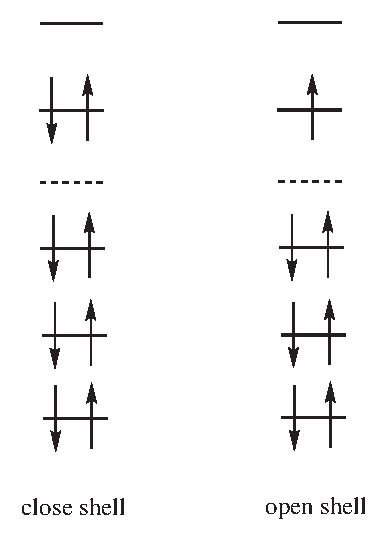
\includegraphics[scale=0.7]{rhfuhf.eps}
\caption{close shell and open shell} \label{SIC1}
\end{center}
\end{figure}

For each spatial orbital, it's only allowed maximumly $2$ electrons to reside
in. Such restriction is attributed from the Pauli principle that
there's no two electrons can share the same quantum states.
Therefore, complying with the energy minimization principle, that only
two electrons can be arranged into one orbital (such two electrons are
different in spin states).

For the quantum system which has single electron, where the number of
$\alpha$ electrons does not equal to the number of $\beta$ electrons,
the restriction above should be broken up. From the discussion of the
Hatree-Fock function, we can know that the spin is directly associated
with the total energy via the exchange effects. If the $\alpha$
electrons is more than the $\beta$ electrons, then it can be expected
that they are effected by different ``surroundings'' so that the total
energy for $\alpha$ electrons must be different with the total energy
for $\beta$ electrons. As a result, the sharing for the same spatial
orbital must be broken.

In this case, electrons in different spin states should be put into
independent spatial orbitals so that each of them forms some
independent partial orbital subspace:
\begin{equation}\label{}
\Psi =
 \begin{vmatrix}
   \varphi_{1}(1)\theta(1) &  \cdots & \varphi_{p}(1)\theta(1) & 
   \varphi_{p+1}(1)\theta(1) & \cdots  & \varphi_{n}(1)\theta(1)  \\
   \varphi_{1}(2)\theta(2) &  \cdots & \varphi_{p}(2)\theta(2) & 
   \varphi_{p+1}(2)\theta(2) & \cdots  & \varphi_{n}(2)\theta(2)  \\
   \cdots                  & \cdots  & \cdots                 & 
   \cdots                   & \cdots  & \cdots                  \\
   \varphi_{1}(n)\theta(n) & \cdots  & \varphi_{p}(n)\theta(n) & 
   \varphi_{p+1}(n)\theta(n) & \cdots  & \varphi_{n}(n)\theta(n)  \\
 \end{vmatrix}
\end{equation}
Here the $\theta(i)$ can be $\alpha(i)$ or $\beta(i)$, such method is
called unrestricted type of determinants.


%%%%%%%%%%%%%%%%%%%%%%%%%%%%%%%%%%%%%%%%%%%%%%%%%%%%%%%%%%%%%%%%%%%%%%%%%%%%%%%%%%%%%%%%%%
\section{Spin polarized states}
%
%  1  how to understand the spin polarized states
%  2  how to compose the approximated wave functions
%  3  some theorem that the alpha electrons and beta electrons
%     are forming some independent sets
%
In the above content, from the point of wave functions we have give
some general view about the spin phenomenon. In this section, we
will take another way to view the spin phenomenon in the chemistry.

In chemistry, it's very common to encounter the situation that the
characters of the given system is depending on the spin states. For
example, the characters of the radical systems etc. Here we can call
the quantum states used to describe such system as `` spin polarized
states'', which can be defined that the $\alpha$ electron density in
the given system does not equal to the $\beta$ electron density;
thus there exists some position of $\mathbf{r}$, where it has some
remaining spin:
\begin{equation}\label{}
\rho(\mathbf{r}) = \rho_{\alpha}(\mathbf{r}) -
\rho_{\beta}(\mathbf{r}) \neq 0
\end{equation}

Usually the density is expressed via the corresponding orbitals:
\begin{equation}\label{}
\rho_{\sigma}(\mathbf{r}) =
\sum_{i}|\varphi_{i\sigma}(\mathbf{r})|^{2}
\end{equation}
Where the $\sigma$ can be $\alpha$ or $\beta$. Then, the discussion
related to the spin states is attributed to the analysis on the
orbitals.

Basically there are two ways to compose the orbitals into the
approximate wave function for $n$ electrons system. One way is the
restricted method which is same as mentioned above. In this method
the $\alpha$ electrons and the $\beta$ electrons are forced into
pairs and each pair is stuffed into the orbital in the ascending
order of energy. Finally the unpaired electrons are arranged into
different orbitals. This method is also called ``restricted open
method''. The other way to compose the approximated wave function,
is the unrestricted way; that to let the $\alpha$ electrons and
$\beta$ electrons reside into different sets of orbitals, the
spatial part for the orbital for the different sets are independent
with each other.

Finally we wish to state some important distinguishment between such
two methods, is that the Slater determinant composed through the
unrestricted method is not the eigen states for the
$\hat{S}^{2}$. Hence in the post HF methods we usually do not use the
unrestricted method to compose the trial wave functions (Slater
determinant). the reason for this will be demonstrated in the next
section. 

%%%%%%%%%%%%%%%%%%%%%%%%%%%%%%%%%%%%%%%%%%%%%%%%%%%%%%%%%%%%%%%%%%%%%%%%%%%%%%%%%%%%%%%%%%
\section{General discussion for spin operators}
%
% 1  how to express the Sx, Sy, Sz
% 2  basic commutation rules on Sx, Sy, Sz
% 3  how to calculate the eigen value for the S^{2}
%    3.1  deal with Sz
%    3.2  deal with s_ and s+
%
%
for an arbitrary $n$ electrons system, we can define the spin
operator as:
\begin{equation}
  \hat{S}_{x} = \sum_{i=1}^{n}\hat{s}_{x}(i) \quad
  \hat{S}_{y} = \sum_{i=1}^{n}\hat{s}_{y}(i) \quad
  \hat{S}_{z} = \sum_{i=1}^{n}\hat{s}_{z}(i)
\end{equation}
Here each of $\hat{s}_{x}(i)$, $\hat{s}_{y}(i)$ or $\hat{s}_{z}(i)$
is working on the single particle wave function (where the ith
particle is residing in). Because we have assumed that there's no
correlation between the single particle wave functions, therefore
the total spin operator on each direction is simply the addition
between them.

Furthermore, the $\hat{S}_{x}$, $\hat{S}_{y}$ and $\hat{S}_{z}$
satisfy the basic commutation rules, which has been demonstrated in
the discussion of quantum mechanics:
\begin{align}\label{}
\hat{S}_{x}\hat{S}_{y} - \hat{S}_{y}\hat{S}_{x} &= i\hbar\hat{S}_{z}
\nonumber \\
\hat{S}_{y}\hat{S}_{z} - \hat{S}_{z}\hat{S}_{y} &= i\hbar\hat{S}_{x}
\nonumber \\
\hat{S}_{z}\hat{S}_{x} - \hat{S}_{x}\hat{S}_{z} &= i\hbar\hat{S}_{y}
\end{align}

Based on these basic spin operators, we can construct other useful
ones, namely the $\hat{S}^{2}$, $\hat{S}_{+}$ and $\hat{S}_{-}$:
\begin{equation}\label{}
\hat{S}^{2} = \hat{S}_{x}^{2} + \hat{S}_{y}^{2} + \hat{S}_{z}^{2}
\quad
\hat{S}_{+} = \hat{S}_{x} + i\hat{S}_{y} \quad
\hat{S}_{-}
=\hat{S}_{x} - i\hat{S}_{y}
\end{equation}

As what we have shown, usually in the quantum chemistry we choose
the $\hat{S}^{2}$ and $\hat{S}_{z}$ into the CSCCO, and the single
particle wave functions are always expressed as the eigen function
for the $\hat{S}_{z}$. Then for any composition based on the single
particle wave functions we can easily calculate the eigen values for
$\hat{S}_{z}$. However, how to calculate the eigen values for the
$\hat{S}^{2}$?

Here we only consider the determinants formed by the single particle
wave functions (however, it includes most of the cases in quantum
chemistry). To answer this question, we start from some relation
between the spin operators; which is easy to prove from the
definition:
\begin{equation}\label{}
\hat{S}^{2} = \hat{S}_{z}^{2} + \hat{S}_{z} + \hat{S}_{-}\hat{S}_{+}
\end{equation}

For the $\hat{S}_{z}$, to evaluate its eigen values is direct and
simple:
\begin{equation}\label{}
\left\{
  \begin{array}{ll}
    \hat{S}_{z}\alpha = \frac{1}{2} \\
    \hat{S}_{z}\beta  =-\frac{1}{2}
  \end{array}
\right.
\end{equation}
Thus for the determinant of $\Psi$, we can have:
\begin{align}\label{}
\hat{S}_{z}\Psi     &= \frac{1}{2}(n_{\alpha} - n_{\beta})\Psi
\nonumber
\\
\hat{S}_{z}^{2}\Psi &= \frac{1}{4}(n_{\alpha} - n_{\beta})^{2}\Psi
\end{align}

For the $\hat{S}_{-}$ and $\hat{S}_{+}$, it's a bit of complicated:
\begin{align}\label{}
\hat{S}_{-}\hat{S}_{+} &=
\sum_{i}\hat{s}_{-}(i)\sum_{j}\hat{s}_{+}(j)  \nonumber \\
&=\sum_{i}\hat{s}_{-}(i)\hat{s}_{+}(i) + \sum_{i \neq
j}\hat{s}_{-}(i)\hat{s}_{+}(j)
\end{align}

For the up operator and the down operator, from the basic
commutation relationship we can easily have the expressions below:
\begin{equation}\label{}
\left\{
  \begin{array}{ll}
    \hat{s}_{-}(i)\alpha(i) = \beta(i), &  \hat{s}_{-}(i)\beta(i) = 0 \\
    \hat{s}_{+}(i)\alpha(i) = 0       , &  \hat{s}_{+}(i)\beta(i) = \alpha(i) \\
  \end{array}
\right.
\end{equation}

For the determinant of $\Psi$, which can be written as:
\begin{equation}\label{}
\Psi =
\sum_{P}(-1)^{P}P(\varphi_{1}(1)\theta(1)\varphi_{2}(2)\theta(2)
\cdots\varphi_{n}(n)\theta(n))
\end{equation}

Since that the spin operator commutes with the permutation operator
of $P$, thus we can have:
\begin{multline}\label{}
\sum_{i}\hat{s}_{-}(i)\hat{s}_{+}(i)\Psi =
\sum_{P}(-1)^{P}P\Bigg\{\varphi_{1}(1)\varphi_{2}(2)
\cdots\varphi_{n}(n)
 \\
\sum_{i}\hat{s}_{-}(i)\hat{s}_{+}(i)
\Big(\theta(1)\theta(2)\cdots\theta(n)\Big)\Bigg\}
\end{multline}

In this expression, it's easy to see that only the $\beta$ electrons
can survive, thus we can have:
\begin{equation}\label{}
\sum_{i}\hat{s}_{-}(i)\hat{s}_{+}(i)\Psi = n_{\beta}\Psi
\end{equation}

On the other hand,  for the given $i$ and $j$; we have:
\begin{equation}\label{}
\begin{split}
\hat{s}_{-}(i)\hat{s}_{+}(j)\Psi &=
\sum_{P}(-1)^{P}P\Bigg\{\varphi_{1}(1)\varphi_{2}(2)
\cdots\varphi_{n}(n)
 \\
&\hat{s}_{-}(i)\hat{s}_{+}(j)
\Big(\theta(1)\cdots\alpha(i)\beta(j)\cdots\theta(n)\Big)\Bigg\} \\
    &=
\sum_{P}(-1)^{P}P\Bigg\{\varphi_{1}(1)\varphi_{2}(2)
\cdots\varphi_{n}(n)
 \\
&\Big(\theta(1)\cdots\beta(i)\alpha(j)\cdots\theta(n)\Big)\Bigg\} \\
\end{split}
\end{equation}

Therefore, the $\sum_{i \neq j}\hat{s}_{-}(i)\hat{s}_{+}(j)$ change
all the pairs of $\alpha(i)\beta(j)$ to be $\beta(i)\alpha(j)$, then
form new determinants. So we can abbreviate this operator as
$\sum_{i \neq j}\hat{P}_{ij}$.

All in all, we can have:
\begin{align}\label{SICeq:3}
\hat{S}^{2}\Psi &= \left(\frac{1}{4}(n_{\alpha} - n_{\beta})^{2} +
\frac{1}{2}(n_{\alpha} - n_{\beta}) + n_{\beta} + \sum_{i \neq
j}\hat{P}_{ij}\right)\Psi \nonumber \\
&=\left(\frac{1}{4}(n_{\alpha} - n_{\beta})^{2} +
\frac{1}{2}(n_{\alpha} + n_{\beta})\right)\Psi + \sum_{i \neq
j}\hat{P}_{ij}\Psi
\end{align}

Now take the $\Psi = |1s(1)\alpha(1)1s(2)\beta(2)2s(3)\alpha(3)|$ as
an example, to see that how to use the (\ref{SICeq:3}) to calculate
the eigen value for the $\hat{S}^{2}$:
\begin{equation}\label{}
\begin{split}
\hat{S}^{2}\Psi &= \left(\frac{1}{4}(2 - 1)^{2} + \frac{1}{2}(2 +
1)\right)|1s(1)\alpha(1)1s(2)\beta(2)2s(3)\alpha(3)| + \\
&|1s(1)\beta(1)1s(2)\alpha(2)2s(3)\alpha(3)| +
|1s(1)\alpha(1)1s(2)\alpha(2)2s(3)\beta(3)| \\
&=\frac{7}{4}|1s(1)\alpha(1)1s(2)\beta(2)2s(3)\alpha(3)| -
|1s(1)\alpha(1)1s(2)\beta(2)2s(3)\alpha(3)| \\
&=\left(\frac{1}{2}(\frac{1}{2} +
1)\right)|1s(1)\alpha(1)1s(2)\beta(2)2s(3)\alpha(3)|
\end{split}
\end{equation}
Thus, it's the eigen function for $\hat{S}^{2}$, and give the eigen
value of $3/4$.

Now finally let's give some illustration about some important concept
that why the unrestricted determinant is not the eigen function for
$\hat{S}^{2}$; this can be made clear through the definition of
$\hat{S}^{2}$ in (\ref{SICeq:3}). 

Take $|1s(1)\alpha(1)1s^{'}(2)\beta(2)|$ as an example. This
determinant gives $S_{z} = 0$, and it can be used to portray the
ground state for hydrogen gas ($H_{2}$). By the definition of
$\hat{S}^{2}$ in (\ref{SICeq:3}), we can have:
\begin{equation}
  \begin{split}
    \hat{S}^{2} |1s(1)\alpha(1)1s^{'}(2)\beta(2)| &= \left( 0 +
      1\right)|1s(1)\alpha(1)1s^{'}(2)\beta(2)| + \\
    & |1s(1)\beta(1)1s^{'}(2)\alpha(2)| \\
&=  |1s(1)\alpha(1)1s^{'}(2)\beta(2)| +
    |1s(1)\beta(1)1s^{'}(2)\alpha(2)|
  \end{split}
\end{equation}
Compared with the former example for
$|1s(1)\alpha(1)1s(2)\beta(2)2s(3)\alpha(3)|$, here the
distinction is that in the second determinant of
$|1s(1)\beta(1)1s^{'}(2)\alpha(2)|$; if we exchange the electron label
between $1$ and $2$, we will get $|1s^{'}(1)\alpha(1)1s(2)\beta(2)|$,
which is obviously different from the first one. Hence the inequality
of the partial part of MO lead to the determinants unable to cancel
with each other. That's why the unrestricted type of determinants are
no longer to be the eigen states for the $\hat{S}^{2}$. 



%%%%%%%%%%%%%%%%%%%%%%%%%%%%%%%%%%%%%%%%%%%%%%%%%%%%%%%%%%%%%%%%%%%%%%%%%%%%%%%%%%%%%%%%%%
\section{How to form the spin adapted configurations}
%
%
%  in this part, we discuss that how to form the
%  spin adapted configurations
%  1   general strategy
%  2   discuss the singlet, doublet and triplet.
%      the eigen states and eigen values
%  3   extend the idea to arbitrary sin states
%
%
Now based on the discussion above, let's talk about that how to form
the spin adapted configurations; which is one of important step in
CI and it's derivative methods.

Basically, the spin adapted configurations in the trial wave
functions can be achieved by the following two steps:
\begin{itemize}
  \item Selecting orbitals to form the Slater determinants.
  From the result of Hatree-Fock calculation, we can select
  a group of orbitals to form the determinants. Here the
  Slater determinants should be only formed in restricted way
  because only this kind of determinants can be the eigen states for
  the $\hat{S}^{2}$ and $\hat{S}_{z}$.
\item After the first step, the determinants will be combined into
  some linear combination so that it's the eigen states for the
  $\hat{S}^{2}$ and $\hat{S}_{z}$. Here we may apply some techniques to
  do so, for example to use the project operator to ``sort out'' the
  Slater determinants we want. Finally, we can get the so called
  ``spin adapted configurations''. According to the rules introduced
  above, the spin adapted configurations which give different eigen
  values for the $\hat{S}^{2}$ or $\hat{S}_{z}$ will not mixing with
  each other, so the Hamiltonian matrix will be shaped into blocks.
\end{itemize}

Next, we wish to present several examples to show how to construct
the spin adapted configurations. In the discussion below the general
form of determinants will be considered ($n$ electrons are arranged
into $m$ orbitals):
\begin{equation}\label{}
\Psi = |\varphi_{1}(1)\theta(1)\cdots\varphi_{m}(n)\theta(n)|
\end{equation}

the most simplest eigen state for the spin operator of $\hat{S}^{2}$
and $\hat{S}_{z}$ is the singlet, which can be defined as:
\begin{equation}\label{SICeq:4}
\left\{
  \begin{array}{ll}
    \hat{S}_{z}\Psi = 0 \Rightarrow S = \max(S_{z}) = 0\\
    \hat{S}^{2}\Psi = S(S+1) = 0
  \end{array}
\right.
\end{equation}
Here, for a certain $S$ there will be $2\max(S_{z}) + 1$ degenerate
states, they are different in $S_{z}$; thus we can see that there's
only one eigen state satisfy the (\ref{SICeq:4}); so we call this
state as ``singlet''.

It's easy to see that only the close shell determinant can be the
singlet (see the figure of \ref{SIC2}). In the open shell case, we
can reverse the spin on Z direction for the unpaired electrons so
that to form the determinants which have different $S_{z}$ value.
but they can also correspond to same $\hat{S}$. Therefore, there are
more than one determinants corresponding to the $\hat{S}$ so that the
open shell determinants can not correspond to the singlet.
\begin{figure}
\begin{center}
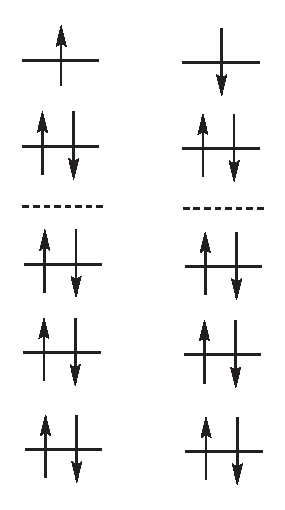
\includegraphics[scale=0.7]{spin_chem_1.eps}
\caption{doublet states} \label{SIC2}
\end{center}
\end{figure}

Similarly we can define the ``doublet'' states, which is:
\begin{equation}\label{SICeq:5}
\left\{
  \begin{array}{ll}
    \hat{S}_{z}\Psi = \frac{1}{2}, -\frac{1}{2}
    \Rightarrow S = \max(S_{z}) = \frac{1}{2}\\
    \hat{S}^{2}\Psi = S(S+1) = \frac{3}{4}
  \end{array}
\right.
\end{equation}
It's called doublet because for a certain $S$ it has two degenerate
states, one gives the eigen value of $1/2$ for $\hat{S}_{z}$, the
other gives $-1/2$. Such determinants are pictured in (\ref{SIC2}).

Moreover, we can see that the doublet can only be the determinants
shown in figure of (\ref{SIC2}). If there are more than two orbitals
having the single electron residing on, we can see that the maximum
of $S_{z}$ must exceed or equal to $1$ ($\max(S_{z}) \leq 2*1/2 =
1$), thus there will be at least $3$ eigen states for the
$\hat{S}_{z}$, so it's not the doublet.

On the other hand, we can use the $\hat{S}^{2}$ defined in
(\ref{SICeq:3}) to prove that each of the determinant is the eigen
state for $\hat{S}^{2}$. For the doublet, we can generally assume
the single electron residing on its highest orbital:
\begin{align}\label{SICeq:6}
\Psi &= |\varphi_{1}(1)\alpha(1)\varphi_{1}(2)\beta(2) \cdots
\nonumber \\
&\varphi_{m-1}(n-1)\alpha(n-1)\varphi_{m-1}(n-1)\beta(n-1)
\varphi_{m}(n)\theta(n)|
\end{align}
Here the $\theta(n)$ can be $\alpha$ or $\beta$.

In the expression of the $\hat{S}^{2}$, we can see that operator of
$\sum_{i \neq j}\hat{P}_{ij}$ should only change the pair of
electrons which share the same orbitals, else there will be pair of
electrons with same spin states on the same orbital, it will be
zero. So we can have (here below the total number of electrons are
$2n+1$):
\begin{equation}\label{}
\begin{split}
\hat{S}^{2}\Psi &= \left(\frac{1}{4} + \frac{1}{2}(2n +
1)\right)\Psi + n|\varphi_{1}(1)\alpha(1)\varphi_{1}(2)\beta(2)
\cdots  \\
&\varphi_{i}(k)\beta(k)\varphi_{i}(k+1)\alpha(k+1)\cdots
\varphi_{m}(n)\theta(n)| \\
&=\frac{3}{4}\Psi + n\Psi -n\Psi \\
&=\left(\frac{1}{2}(\frac{1}{2} + 1)\right)\Psi
\end{split}
\end{equation}

Next, we can discuss the ``triplet'', which is defined as:
\begin{equation}\label{SICeq:7}
\left\{
  \begin{array}{ll}
    \hat{S}_{z}\Psi = 1, 0,  -1
    \Rightarrow S = \max(S_{z}) = 1\\
    \hat{S}^{2}\Psi = S(S+1) = 2
  \end{array}
\right.
\end{equation}
Thus for the $S=1$ there are three eigen states corresponding to
different $S_{z}$ values. Similar with the discussion for singlet
and doublet, we can see that the triplet state should has two single
electron orbitals, which can be pictured in the figure of
(\ref{SIC3}).
\begin{figure}
\begin{center}
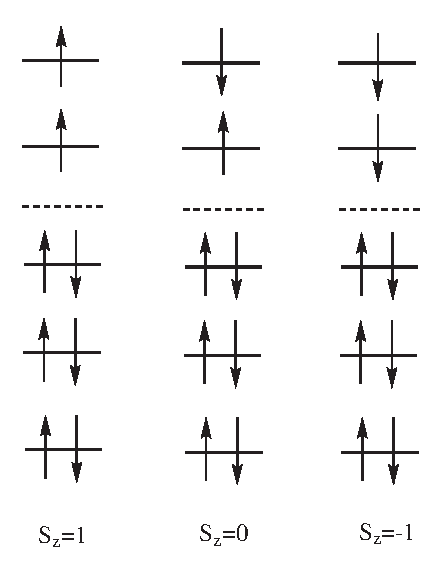
\includegraphics[scale=0.7]{triplet.eps}
\caption{how to form a triplet} \label{SIC3}
\end{center}
\end{figure}

Now we derive the expression of the triplet eigen states for both of
the $\hat{S}^{2}$ and $\hat{S}_{z}$. It's assumed that the
determinants has such form:
\begin{equation}\label{}
\Psi = |\varphi_{1}(1)\alpha(1)\varphi_{1}(2)\beta(2) \cdots
\varphi_{m-1}(n-1)\theta(n-1) \varphi_{m}(n)\theta^{'}(n)|
\end{equation}
Here the $\theta$ and $\theta^{'}$ can be $\alpha$ or $\beta$.

Firstly we note that this case is different form the singlet and
doublet, where all the eigen states for the $\hat{S}^{2}$ and
$\hat{S}_{z}$ are non-degenerate; here the $\hat{S}_{z}$ has two
degenerate eigen states, they all give $S_{z} = 0$:
\begin{equation}\label{}
\Psi_{01} = |\varphi_{1}(1)\alpha(1)\varphi_{1}(2)\beta(2) \cdots
\varphi_{m-1}(n-1)\alpha(n-1) \varphi_{m}(n)\beta(n)|
\end{equation}
\begin{equation}\label{}
\Psi_{02} = |\varphi_{1}(1)\alpha(1)\varphi_{1}(2)\beta(2) \cdots
\varphi_{m-1}(n-1)\beta(n-1) \varphi_{m}(n)\alpha(n)|
\end{equation}
Therefore, for the $S_{z} = 0$, the eigen state of the $\hat{S}^{2}$
must be the linear combination between the two determinants. By
using the $\hat{S}^{2}$ defined in (\ref{SICeq:3}), we can finally
have:
\begin{equation}\label{}
\Psi_{0} = \frac{1}{\sqrt{2}}(\Psi_{01} + \Psi_{02})
\end{equation}

On the other hand, for the $S_{z} = 1$ and $S_{z} = -1$, the eigen
states are non-degenerate:
\begin{equation}\label{}
\Psi_{1} = |\varphi_{1}(1)\alpha(1)\varphi_{1}(2)\beta(2) \cdots
\varphi_{m-1}(n-1)\alpha(n-1) \varphi_{m}(n)\alpha(n)|
\end{equation}
\begin{equation}\label{}
\Psi_{-1} = |\varphi_{1}(1)\alpha(1)\varphi_{1}(2)\beta(2) \cdots
\varphi_{m-1}(n-1)\beta(n-1) \varphi_{m}(n)\beta(n)|
\end{equation}
Thus they must be the eigen states for the $\hat{S}^{2}$. By using
the expression in (\ref{SICeq:3}), we can also prove this point.

From the three examples above we can extend the idea to the
arbitrary spin states. For some spin state of $\Psi$ where the
spatial orbitals are fixed, we can construct a lot of eigen states
for $\hat{S}_{z}$, and some may be degenerate. For these degenerate
states the eigen state for the $\hat{S}^{2}$ must be linear
combination of them. For deriving the eigen states for both of the
$\hat{S}_{z}$ and $\hat{S}^{2}$, it has been developed many
effective methods such as the ``Young Picture''
method\cite{aoqingTang}. The reader can refer to such materials for
more help.


%%%%%%%%%%%%%%%%%%%%%%%%%%%%%%%%%%%%%%%%%%%%%%%%%%%%%%%%%%%%%%%%%%%%%%%%%%%%%%%%%%%%%%%%%%
\section{Spin contamination}
%
% 1  give the general expression for the unrestricted wave function
% 2  why the states are mixed together
% 3  the reason for the spin contamination
% 4  how to reduce the spin contamination
%
The unrestricted type of wave functions usually have the spin
contamination problem. This problem is attributed from the mixture
of other spin states.

For the general unrestricted wave function of $\Psi$, the general
expression is below (we suggest that we have $k$ $\alpha$ electrons
and $l=n-k$ $\beta$ electrons):
\begin{equation}\label{}
\Psi =
 \begin{vmatrix}
   \varphi_{1}(1)\theta(1) &  \cdots & \varphi_{p}(1)\theta(1) & 
   \varphi_{p+1}(1)\theta(1) & \cdots  & \varphi_{n}(1)\theta(1)  \\
   \varphi_{1}(2)\theta(2) &  \cdots & \varphi_{p}(2)\theta(2) & 
   \varphi_{p+1}(2)\theta(2) & \cdots  & \varphi_{n}(2)\theta(2)  \\
   \cdots                  & \cdots  & \cdots                 & 
   \cdots                   & \cdots  & \cdots                  \\
   \varphi_{1}(n)\theta(n) & \cdots  & \varphi_{p}(n)\theta(n) & 
   \varphi_{p+1}(n)\theta(n) & \cdots  & \varphi_{n}(n)\theta(n)  \\
 \end{vmatrix}
\end{equation}

Commonly we do not require that the spatial part of orbital for
$\alpha$ electron and $\beta$ electron should be same, because
they varies independently. In such circumstance, the wave function
is the eigen state for the $\hat{S}_{z}$, because it gives certain
eigen value for the $\hat{S}_{z}$ ($S_{z} = \frac{1}{2}(k-l)$).
However, such wave function is usually not the eigen function for
the $\hat{S}^{2}$, which is just as what we have demonstrated.

From the spin discussion in quantum mechanics, we know that for the
eigen states with some certain $S_{z}$ (e.g. $S_{z} = 1$); there may
exist many states corresponding to it, they come from the eigen
states with different $S$ eigen value (for example, as $S_{z} = 1$,
it has eigen states coming from $S=1,2,3 \cdots$).

According to such analysis, we can have the general principle below;
that the unrestricted wave function of $\Psi$ with $S_{z} = m$, can
be composed by the eigen states whose $S_{z} = m$, but their $S =
m+2, m+4, m+6, \cdots$ etc.:
\begin{align}\label{}
\Psi_{siglet} &= c_{1}\ket{1} + c_{2}\ket{3} + c_{3}\ket{5} + \cdots
\nonumber \\
\Psi_{doublet} &= c_{1}\ket{2} + c_{2}\ket{4} + c_{3}\ket{6} +
\cdots
\nonumber \\
\Psi_{triplet} &= c_{1}\ket{3} + c_{2}\ket{5} + c_{3}\ket{7} +
\cdots
\end{align}

Here we have some question that for the $\Psi$ with $S_{z} = m$, why
the $m+1$, $m+3$ states etc. do not contribute to it?

To answer this question, we have to remember that for the state with a
certain $S$ value, it only has one eigen state that $S_{z} = m$.  If
the spatial part of the determinants are fixed, and we require that it
gives certain $S$ value; since $S = \max (S_{z})$, and the number of
single electrons in the determinant is $2\max (S_{z})$; hence the
number of single electrons are $2S$. 

In this case, the higher spin state with different $S$ value should be
those that ``fire up'' the electrons from the occupied orbitals to the
virtual orbitals so as to produce new single electrons in this
determinant. In this process, the action will always generate two new
single electron orbital, thus the higher spin states should increase
by degrees by $2$ (obviously this value is related to the $S$
according to the analysis above).

Based on the analysis above, we can know that the spin contamination
is some inherent character for the unrestricted wave functions.
Traditionally in quantum chemistry, there has been developed many
ways to reduce the spin contamination, such as the use of
``annihilate operator'' to project the right component of the spin
state from the mixtures. For further study, the reader may also
refer to the book given by Tang\cite{aoqingTang}.

%%%%%%%%%%%%%%%%%%%%%%%%%%%%%%%%%%%%%%%%%%%%%%%%%%%%%%%%%%%%%%%%%%%%%%%%%%%%%%%%%%%%%%%%%%


%%% Local Variables: 
%%% mode: latex
%%% TeX-master: "../../main"
%%% End: 

%%
% revised in Jan, 18th, 2008
% problems left behind:
% 1   whether we can have such extension:
% \begin{equation}\label{GROUPeq:8}
%     \hat{O}_{R}[\Psi\Phi] = (\hat{O}_{R}\Psi)(\hat{O}_{R}\Phi)
%     \end{equation}
%     I am not sure that whether it's correct.  2 vanishing integrals
%     is not fully finished, something is still missing; perhaps
%     better to rewrite some of the content
%
%
%

%%%%%%%%%%%%%%%%%%%%%%%%%%%%%%%%%%%%%%%%%%%%%
\chapter{Group Theory in Quantum Chemistry}
%
% introduction: what's the group theory origin.
%
%
Group theory is a branch of pure mathematics, but it plays an
important role in quantum mechanics. Qualitative information about
molecular wave function and its property can always be obtained from
the symmetry of molecule. In essence, the symmetry of molecule is one
of its fundamental property, which is originated from the uncertainty
principle of the quantum particles.

Before stepping in the detailed discussion, it's very interesting to
take a general view about the comparison between classic mechanics and
quantum mechanics. In the macroscopic world, there never has two
objects that are exactly same with each other; but in the quantum
world, because of the uncertainty principle, if the particles belongs
to the same type, for example, two electrons, and two hydrogen atoms;
it's impossible to distinguish them between each other. So two
electrons actually are the same, and so as the atoms.  Thus the
symmetry of the molecule is a result of the uncertainty principle. In
a sense, the symmetry is some kind of inherent and fundamental
property embedded in the molecule. The description here in this
chapter is basically taken from two books given by Bishop\cite{Bishop}
and Cotton\cite{Cotton}.

%%%%%%%%%%%%%%%%%%%%%%%%%%%%%%%%%%%%%%%%%%%%
\section{The concept of symmetry operation}\label{GROUP13}
% 1 definition of the symmetry operation and symmetry element as well
% as their difference 2 how to understand the symmetry operation
%
%
Before we started, it's necessary for us to distinguish an important
concept: that the difference between symmetry operation and symmetry
element. Symmetry operation is the transformation of a body such that
the final position is physically indistinguishable from the initial
position. Symmetry elements is the geometrical entity (point, line or
plane) with respect to which a symmetry operation is carried out. So
we can see that they are conceptually different.  Furthermore, the
point group we will discuss here, is related to the group of symmetry
operations; and the symmetry element is a way to help us to
intuitively understand the symmetry operation.

The introduction of the concept of symmetry operation is vital to the
use of group theory in the chemistry. This concept generalizes the
intrinsic symmetric property of the molecules, through this concept
the application of the group theory is made possible.  Therefore, the
symmetry operation is the most fundamental concept in this subject.

How can we understand the symmetry operations? To some extent, the
symmetry operation is similar to the operator in the quantum
mechanics. Symmetry operation is only some general and abstract form
of operation, as we use different ``bases'' on which the symmetry
operation is applied, there will be accordingly different ways to
represent the same symmetry operation. For example, if we use the
coordinates of an atom (the base is the coordinates), then the
symmetry operation will naturally correspond to some $3\times 3$
matrix which converts one position of atom to another. If we use the
coordinates from s specific molecule (for example, a molecule contains
$9$ atoms), then the same symmetry operation will be some $27\times
27$ matrix working on the coordinates of the bunch of atoms. On the
other hand, if the atom orbitals(or more specifically to say, the
basis functions) are used, the symmetry operation will be the matrix
that describing the mixture of the corresponding orbitals. However, no
matter what kind of representations the symmetry operation is chosen
to be, they all reflect the same essence behind it; that's why we can
use the abstract group theory to describe such generalized concept.

%%%%%%%%%%%%%%%%%%%%%%%%%%%%%%%%%%%%%%%%%

\subsection{Fundamental symmetry operations}
%
% 1 five fundamental symmetry operations 2 why the Sn is fundamental?
% 3 further discussion to the Sn
%

There are five fundamental symmetry operations; in a sense that all
the other symmetry operations can be composed from them.
\begin{itemize}
\item rotation over an axis ($C_{n}$)
\item inversion related to a point ( i )
\item reflection through a mirror of plane ($\sigma$)
\item rotation over an axis then plus reflection through a mirror of
  plane (here the index of h means that the plane is vertical to the
  axis) ($S_{n} = \sigma_{h} C_{n}$)
\item identical operation ($E$)
\end{itemize}

It's very natural to understand the symmetry operation of reflection,
inversion and rotation. Such operations are represented by the
fundamental symmetry elements of point, axis and plane.  Identical
operation of $E$ makes the molecule unchanged, actually it's the
identity element in the point group. Any group can not be short of the
identity element, so it's a fundamental operation.

Here is an interesting question that why the rotation-reflection
$S_{n}$ is a fundamental operation? Actually we can find that there
has some molecule that only has the $S_{n}$ operation, where the
rotation operation and reflection operation are absent. Therefore,
$S_{n}$ is symmetry operation independent of $C_{n}$ and
$\sigma_{h}$. Here below the (\ref{GROUP11}) shows that how to make a
$S_{n}$ symmetry operation.

\begin{figure}[htp]
  \begin{center}
    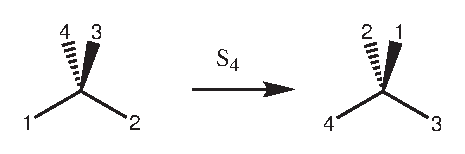
\includegraphics[scale=0.7]{s4.eps}
    \caption{an example that how to make S4 symmetry operation}
    \label{GROUP11}
  \end{center}
\end{figure}

To further understand this situation, there are several general rules
respect to the connection between $S_{n}$ and $C_{n}, \sigma$.
\begin{itemize}
\item if $n$ is odd number, the $S_{n}$ is the direct product of
  $C_{n}$ and $\sigma_{h}$; here the $S_{n}$ is the combination
  between the $C_{n}$ and $\sigma$. the case of $S_{3}$ clearly
  demonstrates such rules.
\item if $n$ is an even number, the case should be divided into two
  subgroups:
  \begin{itemize}
  \item if the $n=4k$, $S_{n}$ is an unique and independent symmetry
    operation, together with the $C_{\frac{n}{2}}$ symmetry operation.
  \item for the other cases, the $S_{n}$ is composed by the
    $C_{\frac{n}{2}}$ and $\sigma_{h}$. The case of $S_{6}$ will show
    this.
  \end{itemize}
\end{itemize}

the $S_{4}$ is:
\begin{eqnarray}\label{GROUPeq:2}
  S^{1}_{4} &=& \sigma_{h}C^{1}_{4}  \nonumber \\
  S^{2}_{4} &=& \sigma^{2}_{h}C^{2}_{4} = C^{1}_{2} \nonumber \\
  S^{3}_{4} &=& \sigma_{h}C^{3}_{4}   \nonumber \\
  S^{4}_{4} &=& E  \nonumber \\
  S^{i}_{4} &=& S^{i-4}_{4} (i > 4)
\end{eqnarray}

the $S_{3}$ is:
\begin{eqnarray}\label{GROUPeq:3}
  S^{1}_{3} &=& \sigma_{h}C^{1}_{3}                 \nonumber \\
  S^{2}_{3} &=& \sigma^{2}_{h}C^{2}_{3} = C^{2}_{3} \nonumber \\
  S^{3}_{3} &=& \sigma_{h}C^{3}_{3} = \sigma_{h}    \nonumber \\
  S^{4}_{3} &=& C^{1}_{3}                           \nonumber \\
  S^{5}_{3} &=& \sigma_{h}C^{2}_{3}                 \nonumber \\
  S^{6}_{3} &=& E
\end{eqnarray}
Here we can see that the $S_{3}$ reproduce the group of $C_{3}\otimes
\sigma_{h}$.


Now let's see the case of $S_{6}$.

\begin{eqnarray}\label{GROUPeq:4}
  S^{1}_{6} &=& \sigma_{h}C^{1}_{6}                 \nonumber \\
  S^{2}_{6} &=& \sigma^{2}_{h}C^{1}_{3} = C^{1}_{3} \nonumber \\
  S^{3}_{6} &=& \sigma_{h}C^{1}_{2} = i             \nonumber \\
  S^{4}_{6} &=& C^{2}_{3}                           \nonumber \\
  S^{5}_{6} &=& \sigma_{h}C^{5}_{6}                 \nonumber \\
  S^{6}_{6} &=& E
\end{eqnarray}

Hence, we can see that $S_{4k}$ is indecent of the $C_{n}$ and
$\sigma$, as in $S_{4}$ there's no $\sigma$ operation.

%%%%%%%%%%%%%%%%%%%%%%%%%%%%%%%%%%%%%%
\subsection{Algorithm between symmetry operation}
%
% 1 multiplication 2 commutative character 3 division 4 do not have
% addition ??
%
%
After setting up the fundamental symmetry operation, now in this
section we are going to demonstrate the algorithm between them.

The symmetry operations can be multiplied like operators. If $P$ and
$Q$ are two symmetry operations, their product of $PQ$ is naturally
the symmetry operation, too. Such multiplication is defined by the way
that first to apply the symmetry operation $Q$, then apply the
symmetry operation $P$:
\begin{equation}\label{}
  R = PQ
\end{equation}
Similar to the operator that the multiplication order is important.
Generally we have that $PQ \neq QP$. For example, for the $NH_{3}$
molecule it has $C_{3}$ and $\sigma$ operations, but we can see that
(this molecule has three reflection mirrors, they are labeled by $1$,
$2$ and $3$; separately):
\begin{equation}\label{}
  C_{3}^{1}\sigma_{1} = \sigma_{2} \quad  \sigma_{1}C_{3}^{1} =
  \sigma_{3}
\end{equation}
Therefore different order produce different results. However, there
exists some symmetry operations which do not care about the order:
$PQ=QP$, it's said that they are commutative. For example, $C_{3}$ and
$i$ are two commutative operations.

The multiplication between symmetry operations satisfy the commutation
rules below:
\begin{equation}\label{}
  (PQ)R = P(QR) = PQR
\end{equation}

The division algorithm, which is considered to be the counter
algorithm of the multiplication; can be defined that:
\begin{equation}\label{}
  PQ = E \Rightarrow P = Q^{-1}
\end{equation}
Since that any symmetry operation all has its counter operation (this
is the requirement by the group theory), thus for any point group, the
identity operation of $E$ always exists.

The algorithms concerned with the symmetry operation are mainly
related to the multiplication and division. It's interesting that
there's no addition, substraction etc. for the symmetry operations,
although in the quantum mechanics the operator has such operations.
That's because the addition etc. have no physical correspondence to
the symmetry operation, we do not know how to define the physical
process for the addition of two symmetry operations.

%%%%%%%%%%%%%%%%%%%%%%%%%%%%%%%%%%%%%%%%%%
\subsection{Product rules between symmetry operations}
%
% 1 we can form any groups based on the fundamental five symmetry
% operations 2 rules related to the product between symmetry
% operations 3 commutative rules between symmetry operations
%
So far, we have five fundamental symmetry operations, each of them can
form an independent group, and is labeled with an unique symmetry
element. They are:
\begin{itemize}
\item rotation group $C_{n}$: $\{E, C^{1}_{n}, C^{2}_{n}, \cdots,
  C^{n-1}_{n}\}$
\item reflection group $\sigma$: $\{E, \sigma \}$
\item inversion group $i$: $\{E, i \}$
\item rotation-reflection group $S_{n}$: $\{E, S^{1}_{n}, S^{2}_{n},
  \cdots, S^{n-1}_{n} \}$
\item identical group $E$: $\{E \}$
\end{itemize}

To some extent, the point group can be seen as the combination of such
five fundamental groups. Here between them, the presence of some
special symmetry elements will lead to the existence of some other
symmetry elements. In the content below, we are going to state such
summarized rules.
\begin{itemize}
\item combination of two rotation axes
  \begin{itemize}
  \item If two $C_{2}$ axes crosses with each other with an angle of
    $\frac{2\pi}{2n}$, there has a $C_{n}$ axis drilling through the
    cross point and perpendicular with the plane forming by the two
    $C_{2}$ axes. \\
    On the other hand, if there exists a $C_{n}$ axis and a $C_{2}$
    axis which is vertical to the $C_{n}$ axis; another $C_{2}$ axis
    which satisfies the above condition also holds its presence.
  \end{itemize}
\item combination of two mirrors
  \begin{itemize}
  \item If two mirrors crosses with each other with an angle of
    $\frac{2\pi}{2n}$, the cross line is a $C_{n}$ axis. On the other
    hand, if we have a $C_{n}$ axis and a reflection mirror through
    it, the rotation of the mirror leads to $n$ mirrors; with an angle
    of $\frac{2\pi}{2n}$ between any adjacent mirror pairs .
  \end{itemize}
\item combination between axis and mirror
  \begin{itemize}
  \item If we have an even $C_{n}$ axis with a mirror vertical to it,
    the cross point must be inversion point. Similarly if we have an
    inversion point and a mirror through it, we have a $C_{2}$ axis
    perpendicular to the mirror and through the inversion point.
  \end{itemize}
\end{itemize}

For the commutative character of the symmetry operation, it can be
proved that the pairs of symmetry operations below are always
commutative.
\begin{itemize}
\item two rotations around same axis
\item reflection through two perpendicular mirror
\item inversion and any rotation or reflection
\item rotations in succession on two vertical $C_{2}$ axis
\item rotation and reflection where the mirror vertical to the
  rotation axis
\end{itemize}


%%%%%%%%%%%%%%%%%%%%%%%%%%%%%%%%%%%%%
\section{Point group}
% 1 the definition of the point group, it's the unit for study 2 why
% called point group
%
What is the point group? The point group is the collection of all the
symmetry operations corresponding to some specifical molecules.
Mathematically, such collection forms an entire and complete group,
each possesses some individual characters. Here it's noted that the
point group is the unit for studying the application of group theory
on the chemistry.

The point group can always judged from the outside appearance of the
molecules. For example, the carbon dioxide molecule and the hydrogen
gas molecule are belonging to the same kind, because they own the same
kind of symmetry operations. On the other hand, the water molecule has
the different point group with the molecules mentioned above.

For a given molecule, since that the translation can not alter its
symmetry properties, all the symmetry operations should be all through
one point (this point is not varied for any symmetry operations. For a
single molecule, this point is its center of mass). Therefore the
point group is also called molecule group.


%%%%%%%%%%%%%%%%%%%%%%%%%%%%%%%%%%%%%%%%
\subsection{Conjugation in symmetry operations}
%
% 1 mathematically define the conjugation 2 three characters related
% to the conjugation 3 class definition, and it's not subgroup 4
% connection between commutation and conjugation
%
%
In a given point group of $G$, and if we have element of $C$ to make
operation $A$ and $B$ satisfy that $AC=CB$ (this is equivalent to
$C^{-1}AC = B$ since $C^{-1}$ always exists); then $A$ and $B$ are
called conjugated with each other.

We can prove the following characters related to the conjugation.
First, $A$ always conjugated to itself, that is we can always find
some $X$, to make $A = X^{-1}AX$.
\begin{equation}\label{}
  A^{-1}A = A^{-1}X^{-1}AX = (AX)^{-1}AX = E
\end{equation}
Here, we can always has $X = E$, but we may also find some others to
get the equation. For example, we have $i^{-1}C^{1}_{3}i = C^{1}_{3}$;
this is because $i$ and $C^{1}_{3}$ are commutative.

Second, $A$ conjugates with $B$ is equivalent to that $B$ conjugates
with $A$.
\begin{equation}\label{}
  X^{-1}AX = B \Leftrightarrow A = XBX^{-1}
\end{equation}

Third, if $A$ and $B$ are conjugated, and $B$ and $C$ are conjugated;
then $A$ and $C$ are conjugated, too.
\begin{align}\label{}
  P^{-1}AP = B  & \quad  Q^{-1}BQ = C \Rightarrow \nonumber \\
  Q^{-1}P^{-1}APQ &= R^{-1}AR = C
\end{align}
Here, $R = PQ$. Thus, the conjugated character can be passed from one
to another.

It's interesting to see that from the above three characters, it
implies that the operation of conjugation seems to be
``self-contained''. In fact, the elements which conjugated with each
other in a given group forms a ``class''; such class is some kind of
self-contained.

However, here the meaning of self-contained does not denote that the
class is forming a subgroup. For example, the symmetry operations for
the $NH_{3}$ molecule has been classified into three classes: $E$,
$\sigma_{1}, \sigma_{2},\sigma_{3}$ and $C^{1}_{3}, C^{2}_{3}$.  We
can see that in the second and third class there has not $E$ so that
they can not be subgroups.

On the other hand, there's no direct relations between commutation and
the conjugation. For example, the symmetry operations of $C^{i}_{n}
(i=1,2,\cdots,n)$ are commutative, but they are not in one class(from
the definition we can see this point. For any $C^{i}_{n} = P$ and
$C^{j}_{n} = Q$, and $i \neq j$; we always have $Q^{-1}PQ \equiv P$
for any $Q$). Generally, if the point group is an Abel kind, the
different elements in this group are in separate class, the number is
same to the order of the group.

%%%%%%%%%%%%%%%%%%%%%%%%%%%%%%%%%%%%%%%%
\subsection{Equivalent symmetry operations}
%
% this section talk about the conjugation in intuitional way
%
%
%
In the $C^{-}AC=B$, the $A$ and $B$ are called equivalent symmetry
operations. In this section, we are going to provide some way to
understand them in some intuitional way.

Firstly, we note that symmetry operation to the molecular coordinates
while retaining the coordinate system unchanged is identical to the
way that operation to the coordinate system while keeping the molecule
coordinates unchanged. This fact is easily understood in three
dimensional space. Therefore it turns out that we can interpret the
$C^{-}AC=B$ in this way:
\begin{quote}
  \begin{center}
    first the $C$ operation is made to the coordinate system to
    transform it to the new one, then in the new coordinate system the
    $A$ operation is made to the molecule coordinates; then finally
    the $C^{-}$ operation makes the new coordinates system restores to
    original one. From the equality, this process will generate the
    $B$ operation.
  \end{center}
\end{quote}

This is some very interesting interpretation. Here, it also implies
that why we call them as ``equivalent'' symmetry operations. Through
this process, we can clearly see that $A$ and $B$ are equivalent as
long as that they are the same symmetry operation by executing in
different coordinate system (here in the above interpretation, the $A$
happens in the new one changed by the $C$, and the $B$ happens in the
old one; but they lead to the same result).

On the other hand, by the similar way we can understand the equivalent
symmetry operation in another way; that if there exists a symmetry
operation working on the coordinate system, which is able to replace
$A$ by $B$ ($A$ and $B$ are also the symmetry operation in this
group); then $A$ and $B$ are conjugated with each other (they are also
the equivalent symmetry operations).

The understanding of this issue is same with the way above. Since that
we have $AC=CB$ for conjugated $A$ and $B$, if we can find the $C$
working on the coordinate system (that is equivalent to working on the
molecule itself); then the $AC$ means to change the coordinate system
by $C$, then apply the $A$ to the molecule. That is same to apply the
$B$ to the molecule, then change the coordinate system by $C$. Thus,
if $A$ and $B$ are conjugated; the effects of $B$ can be replaced by
the $A$, $A$ is doing in a new coordinate system. Such new system can
be transformed by one of the symmetry operation in this group.

Now let's take $C_{4v}$ as an example, it turns out that $C^{1}_{4}$
and $C^{3}_{4}$ are conjugated with each other. the $C^{1}_{4}$ makes
the molecule contrarotate for $\frac{2\pi}{4}$ angle, while the
$C^{3}_{4}$ makes the molecule rotate $\frac{2\pi}{4}$ in the
clockwise direction (the cartesian system used here are defined in the
figure of (\ref{GROUP12})).
\begin{figure}[htp]
  \begin{center}
    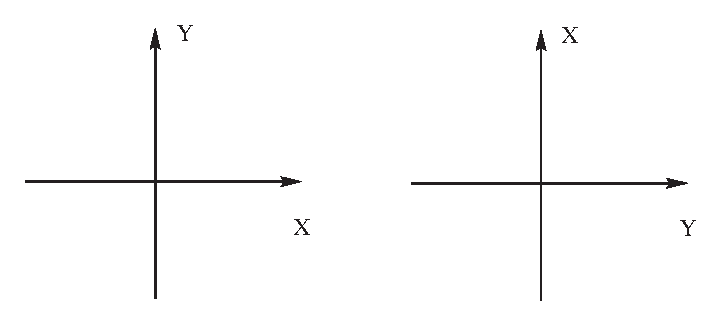
\includegraphics[scale=0.7]{coordinate_change.eps}
    \caption{coordinate changes by the $\sigma_{d}$} \label{GROUP12}
  \end{center}
\end{figure}

In the original coordinate system, the effects for both of $C^{1}_{4}$
and $C^{3}_{4}$ are:
\begin{eqnarray}
  % \nonumber to remove numbering (before each equation)
  C^{1}_{4}(z)[x,y] &\Rightarrow& [y,-x] \nonumber \\
  C^{3}_{4}(z)[x,y] &\Rightarrow& [-y,x]
\end{eqnarray}
Here it has a third symmetry operation of $\sigma_{d}$, which exchange
$x$ and $y$ ($\sigma_{d}[x,y] \Rightarrow [y,x]$).  Therefore, in the
new coordinate system indicating by the figure of (\ref{GROUP12}), we
have:
\begin{eqnarray}
  % \nonumber to remove numbering (before each equation)
  C^{1}_{4}(z)[x,y] \Leftrightarrow C^{1}_{4}(z)[y,x] (\text{old system})
  &\underrightarrow{\sigma_{d}}& [-y,x] \nonumber \\
  C^{3}_{4}(z)[x,y] \Leftrightarrow C^{3}_{4}(z)[y,x] (\text{old system})
  &\underrightarrow{\sigma_{d}}& [y,-x]
\end{eqnarray}
Thus, the $C^{1}_{4}$ and $C^{3}_{4}$ are equivalent symmetry
operations.

%%%%%%%%%%%%%%%%%%%%%%%%%%%%%%%%%%%%%%%%%%%%%%%%%%%%%%%%%%%%%%%%%%%%%%%%%%%%%%
\subsection{Class in point group}
%
% this section provide the details related to variety of the
% equivalent symmetry operation
%
So far we have fully understand the meaning of conjugation in the
point group. Now we can make some summarization that what kind of
symmetry operations are equivalent:

\begin{enumerate}
\item the identical operation and inversion operation.
  \begin{itemize}
  \item Since the both of $E$ and $i$ has only one element, $E$ and
    $i$ are individual class respectively.
  \end{itemize}
\item reflection
  \begin{itemize}
  \item If there's some operation to exchange their reflection mirror,
    such reflections related to these mirrors are in same class.
  \end{itemize}
\item $C_{n}$ and $S_{n}$ axis
  \begin{itemize}
  \item If there has mirrors containing the axis, or it has the
    $C_{2}$ vertical to the axis; the $C^{i}_{n}$ and $C^{n-i}_{n}$
    fall into same class, so as the $S^{i}_{n}$.
  \end{itemize}
\end{enumerate}

Finally we can make some extra example of $C_{4v}$ to classify the
principle with the $C_{n}$ and $S_{n}$ axis. The $C^{1}_{4}$ and
$C^{3}_{4}$ are conjugated for there is a mirror vertical to the
$C_{4}$ axis.

%%%%%%%%%%%%%%%%%%%%%%%%%%%%%%%%%%%%
\subsection{Classification of point group}
%
% this section provides the example of the point group
%
%
In the following content, we are going to give the systematical method
classification of the point group. From now on, for any molecules; we
can specify which point group it belongs to. All the symmetry
characters related to the molecule, is wholly demonstrated by the
details defined in its point group. We will begin from the simplest
case until reach to the complex ones.

$C_{1}$ group: \\
Actually this is only identical operation (E) related to this kind of
molecule, see figure of (\ref{GROUP1}).
\begin{figure}[htp]
  \begin{center}
    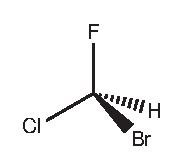
\includegraphics[scale=0.7]{molecule1.eps}
    \caption{C1 group} \label{GROUP1}
  \end{center}
\end{figure}

$C_{s}$ group: \\
$C_{s}$ is actually the group of $\sigma$; has two elements: $E$ and
$\sigma$, see figure of (\ref{GROUP2}).
\begin{figure}[htp]
  \begin{center}
    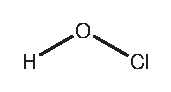
\includegraphics[scale=0.7]{molecule2.eps}
    \caption{CS group} \label{GROUP2}
  \end{center}
\end{figure}

$C_{n}$ group: \\
This group is identical to the group of $C_{n}$, only has a rotation
axis and identical operation, see figure of (\ref{GROUP3}).
\begin{figure}[htp]
  \begin{center}
    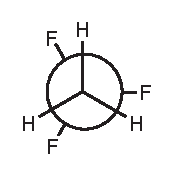
\includegraphics[scale=0.7]{molecule3.eps}
    \caption{C3 group} \label{GROUP3}
  \end{center}
\end{figure}

$C_{i}$ group: \\
This group is identical to the group of $i$, only has a inversion
operation and identical operation, see figure of (\ref{GROUP4}).
\begin{figure}[htp]
  \begin{center}
    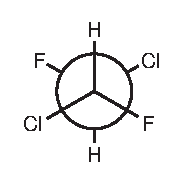
\includegraphics[scale=0.7]{molecule4.eps}
    \caption{Ci group} \label{GROUP4}
  \end{center}
\end{figure}

$S_{n}$ group: \\
From the content above, we know that $S_{4}$ is some individual
group. Here below we present one example in the figure of
(\ref{GROUP7}).
\begin{figure}[htp]
  \begin{center}
    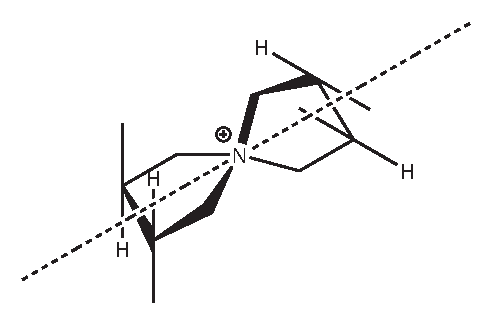
\includegraphics[scale=0.7]{S4_example.eps}
    \caption{S4 group} \label{GROUP7}
  \end{center}
\end{figure}

$C_{nv}$ group: \\
If we add a symmetry element of mirror to the $C_{n}$ axis, and this
mirror just contains the axis; from the analysis above we can know
that there must have n planes exist, as the rotation axis varies.
This group is called $C_{nv}$ group. The most famous example is
$H_{2}O$ molecule, see figure of (\ref{GROUP5}).
\begin{figure}[htp]
  \begin{center}
    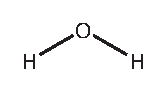
\includegraphics[scale=0.7]{molecule5.eps}
    \caption{C2v group} \label{GROUP5}
  \end{center}
\end{figure}

$C_{nh}$ group: \\
As what we have shown, This group is the direct product of the $C_{n}$
and $\sigma_{h}$, see figure of (\ref{GROUP6}).
\begin{figure}[htp]
  \begin{center}
    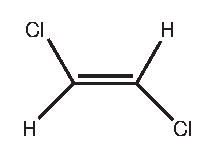
\includegraphics[scale=0.7]{molecule6.eps}
    \caption{Cnh group} \label{GROUP6}
  \end{center}
\end{figure}

$D_{n}$ group: \\
If we add $C_{2}$ axis to the $C_{n}$ axis, and the $C_{2}$ axis is
vertical to the $C_{n}$ axis; from the product principle above we can
know that there must have n $C_{2}$ axes as the $C_{n}$ axis
rotates. This situation is similar to the $C_{nv}$, actually they are
isomorphic groups, see figure of (\ref{GROUP8}).
\begin{figure}[htp]
  \begin{center}
    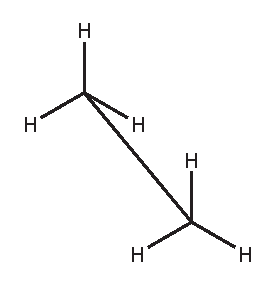
\includegraphics[scale=0.7]{molecule8.eps}
    \caption{D3 group} \label{GROUP8}
  \end{center}
\end{figure}

$D_{nh}$ group: \\
$D_{nh}$ group is produced by adding a $\sigma_{h}$ to the $D_{n}$
group, where the $\sigma$ is vertical to the main $C_{n}$ axis.  Since
we have n $C_{2}$ axes vertical to the $C_{n}$ axis, so the mirror
formed by the $\sigma_{h}$ embraces the n $C_{2}$ axes, thus we have
another n $\sigma_{v}$ containing the $C_{n}$ axis.  Besides, we have
the inversion point due to the cross of $C_{n}$ and $\sigma_{h}$. This
group is $D_{nh}$. The benzene molecule is one of this type, see
figure of (\ref{GROUP10}).
\begin{figure}[htp]
  \begin{center}
    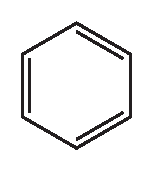
\includegraphics[scale=0.7]{molecule10.eps}
    \caption{benzene molecule of D6h group} \label{GROUP10}
  \end{center}
\end{figure}

$D_{nd}$ group: \\
In the $D_{nh}$ group, if the added in $\sigma_{h}$ is replaced by the
$\sigma_{d}$, which covers the main $C_{n}$ axis and split the
rotation angle into half in equal; this group we called $D_{nd}$
group, see figure of (\ref{GROUP9}).
\begin{figure}[htp]
  \begin{center}
    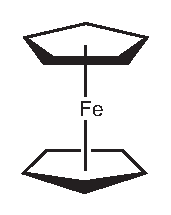
\includegraphics[scale=0.7]{molecule9.eps}
    \caption{D5d group} \label{GROUP9}
  \end{center}
\end{figure}

In this list, we omit all the more complicated cases, they are
containing more than one $C_{n}$ axes; such as the $CH_{4}$ molecule,
it has four $C_{3}$ axes. The more details can be found in the book
listed in reference\cite{Bishop, Cotton}.

%%%%%%%%%%%%%%%%%%%%%%%%%%%%%%%%%%%%%%%%%%%%%%%%%%%%%%%%%%%%%%%%%%%%%%%%%%%%
\section{Matrix representation of point group}

\subsection{What's the representations?}
%
% 1 explain what's the representations, however; in a example way to
% show this 2 detailed example to show what's the representation.  3
% general definition. the symmetry operation always has a matrix to
% express it on a given representation
%
In the above content, we have generally introduce the concept of
symmetry operation. However, what does the symmetry operation derive
from? That's what we call the ``representations'' (that's same to the
``base'' concept as in the discussion of section (\ref{GROUP13})).

Now let's give some example. For simplicity, we choose the $C_{4}$
(which contains the $C^{1}_{4}, C^{2}_{4}, C^{3}_{4}, E$ symmetry
operations) point group and try to give their corresponding
representations.

The first example is the most plain one. We can choose an arbitrary
point of $(x,y,z)$ to be the representation. Here, each of the
symmetry operation in the $C_{4}$ is embodied as a three dimensional
matrix, which is to describe the transformation of the point from one
position to another:
\begin{equation}\label{}
  \begin{bmatrix}
    \cos \frac{2i\pi}{4} & \sin \frac{2i\pi}{4} & 0 \\
    -\sin \frac{2i\pi}{4} & \cos \frac{2i\pi}{4} & 0 \\
    0                   & 0                   & 1 \\
  \end{bmatrix}
  \begin{bmatrix}
    x \\
    y \\
    z \\
  \end{bmatrix}
  =
  \begin{bmatrix}
    x^{'} \\
    y^{'} \\
    z^{'} \\
  \end{bmatrix}
\end{equation}
Here the matrix shown above represents the $C^{i}_{4}$ symmetry
operation in the given representation. Here we note that The rotation
axis is set to the Z direction.

This simple example can be extended to some more complicated form.  If
we consider some molecules, for instance, the $Ni(CO)_{4}$; it holds a
$C_{4}$ axis. Suggest that this molecule is putting on to the $XY$
plane then the rotation of $C^{i}_{4}$ can be clearly defined as the
counter-clock rotation around the $Z$ axis. Therefore if we consider
the coordinates of the atoms, then such rotation will be accordingly
some $27\times 27$ matrix describing the mixing states between the
atoms coordinates. A similar example can be found in Bishop's
book\cite{Bishop}, PP $94$.

On the other hand, we can strike up some other choices. For the
molecule of $Ni(CO)_{4}$, if we put the coordinate system on each atom
and keep the molecule unchanged(that's a bit different with the above
case, where we consider the coordinates of the atoms in a fixed
coordinate system); then for the $3\times 9=27$ vectors, we can also
find some matrix corresponding to the rotation operation of
$C_{4}^{i}$. Here, it's interesting to note that if we consider the
other molecules, which also holds the $C_{4}$ symmetry (for example,
$PtCl_{4}$ molecule; it's in a square shape); the representations will
also changed into other forms.

Moreover, the basis sets for the molecule of $Ni(CO)_{4}$ can also
form some representation. For example, the $6-31g(d,p)/Lanl2dz$ (here
the $Lanl2dz$ is used to describe the $Ni$ atom). For each of the
basis set, it actually forms some function space for the symmetry
operations of $C_{4}$; based on these function space, the $C_{4}$ can
be generalized to be some operators on the basis sets; yet in practice
it can be expressed into the transformation matrices to portray the
mixing states of the basis functions.

All in all, the representations is actually what we express the
symmetry operations on. It can be coordinates, basis sets, orbitals,
wave functions etc. There are unlimited ways to find the new form of
representations for a given symmetry operation (or a group of symmetry
operations). Among each of the concrete representation, we can always
find a way to express the abstract symmetry operation into some matrix
form, to fully express the symmetric property. Such matrices are
isomorphic to the given symmetry operations, in fact; these matrices
mirrors the symmetry operations are the most crucial link between the
symmetry of a molecule and its practical properties such as the
spectral character.

In Bishop's book\cite{Bishop}, the author offers sufficient discussion
about how to express a certain symmetry operation by variety of
representations. It's the best material for the further reading.

%%%%%%%%%%%%%%%%%%%%%%%%%%%%%%%%%%%%%%%%%%%%%%%%%%%%%%%%%%%%%%%%%%%%%%%%%%%
\subsection{Equivalent representations}
%
% 1 take the mathematical form 2 express the relation between two
% selected representations 3 to express the symmetry operation, to get
% the similarity transformation similarity transformation does not
% hurt the multiplication rules, that's why the selected
% representations are equivalent 4 so that we can always choose the
% unitary representation
%
From this section, we are going to study the characters related to the
matrix representation. The first we consider, is the equivalent
property.

Here it's more clear to introduce the idea of the equivalent
representation on mathematical form, rather than to introduce its
physical meanings. From the derivation below, the physical meaning is
quite clear.

First, let's consider some representations, it can be formed by the
basis sets, or the coordinates of atoms; now we choose the function
space as the example. Suggesting we have two sets of functions below:
\begin{align}\label{}
  f_{1}, f_{2}, f_{3}, &\cdots, f_{n} \nonumber \\
  g_{1}, g_{2}, g_{3}, &\cdots, g_{n}
\end{align}
These $n$-dimensional function space can be got from the result HF
orbitals, or the original basis sets. It's assumed that they express
the same function space, thus we can use an matrix transformation to
linking them together:
\begin{align}\label{}
  f_{i} &= \sum_{j}A_{ij}g_{j} \quad (j=1,2,\cdots, n) \nonumber \\
  g_{k} &= \sum_{j}B_{kj}f_{j} \quad (j=1,2,\cdots, n)
\end{align}
For the $A$ and $B$ we have:
\begin{align}\label{}
  f_{i} &= \sum_{j}A_{ij}(\sum_{l}B_{jl}f_{l}) \nonumber \\
  &= \sum_{j}\sum_{l}A_{ij}B_{jl}f_{l} \Rightarrow \nonumber \\
  &\sum_{j}A_{ij}B_{jl} = \delta_{il}
\end{align}
So we have $AB=E$. On the other hand, we can prove that $BA=E$. So
$A=B^{-1}$.

Then we consider the operator of $\hat{O}_{R}$ (it corresponds to the
symmetry operation of R), for both of the $f$ and $g$ bases, we can
have:
\begin{align}\label{}
  \hat{O}_{R} f_{i} &= \sum_{k=1}^{n}D^{f}_{ik}(R)f_{k} \nonumber \\
  \hat{O}_{R} g_{i} &= \sum_{j=1}^{n}D^{g}_{ij}(R)g_{j}
\end{align}
The $D$ denotes the transformation matrix for the $\hat{O}_{R}$.

Now we have:
\begin{align}\label{}
  \hat{O}_{R} g_{i} &= \hat{O}_{R}(\sum_{j}B_{ij}f_{j}) \nonumber \\
  &= \sum_{j}B_{ij}(\hat{O}_{R}f_{j}) \nonumber \\
  &= \sum_{j}B_{ij}(\sum_{k=1}^{n}D^{f}_{jk}(R)f_{k})\nonumber \\
  &= \sum_{j}B_{ij}\sum_{k=1}^{n}D^{f}_{jk}(R)(\sum_{l}A_{kl}g_{l})
  \nonumber \\
  &=(\sum_{j}B_{ij}\sum_{k=1}^{n}D^{f}_{jk}(R)\sum_{l}A_{kl})g_{l}
  \nonumber \\
\end{align}
Therefore, we have:
\begin{equation}\label{}
  D^{g}_{il}(R) =
  \sum_{j=1}^{n}\sum_{k=1}^{n}B_{ij}D^{f}_{jk}(R)A_{kl}
\end{equation}
or express in a matrix form:
\begin{equation}\label{}
  D^{g}(R) = BD^{f}(R)A = BD^{f}(R)B^{-1}
\end{equation}

Here we note that in the above deduction, the base of $f$ and $g$ are
manipulated all by the column; that is:
\begin{equation}\label{}
  \sum_{j}A_{ij}g_{j} \Leftrightarrow
  \begin{bmatrix}
    A_{11} & \cdots & A_{1n} \\
    \cdots & \cdots & \cdots \\
    A_{n1} & \cdots & A_{nn} \\
  \end{bmatrix}
  \begin{bmatrix}
    g_{1}  \\
    \cdots \\
    g_{n}  \\
  \end{bmatrix}
\end{equation}

All in all, the above derivation shows that the $f$ and $g$ are
associated with each other by some similarity transformation. On this
condition, $f$ and $g$ are called ``equivalent'' representations.

It's easy to know that the similarity transformation does not alter
the multiplication rules, that is if we have $D^{f}(SR) =
D^{f}(S)D^{f}(R)$, for the $g$ basis it also has $D^{g}(SR) =
D^{g}(S)D^{g}(R)$. That's why we say such basis are equivalent. This
is the final conclusion we get.

For this reason, it's safe to choose some special form of
representations, which is the most suitable one to deal with
question. It can prove that among the equivalent expressions, it can
always choose the unitary matrices without hurting the universality.
Hence in the following content, the unitary matrices is chosen to
express the specific symmetry operations or the point group.

%%%%%%%%%%%%%%%%%%%%%%%%%%%%%%%%%%%%%%%%%%%%%%%%%%%%%%%%%%%%%%%%%%%%%%%%%%%%%%
\subsection{Reducible and irreducible representations}
%
% 1 introduce the Gamma to represent the representation wholly 2
% introduce the concept of reducible representation 3 discussion
% related to the counter operation 4 reducible and irreducible
% concepts 5 the relations between reducible and irreducible
% representations
%
Now it's the time to introduce the symbol of ``$\Gamma$'' to express
all the matrices in a given group (as we note above, in a specific
representation each matrix corresponds to some symmetry operation) for
a given representation. Here, $\Gamma$ is not representing one single
matrix but all the matrices in a given group constituting the given
representation. The introduction of such concept is used to depict the
irreducible and reducible character, which are related to all the
matrices within a given group.

Suggesting we have a set of base of $f_{i}$ ($i=1,2,\cdots, n$). If
for each of the symmetry operation of $\hat{O}_{R}$ in the given
group, we have the relations below:
\begin{align}\label{}
  \hat{O}_{R}f_{1} &= D_{11}(R)f_{1} + \cdots + D_{m1}(R)f_{m} +
  0f_{m+1} + \cdots + 0f_{n} \nonumber \\
  \hat{O}_{R}f_{2} &= D_{12}(R)f_{1} + \cdots + D_{m2}(R)f_{m} +
  0f_{m+1} + \cdots + 0f_{n} \nonumber \\
  \cdots & \cdots \cdots \cdots \nonumber \\
  \hat{O}_{R}f_{m} &= D_{1m}(R)f_{1} + \cdots + D_{mm}(R)f_{m} +
  0f_{m+1} + \cdots + 0f_{n} \nonumber \\
  \hat{O}_{R}f_{m+1} &= 0f_{1} + \cdots + 0f_{m} +
  D_{m+1, m+1}(R)f_{m+1} + \cdots + D_{n,m+1}(R)f_{n} \nonumber \\
  \hat{O}_{R}f_{m+2} &= 0f_{1} + \cdots + 0f_{m} +
  D_{m+1, m+2}(R)f_{m+1} + \cdots + D_{n,m+2}(R)f_{n} \nonumber \\
  \cdots & \cdots \cdots \cdots \nonumber \\
  \hat{O}_{R}f_{n} &= 0f_{1} + \cdots + 0f_{m} +
  D_{m+1, n}(R)f_{m+1} + \cdots + D_{n,n}(R)f_{n} \nonumber \\
\end{align}

Here we can see that the above equation shows that for each of the
matrix in the representation, it has the form below:
\begin{equation}
  D(R) \Leftrightarrow \left(
    \begin{array}{cc}
      D^{1}(R) & 0        \\
      0        & D^{2}(R) \\
    \end{array}
  \right)
\end{equation}
In the above example, the $D^{1}(R)$ is $m$-dimensional, the the
$D^{2}(R)$ is $n-m$-dimensional.

According to the discussion above, we can choose the unitary form of
the matrices to express the symmetry operation of R. Thus, for its
counter operation of $R^{-1}$, we have:
\begin{equation}\label{}
  D(R^{-1}) = D(R)^{+} =\left(
    \begin{array}{cc}
      D^{1}(R)^{+} & 0        \\
      0        & D^{2}(R)^{+} \\
    \end{array}
  \right)
\end{equation}
Therefore, the counter operation also holds the block form.

For the $\Gamma$, if there's some way to change all the matrices in
this representation into such block form, then this $\Gamma$ is
reducible; else it's irreducible.

For the $D(R)$ in reducible suggest that $\Gamma_{1}$ has the form
below:
\begin{equation}\label{}
  D(R)       = \begin{vmatrix}
    D^{1}(R) & 0        & 0        \\
    0        & D^{2}(R) & 0        \\
    0        & 0        & D^{3}(R) \\
  \end{vmatrix}
\end{equation}
IT's easy to prove that if we have $D(Q) = D(R)D(S)$, then for each of
the $D^{i}(R)$, it also has $D^{i}(Q) = D^{i}(R)D^{i}(S)$.  Different
$D^{i}(R)$ never mix with each other. Therefore, the blocks in the
reducible representation of $D^{i}(R)$ also fully corresponds to the
given symmetry operations or point group (additionally, the
representations behind the block matrix of $D^{i}(R)$ is sufficient to
be some independent representations). In this sense, it's said that
the reducible representation is the ``direct sum'' of the irreducible
representations, all of the characters inside the reducible
representation is wholly determined by its irreducible components.

For this reason, the reducible representation can be expressed as:
\begin{equation}\label{}
  \Gamma = \Gamma^{1} \bigoplus \Gamma^{2} \bigoplus \Gamma^{3}
\end{equation}
If some $\Gamma^{i}$ appears many times, we can also write:
\begin{equation}\label{}
  \Gamma = a_{1}\Gamma^{1} \bigoplus a_{2}\Gamma^{2} \bigoplus
  a_{3}\Gamma^{3}
\end{equation}

%%%%%%%%%%%%%%%%%%%%%%%%%%%%%%%%%%%%%%%%%%%%%%%%%%%%%%%%%%%%%%%%%%%%%%%%%%%
\section{Great orthogonality theorem}
%
%
%
In the application of the group theory in chemistry, there has a
theorem which possesses the key position in the whole theory; that's
the the great orthogonality theorem; or the key theorem. This theorem
describe the relationship between the matrix elements among the
irreducible representations, however; the deep study will show that
it's a connection between the properties of abstract symmetry
operation and its corresponding representation matrices. In this
section, we are going to give a detailed study around this subject.


%%%%%%%%%%%%%%%%%%%%%%%%%%%%%%%%%%%%%%%%%%%%%%%%%%%%%%%%%%%%%%%%%%%%%%%%%%%%%%%
\subsection{The key theorem}
%
% 1 to show this theorem 2 transform it to the unitary matrices form 3
% make a bit of analysis 4 show the reason that why we consider the
% characters
%
First let's state the key theorem. Here for simplicity the proof is
omitted, but it can found in the Bishop's book\cite{Bishop}.

Suggest we have a point group. For every symmetry operations of R in
this point group, we introduce two irreducible representations of
$\Gamma^{\mu}$ and $\Gamma^{\nu}$ (the matrices are labeled as
$D^{\mu}(R)$ and $D^{\nu}(R)$, separately). Here, the key theorem
states that for the elements of $D^{\mu}(R)$ and $D^{\nu}(R)$, they
satisfy the relations below:
\begin{equation}\label{GROUPeq:15}
  \sum_{R}D^{\mu}_{ik}(R) D^{\nu}_{mj}(R^{-1}) =
  (g/n_{\mu})\delta_{\mu\nu} \delta_{ij} \delta_{km}
\end{equation}

Since that we can always take the unitary matrix form, we can rewrite
the theorem as:
\begin{align}\label{}
  \sum_{R}D^{\mu}_{ik}(R) D^{\nu}_{mj}(R^{-1}) &=
  \sum_{R}D^{\mu}_{ik}(R) D^{\nu}_{mj}(R)^{+} \nonumber \\
  &= \sum_{R}D^{\mu}_{ik}(R) D^{\nu}_{jm}(R)^{*} \nonumber \\
  &= (g/n_{\mu})\delta_{\mu\nu} \delta_{ij} \delta_{km}
\end{align}

Thus, the final form below is what we always refer to.
\begin{equation}\label{GROUPeq:16}
  \sum_{R}D^{\mu}_{ik}(R) D^{\nu}_{jm}(R)^{*} =
  (g/n_{\mu})\delta_{\mu\nu} \delta_{ij} \delta_{km}
\end{equation}

Now we are going to make a bit of analysis. For the $\Gamma^{\mu}$,
each symmetry operation of R will give a matrix, which contains
$n_{\mu}^{2}$ elements. If we loop over all the symmetry operations R
(suggest we have $g$ symmetry operations in this point group), the
matrix element of $D_{ij}(R)$ will form a $g$-dimensional vector; such
vectors is in total number of $n_{\mu}^{2}$. From the equation of
(\ref{GROUPeq:16}), we can see that these vectors are orthogonal with
each other. Furthermore, since that different representations are also
orthogonal with each other, we can imagine that we can construct a
matrix similar like this:
\begin{equation}\label{}
  \begin{vmatrix}
    D_{11}^{\mu}(R_{1})             & D_{11}^{\mu}(R_{2})             & \cdots &  D_{11}^{\mu}(R_{g})              \\
    D_{12}^{\mu}(R_{1})             & D_{12}^{\mu}(R_{2})             & \cdots &  D_{12}^{\mu}(R_{g})              \\
    \cdots                          & \cdots                          & \cdots &  \cdots                           \\
    D_{n_{\mu}n_{\mu}}^{\mu}(R_{1}) & D_{n_{\mu}n_{\mu}}^{\mu}(R_{2}) & \cdots &  D_{n_{\mu}n_{\mu}}^{\mu}(R_{g})  \\
    D_{11}^{\nu}(R_{1})             & D_{11}^{\nu}(R_{2})             & \cdots &  D_{11}^{\nu}(R_{g})              \\
    D_{12}^{\nu}(R_{1})             & D_{12}^{\nu}(R_{2})             & \cdots &  D_{12}^{\nu}(R_{g})              \\
    \cdots                          & \cdots                          & \cdots &  \cdots                           \\
    D_{n_{\nu}n_{\nu}}^{\nu}(R_{1}) & D_{n_{\nu}n_{\nu}}^{\nu}(R_{2}) & \cdots &  D_{n_{\nu}n_{\nu}}^{\nu}(R_{g})  \\
    \cdots                          & \cdots                          & \cdots &  \cdots                           \\
  \end{vmatrix}
\end{equation}
This matrix totally has $\sum n_{\mu}^{2}$ rows, but has only $g$
columns. Thus it leads to conclusion:
\begin{equation}\label{}
  \sum n_{\mu}^{2} \leq g
\end{equation}
Further proof shows that
\begin{equation}\label{}
  \sum n_{\mu}^{2} = g
\end{equation}

Therefore, it limits the number and dimension of irreducible
representations for a given point group.

However, the great orthogonality theorem is complicated so that
difficult to get more valuable information. For this reason, we
introduce the concept of ``character'' to re-express this theorem.  At
that moment we can see the clear expression will lead to more fruitful
results.

%%%%%%%%%%%%%%%%%%%%%%%%%%%%%%%%%%%%%%%%%%%%%%%%%%%%%%%%%%%%%%%%%%%%%%%%%%%%
\subsection{Character}
%
% 1 introduce the trace concept 2 for the symmetry operations in the
% same class, their corresponding matrices have the same characters.
% 3 rewrite the key theorem by the characters
%
%
From the algebra, the trace of a matrix is its sum of diagonal
elements:
\begin{equation}\label{}
  Trace(A) = \sum_{i} A_{ii}
\end{equation}
It's well known that the trace does not change between the similarity
transformations. Thus, we introduce the concept of character, which is
is the trace of representation matrix (it's labeled as $\chi$):
\begin{equation}\label{}
  \chi^{\mu}(R) = Trace(D^{\mu}(R))
\end{equation}

Now let's say more about related to the characters. First we can prove
that for the symmetry operations in the same class, their
corresponding matrices have the same characters.

This is easy to understand. Suggest we have symmetry operations of $P$
and $Q$, which has the relations:
\begin{equation}\label{}
  X^{-1}PX = Q
\end{equation}
Then the corresponding matrix satisfy (for the $\mu$ representation):
\begin{equation}\label{}
  D^{\mu}(X)^{-1}D^{\mu}(P)D^{\mu}(X) = D^{\mu}(Q)
\end{equation}
Thus P and Q are connected by some similarity transformation, so
directly we can get:
\begin{equation}\label{}
  \chi(P) = \chi(Q)
\end{equation}

Thus for a given representation, the character for the symmetry
operation within a class is same. Similarly, by the same way we can
get that the equivalent representations share the same characters for
each of the symmetry operation (because they are associated with each
other by the similarity transformation, too). Hence, it's worthy to
note that through the concept of ``character'', now the ``class'' and
the ``equivalent representations'' are connected together.

Furthermore, we can use the character to rewrite the great
orthogonality theorem. From the (\ref{GROUPeq:16}), we can have:
\begin{eqnarray}\label{GROUPeq:9}
  % \nonumber to remove numbering (before each equation)
  \sum_{R} D^{\mu}_{ii}(R) D^{\nu}_{jj}(R)^{*} &=&  (g/n_{\mu})\delta_{\mu\nu}
  \delta_{ij}  \nonumber \\
  \sum_{i}\sum_{j}\sum_{R} D^{\mu}_{ii}(R) D^{\nu}_{jj}(R)^{*} &=&
  (g/n_{\mu})\delta_{\mu\nu}\sum_{i}\sum_{j}\delta_{ij}  \nonumber \\
  \sum_{R}\chi^{\mu}(R)\chi^{\nu}(R)^{*} &=&  g\delta_{\mu\nu}
\end{eqnarray}
Then for the irreducible representation of $\Gamma^{\mu}$, the
$\chi^{\mu}(R)$ ($R = R_{1}, R_{2}, \cdots, R_{g}$) is composed into
some $g$-dimensional vector; and here the vectors from different
representations are orthogonal with each other.

Next we are going to show how to express the concept of class in the
key theorem. Now for a given point group, each class inside we label
it as $C_{i}$ (here it should not mix with the n axis of $c_{n}$), the
number of the classes is $k$, the number of all the symmetry
operations is $g$, and the number of symmetry operations within each
class is $g_{i}$. So we have: $\sum_{i=1}^{k} g_{i} = g$.

For example, to the point group of $C_{3v}$; we have:
\begin{align}\label{}
  C_{1} &: E \nonumber \\
  C_{2} &: \sigma_{1}, \sigma_{2}, \sigma_{3} \nonumber \\
  C_{3} &: c^{1}_{3},c^{2}_{3}
\end{align}
Thus in the given example, $g=6$, $k=3$. Since that in each class of
$C_{i}$, the character keep to be same; so we can write the
(\ref{GROUPeq:9}) as:
\begin{equation}\label{}
  \sum_{i=1}^{k}g_{i}\chi^{\mu}(C_{i})\chi^{\nu}(C_{i})^{*} =
  g\delta_{\mu\nu}
\end{equation}

Furthermore, the above equation can be rearranged as:
\begin{equation}\label{}
  \sum_{i=1}^{k}\{g_{i}^{\frac{1}{2}}\chi^{\mu}(C_{i})\}
  \{g_{i}^{\frac{1}{2}}\chi^{\nu}(C_{i})^{*}\}
  = g\delta_{\mu\nu}
\end{equation}
Now it can see that the $g_{i}^{\frac{1}{2}}\chi^{\mu}(C_{i})$ has
formed as some $k$-dimensional vectors, and they are orthogonal with
each other if they come from different representations. Each one
represents the specific character for the class.

Therefore, we can see that the number of irreducible representations
should be less than the number of class:
\begin{equation}\label{}
  r \leq k
\end{equation}
The more strict proof demonstrates that actually the equality is
archived:
\begin{equation}\label{}
  r = k
\end{equation}
Finally, we can see that the number of irreducible representations
should equal to the number of classes in the point group.

%%%%%%%%%%%%%%%%%%%%%%%%%%%%%%%%%%%%%%%%%%%%%%%%%%%%%%%%%%%%%%%%%%%%%%%%%%%
\subsection{Clarification about the representations}
%
% clarify the concept between the equivalent representations and the
% class give some example to show how to understand the conclusion got
% from the above content.
%

Although it's very easy to distinguish literally the concept of
equivalent representations and the concept of ``class'' in the
symmetry operations, however I find that their mathematical
expressions always puzzle me. Thus in this passage I hope to give a
thorough discussion to it.

As we have known, the equivalent representations share the same
characters, that means for each of symmetry operation in the given
point group, the matrix of $D^{k}(R_{i})$ formed from the specific
representation $k$ ($i = 1, 2, \cdots, n$) shares the same character
of $D^{k^{'}}(R_{i})$ in the representation of $k^{'}$.

On the other hand, the concept of class is expressed based on the
different things. For a specific representation of $k$, they symmetry
operations are grouped in classes; for each class the matrices share
the same characters.

Hence, it turns out that they are two different things. However, the
great orthogonality theorem bridges them together, by requiring that
the number of non-equivalent irreducible representations should be the
same to the number of classes in a given point group. That means, for
any representations; if it's irreducible, it only belongs to several
kinds restricted by the number of class (else it must be equivalent to
some other irreducible representations); if it's reducible, that
there's only several kinds of non-equivalent irreducible
representations can be found, the other irreducible representations
must be equivalent to them.

Now let's give some example. For the molecule with the $C1$ symmetry,
it only has one class that contains only symmetry operation of $E$,
thus there's only one non-equivalent irreducible representation, in
the later concept we can see such representation is labeled as
$A$. Hence no matter how many molecule orbitals we have, for the $C1$
molecule we can only get the $A$ type of orbitals.

Similarly, for the point group of $C2v$, we have $4$ classes then we
must has only $4$ kinds of non-equivalent irreducible
representations. Actually these four non-equivalent irreducible
representations are characterized by $A_{1}$, $A_{2}$, $B_{1}$ and
$B_{2}$. Hence for the molecule possesses the $C2v$ symmetry, their
orbitals must fall into these four kinds.

%%%%%%%%%%%%%%%%%%%%%%%%%%%%%%%%%%%%%%%%%%%%%%%%%%%%%%%%%%%%%%%%%%%%%%%%%%%
\subsection{Evaluate the number of irreducible representations in the
  reducible one}
%
% 1 the equation of evaluating the number of irreducible
% representations from the reducible one 2 to prove the theorem that
% any two representations, if they share the same character arrays;
% then they must be equivalent.
%
Now let's consider an reducible representation of $\Gamma^{red}$, it
can be expressed by:
\begin{equation}\label{}
  \Gamma^{red} = \sum_{i=1}^{k}a_{i}\Gamma^{i}
\end{equation}
Here $\Gamma^{i}$ denotes to the non-equivalent irreducible
representation, from the discussion above we can know that only these
representations are meaningful in the reducible ones. The $k$ denotes
to the number of classes.

On the other hand, it's much more natural to rewrite the above
equation by the character:
\begin{equation}\label{}
  \chi^{red}(R) = \sum_{i=1}^{k}a_{i}\chi_{i}(R)
\end{equation}
From this expression, the meaning of using non-equivalent irreducible
representation is more clear since that different non-equivalent
irreducible representation will get different character array (if we
take all the symmetry operations of R into consideration, the
characters are forming an array; and arrays from different
non-equivalent irreducible representation are orthogonal with each
other).

Now by multiplying the $\chi_{j}^{*}(R)$ to the above equation, we can
have:
\begin{align}\label{}
  \sum_{R}\chi^{red}(R)\chi_{j}^{*}(R) &=
  \sum_{R}\sum_{i=1}^{k}a_{i}\chi_{i}(R)\chi_{j}^{*}(R) \nonumber \\
  &=\sum_{i=1}^{k}a_{i}g\delta_{ij} \nonumber \\
  &= ga_{i}
\end{align}

That yields some useful equation:
\begin{equation}\label{GROUPeq:1}
  a_{i} = \frac{1}{g}\sum_{R}\chi^{red}(R)\chi_{i}^{*}(R)
\end{equation}

From the previous discussion, we have known that if two
representations are equivalent, they will give the same character
arrays formed by the symmetry operations of $R_{i}$ ($i=1,2,\cdots,
n$).

Now based on the equation of (\ref{GROUPeq:1}), we can prove its
inverse proposition that if the character arrays are same between two
representations, then they must be equivalent.

First, suggest two irreducible representations; there will be two
situations: one is that they are non-equivalent, then the character
arrays formed must be orthogonal; the other case is that they are
equivalent, then the character arrays formed must be same (since for
each symmetry operation both of the representation matrices has the
same characters).

Second, for two representations which are reducible; let's consider
their character arrays formed by the non-equivalent irreducible
representations (equivalent ones get the same character arrays so that
they are needed to take into account). If the two reducible
representations have the same character arrays, it can see that they
must have the same type of non-equivalent irreducible
representations. Then according to the equation of (\ref{GROUPeq:1}),
their number must be same. Thus, we can rearrange the non-equivalent
irreducible representations of $\Gamma^{i}$ so that to make the two
reducible representations same. Therefore, for any two
representations, if they share the same character arrays; then they
must be equivalent.

%%%%%%%%%%%%%%%%%%%%%%%%%%%%%%%%%%%%%%%%%%%%%%%%%%%%%%%%%%%%%%%%%%%%%%%%%%%%%
\subsection{Criteria for irreducibility}
%
%
% how to judge a given representation is reducible or not
%
%
Now we can judge a given representation is reducible or not based on
the (\ref{GROUPeq:9}). Suggest for some representation we have:
\begin{equation}\label{}
  \chi^{a}(R) = \sum_{i=1}^{k_{1}}a_{i}\chi_{i}(R)
\end{equation}
Then we have:
\begin{align}\label{}
  \sum_{R}\chi^{a}(R)\chi^{a}(R)^{*} &=
  \sum_{R}\sum_{i=1}^{k_{1}}a_{i}\chi_{i}(R)\sum_{j=1}^{k_{1}}a_{j}\chi_{j}(R)^{*} \nonumber \\
  &=\sum_{i=1}^{k_{1}}a_{i}\sum_{j=1}^{k_{1}}a_{j}\sum_{R}\chi_{i}(R)\chi_{j}(R)^{*} \nonumber \\
  &= g\sum_{i=1}^{k_{1}}\sum_{j=1}^{k_{1}}a_{i}a_{j}\delta_{ij} \nonumber \\
  &= g\sum_{i=1}^{k_{1}}a_{i}^{2}
\end{align}

If $\chi^{a}$ represents some irreducible representation, then it can
only has one component of $a_{i}$, other items will go to be
zero. Then we have:
\begin{equation}\label{GROUPeq:5}
  \sum_{R}\chi^{a}(R)\chi^{a}(R)^{*}  = g
\end{equation}
Therefore the (\ref{GROUPeq:5}) indicates that if the representation
is irreducible, then the inner product of the corresponding character
array will be a number of $g$.

%%%%%%%%%%%%%%%%%%%%%%%%%%%%%%%%%%%%%%%%%%%%%%%%%%%%%%%%%%%%%%%%%%%%%%%%%%%%%
\subsection{Character Table}
%
% 1 why do we have the character table 2 mulliken symbol 3 how to
% understand the non-equivalent irreducible representations
%

From the discussion above, we can see that the character for each
point group are unique, it's one-to-one mapping with the
non-equivalent irreducible representations; in other words, it
characterizes the non-equivalent irreducible representations for a
given point group. Since that the characters for the non-equivalent
irreducible representations only depend on the class of symmetry
operations, and irrelevant to what concrete representations we choose;
then it's possible to construct the character table. Below there's a
typical character table for $C_{3v}$:

\begin{center}
  \begin{tabular}{c|c c c|c|c}
    % after \\: \hline or \cline{col1-col2} \cline{col3-col4} ...
    $C_{3v}$ & $E$ & $2C_{3}$ & $3\sigma_{v}$ &                          &    \\
    \hline
    $A_{1} $ & 1   &     1    &      1        & $z$                      &
    $x^{2}+y^{2}$, $z^{2}$ \\
    $A_{2} $ & 1   &     1    &     -1        & $R_{z}$                  &    \\
    $E$      & 2   &    -1    &      0        & $(x,y)$, $(R_{x},R_{y})$ &
    $(x^{2}-y^{2}, xy)$, $(xz, yz)$ \\
  \end{tabular}
\end{center}

Now by the example of $C_{3v}$, we are going to give some illustration
about how to understand the character table.

As we can see, the character table can be divided into four blocks and
each one is separated from the others by the vertical line.

In the first block, there's the label for the non-equivalent
irreducible representations. The designation for these representations
are brought up by Mulliken, so it's also called Mulliken symbols. the
rule to draw the Mulliken symbols is:
\begin{itemize}
\item all the one dimensional representations are labeled as $A$ or
  $B$, two dimensional representations are labeled as $E$; and three
  dimensional representations are labeled as $T$ or $F$.
\item for the one dimensional representation, if it has the $C_{n}$
  axis ($n \geq 2$), the symbol of $A$ or $B$ is decided by the state
  of character for the highest order of $C^{1}_{n}$; if it's $+1$,
  then the label of $A$ is used; if $-1$ the label of $B$ is used.
\item for the $C_{1}$, $C_{i}$ and $C_{s}$ type of molecule, they all
  labeled as $A$.
\item If the molecule has $C_{2}$ axis or the mirrors containing the
  $C_{n}$ axis; the subscript of $1$ or $2$ can be used to classify
  the case that whether the $C_{2}$ axis (or the mirrors) give the
  $+1$ character or the $-1$ character. If $+1$ then the subscript of
  $1$ is selected, else $2$ is chosen.
\item If the molecule has $\sigma_{h}$, then the symbol of $'$ or $''$
  indicate that the character for the $\sigma_{h}$ is $+1$ or $-1$.
\item If the molecule has symmetry operation of $i$, then the
  subscript of $g$ means the character for the $i$ operation is $+1$,
  and the subscript of $u$ means the character for the $i$ operation
  is $-1$.
\end{itemize}

The second block is the characters for each class. Formally they can
be constructed from the mathematical rules we mentioned in the above
content.

The third and fourth blocks are related to the ``base'' of the
representations. For example, if we choose one point coordinates of
$(x,y,z)$ to represent the point group of $C_{3v}$, then for each
symmetry operation we can get the corresponding matrix, that is the
representation; from such matrices we can see that the $z$ component
is never mixing with the $(x,y)$ by having the formation below:
\begin{equation}\label{}
  \begin{bmatrix}
    D(x,y) & 0    \\
    0      & D(z) \\
  \end{bmatrix}
\end{equation}
here the $D$ means small matrix inside the representation. Thus we can
see that the $z$ forms the one dimensional irreducible representation
for the $C_{3v}$, and the $(x,y)$ forms the two dimensional
irreducible representation for the $C_{3v}$ point group.  They are
non-equivalent, each one has its own character array.  That's what
these two blocks tell us.

Here we are going to omit the other detailed discussion of the
character table. The reader can consult the book by
Bishop\cite{Bishop} and Cotton\cite{Cotton} for more interesting
details.

%%%%%%%%%%%%%%%%%%%%%%%%%%%%%%%%%%%%%%%%%%%%%%%%%%%%%%%%%%%%%%%%%%%%%%%%%%%%
\subsection{Symmetry project operator}
%
% 1 why we want to construct the project operator?  2 derive the
% concrete expression for the project operator 3 how can we understand
% the operator 4 examples to show how to do the projection on the
% basis functions
%
In quantum chemistry, usually we will encounter a kind of problem that
to transform on function space of $F$ into another of $G$:
\begin{equation}\label{}
  f_{1}, f_{2}, \cdots, f_{n} \Rightarrow g_{1}, g_{2}, \cdots, g_{n}
\end{equation}
The new form of $G$ may possess some kind of benefit in calculation.
The symmetry project operator is able to perform this transformation
job.

For example, the $F$ may be originally selected as the basis functions
for some molecules we wish to study, usually they are the reducible
representations. However; if the molecule has symmetry then we can
make use of it. Before the concrete calculation, e.g. HF calculation;
we should organize the basis functions into its linear combination of
$G$ so that it can be the irreducible representations. In the latter
content, we can see that due to the vanishing integral rules that a
lot of calculations can be avoided by using the irreducible
representations.

Now we begin to derive the expression for the symmetry project
operator. Suggest we have some function space of $F$:
\begin{equation}\label{}
  f^{\nu}_{1}, f^{\nu}_{2}, f^{\nu}_{3}, \cdots, f^{\nu}_{n_{\nu}}
\end{equation}
this function space can be reducible or irreducible. After imposing on
the symmetry operator of $\hat{O}_{R}$, it gives:
\begin{equation}\label{GROUPeq:10}
  \hat{O}_{R}f^{\nu}_{p} =
  \sum_{q=1}^{n_{\nu}}D^{\nu}_{pq}(R)f^{\nu}_{q}
\end{equation}

For each of the symmetry operation of $R$, we can have the above
expression. Now we multiply the (\ref{GROUPeq:10}) with
$D^{\mu}_{ij}(R)^{*}$, and sum up all the symmetry operations of $R$;
according to the key theorem it gives:
\begin{align}\label{GROUPeq:11}
  \sum_{R}D^{\mu}_{ij}(R)^{*}\hat{O}_{R}f^{\nu}_{p} &=
  \sum_{q=1}^{n_{\nu}}\sum_{R}D^{\mu}_{ij}(R)^{*}
  D^{\nu}_{pq}(R)f^{\nu}_{q} \nonumber \\
  &=\sum_{q=1}^{n_{\nu}}(g/n_{\nu})\delta_{ip}
  \delta_{jq}\delta_{\mu\nu}f^{\nu}_{q} \nonumber \\
  &=(g/n_{\nu})\delta_{ip}\delta_{\mu\nu}f^{\nu}_{j}
\end{align}

Now we can define some new operator, which is taken the form below:
\begin{equation}\label{GROUPeq:12}
  P^{\mu}_{ij} = \sum_{R}D^{\mu}_{ij}(R)^{*}\hat{O}_{R}
\end{equation}
This is the symmetry project operator.

Now we wish to make some analysis based on the derivation on the
(\ref{GROUPeq:11}). Firstly, we can see that the project operator is
associated with the matrix element of $D^{\mu}(R)^{*}$ but not the
whole matrix; it's a very interesting feature that it implies some
possibility that the construction of the new function space does not
need the information of whole matrix, it's element is enough.

Secondly, it's only that $\mu$ and $\nu$ are some equivalent
irreducible representations then the element in the original function
space $F$ can be left behind, other elements which belongs to
different irreducible representations will be sweeped out. This is
also the reason that why we call the operator defined in the
(\ref{GROUPeq:12}) as ``project operator''.

Based on the above analysis, we can see the possibility to use the
trace to express the symmetry project operator. In (\ref{GROUPeq:12})
let's take the diagonal element ($i=j$) and sum over all the $i$, it
gives:
\begin{align}\label{}
  P^{\mu}=\sum_{i}P^{\mu}_{ii} &=
  \sum_{i}\sum_{R}D^{\mu}_{ii}(R)^{*}\hat{O}_{R} \nonumber \\
  &=\sum_{R}\sum_{i}D^{\mu}_{ii}(R)^{*}\hat{O}_{R} \nonumber \\
  &=\sum_{R}\chi^{*}(R)\hat{O}_{R}
\end{align}
In many cases it's much more useful than the (\ref{GROUPeq:12})
because that the character for the symmetry operation is easier to
get.

Finally let's give some example to show that how to use the symmetry
project operator to ``project'' new function space from the old one.
Take the $NH^{3}$ molecule as an example, it has three hydrogen atoms;
we take the $1s$ orbital(Gaussian orbitals, or Slater type; any is OK)
from each of the atoms, they are labeled as: $a$, $b$, $c$. It's known
to be the reducible representations. Now we wish to organize them into
the irreducible representations.

First let's select one of $1S$ hydrogen orbital, e.g. the orbital $a$;
then the symmetry operation of $R$ on the orbital $a$ gives:

\begin{center}
  \begin{tabular}{ c|c c c c c c }
    \hline
    % after \\: \hline or \cline{col1-col2} \cline{col3-col4} ...
    R   & E & $c^{1}_{3}$ & $c^{2}_{3}$ & $\sigma^{'}$
    & $\sigma^{''}$ & $\sigma^{'''}$ \\
    \hline
    R(a) & a & b & c & a & c & b \\
  \end{tabular}
\end{center}
The table above is derived from the intuitional observations.

Now we can see that in the (\ref{GROUPeq:11}) we have gotten the
$\hat{O}_{R}f^{\nu}_{p}$. now we consider the character table for the
$C_{3v}$:

\begin{center}
  \begin{tabular}{ c|c c c c c c }
    \hline
    % after \\: \hline or \cline{col1-col2} \cline{col3-col4} ...
    R   & E & $c^{1}_{3}$ & $c^{2}_{3}$ & $\sigma^{'}$
    & $\sigma^{''}$ & $\sigma^{'''}$ \\
    \hline
    $A_{1}$ & 1 & 1 & 1 & 1  & 1  & 1  \\
    $A_{2}$ & 1 & 1 & 1 & -1 & -1 & -1 \\
    $E$     & 2 &-1 &-1 & 0  & 0  & 0  \\
  \end{tabular}
\end{center}
Now by using this character table, we are going to sort out the
irreducible representations from the $a$, $b$ and $c$. For $A_{1}$, we
have:
\begin{align}\label{}
  P^{A_{1}} &= \sum_{R}\chi^{*}(R)R(a) \nonumber \\
  &=a + b + c + a + c + b \nonumber \\
  &=2(a+b+c)
\end{align}
After normalization we can get the irreducible function which belongs
to the $A_{1}$ type:
\begin{equation}\label{}
  \psi_{A_{1}} = \frac{1}{\sqrt{3}}(a+b+c)
\end{equation}

Similar process can be done to the $A_{2}$:
\begin{align}\label{}
  P^{A_{2}} &= \sum_{R}\chi^{*}(R)R(a) \nonumber \\
  &=a + b + c - a - c - b \nonumber \\
  &=0
\end{align}
It's interesting to see that the representation of $a$, $b$ and $c$
does not contain the $A_{2}$ type of irreducible representation.

For the $E$, we have to note that it's actually two dimensional matrix
so that we should get two independent functions containing $a$, $b$
and $c$. However, in the character table we use the trace so only one
function we can get:
\begin{align}\label{}
  P^{E} &= \sum_{R}\chi^{*}(R)R(a) \nonumber \\
  &=2a - b - c\nonumber \\
\end{align}
the normalization gives the result:
\begin{equation}\label{}
  \psi_{E} = \sqrt{\frac{1}{6}}(2a-b-c)
\end{equation}

Obviously that three independent function of $a$, $b$ $c$ will yield
another three equivalent functions, now only one is absent. However,
if we can find the full matrix of $E$ based on the representation of
$a$, $b$ and $c$; then by using the matrix elements we can get the
final missing function.

%%%%%%%%%%%%%%%%%%%%%%%%%%%%%%%%%%%%%%%%%%%%%%%%%%%%%%%%%%%%%%%%%%%%%%%
\subsection{Comparison between the framework for symmetry and quantum
  mechanics}\label{GROUP14}
%
% in this part, we wish to strike up some interesting comparison
% between the discussion of symmetry and the quantum mechanics
%
%
Now it's time for us to take another view to understand the framework
for application of symmetry in quantum mechanics. In this course, we
have introduced the concept of representations, reducible and
irreducible representations, character, the representing matrix for
the symmetry operator etc. So far we can see that such framework is a
bit of similar to what we have constructed in discussing the quantum
mechanics: eigen states and eigen values, operators, degenerate and
non-degenerate states, representations etc.

Therefore, we wish to present a table to build some kind of
``non-rigorous'' comparison between the two frameworks. In such table,
the left side is the concept in the discussion of symmetry, and the
right side is the equivalent concept used in the quantum mechanics.
\begin{center}
  \begin{tabular}{c|c}
    \hline
    % after \\: \hline or \cline{col1-col2} \cline{col3-col4} ...
    symmetry  & quantum mechanics \\
    \hline
    representations & wave functions \\
    symmetry operations & operators for physical quantity \\
    point group & CSCCO \\
    equivalent representation & equivalent eigen states or wave functions \\
    irreducible representation &  eigen states that give
    different eigen values \\
    reducible representation &  arbitrary wave functions\\
    \hline
  \end{tabular}
\end{center}

Based on the table, let's make some explanations. The representations
in the symmetry is similar to the wave functions in the quantum
mechanics. They all provide the ``base'' to describe the target
system. Besides, there's also another similarity between them. If the
symmetry operator is selected to be certain, then there are unlimit
ways to find a proper representation to express it, the coordinates,
basis functions, etc. In quantum mechanics, things is also
analogical. For the given operators, we can have unlimit ways to form
the wave functions; for example, for an given molecule we can use the
plane wave functions, Gaussian type functions, Slater type of
functions etc. to form the eigen states by the variational process.

In quantum mechanics, the physical quantity is abstracted as
``operator'', while in symmetry we accordingly have the symmetry
operator to express the abstract symmetry operations. If we gather the
operators into a group in quantum mechanics (they all commuting with
Hamiltonian and actually form some freedom to portray the quantum
system), it forms the CSCCO; and we can also get the related symmetry
operations together to form the point group.

Here, for the given operators, the wave functions is an arbitrary
state. It can be pure, so it's the eigen states for that given
operator; or it can be mixture, thus can be expressed as linear
combination of the eigen states. things is also similar in symmetry.
For a given symmetry operator, an arbitrary representation can be
pure, that is the irreducible type of representation; or it can be
mixture; thus it's the reducible representation which can be expressed
as the sum of the irreducible representations.

Here we note that the most important character for the irreducible
representations, is that they never mix with each other in the
reducible ones. Similarly, in quantum mechanics we can see that the
eigen states that give different eigen values are also not mixing with
each other in the expectation value for an arbitrary physical
quantity.

For the given CSCCO, we can see that different representations are
actually equivalent with each other. Similarly, for a given point
group, we can also find the equivalent representations. That's another
resemblance in the comparison.

%%%%%%%%%%%%%%%%%%%%%%%%%%%%%%%%%%%%%%%
\section{Application of group theory in quantum chemistry}

\subsection{Operator for symmetry operation}
%
%
As we have known, the symmetry operations are some abstracted form
which can be shaped into the matrices by introducing the
``representations'' to express them. Such representations can be
coordinates, functions, or even the wave functions, molecule orbitals,
configurations or the basis sets. If the representation is the wave
functions, it's natural to see the symmetry operation can be expressed
as the operator which is working on the wave functions (however,
specifically to say these operators are still the matrix form). In the
content below, these operators will be labeled as $\hat{O}_{R}$, and
we will going to discussion some detailed properties related to them.

%%%%%%%%%%%%%%%%%%%%%%%%%%%%%%%%%%%%%%%%
\subsection{Invariance of Hamiltonian operator under $\hat{O}_{R}$}
%
%  
%
In quantum chemistry, it's usually employing the Hamiltonian operator
under the Born-Oppenheimer approximation. Under this condition, the
atom nucleus are treated as some kind of ``classical'' objects which
can retain the position and trajectory ( that's the base for
constructing the potential energy hyper-surface, which is important in
understanding the chemical phenomenon), and electrons are depicted by
the wave functions which is able to respond simultaneously to the
position change of atom nucleus.

On the other hand, under the Born-Oppenheimer approximation the atom
nucleus still possess the identity character, that means the same kind
of atom nucleus can not distinguish with each other. Hence, if there's
some movement(rotation, reflection, inversion etc.) which transform
the old atom skeleton to another, however the newer one can not
distinguish with the older one because of the identity character; then
it's natural to see the Hamiltonian operator should keep to be
same. In a sense, it can say that the operators formed by the symmetry
operation is commuting with the Hamiltonian operator, or the
Hamiltonian operator is irreducible and having the type of $A_{1}$ (since
it's invariant to all the symmetry operations, then it must give the
character of $+1$). The mathematical demonstration can be found in
Bishop's book\cite{Bishop} ( for the common Hamiltonian operator, the
conclusion holds true, too).

This conclusion can be extended to any other physical operators because of the
similar reason. Hence the symmetry operator are able to commute with any
physical operator, in other words it means that all the physical operators is
irreducible and belong to $A_{1}$ representation.

All in all, we can express the above idea as:
\begin{equation}\label{GROUPeq:6}
  \hat{O}_{R}\hat{H}\Psi = \hat{H}\hat{O}_{R}\Psi = E(\hat{O}_{R}\Psi)
\end{equation}
Suggest that the $\Psi$ is some normalized wave function, and has no
degeneracy; then it can known that $\hat{O}_{R}\Psi$ and $\Psi$ should
only differentiate by no more than a constant. Therefore, the
representation for the $\Psi$ is only one dimensional matrix, it's
irreducible.

It's easy to see that such constant is only $\pm 1$. Suggest that
$\hat{O}_{R}\Psi = a\Psi$, then the orthogonality of the wave function
of $\hat{O}_{R}\Psi$ will give that $a^{2}\langle\Psi|\Psi\rangle =
1$, then $a$ could only be $\pm 1$.  That's why in the last section,
when we introduce the Mulliken rules, the characters for the one
dimensional matrix (in the discussion of symbol $A$, $B$, $'$, $''$,
$1$, $2$ etc.) is only considered to be $+1$ or $-1$ (in implies that the wave
function retain its sign or change it sign).

On the other hand, if there's a series of $\Psi_{i}$
($i=1,2,\cdots,n$) occupying the same energy level; then for the
energy of $E$ it constitutes some subspace. In this case, we can only
associate $\hat{O}_{R}\Psi_{i}$ with an $n$ dimensional matrix:
\begin{equation}\label{}
  \hat{O}_{R}\Psi_{i} = \sum_{j}^{n}a_{ij}\Psi_{j} \quad
  j=1,2,\cdots,n
\end{equation}
Thus the symmetry operator of $\hat{O}_{R}$ correspond to some $n$
dimensional matrix. Similarly to the non-degenerate case, such $n$
dimensional matrices are irreducible; there is not strict proof to
demonstrate this point, but after many concrete study, it's proved to
be correct\cite{XingLinKe}.



%%%%%%%%%%%%%%%%%%%%%%%%%%%%%%%%%%%%%%%%
\subsection{An Example}
%
%  
%
Now we are going to give some example to show how to understand what
we have discussed. Take $H2O$ molecule as an example, it has a point
group of $C_{2v}$, then we use the $sto-3g$ basis sets to make a
single point calculation for this molecule. Here below is the results
related to the symmetry (from the Gaussian calculation log file):
\begin{center}
\begin{verbatim}
 Orbital symmetries:
       Occupied  (A1) (A1) (B2) (A1) (B1)
       Virtual   (A1) (B2)
 The electronic state is 1-A1.
 Alpha  occ. eigenvalues --  -20.23873  -1.24138
 -0.60350 -0.43450  -0.38430
 Alpha virt. eigenvalues --    0.55266   0.70934
\end{verbatim}
\end{center}

It can see that there are seven HF orbitals, each occupies an
individual energy level, thus they are seven irreducible
representations. From the character table for $C_{2v}$, there's $4$
non-equivalent irreducible representations, however; for the molecule
of $H2O$ there only exist three of them.

From the population results we can understand the Mulliken rules to
designate the orbitals.

\begin{verbatim}
     Molecular Orbital Coefficients
                           1         2         3
                        (A1)--O   (A1)--O   (B2)--O
     EIGENVALUES --   -20.23873  -1.24138  -0.60350
   1 1   O  1S          0.99422  -0.23485   0.00000
   2        2S          0.02577   0.85001   0.00000
   3        2PX         0.00000   0.00000   0.00000
   4        2PY         0.00000   0.00000   0.59747
   5        2PZ        -0.00379  -0.11014   0.00000
   6 2   H  1S         -0.00555   0.15638   0.44528
   7 3   H  1S         -0.00555   0.15638  -0.44528

                           4         5
                         (A1)--O   (B1)--O
     EIGENVALUES --     -0.43450  -0.38430
   1 1   O  1S          -0.09750   0.00000
   2        2S           0.50656   0.00000
   3        2PX          0.00000   1.00000
   4        2PY          0.00000   0.00000
   5        2PZ          0.78462   0.00000
   6 2   H  1S          -0.28828   0.00000
   7 3   H  1S          -0.28828   0.00000

                           6         7
                        (A1)--V   (B2)--V
     EIGENVALUES --     0.55266   0.70934
   1 1   O  1S         -0.12863   0.00000
   2        2S          0.82482   0.00000
   3        2PX         0.00000   0.00000
   4        2PY         0.00000   0.98180
   5        2PZ        -0.71063   0.00000
   6 2   H  1S         -0.77310  -0.79848
   7 3   H  1S         -0.77310   0.79848
\end{verbatim}

For instance, we can see how to judge the type for the HOMO. From the
table above it can see the HOMO is purely the O atom's $2PX$
orbital. Since that the $C_{2}$ axis will be oriented to the $Z$ axis,
then to rotate the $Z$ for $180$ degree leads to reverse the sign of
the $2PX$, thus it belongs to $B$ type orbital. Moreover, the mirror
of $\sigma_{v}$ vertical to the plane of $YZ$ does not alter the
$2PX$, then it belongs to the $B_{1}$ type of orbital. The symbols for
the other orbitals can be derived in the similar way.

%%%%%%%%%%%%%%%%%%%%%%%%%%%%%%%%%%%%%%%%
\subsection{$\hat{O}_{R}$ Is Unitary Operator}
%
%  
%
It's very interesting to compare the symmetry operators of  $\hat{O}_{R}$ with
the unitary operators. Physically to say, unitary operators is some
operators that transform one representation to another ( see
\ref{transformation_in_representation} and \ref{OPERATOR:2}), the essence
behind the unitary operator is that the corresponding unitary transformation
does not alter the character of wave function space (Hilbert space).

From this point of view, the symmetry operator is also the unitary operators.
The symmetry operator is organized basically by reflection, rotation, inversion
etc. which does not change the inherent physical property of the system, thus
the any symmetry operators should commute with any physical operator in
principle, especially for the Hamiltonian operator. Hence the symmetry
operators only transform the wave functions into its linear combination, which
works as transform wave functions from one representation to another.

Now let's discuss the algorithms for the $\hat{O}_{R}$. As a unitary operator,
it's also the linear operator; hence it satisfy:
\begin{equation}
 \hat{O}_{R} (A \pm B) =  \hat{O}_{R} A \pm \hat{O}_{R} B
\label{algorithm_O_R_eq:1}
\end{equation}
Here $A$ and $B$ can be any physical operators or the wave functions (MO,
Slater determinant, or wave functions etc.) What's more, it's very important to
consider that how to express the $\hat{O}_{R}(AB)$.

Let's firstly put forward some examples to show its importance. The first
example is that how to determine the Slater determinant's character from the
MO. It's known that Slater determinants are formed by organizing a number of
selected MO into determinant, which can be expressed as:
\begin{equation}
 \Phi = \sum_{1\leq i_{1} \leq i_{2} \leq \cdots \leq i_{n}}
(-1)^{P(i_{1}i_{2}\cdots
i_{n})}\psi_{i_{1}}(1)\psi_{i_{2}}(2)\cdots\psi_{i_{n}}(n)
\end{equation}
According to (\ref{algorithm_O_R_eq:1}) the symmetry operators are linear, so
the algorithm for $\hat{O}_{R}(\psi_{i_{1}}\psi_{i_{2}}\cdots\psi_{i_{n}})$
determines the character of corresponding Slater determinant.  

The second example, is the integral of
$\bra{\Psi}\hat{O}\ket{\Phi}$, which can be considered as a summation between
$\Psi$ and $\hat{O}\ket{\Phi}$ for all the $r$ in the space. Hence similar to
the above example the integral is also determined
by $\hat{O}_{R}(\Psi\hat{O}\Phi)$.

Now let's go to prove the fact below: 
\begin{equation}
 \hat{O}_{R} (AB) =  (\hat{O}_{R} A) (\hat{O}_{R} B)
\label{algorithm_O_R_eq:2}
\end{equation}
$A$ and $B$ can be arbitrary operators or wave functions.

Firstly, if $A$ and $B$ are two physical operators, then since they are the
$A_{1}$ representation for given $\hat{O}_{R}$, the above fact holds true.
Secondly, if $A$ is the operator and $B$ is the wave function, then we have:
\begin{equation}
\hat{O}_{R} (AB) =  A (\hat{O}_{R} B) = (\hat{O}_{R} A) (\hat{O}_{R} B)
\end{equation}
Since $A$ is $A_{1}$ representation. Finally, for two wave functions, the
symmetry transformation on them naturally equal to the process that the symmetry
transformation is done on each wave function, so the fact declared in
(\ref{algorithm_O_R_eq:2}) is true.

Through the similar manner, the result in (\ref{algorithm_O_R_eq:2}) can be
extended to $n$th order multiplication:
\begin{equation}
 \hat{O}_{R} (ABC\cdots) =  (\hat{O}_{R} A) (\hat{O}_{R} B) (\hat{O}_{R} C)
\cdots
\label{algorithm_O_R_eq:3}
\end{equation}


%%%%%%%%%%%%%%%%%%%%%%%%%%%%%%%%%%%%%%%%%
\subsection{Direct Product}
%
% 1 definition for the direct product 2 how to express the
% representations for the direct product?
%
%
Direct product is some mathematical algorithm between two matrices, or
more generally, the algorithm between two functional space. If we have
two functional space:
\begin{align}\label{}
  & f_{1}, f_{2}, \cdots, f_{n} \nonumber \\
  & g_{1}, g_{2}, \cdots, g_{m}
\end{align}
Here we note that it's unnecessary to require that $n=m$. Then the
direct product rule will give some new functional space of $K$:
\begin{equation}\label{}
  K = F\otimes G
\end{equation}
While the $K$ can be expressed as:
\begin{align}\label{}
  & f_{1}g_{1}, f_{1}g_{2}, \cdots, f_{1}g_{m} \Rightarrow f_{1}G \nonumber \\
  & f_{2}g_{1}, f_{2}g_{2}, \cdots, f_{2}g_{m} \Rightarrow f_{2}G \nonumber \\
  & \cdots      \cdots     \cdots \nonumber \\
  & f_{n}g_{1}, f_{n}g_{2}, \cdots, f_{n}g_{m} \Rightarrow f_{n}G
\end{align}
Therefore, $K$ is $n\times m$ dimensional. Equally it can see that $K$
is can be also expressed as $G\otimes F$, where we have $g_{i}F$ form.

For the matrices, we can also derive the direct product:
\begin{align}\label{}
  \begin{bmatrix}
    A_{11} & A_{12} & \cdots & A_{1n} \\
    A_{21} & A_{22} & \cdots & A_{2n} \\
    \cdots & \cdots & \cdots & \cdots \\
    A_{n1} & A_{n2} & \cdots & A_{nn} \\
  \end{bmatrix}
  \otimes
  \begin{bmatrix}
    B_{11} & B_{12} & \cdots & B_{1m} \\
    B_{21} & B_{22} & \cdots & B_{2m} \\
    \cdots & \cdots & \cdots & \cdots \\
    B_{m1} & B_{m2} & \cdots & B_{mm} \\
  \end{bmatrix} = \nonumber \\
  \begin{bmatrix}
    A_{11}B & A_{12}B & \cdots & A_{1n}B \\
    A_{21}B & A_{22}B & \cdots & A_{2n}B \\
    \cdots & \cdots   & \cdots & \cdots  \\
    A_{n1}B & A_{n2}B & \cdots & A_{nn}B \\
  \end{bmatrix}
\end{align}
Here the element of $A_{ij}B$ has such form:
\begin{equation}\label{}
  A_{ij}B =
  \begin{bmatrix}
    A_{ij}B_{11} & A_{ij}B_{12} & \cdots & A_{ij}B_{1m} \\
    A_{ij}B_{21} & A_{ij}B_{22} & \cdots & A_{ij}B_{2m} \\
    \cdots &       \cdots & \cdots &       \cdots \\
    A_{ij}B_{m1} & A_{ij}B_{m2} & \cdots & A_{ij}B_{mm} \\
  \end{bmatrix}
\end{equation}
Thus it can see that the direct product between the matrices is
virtually the same to the definition in the functional space.

Let's go back to quantum chemistry. here we have a question that why we
discuss the direct product? Actually, it can be observed that the Fock matrix or
the Hamiltonian matrix is the direct product between the basis functions in
the bra and ket (if it's Fock matrix, then the basis function is basis sets for
MO, if it's Hamiltonian matrix then the basis function is Slater determinants).

Now let's go to see how to express the representation for the direct
product. We can prove that if $K = F\otimes G$, then $\hat{O}_{R} (K)
= \hat{O}_{R}(F)\otimes \hat{O}_{R}(G)$. From the above discussion, we have
known that the element in the representation related to the function space
of $F\otimes G$ can be expressed as $f_{i}g_{j}$, where the label of
$i$ and $j$ are arbitrary. Thus if the symmetry operation is on it,
according to the (\ref{algorithm_O_R_eq:3}) we can have:
\begin{align}\label{}
  \hat{O}_{R}(f_{i}g_{j}) &= (\hat{O}_{R}f_{i})(\hat{O}_{R}g_{j})
  \nonumber \\
  &=(\sum_{p}^{n}D^{f}_{ip}(R)f_{p})(\sum_{q}^{m}D^{g}_{jq}(R)g_{q})
  \nonumber \\
  &=\sum_{p}^{n}\sum_{q}^{m}D^{f}_{ip}(R)D^{g}_{jq}(R)f_{p}g_{q}
\label{symmetry_QC_direct_product_eq:1}
\end{align}
Hence $\sum_{p}^{n}\sum_{q}^{m}D^{f}_{ip}(R)D^{g}_{jq}(R)$ indicates that it's
two vector space direct product. Furthermore, for the giving $F\otimes G$ matrix
(the above example is only its one matrix element), the direct product between
two vector space will be evolved to be direct product between two matrix. That
is:
\begin{equation}
   D^{F \otimes G}(R) = D^{F}(R)\otimes D^{G}(R)
\label{symmetry_QC_direct_product_eq:2}
\end{equation}
This is the final result. 

However, usually in the application what we use is only character, so the
result for the (\ref{symmetry_QC_direct_product_eq:2}) is:
\begin{align}\label{symmetry_QC_direct_product_eq:3}
  \chi^{F\otimes G}(R) &=
  \sum_{p}^{n}\sum_{q}^{m}D^{F}_{pp}(R)D^{G}_{qq}(R) \nonumber \\
  &=\chi^{F}(R)\chi^{G}(R)
\end{align}
This can be extended to $n$th order multiplication.

%%%%%%%%%%%%%%%%%%%%%%%%%%%%%%%
\subsection{Vanishing Integrals}
%
% 1 integral is the direct product for the $\Phi$, $\Psi$ and
% $\hat{A}$ 2 prove the lemma 3 prove the theorem
%
Now let's begin to analyze the integrals, from the sections above, we know
that: 
\begin{align}\label{vanishing_int}
  \hat{O}_{R}(\bra{\Phi_{i}}\hat{A}\ket{\Psi_{j}}) &=
\bra{\hat{O}_{R}(\Phi_{i})}\hat{O}_{R}(\hat{A})\ket{\hat{O}_{R}(\Psi_{j})}
\nonumber \\
&= \int(\hat{O}_{R}\Phi^{*}_{i})\hat{A}(\hat{O}_{R}\Psi_{j})d\tau
\end{align}
Now let's evaluate the condition that when the integrals vanishes.

Firstly let's give some lemma before the proof. For two irreducible
representations of $a$ and $b$, we can prove that it's only they
belong to the same kind of irreducible representations, then their
direct product can have the $A_{1}$ type of representation.

According to the (\ref{GROUPeq:1}), we can see that:
\begin{align}\label{GROUPeq:17}
  a_{A_{1}} &= \frac{1}{g}\sum_{R}\chi_{ab}(R)\chi_{A_{1}} \nonumber
  \\
  &=\frac{1}{g}\sum_{R}\chi_{ab}(R)
\end{align}
Here we note that for any $R$ the $\chi_{A_{1}}(R) = 1$.

On the other hand, according to the (\ref{symmetry_QC_direct_product_eq:3}) we
have the expression of $\chi_{ab}(R) = \chi_{a}(R)\chi_{b}(R)$ ; then we can
rewrite the (\ref{GROUPeq:17}) as:
\begin{align}\label{}
  a_{A_{1}} &= \frac{1}{g}\sum_{R}\chi_{a}(R)\chi_{b}(R) \nonumber
  \\
  &=\frac{1}{g}\delta_{ab}
\end{align}
Therefore in the direct product, whether the $A_{1}$ representation
presents is decided by whether the two irreducible representations are
equivalent. So we have proved this lemma.

Next, we are going to push this lemma further. In the expectation
value defined in the (\ref{vanishing_int}), if the $A_{1}$ representation
does not occur, then the integral is zero.

Now suggest the integral is not zero:
$\bra{\Phi_{i}}\hat{A}\ket{\Psi_{j}} = c$. Then we also suggest that
$\Phi_{i}$ and $\Psi_{j}$ are two different irreducible
representations. This implies that we can find two symmetry operations
of $\hat{O}_{R}$ and $\hat{O}_{R^{'}}$, which satisfy:
\begin{align}\label{}
  \hat{O}_{R}\Phi_{i} = k\Phi_{i} &\quad \hat{O}_{R}\Psi_{j}=l\Psi_{j}
  \nonumber \\
  \hat{O}_{R^{'}}\Phi_{i} = m\Phi_{i} &\quad \hat{O}_{R^{'}}\Psi_{j}
  =n\Psi_{j}
\end{align}
And most importantly it has $kl \neq mn$. Therefore, we can see that
if $\hat{O}_{R}$ and $\hat{O}_{R^{'}}$ are separately applied on the
integrals, it gives:
\begin{equation}\label{}
  klc \neq mnc
\end{equation}
However, it contradicts the conclusion that the symmetry operation
does not alter the expectation value of an physical quantity. Thus the
integral can only be zero.

%%%%%%%%%%%%%%%%%%%%%%%%%%%%



%%% Local Variables: 
%%% mode: latex
%%% TeX-master: "../../main"
%%% End: 

%%%%%%%%%%%%%%%%%%%%%%%%%%%%%%%%%%%%%%%%%%%%%%%%%%
%
%  This chapter is now in good condition
%
%%%%%%%%%%%%%%%%%%%%%%%%%%%%%%%%%%%%%%%%%%%%%%%%%%


%%%%%%%%%%%%%%%%%%%%%%%%%%%%%%%%%%%%%%%%%%%%%%%%%%%%%%
\chapter{Hatree-Fock Theory}\label{HFT}
\section{The Derivation of Hatree-Fock Theory}
Hatree-Fock theory, can be viewed as the real starting point of
quantum chemistry. The core physical essence of Hatree-Fock theory,
is the single electron approximation. On base of this approximation,
the chemists produce the very common and fundamental chemical
picture so widely used in chemistry: \textbf{the molecular orbitals
and the electrons reside on them.}

\begin{figure}[!hbp]
\begin{center}
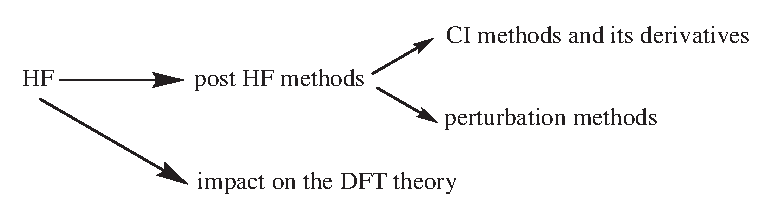
\includegraphics[scale=1.0]{HFpicture.eps}\label{HFT:2}
\caption{description of relationship between HF and other theories}
\end{center}
\end{figure}


%%%%%%%%%%%%%%%%%%%%%%%%%%%%%%%%%%%%%%%%%%%%%%%%%%%%%%%%
\section{Expression of Total Energy}
%
% 1  single electron approximation
% 2  expression of the whole wave function on the base of single electron approximation
% 3  one electron integral
% 4  two electron integral
% 5  the total energy
% 6  the total energy expression based on the basis sets
%
%
%
Here in this chapter, we are going to derive the Hatree-Fock theory.
The way we derive for this section and sections below in this
chapter is taken from some classic quantum chemistry  books
\cite{levine, szabo, pople, dewar}. And the best book to penetrate
into this area, the author recommends the book by Szabo and
Ostlund\cite{szabo}. Herein this section, we designate the $\varphi$
as the molecule orbital, and the $\phi$ as the atomic orbital or
basis sets; the $\Psi$ is used to express the Slater determinant, 
and finally the $\Phi$ is used to denote the wave function based 
on the Slater determinants. Usually the label of $a,b,c,\cdots i,j,k$ etc.
expresses the MO and the Greek letter $\mu, \nu$ etc. signal the AO.
In the following chapter, we will focus on this nomenclature.

The first approximation introduced into the HF theory is the single
electron approximation. For a arbitrary $\Psi$, we suggest that it
contains $n$ electrons; then the introduction of the single electron
approximation means that the $\Psi$ can be decomposed into many
pieces, each is resided by one electron (here we do not involve the
spin into consideration for simplicity); and more importantly, these
piece are not interact with each other. So the $\Psi$ can be written
as:
\begin{equation}\label{}
    \Psi =
    \varphi_{1}(1)\varphi_{2}(2)\varphi_{3}(3)\cdots\varphi_{n}(n)
\end{equation}
This expression is originally promoted by Hatree, which has a
deficiency that it does not incorporate the Pauli restriction to the
wave function. So here the wave function of $\Psi$ is just like the
wave systems we deal with in the classic mechanics. Here, the core
of the single electron approximation, is to simplify the total wave
function containing $n$ electrons into some pieces.

Later slater use the determinant to include the Pauli restriction to
the wave function, and rewrite the $\Psi$ as:
\begin{equation}\label{HFTeq:20}
\Psi = \frac{1}{\sqrt[2]{n!}} \left | \begin{array}{cccc}
  \varphi_{1}(1) & \varphi_{2}(1) & \cdots & \varphi_{n}(1) \\
  \varphi_{1}(2) & \varphi_{2}(2) & \cdots & \varphi_{n}(2) \\
  \cdots & \cdots & \cdots & \cdots                        \\
  \varphi_{1}(n) & \varphi_{2}(n) & \cdots & \varphi_{n}(n)
\end{array} \right |
\end{equation}
So interchanging the $\varphi$ or electron label will lead to the
$\Psi$ to alter its sign. When use the slater determinant form, it's
always appropriate to rewrite it into another equivalent form:
\begin{equation}\label{}
    \Psi = \frac{1}{\sqrt[2]{n!}} \sum_{p}(-1)^{p}P
    \{\varphi_{1}(1)\varphi_{2}(2)\varphi_{3}(3)\cdots\varphi_{n}(n)\}
\end{equation}
Herein this expression, the $P$ is the permutation of the electrons,
which makes electron i permutate over all orbitals. Since there must
be $n!$ terms in the slater determinant, so that we have to multiply
a normalizing factor of $\frac{1}{\sqrt[2]{n!}}$.

So far let's consider the decomposition of the schrodinger operator
of $\hat{H}$:
\begin{equation}\label{HFTeq:21}
    \hat{H}= \left\{\sum_{i=1}^{n}(\frac{-1}{2}\nabla_{i}^2)
    +\sum_{i=1}^{n}\sum_{\alpha=1}^{N}(\frac{-1}{r_{i\alpha}})
    +\sum_{i<j}(\frac{1}{r_{ij}})
\right\}
\end{equation}
It can be divided into two groups, one is the single electron
operator $\hat{H_{1}}$, and the other is the double electron
$\hat{H_{2}}$ operator. $\hat{H_{1}}$ embodies the kinetics and
electron-nuclear operator; and the $\hat{H_{2}}$ embodies the
electron repulsion operator. So let's concentrate on the energy of
each part.

For the $\hat{H_{1}}$, the energy can be expressed as:
\begin{multline}\label{HFTeq:4}
E_{1}=\frac{1}{n!}\langle\Psi|\hat{H_{1}}|\Psi\rangle \\
\shoveleft{=\frac{1}{n!}\sum_{p}\sum_{p^{'}} \langle (-1)^{p}P
\left \{ \varphi_{1}(1)\varphi_{2}(2)\varphi_{3}(3)\cdots\varphi_{n}(n)\right \} |}  \\
\hat{H_{1}}|(-1)^{p^{'}}P^{'} \left \{
\varphi_{1}(1)\varphi_{2}(2)\varphi_{3}(3)\cdots\varphi_{n}(n)\right
\} \rangle
\end{multline}
We can extend $\hat{H_{1}}$here to the form:
\begin{eqnarray}
% \nonumber to remove numbering (before each equation)
  \hat{H_{1}} &=&  \sum_{i=1}^{n}\hat{H}_{single} \nonumber \\
   &=& \sum_{i=1}^{n}\left\{(\frac{-1}{2}\times\nabla_{i}^2)+
   \sum_{\alpha=1}^{N}(\frac{-1}{r_{i\alpha}})\right\}
\end{eqnarray}
So $\hat{H}_{single}$ means the operator on the single electron who
has label of i.

By this way, the integrals of the system orbitals in the
(\ref{HFTeq:4}) can be expressed simply as:
\begin{eqnarray}\label{HFTeq:3}
% \nonumber to remove numbering (before each equation)
 \langle\Psi|\hat{H_{1}}|\Psi\rangle &=& \sum_{i=1}^{n}
\langle\Psi|\hat{H}_{single}|\Psi\rangle \nonumber \\
   &=& n\langle\Psi|\hat{H}_{single}|\Psi\rangle
\end{eqnarray}
For all the n electrons are undistinguished with each other.

So now we can safely assume that the $\hat{H}_{single}$ is the
$\hat{H}(1)$, which means that the operator is from the electron who
has the label of 1.

Moreover, let's interpret the permutation operator in much detailed
form. Since the $\Psi$ is a determinant, the $\Psi$ can be expressed
into the form below according to the Laplace theorem:
\begin{equation}\label{HFTeq:13}
\Psi = \sum^{n}_{i}\varphi_{i}(1)\Delta^{(i,1)}(2,3,4,\cdots,n)
\end{equation}
this expression has a very clear meaning. the $\Delta^{(i,1)}$
represents that the permutation operator is over all the orbitals
and electrons except orbital i and electron 1. this form is
equivalent to the form below:
\begin{equation}
\Psi = \sum^{n}_{i}\varphi_{i}(1) \times (-1)^{i+1} \left |
\begin{array}{cccccc}
  \varphi_{1}(2) & \cdots & \varphi_{i}(2) & \varphi_{i+1}(2) & \cdots & \varphi_{n}(2) \\
  \varphi_{1}(3) & \cdots & \varphi_{i}(3) & \varphi_{i+1}(3) & \cdots & \varphi_{n}(3) \\
  \cdots         & \cdots & \cdots         & \cdots           & \cdots & \cdots         \\
  \varphi_{1}(n) & \cdots & \varphi_{i}(n) & \varphi_{i+1}(n) & \cdots & \varphi_{n}(n)
\end{array}
\right |
\end{equation}
So with (\ref{HFTeq:13}) the (\ref{HFTeq:3}) can be further improved
as:
\begin{multline}\label{}
 \langle\Psi|\hat{H}_{1}|\Psi\rangle =n  \langle
\sum^{n}_{i}\varphi_{i}(1)\Delta^{(i,1)}(2,3,4,\cdots,n) |\\
\hat{H}(1)| \sum^{n}_{j}\varphi_{j}(1)\Delta^{(j,1)}(2,3,4,\cdots,n)
 \rangle
\end{multline}
and it yields:
\begin{multline}\label{HFTeq:14}
\langle\Psi|\hat{H}_{1}|\Psi\rangle = n \langle
\sum^{n}_{i}\varphi_{i}(1)|\hat{H}(1)|
\sum^{n}_{j}\varphi_{j}(1)  \rangle \\
\times \langle \Delta^{(i,1)}(2,3,4,\cdots,n)
|\Delta^{(j,1)}(2,3,4,\cdots,n)
 \rangle
\end{multline}
the $\langle \Delta^{(i,1)}(2,3,4,\cdots,n)
|\Delta^{(j,1)}(2,3,4,\cdots,n)
 \rangle$, is clearly to be $(n-1)!\delta_{ij}$. So with this consideration, it's easily
turned out that only $P=P^{'}$ leads to the
$\langle\Psi|\hat{H}_{1}|\Psi\rangle$ not equal to zero; which means
that the permutation between bra and ket should be same. Upon this
analysis, the (\ref{HFTeq:4}) can be:
\begin{eqnarray}
% \nonumber to remove numbering (before each equation)
  E_{1} &=& \frac{1}{n!}\times n! \langle
\sum^{n}_{i}\varphi_{i}(1)|\hat{H}(1)| \sum^{n}_{j}\varphi_{j}(1)
\rangle \nonumber  \\
   &=&
\sum^{n}_{i}\langle\varphi_{i}(1)|\hat{H}(1)|\varphi_{i}(1) \rangle
\end{eqnarray}
Since the $i$ and $j$ should vary consistently.

The derivation of the double electrons operator is similar to the
derivation for the single electron case above.
\begin{align}\label{}
\hat{H}_{2} &= \sum_{i<j}(\frac{1}{r_{ij}}) \nonumber \\
&=C^{2}_{n}(\frac{1}{r_{12}}) \nonumber \\
&=C^{2}_{n}\hat{H}_{double}
\end{align}
Here because electrons can not distinguish with each other,
therefore we can pick up the electron $1$ and $2$ to represent the
whole double electron operator.

then the energy expectation for the double electron operator is:
\begin{multline}\label{HFTeq:15}
  E_{2}=\frac{1}{n!}\langle\Psi|\hat{H}_{2}|\Psi\rangle \\
  \shoveleft{=\frac{1}{n!}C^{2}_{n}\sum_{p}\sum_{p^{'}}
  \langle
  (-1)^{p} \left \{\varphi_{1}(1)\varphi_{2}(2)\varphi_{3}(3)\cdots\varphi_{n}(n)\right\} |} \\
  \frac{1}{r_{12}}|
  (-1)^{p^{'}}P^{'}
           \left\{\varphi_{1}(1)\varphi_{2}(2)\varphi_{3}(3)\cdots\varphi_{n}(n)\right\}
\rangle
\end{multline}

Similarly, we can express the $\Psi$ as:
\begin{equation}\label{HFTeq:16}
\Psi = \sum^{n}_{i<j}\left|
                       \begin{array}{cc}
                         \varphi_{i}(1) & \varphi_{j}(1) \\
                         \varphi_{i}(2) & \varphi_{j}(2) \\
                       \end{array}
                     \right|
\Delta^{
            i,\,1 \choose
            j,\,2 }
(3,4,\cdots,n)
\end{equation}

By the same procedure used in $\hat{H}_{1}$, the (\ref{HFTeq:15})
can be transformed into the expression below while taking into the
account of (\ref{HFTeq:16}):
\begin{multline}\label{HFTeq:17}
 E_{2}=\frac{1}{n!}C^{2}_{n} \left
 \langle
\Delta^{
            i,\,1 \choose
            j,\,2 }
(3,4,\cdots,n) |
\Delta^{
            k,\,1 \choose
            l,\,2 }
(3,4,\cdots,n) \right\rangle  \\
\left\langle \sum^{n}_{i<j}
 \left|
 \begin{array}{cc}
 \varphi_{i}(1) & \varphi_{j}(1) \\
 \varphi_{i}(2) & \varphi_{j}(2) \\
 \end{array} \right|
 \left |\frac{1}{r_{12}} \right|
 \sum^{n}_{k<l}
  \left|
 \begin{array}{cc}
 \varphi_{k}(1) & \varphi_{l}(1) \\
 \varphi_{k}(2) & \varphi_{l}(2) \\
 \end{array}
 \right|
 \right\rangle
\end{multline}

So let's pay more attention to the (\ref{HFTeq:17}). The expression
below:
\begin{equation}\label{}
\left
 \langle
\Delta^{
            i,\,1 \choose
            j,\,2 }
(3,4,\cdots,n) | \Delta^{
            k,\,1 \choose
            l,\,2 }
(3,4,\cdots,n) \right\rangle
\end{equation}
equals to $(n-2)!\delta_{ik}\delta_{jl}$ (actually we have the
relation that $(i, j) = (k, l)$. However, since the relation that
$i< j$ and $k < l$, $i$ must equal to $k$ and $j$ must equal to $l$
). Thus the integral related to $\frac{1}{r_{12}}$ can be expanded as:
\begin{align}\label{HFTeq:22}
&\delta_{ik}\delta_{jl}\left\langle \sum^{n}_{i<j}
 \left|
 \begin{array}{cc}
 \varphi_{i}(1) & \varphi_{j}(1) \\
 \varphi_{i}(2) & \varphi_{j}(2) \\
 \end{array} \right|
 \left |\frac{1}{r_{12}} \right|
 \sum^{n}_{k<l}
  \left|
 \begin{array}{cc}
 \varphi_{k}(1) & \varphi_{l}(1) \\
 \varphi_{k}(2) & \varphi_{l}(2) \\
 \end{array}
 \right|
 \right\rangle \nonumber \\ 
&=\sum_{i<j}^{n} \left \{
2\langle\varphi_{i}(1)\varphi_{j}(2)|\frac{1}{r_{12}}|
\varphi_{i}(1)\varphi_{j}(2)\rangle -
2\langle\varphi_{i}(1)\varphi_{j}(2)|\frac{1}{r_{12}}|
\varphi_{i}(2)\varphi_{j}(1)\rangle
 \right \}
\end{align}
Since $2\sum_{i<j}$ equals to $\sum_{i}\sum_{j}$ (here we take
notice of the case where $i=j$. In this case (\ref{HFTeq:22}) equal
to $0$), so finally the (\ref{HFTeq:17}) is:
\begin{equation}\label{}
E_{2}=\frac{1}{2}\sum_{i,j}\left\{
\langle\varphi_{i}(1)\varphi_{j}(2)|\frac{1}{r_{12}}|\varphi_{i}(1)\varphi_{j}(2)\rangle-
\langle\varphi_{i}(1)\varphi_{j}(2)|\frac{1}{r_{12}}|\varphi_{j}(1)\varphi_{i}(2)\rangle
\right\}
\end{equation}

All in all,  the total energy is:
\begin{multline}\label{HFTeq:6}
% \nonumber to remove numbering (before each equation)
  E = E_{1}+E_{2}  \\
    \shoveleft{=\sum_{i}^{n}\langle\varphi_{i}(1)|\hat{H}(1)|\varphi_{i}(1)\rangle
    +}  \\
\frac{1}{2}\sum_{i}\sum_{j} \left\{
\langle\varphi_{i}(1)\varphi_{j}(2)|\frac{1}{r_{12}}|\varphi_{i}(1)\varphi_{j}(2)\rangle-
\langle\varphi_{i}(1)\varphi_{j}(2)|\frac{1}{r_{12}}|\varphi_{j}(1)\varphi_{i}(2)\rangle
\right\}
\end{multline}

%%%%%%%%%%%%%%%%%%%%%%%%%%%%%%%%%%%%%%%%%%%%%%%%%%%%%%
\section{General Notion}\label{General_Notion_Hatree-Fock}
%
%
%
%
So far the energy expression has been growing to be very
complicated, so it's appropriate to generalize some notations to
compact the one and two electron integrals.

For the one electron integral:
\begin{equation}\label{HFTeq:28}
\int \varphi^{*}_{i}(1)\hat{H}(1)\varphi_{j}(1) d\tau_{1}
\end{equation}
it's usually shorten as $\langle i|h|j \rangle$, or $[ i|h|j ]$,
$(i|h|j)$ (chemists always use this form), or even $h_{ij}$.

For the two electron integral:
\begin{equation}\label{HFTeq:29}
\int
\varphi^{*}_{i}(1)\varphi^{*}_{j}(2)\frac{1}{r_{12}}\varphi_{k}(1)\varphi_{l}(2)
d\tau_{1} d\tau_{2}
\end{equation}
We usually have two options:
\begin{itemize}
 \item the first option is that we specify it as $\langle ij|kl \rangle$, that
is to put the bra and ket separately. Physicists prefer this expression.
 \item the other option is to express it as $[ ik|jl ]$ or $(ik|jl)$, which we
put the electrons with same label together (ket is followed by bra). This is
favored by chemists.
\end{itemize}

So the (\ref{HFTeq:6}) can be:
\begin{equation}\label{HFTeq:24}
E = \sum^{n}_{i} \langle i|h|i \rangle +
\frac{1}{2}\sum^{n}_{i}\sum^{n}_{j} \{\langle ij|ij \rangle -\langle
ij|ji \rangle \}
\end{equation}
or in the chemical way:
\begin{equation}\label{HFTeq:24-1}
E = \sum^{n}_{i} ( i|h|i ) +
\frac{1}{2}\sum^{n}_{i}\sum^{n}_{j} \{( ii|jj ) -(
ij|ji ) \}
\end{equation}

Usually the differential form of Hatree-Fock equation is difficult
to solve, so that we use the basis sets to expand the molecular
orbitals:
\begin{equation}\label{HFTeq:8}
    \varphi_{i} = \sum_{\mu}c_{\mu i}\phi_{\mu}
\end{equation}
Here the Greek letter indicates the use of the atomic orbitals (AO). By
inserting the expression of $\varphi$ into the
(\ref{HFTeq:6}), we can get:
\begin{multline}\label{HFTeq:7}
E = \sum_{i}\sum_{\mu} \sum_{\nu} C^{*}_{\mu i} C_{\nu
i} \langle\phi_{\mu}(1)|\hat{H}(1)|\phi_{\nu}(1)\rangle +  \\
\frac{1}{2} \sum_{i}\sum_{j}\sum_{\mu} \sum_{\nu} \sum_{\lambda}
\sum_{\sigma} C^{*}_{\mu i} C_{\nu i} C^{*}_{\lambda j} C_{\sigma j}
\\
 \left\{
\langle\phi_{\mu}(1)\phi_{\lambda}(2)|\hat{H}(12)|\phi_{\nu}(1)\phi_{\sigma}(2)\rangle-
\langle\phi_{\mu}(1)\phi_{\lambda}(2)|\hat{H}(12)|\phi_{\sigma}(1)\phi_{\nu}(2)\rangle
\right \}
\end{multline}
Here according to the notation we have discussed, we can make some
abbreviations to the (\ref{HFTeq:7}), to make it looks more clear.
First, we can abbreviate the single electron integral as:
\begin{equation}\label{}
\langle\phi_{\mu}|\hat{H}(1)|\phi_{\nu}\rangle = h_{\mu \nu}
\end{equation}
Then the double electron integral can be written as:
\begin{equation}\label{}
% \nonumber to remove numbering (before each equation)
  \langle\phi_{\mu}(1)\phi_{\lambda}(2)|\hat{H}(12)|\phi_{\nu}(1)\phi_{\sigma}(2)\rangle
  = \langle \mu\lambda | \nu\sigma \rangle
\end{equation}
Furthermore, we can define the ``density matrix'' as
$\sum_{i}C^{*}_{\mu i} C_{\nu i} = P_{\mu\nu}$. whose meaning
will be further discussed in the following content.

On the base of the discussion above, we have (\ref{HFTeq:7}) shorten
as:
\begin{equation}\label{HFTeq:11}
    E = \sum_{\mu \nu}P_{\mu\nu}h_{\mu \nu} + \frac{1}{2}
    \sum_{\mu \nu \lambda\sigma}P_{\mu\nu}P_{\lambda\sigma}
    \left \{ \langle\mu\lambda | \nu\sigma\rangle - \langle\mu \lambda | \sigma\nu\rangle
    \right \}
\end{equation}
Or the form that:
\begin{equation}\label{HFTeq:11-1}
    E = \sum_{\mu \nu}P_{\mu\nu}h_{\mu \nu} + \frac{1}{2}
    \sum_{\mu \nu \lambda\sigma}P_{\mu\nu}P_{\lambda\sigma}
    \left \{ (\mu\nu|\lambda\sigma) - (\mu \sigma|\lambda\nu)
    \right \}
\end{equation}

%%%%%%%%%%%%%%%%%%%%%%%%%%%%%%%%%%%%%%%%%%%%%%%%%%%

\section{Physical Meaning of Total Energy}\label{PMTE_for_HF}
% the most important concept is orbitals are independent with each other,
% so there's no cross terms in the energy expression
% one electron integral: no cross terms
% coulomb energy, how to count
% exchange energy, how to count; the origin is from determinant
% on the basis sets, how to understand the density
% how to understand the density matrix
%
Here we can see what's the meaning of the total energy. And now
let's interpret it in a more pictorial way.

The essence of HF theory, is to approximate the wave function as
slater determinant. Since the orbitals are not interact with each
other, it can be well expected that there's no cross term in the
energy expression; and the derivation above indeed demonstrates this
point.

The one electron integral, is divided into two parts: the electron
kinetic energy and nuclear electron attraction energy. From the last
section it can see that their expectation values are summing over
all orbitals, and no cross term in the final result.

As for the double electron integral, it can be partitioned into two
parts: the coulomb energy and the exchange energy. Before we step
into the physical interpretation of both of the two terms, let's
shift to the real picture of the interaction between two electrons.

Suppose that we have electron 1 at place $\tau_{1}$ and electron 2
at place $\tau_{2}$, if there's little change in the motion of
electron 2 will cause instantaneous motion change in electron 1.
This is coincident with the uncertainty law: in quantum mechanical
world, the motion of any two electrons can never be independent with
each other since that their wave functions can be always superposed
together so that the interaction happens.

However, in Hatree-Fock picture the electrons are assumed to be
independent with each other, thus there must be some part of effects
which fail to conclude into the energy expression, this part is
called correlation energy.

Then let's go to see the coulomb energy. First we can specify the
term in (\ref{HFTeq:6}) as:
\begin{equation}\label{}
\frac{1}{2}\sum_{i}\sum_{j} \int
\varphi^{*}_{i}(1)\varphi_{i}(1)
\frac{1}{r_{12}}\varphi^{*}_{j}(2)\varphi_{j}(2)
d\tau_{1} d\tau_{2}
\end{equation}

Here the $|\varphi_{i}(1)|^{2}d\tau_{1}$ represents the
infinitesimal density of electron 1 at position of $d\tau_{1}$, so
as the $|\varphi_{j}(2)|^{2}d\tau_{2}$; and the integral under
operation of $\frac{1}{r_{12}}$ denotes the coulomb energy between
electron 1 at position of $d\tau_{1}$ and electron 2 at position of
$d\tau_{2}$. By summing up all the $j$ orbitals as well as summing
up over all the $i$ orbitals, we can get the average coulomb
potential felt by the electron density at position 1 and position 2. Finally
since we count each one orbital twice, we times a factor of $1/2$. Hence we can
actually express it into much more clear form:
\begin{align}\label{HF_PMTE_eq:1}
&\frac{1}{2}\sum_{i}\sum_{j} \int
\varphi^{*}_{i}(1)\varphi_{i}(1)
\frac{1}{r_{12}}\varphi^{*}_{j}(2)\varphi_{j}(2)
d\tau_{1} d\tau_{2} \nonumber \\
&= \frac{1}{2} \int \rho(r)
\frac{1}{|r-r^{'}|}\rho(r^{'})
d r dr^{'}
\end{align}

In the coulomb energy expression, it's interesting to see that it's
irrelevant to the spin consideration. therefore, if we assume
there's one electron on the molecular orbital, then we use the
result above; if two electrons occupied on the orbital, then we
multiply a factor of $2$ since both of the two electrons make same
contributions.

The exchange term from the (\ref{HFTeq:6}) is arising from the
antisymmetric nature of the single determinant, and it has a
somewhat strange form and does not have a simple classic
interpretation like coulomb term:
\begin{equation}\label{}
-\frac{1}{2}\sum_{i}\sum_{j} \int \varphi^{*}_{i}(1)\varphi_{j}(1)
\frac{1}{r_{12}}\varphi^{*}_{j}(2)\varphi_{i}(2) d\tau_{1} d\tau_{2}
\end{equation}

However, we can still use some simple notion to express it:
\begin{align}\label{HF_PMTE_eq:2}
& -\frac{1}{2}\sum_{i}\sum_{j} \int \varphi^{*}_{i}(1)\varphi_{j}(1)
\frac{1}{r_{12}}\varphi^{*}_{j}(2)\varphi_{i}(2) d\tau_{1} d\tau_{2} \nonumber
\\
& =  -\frac{1}{2}\sum_{i}\sum_{j} \int \varphi^{*}_{i}(1)\varphi_{i}(2)
\frac{1}{r_{12}}\varphi^{*}_{j}(2)\varphi_{j}(1) d\tau_{1}
d\tau_{2} \rightarrow \nonumber \\
&= -\frac{1}{2}\int \rho(r1, r2)\frac{1}{r_{12}}\rho(r2, r1)d\tau_{1}
d\tau_{2} \rightarrow \nonumber \\
&=  -\frac{1}{2}\int \rho(r, r^{'})\frac{1}{|r-r^{'}|}\rho(r^{'}, r)dr
dr^{'}
\end{align}
Here we introduce the exchange density $\rho(r1, r2) =
\sum_{i}\varphi^{*}_{i}(1)\varphi_{i}(2)$. Physically, this new density relies
on two position index (so it reflects the non-local property of the exchange
energy). In fact, in the following chapter discussing the reduced density
matrix, we can see that this is just the one dimensional reduced density matrix.

Now let's consider spin. It's obvious that $\rho_{\sigma\sigma^{'}}(r, r^{'}) =
0$ if $\sigma \neq \sigma^{'}$. Actually in the density matrix part, we can
show that:
\begin{equation}
 \int \rho_{\sigma\sigma^{'}}(r, r^{'}) dr^{'} = -\delta_{\sigma\sigma^{'}}
\end{equation}
This is called ``Fermi Hole'' for the exchange effects.

Finally let's go to see the density:
\begin{align}\label{HF_PMTE_eq:3}
 \rho(r) &= \sum_{i}|\varphi_{i}(r)|^{2} \nonumber \\
&= \sum_{i}\sum_{\mu}\sum_{\nu}c^{*}_{\mu i}c_{\nu i}\phi^{*}_{\mu}\phi_{\nu}
\nonumber \\
&= \sum_{\mu}\sum_{\nu}P_{\mu\nu}\phi^{*}_{\mu}\phi_{\nu}
\end{align}
It can be further partitioned by two parts:
\begin{align}\label{HF_PMTE_eq:4}
&\sum_{\mu}\sum_{\nu}P_{\mu\nu}\phi^{*}_{\mu}\phi_{\nu} \nonumber \\
&= \sum_{\mu}P_{\mu\nu}|\phi_{\mu}|^{2} + 
2\sum_{\mu<\nu}P_{\mu\nu}\phi^{*}_{\mu}\phi_{\nu}
\end{align}

Here in this expression, the $\sum_{\mu}P_{\mu\nu}|\phi_{\mu}|^{2}$ express the
electron density coming from the $\mu$th atom; and the other part where $\mu
< \nu$ describe the overlap of the orbitals which is coming from
different atoms, that makes up another part of the electron density.
Therefore by translating the abstract molecule orbital into the
concrete basis sets, we can have a more pictorial way to look into
the HF theory.

For the density matrix, who has the form of $\sum_{i}C^{*}_{\mu i}
C_{\nu i} = P_{\mu\nu}$; that is the summation of electron
density of all molecule orbitals, and between $\mu$th atom and
$\nu$th atom. if $\mu=\nu$, that indicates the pure electron distribution
of the atom $\mu$; if $\mu \neq \nu$, this indicates the electron
distribution within the area between atom $\mu$ and $\nu$, which can
be related to the chemical bond between atom $\mu$ and $\nu$.  In the following
section, we will move back to it again.


%%%%%%%%%%%%%%%%%%%%%%%%%%%%%%%%%%%%%%%
\section{Restricted and Unrestricted Cases}\label{RUC_in_HF}
%
%
There are generally two ways to form the Slater determinants: one is
the restricted type and the other is the unrestricted type. In the restricted
type (RHF or ROHF), the electrons in the molecule are grouped into pairs to
reside on the molecular orbitals starting from the lowest energy one; while in
the other case (UHF) the electrons in different spin states are assumed to
independently occupy the orbitals, that means their spatial part is also
different (see \ref{HFTpic:4}). 

\begin{figure}[htbp]
\begin{center}
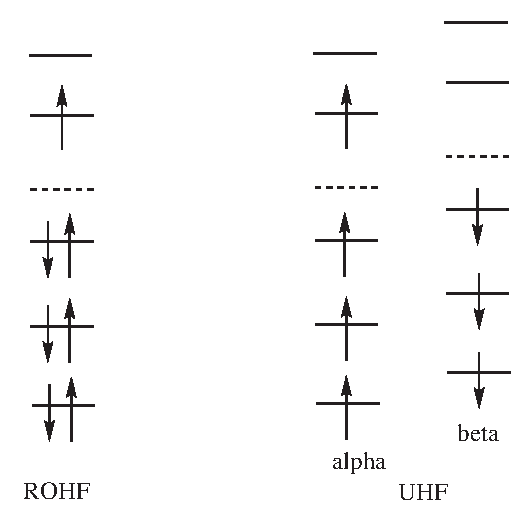
\includegraphics[scale=0.7]{uhfrohf.eps}
\caption{UHF and ROHF description}
\label{HFTpic:4}
\end{center}
\end{figure}

Let's start from our last section conclusion, that to express the terms into
density and exchange density form. For the one electron integral, actually the
spin will not affect its form. For the coulomb part, it's irrelevant to the
density, and for the exchange density, the spin cross term is zero. Hence let's
consider:
\begin{align}\label{}
r(\alpha) \quad &  r^{'}(\alpha) \nonumber \\
r(\alpha) \quad &  r^{'}(\beta) \nonumber \\
r(\beta) \quad &  r^{'}(\alpha) \nonumber \\
r(\beta) \quad &  r^{'}(\beta) \nonumber \\
\end{align}
For the coulomb term, all of four terms exist; and for exchange energy, the
second and third term vanish. Hence we can express the total energy generally
as:
\begin{equation}
  E = h_{\mu\nu}^{\alpha} + h_{\mu\nu}^{\beta} 
   + \frac{1}{2}\left[ C_{\alpha\alpha} + 
C_{\alpha\beta} + C_{\beta\alpha} + C_{\beta\beta}\right] -
\frac{1}{2}\left[ X_{\alpha\alpha} + X_{\beta\beta} \right] 
\end{equation}
Here $C_{\alpha\alpha}$ etc. is the terms expressed in (\ref{HF_PMTE_eq:1}) by
adding the spin consideration, and $X_{\alpha\alpha}$ is the exchange term in 
(\ref{HF_PMTE_eq:2}).

For the RHF case, we can get:
\begin{equation}\label{HFTeq:23}
  E = 2h_{\mu\nu} 
   + \left[ 2C_{r, r^{'}}  -  X_{r, r^{'}}  \right] 
\end{equation}
Since we need not to specify spin state anymore, so we just specify the
position vector.

For the UHF case
\begin{equation}\label{HFTeq:27}
  E = h_{\mu\nu}^{\alpha} + h_{\mu\nu}^{\beta}  
   + \frac{1}{2}\left[ C_{\alpha\alpha} + 
C_{\alpha\beta} + C_{\beta\alpha} + C_{\beta\beta}\right] -
\frac{1}{2}\left[ X_{\alpha\alpha} + X_{\beta\beta} \right] 
\end{equation}
Since alpha part and beta usually not equal to each other anymore.


%%%%%%%%%%%%%%%%%%%%%%%%%%%%%%%%%%%%%%%%%%%%
\section{The Derivation of The Hatree-Fock Equation}
\subsection{Variation Process}\label{HFT:6}
% 1  physical meaning of the variation process: through the variation
%     of total energy we get the HF function
% 2  meaning of HF function
%
%
%
From the discussion above, we can see that under single electron
approximation; the total energy has been expressed as the functional
of orbitals. So eventually, the total energy is the functional of
the molecule orbital space. Under the constraint of maintaining
perpendicular condition (this is required by the single electron
approximation), as the molecule orbitals continuously make an
infinitesimal change, the total energy is also coincidentally
changed. Our target, is to find the expression as $\frac{\delta
E}{\delta \Psi} = 0$. That's the stationary point of the
$E=F[\Psi]$\footnote{Personally I hate this long derivation. However, it's
detailed and rigorous. On the other hand, we need a point of view that to
understand the HF theory from the MO variation}.

The perpendicular condition required in the variation process is:
\begin{align}\label{}
    \int\delta\varphi_{i}\varphi_{j}d\tau &= \delta_{ij} \nonumber \\
    \int\varphi_{i}\delta\varphi_{j}d\tau &= \delta_{ij}
\end{align}
It's worthy to note that in the variational process, we care about the first
order varied $\Psi$ so all the second order terms, like
$\delta\varphi_{i}\delta\varphi_{j}$ are all ignored.

Now we enter the variation process. Under such constraint, it's
necessarily to use the lagrange variation process. Firstly, let's go
into the variation process based on the molecule orbitals.

As molecule orbital
$\varphi_{i}\rightarrow\varphi_{i}+\delta\varphi_{i}$, the energy is
also changed $E\rightarrow E+\delta E$. We vary the expression
below(the general total energy expression is concerned):
\begin{multline}\label{HFTeq:1}
% \nonumber to remove numbering (before each equation)
  G =\sum_{i}^{n}\langle\varphi_{i}(1)|\hat{H}(1)|\varphi_{i}(1)\rangle
    +  \\
\frac{1}{2}\sum_{i}\sum_{j} \left\{
\langle\varphi_{i}(1)\varphi_{j}(2)|\frac{1}{r_{12}}|\varphi_{i}(1)\varphi_{j}(2)\rangle-
\langle\varphi_{i}(1)\varphi_{j}(2)|\frac{1}{r_{12}}|\varphi_{j}(1)\varphi_{i}(2)\rangle
\right\} \\
-(\sum_{i}\sum_{j}\varepsilon_{ij}\langle\varphi_{i}(1)|\varphi_{j}(1)\rangle
-\delta_{ij} )
\end{multline}
The last term introduce the orthogonality restriction in the MO variation
process.

Obviously the G is different from E only by a constant added by the
final term. Here $\varepsilon_{ij}$ is purely some Lagrangian
factor.

Therefore, $\delta G$ gets to:
\begin{multline}\label{HFTeq:2}
\delta G = \sum_{i}^{n} \left \{
\langle\delta\varphi_{i}(1)|\hat{H}(1)|\varphi_{i}(1)\rangle +
\langle\varphi_{i}(1)|\hat{H}(1)|\delta\varphi_{i}(1)\rangle
\right\} +  \\
\frac{1}{2}\sum_{i}\sum_{j} \left\{
\langle\delta\varphi_{i}(1)\varphi_{j}(2)|\frac{1}{r_{12}}|\varphi_{i}(1)\varphi_{j}(2)\rangle
+
\langle\varphi_{i}(1)\delta\varphi_{j}(2)|\frac{1}{r_{12}}|\varphi_{i}(1)\varphi_{j}(2)\rangle
\right\} +  \\
\frac{1}{2}\sum_{i}\sum_{j} \left\{
\langle\varphi_{i}(1)\varphi_{j}(2)|\frac{1}{r_{12}}|\delta\varphi_{i}(1)\varphi_{j}(2)\rangle
+
\langle\varphi_{i}(1)\varphi_{j}(2)|\frac{1}{r_{12}}|\varphi_{i}(1)\delta\varphi_{j}(2)\rangle
\right\} - \\
\frac{1}{2}\sum_{i}\sum_{j} \left\{
\langle\delta\varphi_{i}(1)\varphi_{j}(2)|\frac{1}{r_{12}}|\varphi_{j}(1)\varphi_{i}(2)\rangle
+
\langle\varphi_{i}(1)\delta\varphi_{j}(2)|\frac{1}{r_{12}}|\varphi_{j}(1)\varphi_{i}(2)\rangle
\right\} - \\
\frac{1}{2}\sum_{i}\sum_{j} \left\{
\langle\varphi_{i}(1)\varphi_{j}(2)|\frac{1}{r_{12}}|\delta\varphi_{j}(1)\varphi_{i}(2)\rangle
+
\langle\varphi_{i}(1)\varphi_{j}(2)|\frac{1}{r_{12}}|\varphi_{j}(1)\delta\varphi_{i}(2)\rangle
\right\} \\
- \sum_{i}\sum_{j} \varepsilon_{ij}\left\{
\langle\delta\varphi_{i}(1)|\varphi_{j}(1)\rangle +
\langle\varphi_{i}(1)|\delta\varphi_{j}(1)\rangle
 \right\}
\end{multline}

Now first we have to make some implications for the (\ref{HFTeq:2}).
There's two general rules for us; since that the operator of
$1/r_{12}$ is some hermite operator then we can safely exchange the
bra and ket, that's the first transformation; secondly, because the
electrons are undistinguished with each other thus we can exchange
the electron label in the integrals without changing it.

For the coulomb integrals, let's use the first rule to exchange the
bra and ket; then we can find:
\begin{align}\label{}
\langle\delta\varphi_{i}(1)\varphi_{j}(2)|\frac{1}{r_{12}}|
\varphi_{i}(1)\varphi_{j}(2)\rangle &=
\langle\varphi_{i}(1)\varphi_{j}(2)|\frac{1}{r_{12}}|
\delta\varphi_{i}(1)\varphi_{j}(2)\rangle \nonumber \\
\langle\varphi_{i}(1)\delta\varphi_{j}(2)|\frac{1}{r_{12}}|
\varphi_{i}(1)\varphi_{j}(2)\rangle &=
\langle\varphi_{i}(1)\varphi_{j}(2)|\frac{1}{r_{12}}|
\varphi_{i}(1)\delta\varphi_{j}(2)\rangle
\end{align}

For the exchange integrals, firstly we exchange the electron label
then then do the same thing for the bra and ket; finally we can get:
\begin{align}\label{}
\langle\delta\varphi_{i}(1)\varphi_{j}(2)|\frac{1}{r_{12}}|
\varphi_{j}(1)\varphi_{i}(2)\rangle &=
\langle\varphi_{i}(1)\varphi_{j}(2)|\frac{1}{r_{12}}|
\varphi_{j}(1)\delta\varphi_{i}(2)\rangle \nonumber \\
\langle\varphi_{i}(1)\delta\varphi_{j}(2)|\frac{1}{r_{12}}|
\varphi_{j}(1)\varphi_{i}(2)\rangle &=
\langle\varphi_{i}(1)\varphi_{j}(2)|\frac{1}{r_{12}}|
\delta\varphi_{j}(1)\varphi_{i}(2)\rangle
\end{align}

Finally, by gathering all the results above, we can transform the
(\ref{HFTeq:2}) into:
\begin{multline}\label{}
\delta G = \sum_{i}^{n} \left \{
\langle\delta\varphi_{i}(1)|\hat{H}(1)|\varphi_{i}(1)\rangle +
\langle\varphi_{i}(1)|\hat{H}(1)|\delta\varphi_{i}(1)\rangle
\right\} +  \\
\sum_{i}\sum_{j} \left\{
\langle\delta\varphi_{i}(1)\varphi_{j}(2)|\frac{1}{r_{12}}|\varphi_{i}(1)\varphi_{j}(2)\rangle
+
\langle\varphi_{i}(1)\varphi_{j}(2)|\frac{1}{r_{12}}|\varphi_{i}(1)\delta\varphi_{j}(2)\rangle
\right\} - \\
\sum_{i}\sum_{j} \left\{
\langle\delta\varphi_{i}(1)\varphi_{j}(2)|\frac{1}{r_{12}}|\varphi_{j}(1)\varphi_{i}(2)\rangle
+
\langle\varphi_{i}(1)\varphi_{j}(2)|\frac{1}{r_{12}}|\delta\varphi_{j}(1)\varphi_{i}(2)\rangle
\right\} \\
- \sum_{i}\sum_{j} \varepsilon_{ij}\left\{
\langle\delta\varphi_{i}(1)|\varphi_{j}(1)\rangle +
\langle\varphi_{i}(1)|\delta\varphi_{j}(1)\rangle
 \right\}
\end{multline}
Here for the two electron integrals, we drive all the
$\delta\varphi_{i}$ into the bra, and $\delta\varphi_{j}$ into the
ket.

Furthermore, the above expression can be classified into two groups;
that is:
\begin{equation}\label{HFTeq:33}
\begin{split}
\delta G  &=
\Bigg\{ \sum_{i}^{n}
\langle\delta\varphi_{i}(1)|\hat{H}(1)|\varphi_{i}(1)\rangle
 +
\sum_{i}\sum_{j} \left(
\langle\delta\varphi_{i}(1)\varphi_{j}(2)|\frac{1}{r_{12}}|
\varphi_{i}(1)\varphi_{j}(2)\rangle - \right. \\
&\left.\langle\delta\varphi_{i}(1)\varphi_{j}(2)|\frac{1}{r_{12}}|
\varphi_{j}(1)\varphi_{i}(2)\rangle \right) - \sum_{i}\sum_{j}
\varepsilon_{ij}
\langle\delta\varphi_{i}(1)|\varphi_{j}(1)\rangle \Bigg\} + \\
&\Bigg\{ \sum_{i}^{n}
\langle\varphi_{i}(1)|\hat{H}(1)|\delta\varphi_{i}(1)\rangle
 +
\sum_{i}\sum_{j} \left(
\langle\varphi_{i}(1)\varphi_{j}(2)|\frac{1}{r_{12}}|
\varphi_{i}(1)\delta\varphi_{j}(2)\rangle - \right. \\
&\left.\langle\varphi_{i}(1)\varphi_{j}(2)|\frac{1}{r_{12}}|
\delta\varphi_{j}(1)\varphi_{i}(2)\rangle \right) - \sum_{i}\sum_{j}
\varepsilon_{ij}
\langle\varphi_{i}(1)|\delta\varphi_{j}(1)\rangle\Bigg\}
\end{split}
\end{equation}

Continuously, we can exchange the label of electrons to further
simplify the (\ref{HFTeq:33}). Firstly we have:
\begin{equation}\label{}
\begin{split}
& \langle\varphi_{i}(1)\varphi_{j}(2)|\frac{1}{r_{12}}|
\varphi_{i}(1)\delta\varphi_{j}(2)\rangle -
\langle\varphi_{i}(1)\varphi_{j}(2)|\frac{1}{r_{12}}|
\delta\varphi_{j}(1)\varphi_{i}(2)\rangle \\
&= \langle\varphi_{i}(1)\varphi_{j}(2)|\frac{1}{r_{12}}|
\varphi_{i}(1)\delta\varphi_{j}(2)\rangle -
\langle\varphi_{i}(2)\varphi_{j}(1)|\frac{1}{r_{12}}|
\delta\varphi_{j}(2)\varphi_{i}(1)\rangle
\end{split}
\end{equation}

Then by bringing the above result into the (\ref{HFTeq:33}), we can
have:
\begin{equation}\label{HFTeq:34}
\begin{split}
\delta G  &= \Bigg\{ \sum_{i}^{n}
\langle\delta\varphi_{i}(1)|\hat{H}(1)|\varphi_{i}(1)\rangle
 +
\sum_{i}\sum_{j} \left(
\langle\delta\varphi_{i}(1)\varphi_{j}(2)|\frac{1}{r_{12}}|
\varphi_{i}(1)\varphi_{j}(2)\rangle - \right. \\
&\left.\langle\delta\varphi_{i}(1)\varphi_{j}(2)|\frac{1}{r_{12}}|
\varphi_{j}(1)\varphi_{i}(2)\rangle \right) - \sum_{i}\sum_{j}
\varepsilon_{ij}
\langle\delta\varphi_{i}(1)|\varphi_{j}(1)\rangle \Bigg\} + \\
&\Bigg\{ \sum_{j}^{n}
\langle\varphi_{j}(2)|\hat{H}(2)|\delta\varphi_{j}(2)\rangle
 +
\sum_{i}\sum_{j} \left(
\langle\varphi_{i}(1)\varphi_{j}(2)|\frac{1}{r_{12}}|
\varphi_{i}(1)\delta\varphi_{j}(2)\rangle - \right. \\
&\left.\langle\varphi_{j}(1)\varphi_{i}(2)|\frac{1}{r_{12}}|
\varphi_{i}(1)\delta\varphi_{j}(2)\rangle \right) - \sum_{i}\sum_{j}
\varepsilon_{ij}
\langle\varphi_{i}(2)|\delta\varphi_{j}(2)\rangle\Bigg\}
\end{split}
\end{equation}

Now thing becomes clear. In the (\ref{HFTeq:34}) we note that the
$\langle\delta\varphi_{i}|$ and $|\delta\varphi_{j}\rangle$ vary
independently, thus we can write the (\ref{HFTeq:34}) generally as:
\begin{multline}\label{HFTeq:5}
\delta G = \sum_{i}^{n}
\langle\delta\varphi_{i}(1)|\hat{H}(1)|\varphi_{i}(1)\rangle \\
+ \sum_{i}\sum_{j} \left\{
\langle\delta\varphi_{i}(1)\varphi_{j}(2)|\frac{1}{r_{12}}|\varphi_{i}(1)\varphi_{j}(2)\rangle
-
\langle\delta\varphi_{i}(1)\varphi_{j}(2)|\frac{1}{r_{12}}|\varphi_{j}(1)\varphi_{i}(2)\rangle
\right\} \\
- \sum_{i}\sum_{j} \varepsilon_{ij}
\langle\delta\varphi_{i}(1)|\varphi_{j}(1)\rangle + \text {other
terms}
\end{multline}

Therefore as $\delta G = 0$ then the two independent
$\langle\delta\varphi_{i}|$ and $|\delta\varphi_{j}\rangle$ will
become zero separately, that means each sum will go zero in the
independent way in the (\ref{HFTeq:34}). Then in the (\ref{HFTeq:5})
we can lift the $\sum_{i}^{n}\langle\delta\varphi_{i}(1)|$ outside,
it gives:
\begin{multline}\label{HFTeq:9}
\hat{H}(1)\varphi_{i}(1) + \sum_{j}^{occ}\left[
\left\{\int\varphi^{*}_{j}(2)\varphi_{j}(2)d\tau(2)\frac{1}{r_{12}}\right\}\varphi_{i}(1)
\right] \\
 -
\sum_{j}^{occ}\left[
\left\{\int\varphi^{*}_{j}(2)\varphi_{i}(2)d\tau(2)\frac{1}{r_{12}}\right\}\varphi_{j}(1)
\right] \\
 = \sum_{j} \varepsilon_{ij}\varphi_{j}(1)
\end{multline}
This is the most famous Hatree-Fock Equation.

If we define two new operator related to the coulomb and exchange
term, we can have:
\begin{eqnarray}\label{HFTeq:31}
% \nonumber to remove numbering (before each equation)
  J_{i} &=& \int\varphi^{*}_{j}(2)\varphi_{j}(2)d\tau(2)\frac{1}{r_{12}} \nonumber \\
  K_{i} &=& \left[\int\varphi^{*}_{j}(2)\varphi_{i}(2)d\tau(2)\frac{1}{r_{12}}\right]\varphi_{j}(1)
\end{eqnarray}

The $K_{i}$ is an non-local operator, that means it not only depends
on the orbital j, also its formation depends on the orbital i it act
on. This operator, is the result of Pauli effects.

So finally the Hatree-Fock Equation is:
\begin{equation}\label{HFTeq:10}
\left\{\hat{H}(1)+ \sum_{j}[J_{i} - K_{i}] \right\}\varphi_{i} =
\sum_{j} \varepsilon_{ij}\varphi_{j}
\end{equation}
Or in short, we can define the Fock operator as:
\begin{equation}\label{}
\hat{F}(i) =\hat{H}(1)+ \sum_{i}[J_{i} - K_{i}]
\end{equation}
So the Hatree-Fock equation is:
\begin{equation}\label{}
\hat{F}(i)\varphi_{i} = \sum_{j} \varepsilon_{ij}\varphi_{j}
\end{equation}

We finally note that here all the orbitals related are the so called ``occupied
orbitals''. These orbitals have electrons residing on, so that they are
contributing to the electron density; and they are composed into the HF wave
functions (the Slater determinant indicated in \ref{HFTeq:20}); in turn to
form the total energy under the single electron approximation (result in
\ref{HFTeq:6}).

Here we make such clarification is that later we can show that as opposed to
the occupied orbitals, there are ``virtual orbitals''. By looking the equation
of \ref{HFTeq:10}), similar to the Schrodinger equation the Hatree-Fock
equation is also some eigen function so that it's able to produce
unlimited number of eigen states. The first $n$ lowest energy orbitals are the
occupied orbitals, there are just the molecular orbitals used in constructing
the Slater determinants in the (\ref{HFTeq:20}). The other molecular orbitals
left, is the so called ``virtual orbitals''.

However, as what we can see; so far the virtual orbitals are still not so
clear; since we can not write down some Lagrangian that contains the virtual
orbitals so to make variation to derive the Hatree-Fock equation for virtual
orbitals. The physical quantity, just like density, energy are all based on the
occupied orbitals so the exact equation for virtual orbital are not clear.
However, after the basis set functions are introduced, we will come back to
this point again.

All in all, we can see that the Hatree-Fock equation is different
with Schroedinger equation only by the single electron approximation.
Hence, the Hatree-Fock equation can be viewed as the some ``single
electron Schroedinger equation''.

%%%%%%%%%%%%%%%%%%%%%%%%%%%%%%%%%%%%%%%%%%%%%%%%%%
\subsection{Self-Consistent Field Methods}
%
%
%


Formally the Hatree-Fock equation derived in the (\ref{HFTeq:9}) is
a series of differential equations. Moreover, in such differential
equations the coulomb operator and the exchange operator also
depends on result molecular orbitals; Therefore, to solve such
equations people introduced the so called ``self-consistent field''
methods.

The self-consistent field method is working like this: first, we get
a group of trial functions of $\varphi_{1}, \varphi_{2}, \cdots$ so
that we can calculate the coulomb operator and the exchange
operator; then we can get a new sets of $\varphi^{'}_{1},
\varphi^{'}_{2}, \cdots$. If the new sets are same with the old ones
within the error range, then we get the final answer; else we will
use the new sets of molecular orbitals to recalculate the Fock
operator then repeat the above process until we get the
``consistent'' answer.


%%%%%%%%%%%%%%%%%%%%%%%%%%%%%%%%%%%%%%%%%%%%%%%
\subsection{Unitary Transformation}\label{HFT:3}
%
% how to understand the unitary transformation
%
%
At first glance, this result looks a bit of surprising. The Fock
operator done on the single molecule orbital $\varphi_{i}$, yet
leads to the result that has something to do with all the orbitals. However, we
can use some unitary operator  to transform the left side of (\ref{HFTeq:9})
into single orbitals.

Suggest we change the molecular orbitals into some new sets:
\begin{equation}\label{HFTeq:30}
\varphi_{i}^{'} = \sum_{k}T_{ki}\varphi_{k}
\end{equation}
Then, how to ensure that the new sets is equivalent to the 
original space? From the quantum mechanics, we can know that it
requires the transformation matrix of $T$ is unitary: $T^{+}T = I$;
this can be derived from the orthogonal relation:
\begin{align}\label{HFTeq:32}
\int\varphi_{i}^{'}\varphi_{j}^{'}d\tau &= \delta_{ij} \nonumber \\
\sum_{k}\sum_{l}T^{*}_{ki}T_{lj}\int\varphi^{*}_{k}\varphi_{l}d\tau
&= \delta_{ij} \nonumber \\
\sum_{k}\sum_{l}T^{*}_{ki}T_{lj}\delta_{kl}
&= \delta_{ij} \nonumber \\
\sum_{k}T^{*}_{ki}T_{kj}
&= \delta_{ij} \Rightarrow \nonumber \\
T^{+}T &= I
\end{align}

Now let's further investigate the unitary transformation of the
molecular orbitals. Firstly, we can prove that for the total HF wave
function of $\Psi$, the unitary transformation does not change it:
\begin{equation}\label{}
\Psi = \frac{1}{\sqrt[2]{n!}} \left | \begin{array}{cccc}
  \varphi_{1}(1) & \varphi_{2}(1) & \cdots & \varphi_{n}(1) \\
  \varphi_{1}(2) & \varphi_{2}(2) & \cdots & \varphi_{n}(2) \\
  \cdots & \cdots & \cdots & \cdots                        \\
  \varphi_{1}(n) & \varphi_{2}(n) & \cdots & \varphi_{n}(n)
\end{array} \right | = \frac{1}{\sqrt{n!}} det(A)
\end{equation}
We use $A$ to label the whole matrix. For the $\varphi^{'}$ defined
in the (\ref{HFTeq:30}), we can expand it into the total wave
function form:
\begin{align}\label{}
\Psi^{'} &= \frac{1}{\sqrt{n!}}\begin{vmatrix}
          \varphi^{'}_{1}(1) & \varphi^{'}_{2}(1) & \cdots & \varphi^{'}_{n}(1)
\\
          \varphi^{'}_{1}(2) & \varphi^{'}_{2}(2) & \cdots & \varphi^{'}_{n}(2)
\\
          \cdots & \cdots & \cdots & \cdots   \\
          \varphi^{'}_{1}(n) & \varphi^{'}_{2}(n) & \cdots & \varphi^{'}_{n}(n)
\\
        \end{vmatrix} \nonumber \\
&=\frac{1}{\sqrt{n!}}\begin{vmatrix}
          \varphi_{1}(1) & \varphi_{2}(1) & \cdots & \varphi_{n}(1) \\
          \varphi_{1}(2) & \varphi_{2}(2) & \cdots & \varphi_{n}(2) \\
          \cdots & \cdots & \cdots & \cdots   \\
          \varphi_{1}(n) & \varphi_{2}(n) & \cdots & \varphi_{n}(n) \\
        \end{vmatrix}
        \begin{vmatrix}
          T_{11} & T_{12} & \cdots & T_{1n} \\
          T_{21} & T_{22} & \cdots & T_{2n} \\
          \cdots & \cdots & \cdots & \cdots   \\
          T_{n1} & T_{n2} & \cdots & T_{nn} \\
        \end{vmatrix}
\end{align}
Thus it's clear that for the $|\Psi^{'}|^{2}$ we have:
\begin{align}\label{}
|\Psi^{'}|^{2} &= |T^{+}|det(A^{+})|T|det(A) \nonumber \\
&=det(A^{+}A)|T^{+}T|\nonumber \\
&=|\Psi|^{2}
\end{align}
This derivation actually has some important physical meaning. Since
that any observable property all depends on $|\Psi|^{2}$, thus any
expectation value is invariant to the unitary transformation.

Next let's going to see the unitary transformation for the total energy. It's
obvious to see, that the unitary transformation does not change the coulomb and
exchange energy, as well as the kinetic energy. Hence, the total energy is also
invariant of unitary transformation.

Let's stop to think about the physical meaning of unitary transformation. For
the Hatree-Fock equation, one set of solution of $\varphi_{i}$ ($i=1,2,\cdots,
n$) actually construct some ``representation'' for the system; it's like the
eigen states for the Schrodinger equation; which also forms some
``representation''. According to the discussion in the
(\ref{REPRESENTATION:1}), any two sets of representations are identical with
each other in describing the system, hence it's easy to see that the same
conclusion holds for the MO function sets. The unitary transformation between
MOs is only to change one representation to another. Finally we note that the
unitary transformation we discussed here is only restricted to the occupied
orbital space.

Then we can consider the Lagrangian of $G$ as indicated in (\ref{HFTeq:1}).
Now suggest that based on the original $\varphi_{i}$, we can get a new sets
as :
\begin{align}
&\sum_{i}\sum_{j}\varepsilon_{ij}(\langle\varphi_{i}^{'}(1)|\varphi_{j}^{
'}(1)\rangle
-\delta_{ij}) \nonumber \\
&=\sum_{k}\sum_{l}(\sum_{i}\sum_{j}T^{*}_{ki}\varepsilon_{ij}T_{lj}
)\Big(\langle \varphi_{k} (1)|\varphi_ { j } (1)\rangle
-\delta_{ij}\Big) \nonumber \\
&=\sum_{k}\sum_{l}\varepsilon^{'}_{kl}(\langle
\varphi_{k} (1)|\varphi_ { j } (1)\rangle
-\delta_{kl})
\end{align}
 Here the matrix formed by $\varepsilon_{ij}$ is symmetric: $\varepsilon_{ij} =
\varepsilon_{ji}$. Hence for any such matrix, we can find the $T$ that to make
the new matrix formed by $\varepsilon_{kl}^{'}$ to be diagonal (which means
$\varepsilon_{kl}^{'} = \delta_{kl}\varepsilon_{kl}^{'}$), then the Lagrangian
becomes:
\begin{equation}
\sum_{i}\sum_{j}\varepsilon_{ij}(\langle\varphi_{i}^{'}(1)|\varphi_{j}^{
'}(1)\rangle
-\delta_{ij}) =\sum_{k}\varepsilon^{'}_{k}(\langle
\varphi_{k} (1)|\varphi_ { k} (1)\rangle
- 1)
\end{equation}

This conclusion has very important physical meaning. Now the constraint
condition is degenerated to be only requiring that the MO is integrated to be
$1$, the orthogonality condition seems to be dropped. On the other hand, Now we
can pick up one MO sets that make the Lagrangian multiplier to be diagonal, by
making variation to this new $G$; finally we can get the Hatree-Fock equation
as:
\begin{equation}\label{HFTeq:19}
\left\{\hat{H}(1)+ \sum_{i}[J_{i} - K_{i}] \right\}\varphi^{'}_{i} =
\varepsilon^{'}_{i}\varphi^{'}_{i}
\end{equation} 
It's identical to the Hatree-Fock equation shown in the (\ref{HFTeq:10}).



%%%%%%%%%%%%%%%%%%%%%%%%%%%%%%%%%%%%%%%%%%%%%%%
\section{Hatree-Fock-Roothaan Equation}
%
% variation process to build the HFR function
%
The Hatree-Fock equation can be only solved numerically, for it's a
differential equation. Such inconvenience makes people to convert
the differential expression into the linear algebra expression by
expanding the molecule orbital into the basis sets. That's the
Hatree-Fock-Roothaan equation, in quantum chemistry we always use
this equation.

Now for the molecular orbital, we can express it as:
\begin{equation}\label{HFTeq:38}
\varphi_{i} = \sum_{j}c_{ij}\phi_{j}
\end{equation}
The $\phi_{j}$ ($j=1,2,\cdots,n$) are some fixed functions in the whole
calculation, only it's coefficient of $c_{ij}$ varied in the variation process.
The $\phi_{j}$ ($j=1,2,\cdots,n$) are called basis set functions.

These basis set functions are fixed in the whole calculation, only their
coefficients are varied. So the whole Hatree-Fock equation is transformed into
some linear algebra equation. The expression for basis set functions are
chosen to be similar to atomic orbitals (So we abbreviate them as AO), usually
we choose GTO or STO combination as the basis set functions. They are
determined and optimized and finalized to be some standard function for the
calculation, e.g.; the basis sets of 6-31G. For the further discussion of the
basis set functions, the author can refer to the chapter discussing the basis
sets.

Now let's go to see the details for the molecular orbital. The molecular orbital
of $\varphi$ is now fully characterized by the coefficients:
\begin{equation}\label{HFTeq:39}
|\varphi_{i}\rangle \Leftrightarrow \bm{c}_{i} = \begin{bmatrix}
  c_{1i} \\
  c_{2i} \\
  \cdots \\
  c_{ni} \\
\end{bmatrix}
\end{equation}
Here the row index indicates label for the basis set functions, and
the column index indicates the label of the molecular orbitals. We
use the lowercase of vector $\bm{c}_{i}$ to indicate this vector.

Now by using the conclusion about Lagrangian multiplier in the last section,
and the total energy expression given in (\ref{HFTeq:11}); we can express the
Lagrangian of $G$ as:
\begin{align}\label{HFTeq:12}
    G &= \sum_{\mu \nu}P_{\mu\nu}h_{\mu \nu} + \frac{1}{2}
    \sum_{\mu \nu \lambda\sigma}P_{\mu\nu}P_{\lambda\sigma}
    \left \{ \langle\mu\lambda|\nu\sigma\rangle -
\langle\mu\lambda|\sigma\nu\rangle
    \right \} \nonumber \\
    &-\sum_{i}\sum_{\mu\nu}\varepsilon_{i}(c^{*}_{\mu i}c_{\nu i}S_{\mu\nu} -
1)
\end{align}

Let's vary the coefficient of the orbital as $c_{\mu i} + \delta
c_{\mu i}$. Applying the same variation process shown in (\ref{HFT:6}) for the
(\ref{HFTeq:12}), we
can get that:
\begin{multline}\label{}
\sum_{i}^{n}\sum_{\mu} \delta c^{*}_{\mu i} \Big \{ \sum_{\nu}
c_{\nu i} \langle\phi_{\mu}|\hat{H}_{1}|\phi_{\nu}\rangle +
\sum_{j}\sum_{\nu} \sum_{\lambda}
\sum_{\sigma} \\
 c_{\nu i} c^{*}_{\lambda j} c_{\sigma j}
 \{
\langle\phi_{\mu}\phi_{\lambda}|\hat{H}_{12}|\phi_{\nu}\phi_{\sigma}\rangle-
\langle\phi_{\mu}\phi_{\lambda}|\hat{H}_{12}|\phi_{\sigma}\phi_{\nu}\rangle
\} \\
- \sum_{\nu}\varepsilon_{i}c_{\nu i}S_{\mu\nu} \Big \} = 0
\end{multline}

Since $\delta c^{*}_{\mu i}$ can be any value; so the value within
the bracket should be 0; that means we have:
\begin{equation}\label{HFTeq:36}
\sum_{\nu}  \left \{
    h_{\mu \nu} +
    \sum_{\lambda\sigma}P_{\lambda\sigma}
    \left \{ [\mu\nu | \lambda\sigma] - [\mu\sigma|\lambda\nu]
    \right \} \right \}c_{\nu i} = \sum_{\nu}
    \varepsilon_{i}S_{\mu\nu}c_{\nu i}
\end{equation}
This is the famous Hatree-fock-Roothaan equation.

However, from the (\ref{HFTeq:12}) we can see that the $G$ is actually some
multivariate function of $c_{\mu i}$ (the density matrix is determined by the
$c_{\mu i}$). So why we still use the functional derivatives way to derive it
(see the  begining of \ref{HFT:6}), we can use the function derivative to
derive the whole equation!

As what we can see in (\ref{HFT:6}), the variation process for the HF
equation can be generalized as:
\begin{equation}
 (\delta \Psi = 0 \rightarrow \delta G = 0)  \quad
\underrightarrow{\text{single electron approximation}} \quad 
\text{Hatree-Fock equation}
\end{equation}
This means, the solution of HF wave function, is minimized the total energy
in constraint of single electron approximation (the orthogonality is included
inside this approximation). 

What's more, under the single electron approximation, it has:
\begin{equation}
 \delta \varphi_{i} = 0 (i = 1,2, \cdots, n) \Leftrightarrow \delta \Psi = 0
\end{equation}

Now based on the expression of (\ref{HFTeq:38}), we have:
\begin{equation}
 \delta \bm{c}_{i} = 0 (i = 1,2, \cdots, n) \Longrightarrow \delta \Psi = 0
\end{equation}

Since $\bm{c}_{i}$ is vector, $\delta \bm{c}_{i} = 0$ indicates that for each
of its component, we also have:
\begin{equation}
 \delta \bm{c}_{i} = 0 (i = 1,2, \cdots, n) \Leftrightarrow
\delta c_{\mu i} = 0 (\mu = 1,2, \cdots, n \quad and \quad i = 1,2, \cdots, n )
\end{equation}

All in all, now we have:
\begin{equation}
\delta c_{\mu i} = 0 \Longrightarrow \delta G = 0
\end{equation}
This means:
\begin{equation}\label{HFReq:1_important}
 \frac{\partial G}{\partial c_{\mu i}} = 0 \quad \mu = 1,2, \cdots, n \quad and
\quad i = 1,2, \cdots, n
\end{equation}

Now let's try to use it to derive the HFR equation. Since we use
$i$,$j$,$\mu$,$\nu$,$\sigma$,$\lambda$ to indicate the labels for the MO and AO
in (\ref{HFTeq:12}), hence we use different label to indicate the partial
derivatives so that to avoid confusion:
\begin{equation}
 \frac{\partial G}{\partial c^{*}_{\tau k}} = 0 \quad \tau = 1,2, \cdots, n
\quad and
\quad k = 1,2, \cdots, n
\end{equation}
We will use this condition to derive the HFR equation\footnote{Here we have to
mention that the \brat{\varphi_{i}} and \kett{\varphi_{i}} are independent! In
the derivation below we have to remember this.}.

First, let's focus on the double electron term in (\ref{HFTeq:12}):
\begin{align}
& \frac{1}{2}\sum_{\mu \nu \lambda\sigma}P_{\mu\nu}P_{\lambda\sigma}
    \left \{ \langle\mu\lambda|\nu\sigma\rangle -
\langle\mu\lambda|\sigma\nu\rangle
    \right \}  \nonumber \\
& = \frac{1}{2}\sum_{ij\mu \nu \lambda\sigma}c^{*}_{\mu i}c_{\nu
i}c^{*}_{\lambda j}c_{\sigma j}
    \left \{ \langle\mu\lambda|\nu\sigma\rangle -
\langle\mu\lambda|\sigma\nu\rangle
    \right \}
\end{align}
We abbreviated this term as $G_{double}$. For fixed $k$ and $\tau$, if
$c^{*}_{\mu i}$ is $c^{*}_{\tau k}$, then we have:
\begin{align}\label{HFRDerivation:1}
  \frac{\partial G_{double}}{\partial c^{*}_{\tau k}} &=
 \frac{1}{2}\sum_{j\nu \lambda\sigma}c_{\nu
k}c^{*}_{\lambda j}c_{\sigma j}
    \left \{ \langle\tau\lambda|\nu\sigma\rangle -
\langle\mu\lambda|\sigma\tau\rangle
    \right \} \nonumber \\
&=  \frac{1}{2}\sum_{\nu \lambda\sigma}c_{\nu
k}P_{\lambda\sigma}
    \left \{ \langle\tau\lambda|\nu\sigma\rangle -
\langle\tau\lambda|\sigma\nu\rangle
    \right \}
\end{align}
Similarly, if $c^{*}_{\lambda j}$ is $c^{*}_{\tau k}$, we have:
\begin{align}\label{HFRDerivation:2}
  \frac{\partial G_{double}}{\partial c^{*}_{\tau k}} &=
 \frac{1}{2}\sum_{i\mu\nu \sigma}c^{*}_{\mu i}c_{\nu
i}c_{\sigma k}
    \left \{ \langle\mu\tau|\nu\sigma\rangle -
\langle\mu\tau|\sigma\nu\rangle
    \right \} \nonumber \\
&=  \frac{1}{2}\sum_{\mu\nu\sigma}c_{\sigma
k}P_{\mu\nu}
    \left \{ \langle\mu\tau|\nu\sigma\rangle -
\langle\mu\tau|\sigma\nu\rangle
    \right \}
\end{align}

As what we have stated, if we exchange electron label, the integral keeps same.
So in (\ref{HFRDerivation:2}) if we exchange electron label 1 and 2, the
integral becomes:
\begin{equation}\label{HFRDerivation:3}
 \langle\mu\tau|\nu\sigma\rangle -
\langle\mu\tau|\sigma\nu\rangle = \langle\tau\mu|\sigma\nu\rangle -
\langle\tau\mu|\nu\sigma\rangle
\end{equation}

What's more, the AO label is arbitrary; then if we have exchange the AO label
in (\ref{HFRDerivation:3}) as:
\begin{align}
 \mu&\rightarrow\lambda \nonumber \\
\sigma&\rightarrow\nu\nonumber \\
\nu&\rightarrow\sigma
\end{align}
Then the term (\ref{HFRDerivation:2}) is same to the term
(\ref{HFRDerivation:1})! Hence finally we have:
\begin{equation}\label{HFRDerivation:final}
  \frac{\partial G_{double}}{\partial c^{*}_{\tau k}} =  \sum_{\nu}c_{\nu
k}\sum_{\lambda\sigma}P_{\lambda\sigma}
    \left \{ \langle\tau\lambda|\nu\sigma\rangle -
\langle\tau\lambda|\sigma\nu\rangle
    \right \}
\end{equation}
The factor of $1/2$ is vanished. For the rest part, the partial derivatives is
obvious; so for the (\ref{HFTeq:12}):
\begin{align}
 &\frac{\partial G}{\partial c^{*}_{\tau k}} = 0 \Longrightarrow \nonumber \\
&\sum_{\nu}  \left \{
    h_{\tau \nu} +
    \sum_{\lambda\sigma}P_{\lambda\sigma}
    \left \{ [\tau\nu | \lambda\sigma] - [\tau\sigma|\lambda\nu]
    \right \} \right \}c_{\nu k} = \sum_{\nu}
    \varepsilon_{k}S_{\tau\nu}c_{\nu k}
\end{align}
Finally, we get the Hatree-Fock-Roothaan equation again.

This idea is very important. Because it brings the complicated functional
related problems back to the normal multivariate function problem. Later in the
Post Hatree-Fock as well as Density Functional Theory chapter, we will see this
idea again and again.

Finally we can rewrite the HFR equation in (\ref{HFTeq:36}) as:
\begin{equation}\label{HFTeq:40}
 F\bm{c}_{i} = \varepsilon_{i}S\bm{c}_{i}
\end{equation}
For each orbital of $i$.


%%%%%%%%%%%%%%%%%%%%%%%%%%%%%%%%%%%%%%%%%%%%%%%%%%%%%%%%%%
\subsection{The Fock Matrix}
%
%
%
In the (\ref{HFTeq:40}), we can see that the Fock operator is expressed as Fock
matrix, and the overlap between the MOs becomes $S$:
\begin{align}\label{HFTeq:41}
F_{\mu\nu} &= h_{\mu \nu} +
    \sum_{\lambda\sigma}P_{\lambda\sigma}
    \left \{ [\mu\nu | \lambda\sigma] - [\mu\sigma|\lambda\nu]
    \right \} \nonumber \\
S_{\mu\nu} &= \langle \mu|\nu \rangle
\end{align}

Here we can see that to form the Fock matrix, we need three things:
\begin{itemize}
  \item one electron integral of $h_{\mu \nu}$ between the basis
  function of $\phi_{\mu}$ and $\phi_{\nu}$
  \item two electron integral between the basis
  function of $\phi_{\mu}$, $\phi_{\nu}$ and $\phi_{\sigma}$,
  $\phi_{\lambda}$
  \item density matrix of $P_{\lambda\sigma} =
  \sum_{j}^{occ}c_{\mu j}^{*}c_{\nu j}$
\end{itemize}

In any practical Hatree-Fock calculation, the basis sets is always
selected prior to the calculation. Then by using such fixed basis
functions, we can calculate the value for all the one electron
integrals and double electron integrals. Finally, since the density
matrix is demanded, it's necessary to trigger up some initial guess
for the MO coefficients (see (\ref{HFTeq:39})); then we
can get the corresponding density matrix of $P_{\lambda\sigma}$
so to form the Fock matrix. Then in solving the equation we get a new set of MO
coefficients, and form the density matrix and Fock matrix again until the
orbital energy and density matrix are converged. This routine is some standard
procedure in most ab-initio programs.




%%%%%%%%%%%%%%%%%%%%%%%%%%%%%%%%%%%%%%%%%%%%%%%%%%%%%%%
\subsection{The Solution to HFR Equation}
%
% 1  how to solve the HFR equation
% 2  Fock matrix and S matrix are all hermite
%
%
Now we can proceed to the solution of HFR equation. In standard
procedure, then first step is to find some unitary matrix of $T$ so
that to make $S$ diagonal:
\begin{equation}\label{}
T^{+}ST = I
\end{equation}
Usually we take $T$ as $S^{-\frac{1}{2}}$(this is known as ``Lowdin 
orthogonal method''). Here, the hermitian character of $S$ matrix guarantees the
feasibility of the transformation (on the other hand, we note that
the Fock matrix is also hermitian because of the corresponding
operators are hermitian).

The solution for the HFR equation then becomes: 
\begin{align}\label{HFTeq:42}
F\bm{c}_{i} &= \epsilon_{i}S\bm{c}_{i} \Rightarrow \nonumber \\
T^{+}FTT^{+}\bm{c}_{i} &= \epsilon_{i}T^{+}STT^{+}\bm{c}_{i} \Rightarrow
\nonumber \\
F^{'}\bm{c}^{'}_{i} &=\epsilon_{i}\bm{c}^{'}_{i} 
\end{align}
This is standard eigen function for Fock matrix. That means, we are seeking for
some eigen value of $\epsilon_{i}$, to make that
\begin{equation}\label{}
|F^{'} - \epsilon I| = 0
\end{equation}
Through this function, we can get $\epsilon_{i}$ ($i=1,2,\cdots,n$), which
corresponds to the orbital energy; then we can get the MO by solving the
equation below:
\begin{equation}
 (F^{'} - \epsilon_{i}I_{n})\bm{c}_{i} = 0
\end{equation}
Finally we get the MO.

%%%%%%%%%%%%%%%%%%%%%%%%%%%%%%%%%%%%%%%%%%%%%%%
\subsection{Virtual Orbitals}
%
%
In solving the HFR equation, since we have $n$ basis set functions, then we can
get $n$ orbitals. Suggest that the system has $m$ electrons (obviously $n > m$),
and different electrons reside on different orbitals; then we still have $n-m$
orbitals that have no electrons residing on. That are so called ``virtual
orbitals''. In the Hatree-Fock equation, we have slightly discussed it but the
produce of virtual orbital is not clear in that differential equation; however,
in the HFR equation, the virtual orbitals are generated naturally in the
solution.

In the later content, we will give some physical interpretation for the virtual
orbitals.



%%%%%%%%%%%%%%%%%%%%%%%%%%%%%%%%%%%%%%%%%%%%%%
\subsection{Density Matrix}\label{HFT:5}
%
% 1  the matrix form of density matrix
% 2  equation for the HFR function via density matrix
%
%
In quantum chemistry, the density matrix plays some important role (for
further discussion please see the chapter of density matrices). Here
in this section, we will go to see how to express the HFR equation
in density matrix.

Firstly, let's go to see how to express the density matrix of
$P_{\mu\nu}$ in matrix form. It can be seen as some matrix
element of $D$: $P_{\mu\nu} = D_{\mu\nu}$. Hence, how to express
the $D$?

Easily we can see that:
\begin{align}\label{}
D &= CC^{+} \nonumber \\
&=
\begin{bmatrix}
  c_{11} & c_{12} & \cdots & c_{1k} \\
  c_{21} & c_{22} & \cdots & c_{2k} \\
  \cdots & \cdots & \cdots & \cdots \\
  c_{n1} & c_{n2} & \cdots & c_{nk} \\
\end{bmatrix}
\begin{bmatrix}
  c^{*}_{11} & c^{*}_{21} & \cdots & c^{*}_{n1} \\
  c^{*}_{12} & c^{*}_{22} & \cdots & c^{*}_{n2} \\
  \cdots & \cdots & \cdots & \cdots \\
  c^{*}_{1k} & c^{*}_{2k} & \cdots & c^{*}_{nk} \\
\end{bmatrix}
\end{align}

Here C is the final MO coefficients matrix. The row label is the index for
basis set functions, and the column label is index for the MO. Since density
matrix is only related to occupied orbitals, so we just pick up the first $k$
occupied orbitals.

From such clear definition, we can see that $D_{\mu\nu} =
\sum_{i}^{occ}c_{\mu i}c^{*}_{\nu i}$. It's just the density matrix
of $P_{\mu\nu}$.

Then we are back to the HFR equation of (\ref{HFTeq:36}). It's easy
to see that if we expand the column vector of $\bm{c}$ into the matrix of
$C$ ($C$ is defined as above), the equation in (\ref{HFTeq:40}) is still
retained:
\begin{equation}\label{HFTeq:43}
FC = SCE
\end{equation}
Now $E$ is some $k*k$ diagonal matrix representing the orbital energy.

Now let's multiply the right side of (\ref{HFTeq:43}) with $C^{+}$:
\begin{equation}\label{HF_density_matrix:eq:1}
FCC^{+} = SCEC^{+} 
\end{equation}

Next we make unitary transformation to the (\ref{HFTeq:43}), then to
multiply the $C$ to the left side; getting:
\begin{equation}\label{HF_density_matrix:eq:2}
CC^{+}F = CEC^{+}S 
\end{equation}

Both of the two equations yet not identical, which means, $FCC^{+} \neq
CC^{+}F$. This is natural, since the Fock matrix should be commuted with 
some matrix with ``MO'' property rather than ``AO'' property. Based on this 
consideration, it's easy to see that if we multiply $S$ on the 
\ref{HF_density_matrix:eq:1}:
\begin{equation}
\label{HF_density_matrix:eq:3}
FCC^{+}S = SCEC^{+}S 
\end{equation}
and multiply $S$ on the \ref{HF_density_matrix:eq:2}:
\begin{equation}
\label{HF_density_matrix:eq:4}
SCC^{+}F = SCEC^{+}S 
\end{equation}
Therefore, we have:
\begin{equation}
\label{HF_density_matrix:eq:5}
FCC^{+}S - SCC^{+}F = FDS - SDF = 0
\end{equation}

Furthermore, we note that $DS$ also holds the idempotent character as density matrix:
\begin{equation}
 \label{HF_density_matrix:eq:6}
 DS = CC^{+}S = CC^{+}SCC^{+}S = (DS)(DS)
\end{equation}

All in all, the density matrix is able to commuted with the Fock matrix in the 
MO manner. This is some important conclusion, and it's equivalent to the HFR
equation.

%%%%%%%%%%%%%%%%%%%%%%%%%%%%%%%%%%%%%%%%%%%%%%%%%
\subsection{Derivation of HFR Equation by Density Matrix}
%
%
From the above content, we have known that the system energy E can be expressed as
some multivariate function of MO coefficients:
\begin{equation}
 E = E (c_{11}, c_{12}, \cdots, c_{1n}, \cdots)
\end{equation}
The HFR equation can be derived as:
\begin{equation}
 \frac{\partial E}{\partial c^{*}_{\mu i}} = 0 \quad \mu, i = 1, 2, \cdots
\end{equation}

However, as what we have seen; the formation of Fock matrix only depends on
density matrix, and the initial density matrix will give new MO coefficients;
this process implies that the density matrix is only what we need to form the
equation. Hence we want to ask: if we only know the density matrix, can we
achieve the minimum of energy so that to derive the HFR equation?

The answer is positive. Since the energy is the multivariate function of MO
coefficients, by using the chain rule we have:
\begin{align}\label{DHFR_DM:1}
\frac{\partial E}{\partial c^{*}_{\mu i}}  &=  \sum_{\nu}\frac{\partial
E}{\partial P_{\mu \nu}}\frac{\partial P_{\mu \nu}}{\partial c^{*}_{\mu i}}
\nonumber \\
&=  \sum_{\nu}\frac{\partial
E}{\partial P_{\mu \nu}} c_{\nu i}
\end{align}
We note here the label $\mu$ is fixed (since partial derivatives is on it!)

Now let's go to the Lagrangian defined in (\ref{HFTeq:12}) again, by using the
(\ref{DHFR_DM:1}), it's easy to see that we get HFR equation again! (Actually
this is the third way to get the HFR equation). Here in the derivation, we
should mention that the label $\mu\nu$ and $\lambda\sigma$ are equivalent to
each other, then if we want to do the partial derivatives of $\dfrac{\partial
G}{\partial P_{\xi\zeta}}$ for fixed $\xi$ and $\zeta$, then both of $\mu\nu$
and $\lambda\sigma$ will go through it once so that the factor of $1/2$ is also
canceled.




%%%%%%%%%%%%%%%%%%%%%%%%%%%%%%%%%%%%%%%%%%%%%%%%%
\section{RHF Function and UHF Function}
\label{RHFUHF_in_HF}
%
% derive the RHF and UHF function
%
Now let's step into the spin consideration. In the above content, we always
ignore spin effects in deriving HF equation and HFR equation. However, we can
repeat all of the above process to the restricted form or the unrestricted
total energy expressions shown in (\ref{RUC_in_HF}) to get their final equation.
The method is totally same. The only thing we need to address here is that the
MO coefficients as well as the density matrix now have spin index, and in UHF
form; different spin vary independently.

Hence we only give the result.
\begin{align}\label{HFTeq:49}
\sum_{\nu}  \left \{
    h_{\mu \nu} +
    \sum_{\lambda\sigma}P_{\lambda\sigma}
    [\mu\nu | \lambda\sigma] -
    \sum_{\lambda\sigma}P^{\alpha}_{\lambda\sigma}
    [\mu\sigma|\lambda\nu]
    \right \}c_{\nu i}^{\alpha} &= \sum_{\nu}
    \varepsilon_{i}^{\alpha}S_{\mu\nu}c_{\nu i}^{\alpha}
    \nonumber \\
\sum_{\nu}  \left \{
    h_{\mu \nu} +
    \sum_{\lambda\sigma}P_{\lambda\sigma}
    [\mu\nu | \lambda\sigma] -
    \sum_{\lambda\sigma}P^{\beta}_{\lambda\sigma}
    [\mu\sigma|\lambda\nu]
    \right \}c_{\nu i}^{\beta} &= \sum_{\nu}
    \varepsilon_{i}^{\beta}S_{\mu\nu}c_{\nu i}^{\beta}
\end{align}
is the UHF form HFR equation, and the RHF form HFR equation is:
\begin{equation}
\sum_{\nu}  \left \{
    2h_{\mu \nu} +
    \sum_{\lambda\sigma}P_{\lambda\sigma}
    \left \{ 2[\mu\nu | \lambda\sigma] - [\mu\sigma|\lambda\nu]
    \right \} \right \}c_{\nu i} = \sum_{\nu}
    \varepsilon_{i}S_{\mu\nu}c_{\nu i}
\end{equation}


%%%%%%%%%%%%%%%%%%%%%%%%%%%%%%%%%%%%%%%%
\section{Koopman's Theorem}
After setting up the HF equation, now it's time to seek for some
kind of physical meaning underlies beneath this equation. In this
section, we wish to render some interpretation to the molecular
orbital energy.

Suppose the $f$ represents the HF operator, we have:
\begin{equation}\label{}
\hat{f} | \varphi_{i} \rangle = \varepsilon_{i} | \varphi_{i}
\rangle
\end{equation}
The form is same to the (\ref{HFTeq:19}). The $\varphi_{i}
(i=1,2,\cdots n)$ are the canonical orbitals. So the energy of the
orbital is:
\begin{eqnarray}
% \nonumber to remove numbering (before each equation)
  \varepsilon_{i} &=&  \langle \varphi_{i}| \hat{f} | \varphi_{i} \rangle \nonumber \\
    &=& \langle i|h|i \rangle + \sum_{j} \left\{
[ii|jj] - [ij|ij]
    \right\}
\end{eqnarray}
This expression demonstrates that the energy of each orbital is from
two parts: one is from single electron operator; the other part, is
the average coulomb and exchange effects from all the other orbitals
(since that if $j=i$, we have $[ii|jj] = [ij|ij]$; the "self
interaction" does not exist).

Now we go further to investigate the meaning. Let's construct two
systems: one is the N electrons system in a specific nuclear field,
we use $\Psi_{0}$ to describe its state. the other is a hypothetic
state, by removing an electron from a spin orbital $\psi_{c}$ to
produce a $N-1$ electron single determinant state of $\Psi_{c}$.

Therefore the respective total energy for each of system is:
\begin{eqnarray}
% \nonumber to remove numbering (before each equation)
  E_{0} &=& \sum_{i} \langle i|h|i \rangle + \frac{1}{2}\sum_{i}\sum_{j} \left\{
[ii|jj] - [ij|ij]
    \right\}  \nonumber \\
  E_{c} &=& \sum_{i\neq c} \langle i|h|i \rangle + \frac{1}{2}\sum_{i \neq c}\sum_{j \neq c} \left\{
[ii|jj] - [ij|ij]
    \right\}
\end{eqnarray}
So the $E_{0} - E_{c}$ is (be sure to remember that $[ii|jj] =
[ij|ij]$ as $i=j$ ):
\begin{eqnarray}
% \nonumber to remove numbering (before each equation)
  E_{0} - E_{c} &=& \langle c|h|c \rangle +   \nonumber \\
                & & \left\{
\frac{1}{2}\sum_{i \neq c}[ii|cc] + \frac{1}{2}\sum_{j \neq c}
[cc|jj] - \frac{1}{2}\sum_{i \neq c}[ic|ic] - \frac{1}{2}\sum_{j
\neq c} [cj|cj]
  \right\} \nonumber \\
   &=& \langle c|h|c \rangle +  \sum_{i \neq c} \left\{
[ii|cc] - [ic|ic]
    \right\} \nonumber \\
   &=& \varepsilon_{c}
\end{eqnarray}
Thus the orbital energy can be some kind of measurement for the
ionization potentials.

On the other hand, by performing the same procedure, we can get the
similar meaning of the virtual orbital, which can be partially
estimated as the electron affinity.
\begin{equation}\label{}
E_{r} - E_{0}= \varepsilon_{r}
\end{equation}
Here the $E_{r}$ corresponds to the system that adds an electron to
a virtual spin orbital $\psi_{r}$ to produce a $N+1$ electron single
determinant state of $\Psi_{r}$, and the $E_{0}$ is the energy of
the corresponding ground state of $\Psi_{0}$.

Koopman's theorem thus gives a way to approximately describe the
ionization potential and the electron affinity. However, since in
the process it requires that all the orbital space should be kept
unchanged or "frozen" while removing or adding electrons in the
ground system; so the estimation is barely accord with the
experimental result (there's more analysis herein related to the
error canceling effect, and the read should consult the Szabo's book
). The meaning we make discussion about Koopman's theorem here, is
to show that the energy of orbital (virtual or occupied) has some
kind of physical meaning.

%%%%%%%%%%%%%%%%%%%%%%%%%%%%%%%%%%%%%%%%%%%%%%
\section{Mulliken Population Analysis}
 To some extent, for the information produced
 by a specific computation model for a given chemical system, it's
 always sensible to transform the information to the form that can be shared
by the chemists. Thus it's convenient to find out some kind of bridge, which
facilitates the people to cross through the information produced by
quantum chemistry model to the classic and vivid chemical picture
which has been used widely among the experimental chemists.

The Mulliken population analysis is some model which is created
under such consideration. The goal of this simple model, is to
retrieve the information of electric charge from the orbital
results; since that many chemical phenomenon is closely related to
the electric charge.

Suppose that there has $N$ atoms (labeled as A, B, C, ...) in a
given molecule, and n electrons; the molecule orbital is expressed
as (similar to the (\ref{HFTeq:8})):
\begin{equation}\label{}
\varphi_{i} = \sum_{A}\sum_{\mu}C_{A_{\mu}i}\phi_{A_{\mu}}
\end{equation}
$\phi_{A_{\mu}}$ is the $\mu$th orbital in the Ath atom.

Therefore, for the electron density, we have:
\begin{equation}\label{}
\varphi^{*}_{i}\varphi_{i} =
\sum_{A}\sum_{B}\sum_{\mu}\sum_{\nu}C_{A_{\mu}i}C_{B_{\nu}i}\phi_{A_{\mu}}
\phi_{B_{\nu}}
\end{equation}
By quadrature and multiplying the electron number of $n_{i}$ on the
orbital $\varphi_{i}$, we have:
\begin{eqnarray}
% \nonumber to remove numbering (before each equation)
  n_{i}\langle \varphi_{i}|\varphi_{i} \rangle &=& n_{i}\sum_{A}\sum_{B}\sum_{\mu}\sum_{\nu}C_{A_{\mu}i}C_{B_{\nu}i}
S_{A_{\mu}B_{\nu}} \nonumber \\
   &=& \sum_{A}\sum_{\mu}n_{i}\left| C_{A_{\mu}i} \right|^{2} + \sum_{A<B}\sum_{\mu}\sum_{\nu}2n_{i}C_{A_{\mu}i}C_{B_{\nu}i}
S_{A_{\mu}B_{\nu}}
\end{eqnarray}
Here for simplicity we assume that the orbitals within an atom is
perpendicular with each other. the factor of $2$ in the equation is
because we require that $A<B$.

So far we can go further analysis.
\begin{enumerate}
  \item for the electron resides on $\varphi_{i}$, the electric
  charge on $\phi_{A_{\mu}i}$ is: $n_{i}\left| C_{A_{\mu}i} \right|^{2}$
  \item for all the $\varphi_{i} (i=1,2, \cdots)$, the electric
  charge on $\phi_{A_{\mu}}$ is: $\sum_{i}n_{i}\left| C_{A_{\mu}i} \right|^{2}$
  \item for all the $\varphi_{i} (i=1,2, \cdots)$, and all the atomic orbital on atom A;
  the net electric charge on atom A is: $\sum_{i}\sum_{\mu}n_{i}\left| C_{A_{\mu}i}
\right|^{2} = \sum_{\mu}P^{i}_{A_{\mu}}$
  \item within the molecule orbital $\varphi_{i}$, the electric
  charge coming from the overlap of $\phi_{A_{\mu}}$ and
  $\phi_{B_{\nu}}$ is: $2n_{i}C_{A_{\mu}i}C_{B_{\nu}i}
S_{A_{\mu}B_{\nu}}$
  \item If summation is over all the $\varphi_{i} (i=1,2, \cdots)$,
  the electric charge due to the overlap of $\phi_{A_{\mu}}$ and
  $\phi_{B_{\nu}}$ is: $\sum_{i}2n_{i}C_{A_{\mu}i}C_{B_{\nu}i}
S_{A_{\mu}B_{\nu}}$
  \item If the summation is over all the atomic orbital on A and B,
  we can get the electric charge between A and B:$\sum_{i}\sum_{\mu}\sum_{\nu}2n_{i}C_{A_{\mu}i}C_{B_{\nu}i}
S_{A_{\mu}B_{\nu}}$

It's worthy to note here that the electric charge given by the item
above, is closely correlated with the "chemical bond" between atom A
and atom B, as pointed out by Mulliken. If the value is big, that
implies there's strong chemical bond between A and B; if the value
is small, that indicates the bond between A and B is weak.
  \item At last, if the sum is over all the atoms in the system, by
  adding the item 3 and item 6 together; we will naturally get the whole
  electric charge n.
\end{enumerate}

For the purpose of calculating the charge of each atom, Mulliken
averagely assigned the electric charge from the overlap area to pair
of atoms. For the $\phi_{A_{\mu}}$, it's electric charge ( the net
charge plus charge from the overlap area) is:
\begin{equation}\label{}
n_{A_{\mu}} = \sum_{i}n_{i}\left| C_{A_{\mu}i} \right|^{2} +
\sum_{i}\sum_{\nu \neq \mu}n_{i}C_{A_{\mu}i}C_{B_{\nu}i}
S_{A_{\mu}B_{\nu}}
\end{equation}
the summation is over all the $\varphi_{i} (i=1,2, \cdots)$ and all
the other atomic orbital.

Then, by adding $n_{A_{\mu}}$ together, we finally get the charge of
atom A:
\begin{equation}\label{}
n_{A} = \sum^{A}_{\mu} n_{A_{\mu}}
\end{equation}

Admittedly, this artificial attempt to divide the electric charge in
the overlap area is one of the fatal weakness in the Mulliken
population analysis. For the system with high polarity (such as the
molecule of HF), how can we assign the H and F  equal charge within
their overlap area? On the other hand, it's indicates by the test
that the Mulliken population is highly dependent on the basis sets.

In brief, Mulliken population is an important tool provided by the
quantum chemistry, but it should be used in care.

%%%%%%%%%%%%%%%%%%%%%%%%%%%%%%%%%%%%%%%%%%%%%%%%%%%%%%%%%%%%%%%%%%%%%%%%%%%%%%%%%%%%%%%


%%% Local Variables:
%%% mode: latex
%%% TeX-master: "../../main"
%%% End:

%%%%%%%%%%%%%%%%%%%%%%%%%%%%%%%%%%%%%%%%%%%%%%%%%%%
%
%  This chapter is now in good condition
%
%%%%%%%%%%%%%%%%%%%%%%%%%%%%%%%%%%%%%%%%%%%%%%%%%%


% change log:
% setting up around Feb. 2008
% revised at June, 25th, 2009
% 1  add the reference to this part
% 2  before the HF discussion, correct some bugs
% 3  rewrite the HF part discussion
% revised at July, 5th, 2009
% correct the exchange hole discussion
% revised at July, 8th, 2009
% revise the exchange hole discussion by giving more clear idea
% revised at July, 25th, 2009
% to make the hole function discussion more clear
% revised at September 1th, 2009
% add the discussion from Barth's paper so that to make the hole
% function derivation much more clear
% revised at Feb 7th, 2011
% really understand the physical meaning of hole function
%
%


\chapter{Density matrices}
%
% this part used to present the base for the density matrices.
%
%
%
%
%%%%%%%%%%%%%%%%%%%%%%%%%%%%%%%%%%%%%%%%%%%%%%%%%%%%%%%%%%%%%%%%%%%%%%%%%%%%
\section{Introduction}
%
% why we have to discuss the density matrices?
%
%
In quantum mechanics, density matrices is generally considered as some
extension to the concept of wave functions\cite{Landau}.  However, in
this part; we concentrate on the discussion of density matrices for
different purpose.

The traditional algorithm devised in the quantum mechanics, is mainly
focused on the concept of wave functions. From the HF single
determinant to the configurations in the post-HF methods (here also
including the perturbation theory), the core of the framework is all
around the question that how to form a wave function to solve the
problem.

However, in this chapter we are going to prove that the use of wave
functions is not indispensable, potentially we can use the density to
replace it and get the same result. This important idea is some kind
of foundation of the popular DFT theory, and this idea will be
unveiled in this part\footnote{reference can see Lowdin's
  paper\cite{Lowdin1,Lowdin2,Lowdin3}, Weitao Yang's
  book\cite{weitaoYang}, Mr. Tang's book \cite{aoqingTang} etc. Here
  we find that the materials provided by U von
  Barth\cite{2004PhST..109....9V} is most inspiring for understanding
  the DFT origin.}.


%%%%%%%%%%%%%%%%%%%%%%%%%%%%%%%%%%%%%%%%%%%%%%%%%%%%%%%%%%%%%%%%%%%%%%%%%%%%
\section{Density matrices}
%
% 1 what's the relation between density matrices and project operator?
% actually they are the same definition.
% 2 reduced density matrices. main discussion point
%   2.1 the reduced density matrices only depend on the coordinates
%       and spin
%   2.2 the character of the reduced density matrices,
%       also compared with the density matrices
%   2.3 give the example of first order and second order ones
%   2.4 discuss the diagonal elements for first order and second
%       order ones, and its physical meaning
%   2.5 discussion to the operators: they only depends on coordinates.
%       thus it is no need to introduce 4n variables
%       to express the expectation values for these operators. so
%       potentially we may use the density matrices to express the
%       expectation values.
%   2.6 Hamiltonian and dipole moment example
%   2.7 also variation process can be done to the reduced density matrices
%   2.8 eigen values for the reduced density matrices
%
\subsection{Definition of density matrices}
\label{DODM_in_density_matrices}
% definition. and several discussion to it
%
Suggest that the $\Psi(x_{1}, x_{2}, \cdots, x_{n})$ is some $n$
particles wave function. Here, the $x_{i}$ is the arguments for the
electron $i$ in the total wave functions, they include the
coordinates $x,y,z$ of electron $i$ and its spin:
\begin{equation}\label{}
  x_{i} \Leftrightarrow (x, y, z, s) \quad \text{for electron $i$}
\end{equation}
Then the $\Psi^{*}(x_{1}, x_{2}, \cdots, x_{n})\Psi(x_{1}, x_{2},
\cdots, x_{n})$ is associated with the probability distribution for
the electrons in this system. Here we can define a more general form:
\begin{equation}\label{DMeq:1}
  \gamma_{n}(x^{'}_{1}, x^{'}_{2}, \cdots, x^{'}_{n}, x_{1}, x_{2},
  \cdots, x_{n}) = \Psi^{*}(x^{'}_{1}, x^{'}_{2}, \cdots,
  x^{'}_{n})\Psi(x_{1}, x_{2}, \cdots, x_{n})
\end{equation}
Here the two sets of independent quantities $x^{'}_{1}, x^{'}_{2},
\cdots, x^{'}_{n}$ and $x_{1}, x_{2}, \cdots, x_{n}$ can be thought
of as two sets of indices. If the two sets are identical with each
other, it will lead to the density probability. Actually, we can see
that the definition in (\ref{DMeq:1}) is identical with density
operator of $\ket{\Psi}\bra{\Psi}$. The form in (\ref{DMeq:1}) is
$\ket{\Psi}\bra{\Psi}$'s position representation.

Now let's discuss the characters related to density matrices:
\begin{theorem}\label{}
$\gamma_{n}^{+} = \gamma_{n}$. So $\gamma_{n}$ is hermitian.
\end{theorem}

\begin{proof}
\begin{equation}\label{}
\gamma_{n}^{+} = (\ket{\Psi}\bra{\Psi})^{+} = \ket{\Psi}\bra{\Psi} =
\gamma_{n}
\end{equation}
Hence the operator of $\gamma_{n}$ is hermitian. \qedhere
\end{proof}

\begin{theorem}\label{}
For any $\Phi$, $\langle\Phi|\gamma_{n}|\Phi\rangle \geq 0$.
\end{theorem}

\begin{proof}
\begin{equation}\label{}
\langle\Phi|\gamma_{n}|\Phi\rangle = \langle\Phi|\Psi\rangle^{2}
\geq 0
\end{equation}
\qedhere
\end{proof}

\begin{theorem}\label{}
$\gamma_{n}^{2} = \gamma_{n}$.
\end{theorem}

\begin{proof}
\begin{equation}\label{}
\gamma_{n}^{2} = \ket{\Psi}\bra{\Psi}\Psi\rangle\bra{\Psi} =
\ket{\Psi}\bra{\Psi} = \gamma_{n}
\end{equation}
So $\gamma_{n}$ is idempotent. \qedhere
\end{proof}

Here there's something need to note, that if the $\ket{\Psi}$ is
some complete sets: $\ket{\Psi_{i}}$ ($i = 1, 2, \cdots$); then from
the closure relation we can get that:
\begin{equation}\label{}
\sum_{i}\ket{\Psi_{i}}\bra{\Psi_{i}} = I
\end{equation}

\begin{theorem}\label{}
$\gamma_{n}\hat{B} = \hat{B}\gamma_{n}$.
If $\hat{B}$ is hermitian.
\end{theorem}

\begin{proof}
Suggest that we have some arbitrary wave function of $\Phi$:
\begin{equation}\label{}
\langle\Phi|\gamma_{n}\hat{B}|\Phi\rangle =
\langle\Phi\ket{\Psi}\bra{\Psi}\hat{B}|\Phi\rangle =
\bra{\Psi}\hat{B}|\Phi\rangle\langle\Phi\ket{\Psi} =
\bra{\Phi}\hat{B}|\Psi\rangle\langle\Psi\ket{\Phi} =
\langle\Phi|\hat{B}\gamma_{n}|\Phi\rangle
\end{equation}
So $\gamma_{n}$ is able to exchange with any hermitian operators.
\qedhere
\end{proof}

Finally, let's prove some very important equation in quantum
chemistry:
\begin{theorem}\label{DM:3}
For any arbitrary  $\gamma_{n}$, we have:
\begin{equation}\label{}
i \hbar\frac{\partial \gamma_{n}}{\partial t} = [\hat{H},
\gamma_{n}]
\end{equation}
\end{theorem}

\begin{proof}
Suggest that $\gamma_{n} = \ket{\Psi}\bra{\Psi}$, now let's start
from the Schrodinger equation:
\begin{align}\label{}
\hat{H}\ket{\Psi} &= i \hbar \frac{\partial \ket{\Psi}}{\partial t}
\nonumber \\
\bra{\Psi}\hat{H} &= -i \hbar \frac{\partial \bra{\Psi}}{\partial t}
\end{align}
Hence we have:
\begin{equation}\label{}
\begin{split}
  i \hbar\frac{\partial \gamma_{n}}{\partial t} &=
   i \hbar \frac{\partial \ket{\Psi}\bra{\Psi}}{\partial t}\\
    &=
    i \hbar \frac{\partial \ket{\Psi}}{\partial t}\bra{\Psi} +
    \ket{\Psi}i \hbar \frac{\partial \bra{\Psi}}{\partial t} \\
    &= (\hat{H}\ket{\Psi})\bra{\Psi} - \ket{\Psi}(\bra{\Psi}\hat{H})
    \\
    &= [\hat{H}, \gamma_{n}]
\end{split}
\end{equation}
 \qedhere
\end{proof}

%%%%%%%%%%%%%%%%%%%%%%%%%%%%%%%%%%%%%%%%%%%%%%%%%%%%%%%%%%%%%%%%%%%%%%%%%%%%
\section{Reduced density matrices}
%
%

%%%%%%%%%%%%%%%%%%%%%%%%%%%%%%%%%%%%%%%%%%%%%%%%%%%%%%%%%%%%%%%%%%%%%%%%%%%%
\subsection{Definition}
%
%
In quantum chemistry the most useful form is the reduced density
matrices, which is deriving from the common density matrices.

The Pth order of reduced density matrices is defined as:
\begin{multline}\label{DMeq:2}
  \gamma^{p}(x^{'}_{1}, x^{'}_{2}, \cdots, x^{'}_{p}, x_{1}, x_{2},
  \cdots, x_{p}) \\
  = C^{p}_{n}\int \Psi^{*}(x^{'}_{1}, x^{'}_{2}, \cdots, x^{'}_{p},
  x_{p+1},
  \cdots, x_{n})* \\
  \Psi(x_{1}, x_{2}, \cdots, x_{p}, x_{p+1}, \cdots,
  x_{n})dx_{p+1}\cdots dx_{n}
\end{multline}
Here in this definition, we make integration to the electrons of $p+1,
p+2, \cdots, n$ so that to ensure that they are not included in the
expression of the Pth order of reduced density matrices. On the other
hand, since that the electrons are indistinguishable with each other,
there are $C^{p}_{n}$ Pth order reduced density matrices formed by any
$p$ electrons picking up from the total $n$ electrons, they are same
with each other; thus we have to multiply a coefficient of
$C^{p}_{n}$.

Hence we can see that the Pth order of reduced density matrices is not
relied on the specific electrons, its is only depending on the
coordinates and the spin on this specific location:
\begin{equation}\label{}
  x_{i} \Leftrightarrow (\mathbf{r}, s)
\end{equation}
Here in the Pth order of reduced density matrices, the expression
depends on $2P$ independent coordinates (two sets of indices are
included for $x_{i}$ and $x_{i}^{'}$), and the spin state in the
specific location of $\mathbf{r}$ or $\mathbf{r^{'}}$.

Now let's go to see the characters related to the reduced density
matrices.

%%%%%%%%%%%%%%%%%%%%%%%%%%%%%%%%%%%%%%%%%%%%%%%%%%%%%%%%%%%%%%%%%%%%%%%%%%%%
\subsection{Characters of reduced density matrices}
%
%
%
First, the reduced density matrices still preserve the hermitian
property:
\begin{equation}\label{}
  \gamma^{p}(x^{'}_{1}, x^{'}_{2}, \cdots, x^{'}_{p}, x_{1}, x_{2},
  \cdots, x_{p}) = \gamma^{p*}(x_{1}, x_{2}, \cdots,
  x_{p},x^{'}_{1}, x^{'}_{2}, \cdots, x^{'}_{p})
\end{equation}
On the other hand, it's diagonal element is not equal to $1$ any more,
but amount to $C^{p}_{n}$:
\begin{equation}\label{}
  tr(\gamma^{p}) = C^{p}_{n}
\end{equation}

Next, the reduced density matrices are antisymmetric in each set of
indices:
\begin{equation}\label{}
  \gamma^{p}(x^{'}_{1}, x^{'}_{2}, \cdots, x^{'}_{p}, x_{1}, x_{2},
  \cdots, x_{p}) = -\gamma^{p}(x^{'}_{2}, x^{'}_{1},  \cdots,
  x^{'}_{p}, x_{1}, x_{2}, \cdots, x_{p})
\end{equation}
This property ensures that the Pauli principle is still preserved in
the reduced density matrices, thus we can expected an ``hole''
around each position of \vect{r}:
\begin{equation}\label{}
  \gamma^{p}(x^{'}_{1}, x^{'}_{1}, \cdots, x^{'}_{p}, x_{1}, x_{2},
  \cdots, x_{p}) = 0
\end{equation}
That's the famous ``Fermi'' hole to describe the antisymmetry
requirement.

We can also derive the lower order of reduced density matrices from
the higher order one, that is:
\begin{multline}\label{}
  \gamma^{p-1}(x^{'}_{1}, x^{'}_{2}, \cdots, x^{'}_{p-1}, x_{1},
  x_{2},
  \cdots, x_{p-1}) \\
  = \frac{p}{n-p+1}\int \gamma^{p}(x^{'}_{1}, x^{'}_{2}, \cdots,
  x^{'}_{p-1}, x^{'}_{p},
  x_{1}, x_{2}, \cdots, x_{p-1}, x_{p})_{x_{p}=x^{'}_{p}}
  dx_{p}
\end{multline}
That's some interesting property, and can be directly gotten from
the definition of the reduced density matrices. Since that we can
not derive $n-1$ particles wave function from the $n$ particles wave
function. Here we can do this is just because that the independent
variables used is only the coordinates and spin, it's not related to
the electron itself.

As some kind of hermitian operator, the reduced density matrices
also has it's eigen values and eigen functions. For the
$\gamma^{1}$, its eigen function is:
\begin{equation}\label{}
  \int \gamma^{1}(x^{'}_{1},x_{1})\psi^{*}_{i}(x^{'}_{1})dx^{'}_{1} =
  n_{i}\psi_{i}(x_{1})
\end{equation}
Here the $\psi_{i}(x_{1})$ is some single electron orbital, and it's
called natural spin orbital, the $n_{i}$ is called occupation
number. Similarly, for the $\gamma^{2}$, its eigen function is:
\begin{equation}\label{}
  \int \gamma^{2}(x^{'}_{1},x^{'}_{2}, x_{1},
  x_{2})\theta_{i}(x_{1},x_{2})dx_{1}dx_{2} =
  g_{i}\theta^{*}_{i}(x^{'}_{1}, x^{'}_{2})
\end{equation}
Here the $\theta_{i}$ is called natural germinal, and $g_{i}$ is the
occupation number.

The reduced density matrices can be expressed by its eigen functions
as well as its eigen values. Since that for an arbitrary operator of
$\hat{A}$, we have:
\begin{align}\label{}
  \hat{A}\ket{\psi_{i}} &= a_{i}\ket{\psi_{i}} \Rightarrow \nonumber \\
  \hat{A}\ket{\psi_{i}}\bra{\psi_{i}} &=
  a_{i}\ket{\psi_{i}}\bra{\psi_{i}}
  \Rightarrow \nonumber \\
  \hat{A} &= \hat{A}\sum_{i}(\ket{\psi_{i}}\bra{\psi_{i}}) =
  \sum_{i}a_{i}\ket{\psi_{i}}\bra{\psi_{i}}
\end{align}
Thus $\hat{A}$ can be expressed by its set of eigen functions and
eigen values.

Therefore, for the $\gamma^{1}$, if its set of eigen functions has
been found, we can write:
\begin{equation}\label{}
  \gamma^{1} = \sum_{i}n_{i}\psi^{*}_{i}(x^{'}_{1})\psi_{i}(x_{1})
\end{equation}


The benefit to introduce the reduced density matrices, is that such
concept greatly reduces the arguments while to determine the states
of the quantum system. In the traditional quantum mechanics, to
determine the wave functions for the common chemical system it's
necessary to know up to $4n$ variables, $n$ is the number of
electrons. For each electron, all its coordinates and spin state is
needed in specifying the wave functions. On the contrary, in the
reduced density matrices only $4$ variables needed to know to
describe it, that's the coordinates plus the spin state.

On the other hand, we can see that the operators commonly used is
actually expressed on the base of the coordinates, for instance, the
kinetic operator, nucleus-electron operator and the electron
repulsion operator; thus the Hamiltonian for the ordinary chemical
system is working on the coordinates. that means, potentially
there's some possibility to express the system states in a way that
is to avoid the use of $4n$ variables wave functions.



%%%%%%%%%%%%%%%%%%%%%%%%%%%%%%%%%%%%%%%%%%%%%%%%%%%%%%%%%%%%%%%%%%%%%%%%%%%%
\subsection{First order and second order of reduced density matrices}
\label{RDM1_and_EDM2}
%
%
%
Now we are going to present some examples of reduced density
matrices. In quantum chemistry, since we only use single electron
operator and double electron operator; thus it's appropriate to
discuss the expression for first order reduced density matrices and
second order reduced density matrices. The first order reduced
density matrices is:
\begin{align}\label{}
  \gamma^{1}(x^{'}_{1}, x_{1}) &= n\int \Psi^{*}(x^{'}_{1}, x_{2},
  \cdots, x_{p}, x_{p+1},
  \cdots, x_{n})* \nonumber \\
  & \Psi(x_{1}, x_{2}, \cdots, x_{p}, x_{p+1}, \cdots,
  x_{n})dx_{2}dx_{3}\cdots dx_{n}
\end{align}
The second order one is:
\begin{align}\label{}
  \gamma^{2}(x^{'}_{1},x^{'}_{2}, x_{1},x_{2}) &= \frac{n(n-1)}{2}\int
  \Psi^{*}(x^{'}_{1}, x^{'}_{2}, \cdots, x_{p}, x_{p+1},
  \cdots, x_{n})* \nonumber \\
  & \Psi(x_{1}, x_{2}, \cdots, x_{p}, x_{p+1}, \cdots,
  x_{n})dx_{3}dx_{4}\cdots dx_{n}
\end{align}

Here, their diagonal elements have some important physical
interpretations. For the $\gamma^{1}(x_{1}, x_{1})dv$ is the number
of electrons $\times$ the probability of finding an electron within
the volume of $dv$ around the position of \vect{r_{1}} having the
spin of $s$ (here we should remember that $x_{i} \Leftrightarrow
(\mathbf{r_{i}}, s)$), when all the other electrons have arbitrary
position and spin states. It's easy to see that the
$\gamma^{1}(x_{1}, x_{1})dv$ is just the electron density of
$\rho_{\sigma}(\bm{r_{1}})dv$ with spin state of $\sigma$.

Similarly, the $\gamma^{2}(x_{1},x_{2},x_{1},x_{2})dv_{1}dv_{2}$ is
the number of electrons pairs $\times$ the probability of finding an
electron within the volume of $dv_{1}$ around the position of
\vect{r_{1}} having the spin state of $s_{1}$; and the other within
the volume of $dv_{2}$ around the position of \vect{r_{2}} having
the spin state of $s_{2}$; when all the other electrons have
arbitrary position and spin states. Compared with the electron
density of $\rho_{\sigma}(\bm{r_{1}})$, here we can define such
electron density for two electrons as ``pair density'', which is
labeled as $\rho_{\sigma\sigma^{'}}(\bm{r_{1}}, \bm{r_{2}})$, in
which at $\bm{r_{1}}$ it has spin state of $\sigma$, at $\bm{r_{2}}$
it has spin state of $\sigma^{'}$.

What's more, the physical interpretation for the Pth order of
reduced density matrices can be got in the same way.

On the other hand, in literature we can see that there's another way
to get the expressions for electron density and the pair density.
For the electron density, we can define the ``density operator'' of
$\hat{n}_{\sigma}(\bm{r})$ as:
\begin{equation}\label{DMeq:41}
\hat{n}_{\sigma}(\bm{r}) = \sum_{i=1}^{n}\delta(\bm{r} -
\bm{r_{i}})\delta_{\sigma\sigma_{i}}
\end{equation}
From the discussion for the delta function, we know that:
\begin{equation}\label{DMeq:43}
\int f(x^{'})\delta(x^{'}-x) = f(x)
\end{equation}
Hence for the $\langle\Psi|\hat{n}_{\sigma}(\bm{r})|\Psi\rangle$
(the integration is over for each of $\bm{r_{i}}$ and $\sigma_{i}$),
it just equals to the diagonal form of first order reduced density
matrices:
\begin{equation}\label{}
\langle\Psi|\hat{n}_{\sigma}(\bm{r})|\Psi\rangle =
\gamma^{1}(x^{'}_{1}, x_{1})_{x^{'}_{1} = x_{1}} =\rho_{\sigma}(\bm{r})
\end{equation}
It's equivalent to the electron density for all electrons with spin
state of $\sigma$ in location of $\bm{r}$.

How can we understand this form? Now let's suggest that the many
particle wave function of $\Psi(\bm{r_{1}}, \sigma_{1}, \bm{r_{2}},
\sigma_{2}, \cdots, \bm{r_{n}}, \sigma_{n})$ is composed by slater
determinant same with (\ref{HFTeq:45}):
\begin{equation}\label{HFTeq:45}
\Psi =\frac{1}{\sqrt{n!}}
\begin{vmatrix}
\phi_{1}(\bm{r_{1}})\sigma(1) &  \phi_{2}(\bm{r_{1}})\sigma(1) & \cdots & \phi_{n}(\bm{r_{1}})\sigma(1)  \\
\phi_{1}(\bm{r_{2}})\sigma(2) &  \phi_{2}(\bm{r_{2}})\sigma(2) & \cdots & \phi_{n}(\bm{r_{2}})\sigma(2)  \\
\cdots               &  \cdots               & \cdots & \cdots                  \\
\phi_{1}(\bm{r_{n}})\sigma(n) &  \phi_{2}(\bm{r_{n}})\sigma(n) & \cdots & \phi_{n}(\bm{r_{n}})\sigma(n)  \\
\end{vmatrix}
\end{equation}

Then let's evaluate the
$\langle\Psi|\hat{n}_{\sigma}(\bm{r})|\Psi\rangle$:
\begin{equation}\label{}
\begin{split}
\langle\Psi|\hat{n}_{\sigma}(\bm{r})|\Psi\rangle &=
\sum_{i=1}^{n}\langle\Psi|\delta(\bm{r} -
\bm{r_{i}})\delta_{\sigma\sigma_{i}}|\Psi\rangle \\
    &= \frac{1}{n!}\sum_{i=1}^{n}\sum_{p=1}^{n}\int
\phi^{*}_{p}(\bm{r_{i}})\sigma(i)\delta(\bm{r} -
\bm{r_{i}})\phi_{p}(\bm{r_{i}})\sigma(i)\delta_{\sigma\sigma_{i}}
d\bm{r_{i}}d\sigma_{i}\\
&\langle\triangle^{(p, \bm{r_{i}})}|\triangle^{(p,
\bm{r_{i}})}\rangle \\
&=\frac{1}{n}\sum_{i=1}^{n}\sum_{p=1}^{n}\int
\phi^{*}_{p}(\bm{r_{i}})\sigma(i)\delta(\bm{r} -
\bm{r_{i}})\phi_{p}(\bm{r_{i}})\sigma(i)\delta_{\sigma\sigma_{i}}
d\bm{r_{i}}d\sigma_{i} \\
&=\sum_{p=1}^{n}\int \phi^{*}_{p\sigma}(\bm{r^{'}})\delta(\bm{r} -
\bm{r^{'}})\phi_{p\sigma}(\bm{r^{'}})
d\bm{r^{'}} \\
&=\sum_{p=1}^{n}\phi^{*}_{p\sigma}(\bm{r})\phi_{p\sigma}(\bm{r})
\quad \\
&= \rho_{\sigma}(\bm{r})
\end{split}
\end{equation}
Furthermore, it's clear that such derivation can be naturally
extended to the general form of wave functions which is absent with
the single particle restriction.

What's more, we can introduce the operator to generate the pair
density:
\begin{equation}\label{DMeq:42}
\hat{n}_{\sigma\sigma^{'}}(\bm{r}, \bm{r^{'}}) = \sum_{i\neq
j}^{n}\delta(\bm{r} - \bm{r_{i}})\delta_{\sigma\sigma_{i}}
\delta(\bm{r^{'}} - \bm{r_{j}})\delta_{\sigma^{'}\sigma_{j}}
\end{equation}
It's just some natural extension from the (\ref{DMeq:41}). Hence we
can get:
\begin{equation}\label{}
\langle\Psi|\hat{n}_{\sigma\sigma^{'}}(\bm{r},
\bm{r^{'}})|\Psi\rangle = \rho_{\sigma\sigma^{'}}(\bm{r},
\bm{r^{'}})
\end{equation}

Now let's give some discussion for the pair density of
$\rho_{\sigma\sigma^{'}}(\bm{r}, \bm{r^{'}})$. Firstly, since the
$\bm{r}$ and $\bm{r^{'}}$ are arbitrarily defined, since the
exchange between the two index will cause no change; hence we have:
\begin{equation}\label{}
\rho_{\sigma\sigma^{'}}(\bm{r}, \bm{r^{'}}) =
\rho_{\sigma\sigma^{'}}(\bm{r^{'}}, \bm{r})
\end{equation}
The pair density is symmetric. On the other hand, since the pair
density operator is some positive operator
($\hat{n}_{\sigma\sigma^{'}}(\bm{r}, \bm{r^{'}}) \geq 0$), hence we
have the pair density must be larger or equal to zero:
\begin{equation}\label{}
\rho_{\sigma\sigma^{'}}(\bm{r}, \bm{r^{'}}) \geq 0
\end{equation}
Finally, we note that the pair density should also obey the Pauli
principle, that for the case $\bm{r} = \bm{r^{'}}$, the pair density
is zero:
\begin{equation}\label{}
\rho_{\sigma\sigma^{'}}(\bm{r}, \bm{r}) = 0
\end{equation}


%%%%%%%%%%%%%%%%%%%%%%%%%%%%%%%%%%%%%%%%%%%%%%%%%%%%%%%%%%%%%%%%%%%%%%%%%%%%
\subsection{To express the Schrodinger equation via reduced density
  matrices}
%
%
%
%
%
Now let's try to rewrite the Schrodinger equation by the reduced
density matrices. we assume that the Hamiltonian operator for the
ordinary chemical system is:
\begin{equation}\label{DMeq:3}
  \hat{H} = \left\{\sum_{i=1}^{n}(\frac{-1}{2}\times\nabla_{i}^2)+
    \sum_{i=1}^{n}\sum_{\alpha=1}^{N}(\frac{-1}{r_{i\alpha}})+
    \sum\sum_{i<j}(\frac{1}{r_{ij}}) \right\}
\end{equation}
First we bring forward some conventions in treating the reduced
density matrices. The operators are considered to work only on the
unprimed coordinates $x_{i}, x_{j}$ etc., but not on the $x_{i}^{'},
x_{j}^{'}$ etc.; it's just after the operation we put $x_{i} =
x_{i}^{'}$, $x_{j} = x_{j}^{'}$ etc. to get the diagonal elements.

For the kinetic operator, we have:
\begin{align}\label{DMeq:4}
  \langle T\rangle &=
  \bra{\Psi}\sum_{i=1}^{n}(\frac{-1}{2}\times\nabla_{i}^2)\ket{\Psi}
  \nonumber \\
  &=n\int \Psi^{*}(x^{'}_{1}, x_{2}, \cdots,
  x_{n})(\frac{-1}{2}\times\nabla_{1}^2)\Psi(x_{1}, x_{2}, \cdots,
  x_{n})d\tau \nonumber \\
  &=\int \left[\left(\frac{-1}{2}\times\nabla^2\right)
    \gamma^{1}(x^{'}_{1}, x_{1})\right]_{x_{1} = x_{1}^{'}} dx_{1}
  \nonumber \\
  &=\int \left[\left(\frac{-1}{2}\times\nabla^2\right)
    \gamma^{1}(\bm{r^{'}_{1}}, \bm{r_{1}})\right]_{\bm{r_{1}} =
    \bm{r_{1}^{'}}}d\bm{r_{1}}
\end{align}
Here we integrate the spin state contained in the index of $x_{1}$ and
$x^{'}_{1}$ since that the kinetic operator does not contain the spin
operator. Finally, we can see that the kinetic energy is totally
expressed by the first order reduced density matrices.

The nucleus-electron is much simpler:
\begin{align}\label{DMeq:5}
  \langle V_{ne}\rangle &=
  \bra{\Psi}\left(\sum_{i=1}^{n}\sum_{\alpha=1}^{N}(\frac{-1}{r_{i\alpha}}
    )\right)\ket{\Psi}
  \nonumber \\
  &=\sum_{\alpha=1}^{N} n\int \Psi^{*}(x^{'}_{1}, x_{2}, \cdots,
  x_{n})(\frac{-1}{r_{x_{1}\alpha}})\Psi(x_{1}, x_{2}, \cdots,
  x_{n})d\tau \nonumber \\
  &=\sum_{\alpha=1}^{N} n\int
  (\frac{-1}{r_{x_{1}\alpha}})\Psi^{*}(x^{'}_{1}, x_{2}, \cdots,
  x_{n})\Psi(x_{1}, x_{2}, \cdots,
  x_{n})d\tau \nonumber \\
  &=\sum_{\alpha=1}^{N}\int
  \left(\frac{-1}{r_{x_{1}\alpha}}\right)\left[ \gamma^{1}(x^{'}_{1},
    x_{1})\right]_{x_{1} = x_{1}^{'}} dx_{1}
  \nonumber \\
  &=\sum_{\alpha=1}^{N}\int
  \left[\left(\frac{-1}{r_{x_{1}\alpha}}\right) \rho(x_{1})\right]
  dx_{1} \nonumber \\
  &=\sum_{\alpha=1}^{N}\int
  \left[\left(\frac{-1}{r_{x_{1}\alpha}}\right) \rho(\bm{r_{1}})\right]
  d\bm{r_{1}}
\end{align}
Hence we can see that the nucleus-electron energy is purely working on
the electron density.

Finally for the electron repulsion term, we have:
\begin{align}\label{DMeq:6}
  \langle V_{ee}\rangle &=
  \bra{\Psi}\left(\sum\sum_{i<j}(\frac{1}{r_{ij}})\right)\ket{\Psi}
  \nonumber \\
  &= C_{n}^{2}\int \Psi^{*}(x^{'}_{1}, x^{'}_{2}, \cdots,
  x_{n})(\frac{1}{r_{12}})\Psi(x_{1}, x_{2}, \cdots,
  x_{n})d\tau \nonumber \\
  &=C_{n}^{2}\int (\frac{1}{r_{12}})\Psi^{*}(x^{'}_{1}, x^{'}_{2}, \cdots,
  x_{n})\Psi(x_{1}, x_{2}, \cdots,
  x_{n})d\tau \nonumber \\
  &=\int \left(\frac{1}{r_{12}}\right)\left[
    \gamma^{2}(x^{'}_{1},x^{'}_{2}, x_{1},x_{2})\right]_{x_{1} =
    x_{1}^{'}, x_{2} = x_{2}^{'}} dx_{1}dx_{2}
  \nonumber \\
  &=\int \left[\left(\frac{1}{r_{12}}\right)
    \gamma^{2}(x_{1},x_{2})\right] dx_{1}dx_{2} \nonumber \\
  &= \int \left[\left(\frac{1}{r_{12}}\right)
    \rho(\bm{r_{1}},\bm{r_{2}})\right] d\bm{r_{1}}d\bm{r_{2}}
\end{align}
Hence to evaluate the electron repulsion energy we only need the pair
density. Since that the two position of \vect{r_{1}} and \vect{r_{2}}
correlated with each other (including the Fermi effects and the
correlation effects), we can see that this term implicitly contains
the Pauli requirement and the correlation effect.

It's interesting to point out that since the first order of reduced
density matrix can be expressed by the second order one, thus for any
quantum system; if we can know the exact expression for the second
order of reduced density matrices, we can get the exact energy of the
whole system.

All in all, the energy based on the reduced density matrices can be
expressed as:
\begin{multline}\label{DMeq:21}
  E = \int \left[\left(\frac{-1}{2}\times\nabla^2\right)
    \gamma^{1}(\bm{r^{'}_{1}}, \bm{r_{1}})\right]_{\bm{r_{1}} =
    \bm{r_{1}^{'}}} d\bm{r_{1}} + \sum_{\alpha=1}^{N}\int
  \left[\left(\frac{-1}{r_{x_{1}\alpha}}\right) \rho(\bm{r_{1}})\right]
  d\bm{r_{1}} + \\
  \int \left[\left(\frac{1}{r_{12}}\right)
    \rho(\bm{r_{1}}, \bm{r_{2}})\right]d\bm{r_{1}}d\bm{r_{2}}
\end{multline}


Next, we will consider the operator for the electric moment \vect{D}:
\begin{equation}\label{}
  \mathbf{D} = \mathbf{e}\sum_{i}\mathbf{r_{i}}
\end{equation}
Here the $i$ is the electron label. Similar to the nucleus-electron
term, we can finally get the expression by the reduced density
matrices:
\begin{equation}\label{}
  \langle\mathbf{D}\rangle = \mathbf{e}\int
  \mathbf{r_{1}}\gamma(x_{1})dx_{1} = \mathbf{e}\int
  \mathbf{r_{1}}\rho(\bm{r_{1}})d\bm{r_{1}}
\end{equation}
We can see that in the expression above, the expectation value of the
dipole moment is only depending on the electron density as well as the
position in the space.

Finally, we can see that we can use the variation process to determine
the best reduced density matrices which give the lowest energy of
Hamiltonian operator. However, there's some theoretical difficulties
related to this step, yet have not been solved. In the following
content, we can see what's the difficulties behind it.

%%%%%%%%%%%%%%%%%%%%%%%%%%%%%%%%%%%%%%%%%%%%%%%%%%%%%%%%%%%%%%%%%%%%%%%%%%%%%
\section{Spinless reduced density matrices}
% 1 expression for the spinless reduced density matrices 2 examples of
% first order and second order ones 3 expectation values are same 4
% the spin density matrices
%
%
Since that many operators do not involve the spin state, such as the
common Hamiltonian operator shown in the (\ref{DMeq:3}); therefore
it's necessary for us to consider the spinless reduced density
matrices.

The spinless reduced density matrices, is to integrate the spin state
in the expression of Pth order of reduced density matrices:
\begin{multline}\label{DMeq:11}
  \gamma^{p}(\mathbf{r}^{'}_{1}s_{1}, \mathbf{r}^{'}_{2}s_{2}, \cdots,
  \mathbf{r}^{'}_{p}s_{p}, \mathbf{r}_{1}s_{1}, \mathbf{r}_{2}s_{2},
  \cdots, \mathbf{r}_{p}s_{p}) \\
  \shoveleft{= C^{p}_{n}\int \Psi^{*}(\mathbf{r}^{'}_{1}s_{1},
    \mathbf{r}^{'}_{2}s_{2}, \cdots, \mathbf{r}^{'}_{p}s_{p},
    \mathbf{r}_{p+1}s_{p+1},
    \cdots, \mathbf{r}_{n}s_{n})*} \\
  \Psi(\mathbf{r}_{1}s_{1}, \mathbf{r}_{2}s_{2}, \cdots,
  \mathbf{r}_{p}s_{p}, \mathbf{r}_{p+1}s_{p+1}, \cdots,
  \mathbf{r}_{n}s_{n}) \\
  ds_{1}ds_{2}\cdots ds_{p}d\mathbf{r}_{p+1}ds_{p+1}\cdots
  d\mathbf{r}_{n}ds_{n}
\end{multline}
Here we can see that for the two indices of $x_{i}$ and
$x^{'}_{i}$, they share the same spin states; this is because that the
wave functions with different spin will automatically orthogonal to
each other, thus for the spinless density matrices, only the
contribution from the same spin state can be left here.

Hence, the first order of spinless reduced density matrices is:
\begin{multline}\label{}
  \gamma^{1}(\mathbf{r}^{'}_{1}, \mathbf{r}_{1}) \\
  \shoveleft{= n \int \Psi^{*}(\mathbf{r}^{'}_{1}s_{1},
    \mathbf{r}_{2}s_{2}, \cdots, \mathbf{r}_{n}s_{n})*
    \Psi(\mathbf{r}_{1}s_{1}, \mathbf{r}_{2}s_{2}, \cdots,
    \mathbf{r}_{n}s_{n}) } \\
  ds_{1}d\mathbf{r}_{2}ds_{2}\cdots d\mathbf{r}_{n}ds_{n}
\end{multline}

The second order of spinless reduced density matrices is:
\begin{multline}\label{}
  \gamma^{2}(\mathbf{r}^{'}_{1}, \mathbf{r}^{'}_{2},
  \mathbf{r}_{1}, \mathbf{r}_{2}) \\
  \shoveleft{= C^{2}_{n}\int \Psi^{*}(\mathbf{r}^{'}_{1}s_{1},
    \mathbf{r}^{'}_{2}s_{2}, \mathbf{r}_{3}s_{3}, \cdots,
    \mathbf{r}_{n}s_{n})* \Psi(\mathbf{r}_{1}s_{1},
    \mathbf{r}_{2}s_{2}, \mathbf{r}_{3}s_{3}, \cdots,
    \mathbf{r}_{n}s_{n}) }\\
  ds_{1}ds_{2}d\mathbf{r}_{3}ds_{3}\cdots d\mathbf{r}_{n}ds_{n}
\end{multline}

Here we can see that the expression for the spinless ones are similar
to their general form. For the operators which does not involve in the
spin state, it's only needed to integrate the spin state in the
expectation expression; therefore by changing the indices of $x_{i}$
and $x^{'}_{i}$ into the $\mathbf{r}_{i}$ and $\mathbf{r}^{'}_{i}$; we
can arrive at the expression for the spinless ones.

Sometimes it's convenient to have the spinless reduced density
matrices decomposed into the polarized components, which arising from
the different spin state. For the first order of reduced density
matrices, we have:
\begin{equation}\label{}
  \gamma^{1}(\mathbf{r}^{'}_{1}, \mathbf{r}_{1}) =
  \gamma^{1}_{\alpha\alpha}(\mathbf{r}^{'}_{1}, \mathbf{r}_{1}) +
  \gamma^{1}_{\beta\beta}(\mathbf{r}^{'}_{1}, \mathbf{r}_{1})
\end{equation}
Thus the first order of reduced density matrices can be regard as the
direct sum between the $\alpha$ part and the $\beta$ part.

For the second order ones, it's a bit of complex; since that for the
location of \vect{r_{1}}, \vect{r_{2}}, \vect{r^{'}_{1}} and
\vect{r^{'}_{2}} we may have different spin state corresponding to
them. Generally to say, the second order ones can be split into:
\begin{align}\label{}
  \gamma^{2}(\mathbf{r}^{'}_{1},\mathbf{r}^{'}_{2},
  \mathbf{r}_{1},\mathbf{r}_{2}) &= \nonumber \\
  &\gamma^{2}_{\alpha\alpha,\alpha\alpha}(\mathbf{r}^{'}_{1},\mathbf{r}^{'}_{2},
  \mathbf{r}_{1},\mathbf{r}_{2}) +
  \gamma^{2}_{\beta\beta,\beta\beta}(\mathbf{r}^{'}_{1},\mathbf{r}^{'}_{2},
  \mathbf{r}_{1},\mathbf{r}_{2}) +\nonumber \\
  &\gamma^{2}_{\alpha\beta,\alpha\beta}(\mathbf{r}^{'}_{1},\mathbf{r}^{'}_{2},
  \mathbf{r}_{1},\mathbf{r}_{2}) +
  \gamma^{2}_{\beta\alpha,\beta\alpha}(\mathbf{r}^{'}_{1},\mathbf{r}^{'}_{2},
  \mathbf{r}_{1},\mathbf{r}_{2})
\end{align}
The other terms, such as $\gamma^{2}_{\alpha\alpha,\beta\alpha}$
etc. does not exist. This is because the spin state for the
$\mathbf{r}_{i}$ and $\mathbf{r}^{'}_{i}$ should be same. So only
such four terms left.

%%%%%%%%%%%%%%%%%%%%%%%%%%%%%%%%%%%%%%%%%%%%%%%%%%%%%%%%%%%%%%%%%%%%%%%%%%%%%%
\section{Hole function derivation}
%
% 1 hole function portrays the relations between electron density and
% electron pair density
% 2 get the hole function expression
% 3 define the exchange and correlation holes
% 4 the importance of the exchange and correlation holes
%
In the above content, we have raised the concept of electron density
and electron pair density, which are represented by $\rho(\bm{r_{1}})$
and $\rho(\bm{r_{1}},\bm{r_{2}})$, respectively; now in this section
we are going to further investigate some relation between them, which
is called ``hole function''.

%%%%%%%%%%%%%%%%%%%%%%%%%%%%%%%%%%%%%%%%%%%%%%%%%%%%%%%%%%%%%%%%%%%%%%%%%%%%%%
\subsection{Derive hole function from density operator}
\label{DHF_in_density_matrices}
%
%
%
%
%
Firstly, let's start from the density operator as well as the pair
density operator\footnote{This derivation is taken from the reference
  written by Barth\cite{2004PhST..109....9V}}:
\begin{equation}
\label{DMeq:44}
\begin{split}
  \int \hat{n}_{\sigma\sigma^{'}}(\bm{r}, \bm{r^{'}})d^{3}\bm{r^{'}} &=
  \sum_{i\neq j}^{n}\delta(\bm{r} - \bm{r_{i}})
  \delta_{\sigma\sigma_{i}}\delta_{\sigma^{'}\sigma_{j}}
  \int\delta(\bm{r^{'}} - \bm{r_{j}})d^{3}\bm{r^{'}} \\
  &= \sum_{i\neq j}^{n}\delta(\bm{r} -
  \bm{r_{i}})\delta_{\sigma\sigma_{i}}
  \delta_{\sigma^{'}\sigma_{j}} \\
  &= \sum_{i}^{n}\sum_{j}^{n}\delta(\bm{r} -
  \bm{r_{i}})\delta_{\sigma\sigma_{i}}
  \delta_{\sigma^{'}\sigma_{j}} - \sum_{i}^{n}\delta(\bm{r} -
  \bm{r_{i}})\delta_{\sigma\sigma_{i}}
  \delta_{\sigma^{'}\sigma_{i}} \\
  &= \sum_{i}^{n}\delta(\bm{r} -
  \bm{r_{i}})\delta_{\sigma\sigma_{i}}
  \sum_{j}^{n}\delta_{\sigma^{'}\sigma_{j}} -
  \hat{n}_{\sigma}\delta_{\sigma\sigma^{'}} \\
  &= \hat{n}_{\sigma}\hat{N}_{\sigma^{'}} -
  \hat{n}_{\sigma}\delta_{\sigma\sigma^{'}}
\end{split}
\end{equation}
Now let's give some explanation to the above derivation. Such
derivation is totally mathematical by starting from the definition of
the density operator as well as the pair density operator, so it
guarantees the generality of the result.

The general idea is to set up some connection between the pair density
operator and the density operator, hence we make integration over the
$\hat{n}_{\sigma\sigma^{'}}(\bm{r}, \bm{r^{'}})$. From the property of
delta function, we arrive at some expression with two sum symbol with
$i\neq j$. Then we try to convert the expression to make it closer to
the form of density operator, so that to get the final result. In the
above derivation, we have:
\begin{equation}
 \begin{split}
  \hat{n}_{\sigma} &= \sum_{i}^{n}\delta(\bm{r} -
  \bm{r_{i}})\delta_{\sigma\sigma_{i}} \\
  \hat{N}_{\sigma^{'}} &= \sum_{j}^{n}\delta_{\sigma^{'}\sigma_{j}}
 \end{split}
\end{equation}

Now by using the (\ref{DMeq:44}) we can further evaluate the relation
between the pair density and the density\footnote{Here we should go 
to Page 12 of reference\cite{2004PhST..109....9V} for more explanations. 
The $n_{\sigma^{'}}$ in the final result needs more consideration. Here
we just follow his derivation.}:
\begin{equation}
\begin{split}
  \bra{\Psi}\int\hat{n}_{\sigma\sigma^{'}}(\bm{r},
  \bm{r^{'}})d^{3}\bm{r^{'}} \ket{\Psi} &=
  \bra{\Psi}\hat{n}_{\sigma}\hat{N}_{\sigma^{'}} -
  \hat{n}_{\sigma}\delta_{\sigma\sigma^{'}}\ket{\Psi} \\
&= \rho_{\sigma}(\bm{r})n_{\sigma^{'}} -
\rho_{\sigma}(\bm{r})\delta_{\sigma\sigma^{'}}
\end{split}
\label{DMeq:45}
\end{equation}


For the pair density, we have:
\begin{align}
  \label{DMeq:46}
  \bra{\Psi}\int\hat{n}_{\sigma\sigma^{'}}(\bm{r},
  \bm{r^{'}})d^{3}\bm{r^{'}} \ket{\Psi} &= \int
  \bra{\Psi}\hat{n}_{\sigma\sigma^{'}}(\bm{r},
  \bm{r^{'}}) \ket{\Psi} d^{3}\bm{r^{'}} \nonumber \\
  &= \int \rho_{\sigma\sigma^{'}}(\bm{r}, \bm{r^{'}}) d^{3}\bm{r^{'}}
\end{align}
Hence the (\ref{DMeq:45}) is converted into:
\begin{equation}
  \label{DMeq:47}
  \int \rho_{\sigma\sigma^{'}}(\bm{r}, \bm{r^{'}}) d^{3}\bm{r^{'}} =
\rho_{\sigma}(\bm{r})n_{\sigma^{'}} -
\rho_{\sigma}(\bm{r})\delta_{\sigma\sigma^{'}}  
\end{equation}

Furthermore, if we express the pair density as:
\begin{equation}
  \label{DMeq:48}
  \rho_{\sigma\sigma^{'}}(\bm{r}, \bm{r^{'}}) =
  \rho_{\sigma}(\bm{r})\rho_{\sigma^{'}}(\bm{r^{'}})
  g_{\sigma\sigma^{'}}(\bm{r}, \bm{r^{'}})
\end{equation}
Here the function of $g$ characterizes the correlation between the two
spots in the $\bm{r}$ and $\bm{r^{'}}$. By using this expression, we
can see that (\ref{DMeq:45}) finally turns into:
\begin{equation}
  \label{DMeq:49}
  \begin{split}
    \rho_{\sigma}(\bm{r})\int\rho_{\sigma^{'}}(\bm{r^{'}})
  g_{\sigma\sigma^{'}}(\bm{r}, \bm{r^{'}})d^{3}\bm{r^{'}} &=
\rho_{\sigma}(\bm{r})n_{\sigma^{'}} -
\rho_{\sigma}(\bm{r})\delta_{\sigma\sigma^{'}} \Rightarrow \\
\int\rho_{\sigma^{'}}(\bm{r^{'}})
  g_{\sigma\sigma^{'}}(\bm{r}, \bm{r^{'}})d^{3}\bm{r^{'}} &=
n_{\sigma^{'}} - \delta_{\sigma\sigma^{'}}
  \end{split}
\end{equation}

By further consideration that
\begin{equation}
  \label{DMeq:50}
  n_{\sigma^{'}} = \int \rho_{\sigma^{'}}(\bm{r^{'}}) d^{3}\bm{r^{'}}
\end{equation}

Then we can arrive at the final conclusion:
\begin{equation}
  \label{DMeq:51}
  \int\rho_{\sigma^{'}}(\bm{r^{'}})
  (g_{\sigma\sigma^{'}}(\bm{r}, \bm{r^{'}}) - 1)d^{3}\bm{r^{'}} =
- \delta_{\sigma\sigma^{'}}
\end{equation}

Now let's consider the case that $\sigma = \sigma^{'}$, then we
have:
\begin{equation}\label{DMeq:52}
\int\rho_{\sigma}(\bm{r^{'}})
(g_{\sigma}(\bm{r}, \bm{r^{'}}) -
1)d^{3}\bm{r^{'}} = - 1
\end{equation}

On the other hand, if we consider the case that $\sigma \neq
\sigma^{'}$, then the (\ref{DMeq:51}) is:
\begin{equation}
\label{DMeq:53}
\int\rho_{\sigma^{'}}(\bm{r^{'}})
  (g_{\sigma\sigma^{'}}(\bm{r}, \bm{r^{'}}) - 1)d^{3}\bm{r^{'}} =
0
\end{equation}

Finally, let's consider the spinless pair density where:
\begin{align}\label{DMeq:54}
\rho(\bm{r}, \bm{r^{'}}) &=
\sum_{\sigma\sigma^{'}}\rho_{\sigma\sigma^{'}}(\bm{r}, \bm{r^{'}})
\nonumber \\
&=\sum_{\sigma\sigma^{'}}\rho_{\sigma}(\bm{r})
\rho_{\sigma^{'}}(\bm{r^{'}})g_{\sigma\sigma^{'}}(\bm{r},
\bm{r^{'}}) \nonumber \\
&=\rho(\bm{r}) \rho(\bm{r^{'}})g(\bm{r}, \bm{r^{'}})
\end{align}

Hence we apply the summation over all the spin states for the
(\ref{DMeq:51}), the result turns into:
\begin{equation}\label{DMeq:55}
  \int\rho(\bm{r^{'}})
  (g(\bm{r}, \bm{r^{'}}) - 1)d^{3}\bm{r^{'}} =
- \sum_{\sigma\sigma^{'}}\delta_{\sigma\sigma^{'}} = -1
\end{equation}
This result is called ``sum rule'' for the hole function.

Now how can we understand these results physically? Let's
back to the pair density to use the 
\ref{DMeq:48}, now we can have:
\begin{equation}
 \begin{split}
 \int \rho(\bm{r}, \bm{r^{'}}) d \bm{r^{'}}
&= \int \rho(\bm{r})\rho(\bm{r^{'}})
  g(\bm{r}, \bm{r^{'}}) d \bm{r^{'}} \\
&= \int \rho(\bm{r})\rho(\bm{r^{'}})
  (g(\bm{r}, \bm{r^{'}}) - 1 + 1) d \bm{r^{'}} \\
&=\int \rho(\bm{r})\rho(\bm{r^{'}})d \bm{r^{'}} +
\int \rho(\bm{r})\rho(\bm{r^{'}})
  (g(\bm{r}, \bm{r^{'}}) - 1) d \bm{r^{'}} \\
&= \rho(\bm{r})n-\rho(\bm{r}) \\
&= \rho(\bm{r})(n-1)
 \end{split}
 \label{DM_hole_function_explanation_1}
\end{equation}

On the other hand, if we neglect the $g(\bm{r}, \bm{r^{'}})$ in the pair
density, which means; we set it to $1$; then physically the total density will
be the direct product of the density pieces. Then we have:
\begin{equation}
\begin{split}
  \int \rho(\bm{r}, \bm{r^{'}}) d \bm{r^{'}}
&= \int \rho(\bm{r})\rho(\bm{r^{'}}) d \bm{r^{'}} \\
&=\rho(\bm{r})\int \rho(\bm{r^{'}}) d \bm{r^{'}} \\
&= \rho(\bm{r})n
\end{split}
\label{DM_hole_function_explanation_2}
\end{equation}

The results show in the (\ref{DM_hole_function_explanation_1}) and
(\ref{DM_hole_function_explanation_2}) reveal the physical meaning of the hole
function; and more precisely; the physical meaning of $g(\bm{r}, \bm{r^{'}})$
in the pair density. \textbf{It's because of the $g(\bm{r}, \bm{r^{'}})$, the
overall probability that we can find electrons in the $\bm{r^{'}}$ decrease to
$n-1$ compared to the completely uncorrelated system, which is $n$. It seems
that the reference point of $\bm{r}$ is digging some ``hole'' that to
``retain'' some electron density so that there's depletion of electron
density at $\bm{r^{'}}$.} This is the physical meaning of the hole function.

This hole is also called ``exchange-correlation'' hole in the density
functional theory. Later we can see, that the hole describing the exchange
effects are integrated to $-1$, and the correlation hole integrates to $0$.
However, it does not mean that \ref{DMeq:52} is the exchange hole and
\ref{DMeq:53} is the correlation hole! The exchange energy, as what we can 
see; is always originated from the same spin wave functions; however; the
correlation energy, is both contributed from same spin wave functions and
opposite spin wave functions. Hence the \ref{DMeq:53} is only a part of 
correlation hole, that's what we need to pay attention to.





%%%%%%%%%%%%%%%%%%%%%%%%%%%%%%%%%%%%%%%%%%%%%%%%%%%%%%%%%%%%%%%%%%%%%%%%%%%%%%
\subsection{Another derivation for the hole function}
%
%
%
%
%
Let's consider the spinless density matrices for the first order and
second order:
\begin{equation}\label{DMeq:12}
  \gamma^{1}(\bm{r_{1}^{'}}, \bm{r_{1}}) = \dfrac{2}{n-1}\int
  \gamma^{2}(\bm{r_{1}^{'}},\bm{r_{2}},
  \bm{r_{1}},\bm{r_{2}})d\bm{r_{2}}
\end{equation}
If we take the diagonal form, the expression above will be some
relation between the electron density and the pair density:
\begin{equation}
\rho_{1}(\bm{r_{1}}) = \dfrac{2}{n-1}\int
\rho_{2}(\bm{r_{1}},\bm{r_{2}})d\bm{r_{2}}
\end{equation}
Here we have to remember some important fact that in (\ref{DMeq:12})
the variables of $\bm{r_{1}}$ and $\bm{r_{2}}$ should be always
different since that they are representing different electrons (see
the definition of second order reduced density matrices, we multiply
some constant of $C^{2}_{n}$).

Now let's go to see how to express the pair density. In the
(\ref{DMeq:48}) we partition the density as:
\begin{equation}\label{}
\rho_{2}(\bm{r_{1}},\bm{r_{2}}) = \rho(\bm{r_{1}})
\rho(\bm{r_{2}})g(\bm{r_{1}}, \bm{r_{2}})
\end{equation}
This is for the spinless case. However, in this expression we can
see that the variable of $\bm{r_{1}}$ and $\bm{r_{2}}$ are
symmetric, they may equal to each other; hence in such pair density
expression we have to multiply the factor of $\frac{1}{2}$ to
prevent double counting:
\begin{equation}\label{DMeq:14}
\rho_{2}(\bm{r_{1}},\bm{r_{2}}) = \frac{1}{2}\rho(\bm{r_{1}})
\rho(\bm{r_{2}})g(\bm{r_{1}}, \bm{r_{2}})
\end{equation}
Then we can apply this expression into the (\ref{DMeq:48}).

Now we can combine the (\ref{DMeq:14}) and (\ref{DMeq:12}) together,
we will have:
\begin{align}
  \frac{n-1}{2}\rho(\bm{r_{1}}) &= \int
  \frac{1}{2}\rho(\bm{r_{1}})\rho(\bm{r_{2}})g(\bm{r_{1}}, \bm{r_{2}})
  d\bm{r_{2}}  \nonumber \\
  n-1 &= \int \rho(\bm{r_{2}})g(\bm{r_{1}}, \bm{r_{2}}) d\bm{r_{2}}
\end{align}

Since that $\int \rho(\bm{r_{2}})d\bm{r_{2}} = n$, $n$ is the number
of electrons; we can arrive at the final result:
\begin{equation}
  \label{DMeq:15}
  \int\rho(\bm{r_{2}})(g(\bm{r_{1}}, \bm{r_{2}}) - 1) d\bm{r_{2}} = -1
\end{equation}
If we write the $g(\bm{r_{1}}, \bm{r_{2}}) - 1$ as 
$\widetilde{h}(\bm{r_{1}}, \bm{r_{2}})$, then we can have:
\begin{equation}
   \label{DM_xc_hole_sum_rule}
  \int\rho(\bm{r_{2}})\widetilde{h}(\bm{r_{1}}, \bm{r_{2}})
 d\bm{r_{2}} = -1
\end{equation}

This is the sum rule which we have derived from some more general
formula (see \ref{DMeq:55}). It demonstrates the average interactions
between the reference location of $\bm{r_{1}}$ and all the other
positions of $\bm{r_{2}}$ for the electron density.

The concept of exchange and correlation holes possess some kind of
importance in the density functional theory. Because that such
concepts demonstrated what kind of behavior the density should be. If
the correct density functionals are employed, the result density
should obey the rules mentioned above.

%%%%%%%%%%%%%%%%%%%%%%%%%%%%%%%%%%%%%%%%%%%%%%%%%%%%%%%%%%%%%%%%%%%%%%%%%%%%%
\section{The N-representability of the reduced density matrices}
%
% 1 sufficient and necessary condition of the reduced density matrices
% 2 why the sufficient condition is vital for the variation process 3
% the result for the gamma_{1} 4 the state for the gamma_{2}
%
%
From the discussion above, we can see that the reduced density
matrices actually is some kind of contraction for the wave
functions. Inside the reduced density matrices, some information
beneath the wave functions has been wrapped up so that we can not
trace it any more. However, in this section we can see that this has
brought some difficulties for further extending the use of reduced
density matrices.

For an arbitrary Nth order of reduced density matrices of
$\gamma^{n}$, if we can find some wave functions contracting to it;
then we can get $\gamma^{1}$ and $\gamma^{2}$ from the $\gamma^{n}$,
finally the variation process can be utilized on the total energy
based on the $\gamma^{1}$ and $\gamma^{2}$.

Here we note that the above condition actually is necessary to apply
the variation principle. If a set of $\gamma^{n}$ can be found that
they are all contracting from the wave functions of the
corresponding system; then the variation process can be strike up to
find the best reduced density matrices which is to minimize the
energy of the system. Furthermore, the result reduced density
matrices can also be used to evaluate the other system properties.
Since that all the reduced density matrices are originated from the
wave functions, this guarantees that such result is able to
correspond to the true wave functions of the system. Hence, to find
out the condition that the requirement for the $\gamma^{n}$ to be
contracted from the wave function is something vital.

So far what we have discussed is the sufficient condition to get
$\gamma^{1}$ and $\gamma^{2}$, the necessary condition for the
$\gamma^{1}$ and $\gamma^{2}$ is that whether $\gamma^{1}$ and
$\gamma^{2}$ can be contracted from the $\gamma^{n}$. Here it's said
that $\gamma^{1}$ and $\gamma^{2}$ satisfy the sufficient condition
will lead to an energy higher than the true energy, and the
$\gamma^{1}$ and $\gamma^{2}$ satisfy the necessary condition will
lead to the energy lower than the true energy\cite{weitaoYang}. If
the $\gamma^{1}$ and $\gamma^{2}$ satisfies both of the sufficient
condition and the necessary condition, it's said that $\gamma^{1}$
and $\gamma^{2}$ are N-representable. Hence, we can make use of such
$\gamma^{1}$ and $\gamma^{2}$ to get the system energy by variation
process.

The condition for the $\gamma^{1}$ to be N-representable has been
found, that if $\bra{\psi_{i}}$ is some normalized spin orbital
state, that $\gamma^{1}$ is N-representable as long as to satisfy
the condition below:
\begin{equation}\label{}
  0 \leq \int
  \psi_{i}^{*}(x_{1}^{'})\gamma^{1}(x_{1}^{'},x_{1})\psi_{i}(x_{1})dx_{1}dx_{1}^{'}
  \leq 1
\end{equation}
This is equivalent to the requirement that eigenvalue for the
$\gamma^{1}$ (the occupation number) of $n_{i}$ should fall into the
range of $0$ to $1$:
\begin{equation}\label{}
  0 \leq n_{i} \leq 1
\end{equation}

However, it's difficult to get the N-representable condition for the
$\gamma^{2}$; even the sufficient condition for the $\gamma^{2}$ is
still too difficult so that it's not reachable yet. Therefore, so
far it's impossible to make variation process on the energy
expression based on the reduced density matrices.


%%%%%%%%%%%%%%%%%%%%%%%%%%%%%%%%%%%%%%%%%%%%%%%%%%%%%%%%%%%%%%%%%%%%%%%%%%%
\section{Hatree-Fock theory in reduced density matrices form}
% 1 how to express the density matrices based on the HF wave function
% 2 idempotent character 3 energy expression
%
\subsection{Expression of the reduced density matrices}
%
%
In the above content, the reduced density matrices has been discussed
generally, now in this section we will see how to express the reduced
density matrices within the Hatree-Fock framework.

First, on the base of the single electron hypothesis; the first
order of reduced density matrices can be directly gotten from the
definition (here we note that by following the above definition, the
label of $x_{i}$ denotes some combination of spin variable and the
coordinate variable; so the spin part is not explicitly given)\label{DM:1}:
\begin{align}\label{DMeq:10}
  \gamma^{1}(x^{'}_{1},x_{1})
      &= \frac{1}{n!}\times n\int \Psi^{*}(x^{'}_{1}, x_{2},
  \cdots, x_{p}, x_{p+1},
  \cdots, x_{n})* \nonumber \\
  & \Psi(x_{1}, x_{2}, \cdots, x_{p}, x_{p+1}, \cdots,
  x_{n})dx_{2}dx_{3}\cdots dx_{n} \nonumber \\
      &= \frac{1}{(n-1)!}\int \begin{vmatrix}
       \psi^{*}_{1}(x^{'}_{1}) & \psi^{*}_{2}(x^{'}_{1}) & \cdots & \psi^{*}_{n}(x^{'}_{1}) \\
       \psi^{*}_{1}(x_{2}) & \psi^{*}_{2}(x_{2}) & \cdots & \psi^{*}_{n}(x_{2}) \\
       \cdots & \cdots & \cdots & \cdots \\
       \psi^{*}_{1}(x_{n}) & \psi^{*}_{2}(x_{n}) & \cdots & \psi^{*}_{n}(x_{n}) \\
     \end{vmatrix}\times \nonumber \\
     &\begin{vmatrix}
       \psi_{1}(x_{1}) & \psi_{1}(x_{2}) & \cdots & \psi_{1}(x_{n}) \\
       \psi_{2}(x_{1}) & \psi_{2}(x_{2}) & \cdots & \psi_{2}(x_{n}) \\
       \cdots & \cdots & \cdots & \cdots \\
       \psi_{n}(x_{1}) & \psi_{n}(x_{2}) & \cdots & \psi_{n}(x_{n}) \\
     \end{vmatrix} dx_{2}dx_{3}\cdots dx_{n} \nonumber \\
  &=\sum_{i=1}^{n}\psi^{*}_{i}(x^{'}_{1})\psi_{i}(x_{1})
\end{align}
Here $\varphi_{i}(x^{'}_{1})$ indicates that the $i$th orbital's
value on the coordinate of $x^{'}_{1}$(here the spin state is
obviously same for the $\mathbf{r^{'}_{1}}$ and
$\mathbf{\bm{r_{1}}}$, else both of the orbitals will be orthogonal
with each other).

Similarly, we can get the Pth order of reduced density matrices:
\begin{multline}\label{DMeq:7}
  \gamma^{p}(x^{'}_{1}, x^{'}_{2}, \cdots, x^{'}_{p}, x_{1}, x_{2},
  \cdots, x_{p}) \\
  = \frac{1}{p!}
  \begin{vmatrix}
    \gamma^{1}(x^{'}_{1},x_{1}) & \gamma^{1}(x^{'}_{1},x_{2}) & \cdots
    &
    \gamma^{1}(x^{'}_{1},x_{p}) \\
    \gamma^{1}(x^{'}_{2},x_{1}) & \gamma^{1}(x^{'}_{2},x_{2}) & \cdots
    &
    \gamma^{1}(x^{'}_{2},x_{p}) \\
    \cdots & \cdots & \cdots &
    \cdots \\
    \gamma^{1}(x^{'}_{p},x_{1}) & \gamma^{1}(x^{'}_{p},x_{2}) & \cdots
    &
    \gamma^{1}(x^{'}_{p},x_{p}) \\
  \end{vmatrix}
\end{multline}
It's interesting to see that in the single electron approximation
that all the higher order of density matrices are constructed by the
first order ones. Actually this is some inherent requirement by the
single electron approximation.

Now we will give the example of the second order of reduced density
matrices to see that how we can get the expression of (\ref{DMeq:7}).

First, we can suggest that in the $\Psi^{*}$ the electron $1$ always
resides on position of $x_{1}^{'}$ (in spin state of $s_{1}$), and
the electron $2$ resides on the position of $x_{2}^{'}$ (in spin
state of $s_{2}$); on the other hand, in the $\Psi$ the electron $1$
and $2$ reside on the position of $x_{1}$ and $x_{2}$, respectively.
However, since that in the reduced density matrices the electron
label does not exist; thus here it's only ``representative'' to show
that in such position we have electron here but without caring that
which one it is.

Now we begin the job. Firstly, for any multi-electron wave functions
under Hatree-Fock framework, we can all have:
\begin{equation}\label{}
  \Psi = \dfrac{1}{\sqrt{n}}\sum^{n}_{1 \leq i<j \leq n}\left|
    \begin{array}{cc}
      \psi_{i}(1) & \psi_{j}(1) \\
      \psi_{i}(2) & \psi_{j}(2) \\
    \end{array}
  \right|
  \Delta^{
    i,\,1 \choose
    j,\,2 }
  (3,4,\cdots,n)
\end{equation}
This is from the (\ref{HFTeq:16}). However, for deriving the
(\ref{DMeq:7}) it's better to rewrite it into the form that:
\begin{equation}\label{}
  \Psi = \dfrac{1}{\sqrt{n}}\sum^{n}_{1 \leq i<j \leq n}\left|
    \begin{array}{cc}
      \psi_{i}(1) & \psi_{i}(2) \\
      \psi_{j}(1) & \psi_{j}(2) \\
    \end{array}
  \right|
  \Delta^{
    i,\,1 \choose
    j,\,2 }
  (3,4,\cdots,n)
\end{equation}

If we replace the electron label with the position variables of
$x_{i}$ and $x_{i}^{'}$, we can see that the second order reduced
density matrices can be expressed as:
\begin{multline}\label{}
  \gamma^{2}(x^{'}_{1},x^{'}_{2},x_{1},x_{2}) = \\
  \shoveleft{C^{2}_{n}\frac{1}{n!}\times\int \sum^{n}_{1 \leq i<j \leq n}
     \left|
      \begin{array}{cc}
        \psi^{*}_{i}(x^{'}_{1}) &  \psi^{*}_{j}(x^{'}_{1})  \\
        \psi^{*}_{i}(x^{'}_{2}) & \psi^{*}_{j}(x^{'}_{2})   \\
      \end{array}
    \right| \Delta^{ i,\,1 \choose j,\,2 }
    (3,4,\cdots,n)\times} \\
  \sum^{n}_{1 \leq i^{'}<j^{'} \leq n}\left|
    \begin{array}{cc}
      \psi_{i^{'}}(x_{1}) & \psi_{i^{'}}(x_{2}) \\
      \psi_{j^{'}}(x_{1}) & \psi_{j^{'}}(x_{2}) \\
    \end{array}
  \right| \Delta^{ i^{'},\,1 \choose j^{'},\,2 } (3,4,\cdots,n)
  dx_{3}x_{4}\cdots dx_{n}
\end{multline}
Here in this expression, we can see that if the label of $i$ and $j$
have been fixed in the bra, the $i^{'}$ and $j^{'}$ should have the
relation that $i=i^{'}$, $j=j^{'}$ (or $i=j^{'}$, $j=i^{'}$),
respectively; else the integration for the complement minor of
$\Delta$ will be zero due to the orthogonal condition. Thus such
analysis leads to an very important conclusion:
\begin{equation}\label{DMeq:8}
  \gamma^{2} = \frac{1}{2!}\sum^{n}_{1 \leq i<j \leq
    n}
\left|A^{*}\begin{pmatrix}
             x^{'}_{1} & x^{'}_{2} \\
             i & j \\
           \end{pmatrix}
\right|
\left|A\begin{pmatrix}
             i & j \\
             x_{1} & x_{2} \\
           \end{pmatrix}
\right|
\end{equation}
Here we use the $A$ to represent the determinant:
\begin{equation}\label{}
A\begin{pmatrix}
             i & j \\
             x^{'}_{1} & x^{'}_{2} \\
           \end{pmatrix} = \left[
      \begin{array}{cc}
        \psi_{i}(x_{1}) &  \psi_{i}(x_{2})  \\
        \psi_{j}(x_{1}) &  \psi_{j}(x_{2})   \\
      \end{array}
    \right]
\end{equation}
The first row indicates the label for the orbital it changes as the
row of matrix changes; the second row is the variable of $x_{i}$,
which is composed by $x_{i} = (\mathbf{r_{i}}, s_{i})$ ($s_{i}$ is
the spin variable); it changes as the matrix column changes. Hence,
the orbitals are changing in rows, while the variables of $x_{i}$ is
changing in column format in the matrix. Finally, $A^{*}$ indicates
that the matrix element is in bra space.

The conclusion in the (\ref{DMeq:8}) can be similarly expanded into
the Pth order of reduced density matrices:
\begin{equation}\label{DMeq:9}
  \gamma^{p} = \frac{1}{p!}\sum^{n}_{1 \leq i_{1}<i_{2}<\cdots<i_{p}
    \leq n}\left|A^{*}\begin{pmatrix}
                        x^{'}_{1} & x^{'}_{2} & \cdots & x^{'}_{p} \\
                        i_{1} & i_{2} & \cdots & i_{p} \\
                      \end{pmatrix}
\right| \left|A\begin{pmatrix}
                        i_{1} & i_{2} & \cdots & i_{p} \\
                        x_{1} & x_{2} & \cdots & x_{p} \\
                      \end{pmatrix}
\right|
\end{equation}
Here the derivation for the Pth order of reduced density matrices is
same with the second order one.

In this step, the most important thing for us to do is to eliminate
the integration operation. So far the in the (\ref{DMeq:9}), we can
drop the quadrature symbol. the next step is to make the
(\ref{DMeq:9}) come close to the (\ref{DMeq:7}). According to the
Cauchy-binet formula in the linear algebra, we generally have:
\begin{align}\label{}
&\sum^{n}_{1 \leq i_{1}<i_{2}<\cdots<i_{p}
    \leq n}\left|A^{*}\begin{pmatrix}
                        x^{'}_{1} & x^{'}_{2} & \cdots & x^{'}_{p} \\
                        i_{1} & i_{2} & \cdots & i_{p} \\
                      \end{pmatrix}
\right| \left|A\begin{pmatrix}
                        i_{1} & i_{2} & \cdots & i_{p} \\
                        x_{1} & x_{2} & \cdots & x_{p} \\
                      \end{pmatrix}
\right| \nonumber \\
&=    \left|A^{*}A\begin{pmatrix}
                        x^{'}_{1} & x^{'}_{2} & \cdots & x_{p} \\
                        x_{1} & x_{2} & \cdots & x_{p} \\
                      \end{pmatrix}
\right|
\end{align}
Therefore, we have:
\begin{equation}\label{DMeq:22}
  \gamma^{p} = \frac{1}{p!}\left|A^{*}A\begin{pmatrix}
                        x^{'}_{1} & x^{'}_{2} & \cdots & x_{p} \\
                        x_{1} & x_{2} & \cdots & x_{p} \\
                      \end{pmatrix}
\right|
\end{equation}
So finally we have drop the summation symbol.

It's easy to prove that (\ref{DMeq:22}) is just equal to the
(\ref{DMeq:7}). Here in the (\ref{DMeq:22}) the results means that
the variables of $x_{i}$ ($x^{'}_{i}$) is selected to be fixed (from
$1$ to $p$); while the label of orbital is free to change (from $1$
to $n$); therefore it comes to the result of (\ref{DMeq:7}).

Finally it's interesting to compare the form of reduced density
matrices in (\ref{DMeq:10}) with the ``density matrix'' defined in the
HF chapter (see (\ref{HFT:5})). Why they have the same name? Do they
represent the same thing?

In ((\ref{HFT:5})), the density matrix of $P_{\mu\nu}$ is defined
as:
\begin{equation}
  \label{DMeq:27}
P_{\mu\nu} = \sum^{occ}_{j=1}c^{*}_{\mu j}c_{\nu j}
\end{equation}

Then the first order of reduced density matrices is:
\begin{align}
    \label{DMeq:28}
    \gamma^{1}(x_{1}^{'}, x_{1}) &=
\sum_{i=1}^{occ}\psi^{*}_{i}(x^{'}_{1})\psi_{i}(x_{1}) \quad
\underrightarrow{\psi_{i}(x) = \sum_{\mu}c_{\mu i}\phi_{\mu}(x)}
\nonumber \\
&= \sum_{i=1}^{occ}\left( \sum_{\mu}c^{*}_{\mu i}\phi^{*}_{\mu}(x^{'}_{1}) \right)
\left( \sum_{\nu}c_{\nu i}\phi_{\nu}(x_{1}) \right) \nonumber \\
&=\sum_{\mu}\sum_{\nu}P_{\mu\nu}\phi^{*}_{\mu}(x^{'}_{1})\phi_{\nu}(x_{1})
\end{align}

From the (\ref{DMeq:28}) we can see that in the selected basis
functions of $\phi(x)$, if the $P_{\mu\nu}$ is given then the
first order of density matrices is fixed (for all the $\mu$ and
$\nu$). On the contrary, if the $\gamma^{1}(x_{1}^{'}, x_{1})$ is
known (here below we assume that the basis functions are orthogonal
with each other, such relation can always be made true); then
through the normalization condition (for the arbitrary pair of $\mu$
and $\nu$):
\begin{equation}
  \label{DMeq:29}
  \int \phi^{*}_{\nu}(x_{1})\gamma^{1}(x_{1}^{'},
  x_{1})\phi_{\mu}(x^{'}_{1})dx^{'}_{1}dx_{1} = P_{\mu\nu}
\end{equation}
The $P_{\mu\nu}$ is also fixed. Hence, we say that the density
matrix of $P_{\mu\nu}$ is identical to the first order of
density matrices of $\gamma^{1}(x_{1}^{'},x_{1})$.

%%%%%%%%%%%%%%%%%%%%%%%%%%%%%%%%%%%%%%%%%%%%%%%%%%%%%%%%%%%%%%%%%%%%%%%%%%%
\subsection{Character for the reduced density matrices in HF framework}
%
%
%
%
Now we turn back to see the physical meaning of (\ref{DMeq:7}). We
can see that in the Hatree-Fock framework, all the higher order of
reduced density matrices are only depending on the first order ones.
As a matter of fact, this is some kind of one-to-one mapping
relationship between the Hatree-Fock framework and the expression of
(\ref{DMeq:7})\cite{weitaoYang}. If the single electron
approximation and slater determinants expression are introduced, the
expression of reduced density matrices will turn to (\ref{DMeq:7});
on the other hand, if we already have the reduced density matrices
in expression of (\ref{DMeq:7}), we will arrive at the single
electron approximation and slater determinants (here, the proof has
been omitted here). Therefore, it can say that (\ref{DMeq:7})
actually is another way to represent the Hatree-Fock framework.

For the $\gamma^{1}$, from the expression of (\ref{DMeq:10}) we can
see that:
\begin{align}\label{DMeq:23}
&\int\gamma^{1}(x^{'}_{1},x^{''}_{1})
\gamma^{1}(x^{''}_{1},x_{1})dx^{''}_{1} \nonumber
\\
&=\int \sum_{i=1}^{n}\psi^{*}_{i}(x^{'}_{1})\psi_{i}(x^{''}_{1})
\sum_{j=1}^{n}\psi^{*}_{j}(x^{''}_{1})\psi_{j}(x_{1})dx^{''}_{1}
\nonumber
\\
&=\sum_{i=1}^{n}\sum_{j=1}^{n}
\psi^{*}_{i}(x^{'}_{1})\psi_{j}(x_{1})
\int\psi_{i}(x^{''}_{1})
\psi^{*}_{j}(x^{''}_{1})dx^{''}_{1} \nonumber
\\
&=\sum_{i=1}^{n}\sum_{j=1}^{n}
\psi^{*}_{i}(x^{'}_{1})\psi_{j}(x_{1})\delta_{ij} \nonumber \\
&=\sum_{i=1}^{n} \psi^{*}_{i}(x^{'}_{1})\psi_{i}(x_{1}) =
\gamma^{1}(x^{'}_{1},x_{1})
\end{align}
This reflects that the $\gamma^{1}$ has the idempotent character.
Such character is originated from the orthogonality of the orbital
space. On the other hand, it's easy to see that
\begin{equation}\label{DMeq:25}
  \int \gamma^{1}\psi_{i}(x_{1})dx_{1} = \psi^{'}_{i}(x^{'}_{1})
\end{equation}
Here we note that the occupation number for the $\psi^{'}_{i}$
equals to $1$. From the definition of the reduced density matrices
in (\ref{DMeq:10}), we know that they are all composed by the
occupied orbitals so this conclusion is natural.

Finally, from the explanation of (\ref{DMeq:25}) it's easy to prove
that:
\begin{equation}\label{DMeq:24}
Tr(\gamma^{1}) =
\int\gamma^{1}(x^{'}_{1},x_{1})_{x^{'}_{1}=x_{1}}dx_{1} = n
\end{equation}
Such meaning is clear for there are totally $n$ electrons so that
the electron density should be $n$.


%%%%%%%%%%%%%%%%%%%%%%%%%%%%%%%%%%%%%%%%%%%%%%%%%%%%%%%%%%%%%%%%%%%%%%%%%%%
\subsection{Energy expression for the reduced density matrices
in HF framework}\label{expression_RDM_HF_framework}
%
%
%
%
Finally, let's bring the expression of (\ref{DMeq:10}) and
(\ref{DMeq:7}) into (\ref{DMeq:21}); then we can express total
energy for the reduced density matrices via the single electron
approximation. However, firstly let's make some changes to the
$\gamma^{2}$:
\begin{align}\label{}
\gamma^{2}(x^{'}_{1}, x^{'}_{2}, x_{1}, x_{2})_{x^{'}_{1}=x_{1},
x^{'}_{2}=x_{2}} &= \frac{1}{2}
  \begin{vmatrix}
    \gamma^{1}(x^{'}_{1},x_{1}) & \gamma^{1}(x^{'}_{1},x_{2})  \\
    \gamma^{1}(x^{'}_{2},x_{1}) & \gamma^{1}(x^{'}_{1},x_{1})  \\
  \end{vmatrix}_{x^{'}_{1}=x_{1},
x^{'}_{2}=x_{2}} \nonumber \\
  &=\frac{1}{2}(\gamma^{1}(x_{1},x_{1})\gamma^{1}(x_{1},x_{1}) -
  \gamma^{1}(x_{1},x_{2})\gamma^{1}(x_{2},x_{1}))
\end{align}


Hence, the energy expression in the (\ref{DMeq:21}) will finally becomes:
\begin{multline}\label{DMeq:26}
  E = \int \left[\left(\frac{-1}{2}\times\nabla^2\right)
    \gamma^{1}(x^{'}_{1}, x_{1})\right]_{x_{1} = x_{1}^{'}} dx_{1} +
  \sum_{\alpha=1}^{N}\int
  \left[\left(\frac{-1}{r_{x_{1}\alpha}}\right) \rho(x_{1})\right]
  dx_{1} + \\
  \frac{1}{2}\int \left[\left(\frac{1}{r_{12}}\right)
    \left(\gamma^{1}(x_{1},x_{1})\gamma^{1}(x_{2},x_{2}) -
  \gamma^{1}(x_{1},x_{2})\gamma^{1}(x_{2},x_{1})\right)\right] dx_{1}dx_{2}
\end{multline}


In the expression of (\ref{DMeq:26}), the coulomb energy term and the
exchange energy term is fully characterized. For the coulomb term:
\begin{equation}
  \label{DMeq:30}
  E_{coulomb} =  \frac{1}{2}\int \frac{1}{r_{12}}
  \gamma^{1}(x_{1},x_{1})\gamma^{1}(x_{2},x_{2})dx_{1}dx_{2} =
  \frac{1}{2}\int \frac{1}{r_{12}} \rho(x_{1})\rho(x_{2})dx_{1}dx_{2}
\end{equation}
It's clearly the classic coulomb energy expression between the
electron density of $\rho(x_{1})$ and $\rho(x_{2})$. Here the $\rho$
is the total density in given point:
\begin{equation}
  \label{DMeq:31}
  \rho(x_{1}) = \rho^{\alpha}(x_{1}) + \rho^{\beta}(x_{1})
\end{equation}

The exchange energy part, however; is a bit of complicated:
\begin{equation}
  E_{exchange} =  -\frac{1}{2}\int \frac{1}{r_{12}}
  \gamma^{1}(x_{1},x_{2})\gamma^{1}(x_{2},x_{1})dx_{1}dx_{2}
\end{equation}

Since that $\gamma^{1}(x_{1},x_{2}) = \gamma^{1*}(x_{2},x_{1})$
according to the (\ref{DMeq:10}), then this term becomes:
\begin{equation}
  \label{DMeq:32}
  E_{exchange} =  -\frac{1}{2}\int \frac{1}{r_{12}}
  |\gamma^{1}(x_{1},x_{2})|^{2}dx_{1}dx_{2}
\end{equation}
such expression invoke us to define the ``exchange density'', which
is related to two different position $x_{1}$ and $x_{2}$. Below we use
the subscript of $1$ to indicate it's the first order density
matrices:
\begin{equation}\label{}
\rho_{1}(x_{1},x_{2}) = \gamma^{1}(x_{1},x_{2})
\end{equation}
Since it is related to two locations, it has some ``non-local''
character. Furthermore, in the (\ref{DM:1}), we have stated that the
spin variable has been integrated into the variable of $x_{i}$, then
here it's clear that both of the two location; $x_{1}$ and $x_{2}$
should share the same spin, else the integral will go zero. Hence we
have:
\begin{align}
  \label{DMeq:33}
  E_{exchange} &=  -\frac{1}{2}\int \frac{1}{r_{12}}
  \left\{|\rho^{\alpha}_{1}(x_{1},x_{2})|^{2} +
  |\rho^{\beta}_{1}(x_{1},x_{2})|^{2}\right\}dx_{1}dx_{2}
\end{align}

Therefore, we can further express the (\ref{DMeq:26}) as:
\begin{multline}
\label{DMeq:34}
  E = \int \left[\left(\frac{-1}{2}\times\nabla^2\right)
    \gamma^{1}(x^{'}_{1}, x_{1})\right]_{x_{1} = x_{1}^{'}} dx_{1} +
  \sum_{\alpha=1}^{N}\int
  \left[\left(\frac{-1}{r_{x_{1}\alpha}}\right) \rho(x_{1})\right]
  dx_{1} + \\
\frac{1}{2}\int \frac{1}{r_{12}} \rho(x_{1})\rho(x_{2})dx_{1}dx_{2}
- \frac{1}{2}\int \frac{1}{r_{12}}
  \Bigg\{|\rho^{\alpha}_{1}(x_{1},x_{2})|^{2} +
         |\rho^{\beta}_{1}(x_{1},x_{2})|^{2}\Bigg\}dx_{1}dx_{2}
\end{multline}

If the configuration is in close shell (RHF case), then we have:
\begin{equation}
  \label{DMeq:35}
  \rho^{\alpha}_{1}(x_{1},x_{2})=
  \rho^{\beta}_{1}(x_{1},x_{2})=
\frac{1}{2}\rho_{1}(x_{1},x_{2})
\end{equation}

Then the exchange energy becomes:
\begin{equation}
  \label{DMeq:36}
    E_{exchange} =  -\frac{1}{4}\int \frac{1}{r_{12}}
  |\rho_{1}(x_{1},x_{2})|^{2}dx_{1}dx_{2}
\end{equation}


%%%%%%%%%%%%%%%%%%%%%%%%%%%%%%%%%%%%%%%%%%%%%%%%%%%%%%%%%%%%%%%%%%%%%%%%%%%
\subsection{Exchange hole description}\label{DM:2}
%
%
%
%
From the discussion about the Hatree-Fock framework, we have known
that the single electron approximation have just brought in the full
exchange effects so that to make the approximated wave function
satisfy the Pauli principle. However, for the correlation effects,
the single electron approximation has completely neglected it; which
is clear by comparing the energy expression in (\ref{DMeq:34}) and
the pair density shown in (\ref{DM_xc_hole_sum_rule}). Let's rewrite 
the exchange energy in the last section into some new form: 
\begin{equation}
\begin{split}
E_{exchange} &=  -\frac{1}{2}\int \frac{1}{r_{12}}
  \gamma^{1}(x_{1},x_{2})\gamma^{1}(x_{2},x_{1})dx_{1}dx_{2} \\
&= -\frac{1}{2}\int dx_{1}dx_{2} \rho(x_{1})\rho(x_{2})
\frac{1}{r_{12}}
\frac{\gamma^{1}(x_{1},x_{2})\gamma^{1}(x_{2},x_{1})}{\rho(x_{1})\rho(x_{2})}
\end{split}
\end{equation}

Here we declare that the term inside the $\int dx_{2}$ contains the exchange
hole $\widetilde{h}(x_{1}, x_{2})$\footnote{Actually this declaration is more
clear we we get to the adiabatic connection in the density functional theory
part, see \ref{Adiabatic_connections} and the expression for XC functional 
\ref{DFTIeq:29}}:
\begin{equation}\label{DMeq:37}
\widetilde{h}(x_{1}, x_{2})
 =\widetilde{h}_{x}(x_{1}, x_{2}) = -\frac{1}{2}
\frac{\rho_{1}(x_{1},x_{2})\rho_{1}(x_{2},x_{1})}{\rho(x_{1})\rho(x_{2})}
\end{equation}

Now let's evaluate the average effects for the exchange hole:
\begin{align}\label{DMeq:38}
\int\rho(x_{2})\widetilde{h}_{x}(x_{1}, x_{2})dx_{2} &= -\frac{1}{2}\int
\frac{\rho_{1}(x_{1},x_{2})\rho_{1}(x_{2},x_{1})}{\rho(x_{1})}dx_{2}
\nonumber \\
&=-\frac{1}{2}\int\frac{1}{\rho(x_{1})}
\sum_{i=1}^{occ}\psi^{*}_{i}(x_{1})\psi_{i}(x_{2})
\sum_{j=1}^{occ}\psi^{*}_{j}(x_{2})\psi_{j}(x_{1})
dx_{2} \nonumber \\
&=-\frac{1}{2}\frac{1}{\rho(x_{1})}
\sum_{i=1}^{occ}\sum_{j=1}^{occ}\psi^{*}_{i}(x_{1})\psi_{j}(x_{1})
\int\psi^{*}_{j}(x_{2})\psi_{i}(x_{2})dx_{2} \nonumber \\
&= -\frac{1}{\rho(x_{1})}
\sum_{i=1}^{occ}\sum_{j=1}^{occ}\psi^{*}_{i}(x_{1})\psi_{j}(x_{1})
\delta_{ij} \nonumber \\
&= -\frac{1}{\rho(x_{1})}\rho(x_{1}) \nonumber \\
&= -1
\end{align}

Here in the above derivation we have used the relation that:
\begin{equation}\label{}
\int\psi^{*}_{i}(x_{2})\psi_{j}(x_{2})dx_{2} = 2\delta_{ij}
\end{equation}
Here all of the alpha and beta electrons are counted, since we are 
sticking to the spinless form. 

Now we have arrived at some important conclusion that the average
effects for the exchange hole equal to $-1$. this holds true for any
single Slater determinant wave functions. The \ref{DMeq:38} means, if we
imagine that there's an electron fixing at the location of
$\bm{r_{1}}$, then if we counting the exchange effects for all the
other locations of $\bm{r_{2}}$ (which means to cause depletion of electron 
density at the $\bm{r_{2}}$), it will be $-1$; which is
equivalent to one electron.


%%%%%%%%%%%%%%%%%%%%%%%%%%%%%%%%%%%%%%%%%%%%%%%%%%%%%%%%%%%%%%%%%%%%%%%%%%%




%%% Local Variables:
%%% mode: latex
%%% TeX-master: "../../main"
%%% End:

%%%%%%%%%%%%%%%%%%%%%%%%%%%%%%%%%%%%%%%%%%%%%%%%%%%%%%%%%%%%%%%%%%%%%%%%%%%%%%
\chapter{Basis Set}\ref{BASIS:2}

%%%%%%%%%%%%%%%%%%%%%%%%%%%%%%%%%%%%%%%%%%%%%%%%%%%%%%%%%%%%%%%%%%%%%%%%%%%%%
\section{Introduction to STO and GTO}
%
% introduction to STO and GTO, their expression; difference
%
%
%
Basis sets is some classical content in the quantum chemistry.
Furthermore, if we want to understand or write some codes related to
the quantum chemistry, the details of the basis sets is
indispensable. For this part, the discussion is mainly taken from some
classical textbooks\cite{levine, szabo,Jensen}.

Historically\footnote{this part of content is taken from some html
  materials\cite{JKL}.}, the quantum calculations for molecules were
performed as LCAO MO, i.e. Linear Combination of Atomic Orbitals -
Molecular Orbitals. This means that molecular orbitals are formed as a
linear combination of atomic orbitals:
\begin{equation}\label{}
  \varphi_{i} = \sum_{\mu}c_{\mu i}\phi_{\mu}
\end{equation}
where $\varphi_{i}$ is the i-th molecular orbital, $c_{\mu i}$ are the
coefficients of linear combination, $\phi_{\mu}$ is the $\mu$ -th
atomic orbital, and n is the number of atomic orbitals.

Strictly speaking, Atomic Orbitals (AO) are solutions of the
Hartree-Fock equations for the atom, i.e. a wave functions for a
single electron in the atom. Anything else is not really an atomic
orbital. Some things are similar though, and there is a lot of
confusion in the terminology used. Later on, the term atomic orbital
was replaced by "basis function" or "contraction," when appropriate.
Early, the Slater Type Orbitals (STO's) were used as basis functions
due to their similarity to atomic orbitals of the hydrogen atom.  They
are described by the function depending on spherical coordinates:
\begin{equation}\label{}
  \phi_{i}(\zeta,n,l,m,r,\theta,\varphi) = Nr^{n-1}e^{-\zeta
    r}Y_{lm}(\theta,\varphi)
\end{equation}
where N is a normalization constant, $\zeta$ is called "exponent".
The r, $\theta$ , and $\varphi$ are spherical coordinates, and
$Y_{lm}(\theta,\varphi)$ is the angular momentum part(see the eigen
function of the angular momentum operator).The n, l, and m are quantum
numbers: principal, angular momentum, and magnetic;
respectively. Since for the hydrogen atom the radical part of the
orbitals can be expressed as: $p(r)e^{-\zeta r}$, where the $p(r)$ is
some polynomial functions for r; thus the atomic orbitals can be
expressed as some linear combination of the STOs.

Cartesian slater type of orbitals can be defined as:
\begin{equation}\label{}
  \phi_{i}(k,l,m) = Nx^{k}y^{l}z^{m}e^{-\zeta r}
\end{equation}
Ordinary slater orbitals can be expanded as a linear combinations of
these kind of orbitals.

Unfortunately, functions of this kind are not suitable for fast
calculations of necessary two-electron integrals. That is why, the
Gaussian Type Orbitals (GTOs) were introduced. You can approximate the
shape of the STO function by summing up a number of GTOs with
different exponents and coefficients. Even if you use 4 or 5 GTO's to
represent STO, you will still calculate your integrals much faster
than if original STOs are used. The GTO (called also cartesian
gaussian) is expressed as:
\begin{equation}\label{}
  g(\alpha, n, l, m, x,y,z) = Nx^{n}y^{l}z^{m}e^{-\alpha r^{2}}
\end{equation}
where N is a normalization constant, $\alpha$ is called "exponent",
similar to the $\zeta$ in STO; the x, y, and z are cartesian
coordinates. The l, m, and n are not quantum numbers but simply
integral exponents at cartesian coordinates. Here, $r^{2} = x^{2} +
y^{2}+ z^{2}$.

Calling gaussian GTOs is probably a misnomer, since they are not
really orbitals. They are simpler functions. In recent literature,
they are frequently called gaussian primitives (actually that's the
terminology used in the Gaussian 03 program!). The main difference is
that $r^{n-1}$ , the pre-exponential factor, is dropped from the STOs,
the r in the exponential function is squared, and angular momentum
part is a simple function of cartesian coordinates. The absence of
$r^{n-1}$ factor restricts single gaussian primitive to approximating
only 1s, 2p, 3d, 4f ... orbitals (see the above discussion on the
combination of STOs). It was done for practical reasons, namely, for
fast integral calculations. However, combinations of these functions
are able to approximate correct nodal properties of atomic orbitals by
taking them with different signs. Following gaussian functions are
possible:
\begin{align}\label{}
  1s = Ne^{-\alpha r^{2}} &  \nonumber \\
  2p_{x} =Nxe^{-\alpha r^{2}} & \quad 2p_{y} =Nye^{-\alpha r^{2}}
  \quad
  2p_{z} =Nze^{-\alpha r^{2}} \nonumber \\
  3d_{xx} = Nx^{2}e^{-\alpha r^{2}} & \quad 3d_{xy} = Nxye^{-\alpha
    r^{2}} \quad  3d_{xz} = Nxze^{-\alpha r^{2}} \nonumber \\
  3d_{yy} = Ny^{2}e^{-\alpha r^{2}} &\quad 3d_{yz} = Nyze^{-\alpha
    r^{2}} \quad 3d_{zz} = Nz^{2}e^{-\alpha r^{2}}  \nonumber \\
  \text{etc.}
\end{align}

The sum of exponents at cartesian coordinates $L = l+m+n$, is used
analogously to the angular momentum quantum number for atoms, to mark
functions as s-type (L=0), p-type (L=1), d-type (L=2), f-type (L=3),
etc.

There is a problem with d-type and higher functions. There are only 5
linearly independent and orthogonal d orbitals, while there are 6
possible cartesian gaussian primitives. If we use all six, we are also
introducing a 3s type function since:
\begin{equation}\label{}
  3d_{xx}+3d_{yy}+3d_{zz} = Nx^{2}e^{-\alpha r^{2}} + Ny^{2}e^{-\alpha
    r^{2}} + Nz^{2}e^{-\alpha r^{2}} = Nr^{2}e^{-\alpha r^{2}} = 3s
\end{equation}


%%%%%%%%%%%%%%%%%%%%%%%%%%%%%%%%%%%%%%%%%%%%%%%%%%%%%%%%%%%%%%%%%%%%%%%%%%

%%%%%%%%%%%%%%%%%%%%%%%%%%%%%%%%%%%%%%%%%%%%%%%%%%%%%%%%%%%%%%%%%%%%%%%%%%
% this section of content has been commented out by us. The
% mathematical derivation provides us the details of the GTO, however,
% before really knowing the basis sets, I mean; how to use it in the
% whole programming; it's not benefit to deduct the details of the GTO
% or STO. We still has to be keep on to the general understanding
% level.
%%%%%%%%%%%%%%%%%%%%%%%%%%%%%%%%%%%%%%%%%%%%%%%%%%%%%%%%%%%%%%%%%%%%%%%%%%
\begin{comment}
  \section{Some Mathematical Derivation To GTO}
  In this part, we are going to demonstrate some mathematical
  properties of the GTO. Here, an arbitrary GTO $g(\alpha, n, l, m,
  x,y,z)$ is abbreviated as $\chi(\alpha,l,m,n)$:
  \begin{equation}\label{}
    \chi(\alpha,l,m,n) = Nx^{l}y^{m}z^{n}e^{-\alpha r^{2}}
  \end{equation}

  First let's see the normalization of the GTO.
  \begin{align}\label{}
    I &= N^{2}\langle\chi(\alpha,l,m,n)|\chi(\alpha,l,m,n)\rangle
    \nonumber \\
    &=N^{2}\int x^{2l}e^{-2\alpha x^{2}}dx\int y^{2m}e^{-2\alpha
      y^{2}}dy\int z^{2n}e^{-2\alpha z^{2}}dz
  \end{align}

  We can gain the integrals with the help of some much more general
  function of $\Gamma(m)$:
  \begin{equation}\label{}
    \Gamma(m) = \int^{\infty}_{0}x^{m-1}e^{-x}dx  \qquad (m>0)
  \end{equation}
  For the $\Gamma(m)$, we have some recursive equation: $\Gamma(m) =
  (m-1)\Gamma(m-1)$ for $m > 1$. Thus we can get $\Gamma(m) = (m-1)!$
  for the integer. If m is half integer, it can prove that
  $\Gamma(1/2) = \sqrt{\pi}$, therefore $\Gamma(m+1/2) =
  \frac{(2m-1)!!}{2^{m}}\sqrt{\pi}$.

  It can be proved that:
  \begin{equation}\label{BASISeq:1}
    \int^{\infty}_{0}x^{l}e^{-ax^{2}}dx =
    \frac{1}{2}a^{-\frac{l+1}{2}}\Gamma(\frac{l+1}{2})
  \end{equation}
  Thus if the integrals from $-\infty$ to $\infty$, we have:
  \begin{equation}\label{}
    \int^{\infty}_{-\infty}x^{l}e^{-ax^{2}}dx =
    a^{-\frac{l+1}{2}}\Gamma(\frac{l+1}{2}) \qquad \text{l is an even
      number}
  \end{equation}

  Therefore, for the integral of the quadrature of the GTO, we have:
  \begin{equation}\label{}
    1=N^{2}(2\alpha)^{-(l+m+n+\frac{3}{2})}\Gamma(l+\frac{1}{2})\Gamma(m+\frac{1}{2})\Gamma(n+\frac{1}{2})
  \end{equation}
  We get the normalized factor of $N$.

  Furthermore, we can derive the orthogonal relationship between
  different GTO on the same atom (thus they share the same $exp(-
  r^{2})$, and the exponent of $\alpha$ may be different from each
  other) based on the deduction we made above.

  From the (\ref{BASISeq:1}), we can see that if two different GTO
  multiplied, the exponent of $x$, $y$ or $z$ should be the even
  number so as to avoid the orthogonality. Thus, the s-shell and the
  p-shell are always orthogonal, and the p-shell is orthogonal to the
  d-shell. However, for the s-shell and d-shell, some are orthogonal
  (such as the s and $d_{xy}$), but some are not (such as the s and
  $d_{x^{2}}$). Anyway, by applying the rules mentioned above we can
  determine that wether any two GTO are orthogonal or not.

  Next we are going to prove some important theorem related to the
  GTO, which makes the calculation of the three center and four center
  electron repulsion integrals much more easier compared with the STO.

  \begin{figure}[htbp]
    \begin{center}
      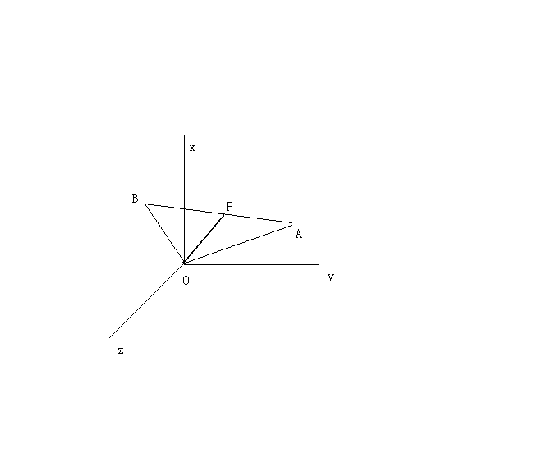
\includegraphics[scale=0.6]{gto.eps}\label{BASIS:1}
      \caption{the center theorem related to GTO}
    \end{center}
  \end{figure}

  If there's two center GTO orbital, one is residing on A, and the
  other is residing on B; we can prove that the multiplication of the
  two GTOs can be transformed into a one center of GTO, who is located
  in center of P (see the \ref{BASIS:1}).

  Thus we have:
  \begin{equation}\label{}
    exp(-ar_{A}^{2})exp(-br_{B}^{2}) = Kexp(-ar_{p}^{2})
  \end{equation}

\end{comment}

%%%%%%%%%%%%%%%%%%%%%%%%%%%%%%%%%%%%%%%%%%%%%%%%%%%%%%%%%%%%%%%%%%%%%%%%%%
\section{Contracted Gaussian type orbitals}
%
% to use the gaussian function, people always to contract them
% together to form the basis sets.  what's the relation between GTO
% and basis sets?  how to contract them to form the basis sets?
% introduce the two different way of contracting: segmental and
% general way
%
Gaussian primitives are usually obtained from quantum calculations on
atoms (i.e. Hartree-Fock or Hartree-Fock plus some correlated
calculations, e.g. CI). Typically, the exponents are varied until the
lowest total energy of the atom is achieved. In some cases, the
exponents are optimized independently. In others, the exponents are
related to each other by some equation, and parameters in this
equation are optimized (e.g. even-tempered or "geometrical" and
well-tempered basis sets). The primitives so derived describe isolated
atoms and cannot accurately describe deformations of atomic orbitals
brought by the presence of other atoms in the molecule.  Basis sets
for molecular calculations are therefore frequently augmented with
other functions, which has smaller exponent and able to describe the
motion of electrons far away from the nucleus.

For molecular calculations, these gaussian primitives have to be
contracted, i.e., certain linear combinations of them will be used as
basis functions. The term contraction means "a linear combination of
gaussian primitives to be used as basis function".  Such a basis
function will have its coefficients and exponents fixed. The
contractions are sometimes called Contracted Gaussian Type Orbitals
(CGTO). For instance, there's a four s-type gaussian primitives used
to represent 1s orbital of hydrogen as:
\begin{multline}\label{}
  \varphi_{1s} = 0.50907N_{1}e^{-0.123317r^{2}} +
  0.47449N_{2}e^{-0.453757r^{2}} \\
  + 0.13424N_{3}e^{-2.01330r^{2}} + 0.01906N_{4}e^{-13.3615r^{2}}
\end{multline}
$N_{i}$ is a normalization constant for a given primitive. In the case
of gaussian primitives of type s it is equal to
$(2\alpha/\pi)^{\frac{3}{4}}$.

These primitives may be grouped in 2 contractions. The first
contraction contains only 1 primitive:
\begin{equation}\label{}
  \phi_{1} = Ne^{-0.123317r^{2}}
\end{equation}

3 primitives are present in the second contraction:
\begin{multline}\label{}
  \phi_{2} = N[0.47449N_{2}e^{-0.453757r^{2}} +
  0.13424N_{3}e^{-2.01330r^{2}} \\
  + 0.01906N_{4}e^{-13.3615r^{2}}]
\end{multline}

N is a normalization constant for the whole contraction.

In this case, 4 primitives were contracted to 2 basis functions. It is
frequently denoted as $(4s) \rightarrow [2s]$ contraction (some use
(4s)/[2s] notation). The coefficients in function $\phi_{2}$ are then
fixed in subsequent molecular calculations.

Obviously, the best results could be obtained if all coefficients in
gaussian expansion were allowed to vary during molecular
calculations. Moreover, the computational effort (i.e. "CPU time") for
calculating integrals in the Hartree-Fock procedure depends upon the
4th power in the number of gaussian primitives. However, all
subsequent steps depend upon the number of basis functions (i.e.
contractions). Also, the storage required for integrals (when Direct
SCF is not used) is proportional to the number of basis functions (not
primitives!). Frequently the disk storage and not the CPU time is a
limiting factor. The CPU time requirements are more acute when
post-Hartree- Fock (e.g. correlated methods) are used, since the
dependance upon the number of basis functions here is more steep than
the 4th power.

There are two basic forms of contractions, namely "segmented" and
"general". The segmented contractions are disjointed, i.e., given
primitive appears only in one contraction. The example given above
$(4s) \rightarrow [2s]$ is a segmented contraction. Occasionally, one
or two primitives may appear in more than one contraction, but this is
an exception to the rule. The general contractions, on the contrary,
allow each of the primitives to appear in each basis function
(contraction). The segmented contractions are far more popular and
will be described first. The reason for their popularity is not that
they are better, but simply, that the most popular ab initio packages
do not implement efficient integral calculations with general
contractions. The computer code to perform integral calculations with
general contractions is much more complex than that for the segmented
case.

%%%%%%%%%%%%%%%%%%%%%%%%%%%%%%%%%%%%%%%%%%%%%%%%%%%%%%%%%%%%%%%%%%%%%%%%%
\subsection{Segmented basis sets}
%
% how to form the segmented basis sets? there's some rules: 1 the
% inner part is assigned with less flexibility (less basis sets), but
% more GTO used to get a better shape (such as 6-31g, use 6 GTOs to
% simulate the inner shell, but only three the the outer ones) 2 the
% outer ones are assigned with better flexibility (more basis sets) so
% that to make the basis sets more adaptable to the change of
% molecular environments.  3 also the polarized function and diffuse
% functions are used. they are always left uncontracted, since that
% they are not derived from the atom calculation.  these functions are
% used to help the basis set to change more flexible.
%
The segmented basis sets are usually structured in such a way that the
most diffuse primitives (primitives with the smallest exponent) are
left uncontracted (i.e. one primitive per basis function). More
compact primitives (i.e. those with larger exponents) are taken with
their coefficients from atomic Hartree-Fock calculations and one or
more contractions are formed. Then the contractions are renormalized.

Cartesian gaussian primitives are grouped in shells corresponding to
the same value of angular momentum quantum number. Of course, these
shells should not be confused with electron shells (i.e. electrons
with the same principal quantum number: $K \rightarrow n=1$, $L
\rightarrow n=2$, etc.). So as to avoid the ambiguity, we use s-shell,
p-shell, d-shell, f-shell, g-shell, etc. to signal the shell of
gaussian primitives. The shell is a collection of cartesian gaussian
primitives that have the same L (see definition of cartesian gaussian
above). Strictly speaking, the s-shell is a collection of s type
gaussian primitives; p-shell is a collection of p-type gaussian
primitives; d-shell is a collection of d-type gaussian primitives; and
so on. Of course, combining primitives belonging to different shells
within the same contraction does not make sense because primitives
from different shells are orthogonal.

But even here there is a room for more confusion. Many basis sets use
the same exponents for functions corresponding to the same principal
quantum number, i.e., electronic shell. 3-21g is an example, as well
as other basis sets from Pople's group. Atoms of the first and second
row (i.e. Li - Ne, Na - Cl) have the same exponents for s- and p-type
gaussian primitives formally associated with a given electron shell of
the isolated atom. For the basis sets in which s- and p-type functions
share the same exponents, the term SP-shell is used (here in the
output job file by Gaussian03, this is clearly
demonstrated). Sometimes term L-shell is used by analogy to the 2nd
electron shell. This approximation works very well in
practice. Moreover, it is possible to write efficient code for
calculating integrals for such cases. It is important to stress here
that the distinction between inner orbitals and valence orbitals is
kind of carry-over from the past era of Slater orbitals.  Contractions
consisting of primitives with large exponents are associated with
inner atomic orbitals while more diffuse functions are allied with
valence orbitals. Basis functions are not usually atomic orbitals, and
in many cases, they do not even resemble orbitals of isolated
atoms. In fact, examining coefficients of molecular orbitals
frequently reveals that these "core" basis functions contribute
substantially to the Highest Occupied Molecular Orbital (HOMO). It
comes as a consequence of the fact that basis functions on a given
center are usually not orthogonal to each other and "core" basis
functions on different centers overlap to a great extent - situation
not likely to occur with true atomic orbitals.

The early gaussian contractions were obtained by a least square fit to
Slater atomic orbitals. The number of contractions (not primitives!)
used for representing a single Slater atomic orbital (i.e. zeta) was a
measure of the goodness of the set. From this era we have terms like
single zeta (SZ), double zeta (DZ), triple zeta (TZ), quadruple zeta
(QZ), etc. In the minimal basis set (i.e. SZ) only one basis function
(contraction) per Slater atomic orbital is used. DZ sets have two
basis functions per orbital, etc. Since valence orbitals of atoms are
more affected by forming a bond than the inner (core) orbitals, more
basis functions are assigned frequently to describe valence
orbitals. This prompted development of split-valence (SV) basis sets,
i.e., basis sets in which more contractions are used to describe
valence orbitals than core orbitals. That more basis functions are
assigned to valence orbitals does not mean the valence orbitals
incorporate more primitives.  Frequently, the core orbitals are long
contractions consisting of many gaussian primitives to represent well
the "cusp" of s type function at the position of the nucleus. The
"zeta" terminology is often augmented with a number of polarization
functions which will be described later. So, DZP means double-zeta
plus polarization, TZP stands for triple-zeta plus polarization,
etc. Sometimes the number of polarization functions is given,
e.g. TZDP, TZ2P, TZ+2P stands for triple-zeta plus double
polarization. Letter V denotes split valence basis sets, e.g., DZV
represents basis set with only one contraction for inner orbitals, and
two contractions for valence orbitals. The creativity here is enormous
and spontaneous.

The minimal basis set is the smallest possible set, i.e., it contains
only one function per occupied atomic orbital in the ground
state. Actually, it always includes all orbitals from partially
occupied sub shells and valence p-type functions for elements from the
first 2 groups of the periodic table. So for Li and Be atoms it has 2
s-type contractions and 1 p-type contraction. Minimal basis set for S
atom has 3 s-type contractions and 2 p-type contractions.  The most
popular minimal basis sets are the STO-nG, where n denotes number of
primitives in the contraction. These sets were obtained by least
square fit of the combination of n gaussian functions to a Slater type
orbital of the same type with zeta = 1.0, For this set additional
constraint is used, that exponents of corresponding gaussian
primitives are the same for basis functions describing orbitals with
the same principal quantum number (e.g. the same primitives are used
for 2s and 2p function).For the minimal basis set, the STO-3G (i.e. 3
primitives per each function) is the most widely used set.

For other sets a more complicated notation needs to be used to specify
the number of primitives and contractions explicitly. The parentheses
() embrace the number of primitives that are given in the order of
angular momentum quantum number. Square brackets [] are used to
specify the number of resulting contractions. For example: (12s,9p,1d)
means 12 primitives on s-shell, 9 primitives on p-shell, and 1
primitive on d-shell. This is sometimes abbreviated even further by
skipping the shell symbols (12,9,1). The [5,4,1] means that s-shell
has 5 contractions, p-shell has 4 contractions and d-shell has 1
contraction. To denote how contractions were performed, the following
notation is frequently used: $(12,9,1) \rightarrow [5,4,1]$ or
$(12,9,1)/[5,4,1]$ or $(12s,9p,1d) \rightarrow [5s,4p,1d]$. This means
that 12 s-type primitives were contracted to form 5 s-type
contractions, 9 p-primitives were contracted to 4 basis functions and
1 d-primitive was used as a basis function by itself. Note of caution
here. The statement "9 p-primitives were contracted to 4 basis
functions" actually means that 12 basis functions were created. Each
p-type basis functions has 3 variants: $p_{x}, p_{y}, p_{z}$ which
differ in their cartesian part (i.e., angular part). The same is true
for d-, f-, and higher angular momentum functions.

%%%%%%%%%%%%%%%%%%%%%%%%%%%%%%%%%%%%%%%%%%%%%%%%%%%%%%%%%%%%%%%%%%%%%%%%
\subsection{Basis sets in computation}
%
% 1 importance in the understanding of the quantum chemistry codes 2
% introduce the primitive shells, and to see the difference between
% the gaussians and the primitive shells.  3 basis sets are linear
% combination of the primitive shells 4 shells concept 5 what should
% be contained in the quantum chemistry program
%
%
To some extent, basis sets is the foundation of the codes in the
quantum chemistry, it's impossible to understand any quantum chemistry
codes without the understanding of the basis sets. Hence, in this
section we hope to give some basic concept of how to express the basis
sets in the quantum chemistry codes. Here the examples are all from
the Gaussian program, but other programs share the similar ideas so
that it's easy to derive the others forms.

In the quantum chemistry program, it's a trivial way to store all the
basis sets information by the form of gaussian functions, in the
context below; we can see that it's some way too verbose. On the
contrary, it's convenient to contract the information inside the
gaussian functions to form some "compact" expressions, they are more
suitable to store in the computer and the information is easy to
extract from them. That's what we called the shells and the primitive
shells.

The primitive shells are defined as the set of gaussian functions
which share the same exponents and the same maximum quantum angular
number. For example, the $2s$, $2px$, $2py$ and $2pz$ are considered
to be the same primitive shell, but $1s$, $3d$ gaussian functions are
not in this primitive shell because they have different angular part.

Since that the $S$ type gaussian and $P$ type gaussian are always to
be made to share the same primitive shell, should we follow the same
way to deal with the $D$ orbital and even $F$ orbitals? But there's an
problem; that if people want to calculate the molecules containing the
$d$ orbitals; all the $S$, $P$ and $D$ gaussian functions in the same
shell will be introduced together (if the $d$ orbital is introduced as
some polarized functions, we do not want to do the work in this way);
thus some way need to devised to avoid this situation.

Therefore, for the higher angular momentum part of gaussian functions
(namely the $d$ type and the $f$ type), we use the constraint shells
instead; that is in these shells, only the $d$ or $f$ functions are
inside to form the primitive shells. The only difference related to
these shells is only that to use the pure form or the cartesian
form. For the $d$ type of orbitals, the pure type owns only five
orbitals, whereas the cartesian type has six orbitals; these has been
discussed in the above content.

In the real program, so far people always use the the $SP$ shell to
represent the $s$ type and $p$ type gaussians (thus they share the
same exponents), this is popular in the Pople basis sets; but in other
kind of basis sets such as the Dunning basis sets, the $s$ and $p$ are
separated to be into different primitive shells.

At last let's give some example. Take the oxygen atom of the $6-31g$
as an example, the $6$ gaussians are the six primitive shells (they
have different exponents), they are composed into the basis function
which characterizes the inner orbital of $1s$. On the other hand, the
other $3$ gaussians and additional one gaussians form the other two
group of primitive shells, each one represents the $2s$, $2px$, $2py$
and $2pz$, separately. Thus the ten primitive shells represents $9$
basis sets and contain $14$ gaussian functions.

Now we can see that if we use the pure gaussian functions instead,
it's some too wordy way since that different $px$ $py$ and $pz$ are
take into account. Therefore, in the quantum chemistry the primitive
shells are used as the elementary brick to construct the storing whole
basis sets.

Next, the basis sets are considered to be the linear combination of
the same type of the primitive shells. Thus the basis sets consist of
the same type of angular part. In quantum chemistry, the basis sets is
the most elementary components, the function space are formed from the
variation of the basis sets.

Finally, shells are the most abstract concept. The shell is considered
to contains the same type of primitive shells, they share the same
angular momentum number. For example, $S$ shell, $P$ shell or $D$
shell. It can see that the concept of shell is larger than the basis
sets. For example, the basis of $6-31g$ use two different basis sets
to represent the same type of shell (if for oxygen atom, it's the $SP$
shell; if for the $Br$ atom, it's the $3d$, $4s$ and $4p$ shell).

At last, we try to list the data information used in the common
quantum chemistry package. All the basis sets information, is actually
contracted into the shell array (also the primitive shell array). Here
below is the necessary part of these arrays:
\begin{itemize}
\item for each shell, what kind of atom it belongs to.
\item for each shell, the starting point of its gaussian functions
  list. For example, O atom with $6-31g$ basis set has three shells
  $(1s, 2sp, 3s^{'}p^{'})$. $1s$ has six primitives, thus $array(1) =
  1$, $array(2) = 7$. In this way we can determine the number of
  gaussians it contains.
\item the number of gaussians for each shell.
\item for each shell, what is its angular part? $S$, $SP$ or $D$?
\item For the $D$ or $F$, we use the pure ones or cartesian ones?
\item total shell number
\item the maximum angular type
\item the exponent array, and the corresponding coefficients for the
  primitive shells
\end{itemize}

%%%%%%%%%%%%%%%%%%%%%%%%%%%%%%%%%%%%%%%%%%%%%%%%%%%%%%%%%%%%%%%%%%%%%%%%%%
\subsection{Pople's Basis Sets}
A different convention was adopted by Pople and coworkers. The basis
set structure is given for the whole molecule, rather than particular
a atom. This notation emphasizes also a split valence (SV) nature of
these sets. Symbols like n-ijG or n-ijkG can be encoded as: n - number
of primitives for the inner shells; ij or ijk - number of primitives
for contractions in the valence shell. The ij notations describes sets
of valence double zeta quality and ijk sets of valence triple zeta
quality. Generally, in basis sets derived by Pople's group, the s and
p contractions belonging to the same "electron shell"
(i.e. corresponding formally to the same principal quantum number n)
are folded into a sp-shell. In this case, number of s-type and p-type
primitives is the same, and they have identical exponents. However,
the coefficients for s- and p-type contractions are different.

Now, we are giving some examples. The 4-31G basis set for hydrogen
(hydrogen has only valence electrons!) is a contraction $(31)$ or
$(4s)\rightarrow[2s]$; for first row atoms $(8s,4p) \rightarrow
[3s,2p]$; and for 2nd row atoms the contraction scheme is $(12s,8p)
\rightarrow [4s,3p]$. The 6-311G set represents the following
contractions for water is $(11s,5p/5s) \rightarrow [4s,3p/3s]$.

The Pople's basis sets can also be augmented with d type polarization
functions on heavy atoms only (n-ijG* or n-ijkG*) or on all atoms,
with p-functions on hydrogens (n-ijG** or n-ijkG**). In methane, the
4-31G* encodes following split $(8s,4p,1d/4s) \rightarrow
[3s,2p,1d/2s]$, while 6-311G** for HCN molecule would involve
following contractions: $(11s,5p,1d/5s,1p) \rightarrow
[4s,3p,1d/3s,1p]$.




%%% Local Variables:
%%% mode: latex
%%% TeX-master: "../../main"
%%% End:

%\chapter{General Discussion to Configuration Interation Methods}
%
%
%
%
\section{The Limitation of The HF Theory}
%
% does not include the correlation effects how to understand the
% correlation effects, in the pictured way Pauli effects and
% correlation effects
%
On the base of single electron approximation, the Hatree-Fock theory
succeeds in making good approximation to the schrodinger equation.  In
a sufficiently large basis sets, the HF wave function can account for
$99$ percent of the total energy. However, the remaining $1$ percent
is always fatal in describing chemical phenomenon.

What does the error in HF theory come from? Generally to say, this is
due to the single electron approximation. As the quantum law declares
that there's correlation between quantum particles (electron is surely
included in), it's impossible for the quantum particles to move in an
irrelevant way. More specifically, here we can give a naive but easily
understood description.

As a result of HF calculation, the electrons are grouped in pair to
reside in the HF orbitals, starting from the orbital with lowest
energy. Thus, for a closed shell system, each orbital are taken by
pair of electrons with opposite spin. The spatial overlap between such
pair of electrons is exactly one, while the overlap between two
electrons belonging to different orbitals is exactly zero because of
the orthogonality.

Naively to say, this can not be true. For electrons are quantized,
it's impossible for two pair of electrons to share exactly the same
orbital, only different in spin. When one electron moves, the other
must be "correlated". This holds true for electrons in different
orbitals, too. Their moving is correlated so that the orthogonality is
only a kind of approximation.

The difference between the exact ground state energy and the HF energy
(under the non relativistic condition and the Born-Oppenheimer
approximation) is called \textbf{electron correlation energy}. To some
extent, such correlation is called coulomb correlation, it arises
between electrons in opposite spin among orbitals, for the pauli
principle has the consequence that there is no intraorbital
correlation from electron pairs with same spin. The correlation
attributed to the pauli principle, is called Fermi correlation; which
has been exactly contained in the HF theory.

If we want to contain the correlation energy, we have to step into the
CI (configuration interaction ) method.

%%%%%%%%%%%%%%%%%%%%%%%%%%%%%%%%%%%%%%%%%%%%%%%%%%%%%%%
\section{How to Form The CI Wave Functions}\label{CI2}
%
% 1 requirement to form the wave functions 2 the requirement for the
% basis functions 3 use the permutation operator to express the
% permutation process to the orbital 4 get the determinant form
%
the first question in the CI method, is that how to form the wave
functions. Firstly we note that such wave functions should satisfy two
points:
\begin{itemize}
\item wave functions should be arisen from a complete set of basis
  functions
\item wave functions should satisfy the anti-symmetric properties
  while exchanging electrons
\end{itemize}

In general, we can have many ways to realize such construction
satisfying the requirements above. For example, the linear combination
of plane waves. However, in quantum chemistry, we always use the
spin-orbitals as the basis functions, that is:
\begin{equation}\label{}
  \varphi_{A}(r,s), \varphi_{B}(r,s), \cdots, \varphi_{X}(r,s)
\end{equation}
Here on each orbital there may has electron residing on it (which is
called occupied orbital); or no electrons residing on it (so called
virtual orbital). The total $N$ electrons are considered to be
distributing over such set of basis functions, each one is orthogonal
with the other and satisfying the normalized condition.  Here we note
that generally we do not care how the orbitals we can get, but usually
they are gotten from HF calculation; but here we only consider the
general character of the basis functions, which is required to be
complete, orthogonal and normalized.

Then the question is: how to build the wave functions based on such
series of $\varphi_{k}$ ($k = A, B, \cdots, X$)?

First, generally we can the total wave function of $\Phi$ expressed
as:
\begin{equation}\label{}
  \Phi = \sum_{A,B, \cdots, X}C_{AB\cdots
    X}\varphi_{A}\varphi_{B}\cdots\varphi_{X}
\end{equation}
Then, for a given set of spin-orbitals, that is the $A, B, \cdots, X$
are fixed to be certain; we can see that the electrons label are
totally arbitrary. The electron $1$ can be considered to be setting on
the $\varphi_{A}$, or $\varphi_{B}$; which does not change the whole
wave function of $\Phi$.

Therefore, we can use some permutation operator of $\hat{P}$ (more
discussion can see the quantum mechanics part, the chapter related to
the identity particle), which is used to change all the $N$ electrons
among the $A, B, \cdots, X$ orbitals:
\begin{equation}\label{}
  \hat{P} = \prod_{1\leq i<j\leq N}\hat{P}_{ij}
\end{equation}
Here the $\hat{P}_{ij}$ is the exchange operator for exchanging the
electron $i$ and $j$. Hence, we can have:
\begin{align}\label{}
  \hat{P}\Phi &= (-1)^{P}\Phi \Rightarrow \nonumber \\
  \Phi &=\sum_{A,B, \cdots, X}C_{AB\cdots
    X}(-1)^{-P}\hat{P}\{\varphi_{A}\varphi_{B}\cdots\varphi_{X}\}
  \nonumber \\
  &=\sum_{A,B, \cdots, X}C_{AB\cdots
    X}(-1)^{P}\hat{P}\{\varphi_{A}\varphi_{B}\cdots\varphi_{X}\}
  \nonumber \\
\end{align}
Here from the definition of $P$ we surely have $(-1)^{-P} = (-1)^{P}$.

From mathematics, it's clear to know that such permutation can be
equivalently expressed as determinant, thus we finally have:
\begin{equation}\label{CIeq:26}
  \Phi = \sum_{A,B, \cdots, X}C_{AB\cdots X}
  \frac{1}{\sqrt{N!}}\begin{vmatrix}
    \varphi_{A}(1) & \varphi_{A}(2) & \cdots & \varphi_{A}(n) \\
    \varphi_{B}(1) & \varphi_{B}(2) & \cdots & \varphi_{B}(n) \\
    \cdots & \cdots & \cdots & \cdots \\
    \varphi_{X}(1) & \varphi_{X}(2) & \cdots & \varphi_{X}(n) \\
  \end{vmatrix}
\end{equation}
Therefore, by changing the $A,B, \cdots, X$, for example; to change
the $A$ orbital into the $Y$ orbital; we will get another
determinant. Then their linear combination is finally forming the wave
functions.

Finally, we note that the form of (\ref{CIeq:26}) is general. It's not
only for HF orbitals, but also for any other basis functions used to
constructing the CI wave function. From this concept, we can naturally
have the impression about the root determinant and the exciting
determinants; as what will be mentioned below.


%%%%%%%%%%%%%%%%%%%%%%%%%%%%%%%%%%%%%%%%%%%%%%%%%%%%%%%%
\section{Basic Idea in CI Algorithm}
%
% 1 address the idea of the variational process 2 introduce the
% concept of configuration
%
%
The main idea for the CI, is very simple and straightforward; that is
only based on the variational principle.

The variational principle states that if we have a set of approximate
wave function (usually it's the determinants of what we have just
talked about), which is complete, orthogonal and normalized; the
linear combination of the approximate wave function can have an energy
which is above or equal to the exact energy. In the following content,
we will give a demonstration of the theory.

We can use the variational principle in this way: first construct an
approximate wave function of $\Psi$, which satisfies the condition of
the exact wave function, but has some flexible parameters as $a_{1},
a_{2}, \cdots, a_{l}$; so the above variational principle can write
as:
\begin{eqnarray} \label{CIeq:1}
  % \nonumber to remove numbering (before each equation)
  E(a_{1}, a_{2}, \cdots, a_{l}) &=&  \frac{\langle \Psi|\hat{H}| \Psi
    \rangle} {\langle \Psi|\Psi \rangle} \nonumber \\
  & \geq & E_{0}
\end{eqnarray}

Then we can properly choose the flexible parameters of $a_{1}, a_{2},
\cdots, a_{l}$ so that to make $E(a_{1}, a_{2}, \cdots, a_{l})$ is a
minimum. Here the minimum energy is as the upper boundary of the true
energy, and the difference between them depends on the quality of the
approximate wave function we use. The set of flexible parameters are
required as:
\begin{equation}\label{CIeq:2}
  \frac{\partial E(a_{1}, a_{2}, \cdots, a_{l})}{\partial a_{k}} = 0
  (k= 1,2, \cdots, l)
\end{equation}

In CI calculation, we always choose the linear combination of the
slater determinants as the approximate wave function, each of the the
approximate slater determinant is called "configuration".

The slater determinants are formed from a HF calculation. After the HF
calculation, we can get a set of HF occupied orbitals and virtual
orbitals. By firing the electrons on the occupied orbital onto the
virtual orbital, we can get the excited slater determinant. So sorted
by the electrons fired up onto the virtual orbitals, we have singly,
doubly, triply etc. excited relative to the ground HF determinant. the
illustration of the excited determinants can see the figure of
(\ref{CI1}).Their combination can be written as:
\begin{equation}\label{CIeq:3}
  \Psi_{CI} = a_{0}\Psi_{HF} + \sum _{S}a_{S}\Psi_{S} + \sum
  _{D}a_{D}\Psi_{D} + \sum _{T}a_{T}\Psi_{T} + \cdots
\end{equation}

\begin{figure}[htp]
  \begin{center}
    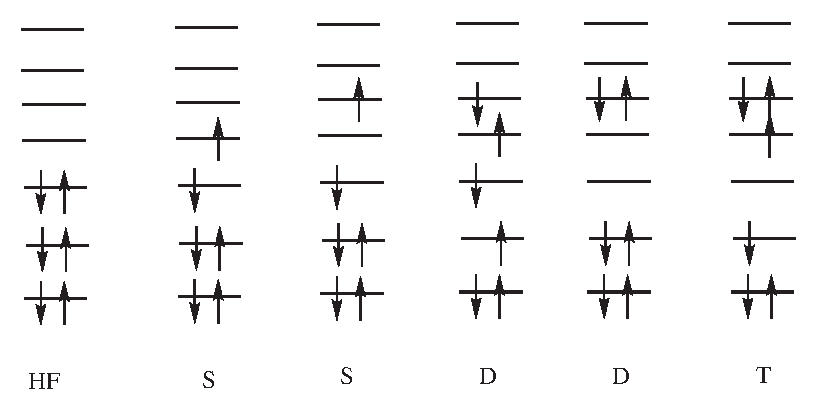
\includegraphics[scale=1.0]{ci.eps}\label{CI1}
    \caption{illustration of the excited determinants}
  \end{center}
\end{figure}

Before the deduction of the variational principle, it's appropriate
for us to make an outline of this method, and specify some important
points.

In the CI methods, first we run HF calculation, then we form the
configurations; finally we can get the CI wave function by energy
minimization. Thus this method is two-dimensional, the size of HF
orbitals (which is determined by the size of the basis sets), and the
number of determinants; are the two loosely independent factors that
influencing the result of the CI calculation.

Therefore, the larger of the basis sets, and the larger number of the
slater determinants; the more better result that the CI calculation
can achieve.

It's worthy to note here, that the CI method includes the exact Fermi
correlation, which is the same as the HF theory.

This point is important, but very easy to prove. As shown in the
(\ref{CIeq:3}), we can write the CI wave function as:
\begin{equation}\label{}
  \Phi_{CI} (1,2,\cdots, n) = \sum _{i}a_{i}\Psi_{i} (1,2,\cdots, n)
\end{equation}
If we interchange electron k,l in the $\Psi_{i} (1,2, \cdots, k,l,
\cdots, n)$ to make it become $\Psi_{i} (1,2, \cdots, l,k, \cdots, n)$
for all the determinants $i=1,2, \cdots, n$; that leads to the
$-\Psi_{CI}(1,2,\cdots, n)$; which is equivalent to interchange
electrons k,l in the $\Psi_{CI}$.


%%%%%%%%%%%%%%%%%%%%%%%%%%%%%%%%%%%%%%%%%%%%%%%%%%
\section{Variational Process in CI}
%
%
%
%
So now we can go to prove the variational process used in the CI
algorithm. This general derivation is taken from Tang's
book\cite{aoqingTang}, and I favor this demonstration for it's
clearness and simplicity. Here in the following content, the $\Phi$ is
designated as the CI wave function, and the $\Psi$ is designated as
the slater determinant; we do so just because in the HF chapter the
$\Psi$ is designated as the HF wave function (the root slater
determinant).

Based on the variational principle, we can express any CI wave
function by this way:
\begin{equation}\label{CIeq:4}
  \Phi = \sum_{j}c_{j}\Psi_{j}
\end{equation}
So by inserting this expression into the schrodinger function, we
have:
\begin{equation}\label{CIeq:5}
  \sum_{j}c_{j}\hat{H}\Psi_{j} = E\sum_{j}c_{j}\Psi_{j}
\end{equation}

By multiplying the left bra of $\langle\Phi|$, which is actually
expressed as $\sum_{i}c_{i}^{*}\Psi_{i}$; we have:
\begin{equation}\label{CIeq:6}
  \sum\limits_{i}\sum\limits_{j}c_{i}^{*}c_{j}\langle\Psi_{i}|\hat{H}|\Psi_{j}\rangle
  =E\sum\limits_{i}\sum\limits_{j}c_{i}^{*}c_{j}\langle\Psi_{i}|\Psi_{j}\rangle
\end{equation}

Which finally yields:
\begin{equation}\label{CIeq:7}
  E=\frac{\sum_{i}\sum_{j}c_{i}^{*}c_{j}\langle\Psi_{i}|\hat{H}|\Psi_{j}\rangle}
  {\sum_{i}\sum_{j}c_{i}^{*}c_{j}\langle\Psi_{i}|\Psi_{j}\rangle}
\end{equation}

as we make a bit change to $c_{i}^{*}$, make it to $c_{i}^{*}+\delta
c_{i}^{*}$, here the right ket of $|\Phi\rangle$ is also changed.
Hence the $E$ is changed to the $E+\delta E$; so we have:
\begin{equation} \label{CIeq:8} E+\delta E =
  \frac{\sum_{i}\sum_{j}(c_{i}^{*}+\delta c_{i}^{*})(c_{j}+\delta
    c_{j}) \langle\Psi_{i}|\hat{H}|\Psi_{j}\rangle}
  {\sum_{i}\sum_{j}(c_{i}^{*}+\delta c_{i}^{*})(c_{j}+\delta c_{j})
    \langle\Psi_{i}|\Psi_{j}\rangle}
\end{equation}

The expression above is a bit wordy, so we rewrite it into a
compressed form:
\begin{equation}\label{CIeq:9}
  E+\delta E = \frac{(C+\delta C)^{*}H(C+\delta C)}{(C+\delta C)^{*}M(C+\delta C)}
\end{equation}
In the expression above, the $C$ is the compression of $\sum c_{i}$,
and $H$ is the matrix of $\langle\Psi_{i}|\hat{H}|\Psi_{j}\rangle$;
that is:
\begin{equation}\label{CIeq:10}
  \left [ \begin{array}{cccc}
      \langle\Psi_{1}|\hat{H}|\Psi_{1}\rangle & \langle\Psi_{1}|\hat{H}|\Psi_{2}\rangle & \cdots & \langle\Psi_{1}|\hat{H}|\Psi_{n}\rangle \\
      \langle\Psi_{2}|\hat{H}|\Psi_{1}\rangle & \langle\Psi_{2}|\hat{H}|\Psi_{2}\rangle & \cdots & \langle\Psi_{2}|\hat{H}|\Psi_{n}\rangle \\
      \cdots & \cdots & \cdots & \cdots                                  \\
      \langle\Psi_{n}|\hat{H}|\Psi_{1}\rangle & \langle\Psi_{n}|\hat{H}|\Psi_{2}\rangle & \cdots & \langle\Psi_{n}|\hat{H}|\Psi_{n}\rangle
    \end{array} \right ]
\end{equation}

the $M$ is similar to the $H$, which has no $\hat{H}$. So as the
(\ref{CIeq:8}) is compressed into the matrix form, the meaning is more
clear.

From (\ref{CIeq:9}) we have:
\begin{equation}\label{CIeq:11}
  E + \delta E = \frac{C^{*}HC + \delta C^{*}HC + C^{*}H \delta C + \delta C^{*}H \delta C }
  {C^{*}MC + \delta C^{*}MC + C^{*}M \delta C + \delta C^{*}M \delta C}
\end{equation}
We omit all the second order infinitesimal, and we have:
\begin{equation}\label{CIeq:12}
  E + \delta E = \frac{1}{C^{*}MC} \frac{C^{*}HC + \delta C^{*}HC + C^{*}H \delta C }
  { 1+ \frac{\delta C^{*}MC + C^{*}M \delta C}{C^{*}MC}}
\end{equation}
Furthermore to expand this math expression to infinite series and omit
the second order infinitesimal, we can write:
\begin{equation}\label{CIeq:13}
  \frac{1}{ 1+ \frac{\delta C^{*}MC + C^{*}M \delta C}{C^{*}MC} } = 1
  - \frac{\delta C^{*}MC + C^{*}M \delta C}{C^{*}MC}
\end{equation}


So we have:
\begin{equation}\label{CIeq:14}
  E + \delta E = \frac{C^{*}HC + \delta C^{*}HC + C^{*}H \delta
    C}{C^{*}MC} * (1 - \frac{\delta C^{*}MC + C^{*}M \delta C}{C^{*}MC})
\end{equation}

By remembering that $E=\frac{C^{*}HC}{C^{*}MC}$, and also omit the
second order infinitesimal; we finally have this expression:
\begin{equation}\label{CIeq:15}
  \delta C^{*}HC + C^{*}H \delta C - E(\delta C^{*}MC + C^{*}M \delta
  C) = 0
\end{equation}
Here we drop the denominator for the $C^{*}MC$ is always larger than
0.

From the expression above, by separating the two different
infinitesimal, which are $\delta C^{*}$ and $\delta C$; we can get
that:
\begin{eqnarray}\label{CIeq:16}
  % \nonumber to remove numbering (before each equation)
  \delta C^{*}(HC-EMC)  &=& 0 \nonumber \\
  (C^{*}H-EC^{*}M)\delta C&=& 0
\end{eqnarray}
And actually they are the same. We can transpose one to the another.
So finally we get the answer:
\begin{equation}\label{CIeq:17}
  HC=EMC
\end{equation}

If we select the Slater determinants as the reference for expansion, then it's
easy to know that:
\begin{equation}
 M_{ij} = \delta_{ij} 
\end{equation}
so we have $HC=EC$. By diagonal we can the energy.

%%%%%%%%%%%%%%%%%%%%%%%%%%%%%%%%%%%%%%%%%%%%%%%%%%%%%%
\section{CI Matrix Elements}
After setting up the general algorithm of the CI, next step we are
going to introduce some simple rules to evaluate its matrix
elements. Here the evaluation is only related to the spatial part of
the orbital, so only the singly excited determinant of S, and D, T,
etc. are concerned into this part.

%%%%%%%%%%%%%%%%%%%%%%%%%%%%%%%%%%%%%%%%%%%%%%%%%%%%%%
\subsection{Brillouin's Theorem}
%
% simple statement about this theorem
%
Brillouin's theorem is a simple and direct result of HF theory, it
states that the overlap between the ground state configuration of
$|\Psi \rangle$ and the singly excited determinant of $|\Psi^{r}
\rangle$ (in which one of occupied orbital of $\varphi_{s}$ has been
replaced by an unoccupied orbital of $\varphi_{r}$, so we designated
this configuration as $|\Psi^{r} \rangle$) is zero, that means to
include the singly excited determinant into the root determinant has
no contribution to the ground state energy.

So we can prove it. Suppose that the CI wave function is written as:
$|\Phi \rangle= a_{0}|\Psi \rangle+ a_{1}|\Psi^{r}\rangle$, here we
have the $|\Psi \rangle$ just as the determinant we use in the
(\ref{HFTeq:20})(HF theory chapter); so the CI matrix of $H$ just
showed in the (\ref{CIeq:17}) can be written as:
\begin{equation}\label{CIeq:19}
  \left[
    \begin{array}{cc}
      \langle \Psi|\hat{H}|\Psi     \rangle       &   \langle \Psi|\hat{H}|\Psi^{r}     \rangle     \\
      \langle \Psi^{r}|\hat{H}|\Psi \rangle       &   \langle \Psi^{r}|\hat{H}|\Psi^{r} \rangle     \\
    \end{array}
  \right]
\end{equation}
Now we concentrate on the matrix element of $\langle
\Psi^{r}|\hat{H}|\Psi\rangle$, which finally turns out to be 0.

Similar to the (\ref{HFTeq:21}), we can write the schrodinger operator
as:
\begin{equation}\label{CIeq:20}
  \hat{H} = \sum_{i}^{n}h_{i} + \sum_{i<j}^{n}J_{ij}
\end{equation}
here the $h_{i}$ denotes the single electron operator, and the
$J_{ij}$ denotes the double electrons operator. So we have:
\begin{eqnarray}\label{CIeq:21}
  % \nonumber to remove numbering (before each equation)
  \langle \Psi^{r}|\hat{H}|\Psi\rangle &=&
  \langle \Psi^{r}|\{\sum_{i}^{n}h_{i}
  + \sum_{i<j}J_{ij} \}|\Psi\rangle      \nonumber \\
  &=& n\langle\Psi^{r}|h_{1}|\Psi\rangle + C_{n}^{2}\langle\Psi^{r}|J_{12}|\Psi\rangle
\end{eqnarray}

The (\ref{CIeq:21}) can be further transformed into the expression
below(here the $\hat{f}$ is the HF operator):
\begin{multline}\label{CIeq:22}
  n\langle\Psi^{r}|h_{1}|\Psi\rangle +
  C_{n}^{2}\langle\Psi^{r}|J_{12}|\Psi\rangle = \langle\varphi_{r}(1)|h_{1}|\varphi_{s}(1)\rangle +  \\
  \sum_{i \neq s} \left\{
    \langle\varphi_{r}(1)\varphi_{i}(2)|J_{12}|\varphi_{s}(1)\varphi_{i}(2)\rangle
    -
    \langle\varphi_{r}(1)\varphi_{i}(2)|J_{12}|\varphi_{i}(1)\varphi_{s}(2)\rangle
  \right\} \\
  = \langle\varphi_{r}(1)|\hat{f}|\varphi_{s}(1)\rangle
\end{multline}

Here we note that in the above expression the label of $i$ loop over
all the occupied orbitals in the HF determinant except $s$. It can see
that the operator on the ket part; is just the same as the Fock
operator to the HF orbital of $r$. Therefore, since solving the HF
equation has to satisfy that the off-diagonal elements should be 0, so
the (\ref{CIeq:22}) is 0. That means the ground state will not mix
with any singly excited determinants, which holds true both for the
closed and open shell system.
%%%%%%%%%%%%%%%%%%%%%%%%%%%%%%%%%%%%%%%%%%%%%%%%%%%%
\subsection{Slater Rules}
%
% determinants different by one, two, three or more orbitals here only
% consider the spatial part we note here the important thing is the
% difference between the Brillouin's theorem and the determinants
% different by one orbital
%
Following by the Brillouin's theorem, we are going to introduce some
more general rules about the CI matrix elements. Here only spatial
orbital overlap is considered, and the method we are employing is very
similar to the deduction of total energy for HF theory. So the details
are omitted.

Suppose we have a molecule system which has n electrons, then after
the HF calculation we get HF orbitals accordingly (the number is same
with basis sets). The slater determinants for the ground state and the
excited state are subsequently constructed based on these HF
orbitals. Now we come to the slater rules.

\begin{enumerate}
\item if $\Psi$ and $\Psi^{'}$ are two determinants different in only
  one HF orbital (that means only $\varphi_{D}$ in $\Psi$ and
  $\varphi_{D^{'}}$ in $\Psi^{'}$):
  \begin{multline}\label{CIeq:23}
    \langle \Psi|\hat{H}|\Psi^{'}\rangle =  \langle\varphi_{D}(1)|h_{1}|\varphi_{D^{'}}(1)\rangle +  \\
    \sum_{i \neq D^{'}} \left\{
      \langle\varphi_{D}(1)\varphi_{i}(2)|J_{12}|\varphi_{D^{'}}(1)\varphi_{i}(2)\rangle
      -
      \langle\varphi_{D}(1)\varphi_{i}(2)|J_{12}|\varphi_{i}(1)\varphi_{D^{'}}(2)\rangle
    \right\}
  \end{multline}
  Here it's worthy to note the difference between the Brillouin's
  theorem and the expression for $\langle
  \Psi|\hat{H}|\Psi^{'}\rangle$ here. The $\Psi$ is only some
  general determinant, which has different physical meaning with root
  determinant which is derived from HF equation; thus commonly it's not zero. If
  $\Psi$ is reverted back to the root determinant, then we also get the
  Brillouin's case.

\item If $\Psi$ and $\Psi^{'}$ are two determinants different in two
  HF orbitals (that means the $\varphi_{D}$ and $\varphi_{E}$ in
  $\Psi$ are replaced by $\varphi_{D^{'}}$ and $\varphi_{E^{'}}$ in
  $\Psi^{'}$). So we have:
  \begin{eqnarray}\label{CIeq:24}
    % \nonumber to remove numbering (before each equation)
    \langle \Psi|\hat{H}|\Psi^{'}\rangle &=& \langle\varphi_{D}(1)\varphi_{E}(2)|J_{12}|\varphi_{D^{'}}(1)\varphi_{E^{'}}(2)\rangle
    - \nonumber \\
    & & \langle\varphi_{D}(1)\varphi_{E}(2)|J_{12}|\varphi_{E^{'}}(1)\varphi_{D^{'}}(2)\rangle
  \end{eqnarray}

\item If $\Psi$ and $\Psi^{'}$ are two determinants different in three
  or more HF orbitals, the overlap of integrals between the two
  determinants is 0.
  \begin{equation}\label{CIeq:25}
    \langle \Psi|\hat{H}|\Psi^{'}\rangle = 0
  \end{equation}

\end{enumerate}

So far we can evaluate the CI matrix elements related to the spatial
overlap between configurations, we can see that only the matrix
elements close-by the diagonal is not zero, so the matrix is actually
sparse.
%%%%%%%%%%%%%%%%%%%%%%%%%%%%%%%%%%%%%%%%%%%%%%%%%
\section{Further Disucssion to Correlation energy}
%
%
%
%

%%%%%%%%%%%%%%%%%%%%%%%%%%%%%%%%%%%%%%%%%%%%%%%%%%%%%%%%%%%%%%%%%%%%%%%%%%

%%% Local Variables: 
%%% mode: latex
%%% TeX-master: "../../main"
%%% End: 



%%%%%%%%%%%%%%%%%%%%%%%%%%%%%%%%%%%%%%%%%%%%%%%%%%
%
%  problems remaining:
%  #  why the z-vector equation only solved once? we do not need to solve 3N
%      equations?
%
%
%
%
%
%



\chapter{Configuration Interaction Singles Method}
%
%
%
%
In the configuration interaction method, the most easiest way is to just take
the first excitation states into consideration. Such method is called
``Configuration Interaction Singles Method'', so it's abbreviated as
``CIS'' method.

%%%%%%%%%%%%%%%%%%%%%%%%%%%%%%%%%%%%%%%%%%%%%%%%%
\section{CIS Formulation}
%
%
%
%
Firstly, let's go to investigate the formulation to calculate the CIS
energy. In the first step, we will only consider the restricted type
of determinants so that to make things easier. 

Suggest we have $n$ occupied MOs, and the electrons are $2n$; then the
ground state Slater determinant is:
\begin{equation}
  \label{eq:CISeq:1}
  \Phi_{HF} =  |\varphi_{1}(1)\alpha(1)\varphi_{1}(2)\beta(2)\cdots
\varphi_{n-1}(2n-1)\alpha(2n-1)\varphi_{n}(2n)\beta(2n)|  
\end{equation}

It's energy is:
\begin{multline}\label{CISeq:2}
% \nonumber to remove numbering (before each equation)
  E
  =\sum_{i}^{occ}\langle\varphi_{i}(1)|\hat{h}_{1}|\varphi_{i}(1)\rangle
  +  \\
  \sum_{i < j}^{occ} \left\{
    2\langle\varphi_{i}(1)\varphi_{j}(2)|\frac{1}{r_{12}}|\varphi_{i}(1)\varphi_{j}(2)\rangle-
    \langle\varphi_{i}(1)\varphi_{j}(2)|\frac{1}{r_{12}}|\varphi_{j}(1)\varphi_{i}(2)\rangle
  \right\}
\end{multline}

More specifically, the energy for the orbital is (here we suppose that
the orbital is in $\alpha$ spin state):
\begin{eqnarray}\label{CISeq:3}
% \nonumber to remove numbering (before each equation)
  \epsilon_{i} &=&  \langle \varphi_{i}| \hat{F} | \varphi_{i} \rangle \nonumber \\
  &=& \langle i|h|i \rangle + \sum_{j \neq i} \left\{
    2[ii|jj] - [ij|ij]
  \right\}
\end{eqnarray}
This is for the occupied orbital, so we have to specify that $j \neq
i$. For the virtual orbital, it's energy is:
\begin{eqnarray}\label{CISeq:4}
% \nonumber to remove numbering (before each equation)
  \epsilon_{a} &=&  \langle \varphi_{a}| \hat{F} | \varphi_{a} \rangle \nonumber \\
  &=& \langle a|h|a \rangle + \sum_{j}^{occ} \left\{
    2[aa|jj] - [aj|aj]
  \right\}
\end{eqnarray}
Here we note that we use a, b, c etc. to designate the virtual
orbitals, the i, j, k etc. to refer to the occupied orbitals; and p,
q, r etc. to specify the general orbitals.

Now through the HF calculation, we have gotten $n$ occupied orbitals
and another $m$ virtual orbitals ($n+m$ is the number of basis
sets). The next question is, how to form the single excitation states
from HF orbitals?

In this process, an electron from the occupied orbital is ``fired up''
into some virtual orbitals, so that to form some new determinant. Then
the new Slater determinant can be expressed as:
\begin{equation}
    \label{eq:CISeq:5}
  \Phi_{i}^{a} =  |\cdots\varphi_{a}(k)\alpha(k)\varphi_{i}(k+1)\beta(k+1)\cdots
\varphi_{n-1}(2n-1)\alpha(2n-1)\varphi_{n}(2n)\beta(2n)|  
\end{equation}
Here the electron $k$ with spin state of $\alpha$ is excited into the
virtual orbital $\varphi_{a}$, so we use the $\varphi_{a}$ to replace
the original $\varphi_{i}$ in the $\alpha$ spin state (see the picture
of \ref{ris_pic}). 
\begin{figure}[htbp]
\begin{center}
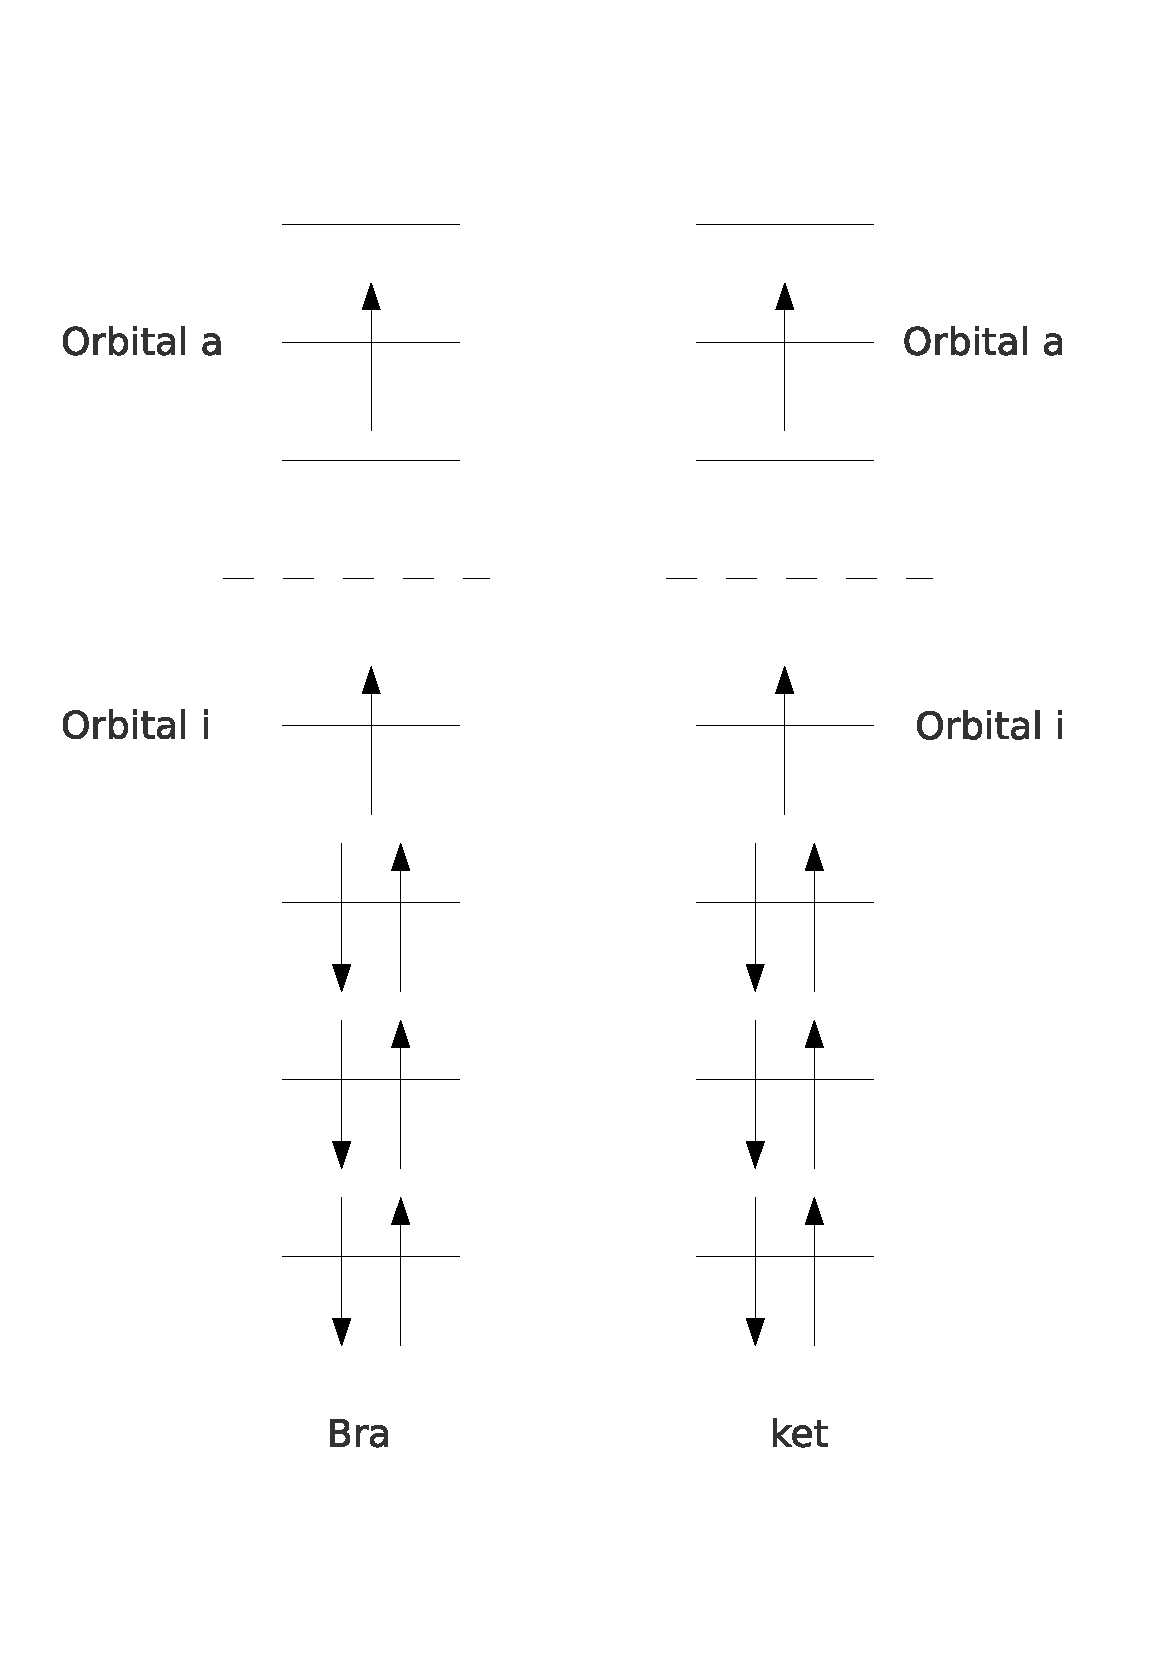
\includegraphics[scale=0.3]{ris1.eps}\label{ris_pic}
\caption{single excitation state}
\end{center}
\end{figure}

By such configuration method, actually we can form $n\times m$ Slater
determinants. Then the trial wave function can be expressed as their
linear combinations:
\begin{equation}
  \label{CISeq:6}
  \Psi = \sum_{i}^{occ}\sum_{a}^{vir}C_{i}^{a}\Phi_{i}^{a}
\end{equation}

Here there are two points should be clarified. Firstly, we note that
in the expression of (\ref{CISeq:6}) the root determinant (ground
state determinant) is not included. Why?

This reason for this is from Brillouin theorem, which has been
demonstrated in the above content. The Brillouin theorem says that the
HF determinant is unable to mix with the single excitation states, so
there's no coupling between them. If we include the HF determinant
into the expression of (\ref{CISeq:6}), the Hamiltonian matrix will be
just like the form below:
\begin{equation}
  \label{CISeq:7}
  \begin{bmatrix}
    \langle\Phi_{HF}|\hat{H}|\Phi_{HF}\rangle & 0  \cdots & \cdots \\
    0 & \langle \Phi_{i}^{a}|\hat{H}|\Phi_{i}^{a} \rangle & \cdots \\
    \cdots & \langle \Phi_{i}^{a}|\hat{H}|\Phi_{i}^{a} \rangle & \cdots \\
  \end{bmatrix}
\end{equation}
Here we can see that the first column and first low are all zero
except the $\langle\Phi_{HF}|\hat{H}|\Phi_{HF}\rangle$, hence it's no
use to put the $\Phi_{HF}$ into the (\ref{CISeq:6}). 

Secondly, we should pay attention to the spin state for each trial
wave function. Actually there are many potential spin states for the
trial wave function, take $H_{2}$ molecule (close shell molecule) as
an example, it's excitation states may be singlet ($S = 0$), or
triplet (S = 1). As what we have said in section \ref{SIC4}, only the
same spin state determinant can mix together so that to form some
trial wave function of $\Psi$:
\begin{align}
  \label{CISeq:8}
\Psi_{single} &= \sum_{i}\sum_{a}C_{i}^{a}\Phi_{single} \nonumber \\
\Psi_{triplet} &= \sum_{i}\sum_{a}C_{i}^{a}\Phi_{triplet}  
\end{align}
That's what I want to say, however; so far we do not take spin into
account so to avoid adding complicity into our consideration.

On the other hand, we note that the forming method for the Slater
determinant can also varied. It can also be unrestricted method, so
the $\alpha$ electrons and $\beta$ electrons are not arranging into
the same spatial orbitals space. However, just as what we have
demonstrated, there are spin contamination situation in the
unrestricted method, so this method is not reliable.

Finally let's take the trial wave function in (\ref{CISeq:6}) into the
Schroedinger equation:
\begin{equation}
  \label{CISeq:9}
  \sum_{i}^{occ}\sum_{a}^{vir}\hat{H}|\Phi_{i}^{a}\rangle C_{i}^{a} = 
E_{CIS} \sum_{i}^{occ}\sum_{a}^{vir}C_{i}^{a}|\Phi_{i}^{a}\rangle
\end{equation}
For short, we abbreviate the $\sum_{i}^{occ}\sum_{a}^{vir}$ as
$\sum_{ia}$. Then we multiply $\Phi_{j}^{b}$ to the above equation, it
becomes: 
\begin{equation}
  \label{CISeq:10}
 \sum_{ia}\langle\Phi_{j}^{b}|\hat{H}|\Phi_{i}^{a}\rangle C_{i}^{a}
 = E_{CIS}\sum_{ia}C_{i}^{a}\delta_{ij}\delta_{ab}
\end{equation}
That's the equation we finally get.

Next, we have to know that how to evaluate the matrix element for the
equation of (\ref{CISeq:10}).


%%%%%%%%%%%%%%%%%%%%%%%%%%%%%%%%%%%%%%%%%%%%%%%%%%%%%
\subsection{Matrix element in CIS equation}
\label{sec:ME_CIS}
%
%
%
%
From the (\ref{CISeq:10}), it's easily to know that there are only
four type of matrix element:
\begin{itemize}
\item $\langle\Phi_{i}^{a}|\hat{H}|\Phi_{i}^{a}\rangle$
\item $\langle\Phi_{i}^{a}|\hat{H}|\Phi_{j}^{a}\rangle$, where $i 
\neq j$
\item $\langle\Phi_{i}^{a}|\hat{H}|\Phi_{i}^{b}\rangle$, where $a 
\neq b$
\item $\langle\Phi_{i}^{a}|\hat{H}|\Phi_{j}^{b}\rangle$, where $i 
\neq j$, $a \neq b$
\end{itemize}

firstly, let's calculate the
$\langle\Phi_{i}^{a}|\hat{H}|\Phi_{i}^{a}\rangle$. For simplicity, we
assume that we are in open shell situation, and the electron on the
orbital $i$ is fired up into the orbital $a$; just as demonstrated in
the picture below:


Based on the HF results, we can have:
\begin{align}
\label{CISeq:11}
  \langle\Phi_{i}^{a}|\hat{H}|\Phi_{i}^{a}\rangle &= \sum_{k\neq
    i}^{occ} \bra{\varphi_{k}}\hat{h}_{1}\ket{\varphi_{k}} - 
\bra{\varphi_{i}}\hat{h}_{1}\ket{\varphi_{i}} + 
\bra{\varphi_{a}}\hat{h}_{1}\ket{\varphi_{a}} \nonumber \\
&+ \sum_{k<l}^{occ}\left\{2[kk|ll] - [kl|kl] \right\} - 
\sum_{k \neq i}^{occ}\left\{2[kk|ii] - [ki|ki] \right\} \nonumber \\
&+ \sum_{k}^{occ}\left\{2[kk|aa] - [ka|ka] \right\} + 
\left\{2[aa|ii] - [ai|ai] \right\}
\end{align}

Firstly we note that in the (\ref{CISeq:11}) it's correspondent to
triplet, where the electrons on the orbital $i$ and orbital $a$ have
the same spin state. On the other hand, if it's the singlet state,
then the exchange term between orbital $i$ and orbital $a$ is
naturally vanished, and the other terms are kept.

Then according to the expression for orbital energy in (\ref{CISeq:3})
and (\ref{CISeq:4}), we can rewrite the whole expression as:
\begin{equation}
  \label{CISeq:12}
    \langle\Phi_{i}^{a}|\hat{H}|\Phi_{i}^{a}\rangle = \Big\{ E_{HF} +
    \varphi_{a} - \varphi_{i}\Big\} + (ii||aa)
\end{equation}
Where the $(ii||aa)$ is abbreviated as:
\begin{equation}
  (ii||aa) = \int dr d r^{'}
  \frac{\varphi_{i}^{*}(r)\varphi_{i}(r)\varphi_{a}^{*}(r^{'})\varphi_{a}(r^{'})
   - \varphi_{i}^{*}(r)\varphi_{a}(r)\varphi_{a}^{*}(r^{'})\varphi_{i}(r^{'})}
  {|r-r^{'}|}
\end{equation}

Secondly, let's go to see the term of
$\langle\Phi_{i}^{a}|\hat{H}|\Phi_{j}^{a}\rangle$ and
$\langle\Phi_{i}^{a}|\hat{H}|\Phi_{i}^{b}\rangle$. For the single
electron energy part, it's easily to show that it's zero; because we
can always find that some orbital in the bra can not find its
counterpart in the ket. For example, in the
$\langle\Phi_{i}^{a}|\hat{H}|\Phi_{j}^{a}\rangle$ if the alpha
electron is fired up from the orbital $i$ to the orbital $a$, then we
still have a beta electron leaving in the orbital $i$. Then it forms
some vacant position in orbital $i$ with alpha spin state. However, we
have the alpha electron in the orbital $i$ in the ket, but its
counterpart in bra is disappeared. 

For the second electron energy part, the same situation holds. In most
of case, no matte how we compose the pair of orbitals, such as
$(ai||ka)$, it's turned out that in the rest of orbitals, there's
always has some orbital that can not find its counterpart so that the
whole integral goes zero. There's only one exception, which is the
integral between occupied-virtual orbital pairs; only this integral
survives. Hence we can finally have:
\begin{align}
  \label{CISeq:13}
  \langle\Phi_{i}^{a}|\hat{H}|\Phi_{j}^{a}\rangle &= (aa||ij)
  \nonumber \\
  \langle\Phi_{i}^{a}|\hat{H}|\Phi_{i}^{b}\rangle &= (ab||ii) 
\end{align}
 
Finally, for the $\langle\Phi_{i}^{a}|\hat{H}|\Phi_{j}^{b}\rangle$,
similarly we only have the $(ij||ab)$ integral does not go zero. So it
can be expressed as:
\begin{equation}
  \label{CISeq:14}
  \langle\Phi_{i}^{a}|\hat{H}|\Phi_{j}^{b}\rangle = (ab||ij)
\end{equation}

All in all, combined the results in the (\ref{CISeq:12}),
(\ref{CISeq:13}) and (\ref{CISeq:14}), we can have the matrix element
in the CIS equation expressed as:
\begin{equation}
  \label{CISeq:15}
  \langle\Phi_{i}^{a}|\hat{H}|\Phi_{j}^{b}\rangle = \Big\{ E_{HF} +
    \varphi_{a} - \varphi_{i}\Big\}\delta_{ij}\delta_{ab} + (ab||ij)
\end{equation}

%%%%%%%%%%%%%%%%%%%%%%%%%%%%%%%%%%%%%%%%%%%%%%%%%
\subsection{CIS Equation}
\label{sec:CIS_solution}
%
%
%
%
%
Now let's take the (\ref{CISeq:15}) into the general form of
(\ref{CISeq:10}), we can have:
\begin{align}
 \label{CISeq:16}
 \sum_{ia}\langle\Phi_{j}^{b}
\left\lbrace (\varphi_{a} - \varphi_{i})\delta_{ij}\delta_{ab} +
(ab||ij)\right\rbrace  C_{i}^{a}
 &=  \sum_{ia}(E_{CIS} -E_{HF})C_{i}^{a}\delta_{ij}\delta_{ab}
\nonumber \\
\left\lbrace
(\varphi_{a} - \varphi_{i})\delta_{ij}\delta_{ab} +
(ab||ij)\right\rbrace  C_{i}^{a} &= \sum_{ia}\omega
C_{i}^{a}\delta_{ij}\delta_{ab} 
\end{align}
Here, $\omega$ is the $E_{CIS} -E_{HF}$ which just characterizes the
excitation energy.

Now we have to enter into the coding procedure, so how can we code
the CIS equation?


%%%%%%%%%%%%%%%%%%%%%%%%%%%%%%%%%%%%%%%%%%%%%%%%%%%%%
\section{The Analytical Gradient for CIS Equation}
%
%
%
%
Now let's step into the gradient of CIS equation. For the expression in
(\ref{CISeq:16}), we have:
\begin{align}
 \label{CIS_gradient:1}
\omega &= \sum_{ai}\sum_{bj}X_{ai}A_{ai,bj}X_{bj} 
\end{align}
Where 
\begin{equation}
 A_{ai,bj} = (\epsilon_{a} - \epsilon_{i})\delta_{ij}\delta_{ab} +
(ai||bj)
\end{equation}
According to the Winger's theorem, for the gradient expression the variational
parameters does not go into it so that we have:
\begin{align}
\label{CIS_gradient:2}
 \omega^{[x]} &= \sum_{ai}\sum_{bj}X_{ai}A^{[x]}_{ai,bj}X_{bj} \nonumber \\
&=   \sum_{ai}\sum_{bj}X_{ai} \left\lbrace( \epsilon^{[x]}_{a} -
\epsilon^{[x]}_{i})\delta_{ij}\delta_{ab} +
(ai||bj)^{[x]}\right\rbrace X_{bj}
\end{align}
Giving by (\ref{CPHF_hf_derivatives_eq:10}), which is:
\begin{align}
  \label{CIS_gradient:3}
  \epsilon^{[x]} &= F_{pp}^{[x]} = H^{x}_{pp} + \sum_{k}^{occ}\left
\{\Pi^{x}_{ppkk} -
    \Pi^{x}_{pkkp} \right\}
  \nonumber \\
  &- S^{x}_{pp}\epsilon_{p} - \sum_{k}^{occ}\sum_{t}^{occ}S^{x}_{kt}
  \left\{ \Pi_{pptk} - \Pi_{ptkp} \right\} \nonumber \\
  &+ \sum_{k}^{occ}\sum_{t}^{vir}U^{x}_{tk}\left\{ 2\Pi_{pptk} -
    \Pi_{ptkp} - \Pi_{pktp} \right\} \nonumber \\
&= F^{x}_{pp} - S^{x}_{pp}\epsilon_{p}
 - \sum_{k}^{occ}\sum_{t}^{occ}S^{x}_{kt}(pp||tk) \nonumber \\
&+2\sum_{k}^{occ}\sum_{t}^{vir}U^{x}_{tk}(pp||tk) 
\end{align}
Where the $F^{x}_{pp} $ is given as:
\begin{equation}
 \label{CIS_gradient:10}
F^{x}_{pp} = H^{x}_{pp} + \sum_{k}^{occ}(pp||kk)^{x}
\end{equation}
$p$ is referred to some general orbital.  For the $\epsilon^{[x]}_{a} -
\epsilon^{[x]}_{i}$, given by the above expression it is:
\begin{equation}
 \begin{split}
\epsilon^{[x]}_{a} - \epsilon^{[x]}_{i} &=  (F^{x}_{aa} -
F^{x}_{ii}) +
(S^{x}_{ii}\epsilon_{i} - S^{x}_{aa}\epsilon_{a})  \\
&+\sum_{k}^{occ}\sum_{l}^{occ}S_{kl}^{x}[(ii||lk) -
(aa||lk)] +  2\sum_{k}^{occ}\sum_{c}^{vir}U_{ck}[(aa||ck) - (ii||ck)]
 \end{split}
\label{CIS_gradient:11}
\end{equation}

As for the gradient expression for $(ai||bj)$ in
(\ref{two_electron_MO_INT_gradient_eq:1}), which is:
\begin{align}
 \label{CIS_gradient:4}
(ai||bj)^{[x]} &= (ai|bj)^{[x]} - (ab|ij)^{[x]} \nonumber \\
&= \sum_{t}\left[ 
U_{ta}(ti|bj) +
U_{ti}(at|bj) + 
U_{tb}(ai|tj) + 
U_{tj}(ai|bt)  
\right] + (ai|bj)^{x} \nonumber \\
&-
\sum_{t}\left[ 
U_{ta}(tb|ij) +
U_{tb}(at|ij) + 
U_{ti}(ab|tj) + 
U_{tj}(ab|it)  
\right] - (ab|ij)^{x} 
%\nonumber \\
%&= \sum_{t}\left[ 
%U_{ta}(ti||bj) +
%U_{ti}(at||bj) + 
%U_{tb}(ai||tj) + 
%U_{tj}(ai||bt)  
%\right] + (ai||bj)^{x}
\end{align}
Since in section of \ref{CPHF} we have derived the fact that within HF
framework, for the orbital response matrix of $U$ only $U_{occ, vir}$ and
$U_{vir, occ}$ exist, the $U_{occ,occ}$ and $U_{vir, vir}$ blocks are zero.
Hence we can safely set the $U_{occ,occ}$ and $U_{vir, vir}$ to zero, so the
(\ref{CIS_gradient:4}) can be transformed into:
\begin{equation}
\begin{split}
(ai||bj)^{[x]} &=
\sum_{k}^{occ}\left\{ U_{ka}\left[(ki|bj) - (kb|ij)\right] \right\} +
\sum_{c}^{vir}\left\{ U_{ci}\left[(ac|bj) - (ab|cj)\right] \right\} \nonumber
\\
&+\sum_{k}^{occ}\left\{ U_{kb}\left[(ai|kj)-(ak|ij)\right] \right\} +
\sum_{c}^{vir}\left\{ U_{cj}\left[(ai|bc)  - (ab|ic)\right] \right\} 
\nonumber \\
&+  (ai|bj)^{x} - (ab|ij)^{x}
\end{split}
 \label{CIS_gradient:12}
\end{equation}
Now let's make some analysis. Since in the expression, the summation is over
all the $i,j,a,b$ label, so actually we can see that:
\begin{align}
\sum_{abc}^{vir}\sum_{i}^{occ}(ai|bc)  &= \sum_{abc}^{vir}\sum_{i}^{occ}(ab|ic)
\nonumber \\
\sum_{ijk}^{occ}\sum_{b}^{occ}(ki|bj) &= \sum_{ijk}^{occ}\sum_{b}^{occ}(kb|ij)
 \label{CIS_gradient:13}
\end{align}
In the first term, we only need to make $a\leftrightarrow c$, and in the second
term to make $j \leftrightarrow k$; then we can derive the equality relation. 

Finally the (\ref{CIS_gradient:12}) becomes:
\begin{equation}
 \begin{split}
 (ai||bj)^{[x]} &=
  \sum_{c}^{vir}\left\{ U_{ci}\left[(ac|bj) - (ab|cj)\right] \right\}
+\sum_{k}^{occ}\left\{ U_{kb}\left[(ai|kj)-(ak|ij)\right] \right\}  \nonumber
\\
&+  (ai|bj)^{x} - (ab|ij)^{x} 
 \end{split}
\label{CIS_gradient:14}
\end{equation}

Finally, we can see that the (\ref{CIS_gradient:2}) becomes:
\begin{align}
 \label{CIS_gradient:6}
\omega^{[x]} &= \sum_{ai}\sum_{bj}X_{ai}\Bigg\{\Big[  (F^{x}_{aa} -
F^{x}_{ii}) +
(S^{x}_{ii}\epsilon_{i} - S^{x}_{aa}\epsilon_{a})  \nonumber \\
&+\sum_{k}^{occ}\sum_{l}^{occ}S_{kl}^{x}[(ii||kl) -
(aa||kl)]\Big]\delta_{ij}\delta_{ab} + (ai||bj)^{x} \Bigg\} X_{bj} \nonumber
\\
&+
\sum_{ai}\sum_{bj}X_{ai}\Bigg\{2\delta_{ij}\delta_{ab}\sum_{k}^{occ}\sum_{c}^{
vir}U_{ck}[(aa||ck) - (ii||ck)]\nonumber \\
& +\sum_{c}^{vir}\left\{ U_{ci}\left[(ac|bj) - (ab|cj)\right] \right\}
+\sum_{k}^{occ}\left\{ U_{kb}\left[(ai|kj)-(ak|ij)\right] \right\} \Bigg\}X_{bj}
\end{align}
In the expression of (\ref{CIS_gradient:6}), there both has $U_{occ, vir}$
and $U_{vir, occ}$ blocks, however; we can use the relation defined in
(\ref{overlap_MO_INT_gradient_eq:3}) to eliminate it:
\begin{align}
 \label{CIS_gradient:7}
U_{kb} &= -U_{bk} - S_{bk}^{x}
\end{align}
Then the (\ref{CIS_gradient:6}) becomes:
\begin{align}
 \label{CIS_gradient:7}
\omega^{[x]} &= \sum_{ai}\sum_{bj}X_{ai}\Bigg\{\Big[  (F^{x}_{aa} -
F^{x}_{ii}) +
(S^{x}_{ii}\epsilon_{i} - S^{x}_{aa}\epsilon_{a})  \nonumber \\
&+\sum_{k}^{occ}\sum_{l}^{occ}S_{kl}^{x}[(ii||kl) -
(aa||kl)]\Big]\delta_{ij}\delta_{ab} \nonumber
\\ 
& -\sum_{k}^{occ}\left\{S^{x}_{bk}\left[(ai|kj)-(ak|ij)\right] \right\} +
(ai||bj)^{x} \Bigg\} X_{bj} 
\nonumber \\
&+
\sum_{ai}\sum_{bj}X_{ai}\Bigg\{2\delta_{ij}\delta_{ab}\sum_{k}^{occ}\sum_{c}^{
vir}U_{ck}[(aa||ck) - (ii||ck)]\nonumber \\
&+\sum_{c}^{vir}\left\{ U_{ci}\left[(ac|bj) - (ab|cj)\right] \right\}
-\sum_{k}^{occ}\left\{ U_{bk}\left[(ai|kj)-(ak|ij)\right] \right\} \Bigg\}X_{bj}
\end{align} 

Now we can abbreviate the term related to $U$ matrix as:
\begin{align} 
\label{CIS_gradient:8}
 Y_{ck} &= 2\sum_{ai}\sum_{bj}X_{ai}X_{bj}
\delta_{ij}\delta_{ab}[(aa||ck) - (ii||ck)]\nonumber \\
&+\sum_{ab}\sum_{j}X_{ak}X_{bj}\left\{\left[(ac|bj)
- (ab|cj)\right] \right\} \nonumber \\
&-\sum_{a}\sum_{ij}X_{ai}X_{cj}\left\{
\left[(ai|kj)-(ak|ij)\right] \right\} 
\end{align}

Then (\ref{CIS_gradient:7}) becomes:
\begin{align}
 \label{CIS_gradient:9}
\omega^{[x]} &=  \sum_{ai}\sum_{bj}X_{ai}\Bigg\{\Big[  (F^{x}_{aa} -
F^{x}_{ii}) +
(S^{x}_{ii}\epsilon_{i} - S^{x}_{aa}\epsilon_{a})  \nonumber \\
&+\sum_{k}^{occ}\sum_{l}^{occ}S_{kl}^{x}[(ii||kl) -
(aa||kl)]\Big]\delta_{ij}\delta_{ab} \nonumber
\\ 
& -\sum_{k}^{occ}\left\{S^{x}_{bk}\left[(ai|kj)-(ak|ij)\right] \right\} +
(ai||bj)^{x} \Bigg\} X_{bj} 
\nonumber \\
&+\sum_{c}^{vir}\sum_{k}^{occ}U_{ck}Y_{ck}
\end{align}

%%%%%%%%%%%%%%%%%%%%%%%%%%%%%%%%%%%%%%%%%%%%%%%%%%%%%
\subsection{Z-Vector Method}
%
%
%
Now the issue inside the (\ref{CIS_gradient:9}) is that we have to solve the
$U$ matrix so that to get the explicit derivative expression. By using the CPHF
equation, which is shown in (\ref{CPHF_hf_derivatives_eq:17}) and
(\ref{CPHF_hf_derivatives_eq:18}), we generally have:
\begin{equation}
 \label{Zvector_CIS_eq:1}
AU^{a} = B^{a}\Leftrightarrow \sum_{jb}A_{ij, ab}U^{a}_{bj} =
B^{a}_{ia} \Rightarrow AU = B
\end{equation}
Where matrix of $A$ is $(occ\times vir)^{2}$ dimension, the U and $B$ are both
$occ\times vir$ dimension.

For the (\ref{Zvector_CIS_eq:1}), it can be further expressed as:
\begin{equation}
 \label{Zvector_CIS_eq:2}
U = A^{-1}B
\end{equation}
Now let's make a direct product between $U$ matrix and the $Y$ matrix defined
in (\ref{CIS_gradient:9}), combined with (\ref{Zvector_CIS_eq:2}), it's (for
matching with the label in \ref{CIS_gradient:8}, we use the label of $c,k$ etc.
rather than $b,j$ etc.):
\begin{align}
  \label{Zvector_CIS_eq:3}
\sum_{c}^{vir}\sum_{k}^{occ}U_{ck}Y_{ck} &=
\sum_{c}^{vir}\sum_{d}^{vir}\sum_{k}^{occ}\sum_{l}^{occ}A_{kl,cd}^{-1}B^{a}_{ld}
Y_{ck} \Rightarrow \nonumber \\
\sum_{c}^{vir}\sum_{k}^{occ}U_{ck}Y_{ck} &=
\sum_{d}^{vir}\sum_{l}^{occ}Z_{dl}B^{a}_{ld}
\end{align}
Where the vector of $Z$ is given by:
\begin{equation}
 \label{Zvector_CIS_eq:4}
Z_{dl} = \sum_{c}^{vir}\sum_{k}^{occ}A_{kl,cd}^{-1}Y_{ck} \Rightarrow
\sum_{d}^{vir}\sum_{l}^{occ}A_{kl,cd}Z_{dl} = Y_{ck}
\end{equation}

The new vector of $Z$, compared with the MO rotation matrix of $U$, only has
the dimension of $occ*vir$ for all the perturbations; that means; the $Z$ vector 
can be solved only once and used for all the $3\times N$ atoms gradient
calculation. That's the advantages that why we solve the Z-vector rather than
the rotation matrix of $U$. 

Now let's expand the (\ref{Zvector_CIS_eq:4}) into more detailed way:
\begin{equation}
 \begin{split}
&\sum_{l}^{occ}\sum_{d}^{vir}\left\lbrace   \left(\epsilon_{c} -
\epsilon_{k}\right)\delta_{kl}\delta_{cd} + \left[
2(kc|dl) -(kd|lc) - (kl|dc) \right] \right\rbrace Z_{dl} =  \\
&2\sum_{ai}\sum_{bj}X_{ai}X_{bj}
\delta_{ij}\delta_{ab}[(aa||ck) - (ii||ck)] 
+\sum_{ab}\sum_{j}X_{ak}X_{bj}\left\{\left[(ac|bj)
- (ab|cj)\right] \right\}  \\
&-\sum_{a}\sum_{ij}X_{ai}X_{cj}\left\{
\left[(ai|kj)-(ak|ij)\right] \right\}
 \end{split}
 \label{Zvector_CIS_eq:5}
\end{equation}

After getting the vector of $Z$, then we can get the gradient expression for CIS equation.

%%%%%%%%%%%%%%%%%%%%%%%%%%%%%%%%%%%%%%%%%%%%%%%%%%%%%

%%% Local Variables: 
%%% mode: latex
%%% TeX-master: "../../main"
%%% End: 



%%
% created around Jan. 29th, 2009
%
%
%
%
\chapter{Molecular Vibration}
%
%
%
%
%%%%%%%%%%%%%%%%%%%%%%%%%%%%%%%%%%%%%%%%%%%%%%%%%%%%%%%%%%%%%%%%%%%%%
\section{Introduction}
%
%
%
%%%%%%%%%%%%%%%%%%%%%%%%%%%%%%%%%%%%%%%%%%%%%%%%%%%%%%%%%%%%%%%%%%%%%





%%% Local Variables: 
%%% mode: latex
%%% TeX-master: "../../main"
%%% End: 

%%
%
%
%
%
%
\chapter{Perturbation Treatment in Molecular Quantum Mechanics}
%
%
%
%
%%%%%%%%%%%%%%%%%%%%%%%%%%%%%%%%%%%%%%%%%%%%%%%%%%%%%%%%%%%%%%%%%%%%%%%%%%%%%%%%%%%%%%%%%%%%%%%%%
\section{Introduction}
%
% what does the perturbation treatment do in the quantum chemistry
%
%
In quantum chemistry, the perturbation treatment is usually employed
to tackle with the weak interactions in the molecular systems. Such
weak interaction can be in variety kinds, such as the vibration of
atom skeleton, or the magnetic susceptibility and
shielding\cite{stevens:550}; or even the time dependent external
field change etc. In general, such physical quantity are very small
so that it's suitable to be the perturbation operator, and the
perturbation treatment can usually yield good results.

%%%%%%%%%%%%%%%%%%%%%%%%%%%%%%%%%%%%%%%%%%%%%%%%%%%%%%%%%%%%%%%%%%%%%%%%%%%%%%%%%%%%%%%%%%%%%%%%%
\section{The perturbed Hatree-Fock equation in differential form}
%
%  1  start from the Fock equation, the orbital is involved. we
%     do not consider its expansion
%  2  perturbation expansion for the orbital and the orbital energy
%
%
Firstly let's derive the general procedure for the perturbation
treatment in the Hatree-Fock framework\cite{PhysRev.118.167,
Peng_H_W, RevModPhys.32.455}.

As what has been shown in the Hatree-Fock chapter, the general
Hatree-Fock equation in molecular orbital form can be expressed as:
\begin{multline}\label{PTIMQMeq:1}
\hat{H}_{1}(1)\varphi_{i}(1) + \sum_{j}\left[
\left\{\int\varphi^{*}_{j}(2)\varphi_{j}(2)d\tau(2)\frac{1}{r_{12}}\right\}\varphi_{i}(1)
\right] \\
 -
\sum_{j}\left[
\left\{\int\varphi^{*}_{j}(2)\varphi_{i}(2)d\tau(2)\frac{1}{r_{12}}\right\}\varphi_{j}(1)
\right] \\
 = \epsilon_{i}\varphi_{i}(1)
\end{multline}
Here the $j$ goes over all the occupied orbitals. Here for
simplicity we only consider the differential form of Hatree-Fock
equation, the involvement of basis sets are left for the future.

Suggest there's some perturbation in the Fock operator, and it's
assumed to be the one electron operator-where such assumption can
satisfy most of the perturbation cases. In the presence of the
perturbed operator, the molecular orbitals and the its energy levels
will make corresponding change; we can express such changes in
progressive way:
\begin{align}\label{PTIMQMeq:2}
\varphi_{i} &= \varphi^{(0)}_{i} + \lambda\varphi^{(1)}_{i} +
\lambda^{2}\varphi^{(2)}_{i} + \cdots \nonumber \\
\epsilon_{i} &= \epsilon^{(0)}_{i} + \lambda\epsilon^{(1)}_{i} +
\lambda^{2}\epsilon^{(2)}_{i} + \cdots
\end{align}
The new Fock operator can be expressed as:
\begin{equation}\label{PTIMQMeq:3}
\hat{F}^{'} = \hat{F} + \lambda \hat{V}
\end{equation}
Now we go to see how to get the perturbed HF equations.

%%%%%%%%%%%%%%%%%%%%%%%%%%%%%%%%%%%%%%%%%%%%%%%%%%%%%%%%%%%%%%%%%%%%%%%%%%%%%%%%%%%%%%%%%%%%%%%%%
\subsection{First order Hatree Fock perturbed equation}
%
%   to get the first order Fock equation
%
By taking the (\ref{PTIMQMeq:2}) and (\ref{PTIMQMeq:3}) into the
original Hatree-Fock equation (\ref{PTIMQMeq:1}), then by gathering
the terms with same power of $\lambda$, we can get a series of
perturbation equations. The equation scales with $\lambda^{0}$ is:
\begin{equation}\label{PTIMQMeq:4}
\hat{F}\varphi^{(0)}_{i} = \epsilon^{(0)}_{i}\varphi^{(0)}_{i}
\end{equation}
That's the equation for the zero order approximation.

By gathering the terms related to the $\lambda$, we can get the
first order approximation:
\begin{multline}\label{PTIMQMeq:6}
\hat{H}_{1}\varphi^{(1)}_{i} + \hat{V}\varphi^{(0)}_{i} \\
+\sum_{j}\Bigg\{
\int\varphi^{*(0)}_{j}\varphi^{(1)}_{j}d\tau\frac{1}{r_{12}}\varphi^{(0)}_{i}
+
\int\varphi^{*(1)}_{j}\varphi^{(0)}_{j}d\tau\frac{1}{r_{12}}\varphi^{(0)}_{i}
+
\int\varphi^{*(0)}_{j}\varphi^{(0)}_{j}d\tau\frac{1}{r_{12}}\varphi^{(1)}_{i}
\Bigg\} \\
-\sum_{j}\Bigg\{
\int\varphi^{*(0)}_{j}\varphi^{(1)}_{i}d\tau\frac{1}{r_{12}}\varphi^{(0)}_{j}
+
\int\varphi^{*(1)}_{j}\varphi^{(0)}_{i}d\tau\frac{1}{r_{12}}\varphi^{(0)}_{j}
+
\int\varphi^{*(0)}_{j}\varphi^{(0)}_{i}d\tau\frac{1}{r_{12}}\varphi^{(1)}_{j}
\Bigg\} \\
=\epsilon^{(0)}_{i}\varphi^{(1)}_{i} +
\epsilon^{(1)}_{i}\varphi^{(0)}_{i}
\end{multline}
However, we can arrange the above equation into the more convenient
form:
\begin{multline}\label{PTIMQMeq:5}
\hat{F}\varphi^{(1)}_{i} - \epsilon^{(0)}_{i}\varphi^{(1)}_{i} =
\epsilon^{(1)}_{i}\varphi^{(0)}_{i} - \hat{V}\varphi^{(0)}_{i} \\
-\sum_{j}\Bigg\{
\int\varphi^{*(0)}_{j}\varphi^{(1)}_{j}d\tau\frac{1}{r_{12}}\varphi^{(0)}_{i}
+
\int\varphi^{*(1)}_{j}\varphi^{(0)}_{j}d\tau\frac{1}{r_{12}}\varphi^{(0)}_{i}
\\
-
\int\varphi^{*(1)}_{j}\varphi^{(0)}_{i}d\tau\frac{1}{r_{12}}\varphi^{(0)}_{j}
-
\int\varphi^{*(0)}_{j}\varphi^{(0)}_{i}d\tau\frac{1}{r_{12}}\varphi^{(1)}_{j}
\Bigg\}
\end{multline}
Here the items related to the $\varphi^{(1)}_{i}$ are put to the
left of the equation, and the others related to the
$\varphi^{(0)}_{i}$ are put to the right side. Furthermore the
$\hat{F}\varphi^{(1)}_{i}$ is:
\begin{multline}\label{PTIMQMeq:18}
\hat{F}\varphi^{(1)}_{i} = \hat{H}_{1}\varphi^{(1)}_{i} +
\sum_{j}\left[
\left\{\int\varphi^{*(0)}_{j}\varphi^{(0)}_{j}d\tau\frac{1}{r_{12}}\right\}
\varphi^{(1)}_{i}
\right. \\
 -
\left.
\left\{\int\varphi^{*(0)}_{j}\varphi^{(1)}_{i}d\tau\frac{1}{r_{12}}\right\}
\varphi^{(0)}_{j} \right]
\end{multline}
Compared with the (\ref{PTIMQMeq:1}) we have omitted all the
explicit electron labels for simplicity. Besides, the higher order
equations can be obtained in a like manner, but here we concentrate
on the discussion of first order perturbation equation.

By multiply the equation with $\varphi^{*(0)}_{i}$, we can get the
expression for the first order energy for the molecular orbitals:
\begin{multline}\label{PTIMQMeq:13}
\epsilon^{(1)}_{i}=
\int\varphi^{*(0)}_{i}\hat{V}\varphi^{(0)}_{i}d\tau + \\
\sum_{j}\Bigg\{
\int\varphi^{*(0)}_{j}\varphi^{(1)}_{j}d\tau\frac{1}{r_{12}}
    \varphi^{*(0)}_{i}\varphi^{(0)}_{i}d\tau +
\int\varphi^{*(1)}_{j}\varphi^{(0)}_{j}d\tau\frac{1}{r_{12}}
    \varphi^{*(0)}_{i}\varphi^{(0)}_{i}d\tau
\\
-
\int\varphi^{*(1)}_{j}\varphi^{(0)}_{i}d\tau\frac{1}{r_{12}}
    \varphi^{*(0)}_{i}\varphi^{(0)}_{j}d\tau
-
\int\varphi^{*(0)}_{j}\varphi^{(0)}_{i}d\tau\frac{1}{r_{12}}
    \varphi^{*(0)}_{i}\varphi^{(1)}_{j}d\tau
\Bigg\}
\end{multline}


%%%%%%%%%%%%%%%%%%%%%%%%%%%%%%%%%%%%%%%%%%%%%%%%%%%%%%%%%%%%%%%%%%%%%%%%%%%%%%%%%%%%%%%%%%%%%%%%%
\subsection{Relations between the perturbed molecular
orbitals}\label{PTIMQM:1}
%
%   consideration about the relations between the wave functions
%
Next we will consider the relations between the $\varphi^{(0)}_{i}$,
$\varphi^{(1)}_{i}$ etc. For the $\varphi^{(0)}_{i}$, it's known
that it equals to the unperturbed HF orbitals:
\begin{align}\label{}
\varphi^{(0)}_{i} &= \varphi_{i}  \nonumber \\
\epsilon^{(0)}_{i} &= \epsilon_{i}
\end{align}
Furthermore, these orbitals can be safely assumed to be orthogonal
with each other:
\begin{equation}\label{}
\int \varphi^{*(0)}_{i}\varphi^{(0)}_{j} d\tau = \delta_{ij}
\end{equation}

For the $\varphi^{(0)}_{i}$, $\varphi^{(1)}_{i}$, we can prove that
they are orthogonal with each other:
\begin{equation}\label{PTIMQMeq:19}
\int \varphi^{*(0)}_{i}\varphi^{(1)}_{i} d\tau = 0
\end{equation}
Such relation can be obtained via the normalization condition of the
$\varphi_{i}$. Suggest that the $\varphi_{i}$ is approximated at the
first order, then we have:
\begin{align}\label{}
\int \varphi^{*}_{i}\varphi_{i} d\tau &= 1  \Rightarrow \nonumber \\
\int \varphi^{*(0)}_{i}\varphi^{(1)}_{i} d\tau  + \int
\varphi^{*(1)}_{i}\varphi^{(0)}_{i} d\tau &= 0
\end{align}
Since that we have:
\begin{equation}\label{}
\int \varphi^{*(0)}_{i}\varphi^{(1)}_{i} d\tau  = \left\{\int
\varphi^{*(1)}_{i}\varphi^{(0)}_{i} d\tau\right\}^{*}
\end{equation}
Then the integral should be some imaginary number so that it can be
set to zero without hurting the generality. Therefore the
orthogonality condition has been proved.

For the $\varphi^{(0)}_{i}$, $\varphi^{(1)}_{k}$ where $k\neq i$, we
can have the relation that:
\begin{equation}\label{PTIMQMeq:9}
\int \varphi^{*(0)}_{i}\varphi^{(1)}_{k} d\tau  + \int
\varphi^{*(1)}_{i}\varphi^{(0)}_{k} d\tau = 0
\end{equation}
This can be achieved through the (\ref{PTIMQMeq:5}). If we take
complex conjugation of the equation in (\ref{PTIMQMeq:5}) and
multiply the $\varphi^{(0)}_{k}$ then to integrate, we can get some
equation:
\begin{multline}\label{PTIMQMeq:7}
\langle\varphi^{(1)}_{i}|\hat{F}|\varphi^{(0)}_{k}\rangle -
\epsilon^{(0)}_{i}\langle\varphi^{(1)}_{i}|\varphi^{(0)}_{k}\rangle
=
- \langle\varphi^{(0)}_{i}|\hat{V}|\varphi^{(0)}_{k}\rangle \\
-\sum_{j}\Bigg\{
\left(\varphi^{(1)}_{j}\varphi^{(0)}_{j}|\varphi^{(0)}_{i}\varphi^{(0)}_{k}\right)
+
\left(\varphi^{(0)}_{j}\varphi^{(1)}_{j}|\varphi^{(0)}_{i}\varphi^{(0)}_{k}\right)
\\
-
\left(\varphi^{(0)}_{i}\varphi^{(1)}_{j}|\varphi^{(0)}_{j}\varphi^{(0)}_{k}\right)
-
\left(\varphi^{(0)}_{i}\varphi^{(0)}_{j}|\varphi^{(1)}_{j}\varphi^{(0)}_{k}\right)
\Bigg\}
\end{multline}
Here we use the Dirac notion to express the single electron
integral, on the other hand the double electron integral is shorten
as:
\begin{equation}\label{}
\left(\varphi^{(1)}_{j}\varphi^{(0)}_{j}|\varphi^{(0)}_{i}\varphi^{(0)}_{k}\right)
= \int \int
\varphi^{*(1)}_{j}(1)\varphi^{(0)}_{j}(1)\frac{1}{r_{12}}
\varphi^{*(0)}_{i}(2)\varphi^{(0)}_{k}(2)d\tau_{1}d\tau_{2}
\end{equation}
Such abbreviation is to make the derivation as clear as possible.

On the other hand, if the equation in (\ref{PTIMQMeq:5}) in on
$\varphi^{(1)}_{k}$ and we multiply the $\varphi^{*(0)}_{i}$ then to
make integration, we can get similar equation with
(\ref{PTIMQMeq:7}):
\begin{multline}\label{PTIMQMeq:8}
\langle\varphi^{(0)}_{i}|\hat{F}|\varphi^{(1)}_{k}\rangle -
\epsilon^{(0)}_{k}\langle\varphi^{(0)}_{i}|\varphi^{(1)}_{k}\rangle
=
- \langle\varphi^{(0)}_{i}|\hat{V}|\varphi^{(0)}_{k}\rangle \\
-\sum_{j}\Bigg\{
\left(\varphi^{(0)}_{j}\varphi^{(1)}_{j}|\varphi^{(0)}_{i}\varphi^{(0)}_{k}\right)
+
\left(\varphi^{(1)}_{j}\varphi^{(0)}_{j}|\varphi^{(0)}_{i}\varphi^{(0)}_{k}\right)
\\
-
\left(\varphi^{(1)}_{j}\varphi^{(0)}_{k}|\varphi^{(0)}_{i}\varphi^{(0)}_{j}\right)
-
\left(\varphi^{(0)}_{j}\varphi^{(0)}_{k}|\varphi^{(0)}_{i}\varphi^{(1)}_{j}\right)
\Bigg\}
\end{multline}
Hence it's easy to see that the right part of (\ref{PTIMQMeq:7}) is
same with the right side of (\ref{PTIMQMeq:8}), therefore we have:
\begin{align}\label{PTIMQMeq:27}
\langle\varphi^{(0)}_{i}|\hat{F}|\varphi^{(1)}_{k}\rangle -
\epsilon^{(0)}_{k}\langle\varphi^{(0)}_{i}|\varphi^{(1)}_{k}\rangle
&=\langle\varphi^{(1)}_{i}|\hat{F}|\varphi^{(0)}_{k}\rangle -
\epsilon^{(0)}_{i}\langle\varphi^{(1)}_{i}|\varphi^{(0)}_{k}\rangle
\nonumber \\
(\epsilon^{(0)}_{i}-\epsilon^{(0)}_{k})
\langle\varphi^{(0)}_{i}|\varphi^{(1)}_{k}\rangle &=
(\epsilon^{(0)}_{k}-\epsilon^{(0)}_{i})
\langle\varphi^{(1)}_{i}|\varphi^{(0)}_{k}\rangle
\end{align}
Then we can get the conclusion in the (\ref{PTIMQMeq:9}).

Nevertheless, in such derivation if the energy level is degenerated
(which means that we have $\epsilon^{(0)}_{k}=\epsilon^{(0)}_{i}$
for the $k\neq i$); we can not get the conclusion of
(\ref{PTIMQMeq:9}) directly from the (\ref{PTIMQMeq:27}). However,
there is another way to derive the relation shown in the
(\ref{PTIMQMeq:9}), which is similar to the way we got the relation
in (\ref{PTIMQMeq:19}).

Once again we use the normalization condition for the $\varphi_{i}$.
Suggest that the $\varphi_{i}$ is approximated at the first order,
then we have:
\begin{align}\label{}
\int \varphi^{*}_{i}\varphi_{k} d\tau = 0 \quad  i\neq k &
\Rightarrow \nonumber \\
\int (\varphi^{*(0)}_{i} + \lambda\varphi^{*(1)}_{i})
(\varphi^{(0)}_{k} + \lambda\varphi^{(1)}_{k}) d\tau &=0 \nonumber
\\
\int\varphi^{*(0)}_{i}\varphi^{(0)}_{k} d\tau  + \lambda(\int
\varphi^{*(0)}_{i}\varphi^{(1)}_{k} d\tau + \int
\varphi^{*(1)}_{i}\varphi^{(0)}_{k} d\tau) + O(\lambda^{2}) &= 0
\end{align}

Because the unperturbed orbitals are orthogonal with each other,
thus $\int\varphi^{*(0)}_{i}\varphi^{(0)}_{k} d\tau = 0$.
Furthermore, since $\lambda$ is some arbitrary number, therefore it
requires that:
\begin{equation}
\int \varphi^{*(0)}_{i}\varphi^{(1)}_{k} d\tau + \int
\varphi^{*(1)}_{i}\varphi^{(0)}_{k} d\tau = 0
\end{equation}
This is just the conclusion in the (\ref{PTIMQMeq:9}). We note that
this proof does not refer to the energy degeneracy so that the
conclusion in the (\ref{PTIMQMeq:9}) is holding in all cases.

All in all, we can get the relations between the first order
correlated orbital of $\varphi^{(1)}_{i}$ and the unperturbed
orbital of $\varphi^{(0)}_{j}$:
\begin{equation}\label{}
\int \varphi^{*(0)}_{i}\varphi^{(1)}_{j} d\tau + \int
\varphi^{*(1)}_{i}\varphi^{(0)}_{j} d\tau = 0
\end{equation}
Here the label of $i$ and $j$ can be any kind of orbitals.

%%%%%%%%%%%%%%%%%%%%%%%%%%%%%%%%%%%%%%%%%%%%%%%%%%%%%%%%%%%%%%%%%%%%%%%%%%%%%%%%%%%%%%%%%%%%%%%%%
\subsection{The first order total energy expression}
%
% consider the total energy expression under the perturbation framework
%
Next we switch to the total energy derivation. According to the
results we have gotten in the HF chapter, the total energy for an
arbitrary $n$ electrons system is:
\begin{multline}\label{PTIMQMeq:10}
E =
\sum_{i}^{n}\langle\varphi_{i}(1)|\hat{H}_{1}(1)|\varphi_{i}(1)\rangle
+
\\
\frac{1}{2}\sum_{i}\sum_{j} \left\{
\int\int\varphi^{*}_{i}(1)\varphi_{i}(1)\frac{1}{r_{12}}
\varphi^{*}_{j}(2)\varphi_{j}(2)d\tau_{1}d\tau_{2}- \right. \\
\left.
\int\int\varphi^{*}_{i}(1)\varphi_{j}(1)\frac{1}{r_{12}}
\varphi^{*}_{j}(2)\varphi_{i}(2)d\tau_{1}d\tau_{2} \right\}
\end{multline}

Similarly, the total energy can be also expanded according to the
order of $\lambda$:
\begin{equation}\label{}
E = E^{(0)} + \lambda E^{(1)} + \lambda^{2}E^{(2)} + \cdots
\end{equation}
Now by taking the expansion for $\varphi$ defined in
(\ref{PTIMQMeq:2}) as well as the total energy expansion into the
(\ref{PTIMQMeq:10}), we can get the perturbation equations for $E$.

The zero order approximation for the total energy equation is:
\begin{multline}\label{PTIMQMeq:11}
E^{(0)} =
\sum_{i}^{n}\langle\varphi^{(0)}_{i}|\hat{H}_{1}|\varphi^{(0)}_{i}\rangle
+
\\
\frac{1}{2}\sum_{i}\sum_{j} \left\{
\int\int\varphi^{*(0)}_{i}\varphi^{(0)}_{i}\frac{1}{r_{12}}
\varphi^{*(0)}_{j}\varphi^{(0)}_{j}d\tau_{1}d\tau_{2}- \right. \\
\left. \int\int\varphi^{*(0)}_{i}\varphi^{(0)}_{j}\frac{1}{r_{12}}
\varphi^{*(0)}_{j}\varphi^{(0)}_{i}d\tau_{1}d\tau_{2} \right\}
\end{multline}
On the other hand, by using the orbital energy we can express it as:
\begin{multline}\label{PTIMQMeq:12}
E^{(0)} = \sum_{i}^{n}\epsilon_{i}^{(0)} -
\frac{1}{2}\sum_{i}\sum_{j} \left\{
\int\int\varphi^{*(0)}_{i}\varphi^{(0)}_{i}\frac{1}{r_{12}}
\varphi^{*(0)}_{j}\varphi^{(0)}_{j}d\tau_{1}d\tau_{2}- \right. \\
\left. \int\int\varphi^{*(0)}_{i}\varphi^{(0)}_{j}\frac{1}{r_{12}}
\varphi^{*(0)}_{j}\varphi^{(0)}_{i}d\tau_{1}d\tau_{2} \right\}
\end{multline}

For the first order approximation, it scales with $\lambda$ and we
can express this term as:
\begin{multline}\label{PTIMQMeq:14}
E^{(1)} =\sum_{i}^{n}
\Bigg\{\langle\varphi^{(1)}_{i}|\hat{H}_{1}|\varphi^{(0)}_{i}\rangle
      +\langle\varphi^{(0)}_{i}|\hat{H}_{1}|\varphi^{(1)}_{i}\rangle +
       \langle\varphi^{(0)}_{i}|\hat{V}|\varphi^{(0)}_{i}\rangle\Bigg\}
\\
+\frac{1}{2}\sum_{i}\sum_{j}\Bigg\{
\left(\varphi^{(1)}_{i}\varphi^{(0)}_{i}|\varphi^{(0)}_{j}\varphi^{(0)}_{j}\right)
+
\left(\varphi^{(0)}_{i}\varphi^{(1)}_{i}|\varphi^{(0)}_{j}\varphi^{(0)}_{j}\right)
\\
+
\left(\varphi^{(0)}_{i}\varphi^{(0)}_{i}|\varphi^{(1)}_{j}\varphi^{(0)}_{j}\right)
+
\left(\varphi^{(0)}_{i}\varphi^{(0)}_{i}|\varphi^{(0)}_{j}\varphi^{(1)}_{j}\right)
\Bigg\} \\
-\frac{1}{2}\sum_{i}\sum_{j}\Bigg\{
\left(\varphi^{(1)}_{i}\varphi^{(0)}_{j}|\varphi^{(0)}_{j}\varphi^{(0)}_{i}\right)
+
\left(\varphi^{(0)}_{i}\varphi^{(1)}_{j}|\varphi^{(0)}_{j}\varphi^{(0)}_{i}\right)
\\
+
\left(\varphi^{(0)}_{i}\varphi^{(0)}_{j}|\varphi^{(1)}_{j}\varphi^{(0)}_{i}\right)
+
\left(\varphi^{(0)}_{i}\varphi^{(0)}_{j}|\varphi^{(0)}_{j}\varphi^{(1)}_{i}\right)
\Bigg\} \\
\end{multline}

This expression is too much complicated. Therefore, by using the
relation we have got before, we try to reduce it into some simpler
form. Firstly, from the (\ref{PTIMQMeq:13}) we can see that the two
electrons integral can be expressed as:
\begin{multline}\label{PTIMQMeq:16}
\sum_{i}\sum_{j}\Bigg\{
\left(\varphi^{(0)}_{j}\varphi^{(1)}_{j}|\varphi^{(0)}_{i}\varphi^{(0)}_{i}\right)
+
\left(\varphi^{(1)}_{j}\varphi^{(0)}_{j}|\varphi^{(0)}_{i}\varphi^{(0)}_{i}\right)
\\
-
\left(\varphi^{(1)}_{j}\varphi^{(0)}_{i}|\varphi^{(0)}_{i}\varphi^{(0)}_{j}\right)
-
\left(\varphi^{(0)}_{j}\varphi^{(0)}_{i}|\varphi^{(0)}_{i}\varphi^{(1)}_{j}\right)
\Bigg\} \\
= \sum_{i}\Bigg\{\epsilon^{(1)}_{i} -
\langle\varphi^{(0)}_{i}|\hat{V}|\varphi^{(0)}_{i}\rangle\Bigg\}
\end{multline}
By exchanging the label of $i$ and $j$ on the right side of the
above equation (such operation will change nothing), we can get:
\begin{multline}\label{PTIMQMeq:15}
\sum_{i}\sum_{j}\Bigg\{
\left(\varphi^{(0)}_{i}\varphi^{(1)}_{i}|\varphi^{(0)}_{j}\varphi^{(0)}_{j}\right)
+
\left(\varphi^{(1)}_{i}\varphi^{(0)}_{i}|\varphi^{(0)}_{j}\varphi^{(0)}_{j}\right)
\\
-
\left(\varphi^{(1)}_{i}\varphi^{(0)}_{j}|\varphi^{(0)}_{j}\varphi^{(0)}_{i}\right)
-
\left(\varphi^{(0)}_{i}\varphi^{(0)}_{j}|\varphi^{(0)}_{j}\varphi^{(1)}_{i}\right)
\Bigg\} \\
= \sum_{i}\Bigg\{\epsilon^{(1)}_{i} -
\langle\varphi^{(0)}_{i}|\hat{V}|\varphi^{(0)}_{i}\rangle\Bigg\}
\end{multline}
That's half part of the two electron integrals in the
(\ref{PTIMQMeq:14}).

On the other hand, in the (\ref{PTIMQMeq:16}) we can exchange the
electron label in the two electron integrals, that is to make:
\begin{equation}\label{}
(ii|jj) \Rightarrow (jj|ii)
\end{equation}
Certainly such operation will not change the integrals. Thus we can
transform the (\ref{PTIMQMeq:16}) into:
\begin{multline}\label{PTIMQMeq:17}
\sum_{i}\sum_{j}\Bigg\{
\left(\varphi^{(0)}_{i}\varphi^{(0)}_{i}|\varphi^{(0)}_{j}\varphi^{(1)}_{j}\right)
+
\left(\varphi^{(0)}_{i}\varphi^{(0)}_{i}|\varphi^{(1)}_{j}\varphi^{(0)}_{j}\right)
\\
-
\left(\varphi^{(0)}_{i}\varphi^{(0)}_{j}|\varphi^{(1)}_{j}\varphi^{(0)}_{i}\right)
-
\left(\varphi^{(0)}_{i}\varphi^{(1)}_{j}|\varphi^{(0)}_{j}\varphi^{(0)}_{i}\right)
\Bigg\} \\
= \sum_{i}\Bigg\{\epsilon^{(1)}_{i} -
\langle\varphi^{(0)}_{i}|\hat{V}|\varphi^{(0)}_{i}\rangle\Bigg\}
\end{multline}
Now it can see this is the other half part of the two electron
integrals in the (\ref{PTIMQMeq:14}).

All in all, by the expression in (\ref{PTIMQMeq:15}) and
(\ref{PTIMQMeq:17}) the (\ref{PTIMQMeq:14}) can be transformed into:
\begin{equation}\label{PTIMQMeq:22}
E^{(1)} =\sum_{i}^{n} \left\{\epsilon^{(1)}_{i} +
\langle\varphi^{(1)}_{i}|\hat{H}_{1}|\varphi^{(0)}_{i}\rangle
      +\langle\varphi^{(0)}_{i}|\hat{H}_{1}|\varphi^{(1)}_{i}\rangle\right\}
\end{equation}

so far we have gotten some simpler expression for the $E^{(1)}$,
however; the concrete expression for the $\epsilon^{(1)}_{i}$ is not
known yet. Therefore we make to make additional transformation.
First, let's evaluate the integrals below according to the
(\ref{PTIMQMeq:18}):
\begin{multline}\label{PTIMQMeq:20}
\sum_{i}\Bigg\{\langle\varphi^{(0)}_{i}|\hat{F}|\varphi^{(1)}_{i}\rangle
+\langle\varphi^{(1)}_{i}|\hat{F}|\varphi^{(0)}_{i}\rangle\Bigg\}
= \\
\sum_{i}\Bigg\{
\langle\varphi^{(0)}_{i}|\hat{H}_{1}|\varphi^{(1)}_{i}\rangle +
\sum_{j}\Big[
\left(\varphi^{(0)}_{j}\varphi^{(0)}_{j}|\varphi^{(0)}_{i}\varphi^{(1)}_{i}\right)
-
\left(\varphi^{(0)}_{j}\varphi^{(1)}_{i}|\varphi^{(0)}_{i}\varphi^{(0)}_{j}\right)
\Big] \Bigg\} \\
+ \sum_{i}\Bigg\{
\langle\varphi^{(1)}_{i}|\hat{H}_{1}|\varphi^{(0)}_{i}\rangle +
\sum_{j}\Big[
\left(\varphi^{(0)}_{j}\varphi^{(0)}_{j}|\varphi^{(1)}_{i}\varphi^{(0)}_{i}\right)
-
\left(\varphi^{(1)}_{i}\varphi^{(0)}_{j}|\varphi^{(0)}_{j}\varphi^{(0)}_{i}\right)
\Big] \Bigg\}
\end{multline}
Because of the orthogonality between the $\varphi^{(0)}_{i}$ and
$\varphi^{(1)}_{i}$ defined in (\ref{PTIMQMeq:19}), we have:
\begin{equation}\label{}
\langle\varphi^{(0)}_{i}|\hat{F}|\varphi^{(1)}_{i}\rangle =
\epsilon^{(0)}_{i}\langle\varphi^{(0)}_{i}|\varphi^{(1)}_{i}\rangle
= 0
\end{equation}
Therefore the equation of (\ref{PTIMQMeq:20}) can be rearranged
into:
\begin{multline}\label{PTIMQMeq:20}
\sum_{i}\Bigg\{
\langle\varphi^{(0)}_{i}|\hat{H}_{1}|\varphi^{(1)}_{i}\rangle +
\langle\varphi^{(1)}_{i}|\hat{H}_{1}|\varphi^{(0)}_{i}\rangle
\Bigg\}= \\
-\sum_{i}\sum_{j}\Bigg\{
\left(\varphi^{(0)}_{j}\varphi^{(0)}_{j}|\varphi^{(0)}_{i}\varphi^{(1)}_{i}\right)
-
\left(\varphi^{(0)}_{j}\varphi^{(1)}_{i}|\varphi^{(0)}_{i}\varphi^{(0)}_{j}\right)
+ \\
\left(\varphi^{(0)}_{j}\varphi^{(0)}_{j}|\varphi^{(1)}_{i}\varphi^{(0)}_{i}\right)
-
\left(\varphi^{(1)}_{i}\varphi^{(0)}_{j}|\varphi^{(0)}_{j}\varphi^{(0)}_{i}\right)
\Bigg\}
\end{multline}
Here we can exchange the label of $i$, $j$ and then exchange the
electron label, such operation will keep the integrals invariant.
Then we can have:
\begin{multline}\label{PTIMQMeq:20}
\sum_{i}\Bigg\{
\langle\varphi^{(0)}_{i}|\hat{H}_{1}|\varphi^{(1)}_{i}\rangle +
\langle\varphi^{(1)}_{i}|\hat{H}_{1}|\varphi^{(0)}_{i}\rangle
\Bigg\}= \\
-\sum_{i}\sum_{j}\Bigg\{
\left(\varphi^{(0)}_{j}\varphi^{(1)}_{j}|\varphi^{(0)}_{i}\varphi^{(0)}_{i}\right)
-
\left(\varphi^{(0)}_{j}\varphi^{(0)}_{i}|\varphi^{(0)}_{i}\varphi^{(1)}_{j}\right)
+ \\
\left(\varphi^{(1)}_{j}\varphi^{(0)}_{j}|\varphi^{(0)}_{i}\varphi^{(0)}_{i}\right)
-
\left(\varphi^{(0)}_{i}\varphi^{(0)}_{j}|\varphi^{(1)}_{j}\varphi^{(0)}_{i}\right)
\Bigg\}
\end{multline}
For the integral of
$\left(\varphi^{(0)}_{i}\varphi^{(0)}_{j}|\varphi^{(1)}_{j}\varphi^{(0)}_{i}\right)$,
if we exchange the electron label again, it will be:
\begin{equation}\label{}
\left(\varphi^{(0)}_{i}\varphi^{(0)}_{j}|\varphi^{(1)}_{j}\varphi^{(0)}_{i}\right)=
\left(\varphi^{(1)}_{j}\varphi^{(0)}_{i}|\varphi^{(0)}_{i}\varphi^{(0)}_{j}\right)
\end{equation}

Then finally the (\ref{PTIMQMeq:20}) will be:
\begin{multline}\label{PTIMQMeq:21}
\sum_{i}\Bigg\{
\langle\varphi^{(0)}_{i}|\hat{H}_{1}|\varphi^{(1)}_{i}\rangle +
\langle\varphi^{(1)}_{i}|\hat{H}_{1}|\varphi^{(0)}_{i}\rangle
\Bigg\}= \\
-\sum_{i}\sum_{j}\Bigg\{
\left(\varphi^{(0)}_{j}\varphi^{(1)}_{j}|\varphi^{(0)}_{i}\varphi^{(0)}_{i}\right)
-
\left(\varphi^{(0)}_{j}\varphi^{(0)}_{i}|\varphi^{(0)}_{i}\varphi^{(1)}_{j}\right)
+ \\
\left(\varphi^{(1)}_{j}\varphi^{(0)}_{j}|\varphi^{(0)}_{i}\varphi^{(0)}_{i}\right)
-
\left(\varphi^{(1)}_{j}\varphi^{(0)}_{i}|\varphi^{(0)}_{i}\varphi^{(0)}_{j}\right)
\Bigg\}
\end{multline}

Now we can transform the (\ref{PTIMQMeq:22}) by using the conclusion
we get from the (\ref{PTIMQMeq:21}), as well as the expression for
the $\epsilon^{(1)}_{i}$ in (\ref{PTIMQMeq:13}). Consequently, it
turns out that $E^{(1)}$ finally is:
\begin{equation}\label{}
E^{(1)} = \sum_{i}
\langle\varphi^{(0)}_{i}|\hat{V}|\varphi^{(0)}_{i}\rangle
\end{equation}


%%%%%%%%%%%%%%%%%%%%%%%%%%%%%%%%%%%%%%%%%%%%%%%%%%%%%%%%%%%%%%%%%%%%%%%%%%%%%%%%%%%%%%%%%%%%%%%%%
\subsection{Matrix form of the perturbed Hatree-Fock equation}
%
%
%
%
In the above content, we have derived the first order perturbed
Hatree-Fock equation in a very detailed way. However, since in
quantum chemistry we usually use the matrix form of the Hatree-Fock
equation in terms of the basis sets functions; thus it's necessary
to rebuild the perturbed equations into the matrix form based on the
above achievement\cite{stevens:550}.


%%%%%%%%%%%%%%%%%%%%%%%%%%%%%%%%%%%%%%%%%%%%%%%%%%%%%%%%%%%%%%%%%%%%%%%%%%%%%%%%%%%%%%%%%%%%%%%%%
\subsection{General procedures}
%
%  general preparation before the derivation,
%  specify the ground states and HF equation as well as how to express the
%  first order correlated molecular orbitals
%
Now we begin to investigate how to make a perturbation treatment on
the base of the linear combination of basis sets functions. In this
case, the unperturbed molecular orbitals is usually expressed as:
\begin{equation}\label{PTIMQMeq:23}
\varphi_{q} = \sum_{p}c_{pq}\chi_{p}
\end{equation}
Where the $\chi_{p}$ is referred as the basis sets functions. Here
we follow the convention that to use $i, j$ etc. to designate the
occupied orbitals, $a, b$ etc. to designate the virtual orbitals and
to use the $p, q$ etc. to refer to the general orbitals. Here it's
better to reform it into the matrix form, that is:
\begin{equation}\label{PTIMQMeq:30}
\varphi_{q} =\begin{bmatrix}
               \chi_{1} & \chi_{2} & \cdots & \chi_{n} \\
             \end{bmatrix}
             \begin{bmatrix}
               c_{1q} \\
               c_{2q} \\
               \cdots \\
               c_{nq} \\
             \end{bmatrix}
\end{equation}
According to the representation theory \ref{REPRESENTATION:1}, such
expression is called coefficients $C$ representation based on the
selected basis functions space of $\chi$.

Now we assume that there's one to one correspondence between the
coefficients representation and the total wave function (so far in
my opinion this assumption does not hurt the generality, in other
words such assumption always holds true). Then by taking the vector
form of the molecular orbitals in (\ref{PTIMQMeq:30}) back into the
original Hatree-Fock equation (\ref{PTIMQMeq:1}), and to multiply
with $\psi_{i}^{*}(1)$ then make integration; we can get the
corresponding matrix form:
\begin{equation}\label{PTIMQMeq:24}
FC_{q} = SC_{q}\epsilon_{q}
\end{equation}
Furthermore, since we can use some unitary matrix to drop the
overlap matrix, then the Hatree-Fock equation can finally be:
\begin{equation}\label{PTIMQMeq:34}
FC_{q} = \epsilon C_{q}
\end{equation}
This equation has been fully discussed in the Hatree-Fock chapter
\ref{HFT}. Here $C_{q}$ denotes the vector of $c_{pq}$ in the
(\ref{PTIMQMeq:23}). The $\epsilon$ is some $n\times n$ diagonal
matrix which characterizes the orbital energy. Later in the content,
we will go on the discussion focusing on the (\ref{PTIMQMeq:34}).

Moreover, the total energy is given as:
\begin{equation}\label{PTIMQMeq:25}
E = \frac{1}{2}\sum_{q}(C_{q}^{+}FC_{q} + \epsilon_{q})
\end{equation}
The (\ref{PTIMQMeq:25}) can be get directly from the addition
between (\ref{PTIMQMeq:11}) and (\ref{PTIMQMeq:12}). For simplicity,
The orbitals can still assumed to be orthogonal with each other,
that means $\langle\varphi_{p}|\varphi_{q}\rangle = \delta_{pq}$.

Now we assume that there's some perturbation in the whole system so
that the it causes corresponding change in the molecular orbital,
the orbital energy and the total energy:
\begin{align}\label{}
\hat{F}^{'} &= \hat{F} + \lambda \hat{V} \Rightarrow \nonumber \\
\varphi_{q} &= \varphi^{(0)}_{q} + \lambda\varphi^{(1)}_{q} +
\lambda^{2}\varphi^{(2)}_{q} + \cdots \nonumber \\
\epsilon_{q} &= \epsilon^{(0)}_{q} + \lambda\epsilon^{(1)}_{q} +
\lambda^{2}\epsilon^{(2)}_{q} + \cdots \nonumber \\
E &= E^{(0)} + \lambda E^{(1)} + \lambda^{2}E^{(2)} + \cdots
\end{align}
We note that this is same with the derivation in the last section.
Here in a like manner we still concentrate on the first order
perturbation effects.

Furthermore, how to express the first order molecular orbital? Since
that all the molecular orbitals are expressed on the space
constituted by the basis sets, thus it's natural to be represented
by the perturbed coefficients:
\begin{align}\label{PTIMQMeq:26}
\varphi^{(0)}_{q} &= \sum_{p}c^{(0)}_{pq}\chi_{p} \nonumber \\
\varphi^{(1)}_{q} &= \sum_{p}c^{(1)}_{pq}\chi_{p}
\end{align}
Here the label of $p$ goes over all the orbitals, including the
occupied ones and the virtual ones. Next, we are going to consider
the relations between the molecular orbitals.



%%%%%%%%%%%%%%%%%%%%%%%%%%%%%%%%%%%%%%%%%%%%%%%%%%%%%%%%%%%%%%%%%%%%%%%%%%%%%%%%%%%%%%%%%%%%%%%%%
\subsection{Relation for the perturbed orbitals}
%
%  derive the relation between the perturbed orbitals, in terms of the
%  basis sets functions
%
%
In the section of (\ref{PTIMQM:1}), we have derived some general
relation between the $\varphi^{(1)}_{p}$ and $\varphi^{(0)}_{q}$:
\begin{equation}\label{PTIMQMeq:31}
\int\varphi^{*(1)}_{p}\varphi^{(0)}_{q}d\tau
+\int\varphi^{*(0)}_{p}\varphi^{(1)}_{q}d\tau = 0
\end{equation}
Furthermore, for the case that $p=q$; we have proved that the
integral can be set to $0$:
\begin{equation}\label{}
\int\varphi^{*(1)}_{p}\varphi^{(0)}_{q}d\tau = 0
\end{equation}

By taking the expression of (\ref{PTIMQMeq:26}) into the
(\ref{PTIMQMeq:31}), we can get:
\begin{align}\label{PTIMQMeq:33}
\sum_{r}\sum_{s}(c^{*(1)}_{rp}c^{(0)}_{sq} +
c^{*(0)}_{rp}c^{(1)}_{sq})\langle\chi_{r}|\chi_{s}\rangle &= 0
\Rightarrow\nonumber \\
C^{+(1)}_{p}SC^{(0)}_{q} + C^{+(0)}_{p}SC^{(1)}_{q} &= 0
\end{align}
However, since that in the (\ref{PTIMQMeq:34}) we have ``drop'' the
overlap matrix by multiplying some unitary matrix; that means we
have:
\begin{equation}\label{}
C^{'}_{q} = UC_{q} \quad U^{+}SU = I \Rightarrow
C^{+(1)'}_{p}SC^{(0)'}_{q} = C^{+(1)}_{p}U^{+}SUC^{(0)}_{q} =
C^{+(1)}_{p}C^{(0)}_{q}
\end{equation}
Therefore the (\ref{PTIMQMeq:33}) can be transformed as:
\begin{equation}\label{PTIMQMeq:35}
C^{+(1)}_{p}C^{(0)}_{q} + C^{+(0)}_{p}C^{(1)}_{q} = 0
\end{equation}

Now let's consider the expectation value for an single electron
operator of $\hat{A}$. Based on the perturbed molecular orbital
expression, the expectation value is:
\begin{equation}\label{}
\sum_{i=1}^{n}\langle\varphi_{i}|\hat{A}|\varphi_{i}\rangle =
\sum_{i=1}^{n}\langle\varphi^{(0)}_{i}|\hat{A}|\varphi^{(0)}_{i}\rangle
+ \lambda\sum_{i=1}^{n}\Bigg\{
\langle\varphi^{(1)}_{i}|\hat{A}|\varphi^{(0)}_{i}\rangle +
\langle\varphi^{(0)}_{i}|\hat{A}|\varphi^{(1)}_{i}\rangle \Bigg\}
\end{equation}
Here we suggest there's $n$ occupied orbitals and totally $m$ basis
sets. The expectation is going over all the occupied orbitals. The
expectation value for the $\hat{A}$ is approximated at the first
order.

On the other hand, we can expand the expectation value also in the
progressive order:
\begin{equation}\label{}
\langle A \rangle = \langle A \rangle^{(0)} + \lambda\langle A
\rangle^{(1)} + \cdots
\end{equation}
Obviously the zero order approximation is:
\begin{equation}\label{}
\langle A \rangle^{(0)} =
\sum_{i=1}^{n}\langle\varphi^{(0)}_{i}|\hat{A}|\varphi^{(0)}_{i}\rangle
\end{equation}
And the first order approximation is:
\begin{equation}\label{}
\langle A \rangle^{(1)} = \sum_{i=1}^{n}\Bigg\{
\langle\varphi^{(1)}_{i}|\hat{A}|\varphi^{(0)}_{i}\rangle +
\langle\varphi^{(0)}_{i}|\hat{A}|\varphi^{(1)}_{i}\rangle \Bigg\}
\end{equation}

Now let's further evaluate the first order approximation. By taking
the basis sets into the equation above, it transforms into:
\begin{align}\label{}
\langle A \rangle^{}(1) &= \sum_{i=1}^{n}c^{*(1)}_{ki}c^{(0)}_{ji}
\end{align}


Now it comes up with a question that how to express the relations
for the perturbed orbitals in terms of the basis sets functions?

By taking the expansion of (\ref{PTIMQMeq:23}) into the above
relation, we have:
\begin{equation}\label{}
\sum_{p}c^{*(1)}_{pi}\langle\varphi^{(0)}_{p}|\varphi^{(0)}_{j}\rangle
+
\sum_{q}c^{(1)}_{qj}\langle\varphi^{(0)}_{i}|\varphi^{(0)}_{q}\rangle
= 0
\end{equation}
Since that the unperturbed orbitals satisfy the orthogonal relation,
thus $\langle\varphi^{(0)}_{p}|\varphi^{(0)}_{q}\rangle =
\delta_{pq}$. Hence we have:
\begin{equation}\label{PTIMQMeq:28}
c^{*(1)}_{ji} + c^{(1)}_{ij} = 0
\end{equation}
Generally if $i=j$, then $c^{*(1)}_{ii} + c^{(1)}_{ii} = 0$; that
means the $c^{(1)}_{ii}$ is some imaginary number so that it can be
safely set to $0$.

Now let's go to see how to use the conclusion in (\ref{PTIMQMeq:28})
to get the further information about the density. In the
perturbation treatment, the density can be expressed as:
\begin{equation}\label{}
\rho = \rho^{(0)} + \lambda\rho^{(1)} +\lambda^{2}\rho^{(2)} +
\cdots
\end{equation}
For the orbitals approximated at the first order, according to the
 (\ref{PTIMQMeq:26}) we can express it as:
\begin{align}\label{}
\varphi_{i} &= \varphi^{(0)}_{i} +
\lambda\sum_{p}c^{(1)}_{pi}\varphi^{(0)}_{p} \nonumber \\
\varphi^{*}_{i} &= \varphi^{*(0)}_{i} +
\lambda\sum_{q}c^{*(1)}_{qi}\varphi^{*(0)}_{q}
\end{align}
Then the electron density can be expressed as (suggest that there
are $m$ orbitals, each one is occupied with one electron; the others
are virtual orbitals):
\begin{align}\label{}
\rho &= \rho^{(0)} + \lambda\rho^{(1)} \Rightarrow \nonumber \\
\sum_{i=1}^{m}\varphi^{*}_{i}\varphi_{i}d\tau &=
\sum_{i=1}^{m}\varphi^{*(0)}_{i}\varphi^{(0)}_{i}d\tau + \nonumber \\
&\lambda\Bigg\{\sum_{i=1}^{m}\sum_{p}c^{(1)}_{pi}
\varphi^{*(0)}_{i}\varphi^{(0)}_{p}d\tau  +
\sum_{i=1}^{m}\sum_{q}c^{*(1)}_{qi}
\varphi^{*(0)}_{q}\varphi^{(0)}_{i}d\tau \Bigg\}
\end{align}

Here it's known that the unperturbed density $\rho^{(0)}$ is:
\begin{equation}\label{}
\rho^{(0)} = \sum_{i=1}^{m}\varphi^{*(0)}_{i}\varphi^{(0)}_{i}d\tau
\end{equation}
Therefore the first perturbed density $\rho^{(1)}$ is:
\begin{equation}\label{PTIMQMeq:29}
\rho^{(1)} = \sum_{i=1}^{m}\sum_{p}c^{(1)}_{pi}
\varphi^{*(0)}_{i}\varphi^{(0)}_{p}d\tau  +
\sum_{i=1}^{m}\sum_{q}c^{*(1)}_{qi}
\varphi^{*(0)}_{q}\varphi^{(0)}_{i}d\tau
\end{equation}
Here the label of $i$ goes over all the occupied orbitals, and the
label of $p$, $q$ go over all the orbitals (occupied type as well as
the virtual orbitals).

Now by using the relation in the (\ref{PTIMQMeq:28}), we can further
simplify the expression for the $\rho^{(1)}$. By dividing the sum in
(\ref{PTIMQMeq:29}) into the occupied type and occupied-virtual
type; we can have (suggesting that there are $n$ basis sets so that
totally $n$ orbitals generated in the Hatree-Fock equation):
\begin{multline}\label{}
\rho^{(1)} = \sum_{i=1}^{m}\sum_{j=1}^{m}c^{(1)}_{ji}
\varphi^{*(0)}_{i}\varphi^{(0)}_{j}d\tau +
\sum_{i=1}^{m}\sum_{a=m+1}^{n}c^{(1)}_{ai}
\varphi^{*(0)}_{i}\varphi^{(0)}_{a}d\tau  + \\
\sum_{i=1}^{m}\sum_{j=1}^{m}c^{*(1)}_{ji}
\varphi^{*(0)}_{j}\varphi^{(0)}_{i}d\tau +
\sum_{i=1}^{m}\sum_{a=m+1}^{n}c^{*(1)}_{ai}
\varphi^{*(0)}_{a}\varphi^{(0)}_{i}d\tau
\end{multline}




%%%%%%%%%%%%%%%%%%%%%%%%%%%%%%%%%%%%%%%%%%%%%%%%%%%%%%%%%%%%%%%%%%%%%%%%%%%%%%%%%%%%%%%%%%%%%%%%%


%%% Local Variables: 
%%% mode: latex
%%% TeX-master: "../../main"
%%% End: 

%%%%%%%%%%%%%%%%%%%%%%%%%%%%%%%%%%%%%%%%%%%%%%%%%%%
%
%  This chapter is now in good condition
%
%%%%%%%%%%%%%%%%%%%%%%%%%%%%%%%%%%%%%%%%%%%%%%%%%%

%
% change log:
% revised at 12th, July 2009
% now seems to be satisfied with all the contents
% list the contents here:
% 1  introduction of the density VS. wave functions
% 2  HK theorem
% 3  make HK theorem more precise, Levy research; introduce the F_nk[n]
% 4  introduce the concept of non-interacting system, so that
%    to physically express the total energy 
% 5  use a more strict way(adiabatic connection) to get the total energy
%    again, and get the expression for exc;
% 6  based on the total energy expression, we get Kohn-Sham equation;
% 7  extend to spin-polarized case;
% 8  what does Ts[rho] physically mean? Give some interpretation.



\chapter{Introduction to Density Functional Theory}
%%%%%%%%%%%%%%%%%%%%%%%%%%%%%%%%%%%%%%%%%%%%%%%%%%%%%%%%%%%%%%%%%%%%%%%%%%%%%%
\section{Another way to understand Schrodinger equation}
%
% reveals that the Hamiltonian operator only contains the information
% of number of electrons and the position of nucleus(also its total
% number).  thus we can find a way to solve another equation, in which
% the operators also give the same information.  that's some original
% suspect for the DFT
%
%
On the base of Born-Oppenheimer approximation, the electron Hamilton
is separated from the total schrodinger equation. The whole analysis
of the quantum chemistry, is concentrated on the electron wave
function, which is solved from the electron schrodinger equation:

\begin{equation}\label{DFTIeq:2}
  \left\{\sum_{i=1}^{n}(\frac{-1}{2}\times\nabla_{i}^2)
    +\sum_{i=1}^{n}\sum_{\alpha=1}^{N}
    (\frac{-1}{r_{i\alpha}})+\sum\sum_{i<j}(\frac{1}{r_{ij}})
  \right\}\,\Psi=E\Psi
\end{equation}

What kind of information is included in the $\hat{H}$? This is some
very interesting problem, and through answering this problem, we may
be get some general and crude aspects about how to understand the
Schrodinger equation in another way.

For any given $\Psi$, The kinetic operator is irrelevant so kinetic
operator just reflects the information of number of electrons
through the sum symbol in the (\ref{DFTIeq:2}). The nuclear-electron
operator tells that the specific orientation of the nucleus as well
as its total number. At last the electron repulsion operator is only
including the information related to the number of electrons; which
is roughly the same to the kinetic operator.

So far we can summarize the crude estimation we made for the
information included in the $\hat{H}$\,:
\begin{itemize}
\item the location and the number of nuclear
\item the number of electrons
\end{itemize}

Here the results implies that if the same information can be produced
by another operator, which may be similar to the $\hat{H}$\,; perhaps
we can get the same answer as solving the schrodinger equation.

Furthermore, the discussion related to the density matrices offers
us another point of view to understand the Schrodinger equation. The
Schrodinger equation can be expressed by the density matrices as:
\begin{eqnarray}\label{DFTIeq:5}
  E=tr(\hat{H}\hat{\gamma})=\int\hat{H_{1}}
  \Big(\hat{\gamma_{1}}(x_{1}^{'}\,,x_{1})\Big)_{x_{1}^{'}=x_{1}}\,dx_{1}+
  \nonumber \\
  \int\hat{H_{2}}\Big(\hat{\gamma_{2}}
  (x_{1}^{'}\,,x_{2}^{'}\,,x_{1}\,,x_{2})\Big)_{x_{1}^{'}
    =x_{1}\,,x_{2}^{'}=x_{2}}\,dx_{1}dx_{2}
\end{eqnarray}

The $\hat{H_{1}}$ denotes the operator acting on the single
electron; $\hat{H_{2}}$ denotes the operator acting on the double
electrons. So here it's concluded that the information of the
$\hat{H}$ can be expressed by the fist order of density matrices and
the second order of density matrices. Therefore, the result
demonstrates a well known fact that in principle, the total wave
function with its complicated dependence on the N electron
coordinates, is not necessary to obtain the energy; the reduced
first order and second order density matrices are sufficient.

From the further result given by Davidson\cite{Davidson}, we are
instructed to know that for the $\rho_{1}(x_{1})$, it possess some
interesting characters:
\begin{eqnarray}\label{}
  \int\rho(\vec{r})\,d\vec{r}=N \\
  \lim_{\vec{r}_{iA}\rightarrow 0}\left
    [ {\frac{\partial}{\partial r}}+2Z_{A}\right ]\rho(\vec{r})=0
\end{eqnarray}

The second theorem says that while the electron approaches nearer to
the nuclear($\vec{r_{iA}}\rightarrow 0$), the differentiation of
$\rho(\vec{r})$ to the $\vec{r_{iA}}$ tends to be $-2Z_{A}\times
\rho(\vec{r})$.

So we can see that the information with respect to the nuclear and
electrons given by $\hat{H}$ also demonstrates in the $\rho(\vec{r})$,
just as what we have suspected. Therefore, we put forward a question
that whether the $\rho(\vec{r})$ can give the same information just as
the $\hat{H}$ ? That's some questions left for the future answer, and
by reckoning this hypothesis, we can start the DFT voyage.



%%%%%%%%%%%%%%%%%%%%%%%%%%%%%%%%%%%%%%%%%%%%%%%%%%%%%%%%%%%%%%%%%%%%%%%%%
\section{The Hohenberg-Kohn theorems}
%
% proof of existence of DFT theory prove that the rho can be used as
% variation principle
%
%

To people's surprise, the foundation of DFT theory is rather simple
and straightforward. Even though there had been existing Thomas-fermi
model for nearly 40 years, until 1965 none of the people had paid
little attention to the possibility to establish a new theory on the
base of $\rho(\vec{r})$; and such theory should be emphasized that
it's equivalent to the schrodinger equation\footnote{Here, the author
  is try to recommend some materials which is helpful to understand
  the DFT. The people with physical background may prefer the book by
  Gross\cite{Gross_DFT}, and the people with mathematical background
  may prefer the book by Eschrig
  H.\cite{Fundamentals_of_Density_Functional_Theory}. Furthermore, the
  chemists should refer to the book by the Parr and
  Weitao\cite{weitaoYang}, but compared with the Gross book, this book
  is a bit of general and not be precise conceptually. There are some
  other books and materials that the chemists can be
  refereed\cite{argaman-1998, capelle-2002, RevModPhys.61.689, Koch,
    DFT_Basics_New_Trends_and_Applications,
    Density_Functional_Theory_I, Density_Functional_Theory_III}
  etc. Here th author recommend the \cite{Koch} and
  \cite{DFT_Basics_New_Trends_and_Applications}, and we have found
  that the material from Professor Barth\cite{2004PhST..109....9V} is
  very enlightening.}.

So, it finally comes in 1965\cite{HK1}.

\subsection{The first theorem: proof of existence}
%
% the basic idea of the HK theorem all the operator in DFT is
% functional on density. some new understanding
%
Basically, the first theorem sets up an one to one mapping
relationship between the external potential of $v(r)$ and the ground
state electron density of $\rho(r)$. the first Hohenberg-Kohn theorem
states:
\begin{itemize}
\item The external potential $v(r)$ (within a constant) is the unique
  functional of $\rho(r)$; since that in turn the $v(r)$ fixes
  Hamiltonian, then we see that the full many particle ground state is
  a unique functional of electron density.
\end{itemize}

Now let's prove this theorem.

Suppose there's two $\hat{H}$ and $\hat{H^{'}}$\,, they represent two
different system by more than a constant. So the above explanation
means: $\hat{H}\neq C\times\hat{H^{'}}$. And both of the system here
have the same $\rho$ to describe it's ground state.  Because
$\hat{H}\neq C\times\hat{H^{'}}$, the true wave functions of $\psi$
for $\hat{H}$; and $\psi^{'}$ for $\hat{H^{'}}$ are totally different.


To the $\hat{H}$, we take the $\psi^{'}$ as a trial function and by
the virtue of variational principle; we have:
\begin{eqnarray}\label{DFTIeq:6}
  % \nonumber to remove numbering (before each equation)
  E_{0} &=& \langle\psi|\hat{H}|\psi\rangle   \nonumber  \\
  E_{0} &<& \langle\psi^{'}|\hat{H}|\psi^{'}\rangle =
  \langle\psi^{'}|\hat{H^{'}}|\psi^{'}\rangle +
  \langle\psi^{'}|\hat{H}-\hat{H^{'}}|\psi^{'}\rangle
\end{eqnarray}
which yields:
\begin{equation}\label{DFTIeq:3}
  E_{0} < E_{0}^{'} + \int\rho(r)(v(r)-v(r^{'}))\,dr
\end{equation}

Here the $\hat{H}-\hat{H^{'}}$ leaves only for the terms related to
the nuclear, since the other terms (kinetic and repulsion) are the
same.

By transposing the position of $\psi$ with $\hat{H}$, and $\psi^{'}$
with $\hat{H}^{'}$; we can get the similar result:
\begin{equation}\label{DFTIeq:4}
  E_{0}^{'} < E_{0} + \int\rho(r)(v(r^{'})-v(r))\,dr
\end{equation}

If we add the (\ref{DFTIeq:3}) and the (\ref{DFTIeq:4}) together,
simply we can get :$ E_{0}+E_{0}^{'} < E_{0}+E_{0}^{'} $; which is
obviously contradictive. So from here we can say that the
Hohenberg-Kohn theorem is true.

In this proof some kind of strong restriction is introduced; which
denotes that the ground state of $\hat{H}$ should be
non-degenerated. Actually if the ground states are degenerated, that
implies for the ground state we have different $\psi$ corresponding to
it, hence we may have different $\rho$ corresponding to the $v(r)$;
then the one to one mapping between the external potential and the
electron density has to be broken. That's the situation the HK theorem
can not deal with.

However, when the DFT theory proceeds to the next stage of Levy
constraint search, it's clear demonstrated that this restriction on
DFT foundation is eliminated.

The HK theorem shed new lights to the understanding on the old
quantum mechanics, which is totally based on the wave functions and
the operators. In the traditional quantum mechanics, the wave
function contains all the system information and we use operator to
determine it and extract the information from the wave functions.
Now similarly we has proved that the status of wave function can be
replaced the density, and the operator on the wave function can be
revised to be the functionals on the density. In the previous
chapter, in the discussion of the density matrices; we already has
seen such idea that the description within quantum chemistry can be
proceed only with density matrices. Now from the HK theorem it has
shown that the density is enough.
\begin{align}\label{}
  \text{density} &\Leftrightarrow \text{wave function} \nonumber \\
  \text{functional} &\Leftrightarrow \text{operator}
\end{align}


%%%%%%%%%%%%%%%%%%%%%%%%%%%%%%%%%%%%%%%%%%%%%%%%%%%%%%%%%%%%%%%%%%%%%%%%%%%
\subsection{The second theorem: variational principle}

Upon the first theorem, the proof of second theorem\cite{HK1} is quiet
straightforward.

Since the theorem 1 says that $\hat{H}$ has only one $\rho(r)$
describing its ground state, so that the $\rho(r)$ must be the one
which makes the lowest energy state, and other trial $\rho(\tilde{r})$
makes higher energy state; thus the $\rho(r)$ corresponds to the
ground state must achieve the minimum of the energy, that's what
requires by the variation principle:
\begin{equation}\label{}
  E_{0}< E(\rho(\tilde{r}))
\end{equation}
in which the $\rho(\tilde{r})$ is the different $\rho$ with respect to
the fixed $\hat{H}$. Upon this equation, now it's facilitated to make
variational research on $\rho$.


%%%%%%%%%%%%%%%%%%%%%%%%%%%%%%%%%%%%%%%%%%%%%%%%%%%%%%%%%%%%%%%%%%%%%%%%%%%
\section{The Levy constraint search approach}\label{DFTI:1}
%
% 1 what's the problems behind the HK theorem?  2 how to conquer them?
%
%
%
%
%
\subsection{Problems in The HK Theorem}

There's some mystery still around the HK theorem, not only the the
condition of non-degenerate states. A density is called
\emph{v-representable} if this density associated with the
antisymmetric ground state wave function of a Hamiltonian with some
external potential $v(r)$. So on the base of the definition, HK
theorem can be expressed as the one to one mapping between
v-representable density, the Hamiltonian of $\hat{H}$ and the ground
state wave function of $\psi$.
\begin{equation}\label{DFTIeq:1}
  \psi \Leftrightarrow \hat{H} \Leftrightarrow \rho(r)
\end{equation}


There exist some density which is not \emph{v-representable} indeed,
such example has been demonstrated in the book by Parr and
Weitao\cite{weitaoYang}. So conceptually the variational search can
not include the trial density which is not \emph{v-representable}.  So
it's a big problem.

However, by a simple demonstration, Levy\cite{levy1, levy2} has proved
that there indeed a one to one mapping between density and the
external potential of $v(r)$, as long as the density is
\emph{N-representable}; that is to say; the density can be obtained
from some antisymmetric wave functions. This condition is weaker than
the \emph{v-representable} condition, and the proof guarantees the
feasibility of variational search.

In Parr and Weitao 's book, they showed that a density $\rho(r)$ is
\emph{N-representable} if:
\begin{eqnarray}
  % \nonumber to remove numbering (before each equation)
  \rho(r) &\geq& 0 \nonumber \\
  \int \rho(r) dr &=&  N \nonumber \\
  \int | \nabla \rho(r)^{1/2} |^{2} dr &<& \infty
\end{eqnarray}
Such condition can be satisfied by the N orthogonal orbitals ,
therefore, the Levy theorem has lifted the final stone of the
foundation of DFT.

%%%%%%%%%%%%%%%%%%%%%%%%%%%%%%%%%%%%%%%%%%%%%%%%%%%%%%%%%%%%%%%%%%%%%%%%%%%%%%
\subsection{Levy constraint search}
%
% 1 how to strike up the Levy search 2 what's the meaning of the Levy
% search 3 the essence behind it. make a conclusion.  4 wave function
% description is still necessary
%

Let's take $\psi$ and $\psi^{'}$, both lead to the same ground state
$\rho_{0}$. According to the variational principle,
\begin{equation}\label{}
  E_{0}=\langle\psi|\hat{H}|\psi\rangle <
  \langle\psi^{'}|\hat{H}|\psi^{'}\rangle
\end{equation}

That is:
\begin{equation}\label{}
  E_{0}=\langle\psi|T+V_{ee}|\psi\rangle + \int\rho(r)v(r)\,dr <
  \langle\psi^{'}|T+V_{ee}|\psi^{'}\rangle + \int\rho(r)v(r)\,dr
\end{equation}

which yields:
\begin{equation}\label{}
  \langle\psi|T+V_{ee}|\psi\rangle <
  \langle\psi^{'}|T+V_{ee}|\psi^{'}\rangle
\end{equation}
so the $\psi$ and $\psi^{'}$ distinguish with each other even though
they are integrating to the same density $\rho$. On the other hand,
it's possible to search all the wave functions which give the same
density, and select the one which minimize the expectation value of
$\langle\psi|T+V_{ee}|\psi\rangle$.

This idea triggers some technic which called ``constraint search'',
just portrayed as :
\begin{eqnarray}\label{DFTIeq:7}
  % \nonumber to remove numbering (before each equation)
  F_{HK}[\rho] &=& T[\rho] + V_{ee}[\rho] \nonumber \\
  &=& \langle\psi_{0}|T+V_{ee}|\psi_{0}\rangle \nonumber \\
  &=& \min_{\psi\rightarrow\rho} \langle\psi|T+V_{ee}|\psi\rangle
\end{eqnarray}
So this means for a given $\rho$, we search all the wave functions
which integrated to the $\rho$, and get the one which minimized the
energy of $\langle\psi_{0}|T+V_{ee}|\psi_{0}\rangle$. On the other
hand, we can understand this process in this way; that for a given
$\rho$, the searching process gives the minimum energy for the
expression of (\ref{DFTIeq:7}); therefore we can consider the
$\langle\psi_{0}|T+V_{ee}|\psi_{0}\rangle$ as some general functional
for the $\rho$. That's why we write it as $F_{HK}[\rho]$.

Herein this research, we can see that the \textit{v}-representable
condition no longer exists. Since that the search within a fixed
$\rho$ has included the density that is not \textit{v}-representable,
therefore it's no need to require the $\rho$ to be
\textit{v}-representable. The \emph{N-representable} is only the
condition we needed.

Moreover, the non-degenerate constraint is also eliminated. In the
constraint search, only one of a set of degenerate wave functions is
selected, the one corresponding to $\rho_{0}$.

Finally, the most important thing is that the $F_{HK}[\rho]$ is
universal for any configurations of nucleus and electron density,
from the simplest $H_{2}$ molecule to the complex DNA molecule! So
If we can get the exact functional of $F_{HK}[\rho]$ to establish
the one to one correspondence:
\begin{equation}\label{}
\rho \Leftrightarrow F_{HK}[\rho]
\end{equation}
The such functional can be applied for any situations.

Secondly, we precede to minimize the $\rho$ to get the $E[\rho_{0}]$:
\begin{equation}\label{}
  E[\rho_{0}]=\min_{\rho}\left[\min_{\psi\rightarrow\rho} F[\rho] + \int
  \rho(r)v(r)\,dr\right]
\end{equation}
Since that $F_{HK}[\rho]$ is independent to any nucleus
configuration as well as electron density, so the exact functional
$F_{HK}[\rho]$ can be always used for any $\rho$.

All in all,we can get the whole constraint process:
\begin{eqnarray}
  % \nonumber to remove numbering (before each equation)
  E &=& \min_{\psi} \langle \psi|T+V_{ee}+V_{Ne}|\psi \rangle     \nonumber \\
  &=& \min_{\rho}\left[\min_{\psi\rightarrow\rho}\langle \psi
  |T+V_{ee}+V_{Ne}|\psi \rangle\,\right]     \nonumber \\
  &=& \min_{\rho}\left\{[\min_{\psi\rightarrow\rho}\langle \psi|T+V_{ee}|\psi
  \rangle\,] + \int \rho(r)v(r)\,dr \right\}
\end{eqnarray}

In conclusion, the key in the Levy constraint search is to use the
functional of $F_{HK}[\rho]$ to pick up the best $\psi$ (produce the
lowest energy) corresponding to a given $\rho$. On the other hand,
we can see in the following content that the most challenging work
in the DFT is just to find the proper $F_{HK}[\rho]$ which is as
accurate as Schrodinger equation. However, in the following content 
we can see that the exact ``exchange-correlation'' functional, actually
is complicated; and most importantly; it's naturally non-local. 

Nevertheless, the introduction of density has still totally changed
the way we think in the traditional quantum mechanics. Based on we
have unveiled for the DFT, next we are going to introduce the concept
of non-interacting system; which is the core behind the Kohn-Sham
equation.


%%%%%%%%%%%%%%%%%%%%%%%%%%%%%%%%%%%%%%%%%%%%%%%%%%%%%%%%%%%%%%%%%%%%%%%%%%%%%
\section{Idea of non-interacting system and adiabatic connection}
%
% 1 non-interacting system, why we can do it
%   1.1 difference between this idea and the
%       single electron approximation
%   1.2 why we can do it, why it's not the approximation
%   1.3 all the operator in DFT is functional on density thus
%       all the functional in the non-interacting
%       system should only on pieces of density
% 2 functionals in the non-interacting system
%   2.1 electron repulsion
%   2.2 kinetic term. how to approximate it, from the TFD
%   2.3 external potential
%   2.4 the other parts
% 3 total energy expression
%
Now in this section we are going to establish the background for the
Kohn-Sham equation, which is used for calculation within DFT
framework for most of circumstance. Firstly, let's introduce the
concept of non-interacting system.


%%%%%%%%%%%%%%%%%%%%%%%%%%%%%%%%%%%%%%%%%%%%%%%%%%%%%%%%%%%%%%%%%%%%%%%%%%%%%
\subsection{General idea of non-interacting system}
\label{DFTI:2}
%
%
%
the idea of non-interacting system is the most important creation in
the DFT theory\cite{HK2}, which make the real calculation in DFT
realm become feasible. The physical core behind this idea to
construct a set of non-interacting electron system which has the
same electron density with the corresponding real system:
\begin{equation}\label{}
  \rho_{non-interacting} = \rho_{real}
\end{equation}
In this non-interacting system, the electron density has been
divided into may pieces, each piece is represented by some imaginary
``Kohn-Sham'' orbital; for each orbital there's an electron residing
on it (or doubly occupied for the close shell case) and these
orbitals are not interacting with each other, thus we can have:
\begin{align}\label{DFTIeq:27}
  \rho_{totoal} &= \rho_{\alpha} + \rho_{\beta} \nonumber \\
  &=\sum_{i=1}^{occ}|\psi_{i\alpha}(r)|^{2} +
  \sum_{i=1}^{occ}|\psi_{i\beta}(r)|^{2}
\end{align}
What's more, the non-interacting condition can be expressed as
orthogonal relations between the single electron orbitals:
\begin{equation}\label{DFTIeq:28}
\int \psi_{i\sigma}(r)\psi_{j\sigma^{'}}(r)d\tau =
\delta_{ij}\delta_{\sigma\sigma^{'}}
\end{equation}
Hence, it can see that such non-interacting system is actually
equivalent to the single electron approximation used in Hatree-Fock
framework.

However, it's worthy to note that the concept of non-interacting
system is physically distinguishable with the single electron
approximation.

First of all, although the non-interacting system is some imaginary
system we have introduced, but the it's not the approximation to the
DFT. From the HK theorem, we have known that the external potential
of $v(r)$ is one to one mapping with the ground state electron
density (by the Levy constraint search the non-degenerate condition
has been removed); then if we put the correct external potential in
the non-interacting system then we can safely produce the correct
electron density which is guaranteed by the HK theorem. In HF
framework, the single electron approximation is introduced as
``approximation'' to simplify the whole wave function of system, but
in DFT the non-interacting system is introduced as some ``mapping
reference'' to the real system, there's no approximation behind it.
In the following content of adiabatic connection, we will discuss
this issue more.

Nevertheless, so far the concept of non-interacting system is seemed
to come``from nowhere''; hence we should set up some connection
between the non-interacting system and the real system; that starts
the following section of adiabatic connection, which is used to
depicts the relation between the non-interacting system and the real
system.

%%%%%%%%%%%%%%%%%%%%%%%%%%%%%%%%%%%%%%%%%%%%%%%%%%%%%%%%%%%%%%%%%%%%%%%%%%%%%
\subsection{Further discussion for non-interacting system}
%
%
%
In the original paper by Kohn and Sham, they established the concept
of non-interacting system without the help of adiabatic connection.
For the real system, it's Hamiltonian is:
\begin{equation}\label{}
\hat{H} = \hat{T} + \hat{V}_{ext} + \hat{V}_{ee}
\end{equation}
Here the $\hat{T}$ represents the kinetic operator, and the
$\hat{V}_{ext}$ is the external potential; and the $\hat{V}_{ee}$
corresponds to the double electron operator. Kohn and Sham argued
that the ground state density correspond to the $\hat{H}$ can be
achieved by another functional on the density which includes only
the single particle operator:
\begin{equation}\label{DFTIeq:17}
\hat{H}^{'} = \hat{T}_{s} + \hat{V}_{ext}^{'}
\end{equation}
In this imaginary system it produce the same density with the real
system, and the the HK theorem grantees such existence (see the
discussion in the \ref{DFTI:2}). Here the $\hat{T}_{s}$ is the
kinetic operator for the Kohn-Sham orbitals, and the
$\hat{V}_{ext}^{'}$ is the potential term for the KS orbital.

The $\hat{T}_{s}$ suggested by Kohn and Sham in their initial
paper\cite{HK2} is the key improvement in the Kohn-Sham equation. In
the total energy expression the kinetic energy is very crucial. Long
before the Hohenberg-Kohn theorem established, Thomas, Fermi and
Dirac etc. had set up some physical function to deal with the
problem here. Their function is called ``Thomas Fermi-Dirac
functions'', or TFD model\cite{weitaoYang, HK2}.

In their function, they expressed the energy as:
\begin{equation}\label{}
  E_{TFD}[\rho] = C_{F} \int \rho(r)^{5/3} dr + \int \rho(r)v(r)dr +
  J[\rho] - C_{x}\int \rho(r)^{4/3} dr
\end{equation}
The $C_{F} \int \rho(r)^{5/3} dr$ is the kinetic energy (here it's
positive compared with the kinetic operator), and the $C_{x}\int
\rho(r)^{4/3} dr$ is the exchange energy.

This function contains only one $\rho$ to solve. It approximates the
form of the kinetic and exchange energy. However, from the
discussion below we can see that the approximation to the kinetic
energy is the main loss for this TFD function.

TFD model has two general shortcomings: first it leads to an
infinite density near an atomic nucleus, second it does not lead to
atomic shell structures. So the TFD model can not be used to
describe any atom and molecule systems.

The deficiency of the model, is highly concentrated on the
approximation of the kinetic energy. Since in the region close to
the nuclear, the density becomes high, and the kinetic energy
becomes very important(by using the simple uncertainty principle to
the atom we can see that the kinetic energy is increasing when the
electron approach near to the atom). So the accurate description of
the kinetic energy part is very important.

So how can we precisely describe the kinetic energy? Since that in
the HF framework(single electron approximation) the kinetic operator
of $\frac{-1}{2}\nabla^{2}$ has worked very well so that it implies
that for the non-interacting system we can also use this idea for
the Kohn-Sham orbitals:
\begin{equation}\label{DFTIeq:26}
  T_{S}[\rho]  = -\frac{1}{2}\sum_{i}\int
  \psi^{*}_{i}(r)\nabla^{2}\psi_{i}(r)
  dr
\end{equation}
However, since that the $T_{S}[\rho] \neq T[\rho]$ (actually it can
be proved that $T_{S}[\rho] < T[\rho]$, see the section of
\ref{DFTI:3}), thus for the whole $T[\rho]$ it can be written into:
\begin{equation}\label{}
  T[\rho] = T_{S}[\rho] + (T[\rho]- T_{S}[\rho]) = T_{S}[\rho] +
  T^{'}[\rho]
\end{equation}

Now let's turn back to the $\hat{V}_{ext}^{'}(r)$. According to Kohn
and Sham\cite{HK2} the one to one correspondence between the real
system and the imaginary non-interacting system should satisfy the
condition below:
\begin{equation}\label{DFTIeq:25}
\hat{V}_{ext}^{'}(r) = \hat{V}_{ext}(r) + \int \frac{\rho_{1}(r^{'})
}{|r-r^{'}|}dr^{'} + \hat{\mu}_{XC}(r)
\end{equation}
Here the large portion of the electron repulsion are included into
the classic term of $\int \frac{\rho_{1}(r^{'}) }{|r-r^{'}|}dr^{'}$,
and the other effects related to the correlation energy etc. are all
driven into the exchange-correlation term of $\hat{\mu}_{XC}(r)$.
Through such Hamiltonian defined in the (\ref{DFTIeq:17}), we can
get the Kohn-Sham orbitals via the self-consistent process, then
finally obtain the density.


%%%%%%%%%%%%%%%%%%%%%%%%%%%%%%%%%%%%%%%%%%%%%%%%%%%%%%%%%%%%%%%%%%%%%%%%%%%%%
\subsection{Adiabatic connections between non-interacting system
and the real system}
\label{Adiabatic_connections}
%
%
%
%
Now let's state the adiabatic connection method which is used to
give some formal linking between the imaginary non-interacting
system and the real system\cite{0305-4608-4-8-013, PhysRevA.29.1648,
yang:10107, Savin2003}. This method also forms important foundation
for the further discussion of exchange and correlation
functionals\cite{PhysRevB.13.4274, Ernzerhof1996499}. Here the
discussion ia mainly taken from the Harris
paper\cite{PhysRevA.29.1648}, and finally we hope to extend it by
referring something new to method\cite{yang:10107}.

Now let's consider the Hamiltonian in the form below:
\begin{equation}\label{}
\hat{H}_{\lambda} = \hat{T} + \hat{V}^{\lambda}_{ext} +
\lambda\hat{V}_{ee}
\end{equation}
Here the $\lambda$ is some constant between $0$ and $1$. As
$\lambda$ is set to $1$, then the Hamiltonian is restored back to
depict the real system:
\begin{equation}\label{}
\hat{H}_{\lambda = 1} = \hat{T} + \hat{V}_{ext} + \hat{V}_{ee}
\end{equation}
Then as $\lambda = 0$, the Hamiltonian is changed into some form
which is describing the non-interacting system, which is without the
two electron operator:
\begin{equation}\label{}
\hat{H}_{\lambda = 0} = \hat{T} + \hat{V}^{\lambda = 0}_{ext} =
\hat{T} + \hat{V}^{0}_{ext}
\end{equation}

Here it's interestingly to introduce the so called ``adiabatic
connection'' between the $\hat{H}_{\lambda = 1}$ and
$\hat{H}_{\lambda = 0}$. Both of the two Hamiltonian operators are
assumed to connect with each other in a way that the $\lambda$ is
changing very slowly so that as $\lambda = \lambda + d\lambda$, the
external potential of $v(r)$ is able to keep constant; hence in turn
the density of $\rho(r)$ is constant since the $v(r)$ totally
determines the $\rho(r)$. Here such an idea is called ``adiabatic
connection'' is because that such transformation is like the
reversible adiabatic process in the thermodynamics.

So far the validation for the existence of such process are not
known yet\cite{PhysRevA.29.1648, 2004PhST..109....9V}. However, it's
normally assumed to be possible since that the results obtained from
this method has been widely proved to be
correct\cite{2004PhST..109....9V}.

Now let's go back to the non-interacting system determined by the
$\hat{H}_{\lambda = 0}$. In general, we can always find a group of
orthogonal single electron wave function of $\theta_{\sigma}(r)$ as
its eigen states:
\begin{equation}\label{}
  \hat{H}_{\lambda = 0} \theta_{i\sigma}(r) =
  \epsilon_{i\sigma}\theta_{i\sigma}(r) \quad i=1, 2, \cdots, n
  \quad \sigma = \frac{1}{2}, -\frac{1}{2}
\end{equation}
In terms of the density we have:
\begin{equation}\label{}
\sum_{i}\theta_{i\sigma}^{*}(r)\theta_{i\sigma}(r) =
\rho_{\sigma}(r) \quad  \sum_{\sigma}\rho_{\sigma}(r) = \rho(r)
\end{equation}

Now let's use $\Psi$ to designate the multi-electrons wave function
corresponding to the real system $\hat{H}_{\lambda = 1}$, obviously
the wave function is $\lambda$ dependent: $\Psi = \Psi_{\lambda}$ in
the adiabatic transformation process. Then according to the
Hellman-Feynman theorem, we have:
\begin{equation}\label{DFTIeq:18}
\begin{split}
  \frac{\partial E_{\lambda}}{\partial \lambda} &=
\langle\Psi_{\lambda}|\frac{\partial \hat{H}_{\lambda}}{\partial
\lambda}
|\Psi_{\lambda}\rangle \Rightarrow \\
E_{\lambda} \Big|^{\lambda = 1}_{\lambda = 0} &= \int^{\lambda =
1}_{\lambda = 0}\langle\Psi_{\lambda}|\frac{\partial
\hat{H}_{\lambda}}{\partial \lambda} |\Psi_{\lambda}\rangle d\lambda
\end{split}
\end{equation}
Then let's slightly analyze the term of $\frac{\partial
\hat{H}_{\lambda}}{\partial \lambda}$. Firstly let's suggest that
the kinetic operator of $\hat{T}$ is relevant to the parameter of
$\lambda$, then it does not appear into this term. Hence we have:
\begin{equation}\label{}
\frac{\partial \hat{H}_{\lambda}}{\partial \lambda} = \frac{\partial
\hat{V}^{\lambda}_{ext}}{\partial \lambda} + \hat{V}_{ee}
\end{equation}
then the (\ref{DFTIeq:18}) is changing into:
\begin{equation}\label{DFTIeq:19}
E_{\lambda = 1} - E_{\lambda = 0} = \int^{\lambda = 1}_{\lambda =
0}\langle\Psi_{\lambda}|\frac{\partial
\hat{V}^{\lambda}_{ext}}{\partial \lambda} |\Psi_{\lambda}\rangle
d\lambda + \int^{\lambda = 1}_{\lambda =
0}\langle\Psi_{\lambda}|\hat{V}_{ee} |\Psi_{\lambda}\rangle d\lambda
\end{equation}

Firstly let's go to see the $E_{\lambda = 0}$. It's the energy of
the corresponding non-interacting system, hence we have:
\begin{align}\label{DFTIeq:20}
E_{\lambda = 0} &=\sum_{i\sigma}
\langle\theta_{i\sigma}(r)|\hat{T}|\theta_{i\sigma}(r)\rangle +
\sum_{i\sigma}
\langle\theta_{i\sigma}(r)|\hat{V}^{0}_{ext}|\theta_{i\sigma}(r)\rangle
\nonumber \\
&= \sum_{i\sigma}
\langle\theta_{i\sigma}(r)|\hat{T}|\theta_{i\sigma}(r)\rangle + \int
\rho(r)\hat{V}^{0}_{ext}d^{3}r
\end{align}

Secondly, for the term of $\int^{\lambda = 1}_{\lambda =
0}\langle\Psi_{\lambda}|\frac{\partial
\hat{V}^{\lambda}_{ext}}{\partial \lambda} |\Psi_{\lambda}\rangle
d\lambda$, we have:
\begin{align}\label{DFTIeq:21}
\int^{\lambda = 1}_{\lambda = 0}\langle\Psi_{\lambda}|\frac{\partial
\hat{V}^{\lambda}_{ext}}{\partial \lambda} |\Psi_{\lambda}\rangle
d\lambda &= \int^{\lambda = 1}_{\lambda = 0}\int\frac{\partial
\hat{V}^{\lambda}_{ext}}{\partial \lambda}\rho(r)d^{3}r
d\lambda \nonumber \\
&=\int\rho(r)\Big\{\int^{\lambda = 1}_{\lambda = 0}\frac{\partial
\hat{V}^{\lambda}_{ext}}{\partial
\lambda}d\lambda\Big\}d^{3}r \nonumber \\
&=\int\rho(r)\Big\{ \hat{V}^{\lambda=1}_{ext} -
\hat{V}^{\lambda=0}_{ext}\Big\}d^{3}r
\nonumber \\
&=\int\rho(r)\hat{V}^{\lambda=1}_{ext}d^{3}r -
\int\rho_{\lambda}(r)\hat{V}^{\lambda=0}_{ext}d^{3}r
\end{align}
Here in this derivation, because of the adiabatic connection, the
electron density is keeping constant so that we can exchange the
integration order between the $r$ and $\lambda$. Furthermore, in the
derivation we should remember that the density is constant as the
$\lambda$ is varying so that we can lift the $\rho(r)$ outside the
integration for the $\lambda$.

Now let's combine the (\ref{DFTIeq:19}), (\ref{DFTIeq:20}) and
(\ref{DFTIeq:21}) together, we can see that the term of
$\int\rho_{\lambda}(r)\hat{V}^{\lambda=0}_{ext}d^{3}r$ is canceled;
so that we can get the energy as:
\begin{equation}\label{DFTIeq:22}
E_{\lambda = 1} = \sum_{i\sigma}
\langle\theta_{i\sigma}(r)|\hat{T}|\theta_{i\sigma}(r)\rangle +
\int\rho(r)\hat{V}^{\lambda=1}_{ext}d^{3}r + \int^{\lambda =
1}_{\lambda = 0}\langle\Psi_{\lambda}|\hat{V}_{ee}
|\Psi_{\lambda}\rangle d\lambda
\end{equation}

Here we note that the $\hat{V}^{\lambda=1}_{ext}$ is just the
external potential of $v(r)$ for the common quantum chemistry
system, hence additionally we can rewrite this term as:
\begin{equation}\label{DFTIeq:23}
E_{real} = \sum_{i\sigma}
\langle\theta_{i\sigma}(r)|\hat{T}|\theta_{i\sigma}(r)\rangle +
\int\rho(r)v(r)d^{3}r + \int^{\lambda = 1}_{\lambda =
0}\langle\Psi_{\lambda}|\hat{V}_{ee} |\Psi_{\lambda}\rangle d\lambda
\end{equation}

From (\ref{DMeq:21}), we can know that the term related to the
double electron repulsion can be written as:
\begin{equation}\label{}
\int^{\lambda = 1}_{\lambda = 0}\langle\Psi_{\lambda}|\hat{V}_{ee}
|\Psi_{\lambda}\rangle d\lambda = \int^{\lambda = 1}_{\lambda =
0}\int \left[\left(\frac{1}{r_{12}}\right)
    \rho_{\lambda}(r_{1}, r_{2})\right]d^{3}r_{1}d^{3}r_{2}d\lambda
\end{equation}
Where we can partition the pair density in the adiabatic process as:
\begin{equation}\label{}
\rho_{\lambda}(r_{1}, r_{2}) =
\frac{1}{2}\rho(r_{1})\rho(r_{2})g_{\lambda}(r_{1}, r_{2})
\end{equation}
This is same with (\ref{DMeq:48}), which is without considering the
spin states. Furthermore, the adding of parameter of $\frac{1}{2}$
is just to prevent double counting the density since the pair
density is symmetric. By employing this form, we can express the
(\ref{DFTIeq:23}) as:
\begin{align}\label{DFTIeq:24}
E_{real} &= \sum_{i\sigma}
\langle\theta_{i\sigma}(r)|\hat{T}|\theta_{i\sigma}(r)\rangle +
\int\rho(r)v(r)d^{3}r + \nonumber \\
&\frac{1}{2}\int^{\lambda = 1}_{\lambda = 0} \int
\left(\frac{1}{r_{12}}\right)
\rho(r_{1})\rho(r_{2})g_{\lambda}(r_{1}, r_{2})d^{3}r_{1}d^{3}r_{2}
d\lambda \nonumber \\
&= \sum_{i\sigma}
\langle\theta_{i\sigma}(r)|\hat{T}|\theta_{i\sigma}(r)\rangle +
\int\rho(r)v(r)d^{3}r + \nonumber \\
&\frac{1}{2}\int \left(\frac{1}{r_{12}}\right)
\rho(r_{1})\rho(r_{2})d^{3}r_{1}d^{3}r_{2}
+ \nonumber \\
&\frac{1}{2}\int^{\lambda = 1}_{\lambda = 0} \int
\left(\frac{1}{r_{12}}\right)
\rho(r_{1})\rho(r_{2})(g_{\lambda}(r_{1},
r_{2})-1)d^{3}r_{1}d^{3}r_{2} d\lambda
\end{align}
Here in this derivation we have to remember that the pair density is
also invariant as the $\lambda$ changes.

The results shown in the (\ref{DFTIeq:24}) is really some remarkable
result. With only the adiabatic connection method, we can get the
expression of total energy for a real system from some imaginary
non-interacting system, which is totally within the framework of
quantum mechanics, and here we even do not mention DFT! The meaning
of (\ref{DFTIeq:24}) is just precisely setting up the energy
expression for the non-interacting system without any further
approximation. In this energy expression, we can see that it
contains four parts.

The first part is the kinetic energy. Here, the kinetic energy is
expressed as
$\sum_{i\sigma}\langle\theta_{i\sigma}(r)|\hat{T}|\theta_{i\sigma}
(r)\rangle$. The $\theta_{i\sigma}(r)$ is the corresponding orbitals
in the non-interacting system, and $\hat{T}$ is just the kinetic
operator of $-\sum_{i}\frac{1}{2}\nabla^{2}$. The expression here
just demonstrates that why Kohn-Sham equation successfully reproduce
the kinetic energy.

However, in the following content we can prove that the kinetic
energy here is not equal to the kinetic energy produced by the
$\langle\Psi|\hat{T}|\Psi\rangle$ in the real system. The practical
calculation demonstrates that the the kinetic energy produced by the
Kohn-Sham orbital (we label it as $T_{S}[\rho]$ as that to keep
consistent with the expression in \ref{DFTIeq:26}) is the major part
of the kinetic energy, and it still leaves some minor part, which is
labeled as $T^{'}[\rho] = T[\rho] - T_{S}[\rho]$. This part of
energy is actually composed into the fourth part in the
(\ref{DFTIeq:24}).

the second and third components in the (\ref{DFTIeq:24}) are easily
understood. The second term describes the energy caused by the
external potential of $v(r)$, and the third term depicts the
electron repulsion energy in classic form. The practical calculation
shows that the third term is the major part of coulomb energy.

Now let's go to the most complicated component of the total energy,
which is defined as:
\begin{multline}\label{}
\frac{1}{2}\int^{\lambda = 1}_{\lambda = 0} \int
\left(\frac{1}{r_{12}}\right)
\rho(r_{1})\rho(r_{2})(g_{\lambda}(r_{1},
r_{2})-1)d^{3}r_{1}d^{3}r_{2} d\lambda \\
= E_{real} - T_{S}[\rho] -
E_{v}[\rho] -J[\rho]
\end{multline}
Here we use the $E_{v}[\rho]$ and $J[\rho]$ to represent the classic
electron energy and the energy caused by external potential. This
part of energy can be partitioned into three parts, the remaining
kinetic energy and the energy related to exchange and correlation
effects, so it can be expressed as:
\begin{equation}\label{}
E_{XC}[\rho] = T[\rho] - T_{S}[\rho] + E_{x}[\rho] + E_{c}[\rho]
\end{equation}




%%%%%%%%%%%%%%%%%%%%%%%%%%%%%%%%%%%%%%%%%%%%%%%%%%%%%%%%%%%%%%%%%%%%%%%%%%%%%
\subsection{General expression for the exchange-correlation functional
through adiabatic connection}
%
%
%
%
From (\ref{DFTIeq:24}), we now can define the general expression for
the exchange correlation energy, which also contains the
modifications to the kinetic energy:
\begin{equation}\label{}
E_{XC}[\rho] = \frac{1}{2}\int^{\lambda = 1}_{\lambda = 0} \int
\left(\frac{1}{r_{12}}\right)
\rho(r_{1})\rho(r_{2})(g_{\lambda}(r_{1},
r_{2})-1)d^{3}r_{1}d^{3}r_{2} d\lambda
\end{equation}

since the integration between the $\lambda$ and $r$ can be
exchanged, hence we can rewrite it as:
\begin{equation}\label{}
E_{XC}[\rho] = \frac{1}{2} \int \left(\frac{1}{r_{12}}\right)
\rho(r_{1})\rho(r_{2})\left\{\int^{\lambda = 1}_{\lambda =
0}(g_{\lambda}(r_{1}, r_{2})-1)d\lambda \right\}d^{3}r_{1}d^{3}r_{2}
\end{equation}

Here we can define some ``average'' function of
$\widetilde{h}(r_{1}, r_{2})$:
\begin{equation}\label{}
\widetilde{h}(r_{1}, r_{2}) = \int^{\lambda = 1}_{\lambda =
0}(g_{\lambda}(r_{1}, r_{2})-1)d\lambda
\end{equation}
So as to express the average effects over the $\lambda$.

then the general form for the exchange and correlation energy is
transformed as:
\begin{equation}\label{DFTIeq:29}
E_{XC}[\rho] = \frac{1}{2} \int \left(\frac{1}{r_{12}}\right)
\rho(r_{1})\rho(r_{2})\widetilde{h}(r_{1},
r_{2})d^{3}r_{1}d^{3}r_{2}
\end{equation}

So far besides the assumption introduced into the adiabatic
connection everything is exact, therefore the (\ref{DFTIeq:29}) is
the exact expression for the exchange and correlation energy.

Since the $\lambda$ and $r$ are two independent arguments, the
derivation for the exchange and correlation hole function in
(\ref{DHF_in_density_matrices}) can be naturally repeated so that we
can have:
\begin{align}\label{DFTIeq:30}
  \int\rho_{\sigma^{'}}(r_{2})
  \widetilde{h}_{\sigma\sigma^{'}}(r_{1}, r_{2})d^{3}r_{2} &=
- \delta_{\sigma\sigma^{'}} \nonumber \\
  \int\rho(r_{2})
  \widetilde{h}(r_{1}, r_{2})d^{3}r_{2} &=
-1 \quad \text{sum rule}
\end{align}

By starting from the (\ref{DFTIeq:29}) and (\ref{DFTIeq:30}), we are
able to proceed to the next state functional discussion.

%%%%%%%%%%%%%%%%%%%%%%%%%%%%%%%%%%%%%%%%%%%%%%%%%%%%%%%%%%%%%%%%%%%%%%%%%%%%%
\subsection{Hole function and the pair distribution}
\label{hole_function_pair_distribution}
%
%
%
%
Now let's define the pair distribution as well as the hole function used in 
the density functional theory. The pair distribution is defined as:
\begin{equation}
 \label{hole_func_pair_distribution_eq:1}
g(r_{1},r_{2}) = 
\frac{\rho(r_{1},r_{2})}{\rho(r_{1})\rho(r_{2})}
\end{equation}

The hole function is defined as:
\begin{equation}
  \label{hole_func_pair_distribution_eq:2}
\rho_{xc}(r_{1},r_{2}) = 
\rho(r_{2})(g(r_{1},r_{2}) - 1) 
\end{equation}

In terms of the adiabatic connection, we can further have:
\begin{equation}
  \label{hole_func_pair_distribution_eq:3}
\widetilde{\rho}_{xc}(r_{1},r_{2}) = 
\rho(r_{2})\int d\lambda (g_{\lambda}(r_{1},r_{2}) - 1) 
= \rho(r_{2})\widetilde{h}(r_{1}, r_{2})
\end{equation}
therefore the final exchange energy in (\ref{DFTIeq:29}) can be expressed as:
\begin{align}
\label{hole_func_pair_distribution_eq:4}                                        
E_{XC}[\rho] &= \frac{1}{2} \int \left(\frac{1}{r_{12}}\right)
\rho(r_{1})\widetilde{\rho}_{xc}(r_{1},r_{2})d^{3}r_{1}d^{3}r_{2}   
\end{align}

There's an important observation for the pair distribution, is that since the
pair density is symmetrical (see \ref{RDM1_and_EDM2}), it's easy to see that
the pair distribution is also symmetrical:
\begin{equation}
 \label{hole_func_pair_distribution_eq:5}
g(r_{1},r_{2}) = g(r_{2},r_{1})
\end{equation}
This implies, that the exchange-correlation hole should also be
``symmetrical''. That means, the exchange-correlation hole in the reference
point of $r_{1}$ should be sphere. Then we can actually convert the coordinate
in the \ref{hole_func_pair_distribution_eq:4} into spherical coordinates:
\begin{equation}
 u = |r_{1} -  r_{2} |
\end{equation}
Then we can have:
\begin{equation}
\begin{split}
 E_{XC}[\rho] &= 
\frac{1}{2}\times 
8 \int^{\frac{\pi}{2}}_{0}d\theta
\int^{\frac{\pi}{2}}_{0}\sin\varphi d\varphi
\int^{\infty}_{0}u^{2}du
 \left(\frac{1}{u}\right)
\rho(r_{1})\widetilde{\rho}_{xc}(r_{1},u) \\
&= \frac{1}{2}\int^{\infty}_{0}4\pi u^{2}du
\left(\frac{1}{u}\right)
\rho(r_{1})\widetilde{\rho}_{xc}(r_{1},u)
\end{split}
 \label{hole_func_pair_distribution_eq:6}
\end{equation}
Now the physical meaning for the exchange-correlation energy is stepping
further, the angular part of exchange-correlation hole has been taken out and
the only factor affecting exchange-correlation hole will be its radius.

Accordingly, the sum rule for the hole is converted as:
\begin{equation}
\begin{split}
 \int \widetilde{\rho}_{xc}(r_{1},r_{2}) dr_{2} &= -1 \Rightarrow \\
\int^{\infty}_{0}4\pi u^{2}
\widetilde{\rho}_{xc}(r_{1},u) du  &= -1
\end{split}
 \label{hole_func_pair_distribution_eq:7}
\end{equation}

Furthermore, sometimes it's appropriate to consider the hole function in the
momentum space rather than the coordinate space, to see how the hole function
will evolve as the momentum varies\cite{burke1995real}:
\begin{equation}
 \widetilde{\rho}_{xc}(r_{1},k) = \frac{1}{(2\pi)^{3}}
\int du \widetilde{\rho}_{xc}(r_{1},u)e^{-ik\cdot u}
\end{equation}


%%%%%%%%%%%%%%%%%%%%%%%%%%%%%%%%%%%%%%%%%%%%%%%%%%%%%%%%%%%%%%%%%%%%%%%%%%%
\section{The general definition for the XC functional}
\label{DFTI:5}
%
%
%
According to the Levy-constrained search, the uniform functional of $F[\rho]$
is defined as (see \ref{DFTIeq:7}):
\begin{equation}
 \label{DFTI_general_express_XC_func_eq:1}
F[\rho] = \langle\Psi^{min}|T+V_{ee}|\Psi^{min}\rangle
\end{equation}
Where the $\Psi^{min}$ is the minimum wave function which gives the
corresponding density of $\rho$. From this point, the XC functional can be
defined in other way:
\begin{equation}
 \label{DFTI_general_express_XC_func_eq:2}
E_{XC}[\rho] = F[\rho] - T_{S}[\rho] - J[\rho]
\end{equation}
The $T_{S}[\rho]$ and $J[\rho]$ are already defined in
\ref{Adiabatic_connections}.

Here we have to note, that so far we have two definitions for the
exchange-correlation energy (the \ref{DFTI_general_express_XC_func_eq:2} and
\ref{DFTIeq:29}). We do not know whether they are identical to each other or
not!!!  

In density functional theory, the correlation energy of $E_{c}[\rho]$; is
defined as the difference between the true ground state energy and the
non-interacting system ground state energy:
\begin{equation}
 \label{DFTI_general_express_XC_func_eq:3}
E_{C}[\rho] = E_{0} - \langle\Phi^{min}|\hat{H}|\Phi^{min}\rangle
\end{equation}
Here $\Phi^{min}$ is the Slater determinant which minimums the total energy
corresponding to the given non-interacting system. Since on the adiabatic
connection, the density is keeping constant; so the external potential part is
same between the two terms; then we can have:
\begin{equation}
 \label{DFTI_general_express_XC_func_eq:4}
E_{C}[\rho] = \langle\Psi^{min}|\hat{T} + \hat{V}_{ee}|\Psi^{min}\rangle -
\langle\Phi^{min}|\hat{T} + \hat{V}_{ee}|\Phi^{min}\rangle
\end{equation} 
It's interesting to see that the correlation energy defined in this
way, actually contains the fraction of kinetic energy compensation.

From this definition, actually we already know a lot of things about
correlation energy. Suppose that the $\Psi$ we use is the full-CI wave
function, and it's known that the singlet excitation does not contribute the
the correlation energy; so all of the contributions is from the doublet
excitation or the other higher excitations. From viewpoint of the
perturbation, this means the correlation energy comes from the second order
perturbation effects; which is very small. Hence, the $E_{C}$ is relatively
small (compared with exchange energy) on this point.

On the other hand, the correlation energy must be less or equal to zero (in
one electron system, $E_{C} = 0$). This is also clearly demonstrated in the
definition. Since the $\Psi^{min}$ is the true eigen function for the
Hamiltonian, then the energy of $E_{0}$ must be less then $E_{HF}$ in
\ref{DFTI_general_express_XC_func_eq:3}.

The exchange energy, is defined as:
\begin{equation}
 \label{DFTI_general_express_XC_func_eq:5}
E_{X}[\rho] = \langle\Phi^{min}|\hat{V}_{ee}|\Phi^{min}\rangle -
J[\rho]
\end{equation} 
Which is exchange energy only differs from the exact exchange Hatree-Fock
energy by one point, that here we use the Kohn-Sham orbitals rather than 
the Hatree-Fock orbitals. Hence we can use the more detailed form to express
the (\ref{DFTI_general_express_XC_func_eq:5}):
\begin{equation}
 \label{DFTI_general_express_XC_func_eq:6}
E_{X}[\rho] = -\frac{1}{2}\int dr_{1} dr_{2}\frac{1}{r_{12}}\rho(r_{1},r_{2})
\rho(r_{2},r_{1})
\end{equation}
Hence we can see the exchange energy is negative, too; and it's much larger 
than the correlation energy.

Furthermore, here we have to note that the definition for the exchange energy
should not be considered to be ``sufficient''. In the
(\ref{DFTI_general_express_XC_func_eq:5}), we only use the concept of single
Slater determinants, hence the definition can not accounted for the situation
that the final wave function is composed by several reference system:
\begin{equation}
 \Psi^{min} = C_{1}\Phi_{1} + C_{2}\Phi_{2} + \cdots
\end{equation}
Where $C_{1}$ and $C_{2}$ are both quite large.

Since the exchange energy we defined is only depending on single Slater
determinant, we can repeating the procedure in (\ref{DM:2}) so that to get
the sum rule for the exchange hole:
\begin{equation}
 \label{DFTI_general_express_XC_func_eq:7}
\int \widetilde{\rho}_{x}(r_{1},r_{2}) dr_{2} = -1
\end{equation}
therefore, the corresponding correlation hole will be:
\begin{equation}
 \label{DFTI_general_express_XC_func_eq:8}
\int \widetilde{\rho}_{c}(r_{1},r_{2}) dr_{2} = 0
\end{equation}
These two conditions (\ref{DFTI_general_express_XC_func_eq:7} and
\ref{DFTI_general_express_XC_func_eq:8}) will be two formal constraints 
to any exchange-correlation functionals we construct. By repeating the same
procedure in the \ref{hole_function_pair_distribution}, we can get the
spherical expression for the exchange and correlation hole, separately. 

%%%%%%%%%%%%%%%%%%%%%%%%%%%%%%%%%%%%%%%%%%%%%%%%%%%%%%%%%%%%%%%%%%%%%%%%%%%
\subsection{XC function in one electron system}
\label{XC_functional_one_electron}
%
%
%
%
Suggesting that we are considering one electron systems (Hydrogen atom, or 
$H_{2}^{+}$ etc.), in these extreme circumstance the XC functionals have some
important features, which is universally true.

Firstly, for the correlation energy; from the definition it's very natural to
see that it should be zero:
\begin{equation}
E_{c}  = 0
 \label{XC_functional_one_electron_eq:1}
\end{equation}
On the other circumstance, it should be negative.

Secondly, since for one electron system, the spurious coulomb energy is still
existing-there must be something to cancel it, which is the exchange energy.
So we have:
\begin{equation}
E_{x}  = -J[\rho]
 \label{XC_functional_one_electron_eq:2}
\end{equation}
to make the $V_{ee} = 0$, and this is what we have in the Hatree-Fock theory.
For the approximated functionals which do not meet these two constraints, it's
said that they have self-interaction error since the single electron can not
interacting with itself.





%%%%%%%%%%%%%%%%%%%%%%%%%%%%%%%%%%%%%%%%%%%%%%%%%%%%%%%%%%%%%%%%%%%%%%%%%%%
\section{The general properties for the XC functional}
\label{DFTI:5}
%
%
%
In the last section, we have obtained the general expression for the 
XC functional and discussed some of its general properties. Such properties
are holding true for ``correct'' XC functional, which means; the XC
functionals without approximation. Now in this section, we are going to give
more discussion to its general properties\footnote{The basic discussion is
largely referred to the material in Perdew's paper\cite{DFT_PAPERS_GATHERING} }.

%%%%%%%%%%%%%%%%%%%%%%%%%%%%%%%%%%%%%%%%%%%%%%%%%%%%%%%%%%%%%%%%%%%%%%%%%%%
\subsection{Fundamental results for uniform coordinate scaling}
%
%
%
Firstly, suggest we have some general ground state wave function of
$\Psi(r_{1},r_{2},\cdots)$ which corresponds to the physical
Hamiltonian of $\hat{H}$; then we can define the general scaled wave
function\footnote{The uniform coordinate scaling actually can be considered 
as some powerful tool to analyze the properties of exchange-correlation
functional. Usually, it is used to predict the behavior of functionals in
terms of  high density limit and low density
limit\cite{PhysRevA.32.2010,PhysRevA.43.4637}. On the other hand, it
can be combined with adiabatic connection
method\cite{PhysRevA.43.4637,PhysRevA.50.196,PhysRevB.47.13105}. The most 
important thing behind these method, in personal opinion; is that to
understand the theorems derived from these methods. Such results are helpful
in understand that what the exact exchange-correlation functional looks like. 
}:
\begin{equation}
 \label{Uniform_coord_scaling_eq:1} 
\Psi_{\lambda} =
\lambda^{k}\Psi(\lambda r_{1},\lambda r_{2},\cdots)
\end{equation}

Since the wave function should be integrating to $1$, we can use this
relation to determine the unknown $k$:
\begin{align}
 \label{Uniform_coord_scaling_eq:2}
\int \Psi^{*}(r_{1},
r_{2},\cdots)\Psi(r_{1},r_{2},\cdots) dr_{1}\cdots dr_{n} &= 1
\Rightarrow \nonumber \\
\lambda^{2k}\times\lambda^{-3n}\int \Psi^{*}(\lambda r_{1},\lambda r_{2},\cdots)
\Psi(\lambda r_{1},\lambda r_{2},\cdots) d\lambda r_{1}\cdots d\lambda r_{n}
& = 1 \nonumber \\  
\lambda^{2k}\times\lambda^{-3n} &= 1\nonumber \\
k &= \frac{3n}{2}
\end{align}

Furthermore, for the electron density, we have:
\begin{equation}
\label{Uniform_coord_scaling_eq:3}
\begin{split}
\rho_{\lambda}(r) &= \lambda^{3n}\times\lambda^{-3n+3}
\int \Psi^{*}(\lambda r,\lambda r_{2},\cdots)
\Psi(\lambda r,\lambda r_{2},\cdots) d\lambda r_{2}\cdots d\lambda r_{n} \\
&= \lambda^{3}\rho(\lambda r)
\end{split}
\end{equation}
For all of the other variables used in density functional theory, like
$\nabla\rho$ or the $\nabla^{2}\rho$ etc., it's easy to repeat the above
procedure to get their corresponding result. Here, we point out that from 
the viewpoint of density functional theory; we can see that the
$\Psi_{\lambda}$ is not sharing the same density with $\Psi$.

Now we come up a question that whether the
$\Psi_{\lambda}$ is identical with $\Psi$? That is to say, the
$\Psi_{\lambda}$ still minimize the $\hat{H}$? Judging from the
appearance, it seems that they should be same; however, in fact they
are corresponding to different Hamiltonian which is pointed out by
Perdew etc.\cite{PhysRevA.32.2010}.

To understand this point, let's go to the scaled Schrodinger equation:
\begin{equation}
\label{Uniform_coord_scaling_eq:4}
\hat{H}(\lambda r_{1},\lambda r_{2},\cdots)
\Psi(\lambda r_{1},\lambda r_{2},\cdots) = 
E\Psi(\lambda r_{1},\lambda r_{2},\cdots)  
\end{equation}
This is identical to the $\hat{H}\Psi = E\Psi$. The
(\ref{Uniform_coord_scaling_eq:4}) yields:
\begin{equation}
  \begin{split}
&\Bigg(\lambda^{-2}\hat{T} + \lambda^{-1}\hat{V}_{ee} + 
\sum_{Z=1}^{N}v(\lambda r_{1Z}, \lambda r_{2Z}, \cdots)\Bigg)
\Psi(\lambda r_{1},\lambda r_{2},\cdots) \\
&=  E\Psi(\lambda r_{1},\lambda r_{2},\cdots) \Rightarrow \\
&\lambda^{-2}\Bigg(\hat{T} + \lambda\hat{V}_{ee} + 
\lambda^{2}\sum_{Z=1}^{N}v(\lambda r_{1Z}, \lambda r_{2Z}, \cdots)\Bigg)
\Psi(\lambda r_{1},\lambda r_{2},\cdots) \\
&=  E\Psi(\lambda r_{1},\lambda r_{2},\cdots)      
  \end{split}
\label{Uniform_coord_scaling_eq:5}
\end{equation}
Furthermore, if we multiply $\lambda^{\frac{3n}{2}}$ to each side, we
can have:
\begin{equation}
  \label{Uniform_coord_scaling_eq:6}
  \begin{split}
  &\lambda^{-2}\Bigg(\hat{T} + \lambda\hat{V}_{ee} + 
\lambda^{2}\sum_{Z=1}^{N}v(\lambda r_{1Z}, \lambda r_{2Z}, \cdots)\Bigg)
\lambda^{\frac{3n}{2}}\Psi(\lambda r_{1},\lambda r_{2},\cdots) \\
&=  E\lambda^{\frac{3n}{2}}\Psi(\lambda r_{1},\lambda
r_{2},\cdots) \Rightarrow \\
& \lambda^{-2}\left\{\hat{T} + \lambda\hat{V}_{ee} + \lambda^{2}
v(\lambda r)\right\}\Psi_{\lambda} \\
&= E\Psi_{\lambda}  
  \end{split}
\end{equation}
Hence the $\Psi_{\lambda}$ minimizes the $\lambda^{-2}\left\{\hat{T} +
\lambda\hat{V}_{ee}\right\} + v(\lambda r)$, rather than the $\hat{H}$
itself. Therefore, we have:
\begin{equation}
  \label{Uniform_coord_scaling_eq:7}
  \Psi_{\lambda} \neq \Psi
\end{equation}
Furthermore, in considering the universal
functional of $F[\rho]$ in Levy-constraint (see \ref{DFTIeq:7}), the
$\Psi_{\lambda}$ actually corresponds to the $\rho_{\lambda}$ and  
minimize the $\lambda^{-2}(\hat{T} + \lambda
\hat{V_{ee}})$ rather than the $\hat{T} + \hat{V_{ee}}$. 

Now let's push the analysis above further. Since the $\Psi_{\lambda}$ is not
corresponding to the $\hat{H}$, now we can imagine some wave function which
gives the density of $\rho_{\lambda} = \lambda^{3}\rho(\lambda r)$, but
minimizes the $\hat{H}$. We designate this wave function as
$\Psi_{\lambda}^{min}$. From the definition, we can see that
$\Psi_{\lambda}^{min}$ minimizes the $F[\rho_{\lambda}]$, that is to say:
\begin{equation}
  \label{Uniform_coord_scaling_eq:8} 
  F[\Psi_{\lambda}^{min}] =  \rightarrow
\min_{\rho_{\lambda}}\min_{\Psi\rightarrow\rho_{\lambda}}
\langle\Psi|\hat{T} +
\hat{V}_{ee}|\Psi\rangle
\end{equation} 
Then we can see that:
\begin{equation}
 \begin{split}
\langle\Psi^{min}_{\lambda}|\hat{T}|\Psi^{min}_{\lambda}\rangle &=
\lambda^{2}\langle\Psi_{\lambda}|\hat{T}^{\lambda}|\Psi_{\lambda}\rangle \\
&=\lambda^{2} \langle\Psi|\hat{T}|\Psi\rangle \\
\langle\Psi^{min}_{\lambda}|\hat{V}_{ee}|\Psi^{min}_{\lambda}\rangle &=
\lambda\langle\Psi_{\lambda}|\hat{V}_{ee}^{\lambda}|\Psi_{\lambda}\rangle \\
&=\lambda \langle\Psi|\hat{V}_{ee}|\Psi\rangle
 \end{split}
\label{Uniform_coord_scaling_eq:9}
\end{equation}
where we have $-\frac{1}{2}\lambda^{-2}\nabla^{2} =
-\frac{1}{2}\nabla^{2}_{\lambda} = \hat{T}^{\lambda}$; and the similar
transformation to the $\hat{V}_{ee}$.

the result in (\ref{Uniform_coord_scaling_eq:9}) has some important physical
meaning. It means that for the $\hat{H}$, its two eigenfunctions; one is
corresponding to $\rho$, the other corresponding to $\rho_{\lambda}$; the
integrals for kinetic operator, and electron repulsion operator etc. have simple
linear relationship:
\begin{align}
 \label{Uniform_coord_scaling_eq:10}
  V_{ee}[\rho_{\lambda}] &= \lambda V_{ee}[\rho] \nonumber \\
  T[\rho_{\lambda}] &= \lambda^{2} T[\rho] \nonumber \\
  v[\rho_{\lambda}] &= \lambda v[\rho]
\end{align}
However, although for $\Psi_{\lambda}$, the results in
(\ref{Uniform_coord_scaling_eq:10}) holds in mathematical way; but it's not
true except $\lambda = 1$. This is just because the $\Psi_{\lambda}$ is not
the eigenfunction of $\hat{H}$, physically it's meaningless to associate the
$\langle\Psi_{\lambda}|\hat{T}|\Psi_{\lambda}\rangle$ with the
$\langle\Psi|\hat{T}|\Psi\rangle$, because they are corresponding to different
systems.

Based on this observation, we can further have:
\begin{equation}
  \label{Uniform_coord_scaling_eq:11}
  \begin{split}
    \langle\Psi^{min}_{\lambda}|\hat{T} +
    \hat{V}_{ee}|\Psi^{min}_{\lambda}\rangle
&<     \langle\Psi_{\lambda}|\hat{T} +
    \hat{V}_{ee}|\Psi_{\lambda}\rangle \\
    \langle\Psi^{min}_{\lambda}|\hat{T} + \lambda
    \hat{V}_{ee}|\Psi^{min}_{\lambda}\rangle
&>     \langle\Psi_{\lambda}|\hat{T} + \lambda
    \hat{V}_{ee}|\Psi_{\lambda}\rangle
  \end{split}
\end{equation}
From which, further yields:
\begin{equation}
 \label{Uniform_coord_scaling_eq:12}
\begin{split}
V_{ee}[\rho_{\lambda}] &< \lambda V_{ee}[\rho] \quad \lambda < 1 \\
V_{ee}[\rho_{\lambda}] &> \lambda V_{ee}[\rho] \quad \lambda > 1 \\
T[\rho_{\lambda}] &> \lambda^{2} T[\rho] \quad \lambda < 1 \\
T[\rho_{\lambda}] &< \lambda^{2} T[\rho] \quad \lambda > 1 
\end{split}
\end{equation}
and the similar conclusions hold for correlation energy and the kinetic energy
compensation\cite{PhysRevA.32.2010}:  
\begin{equation}
 \label{Uniform_coord_scaling_eq:13}
\begin{split}
E_{c}[\rho_{\lambda}] &< \lambda E_{c}[\rho] \quad \lambda < 1 \\
E_{c}[\rho_{\lambda}] &> \lambda E_{c}[\rho] \quad \lambda > 1 \\
T_{c}[\rho_{\lambda}] &> \lambda^{2} T_{c}[\rho] \quad \lambda < 1 \\
T_{c}[\rho_{\lambda}] &< \lambda^{2} T_{c}[\rho] \quad \lambda > 1 
\end{split}
\end{equation}
where $\langle T_{c}\rangle = \langle T\rangle - \langle T_{S}\rangle$. The
further physical meaning will be unveiled in the below content. 

Now let's turn to the scaled property for the $\hat{T}_{S}$ and exchange
energy. They are defined only based on the non-interacting system. Physically,
since the electrons are not interacting with each other; hence if one electron
coordinate is scaled with $\lambda$, the other electrons will not be affected.
This implies that if we scaled the wave function for non-interacting system;
then the scaled wave function will be still the eigenfunction for the
corresponding Hamiltonian. That means:
\begin{equation}
 \begin{split}
  \langle\Psi_{\lambda}|\hat{T}_{S}|\Psi_{\lambda}\rangle &=
\lambda^{2}\langle\Psi_{\lambda}|\hat{T}_{S}^{\lambda}|\Psi_{\lambda}\rangle \\
E_{X}[\rho_{\lambda}] &= \lambda E_{X}[\rho]
 \end{split}
\label{Uniform_coord_scaling_eq:14}
\end{equation}
Where the exchange energy density is defined as:
\begin{equation}
\label{Uniform_coord_scaling_eq:15}
E_{X}[\rho] = \int \frac{\rho(r,r^{'})\rho(r^{'},r)}{|r-r^{'}|} dr dr^{'} 
\end{equation}
based on the non-interacting systems.

This is some important physical meanings underlaid these results.  
As the density is going to high density limit($\lambda\Rightarrow\infty$
while $r$ is fixed), the density is cubically increasing according to
\ref{Uniform_coord_scaling_eq:3}; however, the exchange energy
$E_{X}^{HF}$ is increasing at the order of $\lambda$, but the $T_{S}[\rho]$ 
increases with the power of $\lambda^{2}$. The result in
(\ref{Uniform_coord_scaling_eq:13}) shows that the correlation energy is
increasing faster than the exchange energy. therefore In these regions, the
kinetic energy will dominate other components. An example for the high density
limit would be an ion with a fixed number of electrons and a nuclear charge of
$Z$, where $Z$ is increasing to infinity\footnote{see the
  \ref{Uniform_coord_scaling_eq:16}. The correlation energy in the
  high density limit actually approaching to some constant.}.
  
On the other hand, in the low density limit($\lambda\Rightarrow 0$
while $r$ is fixed), the $T_{S}[\rho]$ is decreasing very fast ($T_{S}[\rho]$
scaled with $\lambda^{2}$), the correlation energy is also decreasing faster
than the exchange energy according to (\ref{Uniform_coord_scaling_eq:13});
hence in these regions the exchange energy and other
components become the dominant ones. 

The analysis here implies some important observations, that 
the exchange energy is some kind of ``long range interaction'' which
has a long tail as approaching to zero. To be the contrary, the correlation
energy is ``short range interaction'', and quickly approaching to zero in the
low density limit. 

Here one of important clarification we should make is that the ``high
density limit'' is no identical to the case that $r\Rightarrow\infty$ 
while keeping the $\lambda$ fixed. For molecular system the increasing
of $r$ will make the density decreasing rather than increasing. Such
phenomenon is because the expressions in the 
\ref{Uniform_coord_scaling_eq:3}, \ref{Uniform_coord_scaling_eq:4},
\ref{Uniform_coord_scaling_eq:5} etc. are not symmetrical between $r$
and $\lambda$, hence it's impossible to exchange $\lambda$ and $r$ without
changing the results.

Next let's discuss more about the exchange the correlation energy. For
the correlation energy, there's further results related(see
\cite{DFT_PAPERS_GATHERING}, Perdew's paper, discussing the uniform
coordinate scaling):
\begin{equation}
  \label{Uniform_coord_scaling_eq:16}
  \begin{split}
    \lim_{\lambda\Rightarrow \infty}E_{C}[\rho_{\lambda}] &= constant
    \\
    \lim_{\lambda\Rightarrow 0}E_{C}[\rho_{\lambda}] &\approx \lambda D[\rho]
  \end{split}
\end{equation}
Where $D[\rho]$ is some proper density functional.


Based on the (\ref{Uniform_coord_scaling_eq:16}) we can have the
further limit expression below:
\begin{equation}
 \label{Uniform_coord_scaling_eq:17}
\lim_{\lambda\Rightarrow \infty}\frac{E_{XC}[\rho_{\lambda}]}{\lambda} = 
E_{X}[\rho]
\end{equation}

%%%%%%%%%%%%%%%%%%%%%%%%%%%%%%%%%%%%%%%%%%%%%%%%%%%%%%%%%%%%%%%%%%%%%%%%%%%

\subsection{Uniform coordinate scaling and the adiabatic connection}
\label{sec:uniform_scaling_adibatic_connection}

Judging from the methodologies, both of the uniform coordinate scaling method
and the adiabatic connection method are introducing some external parameter of
$\lambda$. In uniform coordinate scaling method, this parameter is used to
approaching low or high density limit to see the behavior of the functionals;
while in adiabatic connection, the $\lambda$ is used to connect the
non-interacting system ($\lambda = 0$) and the real system ($\lambda = 1$).
Can we find the connection between the two methods? The answer is yes.

In a 1993 paper\cite{PhysRevB.47.13105}, Levy showed that on the adiabatic
connection path, the effective potential of $V^{\lambda}_{S}$ has the relation
below:
\begin{equation}
\label{sec:uniform_scaling_adibatic_connection:1}
 V^{\lambda}_{S}(r) = V^{\lambda = 0}_{S}(r) - \lambda\left[ 
u(r) + v_{x}(r) + \lambda\frac{\delta E_{C}[\rho_{1/\lambda}]}{\delta \rho}
\right] 
\end{equation}
Where $u(r) = \int dr^{'}\rho(r^{'})/|r-r^{'}|$, $v_{x}(r) = \delta E_{x}(r)/
\delta \rho$. This equation connects the effective potential from
non-interacting system to the other points.

In the same paper, Levy also revealed that (in equation 47):
\begin{equation}
 \label{sec:uniform_scaling_adibatic_connection:2}
 \left. \frac{\partial V^{\lambda}_{S}(r)}{\partial \lambda}
\right|_{\lambda = 0} = 2\lim_{\lambda\Rightarrow\infty}E_{C}[\rho_{\lambda}] 
\end{equation}
This result even has more clear physical result, that the initial slope for
the adiabatic connection is just the
$2\lim_{\lambda\Rightarrow\infty}E_{C}[\rho_{\lambda}]$. This is called
``Gorling-Levy'' limit of correlation functional.

In this paper and the following paper\cite{PhysRevA.50.196}; they derived a
perturbation treatment to the correlation functional and to the Kohn-Sham
equations. For the correlation functional, it reveals that:
\begin{equation}
\label{sec:uniform_scaling_adibatic_connection:3}
 E_{C}[\rho_{\lambda}] = e_{c,2}[\rho] + \lambda^{-1}e_{c,3}[\rho] + 
\lambda^{-2}e_{c,4}[\rho]
\end{equation}
where for the second order treatment, we have:
\begin{equation}
 \label{sec:uniform_scaling_adibatic_connection:4}
e_{c,2}[\rho] = \sum^{\infty}_{k=1}\frac{
|\langle\Psi_{0}|\hat{V}_{ee} - \sum_{i=1}^{N}[u(r_{i}) +
v_{x}(r_{i})]|\Psi_{K}\rangle|^{2}}{E_{0} - E_{K}}
\end{equation}
The $\Psi_{K}$ and $\Psi_{0}$ are the corresponding $K$th and $0$th Slater
determinants for non-interacting Hamiltonian, and $E_{0}$ and $E_{K}$ are
their corresponding energy levels. Actually from this expression, we can
derive the relation that in the high density limit; the correlation tends to
some constant (here we have to pay attention that the right hand side of
\ref{sec:uniform_scaling_adibatic_connection:4} is not related to $\lambda$ at
all, so as $\lambda\Rightarrow\infty$ it's a constant).
 


 



%%%%%%%%%%%%%%%%%%%%%%%%%%%%%%%%%%%%%%%%%%%%%%%%%%%%%%%%%%%%%%%%%%%%%%%%%%%

\subsection{Local lower bounds}
\label{sec:local_lower_bound}

For the exact exchange-correlation energy, it has a local lower bound
that is :

\begin{equation}
  \label{local_lower_bound_equation}
 E_{X}[\rho] \geq E_{XC}[\rho] \geq 2.273  E_{X}^{LDA}[\rho]
\end{equation}
where the $E_{X}^{LDA}[\rho]$ is the local density approximation for
exchange energy.


%%%%%%%%%%%%%%%%%%%%%%%%%%%%%%%%%%%%%%%%%%%%%%%%%%%%%%%%%%%%%%%%%%%%%%%%%%%

\subsection{Spin scaling relation}
\label{sec:spin_scaling_relation}

Generally, it's necessary to consider how the functional is depending
on its spin components. The general relation for them is just put into
this section. 

At first, let's turn to the kinetic energy. By given a general wave
function (for example, a CI wave function for an arbitrary system);
it's clear that 
\begin{equation}
\label{eq:spin_scaling_relation:1}
T[\alpha, \beta] = T[\alpha] + T[\beta]
\end{equation}
That means the kinetic energy is only the summation of different spin
components. This is because the kinetic operator is just the single
electron operator.

Corresponding to the (\ref{eq:spin_scaling_relation:1}), we have:
\begin{equation}
\label{eq:spin_scaling_relation:2}
T[\rho^{\alpha}, \rho^{\beta}] = T[\rho^{\alpha}, 0] + T[0,
\rho^{\beta}]
\end{equation}
Hence for a general kinetic energy functional, we have the same relation.

Furthermore, by using the relation below in the spin-unrestricted case:
\begin{equation}\label{}
\rho^{\alpha} = \rho^{\beta} = \frac{1}{2}\rho(\bm{r})
\end{equation}

Therefore it leads to:
\begin{equation}
\label{eq:spin_scaling_relation:3}
\begin{split}
  T[2\rho^{\sigma}] &= T[\frac{1}{2}\rho, \frac{1}{2}\rho] \\
    &= T[\frac{1}{2}\rho, 0]  +
       T[0, \frac{1}{2}\rho] \\
    &= 2T[\frac{1}{2}\rho, 0] = 2T[0, \frac{1}{2}\rho]
\end{split}
\end{equation}

By putting the (\ref{eq:spin_scaling_relation:3}) and
(\ref{eq:spin_scaling_relation:2}) 
together, then we can arrive at the general expression for the
$T[\rho^{\alpha}, \rho^{\beta}]$ in terms of its spin components:
\begin{equation}
\label{eq:spin_scaling_relation:4}
T[\rho^{\alpha}, \rho^{\beta}] = \frac{1}{2}T[2\rho^{\alpha}] +
\frac{1}{2}T[2\rho^{\beta}]
\end{equation}
which is generally holding true for the kinetic energy functional.

For the exchange energy functional, similar to the kinetic energy, the
exchange energy can be also separated into the sum of different spin
components; that is to say; different spin component can not mix
together. This is the well-known fact that the exchange energy is only
expressed between the same spin state (see the
\ref{expression_RDM_HF_framework}). Hence we can express the
$E_{X}[\rho^{\alpha}, \rho^{\beta}]$ as:
\begin{equation}
\label{eq:spin_scaling_relation:5} 
E_{X}[\rho^{\alpha},
\rho^{\beta}] = \frac{1}{2}E_{X}[2\rho^{\alpha}] +
\frac{1}{2}E_{X}[2\rho^{\beta}]
\end{equation} 

For the correlation energy, however; we do not have such simple
relation again. From the definition of $E_{C}$ in
(\ref{DFTI_general_express_XC_func_eq:4}), it's easy to see that the
correlation energy is not depending on the same spin component interactions,
but also the opposite spin component interactions. This can be generally
expressed as:
\begin{equation}
\label{eq:spin_scaling_relation:6} 
  E_{C}[\rho^{\alpha}, \rho^{\beta}] =
  E_{C}[\alpha\beta] + E_{C}[\alpha\alpha] + E_{C}[\beta\beta]
\end{equation}
which is firstly suggestion by Stoll\cite{Stoll1978}. 



%%%%%%%%%%%%%%%%%%%%%%%%%%%%%%%%%%%%%%%%%%%%%%%%%%%%%%%%%%%%%%%%%%%%%%%%%%%

\subsection{Size consistency}
\label{sec:size_consistency}

the size consistency is actually a kind of philosophy, that means if we have
two subsystems, which are separated far away enough, we have:
\begin{equation}
 \label{eq:size_consistency}
\rho_{total} = \rho_{1} + \rho_{2} \quad  E_{total} = E_{1} + E_{2}
\end{equation}
That implies the energy functionals as well as densities should be
``additive'' among the subsystems. 


%%%%%%%%%%%%%%%%%%%%%%%%%%%%%%%%%%%%%%%%%%%%%%%%%%%%%%%%%%%%%%%%%%%%%%%%%%%

\subsection{Derivative Discontinuity}
\label{sec:derivative_discontinuity}

According to Janak's theorem\cite{PhysRevB.18.7165}, if the Kohn-sham equation
is exact; the eigenvalue for highest occupied Kohn-Sham orbital has physical
meaning:
\begin{equation}
 \epsilon_{HOMO} =
\begin{cases}
 -I_{Z} &  Z-1 < N < Z \\
 -A_{Z} &  Z < N < Z+1 \\ 
\end{cases}
\label{sec:derivative_discontinuity:1}
\end{equation}
$N$ is the total number of electrons. The above equation implies, that as the
electron number varies, the energy of Kohn-Sham orbital will have a ``jump'';
which should be arising from the ``jump'' of exchange-correlation energy in
the same circumstance. 

What's more, the further analysis shows that:
\begin{equation}
 \label{sec:derivative_discontinuity:2}
\lim_{r\Rightarrow\infty}\frac{\delta E_{xc}[\rho]}{\delta \rho(r)} =
-\frac{1}{r}
\end{equation}
which is true for an exact exchange-correlation functional.
 
%%%%%%%%%%%%%%%%%%%%%%%%%%%%%%%%%%%%%%%%%%%%%%%%%%%%%%%%%%%%%%%%%%%%%%%%%%%
\section{Jacob ladder for functional approximation}
\label{jacobi_functional_approximation}
%
%
%
Finally, let's summarize the systematical way to approximate the functionals
in density functional theory. Such idea has an interesting name, which is
called ``Jacob's ladder''\cite{jacob_ladder}, ascending from the Hatree-Fock
world to the final
real world; which means, we can calculate the system by density functional
theory within chemistry accuracy($1-2kcal/mol$ for chemical systems).

From the \ref{sec:uniform_scaling_adibatic_connection}, we can know that the
final accurate functionals describing the correlation must contain the virtual
and occupied orbitals. Hence in the \cite{jacob_ladder} Perdew suggested some
systematical way to make functional approximation, which is described in
figure \ref{jacob}.

\begin{figure}[!hbp]
\label{jacob}
\begin{center}
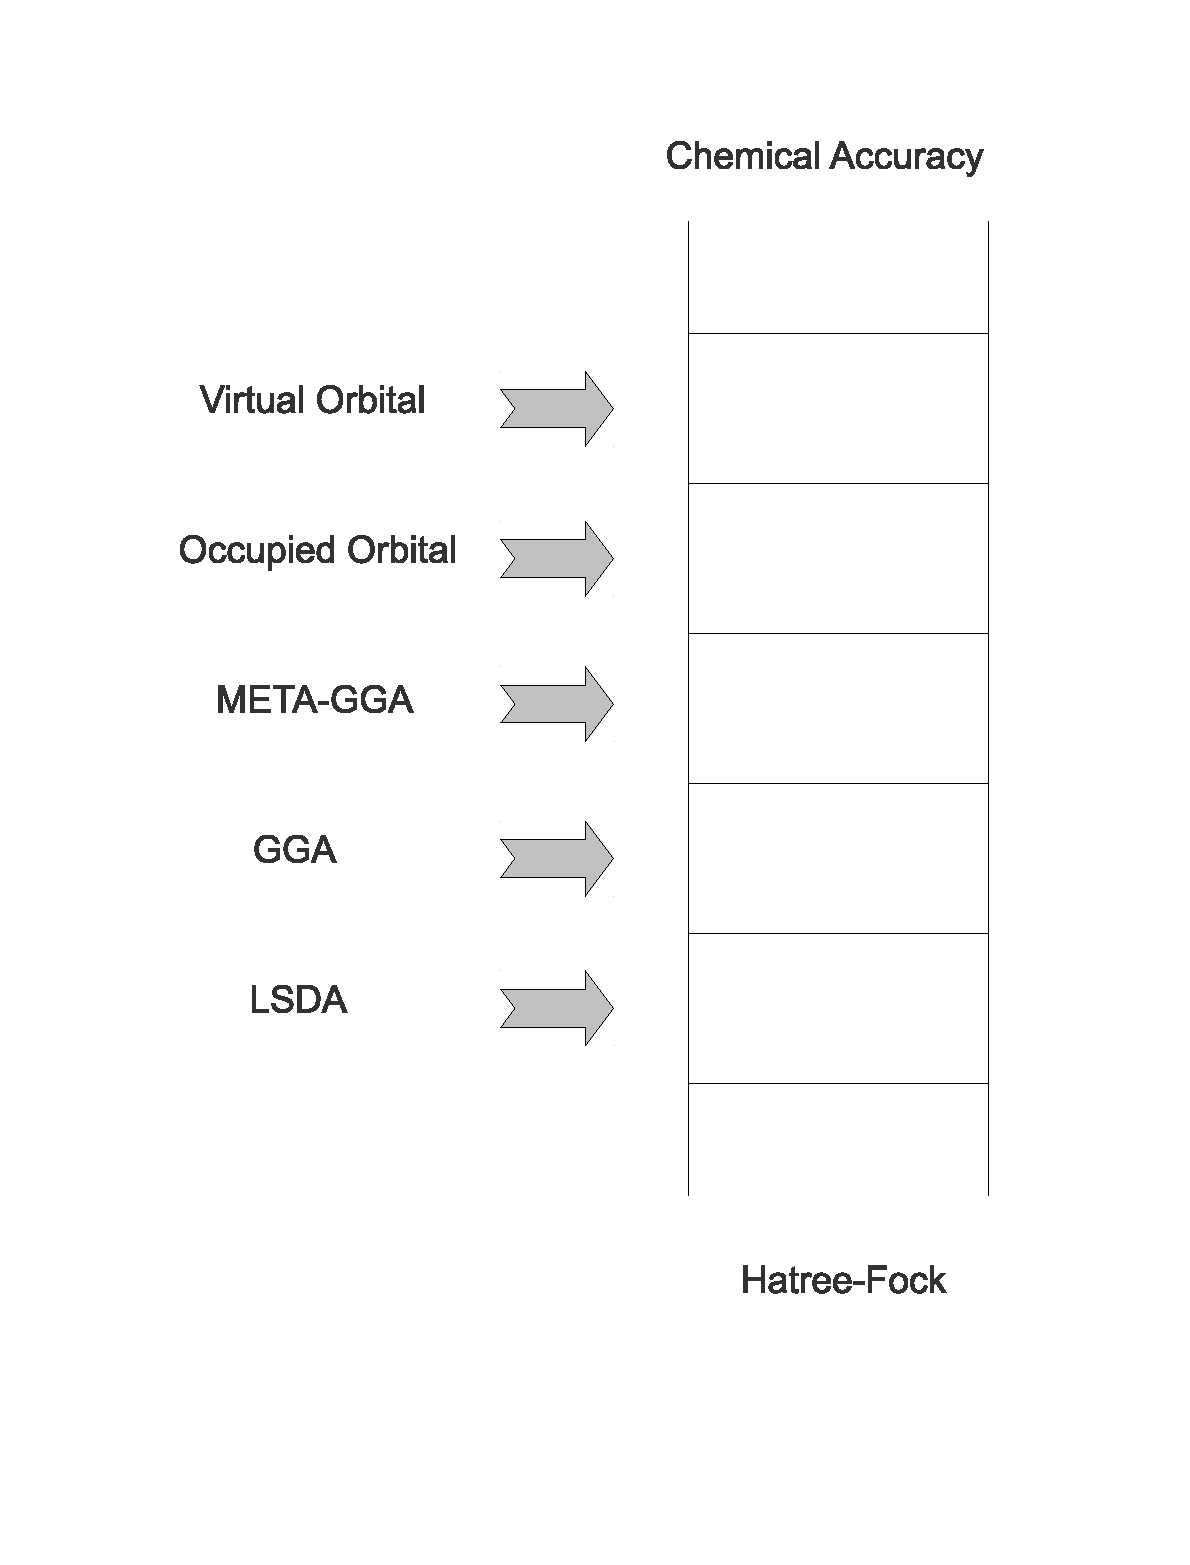
\includegraphics[scale=0.7]{jacob.eps}
\caption{Jacob's ladder for density functional approximation}
\end{center}
\end{figure}


%%%%%%%%%%%%%%%%%%%%%%%%%%%%%%%%%%%%%%%%%%%%%%%%%%%%%%%%%%%%%%%%%%%%%%%%%%%
\section{The Kohn-Sham equation}
\label{DFTI:4}
%
%
%
By this point, actually we have been set up all of the important
concepts for initialize the concrete calculation.

In the Kohn-Sham scheme, the approximated single electron wave
function for the non-interacting system is used to minimize the
total energy expression we have gotten in the (\ref{DFTIeq:24}).
Follows the tradition in the above section, here the $\theta_{i}$ is
employed to represent the Kohn-Sham orbital. And the $\phi$ is
always used to denote the atomic orbitals; so as to distinguish the
KS orbital. Furthermore, the condition for the Kohn-Sham orbitals is
just put forward in the (\ref{DFTIeq:27}) and (\ref{DFTIeq:28}).

Now the physical meaning of $\theta_{i}$ is clear. Since the
$\theta_{i}$ is the eigen states for single electron operator, then
we can use it to form some Slater determinant to represent the whole
quantum state:
\begin{equation}
\label{DFTIeq:11}
  \Theta_{KS}=\frac{1}{\sqrt{n!}}   \left | \begin{array}{cccc}
      \theta_{1}(1) & \theta_{2}(1) & \cdots & \theta_{n}(1) \\
      \theta_{1}(2) & \theta_{2}(2) & \cdots & \theta_{n}(2) \\
      \cdots & \cdots & \cdots & \cdots                      \\
      \theta_{1}(n) & \theta_{2}(n) & \cdots & \theta_{n}(n)
    \end{array} \right |
\end{equation}
Here we restrict ourself to the close shell case, hence the spin
state for the orbitals is not considered here. The $\Theta_{KS}$ has
the form: $|\Theta_{KS}|^{2}=\rho$.

So far the energy is expressed as:
\begin{equation}\label{}
  E[\rho]=T_{S}[\rho]+J[\rho]+E_{v}[\rho]+E_{XC}[\rho]
\end{equation}

With each term explicitly expressed in the energy expression, it
finally yields:
\begin{multline}\label{}
  E[\rho]=
  -\frac{1}{2}\sum_{i}^{n}\langle\theta_{i}(r)|\nabla^{2}|\theta_{i}(r)\rangle
  -\sum_{i}^{n}\sum_{A}^{N}\int\frac{Z_{A}}{r_{iA}}|\theta_{i}(r)|^{2}dr+ \\
  \frac{1}{2}\sum_{i}^{n}\sum_{j}^{n}
  \int\int|\theta_{i}(r)|^{2}\frac{1}{|r-r^{'}|}|\theta_{j}(r^{'})|^{2}drdr^{'}
  +E_{XC}[\rho(r)]
\end{multline}

Here we can strike up the variational search among the $\theta_{i}$,
just the same procedure which has been carefully described in the
chapter \ref{HFT}.

So the final KS equation is:
\begin{equation}\label{DFTIeq:12}
  \left [ -\frac{1}{2}\nabla^{2} + \hat{V}_{S}(r) \right ] \theta_{i}(r) =
  \epsilon _{i}\theta_{i}(r)
\end{equation}

The $\hat{V}_{S}(r)$ is:
\begin{equation}\label{DFTIeq:13}
  \hat{V}_{S} = v(r) + \sum_{i}^{n}\int\frac{|\theta_{i}(r^{'})|^{2}}
  {|r-r^{'}|}\,\,
  dr^{'}
  + \frac{\delta E_{XC}[\rho]}{\delta \rho(r)}
\end{equation}

Here let me note something more for the functional for the classic
electron repulsion:
\begin{align}\label{}
J[\rho] &=
\frac{1}{2}\int\int\frac{\rho(r)\rho(r^{'})}{|r-r^{'}|}drdr^{'}
\Rightarrow \nonumber \\
J[\rho] + J[\delta\rho] &= \frac{1}{2}\int\int\frac{(\rho(r) +
\delta\rho(r))(\rho(r^{'}) +
\delta\rho(r^{'}))}{|r-r^{'}|}drdr^{'} \Rightarrow \nonumber \\
J[\delta\rho] &= \frac{1}{2}\int\int\frac{\rho(r)
\delta\rho(r^{'})}{|r-r^{'}|}drdr^{'} +
\frac{1}{2}\int\int\frac{\delta\rho(r)\rho(r^{'})}{|r-r^{'}|}drdr^{'}
\nonumber \\
&=\int\int\frac{\rho(r)\delta\rho(r^{'})}{|r-r^{'}|}drdr^{'}
\end{align}
Theretofore, the factor of $1/2$ has been removed in the functional.
More discussion about the derivatives for the energy and functional
will be shown in the following content.


%%%%%%%%%%%%%%%%%%%%%%%%%%%%%%%%%%%%%%%%%%%%%%%%%%%%%%%%%%%%%%%%%%%%%%%%%%%%%
\section{Spin polarized Kohn-Sham function}
%
%
%
%
Now let's introduce spin polarized Kohn-Sham function, which is some
simple extension to the Kohn-Sham equation we have introduced.

In the density matrices section, we have known that the density
matrices actually depending on the spin variables on the location of
$r$ (see the section \ref{DODM_in_density_matrices}). Therefore, we
can also consider the up and down spin as separate variables, so to
define the spin density as:
\begin{equation}
\label{eq:FIDFTeq:76} \rho_{\sigma}(r) = n \int |\Psi(r, \sigma,
x_{2}, x_{3}, \cdots, x_{n})|^{2} dx_{2}dx_{3}\cdots dx_{n}
\end{equation}
While here the $\rho_{\sigma}(r)d^{3}r$ characterizes the density to
find an electron of spin $\sigma$ in $d^{3}r$ around the location of
$r$. Usually the spin density is characterized as $\rho^{\alpha}(r)$
and $\rho^{\beta}(r)$, or the $Q(r) = \rho^{\alpha}(r) -
\rho^{\beta}(r)$ plus the total density $\rho(r) = \rho^{\alpha}(r)
+ \rho^{\beta}(r)$.

So why we introduce the spin density into the Kohn-Sham equation?
Firstly, it's some necessary generalization for the system in
presence of an external magnetic field. For example, the electron
spin susceptibility, and the spin-orbit-coupling etc. They can be
only included within the spin density framework.

However, the major advantage for the spin polarized Kohn-Sham
function is that it leads to some more accurate system description.
For example, for the system with unpaired electrons, such as $Li$
atoms; the spin up density is unable to equal to the spin down type
density; so the close shell type of description is surely bad for
this situation.

Now let's go to see how to express the Kohn-Sham equation in the
spin density framework. Since the spin variable is introduced, the
Kohn-Sham orbital in the non-interacting system should also include
the spin variables; so that the Kohn-Sham orbitals should satisfy
the condition below (here we use $p$ to signal the $\alpha$
electron, and $q$ to designate the $\beta$ electrons):
\begin{align}
  \label{DFTIeq:77}
    \sum_{i=1}^{p}\theta^{2}_{i\alpha}(r) &=
    \rho^{\alpha}(r) \nonumber \\
    \sum_{i=1}^{q}\theta^{2}_{i\beta}(r) &=
    \rho^{\beta}(r)
\end{align}
While the non-interacting restriction requires that the
orthogonality condition that:
\begin{equation}
  \label{DFTIeq:78}
\int \theta^{*}_{i\sigma}(r)\theta_{j\sigma^{'}}(r) d\bm{r} =
\delta_{ij}\delta_{\sigma\sigma^{'}}
\end{equation}

Based on the (\ref{DFTIeq:77}) and (\ref{DFTIeq:78}), compared with
the (\ref{DFTIeq:11}) we can construct the spin dependent Slater
determinant as:
\begin{equation}
\label{DFTIeq:79} \Theta_{KS} =
 \begin{vmatrix}
         \theta_{1}(1)\alpha(1)  & \cdots  & \theta_{p}(1)\alpha(1)
       & \theta_{p+1}(1)\beta(1) & \cdots  & \theta_{n}(1)\beta(1)  \\
         \theta_{1}(2)\alpha(2)  & \cdots  & \theta_{p}(2)\alpha(2)
       & \theta_{p+1}(2)\beta(2) & \cdots  & \theta_{n}(2)\beta(2)  \\
          \cdots                 & \cdots  & \cdots
       &  \cdots                 & \cdots  & \cdots                  \\
         \theta_{1}(n)\alpha(n)  & \cdots  & \theta_{p}(n)\alpha(n)
       & \theta_{p+1}(n)\beta(n) & \cdots  & \theta_{n}(n)\beta(n)  \\
       \end{vmatrix}
\end{equation}
We can see that the (\ref{DFTIeq:79}) is similar to the UHF wave
function we get in the (\ref{HFTeq:45}). By the similar procedure,
we can also get the total energy expression:
\begin{multline}
  \label{DFTIeq:80}
  E[\rho^{\alpha}, \rho^{\beta}] =
\sum^{p+q}_{i\sigma} \left\langle\theta_{i\sigma}
\left|-\frac{1}{2}\nabla^{2}\right| \theta_{i\sigma}\right\rangle +
\frac{1}{2}\sum^{p+q}_{i\sigma}\sum^{p+q}_{j\sigma^{'}} \langle
\theta_{i\sigma}\theta_{j\sigma^{'}}|\frac{1}{r -
  r^{'}}|
\theta_{i\sigma}\theta_{j\sigma^{'}} \rangle \\
+ \int v(r)\rho^{\alpha}(r)d^{3}r + \int v(r)\rho^{\beta}(r)d^{3}r +
E_{XC}[\rho^{\alpha}, \rho^{\beta}]
\end{multline}

Here we can see that the kinetic part and the classic coulomb part
are independent to the spin variables.

Then, the variational research is carried out under the
orthogonality restriction in the (\ref{DFTIeq:78}), similar to the
treatment in the part of (\ref{RHFUHF_in_HF}), we can get a pair of
functions:
\begin{align}
\label{DFTIeq:81} \left[-\frac{1}{2}\nabla^{2} +
  V_{\alpha}(r)\right]\theta_{i\alpha}(r) &=
\epsilon_{i\alpha}\theta_{i\alpha}(r) \nonumber \\
\left[-\frac{1}{2}\nabla^{2} +
  V_{\beta}(r)\right]\theta_{i\beta}(r) &=
\epsilon_{i\beta}\theta_{i\beta}(r)
\end{align}

Where the spin dependent effective potentials are:
\begin{align}
  \label{DFTIeq:82}
V_{\alpha}(r) &= v(r) + \int\frac{\rho(r^{'})}{r -
  r^{'}}dr^{'} +
\frac{\delta E_{XC}[\rho^{\alpha}, \rho^{\beta}]}{\delta
  \rho^{\alpha}(r)} \nonumber \\
V_{\beta}(r) &= v(r) + \int\frac{\rho(r^{'})}{r -
  r^{'}}dr^{'} +
\frac{\delta E_{XC}[\rho^{\alpha}, \rho^{\beta}]}{\delta
  \rho^{\beta}(r)}
\end{align}

Now we can see that the results is very similar to the UHF
framework, however; they retains very different physical meanings.



%%%%%%%%%%%%%%%%%%%%%%%%%%%%%%%%%%%%%%%%%%%%%%%%%%%%%%%%%%%%%%%%%%%%%%%%%%%%%
\section{Further discussion for the $T_{S}[\rho]$}
\label{DFTI:3}
%
%  what's the relation between the Ts[\rho] and T[\rho]?
%  another understanding about the $T_{S}[\rho]$
%
Through the Kohn-Sham equation in (\ref{DFTIeq:12}), we can get the
KS orbital of $\theta_{i}(r)$ to minimize the whole energy so that to
get the expression of $T_{S}[\rho]$. However, as in the derivation of total
energy expression, we have a question that how to understand the physical
meaning of $T_{s}[\rho]$? Here we will have an answer.

Firstly we can define the $T_{S}[\rho]$ in some constrained search way:
\begin{equation}\label{}
\begin{split}
T_{S}[\rho] &= \min_{\Psi_{D} \rightarrow \rho}
\langle\Psi_{D}|\hat{T}|\Psi_{D}\rangle \\
    &= \min_{\sum_{i=1}^{n}|\psi_{i}|^{2} \rightarrow \rho}
    \left[\sum_{i=1}^{n}\int\psi^{*}_{i}(r)
    \left(-\frac{1}{2}\nabla^{2}\right)\psi_{i}(r)dr\right]
\end{split}
\end{equation}
Here the $\Psi_{D}$ indicates the anti-symmetric $n$ non-interacting 
electron wave functions, and it's composed by some $n$ non-interacting
orbitals of $\psi_{i}$. The constraint search is over all the $\Psi_{D}$ 
which gives the real density of $\rho$.

Interestingly we can prove that such definition can also lead to the
Kohn-Sham equation in (\ref{DFTIeq:12}). Firstly let's define some
functional:
\begin{multline}\label{}
\Omega(\psi_{1}, \psi_{2}, \cdots, \psi_{n}) =
\sum_{i=1}^{n}\int\psi^{*}_{i}(r)
    \left(-\frac{1}{2}\nabla^{2}\right)\psi_{i}(r)dr \\
    +
\int\lambda(r)\left\{\sum_{i=1}^{n}|\psi_{i}(r)|^{2}
-\rho(r)\right\}dr -
\sum_{ij}^{n}\epsilon_{ij}\int\psi^{*}_{i}(r)\psi_{j}(r)dr
\end{multline}
Here inside the $\Omega$ we have introduced the Lagrangian
multiplier of $\lambda(r)$ and $\epsilon_{ij}$. $\lambda(r)$ is used
to make sure that the density between the non-interacting system and
the real system is same, and $\epsilon_{ij}$ is used to require the
orthogonality between the non-interacting of $\psi_{i}(r)$.

The energy minimization condition is given by:
\begin{equation}\label{}
\frac{\partial \Omega}{\partial \psi_{k}} = 0 \quad k=1, 2, \cdots,
n
\end{equation}
Then we can get the resulting equation:
\begin{equation}\label{DFTIeq:16}
\begin{split}
  \hat{h}_{s}\psi_{k}(r) &= \sum_{l=1}^{n}\epsilon_{kl}\psi_{l}(r) \\
    \hat{h}_{s} &=-\frac{1}{2}\nabla^{2} + \lambda(r)
\end{split}
\end{equation}
Hence, the $\lambda(r)$ can be viewed as some local potential which
is just corresponding to the $\hat{V}_{s}(r)$ in (\ref{DFTIeq:13}),
and the $\psi_{k}(r)$ is just corresponding to the $\theta_{i}(r)$
in (\ref{DFTIeq:12}). On the other hand, such derivation is giving
the same Kohn-Sham equation again! Hence we can say, the physical 
meaning of non-interacting orbitals in Kohn-Sham framework is to 
minimize the $T_{s}[\rho]$.

Now let's proceed to another question that how close between the
$T_{S}[\rho]$ and the real kinetic energy in DFT?

Before answering the question, we should make it clear that how to
express the real kinetic energy in DFT. According to Levy constraint
search in (\ref{DFTI:1}), the kinetic energy as well as the
repulsion energy in DFT can given by the functional of
$F_{HK}[\rho]$:
\begin{equation}\label{}
F_{HK}[\rho] = \min_{\psi\rightarrow\rho}
\langle\psi|T+V_{ee}|\psi\rangle
\end{equation}
Where the $\psi$ indicates all the wave functions which give the
density of $\rho$. If we label the kinetic energy in the
$F_{HK}[\rho]$ as $T[\rho]$, then simply we can have:
\begin{equation}\label{DFTIeq:14}
T_{S}[\rho] \leq T[\rho]
\end{equation}
Since the wave function of $\psi$ in the $F_{HK}[\rho]$ may not
corresponding to the wave function which is just minimizing the
kinetic energy. Here the proof is just paraphrastic, the more strict
proof should refer to the material given by Weitao\cite{weitaoYang}.

The inequation in (\ref{DFTIeq:14}) has some significant consequence
that the exchange correlation functional contains some positive
component of kinetic energy. In the discussion related to the
functional, we will analyze it again.

%%%%%%%%%%%%%%%%%%%%%%%%%%%%%%%%%%%%%%%%%%%%%%%%%%%%%%%%%%%%%%%%%%%%%%
\section{How to code the exchange-correlation energy}
\label{sec:XC_functional}
%
%
%
%
Now in this section, we are going to give a discussion that how to
code the conceptual XC functional so that we can calculate the energy,
first and second derivatives etc. within DFT framework. For
simplicity, let's restricted the discussion within the ground state
DFT calculation first.

In the ground state DFT calculation, compared with the traditional
wave function method; there are two things we needed to get the
information of the system we study:
\begin{align}
 \label{eq:XC_functional.1}
\text{wave function} &\Leftrightarrow \text{electron density}
\nonumber
\\
\text{operator on the wave function} &\Leftrightarrow \text{functional
  on the density}
\end{align}
The density here we are talking about, is the electron density from
the non-interacting system which is in one to one mapping relationship
with the real system. Through the imaginary Kohn-Sham orbitals (see
\ref{DFTI:2} for more information), we can construct the electron
density for the real system.

On the other hand, how can we derive the electron density? We have
Kohn-sham equation, which is similar with Hatree-Fock equation (more
details about the KS equation please see \ref{DFTI:4}), through that
equation the trial density firstly generated by guess will be renewed,
then the newer electron density will be brought into the whole
function again until the self-consistent condition is met. Finally, by
the result electron density we can evaluate all the system information
we need.

In the Kohn-Sham equation in (\ref{DFTIeq:12}), we have an item which
contains the exchange and correlation energy, its general form has
been detailed discussed in the chapter \ref{Functionals_in_DFT}. In
that chapter, we derived the general relation between energy and the
density, the gradient of density or even the Laplacian of density
(in meta-GGA form) from the fundamental physical laws, and finally
their explicit forms are finally gotten. If both of the explicit form
of XC functional and the trial density is known, we can get the result
density through KS equation.

Finally, there's a question left that how to construct the trial
density, or more properly to say, the trial Kohn-Sham orbitals? In
principle, we can find enormous ways to do this, but in practice we
construct the trial density from the traditional AO basis set
functions, in other words;  the GTO or STO functions:
\begin{align}
  \label{eq:XC_functional.2}
\phi_{i} &= \sum_{j}d_{ij}\chi_{j} \Rightarrow \nonumber \\
\varphi_{i} &= \sum_{j}^{n}c_{ij}\phi_{i} \Rightarrow \nonumber \\
\rho_{trial} &= \sum_{i}^{occ}\varphi_{i}^{*}\varphi_{j} \nonumber \\
&=
\sum_{i}^{occ}\sum_{j}^{n}\sum_{k}^{n}c_{ij}^{*}c_{ik}\phi_{j}^{*}
\phi_{k}
\nonumber \\
&= \sum_{j}^{n}\sum_{k}^{n}P_{jk}\phi_{j}^{*}\phi_{k}
\end{align}
Here, the $\chi$ is the basic functions to form the basis set
functions
$\phi$, the $\chi$ can be GTO or STO; but mostly we use GTO. Here in
this step, the basis set functions are same between the wave function
method and the new DFT method. Then based on the basis set functions
of $\phi$, we can construct the trial Kohn-Sham orbitals of $\varphi$,
so finally we can get the trial density. Here above the $P_{jk}$ is
the density matrix for the basis function of $\phi_{j}$ and
$\phi_{k}$. 

Here we have something important to mention. In real culculation, we
always use basis sets in quantum chemistry, that is to say; all the
function space are built from some ``delicately selected'' basis
functions:
\begin{align}
 \label{basis_idea_funtional_eq:1}
\text{GTO (STO)} &\longrightarrow \text{AO  (basis sets)} \nonumber \\
\text{AO} &\longrightarrow \text{MO} \nonumber \\
\text{MO} &\longrightarrow \text{Slater determinants}
\end{align}
Here in such process, the basic function (GTO or STO) are fixed, the
forming of function space are all depending on their coefficients.
Specifically, in the (\ref{eq:XC_functional.2}) each basis sets of
$\phi_{i}$ is fixed, the coefficient of $d_{ij}$ and $\chi_{j}$ (GTO
or STO) are all pre-determined. On the other hand, $c_{ij}$ are
varied according to the energy variation process (could be HF method
or Kohn-Sham method), so the $\varphi_{i}$ (MO) are just some
variation results based on the space expanding by the $c_{ij}$. So
here we can see that $c_{ij}$ is the only thing varied, and we are
seeking for in energy calculation. 

In practice, the coefficient of the $c_{ij}$ is in $n\times n$
dimension ($n$ basis sets forming $n$ MOs). On the other hand, we can
also use the density matrix of $P_{ij}$ to equivalently express the
space of $c_{ij}$ (it's also in $n\times n$ dimension). Hence the
enegy variation process can be viewed as:
\begin{equation}
 \label{basis_idea_funtional_eq:2}
E = \Psi (q, P_{ij}, \cdots)
\end{equation}  
This is the central idea we applied across the quantum software.

Finally, let's come back to the solving of KS equation. if we
compare the HF equation and the KS equation, we can
find out that the only difference btween them is that there's a new
item of $E_{XC}$ in KS equation (here the point is aiming at the
hybrid functionals because it contains the HF exchange part, for
pure functional method such as BLYP; there's no HF exchange part),
and all the other terms are kept to be same. Hence let's proceed to
discuss the formation of $E_{XC}$ in details.

%%%%%%%%%%%%%%%%%%%%%%%%%%%%%%%%%%%%%%%%%%%%%%%%%%%%%%%%%%%%%%%%%%%%%%


%%% Local Variables:
%%% mode: latex
%%% TeX-master: "../../main"
%%% End:

%%
% change log:
% originally setting up around the Jan. 2009,
% begin to revise at end of the June.
% 1 revise the Thomas-Fermi model, derive the kinetic energy 23th, June
% 2 derive the exchange energy 24th, June
% 3  change the hbar in the former content into h, correct a bug
% revise from July 8th to 15th, 2009:
% rewrite the whole uniform electron gas analysis, and the discussion with
% kinetic energy and exchange energy
%

\chapter{Functionals in Density Functional Theory}
\label{Functionals_in_DFT}
%%%%%%%%%%%%%%%%%%%%%%%%%%%%%%%%%%%%%%%%%%%%%%%%%%%%%%%%%%%%%%%%%%%%%%%%%%%%

After establishing the main framework of the Kohn-Sham equations,
there's some important work left for us, which is to find the concrete
expression of the $E_{XC}$. This part of work is the essence of DFT
theory, and it's the most important and difficult task that the theory
meets. So in this chapter, we are trying to review this part of work
in general, and most importantly to get the core idea of this part of
work.



%%%%%%%%%%%%%%%%%%%%%%%%%%%%%%%%%%%%%%%%%%%%%%%%%%%%%%%%%%%%%%%%%%%%%%%%%%%%%
\section{General idea for the $E_{XC}$ in DFT}
%
%
%
%
According to the discussion made in the last chapter(\ref{DFTIeq:29}), the
$E_{XC}$ is generally expressed as:
\begin{align}
  \label{FIDFTeq:90}
  E_{XC}[\rho] &= T[\rho] - T_{S}[\rho] + E_{X}[\rho] + E_{C}[\rho]
\nonumber \\
&=
\frac{1}{2}\int^{\lambda = 1}_{\lambda = 0} \int
\left(\frac{1}{r_{12}}\right)
\rho(r_{1})\rho(r_{2})(g_{\lambda}(r_{1},
r_{2})-1)d^{3}r_{1}d^{3}r_{2} d\lambda \nonumber \\
&=\frac{1}{2} \int \left(\frac{1}{r_{12}}\right)
\rho(r_{1})\rho(r_{2})\widetilde{h}(r_{1},
r_{2})d^{3}r_{1}d^{3}r_{2}
\end{align}


This is some important starting point for getting the concrete form
of $E_{XC}$, and it will be used later in the following part of this
chapter.

However, only the general expression in (\ref{FIDFTeq:90}) is not
enough to derive the concrete form of $E_{XC}$. Hence how can we
derive the concrete form of $E_{XC}$?

The first step is the so called ``LDA'' approximation. Generally, 
this model assumes that all the electron densities are homogeneous 
among all the space, so we have $\rho(r)$ as some constant. Finally, 
in the (\ref{FIDFTeq:90}) we can 
integrate over $r_{2}$, that leads to:
\begin{equation}
 \begin{split}
  E_{XC}[\rho] &= \frac{1}{2} \int \left(\frac{1}{r_{12}}\right)
\rho(r_{1})\rho(r_{2})\widetilde{h}(r_{1},
r_{2})d^{3}r_{1}d^{3}r_{2} \\
&= \int d^{3}r_{1} \rho(r_{1}) 
\left\lbrace 
\frac{1}{2}\int  
\left(\frac{1}{r_{12}}\right)\rho(r_{2})\widetilde{h}(r_{1},
r_{2})d^{3}r_{2}
\right\rbrace  \\
&= \int d^{3}r_{1} \rho(r_{1}) v(r_{1})
 \end{split}
 \label{FIDFTeq:91}
\end{equation}
Here we can see that the $\widetilde{h}(r_{1},
r_{2})$ is integrated over $r_{2}$ which implies that the 
exchange-correlation effects are considered in the average way (just like
the HF wave function). This expression is the general exchange-correlation
energy expression for LDA model.

Gnerally speaking, to approach a concrete XC expression means
we need to find some ``simple'' but ``representative'' physical 
model. From this model, perhaps we can get the exact
wave functions and the corresponding energy levels. Then by using
some physical tools such as the statistical method and the
mathematical tricks, we can get the relation between the electron
density and the corresponding energies (for example, the kinetic
energy, exchange energy etc.). By then, the $E_{XC}$ can be gotten.
In the following sections, we will how to do this within LDA 
approximation.

From the discussion in the (\ref{DFTI:1}), we have known that the
$E_{XC}$ is invariant to any nucleus configurations as well as any
electron densities. Hence it can be well expected that if the
general expression of $E_{XC}$ is gotten, then it can be applied to
any chemistry system from the $H_{2}$ molecule to the complex
protein molecules. Therefore, the $E_{XC}$ is universal in this
point.


%%%%%%%%%%%%%%%%%%%%%%%%%%%%%%%%%%%%%%%%%%%%%%%%%%%%%%%%%%%%%%%%%%%%%%%%%%%%%
\section{Local density approximation}
%
%
%
%
Actually there has some physical model which is paradigm for
deriving the exchange-correlation energy, this is the ``uniform
electron gas model''\cite{DFT_PAPERS_GATHERING,
Peter_Fulde_electron_gas}; which is corresponding to the famous
local density approximation (LDA) in density functional theory.

In this model, the electrons are trapped into some periodically
arranged cubic box with volume of $V=l^{3}$, therefore the electron
states repeat from one face of cube to its opposite face. Inside the
box, there has evenly spreaded positive charge background so that
the total system is able to keep to be neutral, so the electrons are
inhabited in some homogeneous medium.  Furthermore, we assume that
there's no potential of $\hat{V}$ inside the box, so the motion of
electrons can be described by free particle wave function.

Since the free electron model requires that the electron density is
constant, then as $l\uparrow$, the number of electrons inside the cube
must also increase so that to make $\frac{N}{V}$ is some
constant. Therefore, in the content below we do not explicitly assign
the average electron density as some function of $r$ if necessary.

Now let's step into mathematical details. Suppose that the box is
located in the direction below:
\begin{equation}
  \label{eq:FIDFTeq:16}
\hat{V} = 0 \quad (0< x, y, z < l)
\end{equation}
And the boundary condition is:
\begin{equation}
  \label{eq:FIDFTeq:17}
 \left\{
  \begin{array}{ll}
    \hat{V}(x+nl,y,z) = \hat{V}(x,y,z), & \hbox{$n = 0, \pm 1, \pm 2 \cdots$} \\
    \hat{V}(x,y+nl,z) = \hat{V}(x,y,z), & \hbox{$n = 0, \pm 1, \pm 2 \cdots$} \\
    \hat{V}(x,y,z+nl) = \hat{V}(x,y,z), & \hbox{$n = 0, \pm 1, \pm 2 \cdots$}
  \end{array}
\right.
\end{equation}
While $n<0$ indicates that the boxes are extending to the negative
direction of the coordinate system.

Now let's consider the wave function for the (\ref{eq:FIDFTeq:16})
and (\ref{eq:FIDFTeq:17}), it should be:
\begin{align}\label{eq:FIDFTeq:18}
\Psi(k_{x}, k_{y}, k_{z}) &= \frac{1}{l^{\frac{2}{3}}}e^{i(k_{x}x+
k_{y}y+k_{z}z)} \nonumber \\
&=\frac{1}{V^{\frac{1}{2}}}e^{i \mathbf{k}\cdot \mathbf{r}}
\end{align}
Here $\mathbf{k}$ is the corresponding wave vector, and it's
related to the principal quantum number:
\begin{equation}\label{eq:FIDFTeq:19}
k_{x}=\frac{2\pi}{l}n_{x} \quad k_{y}=\frac{2\pi}{l}n_{y} \quad
k_{z}=\frac{2\pi}{l}n_{z}
\end{equation}
Where the $n_{x}, n_{y}, n_{z}$ can adopt $0, \pm 1, \pm 2, \cdots$.

The corresponding energy is:
\begin{align}\label{eq:FIDFTeq:20}
E(n_{x}, n_{y}, n_{z}) &= \frac{h^{2}}{8ml^{2}}[(2n)^{2}_{x} +
(2n)^{2}_{y} + (2n)^{2}_{z}] \nonumber \\
&=\frac{h^{2}}{4\pi^{2}}\left[\frac{k_{x}^{2}}{2m} +
\frac{k_{y}^{2}}{2m} + \frac{k_{z}^{2}}{2m}\right]
\end{align}

If we have:
\begin{equation}
  \label{eq:FIDFTeq:49}
  k^{2} = k_{x}^{2} + k_{y}^{2} + k_{z}^{2}
\end{equation}
Then the corresponding energy is converted to:
\begin{equation}
  \label{eq:FIDFTeq:50}
  E_{k} = \frac{\hbar^{2}}{2m}k^{2}
\end{equation}

Now we assume that within the cube of $V$ there are many electrons
resided in, and we can use the statistical method to evaluate the
density.

Firstly, since that there's only finite number of electrons, then
there must have some energy level on which no electrons residing
in. the highest energy level while the electron occupied is called
``Fermi energy'', and it's labeled as $\epsilon_{F}$. Then according
to Fermi-Dirac statistics, the average number of electrons on
certain energy level of $E_{k}$ is:
\begin{equation}
  \label{eq:FIDFTeq:51}
  n_{k} = \frac{1}{e^{\frac{E_{k}-\epsilon_{F}}{k_{B}T}} + 1}
\end{equation}
$k_{B}$ is the Boltzmann's constant. Then we can evaluate the total
electron number as:
\begin{equation}
  \label{eq:FIDFTeq:52}
  N= 2\sum_{k=-\infty}^{k=+\infty}n_{k} =
  2\sum_{k=-\infty}^{k=+\infty}\frac{1}{e^{\frac{E_{k}-\epsilon_{F}}{k_{B}T}}
    + 1}
\end{equation}
Here the multiplier of $2$ is because that each single electron state
is occupied by two electrons with opposite spin.

By the way, through the (\ref{eq:FIDFTeq:51}) the Fermi energy can be
gotten some clear physical interpretation. At absolute zero
temperature, the occupation number is $1$ for energies less than the Fermi
energy and zero for energies greater than the Fermi energy. Such
situation is pictured in the (\ref{FIDFT:1}).

\begin{figure}
\begin{center}
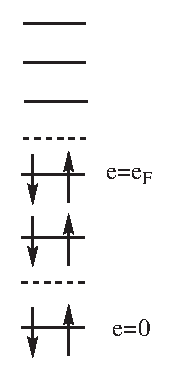
\includegraphics[scale=0.7]{DFT_Fermi.eps}
\caption{Electrons arrangement for uniform electron gas model at $0$k}
\label{FIDFT:1}
\end{center}
\end{figure}

If there are many electron states, then the summation process in
(\ref{eq:FIDFTeq:52}) can be transformed into the integral:
\begin{align}
  \label{eq:FIDFTeq:53}
 N &= 2\int \int \int \frac{1}{e^{\frac{E_{k}-\epsilon_{F}}{k_{B}T}}
    + 1}dn_{x}dn_{y}dn_{z} \nonumber \\
   &= 2\int \int \int \frac{1}{e^{\frac{E_{k}-\epsilon_{F}}{k_{B}T}}
    +
    1}\frac{dk_{x}}{2\pi/l}\frac{dk_{y}}{2\pi/l}\frac{dk_{z}}{2\pi/l}
  \nonumber \\
   &= 2\frac{V}{(2\pi)^{3}}\int \int \int \frac{1}{e^{\frac{E_{k}-\epsilon_{F}}{k_{B}T}}
     + 1}dk_{x}dk_{y}dk_{z}
\end{align}

However, the integration in the (\ref{eq:FIDFTeq:53}) is not
easy to get. Since we only have the energy as some function of
$k_{x}$, $k_{y}$ and $k_{z}$ (see \ref{eq:FIDFTeq:20}), then the
variation for the $k_{x}$, $k_{y}$ and $k_{z}$ are not independent; in
other words, we can not have the integration in the
(\ref{eq:FIDFTeq:53}) transformed into:
\begin{equation}\label{}
\int_{0}^{k_{max}}f(k_{x})dk_{x} \int_{0}^{k_{max}} g(k_{y})dk_{y}\int_{0}^{k_{max}}
h(k_{z})dk_{z}
\end{equation}

For solving this problem, we have to abandon the use the variables
of $(k_{x}, k_{y}, k_{z})$ so that to transform into the sphere
coordinate system of $(k, \theta, \phi$); where $k=\sqrt{k_{x}^{2} +
k_{y}^{2} + k_{z}^{2}}$.

Then we have (\ref{eq:FIDFTeq:53}) becomes:
\begin{equation}\label{eq:FIDFTeq:54}
N = 2\frac{V}{(2\pi)^{3}}
\int_{0}^{k_{F}}\int_{0}^{\pi}\int_{0}^{2\pi}
\frac{1}{e^{\frac{E_{k}-\epsilon_{F}}{k_{B}T}}
+ 1}k^{2}\sin\theta dkd\theta d\phi
\end{equation}

Here $k_{F}$ has very clear physical meaning, it equals to the maximum
value of $k$:
\begin{equation}
  \label{eq:FIDFTeq:55}
  k_{F} = \max \sqrt{k_{x}^{2} + k_{y}^{2} + k_{z}^{2}}
\end{equation}
Hence, $k_{F}$ characterizes the absolute maximum momentum of the wave
functions, it's easy to know that such wave function also gives the
Fermi energy of $\epsilon_{F}$.

Now let's go to see how to express the $k_{F}$. Suppose that it's in
absolute zero temperature, then the (\ref{eq:FIDFTeq:54}) simply
becomes:
\begin{align}
  \label{eq:FIDFTeq:56}
N &= 2\frac{V}{(2\pi)^{3}}
\int_{0}^{k_{F}}\int_{0}^{\pi}\int_{0}^{2\pi}k^{2}\sin\theta dkd\theta
d\phi
\nonumber \\
&= 2\frac{V}{(2\pi)^{3}}
\int_{0}^{k_{F}}k^{2}4\pi dk \nonumber \\
&=\frac{k_{F}^{3}}{3\pi^{2}}V
\end{align}

So far we can see that it's possible for us to associate the electron
density with the $k_{F}$:
\begin{equation}
  \label{eq:FIDFTeq:57}
\rho = \frac{N}{V} = \frac{k_{F}^{3}}{3\pi^{2}}
\end{equation}


%%%%%%%%%%%%%%%%%%%%%%%%%%%%%%%%%%%%%%%%%%%%%%%%%%%%%%%%%%%%%%%%%%%%%%%%%%%%%
\subsection{Kinetic energy derivation}
\label{KED_in_function}
%
%
%
%
Now let's evaluate the kinetic energy through the results above. From
the (\ref{eq:FIDFTeq:51}) and (\ref{eq:FIDFTeq:50}), we can express
the total energy as:
\begin{align}
  \label{eq:FIDFTeq:58}
e_{total} &= 2\sum_{k=-\infty}^{k=+\infty}E_{k}n_{k} \nonumber \\
        &= 2\sum_{k=-\infty}^{k=+\infty}
          \frac{\frac{\hbar^{2}}{2m}k^{2}}{e^{\frac{E_{k}-\epsilon_{F}}{k_{B}T}}
    + 1}
\end{align}

In the large number of wave vectors, the sum can be approximated as
integral (the treatment is similar to the \ref{eq:FIDFTeq:53}):
\begin{align}
  \label{eq:FIDFTeq:59}
e_{total} &= 2\frac{V}{(2\pi)^{3}}\int \int \int
\frac{\frac{\hbar^{2}}{2m}k^{2}}{e^{\frac{E_{k}-\epsilon_{F}}{k_{B}T}}
     + 1}dk_{x}dk_{y}dk_{z} \nonumber \\
&=  2\frac{V}{(2\pi)^{3}}
\int_{0}^{k_{F}}\int_{0}^{\pi}\int_{0}^{2\pi}
\frac{\frac{\hbar^{2}}{2m}k^{2}}{e^{\frac{E_{k}-\epsilon_{F}}{k_{B}T}}
+ 1}k^{2}\sin\theta dkd\theta d\phi
\end{align}

Now we consider the $T = 0$, then in the absolute zero temperature we
have the expression of (\ref{eq:FIDFTeq:59}) as:
\begin{align}
  \label{eq:FIDFTeq:60}
e_{total} &= 2\frac{V}{(2\pi)^{3}}
\int_{0}^{k_{F}}\int_{0}^{\pi}\int_{0}^{2\pi}
\frac{\hbar^{2}}{2m}k^{4}\sin\theta dkd\theta d\phi \nonumber \\
&=  2\frac{V}{(2\pi)^{3}}
\int_{0}^{k_{F}}\frac{\hbar^{2}}{2m}k^{4}4\pi dk \nonumber \\
&= \frac{\hbar^{2}}{m} \frac{V}{(2\pi)^{3}}4\pi\frac{k_{F}^{5}}{5}
\nonumber \\
&= \frac{\hbar^{2}}{m} \frac{V}{(10\pi)^{2}}k_{F}^{5}
\end{align}

The kinetic energy for each cube is actually the average of
$e_{total}$, this is $\frac{e_{total}}{V}$. Then by bringing the
(\ref{eq:FIDFTeq:57}) into (\ref{eq:FIDFTeq:60}), we can have:
\begin{align}
  \label{eq:FIDFTeq:61}
e_{kinetic} &= \frac{\hbar^{2}}{m}
\frac{3\pi^{2}}{(10\pi)^{2}}(3\pi^{2})^{\frac{2}{3}}\rho^{\frac{5}{3}}
\nonumber \\
&= \frac{\hbar^{2}}{m}
\frac{3}{10}(3\pi^{2})^{\frac{2}{3}}\rho^{\frac{5}{3}}
\end{align}

In the atom units, we have $\hbar = m = 1$, then the
(\ref{eq:FIDFTeq:61}) can be expressed as:
\begin{equation}
  \label{eq:FIDFTeq:62}
e_{kinetic} = \frac{3}{10}(3\pi^{2})^{\frac{2}{3}}\rho^{\frac{5}{3}}
\end{equation}
If we abbreviate the $\frac{3}{10}(3\pi^{2})^{\frac{2}{3}} = C_{F}$,
then the energy is:
\begin{equation}
  e_{kinetic} = C_{F}\rho^{\frac{5}{3}}
\end{equation}

Now let's consider the kinetic energy for all the space. In discrete
case, it has the expression that:
\begin{equation}
\label{eq:FIDFTeq:64}
E_{kinetic} = \sum_{V}e_{kinetic}V
\end{equation}
The summation is over all the cubic volumes. Now we make the volume of
$V$ getting smaller so that to make the cubic box tends to a point of
$\mathbf{r}$ in the space; in this case we can replace the summation
with the integration and have:
\begin{equation}
  \label{eq:FIDFTeq:63}
E = C_{F}\int\rho^{\frac{5}{3}}(r)dr
\end{equation}
Here as the cubic box becomes infinitely small; $V$ begin to approach
to $d\mathbf{r}$ so that the (\ref{eq:FIDFTeq:64}) can be safely
replaced by the (\ref{eq:FIDFTeq:63}). This is the final expression of
the kinetic energy in uniform electron gas model, and from the
(\ref{eq:FIDFTeq:63}) we can know that the functional for kinetic
energy is:
\begin{equation}
  \label{eq:FIDFTeq:65}
  \epsilon_{k}[\rho] = C_{F}\rho^{\frac{2}{3}}
\end{equation}


%%%%%%%%%%%%%%%%%%%%%%%%%%%%%%%%%%%%%%%%%%%%%%%%%%%%%%%%%%%%%%%%%%%%%%%%%%%%%
\subsection{Another way to derive The kinetic energy}
%
%
%
%
Now let's give some slightly different method to derive the
(\ref{eq:FIDFTeq:63}), this method is still based on the uniform
electron gas model; but it uses some different wave
functions\cite{weitaoYang}.

Compared with the periodic restrictions used in the
(\ref{eq:FIDFTeq:16}) and (\ref{eq:FIDFTeq:17}), here we assume that
the whole even extended space is divided into many pieces (each is
some small cubic box, we can call it cell with volume of $\Delta V =
l^{3}$); the electrons are considered to move in the cell and obey the
relations below:
\begin{equation}\label{eq:FIDFTeq:1}
\hat{V} = \left\{
    \begin{array}{ll} 0, & \hbox{ $0 < x,y,z < l$} \\ \infty, & \hbox{
$x,y,z<0, x,y,z>l$}
    \end{array} \right.
\end{equation}

Therefore such cell is equivalent to some three-dimensional infinite
well. The electronic wave function and the corresponding energy for
the cell is:
\begin{equation}\label{eq:FIDFTeq:2}
\psi_{n_{x}, n_{y}, n_{z}}(x,y,z) =
(\frac{8}{l^{3}})^{\frac{1}{2}} \sin (\frac{n_{x}\pi x}{l})\sin
(\frac{n_{y}\pi y}{l})\sin (\frac{n_{z}\pi z}{l}) \quad 0 < x,y,z < l
\end{equation}

\begin{equation}\label{eq:FIDFTeq:3}
\epsilon_{n_{x}, n_{y}, n_{z}} = \frac{h^{2}}{8ml^{2}}(n^{2}_{x} +
n^{2}_{y} + n^{2}_{z})
\end{equation}

Here, if we have:
\begin{equation}
  \label{eq:FIDFTeq:4}
  R^{2} = n^{2}_{x} + n^{2}_{y} + n^{2}_{z}
\end{equation}
Then the energy in (\ref{eq:FIDFTeq:3}) becomes:
\begin{equation}
  \label{eq:FIDFTeq:66}
\epsilon(R) = \frac{h^{2}}{8ml^{2}}R^{2}
\end{equation}

Similarly, for using the statistic tools we also assume that there are
many electrons resided in the cell, and we only consider the case as
$T=0$, which is the absolute zero temperature.

In large number of quantum states limits, similar to the $k$ we
consider that the $(n_{x}, n_{y}, n_{z})$ varies in continuous way.
Then we imagine the $(n_{x}, n_{y}, n_{z})$ corresponds to
each point in the three dimensional coordinate system, then all the
$(n_{x}, n_{y}, n_{z})$ points are located in the first quadrant so
that we can express the total number of electronic states of
$\Phi(\epsilon)$ as:
\begin{align}
  \label{eq:FIDFTeq:5}
  \Phi(\epsilon) &= \frac{1}{8}\left(\frac{4}{3}\pi R^{3}\right)
  \nonumber \\
  &=\frac{1}{8}\left[\frac{4}{3}\pi
    \left(\frac{8ml^{2}\epsilon}{h^{2}}\right)^{\frac{3}{2}}\right] \nonumber \\
  &=\frac{1}{6}\pi
    \left(\frac{8ml^{2}\epsilon}{h^{2}}\right)^{\frac{3}{2}}
\end{align}

Next we can evaluate the density of the total electronic states of
$\Phi(\epsilon)$:
\begin{align}
  \label{eq:FIDFTeq:6}
  g(\epsilon)\Delta\epsilon &= \Phi(\epsilon + \Delta\epsilon) -
  \Phi(\epsilon) \nonumber \\
  &=\frac{1}{4}\pi
    \left(\frac{8ml^{2}}{h^{2}}\right)^{\frac{3}{2}}\epsilon^{\frac{1}{2}}
    + O(\epsilon)
\end{align}
Physically the $g(\epsilon)$ characterizes the density of the
quantum states, has similar physical meaning with $n_{k}$ in the
(\ref{eq:FIDFTeq:51}).

Now through the $g(\epsilon)$, in principle we can calculate the total
energy of $\Delta E$ corresponding to the $\Phi(\epsilon)$:
\begin{equation}
  \label{eq:FIDFTeq:7}
  \Delta E = 2\int^{\infty}_{0}\epsilon g(\epsilon)d\epsilon
\end{equation}
In discrete case, this is equivalent to the expression that $E =
2\sum\epsilon_{i}n_{i}$. Here the multiplier of $2$ is because each
electronic state is double occupied.

Since that for any real system there's only infinite number of
electrons, thus for the $\epsilon$ it's only that $\epsilon <
\epsilon_{F}$ there's electrons residing in; so we can rewrite the
(\ref{eq:FIDFTeq:7}) as:
\begin{align}
  \label{eq:FIDFTeq:8}
    \Delta E &= 2\int^{\epsilon_{F}}_{0}\epsilon g(\epsilon)d\epsilon
    \nonumber \\
    &= 4\pi
    \left(\frac{2ml^{2}}{h^{2}}\right)^{\frac{3}{2}}\int^{\epsilon_{F}}_{0}
    \epsilon^{\frac{3}{2}}d\epsilon \nonumber \\
    &= \frac{8}{5}\pi
    \left(\frac{2ml^{2}}{h^{2}}\right)^{\frac{3}{2}}\epsilon^{\frac{5}{2}}
\end{align}

Similarly, the total number of electrons of $\Delta N$ within each
cell can be also calculated:
\begin{align}
  \label{eq:FIDFTeq:9}
      \Delta N &= 2\int^{\epsilon_{F}}_{0} g(\epsilon)d\epsilon
      \nonumber \\
      &= \frac{8}{3}\pi
    \left(\frac{2ml^{2}}{h^{2}}\right)^{\frac{3}{2}}\epsilon^{\frac{3}{2}}
\end{align}
Here in discrete case the $\Delta N$ is equivalent to $\Delta N =
\sum_{i}n_{i}$.

Now let's compare the (\ref{eq:FIDFTeq:8}) and (\ref{eq:FIDFTeq:9}),
it's clear that we can drop the $\epsilon_{F}$ and connect the $\Delta
N$ and $\Delta E$ together:
\begin{align}
  \label{eq:FIDFTeq:10}
  \Delta E &= \frac{3}{5}\Delta N \times \epsilon_{F} \nonumber \\
  &=\frac{3}{10}\frac{h^{2}}{m}\left(\frac{3}{8\pi}\right)^{\frac{2}{3}}
l^{3}\left\{\frac{\Delta N}{l^{3}}\right\}^{\frac{5}{3}}
\end{align}

Furthermore, if we switch to the atomic units and abbreviate the
constant part as:
\begin{align}
  \label{eq:FIDFTeq:11}
  C_{F} &= \frac{3}{10}\left(\frac{3}{8\pi}\right)^{\frac{2}{3}}
  \frac{h^{2}}{m} \nonumber \\
  &= \frac{3}{10}(3\pi^{2})^{\frac{2}{3}}
\end{align}
Here atomic units require that $\frac{h}{2\pi} = m_{e} = 1$. Here we
can see that the $C_{F}$ defined here is same to the $C_{F}$ defined
in the (\ref{eq:FIDFTeq:63}).

Then the (\ref{eq:FIDFTeq:10}) will finally be:
\begin{equation}
  \label{eq:FIDFTeq:12}
  \Delta E = C_{F}l^{3}\left\{\frac{\Delta N}{l^{3}}\right\}^{\frac{5}{3}}
\end{equation}

So far all the calculation are within in one cell. Here in the
(\ref{eq:FIDFTeq:12}) the expression of $\frac{\Delta N}{l^{3}}$ has
very clear physical meaning; it characterizes the average density
distribution in the cell. Now we counting all the cells, and have
$l\rightarrow 0$, then then the cell becomes infinitely small; $l^{3}$
begin to approach to some point of $d\mathbf{r}$ so that we can safely
replace the $l^{3}$ with $d\mathbf{r}$. In this case the expression of
(\ref{eq:FIDFTeq:12}) becomes:
\begin{equation}
  \label{eq:FIDFTeq:13} E = \sum \Delta E = C_{F}\int
\rho^{\frac{5}{3}}(r)dr
\end{equation}
Here as $l \rightarrow 0$ the summation over the discrete cells
naturally convert to the integration, and $l^{3} \rightarrow dr$. Then
we see that through some different method we still get the kinetic
energy expression in (\ref{eq:FIDFTeq:63}).



%%%%%%%%%%%%%%%%%%%%%%%%%%%%%%%%%%%%%%%%%%%%%%%%%%%%%%%%%%%%%%%%%%%%%%%%%%%%%%
\subsection{General form for local density approximation}
%
%
%
Here in the above derivation, there appears some important physical
idea about the model; which we call it as ``Local Density
Approximation'' or LDA shortly\cite{HK2}. In this approximation, electron
property are determined as functional of electron density by applying
local relations appropriate for some homogeneous electron system. Here
the key for the model is, the density should vary as slow as it can;
otherwise the model will fail.

as what we have showed, mathematically the LDA model can be expressed
as\cite{HK1}:
\begin{equation}
  \label{eq:FIDFTeq:67}
E^{LDA}_{XC} = \int \epsilon_{XC}[\rho(r)]\rho(r)d^{3}r
\end{equation}
Such expression has very clear physical meaning. Here the density of
$\rho(r)$ is the average electron number in the $V$ (actually the
density is keeping constant throughout the $V$), and
$\epsilon_{XC}[\rho(r)]$ is the average exchange and correlation
energy in this unit volume; hence their multiplication is the total
energy in the $V$. Then we can get the total energy by summing up
all the energy in $V$. As the volume is going to be infinitesimal,
the summation is transformed into the integration process, then we
can get the expression in the (\ref{eq:FIDFTeq:67}).

So far we have gotten the expression for the kinetic energy. Now
counting the electron repulsion and nuclear attraction part together
with kinetic energy, we can have:
\begin{equation}
\label{eq:FIDFTeq:14} E_{TF}[\rho] = \int
C_{F}\rho^{\frac{5}{3}}(r)d^{3}r - \int \rho(r)v(r)dr +
\frac{1}{2}\int\int
\frac{\rho(r_{1})\rho(r_{2})}{r_{12}}dr_{1}dr_{2}
\end{equation}

This formula can be used to estimate the total energy for the atom
system. However, in practice the (\ref{eq:FIDFTeq:14}) is demonstrated
to be over-simplified. It can not gave any molecule binding, and fail
to give correct shell structure for multi-electrons
atom\cite{weitaoYang}. But in despite of these problems, the Thomas-Fermi
model is still some clear physical model, and the concepts within it
lays the foundation for further discussion of functional.

%%%%%%%%%%%%%%%%%%%%%%%%%%%%%%%%%%%%%%%%%%%%%%%%%%%%%%%%%%%%%%%%%%%%%%%%%%%%%%
\subsection{Exchange energy derivation}
%
%
%
%
Now let's go to see how to derive the exchange functional through
the LDA model. This work was firstly done by
Dirac\cite{CambridgeJournals:2040328}, and
Slater\cite{PhysRev.81.385} used some different viewpoint to achieve
this functional again. Here the derivation of the exchange
functional is generally taken from Weitao's book\cite{weitaoYang}.

We start the topic from the density matrices in Hatree-Fock model. Now
consider some non-degenerate close shell ground state, it's total
energy expressed by density matrices can be gotten in the
(\ref{DMeq:34}); where in the close shell case we note that the
exchange energy can be expressed as:
\begin{equation}
\label{eq:FIDFTeq:15}
    E_{exchange} =  -\frac{1}{4}\int \frac{1}{r_{12}}
  |\rho_{1}(x_{1},x_{2})|^{2}dx_{1}dx_{2}
\end{equation}
Our derivation will start from the (\ref{eq:FIDFTeq:15}).


Now let's start from the wave function shown in the
(\ref{eq:FIDFTeq:18}). By using such wave functions, we can get the
expression for the $\rho_{1}(x_{1},x_{2})$:
\begin{align}
\label{eq:FIDFTeq:22}
\rho_{1}(\mathbf{r_{1}}, \mathbf{r_{2}}) &=
2\sum_{occupied}\Psi^{*}(\mathbf{r_{1}})\Psi(\mathbf{r_{2}}) \nonumber \\
&=\frac{2}{V}\sum_{occupied}e^{i\mathbf{k}\cdot
(\mathbf{r_{2}}-\mathbf{r_{1}})} \nonumber \\
&=\frac{2}{V} \int
e^{i\mathbf{k}\cdot
(\mathbf{r_{2}}-\mathbf{r_{1}})}dn_{x}dn_{y}dn_{z} \nonumber \\
&=\frac{2}{V}\frac{V}{8\pi^{3}}\int e^{i\mathbf{k}\cdot
(\mathbf{r_{2}}-\mathbf{r_{1}})}dk_{x}dk_{y}dk_{z} \nonumber \\
&=\frac{1}{4\pi^{3}}\int e^{i\mathbf{k}\cdot
(\mathbf{r_{2}}-\mathbf{r_{1}})}dk_{x}dk_{y}dk_{z}
\end{align}

Here we consider that $n$ is continuously changed. Similar to the
treatment in the (\ref{eq:FIDFTeq:54}), we have to switch from the
$(k_{x}, k_{y}, k_{z})$ to the $(k, \theta, \phi)$ where $k =
\sqrt{k_{x}^{2} + k_{y}^{2} + k_{z}^{2}}$.

Then we have (\ref{eq:FIDFTeq:22}) becomes:
\begin{align}\label{eq:FIDFTeq:23}
\rho_{1}(\mathbf{r_{1}},\mathbf{r_{2}})&=\frac{1}{4\pi^{3}}
\int_{0}^{k_{F}}\int_{0}^{\pi}\int_{0}^{2\pi}e^{i\mathbf{k}\cdot
(\mathbf{r_{2}}-\mathbf{r_{1}})}k^{2}\sin\theta dkd\theta d\phi
\end{align}
Here $k_{F}$ retains the same meaning as in (\ref{eq:FIDFTeq:55}).

Now let's try to integrate the (\ref{eq:FIDFTeq:23}). For making the
integration more simpler, it can assume that the vector of
$\mathbf{r_{2}}-\mathbf{r_{1}}$ lays in the $k_{z}$ direction so
that the integration can be easily written as:
\begin{equation}\label{eq:FIDFTeq:26}
\rho_{1}(\mathbf{r_{1}},\mathbf{r_{2}})=\frac{1}{4\pi^{3}}
\int_{0}^{k_{F}}k^{2}dk
\int_{0}^{\pi}e^{ikr_{12}\cos\theta}\sin\theta d\theta
\int_{0}^{2\pi}d\phi
\end{equation}

After this assumption, the integration in the (\ref{eq:FIDFTeq:26})
is much more easier to get. However, here we note that to make
$\mathbf{r_{2}}-\mathbf{r_{1}}$ lays in the $k_{z}$ direction is not
some restriction to the choosing of $\mathbf{r_{1}}$ and
$\mathbf{r_{2}}$: to be the contrary, $\mathbf{r_{1}}$ and
$\mathbf{r_{2}}$ can be still arbitrarily selected. If the chosen
$\mathbf{r_{1}}$ and $\mathbf{r_{2}}$ do not meet the condition that
to lay in the $k_{z}$ direction, we can transform the coordinate
system so that to meet the requirement. On the other hand, we know
that the coordinate system transformation does not hurt the
quantities for the wave functions.

Now let's to get the result for the (\ref{eq:FIDFTeq:26}). Firstly
let's deal with the integration for the angle part:
\begin{align}\label{eq:FIDFTeq:27}
\int_{0}^{\pi}e^{ikr_{12}\cos\theta}\sin\theta d\theta
\int_{0}^{2\pi}d\phi &= -2\pi\frac{1}{ikr_{12}}
\int_{0}^{\pi}e^{ikr_{12}\cos\theta} d(ikr_{12}\cos\theta)
\nonumber \\
&=-2\pi\frac{1}{ikr_{12}}e^{ikr_{12}\cos\theta}\Big|^{\pi}_{0}\nonumber \\
&=2\pi\frac{2i\sin kr_{12}}{ikr_{12}} \nonumber \\
&=4\pi\frac{\sin kr_{12}}{kr_{12}}
\end{align}

Now let's bring the result in the (\ref{eq:FIDFTeq:27}) into the
(\ref{eq:FIDFTeq:26}):
\begin{align}\label{eq:FIDFTeq:28}
\rho_{1}(\mathbf{r_{1}},\mathbf{r_{2}}) &=\frac{1}{\pi^{2}}
\int_{0}^{k_{F}}k\frac{\sin kr_{12}}{r_{12}}dk \quad
\underrightarrow{t=kr_{12}} \nonumber \\
&=\frac{1}{r_{12}^{3}\pi^{2}} \int_{0}^{k_{F}r_{12}}t\sin tdt \nonumber \\
&=\frac{1}{r_{12}^{3}\pi^{2}} \Big(\sin (k_{F}r_{12}) - k_{F}r_{12}\cos
(k_{F}r_{12})\Big)  \nonumber \\
&=3\rho(r)\frac{\sin (k_{F}r_{12}) - k_{F}r_{12}\cos (k_{F}r_{12})}{(k_{F}r_{12})^{3}}
\end{align}
Here in the above derivation we have used the relation between
$k_{F}$ and $\rho$ in the (\ref{eq:FIDFTeq:57}).

Now finally we can bring the expression of
$\rho_{1}(\mathbf{r_{1}},\mathbf{r_{2}})$ into the
(\ref{eq:FIDFTeq:15}). Before this, let's change the variables into
some more convenient format:
\begin{align}\label{}
\mathbf{s} = \mathbf{r_{12}} &= \mathbf{r_{2}} - \mathbf{r_{1}}
\nonumber \\
\mathbf{r} &= \frac{1}{2}(\mathbf{r_{2}} + \mathbf{r_{1}})
\end{align}

Since that $\rho$ is constant (LDA model's result), then
we can have (\ref{eq:FIDFTeq:28}) as:
\begin{equation}\label{}
\rho_{1}(\mathbf{r_{1}},\mathbf{r_{2}}) = \rho_{1}(\mathbf{s},
\mathbf{r})
\end{equation}

Accordingly, the expression for the exchange energy in the
(\ref{eq:FIDFTeq:15}) should be also transformed into $\mathbf{s}$
and $\mathbf{r}$. By using simple coordinate transformation techniques
in the two-dimensional calculus, we can have that:
\begin{equation}
 E_{exchange}  = -\frac{1}{4}\int \frac{1}{r_{12}}
  |\rho_{1}(r_{1},r_{2})|^{2}dr_{1}dr_{2} = -\frac{1}{4}\int \frac{1}{s}
  |\rho_{1}(r,s)|^{2}drds 
\end{equation}
Now the exchange energy can be expressed as:
\begin{align}\label{eq:FIDFTeq:29}
 E_{exchange} &= -\frac{1}{4}\int \frac{1}{s}
  |\rho_{1}(r,s)|^{2}drds \nonumber \\
&=-9\pi\int\rho^{2}(r)\frac{1}{k_{F}^{2}}dr
\int_{0}^{\infty}\frac{\Big(\sin (k_{F}s)  - (k_{F}s)\cos
(k_{F}s)\Big)^{2}}{(k_{F}s)^{5}}k_{F}ds
\end{align}

From the derivation given by Weitao's book\cite{weitaoYang}(in
PP. 108), the second integral is:
\begin{equation}\label{}
\int_{0}^{\infty}\frac{\Big(\sin (k_{F}s)  - (k_{F}s)\cos
(k_{F}s)\Big)^{2}}{(k_{F}s)^{5}}k_{F}ds = \frac{1}{4}
\end{equation}
Then finally the whole exchange energy is:
\begin{equation}\label{eq:FIDFTeq:31}
 E_{exchange} = -c_{x}\int\rho^{\frac{4}{3}}(r)dr
\end{equation}
Where the constant of $c_{x}$ is:
\begin{equation}\label{}
c_{x} = \frac{3}{4}\left(\frac{3}{\pi}\right)^{\frac{1}{3}} = 0.7386
\end{equation}

All in all, we have arrived at the Thomas-Fermi-Dirac equation by
adding the exchange term into the (\ref{eq:FIDFTeq:14}):
\begin{align}\label{eq:FIDFTeq:30}
E_{TFD}[\rho] &= \int C_{F}\rho^{\frac{5}{3}}(r)dr^{3} - \int
\rho(r)v(r)dr + \nonumber \\
&\frac{1}{2}\int\int
\frac{\rho(r_{1})\rho(r_{2})}{r_{12}}dr_{1}dr_{2}
-c_{x}\int\rho^{\frac{4}{3}}(r)dr
\end{align}


%%%%%%%%%%%%%%%%%%%%%%%%%%%%%%%%%%%%%%%%%%%%%%%%%%%%%%%%%%%%%%%%%%%%%%%%%%%%%%
\subsection{Another derivation for the exchange energy}
\label{sec:SPIFTEE_in_functional}
%
%
%
%
%
In the above discussion the final expression for the exchange energy
under the LDA model has been obtained. Here we are going to use a bit
of different but more physical way to derive the exchange energy
through the LDA model\footnote{The main idea is taken from Slater's
paper\cite{PhysRev.81.385}, however; we make some modifications by
ourself}.

Firstly let's turn back the Hatree-Fock equation. From the
(\ref{HFTeq:9}), the Hatree-Fock equation is:
\begin{multline}\label{eq:FIDFTeq:33}
  \hat{H}(1)\varphi_{i}(1) + \sum_{j}\left[
    \left\{\int\varphi^{*}_{j}(2)\varphi_{j}(2)d\tau(2)\frac{1}{r_{12}}\right\}\varphi_{i}(1)
  \right] \\
  - \sum_{j}\left[
    \left\{\int\varphi^{*}_{j}(2)\varphi_{i}(2)d\tau(2)\frac{1}{r_{12}}\right\}\varphi_{j}(1)
  \right] \\
  = \sum_{j} \varepsilon_{ij}\varphi_{j}(1)
\end{multline}

In the exchange term, we can multiply the
$\varphi^{*}_{i}(1)\varphi_{i}(1)$ to both of the numerator and the
denominator; then the Hatree-Fock equation can be:
\begin{multline}\label{eq:FIDFTeq:34}
  \hat{H}(1)\varphi_{i}(1) + \sum_{j}\left[
    \left\{\int\varphi^{*}_{j}(2)\varphi_{j}(2)d\tau(2)\frac{1}{r_{12}}\right\}\varphi_{i}(1)
  \right] \\
  - \sum_{j}\left[
    \frac{\left\{\int\varphi^{*}_{j}(2)\varphi_{j}(1)\varphi^{*}_{i}(1)\varphi_{i}(2)d\tau(2)
        \frac{1}{r_{12}}\right\}}{\varphi^{*}_{i}(1)\varphi_{i}(1)}\varphi_{i}(1)
  \right] \\
  = \sum_{j} \varepsilon_{ij}\varphi_{j}(1)
\end{multline}

Now we can demonstrate that the expression in the
(\ref{eq:FIDFTeq:33}) is just the exchange hole expression of
$\rho_{X}(x_{1}, x_{2})$ used in (\ref{DM:2}); as shown below:
\begin{equation}
  \label{eq:FIDFTeq:35}
  \frac{\sum_{i}\sum_{j}\int\varphi^{*}_{j}(x_{2})\varphi_{j}(x_{1})
    \varphi^{*}_{i}(x_{1})\varphi_{i}(x_{2})}
  {\sum_{i}\varphi^{*}_{i}(x_{1})\varphi_{i}(x_{1})}
  =\frac{\rho_{1}(x_{1},x_{2})\rho_{1}(x_{2},x_{1})}{\rho(x_{1})} =
  \rho_{x}(x_{1},x_{2}) 
\end{equation}

So under this idea the Hatree-Fock equation is finally be:
\begin{multline}\label{eq:FIDFTeq:36}
  \hat{H}(1)\varphi_{i}(x_{1}) + \sum_{j}\left[
    \left\{\int\varphi^{*}_{j}(x_{2})\varphi_{j}(x_{2})dx_{2}\frac{1}{r_{12}}
    \right\}\varphi_{i}(x_{1})
  \right] \\
  - \left[
    \left\{\int\frac{\rho_{1}(x_{1},x_{2})\rho_{1}(x_{2},x_{1})}{\rho(x_{1})}
      dx_{2}\frac{1}{r_{12}}\right\}\varphi_{i}(x_{1})
  \right] \\
  = \sum_{j} \varepsilon_{ij}\varphi_{j}(x_{1})
\end{multline}

To understand this form, if we multiply the $\varphi_{i}^{*}(x_{1})$
to the exchange term and get its sum, then it clearly becomes:
\begin{align}
  \label{eq:FIDFTeq:37}
  E_{exchange} &= -\sum_{i}^{n}\int
  \frac{\rho_{1}(x_{1},x_{2})\rho_{1}(x_{2},x_{1})}{\rho(x_{1})}
  \varphi_{i}^{*}(x_{1})\varphi_{i}(x_{1})\frac{1}{r_{12}}dx_{1}dx_{2}
  \nonumber \\
  &= -\int \rho_{1}(x_{1},x_{2})\rho_{1}(x_{2},x_{1})
  \frac{1}{r_{12}}dx_{1}dx_{2} \nonumber \\
  &= -\int \rho_{x}(x_{1},x_{2})\rho(x_{1})\frac{1}{r_{12}}dx_{1}dx_{2}
\end{align}
Which is the same to the (\ref{DMeq:34}) (here we have not counting
the spin).

Now the key is how can we simulate the exchange hole used in
(\ref{eq:FIDFTeq:35})? 

Supposing that we use free electrons wave function to replace the
molecular orbitals to mimic the exchange hole
$\rho_{x}(x_{1},x_{2})$. Furthermore, we further introduce some
simpler model that the whole exchange hole is a sphere with radius of
$r_{s}$ (which is the famous Wigner Seitz radius, see the
paper\cite{PhysRev.43.804, PhysRev.46.509}; on the other hand, we
should characterizes here that according to the
\ref{hole_function_pair_distribution} the exchange correlation hole is
sphere, too), it's center is located in the $x_{1}$ and the whole
exchange density are all fallen into the hole. According to uniform
electron gas model, within this sphere the density is constant with
certain type of spin state.

Hence, according to discussion above we can use the formula below
to portray such model:
\begin{equation}
  \label{eq:FIDFTeq:68}
  \frac{4}{3}\pi r_{s}^{3}\rho = 1
\end{equation}
This is the exchange hole sum rule.

Here since the electron density is restricted to certain spin, and in
close shell situation we have $\rho_{x} = \frac{1}{2}\rho$, so the
(\ref{eq:FIDFTeq:68}) finally is (here I have to refer to the
\ref{sec:spin_scaling_relation} that the exchange energy can be
characterized fully by spin-unrestricted case):
\begin{equation}
  \label{eq:FIDFTeq:69}
  \frac{2}{3}\pi r_{s}^{3}\rho = 1
\end{equation}

Now let's back to the (\ref{eq:FIDFTeq:35}). Since $r_{s}$
characterizes the size of the exchange hole, and the exchange density
inside is constant; we can further express the interactions between
electrons simply as:
\begin{equation}
  \label{exchange_hole_physical_model_eq:1}
  \frac{e^{2}}{4\pi\epsilon_{0}r_{s}}
\end{equation}
This is the classic Coulomb interactions between electrons, which is
used to portray the repulsion energy between two electrons within this
exchange hole, in size of $r_{s}$.
What's more, in counting all of electron density inside this hole, we
can have:
\begin{equation}
  \label{exchange_hole_physical_model_eq:2}
  E_{x}[\rho] = -\int C_{x}\rho(r)\frac{e^{2}}{4\pi\epsilon_{0}r_{s}} dr
\end{equation}
Here we further have some parameters of $C_{x}$ as an adjustment to
the model. Furthermore, in atom units, the $\frac{e^{2}}{4\pi
\epsilon_{0}r_{s}}$ can be shorten as $\frac{1}{r_{s}}$; and let's
bring the expression for $r_{s}$ into the above equation; then to get:
\begin{equation}
  \label{exchange_hole_physical_model_eq:3}
  \begin{split}
  E_{x}[\rho] &= -\int C_{x}\rho(r)\frac{1}{r_{s}} dr \\
&= -\int C_{x}\rho(r)\left(\frac{2}{3}\pi\rho\right)^{\frac{1}{3}} dr \\
&= -C_{x}^{'}\int\rho^{\frac{4}{3}} dr  
  \end{split}
\end{equation}
Now we can compare with the expression got in the \ref{eq:FIDFTeq:31},
where the constant for the exchange energy is expressed as:
\begin{equation}
  C_{x}^{'} = \frac{3}{4}\left(\frac{3}{\pi}\right)^{\frac{1}{3}} 
\end{equation}
Hence the adjustment parameter of $C_{x}$ defined in
\ref{exchange_hole_physical_model_eq:2} is:
\begin{equation}
  \label{exchange_hole_physical_model_eq:4}
  C_{x} = \frac{C_{x}^{'}}{(\frac{2}{3}\pi)^{\frac{1}{3}}}
\end{equation}
Now we come back to the same expression again. 

Finally, let's make some further investigation to the $C_{x}$ in
(\ref{exchange_hole_physical_model_eq:3}). In general, the real
exchange hole is actually much larger than the $r_{s}$ (as shown in
the \ref{eq:FIDFTeq:29} the $s$ actually integrated from $0$ to
$\infty$; that indicates the range of the exchange energy should be
formally to infinity); hence this parameter here can be viewed as some
``adjustment'' to the deficiency. 


%%%%%%%%%%%%%%%%%%%%%%%%%%%%%%%%%%%%%%%%%%%%%%%%%%%%%%%%%%%%%%%%%%%%%%%%%%%%%%
\subsection{More interpretation of $r_{s}$}
\label{sec:rs_in_LDA}

In the above section, we have defined the exchange hole radius of
$r_{s}$; that all of the exchange-correlated density are fallen into
this hole, and obey the sum rule for the exchange hole:
\begin{equation}
  \label{rs_in_lda_eq:1}
  \frac{4}{3}\pi r_{s}^{3}\rho = 1
\end{equation}

What's more, we can naturally extend this idea to the
``exchange correlation'' hole, where the $r_{s}$ characterizes the
size of the corresponding exchange correlation hole. For this model,
we have the same expression as in \ref{rs_in_lda_eq:1}. The difference
is that now $r_{s}$ gets difference physical meaning.

Physically, the $r_{s}$ is the core property to characterize the
exchange correlation energy under uniform electron gas model. In the
uniform electron gas model, the electron density are all constant
among the space; hence the hole behavior is only depending on the
$r_{s}$ itself; which indicates that the exchange correlation energy
can be generally expressed as:
\begin{equation}
  \label{rs_in_lda_eq:2}
  E_{xc} = \int \rho(r)F[r_{s}(r)]dr
\end{equation}
Where the $F[r_{s}]$ is some functional for $r_{s}$, which means the
exchange correlation energy per electron. In the
(\ref{exchange_hole_physical_model_eq:2}), the $F[r_{s}]$ is
approximated by the coulomb electron repulsion energy; where for the
correlation energy; it's far more complicated.

How to understand this $F[r_{s}]$? In the real system; the electron
density obviously varies in different places. Hence in this sense, the
hole around the $r$ point (the density is $\rho(r)$) will be according
varied; too. Therefore it implies that under the uniform electron gas
model, the exchange-correlation hole is ``localized'' to the reference
point. If we could consider the hole behavior from the low density
limit to the high density limit; then we can get the corresponding
different $r_{s}$; through $r_{s}$ then get the exchange correlation
energy; that what the $F[r_{s}]$ means in the \ref{rs_in_lda_eq:2}.






%%%%%%%%%%%%%%%%%%%%%%%%%%%%%%%%%%%%%%%%%%%%%%%%%%%%%%%%%%%%%%%%%%%%%%%%%%%%%%
\section{Local spin density approximation}
\label{sec:LSDA_in_functional}
%
%
%
%
If we further consider the spin state of the electron density in the
LDA framework, then we arrive at the so called ``Local Spin Density
Approximation'' which is abbreviated as ``LSDA''. In this framework,
the $E_{XC}[\rho]$ is dependent on the alpha electron density and
the beta electron density, which is writhen as:
\begin{equation}
  \label{eq:FIDFTeq:21}
E^{LSDA}_{XC} = \int \epsilon_{XC}[\rho^{\alpha}(r),
\rho^{\beta}(r)]f(\rho^{\alpha}(r), \rho^{\beta}(r))d^{3}r
\end{equation}
Here, the most important question is that how to split the energy of
$E_{XC}[\rho]$ into its spin component? In the following content, we
will concentrate on this issue.

%%%%%%%%%%%%%%%%%%%%%%%%%%%%%%%%%%%%%%%%%%%%%%%%%%%%%%%%%%%%%%%%%%%%%%%%%%%%%%
\subsection{Kinetic energy in LSDA framework}
\label{sec:KE_in_functional}
%
%
%
%
Now let's turn to investigate the form of kinetic energy in the LSDA
framework.

According to the general discussion in
\ref{sec:spin_scaling_relation}, the kinetic energy can be generally
expressed as:
\begin{equation}\label{eq:FIDFTeq:85}
T[\rho^{\alpha}, \rho^{\beta}] = \frac{1}{2}T[2\rho^{\alpha}] +
\frac{1}{2}T[2\rho^{\beta}]
\end{equation}

Now let's consider the specific form of $T[\rho]$, we can get this by
expanding the kinetic energy derived above into Taylor expansion:
\begin{equation}\label{}
T[\rho] = T_{0}[\rho] + T_{2}[\rho] + T_{4}[\rho] + \cdots
\end{equation}

It's some gradient expansion for the kinetic energy in LDA
model\cite{PhysRevA.20.397}, where each term is expressed as:
\begin{align}\label{}
T_{0}[\rho] &= C_{F}\int \rho^{\frac{5}{3}}d^{3}r \nonumber \\
T_{2}[\rho] &= \frac{1}{72} \int \frac{|\nabla\rho|^{2}}{\rho}
d^{3}r \nonumber \\
&\cdots
\end{align}

In the spin polarized case, it becomes:
\begin{align}\label{}
T_{0}[\rho^{\alpha}, \rho^{\beta}] &=
C_{F}\times\frac{1}{2}2^{\frac{5}{3}} \left\{\int
\rho_{\alpha}^{\frac{5}{3}}d^{3}r +
       \int \rho_{\beta}^{\frac{5}{3}}d^{3}r   \right\} \nonumber \\
T_{2}[\rho] &= \frac{1}{72}\times\frac{1}{2}\left\{ \int
\frac{|\nabla (2\rho_{\alpha})|^{2}}{2\rho_{\alpha}} d^{3}r  + \int
\frac{|\nabla (2\rho_{\beta})|^{2}}{2\rho_{\beta}} d^{3}r
\right\}\nonumber \\
&\cdots
\end{align}
Hence it's just the application of the general form in
(\ref{eq:FIDFTeq:85}).

Here we have arrived at a point, that why we should care about that
how to express the kinetic energy functional? After all, the kinetic
energy is well incorporated into the framework of Kohn-Sham
equation. However, as we know; there's still a portion of kinetic
energy needed to be expressed by the $E_{XC}$ (the $T[\rho] -
T_{S}[\rho]$ in the \ref{FIDFTeq:90}, where $T_{S}[\rho]$ is the
kinetic energy in Kohn-Sham framework),Hence, the understanding in this
section is helpful to construct missing kinetic part in $E_{XC}$.


%%%%%%%%%%%%%%%%%%%%%%%%%%%%%%%%%%%%%%%%%%%%%%%%%%%%%%%%%%%%%%%%%%%%%%%%%%%%%%
\subsection{Exchange energy under LSDA framework}
\label{sec:EC_LSDA_in_functional}
%
%
%
%
Similarly, the exchange energy can be generally expressed as:
\begin{equation}\label{eq:FIDFTeq:86}
E_{X}[\rho^{\alpha}, \rho^{\beta}] =
\frac{1}{2}E_{X}[2\rho^{\alpha}] + \frac{1}{2}E_{X}[2\rho^{\beta}]
\end{equation}

Now let's consider the Dirac exchange energy under LSDA framework.
According to (\ref{eq:FIDFTeq:86}), it can be expressed as:
\begin{equation}\label{eq:FIDFTeq:87}
E_{X}^{LSDA}[\rho^{\alpha}, \rho^{\beta}] = -\frac{1}{2}\times 2^{\frac{4}{3}}C_{x}\int
[\rho^{\alpha}]^{\frac{4}{3}} + 
[\rho^{\beta}]^{\frac{4}{3}} d^{3}r
\end{equation}
The constant of $2^{\frac{4}{3}}$ is from $2\rho_{\alpha}$ and $2\rho_{\beta}$.

Now let's make some further modifications according to Weitao(see
\cite{weitaoYang}, PP $176$), we can use some parameter of $\xi$ to
characterize the polarization state:
\begin{equation}\label{}
\xi = \frac{\rho^{\alpha} - \rho^{\beta}}{\rho} =
\frac{\rho^{\alpha} - \rho^{\beta}}{\rho^{\alpha} + \rho^{\beta}}
\end{equation}
Here obviously the $\xi$ is some function of $\bm{r}$: $\xi =
\xi(\bm{r})$. If $\xi$ is zero, it indicates that it's the spin
compensated system where $\rho^{\alpha} = \rho^{\beta}$; and as $\xi
= 1$, it indicates that there's no $\rho^{\beta}$, only
$\rho^{\alpha}$ exists. Usually in the literature, the state is called 
``para-magnetic'' state if $\xi = 0$, and the state is called
``ferro-magnetic'' if $\xi = 1$. This is because the magnetism of the
material is closely related to the its electron configuration.

Together with the total density $\rho$, we can express the spin
density as:
\begin{align}\label{}
\rho^{\alpha} &= \frac{1}{2}\rho(1+\xi) \nonumber \\
\rho^{\beta}  &= \frac{1}{2}\rho(1-\xi)
\end{align}

Hence by using the $\xi$ and $\rho$, we can express the
(\ref{eq:FIDFTeq:87}) as:
\begin{equation}\label{eq:FIDFTeq:88}
E_{X}^{LSDA}[\rho^{\alpha}, \rho^{\beta}] = -\frac{1}{2}\times
C_{x}\int \rho\left\{\rho^{\frac{1}{3}}[(1+\xi)^{\frac{4}{3}} +
(1-\xi)^{\frac{4}{3}}]\right\} d^{3}r
\end{equation}

Suggest by Barth\cite{1972JPhC....5.1629V}, we can express the
(\ref{eq:FIDFTeq:88}) into some other form:
\begin{equation}\label{LDA_Exchange_polarize_eq:1}
E_{X}^{LSDA}[\rho^{\alpha}, \rho^{\beta}] = -\int \rho
\epsilon_{x}(\rho, \xi)d^{3}r
\end{equation}
Where the $\epsilon_{x}(\rho, \xi)$ is:
\begin{equation}\label{LDA_Exchange_polarize_eq:5}
\epsilon_{x}(\rho, \xi) = \epsilon_{x}^{P}[\rho] + \{
\epsilon_{x}^{F}[\rho] - \epsilon_{x}^{P}[\rho] \}f(\xi)
\end{equation}

Here ``P'' indicates the para-magnetic ($\xi = 0$):
\begin{equation}\label{LDA_Exchange_polarize_eq:2}
\epsilon_{x}^{P}[\rho] = C_{x}\rho^{\frac{1}{3}}
\end{equation}
Which is gotten by set $\xi = 0$ in \ref{eq:FIDFTeq:88}.

The ``F'' indicates the fully polarized case ($\xi = 1$):
\begin{equation}\label{LDA_Exchange_polarize_eq:3}
\epsilon_{x}^{F}[\rho] = 2^{\frac{1}{3}}C_{x}\rho^{\frac{1}{3}}
\end{equation}
For fitting with the (\ref{eq:FIDFTeq:88}), the function of $f(\xi)$
is also needed:
\begin{equation}\label{LDA_Exchange_polarize_eq:4}
f(\xi) = \frac{1}{2}(2^{\frac{1}{3}} - 1)^{-1}[(1+\xi)^{\frac{4}{3}}
+ (1-\xi)^{\frac{4}{3}} - 2]
\end{equation}

Actually, the expression in \ref{eq:FIDFTeq:88},
\ref{LDA_Exchange_polarize_eq:1},
\ref{LDA_Exchange_polarize_eq:5} and \ref{LDA_Exchange_polarize_eq:4} 
are much favorable to express the correlation energy. 




%%%%%%%%%%%%%%%%%%%%%%%%%%%%%%%%%%%%%%%%%%%%%%%%%%%%%%%%%%%%%%%%%%%%%%%%%%%%%%
\subsection{Correlation energy discussion}
\label{sec:CED_in_functional}
%
%
%
%
Compared with the kinetic energy and the exchange energy expression,
the formula to express the correlation energy based on the uniform
electron gas is far more difficult to get\cite{weitaoYang,
  DFT_PAPERS_GATHERING}:
\begin{equation}\label{}
E_{C}^{LSDA}[\rho^{\alpha}, \rho^{\beta}] = \int \rho
\epsilon_{c}(\rho, \xi)d^{3}r
\end{equation}

According to the general expression for the correlation energy in
(\ref{eq:spin_scaling_relation:6}), the components for the correlation 
energy can be expressed as:
\begin{equation}
  E_{C}^{LSDA}[\rho^{\alpha}, \rho^{\beta}] =
  E_{C}^{LSDA}[\alpha\beta] + E_{C}^{LSDA}[\alpha\alpha] + E_{C}^{LSDA}[\beta\beta]
\end{equation}
This is suggestion by Stoll\cite{Stoll1978}.


On the other hand, the $\epsilon_{c}^{P}[\rho]$ and
$\epsilon_{c}^{F}[\rho]$ are far more difficult to get. Actually it's
only the limiting cases are known.

It has been proved\cite{PhysRev.106.364, PhysRev.133.A371} that in
the high density limit, where $r_{s}\ll 1$, the
$\epsilon_{c}^{P}[\rho]$ can be expressed as:
\begin{equation}
\label{eq:FIDFTeq:71}
\epsilon_{c}^{P}[r_{s}] = 0.311\ln r_{s} -
0.048 + r_{s}(A\ln r_{s} + C)
\end{equation}

On the other hand, in the low density limit ($r_{s} \gg 1$), Carr
etc.\cite{PhysRev.122.1437, coldwell-horsfall:395} proved that the
$\epsilon_{c}^{P}[\rho]$ has the form that:
\begin{equation}
  \label{eq:FIDFTeq:72}
  \epsilon_{c}^{P}[r_{s}] = \frac{1}{2}\left[\frac{g_{0}}{r_{s}} +
                      \frac{g_{1}}{r_{s}^{3/2}} +
                      \frac{g_{2}}{r_{s}^{2}} + \cdots \right]
\end{equation}
The correct LSDA correlation functional,
should be able to obey both of the two requirements.

Even though the concrete expression for the $\epsilon_{c}[\rho]$ is
difficult to get, through the polarization propagator method
Hubbard\cite{1958_Hubbard_Expression_EXC} had obtained some general
expression of the $\epsilon_{XC}$ for the uniform electron gas
model:
\begin{equation}
  \label{eq:FIDFTeq:73}
  \epsilon_{XC} =
  -\frac{1}{2\rho}\int_{0}^{e^{2}}\frac{d\lambda}{\lambda}
\sum_{\mathbf{q}}v(\mathbf{q}) \left(\frac{1}{2\pi i}\int
P(\mathbf{q}, \omega)d\omega + \rho \right)
\end{equation}

Based on the (\ref{eq:FIDFTeq:73}), von Barth
etc.\cite{1972JPhC....5.1629V} used numerical methods to get some
correlation functional which has the form that:
\begin{equation}\label{eq:FIDFTeq:89}
\epsilon_{c}(r_{s}, \xi) = \epsilon_{c}^{P}(r_{s}) + \{
\epsilon_{c}^{F}(r_{s}) - \epsilon_{c}^{P}(r_{s}) \}f(\xi)
\end{equation}
This form is same with the exchange functional shown in the
(\ref{eq:FIDFTeq:88}) to fit for the Dirac exchange energy. Here in
this expression, it has:
\begin{equation}
  \label{eq:FIDFTeq:74}
   \epsilon_{c}^{P}(r_{s}) = -\frac{1}{2}c_{0} F\left(\frac{r_{s}}{r_{0}}
\right)
\end{equation}
\begin{equation}
   \epsilon_{c}^{F}(r_{s}) = -\frac{1}{2}c_{1} F\left(\frac{r_{s}}{r_{1}}
\right)
\end{equation}
Where the function of $F$ is defined as:
\begin{equation}
  \label{eq:FIDFTeq:75}
 F(z) = (1+z^{3})\ln (1+ \frac{1}{z}) + \frac{z}{2} - z^{2} - \frac{1}{3}
\end{equation}
$r_{0}, r_{1}$ and $c_{0}, c_{1}$ are all some constant parameters.

However, the functional in the (\ref{eq:FIDFTeq:74}) failed to
satisfy the limiting cases in (\ref{eq:FIDFTeq:71}) and
(\ref{eq:FIDFTeq:72}). In the practical calculation, such formula for
correlation energy is not accurate, too. Based on this work and the 
quantum Monte Carlo method\cite{PhysRevLett.45.566} (to get the
correlation energy for specified $r_{s}$ so that to compare the accuracy of
the suggested correlation functional), Vosko etc. re-examined the correlation
energy expression and issues some new expressions, which are called VWN
functional\cite{1980CaJPh..58.1200V}. This famous functional is widely used
today, like the famous B3LYP, it has a small fraction of VWN to describe the
correlation energy. In this work, they expressed the general correlation
energy as:
\begin{equation}
 \label{CORRELATION_LSDA_GENERAL}
\epsilon_{c}(r_{s}, \xi) = \epsilon_{c}^{P}(r_{s}) + \alpha_{C}(r_{s})
\frac{f(\xi)}{f^{''}(\xi)_{\xi=0}}(1-\xi^{4})
+\{
\epsilon_{c}^{F}(r_{s}) - \epsilon_{c}^{P}(r_{s}) \}f(\xi)\xi^{4}
\end{equation}

In this general form, the $\epsilon_{c}^{P}(r_{s})$, 
$\epsilon_{c}^{F}(r_{s})$ as well as $\alpha_{C}(r_{s})$ are all constructed
based on some general expression, which is given in equation 4.4 in the
original literature.

In 1992, Perdew etc. pointed out that the VWN functional actually has
drawbacks, especially on the point that these functionals can not recover the
correct limit form in the high/low density limits\cite{PhysRevB.45.13244}. In
this paper, they retained the general expression of VWN in
(\ref{CORRELATION_LSDA_GENERAL}), but for the expression of
$\epsilon_{c}^{P}(r_{s})$, $\epsilon_{c}^{F}(r_{s})$ as well as
$\alpha_{C}(r_{s})$ they used some different expression:
\begin{equation}
 \label{CORRELATION_LSDA_GENERAL_1}
\begin{split}
& G(r_{s},A, \alpha_{1}, \beta_{1}, \beta_{2}, \beta_{3}, \beta_{4}, p) \\
&=-2A(1+\alpha_{1}r_{s})\ln\left[
1 + 
\frac{1}{2A(\beta_{1}r_{2}^{1/2}+\beta_{2}r_{s}
           +\beta_{3}r_{2}^{3/2}+\beta_{4}r_{s}^{p+1})}
 \right] 
\end{split}
\end{equation}
The $A$, $\alpha$ and $\beta$ are all parameters to fit for the high/low
density limit form, and to fit the exact calculation from quantum Monte Carlo
calculation. 

%%%%%%%%%%%%%%%%%%%%%%%%%%%%%%%%%%%%%%%%%%%%%%%%%%%%%%%%%%%%%%%%%%%%%%%%%%%%%%
\section{Pictorial explanation for LDA and LSDA functional}
\label{sec:Pictorial_for_LDA}
%
%
%
%



%%%%%%%%%%%%%%%%%%%%%%%%%%%%%%%%%%%%%%%%%%%%%%%%%%%%%%%%%%%%%%%%%%%%%%%%%%%%%%
\section{Gradient expansion for the exchange correlation energy}
\label{sec:GE_in_functional}
%
%
%
%
So far, we have already introduced the LDA and LSDA framework to
evaluate the exchange and correlation energy. They are correct for the
homogeneous electron gas and accurate for the case that density is
varying slowly, for example; the electrons in the metallic
system. However, the usual molecule system is far away from the
homogeneous electron gas model so that we have to extend the LDA idea
to tackle down the common situation. 

A natural step beyond LDA and LSDA is to expand the exchange and
correlation energy into Taylor expansion so that to make the energy
not only depend on the local value of the density but also depend on
local gradients. It's expected that by adding successively
higher order gradients, the expansion is supposed to correct the
results of LDA in the system where the electron density varies
rapidly. 

Therefore, we begin to investigate the GEA (gradient expansion
approximation) and GGA (general gradient approximation) methods in
DFT. In fact, such methods are getting tremendous success in physics
and chemistry, and it's only the great application of such techniques
that make DFT so popular and powerful across the chemistry.

%%%%%%%%%%%%%%%%%%%%%%%%%%%%%%%%%%%%%%%%%%%%%%%%%%%%%%%%%%%%%%%%%%%%%%%%%%%%%%

\subsection{General gradient expansion}
\label{sec:Taylor_expansion_in_function}
%
%
%
%
Physically, we could consider the exchange and correlation energy in
the way below: 
\begin{equation}
  \label{eq:FIDFTeq:90}
  E_{XC}[\rho] = E_{XC}[\rho_{0}] + \int J_{XC}[\rho_{0}]\delta\rho +
  \frac{1}{2}\int K_{XC}\delta\rho\delta\rho^{'} + \frac{1}{6}\int
L_{XC}\delta\rho\delta\rho^{'}\delta\rho^{''} + \cdots  
\end{equation}
That is the Taylor expansion for arbitrary exchange correlation
energy.  Where the derivatives are defined as:
\begin{equation}
  \label{eq:FIDFTeq:91}
  \begin{split}
    J_{XC}(r) &= \frac{\delta E_{XC}}{\delta\rho_{0}(r)} \\
    K_{XC} (r, r^{'}) &= \frac{\delta^{2}
      E_{XC}}{\delta\rho_{0}(r)\delta\rho^{'}_{0}(r^{'})} \\
    L_{XC} (r, r^{'}, r^{''}) &= \frac{\delta^{3}
      E_{XC}}{\delta\rho_{0}(r)\delta\rho^{'}_{0}(r^{'})
\delta\rho^{''}_{0}(r^{''})}
  \end{split}
\end{equation}

If we take the starting point under LDA framework, that is to say;
\begin{equation}
  \label{eq:FIDFTeq:120}
  \triangle E_{XC} = E_{XC}[\rho] - E_{XC}[\rho_{0}] = \int
  \epsilon_{LDA}[\rho]\delta\rho + \cdots
\end{equation}
That is to say, we consider that only density is involved into the
first order gradient; then how we express the higher order gradients? 

Generally, this can be treated in the linear response theory. We can introduce
a perturbation to of $\delta v(r)$ under the LDA framework, then the wave
functions (the free electron wave functions) will be perturbed; then to expand
the wave functions in the momentum space and come back; we can get some
general expression for the gradient expansion.

The gradient expansion for the kinetic energy and exchange energy is not
difficult\cite{PhysRevB.54.17402}.  For the exchange and
kinetic energy, it found that they can generally expressed as:
\begin{equation}
 \begin{split}
  T_{S}[\rho] &= A_{S} \int d^{3}r \rho^{\frac{5}{3}}[1+\alpha s^{2} + 
\cdots] \\
  E_{X}[\rho] &= A_{X} \int d^{3}r \rho^{\frac{4}{3}}[1+\beta s^{2} + 
\cdots] 
 \end{split}
\label{eq:FIDFTeq:121}
\end{equation}
Where $s$ is a new measurement for the gradient of density, which is defined as:
\begin{equation}
 s = \frac{\nabla\rho}{2k_{F}\rho} = \frac{3}{2}\left(
\frac{4}{9\pi}\right) ^{\frac{1}{3}}
|\nabla r_{s}|
\label{eq:FIDFTeq:122}
\end{equation}
Hence s measures how fast that $r_{s}$ varies\cite{DFT_PAPERS_GATHERING}.

On the other hand, the gradient expansion for the correlation energy, is far
more difficult to get. The correlation introduce another factor to evaluating
the correlation hole, which is:
\begin{equation}
 \label{eq:FIDFTeq:123}
t = \frac{\nabla\rho}{2k_{s}\rho} = \left( \frac{\pi}{4}\right)^{\frac{1}{2}}
\left( \frac{9\pi}{4}\right)^{\frac{1}{6}}
\frac{s}{r_{s}^{1/2}}
\end{equation}

Based on the $t$, the gradient expansion for the correlation energy can be
expressed as:
\begin{equation}
 \label{eq:FIDFTeq:124}
E_{C}[\rho] = \int d^{3}r \rho[\epsilon_{LDA}(r)+\beta(\rho) t^{2} + 
\cdots] 
\end{equation}

%%%%%%%%%%%%%%%%%%%%%%%%%%%%%%%%%%%%%%%%%%%%%%%%%%%%%%%%%%%%%%%%%%%%%%%%%%%%%%
\subsection{Detailed discussion for gradient expansion}
\label{sec:Taylor_expansion_in_function}
%
%
%
%
Here we are trying to derive a detailed gradient expansion......


%%%%%%%%%%%%%%%%%%%%%%%%%%%%%%%%%%%%%%%%%%%%%%%%%%%%%%%%%%%%%%%%%%%%%%%%%%%%%%
\subsection{The success and failure of gradient expansion}
\label{sec:success_failure_GEA}
%
%
%
%

%%%%%%%%%%%%%%%%%%%%%%%%%%%%%%%%%%%%%%%%%%%%%%%%%%%%%%%%%%%%%%%%%%%%%%%%%%%%%%
\subsection{Wave vector analysis for gradient expansion}
\label{sec:wave_vector_analysis_GEA}
%
%
%
%


%%%%%%%%%%%%%%%%%%%%%%%%%%%%%%%%%%%%%%%%%%%%%%%%%%%%%%%%%%%%%%%%%%%%%%%%%%%%%%
\subsection{Pictorial way to analyze the gradient expansion }
\label{sec:Pictorial_way_GEA}
%
%
%
%

%%%%%%%%%%%%%%%%%%%%%%%%%%%%%%%%%%%%%%%%%%%%%%%%%%%%%%%%%%%%%%%%%%%%%%%%%%%%%%
\subsection{General gradient approximation}
\label{sec:GGA_in_function}
%
%
%
%
As the first attempt to derive the $B_{XC}[\rho(r)]$, Ma
etc.\cite{PhysRev.165.18} got the such correlation form for the
$E_{c}[\rho]$ :
\begin{equation}
\label{eq:FIDFTeq:95}
 \triangle E_{c}[\rho] = \int (8.47\times 10^{-3} +
 O(\rho^{-\frac{1}{3}}\ln\rho) + \cdots)\rho^{-\frac{4}{3}}|\nabla
  \rho|^{2}d^{3}r
\end{equation}
By the similar treatment, Sham and Kirzhnits had derived the gradient
expressions for the exchange and kinetic energy (see the paper by
Perdew in \cite{DFT_PAPERS_GATHERING}).

However, by adding the energy correction to the $E_{c}$ the results
was found to be even worse than the original function in the LDA
framework, but the kinetic energy and the exchange energy was found to
work better. However, the overall $E_{XC}$ was seriously failed. Such
results made many people begin to wonder why such correction failed.

This is some very interesting case. The local spin density
approximation to exchange and correlation energy, which is the leading
term of the gradient expansion, provides rather realistic results for
atoms, molecules, and solids. But the second-order term, which is the
next systematic correction for slowly-varying densities, makes
exchange and correlation energy worse.

Sooner people realized that such circumstance may be due to the
violation that the gradient expansions bring to the exact conditions
required for the exchange and the correlation holes. Hence the direct
gradient expansion should be modified so that to make the expression
fit for the hole function condition. Such modification method is
called ``General Gradient Approximation'', which is abbreviated as
``GGA''. 


%%%%%%%%%%%%%%%%%%%%%%%%%%%%%%%%%%%%%%%%%%%%%%%%%%%%%%%%%%%%%%%%%%%%%%%%%%%%%%
\subsection{General gradient approximation examples}
\label{sec:gener-grad-appr_examples}
%
%
%
%
Now in this section, we will briefly introduce some important GGA
functions. 

The GGA function for exchange and correlation energy are typically
based on two ways, the first one is the theoretical developments that
reproduce a number of exact results in some known limits, for example,
$0$ and $\infty$ density, etc. The other way is to use a number of
parameters so that to fit for some molecular and atom data.

Normally, the GGA function improve over some of the drawbacks of the
LDA, although this is not always the case. The essence for the GGA
function is that in the general form of (\ref{eq:FIDFTeq:94}), the
functional should satisfy a number of formal conditions for the
exchange-correlation hole, such as sum rules, long-range decay and so
on. This can not be done by considering directly the bare gradient
expansion; for deriving the proper gradients, people had derived some
techniques such as wave vector
analysis\cite{PhysRevB.15.2884}. Naturally, not all the formal
properties can be enforced at the same time, and this differentiates
one functional from another.

Below we will begin to state some important GGA functional in historical
order, for more information behind the concrete functional expression,
please refer to the paper.

Langreth–Mehl exchange-correlation functional\cite{PhysRevLett.47.446,
PhysRevB.28.1809}:






%%%%%%%%%%%%%%%%%%%%%%%%%%%%%%%%%%%%%%%%%%%%%%%%%%%%%%%%%%%%%%%%%%%%%%%%%%%%%%


%%% Local Variables:
%%% mode: latex
%%% TeX-master: "../../main"
%%% End:

%%
%  set up at April 4th, 2009
%
%
%
\chapter{Second Quantization Methods}
%
%
%
The second Quantization methods is one of the powerful tools used in
relativistic quantum theory and quantum field theory, where the
physical problems that actually involves creation or destruction of
particles, photons, etc. In a majority of the applications of the
second quantization techniques to quantum-chemical problems, no
electrons or other particles are created or destroyed. Thus, this
method usually serve merely as a convenient and operationally useful
approach. However, this methods deeply simplifies the discussion about 
the system involving many identical interacting particles; e.g., the electrons
in the molecules.



%%%%%%%%%%%%%%%%%%%%%%%%%%%%%%%%%%%%%%%%%%%%%%%%%%%%
\section{General Discussion}
%
%
%
Now let's define some operator which is called ``creation operator'':
$\hat{r}^{+}$. This operator is used to generate an electron which is on orbital
of $\varphi_{r}$. Here we note that compared with traditional notion which
requires the label of electron, the creation operator does not need it anymore.
Hence we can generally express the Slater determinant of $\Phi$ as:
\begin{equation}
 \label{second_quantization_general_discussion:1}
\Phi = \frac{1}{\sqrt[2]{n!}} \left | \begin{array}{cccc}
  \varphi_{1}(1) & \varphi_{2}(1) & \cdots & \varphi_{n}(1) \\
  \varphi_{1}(2) & \varphi_{2}(2) & \cdots & \varphi_{n}(2) \\
  \cdots & \cdots & \cdots & \cdots                        \\
  \varphi_{1}(n) & \varphi_{2}(n) & \cdots & \varphi_{n}(n)
\end{array} \right | =
\hat{n}^{+}\cdots\hat{3}^{+}\hat{2}^{+}\hat{1}^{+}\ket{vac}
\end{equation}
Again we follow the convention that to use a, b, c etc. to designate the virtual
orbitals, the i, j, k etc. to refer to the occupied orbitals; and p,
q, r etc. to specify the general orbitals. What's more, we note that
$\hat{2}^{+}\hat{1}^{+}\ket{vac}$ denotes that firstly to generate an electron
in the $\varphi_{1}$, then to generate another electron in $\varphi_{2}$. 

Compared with the traditional Slater determinant expression in
(\ref{second_quantization_general_discussion:1}), the most important thing is
that the Slater determinant satisfies the Pauli principle that if we exchange
two electrons in the wave function, then the wave function should change its
sign. Hence how can we express it in the second quantization?

For the creation operator, it generally follows the rule that:
\begin{equation}
  \label{second_quantization_general_discussion:2}
\hat{r}^{+}\hat{s}^{+} + \hat{s}^{+}\hat{r}^{+} = [\hat{r}^{+}\hat{s}^{+}]_{+}
= 0
\end{equation}
We note that it gives the Pauli principle. Let's generally consider some wave
function in second quantization: $\Phi
=\hat{r}^{+}\cdots\hat{s}^{+}\hat{t}^{+}\hat{u}^{+}\ket{vac}$, 

%%%%%%%%%%%%%%%%%%%%%%%%%%%%%%%%%%%%%%%%%%%%%%%%%%%%




%%% Local Variables: 
%%% mode: latex
%%% TeX-master: "../../main"
%%% End: 



%%%%%%%%%%%%%%%%%%%%%%%%%%%%%%%%%%%%%%%%%%%%%%%%%%%%%%%
%%             Advanced Theory Volume                %%
%%%%%%%%%%%%%%%%%%%%%%%%%%%%%%%%%%%%%%%%%%%%%%%%%%%%%%%
%\part{Advanced Theory in Quantum Chemistry}
%%
%  set up at March 9th, 2011
%
%
%
\chapter{Advanced Discussion for Functionals}
%
%
%


%%%%%%%%%%%%%%%%%%%%%%%%%%%%%%%%%%%%%%%%%%%%%%%%%%%%%%%%%%%%%%%%%%%%%%%%%%%%%%
\section{$\lambda$ dependent functionals}
%
% this part is coded in q-chem, from weitao yang's original paper
%

The MCY functional, is actually based on the idea that how to find a way to
construct the adiabatic connection path:
\begin{equation}
 E_{XC}[\rho] = \int_{0}^{1} W_{\lambda}[\rho] d \lambda
\label{MCY_functional_eq:1}
\end{equation}
If the $W_{\lambda}[\rho]$ is known, then we can know how to calculate the
exchange correlation energy.

MCY functional starts from the Pade form:
\begin{equation}
 W_{\lambda}[\rho] = a + \frac{\lambda b}{1 + \lambda c}
\label{MCY_functional_eq:2}
\end{equation}

Through integral by parts we can get that:
\begin{equation}
 E_{XC}[\rho] = a + \frac{b}{c}\left(1 - \frac{\ln
(1+c)}{c}\right)
\label{MCY_functional_eq:3}
\end{equation}
Hence the unknown $E_{xc}$ is then determined by the $a$, $b$ and $c$.

According to the already known exact information for the adiabatic connection
path, we have:
\begin{itemize}
 \item As $\lambda \rightarrow 0$, then $W_{\lambda}[\rho]\rightarrow E_{x}$.
The $E_{x}$ is the exact exchange energy.
\item  As $\lambda \rightarrow 0$, then
$\frac{\partial W_{\lambda}[\rho]}{\partial \lambda}\rightarrow
2 E_{c}^{GL}$. This is the known ``Gorling-Levy'' functional expression.
\end{itemize}

According to the (\ref{MCY_functional_eq:2}), we can know that as $\lambda
\rightarrow 0$, the $W_{\lambda}[\rho] = a$. Hence the functional of $a$ just
characterizes the exact exchange energy in this functional. On the other hand,
for the one electron system; we have $E_{xc} = a = E_{x}$ so that to cancel the
SIE error. So this functional is also SIE free functional.
 
The next step is to associate the $b$ functional with the ``Gorling-Levy''
expression. According to the (\ref{MCY_functional_eq:2}), assume that $a$, $b$
and $c$ are independent of $\lambda$ variable, we can have:
\begin{align}
\frac{\partial W_{\lambda}[\rho]}{\partial \lambda} 
&= \left. \frac{b(1+\lambda c) - \lambda cb}{(1+\lambda c)^{2}}\right |_{\lambda
= 0} \nonumber \\
&= b
\label{MCY_functional_eq:4} 
\end{align}
Hence $b$ is related to the initial slope for $\lambda = 0$ on the adiabatic
connection path, then we can have:
\begin{equation}
b = 2\lim_{\lambda \rightarrow 0}E_{c}[\rho_{1/\lambda}]
\label{MCY_functional_eq:5}  
\end{equation}
Now to find a proper form of $b$ is necessary.

In order to retain the SIE free functional, it requires that the selected
correlation functional should be vanished in one electron system.  Hence they
choose the TPSS correlation functional, then we can have such expression:
\begin{equation}
b =2 \lim_{\lambda \rightarrow 0}E_{tpss}[\rho_{1/\lambda}]
\label{MCY_functional_eq:6}   
\end{equation}

Now it's only the last component of $c$ need to be determined. For the
adiabatic connection path, we already have the initial point and initial
slope, which is characterized by $a$ and $b$ respectively; to determine the
adiabatic connection path we only need another point on this path, that is:
\begin{equation}
  W_{\lambda}[\rho] =  W_{\lambda_{p}}[\rho]
\label{MCY_functional_eq:7}   
\end{equation}
So that to determine the component $c$. 

Therefore, as $\lambda = \lambda_{p}$, according to the
(\ref{MCY_functional_eq:2}) the $c$ is expressed as:
\begin{equation}
c =\frac{W_{\lambda_{p}}[\rho] - \lambda_{p}b - a}{
\lambda_{p}(a - W_{\lambda_{p}}[\rho])}
\label{MCY_functional_eq:8}    
\end{equation}
Now we finished the work to produce the MCY functional.

On the other hand, from the given Fortran file of xc\_getv.F; we can see that
the subroutine scf\_adiabatic is used to calculate the MCY total energy and Fock
matrix components. In this program, it's rather strange to see that $b$ is
instead some composite functional, which is expressed as:
\begin{equation}
 b = \frac{-a^{2} + aE_{blyp} - \lambda_{p}E_{tpss}E_{blyp}}{
\lambda_{p}a(a-E_{blyp})}
\end{equation}
Here the $E_{tpss}$ is the energy for scaled $\lambda$-dependent TPSS
correlation functional, which is characterized in (\ref{MCY_functional_eq:6});
the $E_{blyp}$ is the energy for the $\lambda$-dependent BLYP functional, which
is just the $W_{\lambda_{p}}[\rho]$ in the (\ref{MCY_functional_eq:7}). On the
other hand, the components of $a$ and $c$ are still same.

What's more, the exchange-correlation functional, is also quite different from
the expression (\ref{MCY_functional_eq:3}); in the codes the total energy is
expressed as:
\begin{equation}
 E_{xc} = \frac{ab}{c} + \frac{a(c-b)}{c^{2}}\ln(1+c) 
\end{equation}
This is different from what we have known from the published paper.

Thanks and best wishes,

fenglai  
 
 







%%% Local Variables: 
%%% mode: latex
%%% TeX-master: "../../main"
%%% End: 

%%
% set up on June 2013
%
\chapter{Van der Waals Interaction in Density Functional Theory}
%
%
The dispersion or Van der Waals interaction is classical in Chemistry. 
Given two widely separated systems, an instantaneous dipole moment on 
one system induces a dipole moment on the other. The attraction between 
these moments results in an interaction is expressed as following:
\begin{equation}
 \label{VDW_DFT_eq:1}
 E_{VDW} = -\frac{C_{6}}{R^{6}}
\end{equation}
where $C_{6}$ is some constant whose value depends on the systems
involved, and $R$ is the distance between the two separated systems.

%
% let's state that in density functional theory 
% it's hard to include VDW
%

\section{XDM Model}
%
%

\subsection{Oringinal Idea for XDM Model}
%
%
%
The XDM model is promoted by A. D. Becke and his colleagues. It's 
trying to provide a clear model to explain the Van der Waals interaction
in Density functional theory. Basically, it trys to give an answer to
the following question, that How do ``instantaneous'' dipole moments arise 
in systems which may have a zero permanent dipole moment? For example, 
in the noble gas system? XDM model suggests that the ``instantaneous'' 
dipole moments actually arise from the assymetrical exchange hole.

Consider an electron with $\sigma$ spin in an molecular system. As it moves 
through the system it is accompanied by an exchange hole whose shape depends 
on the electron’s instantaneous position $r_{1}$. The hole is given by the
expression(This is constructed based on the Slater determinant. 
see \ref{DHF_in_density_matrices} for more information):
\begin{equation}
\label{XDM_exchange_hole}
 h_{X\sigma}(r_{1},r_{2}) = -\frac{
\sum_{ij}\varphi_{i\sigma}(r_{1})\varphi_{i\sigma}(r_{2})\varphi_{j\sigma}(r_{1})
\varphi_{j\sigma}(r_{2})}{\rho_{\sigma}(r_{1})}
\end{equation}
where $i,j$ are both occupied electron orbitals. Here $r_{2}$ defines the shape 
of the hole and $r_{1}$ is called the ``reference'' point. The spin exchange 
energy $E_{X}$ is related to the exchange hole by:
\begin{equation}
 \label{XDM_exchange_energy}
E_{X\sigma} = \frac{1}{2}\int dr_{1}dr_{2} \rho_{\sigma}(r_{1}) 
\frac{h_{X\sigma}(r_{1},r_{2})}{r_{12}}
\end{equation}

The exchange-hole definition enables us to visualize the effects of self-interaction 
correction and exchange. When an electron is at $r_{1}$, the hole measures the depletion 
of probability with respect to the total electron density of finding another same-spin 
electron at $r_{2}$. The probability of finding
another same-spin electron at $r_{1} = r_{2}$ is completely extinguished because of the 
Pauli principle. In general, the depletion of the electron density because of the Fermi hole
is same with the integration of electron density itself:
\begin{equation}
 \label{XDM_eq:1}
\int dr_{2} h_{X\sigma}(r_{1},r_{2}) = -\int dr_{1} \rho(r_{1}) = -1
\end{equation}
Therefore, the electron density plus its Fermi hole has zero charge overall.

However, the hole is not, in general, spherically symmetric around $r_{1}$. Only in a uniform 
electron gas it has spherical symmetry. Thus the electron density plus its Fermi hole,
although it's zero charge overall, since it's not symmetrical therefore it will produce
a dipole moment for the reference point of $r_{1}$. We note that such induced dipole moment
is not affecting total energy. Since in equation \ref{XDM_exchange_hole}, the hole only
senses the spherical average around $r_{1}$ (see \ref{hole_function_pair_distribution} 
for more details that why the hole function is symmetrical); therefore such assymetrical
deformation of the hole does not alter the exchange enegry.

Based on the above analysis, we can define some ``operator'' to evaluate the dipole 
moment triggered by the aspherical exchange hole:
\begin{equation}
 \label{XDM_model}
d_{X\sigma}(\bm{r_{1}}) = 
\frac{
\sum_{ij}\varphi_{i\sigma}(r_{1})\varphi_{j\sigma}(r_{1})}{\rho_{\sigma}(r_{1})}
\left[ \int dr_{2} \varphi_{i\sigma}(r_{2})
\varphi_{j\sigma}(r_{2}) \bm{r_{2}} \right] - \bm{r_{1}}
\end{equation}
This term is used to describe the difference between position of $\bm{r_{1}}$ and
the average exchange hole at $\bm{r_{1}}$. 

Based on this operator form, the induced dipole could be expressed as:
\begin{equation}
\label{XDM_eq:0}
 \langle d_{X\sigma}\rangle = \int \rho_{\sigma}(r_{1})d_{X\sigma}(\bm{r_{1}}) dr_{1}
\end{equation}
This is the hypothesis for the whole XDM model.

Now let's derive the induced dipole for multiple systems from such assumption. 
Suggest that we have two  separated systems A and B and they are far away from 
each other ($R$ is large enough)
comparing with their size. If the system B is approaching to A then there will be
an induced electric field generated because of the assymetrical deformation of the 
exchange hole. This electric field could be expressed as\footnote{This expression 
could be got from the classic induced dipole moment expression}:
\begin{equation}
 \label{XDM_eq:2}
\bm{E} = \frac{(3\bm{d}_{X\sigma}\cdot \bm{R})\bm{R}}{R^{5}} - 
\frac{\bm{d}_{X\sigma}}{R^{3}}
\end{equation}
Here $\bm{d}_{X\sigma}$ is defined in \ref{XDM_model}.

For system B, let's assume that it's Polarizability is $\alpha_{B}$ The corresponding 
induced diploe moment is:
\begin{equation}
\label{XDM_eq:3}
 \bm{d}_{ind} = \alpha_{B} \bm{E}
\end{equation}

Then the dipole energy on the point of $\bm{r_{1}}$could be expressed as:
\begin{equation}
 \label{XDM_eq:4}
V = \frac{\bm{d}_{X\sigma}\cdotp \bm{d}_{ind}}{R^{3}} - 
\frac{3 (\bm{d}_{X\sigma}\cdotp \bm{R})(\bm{d}_{ind}\cdotp \bm{R})}{R^{5}}
\end{equation}

Now we can bring \ref{XDM_eq:2} and \ref{XDM_eq:3} into the \ref{XDM_eq:4} and omit
these terms with $R^{10}$, we can get:
\begin{equation}
 \label{XDM_eq:5}
 V= -\alpha_{B}\frac{\bm{d}_{X\sigma}\cdotp \bm{d}_{X\sigma}}{R^{6}}
-3\alpha_{B}\frac{(\bm{d}_{X\sigma}\cdotp \bm{R})^{2}}{R^{8}}
\end{equation}
 
The average dipole moment energy could be got by integrating over the angles:
\begin{align}
\label{XDM_eq:6}
 V^{avg} &= -\frac{\alpha_{B}}{4\pi}\int^{\pi}_{0} \int^{2\pi}_{0} \sin\theta d\theta d\phi 
\left[ \frac{\bm{d}_{X\sigma}\cdotp \bm{d}_{X\sigma}}{R^{6}}
+3\alpha_{B}\frac{(\bm{d}_{X\sigma}\cdotp \bm{R})^{2}}{R^{8}}\right]   \nonumber \\
&= -2\frac{\alpha_{B}d_{X\sigma}^{2}}{R^{6}}
\end{align}
By integrating over $r_{1}$ (the reference point), we can have:
\begin{equation}
\label{XDM_eq:7}
 U_{\sigma} = \int \rho(r_{1}) V^{avg} dr_{1} = 
-2\frac{\alpha_{B}\langle d_{X\sigma}^{2}\rangle}{R^{6}}
\end{equation}
Where $\langle d_{X\sigma}^{2}\rangle$ is
 \begin{equation}
 \langle d_{X\sigma}^{2}\rangle = \int \rho_{\sigma}(r_{1})d_{X\sigma}(\bm{r_{1}})\cdotp 
d_{X\sigma}(\bm{r_{1}}) dr_{1}
\end{equation}
comparing with \ref{XDM_eq:0}.

So far the dipole moment is only given for one spin state, for spin-resolved state
it has:
\begin{equation}
 \label{XDM_eq:8}
\langle d_{X}^{2} \rangle = \langle d_{X\alpha}^{2}\rangle + \langle d_{X\beta}^{2}\rangle
\end{equation}
therefore the spin-resolved energy is expressed as:
\begin{equation}
 \label{XDM_eq:9}
U = -2\frac{\alpha_{B}\langle d_{X}^{2}\rangle}{R^{6}}
\end{equation}
and the coefficient of $C_{6}$ in \ref{VDW_DFT_eq:1} is given as:
\begin{equation}
 C_{6} = -2\alpha_{B}\langle d_{X}^{2}\rangle
\end{equation}

However, in the original paper Becke etc. found that \ref{XDM_eq:9} yields four times larger result 
compared with experimental data, therefore, they take a heuristic approach to modify \ref{XDM_eq:9}
into:
\begin{equation}
 \label{XDM_eq:10}
U = -\frac{\alpha_{B}\langle d_{X}^{2}\rangle}{2R^{6}}
\end{equation}
so the corresponding $C_{6}$ is changing to:
\begin{equation}
\label{XDM_eq:12}
 C_{6} = -\frac{1}{2}\alpha_{B}\langle d_{X}^{2}\rangle
\end{equation}


Expression \ref{XDM_eq:10} describes the dipole energy for B induced from A, and symmetrically;
we also have dipole energy for A induced from B; which is:
\begin{equation}
 \label{XDM_eq:11}
U_{AB} = -\frac{\alpha_{A}\langle d_{BX}^{2}\rangle}{2R^{6}}
\end{equation}
If A and B are different system, then how can we count \ref{XDM_eq:10} and \ref{XDM_eq:11} 
together?

For this case, Becke etc. defined the $C_{6}$ parameter as:
\begin{equation}
 \frac{2}{C_{6}} = \frac{1}{C_{6,AB}} + \frac{1}{C_{6,BA}}
\end{equation}
By bring \ref{XDM_eq:11} into this expression, we can have the final $C_{6}$ expression:
\begin{equation}
 \label{XDM_eq:13}
C_{6} = \frac{\alpha_{A}\alpha_{B}\langle d_{AX}^{2}\rangle\langle d_{BX}^{2}\rangle}
{\alpha_{A}\langle d_{BX}^{2}\rangle + \alpha_{B}\langle d_{AX}^{2}\rangle}
\end{equation}



 




%%
%  roughly finished at Feb. 10th; 2009
%  the final TDDFT function for calculating the excitation energy
%  has been finished.
%
%  revised starting from April, 6th
%  we are going to make some big changes to the content
%
%  revised starting from Nov. 6th
%  we also need some big change to correct the contents here
%  So far we stop at the density kernel derivation part.
%
%  work need to be done:
%  1  TDA approximation
%  2  singlet and triplet explanation
%  3  TDDFT equation explanation
%
%%%%%%%%%%%%%%%%%%%%%%%%%%%%%%
%  PROBLEMS:                 %
%%%%%%%%%%%%%%%%%%%%%%%%%%%%%%
%  1
%  in the Runge-Gross theorem, I think the discussion for the 
%  field operator still far away achieved. It's not accurate,
%  and I fail to give some of its properties. In the key step
%  of Runge-Gross theorem (the one labeled with key_step_RG_theorem),  
%  actually why we have such result? can not be seen clearly.
%
%  2
%  the derivation in the TDKS function is too coarse and crude.
%  We should use the adiabatic connection to setting up the 
%  expression of action integral? I think it needs improvement.
%
%
%
%  5
%  In Fourier transformation, the integration for the time t
%  start from -\infty to +\infty. However, in \ref{TDDFT_basic_ideaeq}
%  it requires that $t_{0}$ is set to -\infty. How can we understand
%  its physical meaning?
%
%  6
%  In the dicussion of the f_{XC}, the analysis is not rigorous. It
%  seems to be feasible in physics, but I do not know whether it's
%  rigorous in mathematics (see linear response theory).
%
%
%  8
%  How can we derive the equation of (\ref{TDDFT_Casida:6}) and
%  (\ref{TDDFT_Casida:7}) from  the (\ref{TDDFT_Casida:5})? Hard to
%  understand it. Actually this is some mathematical problem, we only
%  need to know something about the second quantization theory.
%
%  9
%  another very key question, for the deriving in the
%  (\ref{TDDFT_Casida:13}), I can not understand why the term below:
%  \int 
%  \frac{\delta v^{KS}_{ij\sigma}(t)}
%  {\delta \rho_{\mu} (r^{'}, t^{''})}
%  \frac{\partial\rho_{\mu} (r^{'},t^{''})}{\partial P_{kl\tau}
%  (t^{'})} d^{3}r^{'}dt^{''}
%  has such result. I can not derive it.
%
%
%  11 
%  How can we understand the singlet and triplet related to the   
%  TDDFT?
%
%
%
\chapter{Time Dependent Density Functional Theory}
%
% here it's only some general introduction. All the citations are put 
% here
%
Time dependent density functional theory (latter abbreviated as
TDDFT) extends the basic ideas of the ground state density
functional theory to the treatment of the excited states and other
time dependent phenomenon. In contrast to the traditional wave
function scheme, the advantage for the TDDFT is quite clear: TDDFT
only relies on the electron density which is only depending on
$3$-dimensional vector of \vect{r}, while the wave function strategy
involves $3N$-dimensional independent variables.

Now we begin to voyage into the TDDFT field. At the beginning we are
going to study the foundation for the TDDFT, namely the Runge-Gross
theorem and the corresponding Kohn-Sham construction, with the help
from some review materials\cite{Gross1, Gross3, Leeuwen,
Gordon,Gross7}. Here we note that some of these materials are taken
from Professor Gross's personal Homepage\cite{Gross4}
and Professor Burke's Homepage\cite{Burke}, therefore the
information related to the publication is unknown.

Then we are going to spend some time on the study of the linear
response theory in the TDDFT, while most of the quantum chemistry
softwares use this method to realize the excitation energy
calculation in the TDDFT. The materials related to this subject are
mainly from physical point of view\cite{Grabo2000353,
PhysRevLett.76.1212, gorling:2785, furche:5982, jamorski:5134}, or
related to the realization of the codes\cite{stratmann:8218,
Bauernschmitt1996454, Bauernschmitt1997573}; some of the reviews
mentioned above also contain the detailed discussion to this
topic\cite{Gross1, Gross3, Gordon, Gross7, Gross8}. Among
the materials, the author recommends the study given by
Casida\cite{Casida1}. It provides the most detailed and rigorous
derivation for the linear response theory in TDDFT. On the other
hand, Furche\cite{furche:5982} use the idea of density matrix to
rewrite the whole linear response theory, so it is deserving to pay
attention to. There's one interesting paper which is deserved to pay
attention to, where the author has generally discussed the
achievements as well as the pitfalls in the
TDDFT\cite{burke:062206}.

%%%%%%%%%%%%%%%%%%%%%%%%%%%%%%%%%%%%%%%%%%%%%%%%%%%%%%%%%%%%%%%%%%%%%%
\section{Proof for the Runge-Gross theorem}\label{TDDFT:4}
%
%1  basic ideas
%2  what does the H looks like in the TDDFT
%3  difference between TDDFT and DFT, and its main idea
%4  proof of Runge-Gross theorem
%   4.1  the illustration of the external potential
%   4.2  current density
%   4.3  current density operator, what's the meaning and how to restore
%        it back to the current density
%
%
%
The basic idea for the Runge-Gross theorem\cite{Gross2} is to build
an one to one mapping relation between the time dependent external
potential $\hat{V}_{ext}(r,t)$ and the electron density $\rho(r,t)$
for the many body system evolving from a fixed initial state:

Similar to the HK theorem, the Runge-Gross theorem provides the
foundation of existence for the TDDFT. It implies that the
determination of the system properties can all be derived from the
electron density, which turns out to be one to one mapping with the
time dependent external potential of $\hat{V}_{ext}(r,t)$.
Therefore, if we can use the $\hat{V}_{ext}(r,t)$ to produce the
time dependent electron density, then from the electron density we
can get everything related to the corresponding system.
\begin{equation}\label{}
\hat{V}_{ext}(r,t) \Leftrightarrow \rho(r,t)
\end{equation}

Here the system we are going to investigated, contains $N$ electrons
and known to obey the time-dependent schrodinger equation:
\begin{equation}\label{TDDFTeq:1}
\hat{H}\Psi(r,t) = i \hbar \frac{\partial \Psi(r,t)}{\partial t}
\end{equation}

While inside the (\ref{TDDFTeq:1}) the Hamiltonian can be expressed
as the summation between the terms below:
\begin{equation}\label{}
\hat{H} = \hat{T}(r) + \hat{W}(r) + \hat{V}_{ext}(r,t)
\end{equation}
Here the $\hat{T}(r)$ stands for the kinetic part for the electrons,
and the $\hat{W}(r)$ is the electron repulsion term, both of them
are independent with time evolution. the only time dependent term is
$\hat{V}_{ext}(r,t)$ representing the external field. Here we note
that in the following content for simplicity we use the atomic unit
so that $e=\hbar=m=1$.

Before entering into the detailed Runge-Gross theorem, it's
beneficial to have an outlook of all the process. In this proof, we
have two assumptions:
\begin{itemize}
  \item different $\hat{V}_{ext}(r,t)$ originates from the same
  initial state
  \item the $\hat{V}_{ext}(r,t)$ is Taylor expandable
\end{itemize}

Mathematically, we can express such conditions as:
\begin{align}\label{}
\rho(r, t=0) &= \rho^{'}(r, t=0) \quad \text{same initial states} 
\nonumber \\
\hat{V}_{ext}(r,t) &= \sum_{k=0}^{\infty}c_{k}(r)(t-t_{0})^{k} \quad
\text{Taylor expandable}
\end{align}
Here above the $t_{0}$ is just the starting time while the time
dependent external potential is switched on. 

the assumptions here made are the conditions that connect the two
external potentials together. However, it's only some mild
assumption. In the Born-Oppenheimer approximation, such hypothesis
are naturally satisfied.

The whole proof can be divided into two steps. In the first step, we
try to prove that the changes of current density is one to one
mapping with the changes of external potential in the initial stage.
Since that the current density characterizes the change of density
within some volume, thus the first step implies that the changes of
the density depends on the change of external potential. In the
second step, we can prove that the time-evolved density is one to
one mapping with the current density. Since that the density is
originating from the same initial state, thus the second step is
naturally understandable. All in all, the central idea of the
Runge-Gross theorem can be expressed as two steps:
\begin{itemize}
  \item proof related to the current density:
  \begin{align}\label{}
  \delta j(r,t) &\leftrightarrow \delta\hat{V}_{ext}(r,t) \quad
  \underrightarrow{\hat{V}_{ext}(r,t) \neq \hat{V}^{'}_{ext}(r,t)}
  \nonumber \\
  j(r,t) &\neq j^{'}(r,t)
  \end{align}
  \item proof for the time dependent density:
  \begin{multline}\label{}
  j(r,t) \neq j^{'}(r,t) \quad \underrightarrow{\rho(r, t=0) = 
\rho^{'}(r,
  t=0)} \\
  \rho(r,t) \neq \rho^{'}(r,t) \quad t > 0
  \end{multline}
\end{itemize}

Now let's go to prove the Runge-Gross theorem. This theorem states
that:
\begin{theorem}
If two potentials $\hat{V}_{ext}(r,t)$ and $\hat{V}^{'}_{ext}(r,t)$
differ by more than a purely time dependent function of $c(t)$, they
can not produce the same time dependent density of $\rho(r,t)$; i.e.
\begin{equation}\label{}
\hat{V}_{ext}(r,t) \neq \hat{V}^{'}_{ext}(r,t) + c(t) \Rightarrow
\rho(r,t) \neq \rho^{'}(r,t)
\end{equation}
\end{theorem}

Firstly, let's specify some point that why it's required that the
two external potential should differ by more than some time
dependent scalar function of $c(t)$? Here we can see that if
\begin{equation}\label{}
\hat{V}^{'}_{ext}(r,t) = \hat{V}_{ext}(r,t) + c(t)
\end{equation}
Then for the corresponding wave function, we will have:
\begin{equation}\label{TDDFTeq:10}
\Psi^{'}(r,t) = \Psi(r,t)e^{-ic(t)}
\end{equation}
The demonstration here is just simply got from the Schrodinger
equation. For the $\Psi^{'}(r,t)$ satisfies the (\ref{TDDFTeq:10}),
we will have:
\begin{align}\label{}
i \frac{\partial \Psi^{'}(r,t)}{\partial t} &= i \frac{\partial
\Psi(r,t)}{\partial t}e^{-ic(t)} + c(t)\Psi(r,t)e^{-ic(t)} \nonumber
\\
&=\hat{H}(t)\Psi(r,t)e^{-ic(t)} + c(t)\Psi^{'}(r,t) \nonumber
\\
&=[\hat{H}(t)+c(t)]\Psi^{'}(r,t)
\end{align}
Therefore, in the new system defined by the $\hat{H}^{'}$ the wave
function is only the old one multiplied by a phase factor; thus the
$\Psi^{'}(r,t)$ and $\Psi(r,t)$ share the same density so that it's
impossible to set up the one to one mapping relation between the
electron density and the external potential. Hence, they have to
differ by more than some time dependent scalar function of $c(t)$.

Next, the Taylor expandable condition with respect to the time
coordinates around the initial state of $t_{0}$ means:
\begin{equation}\label{}
\hat{V}(r,t) =
\sum^{\infty}_{k=0}\left.\frac{1}{k!}\frac{\partial^{k}\hat{V}(r,t)}
{\partial t^{k}} \right|_{t=t_{0}} (t-t_{0})^{k}
\end{equation}

There's also similar function for the $\hat{V}^{'}(r,t)$. Then we
are going to investigate the function below:
\begin{equation}\label{TDDFTeq:5}
u_{k}(r,t) =\left.\frac{1}{k!}\frac{\partial^{k}}{\partial
t^{k}}(\hat{V}(r,t) - \hat{V}^{'}(r,t)) \right|_{t=t_{0}}
\end{equation}
Since that $\hat{V}(r,t)$ and $\hat{V}^{'}(r,t)$ differ by more than
a $c(t)$, thus there must exist some integer $k$ to ensure that
$u_{k}(r,t) \neq 0$.

In the first step, we will demonstrate that if $\hat{V}(r,t) \neq
\hat{V}^{'}(r,t) + c(t)$, then the current density $j(r,t)$ and
$j^{'}(r,t)$, which are generated by the $\hat{V}(r,t)$ and
$\hat{V}^{'}(r,t)$; are also different.

We have know the current density in the derivation of the
Schroedinger equation, where the $j(r,t)$ has been defined
as( see \ref{lpc_in_schrodinger}): 
\begin{equation}\label{TDDFTeq:8}
-\frac{1}{2i}\{\Psi^{*}(r,t)\nabla\Psi(r,t)
-\Psi(r,t)\nabla\Psi^{*}(r,t)\} = j(r,t)
\end{equation}

there we has proved that for the current density it satisfy the
continuity equation:
\begin{equation}\label{}
\frac{d}{dt}\int_{V}\rho dv =-\oint_{S}j(r,t)\cdot ds
\end{equation}
In the equation since the left side express the total probability to
find the particle inside the volume of $V$, then the $j(r,t)$ means
that in some unit time through the area of $ds$ how much probability
flowing into the close volume of $V$. Moreover, we have also proved
the differential form of this function:
\begin{equation}\label{}
\frac{\partial\rho}{\partial t} + \nabla\cdot j(r,t) = 0
\end{equation}

Furthermore, we can express the current density into the expectation
of $\Psi(r,t)$:
\begin{equation}\label{TDDFTeq:9}
j(r,t) = \bra{\Psi(r,t)}\hat{j}(r)\ket{\Psi(r,t)}
\end{equation}
Here the $\hat{j}(r)$ is defined as current density operator, which
is only dependent on the $r$:
\begin{equation}\label{TDDFTeq:2}
\hat{j}(r) =
\frac{-1}{2i}\Big(\hat{\psi}^{+}(r)[\nabla\hat{\psi}(r)]
-[\nabla\hat{\psi}^{+}(r)]\hat{\psi}(r)\Big)
\end{equation}

Inside the definition of the current density operator, there has
some new operator of $\hat{\psi}(r)$. In physics, the
$\hat{\psi}(r)$ is called the "field operator" in the second
quantization which is used to destroy or create one particle state
that is the eigen function of the coordinate operator of
$\hat{R}$\cite{weitaoYang}. So far since that we do not have enough
knowledge about the second quantization, therefore the detailed
discussion related to this operator is omitted. However, basically
this operator actually works as the project operator and has the
relation below:
\begin{equation}\label{TDDFTeq:14}
\rho(r,t) = \int
\Psi^{*}(r^{''},t)\hat{\psi}^{+}(r)\hat{\psi}(r)\Psi(r^{'},t)
dr^{''}dr^{'}
\end{equation}
For simplicity, we have such abbreviations:
\begin{align}\label{}
\hat{\psi}^{+}(r)[\nabla\hat{\psi}(r)] &= \hat{j}^{1}(r) \nonumber
\\
[\nabla\hat{\psi}^{+}(r)]\hat{\psi}(r) &= \hat{j}^{2}(r)
\end{align}
Therefore, the whole current density operator is:
\begin{equation}\label{}
\hat{j}(r) = \frac{-1}{2i}(\hat{j}^{1}(r) - \hat{j}^{2}(r))
\end{equation}

Now we can use the motion equation to evaluate the change of current
density with respect to the time, which has been proved in the
previous chapter (see \ref{SE:3}):
\begin{equation}\label{}
\frac{d \overline{A(t)}}{dt} =
\bra{\Psi(t)}\frac{1}{i}[\hat{A},\hat{H}]
+\frac{\partial\hat{A}}{\partial t}\ket{\Psi(t)}
\end{equation}
If the $A$ is the $\hat{j}(r)$, then we have:
\begin{equation}\label{}
\frac{d j(r,t)}{dt} =
\bra{\Psi(t)}\frac{1}{i}[\hat{j}(r),\hat{H}]\ket{\Psi(t)}
\end{equation}
Here, because that $\hat{j}(r)$ is independent of time,  so its
differentiation with the time of $t$ is vanished. Similarly, the
same function can be derived for the $\hat{j}^{'}(r)$.

Because that we have start from a fixed initial state, thus the
density and the current density have to be equal at the time of
$t_{0}$:
\begin{align}\label{}
\ket{\Psi(t_{0})} &= \ket{\Psi^{'}(t_{0})} = \ket{\Psi_{0}}
\nonumber \\
\rho(r,t_{0})&= \rho^{'}(r,t_{0}) = \rho_{0} \nonumber \\
j(r,t_{0})   &= j^{'}(r,t_{0}) = j_{0}(r)
\end{align}

Now let's evaluate the differentiation of the difference between the
two current densities $j(r,t)-j^{'}(r,t)$ with respect to the time of
$t$ at the point of $t_{0}$:
\begin{align}\label{TDDFTeq:4}
i\frac{d}{dt}\left.[j(r,t)-j^{'}(r,t)]\right|_{t=t_{0}}
&=\bra{\Psi(t)}[\hat{j}_{0}(r),(\hat{H}(t_{0})-\hat{H}^{'}(t_{0}))]
\ket{\Psi(t)} \nonumber \\
&= \bra{\Psi(t)}[\hat{j}_{0}(r),(\hat{v}(r, t_{0})-\hat{v}^{'}(r,
t_{0}))]\ket{\Psi(t)}
\nonumber \\
&= \frac{-1}{2i}\left\{\bra{\Psi(t)}[\hat{j}_{0}^{1}(r),(\hat{v}(r,
t_{0})-\hat{v}^{'}(r, t_{0}))]\ket{\Psi(t)}\right. - \nonumber \\
& \left. \bra{\Psi(t)}[\hat{j}_{0}^{2}(r),(\hat{v}(r,
t_{0})-\hat{v}^{'}(r, t_{0}))]\ket{\Psi(t)}\right\}
\end{align}
Additionally, it needs to mention that although the initial states is
restricted to be same, but the time dependent external potential may
not be same. So we can have $\hat{v}(r, t_{0}) \neq \hat{v}^{'}(r,
t_{0})$ here so that the right side of equation is not zero. 


In the previous chapter, we have proved such relation that:
\begin{equation}\label{}
[\nabla, f(\hat{r})] = \nabla f(\hat{r})
\end{equation}
By using the rule here for the $\hat{j}_{0}^{1}(r)$ and
$\hat{j}_{0}^{2}(r)$, we can get:
\begin{align}\label{key_step_RG_theorem}
[\hat{j}_{0}^{1}(r),(\hat{v}(r, t_{0})-\hat{v}^{'}(r, t_{0}))]
&=\hat{\psi}^{+}(r)\hat{\psi}(r)\nabla(\hat{v}(r,
t_{0})-\hat{v}^{'}(r, t_{0})) \nonumber \\
[\hat{j}_{0}^{2}(r),(\hat{v}(r, t_{0})-\hat{v}^{'}(r, t_{0}))]
&=\hat{\psi}(r)\hat{\psi}^{+}(r)\nabla(\hat{v}(r,
t_{0})-\hat{v}^{'}(r, t_{0}))
\end{align}
Here we note that for the field operator, it satisfy the
anti-commutation rule:
\begin{equation}\label{}
\hat{\psi}(r)\hat{\psi}^{+}(r) + \hat{\psi}^{+}(r)\hat{\psi}(r) = 0
\end{equation}

By employing the relation defined in the (\ref{TDDFTeq:14}), the
final result is:
\begin{equation}\label{TDDFTeq:6}
\frac{d}{dt}\left.[\hat{j}(r,t)-\hat{j}^{'}(r,t)]\right|_{t=t_{0}}
=\rho(r,t_{0})\nabla(\hat{v}(r, t_{0})-\hat{v}^{'}(r, t_{0}))
\end{equation}

The above result implies that if the original external potential of
$\hat{V}_{ext}$ differs, then the derivatives of the corresponding
current density are also different with each other at time of
$t_{0}$. Finally, the two current density will consequently deviates
while $t > t_{0}$. Therefore, as two external potentials are
different with each other at the initial time of $t_{0}$, then the
corresponding current density will be different with each other as
$t> t_{0}$; they are one to one mapping with each other.

On the other hand, if the two external potentials differ in the
$k$th derivatives; then we can differentiate the motion equation for
the $\hat{j}(r)$ for $k+1$ times, then we will have:
\begin{equation}\label{TDDFTeq:7}
\frac{d^{k+1}}{dt^{k+1}}\left.[\hat{j}(r,t)-\hat{j}^{'}(r,t)]
\right|_{t=t_{0}} = \rho(r,t_{0})\nabla u_{k}(r,t_{0})
\end{equation}
Therefore, the conclusion is still held for the case that $k>0$.

The second step is much more easy and straight forward. From the
continuity equation, we have:
\begin{equation}\label{}
\frac{\partial(\rho(r,t_{0}) - \rho^{'}(r,t_{0}))}{\partial t} =-
\left.\nabla\cdot (j(r,t)-j^{'}(r,t))\right|_{t=t_{0}}
\end{equation}
Therefore, If the $j(r,t)$ differ at the time of $t_{0}$, then the
time dependent density will also different with each other.

Otherwise, we can apply the derivation with respect to the time of
$t$ for $k+1$ times, then we will get:
\begin{multline}\label{}
\left.\frac{\partial^{k+2}}{\partial t^{k+2}}(\rho(r,t) -
\rho^{'}(r,t))\right|_{t=t_{0}} = \\
-\nabla\cdot\frac{d^{k+1}}{dt^{k+1}}\left.[\hat{j}(r,t)-
\hat{j}^{'}(r,t)]
\right|_{t=t_{0}} = \\
\rho(r,t_{0})\nabla u_{k}(r,t_{0})
\end{multline}
Then it can see that the electron density are still different with
each other. Now the whole proof has been ended.



%%%%%%%%%%%%%%%%%%%%%%%%%%%%%%%%%%%%%%%%%%%%%%%%%%%%%%%%%%%%%%%%%%%%%%
\section{Action integral}\label{TDDFT:5}
%
% why we use the action integral rather than the total energy to
% do the energy minimization
%
So far the one to one mapping between the time dependent potential
and the time dependent density has been established, then the next
step is to set up the variational principle in terms of $\rho(r,t)$
in the time dependent system.

However, there exists some essential difference between the time
dependent state and the ground state in the quantum mechanics. In
the ground state, the solution of Schrodinger equation can be
determined through the minimization of the total energy of the
corresponding system:
\begin{equation}\label{}
E[\Psi] = \min\bra{\Psi}\hat{H}\ket{\Psi}
\end{equation}
In the discussion of schrodinger equation it has been proved that
the variational principle of the energy is equivalent to the
Schrodinger equation, that's what we have shown here.

However, since that the energy of the time dependent system is not a
conserved quantity, the variational principle can not be directly
applied. Nevertheless, there still exists some quantity which is
analogous to the energy; which is another kind of action integral:
\begin{equation}\label{}
A[\Psi(t)] =
\int^{t_{1}}_{t_{0}}\bra{\Psi(t)}\frac{i\partial}{\partial
t}-\hat{H}(t)\ket{\Psi(t)}
\end{equation}
If we do differentiation in terms of the $\bra{\Psi(t)}$:
\begin{equation}\label{}
\frac{\partial A[\Psi(t)]}{\partial \bra{\Psi(t)}} =
\left\{\frac{i\partial}{\partial t}-\hat{H}(t)\right\}\Psi(t)
\end{equation}
Then if the derivative equals to $0$, then we arrive at the time
dependent Schrodinger equation; thus the stationary point of the
action integral is the solution of the time dependent schrodinger
equation.

%%%%%%%%%%%%%%%%%%%%%%%%%%%%%%%%%%%%%%%%%%%%%%%%%%%%%%%%%%%%%%%%%%%%%%
\section{Time-dependent Kohn-Sham equation}
%
%
%
%

%%%%%%%%%%%%%%%%%%%%%%%%%%%%%%%%%%%%%%%%%%%%%%%%%%%%%%%%%%%%%%%%%%%%%%
\subsection{Time-dependent Kohn-Sham equation}
%
% 1  density in the time dependent non-interacting system
% 2  action integral in the wave function form: split it into
%    the universal part and external potential part
% 3  the action integral in the non-interacting system
% 4  the operator of universal part and V_{S}
%    4.1  kinetic operator
%    4.2  the V_{S} operator in the Kohn-Sham equation
% 5  variational process on the action integral, get KS function
% 6  its matrix form
%
Analogical to the discussion for ground state Kohn-Sham equation in
section of \ref{DFTI:2}, we are able to construct the time dependent
Kohn-Sham equation. However, the rigorous establishment of energy
expression should be based on adiabatic connections, but now we only
give it in some empirical way. 

The basic idea to construct the TDKS function, is to construct some
mapping reference relation between the real system and the
non-interacting system:
\begin{equation}\label{}
\rho_{real}(r,t) \Leftrightarrow \rho_{non-interacting}(r,t)
\end{equation}
If the two systems share the same external potential operator of
$\hat{V}_{ext}(r,t)$ indicated in the \ref{TDDFT:4}, then according
to the Runge-Gross theorem we can safely take for granted that the
non-interacting system can produce the same time dependent density
as the real system, as long as the unperturbed density is same:
\begin{equation}\label{}
\rho_{real}(r,t = 0) \Leftrightarrow \rho_{non-interacting}(r,t = 0)
\end{equation}
Finally, by employing the minimization of the action integral shown
in the section \ref{TDDFT:5}, which is built from the
non-interacting system; we can get the TDKS equation.

The non-interacting system for the time dependent state is:
\begin{eqnarray}\label{TDDFTeq:11}
% \nonumber to remove numbering (before each equation)
  \rho(r,t) &=& \sum\rho_{i}(r,t) \nonumber \\
            &=& \sum_{i=1}^{occ}|\psi_{i}(r,t)|^{2}
\end{eqnarray}
Where inside the (\ref{TDDFTeq:11}) the $\psi_{i}(r,t)$ is the time
dependent Kohn-Sham orbital.

Next problem is how to construct the functionals for the time
dependent density. Firstly let's back to the action integral formed
by the time dependent Schrodinger equation:
\begin{equation}\label{}
A[\Psi(r, t)] = \int^{t_{1}}_{t_{0}}\bra{\Psi(r,
t)}\frac{i\partial}{\partial
t}-\hat{T}(r)-\hat{W}(r)-\hat{V}_{ext}(r,t)\ket{\Psi(r,t)}
\end{equation}
Here the action integral can be considered as the functional for the
wave function of $\Psi(r, t)$. It can be further split into two
parts, one is universal (similar to the $F[\rho]$ defined in the
Levy search), the other one is dependent on the applied potential:
\begin{equation}\label{}
A[\Psi(r, t)] = B[\Psi(r, t)] - \int^{t_{1}}_{t_{0}}dt \int
dr\rho(r,t)v(r,t)
\end{equation}
Here the $B[\Psi(r, t)]$ is the universal part, it can be given as:
\begin{equation}\label{}
B[\Psi(r, t)] = \int^{t_{1}}_{t_{0}}\bra{\Psi(r,
t)}\frac{i\partial}{\partial t}-\hat{T}(r)-\hat{W}(r)\ket{\Psi(r,t)}
\end{equation}

In the non-interacting system, the action integral will be dependent
on the time-evolved density; therefore we can express it as:
\begin{equation}\label{TDDFTeq:13}
A[\rho(r,t)] = \sum_{i}^{occ}\int^{t_{1}}_{t_{0}}\bra{\psi_{i}(r,
t)}\frac{i\partial}{\partial
t}-\hat{T}[\rho(r,t)]-\hat{V}_{S}[\rho(r,t)]\ket{\psi_{i}(r,t)}
\end{equation}
Here the $\psi_{i}(r, t)$ is the Kohn-sham orbital. It can see that
this expression is similar to the time independent situation.

Since that in the non-interacting system the ``double-body''
electron repulsion operator is vanished: $\hat{W}(r) = 0$; therefore
the universal functional $B[\rho(r,t)]$ in the non-interacting
system can be expressed as:
\begin{equation}\label{}
B[\rho(r,t)] = \sum_{i}^{occ}\int^{t_{1}}_{t_{0}}\bra{\psi_{i}(r,
t)}\frac{i\partial}{\partial
t}-\hat{T}[\rho(r,t)]\ket{\psi_{i}(r,t)}
\end{equation}
Similarly to the case in the DFT, we can use the $T_{S}[\rho(r,t)]$
to represent the $T[\rho(r,t)]$; and driven the left effects into
the $T^{'}[\rho(r,t)]$ : $T^{'}[\rho(r,t)] = T[\rho(r,t)] -
T_{S}[\rho(r,t)]$. Therefore, we have:
\begin{equation}\label{}
B_{S}[\rho(r,t)] =
\sum_{i}^{occ}\int^{t_{1}}_{t_{0}}\bra{\psi_{i}(r,
t)}\frac{i\partial}{\partial
t}+\frac{1}{2}\nabla^{2}\ket{\psi_{i}(r,t)}
\end{equation}
So the action integral can be expressed as:
\begin{equation}\label{}
A[\rho(r,t)] = B_{S}[\rho(r,t)] -
\sum_{i}^{occ}\int^{t_{1}}_{t_{0}}\bra{\psi_{i}(r,
t)}\hat{V}_{S}[\rho(r,t)]\ket{\psi_{i}(r,t)}
\end{equation}

Furthermore, for the $V_{S}[\rho(r,t)]$, it's purely dependent on
the electron density and can be written as:
\begin{equation}\label{}
V_{S}[\rho(r,t)] = \int v(r,t)\rho(r, t)dr + \frac{1}{2}\int
d^{3}rd^{3}r^{'}\frac{\rho(r^{'}, t)\rho(r, t)}{|r-r^{'}|} +
E_{xc}[\rho(r,t)]
\end{equation}
Here in the above expression the $E_{xc}[\rho(r,t)]$ collects the
remaining effects in the electron repulsion term and the kinetic
term; and it can be expressed as:
\begin{equation}\label{}
E_{XC}[\rho(r,t)] = T[\rho(r,t)]- T_{S}[\rho(r,t)] + E_{ee} -
J[\rho(r,t)]
\end{equation}

For the action integral, it's minimization with respect to the
density should be zero - then the TDKS equation can be gotten.
Furthermore, the condition for the derivation related to the
$\rho(r,t)$ can be actually expressed as derivation in terms of the
$\psi_{i}(r,t)$:
\begin{equation}\label{TDDFTeq:57}
\frac{\delta A[\rho(r,t)]}{\delta\rho(r,t)} \Leftrightarrow
\frac{\delta A[\rho(r,t)]}{\delta\psi_{i}(r,t)} \quad
\left(\int\psi_{i}(r,t)\psi_{j}(r,t) = \delta_{ij}\right)
\end{equation}
The condition is to maintain that as the system is varying, the
non-interacting character can be still sustained.

Next we have to construct the potentials for the time-dependent
density via the $V_{S}[\rho(r,t)]$:
\begin{equation}\label{}
\frac{\delta V_{S}[\rho(r,t)]}{\delta\rho(r,t)} = v(r,t) + \int
d^{3}r^{'}\frac{\rho(r^{'}, t)}{|r-r^{'}|} + \frac{\delta
E_{xc}[\rho(r,t)]}{\delta\rho(r,t)}
\end{equation}
On the other hand, through the variation process we can also get:
\begin{align}\label{}
\frac{\delta A[\rho(r,t)]}{\delta\rho(r,t)} &= 0 \nonumber \\
\frac{\delta V_{S}[\rho(r,t)]}{\delta\rho(r,t)} &= \frac{\delta
B[\rho(r,t)]}{\delta\rho(r,t)}
\end{align}
Here above the $\frac{\delta B[\rho(r,t)]}{\delta\rho(r,t)}$ just
equals to the functionals in the $\hat{V}_{S}$. Moreover, we note
that for the repulsion term; we have:
\begin{align}\label{}
J[\rho] &=
\frac{1}{2}\int\int\frac{\rho(r_{1})\rho(r_{2})}{r_{12}}dr_{1}dr_{2}
\Rightarrow \nonumber \\
J[\rho] + J[\delta\rho] &= \frac{1}{2}\int\int\frac{(\rho(r_{1}) +
\delta\rho(r_{1}))(\rho(r_{2}) +
\delta\rho(r_{2}))}{r_{12}}dr_{1}dr_{2} \Rightarrow \nonumber \\
J[\delta\rho] &= \frac{1}{2}\int\int\frac{\rho(r_{1})
\delta\rho(r_{2})}{r_{12}}dr_{1}dr_{2} +
\frac{1}{2}\int\int\frac{\delta\rho(r_{1})\rho(r_{2})}{r_{12}}dr_{1}
dr_{2} \nonumber \\
&=\int\int\frac{\rho(r_{1})\delta\rho(r_{2})}{r_{12}}dr_{1}dr_{2}
\end{align}
Theretofore, the factor of $1/2$ has been removed in the functional.

So far we have established all the functionals in the action
integral of (\ref{TDDFTeq:13}), then according to the
(\ref{TDDFTeq:57}) by variational process on the Kohn-Sham orbitals
we can get the time-dependent Kohn-Sham equation finally:
\begin{multline}\label{TDDFTeq:17}
i\frac{\partial}{\partial t}\psi_{i}(r,t) = \\
\left\{ -\frac{1}{2}\nabla^{2} + v(r,t) + \int
d^{3}r^{'}\frac{\rho(r^{'}, t)}{|r-r^{'}|} + \frac{\delta
E_{xc}[\rho(r,t)]}{\delta\rho(r,t)} \right\}\psi_{i}(r,t)
\end{multline}

Finally, we note that there's some novel discussion related to the
time-dependent Kohn-Sham equation concentrating on the kinetic
potential on the time-dependent density\cite{furche:5982}. His
reasoning about the form of kinetic potential is worthy of
considering, yet such discussion does not bring any effect to the
final calculation of excitation energy, so we omit this point.

%%%%%%%%%%%%%%%%%%%%%%%%%%%%%%%%%%%%%%%%%%%%%%%%%%%%%%%%%%%%%%%%%%%%%%
\subsection{Matrix form of Kohn-Sham equation}\label{TDKS_equation}
%
% 1  expand the time dependent KS function by the time-independent
%    KS orbitals.
% 2  based on this expansion, derive the matrix equation
% 2  change it into the Dirac form
%
The time dependent Kohn-Sham equations can be conventionally expressed
in the matrix notation. Here such algorithm implies that some
perturbation treatment is included (please see the
\ref{perturbation_in_time} for more information), later we can see
that in the perturbation theory for the time dependent density
functional theory the matrix form is directly used.

firstly, since the time dependent Kohn-Sham orbital is the eigen state
for the TDKS equation shown in (\ref{TDDFTeq:17}), now according to
the idea given in chapter \ref{perturbation_in_time} let's express it
into some linear combination of unperturbed states:
\begin{align}\label{TDDFTeq:20}
\psi_{j}(r,t) &= \sum_{i}^{n}c_{ij}(t)\chi_{i}(r) \Rightarrow
\nonumber \\
\rho(r,t) &= \sum_{j=1}^{occ}|\psi_{j}(r,t)^{2}| 
\end{align}
Obviously here the $\chi_{i}(r)$ is just the Kohn-Sham orbitals for
the ground states, or the time-independent states. The coefficient of
$c_{i}(t)$ just indicates that the ``switch-on'' of external time
dependent potential of $v(r,t)$. As $v(r,t)$ is switched on, the
density will be perturbed so that we express the new density by the
form of (\ref{TDDFTeq:20}). Here the idea is similar to the solution
of ground state Kohn-Sham equation. We express the KS orbital into the
linear combination of basis sets functions. Here the difference is
that the ground state KS orbital become the basis set functions, and
we use it to express the time-dependent states. Here $n$ is the number
of basis set functions.

Now we begin to derive the matrix form. Here for simplicity we
abbreviated the functionals on the right side of equation in the
(\ref{TDDFTeq:17}) as $\hat{F}_{KS}$.

By expanding the $\psi_{j}(r,t)$ into the form of
(\ref{TDDFTeq:20}), and on the left side to multiply the
$\psi_{q}^{*}(r,t)$ and integrate the whole equation; we can get:
\begin{align}\label{TDDFTeq:18}
\bra{\psi_{q}(r,t)}\frac{i\partial}{\partial t}\ket{\psi_{j}(r,t)}
&= \bra{\psi_{q}(r,t)}\hat{F}_{KS}\ket{\psi_{j}(r,t)} \Rightarrow 
\nonumber \\
\sum_{p}\sum_{i}\int c^{*}_{pq}(t)\frac{i\partial
c_{ij}(t)}{\partial t}\chi_{p}^{*}(r)\chi_{i}(r)dr &=
\sum_{p}\sum_{i}\int
c^{*}_{pq}(t)c_{ij}(t)\chi_{p}^{*}(r)\hat{F}_{KS}\chi_{i}(r)dr
\end{align}

It's much more benefit to express the (\ref{TDDFTeq:18}) into the
matrix form (suppose the number of occupied Kohn-Sham orbitals is
$n$), which is:
\begin{multline}\label{}
\begin{bmatrix}
c_{q1}^{*}(t) & c_{q2}^{*}(t) &  \cdots   & c_{qn}^{*}(t) \\
\end{bmatrix}
\begin{bmatrix}
     M_{11} & M_{12} & \cdots & M_{1n} \\
     M_{21} & M_{22} & \cdots & M_{2n} \\
     \cdots & \cdots & \cdots & \cdots \\
     M_{n1} & M_{n2} & \cdots & M_{nn} \\
   \end{bmatrix}
\begin{bmatrix}
  \frac{i\partial c_{1j}(t)}{\partial t} \\
  \frac{i\partial c_{2j}(t)}{\partial t} \\
  \cdots \\
  \frac{i\partial c_{nj}(t)}{\partial t} \\
\end{bmatrix}
= \\
\begin{bmatrix}
c_{q1}^{*}(t) & c_{q2}^{*}(t) &  \cdots   & c_{qn}^{*}(t) \\
\end{bmatrix}
\begin{bmatrix}
     F_{11} & F_{12} & \cdots & F_{1n} \\
     F_{21} & A_{22} & \cdots & F_{2n} \\
     \cdots & \cdots & \cdots & \cdots \\
     F_{n1} & F_{n2} & \cdots & F_{nn} \\
   \end{bmatrix}
\begin{bmatrix}
  c_{1j}(t) \\
  c_{2j}(t) \\
  \cdots    \\
  c_{nj}(t) \\
\end{bmatrix}
\end{multline}
Here the $F_{ij}$ stands for the
$\bra{\chi_{i}(r)}\hat{F}_{KS}\ket{\chi_{j}(r)}$, and the $M$ is the
corresponding overlap matrix.

Then, by lifting the row vector of $C^{*}$ out, we can have such
equation below:
\begin{multline}\label{TDDFTeq:3}
\begin{bmatrix}
c_{q1}^{*}(t) & c_{q2}^{*}(t) &  \cdots   & c_{qn}^{*}(t) \\
\end{bmatrix}
\left\{
\begin{bmatrix}
     M_{11} & M_{12} & \cdots & M_{1n} \\
     M_{21} & M_{22} & \cdots & M_{2n} \\
     \cdots & \cdots & \cdots & \cdots \\
     M_{n1} & M_{n2} & \cdots & M_{nn} \\
   \end{bmatrix}
\begin{bmatrix}
  \frac{i\partial c_{1j}(t)}{\partial t} \\
  \frac{i\partial c_{2j}(t)}{\partial t} \\
  \cdots \\
  \frac{i\partial c_{nj}(t)}{\partial t} \\
\end{bmatrix}
\right. \\
\left. -
\begin{bmatrix}
     F_{11} & F_{12} & \cdots & F_{1n} \\
     F_{21} & F_{22} & \cdots & F_{2n} \\
     \cdots & \cdots & \cdots & \cdots \\
     F_{n1} & F_{n2} & \cdots & F_{nn} \\
   \end{bmatrix}
\begin{bmatrix}
  c_{1j}(t) \\
  c_{2j}(t) \\
  \cdots \\
  c_{nj}(t) \\
\end{bmatrix}
 \right\}
= 0
\end{multline}

Finally, we can arrive at:
\begin{equation}\label{}
M\frac{i\partial}{\partial t}C = F^{KS}C
\end{equation}

In the above equation, since that the basis sets of $\chi(r)$ are
chosen from the time-independent Kohn-Sham equation solution, then
they are orthogonal with each other. Therefore the overlap matrix is
the identity matrix (however, we note that $F^{KS}$ is not
identical. Since that the operator is time-dependent, the
time-independent KS orbitals are not the eigen function for them).
Finally, we can have:
\begin{equation}\label{TDDFTeq:19}
i\frac{\partial}{\partial t}C = F^{KS}C
\end{equation}
Here $C$ stands for the column vector of $c_{ij}(t)$ ($i=1,2,\cdots,
n$) at given $j$ (representing the jth time-dependent orbital).
However, we can gather all the occupied time dependent orbitals
together so that to form some $n\times m$ matrix ($m$ is the number
for the occupied time dependent orbitals), and it still sustains the
form in the (\ref{TDDFTeq:19}):
\begin{multline}\label{TDDFT_Added_eq:1}
\frac{i\partial}{\partial t}
\left\{
\begin{bmatrix}
  c_{11}(t) &  c_{12}(t) & \cdots & c_{1m}(t) \\
  c_{21}(t) &  c_{22}(t) & \cdots & c_{2m}(t) \\
  \cdots    & \cdots     & \cdots & \cdots    \\
  c_{n1}(t) &  c_{n2}(t) & \cdots & c_{nm}(t) \\
\end{bmatrix}
\right\} = \\
\begin{bmatrix}
     F_{11} & F_{12} & \cdots & F_{1n} \\
     F_{21} & F_{22} & \cdots & F_{2n} \\
     \cdots & \cdots & \cdots & \cdots \\
     F_{n1} & F_{n2} & \cdots & F_{nn} \\
   \end{bmatrix}
\begin{bmatrix}
  c_{11}(t) &  c_{12}(t) & \cdots & c_{1m}(t) \\
  c_{21}(t) &  c_{22}(t) & \cdots & c_{2m}(t) \\
  \cdots    & \cdots     & \cdots & \cdots    \\
  c_{n1}(t) &  c_{n2}(t) & \cdots & c_{nm}(t) \\
\end{bmatrix}
\end{multline}

Furthermore, it's helpful to give some explanation about the
coefficient matrix of $C$. the column vector of this matrix, is
related to the given time-dependent KS orbital; and the row vector
of the matrix, actually corresponds to the given $\chi(r)$ basis
functions, which is the ground state Kohn-Sham orbitals.

In practice, it always uses the Dirac form of this equation (in the
derivation of the linear response theory, we will mainly concentrate
on this Dirac form). By multiplying the $C^{+}$ to the
(\ref{TDDFT_Added_eq:1}), we can have:
\begin{equation}\label{}
i\frac{\partial C}{\partial t}C^{+} = F^{KS}CC^{+}
\end{equation}
Similarly, for the conjugating form of (\ref{TDDFTeq:19}), the same
operation leads to:
\begin{equation}\label{}
-iC\frac{\partial C^{+}}{\partial t} = CC^{+}F^{KS}
\end{equation}

By adding the two functions together, we can get:
\begin{align}\label{TDDFTeq:21}
i \frac{\partial \left(CC^{+}\right)}{\partial t} &= F^{KS}CC^{+} - 
CC^{+}F^{KS}
\Rightarrow \nonumber \\
i \frac{\partial P_{ij}}{\partial t} &=
\sum_{p}\left\{F^{KS}_{ip}P_{pj} - P_{ip}F^{KS}_{pj}\right\}
\end{align}
this is the Dirac form of the time-dependent Kohn-Sham equation.

Next, let's give some illustration about the matrix of $P$. It
actually adopts the form below:
\begin{align}\label{}
P &= CC^{+} \nonumber \\
  &= \begin{bmatrix}
     c_{11}(t) & c_{12}(t) & \cdots & c_{1m}(t) \\
     c_{21}(t) & c_{22}(t) & \cdots & c_{2m}(t) \\
     \cdots    &   \cdots  & \cdots & \cdots    \\
     c_{n1}(t) & c_{n2}(t) & \cdots & c_{nm}(t) \\
   \end{bmatrix}
\begin{bmatrix}
     c^{*}_{11}(t) & c^{*}_{21}(t) & \cdots & c^{*}_{n1}(t) \\
     c^{*}_{12}(t) & c^{*}_{22}(t) & \cdots & c^{*}_{2n}(t) \\
     \cdots        &   \cdots      & \cdots & \cdots        \\
     c^{*}_{1m}(t) & c^{*}_{2m}(t) & \cdots & c^{*}_{nm}(t) \\
   \end{bmatrix}
\end{align}
Therefore, the $P_{ij}$ could be considered as the density
distribution between the $\chi_{i}(r)$ and $\chi_{j}(r)$. If all the
$i$ and $j$ sum up, then we can get the whole density. Compared with
the HF theory, we can see that the $P$ actually is the density
matrix for the time dependent Kohn-Sham orbital:
\begin{equation}\label{}
P_{ij} = \sum_{k}^{occ}c_{ik}(t)c_{kj}^{*}(t)
\end{equation}
Here $k$ goes over all occupied time-dependent orbital of
$\psi_{k}(r,t)$. Therefore, the total density for the time-dependent
system can be:
\begin{equation}\label{TDDFT_Added_eq:5}
\rho(r,t) =\sum_{i}\sum_{j}P_{ij}\chi_{i}^{*}(r)\chi_{j}(r)
\end{equation}
The loop is over all the basis functions.

%%%%%%%%%%%%%%%%%%%%%%%%%%%%%%%%%%%%%%%%%%%%%%%%%%%%%%%%%%%%%%%%%%%%%%
\section{Linear response theory: General theory}
%
%
%
%
\subsection{Basic idea}
%
% 1  general idea for the Linear response theory
%    1.1  how to express and understand the Hamiltonian change
%    1.2  how to express the change of density
%    1.3  two ways to derive the function
%
In this section we will consider the ground-state response of the
electronic system to the change of external potential $v(r,t)$. In
this circumstance, as $t \geq t_{0}$, the time dependent external
potential of $v_{1}(r,t)$ is switched on (for example, some photons
has been ripped into the system so that to fire up the system into
excitation state), that is:
\begin{equation}\label{TDDFT_basic_ideaeq}
v(r,t)=
 \left\{
  \begin{array}{ll}
    v_{0}(r), & t < t_{0} \\
    v_{0}(r) + v_{1}(r,t), & t \geq t_{0}
  \end{array}
\right.
\end{equation}
Such changes of the $v(r,t)$ will induce the corresponding change to
the electron density. If the change of the potential is small enough
then a well-behaved perturbation theory can be set up to calculate
the response to the changes of the system:
\begin{align}\label{TDDFTeq:15}
\hat{H}(r,t) &= \hat{H}^{0}(r) + \hat{H}^{1}(r,t) \quad
\text{(perturbative term, $v_{1}(r,t)$)} \Rightarrow \nonumber \\
\rho(r,t) &= \rho^{0}(r) + \underbrace{\rho^{1}(r,t) + \rho^{2}(r,t)
+ \cdots} \quad \text{(response terms)}
\end{align}
Here the $\rho^{1}(r,t)$ depends linearly on the $\hat{H}^{1}(r,t)$,
and $\rho^{2}(r,t)$ depends quadratically on the $\hat{H}^{1}(r,t)$
etc. In the linear response theory (the perturbation is sufficiently
small), we will be only concentrated on the linear term.

Fundamentally to say, the essence of the linear response theory; is
to build a kind of connection between the $\rho^{1}(r,t)$ and the
$\hat{H}^{1}(r,t)$. This method plays some crucial rule in the
TDDFT, because nearly all the quantum softwares use this method to
calculate the excitation energy of the system\cite{g03, QCHEM,
turbomole}. On the other hand, there are a lot of high quality paper
discussing this issue, our discussion is mainly based on the
Casida\cite{Casida1}, Gross\cite{PhysRevLett.76.1212, Gross8},
Gorling\cite{gorling:2785} and Furche\cite{furche:5982}.

%%%%%%%%%%%%%%%%%%%%%%%%%%%%%%%%%%%%%%%%%%%%%%%%%%%%%%%%%%%%%%%%%%%%%%
\subsection{Traditional radiation function as external field}
%
%    dipole approximation
%
In chemistry, the time dependent external field is always some kind
of radiation; for example, in photochemistry we always use the
visible light or ultraviolet radiation to excite the system so as to
facilitate the chemical reaction. The infrared radiation is able to
excite the molecule's rotation and vibration so that to form some
specific spectrum.

In TDDFT, the radiation we consider is usually given as some
monochromatic electric filed:
\begin{equation}\label{}
v_{1}(\mathbf{r}, t) = \mathbf{E}\cos (\omega t - k\mathbf{r})
\end{equation}
Here the $\mathbf{E}$ characterizes the amplitude of the light wave
on a specific plane, e.g. the $xz$ plane; $\mathbf{r}$ is direction
for the traveling wave; $k$ is the wave number and $\omega$ is the
frequency of the wave. Furthermore, for the external field it's
appropriate to introduce the dipole approximation. Since that the
visible light or the ultraviolet radiation usually have the wave
length of $\lambda$ in the range of $2000-7000\times10^{-10}m$,
which is much larger than the size of quantum system (for the
usually molecule, it's size can be approximated as
$10\times10^{-10}m$); thus for the term of $k\mathbf{r}$, we can
estimate it as:
\begin{equation}\label{}
k\mathbf{r}  = \frac{2\pi}{\lambda}\Delta r \approx 2\pi
\times\frac{10}{2000} < 0.05
\end{equation}
Here the $\Delta r$ denotes the size of the quantum system.
Therefore, we can see that the term of $k\mathbf{r}$ is very small
that it can be neglected. That is the dipole approximation. Here
more analysis can see the reference by Gross\cite{Gross1}(PP. 3).

Finally, the external filed can be expressed as:
\begin{equation}\label{TDDFTeq:51}
v_{1}(r,t) = \mathbf{E}\cos (\omega t) = \frac{1}{2}\mathbf{E}
(e^{i\omega t} + e^{-i\omega t})
\end{equation}

%%%%%%%%%%%%%%%%%%%%%%%%%%%%%%%%%%%%%%%%%%%%%%%%%%%%%%%%%%%%%%%%%%%%%%
\subsection{Fourier transformation to the time dependent external
  potential}
%
%
%
%
From mathematics, we know that Fourier transformation is able to
convert one function to another:
\begin{align}
  f(y) &= \frac{1}{\sqrt{2\pi}} \int ^{+\infty}_{-\infty}g(x)e^{ixy}dx
   \leftrightarrow \nonumber \\
  g(x) &= \frac{1}{\sqrt{2\pi}} \int ^{+\infty}_{-\infty}f(y)e^{-ixy}dy
\end{align}
This transformation can be applied to a wide range of functions, and
the details for the limitation of Fourier transformation can be also
found in the standard mathematical books.

Here such transformation has been used in the discussion between
position representation and momentum representation (see
\ref{sec:HTEAAWFFFP_in_basic} and \ref{position_momentum
  representation}). Furthermore, in quantum mechanics the time $t$
and the frequency $\omega$ are also a pair of conjugated variables; so
we can apply the Fourier transformation to convert them to each other:
\begin{align}\label{TDDFT_Fouriereq:1}
  f(\omega) &= \frac{1}{\sqrt{2\pi}} \int
  ^{+\infty}_{-\infty}g(t)e^{i\omega t}dt
   \leftrightarrow \nonumber \\
  g(t) &= \frac{1}{\sqrt{2\pi}} \int
  ^{+\infty}_{-\infty}f(\omega)e^{-i\omega t}d\omega 
\end{align}

Now we can apply such transformation into the time dependent external
potential of $v(r,t)$, which is just the $v_{1}(r,t)$ in the
(\ref{TDDFT_basic_ideaeq}) and it final form is just indicated in the
(\ref{TDDFTeq:51}). Then we can have: 
\begin{equation}\label{TDDFTeq:52}
v_{1}(r,\omega) =
\mathbf{E}\frac{1}{\sqrt{2\pi}}\int^{+\infty}_{-\infty}\cos (\omega
t)e^{i\omega^{'} t}dt = \delta(\omega-\omega^{'})
\end{equation}
The final form for the external potential in the frequency space is
just some delta function. 

In the following discussion related to the perturbation treatment, we
will use this transformation so that to make discussion in the
frequency space.


%%%%%%%%%%%%%%%%%%%%%%%%%%%%%%%%%%%%%%%%%%%%%%%%%%%%%%%%%%%%%%%%%%%%%%
%
%
%
\subsection{Density kernels and their Basic Relation}\label{TDDFT1}
%
% 1  according to the Runge-Gross theorem, set up the physical
%    quantity of density kernel for real system and the
%    non-interacting system
% 2  chain rules, so as to get the relation between the kernels
% 3  some illustration about the kernel, to get the
%    Lehmann representation for chi and chi_{KS}. Here the
%    derivation related to the perturbation theory is omitted.
% 4  rearrange the relation between the kernels
% 5  according to the pole, get the final equation to calculate
%    the excitation energy
%
%
% problems:
%  1  how to understand that poles lead to vanish of the
%     integral operator? how to understand that we can get final
%     equation?
%
%
%
According to the Runge-Gross theorem, which has been set up in the
above content; we are able to build some relation between the
$\rho(r,t)$ and the time dependent external potential $v(r,t)$ (that
is to say, the $\rho(r,t)$ can be associated with $v(r,t)$ through
some functional)\footnote{here this part of analysis is generally
taken from Gross\cite{PhysRevLett.76.1212, Gross8} and
Gorling\cite{gorling:2785}}:
\begin{equation}\label{}
\rho(r,t)=\rho[v](r,t)
\end{equation}
Such relation is guaranteed by the one to one correspondence proved
by the Runge-Gross theorem. On the other hand, because of the one to
one correspondence, such relationship can be inverted:
\begin{equation}\label{}
v(r,t) = v[\rho](r,t)
\end{equation}
Therefore, we can define some functional derivatives which is used
to describe the density response to the change of $v(r,t)$ at the
initial point, where the external field is assumed to be in ground
state:
\begin{equation}\label{TDDFTeq:45}
\chi(rt,r^{'}t^{'}) = \left.\frac{\delta\rho[v](r,t)}{\delta
v(r^{'},t^{'})}\right|_{v = v_{0}}
\end{equation}
We can call the $\chi(rt,r^{'}t^{'})$ here as the density-density
response kernel. The $\chi(rt,r^{'}t^{'})$ implies that if you make
a small change in the external potential at point $r^{'}$ and time
$t^{'}$, the $\chi$ tells you how the density will change at point
$r$ and later time $t$ (here we have $t > t^{'}$).

If we integrate the above equation, we can get:
\begin{equation}\label{TDDFTeq:29}
\rho^{1}(r,t) = \int d^{3}r^{'}\int
dt^{'}\chi(rt,r^{'}t^{'})v_{1}(r^{'},t^{'})
\end{equation}
Here we note that only the first order of density change has been
kept.

For non-interacting system moving in some external potential
$v_{KS}(r,t)$, the Runge-Gross theorem holds as well. Therefore we
can repeat the same process to the Kohn-Sham response function, and
set up the density response kernel in the Kohn-Sham circumstance;
that is:
\begin{equation}\label{TDDFTeq:46}
\chi_{KS}(rt,r^{'}t^{'}) =
\left.\frac{\delta\rho[v_{KS}](r,t)}{\delta
v_{KS}(r^{'},t^{'})}\right|_{v_{KS} = v_{KS}^{0}}
\end{equation}
This density-density response kernel describe the density response
to the small change of the external field of $\delta
v_{KS}(r^{'},t^{'})$ from the ground state. Similarly, it has the
integration relation below:
\begin{equation}\label{TDDFTeq:23}
\rho^{1}(r,t) = \int d^{3}r^{'}\int dt^{'}
\chi_{KS}(rt,r^{'}t^{'})\delta v_{KS}(r^{'},t^{'})
\end{equation}

So far, each external potential $v_{1}(r,t)$ uniquely determines a
density $\rho[v]$ according to the Runge-Gross theorem, moreover;
for each time dependent density of $\rho[v]$ it also uniquely
determines another potential $v_{KS}[\rho[v]]$ (the corresponding
$v_{KS}$ in the non-interacting system). Therefore, if the density
of noninteracting particles moving in $v_{KS}$ is identical with the
density moving in the external potential $v(r,t)$ (here we emphasize
that even though it's ``if'' here but it does not mean this is some
assumption. The Runge-Gross theorem ensure the existence of this one
to one correspondence so that we are tracking more relations under
this guaranteed correspondence ), we are able to construct some one
to one mapping relationship between the real system and the
imaginary non-interacting system in the linear response theory.
Therefore, we can set up some mathematical relation between the
density kernel of $\chi(rt,r^{'}t^{'})$ in real system and the
density kernel of $\chi_{KS}(rt,r^{'}t^{'})$ in the non-interacting
system. Because the non-interacting system is much more easier to
deal with than the real system, thus to calculate the time dependent
phenomenon, such as the excitation energy via the non-interacting
system is available. That's the essential idea behind the linear
response theory.

Now the next question is how to set up the relation between the
$\chi$ and $\chi_{KS}$? From the derivation of the time dependent
Kohn-Sham equation, we know that the potential of $v_{KS}(r,t)$ can
be expressed as (see \ref{TDDFTeq:17}):
\begin{align}\label{TDDFTeq:48}
v_{KS}(r,t) &= v(r,t) + \int d^{3}r^{'}\frac{\rho(r^{'},
t)}{|r-r^{'}|} + \frac{\delta E_{xc}[\rho(r,t)]}{\delta\rho(r,t)}
\nonumber \\
&=v(r,t) + \int d^{3}r^{'}\frac{\rho(r^{'}, t)}{|r-r^{'}|} +
v_{xc}(r,t)
\end{align}

Now according to the (\ref{TDDFTeq:45}) by making use of the chain
rule for the functional derivatives we can have:
\begin{equation}\label{TDDFTeq:47}
\chi(rt, r^{'}t^{'}) = \int d^{3}X\int d\tau
\frac{\delta\rho(r,t)}{\delta v_{KS}(X,\tau)}\frac{\delta
v_{KS}(X,\tau)}{\delta v(r^{'},t^{'})}
\end{equation}
Here we have to remember that we have assumed that the density
between the non-interacting system is identical to the real system.

Now let's evaluate the term of $\frac{\delta v_{KS}(X,\tau)}{\delta
v(r^{'},t^{'})}$ in the (\ref{TDDFTeq:47}). Before the mathematical
derivation, we note that in the (\ref{TDDFTeq:48}) the second and
third terms are implicitly dependent on the density change of
$\delta\rho(r,t)$, which is in turn dependent on the change on the
external field; thus for both of the two terms we have to make
functional chain rule for indirect evaluation:
\begin{align}\label{}
\frac{\delta v_{KS}(X,\tau)}{\delta v(r^{'},t^{'})} &=\delta
(X-r^{'})\delta(\tau-t^{'}) + \int d^{3}Y\int d\tau^{'}\frac{\delta
v_{KS}(X,\tau)}{\delta \rho(Y,\tau^{'})}\frac{\delta
\rho(Y,\tau^{'})}{\delta v(r^{'},t^{'})} \nonumber \\
&=\delta (X-r^{'})\delta(\tau-t^{'}) + \nonumber \\
&\int d^{3}Y\int d\tau^{'}\left\{\frac{\delta(\tau-\tau^{'})}{|X-Y|}
+ \frac{\delta v_{xc}(X,\tau)}{\delta
\rho(Y,\tau^{'})}\right\}\frac{\delta \rho(Y,\tau^{'})}{\delta
v(r^{'},t^{'})}
\end{align}

Since that we have the two expressions below:
\begin{align}\label{}
 \chi_{KS}(rt,
X\tau) &=\left.\frac{\delta\rho(r,t)}{\delta v_{KS}(X,\tau)}
\right|_{v_{KS}=v_{KS}^{0}} \nonumber \\
 \chi(Y\tau^{'},
r^{'}t^{'}) &= \left.\frac{\delta \rho(Y,\tau^{'})}{\delta
v(r^{'},t^{'})}\right|_{v=v_{0}}
\end{align}
By taking the above relation into the (\ref{TDDFTeq:47}) Therefore
we can finally get the relation between the $\chi$ and $\chi_{KS}$:
\begin{multline}\label{TDDFTeq:49}
\chi(rt, r^{'}t^{'}) = \int d^{3}X\int d\tau  \chi_{KS}(rt, X\tau)
\Bigg\{\delta (X-r^{'})\delta(\tau-t^{'})  \\
+ \int d^{3}Y\int d\tau^{'}\left[\frac{\delta(\tau-\tau^{'})}{|X-Y|}
+ \frac{\delta v_{xc}(X,\tau)}{\delta
\rho(Y,\tau^{'})}\right]\chi(Y\tau^{'}, r^{'}t^{'}) \Bigg\}
\end{multline}

Here since that we have:
\begin{equation}\label{}
\int d^{3}X\int d\tau  \chi_{KS}(rt, X\tau) \delta
(X-r^{'})\delta(\tau-t^{'}) = \chi_{KS}(rt, r^{'}t^{'})
\end{equation}
Then we can rearrange the (\ref{TDDFTeq:49}) as:
\begin{multline}\label{TDDFTeq:50}
\chi(rt, r^{'}t^{'}) = \chi_{KS}(rt, r^{'}t^{'}) + \\
\int d^{3}X\int d\tau\int d^{3}Y\int d\tau^{'}  \chi_{KS}(rt,
X\tau) \\
\Bigg\{\left[\frac{\delta(\tau-\tau^{'})}{|X-Y|} + \frac{\delta
v_{xc}(X,\tau)}{\delta \rho(Y,\tau^{'})}\right]\chi(Y\tau^{'},
r^{'}t^{'}) \Bigg\}
\end{multline}
This equation is a bit of complicated, for there's another two pair
of variables of $X, \tau$ and $Y, \tau^{'}$ that are introduced into
this expression. However, this is some ``formal'' and ``exact''
equation we have constructed, and this's no approximation brought in
so far.

By multiplying $v_{1}(r^{'},t^{'})$ to both side of
(\ref{TDDFTeq:50}), and integration over the $r^{'}$ and $t^{'}$ we
can get:
\begin{multline}
  \label{TDDFT_Added_eq:8}
  \rho^{1}(rt) = \int d^{3}r^{'}\int dt^{'}\chi_{KS}(rt,
  r^{'}t^{'})v_{1}(r^{'},t^{'})
  + \\
  \int d^{3}X\int d\tau\int d^{3}Y\int d\tau^{'} \chi_{KS}(rt,
  X\tau) \\
  \Bigg\{\left[\frac{\delta(\tau-\tau^{'})}{|X-Y|} + \frac{\delta
      v_{xc}(X,\tau)}{\delta
      \rho(Y,\tau^{'})}\right]\rho^{1}(Y\tau^{'}) \Bigg\}
\end{multline}
We note that the following linear response equation will be based on
the rigorous expression of (\ref{TDDFT_Added_eq:8}).

Now let's make some further transformation for
(\ref{TDDFT_Added_eq:8})\footnote{Here we have to admit that the
derivation below is not rigorous and complete. Since there's no
detailed discussion about the Fourier transformation in literature, so
we have to leave it to future revision. However, we note that it's
only some mathematical problem, and the physical picture is clear
here}. Firstly, we note that we
could use the Fourier
transformation to convert the basic density expression in
(\ref{TDDFTeq:29}) and (\ref{TDDFTeq:23}) into the frequency space
from the time space (here the time difference of $t-t^{'}$ is set from
$-\infty$ to $+\infty$):
\begin{align}\label{TDDFTeq:22}
\rho^{1}(r,\omega) &= \int
d^{3}r^{'}\chi(r,r^{'},\omega)v_{1}(r^{'},\omega)
\nonumber
\\
\rho^{1}(r,\omega) &= \int
d^{3}r^{'}\chi_{KS}(r,r^{'},\omega)\delta
v_{KS}(r^{'},\omega)
\end{align}
Such relation is guaranteed by the convolution theorem.

Similarly, for the (\ref{TDDFT_Added_eq:8}), we have the similar
relation:
\begin{multline}\label{TDDFTeq:25}
\rho^{1}(r,\omega) = \int d^{3}r^{'}\chi_{KS}(r, r^{'},
\omega)
v_{1}(r^{'},\omega) + \\
\int d^{3}X \int d^{3}Y\chi_{KS}(r, X, \omega)
\Bigg\{\left[\frac{1}{|X-Y|} + \frac{\delta v_{xc}(X,\omega)}{\delta
\rho(Y,\omega)}\right]\rho^{1}(Y,\omega) \Bigg\}
\end{multline}


%\begin{multline}\label{TDDFTeq:24}
%  \chi_{}(r,r^{'},\omega) =
%\chi_{KS}(r, r^{'}, \omega) + \\
%\int d^{3}X \int d^{3}Y\chi_{KS}(r, X, \omega)
%\Bigg\{\left[\frac{1}{|X-Y|} + \frac{\delta v_{xc}(X,\omega)}{\delta
%\rho(Y,\omega)}\right]\chi(Y, r^{'},\omega)
%\Bigg\}
%\end{multline}

%%%%%%%%%%%%%%%%%%%%%%%%%%%%%%%%%%%%%%%%%%%%%%%%%%%%%%%%%%%%%%%%%%%%%
\subsection{New type density functional for exchange correlation
energy}
%
%
%
%
%
Through the relation of (\ref{TDDFTeq:50}), we can see that there's
new type of functional, which is the functional derivative of
$v_{xc}(r,t)$ with respect to the change of density:
\begin{align}\label{TDDFT_EXC_eq:1}
f_{xc}(rt,r^{'}t^{'}) &= \left. \frac{\delta v_{xc}(r,t)}{\delta
\rho(r^{'},t^{'})}\right|_{t=t_{0}, t^{'} > t_{0}} \nonumber \\
&=\frac{\delta^{2} E_{XC} }{\delta \rho(r,t_{0}) \delta
\rho(r^{'},t^{'})}
\end{align}
Here this new exchange correlation functional possesses very clear
physical meaning. It characterizes the changing of exchange
correlation potential $v_{XC}$ for ground state (hence we have
$t=t_{0}$) with respect to the density changes in the
$\rho(r^{'},t^{'})$ (while $t^{'} > t_{0}$).

Compared with the ground state correlation-exchange potential, it
has some kind of peculiarity that it explicitly depends on the time
variation. This feature certainly brings more complexity to the
functional. Hence, additional approximation has to be introduced, and
so far the most widely used approximation is the ``adiabatic
approximation'', which means:
\begin{equation}
 \label{TDDFT_EXC_eq:2}
f_{xc}(rt,r^{'}t^{'}) = \left. \frac{\delta v_{xc}(r,t)}{\delta
\rho(r^{'},t^{'})}\right|_{t = t^{'} = t_{0}}
\end{equation}
Hence the changing of $f_{xc}$ is not relevant to time chaning, so
$f_{xc}$ is local to time. Then finally we can write it as:
\begin{equation}
  \label{TDDFT_EXC_eq:3}
f_{xc}(r,r^{'}) = \frac{\delta v_{xc}(r)}{\delta
\rho(r^{'})} = \frac{\delta^{2} E_{XC} (r)}{\delta
\rho(r) \delta
\rho(r^{'})}
\end{equation} 

In the (\ref{TDDFTeq:25}), we have introduced the ffrequency
expression for this functional. Since it's invariant to time changes,
hence in the frequency transformation it's also invariant to the
frequency changes. Thus we also have:
\begin{equation}
\frac{\delta v_{xc}(X,\omega)}{\delta
\rho(Y,\omega)} =  \frac{\delta v_{xc}(X)}{\delta
\rho(Y)}
\end{equation} 
 

%%%%%%%%%%%%%%%%%%%%%%%%%%%%%%%%%%%%%%%%%%%%%%%%%%%%%%%%%%%%%%%%%%%%%
\subsection{Pole phenomenon for the density kernel}
%
%
%
%
%
Now we have got the fundamental equation for the linear response
theory. However, before the further derivation, let's
go to see some characters related to the density kernel of $\chi$
and $\chi_{KS}$.

Suggest that for a specific quantum system there has gotten a set of
wave functions to exactly describe to states determined by the
$\hat{H}$. Firstly the system is assumed to be in the ground state,
then some time dependent perturbation is added in; here by the
perturbation theory for the Schrodinger equation we can get that the
density kernel of $\chi$ can be expressed in the Lehmann
form\footnote{in the \cite{Casida1} the reader can get some
derivation for the  expression below, however; their discussion is
based on the density matrix form rather than the purterbed density}
the frequency space:
\begin{multline}\label{TDDFTeq:28}
\chi_{\sigma\sigma^{'}}(r,r^{'},\omega) =
\lim_{\eta \rightarrow 0^{+}}\sum_{m}\left\{
\frac{\bra{0}\hat{n}_{\sigma}(r)\ket{m}
      \bra{m}\hat{n}_{\sigma^{'}}(r^{'})\ket{0}}
      {\omega - (E_{m} - E_{0})+ i\eta}
      \right. - \\
\left. \frac{\bra{0}\hat{n}_{\sigma^{'}}(r^{'})\ket{m}
      \bra{m}\hat{n}_{\sigma}(r)\ket{0}}
      {\omega + (E_{m} - E_{0})+ i\eta}
\right\}
\end{multline}
Here the $\ket{0}$ are the many body wave functions for the ground
state (gives the energy of $E_{0}$), and the $\ket{m}$
($m=1,2,\cdots$)are the complete set of many body states with the
energy of $E_{m}$, which is to describe to excitation states. $\sigma$
and $\sigma^{'}$ refer to the spin state of the many body wave
function. The $\hat{n}(r)$ is the density operator, and the $\eta$ is
some positive infinitesimal.

From this expression we can see that the kernel of $\chi$ possesses
polarization around the excitation energy that given by:
\begin{equation}\label{}
\Omega = E_{m} - E_{0}
\end{equation}
That means, if the $\omega$ approaches nearly to the $\Omega$, then
from the first term the $\omega - (E_{m} - E_{0})$ will become very
small, then it leads to a very large $\chi(r,r^{'},\omega)$ at given
$r$ and $r^{'}$. This is some very important phenomenon in the
following analysis.

Similar phenomenon owns by non-interacting system, too. By the same
perturbation procedure done to the ground state Kohn-Sham orbitals,
we can get the density kernel of $\chi_{KS}$
as(the expression below is gotten from \cite{PhysRevA.21.1561,
PhysRevA.38.5512}):
\begin{equation}\label{TDDFTeq:30}
\chi_{KS,\sigma\sigma^{'}}(r,r^{'}, \omega) =\delta(\sigma\sigma^{'})
\sum_{i}\sum_{j}(f_{i} - f_{j})* \\
\left\{\frac{\psi_{i\sigma}(r)\psi_{i\sigma^{'}}^{*}(r^{'})
\psi_{j\sigma^{'}}(r^{'})\psi_{j\sigma}^{*}(r)} {\omega -
(\epsilon_{i} - \epsilon_{j}) + i\eta} \right\}
\end{equation}
Here the $\psi(r)$ is the KS orbital for ground state, and the
$\epsilon_{i}$ corresponds to the energy of the orbital of $i$; the
$f_{i}$ is the occupation number for this orbital. Equally the
$\eta$ is the positive infinitesimal, and the density in the $r$ and
$r^{'}$ are required to have the same spin states.

From such definition, we can see that only the interaction between
the occupied orbitals and virtual orbitals exists. In other case,
the $f_{j} - f_{i}$ (both $j$ and $i$ are all occupied or victual
orbitals) will make that (\ref{TDDFTeq:30}) is zero. This character
is very important in analyzing the structure of the first order of
density.

From the (\ref{TDDFTeq:30}) we can see that the $\chi_{KS}$ also has
pole as $\omega$ approaching near to the excitation energy between
Kohn-sham orbitals, which can be defined as:
\begin{equation}\label{}
\Omega^{'} = \epsilon_{j} - \epsilon_{i}
\end{equation}
However, we have to note that the $\Omega^{'}$ does not equal to the
$\Omega$, since that the energy difference between the Kohn-Sham
orbital does not equal to the excitation energy of the system.

In the following section, we will use the expression in the
(\ref{TDDFTeq:28}) and (\ref{TDDFTeq:30}) to derive the final
equation for calculation.

%%%%%%%%%%%%%%%%%%%%%%%%%%%%%%%%%%%%%%%%%%%%%%%%%%%%%%%%%%%%%%%%%%%%%
\subsection{Zero frequency limit}
%
%
%
%
%
We have known that from the Lehmann expression the response kernel
of $\chi$ has poles as the $\omega$ approaching near to the
excitation energy of $\Omega$, therefore; from the above equation
the perturbative density of $\rho^{1}(r,\omega)$ should also has
pole around the excitation energy of $\Omega$.

Now let's  use the Delta function the transform the rigorous
(\ref{TDDFTeq:25}) as:
\begin{multline}\label{TDDFTeq:26}
\int d^{3}r^{'}\chi_{KS}(r,r^{'},\omega)
v_{1}(r^{'},\omega) = \\
\int d^{3}X d^{3}Y \Bigg\{\delta(r-Y) -
\chi_{KS}(r,X,\omega) \left[ \frac{1}{|X-Y|} +
\frac{\delta v_{xc}(X,\omega)}{\delta \rho(Y,\omega)} \right]
\Bigg\}\rho^{1}(Y,\omega)
\end{multline}
From this equation, we can see that the right side of the equation
has pole when $\omega$ approaching near to the $\Omega$, which is
ascribed to the perturbative density of $\rho^{1}(r, \omega)$.
However, the left side of the equation only has pole as $\omega$
close to the $\Omega^{'}$; which is different to the $\Omega$. Hence
the integral operator acting on $\rho^{1}$ on the right-hand side of
the above equation cannot be invertible for $\omega \rightarrow
\Omega$. If it were invertible one could act with the inverse
operator on both sides of (\ref{TDDFTeq:26}) leading to some finite
result for $\omega \rightarrow \Omega$ on the left-hand side in
contradiction to the fact that $\rho^{1}$, on the right-hand side,
has a pole at $\omega \rightarrow \Omega$.

Hence we reach to some dilemma. the only solution to this circumstance
is that both of the two sides on the (\ref{TDDFTeq:26}) should be zero
as the $\omega \rightarrow \Omega$. That is to say, on the left side of
the equation, the $v_{1}(r^{'},\omega)$ should go to zero; and on the
right side of the equation, the integration operator acting on the
density in (\ref{TDDFTeq:26}) vanish\footnote{As far as
I have understanded, this is my understanding about the zero frequency
limit}. This is also called ``zero frequency limit'' since the $\omega$
is approaching to the true excitation energy, we have to set the
$v_{1}(r^{'},\omega)$ to zero.

Now in this case, the integration operator should have the some eigen
function below:
\begin{multline}\label{TDDFTeq:32}
\int d^{3}r^{'} \int
d^{3}r^{''}\left\{\chi_{KS}(x,r^{'},\omega)
\left[\frac{1}{|r^{'}-r^{''}|}  +
f_{XC}(r^{'},r^{''},\omega)\right]\right\} \zeta(r^{''}, 
\omega) \\
= \lambda(\omega)\zeta(x, \omega)
\end{multline}
satisfy that
\begin{equation}\label{}
\lambda(\omega) = 1
\end{equation}
Here, the $\zeta(r^{''}, \omega)$ is some which is the eigen states
for the integral density operator. For clarity, in the
(\ref{TDDFTeq:32}) we have change the label of $X$ into the $r^{'}$
and $Y$ into the $r^{''}$ and $r$ into $x$ compared with
(\ref{TDDFTeq:26}).

So far, the (\ref{TDDFTeq:32}) is some formal and exact expression
to evaluate the excitation energy in the TDDFT framework. However, it
seems a bit of awkward and it's meaning is obscure. We are hard to
get some clear meaning for the $\zeta(r^{''}, \omega)$.  However, as
what we can see, the zero frequency limit will play important role in
final derivation of final energy calculation equation. 


%%%%%%%%%%%%%%%%%%%%%%%%%%%%%%%%%%%%%%%%%%%%%%%%%%%%%%%%%%%%%%%%%%%%%%
\section{Derivation for TDDFT energy equation}
%
%
%
%
Firstly, we note that the derivation is from the rigorous equation of
(\ref{TDDFTeq:25}):
\begin{multline}\label{TDDFT_ENERGY_EQUATION_eq:1}
\rho^{1}(r,\omega) = \int d^{3}r^{'}\chi_{KS}(r, r^{'},
\omega)
v_{1}(r^{'},\omega) + \\
\int d^{3}X \int d^{3}Y\chi_{KS}(r, X, \omega)
\Bigg\{\left[\frac{1}{|X-Y|} + \frac{\delta v_{xc}(X,\omega)}{\delta
\rho(Y,\omega)}\right]\rho^{1}(Y,\omega) \Bigg\}
\end{multline}

By combining the RHS of above equation, we can get:
\begin{multline}\label{TDDFT_ENERGY_EQUATION_eq:5}
\rho^{1}(r,\omega) = 
\int d^{3}X \int d^{3}Y\chi_{KS}(r, X, \omega)
\Bigg\{\left[ v_{1}(X,\omega) + \frac{1}{|X-Y|} \right. \\
\left. + \frac{\delta
v_{xc}(X,\omega)}{\delta
\rho(Y,\omega)}\right] \rho^{1}(Y,\omega) \Bigg\}
\end{multline}

Our target is the get the excitation energy from this equation.

%%%%%%%%%%%%%%%%%%%%%%%%%%%%%%%%%%%%%%%%%%%%%%%%%%%%%%%%%%%%%%%%%%%%%%
\subsection{How to form the first order perturbed density}
%
%
%
%
In the derivation, the first question we meet is, how to form the
first order perturbed density appeared in the
(\ref{TDDFT_ENERGY_EQUATION_eq:1})?

According to the expression of (\ref{TDDFTeq:23})
\begin{equation}\label{TDDFT_ENERGY_EQUATION_eq:2}
\rho^{1}(r,t) = \int d^{3}r^{'}\int dt^{'}
\chi_{KS}(rt,r^{'}t^{'})\delta v_{KS}(r^{'},t^{'})
\end{equation}
Hence the structure of $\chi_{KS}$ determines the structure of the
perturbed density.

Furthermore, as indicated in the (\ref{TDDFTeq:30}); the density
response kernel for the non-interacting system can be expressed as:
\begin{equation}\label{TDDFT_ENERGY_EQUATION_eq:3}
\chi_{KS,\sigma\sigma^{'}}(r,r^{'}, \omega) =\delta(\sigma\sigma^{'})
\sum_{i}\sum_{j}(f_{i} - f_{j})* \\
\left\{\frac{\psi_{i\sigma}(r)\psi_{i\sigma^{'}}^{*}(r^{'})
\psi_{j\sigma^{'}}(r^{'})\psi_{j\sigma}^{*}(r)} {\omega -
(\epsilon_{i} - \epsilon_{j}) + i\eta} \right\}
\end{equation}
The $j$ and $i$ represent the virtual orbitals and occupied orbitals,
respectively. Hence it turns out that only the occupied-virtual
orbital blocks are existing in the perturbed density, hence we can
parameterize it as:
\begin{equation}
 \label{TDDFT_ENERGY_EQUATION_eq:4}
\rho^{1}(r,\omega) = \sum_{ai}P_{ai}\psi^{*}_{a}(r)\psi_{i}(r) +
\sum_{ia}P_{ia}\psi^{*}_{i}(r)\psi_{a}(r)
\end{equation}
and:
\begin{equation}
P_{ai} = P_{ia}^{*}
\end{equation}
Once the density matrix of $P$ is gotten, the we get the first order
pertubed density; then we get everything. Finally, it's worthy to
note that here the discussion is put into some general range, that is
to say; the Kohn-Sham orbitals are generally assumed to be complex.
Later we can see this will bring us more advantages.

%%%%%%%%%%%%%%%%%%%%%%%%%%%%%%%%%%%%%%%%%%%%%%%%%%%%%%%%%%%%%%%%%%%%%%
\subsection{Further expression for the density response kernel}
%
%
%
%
Now let's working on the density response kernel so that to get the
propriate form before we proceed on. As what we have said, only the
virtual-occupied orbital pairs appearing in the final expression, so
we can rewrite it as:
\begin{equation}\label{TDDFT_ENERGY_EQUATION_eq:6}
\begin{split}
 \chi_{KS,\sigma\sigma^{'}}(r,r^{'}, \omega)
&=\delta(\sigma\sigma^{'})
\sum_{a}\sum_{i}\left\lbrace 
\frac{\psi_{a\sigma}(r)\psi_{a\sigma^{'}}^{*}(r^{'})
\psi_{i\sigma^{'}}(r^{'})\psi_{i\sigma}^{*}(r)} {\omega -
(\epsilon_{a} - \epsilon_{i}) + i\eta} \right. \\
&- \left. 
\frac{\psi_{i\sigma}(r)\psi_{i\sigma^{'}}^{*}(r^{'})
\psi_{a\sigma^{'}}(r^{'})\psi_{a\sigma}^{*}(r)} {\omega +
(\epsilon_{a} - \epsilon_{i}) + i\eta} \right\rbrace 
\end{split}
\end{equation}
Furthermore, the spin actually can be deprived since we have
$\delta(\sigma\sigma^{'})$, and the perturbed density is also the
pure spin state. Hence we have:
\begin{equation}\label{TDDFT_ENERGY_EQUATION_eq:7}
\begin{split}
 \chi_{KS}^{\sigma}(r,r^{'}, \omega)
&=
\sum_{a}\sum_{i}\left\lbrace 
\frac{\psi_{a\sigma}(r)\psi_{a\sigma}^{*}(r^{'})
\psi_{i\sigma}(r^{'})\psi_{i\sigma}^{*}(r)} {\omega -
(\epsilon_{a\sigma} - \epsilon_{i\sigma})} \right. \\
&- \left. 
\frac{\psi_{i\sigma}(r)\psi_{i\sigma}^{*}(r^{'})
\psi_{a\sigma}(r^{'})\psi_{a\sigma}^{*}(r)} {\omega +
(\epsilon_{a\sigma} - \epsilon_{i\sigma})} \right\rbrace 
\end{split}
\end{equation}
And the pertubed density is:
\begin{equation}
 \label{TDDFT_ENERGY_EQUATION_eq:general_density}
\rho^{1}_{\sigma}(r,\omega) =
\sum_{ai}P_{ai\sigma}\psi^{*}_{a\sigma}(r)\psi_{i\sigma}(r) +
\sum_{ia}P_{ia\sigma}\psi^{*}_{i\sigma}(r)\psi_{a\sigma}(r)
\end{equation}

Hence finally we can express the (\ref{TDDFT_ENERGY_EQUATION_eq:5})
as:
\begin{multline}\label{TDDFT_ENERGY_EQUATION_eq:general}
\rho^{1}_{\alpha}(r,\omega) + \rho^{1}_{\beta}(r,\omega) = 
\sum_{\sigma}\int d^{3}X \int d^{3}Y\chi_{KS}^{\sigma}(r, X, \omega)
\Bigg\{\left[ v_{1}(X,\omega) + \frac{1}{|X-Y|} \right. \\
\left. + \frac{\delta
v_{xc}(X,\omega)}{\delta
\rho(Y,\omega)}\right] (\rho^{1}_{\alpha}(Y,\omega) +
\rho^{1}_{\beta}(Y,\omega) \Bigg\}
\end{multline}

%%%%%%%%%%%%%%%%%%%%%%%%%%%%%%%%%%%%%%%%%%%%%%%%%%%%%%%%%%%%%%%%%%%%%%
\subsection{Kohn-Sham orbials consideration}
%
%
%
%
Looking at the (\ref{TDDFT_ENERGY_EQUATION_eq:5}),  if we bring the 
(\ref{TDDFT_ENERGY_EQUATION_eq:7}) and
(\ref{TDDFT_ENERGY_EQUATION_eq:general_density})
into the
(\ref{TDDFT_ENERGY_EQUATION_eq:general}), we can see the structure
below appearing in the RHS equation: 
\begin{equation}
\begin{split}
 &\sum_{\sigma}\sum_{\tau}\sum_{ai}\sum_{bj}\left\lbrace
\frac{\psi_{a\sigma}(r)\psi_{a\sigma}^{*}(X)
\psi_{i\sigma}(X)\psi_{i\sigma}^{*}(r)} 
{\omega - (\epsilon_{a\sigma} - \epsilon_{i\sigma})} 
- 
\frac{\psi_{i\sigma}(r)\psi_{i\sigma}^{*}(X)
\psi_{a\sigma}(X)\psi_{a\sigma}^{*}(r)} {\omega +
(\epsilon_{a\sigma} - \epsilon_{i\sigma})}\right\rbrace  \\
&*\hat{O}(X,Y,\omega)\{P_{bj\tau}\psi^{*}_{b\tau}(Y)\psi_{j\tau}(Y) +
P_{jb\tau}\psi^{*}_{j\tau}(Y)\psi_{b\tau}(Y)\}
\end{split}
\end{equation} 
In this expression the operation for the coulomb, external field as
well as the exchange correlation part are all abbreviated as
$\hat{O}(X,Y,\omega)$. Furthermore, we have marked the spin state;
the density respose kernel of $\chi_{KS}$ is labeled as $\sigma$,
and the perturbed density is labeled as $\tau$; as what can be
indicated in the (\ref{TDDFT_ENERGY_EQUATION_eq:general}). 

The corresponding left hand side is:
\begin{equation}
 \sum_{\varsigma}\sum_{a}\sum_{i}\{P_{ai\varsigma}\psi^{*}_{a\varsigma
}(r)\psi_ {i\varsigma}(r) +
P_{ia\varsigma}\psi^{*}_{i\varsigma}(r)\psi_{a\varsigma}(r)\}
\end{equation}
Here we note that the orbital label is chosen to fit for the RHS
side.

Since that the function related to the $r$ label actually is not under
the RHS opreation. Thus we should to orthogonalize the orbitals
containing $r$, so to diminish the complexity. Here, interestingly it
turns out that if we multiply the
$\psi^{*}_{a\sigma}(r)\psi_{i\sigma}(r)$ to
the both side of the equation and integration over $r$; for LHS
part, if $\varsigma$ does not equal to $\sigma$, the term will
vanish so only the same spin part is preserved. For the same reason,
the $\chi_{KS}$ with opposite spin state is also diminished. 
On the other hand, in terms of the orthogonality of the spatial
orbital in LHS the first term becomes zero,
only the second term left; and in the RHS, the 
term $\psi_{i\sigma}(r)\psi_{i\sigma}^{*}(X)
\psi_{a\sigma}(X)\psi_{a\sigma}^{*}(r)$ will vanish due to the same
reason, and the $\psi_{a\sigma}(r)\psi_{a\sigma}^{*
}(X)\psi_{i\sigma}(X)\psi_{i\sigma}^{*}(r)$ remains.

Therefore, the results may like:
\begin{equation}
\begin{split}
 P_{ia\sigma} &\leftrightarrow 
\sum_{\tau}\sum_{bj}
\frac{\psi_{a\sigma}^{*}(X)
\psi_{i\sigma}(X)}{\omega - (\epsilon_{a\sigma} - \epsilon_{i\sigma})}
* \\
&\hat{O}(X,Y,\omega)
\{P_{bj\tau}\psi^{*}_{b\tau}(Y)\psi_{j\tau}(Y) +
P_{jb\tau}\psi^{*}_{j\tau}(Y)\psi_{b\tau}(Y)\}
\end{split}
\end{equation}

On the other hand, if we multiply the
$\psi^{*}_{a\sigma}(r)\psi_{i\sigma}(r)$ to
the both side of the equation and integration over $r$; we will get
the opposite terms remained. Hence, finally we have two equations;
why?

To answer this question, we should remember that so far the Kohn-Sham
orbitals is only generally treated, that it has the complex part.
Hence this implies we may get two independent equations.

%%%%%%%%%%%%%%%%%%%%%%%%%%%%%%%%%%%%%%%%%%%%%%%%%%%%%%%%%%%%%%%%%%%%%%
\subsection{The final linear response
equation}\label{TTDFT_ENERGY_TFLRE}
%
%
%
%
Now let's do it in detailed way. by taking account the missing symbol
(such as integration over $X$ and $Y$), we can have:
\begin{equation}
\label{TDDFT_ENERGY_EQUATION_eq:8}
 \begin{split}
P_{ia\sigma}(\omega)&=\frac{1}{\omega -
(\epsilon_{a\sigma} - \epsilon_{i\sigma})}\times
\sum_{\tau}\sum_{b}\sum_{j}\int d^{3}X \int d^{3}Y 
\psi_{a\sigma}^{*}(X)\psi_{i\sigma}(X)\\
&\Bigg\{v_{1}(X,\omega) + \frac{1}{|X-Y|} 
+ \\
&\frac{\delta
v_{xc}(X,\omega)}{\delta
\rho(Y,\omega)}\Bigg\} 
\left\lbrace P_{bj\tau}(\omega)\psi^{*}_{b\tau}(Y)\psi_{j\tau}(Y) +
P_{jb\tau}(\omega)\psi^{*}_{j\tau}(Y)\psi_{b\tau}(Y)\right\rbrace 
\end{split}
\end{equation} 

This depicts the correspondence between the RHS and LHS. Here the
density matrix of $P_{ia\sigma}$ is frequency dependent, hence in the
zero frequency limit; as the external potential of $v_{1}(X,\omega)$
disappear, the $\omega$ in the (\ref{TDDFT_ENERGY_EQUATION_eq:8})
will be the true excitation energy and the corresponding
$P_{ia\sigma}$ will be the density matrix for producing the first
order pertubed density. Hence we can get the further result equation:
\begin{equation}
\label{TDDFT_ENERGY_EQUATION_eq:9}
 \begin{split}
\left[ \omega -
(\epsilon_{a\sigma} -
\epsilon_{i\sigma})\right] P_{ia\sigma}(\omega) &= 
\sum_{\tau}\sum_{b}\sum_{j}\int d^{3}X \int d^{3}Y 
\psi_{a\sigma}^{*}(X)\psi_{i\sigma}(X)\\
&\Bigg\{ \frac{1}{|X-Y|} 
+\frac{\delta
v_{xc}(X,\omega)}{\delta
\rho(Y,\omega)}\Bigg\} 
\left\lbrace P_{bj\tau}(\omega)\psi^{*}_{b\tau}(Y)\psi_{j\tau}(Y)
\right. \\
&\left. +
P_{jb\tau}(\omega)\psi^{*}_{j\tau}(Y)\psi_{b\tau}(Y)\right\rbrace 
\end{split}
\end{equation} 

The corresponding equation gives as:
\begin{equation}
\label{TDDFT_ENERGY_EQUATION_eq:10}
 \begin{split}
-\left[ \omega +
(\epsilon_{a\sigma} -
\epsilon_{i\sigma})\right] P_{ai\sigma}(\omega) &= 
\sum_{\tau}\sum_{b}\sum_{j}\int d^{3}X \int d^{3}Y 
\psi_{i\sigma}^{*}(X)\psi_{a\sigma}(X)\\
&\Bigg\{ \frac{1}{|X-Y|} 
+\frac{\delta
v_{xc}(X,\omega)}{\delta
\rho(Y,\omega)}\Bigg\} 
\left\lbrace P_{bj\tau}(\omega)\psi^{*}_{b\tau}(Y)\psi_{j\tau}(Y)
\right. \\
&\left. +
P_{jb\tau}(\omega)\psi^{*}_{j\tau}(Y)\psi_{b\tau}(Y)\right\rbrace 
\end{split}
\end{equation} 

Now let's make some further abbreviation, so that to simplify the
whole equation: 
\begin{align}
\label{TDDFT_ENERGY_EQUATION_eq:11}
 K_{ai\sigma, bj\tau}(\omega) &=
(\psi^{*}_{a\sigma}(X)\psi_{i\sigma}(X)|\psi^{*}_{b\tau}(Y)\psi_{
j\tau}(Y)) + \nonumber \\
&\int
\psi^{*}_{a\sigma}(X)\psi_{i\sigma}(X)  
\frac{\delta^{2} E_{XC}}
{\delta \rho_{\sigma} (X)\delta \rho_{\tau} (Y)}
\psi^{*}_{b\tau}(Y)\varphi_{j\tau}(Y)
d^{3}Xd^{3}Y
\end{align}
This is called the coupling matrix. Here, we have introduced the
adiabatic connection into the exchange correlation response kernel,
and further more; the spin state for the exchange correlation response
kernel is also showed. 

Now let's have a little more discussion, the expression
$\dfrac{\delta^{2} E_{XC}}
{\delta \rho_{\sigma} (X)\delta \rho_{\tau} (Y)}$ means that the
spin state for the potential of $v_{xc}(X)$ is same with the density
kernel $\chi_{KS}$, and the second derivatives is for the
$\rho_{\tau}$, why?

The later one is easy to understand. Since the second derivatives is
the variation for the perturbed density; so the spin state should be
kept to be the same. 

On the other hand, according to it's definition in
(\ref{TDDFTeq:46}); the density response kernel is:
\begin{equation}
\chi_{KS}(rt,r^{'}t^{'}) =
\left.\frac{\delta\rho[v_{KS}](r,t)}{\delta
v_{KS}(r^{'},t^{'})}\right|_{v_{KS} = v_{KS}^{0}}
\end{equation}
It characterizes the susceptibility between the potential and the
pertubed density. Hence, it's spin state should be consistent with
the potential of $v_{xc}(X)$, and the $rho^{1}(X)$ (This is what we
have gotten). Hence this physically interpret the spin state for the
exchange correlation kernel.

All in all, let's use coupling matrix to rewrite the final linear
response equation to calculate the excitation energy:
\begin{equation}
 \label{TDDFT_ENERGY_EQUATION_eq:12}
\begin{split}
&-\left\lbrace  \omega +
(\epsilon_{a\sigma} -
\epsilon_{i\sigma})\right\rbrace P_{ai\sigma}(\omega) =  \\
&\sum_{j}\sum_{b}\sum_{\sigma^{'}}\left\lbrace K_{ia\sigma,
jb\sigma^{'}}
P_{jb\sigma^{'}}(\omega) + K_{ia\sigma, bj\sigma^{'}}\delta
P_{bj\sigma^{'}}(\omega)\right\rbrace  
\end{split}
\end{equation} 
It's pair equation is:
\begin{equation}
 \label{TDDFT_ENERGY_EQUATION_eq:13}
\begin{split}
&\left\lbrace  \omega -
(\epsilon_{a\sigma} -
\epsilon_{i\sigma})\right\rbrace  P_{ia\sigma} (\omega)  = \\
&\sum_{j}\sum_{b}\sum_{\sigma^{'}}\left\lbrace K_{ai\sigma,
jb\sigma^{'}}
P_{jb\sigma^{'}}
(\omega) + K_{ai\sigma, bj\sigma^{'}}
P_{bj\sigma^{'}}(\omega)\right\rbrace 
\end{split}
\end{equation} 


%%%%%%%%%%%%%%%%%%%%%%%%%%%%%%%%%%%%%%%%%%%%%%%%%%%%%%%%%%%%%%%%%%%%%%
\subsection{Physical meaning of linear response equation}
%
%
%
%
Now let's try to unveil the physical meaning behind the
above equations. The general discussion
made in the section of (\ref{TDDFT1}) actually constructs some one
to one mapping relationship between the non-interacting system and
the real system. As some radiation with frequency of $\omega$ that
excites the real system from the ground state of $\Phi_{0}$ into the
higher state of $\Phi_{k}$, then such mapping relation guarantees
that in the counterpart non interacting system it corresponds that
the electron is excited from some occupied orbital of $\varphi_{i}$
to some virtual orbital of $\varphi_{a}$ (in the figure of
(\ref{TDDFT:2}) such relation is pictured). Therefore, we can
starting from all the pair of occupied-virtual orbitals to calculate
the excitation states in the real system. That's the essential idea
behind the excitation energy calculation in the TDDFT.
\begin{figure}[htp]
\begin{center}
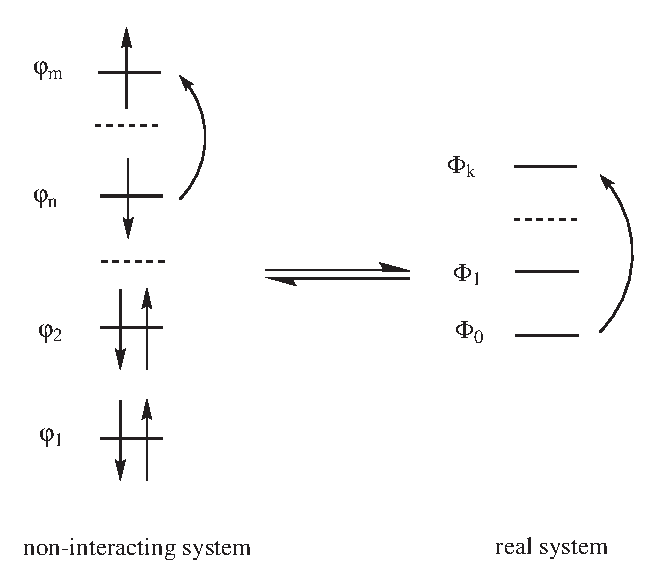
\includegraphics[scale=0.7]{TDexcitation.eps}
\caption{one to one correspondence  of electron excitation tween
non-interacting system and real system}\label{TDDFT:2}
\end{center}
\end{figure}



%%%%%%%%%%%%%%%%%%%%%%%%%%%%%%%%%%%%%%%%%%%%%%%%%%%%%%%%%%%%%%%%%%%%%%
\section{Linear response equation based on density matrix}
%
%
%
%
Now let's follow Casida's derivation for the linear response equation
on density matrix\footnote{see the reference of \cite{Casida1}}.
Suggest for some ground state of $\Psi_{0}$, some time dependent
perturbation is turning on:
\begin{equation}
 \label{TDDFT_Casida:1}
\delta \hat{v} (t) = \sum_{ij\sigma} \delta
v_{ij\sigma}(t)\hat{a}^{+}_{i\sigma}\hat{a}_{j\sigma} 
\end{equation} 
Here the $\hat{a}^{+}_{i\sigma}$ and $\hat{a}_{j\sigma}$ are two
annihilation operators used in second quantization theory. They
characterize that in orbital of $i$ some particle with spin of
$\sigma$ is destroyed and in the orbital $j$ this particle is
created. the $\delta v_{ij\sigma}(t)$ is some time dependent
perturbation that cause the $i$ and $j$ to have such changes. If it
goes over all the $i$ and $j$ pairs then we can use it to represent
the whole perturbation of $\delta \hat{v} (t)$ (compared with the
ordinary notion, in second quantization method we concentrate on the
generation and destruction of the particles, which is equivalent to
the changing of position variables).

What's more, the perturbed density matrix between orbital $i$ and $j$
can be expressed as:
\begin{equation}
 \label{TDDFT_Casida:2}
\delta P_{ij\sigma} (t) =
\bra{\delta
\Psi_{0}}\hat{a}^{+}_{i\sigma}\hat{a}_{j\sigma}\ket{
\Psi_{0}} + \bra{
\Psi_{0}}\hat{a}^{+}_{i\sigma}\hat{a}_{j\sigma}\ket{\delta
\Psi_{0}}
\end{equation} 

Now both of the $\delta P_{ij\sigma} (t)$ and $\delta v_{ij\sigma}
(t)$ can be associated with each other through some general
density kernel of $\chi_{ij\sigma, kl\tau}$:
\begin{equation}
  \label{TDDFT_Casida:3}
\delta P_{ij\sigma} (t) = \sum_{kl\tau}\int \chi_{ij\sigma, kl\tau}(t
- t^{'}) \delta v_{kl\tau} (t^{'}) dt^{'}
\end{equation} 
The (\ref{TDDFT_Casida:3}) it means that if we have some perturbation
switched on between $k$ and $l$ orbitals at time $t^{'}$ then it will
also cause the changes on the $i$ and $j$ pairs at the time $t$. Then
if we want to get the $\delta P_{ij\sigma} (t)$, we have to sum over
all the $k$ and $l$ pairs and goes over all the time space.

Here the expression above is actually identical with the analysis in
(\ref{TDDFT1}), where we have introduced the expression
from (\ref{TDDFTeq:45}) to (\ref{TDDFTeq:23}). Here the most
important distinguishment is that in the second quantization
representation the density kernel is concentrated on the particles
rather than the position variables compared with the
(\ref{TDDFTeq:29}) and (\ref{TDDFTeq:23}). However,
they are identical with each other.

Based on the (\ref{TDDFT_Casida:3}), by using the Fourier
transformation, the above expression can be transformed
into frequency space:
\begin{align}
   \label{TDDFT_Casida:8}
\delta P_{ij\sigma} (\omega) &= \sum_{kl\tau} \chi_{ij\sigma,
kl\tau}(\omega) \delta v_{kl\tau} (\omega ) 
\end{align}

From perturbation treatment, we can get the $\chi$
expression in the traditional wave function method, which is
identical to the (\ref{TDDFTeq:28}):
\begin{multline}\label{TDDFT_Casida:4}
\chi_{ij\sigma, kl\sigma^{'}}(\omega) =
\lim_{\eta \rightarrow 0^{+}}\sum_{m > 0}\left\{
\frac{\bra{0}\hat{a}^{+}_{i\sigma}\hat{a}_{j\sigma^{'}}\ket{m}
      \bra{m}\hat{a}^{+}_{k\sigma}\hat{a}_{l\sigma^{'}}\ket{0}}
      {\omega - (E_{m} - E_{0})+ i\eta}
      \right. - \\
\left. 
\frac{\bra{0}\hat{a}^{+}_{k\sigma}\hat{a}_{l\sigma^{'}}\ket{m}
      \bra{m}\hat{a}^{+}_{i\sigma}\hat{a}_{j\sigma^{'}}\ket{0}}
      {\omega + (E_{m} - E_{0})+ i\eta}
\right\}
\end{multline}

for the non-interacting system, in the gound sate we have some single
particle equation:
\begin{equation}
 \label{TDDFT_Casida:5}
\hat{h}\psi_{i\sigma} = \epsilon_{i\sigma}\psi_{i\sigma}
\end{equation} 
Here $\psi_{i\sigma}$ is the Kohn-Sham orbital, and it assumes that
we use the orthogonal basis sets. Based on this special case, the
density kernel in the (\ref{TDDFT_Casida:4}) can be expressed
as:
\begin{align}
  \label{TDDFT_Casida:7}
\chi_{ij\sigma, kl\sigma^{'}}(\omega) &=
\delta_{\sigma\sigma^{'}}\delta_{ik}\delta_{jl}\frac{
f_ { j\sigma} -
f_{i\sigma}}{\omega - (\epsilon_{i\sigma} - \epsilon_{j\sigma})}
\end{align} 
The $f_{i\sigma}$ indicates the occupation number on the orbitals (so
the orbials has been classified into virtual and occupied type).

the expression in the (\ref{TDDFT_Casida:7}) combined with
(\ref{TDDFT_Casida:8}) are our foundation for further discussion. 

%%%%%%%%%%%%%%%%%%%%%%%%%%%%%%%%%%%%%%%%%%%%%%%%%%%%%%%%%%%%%%%%%%%%%
\subsection{Linear response of the density matrix}
%
%
%
%
%
Suggest that for some ground state non-interacting system some time
dependent filed is switched on, then the perturbation in first order
for the Kohn-Sham Hamiltonian can be expressed as:
\begin{equation}
 \label{TDDFT_Casida:9}
\delta v_{eff}(r,t) =  v_{ext}(r,t) + \delta v_{KS}(r,t)
\end{equation} 
Here because of the adding of external potential of $v_{ext}(r,t)$,
the ground state density will change so accordingly, the ground state
Kohn-Sham potential of $v_{KS}$ will be altered. Hence, from the
(\ref{TDDFT_Casida:8}) we can express such relation as:
\begin{align}
\label{TDDFT_Casida:10}
 \delta P_{ij\sigma} (\omega) &= \sum_{kl\tau} \chi_{ij\sigma,
kl\tau}(\omega) \delta v^{eff}_{kl\tau} (\omega ) \nonumber \\
&=
\sum_{kl\tau} 
\delta_{\sigma\tau}\delta_{ik}\delta_{jl}\frac{f_{j\sigma} -
f_{i\sigma}}{\omega - (\epsilon_{i\sigma} - \epsilon_{j\sigma})}
\delta v^{eff}_{kl\tau} (\omega ) \nonumber \\
&= \frac{f_{j\sigma} - f_{i\sigma}}{\omega - (\epsilon_{i\sigma} -
\epsilon_{j\sigma})}
\delta v^{eff}_{ij\sigma} (\omega )
\end{align} 
Here, we can see that for the $f_{j\sigma} = f_{i\sigma}$, the first
order density matrix change is zero. It implies that only the pair of
virtual-occupied orbitals are making contribution to the first order
density. The virtual-virtual pair and occupied-occupied pair are all
goes to be zero. This character is important in the following
linear response equation establishment.

On the other hand, from the above analysis we can see that $\delta
v_{KS}(\omega)$ is also dependent on the changing of density (so as
the density matrix), hence we can express such relation as:
\begin{equation}
 \label{TDDFT_Casida:11}
\delta v^{KS}_{ij\sigma} (\omega) = \sum_{kl\tau}K_{ij\sigma,
kl\tau}(\omega) \delta P_{kl\tau} (\omega) 
\end{equation}  

Let's bring the (\ref{TDDFT_Casida:11}) into the
(\ref{TDDFT_Casida:10}) so that to eliminate the $\delta
v^{KS}_{ij\sigma} (\omega)$, then we can have:
\begin{equation}
  \frac{\omega - (\epsilon_{i\sigma} -
\epsilon_{j\sigma})}{f_{j\sigma} - f_{i\sigma}}
\delta P_{ij\sigma} (\omega) = v_{ext}(\omega) +
\sum_{kl\tau}K_{ij\sigma,
kl\tau}(\omega) \delta P_{kl\tau} (\omega)
\end{equation} 
Then let's merge the density matrix together, then we have:
\begin{equation}
\begin{split}
\label{TDDFT_Casida:12}
&\sum_{kl\sigma^{'}}^{f_{j\sigma} \neq f_{i\sigma}}  
\Bigg\{
\delta_{\sigma\sigma^{'}}\delta_{ik}\delta_{jl}
\frac{
\omega - (\epsilon_{k\sigma^{'}} - \epsilon_{l\sigma^{'}})}
{f_{l\sigma^{'}} - f_{k\sigma^{'}}}
-
K_{ij\sigma,
kl\sigma^{'}}(\omega)
\Bigg\}
\delta P_{kl\sigma^{'}} (\omega) \\
&= v_{ext}(\omega)
\end{split} 
\end{equation}
Now we have arrived at some equation, this fundamental equation
associates the frequency and the density matrix together, later we
will build the real linear response equation from this point.
However, so far let's first analyze the four index variable of
$K_{ij\sigma, kl\sigma^{'}}(\omega)$ first. 


%%%%%%%%%%%%%%%%%%%%%%%%%%%%%%%%%%%%%%%%%%%%%%%%%%%%%%%%%%%%%%%%%%%%%
\subsection{The coupling matrix}
\label{sec:coupling_matrix_in_TDDFT}
%
%
%
%
%
The $K_{ij\sigma, kl\sigma^{'}}(\omega)$ appeared in the function of
(\ref{TDDFT_Casida:12}) is actually called ``coupling matrix'', which
is defined in (\ref{TDDFT_Casida:11}):
\begin{equation}
\delta v^{KS}_{ij\sigma} (\omega) = \sum_{kl\tau}K_{ij\sigma,
kl\tau}(\omega) \delta P_{kl\tau} (\omega) 
\end{equation}
Hence we can calculate it as:
\begin{equation}
 K_{ij\sigma, kl\tau}(\omega) = \frac{\partial v^{KS}_{ij\sigma}
(\omega)}{\partial P_{kl\tau} (\omega)}
\end{equation} 
By the chain rule for the partial derivative, we can get:
\begin{align}
\label{TDDFT_Casida:13}
  K_{ij\sigma, kl\tau}(\omega) &=\int^{+\infty}_{-\infty}
e^{i\omega(t-t^{'})} \frac{\partial v^{KS}_{ij\sigma}
(t)}{\partial P_{kl\tau} (t^{'})} d(t-t^{'}) \nonumber \\
&= \int^{+\infty}_{-\infty}
e^{i\omega(t-t^{'})} \Bigg\{ 
\sum_{\mu}\int 
\frac{\delta v^{KS}_{ij\sigma}(t)}
{\delta \rho_{\mu} (r^{'}, t^{''})}
\frac{\partial\rho_{\mu} (r^{'},t^{''})}{\partial P_{kl\tau} (t^{'})}
d^{3}r^{'}dt^{''}
 \Bigg\} d(t-t^{'}) \nonumber \\
&=
(\varphi^{*}_{i\sigma}\varphi_{j\sigma}|\varphi^{*}_{k\tau}\varphi_{
l\tau}) + \int^{+\infty}_{-\infty}
e^{i\omega(t-t^{'})} \nonumber \\
&\Bigg\{
\int
\varphi^{*}_{i\sigma}(r)\varphi_{j\sigma}(r)  
\frac{\delta^{2} E_{XC}}
{\delta \rho_{\sigma} (r, t)\delta \rho_{\tau} (r^{'}, t^{'})}
\varphi^{*}_{k\tau}(r^{'})\varphi_{l\tau}(r^{'})
d^{3}r^{'}d^{3}r
\Bigg\} d(t-t^{'})
\end{align}

If we apply the adiabatic approximation(see \ref{TDDFT_EXC_eq:2}),
then we can have the second term indepdent of time:
\begin{multline}
\int^{+\infty}_{-\infty}
e^{i\omega(t-t^{'})} \Bigg\{
\int
\varphi^{*}_{i\sigma}(r)\varphi_{j\sigma}(r)\\
\shoveleft{  
\frac{\delta^{2} E_{XC}}
{\delta \rho_{\sigma} (r, t)\delta \rho_{\tau} (r^{'}, t^{'})}
\varphi^{*}_{k\tau}(r^{'})\varphi_{l\tau}(r^{'})
d^{3}r^{'}d^{3}r
\Bigg\} d(t-t^{'})}  \\
= \int
\varphi^{*}_{i\sigma}(r)\varphi_{j\sigma}(r)  
\frac{\delta^{2} E_{XC}}
{\delta \rho_{\sigma} (r)\delta \rho_{\tau} (r^{'})}
\varphi^{*}_{k\tau}(r^{'})\varphi_{l\tau}(r^{'})
d^{3}r^{'}d^{3}r
\end{multline} 
This is what we have got in the previous section. Hence finally, the
coupling matrix is expressed as:
\begin{align}
\label{TDDFT_Casida:14}
 K_{ij\sigma, kl\tau}(\omega) &=
(\varphi^{*}_{i\sigma}\varphi_{j\sigma}|\varphi^{*}_{k\tau}\varphi_{
l\tau}) + \nonumber \\
&\int
\varphi^{*}_{i\sigma}(r)\varphi_{j\sigma}(r)  
\frac{\delta^{2} E_{XC}}
{\delta \rho_{\sigma} (r)\delta \rho_{\tau} (r^{'})}
\varphi^{*}_{k\tau}(r^{'})\varphi_{l\tau}(r^{'})
d^{3}r^{'}d^{3}r
\end{align}

%%%%%%%%%%%%%%%%%%%%%%%%%%%%%%%%%%%%%%%%%%%%%%%%%%%%%%%%%%%%%%%%%%%%%
\subsection{Structure for linear response equation}
\label{TDDFT:1}
%
%
%
%
%
As what has been demonstrated in the (\ref{TDDFT_Casida:10}), only
the occ-vir pair blocks exists in the expression of density matrix.
Hence for more clear specification, let's follow the convention
that the subscript of $i,j, k$ etc. indicate the occupied orbitals,
$a, b, c$ etc. represent the virtual orbitals; and $p, q, r$ etc.
refer to the general orbitals.
Based on this point, the result in the (\ref{TDDFT_Casida:12}) can be
rewritten as:
\begin{equation}
\label{TDDFT_Casida:18} 
 \begin{split}
  &\sum_{j}\sum_{b}\sum_{\sigma^{'}}\left\lbrace 
\delta_{\sigma\sigma^{'}}\delta_{ij}\delta_{ab}\left[ 
\frac{\omega - (\epsilon_{i} - \epsilon_{a})}{f_{a} -
f_{i}} \right] 
- K_{ia\sigma,
jb\sigma^{'}}(\omega)
\right\rbrace 
\delta P_{jb\sigma^{'}} (\omega) \\
&- \sum_{b}\sum_{j}\sum_{\sigma^{'}}K_{ia\sigma,
bj\sigma^{'}}(\omega)\delta P_{bj\sigma^{'}} (\omega)
= v_{ext}(\omega)
 \end{split}
\end{equation} 
this function is for some pre-determined occ-vir pair of $ia\sigma$ in
the $K_{ia\sigma, jb\sigma^{'}}$. Compared with the
(\ref{TDDFT_Casida:12}), we have such index correspondence:
\begin{align}
 i \leftrightarrow i  &\quad  j \leftrightarrow a \quad
(\text{pre-determined pairs}) \nonumber \\
 k \leftrightarrow j  &\quad  l \leftrightarrow b \quad
(\text{the first term}) \nonumber \\
 k \leftrightarrow b  &\quad  l \leftrightarrow j \quad
(\text{the second term}) \nonumber \\
\end{align} 

However, for the pre-determined pair of $ai\sigma$, we can have some
conjugated equation (derived in the same way):
\begin{equation}
\label{TDDFT_Casida:19} 
  \begin{split}
  &\sum_{b}\sum_{j}\sum_{\sigma^{'}}\left\lbrace 
\delta_{\sigma\sigma^{'}}\delta_{ij}\delta_{ab}\left[ 
\frac{\omega - (\epsilon_{a} - \epsilon_{i})}{f_{i} -
f_{a}} \right] 
- K_{ai\sigma,
bj\sigma^{'}}(\omega)
\right\rbrace 
\delta P_{bj\sigma^{'}} (\omega) \\
&- \sum_{j}\sum_{b}\sum_{\sigma^{'}}K_{ai\sigma,
jb\sigma^{'}}(\omega)\delta P_{jb\sigma^{'}} (\omega)
= v_{ext}(\omega)
 \end{split}
\end{equation} 

Now let's try to combine them together to form the final equation.
Firstly, we notice that (this is obvious from the definition of
density matrix): 
\begin{equation}
\label{TDDFT_Casida:16}
 \delta P_{jb\sigma^{'}} (\omega) = \delta P^{*}_{bj\sigma^{'}}
(\omega)
\end{equation}
Moreover, let's deal with the left side of matrix element:
\begin{equation}
\label{TDDFT_Casida:17} 
\begin{split}
 A_{ia\sigma, jb\sigma^{'}} &=
\delta_{\sigma\sigma^{'}}\delta_{ij}\delta_{ab}\left[ 
\frac{(\epsilon_{i} - \epsilon_{a})}{f_{a} -
f_{i}} \right] 
+ K_{ia\sigma, jb\sigma^{'}}(\omega) \\
&=\delta_{\sigma\sigma^{'}}\delta_{ij}\delta_{ab}(\epsilon_{a} -
\epsilon_{i}) + K_{ia\sigma, jb\sigma^{'}}(\omega) 
\end{split}
\end{equation}  
Here we have to remember that $f_{a} = 0$ and $f_{i} = 1$.
Hence the first equation in (\ref{TDDFT_Casida:18}) is
converted to be:
\begin{equation}
 \label{TDDFT_Casida:20}
-\omega \delta P_{ia\sigma} (\omega) - v_{ext}(\omega) = 
\sum_{j}\sum_{b}\sum_{\sigma^{'}}A_{ai\sigma, jb\sigma^{'}}\delta
P_{jb\sigma^{'}}
(\omega) + K_{ai\sigma, bj\sigma^{'}}\delta P_{bj\sigma^{'}}(\omega)
\end{equation} 

The conjugatedequation can be rewriten as:
\begin{equation}
 \label{TDDFT_Casida:21}
\omega \delta P_{ai\sigma} (\omega) - v_{ext}(\omega) = 
\sum_{j}\sum_{b}\sum_{\sigma^{'}}A_{ia\sigma, jb\sigma^{'}}\delta
P_{jb\sigma^{'}}
(\omega) + K_{ia\sigma, bj\sigma^{'}}\delta P_{bj\sigma^{'}}(\omega)
\end{equation} 

Finally, let's introduce the ``zero frequency limit'' which is
usually used in deriving the final equation; that is to say,
$v_{ext}(\omega)$ can be set to $0$. Thus we can set the
$v_{ext}(\omega)$ into zero. Hence the final linear equation is:
\begin{equation}
 \label{TDDFT_Casida_final:1}
-\omega \delta P_{ia\sigma} (\omega)  = 
\sum_{j}\sum_{b}\sum_{\sigma^{'}}A_{ai\sigma, jb\sigma^{'}}\delta
P_{jb\sigma^{'}}
(\omega) + K_{ai\sigma, bj\sigma^{'}}\delta P_{bj\sigma^{'}}(\omega)
\end{equation} 

The conjugatedequation can be rewriten as:
\begin{equation}
 \label{TDDFT_Casida_final:2}
\omega \delta P_{ai\sigma} (\omega)  = 
\sum_{j}\sum_{b}\sum_{\sigma^{'}}A_{ia\sigma, jb\sigma^{'}}\delta
P_{jb\sigma^{'}}
(\omega) + K_{ia\sigma, bj\sigma^{'}}\delta P_{bj\sigma^{'}}(\omega)
\end{equation} 
They are same with the equations we got in the
(\ref{TTDFT_ENERGY_TFLRE}).


%%%%%%%%%%%%%%%%%%%%%%%%%%%%%%%%%%%%%%%%%%%%%%%%%%%%%%%%%%%%%%%%%%%%%%
\section{Gordon's way to derive the linear response equation}
%
%
%
%
In the previous content, we have presented two ways to derive to
linear response equation, both of them are given in the complete and
detailed way. However, the two above derivations share a same
character, that is they are all based upon the perturbation on KS
orbitals. Their difference, is that the Gross's derivation is based
on the electron density (so we use the functional and functional
derivatives to connect the perturbed density, Hamiltonian etc.), but
Cacida use the density matrix to rewrite the whole expression (hence
the expression is based on the annihilation operator, so we get
different expression for the density response kernel). However, the
physical idea is same among the two way of derivations. However, all
of them are based on the MO representation, that's what they share in
common.

Now in this section we will present the third way to derive the
linear response equation\cite{Gordon, Hirata1999291}. The derivation
here is totally based on the perturbation of Fock matrix, rather
than the MO space-this is the essential distinguishment between this
method and the above methods. However, as what has been demonstrated;
the physical idea is shared between all of them.

%%%%%%%%%%%%%%%%%%%%%%%%%%%%%%%%%%%%%%%%%%%%%%%%%%%%%%%%%%%%%%%%%%%%%%
\subsection{Starting from TDKS equation}\label{Gordon_TDKS}
%
%
%
%
Let's from the matrix form of TDKS (time dependent Kohn-Sham)
equation, which has been discussed in detail at the section
\ref{TDKS_equation}. We are starting from the equation
(\ref{TDDFTeq:21}):
\begin{equation}\label{Grodon_TDDFT_equation:1}
i \frac{\partial P_{pr}}{\partial t} =
\sum_{q}\left\{F_{pq}P_{qr} -
P_{pq}F_{qr}\right\}
\end{equation}
Here the $P_{pq}$ is the density matrix between the basis set
functions of $\psi_{p}(r)$ and $\psi_{q}(r)$:
\begin{equation}
 \label{Grodon_TDDFT_equation:2}
\rho(r) = \sum_{pq}P_{pq}\psi^{*}_{p}(r)\psi_{q}(r)
\end{equation} 
Here the basis set function is the KS orbital describing the ground
state of the system.

On the other hand, the $F_{pq}$ is the Fock matrix for the basis set
functions and the time-dependent Kohn-sham Hamiltonian (as defined
in the \ref{TDDFTeq:17}):
\begin{multline}
\label{Grodon_TDDFT_equation:3}
F_{pq} = 
\int d^{3}r\psi^{*}_{p}(r)\left\{ -\frac{1}{2}\nabla^{2} + v(r,t) +
\int d^{3}r^{'}\frac{\rho(r^{'}, t)}{|r-r^{'}|} \right. \\
\left. + \frac{\delta
E_{xc}[\rho(r,t)]}{\delta\rho(r,t)} \right\}\psi_{q}(r)
\end{multline}

Generally, as what we have always followed; to directly solve this
equation is very hard; hence we employ the perturbation treatment.
let's start from the ground state, since the Kohn-sham orbital are
all orthogonal with each other, we can have:
\begin{align}
 \label{Grodon_TDDFT_equation:4}
P^{0}_{pq} &= \delta_{pq} \nonumber \\
F^{0}_{pq} &= \epsilon_{q}\delta_{pq} 
\end{align}
Different with the (\ref{Grodon_TDDFT_equation:3}), the $F^{0}_{pq}$
here is only referred as the ground state Kohn-Sham Hamiltonian:
\begin{align}\label{Grodon_TDDFT_equation:12}
F^{0}_{pq} &= 
\int d^{3}r\psi^{*}_{p}(r)\left\{ -\frac{1}{2}\nabla^{2} +
\int d^{3}r^{'}\frac{\rho(r^{'}, t)}{|r-r^{'}|}  + \frac{\delta
E_{xc}}{\delta\rho(r)} \right\}\psi_{q}(r) \nonumber \\
&=\int d^{3}r\psi^{*}_{p}(r) F^{KS}\psi_{q}(r) \nonumber \\
&=\epsilon_{q}\int d^{3}r\psi^{*}_{p}(r)\psi_{q}(r) \nonumber \\
&=\epsilon_{q}\delta_{pq}
\end{align}
$\epsilon_{q}$ here is the orbital energy for the orbital $q$.

Now let's introduce the naming of the subscript, we use $p,q,r\cdots$
to designate the general orbitals, $i,j,k\cdots$ to denote the
occupied orbitals and $a,b,c\cdots$ to refer to the virtual orbitals.

For the ground state, since the density matrix of $P$ is invarient of
time change, then the equation (\ref{Grodon_TDDFT_equation:1})
becomes:
\begin{equation}\label{Grodon_TDDFT_equation:5}
\sum_{q}\left\{F^{0}_{pq}P^{0}_{qr} -
P^{0}_{pq}F^{0}_{qr}\right\} = 0
\end{equation}

Now suggest that some oscillatory perturbation is switched on (such
as the case in photochemistry), the external field can be expressed
as:
\begin{equation}\label{Grodon_TDDFT_equation:6}
v_{1}(r,t) = \frac{1}{2}\left[ f_{pq}e^{i\omega t} + f_{qp}e^{-i\omega
t}\right] 
\end{equation}
Here we have $f_{qp} = f^{*}_{pq}$ so that to ensure that the
perturbation operator is hermitian. Furthermore, we note that this
expression actually is consistent with the form in
(\ref{TDDFTeq:51}), we only extend the $E$ there as the $f_{pq}$ and
$f_{qp}$.

As the perturbation is switched on, then the density matrix of $P$ is
also changed:
\begin{equation}\label{Grodon_TDDFT_equation:7}
P_{pq} = P^{0}_{pq} + P^{1}_{pq}
\end{equation}
the $P^{1}_{pq}$ could be expressed as:
\begin{equation}\label{Grodon_TDDFT_equation:8}
P^{1}_{pq} = \frac{1}{2}\left[ d_{pq}e^{i\omega t} + d_{qp}e^{-i\omega
t}\right] 
\end{equation}

For the Fock matrix, the corresponding change can be expressed as:
\begin{equation}\label{Grodon_TDDFT_equation:9}
F_{pq} = F^{0}_{pq} + G_{pq} + F^{1}_{pq}
\end{equation}
$G_{pq}$ is referred as the Fock matrix for the $v_{1}(r,t)$:
\begin{equation}
\label{Grodon_TDDFT_equation:10}
G_{pq} = \int d^{3}r v_{1}(r,t)\psi^{*}_{p}(r)\psi_{q}(r)
\end{equation} 
and $F^{1}_{pq}$ could be expressed as:
\begin{equation}\label{Grodon_TDDFT_equation:11}
F^{1}_{pq} = \sum_{rs}\frac{\partial F_{pq}}{\partial
P_{rs}}P^{1}_{rs} 
\end{equation}

The expression in (\ref{Grodon_TDDFT_equation:9}) actually can be
easily understood. Suggest we have some function of $f(x)$, then the
differential of $f(x)$ is:
\begin{equation}
 df(x) = f'(x)dx
\end{equation}
Hence the $f(x) + df(x)$ just corresponds the little change for
$f(x)$ at the certian point of $x$, thus we can have the
similarities:
\begin{align}
 f(x) + df(x) &\leftrightarrow F_{pq} \nonumber \\
        df(x) &\leftrightarrow F^{1}_{pq} \nonumber \\
        f'(x) &\leftrightarrow \frac{\partial F_{pq}}
                                {\partial P_{rs}} \nonumber \\
        dx &\leftrightarrow  P^{1}_{rs}
\end{align}
Certainly we have to remember here that the Fock matrix is the
multivariate function for density matrix.

%%%%%%%%%%%%%%%%%%%%%%%%%%%%%%%%%%%%%%%%%%%%%%%%%%%%%%%%%%%%%%%%%%%%%%
\subsection{Further discussion for $F^{1}_{pq}$}
%
%
%
%
%
Now let's stop for a little while and go to see the details for the
$F^{1}_{pq}$, the problem is; whether this express can correspond to
the coupling matrix (Actually, judging from the appearance, it
should be)?

Let's suggest that the exchange correlation energy can be expressed
as:
\begin{equation}
 E_{XC} = \int L(r) d^{3}r
\end{equation}
Then the Fock matrix expressed in the
(\ref{Grodon_TDDFT_equation:12}) is actually:
\begin{equation}
\label{Grodon_TDDFT_equation:13}
 F^{0}_{pq} = \int d^{3}r\int d^{3}r^{'}\psi^{*}_{p}(r)
\frac{\rho(r^{'})}{|r-r^{'}|}
\psi_{q}(r) + \int d^{3}r
v_{xc}(r)\psi^{*}_{p}(r)\psi_{q}(r)
\end{equation} 
Hence we can get:
\begin{align}
 \label{Grodon_TDDFT_equation:14}
\frac{\partial F_{pq}}{\partial
P_{rs}}
&= \int d^{3}r\int d^{3}r^{'}\psi^{*}_{p}(r)\frac{\partial\left( 
\frac{\rho(r^{'})}{|r-r^{'}|}\right) }{\partial P_{st}}
\psi_{q}(r) + \int d^{3}r
\frac{\partial v_{xc}(r)}{\partial P_{st}}\psi^{*}_{p}(r)\psi_{q}(r)
\nonumber \\
&= \int d^{3}r\int d^{3}r^{'}
\psi^{*}_{s}(r^{'})\psi_{t}(r^{'})
\frac{1}{|r-r^{'}|}
\psi^{*}_{p}(r)\psi_{q}(r) \nonumber \\
&+
\int d^{3}r\int d^{3}r^{'}
\frac{\delta v_{xc}(r)}{\delta \rho(r^{'})}\frac{\partial
\rho(r^{'})}{\partial P_{st}}\psi^{*}_{p}(r)\psi_{q}(r)
\nonumber \\
&= (\psi_{p}\psi_{q}|\psi_{s}\psi_{t}) + \int d^{3}r\int d^{3}r^{'}
\psi^{*}_{p}(r)\psi_{q}(r)
\frac{\delta^{2} L (r)}{\delta \rho(r)\delta
\rho(r^{'})}\psi^{*}_{s}(r)\psi_{t}(r)
\end{align}
Now compared with the coupling matrix in the secion 
\ref{sec:coupling_matrix_in_TDDFT}, this is just the $K_{pq,st}$. The
only thing is that we have not taken spin into account.

%%%%%%%%%%%%%%%%%%%%%%%%%%%%%%%%%%%%%%%%%%%%%%%%%%%%%%%%%%%%%%%%%%%%%%
\subsection{Spin consideration}
%
%
%
Now let's take spin into consideration. Since for the ground state KS
equation, the $P^{0}_{pq}$ and $F^{0}_{pq}$ are all for pure spin
state:
\begin{align}
  \label{Grodon_TDDFT_equation:15}
P^{0}_{p\sigma,q\tau} &= \delta_{\sigma\tau}\delta_{pq} \nonumber \\
F^{0}_{p\sigma,q\tau} &= \epsilon_{q}\delta_{\sigma\tau}\delta_{pq}
\end{align}
Hence we can label them as $P^{0}_{pq\sigma}$ and $F^{0}_{pq\sigma}$.

For the $F^{1}_{pq}$, the response for the density matrix should take
into both of the spin states, so that it gives:
\begin{align}
   \label{Grodon_TDDFT_equation:16}
F^{1}_{pq\sigma} = \sum_{\tau}\sum_{rs}\frac{\partial
F^{0}_{pq\sigma}}{\partial
P_{rs\tau}}P^{1}_{rs\tau} 
\end{align}
And for the $P^{1}_{pq}$, as for well known fact that it only exists
for the occupied-virtual blocks and it's also the pure spin state:
\begin{equation}
  \label{Grodon_TDDFT_equation:17}
P^{1}_{pq\sigma} = 
\begin{cases}
0 & p=i, q= j \\
0 & p=a, q= b \\
\neq 0 & p=a, q = i \quad \text{or} \quad p = j, q = b              
\end{cases}
\end{equation} 

%%%%%%%%%%%%%%%%%%%%%%%%%%%%%%%%%%%%%%%%%%%%%%%%%%%%%%%%%%%%%%%%%%%%%%
\subsection{Linear response equation}
%
%
%
Finally, let's bring the (\ref{Grodon_TDDFT_equation:15}),
(\ref{Grodon_TDDFT_equation:16}) and 
(\ref{Grodon_TDDFT_equation:17}) as well as the corresponding
expression in section \ref{Gordon_TDKS} all into the equation
(\ref{Grodon_TDDFT_equation:1}), by collecting the terms multiplying
$e^{i\omega t}$ together, we can get some equation:
\begin{align}
 \label{Grodon_TDDFT_equation:18}
&F_{aa\sigma}P_{ai\sigma} - P_{ai\sigma}F_{ii\sigma} + \left\lbrace 
\sum_{st\tau}\left[\frac{\partial
F^{0}_{ai\sigma}}{\partial
P_{bj\tau}}P_{bj\tau} + \frac{\partial
F^{0}_{ai\sigma}}{\partial
P_{jb\tau}}P_{jb\tau} \right] 
+ g_{ai} \right\rbrace P^{0}_{ii\sigma} \nonumber \\
&=\omega P_{ai\sigma}
\end{align}

This function can be further simplified as:
\begin{align}
 \label{Grodon_TDDFT_equation:19}
&\left\lbrace 
\sum_{st\tau}\left[(\epsilon_{b} -
\epsilon_{j})
\delta_{ab}\delta_{ij}\delta_{\sigma\tau}P_{bj\tau} +
\frac{\partial
F^{0}_{ai\sigma}}{\partial
P_{bj\tau}}P_{bj\tau} + \frac{\partial
F^{0}_{ai\sigma}}{\partial
P_{jb\tau}}P_{jb\tau} \right] 
+ g_{ai} \right\rbrace \nonumber \\
&=\omega P_{ai\sigma}
\end{align}

By colleting the terms multiplying with $e^{-i\omega t}$, we can get
its pair equation:
\begin{align}
 \label{Grodon_TDDFT_equation:19}
&\left\lbrace 
\sum_{st\tau}\left[(\epsilon_{b} -
\epsilon_{j})
\delta_{ab}\delta_{ij}\delta_{\sigma\tau}P_{jb\tau} +
\frac{\partial
F^{0}_{ia\sigma}}{\partial
P_{bj\tau}}P_{bj\tau} + \frac{\partial
F^{0}_{ia\sigma}}{\partial
P_{jb\tau}}P_{jb\tau} \right] 
+ g_{ia} \right\rbrace \nonumber \\
&=-\omega P_{ia\sigma}
\end{align}

by neglecting the $g_{ia}$ and $g_{ai}$ at the zero frequency limit,
we can see the pair of equations are same with the final equations we
get in section (\ref{TTDFT_ENERGY_TFLRE}).

%%%%%%%%%%%%%%%%%%%%%%%%%%%%%%%%%%%%%%%%%%%%%%%%%%%%%%%%%%%%%%%%%%%%%%
\section{Singlet and triplet states}
%
%
%
Now let's made further discussion in terms of the spin. For the close
shell molecule its singlet and triplet excitation
can be expressed based on the density
matrix\cite{Bauernschmitt1996454}:
\begin{align}
 \label{TDDFT_singlet_triplet:0}
P_{ais} &= \frac{1}{\sqrt{2}}(P_{ai\alpha} + P_{ai\beta}) \nonumber \\
P_{ait} &= \frac{1}{\sqrt{2}}(P_{ai\alpha} - P_{ai\beta})
\end{align}
Here, ``s'' denotes the siglet state, and ``t'' is short for the
triplet state\footnote{For the origin of the singlet and triplet in
the TDDFT, please see the paper \cite{Gross8}. However, we should
note that there's no rigorous explanation for its origin}.
let's go to derive the concrete expression in terms of the spin state.

First of all, the general linear response equations are defined in
the (\ref{TDDFT_Casida_final:1}) and (\ref{TDDFT_Casida_final:2}),
which takes the form that:
\begin{equation}
 \label{TDDFT_singlet_triplet:1}
-\omega  P_{ia\alpha} (\omega)  = 
\sum_{j}\sum_{b}\sum_{\sigma}\left\lbrace A_{ai\alpha, jb\sigma}
P_{jb\sigma}
(\omega) + K_{ai\alpha, bj\sigma}
P_{bj\sigma}(\omega)\right\rbrace 
\end{equation}
and
\begin{equation}
 \label{TDDFT_singlet_triplet:2}
-\omega  P_{ia\beta} (\omega)  = 
\sum_{j}\sum_{b}\sum_{\sigma}\left\lbrace A_{ai\beta, jb\sigma}
P_{jb\sigma}
(\omega) + K_{ai\beta, bj\sigma}
P_{bj\sigma}(\omega)\right\rbrace 
\end{equation}

The corresponding pair equations are:
\begin{equation}
 \label{TDDFT_singlet_triplet:3}
\omega P_{ai\alpha} (\omega)  = 
\sum_{j}\sum_{b}\sum_{\sigma}A_{ia\alpha, jb\sigma}
P_{jb\sigma}(\omega) + K_{ia\alpha, bj\sigma}
P_{bj\sigma}(\omega)
\end{equation} 
and 
\begin{equation}
 \label{TDDFT_singlet_triplet:4}
\omega P_{ai\beta} (\omega)  = 
\sum_{j}\sum_{b}\sum_{\sigma}A_{ia\beta, jb\sigma}
P_{jb\sigma}(\omega) + K_{ia\beta, bj\sigma}
P_{bj\sigma}(\omega)
\end{equation} 

We starts from the two pair equations. Among them, the 
coupling matrix $K$ is defined as:
\begin{align}
\label{TDDFT_singlet_triplet:5}
 K_{ai\sigma, bj\tau}(\omega) &=
(\varphi^{*}_{a\sigma}\varphi_{i\sigma}|\varphi^{*}_{b\tau}\varphi_{
j\tau}) + \nonumber \\
&\int
\varphi^{*}_{a\sigma}(r)\varphi_{i\sigma}(r)  
\frac{\delta^{2} E_{XC}}
{\delta \rho_{\sigma} (r)\delta \rho_{\tau} (r^{'})}
\varphi^{*}_{b\tau}(r^{'})\varphi_{j\tau}(r^{'})
d^{3}r^{'}d^{3}r \nonumber \\
&=(ai|bj) + (ai|E^{XC}_{\sigma\tau}|bj)      
\end{align}
and the corresponding $A$ is:
\begin{equation}
\label{TDDFT_singlet_triplet:6}
 A_{ia\sigma, jb\sigma^{'}} 
=\delta_{\sigma\sigma^{'}}\delta_{ij}\delta_{ab}(\epsilon_{b} -
\epsilon_{j}) + K_{ia\sigma, jb\sigma^{'}}(\omega)
\end{equation}  

%%%%%%%%%%%%%%%%%%%%%%%%%%%%%%%%%%%%%%%%%%%%%%%%%%%%%%%%%%%%%%%%%%%%%%
\subsection{Properties for the coupling matrix}
%
%
%
%
Before we proceed on it's better for us to discuss a little bit more
about the prperties for the coupling matrix in terms of the spin
state.

As we have known, the coulomb matrix is invariant of the spin state.
For the exchange correlation part, since the second functional
derivatives is exchangeable:
\begin{equation}
\begin{split}
&\int
\varphi^{*}_{a\sigma}(r)\varphi_{i\sigma}(r)  
\frac{\delta^{2} E_{XC}}
{\delta \rho_{\sigma} (r)\delta \rho_{\tau} (r^{'})}
\varphi^{*}_{b\tau}(r^{'})\varphi_{j\tau}(r^{'})
d^{3}r^{'}d^{3}r \\
&= \int
\varphi^{*}_{a\sigma}(r)\varphi_{i\sigma}(r)  
\frac{\delta^{2} E_{XC}}
{\delta \rho_{\tau} (r^{'})\delta \rho_{\sigma} (r)}
\varphi^{*}_{b\tau}(r^{'})\varphi_{j\tau}(r^{'})
d^{3}r^{'}d^{3}r                 
\end{split}
\end{equation}  
Hence it's easily turned out that:
\begin{equation}
 (ai|E^{XC}_{\sigma\tau}|bj)   = 
(ai|E^{XC}_{\tau\sigma}|bj) = 
(ia|E^{XC}_{\sigma\tau}|bj) =
(ai|E^{XC}_{\sigma\tau}|jb) = 
(bj|E^{XC}_{\sigma\tau}|ai)      
\end{equation}
This property brings great feasibility for transforming the coupling
matrix. Hence finally, for the coupling matrix, we have:
\begin{equation}
\label{TDDFT_singlet_triplet:7}
K_{ai\sigma, bj\tau} = K_{bj\tau, ai\sigma}
= K_{ia\sigma, bj\tau} = K_{ai\sigma, jb\tau}
\end{equation}
 
For the matrix of $A$, compared with $K$ it's only have a redundant
term of $\delta_{\sigma\sigma^{'}}\delta_{ij}\delta_{ab}(\epsilon_{b}
-\epsilon_{j})$. However, we can see that this term is diagonal for
the block of $ai, bj$. Hence for the $A$ matrix we also have the
above equality\footnote{Here we have not considered the hybird
functional situation which requires the additional exchange term.
However, we can only merely add it in and it does not affect the
discussion here}:
\begin{equation}
\label{TDDFT_singlet_triplet:8}
A_{ai\sigma, bj\tau} = A_{bj\tau, ai\sigma}
= A_{ia\sigma, bj\tau} = A_{ai\sigma, jb\tau}
\end{equation}

%%%%%%%%%%%%%%%%%%%%%%%%%%%%%%%%%%%%%%%%%%%%%%%%%%%%%%%%%%%%%%%%%%%%%%
\subsection{Final expression}
%
%
%
%
Now according to the definition in (\ref{TDDFT_singlet_triplet:0}),
we can add (\ref{TDDFT_singlet_triplet:1}) and
(\ref{TDDFT_singlet_triplet:2}) together and multiply factor
$\frac{1}{\sqrt{2}}$ to each side, then we can get:
\begin{equation}
 \begin{split}
&-\omega  P_{ias} (\omega) \\
&=
\frac{1}{\sqrt{2}}\sum_{j}\sum_{b}\Big\{ \left[ 
\left( A_{ai\alpha, jb\alpha} + A_{ai\beta,
jb\alpha}\right)P_{jb\alpha} + 
\left( K_{ai\alpha, bj\alpha} +
K_{ai\beta, bj\alpha}\right)P_{bj\alpha} \right] + \\
&\left[ \left( A_{ai\alpha, jb\beta} + A_{ai\beta,
jb\beta}\right)P_{jb\beta}  +
\left( K_{ai\alpha, bj\beta} +
K_{ai\beta, bj\beta}\right)P_{bj\beta} \right] \Big\} 
 \end{split}
\label{TDDFT_singlet_triplet:9}
\end{equation} 

Now let's use the relation in (\ref{TDDFT_singlet_triplet:7}) and
(\ref{TDDFT_singlet_triplet:8}), this equality can be further
transformed as:
\begin{equation}
 \begin{split}
&-\omega  P_{ias} (\omega) \\
&=
\frac{1}{\sqrt{2}}\sum_{j}\sum_{b}\Big\{ \left[ 
\left( A_{ai\alpha, jb\alpha} + A_{ai\beta,
jb\alpha}\right)P_{jb\alpha} + 
\left( K_{ai\alpha, bj\alpha} +
K_{ai\beta, bj\alpha}\right)P_{bj\alpha} \right] + \\
&\left[ \left( A_{ai\alpha, jb\beta} + A_{ai\beta,
jb\beta}\right)P_{jb\beta}  +
\left( K_{ai\alpha, bj\beta} +
K_{ai\beta, bj\beta}\right)P_{bj\beta} \right] \Big\} 
 \end{split}
\label{TDDFT_singlet_triplet:10}
\end{equation} 


Firstly, we can use the spin symbol to specify the matrix function,
hence the function in (\ref{TDDFT_Casida_final:5}) is split into pair:
\begin{equation}\label{TDDFT_Casida_final:6}
\omega^{2} Z_{ai\alpha} 
= \sum_{j}\sum_{b}\sum_{\sigma}M_{ia\alpha, jb\sigma} Z_{bj\sigma}
\end{equation}
\begin{equation}\label{TDDFT_Casida_final:7}
\omega^{2} Z_{ai\beta} 
= \sum_{j}\sum_{b}\sum_{\sigma}M_{ia\beta, jb\sigma} Z_{bj\sigma}
\end{equation}
Here $\sigma$ goes over all the spin states, including the $\alpha$ and
$\beta$. 

Now let's multiply each of the equation with $(\sqrt{2})^{-1}$ and add
them together:
\begin{align}
 \omega^{2} \frac{1}{\sqrt{2}}(Z_{ai\alpha} + Z_{ai\beta})
&= \sum_{j}\sum_{b}\frac{1}{\sqrt{2}}(Z_{ai\alpha} +
Z_{ai\beta}) (M_{ia\alpha, jb\alpha} + M_{ia\alpha, jb\beta}\nonumber \\
& +M_{ia\beta, jb\alpha} +M_{ia\beta, jb\beta} ) \Rightarrow \nonumber
\\
\omega^{2} Z_{ais} &= \sum_{j}\sum_{b} Z_{bjs} (M_{ia\alpha, jb\alpha} +
M_{ia\alpha, jb\beta} +M_{ia\beta, jb\alpha} +M_{ia\beta, jb\beta} )
\end{align} 
In the siglet, since the $\rho_{\alpha} = \rho_{\beta}$, then we can
see that for the coupling matrix $K_{ia\sigma,
jb\sigma^{'}}(\omega)$, it has:
\begin{equation*}
 K_{ia\alpha, jb\beta}(\omega) = K_{ia\beta, jb\alpha}(\omega) \quad 
 K_{ia\alpha, jb\alpha}(\omega) = K_{ia\beta, jb\beta}(\omega)
\end{equation*}
for the term of
$\delta_{ij}\delta_{ab}\delta_{\sigma\sigma^{'}}(\epsilon_{a} -
\epsilon_{i})^{2}$, it's easily seen that this term cancelled in the
$\alpha$ and $\beta$ mixing case, and euqal to each other between the
$\alpha, \alpha$ and $\beta, \beta$ case. Hence we have the M matrix
element finally as:
\begin{multline}
 M_{ia\alpha, jb\alpha} +
M_{ia\alpha, jb\beta} +M_{ia\beta, jb\alpha} +M_{ia\beta, jb\beta} \\
= 
2\delta_{ij}\delta_{ab}(\epsilon_{a} - \epsilon_{i})^{2} + 
2(\epsilon_{a} - \epsilon_{i})^{\frac{1}{2}} 
(K_{ia\alpha, jb\alpha}(\omega) +
K_{ia\alpha, jb\beta}(\omega))(\epsilon_{b} -
\epsilon_{j})^{\frac{1}{2}}
\end{multline} 
The final matrix equation for the singlet is:
\begin{equation}
  \omega^{2}Z^{s} = M^{s}Z^{s}
\end{equation} 
With the element in $M^{s}$ is:
\begin{multline}
 M^{s}_{ia,jb} = 2\delta_{ij}\delta_{ab}(\epsilon_{a} -
\epsilon_{i})^{2} \\
+ (\epsilon_{a} - \epsilon_{i})^{\frac{1}{2}} 
(4(ia|jb) +2(ia|E^{\alpha\alpha}_{XC}|jb) + 
2(ia|E^{\alpha\beta}_{XC}|jb))(\epsilon_{b} -
\epsilon_{j})^{\frac{1}{2}}
\end{multline}

Simiarly, we can repeat the above procedure so that to produce the
triplet state (all the analysis are kept to be same, only pay attention
to the symbol change so some terms cancelled in the final expression):
\begin{equation}
  \omega^{2}Z^{t} = M^{t}Z^{t}
\end{equation} 
With the element in $M^{t}$ is:
\begin{equation}
 M^{t}_{ia,jb} = 2(\epsilon_{a} - \epsilon_{i})^{\frac{1}{2}} 
((ia|E^{\alpha\alpha}_{XC}|jb) - 
(ia|E^{\beta\beta}_{XC}|jb))(\epsilon_{b} -
\epsilon_{j})^{\frac{1}{2}}
\end{equation}




%%%%%%%%%%%%%%%%%%%%%%%%%%%%%%%%%%%%%%%%%%%%%%%%%%%%%%%%%%%%%%%%%%%%%%
\begin{comment}
%%%%%%%%%%%%%%%%%%%%%%%%%%%%%%%%%%%%%%%%%%%%%%%%%%%%%%%%%%%%%%%%%%%%%%



As what we have understand, the Fock matrix can be associated with
the functional potential:
\begin{align}
\label{TDDFT_TRANSFORMATION_EXC_KERNEL:1}
F^{\sigma}_{\mu\nu} &= \frac{\partial E^{\sigma}_{XC}}{\partial
P^{\sigma}_{\mu\nu}}
\nonumber \\
&=
\int \frac{\delta L(r)}{\delta
  \rho^{\sigma}(r)}\frac{\partial \rho^{\sigma}(r)}{\partial
P^{\sigma}_{\mu\nu}} d^{3}r
\nonumber \\
&= \int V^{\sigma}_{XC}(r) \phi^{*}_{\mu}(r)\phi_{\nu}(r) d^{3}r
\end{align}
Which is described in the (\ref{eq:XC_functional.9}). By the way, we
should remember that here the $P$ is referred to the ``density
matrix'' for the AO space not the pertubed density; for clarity, we
express the density matrix for the pertubed density as $Z$, that is
to say; $Z_{ai\sigma} = \delta P_{ai\sigma}$ in the above equations.

By the same procedure, we can evaluate the second derivatives:
\begin{align}
\label{TDDFT_TRANSFORMATION_EXC_KERNEL:2}
 \frac{\partial F^{\sigma}_{\mu\nu} }{\partial
P^{\sigma^{'}}_{\lambda\eta}} &= \int \frac{\delta 
F^{\sigma}_{\mu\nu}}
{\delta\rho_{\sigma^{'}}(r^{'})}\frac{\partial\rho_{\sigma^{'}}(r^{'})
}{
\partial
P^{\sigma^{'}}_{\lambda\eta}} d^{3}r^{'}
\nonumber \\ 
&= \int d^{3}r^{'} \frac{\delta 
F^{\sigma}_{\mu\nu}}
{\delta\rho_{\sigma^{'}}(r^{'})}\phi_{\lambda}
(r^{'})\phi_{\eta}(r^{'})
\nonumber \\ 
&= \int d^{3}r\int d^{3}r^{'}\phi^{*}_{\mu}(r)\phi_{\nu}(r)
\frac{\delta{V}^{\sigma}_{XC}(r)}{\delta\rho_{\sigma^{'}}(r^{'})}
\phi_{
\lambda} (r^{'})\phi_{\eta}(r^{'}) \nonumber \\
&= \int d^{3}r\int d^{3}r^{'}\phi^{*}_{\mu}(r)\phi_{\nu}(r)
\frac{\delta^{2}L(r)}{\delta\rho_{\sigma}(r)\delta\rho_{
\sigma^{'}}(r^{'})}
\phi_{
\lambda} (r^{'})\phi_{\eta}(r^{'})
\end{align}
The derivation here turns out that the exchange correlation kernel,
actually can be viewed as the susceptibility between the the pertubed
Fock Matrix $F_{\mu\nu}$ and pertubed $P_{\lambda\eta}$. Hence we
have: 
\begin{equation}
\begin{split}
&\sum_{ia\sigma}\sum_{kl\tau}Z_{ia\sigma}Z_{kl\tau}
\int\varphi^{*}_{i\sigma } (r)\varphi_{ j\sigma} (r) 
\frac{\delta^{2} E_{XC}}
{\delta \rho_{\sigma} (r)\delta \rho_{\tau} (r^{'})}
\varphi^{*}_{k\tau}(r^{'})\varphi_{l\tau}(r^{'})
d^{3}r^{'}d^{3}r \\
&= \sum_{\mu\nu}\sum_{\lambda\eta}\sum_{\sigma\tau}
P^{\sigma}_{\mu\nu} 
\frac{\partial F^{\sigma}_{\mu\nu}}{\partial
P^{\sigma^{'}}_{\lambda\eta}}P^{\sigma^{'}
}_{\lambda\eta} 
\end{split}
\end{equation}


Now let's go to see more details related to the final equation. The
equation shown in the (\ref{TDDFT_Casida_final:6}), actually can be
expanded as:
\begin{equation}
 \begin{split}
\omega^{2} Z_{ai\sigma} &=
\sum_{j}\sum_{b}\sum_{\sigma^{'}}M_{ia\sigma,
jb\sigma^{'}} Z_{bj\sigma^{'}}  \\
&= \sum_{jb\sigma^{'}}
\delta_{ij}\delta_{ab}\delta_{\sigma\sigma^{'}}(\epsilon_{a} -
\epsilon_{i})^{2}Z_{bj\sigma^{'}} + 2(\epsilon_{a} -
\epsilon_{i})^{\frac{1}{2}}K_{ia\sigma,
jb\sigma^{'}}(\omega)(\epsilon_{b} -
\epsilon_{j})^{\frac{1}{2}}Z_{bj\sigma^{'}} \\
&= (\epsilon_{a} -
\epsilon_{i})^{2}Z_{ai\sigma} + 2\sum_{jb\sigma^{'}}(\epsilon_{a} -
\epsilon_{i})^{\frac{1}{2}}\Big\{  (ia|jb) \\
&+(ia|E_{XC}^{\sigma\sigma^{'}}|jb) \Big\}(\epsilon_{b} -
\epsilon_{j})^{\frac{1}{2}}Z_{bj\sigma^{'}}
 \end{split}
\label{TDDFT_Casida_final:6}
\end{equation} 
Here the abbreviation is:
\begin{align}
 (ia|E^{\sigma\sigma^{'}}_{XC}|jb) &= \int d^{3}r \int d^{3}r^{'}
\varphi_{i}^{*}(r)\varphi_{a}(r)\frac{\partial^{2}
E_{XC}}{\partial \rho_{\sigma}(r)\partial \rho_{\sigma^{'}}(r^{'})}
\varphi_{j}^{*}(r^{'})\varphi_{b}(r^{'}) \nonumber \\
 (ia|jb) &= \int d^{3}r \int d^{3}r^{'} 
\varphi_{i}^{*}(r)\varphi_{a}(r) \frac{1}{r-r^{'}}
\varphi_{j}^{*}(r^{'})\varphi_{b}(r^{'}) 
\end{align}
$\varphi$ is the ground state Kohn-Sham orbitals.

Usually in practical coding, the calculation is usually transformed
back into the AO space (using the basis sets) while evaluating the
integrals, then back to the MO space (using molecular orbitals) while
forming the final matrix to calculate the linear response. Hence, how
can we transform it between the AO and MO? Let's concentrate on the
colomb integrals and the exchange-correlation integrals.

First, for the Colomb integral, it can be abbreviated as:
\begin{equation}
 J_{ia\sigma, jb\sigma^{'}} =
\sum_{jb\sigma^{'}}(ia|jb)Z_{bj\sigma^{'}}
\end{equation}  
Since the multiplier of energy differences are trivial to be added in
the final steps. For this integral, we can expand it into the AO as:
\begin{equation}
 \begin{split}
  J_{ia\sigma, jb\sigma^{'}} &=
\sum_{jb\sigma^{'}}\sum_{\mu\nu\lambda\eta}c^{*}_{i\mu}c_{a\nu}
c^{*}_{j\lambda}c_{b\eta}(\phi_{\mu}(r)\phi_{\nu}(r)|\phi_{\lambda}
(r^{'})\phi_{\eta}(r^{'}) )Z_{ bj\sigma^ {'}} \\
&=
\sum_{\mu\nu}c^{*}_{i\mu}c_{a\nu}\left\lbrace
\sum_{jb\sigma^{'}}\sum_{\lambda\eta}
c^{*}_{j\lambda}c_{b\eta}(\phi_{\mu}(r)\phi_{\nu}(r)|\phi_{\lambda}
(r^{'})\phi_{\eta}(r^{'}) )Z_{ bj\sigma^ {'}}\right\rbrace 
 \end{split}
\label{TDDFT_Casida_final:7}
\end{equation}  
Here we can see that the calculation within the curly bracket can be
calculated within the AO space. We notice that
$Z^{'}_{\lambda\eta} =
\sum_{jb\sigma^{'}}Z_{bj\sigma^{'}}c^{*}_{j\lambda}c_{b\eta}$ actually
forms some kind of new vector in the AO space. That's really what we
do
in AO calculation: first to make such transformation, then combined
with
the integral of
$(\phi_{\mu}(r)\phi_{\nu}(r)|\phi_{\lambda}(r^{'})\phi_{\eta}(r^{'}
))$
to give the result in AO space, then this result should be stored in
the $Z^{'}_{\mu\nu}$. Then we will finish the calculation in the AO
space. We note that here after the transformation of
$Z^{'}_{\lambda\eta}$, we can transform it back to the MO space by
$Z^{'}_{ai} = \sum_{\mu\nu}c^{*}_{i\mu}c_{a\nu} Z^{'}_{\mu\nu}$. Then
we
are back to the MO space and get the final result. Here the $Z^{'}$
vector is actually in dimension of $nbasis^{2}$.

Next let's talk about the the exchange-correlation part. Firstly,
let's
concentrate on the integral below:
\begin{equation}
 \begin{split}
&\sum_{jb\sigma^{'}} (ia|E_{XC}^{\sigma\sigma^{'}}|jb)
Z_{bj\sigma^{'}}
\\
&=\sum_{jb\sigma^{'}}\sum_{\mu\nu\lambda\eta}c^{*}_{i\mu}c_{a\nu}
c^{*}_{j\lambda}c_{b\eta}(\phi_{\mu}(r)\phi_{\nu}(r)|E_{XC}^{
\sigma\sigma^{'}}|\phi_{\lambda}
(r^{'})\phi_{\eta}(r^{'}) )Z_{ bj\sigma^ {'}} \\
&=\sum_{\mu\nu}c^{*}_{i\mu}c_{a\nu}\left\lbrace
\sum_{jb\sigma^{'}}\sum_{\lambda\eta}
c^{*}_{j\lambda}c_{b\eta}(\phi_{\mu}(r)\phi_{\nu}(r)|E_{XC}^{
\sigma\sigma^{'}}|\phi_{\lambda}
(r^{'})\phi_{\eta}(r^{'}) )Z_{ bj\sigma^ {'}}\right\rbrace 
 \end{split}
\label{TDDFT_Casida_final:8}
\end{equation} 
Here, we point out that the $(\phi_{\mu}(r)\phi_{\nu}(r)|E_{XC}^{
\sigma\sigma^{'}}|\phi_{\lambda} (r^{'})\phi_{\eta}(r^{'}) )$ is
actually the second partial derivatives for exchange correlation
energy with respect to the density matrix. In

Now let's combine the (\ref{TDDFT_Casida_final:8}),
(\ref{TDDFT_Casida_final:9}) and (\ref{TDDFT_Casida_final:10})
together, we can get the expression below:
\begin{equation}
 \begin{split}
  \sum_{jb\sigma^{'}} (ia|E_{XC}^{\sigma\sigma^{'}}|jb)
Z_{bj\sigma^{'}} = \sum_{\mu\nu}c^{*}_{i\mu}c_{a\nu}\left\lbrace
\sum_{jb\sigma^{'}}\sum_{\lambda\eta}
c^{*}_{j\lambda}c_{b\eta}Z_{ bj\sigma^
{'}} \frac{\partial^{2}
E_{XC}}{\partial P^{\sigma}_{\mu\nu}\partial
P^{\sigma^{'}}_{\lambda\eta}}\right\rbrace 
 \end{split}
\label{TDDFT_Casida_final:11}
\end{equation} 
Now, the same procedure can be done to the exchange correlation energy
again. Then we finish the transformation between the AO and MO.


%%%%%%%%%%%%%%%%%%%%%%%%%%%%%%%%%%%%%%%%%%%%%%%%%%%%%%%%%%%%%%%%%%%%%%
\section{Further derivation for the linear response equation}
%
%
%
%
Now let's approach to the final equation in some other
way\footnote{There seems to be something wrong with the matrix
representation, commonly used in many reference. just in the form
below:
\begin{equation}
 \omega 
\begin{bmatrix}
-1  &  0\\
 0  &  1
\end{bmatrix}
\begin{bmatrix}
  \delta P     \\
  \delta P^{*} \\
\end{bmatrix}
- v_{ext}(\omega)
= \begin{bmatrix}
  A & B \\
  B & A \\
\end{bmatrix}
\begin{bmatrix}
  \delta P     \\
  \delta P^{*} \\
\end{bmatrix} 
\end{equation} 
Here I want to mention that actually on the left side is the pure spin
state of $\delta P$, but on the right side we have added across over
all the spin states ($\sum\sigma^{'}$). So it cause some problems in
the further derivation. Hence I want to try another way to derive the
final equation. the original derivation is put into the final section
of this chapter}. 

First, we can simply add the equation in (\ref{TDDFT_Casida_final:1})
and (\ref{TDDFT_Casida_final:2}) together, which gives:
\begin{multline}
 \label{TDDFT_Casida_final:3}
\omega \left( \delta P_{ai\sigma} (\omega)-\delta P_{ia\sigma}
(\omega)\right) \\
= \sum_{j}\sum_{b}\sum_{\sigma^{'}}
\left[ ( A_{ia\sigma, jb\sigma^{'}} + B_{ia\sigma, jb\sigma^{'}})
(\delta P_{jb\sigma^{'}}(\omega) +
\delta P_{bj\sigma^{'}}(\omega))
\right] 
\end{multline}

On the other hand, we can make the (\ref{TDDFT_Casida_final:2}) and
(\ref{TDDFT_Casida_final:1}) substract each other, then it gives:
\begin{multline}
 \label{TDDFT_Casida_final:4}
\omega \left( \delta P_{ai\sigma} (\omega)+\delta P_{ia\sigma}
(\omega)\right) \\
= \sum_{j}\sum_{b}\sum_{\sigma^{'}}
\left[ ( A_{ia\sigma, jb\sigma^{'}} - B_{ia\sigma, jb\sigma^{'}})
(\delta P_{bj\sigma^{'}}(\omega) -
\delta P_{jb\sigma^{'}}(\omega))
\right] 
\end{multline}

Now let's observe the function of (\ref{TDDFT_Casida_final:4}). From
the (\ref{TDDFT_Casida:17}), we can see that 
\begin{equation*}
  A_{ia\sigma, jb\sigma^{'}} - B_{ia\sigma, jb\sigma^{'}} =
\delta_{\sigma\sigma^{'}}\delta_{ij}\delta_{ab}(\epsilon_{a} -
\epsilon_{i})
\end{equation*}
Let's bring it into the original function, it turns out:
\begin{align}
& \omega \left( \delta P_{ai\sigma} (\omega)+\delta P_{ia\sigma}
(\omega)\right) \nonumber \\
&= \sum_{j}\sum_{b}\sum_{\sigma^{'}}
\left[\delta_{\sigma\sigma^{'}}\delta_{ij}\delta_{ab}(\epsilon_{a} -
\epsilon_{i})
(\delta P_{bj\sigma^{'}}(\omega) -
\delta P_{jb\sigma^{'}}(\omega))
\right] \nonumber \\
&=  (\epsilon_{a} - \epsilon_{i}) (\delta P_{ai\sigma}(\omega) -
\delta P_{ia\sigma}(\omega))
\end{align} 
Now interestingly we can observe some very simple relationship between
the $(\delta P_{ai\sigma}(\omega) - \delta P_{ia\sigma}(\omega))$ and
the $(\delta P_{ai\sigma}(\omega) + \delta P_{ia\sigma}(\omega))$.
Here
we have such simple relation is because that the symmetrical property
of the coupling matrix. Then let's bring it back to the
(\ref{TDDFT_Casida_final:3}):
\begin{multline}
\frac{\omega^{2}}{\epsilon_{a} - \epsilon_{i}} \left( \delta
P_{ai\sigma} (\omega) + \delta P_{ia\sigma}
(\omega)\right) \\
= \sum_{j}\sum_{b}\sum_{\sigma^{'}}
\left[ ( A_{ia\sigma, jb\sigma^{'}} + B_{ia\sigma, jb\sigma^{'}})
(\delta P_{jb\sigma^{'}}(\omega) +
\delta P_{bj\sigma^{'}}(\omega))
\right] 
\end{multline} 
This is the final linear response equation. Here we can notice two
points: the first one is that the variables has been reduced into the
form of $\delta P_{ai\sigma} (\omega) + \delta P_{ia\sigma} (\omega)$.
Since $\delta P_{ai\sigma} (\omega) = \delta P^{*}_{ia\sigma}
(\omega)$, hence the index for the density matrix has been some real
number now! We have droped the complex number situation. Secondly, now
we only have one simple equation rather than a pair of equations
coupling with each other. 

Following the traditional transformation to the final function, let's
make some additional treatment. We can name some arbitrary variable of
$Z_{ai\sigma}$ as:
\begin{equation}
 Z_{ai\sigma} = \frac{1}{(\epsilon_{a} - \epsilon_{i})^{\frac{1}{2}}}
\left( \delta
P_{ai\sigma} (\omega) + \delta P_{ia\sigma}
(\omega)\right)
\end{equation} 
Hence the $\delta P_{jb\sigma^{'}}(\omega) +
\delta P_{bj\sigma^{'}}(\omega)$ on the right side of the equation can
be changed into:
\begin{equation}
 Z_{bj\sigma} = \frac{1}{(\epsilon_{b} - \epsilon_{j})^{\frac{1}{2}}}
\left( \delta P_{bj\sigma} (\omega) + \delta P_{jb\sigma}
(\omega)\right)
\end{equation}
Hence the final equation can be changed into:
\begin{equation}\label{TDDFT_Casida_final:5}
\omega^{2} Z_{ai\sigma} 
= \sum_{j}\sum_{b}\sum_{\sigma^{'}}\left[ (\epsilon_{a} -
\epsilon_{i})^{\frac{1}{2}}
 ( A_{ia\sigma, jb\sigma^{'}} + B_{ia\sigma, jb\sigma^{'}})
(\epsilon_{b} -
\epsilon_{j})^{\frac{1}{2}} \right] Z_{bj\sigma^{'}}
\end{equation}
This function just coincides with the result given in the Cacida's
paper\cite{Casida1}, although our derivation way is a bit of different
with his.

Finally let's expand the $A_{ia\sigma, jb\sigma^{'}} + B_{ia\sigma,
jb\sigma^{'}}$. It turns out that:
\begin{equation*}
A_{ia\sigma, jb\sigma^{'}} + B_{ia\sigma, jb\sigma^{'}} = 
\delta_{ij}\delta_{ab}\delta_{\sigma\sigma^{'}}(\epsilon_{a} -
\epsilon_{i}) + 2K_{ia\sigma,
jb\sigma^{'}}(\omega)
\end{equation*}
Hence the element inside the square bracket should be:
\begin{equation*}
 M_{ia\sigma, jb\sigma^{'}} =
\delta_{ij}\delta_{ab}\delta_{\sigma\sigma^{'}}(\epsilon_{a} -
\epsilon_{i})^{2} + 2(\epsilon_{a} -
\epsilon_{i})^{\frac{1}{2}}K_{ia\sigma,
jb\sigma^{'}}(\omega)(\epsilon_{b} -
\epsilon_{j})^{\frac{1}{2}}
\end{equation*} 
Hence we can introduce some new matrix of M, and obviously it's
symmetrical. Based on this new matrix, we can write the result
function
in the (\ref{TDDFT_Casida_final:5}):
\begin{equation}
\label{TDDFT_Casida_final:6}
 \omega^{2}Z = MZ
\end{equation} 
Here we should pay attention that the right side of the equation is
going over all the spin states.


%%%%%%%%%%%%%%%%%%%%%%%%%%%%%%%%%%%%%%%%%%%%%%%%%%%%%%%%%%%%%%%%%%%%%%
\section{New ways to elvaluate the exchange correlation energy in
TDDFT}
%
%
%
%
%
Firstly, we note that in reality the contribution of
exchange-correlation energy part in TDDFT is calculated in the form
of:
\begin{equation}
 \label{NEW_WAY_EXC_TDDFTeq:1}
(XC)_{pq} =
\sum_{\mu\nu\lambda\eta}t^{p}_{\mu\nu}t^{q}_{\lambda\eta}\int
\frac{\partial^{2} F(r)}{\partial P_{\mu\nu}\partial P_{\lambda\eta}}
d^{3}r
\end{equation} 
This is the matrix element expressed in the AO space, and $p$ and $q$
are the indexes of different trial densities in Davidson's method.
This expression is identical with (\ref{TDDFT_Casida_final:11}).

However, the (\ref{NEW_WAY_EXC_TDDFTeq:1}) is just unnecessarily
complicated. Which means, it has to be transformed into AO to
calculate
and then transform back to the MO space to form the final matrix.
Hence
can we find some way more efficient?

Suggest that the energy functional is general expressed as:
\begin{equation}
 F(r) =
F(\rho_{\sigma}, \nabla\rho_{\sigma}, \nabla^{2}\rho_{\sigma},
\text{etc.})
\end{equation} 
We label $\xi = \rho_{\sigma}$ or $\xi = \nabla\rho_{\sigma}$, and
consider the $\xi$ as some basic variables so that if we evaluate the
second derivatives by the $\xi$, can expression be more
computationally efficient?

The answer is definitely right. In the chapter 


%%%%%%%%%%%%%%%%%%%%%%%%%%%%%%%%%%%%%%%%%%%%%%%%%%%%%%%%%%%%%%%%%%%%%
\subsection{How to express the first order change of
density}
%
% 1  express the time dependent KS orbitals from ground states
%    coefficients are frequency dependent
% 2  to express the rho^{1}(r,t), and how to understand it
%
Now we are going to apply the matrix form of time dependent Kohn-Sham
equation to get some perturbed equation, which is similar to the from
in (\ref{TDDFTeq:32}). Before that, the first question is that how can
we express the first order of density in matrix form? 

Now let's recall the centeral algorithm for doing this. The basic idea
of the linear response equation, is to apply the perturbation theory
to the time-independent Kohn-Sham states and derive the relations
between the perturbed density and perturbed functionals. Hence,
we can expand the perturbative density on the base of the
time-independent Kohn-Sham orbitals.

For the ground state of Kohn-Sham equation, we have:
\begin{equation}\label{}
\left\{-\frac{1}{2}\nabla^{2} -v(r) + \int
d^{3}r^{'}\frac{\rho(r^{'})}{|r-r^{'}|} + \frac{\delta
E_{XC}[\rho]}{\delta \rho(r)} \right\}\chi_{q, \sigma}(r) =
\epsilon_{q}\chi_{q, \sigma}(r)
\end{equation}
Here $\epsilon_{q}$ is the energy for the KS orbital of
$\chi_{q}(r)$. Furthermore, we assume that KS orbitals are
orthogonal with each other, that is:
\begin{equation}\label{}
\int\chi_{p\sigma}(r)\chi_{q\sigma^{'}}(r)d\tau =
\delta_{pq}\delta_{\sigma\sigma^{'}}
\end{equation}
Here we note that we are following the convention that the subscript
of $i,j$ etc. indicate the occupied orbitals for Kohn-Sham time
independent states, $a, b$ etc. represent the virtual orbitals; and
$p, q$ etc. refer to the general orbitals.

Now according to the expression in (\ref{TDDFTeq:20}), the total time
dependent density is:
\begin{align}
  \label{TDDFT_Added_eq:2}
\rho(r,t) &= \sum_{j=1}^{occ}|\psi_{j}(r,t)^{2}| 
\end{align}

Based on the perturbation idea, we can also express the density as:
\begin{align}
  \label{TDDFT_Added_eq:3}
\rho(r,t) &= \rho^{ground}(r,t) + \rho^{1}(r,t) + \rho^{2}(r,t) +
\cdots
\end{align}
Here the subscript of $1, 2$ etc. represents the perturbed order. Then
by (\ref{TDDFT_Added_eq:5}), we can get:
\begin{align}
  \label{TDDFT_Added_eq:4}
  \rho(r,t) &= \sum_{p}\sum_{q}P_{pq}\chi_{p}^{*}(r)\chi_{q}(r)
  \nonumber \\
  &= \sum_{i}\sum_{j}P_{ij}\chi_{i}^{*}(r)\chi_{j}(r) +
  \sum_{i}\sum_{a}(P_{ia}\chi_{i}^{*}(r)\chi_{a}(r) + 
  P_{ai}\chi_{a}^{*}(r)\chi_{i}(r)) \nonumber \\
  &+ \sum_{a}\sum_{b}P_{ab}\chi_{a}^{*}(r)\chi_{b}(r)
\end{align}

Hence we can see that the ground state density is expressed via
the first term in the (\ref{TDDFT_Added_eq:4}), which is actually
the $\sum_{i}^{occ}P_{ii}\chi_{i}^{*}(r)\chi_{i}(r)$ due to the
non-interacting property; then the first order density is expressed
by:
\begin{equation}
  \label{TDDFT_Added_eq:6}
  \rho^{1}(r,t) = \sum_{i}\sum_{a}
\Big\{P_{ia}\chi_{i}^{*}(r)\chi_{a}(r) +
  P_{ai}\chi_{a}^{*}(r)\chi_{i}(r)\Big\}
\end{equation}
Hence it's only that the pair of virtual-occupied orbitals are making
contribution to the first order density. The virtual-virtual pair in
the
(\ref{TDDFT_Added_eq:4}) actually forms the $\rho^{2}(r,t)$, which
makes clear
physical sense.

Finally, it should note that in deriving the linear response equation,
it's in frequency space rather than the time space. Hence in the
frequency space, accordingly we have:
\begin{equation}\label{TDDFTeq:43}
\rho^{1}_{\sigma}(r,\omega) = \sum_{ia\sigma}
[P_{ia\sigma}\chi^{*}_{i,\sigma}(r)\chi_{a,\sigma}(r) +
P_{ai\sigma}\chi^{*}_{a,\sigma}(r)\chi_{i,\sigma}(r)]
\end{equation}
Here we also take spin effects into account. The $\sigma$ indicates
the spin states for the KS orbital, it can be $\alpha$ or
$\beta$. This result is also used by
Turbomole\cite{Bauernschmitt1996454}.

Furthermore, in the (\ref{TDDFTeq:43}) the $P_{ia\sigma}$ and
$P_{ai\sigma}$ are actually conjugated with  each other:
\begin{equation}
  \label{TDDFT_Added_eq:7}
P_{ia\sigma} = P_{ai\sigma}^{*}
\end{equation}

Now following the convention, we can express the first order density
into matrix form:
\begin{equation}\label{}
\begin{pmatrix}
  X \\
  Y \\
\end{pmatrix}
=|X,Y\rangle \Leftrightarrow
\begin{pmatrix}
  X_{ia\sigma} & Y_{ia\sigma} \\
\end{pmatrix}
\end{equation}
Where we have:
\begin{align}\label{}
X_{ia\sigma} &= P_{ia\sigma} \nonumber \\
Y_{ia\sigma} &= P_{ai\sigma} = X_{ia\sigma}^{*}
\end{align}
Then by each predetermined pair of orbitals $(i,a)$, we have some
vector of density matrix to correspond to it. Since the basis set
functions are fixing (they are ground state Kohn-Sham orbitals and
have been already gotten from the ground state calculation), then if
we know the density matrix vector of $|X,Y\rangle$, then we know then
first order density change so that we get the time-dependent
density. That's all what we need to do.


%%%%%%%%%%%%%%%%%%%%%%%%%%%%%%%%%%%%%%%%%%%%%%%%%%%%%%%%%%%%%%%%%%%%%%
\subsection{Matrix form of linear response equation}\label{TDDFT:3}
%
%  1 name the coupling matrix
%  2 express the density kernel of \chi_{KS} into more delicate form
%  3 express the rho^{1}
%  4 get the final equation
%  5 some physical illustration, what's the meaning of this equation
%  6 transform it into the matrix form
%
Now let's try to derive the final linear equation based on density
matrix from the result in (\ref{TDDFTeq:25}). 


Next let's consider the $\chi_{KS}$. According to the
(\ref{TDDFTeq:30}), it explicitly has the form that:
\begin{equation}
\chi_{KS,\sigma\sigma^{'}}(r,r^{'}, \omega)
=\delta(\sigma\sigma^{'})
\sum_{p}\sum_{q}(f_{p} - f_{q})* \\
\left\{\frac{\psi_{p\sigma}(r)\psi_{p\sigma^{'}}^{*}(r^{'})
\psi_{q\sigma^{'}}(r^{'})\psi_{q\sigma}^{*}(r)} {\omega -
(\epsilon_{p} - \epsilon_{q}) + i\eta} \right\}
\end{equation}
Here $p,q$ refer to the general KS orbitals. As what we have
mentioned above, it's only that $p$ and $q$ are virtual-occupied
orbital pairs that the $\chi_{KS}$ is not zero. Therefore, we can
further express the $\chi_{KS}$ as:
\begin{multline}\label{TDDFTeq:33}
\chi_{KS, \sigma\sigma^{'}}(r,r^{'}, \omega)
=\delta(\sigma\sigma^{'})\sum_{i}\sum_{a}(f_{i} - f_{a})*
\left\{\frac{\psi_{i\sigma}(r)\psi_{i\sigma^{'}}^{*}(r^{'})
\psi_{a\sigma^{'}}(r^{'})\psi_{a\sigma}^{*}(r)}
{\omega - (\epsilon_{i} - \epsilon_{a})} \right\} +\\
\sum_{a}\sum_{i}(f_{a} - f_{i})*
\left\{\frac{\psi_{a\sigma}(r)\psi_{a\sigma^{'}}^{*}(r^{'})
\psi_{i\sigma^{'}}(r^{'})\psi_{i\sigma}^{*}(r)} {\omega -
(\epsilon_{a} - \epsilon_{i})} \right\}
\end{multline}
Since that in the $\chi_{KS}$ it's required that the spin state
between the density at $r$ and $r^{'}$ should be the same, thus we
have:
\begin{equation}\label{}
|f_{a} - f_{i}| = 1
\end{equation}
Then we can rearrange the (\ref{TDDFTeq:33}) as:
\begin{multline}\label{TDDFTeq:34}
\chi_{KS,\sigma\sigma^{'}}(r,r^{'}, \omega) = \sum_{a}\sum_{i}
\left\{\frac{\psi_{a\sigma}(r)\psi_{a\sigma}^{*}(r^{'})
             \psi_{i\sigma}(r^{'})\psi_{i\sigma}^{*}(r)}
{\omega - (\epsilon_{a} - \epsilon_{i})} - \right.\\
\left.\frac{\psi_{i\sigma}(r)\psi_{i\sigma}^{*}(r^{'})
            \psi_{a\sigma}(r^{'})\psi_{a\sigma}^{*}(r)}
{\omega + (\epsilon_{a} - \epsilon_{i})} \right\}
\end{multline}

Furthermore, for the first order change of density, according to the
(\ref{TDDFTeq:43}) it can be expressed as:
\begin{equation}\label{TDDFTeq:35}
\rho^{1}_{\sigma}(r,\omega) =
\sum_{j}\sum_{b}P_{jb\sigma}\chi^{*}_{j\sigma}(r)\chi_{b\sigma}(r) +
\sum_{b}\sum_{j}P_{bj\sigma}\chi^{*}_{b\sigma}(r)\chi_{j\sigma}(r)
\end{equation}
We note that the density should possess pure spin state. Here for
distinguishing with the orbitals in the $\chi_{KS}$, we use the
label of $b$ and $j$ to indicate the virtual orbital and the
occupied orbital, separately.

By taking the (\ref{TDDFTeq:34}) and (\ref{TDDFTeq:35}) into the
(\ref{TDDFTeq:32}), and to use the coupling matrix of $K$; then we
can further express the (\ref{TDDFTeq:32}) as some function below:
\begin{multline}\label{TDDFTeq:36}
\sum_{a}\sum_{i}\sum_{b}\sum_{j}
\left\{\frac{\psi_{i\sigma}^{*}(r)\psi_{a\sigma}(r)}{\omega -
(\epsilon_{a} - \epsilon_{i})}K_{ai\sigma, jb\sigma}P_{jb\sigma} -
\frac{\psi_{i\sigma}(r)\psi_{a\sigma}^{*}(r)}{\omega +
(\epsilon_{a} - \epsilon_{i})}K_{ia\sigma,
jb\sigma}P_{jb\sigma}\right\} + \\
\sum_{a}\sum_{i}\sum_{b}\sum_{j}
\left\{\frac{\psi_{i\sigma}^{*}(r)\psi_{a\sigma}(r)}{\omega -
(\epsilon_{a} - \epsilon_{i})}K_{ai\sigma, bj\sigma}P_{bj\sigma} -
\frac{\psi_{i\sigma}(r)\psi_{a\sigma}^{*}(r)}{\omega +
(\epsilon_{a} - \epsilon_{i})}K_{ia\sigma,
bj\sigma}P_{bj\sigma}\right\}    \\
= \sum_{j}\sum_{b}P_{jb\sigma}\chi^{*}_{j\sigma}(r)\chi_{b\sigma}(r)
+ \sum_{b}\sum_{j}P_{bj\sigma}\chi^{*}_{b\sigma}(r)\chi_{j\sigma}(r)
\end{multline}
Here we have used the condition that $\lambda(\omega) = 1$ as the
$\omega$ equals to the true excitation energy in the
(\ref{TDDFTeq:32}).

Here in the function of (\ref{TDDFTeq:36}), we can see that it's
purely related to the density on the $r$, therefore by employing the
orthogonality condition for the ground state Kohn-Sham orbitals, we
can eliminate the $\chi(r)$ on the left side of (\ref{TDDFTeq:36}).

Firstly, in the (\ref{TDDFTeq:36}) let's multiply the both side of
equation with $\chi_{j}(r)\chi^{*}_{b}(r)$ and integrate over the
label of $r$. Thus on the left side only the $P_{jb}$ exists, the
second term related to the $P_{bj}$ are canceled. Here we note that
in this transformation the virtual-occupied pair of orbitals
(virtual orbital is in bra and occupied orbital is in ket) are used
so that only the occupied-virtual orbitals (virtual orbital is in
ket and occupied orbital is in bra) can exist in the integration,
the others will vanish due to the orthogonality condition.

Then finally we have:
\begin{equation}\label{TDDFTeq:37}
\frac{\delta_{ij}\delta_{ab}}{\omega - (\epsilon_{a} -
\epsilon_{i})}\sum_{b}\sum_{j}\left\{
K_{ai\sigma,jb\sigma}P_{jb\sigma} +
K_{ai\sigma,bj\sigma}P_{bj\sigma}\right\} =P_{jb\sigma}
\end{equation}
Here we note that in the integration on the left side the summation
over the label of $b$ and $j$ are still retained, that is because
these summation process is on the $r^{''}$ but not the $r$.

Since that in the (\ref{TDDFTeq:37}) it has been required that $a=b$
and $i=j$; thus we can write the $P_{jb\sigma}$ on the right side of
equation as $P_{ia\sigma}$, then to transform the (\ref{TDDFTeq:37})
a little to be:
\begin{equation}\label{TDDFTeq:38}
(\epsilon_{a} - \epsilon_{i})P_{ia\sigma} +
\sum_{b}\sum_{j}\left[K_{ai\sigma,jb\sigma}P_{jb\sigma} +
K_{ai\sigma,bj\sigma}P_{bj\sigma}\right] = \omega P_{ia\sigma}
\end{equation}
Here it's worthy to note that this equation is related to pure spin
state, thus the KS orbitals used here should all be the same spin
type ($\alpha$ or $\beta$).

However, From the property related to the coupling matrix we can
know that $K_{ai\sigma,jb\sigma} = K_{ia\sigma,jb\sigma}$. Therefore
we can transform the (\ref{TDDFTeq:38}) into the final form from
which the excitation energy is calculated:
\begin{equation}\label{TDDFTeq:39}
(\epsilon_{a} - \epsilon_{i})P_{ia\sigma} +
\sum_{b}\sum_{j}\left[K_{ia\sigma,jb\sigma}P_{jb\sigma} +
K_{ia\sigma,bj\sigma}P_{bj\sigma}\right] = \omega P_{ia\sigma}
\end{equation}

Similarly, if we multiply the the equation of (\ref{TDDFTeq:36})
with $\chi^{*}_{j}(r)\chi_{b}(r)$ and integrate over the label of
$r$; by the same process we can get another equation which is paired
with (\ref{TDDFTeq:39}):
\begin{equation}\label{TDDFTeq:40}
(\epsilon_{a} - \epsilon_{i})P_{ai\sigma} +
\sum_{b}\sum_{j}\left[K_{ai\sigma,jb\sigma}P_{jb\sigma} +
K_{ai\sigma,bj\sigma}P_{bj\sigma}\right] = -\omega P_{ai\sigma}
\end{equation}



%%%%%%%%%%%%%%%%%%%%%%%%%%%%%%%%%%%%%%%%%%%%%%%%%%%%%%%%%%%%%%%%%%%%%%%%
\section{Derivation that seems in wrong way for the linear response
equation}
%
%
%
Now if we use the (\ref{TDDFT_Casida:16}), we can combine the
(\ref{TDDFT_Casida:20}) and (\ref{TDDFT_Casida:21}) into matrix form
of equation:
\begin{equation}
 \label{TDDFT_Casida:22}
 \omega 
\begin{bmatrix}
-1  &  0\\
 0  &  1
\end{bmatrix}
\begin{bmatrix}
  \delta P     \\
  \delta P^{*} \\
\end{bmatrix}
- v_{ext}(\omega)
= \begin{bmatrix}
  A & B \\
  B & A \\
\end{bmatrix}
\begin{bmatrix}
  \delta P     \\
  \delta P^{*} \\
\end{bmatrix}
\end{equation} 

finally, let's introduce the ``zero frequency limit'' which is
usually used in deriving the final equation; that is to say,
$v_{ext}(\omega)$ can be set to $0$. Thus the final equation turns
into:
\begin{equation}
 \label{TDDFT_Casida:23}
 \omega 
\begin{bmatrix}
-1  &  0\\
 0  &  1
\end{bmatrix}
\begin{bmatrix}
  \delta P     \\
  \delta P^{*} \\
\end{bmatrix}
= \begin{bmatrix}
  A & B \\
  B & A \\
\end{bmatrix}
\begin{bmatrix}
  \delta P     \\
  \delta P^{*} \\
\end{bmatrix}
\end{equation} 

%%%%%%%%%%%%%%%%%%%%%%%%%%%%%%%%%%%%%%%%%%%%%%%%%%%%%%%%%%%%%%%%%%%%%%
\subsection{The final linear response equation}
%
%
%
%
Now we have got the final linear response equation in
(\ref{TDDFT_Casida:23}). However, this equation has at least two
shortcomings. First, it's not some two dimensional equation as it
looks like, the dimension for the $\delta P$ is actually $occ\times
vir$. Secondly, the function contains the complex coefficients while
in usual computational package, we only use the real coefficients.

Hence, we have to transform it into some more convenient form. First,
let's use use some two dimensional vector to express the perturbed
density matrix:
\begin{equation}\label{}
\begin{pmatrix}
  X \\
  Y \\
\end{pmatrix}
\Leftrightarrow |X,Y\rangle =
\begin{pmatrix}
  X_{jb\sigma} & Y_{jb\sigma} \\
\end{pmatrix}
\end{equation}
Where we have:
\begin{align}\label{}
X_{jb\sigma^{'}} &= \delta P_{jb\sigma^{'}} \nonumber \\
Y_{jb\sigma^{'}} &= \delta P_{bj\sigma^{'}} =
\delta P^{*}_{ib\sigma^{'}}
\end{align}
Now the $\delta P$ has been expressed in some one dimensional vector.

Then the above equation can be written as:
\begin{equation}
 \label{TDDFT_Casida:24}
\begin{bmatrix}
  A & B \\
  B & A \\
\end{bmatrix}
\begin{bmatrix}
  X \\
  Y \\
\end{bmatrix}
=\omega
\begin{bmatrix}
  1 &  0 \\
  0 & -1 \\
\end{bmatrix}
\begin{bmatrix}
  X \\
  Y \\
\end{bmatrix}
\end{equation}

How to solve this equation? It has some standard procedure which has
been detailed described(PP. 145 in the
citing book)\cite{Poul_Jorgensen}. Now let's give a detailed
description about how to solve it.

Firstly, the equation in (\ref{TDDFT_Casida:24}) can be
equally expressed as some linear equations:
\begin{equation}\label{}
  \begin{cases}
    AX + BY =  \omega X  \\
    BX + AY = -\omega Y
  \end{cases}
\end{equation}
Successively by adding and subtracting the above two equations will
give:
\begin{equation}\label{}
  \begin{cases}
    (A+B)(X+Y) =  \omega (X-Y)  \\
    (A-B)(X-Y) =  \omega (X+Y)
  \end{cases}
\end{equation}

since that the excitation energy of $\omega$ will always larger than
zero, then we can have:
\begin{equation}
 (X-Y) = \frac{1}{\omega}(A+B)(X+Y)
\end{equation} 
Next let's take it back\footnote{This is the problem of wrong
derivation!!! I think. Perhaps the $X-Y$ signals the pure spin state,
but the left side have both of the two spin states. Hence here we got
puzzled, and the result is obvious right for taking the spin into
consideration}:
\begin{align}
\label{TDDFT_Casida:26}
(A-B)(A+B)(X+Y) &= \omega^{2}(X+Y)
\end{align}
Now the dimension for the whole equation has been reduced into half!

On the other hand, let's go to see the matrix of $A-B$. Here we note
that under the real KS orbital circumstance that $A-B$
has a very simple expression derived from the (\ref{TDDFT_Casida:17}):
\begin{equation}\label{}
(A-B)_{ia\sigma, jb\sigma^{'}} =
\delta_{\sigma\sigma^{'}}\delta_{ij}\delta_{ab}(\epsilon_{a} -
\epsilon_{i}) 
\end{equation}
This is some diagonal matrix with dimension of $occ\times vir$.
Importantly, we can see that if the $ia$'s spin state is not euqal to
the $jb$'s spin state, then the matrix of $A-B$ will be zero matrix:
$A-B \equiv 0$. Then it does not contribute to the right side of the
equation in (\ref{TDDFT_Casida:26}). Hence in the equation
(\ref{TDDFT_Casida:26}), the spin state between the $ia$ and $jb$ should
be kept to be same. That's some additional reduction of the freedom for
the new equation.

Finally, since the $A-B$ is positive definited then we can multiply
the $\frac{1}{\sqrt{A-B}}$ to each side of the above equation:
\begin{equation}\label{TDDFT_Casida:25}
(A-B)^{\frac{1}{2}}(A+B)(A-B)^{\frac{1}{2}}(X+Y)^{'} =
\omega^{2}(X+Y)^{'}
\end{equation}
Where $(X+Y)^{'}$ is:
\begin{equation}\label{}
(X+Y)^{'} = (A-B)^{-\frac{1}{2}}(X+Y)
\end{equation}
Here, $X+Y$ has very clear meaning that it represents some real
number. Then it restores back to the simplest equation that:
\begin{equation}
(A-B)^{\frac{1}{2}}(A+B)(A-B)^{\frac{1}{2}}Z =
\omega^{2}Z
\end{equation}
We finaly note that $(A+B)$ and $(A-B)$ are both of $occ\times vir$
dimensional square matrices, that:
\begin{align}
 \label{TDDFT_Casida:27}
(A+B)_{ia\sigma, jb\sigma^{'}} &=
\delta_{\sigma\sigma^{'}}\delta_{ij}\delta_{ab}(\epsilon_{a} -
\epsilon_{i}) + 2K_{ia\sigma,
jb\sigma^{'}}(\omega) \nonumber \\
(A-B)_{ia\sigma, jb\sigma^{'}} &=
\delta_{\sigma\sigma^{'}}\delta_{ij}\delta_{ab}(\epsilon_{a} -
\epsilon_{i}) 
\end{align}
with the restriction that $\sigma = \sigma^{'}$.

\end{comment}

%%% Local Variables: 
%%% mode: latex
%%% TeX-master: "../../main"
%%% End: 


%%%%%%%%%%%%%%%%%%%%%%%%%%%%%%%%%%%%%%%%%%%%%%%%%%%%%%%
%%              Algorithm Volume                     %%
%%%%%%%%%%%%%%%%%%%%%%%%%%%%%%%%%%%%%%%%%%%%%%%%%%%%%%%

\part{Algorithms in Building Computational Chemistry Software}
%
% Nov. 10th:
% normalization, transformation and Gaussian theory parts has been carefully examined
%
%
%
%
%

\chapter{Basis Set Functions and Shell Pair Data}
%
%
%
In modern quantum chemistry package, usually there are two types of elementary functions
to compose the basis sets, one is the Slater type of function and the other is the 
Gaussian function. In our program, the basis set functions are all composed by Gaussian
type functions so that here the Gaussian functions is the only thing we are going to
talk.

The basis sets is usually composed by a set of Gaussian primitive functions. 
The Cartesian format has the form below:
\begin{equation}
 \label{int_sec1_eq:1}
  \chi = x^{l}y^{m}z^{n}e^{-\alpha r^{2}}
\end{equation}
and the spherical format has the form that:
\begin{equation}
 \label{int_sec1_eq:2}
\chi = r^{L}Y_{L}^{M}(\theta,\phi)e^{-\alpha r^{2}} 
\end{equation}
$Y_{L}^{M}$ is the spherical hamonic functions generated in the spherically symmetric 
potential(like for the atom system, so the spherical functions are more close to the
atom type of functions). we note that the angular momentum of L is expressed as 
$L = l + m + n$. Compared with the Cartesian format, the spherical
functions has less functions (2L+1) for a given angular momentum number (Cartesian functions 
has $(L+1)(L+2)/2$); hence the spherical functions are more useful in the calculation
involving higher angular momentum number.

For the basis set functions, it's usually expressed as linear combination of the 
Gaussian primitive functions on the same center; so that to mimic the atomic orbitals
for a given atom shell(S, P, D etc.):
\begin{equation}
 \label{int_sec1_eq:3}
  \phi_{i} = \sum_{j}d_{j}\chi_{ij}
\end{equation}
where the $d_{j}$ is some fixing constant.
In the following content, we use the $\chi$ to represent the Gaussian primitive 
functions, and to use $\phi$ to denote the basis set functions.

We are not going to give more talks related to the concepts and forming of the basis sets.
For this part of information, reader could refer to other materials for more information
\cite{Davidson_Feller_CR_86_681_1986} or see our previous chapter\ref{BASIS:2}.
Here in this chapter, we only describe the algorithms that how to handle the basis set
functions as well as shell pairs in the standard quantum chemistry software.  

The contents in this chapters are organized as below. Firstly, we will talke about the 
normalization for both primitives and the spherical primitives. Next, the transformation 
between the Cartesian type of functions into the spherical functions will be discussed 
in detail. Third, we will talk about the Gaussian product theorem, then based on this
theorem we will talk about what's the shell pair data and how to use it in the following
integral module.

%%%%%%%%%%%%%%%%%%%%%%%%%%%%%%%%%%%%%%%%%%%%%%%%%%%%%%%%%%%%%%%%%%%%%%%%%%%%%%%%%%%%%%%%%%%%%%%
\section{Normalization of Cartesian Basis Set Functions}
%
%
%
% 
The basis set functions of $\phi$, and the Gaussian primitive functions $\chi$ should be 
normalized before in use\footnote{This is necessary in the calculation. We can understand
it in this way, that in the final the wave function, each basis set/primitive should have
some proportion; such proportion is meaningful only if the component is normalized.}:
\begin{align}
 \label{int_sec2_eq:1}
\int \chi_{i}^{*}\chi_{i} dr &= 1 \nonumber \\
\int \phi_{\mu}^{*}\phi_{\mu} dr &= 1  
\end{align}

Firstly let's consider the normalization of the Gaussian primitive functions.  Suggest 
for a basis set function it's composed by uncontracted basis set functions,
which means we only have one primitive function in the basis function. Assuming we have a 
normalization constant of N for $\phi_{\mu}$, then we have:
\begin{align}
 \label{int_sec2_eq:2}
\int \phi_{\mu}^{*}\phi_{\mu} dr &= 
\int N^{2} (x^{l}y^{m}z^{n}e^{-\alpha r^{2}})(x^{l}y^{m}z^{n}e^{-\alpha r^{2}})
dxdydz \nonumber \\
&= N^{2} \int x^{2l}y^{2m}z^{2n}e^{-2\alpha r^{2}}dxdydz \nonumber \\
&=  N^{2} \int x^{2l}e^{-2\alpha x^{2}}dx\int y^{2m}e^{-2\alpha y^{2}}dy
\int z^{2n}e^{-2\alpha z^{2}}dz \nonumber \\
&=  N^{2} I_{x}I_{y}I_{z}
\end{align}
where I is\footnote{This is the integral for the Gamma function}:
\begin{equation}
 \label{int_sec2_eq:3}
I = \int^{-\infty}_{+\infty} x^{2k}e^{-2\alpha x^{2}}dx = 
\frac{(2k-1)!!\sqrt{\pi}}{(4\alpha)^{k}\sqrt{2\alpha}}
\end{equation}
Hence we can get that:
\begin{align}
 \label{int_sec2_eq:4}
N^{2}I_{x}I_{y}I_{z} &= 1 \nonumber \\
N &= \frac{1}{\sqrt{I_{x}I_{y}I_{z}}}  \nonumber \\
  &= \left( \frac{2}{\pi}\right)^{\frac{3}{4}} 
\frac{2^{l+m+n}\alpha^{\frac{2l+2m+2n+3}{4}}}{\sqrt{(2l-1)!!(2m-1)!!(2n-1)!!}}
\end{align}
This could be used in normalizing the Cartesian format of primitive functions.

Now let's step further to consider the contracted basis set functions:
\begin{equation}
  \label{int_sec2_eq:5}
\phi_{\mu} = \sum_{i}d_{\mu i}\chi_{i}
\end{equation}
For each basis set function, each component shares the same angular momentum part(
Physically each basis set function should be some simulation of the corresponding
atom orbitals). Hence we can expand the \ref{int_sec2_eq:5} into some detailed form:
\begin{align}
 \label{int_sec2_eq:6}
\phi_{\mu} &= \sum_{i}d_{\mu i}\chi_{i} \nonumber \\
&= \sum_{i}d_{\mu i} x^{l}y^{m}z^{n}e^{-\alpha r_{i}^{2}} 
\end{align}
Hence the \ref{int_sec2_eq:1} gives:
\begin{equation}
 \label{int_sec2_eq:7}
\begin{split}
 \int \phi_{\mu}^{*}\phi_{\mu} dr &= N^{2}\int x^{2l}y^{2m}z^{2n}
\left[ \sum_{i}d_{\mu i}e^{-\alpha r_{i}^{2}}\cdot\sum_{j}d_{\mu j}e^{-\alpha r_{j}^{2}}\right]
dr \\ 
&= N^{2}\sum_{i}\sum_{j}d_{\mu i}d_{\mu j}\int x^{2l}y^{2m}z^{2n}
e^{-\alpha (r_{i}+r_{j})^{2}} dr
\end{split}
\end{equation}
The result in the \ref{int_sec2_eq:7} can be easily calculated by extending \ref{int_sec2_eq:3}
into a new form (just to replace $2\alpha$ with $\alpha$):
\begin{equation}
 \label{int_sec2_eq:8}
\int x^{2k}e^{-\alpha x^{2}} dx = 
\frac{(2k-1)!!\sqrt{\pi}}{(2\alpha)^{k}\sqrt{\alpha}}
\end{equation}
Hence the integral for the \ref{int_sec2_eq:7} can be finally expressed as:
\begin{equation}
 \label{int_sec2_eq:9}
\int x^{2l}y^{2m}z^{2n}e^{-\alpha (r_{i}+r_{j})^{2}} = 
\frac{(2l-1)!!(2m-1)!!(2n-1)!!\pi^{\frac{3}{2}}}{2^{l+m+n}(\alpha_{i}+\alpha_{j})^{l+m+n+\frac{3}{2}}}
\end{equation}
Now we can get the final result:
\begin{align}
 \label{int_sec2_eq:10}
& N^{2}\frac{(2l-1)!!(2m-1)!!(2n-1)!!\pi^{\frac{3}{2}}}{2^{l+m+n}}
\sum_{i}\sum_{j}\frac{d_{\mu i}d_{\mu j}}{(\alpha_{i}+\alpha_{j})^{l+m+n+\frac{3}{2}}}
 = 1\rightarrow \nonumber \\
N &= \left[ 
\frac{(2l-1)!!(2m-1)!!(2n-1)!!\pi^{\frac{3}{2}}}{2^{l+m+n}}
\sum_{i}\sum_{j}\frac{d_{\mu i}d_{\mu j}}{(\alpha_{i}+\alpha_{j})^{l+m+n+\frac{3}{2}}} 
\right]^{-\frac{1}{2}}  
\end{align}

%%%%%%%%%%%%%%%%%%%%%%%%%%%%%%%%%%%%%%%%%%%%%%%%%%%%%%%%%%%%%%%%%%%%%%%%%%%%%%%%%%%%%%%%%%%%%%%
\section{Normalization for The Spherical Basis Set Functions}
%
%
%
Now let's concentrate on the normalization of an individual spherical primitive function
by start from the \ref{int_sec2_eq:1}:
\begin{equation}
 \begin{split}
  &N^{2}\int \chi_{i}^{*}\chi_{i} d\Omega = 1 \Longrightarrow  \\
  &N^{2}\int r^{L}Y_{L}^{M*}(\theta,\phi)e^{-\alpha r^{2}} 
r^{L}Y_{L}^{M}(\theta,\phi)e^{-\alpha r^{2}} d\Omega = 1  \\
&N^{2}\int_{0}^{\pi}\sin \theta d\theta \int_{0}^{2\pi}d\phi Y_{L}^{M*}(\theta,\phi)
Y_{L}^{M}(\theta,\phi) \int_{0}^{\infty} dr r^{2}r^{2L}e^{-2\alpha r^{2}} = 1
 \end{split}
\label{int_norm_eq:1}
\end{equation}
Since the $Y_{L}^{M}$ is the normalized form of function(will talk about in detail in
next section), hence they are orthogonal:
\begin{equation}
 \label{int_norm_eq:2}
\int_{0}^{\pi}\sin \theta d\theta \int_{0}^{2\pi}d\phi Y_{L^{'}}^{M^{'}*}(\theta,\phi)
Y_{L}^{M}(\theta,\phi) = \delta_{LL^{'}}\delta_{MM^{'}}
\end{equation}
Therefore the \ref{int_norm_eq:1} becomes:
\begin{equation}
 \begin{split}
  &N^{2}\int \chi_{i}^{*}\chi_{i} d\Omega = 1 \Longrightarrow  \\
  &N^{2}\int_{0}^{\infty} dr r^{2}r^{2L}e^{-2\alpha r^{2}} = 1
 \end{split}
\label{int_norm_eq:3}
\end{equation}

For the integral in \ref{int_norm_eq:3}, we have:
\begin{equation}
 \begin{split}
 \int_{0}^{\infty} dr r^{2}r^{2L}e^{-2\alpha r^{2}} &= 
\frac{2L+1}{4\alpha}\int_{0}^{\infty} dr r^{2L}e^{-2\alpha r^{2}}  \\
&=\frac{(2L+1)!!}{(4\alpha)^{L+1}}\int_{0}^{\infty} dr e^{-2\alpha r^{2}} \\
&=\frac{(2L+1)!!}{(4\alpha)^{L+1}}\frac{1}{2}\sqrt{\frac{\pi}{2\alpha}} \\
&=\frac{(2L+1)!!}{2^{2(L+1)+\frac{3}{2}}}\sqrt{\frac{\pi}{\alpha^{2L+3}}}
 \end{split}
\label{int_norm_eq:4}
\end{equation}
Therefore the normalization factor of $N$ is:
\begin{equation}
\label{int_norm_eq:5}
 N = \left[ \frac{(2L+1)!!}{2^{2(L+1)+\frac{3}{2}}}
            \sqrt{\frac{\pi}{\alpha^{2L+3}}}\right]^{-\frac{1}{2}}
\end{equation}
We can see that compared the \ref{int_norm_eq:5} with \ref{int_sec2_eq:4}, the normalization factor
for the spherical functions only depending on angular momentum. This is because we make use of 
the orthogonality condition of spherical harmonic of $Y_{L}^{M}$.

Now let's go to the contracted basis set functions:
\begin{equation}
 \label{int_norm_eq:6}
\phi_{\mu} = \sum_{i}d_{\mu i}\chi_{i}
\end{equation}
By repeating the same process, the result is:
\begin{equation}
 \begin{split}
&N^{2}\int \phi_{\mu}^{*}\phi_{\mu} dr =\\
& N^{2}\sum_{i}\sum_{j}d_{\mu i}d_{\mu j}
\int r^{L}Y_{L}^{M*}(\theta,\phi)e^{-\alpha_{i} r^{2}} 
r^{L}Y_{L}^{M}(\theta,\phi)e^{-\alpha_{j} r^{2}} d\Omega =   \\
&N^{2}\sum_{i}\sum_{j}d_{\mu i}d_{\mu j}
\int_{0}^{\infty} dr r^{2}r^{2L}e^{(\alpha_{i}+\alpha_{j}) r^{2}} \Rightarrow \\
&N =  \left[ \pi^{\frac{1}{2}}\frac{(2L+1)!!}{2^{(L+1)+1}}
\sum_{i}\sum_{j}\frac{d_{\mu i}d_{\mu j}}{(\alpha_{i}+\alpha_{j})^{L+\frac{3}{2}}}
\right]^{-\frac{1}{2}}
 \end{split}
\label{int_norm_eq:7}
\end{equation}


%%%%%%%%%%%%%%%%%%%%%%%%%%%%%%%%%%%%%%%%%%%%%%%%%%%%%%%%%%%%%%%%%%%%%%%%%%%%%%%%%%%%%%%%%%%%%%%
\section{Transformation from Cartesian Functions to Spherical functions}
\label{Transformation_Cart_sphere}
%
%
%
The core idea for the integral involving the spherical type of basis set functions, is that
we evaluate the integral first with its corresponding Cartesian type of functions. Then we 
transform it from Cartesian type into the spherical type. Since such transform is only related
to basis set itself, so the matrix is constant for any type of integrals (normalization, one 
electron integral and its derivatives etc.). In this section, we will discuss how to 
compute each element in the transformation matrix.

First of all, let's get to more familiar with the spherical harmonic function of 
$Y^{m}_{l}(\theta,\phi)$. This function is generated at any central field potential (which means,
the angular momentum operator is commuting with Hamiltonian for all of X, Y and Z direction). 
Typically,  any atom system is central field potential so that to describe the atomic orbital,
the spherical harmonic function is some necessary part. On the other hand, it's easy to see
that spherical harmonic function could be expanded into the sum over Cartesian type of functions;
therefore this is the reason that we could use the Cartesian type of function forming the basis 
set functions to mimic the atomic orbital.

The normalized $Y^{m}_{l}(\theta,\phi)$ used in this transformation could be expressed as
(here our derivation is normally just following Ref. \cite{QUA:QUA560540202}):
\begin{equation}
 \begin{split}
  Y^{m}_{l}(\theta,\phi) &= 
\sqrt{\frac{2l+1}{4\pi}\frac{(l-|m|)!}{(l+|m|)!}}e^{im\phi}P_{l}^{|m|}(\cos\theta) 
 \end{split}
\label{int_transform_pure_cart_eq:1}
\end{equation}
and we know that $m$ is between $-l$ and $+l$. $P_{l}^{|m|}(\cos\theta)$ is the 
associated Legendre polynomials, which expresses as (here we note this form is without
the Condon - Shortley phase factor of $(-1)^{m}$):
\begin{equation}
 \label{int_transform_pure_cart_eq:2}
\begin{split}
 P_{l}^{|m|}(\cos\theta) &= (1-\cos^{2}\theta)^{\frac{|m|}{2}}
\frac{\partial^{|m|}}{\partial\cos^{|m|}\theta}P_{l}(\cos\theta) \\
&= \frac{(1-\cos^{2}\theta)^{\frac{|m|}{2}}}{2^{l}l!}
\frac{\partial^{l+|m|}}{\partial\cos^{l+|m|}\theta}(\cos^{2}\theta-1)^{l}
\end{split}
\end{equation}

Here it's worthy to note, that why we use the $|m|$ rather than $m$ in the expression.
The associated Legendre polynomials satisfy the relation below($m > 0$):
\begin{equation}
 P_{l}^{-m}(\cos\theta) = (-1)^{m}\frac{(l-m)!}{(l+m)!}P_{l}^{m}(\cos\theta)
\end{equation}
therefore for the $Y^{m}_{l}(\theta,\phi)$ it satisfy:
\begin{equation}
 Y^{-m}_{l}(\theta,\phi) = (-1)^{m}Y^{m*}_{l}(\theta,\phi)
\end{equation}
and we also have:
\begin{equation}
 \int Y^{m*}_{l}(\theta,\phi) Y^{m^{'}}_{l^{'}}(\theta,\phi) d\theta d\phi = 
 \delta_{ll^{'}}\delta_{mm^{'}}
\end{equation}
Therefore, for simplicity here we could fix the $m$ to its absolute value:
\begin{equation}
\begin{split}
Y^{|m|}_{l}(\theta,\phi) &= 
\sqrt{\frac{2l+1}{4\pi}\frac{(l-|m|)!}{(l+|m|)!}}e^{im\phi} \\
&\frac{(1-\cos^{2}\theta)^{\frac{|m|}{2}}}{2^{l}l!}
\frac{\partial^{l+|m|}}{\partial\cos^{l+|m|}\theta}(\cos^{2}\theta-1)^{l} 
\end{split}
\label{int_transform_pure_cart_eq:3}
\end{equation}

Now let's try to convert the coordinates from spherical into the Cartesian. Firstly, 
we note that the above expression is for an arbitrary basis set function with 
spherical angular part. In practical use, we always stick to the normalized basis set
functions therefore we need to multiply the normalized factor\footnote{We note, that 
this is for normalized Cartesian type of functions. We assume that the basis set is
normalized, we need to drop the Cartesian normalization factor and multiply it with
the spherical normalization factor}:
\begin{equation}
 c = \frac{N_{spherical}}{N_{Cartesian}} c^{'}
\end{equation}
$c^{'}$ is the coefficients we will derive below, and $N_{spherical}$ is just the 
\ref{int_norm_eq:5}, and $N_{Cartesian}$ is just \ref{int_sec2_eq:4}. We note 
that $\dfrac{N_{spherical}}{N_{Cartesian}}$ is:
\begin{equation}
 \frac{N_{spherical}}{N_{Cartesian}} = \sqrt{\frac{4\pi 
 (2l_{x}-1)!!(2l_{y}-1)!!(2l_{z}-1)!!}{(2l+1)!!}}
\end{equation}
where we have $l = l_{x} + l_{y} + l_{z}$.

The \ref{int_transform_pure_cart_eq:3} is finally turned into:
\begin{equation}
\begin{split}
Y^{|m|}_{l}(\theta,\phi) &= 
\sqrt{\frac{(2l_{x})!(2l_{y})!(2l_{z})!l!}{(l_{x})!(l_{y})!(l_{z})!(2l)!}
\frac{(l-|m|)!}{(l+|m|)!}}e^{im\phi} \\
&\frac{(1-\cos^{2}\theta)^{\frac{|m|}{2}}}{2^{l}l!}
\frac{\partial^{l+|m|}}{\partial\cos^{l+|m|}\theta}(\cos^{2}\theta-1)^{l} 
\end{split}
\label{int_transform_pure_cart_eq:4}
\end{equation}

Now let's drop the partial derivatives in \ref{int_transform_pure_cart_eq:4} so that to 
expand it into the polynomials. In this process, since the factor of 
\begin{equation}
\sqrt{\frac{(2l_{x})!(2l_{y})!(2l_{z})!l!}{(l_{x})!(l_{y})!(l_{z})!(2l)!}
\frac{(l-|m|)!}{(l+|m|)!}}\frac{1}{2^{l}l!}
\end{equation}
is invariant therefore we designate it as $C$. Then the $Y^{m}_{l}(\theta,\phi)$ is:
\begin{equation}
 Y^{m}_{l}(\theta,\phi) = C
e^{im\phi}(1-\cos^{2}\theta)^{\frac{|m|}{2}}
\frac{\partial^{l+|m|}}{\partial\cos^{l+|m|}\theta}(\cos^{2}\theta-1)^{l}
\label{int_transform_pure_cart_eq:5}
\end{equation}

For the higher order partial derivatives, through binomial expression we can get:
\begin{equation}
\frac{\partial^{l+|m|}}{\partial\cos^{l+|m|}\theta}(\cos^{2}\theta-1)^{l} = 
\sum_{i=0}^{\left[ \frac{l-|m|}{2}\right]}\binom{l}{i}(-1)^{i}\frac{(2l-2i)!}{(l-|m|-2i)!}
\cos^{l-|m|-2i}\theta
\label{int_transform_pure_cart_eq:6}
\end{equation}

For the product between $e^{im\phi}(1-\cos^{2}\theta)^{\frac{|m|}{2}}$ we have:
\begin{equation}
 \begin{split}
 e^{im\phi}(1-\cos^{2}\theta)^{\frac{|m|}{2}} &=  
(\cos\phi\pm i\sin\phi)^{|m|}(\sin^{2}\theta)^{\frac{|m|}{2}} \\
&=\frac{1}{r^{|m|}\sin^{|m|}\theta}(x\pm iy)^{|m|}\sin^{|m|}\theta \\
&=\frac{(x \pm iy)^{|m|}}{r^{|m|}} 
 \end{split}
\label{int_transform_pure_cart_eq:7}
\end{equation}
Now multiply the $r^{l}$ the $Y^{m}_{l}$ becomes:
\begin{align}
 r^{l}Y^{m}_{l} &= C(x\pm iy)^{|m|}
\sum_{i=0}^{\left[ \frac{l-|m|}{2}\right] }
\binom{l}{i}(-1)^{i}\frac{(2l-2i)!}{(l-|m|-2i)!}\cos^{l-|m|-2i}\theta r^{l-|m|} \nonumber \\
&=  C(x\pm iy)^{|m|}
\sum_{i=0}^{\left[ \frac{l-|m|}{2}\right] }
\binom{l}{i}(-1)^{i}\frac{(2l-2i)!}{(l-|m|-2i)!}z^{l-|m|-2i}r^{2i}
\label{int_transform_pure_cart_eq:8}
\end{align}
Expanding the $r^{2i}$ gives:
\begin{equation}
\begin{split}
 r^{l}Y^{m}_{l} &=  C(x\pm iy)^{|m|}
\sum_{i=0}^{\frac{l-|m|}{2}}\binom{l}{i}(-1)^{i}\frac{(2l-2i)!}{(l-|m|-2i)!}z^{l-|m|-2i}r^{2i} \\
&= C(x\pm iy)^{|m|}
\sum_{i=0}^{\frac{l-|m|}{2}}\sum_{j=0}^{i} \\
&\binom{l}{i}\binom{i}{j}(-1)^{i}\frac{(2l-2i)!}{(l-|m|-2i)!}z^{l-|m|-2j}(x^{2}+y^{2})^{j}
\end{split}
\label{int_transform_pure_cart_eq:9} 
\end{equation}

Next we expand the $(x\pm iy)^{|m|}$ as well as $(x^{2}+y^{2})^{j}$:
\begin{equation}
 \begin{split}
 r^{l}Y^{m}_{l} &=  C(x\pm iy)^{|m|}
\sum_{i=0}^{\left[ \frac{l-|m|}{2}\right] }\sum_{j=0}^{i} \\
&\binom{l}{i}\binom{i}{j}(-1)^{i}\frac{(2l-2i)!}{(l-|m|-2i)!}z^{l-|m|-2j}(x^{2}+y^{2})^{j} \\
&= C\sum_{h=0}^{|m|}\sum_{i=0}^{\left[ \frac{l-|m|}{2}\right] }\sum_{j=0}^{i}\sum_{k=0}^{j} 
\binom{|m|}{h}\binom{l}{i}\binom{i}{j}\binom{j}{k} \\
&(-1)^{i}(\pm i)^{|m|-h}\frac{(2l-2i)!}{(l-|m|-2i)!} x^{2k+h}y^{|m|-h+2j-2k}z^{l-|m|-2j}
 \end{split}
\label{int_transform_pure_cart_eq:10} 
\end{equation}

Here we have the relation that:
\begin{equation}
 \begin{cases}
  2k+h &= l_{x}  \\
  |m|-h+2j-2k &= l_{y} \\
  l-|m|-2j &= l_{z}
 \end{cases}
\label{int_transform_pure_cart_eq:11} 
\end{equation}
Now the problem turns out to be that for a given set of $l_{x}, l_{y}$ and $l_{z}$; 
how we can determine the corresponding coefficient for the fixed l and m value.

Suggest that $l_{x}, l_{y}$ and $l_{z}$ are fixed, and $l = l_{x} + l_{y} + l_{z}$;
it could see that $j = (l-|m| - l_{z})/2$ and $h = l_{x} - 2k$. We note that the second 
function in \ref{int_transform_pure_cart_eq:11} is not independent. Therefore from 
\ref{int_transform_pure_cart_eq:10} we note the coefficient is:
\begin{equation}
 \begin{split}
  C_{r^{l}Y^{m}_{l}}^{l_{x}, l_{y}, l_{z}} &= C\sum_{i=0}^{\left[ \frac{l-|m|}{2}\right] }
\sum_{k=0}^{j} \\
&\binom{|m|}{l_{x}-2k}\binom{l}{i}\binom{i}{j}\binom{j}{k}(-1)^{i}(\pm i)^{|m|-l_{x}+2k}
\frac{(2l-2i)!}{(l-|m|-2i)!} \\
&= C\sum_{i=0}^{\left[ \frac{l-|m|}{2}\right] }
\sum_{k=0}^{j} \\
&\binom{|m|}{l_{x}-2k}\binom{l}{i}\binom{i}{j}\binom{j}{k}(-1)^{i}(-1)^{\frac{|m|-l_{x}+2k}{2}}
\frac{(2l-2i)!}{(l-|m|-2i)!} 
 \end{split}
\label{int_transform_pure_cart_eq:13} 
\end{equation}
Where 
\begin{equation}
 j = \left[ (l-|m| - l_{z})/2\right] 
\end{equation}
We could do more work so that to make the result in \ref{int_transform_pure_cart_eq:13}
more clear. If $j$ is not an integer, then the coefficient is zero. Furthermore 
in the original form  \ref{int_transform_pure_cart_eq:10} $j\leq i$ so if $j > i$ 
then the $\binom{i}{j} = 0$. For the $l_{x}-2k$, it meets the similar requirement that
$0\leq l_{x}-2k \leq |m|$ since the $l_{x}$ and $|m|$ are separate variables. In
the 
\ref{int_transform_pure_cart_eq:13}, if the $m<0$, we take ``-'' sing else we take ``+'' sign. 

In the real quantum chemistry package, actually we always stick to the real orbitals. However, 
we can always combine them into the real form:
\begin{align}
 C_{l,m,+}^{l_{x}, l_{y}, l_{z}} &= \frac{1}{\sqrt{2}}
\left( C_{r^{l}Y^{m}_{l}}^{l_{x}, l_{y}, l_{z}} + C_{r^{l}Y^{-m}_{l}}^{l_{x}, l_{y}, l_{z}}\right) 
\nonumber \\
 C_{l,m,-}^{l_{x}, l_{y}, l_{z}} &= \frac{-i}{\sqrt{2}}
\left( C_{r^{l}Y^{m}_{l}}^{l_{x}, l_{y}, l_{z}} - C_{r^{l}Y^{-m}_{l}}^{l_{x}, l_{y}, l_{z}}\right) 
\label{int_transform_pure_cart_eq:14}
\end{align}

%%%%%%%%%%%%%%%%%%%%%%%%%%%%%%%%%%%%%%%%%%%%%%%%%%%%%%%%%%%%%%%%%%%%%%%%%%%%%%%%%%%%%%%%%%%%%%%
\section{Transformation from Spherical functions to Cartesian functions}
\label{transformation_p2c}

Sometimes we will meet the reverse situation, that we need to convert the spherical functions
into the Cartesian ones. This is very common when we do integral calculation, since all of 
integrals are based on Cartesian form of Gaussian primitive functions.

Based on the expression for Cartesian to spherical transformation, this job is easily done.
Suppose we have an overlap matrix based on normalized Cartesian basis set functions, 
then we have the result below:
\begin{equation}
  \label{transformation_p2c_eq:1}
  T^{+}ST = I
\end{equation}
$T^{+}ST = I$ is because normalized spherical basis sets overlap matrix must give identity
matrix. $T$ is the transformation matrix to convert the overlap matrix from Cartesian 
into spherical type, and $T^{+}$ is it's conjugated matrix. Based on this idea,
the reverse of the $T$ could be simply expressed as:
\begin{equation}
 \label{transformation_p2c_eq:2}
 T^{+}ST = I \Rightarrow T^{-1} = T^{+}S 
\end{equation}
For $T$ with only real number, $T^{+}$ is simply the transpose of $T$.

Now the problem is that how can we calculate $S$. We can pick up the simplest form of basis
set functions. In these functions, there's only one only have one 
Gaussian primitive function, and all of the basis set functions are on same center. Furthermore,
all of these basis set functions have the same exponent factor
\footnote{Since the transformation work is independent on the 
basis set content, therefore we can choose to use the simplest basis set function to derive
the general formula here}. Based on our assumption, the basis set functions is simply expressed
as:
\begin{equation}
 \label{transformation_p2c_eq:3}
 \chi(r) = x^{l}y^{m}z^{n}e^{-\alpha r^{2}}
\end{equation}
For different basis set functions, only the $l,m,n$ change.

Now the matrix element in \ref{transformation_p2c_eq:1} can be expressed as:
\begin{equation}
 S_{ij} = N_{i}N_{j}\int\chi_{i}(r)\chi_{j}(r) dr = N_{i}N_{j}s_{ij}
\end{equation}
$N$ is the normalized factor for Cartesian basis set function.

Through the \ref{int_sec2_eq:4} we can get the normalized factor:
\begin{equation}
\label{transformation_p2c_eq:4}
N_{i} = \left( \frac{2}{\pi}\right)^{\frac{3}{4}} 
\frac{2^{l_{i}+m_{i}+n_{i}}\alpha^{\frac{2l_{i}+2m_{i}+2n_{i}+3}{4}}}
{\sqrt{(2l_{i}-1)!!(2m_{i}-1)!!(2n_{i}-1)!!}}
\end{equation}

The $s_{ij}$ can be got through \ref{overlap_direct_int_eq:9}:
\begin{align}
\int\chi_{i}(r)\chi_{j}(r) dr &= 
\int x^{l_{i}+l_{j}}y^{m_{i}+m_{j}}z^{n_{i}+n_{j}}e^{-(2\alpha)r^{2}} dr \nonumber \\
&= \left( \frac{\pi}{2\alpha}\right)^{\frac{3}{2}} 
\frac{(l_{i}+l_{j}-1)!!(m_{i}+m_{j}-1)!!(n_{i}+n_{j}-1)!!}
{(2(2\alpha))^{\frac{l_{i}+l_{j}+m_{i}+m_{j}+n_{i}+n_{j}}{2}}}
\end{align}

By setting that:
\begin{align}
 l_{i}+l_{j} &= l  \nonumber \\
 m_{i}+m_{j} &= m  \nonumber \\
 n_{i}+n_{j} &= n  \nonumber \\
 l_{i}+m_{i}+n_{i} &= l_{j}+m_{j}+n_{j} = L 
\end{align}
We can have:
\begin{align}
\label{transformation_p2c_eq:5}
 S_{ij} &= 
 \left( \frac{2}{\pi}\right)^{\frac{3}{4}} 
\frac{2^{L}\alpha^{\frac{2L+3}{4}}}{\sqrt{(2l_{i}-1)!!(2m_{i}-1)!!(2n_{i}-1)!!}} \times \nonumber \\
&\left( \frac{2}{\pi}\right)^{\frac{3}{4}} 
\frac{2^{L}\alpha^{\frac{2L+3}{4}}}{\sqrt{(2l_{j}-1)!!(2m_{j}-1)!!(2n_{j}-1)!!}} \times \nonumber \\
&\left( \frac{\pi}{2\alpha}\right)^{\frac{3}{2}} 
\frac{(l-1)!!(m-1)!!(n-1)!!}
{(4\alpha)^{L}} \nonumber \\
&= \frac{(l-1)!!(m-1)!!(n-1)!!}
{\sqrt{(2l_{i}-1)!!(2m_{i}-1)!!(2n_{i}-1)!!(2l_{j}-1)!!(2m_{j}-1)!!(2n_{j}-1)!!}}
\end{align}
This is what we need to know for the transformation process.

%%%%%%%%%%%%%%%%%%%%%%%%%%%%%%%%%%%%%%%%%%%%%%%%%%%%%%%%%%%%%%%%%%%%%%%%%%%%%%%%%%%%%%%%%%%%%%%
\section{Gaussian Primitive Product Theorem}
\label{Gaussian_Primitive_Product_Theorem}

Suggest that we have two arbitrary primitive functions, one is centered at nuclear A and the other
is centered at nuclear B; the electron is located at ``e'', which is shown by the figure \ref{fg:1}.
The theorem shows that for any two center Gaussian primitive functions, their product can be 
expressed by a new Gaussian type of primitive function which is centered at ``P''.

\begin{figure}[!hbp]
\begin{center}
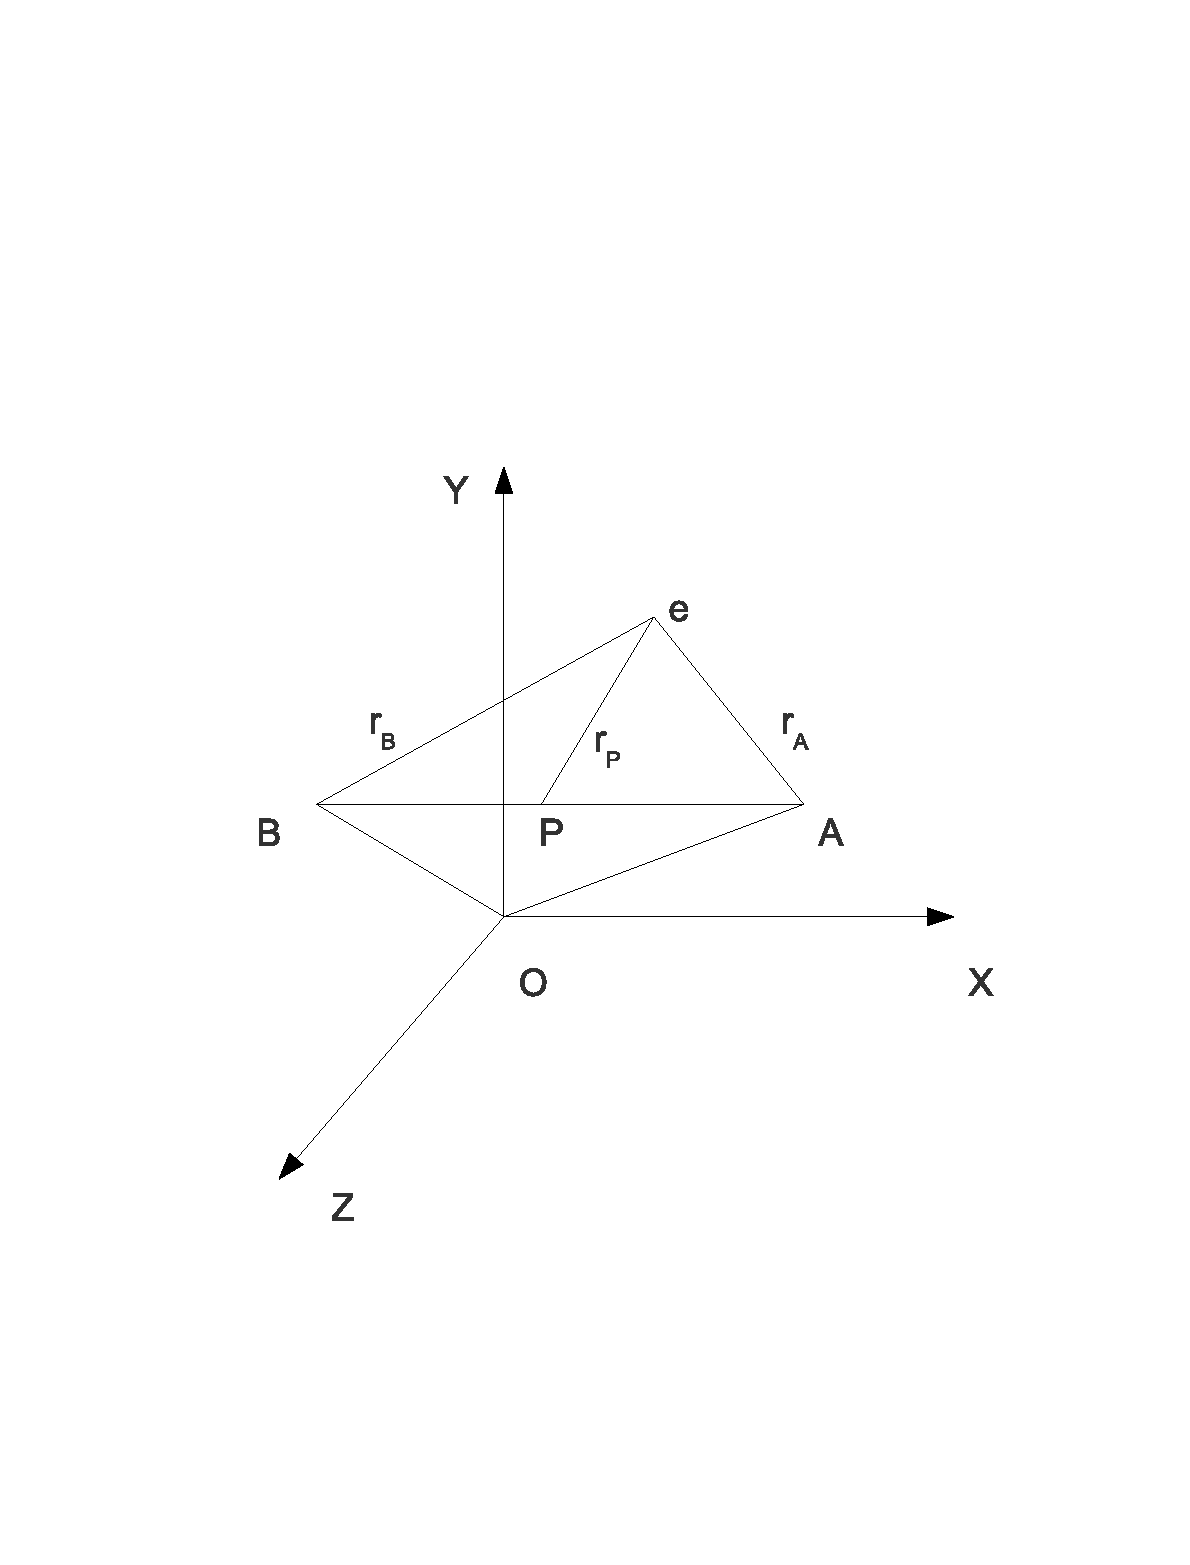
\includegraphics[scale=0.7]{gp.eps}
\caption{Gaussian primitive product theorem}
\label{fg:1}
\end{center}
\end{figure}

Now let's prove the simplest case, that both of the two primitive functions are S type of function; 
so the theorem can be stated as:
\begin{equation}
 \label{gaussian_product_rule_eq:1}
e^{-\alpha r_{A}^{2}}e^{-\beta r_{B}^{2}} = Ke^{-(\alpha+\beta) r_{P}^{2}}
\end{equation}
where $K$ is some constant.

Now let's prove it. By using the Cosine Rule, it's clear that:
\begin{align}
 \label{gaussian_product_rule_eq:2}
r_{A}^{2} &= r_{P}^{2} + \overline{PA}^{2} -2r_{P}\overline{PA}\cos\theta \nonumber \\
r_{B}^{2} &= r_{P}^{2} + \overline{PB}^{2} +2r_{P}\overline{PB}\cos\theta
\end{align}
Here $\theta$ is the angle formed by $\overline{AP}$ and $\overline{Pe}$.

Now let's get rid of the $\theta$. By multiplying $\overline{PB}$ to $r_{A}^{2}$, and 
multiplying $\overline{PA}$ to $r_{B}^{2}$ and add two equations in \ref{gaussian_product_rule_eq:2}
together; we can get:
\begin{equation}
 \label{gaussian_product_rule_eq:3}
\overline{PB}r_{A}^{2} + \overline{PA}r_{B}^{2} = \overline{AB}r_{P}^{2} + 
\overline{PA}\times\overline{PB}\times\overline{AB}
\end{equation}

However, in the exponent part of integral, besides the $r_{A}^{2}$ we have another factor 
of $\alpha$. Hence we have to find a way to associate the $\overline{PB}$ etc. with 
$\alpha$ so that to make up the exponent in the left hand side of \ref{gaussian_product_rule_eq:3}. 
It's easy to see that:
\begin{align}
 \label{gaussian_product_rule_eq:4}
\overline{PA} &= \frac{\beta}{\alpha+\beta}\overline{AB} \nonumber \\
\overline{PB} &= \frac{\alpha}{\alpha+\beta}\overline{AB}
\end{align}
Hence we can have:
\begin{equation}
\label{gaussian_product_rule_eq:5}
 \begin{split}
\frac{\alpha}{\alpha+\beta}\overline{AB}r_{A}^{2} +  
\frac{\beta}{\alpha+\beta}\overline{AB}r_{B}^{2} &= \overline{AB}r_{P}^{2} + 
\frac{\beta}{\alpha+\beta}\overline{AB}\frac{\alpha}{\alpha+\beta}\overline{AB}\times\overline{AB} 
 \end{split}
\end{equation}
Where we can get the result as:
\begin{equation}
\label{gaussian_product_rule_eq:6}
\alpha r_{A}^{2} + \beta r_{B}^{2} = (\alpha+\beta)r_{P}^{2} + \frac{\alpha\beta}{\alpha+\beta}
\overline{AB}^{2}
\end{equation}
Hence we have the final result as:
\begin{equation}
\label{gaussian_product_rule_eq:7}
e^{-\alpha r_{A}^{2} - \beta r_{B}^{2}} = 
e^{-(\alpha+\beta)r_{P}^{2}} e^{-\frac{\alpha\beta}{\alpha+\beta}
\overline{AB}^{2}}
\end{equation}

In the real calculation, it's necessary to know the P point location; that is to say, $P_{x}$ etc.
However, it's clear that the P's coordinate is determined by the $A$, $B$ and their exponents $\alpha$
and $\beta$:
\begin{equation}
 \label{gaussian_product_rule_eq:8}
\begin{split}
 \overline{PA} &= \frac{\beta}{\alpha+\beta}\overline{BA} \rightarrow \\
\overrightarrow{P} - \overrightarrow{A} &= \frac{\beta}{\alpha+\beta}
(\overrightarrow{B} - \overrightarrow{A}) \rightarrow  \\
\overrightarrow{P} &= \frac{\alpha}{\alpha+\beta}\overrightarrow{A} + 
\frac{\beta}{\alpha+\beta}\overrightarrow{B}
\end{split}
\end{equation}
So from here all of $P_{x}$, $P_{y}$ and $P_{z}$ can be got.

Now let's extend it to any arbitrary Gaussian primitives, that is to say; how we can express 
the following expression?
\begin{equation}
   x_{A}^{l_{1}}y_{A}^{m_{1}}z_{A}^{n_{1}}e^{-\alpha r_{A}^{2}}
   x_{B}^{l_{2}}y_{B}^{m_{2}}z_{B}^{n_{2}}e^{-\beta  r_{B}^{2}}   =  ?
\label{gaussian_product_rule_eq:9}
\end{equation}
for the $X_{A}$, since we have:
\begin{equation}
\begin{split}
 x_{A} &= e_{x} - A_{x} \\
       &= e_{x} - P_{x} + P_{x} - A_{x} \\
       &= x_{P} + \overline{PA}_{x} 
\end{split}
 \label{gaussian_product_rule_eq:10}
\end{equation}
Hence for the $x_{A}$ it totally converts into the expression related to $x_{P}$.

Similarly, for the $y_{A}$, $z_{A}$ etc. it's convenient to get their expressions too. So we can
finally convert the \ref{gaussian_product_rule_eq:9} into:
\begin{align}
&  x_{A}^{l_{1}}y_{A}^{m_{1}}z_{A}^{n_{1}}e^{-\alpha r_{A}^{2}}
   x_{B}^{l_{2}}y_{B}^{m_{2}}z_{B}^{n_{2}}e^{-\beta  r_{B}^{2}} \nonumber \\
=& (x_{P} + \overline{PA}_{x})^{l_{1}}(y_{P} + \overline{PA}_{y})^{m_{1}}
   (z_{P} + \overline{PA}_{z})^{n_{1}}e^{-\alpha r_{A}^{2}} \times \nonumber \\
&  (x_{P} + \overline{PB}_{x})^{l_{2}}(y_{P} + \overline{PB}_{y})^{m_{2}}
   (z_{P} + \overline{PB}_{z})^{n_{2}}e^{-\beta  r_{B}^{2}} \nonumber \\
=& (x_{P} + \overline{PA}_{x})^{l_{1}}(y_{P} + \overline{PA}_{y})^{m_{1}}
   (z_{P} + \overline{PA}_{z})^{n_{1}} \times \nonumber \\
&  (x_{P} + \overline{PB}_{x})^{l_{2}}(y_{P} + \overline{PB}_{y})^{m_{2}}
   (z_{P} + \overline{PB}_{z})^{n_{2}} \times \nonumber \\
&  e^{-(\alpha+\beta)r_{P}^{2}} e^{-\frac{\alpha\beta}{\alpha+\beta}
\overline{AB}^{2}}
  \label{gaussian_product_rule_eq:11}
\end{align}

In the practical calculation, usually it's required to separate the $x_{P}$ etc. from the 
$(x_{P} +\overline{PA}_{x})^{l_{1}}$. So according to binomial theorem we may have:
\begin{equation}
 (x_{P} +\overline{PA}_{x})^{l_{1}} = \sum_{i=0}^{l_{1}} x_{P}^{i}\overline{PA}_{x}^{l_{1}-i}
\binom{l_{1}}{i}
 \label{gaussian_product_rule_eq:12}
\end{equation}

Hence we could combine the two terms together:
\begin{equation}
\label{gaussian_product_rule_eq:13}
\begin{split}
(x_{P} +\overline{PA}_{x})^{l_{1}}(x_{P} + \overline{PB}_{x})^{l_{2}}
&=  \sum_{i=0}^{l_{1}} x_{P}^{i}\overline{PA}_{x}^{l_{1}-i}
\binom{l_{1}}{i}
    \sum_{j=0}^{l_{2}} x_{P}^{j}\overline{PB}_{x}^{l_{2}-j}
\binom{l_{2}}{j} \\
&= \sum_{k=0}^{l_{1}+l_{2}}x_{P}^{k}
\sum_{i=0,j=k-i}^{i=l_{1},j=l_{2}}\overline{PA}_{x}^{l_{1}-i}
\overline{PB}_{x}^{l_{2}-j}\binom{l_{1}}{i}\binom{l_{2}}{j}
\end{split}
\end{equation}

Now let's make some further analysis to the result shown in the \ref{gaussian_product_rule_eq:13}.
The term involves $i,j$ together actually is not convenient for computation purpose, hence we should
make it easier. Firstly we noticed that for the index $i$ we have such restrictions:
\begin{equation}
 \begin{cases}
  &0 \leq i \leq l_{1} \\
  &k-l_{2} \leq i \leq k
 \end{cases}
\end{equation}
$i\leq k$ is because that $i+j=k$ and $j\geq 0$. $i\geq k-l_{2}$ is because $l_{2} - k+i \geq 0$ in 
the \ref{gaussian_product_rule_eq:13}. Therefore the problem here is how can we sort out the 
real range of $i$?

Now we can guess that \ref{gaussian_product_rule_eq:13} perhaps can be rearranged into the form 
below\footnote{In practice we have tested the expression below for the $(x+a)^{3}(x+b)^{2}$, but
the proof can demonstrate that it's true for all of cases}:
\begin{multline}
\label{gaussian_product_rule_eq:14}
 (x_{P} +\overline{PA}_{x})^{l_{1}}(x_{P} + \overline{PB}_{x})^{l_{2}} = \\
\sum_{k=0}^{l_{1}+l_{2}}x_{P}^{k} 
\sum_{i=max(0,k-l_{2})}^{i=min(k,l_{1})}\overline{PA}_{x}^{l_{1}-i}
\overline{PB}_{x}^{l_{2}-k+i}\binom{l_{1}}{i}\binom{l_{2}}{k-i}
\end{multline}

Now let's literally prove it. Suggest we have the expression below:
\begin{align}
\label{gaussian_product_rule_eq:15}
 (x_{P} +\overline{PA}_{x})^{l_{1}}(x_{P} + \overline{PB}_{x})^{l_{2}} &= 
\sum_{i=0}^{l_{1}} x_{P}^{i}\overline{PA}_{x}^{l_{1}-i}
\binom{l_{1}}{i}
    \sum_{j=0}^{l_{2}} x_{P}^{j}\overline{PB}_{x}^{l_{2}-j}
\binom{l_{2}}{j} \nonumber \\
&=\sum_{k=0}^{l_{1}+l_{2}}x_{P}^{k} f_{k}(i,j,l_{1},l_{2},\overline{PA}_{x},\overline{PB}_{x})
\end{align} 
Where $i+j = k$, and $f_{k}$ expressed as:
\begin{equation}
\label{gaussian_product_rule_eq:16}
 f_{k}(i,j,l_{1},l_{2},\overline{PA}_{x},\overline{PB}_{x}) = 
\sum_{?}^{?}
\overline{PA}_{x}^{l_{1}-i}
\overline{PB}_{x}^{l_{2}-j}\binom{l_{1}}{i}\binom{l_{2}}{j}
\end{equation}

It's easy to know, that for each fixed $k$ value, $(i=0,j=k), (i=1,j=k-1), \cdots, 
(i=k,j=0)$ contribute to the $f_{k}$. However, since $i$ and $j$ are also limited by the 
$l_{1}$ and $l_{2}$, the $i$ and $j$ may not be able to take all of the pairs shown before.  
Now the problem is, if we very $i$ freely, and take $j=k-i$; then what's the range of $i$
in variation? 

Firstly let's consider the starting point of $i$. Obviously $i$ could start from $0$, however;
if $i=0$, then for a fixed $k$ then $j$ is $j=k-0=k$. But $j$ has a upper limit which is 
$j\leq l_{2}$, and it could have the situation that $l_{2} \leq k$. Hence in this situation, 
where $l_{2} \leq k$, then the minimum value of $i$ could not be $0$, but the value of $k-l_{2}$
since the maximum value of $j$ is $l_{2}$. The analysis here indicates that for the starting 
point of $i$, we should use ``max'' function for the $(0, k-l_{2})$.

Second let's go to see the end point of $i$. The $i$ could be $l_{1}$ from its definition,
however; as $i=l_{1}$ then $j=k-i=k-l_{1}$ that we may have the situation of $k-l_{1}\leq 0$.
Since $j$ must be larger or equal to zero so that the maximum number of $i$ could be $k$ 
(if $l_{1}\geq k$) or could be $l_{i}$ (if $l_{1}\leq k$). In this case, we have a minimum 
function of ``min'' between $(k,l_{1})$.

Finally, we note that the range analysis does not change the mathematical expression in the 
\ref{gaussian_product_rule_eq:16}. Hence the proof is ended. 

Now in the \ref{gaussian_product_rule_eq:16}, we are going to drop the index of $i$, $j$ from
the $f_{k}$ variable list since $i$ is summed over in the expression, and $j=k-i$ so that solely
determined by $i$ and $k$; hence we have:
\begin{equation}
\label{gaussian_product_rule_eq:17}
 (x_{P} +\overline{PA}_{x})^{l_{1}}(x_{P} + \overline{PB}_{x})^{l_{2}} = 
\sum_{k=0}^{l_{1}+l_{2}}x_{P}^{k}f_{k}(l_{1},l_{2},\overline{PA}_{x},\overline{PB}_{x}) 
\end{equation}
and $f_{k}$ is:
\begin{equation}
 \label{gaussian_product_rule_eq:18_0}
f_{k}(l_{1},l_{2},\overline{PA}_{x},\overline{PB}_{x}) = 
\sum_{i=max(0,k-l_{2})}^{i=min(k,l_{1})}\overline{PA}_{x}^{l_{1}-i}
\overline{PB}_{x}^{l_{2}-k+i}\binom{l_{1}}{i}\binom{l_{2}}{k-i}
\end{equation}

The expression in the \ref{gaussian_product_rule_eq:18} actually only applies for the situation 
that both $l_{1}$ and $l_{2}$ larger than zero. For the cases that $l_{1}$ or $l_{2}$ equal to zero,
we can directly use the binomial theorem to get the result. Hence the final result for the 
$f_{k}$ could be expressed as:
\begin{align}
\label{gaussian_product_rule_eq:18}
 &f_{k}(l_{1},l_{2},\overline{PA}_{x},\overline{PB}_{x}) \nonumber \\
&=
\begin{cases}
\sum_{i=max(0,k-l_{2})}^{i=min(k,l_{1})}\overline{PA}_{x}^{l_{1}-i}
\overline{PB}_{x}^{l_{2}-k+i}\binom{l_{1}}{i}\binom{l_{2}}{k-i}
    & l_{1} > 0, l_{2} > 0 \\
\overline{PA}_{x}^{l_{1}-k}\binom{l_{1}}{k}  
&  l_{1} > 0, l_{2} = 0 \\
\overline{PB}_{x}^{l_{2}-k}\binom{l_{2}}{k}  
&  l_{1} = 0, l_{2} > 0 \\
1                                           
&  l_{1} = 0, l_{2} = 0
\end{cases}
\end{align} 

Based on this result, for two arbitrary Gaussian primitives product on different center; 
we have the result as:
\begin{align}
&  x_{A}^{l_{1}}y_{A}^{m_{1}}z_{A}^{n_{1}}e^{-\alpha r_{A}^{2}}
   x_{B}^{l_{2}}y_{B}^{m_{2}}z_{B}^{n_{2}}e^{-\beta  r_{B}^{2}} \nonumber \\
=& \sum_{i=0}^{l_{1}+l_{2}}x_{P}^{i}f_{i}(l_{1},l_{2},\overline{PA}_{x},\overline{PB}_{x})  
   \times \nonumber \\
 & \sum_{j=0}^{m_{1}+m_{2}}y_{P}^{j}f_{j}(m_{1},m_{2},\overline{PA}_{y},\overline{PB}_{y})  
   \times \nonumber \\
 & \sum_{k=0}^{n_{1}+n_{2}}z_{P}^{k}f_{k}(n_{1},n_{2},\overline{PA}_{z},\overline{PB}_{z})  
   \times \nonumber \\
 &  e^{-(\alpha+\beta)r_{P}^{2}} e^{-\frac{\alpha\beta}{\alpha+\beta}\overline{AB}^{2}}
   \Rightarrow \nonumber \\
 & =\sum_{i=0}^{l_{1}+l_{2}}\sum_{j=0}^{m_{1}+m_{2}}\sum_{k=0}^{n_{1}+n_{2}}
   x_{P}^{i}y_{P}^{j}z_{P}^{k}
   e^{-(\alpha+\beta)r_{P}^{2}} e^{-\frac{\alpha\beta}{\alpha+\beta}\overline{AB}^{2}}
   \times F_{ijk}
  \label{gaussian_product_rule_eq:19}
\end{align}
Where $F_{ijk}$ is:
\begin{multline}
  F_{ijk} = \\
            f_{i}(l_{1},l_{2},\overline{PA}_{x},\overline{PB}_{x})
            f_{j}(m_{1},m_{2},\overline{PA}_{y},\overline{PB}_{y})
            f_{k}(n_{1},n_{2},\overline{PA}_{z},\overline{PB}_{z}) 
 \label{gaussian_product_rule_eq:20}
\end{multline}

Finally we note that for the same center situation, things is much more easier:
\begin{align}
&  x_{A}^{l_{1}}y_{A}^{m_{1}}z_{A}^{n_{1}}e^{-\alpha r_{A}^{2}}
   x_{A}^{l_{2}}y_{A}^{m_{2}}z_{A}^{n_{2}}e^{-\beta  r_{A}^{2}} \nonumber \\
=& x_{A}^{l_{1}+l_{2}}y_{A}^{m_{1}+m_{2}}z_{A}^{n_{1}+n_{2}}e^{-(\alpha+\beta)r_{A}^{2}}
  \label{gaussian_product_rule_eq:21}
\end{align} 


%%%%%%%%%%%%%%%%%%%%%%%%%%%%%%%%%%%%%%%%%%%%%%%%%%%%%%%%%%%%%%%%%%%%%%%%%%%%%%%%%%%%%%%%%%%%%%%%
\section{Shell Pair Data}
%
%
%
%
The Gaussian Primitive Product Theorem plays an key role in quantum chemistry\cite{SFBoys1950}. This
theorem is the key to understand that why we introduce the Gaussian type functions into the quantum 
chemistry; after all, the Slater type of function is more like the real wave function for atom system.
However, the integral for STO is too expensive to evaluate so that  we can use the linear combination 
of Gaussian functions to imitate the Slater functions, then to simulate the wave functions for atom.
Such idea is the crucial point for building the basis sets which is generally used in quantum chemistry
package.

In quantum chemistry, the electron integral could be generally expressed as:
\begin{equation}
 \label{shell_pair_eq:1}
I = \sum_{i=1}^{K}\sum_{j=1}^{K}\sum_{k=1}^{K}\sum_{l=1}^{K}
\int \int \chi_{i}^{*}(r)\chi_{j}^{*}(r)f(r,r^{'})
\chi_{k}(r^{'})\chi_{l}(r^{'}) dr dr^{'}
\end{equation}
Here $\chi$ is the Gaussian primitive function with arbitrary angular momentum, and $f(r,r^{'})$ is the 
electron operator for one or two electrons. Generally through the Gaussian Primitive Product Theorem, 
we could firstly combine the $ \chi_{i}^{*}(r)\chi_{j}^{*}(r)$ together into a new Gaussian function, 
so as for the $\chi_{k}(r^{'})\chi_{l}(r^{'})$. Therefore, the integral has been simplified into some
new form which only has two Gaussian functions.

Formally, we could designate the $ \chi_{i}^{*}(r)\chi_{j}^{*}(r)$ as ``shell pair'', which is 
physically related to the electron density (when multiply with MO coefficients etc.):
\begin{align}
\label{shell_pair_eq:2}
 \chi_{i}^{*}(r)\chi_{j}^{*}(r) \Longrightarrow (ij| \nonumber \\
 \chi_{k}(r^{'})\chi_{l}(r^{'}) \Longrightarrow |kl)
\end{align}
Such concept is trivial physically, but could bring great benefit for designing the software. 
Therefore, any analytical electron integrals we discuss later will be realized based on the shell pair
data.
    

%%%%%%%%%%%%%%%%%%%%%%%%%%%%%%%%%%%%%%%%%%%%%%%%%%%%%%%%%%%%%%%%%%%%%%%%%%%%%%%%%%%%%%%%%%%%%%%%
\section{Hermite Polynomials in Shell Pair Data}
%
%
%
%
In section \label{Gaussian_Primitive_Product_Theorem}, we have derived the shell pair data as:
\begin{equation}
\label{basic_shell_pair_data_form}
 |\chi_{A}\chi_{B}) = 
\begin{cases}
 \sum_{i=0}^{l_{1}+l_{2}}\sum_{j=0}^{m_{1}+m_{2}}\sum_{k=0}^{n_{1}+n_{2}}
   x_{P}^{i}y_{P}^{j}z_{P}^{k}
   e^{-(\alpha+\beta)r_{P}^{2}} e^{-\frac{\alpha\beta}{\alpha+\beta}\overline{AB}^{2}}
   \times F_{ijk}  \\
 x_{A}^{l_{1}+l_{2}}y_{A}^{m_{1}+m_{2}}z_{A}^{n_{1}+n_{2}}e^{-(\alpha+\beta)r_{A}^{2}}
\end{cases}
\end{equation}
It turns out that the complexity behind the shell pair data is brought by the angular momentum part.
For some arbitrary angular momentum number, each combination will introduce three sums hence
for two electron integral at least six round of sums is needed. Therefore, it implies that the 
angular momentum is the potential bottle neck for the integral evaluation.

Is there any way to avoid direct calculation of angular momentum part? Physically, the angular 
momentum part for atom wave function is generated by the central field; which turns out to be 
in form of $Y^{m}_{l}(\theta,\phi)$, and this is a set of orthogonal functions(see 
\ref{Transformation_Cart_sphere} for more information). Therefore, it implies that we could also
express the angular momentum part into other set of orthogonal functions (here we may need some
transformation, which finally convert it back to the Cartesian form or spherical form of 
basis set functions). The new form of basis set functions may bring us extra benefit in calculating
the integrals.
 
McMurchie and Davidson showed that\cite{MD} it's possible to use the
Hermite polynomials to achieve such transformation. Typically, they defined the
new angular momentum part in the Gaussian primitive functions as:
\begin{equation}
 \label{Shell_pair_data_further_eq:1}
\Lambda_{n}(\alpha, x_{p}) = e^{\alpha x_{p}^{2}} \frac{\partial^{n}}{\partial
P_{X}^{n}}\left( e^{-\alpha x_{p}^{2}} \right) 
\end{equation}
Here $x_{p}$ is defined the same as in \ref{gaussian_product_rule_eq:10}, which
is $x_{p} = e_{x} - P_{x}$. Now with the transformation that
\begin{equation}
 \label{Shell_pair_data_further_eq:2}
\frac{\partial}{\partial P_{x}} =
\frac{\partial}{\partial \sqrt{\alpha}x_{p}}\frac{\partial \sqrt{\alpha}x_{p}
}{\partial P_{x}} = -\sqrt{\alpha} \frac{\partial}{\partial \sqrt{\alpha}x_{p}}
\end{equation}
we can have:
\begin{equation}
 \label{Shell_pair_data_further_eq:3}
\Lambda_{n}(\alpha, x_{p}) = e^{\alpha x_{p}^{2}} (-\sqrt{\alpha})^{n}
 \frac{\partial^{n}}{\partial (\sqrt{\alpha}x_{p})^{n}}\left( e^{-\alpha
x_{p}^{2}} \right) \Rightarrow \Lambda_{n}(\alpha, x_{p}) =
\sqrt{\alpha}^{n}H_{n}(\sqrt{\alpha}x_{p})
\end{equation}
Now the $\Lambda$ is directly associated with the Hermite polynomials.

Furthermore, it's shown that:
\begin{equation}
 \label{Shell_pair_data_further_eq:4}
(x_{P} +\overline{PA}_{x})^{l_{1}}(x_{P} + \overline{PB}_{x})^{l_{2}}
= \sum^{l_{1}+l_{2}}_{k=0}d^{l_{1},l_{2}}_{k}\Lambda_{k}(\alpha, x_{p})
\end{equation}
Now the key to the problem is that how can we derive the $d$ in the 
\ref{Shell_pair_data_further_eq:4}.

Through the recursive relation for Hermite polynomials in
\ref{hermite_definition_eq:6}:
\begin{equation}
\label{Shell_pair_data_further_eq:5}
 2(\alpha^{\frac{1}{2}}x_{p})H_{n}(\alpha^{\frac{1}{2}}x_{p}) =
2nH_{n-1}(\alpha^{\frac{1}{2}}x_{p}) + H_{n+1}(\alpha^{\frac{1}{2}}x_{p})
\end{equation}
Now multiplying with $\alpha^{\frac{n-1}{2}}$ we can get:
\begin{equation}
 \label{Shell_pair_data_further_eq:6}
2x_{p}\alpha^{\frac{n}{2}}H_{n}(\alpha^{\frac{1}{2}}x_{p}) =
2n\alpha^{\frac{n-1}{2}}H_{n-1}(\alpha^{\frac{1}{2}}x_{p}) +
\alpha^{\frac{n-1}{2}}H_{n+1}(\alpha^{\frac{1}{2}}x_{p})
\end{equation}
Then we have:
\begin{equation}
 \label{Shell_pair_data_further_eq:7}
2x_{p}\Lambda_{n}(\alpha,x_{p}) = 2n\Lambda_{n-1}(\alpha,x_{p}) +
\alpha^{-1}\Lambda_{n+1}(\alpha,x_{p})
\end{equation}

Now let's set $x_{p} = e_{x} - P_{x} = e_{x} - A_{x} + A_{x} - P_{x} = 
x_{A} - \overline{PA}_{x} $, then we have:
\begin{equation}
\label{Shell_pair_data_further_eq:8}
2x_{A}\Lambda_{n}(\alpha,x_{p}) = 2n\Lambda_{n-1}(\alpha,x_{p}) +
2\overline{PA}_{x}\Lambda_{n}(\alpha,x_{p}) +
\alpha^{-1}\Lambda_{n+1}(\alpha,x_{p}) 
\end{equation}

Now let's combine the \ref{Shell_pair_data_further_eq:8} with 
\ref{Shell_pair_data_further_eq:4}, we can have that:
\begin{equation}
 \label{Shell_pair_data_further_eq:9}
\begin{split}
 (x_{A})^{l_{1}}(x_{B})^{l_{2}}
&= \sum^{l_{1}+l_{2}}_{n=0}d^{l_{1},l_{2}}_{n}\Lambda_{n}(\alpha, x_{p}) \Rightarrow \\
(x_{A})^{l_{1}+1}(x_{B})^{l_{2}}  
&= \sum^{l_{1}+l_{2}}_{n=0}x_{A}d^{l_{1},l_{2}}_{n}\Lambda_{n}(\alpha, x_{p}) \\
&= \sum^{l_{1}+l_{2}}_{n=0}d^{l_{1},l_{2}}_{n}\left[ n\Lambda_{n-1}(\alpha,x_{p}) +
\overline{PA}_{x}\Lambda_{n}(\alpha,x_{p}) +
\frac{1}{2\alpha}\Lambda_{n+1}(\alpha,x_{p}) \right] \\
&= \sum^{l_{1}+l_{2}}_{n=0}\left(
(n+1)d^{l_{1},l_{2}}_{n+1}             + 
\overline{PA}_{x}d^{l_{1},l_{2}}_{n}   +
\frac{1}{2\alpha}d^{l_{1},l_{2}}_{n-1}
 \right)\Lambda_{n}(\alpha,x_{p}) 
\end{split}
\end{equation}

On the other hand, for the $(x_{A})^{l_{1}+1}(x_{B})^{l_{2}}$ we could expand it according to
the definition:
\begin{equation}
 \label{Shell_pair_data_further_eq:10}
(x_{A})^{l_{1}+1}(x_{B})^{l_{2}}  = 
\sum^{l_{1}+1+l_{2}}_{n=0}d^{l_{1}+1,l_{2}}_{n}\Lambda_{n}(\alpha, x_{p})
\end{equation}
Therefore, we have:
\begin{equation}
 \label{Shell_pair_data_further_eq:11}
\sum^{l_{1}+1+l_{2}}_{n=0}d^{l_{1}+1,l_{2}}_{n}\Lambda_{n}(\alpha, x_{p}) =
\sum^{l_{1}+l_{2}}_{n=0}\left(
(n+1)d^{l_{1},l_{2}}_{n+1}             + 
\overline{PA}_{x}d^{l_{1},l_{2}}_{n}   +
\frac{1}{2\alpha}d^{l_{1},l_{2}}_{n-1}
 \right)\Lambda_{n}(\alpha,x_{p})
\end{equation}
By applying the orthogonal relation for the Hermite polynomials, that means to multiply
$H_{n}(x)e^{x^{2}}$ to each side of above equation and integrate it, we could have the 
recursive relation for the $d$:
\begin{equation}
 \label{Shell_pair_data_further_eq:12}
d^{l_{1}+1,l_{2}}_{n} = (n+1)d^{l_{1},l_{2}}_{n+1}             + 
\overline{PA}_{x}d^{l_{1},l_{2}}_{n}   +
\frac{1}{2\alpha}d^{l_{1},l_{2}}_{n-1}
\end{equation}
We note that this only applies for the situation of $n\geq 1$. On the other hand, we note
that in the \ref{Shell_pair_data_further_eq:8} we could also expand the $x_{p}$ as:
\begin{equation}
 x_{p} = e_{x} - P_{x} = e_{x} - B_{x} + B_{x} - P_{x} = 
x_{B} - \overline{PB}_{x} 
\end{equation}
Therefore by same procedure we can have:
\begin{equation}
 \label{Shell_pair_data_further_eq:13}
d^{l_{1},l_{2}+1}_{n} = (n+1)d^{l_{1},l_{2}}_{n+1}             + 
\overline{PB}_{x}d^{l_{1},l_{2}}_{n}   +
\frac{1}{2\alpha}d^{l_{1},l_{2}}_{n-1}
\end{equation}

The importance for the \ref{Shell_pair_data_further_eq:12} and \ref{Shell_pair_data_further_eq:13},
is that it indicates the integral could be evaluated through some ``recursive'' method. By starting
from the S type integral, we could gradually increase the order of angular momentums so that to
get integrals fro an arbitrary order of angular momentum. 
 

%
% now OS is already added in;
% will add the MD algorithm as well as DRK too in the future
% fm will be done in the near future
% 
%
%
%%%%%%%%%%%%%%%%%%%%%%%%%%%%%%%%%%%%%%%%%%%%%%%%%%%%%%%%%%%%%%%%%%%%%%%%%%%%%%%%%%%%%%%%%%%%
\chapter{Algorithms for Integral Evaluation Over Gaussian Functions}
%
%
%
%
%

In this chapter, we will focus on the electron integrals; which generally has the form as:
\begin{equation}
 V_{ij} = \int \chi_{i}(r)\chi_{j}(r)f(r,r^{'})
\chi_{k}(r^{'})\chi_{l}(r^{'}) dr dr^{'}
\end{equation}
It is already shown in the shell pair data discussion\ref{shell_pair_eq:1}. Here $\chi$ is 
the Gaussian primitive function with arbitrary angular momentum, and $f(r,r^{'})$ is the 
electron operator for one or two electrons. In this chapter, we will discuss the integrals
and its derivatives.

%%%%%%%%%%%%%%%%%%%%%%%%%%%%%%%%%%%%%%%%%%%%%%%%%%%%%%%%%%%%%%%%%%%%%%%%%%%%%%%%%%%%%%%%%%%%
\section{History for Algorithms of Integral Evaluation}
%
%
%
%
According to the general review given by Peter Gill\cite{gill1994molecular}, the history for
the development of integral algorithm could be divided into three period of times. The first
one is its infant period, at this time only simple SCF calculation could be performed. The 
first algorithm for Gaussian functions was prompted by Boys\cite{SFBoys1950},
then his methodology was subsequently developed by
Shavitt\cite{1963_int_algorithm}, Clementi etc.
\cite{clementi1969study,clementi1972computation}.

In the second generation, the SCF algorithm was mean to be more general. The ``axis-switch''
method of Pople and Hehre(PH)\cite{PH} revolutionized the algorithms of integral in a sense 
that it enables the SCF calculations to be a standard tool for the chemists. However, this method
is constructed primarily for the S and P type of Gaussian functions. Such deficiency motivated
the development of Dupuis-Rys-King(DRK)\cite{DRK1976JCP, DRK1976JCOMP, DRK1983JCOMP} method 
and McMurchie-Davidson(MD)\cite{MD} method to give more general derivation for the integrals.

The third generation of integral algorithm started from the Obara-Saika method(OS)\cite{OS1986,
OS1988} method, it is derived from the idea to solve the derivatives of integral\cite{HB1982,HB1989}. 
Encouraged by its success, a number of new algorithms came out\cite{HGP,gill1989efficient,
gill1990efficient,PRISM,coldprism} which constitutes the fundamental
layer for modern quantum chemistry packages. 

In this chapter, we will mainly focus on the second and third generation of integral algorithms. 
Namely the MD and DRK methods, OS, HGP and PRISM methods.

%%%%%%%%%%%%%%%%%%%%%%%%%%%%%%%%%%%%%%%%%%%%%%%%%%%%%%%%%%%%%%%%%%%%%%%%%%%%%%%%
%% this is about the mathematically formulas for integral
% 
% firstly set up on May, 2011
%
% for direct calculation:
% checked the results for kinetic integral,  overlap integral, 
% and derivations for overlap.   June 2ed
% checked the derivation for nuclear attraction integral, fine.  June 13th
%
%

%%%%%%%%%%%%%%%%%%%%%%%%%%%%%%%%%%%%%%%%%%%%%%%%%%%%%%%%%%%%%%%%%%%%%%%%%%%%%%%%%%%%%%%%%%%%
\section{Direct Integrals Calculation}
%
%
%
%
In this section, we will show how to derive the one electron integrals in terms of the 
basic form of shell pair data shown in \ref{basic_shell_pair_data_form}. Generally, such
way of derivation is simple and the efficiency is low; therefore in the modern quantum 
chemistry package it's not used anymore. However, it's still listed here for archive reason.
Furthermore, from the derivation we could clearly see how to make integral from the basic
way.

%%%%%%%%%%%%%%%%%%%%%%%%%%%%%%%%%%%%%%%%%%%%%%%%%%%%%%%%%%%%%%%%%%%%%%%%%%%%%%%%%%%%%%%%%%%%
\subsection{Overlap Integrals}
%
%
%
%
Now let's step into overlap integral. Firstly let's consider the simple S type of integral 
without contraction:
\begin{equation}
 \label{overlap_direct_int_eq:1}
\begin{split}
S_{\mu\nu}  &= \int \phi_{\mu}^{*}\phi_{\nu} dr \\
&= \int e^{-\alpha r_{A}^{2} - \beta r_{B}^{2}} dr \\
&= e^{-\frac{\alpha\beta}{\alpha+\beta}\overline{AB}^{2}}\int e^{-(\alpha+\beta)r_{P}^{2}} dr \\
&= e^{-\frac{\alpha\beta}{\alpha+\beta}\overline{AB}^{2}} \int e^{-(\alpha+\beta)x_{P}^{2}} dx
\int e^{-(\alpha+\beta)y_{P}^{2}} dy \int e^{-(\alpha+\beta)z_{P}^{2}} dz \\
&= e^{-\frac{\alpha\beta}{\alpha+\beta}\overline{AB}^{2}}\left( \frac{\pi}{\alpha+\beta}\right)
^{\frac{3}{2}}   
\end{split}
\end{equation}

The more common form of overlap integral between two arbitrary Gaussian primitives without 
contraction, will be given according to the \ref{gaussian_product_rule_eq:19} and 
\ref{gaussian_product_rule_eq:20}:
\begin{equation}
 \label{overlap_direct_int_eq:2}
\begin{split}
S_{\mu\nu}  &= \int \phi_{\mu}^{*}\phi_{\nu} dr \\
&= \int x_{A}^{l_{1}}y_{A}^{m_{1}}z_{A}^{n_{1}}
        x_{B}^{l_{2}}y_{B}^{m_{2}}z_{B}^{n_{2}}
        e^{-\alpha r_{A}^{2} - \beta r_{B}^{2}} dr \\
&= \int \sum_{i=0}^{l_{1}+l_{2}}\sum_{j=0}^{m_{1}+m_{2}}\sum_{k=0}^{n_{1}+n_{2}}
   x_{P}^{i}y_{P}^{j}z_{P}^{k}
   e^{-(\alpha+\beta)r_{P}^{2}} e^{-\frac{\alpha\beta}{\alpha+\beta}\overline{AB}^{2}}
   F_{ijk} dr \\
&= e^{-\frac{\alpha\beta}{\alpha+\beta}\overline{AB}^{2}}
   \sum_{i=0}^{l_{1}+l_{2}}\sum_{j=0}^{m_{1}+m_{2}}\sum_{k=0}^{n_{1}+n_{2}}F_{ijk}
   \int x_{P}^{i}y_{P}^{j}z_{P}^{k} e^{-(\alpha+\beta)r_{P}^{2}} dr \\
&= e^{-\frac{\alpha\beta}{\alpha+\beta}\overline{AB}^{2}}
   \sum_{i=0}^{l_{1}+l_{2}}\sum_{j=0}^{m_{1}+m_{2}}\sum_{k=0}^{n_{1}+n_{2}}F_{ijk}
   \int x_{P}^{i}e^{-(\alpha+\beta)x_{P}^{2}} dx \\
&\times
   \int y_{P}^{j}e^{-(\alpha+\beta)y_{P}^{2}} dy \int z_{P}^{k}e^{-(\alpha+\beta)z_{P}^{2}} dz  
\end{split}
\end{equation}

Now the integral has been retreated into simpler form. Now let's consider the integral form
of:
\begin{equation}
 \label{overlap_direct_int_eq:3}
 \int x^{i}e^{-\gamma x^{2}} dx
\end{equation}

This is the general form of integrals appearing in the \ref{overlap_direct_int_eq:2}. 
Firstly, we can
see that this integral only exists when $i$ is even number; that is to say:
\begin{equation}
\label{overlap_direct_int_eq:even}
 \int x^{i}e^{-\gamma x^{2}} dx = 0 \quad i = 2k+1
\end{equation}
This is because the function of $x^{i}e^{-\gamma x^{2}}$ is odd function when $i = 2k+1$. Hence 
here we have to make additional treatment, that to replace all of $i$, $j$ and $k$ in 
\ref{overlap_direct_int_eq:2} into $i^{'}$, $j^{'}$ and $k^{'}$:
\begin{equation}
 \begin{split}
  i &= 2*i^{'} \\ 
  j &= 2*j^{'} \\
  k &= 2*k^{'} 
 \end{split}
 \label{overlap_direct_int_eq:4}
\end{equation}

So the result in the \ref{overlap_direct_int_eq:2} can be rewritten as:
\begin{equation}
 \label{overlap_direct_int_eq:5}
\begin{split}
S_{\mu\nu}  &= \int \phi_{\mu}^{*}\phi_{\nu} dr \\
&= e^{-\frac{\alpha\beta}{\alpha+\beta}\overline{AB}^{2}}
   \sum_{i^{'}=0}^{\left[ \frac{l_{1}+l_{2}}{2}\right] }
   \sum_{j^{'}=0}^{\left[ \frac{m_{1}+m_{2}}{2}\right] }
   \sum_{k^{'}=0}^{\left[ \frac{n_{1}+n_{2}}{2}\right] }
   F_{2i^{'},2j^{'},2k^{'}}
   \int x_{P}^{2i^{'}}e^{-(\alpha+\beta)x_{P}^{2}} dx \\
&\times
   \int y_{P}^{2j^{'}}e^{-(\alpha+\beta)y_{P}^{2}} dy 
   \int z_{P}^{2k^{'}}e^{-(\alpha+\beta)z_{P}^{2}} dz  
\end{split}
\end{equation}

This integral, actually can be decomposed into three pieces:
\begin{equation}
 \label{overlap_direct_int_eq:6}
S_{\mu\nu} = e^{-\frac{\alpha\beta}{\alpha+\beta}\overline{AB}^{2}}
S_{\mu\nu}^{x}S_{\mu\nu}^{y}S_{\mu\nu}^{z}
\end{equation}

All of the three pieces are sharing the same structure:
\begin{align}
 \label{overlap_direct_int_eq:7}
S_{\mu\nu}^{x} &= \sum_{i^{'}=0}^{\left[ \frac{l_{1}+l_{2}}{2}\right] }
                  f_{2i^{'}}(l_{1},l_{2},\overline{PA}_{x},\overline{PB}_{x})
                  \int x_{P}^{2i^{'}}e^{-(\alpha+\beta)x_{P}^{2}} dx \nonumber \\
S_{\mu\nu}^{y} &= \sum_{j^{'}=0}^{\left[ \frac{m_{1}+m_{2}}{2}\right] }
                  f_{2j^{'}}(m_{1},m_{2},\overline{PA}_{y},\overline{PB}_{y})
                  \int y_{P}^{2j^{'}}e^{-(\alpha+\beta)y_{P}^{2}} dy \nonumber \\
S_{\mu\nu}^{z} &= \sum_{k^{'}=0}^{\left[ \frac{n_{1}+n_{2}}{2}\right] }
                  f_{2k^{'}}(n_{1},n_{2},\overline{PA}_{z},\overline{PB}_{z})
                  \int z_{P}^{2k^{'}}e^{-(\alpha+\beta)z_{P}^{2}} dz
\end{align}
According to the \ref{int_sec2_eq:8}, where the integral can be expressed as:
\begin{equation}
\int x^{2k}e^{-\alpha x^{2}} dx = 
\frac{(2k-1)!!\sqrt{\pi}}{(2\alpha)^{k}\sqrt{\alpha}}
\end{equation}
we can have that:
\begin{align}
 \label{overlap_direct_int_eq:8}
S_{\mu\nu}^{x} &= \sum_{i^{'}=0}^{\left[ \frac{l_{1}+l_{2}}{2}\right] }
                  f_{2i^{'}}(l_{1},l_{2},\overline{PA}_{x},\overline{PB}_{x})
                  \frac{(2i^{'}-1)!!\sqrt{\pi}}{(2(\alpha+\beta))^{i^{'}}\sqrt{\alpha+\beta}}
                  \nonumber \\
S_{\mu\nu}^{y} &= \sum_{j^{'}=0}^{\left[ \frac{m_{1}+m_{2}}{2}\right] }
                  f_{2j^{'}}(m_{1},m_{2},\overline{PA}_{y},\overline{PB}_{y})
                  \frac{(2j^{'}-1)!!\sqrt{\pi}}{(2(\alpha+\beta))^{j^{'}}\sqrt{\alpha+\beta}}
                  \nonumber \\
S_{\mu\nu}^{z} &= \sum_{k^{'}=0}^{\left[ \frac{n_{1}+n_{2}}{2}\right] }
                  f_{2k^{'}}(n_{1},n_{2},\overline{PA}_{z},\overline{PB}_{z})
                  \frac{(2k^{'}-1)!!\sqrt{\pi}}{(2(\alpha+\beta))^{k^{'}}\sqrt{\alpha+\beta}}
\end{align}
Now this is the result for the overlap integral between two arbitrary Gaussian primitives with
different centers.

For the overlap integral on the same center, according to the result in 
\ref{gaussian_product_rule_eq:21}, we will have that ($A=B$):
\begin{equation}
 \begin{split}
&\int x_{A}^{l_{1}}y_{A}^{m_{1}}z_{A}^{n_{1}}
        x_{B}^{l_{2}}y_{B}^{m_{2}}z_{B}^{n_{2}}
        e^{-\alpha r_{A}^{2} - \beta r_{B}^{2}} dr \\
&= \int x_{A}^{l_{1}+l_{2}}y_{A}^{m_{1}+m_{2}}z_{A}^{n_{1}+n_{2}}e^{-(\alpha+\beta)r_{A}^{2}} dr\\
&= 
\int x_{A}^{l_{1}+l_{2}}e^{-(\alpha+\beta)x_{A}^{2}} dx
\int y_{A}^{m_{1}+m_{2}}e^{-(\alpha+\beta)y_{A}^{2}} dy
\int z_{A}^{n_{1}+n_{2}}e^{-(\alpha+\beta)z_{A}^{2}} dz
 \end{split}
\label{overlap_direct_int_eq:9}
\end{equation}
According to the result in \ref{overlap_direct_int_eq:even}, the result will 
be quite interesting that
this integral is not zero only if $l_{1}+l_{2} = 2i$, $m_{1}+m_{2} = 2j$, $n_{1}+n_{2} = 2k$. 
Hence it's easy to see that integrals between S and P shell etc. are all zero. However, it does 
not mean that different shell types in the same center are orthogonal. For example, the integral
between PX and FXY2 are not zero.

For the integral, according to the result in \ref{int_sec2_eq:8}; the final result 
between same center could be expressed as:
\begin{equation}
 \label{overlap_direct_int_eq:10}
\begin{split}
 & 
\int x_{A}^{l_{1}+l_{2}}e^{-(\alpha+\beta)x_{A}^{2}} dx
\int y_{A}^{m_{1}+m_{2}}e^{-(\alpha+\beta)y_{A}^{2}} dy
\int z_{A}^{n_{1}+n_{2}}e^{-(\alpha+\beta)z_{A}^{2}} dz \\
&= \left( \frac{\pi}{\alpha+\beta}\right)^{\frac{3}{2}} 
\frac{(l_{1}+l_{2}-1)!!(m_{1}+m_{2}-1)!!(n_{1}+n_{2}-1)!!}
{(2(\alpha+\beta))^{\frac{l_{1}+l_{2}+m_{1}+m_{2}+n_{1}+n_{2}}{2}}}
\end{split}
\end{equation}
 
Finally, we step into the overlap integral for an arbitrary basis function of $\phi$, which is 
a set of contracted Gaussian primitives. Firstly we can record the result in 
\ref{overlap_direct_int_eq:6}
as $\langle\chi_{\mu}|\chi_{\nu}\rangle$ (but usually we express it as 
$\langle\chi_{i}|\chi_{j}\rangle$, since the $\mu$, $\nu$ label are related to the indices of 
basis set functions). The basis set function can be expressed as:
\begin{equation}
\begin{split}
\label{overlap_direct_int_eq:11}
 \phi_{\mu} &= \sum_{i}d_{\mu i}\chi_{i} \\
 \phi_{\nu} &= \sum_{j}d_{\mu j}\chi_{j} 
\end{split}
\end{equation}

Then based on the results in \ref{overlap_direct_int_eq:6}, \ref{overlap_direct_int_eq:7} 
and \ref{overlap_direct_int_eq:8}
we have:
\begin{equation}
 \label{overlap_direct_int_eq:12}
 S_{\mu\nu} = \sum_{i}\sum_{j}d_{\mu i}d_{\mu j}\langle\chi_{i}|\chi_{j}\rangle
\end{equation}
This is the final result for overlap integral.

%%%%%%%%%%%%%%%%%%%%%%%%%%%%%%%%%%%%%%%%%%%%%%%%%%%%%%%%%%%%%%%%%%%%%%%%%%%
\subsection{Derivatives for Overlap Integral} 

There's more advantages if we use Gaussian primitive function rather than the Slater type of function
in getting the derivatives of the integral. For a common Gaussian primitive, let's derive its 
derivatives we can see that:
\begin{equation}
 \label{derivative_overlap_direct_int_eq:1}
\frac{\partial \chi_{i}}{\partial R_{x}} = \frac{\partial (x^{l}y^{m}z^{n}e^{-\alpha r^{2}})}
{\partial R_{x}} =  -lx^{l-1}y^{m}z^{n}e^{-\alpha r^{2}} + 2\alpha x^{l+1}y^{m}z^{n}e^{-\alpha r^{2}}
\end{equation}
Here the $x$ is expressed as:
\begin{equation}
 x = x_{e} - R_{x} 
\end{equation}
Which is the $x$ difference between the electron position and the nuclear position. 

The expression is exactly equal to the form below:
\begin{equation}
 \label{derivative_overlap_direct_int_eq:2}
\frac{\partial \chi^{lmn}_{i}}{\partial R_{x}} = -l\chi_{i}^{l-1mn} + 2\alpha\chi_{i}^{l+1mn}
\end{equation}
This result shows that the derivatives for the Gaussian primitive can be expressed as the linear 
sum of two Gaussian primitives, one is with higher angular momentum and the other with lower
angular momentum; it indicates that the derivatives for the integral of Gaussian primitives 
can be simply expressed as some summation between the integrals.

The overlap integral between two Gaussian primitives, can be expressed as:
\begin{equation}
 \label{derivative_overlap_direct_int_eq:3}
\frac{\partial\langle\chi_{i}|\chi_{j}\rangle}{\partial R_{x}} = 
\begin{cases}
 0  \\
\left\langle \frac{\partial \chi_{i} }{\partial R_{x}}|\chi_{j}\right\rangle \quad \text{or}
\quad \left\langle \chi_{i}|\frac{\partial \chi_{j} }{\partial R_{x}}\right\rangle \\
\left\langle \frac{\partial \chi_{i} }{\partial R_{x}}|\chi_{j}\right\rangle +
\left\langle \chi_{i}|\frac{\partial \chi_{j} }{\partial R_{x}}\right\rangle
\end{cases}
\end{equation}
If both $\chi_{i}$ and $\chi_{j}$ do not center on the given atom ($R_{x}$), then the derivatives
is zero; if either $\chi_{i}$ or $\chi_{j}$ center on the given atom, the derivatives will be like
the second equation; finally if both $\chi_{i}$ and $\chi_{j}$ center on the given atom, the 
derivatives will be expressed as in the third equation. Now let's go to see how to express the 
second equation in terms of the \ref{derivative_overlap_direct_int_eq:2}:
\begin{equation}
 \begin{split}
  \left\langle \frac{\partial \chi_{i} }{\partial R_{x}}|\chi_{j}\right\rangle &=
-l_{i}\langle\chi_{i}^{l_{i}-1m_{i}n_{i}}|\chi_{j}\rangle
+2\alpha_{i}\langle\chi_{i}^{l_{i}+1m_{i}n_{i}}|\chi_{j}\rangle
 \end{split}
\label{derivative_overlap_direct_int_eq:4}
\end{equation}
while in literature, the integral shown above usually expressed in the other way:
\begin{equation}
 \label{derivative_overlap_direct_int_eq:5}
\left\langle \frac{\partial \chi_{i} }{\partial R_{x}}|\chi_{j}\right\rangle
= -l_{i}\langle -1|0\rangle_{x} + 2\alpha_{i}\langle +1 | 0\rangle_{x}
\end{equation}
Here ``0'' indicates its original form (like for the $\chi_{j}$, it's not changed so we label it
as 0), and ``$+1$'' or ``$-1$'' means the angular momentum is ascending or descending. Finally,
the subscript of ``x'' means the changing of angular momentum is on the x. This expression is 
simpler than the \ref{derivative_overlap_direct_int_eq:4}. 

%%%%%%%%%%%%%%%%%%%%%%%%%%%%%%%%%%%%%%%%%%%%%%%%%%%%%%%%%%%%%%%%%%%%%%%%%%%%%
\subsection{Kinetic Energy Integral}
%
%
%
Kinetic energy integral is defined as:
\begin{equation}
 \label{kinetic_direct_int_eq:1}
\begin{split}
 T_{ij} &= \int \chi_{i}(-\frac{1}{2}\nabla^{2})\chi_{j} dr \\
&= -\frac{1}{2} \int 
x^{l_{i}}y^{m_{i}}z^{n_{i}}e^{-\alpha_{i} r_{i}^{2}}
\left( 
  \frac{\partial^{2}}{\partial x^{2}}
+ \frac{\partial^{2}}{\partial y^{2}}
+ \frac{\partial^{2}}{\partial z^{2}}\right)
x^{l_{j}}y^{m_{j}}z^{n_{j}}e^{-\alpha_{j} r_{j}^{2}}
\end{split}
\end{equation}
It's easy to see that the integral here can be restored to the overlap integrals. We can do it directly
by expanding each term inside \ref{kinetic_direct_int_eq:1}, however; as we know, the kinetic energy should
be symmetric (as physically it's Hermitian operator); hence usually we evaluate the kinetic energy 
in another way. Here below is a simple example:
\begin{equation}
 \begin{split}
 & -\frac{1}{2} \int 
x^{l_{i}}y^{m_{i}}z^{n_{i}}e^{-\alpha_{i} r_{i}^{2}} 
  \frac{\partial^{2}}{\partial x^{2}}
x^{l_{j}}y^{m_{j}}z^{n_{j}}e^{-\alpha_{j} r_{j}^{2}} dxdydz \\
&=
-\frac{1}{2}  \int \left\lbrace 
x^{l_{i}}y^{m_{i}}z^{n_{i}}e^{-\alpha_{i} r_{i}^{2}}\left. 
\frac{\partial (x^{l_{j}}y^{m_{j}}z^{n_{j}}e^{-\alpha_{j} r_{j}^{2}})}{\partial x}
\right\rbrace 
\right|^{+\infty}_{-\infty} dydz
\\
&+ \frac{1}{2}  \int 
\frac{\partial (x^{l_{i}}y^{m_{i}}z^{n_{i}}e^{-\alpha_{i} r_{i}^{2}})}{\partial x}
\frac{\partial (x^{l_{j}}y^{m_{j}}z^{n_{j}}e^{-\alpha_{j} r_{j}^{2}})}{\partial x} dxdydz \\
&= \frac{1}{2}  \int 
\frac{\partial (x^{l_{i}}y^{m_{i}}z^{n_{i}}e^{-\alpha_{i} r_{i}^{2}})}{\partial x}
\frac{\partial (x^{l_{j}}y^{m_{j}}z^{n_{j}}e^{-\alpha_{j} r_{j}^{2}})}{\partial x} dxdydz
 \end{split}
\label{kinetic_direct_int_eq:2}
\end{equation}
The \ref{kinetic_direct_int_eq:2} is done through integral by parts. Here we can see that the $T_{ij}$
becomes symmetric, and the $T_{ij}$ is always larger than zero between two Gaussian primitives.

Let's make the evaluation a bit of simpler. If we denote the integral in \ref{kinetic_direct_int_eq:2} 
as $I_{x}$, it's easy to see that :
\begin{equation}
 T_{ij} = I_{x} + I_{y} + I_{z}
\end{equation}
for $I_{x}$ we have that:
\begin{equation}
 \label{kinetic_direct_int_eq:3}
\begin{split}
 I_{x} &=\frac{1}{2}   \int 
          \left[ l_{i}x^{l_{i}-1} - 2\alpha_{i}x^{l_{i}+1}\right]
          y^{m_{i}}z^{n_{i}}e^{-\alpha_{i} r_{i}^{2}} \\
       &\times
          \left[ l_{j}x^{l_{j}-1} - 2\alpha_{j}x^{l_{j}+1}\right]
          y^{m_{j}}z^{n_{j}}e^{-\alpha_{j} r_{j}^{2}} dr \\
       &= \frac{1}{2}\Big(
          l_{i}l_{j}\langle -1|-1\rangle_{x} 
        - 2\alpha_{i}l_{j}\langle +1|-1\rangle_{x}    \\
       &- 2\alpha_{j}l_{i}\langle -1|+1\rangle_{x}
        + 4\alpha_{i}\alpha_{j}\langle +1|+1\rangle_{x} 
          \Big) 
\end{split}
\end{equation}

Similarly for the $I_{y}$ and $I_{z}$ we have:
\begin{equation}
\label{kinetic_direct_int_eq:4}
\begin{split}
I_{y} &=  \frac{1}{2}\Big(
          m_{i}m_{j}\langle -1|-1\rangle_{y} 
        - 2\alpha_{i}m_{j}\langle +1|-1\rangle_{y}   \\ 
       &- 2\alpha_{j}m_{i}\langle -1|+1\rangle_{y}
        + 4\alpha_{i}\alpha_{j}\langle +1|+1\rangle_{y} 
          \Big) \\
I_{z} &=  \frac{1}{2}\Big(
          n_{i}n_{j}\langle -1|-1\rangle_{z} 
        - 2\alpha_{i}n_{j}\langle +1|-1\rangle_{z}   \\ 
       &- 2\alpha_{j}n_{i}\langle -1|+1\rangle_{z}
        + 4\alpha_{i}\alpha_{j}\langle +1|+1\rangle_{z} 
          \Big) 
\end{split}
\end{equation}
Now the kinetic energy integral is done.

%%%%%%%%%%%%%%%%%%%%%%%%%%%%%%%%%%%%%%%%%%%%%%%%%%%%%%%%%%%%%%%%%%%%%%%%%%%%%%%%%%
\subsection{Nuclear Attraction Integral}
\label{direct_NAI_derivation}
%
%
%
The common nuclear attraction integral between two arbitrary Gaussian primitives can be expressed
as:
\begin{equation}
 \begin{split}
  V &= \int \chi_{i}(r)\frac{1}{r_{C}}\chi_{j}(r) dr \\
&= \int x^{l_{A}}_{A}y^{m_{A}}_{A}z^{n_{A}}_{A}e^{-\alpha r_{A}^{2}}
        \frac{1}{r_{C}}
        x^{l_{B}}_{B}y^{m_{B}}_{B}z^{n_{B}}_{B}e^{-\beta  r_{B}^{2}} dr
 \end{split}
\label{nuclear_attraction_direct_int_eq:1}
\end{equation}
$r_{A}, r_{B}$ and $r_{c}$ denotes the distance between electron position and the given
nuclear (A, B or C).

This difficulty to solve this integral is for the $1/r_{C}$. However, we can use standard
Laplace transformation to convert it into another form:
\begin{equation}
\label{nuclear_attraction_direct_int_eq:2}
 \frac{1}{r_{C}} = \frac{1}{\sqrt{\pi}}\int^{\infty}_{0} e^{-sr_{C}^{2}} s^{-\frac{1}{2}} ds
\end{equation}
So that we have:
\begin{equation}
 \begin{split}
V &= \frac{1}{\sqrt{\pi}}\int^{\infty}_{0} e^{-sr_{C}^{2}} s^{-\frac{1}{2}} ds 
          \int x^{l_{A}}_{A}y^{m_{A}}_{A}z^{n_{A}}_{A}e^{-\alpha r_{A}^{2}}
          x^{l_{B}}_{B}y^{m_{B}}_{B}z^{n_{B}}_{B}e^{-\beta  r_{B}^{2}} dr \\
       &= \frac{1}{\sqrt{\pi}}\int^{\infty}_{0}  s^{-\frac{1}{2}} ds  
          \int e^{-sr_{C}^{2}} 
          x^{l_{A}}_{A}y^{m_{A}}_{A}z^{n_{A}}_{A}e^{-\alpha r_{A}^{2}}
          x^{l_{B}}_{B}y^{m_{B}}_{B}z^{n_{B}}_{B}e^{-\beta  r_{B}^{2}} dr
 \end{split}
\label{nuclear_attraction_direct_int_eq:3}
\end{equation}
Basically, this is equivalent to three-center overlap integral. So now let's think about
how to derive it.

Let's begin from the shell pair. In the \ref{nuclear_attraction_direct_int_eq:3} we could combine the 
A and B center together. According to the results in the 
\ref{gaussian_product_rule_eq:19} and \ref{gaussian_product_rule_eq:20}, we can express 
the integral above as:
\begin{multline}
  V = e^{-\frac{\alpha\beta}{\alpha+\beta}\overline{AB}^{2}} 
\sum_{i=0}^{l_{A}+l_{B}}f_{i}(l_{A},l_{B},\overline{PA}_{x},\overline{PB}_{x})
\sum_{j=0}^{m_{A}+m_{B}}f_{j}(m_{A},m_{B},\overline{PA}_{y},\overline{PB}_{y}) \times \\
\sum_{k=0}^{n_{A}+n_{B}}f_{k}(n_{A},n_{B},\overline{PA}_{z},\overline{PB}_{z}) 
   \frac{1}{\sqrt{\pi}} 
   \int^{\infty}_{0} s^{-\frac{1}{2}} ds 
   \int x_{P}^{i}y_{P}^{j}z_{P}^{k} e^{-(\alpha+\beta)r_{P}^{2}}e^{-sr_{C}^{2}} dr
\label{nuclear_attraction_direct_int_eq:6}
\end{multline}
So the problem is left to solve the integral inside the \ref{nuclear_attraction_direct_int_eq:6}.

Before proceeding on solving the integrals, it's very interesting to note that the function of 
$x_{P}^{i}y_{P}^{j}z_{P}^{k} e^{-(\alpha+\beta)r_{P}^{2}}e^{-sr_{C}^{2}}$ will not be zero if 
$i$, $j$ and $k$ is even number. So this is different from the overlap integral situation. 
The reason is because of $r_{C}$. For example, 
$ x_{P}^{i} e^{-(\alpha+\beta)x_{P}^{2}}e^{-sx_{C}^{2}} $ is not 
even or odd function as $i$ is even or odd number, that's all because of the $x_{C}$ in the 
integral.

Firstly let's concentrate on the integral over $r$, which is:
\begin{equation}
  \int x_{P}^{i}y_{P}^{j}z_{P}^{k} e^{-(\alpha+\beta)r_{P}^{2}}e^{-sr_{C}^{2}} dr
\end{equation}
According to the Gaussian primitive product theorem, this term can be finally expressed 
into:
\begin{equation}
\begin{split}
&\int x_{P}^{i}y_{P}^{j}z_{P}^{k} e^{-(\alpha+\beta)r_{P}^{2}}e^{-sr_{C}^{2}} dr  \\
&=
e^{-\frac{(\alpha+\beta)s}{\alpha+\beta + s} \overline{PC}^{2}}\times
\int(x_{Q}+\overline{QP}_{x})^{i}(y_{Q}+\overline{QP}_{y})^{j}(z_{Q}+\overline{QP}_{z})^{k}
e^{-(\alpha+\beta + s)r_{Q}^{2}} dr \\ 
&=
e^{-\frac{(\alpha+\beta)s}{\alpha+\beta + s} \overline{PC}^{2}}\times
\sum_{i^{'}=0}^{i}\sum_{j^{'}=0}^{j}\sum_{k^{'}=0}^{k}
\binom{i}{i^{'}}\binom{j}{j^{'}}\binom{k}{k^{'}}
\overline{QP}_{x}^{i-i^{'}}\overline{QP}_{y}^{j-j^{'}}\overline{QP}_{z}^{k-k^{'}} \\
&\int x_{Q}^{i^{'}}y_{Q}^{j^{'}}z_{Q}^{k^{'}} e^{-(\alpha+\beta+s)r_{Q}^{2}} dr
\end{split}
 \label{nuclear_attraction_direct_int_eq:7}
\end{equation}
Here Q is determined by the P point and C point.

For the expression in \ref{nuclear_attraction_direct_int_eq:7}, we note that 
$\int x_{Q}^{i^{'}}y_{Q}^{j^{'}}z_{Q}^{k^{'}} e^{-(\alpha+\beta+s)r_{Q}^{2}} dr$ is even function; 
which requires that the $i^{'}$, $j^{'}$ and $k^{'}$ are all even numbers. Therefore the integral
in the \ref{nuclear_attraction_direct_int_eq:7} could be transformed into:
\begin{equation}
\begin{split}
&\int x_{P}^{i}y_{P}^{j}z_{P}^{k} e^{-(\alpha+\beta)r_{P}^{2}}e^{-sr_{C}^{2}} dr  \\
&=
e^{-\frac{(\alpha+\beta)s}{\alpha+\beta + s} \overline{PC}^{2}}\times
\sum_{i^{'}=0}^{\left[ \frac{i}{2}\right] }
\sum_{j^{'}=0}^{\left[ \frac{j}{2}\right]}
\sum_{k^{'}=0}^{\left[ \frac{k}{2}\right]}
\binom{i}{2i^{'}}\binom{j}{2j^{'}}\binom{k}{2k^{'}}
\overline{QP}_{x}^{i-2i^{'}}\overline{QP}_{y}^{j-2j^{'}}\overline{QP}_{z}^{k-2k^{'}} \\
&\int x_{Q}^{2i^{'}}y_{Q}^{2j^{'}}z_{Q}^{2k^{'}} e^{-(\alpha+\beta+s)r_{Q}^{2}} dr
\end{split}
 \label{nuclear_attraction_direct_int_eq:7_1}
\end{equation}

The $\overline{QP}$ is also connected with variable $s$, according to the 
\ref{gaussian_product_rule_eq:8}, it has the form that:
\begin{equation}
 \overrightarrow{QP} = \frac{s}{\alpha+\beta+s}\overrightarrow{CP}
\end{equation}
Therefore the \ref{nuclear_attraction_direct_int_eq:7_1} could be further transformed into:
\begin{equation}
\begin{split}
&\int x_{P}^{i}y_{P}^{j}z_{P}^{k} e^{-(\alpha+\beta)r_{P}^{2}}e^{-sr_{C}^{2}} dr  \\
&=
e^{-\frac{(\alpha+\beta)s}{\alpha+\beta + s} \overline{PC}^{2}}\times
\sum_{i^{'}=0}^{\left[ \frac{i}{2}\right] }
\sum_{j^{'}=0}^{\left[ \frac{j}{2}\right]}
\sum_{k^{'}=0}^{\left[ \frac{k}{2}\right]}
\left( \frac{s}{\alpha+\beta+s}\right)^{i+j+k-2(i^{'}+j^{'}+k^{'})} \\
&\binom{i}{2i^{'}}\binom{j}{2j^{'}}\binom{k}{2k^{'}}
\overline{CP}_{x}^{i-2i^{'}}\overline{CP}_{y}^{j-2j^{'}}\overline{CP}_{z}^{k-2k^{'}} \\
&\int x_{Q}^{2i^{'}}y_{Q}^{2j^{'}}z_{Q}^{2k^{'}} e^{-(\alpha+\beta+s)r_{Q}^{2}} dr
\end{split}
 \label{nuclear_attraction_direct_int_eq:7_2}
\end{equation}

The integration result for the \ref{nuclear_attraction_direct_int_eq:7_2} can be expressed as according 
to \ref{int_sec2_eq:8}:
\begin{equation}
\begin{split}
 &\int x_{P}^{i}y_{P}^{j}z_{P}^{k} e^{-(\alpha+\beta)r_{P}^{2}}e^{-sr_{C}^{2}} dr  \\
&=
e^{-\frac{(\alpha+\beta)s}{\alpha+\beta + s} \overline{PC}^{2}}\times
\sum_{i^{'}=0}^{\left[ \frac{i}{2}\right]}
\sum_{j^{'}=0}^{\left[ \frac{j}{2}\right]}
\sum_{k^{'}=0}^{\left[ \frac{k}{2}\right]}
\left( \frac{s}{\alpha+\beta+s}\right)^{i+j+k-2(i^{'}+j^{'}+k^{'})} \\
&\binom{i}{2i^{'}}\binom{j}{2j^{'}}\binom{k}{2k^{'}}
\overline{CP}_{x}^{i-2i^{'}}\overline{CP}_{y}^{j-2j^{'}}\overline{CP}_{z}^{k-2k^{'}} \\
&\left( \frac{\pi}{\alpha+\beta+s}\right)^{\frac{3}{2}}\times
\frac{(2i^{'}-1)!!(2j^{'}-1)!!(2k^{'}-1)!!}
{(2(\alpha+\beta+s))^{i^{'}+j^{'}+k^{'}}} 
\end{split}
 \label{nuclear_attraction_direct_int_eq:8}
\end{equation}

Now let's consider the outer integral which is over $s$:
\begin{equation}
\begin{split}
&\frac{1}{\sqrt{\pi}} 
 \int^{\infty}_{0} s^{-\frac{1}{2}} ds 
 \int x_{P}^{i}y_{P}^{j}z_{P}^{k} e^{-(\alpha+\beta)r_{P}^{2}}e^{-sr_{C}^{2}} dr \\
&= 
\frac{1}{\sqrt{\pi}}
\sum_{i^{'}=0}^{\left[ \frac{i}{2}\right]}
\sum_{j^{'}=0}^{\left[ \frac{j}{2}\right]}
\sum_{k^{'}=0}^{\left[ \frac{k}{2}\right]} 
\pi^{\frac{3}{2}}\binom{i}{2i^{'}}\binom{j}{2j^{'}}\binom{k}{2k^{'}}
\overline{CP}_{x}^{i-2i^{'}}\overline{CP}_{y}^{j-2j^{'}}\overline{CP}_{z}^{k-2k^{'}} \\
&\frac{(2i^{'}-1)!!(2j^{'}-1)!!(2k^{'}-1)!!}{2^{i^{'}+j^{'}+k^{'}}} 
\int^{\infty}_{0} ds s^{-\frac{1}{2}}
e^{-\frac{(\alpha+\beta)s}{\alpha+\beta + s} \overline{PC}^{2}} \\
&(\alpha+\beta+s)^{-\left( i^{'}+j^{'}+k^{'}+\frac{3}{2}\right) } 
\left( \frac{s}{\alpha+\beta+s}\right)^{i+j+k-2(i^{'}+j^{'}+k^{'})}
\end{split}
 \label{nuclear_attraction_direct_int_eq:11}
\end{equation}

Let's suggest to make variable transformation, that:
\begin{equation}
 \label{nuclear_attraction_direct_int_eq:12}
\frac{s}{\alpha+\beta + s} = t^{2}
\end{equation}
So that as $s$ goes from $0$ to $\infty$, then $t$ could be from $0$ to $1$.

If we differentiate it, we could get:
\begin{equation}
 \label{nuclear_attraction_direct_int_eq:13}
\frac{\alpha+\beta}{(\alpha+\beta + s)^{2}} ds = 2tdt \Rightarrow ds = 
2s^{\frac{1}{2}}\frac{(\alpha+\beta + s)^{\frac{3}{2}}}{\alpha+\beta} dt
\end{equation}

Now let's bring the \ref{nuclear_attraction_direct_int_eq:13} into the 
\ref{nuclear_attraction_direct_int_eq:11}. Furthermore, we write:
\begin{equation}
 \begin{split}
  i+j+k             &= L \\
  i^{'}+j^{'}+k^{'} &= L^{'}
 \end{split}
\end{equation}

Therefore we have:
\begin{equation}
 \label{nuclear_attraction_direct_int_eq:14}
\begin{split}
&\frac{1}{\sqrt{\pi}} 
 \int^{\infty}_{0} s^{-\frac{1}{2}} ds 
 \int x_{P}^{i}y_{P}^{j}z_{P}^{k} e^{-(\alpha+\beta)r_{P}^{2}}e^{-sr_{C}^{2}} dr \\
&= 
\frac{2\pi}{\alpha+\beta}
\sum_{i^{'}=0}^{\left[ \frac{i}{2}\right]}
\sum_{j^{'}=0}^{\left[ \frac{j}{2}\right]}
\sum_{k^{'}=0}^{\left[ \frac{k}{2}\right]} 
\binom{i}{2i^{'}}\binom{j}{2j^{'}}\binom{k}{2k^{'}}
\overline{CP}_{x}^{i-2i^{'}}\overline{CP}_{y}^{j-2j^{'}}\overline{CP}_{z}^{k-2k^{'}} \\
&\frac{(2i^{'}-1)!!(2j^{'}-1)!!(2k^{'}-1)!!}{2^{i^{'}+j^{'}+k^{'}}} 
\int^{1}_{0} dt
e^{-(\alpha+\beta)(\overline{PC}t)^{2}}
(\alpha+\beta+s)^{-L^{'} }t^{2(L-2L^{'})} 
\end{split}
\end{equation}

Now let's do further transformation to the $\alpha+\beta+s$, we can see that:
\begin{equation}
 \label{nuclear_attraction_direct_int_eq:15}
\alpha+\beta+s = \frac{\alpha+\beta}{1-t^{2}} \Rightarrow (\alpha+\beta+s)^{-1} = 
\frac{1-t^{2}}{\alpha+\beta}
\end{equation}

Therefore the nuclear integral in the \ref{nuclear_attraction_direct_int_eq:14}
further simplifies as:
\begin{equation}
\begin{split}
&\frac{1}{\sqrt{\pi}} 
 \int^{\infty}_{0} s^{-\frac{1}{2}} ds 
 \int x_{P}^{i}y_{P}^{j}z_{P}^{k} e^{-(\alpha+\beta)r_{P}^{2}}e^{-sr_{C}^{2}} dr \\
&= 
\sum_{i^{'}=0}^{\left[ \frac{i}{2}\right]}
\sum_{j^{'}=0}^{\left[ \frac{j}{2}\right]}
\sum_{k^{'}=0}^{\left[ \frac{k}{2}\right]} 
\frac{2\pi}{(\alpha+\beta)^{L^{'}+1}}
\binom{i}{2i^{'}}\binom{j}{2j^{'}}\binom{k}{2k^{'}}
\overline{CP}_{x}^{i-2i^{'}}\overline{CP}_{y}^{j-2j^{'}}\overline{CP}_{z}^{k-2k^{'}} \\
&\frac{(2i^{'}-1)!!(2j^{'}-1)!!(2k^{'}-1)!!}{2^{i^{'}+j^{'}+k^{'}}} 
\int^{1}_{0} dt
e^{-(\alpha+\beta)(\overline{PC}t)^{2}}
(1-t^{2})^{L^{'} }t^{2(L-2L^{'})} 
\end{split}
\label{nuclear_attraction_direct_int_eq:16}
\end{equation}

Up to this point, we note that the \ref{nuclear_attraction_direct_int_eq:16} establishes for both
$P = C$ and $P \neq C$. However, as the derivation going further, we may have to consider them
separately.

If $P \neq C$, by dropping the $\overline{PC}$, that means we set $v = \overline{PC}t$; it yields:
\begin{equation}
 \begin{split}
&\int^{1}_{0} dt
e^{-(\alpha+\beta)(\overline{PC}t)^{2}}
(1-t^{2})^{L^{'} }t^{2(L-2L^{'})} \\  
&=\frac{1}{\overline{PC}}\int^{\overline{PC}}_{0}dv e^{-(\alpha+\beta)v^{2}} 
\frac{1}{\overline{PC}^{2L^{'}}}\frac{1}{\overline{PC}^{2(L-2L^{'})}}
(\overline{PC}^{2}-v^{2})^{L^{'}}v^{2(L-2L^{'})} \\
&=\frac{1}{\overline{PC}^{2(L-L^{'})+1}}\int^{\overline{PC}}_{0}dv e^{-(\alpha+\beta)v^{2}} 
(\overline{PC}^{2}-v^{2})^{L^{'}}v^{2(L-2L^{'})}
 \end{split}
\label{nuclear_attraction_direct_int_eq:17}
\end{equation}
Then the integral can be finally transformed as:
\begin{equation}
 \label{nuclear_attraction_direct_int_eq:14}
\begin{split}
&\frac{1}{\sqrt{\pi}} 
 \int^{\infty}_{0} s^{-\frac{1}{2}} ds 
 \int x_{P}^{i}y_{P}^{j}z_{P}^{k} e^{-(\alpha+\beta)r_{P}^{2}}e^{-sr_{C}^{2}} dr \\
&= 
\sum_{i^{'}=0}^{\left[ \frac{i}{2}\right]}
\sum_{j^{'}=0}^{\left[ \frac{j}{2}\right]}
\sum_{k^{'}=0}^{\left[ \frac{k}{2}\right]} 
\frac{2\pi}{(\alpha+\beta)^{L^{'}+1}}
\binom{i}{2i^{'}}\binom{j}{2j^{'}}\binom{k}{2k^{'}}
\overline{CP}_{x}^{i-2i^{'}}\overline{CP}_{y}^{j-2j^{'}}\overline{CP}_{z}^{k-2k^{'}} \\
&\frac{(2i^{'}-1)!!(2j^{'}-1)!!(2k^{'}-1)!!}{2^{i^{'}+j^{'}+k^{'}}} 
\frac{1}{\overline{PC}^{2(L-L^{'})+1}} \\
&\int^{\overline{PC}}_{0}dv e^{-(\alpha+\beta)v^{2}} 
(\overline{PC}^{2}-v^{2})^{L^{'}}v^{2(L-2L^{'})} 
\end{split}
\label{nuclear_attraction_direct_int_eq:18}
\end{equation}

Finally, let's analyze the integral given in \ref{nuclear_attraction_direct_int_eq:18}, such integral
can be calculated on the base of:
\begin{equation}
\Gamma(x, a, m) = \int^{x}_{0} e^{-at^{2}}t^{2m} dt
 \label{nuclear_attraction_direct_int_eq:19}
\end{equation}
Where $a$ and $m$ are both positive real numbers. $a$ is $(\alpha+\beta)$, and 
$m$ is determined by the binomial expansion.

This integral could be transformed into the  ``incomplete gamma function'' by setting 
$t^{2}=w$:
\begin{align}
&\Gamma(x, a, m) = \int^{x}_{0} e^{-at^{2}}t^{2m} dt = 
 \frac{1}{2}\int^{x^{2}}_{0} e^{-aw}w^{m-\frac{1}{2}} dw \nonumber \\
&=
\frac{1}{2a^{m+\frac{1}{2}}}\int^{ax^{2}}_{0} 
e^{-y}y^{m-\frac{1}{2}} dy
\label{nuclear_attraction_direct_int_eq:20}
\end{align}
Where the fundamental integral of $\int^{ax^{2}}_{0} e^{-y}y^{m-\frac{1}{2}} dy$
could be got from standard math library. 

For the case that $P = C$, we can see that in the \ref{nuclear_attraction_direct_int_eq:16}
The CPx, CPy and CPz all become zero; it's only $2i^{'}=i$, $2j^{'}=j$ and $2k^{'}=k$
that the integral is not zero. Hence we have:
\begin{equation}
\begin{split}
&\frac{1}{\sqrt{\pi}} 
 \int^{\infty}_{0} s^{-\frac{1}{2}} ds 
 \int x_{P}^{i}y_{P}^{j}z_{P}^{k} e^{-(\alpha+\beta)r_{P}^{2}}e^{-sr_{C}^{2}} dr \\
&= 
\sum_{i^{'}=0}^{\left[ \frac{i}{2}\right]}
\sum_{j^{'}=0}^{\left[ \frac{j}{2}\right]}
\sum_{k^{'}=0}^{\left[ \frac{k}{2}\right]} 
\frac{2\pi}{(\alpha+\beta)^{L^{'}+1}}
\binom{i}{2i^{'}}\binom{j}{2j^{'}}\binom{k}{2k^{'}}
\overline{CP}_{x}^{i-2i^{'}}\overline{CP}_{y}^{j-2j^{'}}\overline{CP}_{z}^{k-2k^{'}} \\
&\frac{(2i^{'}-1)!!(2j^{'}-1)!!(2k^{'}-1)!!}{2^{i^{'}+j^{'}+k^{'}}} 
\int^{1}_{0} dt
e^{-(\alpha+\beta)(\overline{PC}t)^{2}}
(1-t^{2})^{L^{'} }t^{2(L-2L^{'})} \underrightarrow{ P = C} \\
&=\frac{2\pi}{(\alpha+\beta)^{L^{'}+1}}\frac{(i-1)!!(j-1)!!(k-1)!!}{2^{L^{'}}} 
\int^{1}_{0} dt
(1-t^{2})^{L^{'}} \\
&=\frac{2\pi}{(\alpha+\beta)^{L^{'}+1}}\frac{(i-1)!!(j-1)!!(k-1)!!}{2^{L^{'}}} 
\sum_{m=0}^{L^{'}}\binom{L^{'}}{m}(-1)^{m}\frac{1}{2m+1}
\end{split}
\label{nuclear_attraction_direct_int_eq:21}
\end{equation}


% 
% firstly set up on Jan 2012
%
% fully derived the ERI in OS framework
% derived the overlap, kinetic and nuclear integral in OS framework
%
%
%%%%%%%%%%%%%%%%%%%%%%%%%%%%%%%%%%%%%%%%%%%%%%%%%%%%%%%%%%%%%%%%%%%%%%%%%%%%%%%%
\section{OS Method}
%
%
%
%
OS method is based on two cognitions for the integral of Gaussian primitive
functions. The first cognition is that all of integral could be reduced into the
form of three body overlap integrals. The second cognition is based on
derivatives of Gaussian primitive function:
\begin{equation}
 \label{OS_general_int_eq:1}
\frac{\partial \chi}{\partial R_{x}} = \frac{\partial
(x^{l}y^{m}z^{n}e^{-\alpha r^{2}})}
{\partial R_{x}} =  -lx^{l-1}y^{m}z^{n}e^{-\alpha r^{2}} + 2\alpha
x^{l+1}y^{m}z^{n}e^{-\alpha r^{2}}
\end{equation}
Here the $x$ is expressed as:
\begin{equation}
 x = x_{e} - R_{x} 
\end{equation}
In such relation, it's clear that the $\chi(l,m,n)$, its derivatives and the
higher angular momentum one $\chi(l+1,m,n)$ are connected with each other so
that it provides an potential opportunity to link the $\chi(l+1,m,n)$
and $\chi(l,m,n)$ together through $\chi$'s derivatives.

Now following the definition in the OS method, we can express such 
relation as:
\begin{equation}
 \label{OS_general_int_eq:2}
 \frac{\partial \chi(r,\alpha,l,R)}{\partial R_{i}} = 
2\alpha\chi(r,\alpha,l+\iota_{i},R) - N_{i}(l)\chi(r,\alpha,l-\iota_{i},R)
\end{equation}
as $i = x, y, z$. Original $\chi$ is $\chi(r,\alpha,l,R)$, so $r$ is the
electron coordinate, $R$ is the nuclear coordinate, $\alpha$ is the exponent
and $l$ is the angular momentum (actually it's a three dimensional vector).
$\iota$ characterizes the arising or descending of the angular momentum,
it's actually Kronecker symbol:
\begin{equation}
 \iota_{i} = (\delta_{ix}, \delta_{iy}, \delta_{iz})
\label{OS_general_int_eq:3}
\end{equation}
Similarly, $N_{i}(l)$ is:
\begin{equation}
N_{i}(l) = 
\begin{cases}
 l_{x} & i = x \\
 l_{y} & i = y \\
 l_{z} & i = z 
\end{cases}
 \label{OS_general_int_eq:4}
\end{equation}

By moving the exponent to the left side, the \ref{OS_general_int_eq:2}
could be further expressed into:
\begin{equation}
 \label{OS_general_int_eq:5}
\chi(r,\alpha,l+\iota_{i},R) =  
\frac{1}{2\alpha}\frac{\partial \chi(r,\alpha,l,R)}{\partial R_{i}}
+ \frac{N_{i}(l)}{2\alpha}\chi(r,\alpha,l-\iota_{i},R)
\end{equation} 

%%%%%%%%%%%%%%%%%%%%%%%%%%%%%%%%%%%%%%%%%%%%%%%%%%%%%%%%%%%%%%%%%%%%%%%%%%%%%%%%
\subsection{Three Center Overlap Integral}
%
%
%
The purpose for this section, is to employ the relation in the \ref{OS_general_int_eq:5}
to derive a recursive relation for evaluating the three center overlap integral
in terms of the corresponding lower angular momentum integrals. 

Now let's suggest a three body overlap integral between $\chi_{a}, \chi_{b}$
and $\chi_{c}$:
\begin{equation}
 \begin{split}
(a|b|c) &= \int \chi_{a}(r)\chi_{b}(r)\chi_{c}(r) dr \\
&= \int x^{l_{A}}_{A}y^{m_{A}}_{A}z^{n_{A}}_{A}e^{-\alpha r_{A}^{2}}
        x^{l_{B}}_{B}y^{m_{B}}_{B}z^{n_{B}}_{B}e^{-\beta  r_{B}^{2}} 
        x^{l_{C}}_{C}y^{m_{C}}_{C}z^{n_{C}}_{C}e^{-\gamma r_{C}^{2}}dr
 \end{split}
\label{OS_three_overlap_int_eq:1}
\end{equation}
A,B and C could be the same center, or different centers. From the previous
chapter to evaluate the overlap integral, we know that we could combine
$\chi_{a}$ and $\chi_{b}$ together and then combine the new Gaussian primitive
which centers at $p$ with the $\chi_{c}$. The integral could be generally expressed as:
\begin{equation}
\label{general_expression_for_3_overlap_os}
\begin{split}
 \int \chi_{a}(r)\chi_{b}(r)\chi_{c}(r) dr &= 
\kappa_{abc}I_{abc}^{x}I_{abc}^{y}I_{abc}^{z} \\
&= e^{-\frac{\alpha\beta}{\alpha+\beta}|AB|^{2}}
e^{-\frac{(\alpha+\beta)\gamma}{\alpha+\beta+\gamma}|PC|^{2}} \\
& \int x^{l_{A}}_{A}y^{m_{A}}_{A}z^{n_{A}}_{A}
       x^{l_{B}}_{B}y^{m_{B}}_{B}z^{n_{B}}_{B}
       x^{l_{C}}_{C}y^{m_{C}}_{C}z^{n_{C}}_{C} 
e^{-(\alpha+\beta+\gamma)|r_{G}|^{2}} dr        
\end{split}
\end{equation}
In the combination of Gaussian primitives, new centers generated are given as:
\begin{equation}
 \begin{split}
  \overrightarrow{P} &= \frac{\alpha \overrightarrow{A} + 
\beta \overrightarrow{B}}{\alpha+\beta}
\Rightarrow \\
  \overrightarrow{G} &= \frac{(\alpha+\beta)\overrightarrow{P} + \gamma
\overrightarrow{C}}{ \alpha+\beta +\gamma } \\
    &= \frac{\alpha \overrightarrow{A} + \beta \overrightarrow{B} + 
\gamma \overrightarrow{C}}{ \alpha+\beta +\gamma }
 \end{split}
\label{OS_three_overlap_int_eq:2}
\end{equation}
Here we intentionally do not expand the multiplication of 
$x^{l_{A}}_{A}y^{m_{A}}_{A}z^{n_{A}}_{A}$ etc. since we want to keep it
into some symmetrical form. The essence for deriving the three center of 
overlap integral, is not to really calculate it; but gain some recursive relationship
among the integrals. Here the symmetry of the integral \ref{general_expression_for_3_overlap_os}
is some key feature.

Firstly, for the pre-factor we could express it into:
\begin{equation}
\kappa_{abc} = e^{-\frac{\alpha\beta}{\alpha+\beta}|AB|^{2}}
e^{-\frac{(\alpha+\beta)\gamma}{\alpha+\beta+\gamma}|PC|^{2}}
\label{OS_three_overlap_int_eq:3}
\end{equation}
Now we expand the \ref{OS_three_overlap_int_eq:3} into (We use $A_{i}$, $B_{i}$
and $C_{i}$ to represent it's component on X, Y or Z direction, i could be
x, y, or z):
\begin{equation}
 \begin{split}
 &e^{-\frac{\alpha\beta}{\alpha+\beta}(A_{i}-B_{i})^{2}}
e^{-\frac{(\alpha+\beta)\gamma}{\alpha+\beta+\gamma}(P_{i}-C_{i})^{2}} \\
&=e^{-\frac{\alpha\beta}{\alpha+\beta}(A_{i}-B_{i})^{2}} 
e^{-\frac{\gamma}{(\alpha+\beta)(\alpha+\beta+\gamma)}
((\alpha+\beta)C_{i}-\alpha A_{i} - \beta B_{i})^{2}} \\
 \end{split}
\label{OS_three_overlap_int_eq:4}
\end{equation}
For the exponents we have:
\begin{equation}
 \begin{split}
 & \frac{\alpha\beta}{\alpha+\beta}(A_{i}-B_{i})^{2}
+ \frac{\gamma}{(\alpha+\beta)(\alpha+\beta+\gamma)}
((\alpha+\beta)C_{i} -\alpha A_{i} - \beta B_{i})^{2} \\
&=  \frac{\alpha\beta(\alpha+\beta+\gamma)(A_{i}-B_{i})^{2}
+ \gamma((\alpha+\beta)C_{i} -\alpha A_{i} - \beta B_{i})^{2}}
{(\alpha+\beta)(\alpha+\beta+\gamma)} \\
&= \frac{\alpha^{2}\beta(A_{i}-B_{i})^{2} 
+ \alpha\beta^{2}(A_{i}-B_{i})^{2}+\alpha\beta\gamma(A_{i}-B_{i})^{2}}
{(\alpha+\beta)(\alpha+\beta+\gamma)} \\
&+ \frac{\gamma(\alpha+\beta)^{2}C_{i}^{2}+\alpha^{2}\gamma A_{i}^{2} +
\beta^{2}\gamma B_{i}^{2} }{(\alpha+\beta)(\alpha+\beta+\gamma)} \\
&+ \frac{-2\alpha\gamma(\alpha+\beta)A_{i}C_{i}
- 2\beta\gamma(\alpha+\beta)B_{i}C_{i} + 2\alpha\beta\gamma A_{i}B_{i}}
{(\alpha+\beta)(\alpha+\beta+\gamma)}  \\
 \end{split}
\label{OS_three_overlap_int_eq:5}
\end{equation}
Now let's re-arrange the terms in terms of the order of $\alpha, \beta$
and $\gamma$:
\begin{equation}
 \begin{split}
  & \frac{\alpha\beta}{\alpha+\beta}(A_{i}-B_{i})^{2}
+ \frac{\gamma}{(\alpha+\beta)(\alpha+\beta+\gamma)}
((\alpha+\beta)C_{i}-\alpha A_{i} - \beta B_{i})^{2} \\
&= \frac{\alpha^{2}\beta(A_{i}-B_{i})^{2} 
+ \alpha\beta^{2}(A_{i}-B_{i})^{2}+
\alpha^{2}\gamma(A_{i}-C_{i})^{2} 
+ \beta^{2}\gamma(B_{i}-C_{i})^{2}}{(\alpha+\beta)(\alpha+\beta+\gamma)} \\
& +\frac{
  \alpha\beta\gamma(A_{i}^{2}+B_{i}^{2}+2C_{i}^{2}-2A_{i}C_{i}-2B_{i}C_{i})}
{(\alpha+\beta)(\alpha+\beta+\gamma)}  \\
&= \frac{\alpha^{2}\beta(A_{i}-B_{i})^{2} 
+ \alpha\beta^{2}(A_{i}-B_{i})^{2}+
\alpha^{2}\gamma(A_{i}-C_{i})^{2} 
+ \beta^{2}\gamma(B_{i}-C_{i})^{2}}{(\alpha+\beta)(\alpha+\beta+\gamma)} \\
&+\frac{
  \alpha\beta\gamma\left( (C_{i}-A_{i})^{2} + (C_{i}-B_{i})^{2}\right)}
{(\alpha+\beta)(\alpha+\beta+\gamma)} \\
&= \frac{\alpha\beta(A_{i}-B_{i})^{2}(\alpha+\beta) +
\alpha\gamma(A_{i}-C_{i})^{2}(\alpha+\beta) 
+ \beta\gamma(B_{i}-C_{i})^{2}(\alpha+\beta)}
{(\alpha+\beta)(\alpha+\beta+\gamma)} \\
&= \frac{\alpha\beta(A_{i}-B_{i})^{2} +
\alpha\gamma(A_{i}-C_{i})^{2} 
+ \beta\gamma(B_{i}-C_{i})^{2}}
{(\alpha+\beta+\gamma)}
 \end{split}
\label{OS_three_overlap_int_eq:6}
\end{equation}
The expression in \ref{OS_three_overlap_int_eq:6} is symmetric. Furthermore, we 
could re-form it by using the \ref{OS_three_overlap_int_eq:2} since $G$ will also
appears in the integral part:
\begin{equation}
 \begin{split}
 &\frac{\alpha\beta(A_{i}-B_{i})^{2} + \alpha\gamma(A_{i}-C_{i})^{2}  +
\beta\gamma(B_{i}-C_{i})^{2}}
 {(\alpha+\beta+\gamma)} \\
&= -(\alpha+\beta+\gamma)\left( G_{i}^{2} - \frac{\alpha A_{i}^{2} + \beta
B_{i}^{2} + \gamma C_{i}^{2}}
{\alpha+\beta+\gamma}\right)  
 \end{split}
\label{OS_three_overlap_int_eq:7}
\end{equation}
Therefore, for the pre-factor we have:
\begin{align}
\kappa_{abc} &= e^{-\frac{\alpha\beta}{\alpha+\beta}|A-B|^{2}}
e^{-\frac{(\alpha+\beta)\gamma}{\alpha+\beta+\gamma}|P-C|^{2}} \nonumber \\
&= e^{(\alpha+\beta+\gamma)\left( |G|^{2} - \frac{\alpha |A|^{2} + \beta |B|^{2} + \gamma |C|^{2}}
{\alpha+\beta+\gamma}\right)}
\label{OS_three_overlap_int_eq:8}
\end{align}
Its derivatives for the $R_{i}$ is:
\begin{equation}
 \label{OS_three_overlap_int_eq:9}
\frac{\partial \kappa_{abc}}{R_{i}} = (2\alpha G_{Ai} - 2\alpha
A_{i})\kappa_{abc}
\end{equation}

Now let's expand the integral of $I^{x}_{abc}$:
\begin{equation}
 \begin{split}
  I^{x}_{abc}(l_{A},l_{B},l_{C}) &= \sum_{l_{1}=0}^{l_{A}}\sum_{l_{2}=0}^{l_{B}}
\sum_{l_{3}=0}^{l_{C}}  
\binom{l_{A}}{l_{1}}\binom{l_{B}}{l_{2}}\binom{l_{C}}{l_{3}} \\
&(G_{x}-A_{x})^{(l_{A}-l_{1})} 
 (G_{x}-B_{x})^{(l_{B}-l_{2})}
 (G_{x}-C_{x})^{(l_{C}-l_{3})} \\
&\int (x-G_{x})^{l_{1}+l_{2}+l_{3}}
e^{-(\alpha+\beta+\gamma)(x-G_{x})^{2}} dx \\
&= \sqrt{\frac{\pi}{\alpha+\beta+\gamma}}\sum_{l_{1}=0}^{l_{A}}\sum_{l_{2}=0}^{l_{B}}
\sum_{l_{3}=0}^{l_{C}}  
\binom{l_{A}}{l_{1}}\binom{l_{B}}{l_{2}}\binom{l_{C}}{l_{3}} \\
&(G_{x}-A_{x})^{(l_{A}-l_{1})} 
 (G_{x}-B_{x})^{(l_{B}-l_{2})}
 (G_{x}-C_{x})^{(l_{C}-l_{3})} \\
&\frac{(l_{1}+l_{2}+l_{3}-1)!!}
{\left\lbrace 2(\alpha+\beta+\gamma)\right\rbrace^{l_{1}+l_{2}+l_{3}} }
 \end{split}
\label{OS_three_overlap_int_eq:10}
\end{equation}
We note that $l_{1}+l_{2}+l_{3}$ should be even number else the integral is zero. For
the integral on the y, z direction, we have the similar result, too.
It's derivative could be expressed as:
\begin{equation}
\begin{split}
 \frac{\partial I^{x}_{abc}}{\partial R_{x}} &= 
l_{A}\left( \frac{\alpha}{\alpha+\beta+\gamma} -1\right)I^{x}_{abc}(l_{A}-1,l_{B},l_{C}) \\
&+ l_{B}\left( \frac{\alpha}{\alpha+\beta+\gamma}\right)I^{x}_{abc}(l_{A},l_{B}-1,l_{C}) \\
&+ l_{C}\left( \frac{\alpha}{\alpha+\beta+\gamma}\right)I^{x}_{abc}(l_{A},l_{B},l_{C}-1) 
\end{split}
 \label{OS_three_overlap_int_eq:11}
\end{equation}
We note that for the derivatives of $I^{i}_{abc}$ in terms of $R_{j}$ ($j \neq i$), the result
is obviously zero. 

Now let's combine the result in \ref{OS_three_overlap_int_eq:9} and \ref{OS_three_overlap_int_eq:11},
and also employing the relation in \ref{OS_general_int_eq:5}; we can arrive at some symmetrical
recursive relation for the $(a|b|c)$:
\begin{equation}
 \begin{split}
 (a+\iota_{x}|b|c) &= \frac{1}{2\alpha}\frac{\partial }{\partial R_{Ax}}(a|b|c) 
+ \frac{l_{A}}{2\alpha}(a-\iota_{x}|b|c) \\
&= (G_{Ax} - A_{x})(a|b|c) + 
l_{A}\left(\frac{1}{2(\alpha+\beta+\gamma)} -\frac{1}{2\alpha}\right)(a-\iota_{x}|b|c) \\
&+ l_{B}\left(\frac{1}{2(\alpha+\beta+\gamma)}\right)(a|b-\iota_{x}|c)  \\
&+ l_{C}\left(\frac{1}{2(\alpha+\beta+\gamma)}\right)(a|b|c-\iota_{x}) +  
\frac{l_{A}}{2\alpha}(a-\iota_{x}|b|c) \\
&= (G_{Ax} - A_{x})(a|b|c) + 
l_{A}\left(\frac{1}{2(\alpha+\beta+\gamma)}\right)(a-\iota_{x}|b|c) \\
&+ 
l_{B}\left(\frac{1}{2(\alpha+\beta+\gamma)}\right)(a|b-\iota_{x}|c) \\
&+
l_{C}\left(\frac{1}{2(\alpha+\beta+\gamma)}\right)(a|b|c-\iota_{x}) 
 \end{split}
\label{OS_three_overlap_int_eq:12}
\end{equation}
Such relation could be generalized into the derivative for $R_{Xi}$ for all of 
center of X and all of components of $i=x,y,z$. The relation is the starting point for 
all of following derivations.

At last, let's consider that if one of primitive function is ``S'' type of 
function, how to reduce the recursive relation in
\ref{OS_three_overlap_int_eq:12}. For the S type of function it does not have
the angular momentum part, the pre-factor part part still exists; but for the
integral in \ref{OS_three_overlap_int_eq:10}, the derivatives for the S type 
function will be zero. For example, suggest that $a$ is the S type of function,
then it's obvious that:
\begin{equation}
\begin{split}
 \frac{\partial I^{x}_{abc}}{\partial R_{x}} &= 
l_{B}\left(
\frac{\alpha}{\alpha+\beta+\gamma}\right)I^{x}_{abc}(l_{A},l_{B}-1,l_{C}) \\
&+ l_{C}\left(
\frac{\alpha}{\alpha+\beta+\gamma}\right)I^{x}_{abc}(l_{A},l_{B},l_{C}-1) 
\end{split}
 \label{OS_three_overlap_int_eq:13}
\end{equation}
Then combined with \ref{OS_three_overlap_int_eq:12}, it gives:
\begin{equation}
 \begin{split}
 (0+\iota_{x}|b|c) &= \frac{1}{2\alpha}\frac{\partial }{\partial R_{Ax}}(0|b|c) 
\\
&= (G_{Ax} - A_{x})(0|b|c) 
+ l_{B}\left(\frac{1}{2(\alpha+\beta+\gamma)}\right)(0|b-\iota_{x}|c) \\ 
&+ l_{C}\left(\frac{1}{2(\alpha+\beta+\gamma)}\right)(0|b|c-\iota_{x}) 
 \end{split}
\label{OS_three_overlap_int_eq:14}
\end{equation}
For the other S type centers we have the similar relation, too.

From the above derivation, the bottom integral of three center 
overlap could be expressed as:
\begin{equation}
 \begin{split}
  (0_{A}|0_{B}|0_{C}) &= \int e^{-\alpha r_{A}^{2}}e^{-\beta  r_{B}^{2}} 
             e^{-\gamma r_{C}^{2}}dr \\
          &= e^{-\frac{\alpha\beta}{\alpha+\beta}|AB|^{2}}
e^{-\frac{(\alpha+\beta)\gamma}{\alpha+\beta+\gamma}|PC|^{2}} 
\int e^{-(\alpha+\beta+\gamma)|r_{G}|^{2}} dr \\
          &= e^{-\frac{\alpha\beta}{\alpha+\beta}|AB|^{2}}
e^{-\frac{(\alpha+\beta)\gamma}{\alpha+\beta+\gamma}|PC|^{2}} 
\left( \frac{\pi}{\alpha+\beta+\gamma}\right)^{\frac{3}{2}} 
 \end{split}
 \label{OS_bottom_three_overlap_int_1}
\end{equation}

We can also write the above integral in another form:
\begin{equation}
 \begin{split}
  (0_{A}|0_{B}|0_{C}) &= e^{-\frac{\alpha\beta}{\alpha+\beta}|AB|^{2}}
e^{-\frac{(\alpha+\beta)\gamma}{\alpha+\beta+\gamma}|PC|^{2}} 
\left( \frac{\pi}{\alpha+\beta+\gamma}\right)^{\frac{3}{2}} \\
&= (0_{A}|0_{B})\left( \frac{\alpha+\beta}{\alpha+\beta+\gamma}\right)^{\frac{3}{2}}
e^{-\frac{(\alpha+\beta)\gamma}{\alpha+\beta+\gamma}|PC|^{2}} 
 \end{split}
 \label{OS_bottom_three_overlap_int_2}
\end{equation}
where $(0_{A}|0_{B})$ is the overlap integral in \ref{overlap_direct_int_eq:1}.

%%%%%%%%%%%%%%%%%%%%%%%%%%%%%%%%%%%%%%%%%%%%%%%%%%%%%%%%%%%%%%%%%%%%%%%%%%%%%%%%
\subsection{Electron Repulsion Integrals}
\label{os_eri}
%
%
%
%
Now we begin to use the conclusion got in the previous section to solve the
real problems. This section we are going to tackle down the most difficult one,
the double electrons integral.

Let's consider some electronic repulsion integral over the
Gaussian primitive functions:
\begin{equation}
 \label{OS_ERI_eq:1}
(ab|cd) = \int dr \int dr^{'} \chi_{a}(r)\chi_{b}(r)\frac{1}{|r-r^{'}|}
\chi_{c}(r^{'})\chi_{d}(r^{'})
\end{equation}
a,b,c,d are just some general Gaussian primitive functions.

Firstly we do transformation to the $\frac{1}{|r-r^{'}|}$:
\begin{equation}
 \frac{1}{|r-r^{'}|} = \frac{2}{\pi^{1/2}}\int^{\infty}_{0}
e^{(r-r^{'})^{2}u^{2}}du
\end{equation}
Here $(r-r^{'})^{2}$ is 
\begin{equation}
(r-r^{'})^{2} = (x_{r}-x_{r^{'}})^{2} +  (y_{r}-y_{r^{'}})^{2} +
(z_{r}-z_{r^{'}})^{2}
\end{equation}
We note the $r$ and $r^{'}$ are more like the A, B defined in the 
\ref{OS_three_overlap_int_eq:4}. Based on this transformation,
the integral could be reformed as:
\begin{equation}
 \begin{split}
 (ab|cd) &= \frac{2}{\pi^{1/2}}\int^{\infty}_{0} du 
\int dr \int dr^{'} \chi_{a}(r)\chi_{b}(r) e^{(r-r^{'})^{2}u^{2}}
\chi_{c}(r^{'})\chi_{d}(r^{'}) \\
&= \frac{2}{\pi^{1/2}}\int^{\infty}_{0} du
\int dr^{'}\chi_{c}(r^{'})\chi_{d}(r^{'}) 
\left( \int dr  \chi_{a}(r)\chi_{b}(r) e^{(r-r^{'})^{2}u^{2}}\right) \\ 
&= \frac{2}{\pi^{1/2}}\int^{\infty}_{0} du
\int dr^{'}\chi_{c}(r^{'})\chi_{d}(r^{'})(a|0_{r^{'}}|b) \\
&= \frac{2}{\pi^{1/2}}\int^{\infty}_{0} du (ab|u|cd)
 \end{split}
\label{OS_ERI_eq:2}
\end{equation}
Therefore, the two electron integral now is converted into the three
center overlap integral.

Before we move on, it's useful to remind us the key idea of the derivation
we are going to. We are going to use the recursive relation for the three
center overlap integral, to derive the potential recursive relation for the
ERI. Furthermore, before we really move into the ERI section, actually there are
some very fancy formulas needed to be introduced first. Suggest that there are
three variables, $u$, $\epsilon$ and $\eta$, they are all independent with each
other; we can prove that:
\begin{equation}
 \frac{1}{\epsilon+u^{2}} = \frac{1}{\epsilon}\left( 1-\frac{\rho}{\epsilon}
\frac{u^{2}}{\rho+u^{2}}\right) - \frac{1}{\epsilon+\eta}
\frac{u^{2}}{\epsilon+u^{2}}\frac{u^{2}}{\rho+u^{2}} 
\label{OS_ERI_eq:3}
\end{equation}
Where the $\rho$ is:
\begin{equation}
 \rho = \frac{\epsilon\eta}{\epsilon+\eta}
\end{equation}
This intelligent identity is not so obvious by judging from its appearance.
However, this identity possesses a key path to the final form of expression.
Now let's go to see how to prove it.
\begin{equation}
 \begin{split}
 &\frac{u^{2}}{\rho+u^{2}}\left( \frac{\rho}{\epsilon^{2}} + 
\frac{1}{\epsilon+\eta}\frac{u^{2}}{\epsilon+u^{2}}\right) \\
&= \frac{u^{2}}{\rho+u^{2}}\left(
\frac{\epsilon\eta}{\epsilon^{2}(\epsilon+\eta)} + 
\frac{1}{\epsilon+\eta}\frac{u^{2}}{\epsilon+u^{2}}\right) \\
&= \frac{u^{2}}{\rho+u^{2}}\frac{1}{\epsilon+\eta}\left(
\frac{\epsilon\eta}{\epsilon^{2}} + 
\frac{u^{2}}{\epsilon+u^{2}}\right) \\
&= \frac{u^{2}}{\rho+u^{2}}\frac{1}{\epsilon+\eta}\left(
\frac{\eta}{\epsilon} + 
\frac{u^{2}}{\epsilon+u^{2}}\right) \\
&= \frac{u^{2}}{\rho+u^{2}}\frac{1}{\epsilon+\eta}
\frac{\epsilon\eta + \eta u^{2} + \epsilon u^{2}}{\epsilon(\epsilon+u^{2})} \\
&= \frac{u^{2}}{\rho+u^{2}}\frac{1}{\epsilon+\eta}
\frac{\epsilon\eta + (\eta+ \epsilon)u^{2}}{\epsilon(\epsilon+u^{2})} \\
&= \frac{u^{2}}{\rho+u^{2}}\frac{1}{\epsilon+\eta}
\frac{(\rho + u^{2})(\eta+ \epsilon)}{\epsilon(\epsilon+u^{2})} \\
&= \frac{u^{2}}{\epsilon(\epsilon+u^{2})}
 \end{split} 
\label{OS_ERI_eq:4}
\end{equation}
Now let's combine the result in (\ref{OS_ERI_eq:4}) with the last term in
\ref{OS_ERI_eq:3}, then it gives:
\begin{equation}
 \begin{split}
  \frac{1}{\epsilon}-\frac{u^{2}}{\epsilon(\epsilon+u^{2})}  
= \frac{1}{\epsilon}\left( \frac{\epsilon}{\epsilon+u^{2}}\right) 
= \frac{1}{\epsilon+u^{2}}
 \end{split}
\label{OS_ERI_eq:5}
\end{equation}
Which is the final result in \ref{OS_ERI_eq:3}. Here we note, that the result
in the \ref{OS_ERI_eq:3} will provide us a chance to link the primitives on 
$r$ and primitives on $r^{'}$ in \ref{OS_ERI_eq:1}.

Now let's firstly solve this integral of $(a|0_{r^{'}}|b)$. We would apply
the recursive relation we got in the \ref{OS_three_overlap_int_eq:12}:
\begin{equation}
 \begin{split}
 (a+\iota_{i}|b|c) 
&= (G_{Ai} - A_{i})(a|b|c) + 
N_{i}(A)\left(\frac{1}{2(\alpha+\beta+\gamma)}\right)(a-\iota_{i}|b|c) \\
&+ 
N_{i}(B)\left(\frac{1}{2(\alpha+\beta+\gamma)}\right)(a|b-\iota_{i}|c) \\
&+
N_{i}(C)\left(\frac{1}{2(\alpha+\beta+\gamma)}\right)(a|b|c-\iota_{i}) 
 \end{split}
\label{OS_ERI_eq:6}
\end{equation}
Here we extended it to the general form, and the $\iota_{i}$ and $N_{i}$ are just
the same as \ref{OS_general_int_eq:4} etc. $i$ could be $x,y, z$.

Let's consider to fit it to $(a|0_{r^{'}}|b)$. Here the $\gamma$ is $u^{2}$, and
for the center B (it's the $r^{'}$) we only have a S type of orbital so the
expression could be further expressed as:
\begin{equation}
 \begin{split}
  (a+\iota_{i}|0_{r^{'}}|b)
&=(G_{Ai} - A_{i})(a|0_{r^{'}}|b) +
N_{i}(A)\left(\frac{1}{2(\alpha+\beta+u^{2})}\right)(a-\iota_{i}|0_{r^{'}}|b) \\
&+
N_{i}(B)\left(\frac{1}{2(\alpha+\beta+u^{2})}\right)(a|0_{r^{'}}|b-\iota_{i}) \\
&=(G_{Ai} - A_{i})(a|0_{r^{'}}|b) +
N_{i}(A)\left(\frac{1}{2(\epsilon+u^{2})}\right)(a-\iota_{i}|0_{r^{'}}|b) \\
&+
N_{i}(B)\left(\frac{1}{2(\epsilon+u^{2})}\right)(a|0_{r^{'}}|b-\iota_{i})
 \end{split}
\label{OS_ERI_eq:7}
\end{equation}

According to the \ref{OS_ERI_eq:3}, $\dfrac{1}{\epsilon+u^{2}}$ could be
directly expanded; so the result could be reformed into:
\begin{equation}
 \begin{split}
  (a+\iota_{i}|0_{r^{'}}|b)
&=(G_{Ai} - A_{i})(a|0_{r^{'}}|b) \\
&+
\frac{N_{i}(A)}{2\epsilon}\left(1-\frac{\rho}{\epsilon}
\frac{u^{2}}{\rho+u^{2}}\right)(a-\iota_{i}|0_{r^{'}}|b) \\
&-\frac{N_{i}(A)}{2}\left(\frac{1}{\epsilon+\eta}
\frac{u^{2}}{\epsilon+u^{2}}\frac{u^{2}}{\rho+u^{2}}\right)(a-\iota_{i}|0_{r^{'}}|b) \\
&+ \frac{N_{i}(B)}{2\epsilon}\left(1-\frac{\rho}{\epsilon}
\frac{u^{2}}{\rho+u^{2}}\right)(a|0_{r^{'}}|b-\iota_{i}) \\
&-\frac{N_{i}(B)}{2}\left(\frac{1}{\epsilon+\eta}
\frac{u^{2}}{\epsilon+u^{2}}\frac{u^{2}}{\rho+u^{2}}\right)(a|0_{r^{'}}|b-\iota_{i})
 \end{split}
\label{OS_ERI_eq:8}
\end{equation}
The $\eta$ and corresponding $\rho$ could be referred later. Now they are only
arbitrary numbers ($\rho$ depends on $\eta$ and $\epsilon$). 

Now we are trying to wrap up some terms in the \ref{OS_ERI_eq:8} into a new
form:
\begin{equation}
 \begin{split}
  &(a|0_{r^{'}}+\iota_{i}|b) \\
  & =(0_{r^{'}}+\iota_{i}|a|b)  \\
  &= \left( \frac{\alpha A_{i} + \beta B_{i} + u^{2}r^{'}_{i}}
{\alpha +\beta + u^{2}} - r^{'}_{i}\right)(a|0_{r^{'}}|b)\\
&+
N_{i}(A)\left(\frac{1}{2(\epsilon+u^{2})}\right)(a-\iota_{i}|0_{r^{'}}|b) \\
&+
N_{i}(B)\left(\frac{1}{2(\epsilon+u^{2})}\right)(a|0_{r^{'}}|b-\iota_{i})
 \end{split}
\label{OS_ERI_eq:9}
\end{equation}
Since
\begin{equation}
 \begin{split}
  \frac{\alpha A_{i} + \beta B_{i} + u^{2}r^{'}_{i}}
{\alpha +\beta + u^{2}} - r^{'}_{i} = 
 \frac{\alpha A_{i} + \beta B_{i} -r^{'}_{i}(\alpha+\beta)}
{\epsilon + u^{2}} = \frac{P_{i}\epsilon -r^{'}_{i}\epsilon}
{\epsilon + u^{2}}
 \end{split}
\end{equation}
where 
\begin{equation}
 P_{i} = \frac{\alpha A_{i} + \beta B_{i}}{\alpha+\beta}
\end{equation}
and $\epsilon = \alpha+\beta$, therefore the \ref{OS_ERI_eq:9} could be
expressed as:
\begin{equation}
 \begin{split}
&(a|0_{r^{'}}+\iota_{i}|b) \\
&=-\frac{\epsilon}{\epsilon + u^{2}}(r^{'}_{i} - P_{i})(a|0_{r^{'}}|b) \\
&+
N_{i}(A)\left(\frac{1}{2(\epsilon+u^{2})}\right)(a-\iota_{i}|0_{r^{'}}|b) \\
&+
N_{i}(B)\left(\frac{1}{2(\epsilon+u^{2})}\right)(a|0_{r^{'}}|b-\iota_{i})  
 \end{split}
\label{OS_ERI_eq:10}
\end{equation}
Here we note that our purpose here is try to build some expression, which
could reduce the integral into some potential recursive forms.

Now we can use the $(a|0_{r^{'}}+\iota_{i}|b)$ to transform the
\ref{OS_ERI_eq:8}:
\begin{equation}
 \begin{split}
    (a+\iota_{i}|0_{r^{'}}|b)
&=(G_{Ai} - A_{i})(a|0_{r^{'}}|b) \\
&+
\frac{N_{i}(A)}{2\epsilon}\left(1-\frac{\rho}{\epsilon}
\frac{u^{2}}{\rho+u^{2}}\right)(a-\iota_{i}|0_{r^{'}}|b) \\
&+ \frac{N_{i}(B)}{2\epsilon}\left(1-\frac{\rho}{\epsilon}
\frac{u^{2}}{\rho+u^{2}}\right)(a|0_{r^{'}}|b-\iota_{i}) \\
&-\frac{u^{2}}{\epsilon+\eta}\frac{u^{2}}{\rho+u^{2}}(a|0_{r^{'}}+\iota_{i}|b) \\
&-\frac{\epsilon}{\epsilon+u^{2}}
\frac{u^{2}}{\epsilon+\eta}\frac{u^{2}}{\rho+u^{2}}(r^{'}_{i} - P_{i})((a|0_{r^{'}}|b)) 
 \end{split}
\label{OS_ERI_eq:11}
\end{equation}

Now let's use the relation defined in the \ref{OS_ERI_eq:3}
to expand the $(G_{Ai} - A_{i})$. We note that the $G_{Ai}$ is:
\begin{equation}
 G_{Ai} = \frac{\alpha A_{i} + \beta B_{i} + u^{2} r^{'}_{i}}{\alpha + \beta +
u^{2}}
 = \frac{\alpha A_{i} + \beta B_{i} + u^{2} r^{'}_{i}}{\epsilon + u^{2}}
\end{equation}
Hence, for $(G_{Ai} - A_{i})$ according to \ref{OS_ERI_eq:3} it's:
\begin{equation}
 \begin{split}
 G_{Ai} - A_{i} &= \left( \frac{\alpha A_{i} + \beta B_{i}}{\epsilon} -
A_{i}\right) +
\frac{u^{2} r^{'}_{i}}{\epsilon} \\
&-(\alpha A_{i} + \beta B_{i} + u^{2} r^{'}_{i})\left(\frac{\rho}{\epsilon^{2}}
\frac{u^{2}}{\rho+u^{2}} + \frac{1}{\epsilon+\eta}
\frac{u^{2}}{\epsilon+u^{2}}\frac{u^{2}}{\rho+u^{2}} 
\right)  \\
&= \left( P_{i} - A_{i}\right) + \frac{u^{2} r^{'}_{i}}{\epsilon} \\
&-\left( \frac{u^{2}r^{'}_{i}}{\epsilon} + P_{i}\right)
\left(\frac{\rho}{\epsilon}
\frac{u^{2}}{\rho+u^{2}} + \frac{\epsilon}{\epsilon+\eta}
\frac{u^{2}}{\epsilon+u^{2}}\frac{u^{2}}{\rho+u^{2}} 
\right) 
 \end{split}
\label{OS_ERI_eq:12}
\end{equation}

Now let's combine the terms for the $(a|0_{r^{'}}|b)$ in the \ref{OS_ERI_eq:11}
and \ref{OS_ERI_eq:12}. For the $P_{i}$ term, we can see that:
\begin{equation}
 \left( P_{i} - A_{i}\right)(a|0_{r^{'}}|b) 
-P_{i}\frac{\rho}{\epsilon}
\frac{u^{2}}{\rho+u^{2}}(a|0_{r^{'}}|b)
\label{OS_ERI_eq:13}
\end{equation}
the terms for the $\dfrac{\epsilon}{\epsilon+\eta}
\dfrac{u^{2}}{\epsilon+u^{2}}\dfrac{u^{2}}{\rho+u^{2}} $ canceled. 

For the $r_{i}^{'}$, the remaining terms are:
\begin{equation}
 \begin{split}
&\frac{u^{2} r^{'}_{i}}{\epsilon}
-\frac{u^{2}r^{'}_{i}}{\epsilon}
\left(\frac{\rho}{\epsilon}
\frac{u^{2}}{\rho+u^{2}} + \frac{\epsilon}{\epsilon+\eta}
\frac{u^{2}}{\epsilon+u^{2}}\frac{u^{2}}{\rho+u^{2}} 
\right) \\
&-\frac{\epsilon}{\epsilon+u^{2}}
\frac{u^{2}}{\epsilon+\eta}\frac{u^{2}}{\rho+u^{2}}r^{'}_{i} 
 \end{split}
\end{equation}
We do not include the integral of $(a|0_{r^{'}}|b)$ here since they are similar
terms in terms of $(a|0_{r^{'}}|b)$.

Here we have:
\begin{equation}
\frac{\epsilon}{\epsilon+\eta}
\frac{u^{2}}{\epsilon+u^{2}}\frac{u^{2}}{\rho+u^{2}}\left(
1+\frac{u^{2}}{\epsilon} \right)r^{'}_{i} = 
\frac{u^{2}}{\epsilon+\eta}
\frac{u^{2}}{\rho+u^{2}}r^{'}_{i} 
\end{equation}
Then
\begin{equation}
\begin{split}
&\frac{u^{2}}{\epsilon+\eta}
\frac{u^{2}}{\rho+u^{2}}r^{'}_{i} + 
\frac{u^{2}r^{'}_{i}}{\epsilon}
\frac{\rho}{\epsilon}
\frac{u^{2}}{\rho+u^{2}} = \\
&{u^{2}}r^{'}_{i}
\frac{u^{2}}{\rho+u^{2}}\left(\frac{1}{\epsilon+\eta} + 
\frac{\rho}{\epsilon^{2}} \right) \\
&= {u^{2}}r^{'}_{i}
\frac{u^{2}}{\rho+u^{2}}\left(\frac{1}{\epsilon+\eta} + 
\frac{1}{\epsilon+\eta}\frac{\eta}{\epsilon} \right) \\
&= {u^{2}}r^{'}_{i}
\frac{u^{2}}{\rho+u^{2}}\frac{1}{\epsilon}
\end{split}
\end{equation}
Finally
\begin{equation}
\frac{u^{2} r^{'}_{i}}{\epsilon}
-{u^{2}}r^{'}_{i}
\frac{u^{2}}{\rho+u^{2}}\frac{1}{\epsilon} = r^{'}_{i}
\frac{u^{2}}{\rho+u^{2}}\frac{\rho}{\epsilon}
\end{equation}
Surprisingly, this term is directly corresponding to the terms for $P_{i}$
in the \ref{OS_ERI_eq:13}, so totally we have the result that:
\begin{equation}
\begin{split}
&(G_{Ai} - A_{i})(a|0_{r^{'}}|b)
-\frac{\epsilon}{\epsilon+u^{2}}
\frac{u^{2}}{\epsilon+\eta}\frac{u^{2}}{\rho+u^{2}}(r^{'}_{i} -
P_{i})(a|0_{r^{'}}|b)  \\
&= \left( P_{i} - A_{i}\right)(a|0_{r^{'}}|b) + 
(r^{'}_{i}-P_{i})\frac{\rho}{\epsilon}
\frac{u^{2}}{\rho+u^{2}}(a|0_{r^{'}}|b)
\end{split}
\label{OS_ERI_eq:14}
\end{equation}
 
By using the \ref{OS_ERI_eq:14}, the \ref{OS_ERI_eq:8} could be finally
expressed as:
\begin{equation}
 \begin{split}
  (a+\iota_{i}|0_{r^{'}}|b)
&=(P_{i} - A_{i})(a|0_{r^{'}}|b) \\
&+
\frac{N_{i}(A)}{2\epsilon}\left(1-\frac{\rho}{\epsilon}
\frac{u^{2}}{\rho+u^{2}}\right)(a-\iota_{i}|0_{r^{'}}|b) \\
&+ \frac{N_{i}(B)}{2\epsilon}\left(1-\frac{\rho}{\epsilon}
\frac{u^{2}}{\rho+u^{2}}\right)(a|0_{r^{'}}|b-\iota_{i}) \\
&+(r^{'}_{i}-P_{i})\frac{\rho}{\epsilon}
\frac{u^{2}}{\rho+u^{2}}(a|0_{r^{'}}|b) 
-\frac{u^{2}}{\epsilon+\eta}\frac{u^{2}}{\rho+u^{2}}(a|0_{r^{'}}+\iota_{i}|b)
 \end{split}
\label{OS_ERI_eq:15}
\end{equation}

Now let's set the value of $\eta$ and $\rho$, so that to make the $(a+\iota_{i}|0_{r^{'}}|b)$
related to the outer integral on $\chi_{c}$ and $\chi_{d}$:
\begin{equation}
 \label{OS_ERI_eq:16}
\eta = \alpha^{'} + \beta^{'} 
\end{equation}
where $\alpha^{'}$ is the exponent factor for $\chi_{c}$, and $\beta^{'}$ is the exponent
factor for $\chi_{d}$. Therefore, the $\rho$ could be expressed as:
\begin{equation}
 \label{OS_ERI_eq:17}
\rho = \frac{(\alpha+\beta)(\alpha^{'} + \beta^{'})}{(\alpha+\beta)+(\alpha^{'} + \beta^{'})} 
\end{equation}

Let's consider the outer integral over $r^{'}$, it's easy to see that:
\begin{equation}
\label{OS_ERI_eq:18}
 -\int dr^{'} \chi_{c}(r^{'})\chi_{d}(r^{'})(a|0_{r^{'}} +\iota_{i} |b)
= \int dr \chi_{a}(r)\chi_{b}(r)(c|0_{r} + \iota_{i}|d)
\end{equation}
This is because that for the term of $0_{r} + \iota_{i}$, which is converted from
$r^{'}_{i} - r_{i}$ into $r_{i}-r^{'}_{i}$.Therefore, for the term of 
$\dfrac{u^{2}}{\epsilon+\eta}\dfrac{u^{2}}
{\rho+u^{2}}(a|0_{r^{'}}+\iota_{i}|b)$ in the integral it could be converted into:
\begin{equation}
 \label{OS_ERI_eq:19}
\begin{split}
&-\frac{u^{2}}{\epsilon+\eta}\frac{u^{2}}
{\rho+u^{2}}\int dr^{'} \chi_{c}(r^{'})\chi_{d}(r^{'})(a|0_{r^{'}}+\iota_{i}|b) \\
&=\frac{1}{\epsilon+\eta}\frac{u^{2}}
{\rho+u^{2}}\int dr \chi_{a}(r)\chi_{b}(r)u^{2}(c|0_{r}+\iota_{i}|d)
\end{split}
\end{equation}
While according to the \ref{OS_ERI_eq:10}, the term of $u^{2}(c|0_{r}+\iota_{i}|d)$
is:
\begin{equation}
 \begin{split}
  u^{2}(c|0_{r}+\iota_{i}|d) &= 
-\eta(r_{i} - Q_{i})(c|0_{r}|d) \\
&+
\left(\frac{N_{i}(C)}{2}\right)(c-\iota_{i}|0_{r}|d) \\
&+
\left(\frac{N_{i}(D)}{2}\right)(c|0_{r}|d-\iota_{i}) \\
&-\eta(c|0_{r}+\iota_{i}|d)
 \end{split}
\label{OS_ERI_eq:20}
\end{equation}
and 
\begin{equation}
 Q_{i} = \frac{\alpha^{'}C + \beta^{'}D}{\alpha^{'} + \beta^{'}}
\end{equation}

Now let's take the result of \ref{OS_ERI_eq:20} into \ref{OS_ERI_eq:19}, it's:
\begin{equation}
 \begin{split}
  &-\frac{u^{2}}{\epsilon+\eta}\frac{u^{2}}
{\rho+u^{2}}\int dr^{'} \chi_{c}(r^{'})\chi_{d}(r^{'})(a|0_{r^{'}}+\iota_{i}|b) \\
&=Q_{i}\frac{\eta}{\epsilon+\eta}\frac{u^{2}}
{\rho+u^{2}}\int dr \chi_{a}(r)\chi_{b}(r)(c|0_{r}|d) \\
&+
\left(\frac{N_{i}(C)}{2}\right)\frac{1}{\epsilon+\eta}\frac{u^{2}}
{\rho+u^{2}}\int dr \chi_{a}(r)\chi_{b}(r)(c-\iota_{i}|0_{r}|d) \\
&+
\left(\frac{N_{i}(D)}{2}\right)\frac{1}{\epsilon+\eta}\frac{u^{2}}
{\rho+u^{2}}\int dr \chi_{a}(r)\chi_{b}(r)(c|0_{r}|d-\iota_{i}) \\
&-\eta \frac{1}{\epsilon+\eta}\frac{u^{2}}
{\rho+u^{2}}\int dr \chi_{a}(r)\chi_{b}(r) r_{i} (c|0_{r}|d) \\
&-\eta\frac{1}{\epsilon+\eta}\frac{u^{2}}
{\rho+u^{2}}\int dr \chi_{a}(r)\chi_{b}(r)(c|0_{r}+\iota_{i}|d)
 \end{split}
\label{OS_ERI_eq:21}
\end{equation}

Now let's look into the details of \ref{OS_ERI_eq:21}. In terms of its last
two terms, actually we have:
\begin{equation}
 \begin{split}
 r_{i}(c|0_{r}|d) +(c|0_{r}+\iota_{i}|d) 
&=
\int dr^{'} \chi_{c}(r^{'})\chi_{d}(r^{'})
r_{i}e^{u^{2}(r^{'}-r)^{2}} \\
&+ 
\int dr^{'} \chi_{c}(r^{'})\chi_{d}(r^{'})
(r^{'}_{i}-r_{i})e^{u^{2}(r^{'}-r)^{2}}
 \end{split}
\label{OS_ERI_eq:22}
\end{equation}
Here according to our traditional notation (see \ref{OS_three_overlap_int_eq:4}),
$r$ and $r^{'}$ represent the points in the space, and $i$ denotes its components
on the X, Y or Z axis. Therefore, it's clear that:
\begin{equation}
  r_{i}(c|0_{r}|d) +(c|0_{r}+\iota_{i}|d) =
\int dr^{'} \chi_{c}(r^{'})\chi_{d}(r^{'})
r^{'}_{i}e^{u^{2}(r^{'}-r)^{2}}
\label{OS_ERI_eq:23}
\end{equation}  
If we go over integral by $r$, it yields:
\begin{equation}
\begin{split}
&\int dr \chi_{a}(r)\chi_{b}(r) \int dr^{'} \chi_{c}(r^{'})\chi_{d}(r^{'})
r^{'}_{i}e^{(r^{'}-r)^{2}} \\
&= \int dr^{'} \chi_{c}(r^{'})\chi_{d}(r^{'}) r^{'}_{i}
\int dr \chi_{a}(r)\chi_{b}(r) e^{u^{2}(r^{'}-r)^{2}} \\
&= \int dr^{'} \chi_{c}(r^{'})\chi_{d}(r^{'}) r^{'}_{i}(a|0_{r^{'}}|b)
\end{split}
\label{OS_ERI_eq:24}
\end{equation}
Therefore the \ref{OS_ERI_eq:21} could be converted into:
\begin{equation}
 \begin{split}
  &-\frac{u^{2}}{\epsilon+\eta}\frac{u^{2}}
{\rho+u^{2}}\int dr^{'} \chi_{c}(r^{'})\chi_{d}(r^{'})(a|0_{r^{'}}+\iota_{i}|b) \\
&=Q_{i}\frac{\eta}{\epsilon+\eta}\frac{u^{2}}
{\rho+u^{2}}\int dr \chi_{a}(r)\chi_{b}(r)(c|0_{r}|d) \\
&+
\left(\frac{N_{i}(C)}{2}\right)\frac{1}{\epsilon+\eta}\frac{u^{2}}
{\rho+u^{2}}\int dr \chi_{a}(r)\chi_{b}(r)(c-\iota_{i}|0_{r}|d) \\
&+
\left(\frac{N_{i}(D)}{2}\right)\frac{1}{\epsilon+\eta}\frac{u^{2}}
{\rho+u^{2}}\int dr \chi_{a}(r)\chi_{b}(r)(c|0_{r}|d-\iota_{i}) \\
&-\eta \frac{1}{\epsilon+\eta}\frac{u^{2}}
{\rho+u^{2}}\int dr^{'} \chi_{c}(r^{'})\chi_{d}(r^{'}) r^{'}_{i}(a|0_{r^{'}}|b)
 \end{split}
\label{OS_ERI_eq:25}
\end{equation}

Now let's combine the result in \ref{OS_ERI_eq:25} with the result in \ref{OS_ERI_eq:15}.
By multiplying $\chi_{c}$ and $\chi_{d}$ and integrate over $r^{'}$ in 
\ref{OS_ERI_eq:15}, we can get:
\begin{equation}
 \begin{split}
&\int dr^{'} \chi_{c}(r^{'})\chi_{d}(r^{'})(a+\iota_{i}|0_{r^{'}}|b) \\
&=(P_{i} - A_{i})\int dr^{'} \chi_{c}(r^{'})\chi_{d}(r^{'})(a|0_{r^{'}}|b) \\
&+
\frac{N_{i}(A)}{2\epsilon}\left(1-\frac{\rho}{\epsilon}
\frac{u^{2}}{\rho+u^{2}}\right)\int dr^{'} \chi_{c}(r^{'})\chi_{d}(r^{'})
(a-\iota_{i}|0_{r^{'}}|b) \\
&+ \frac{N_{i}(B)}{2\epsilon}\left(1-\frac{\rho}{\epsilon}
\frac{u^{2}}{\rho+u^{2}}\right)\int dr^{'} \chi_{c}(r^{'})\chi_{d}(r^{'})
(a|0_{r^{'}}|b-\iota_{i}) \\
&-P_{i}\frac{\rho}{\epsilon}
\frac{u^{2}}{\rho+u^{2}}\int dr^{'} \chi_{c}(r^{'})\chi_{d}(r^{'})(a|0_{r^{'}}|b) \\
&+\frac{\rho}{\epsilon}
\frac{u^{2}}{\rho+u^{2}}\int dr^{'} \chi_{c}(r^{'})\chi_{d}(r^{'})r^{'}_{i}(a|0_{r^{'}}|b) \\
&+Q_{i}\frac{\eta}{\epsilon+\eta}\frac{u^{2}}
{\rho+u^{2}}\int dr \chi_{a}(r)\chi_{b}(r)(c|0_{r}|d) \\
&+
\left(\frac{N_{i}(C)}{2}\right)\frac{1}{\epsilon+\eta}\frac{u^{2}}
{\rho+u^{2}}\int dr \chi_{a}(r)\chi_{b}(r)(c-\iota_{i}|0_{r}|d) \\
&+
\left(\frac{N_{i}(D)}{2}\right)\frac{1}{\epsilon+\eta}\frac{u^{2}}
{\rho+u^{2}}\int dr \chi_{a}(r)\chi_{b}(r)(c|0_{r}|d-\iota_{i}) \\
&-\eta \frac{1}{\epsilon+\eta}\frac{u^{2}}
{\rho+u^{2}}\int dr^{'} \chi_{c}(r^{'})\chi_{d}(r^{'}) r^{'}_{i}(a|0_{r^{'}}|b) \\
&= (P_{i} - A_{i})\int dr^{'} \chi_{c}(r^{'})\chi_{d}(r^{'})(a|0_{r^{'}}|b) \\
&+
\frac{N_{i}(A)}{2\epsilon}\left(1-\frac{\rho}{\epsilon}
\frac{u^{2}}{\rho+u^{2}}\right)\int dr^{'} \chi_{c}(r^{'})\chi_{d}(r^{'})
(a-\iota_{i}|0_{r^{'}}|b) \\
&+ \frac{N_{i}(B)}{2\epsilon}\left(1-\frac{\rho}{\epsilon}
\frac{u^{2}}{\rho+u^{2}}\right)\int dr^{'} \chi_{c}(r^{'})\chi_{d}(r^{'})
(a|0_{r^{'}}|b-\iota_{i}) \\
&+\left(W_{i} -P_{i}\right)
\frac{u^{2}}{\rho+u^{2}}\int dr^{'} \chi_{c}(r^{'})\chi_{d}(r^{'})(a|0_{r^{'}}|b) \\
&+
\left(\frac{N_{i}(C)}{2}\right)\frac{1}{\epsilon+\eta}\frac{u^{2}}
{\rho+u^{2}}\int dr \chi_{a}(r)\chi_{b}(r)(c-\iota_{i}|0_{r}|d) \\
&+
\left(\frac{N_{i}(D)}{2}\right)\frac{1}{\epsilon+\eta}\frac{u^{2}}
{\rho+u^{2}}\int dr \chi_{a}(r)\chi_{b}(r)(c|0_{r}|d-\iota_{i}) 
 \end{split}
\label{OS_ERI_eq:26}
\end{equation}
Where in this long expression, it's clear that the integral term containing
$r^{'}_{i}$ vanished, and we combine the terms of $P_{i}$ and $Q_{i}$ together
so to give $W_{i}$:
\begin{equation}
 W_{i} = \frac{\epsilon P_{i} + \eta Q_{i}}{\epsilon + \eta}
\end{equation}
We note, that this surprising result has very beautiful symmetry among the 
resulting integrals.

By using the expression of $(ab|u|cd)$ in \ref{OS_ERI_eq:2}, the expression for
the \ref{OS_ERI_eq:26} could be further simplified as:
\begin{equation}
 \begin{split}
((a+\iota_{i})b|u|cd) &= (P_{i} - A_{i})(ab|u|cd) +
\left(W_{i} -P_{i}\right)
\frac{u^{2}}{\rho+u^{2}}(ab|u|cd) \\
&+\frac{N_{i}(A)}{2\epsilon}\left(1-\frac{\rho}{\epsilon}
\frac{u^{2}}{\rho+u^{2}}\right)
((a-\iota_{i})b|u|cd) \\
&+\frac{N_{i}(B)}{2\epsilon}\left(1-\frac{\rho}{\epsilon}
\frac{u^{2}}{\rho+u^{2}}\right)
(a(b-\iota_{i})|u|cd) \\
&+\left(\frac{N_{i}(C)}{2}\right)\frac{1}{\epsilon+\eta}\frac{u^{2}}
{\rho+u^{2}}(ab|u|(c-\iota_{i})d) \\
&+\left(\frac{N_{i}(D)}{2}\right)\frac{1}{\epsilon+\eta}\frac{u^{2}}
{\rho+u^{2}}(ab|u|c(d-\iota_{i}))
\end{split}
\label{OS_ERI_eq:27}
\end{equation}

Now let's define some auxiliary integral function:
\begin{equation}
\label{OS_ERI_eq:28}
 (ab|cd)^{(m)} = \frac{2}{\sqrt{\pi}}\int^{\infty}_{0} du \left( \frac{u^{2}}
{\rho+u^{2}}\right)^{m}(ab|u|cd) 
\end{equation}
Then by multiplying with $\left( \dfrac{u^{2}}
{\rho+u^{2}}\right)^{m}$ and integrating over $u$
the above result could be written as:
\begin{equation}
 \begin{split}
((a+\iota_{i})b|cd)^{(m)} &= (P_{i} - A_{i})(ab|cd)^{(m)} +
\left(W_{i} -P_{i}\right)(ab|cd)^{(m+1)} \\
&+\frac{N_{i}(A)}{2\epsilon}\left(((a-\iota_{i})b|cd)^{(m)}-\frac{\rho}{
\epsilon }((a-\iota_{i})b|cd)^{(m+1)}\right)  \\
&+\frac{N_{i}(B)}{2\epsilon}\left((a(b-\iota_{i})|cd)^{(m)}-\frac{\rho}{
\epsilon }(a(b-\iota_{i})|cd)^{(m+1)}\right)  \\
&+\left(\frac{N_{i}(C)}{2}\right)\frac{1}{\epsilon+\eta}
(ab|(c-\iota_{i})d)^{(m+1)} \\
&+\left(\frac{N_{i}(D)}{2}\right)\frac{1}{\epsilon+\eta}
(ab|c(d-\iota_{i}))^{(m+1)}
\end{split}
\label{OS_ERI_result}
\end{equation}
We note that the true ERI is $(ab|cd)^{(0)}$. This is the final result 
for deriving the ERI in the OS framework.

Finally, let's make some complementary work. In the \ref{OS_ERI_result},
it's clear all of integrals could be derived from the basic integral of
$(00|00)^{(m)}$, which is in form of:
\begin{equation}
 \begin{split}
 (00|00)^{(m)} &= \frac{2}{\sqrt{\pi}} \int_{0}^{\infty} du \left( \frac{u^{2}}
{\rho+u^{2}}\right)^{m} (00|u|00) \\
&=\frac{2}{\sqrt{\pi}} \int_{0}^{\infty} du \left( \frac{u^{2}}
{\rho+u^{2}}\right)^{m} 
\int dr^{'}  e^{-\alpha^{'} (r^{'}_{C})^{2}}e^{-\beta^{'} (r^{'}_{D})^{2}} \\
&\int dr  e^{-\alpha r_{A}^{2}} e^{-\beta r_{B}^{2}} e^{(r-r^{'})^{2}u^{2}} \\
\end{split}
\end{equation}
As for the integral over $r$, by using the three body integral result in
\ref{OS_bottom_three_overlap_int_2}, we can rewrite it as:
\begin{equation}
 \begin{split}
  \int dr  e^{-\alpha r_{A}^{2}} e^{-\beta r_{B}^{2}} e^{(r-r^{'})^{2}u^{2}} &=
  (0_{A}|0_{B})\left( \frac{\alpha+\beta}{\alpha+\beta+u^{2}}\right)^{\frac{3}{2}}
e^{-\frac{(\alpha+\beta)u^{2}}{\alpha+\beta+u^{2}}|r^{'}-P|^{2}} 
 \end{split}
 \label{OS_ERI_eq:30}
\end{equation}
This is equivalent to treat $e^{(r-r^{'})^{2}u^{2}}$ as a S type of Gaussian, where
the electron in $r$ centers on ``nuclei'' of $r^{'}$.

The RHS of \ref{OS_ERI_eq:30} is still like a Gaussian of $r^{'}$ centering
on $P$, so once again by using the \ref{OS_bottom_three_overlap_int_2};
it's able to integrate over $r^{'}$. Before we move on, let's do some prepare
work. Firstly, considering the combination of Gaussian on $P$ and Gaussian
on $C$ and $D$, for the exponent coefficient it gives:
\begin{equation}
 \begin{split}
  \frac{\frac{(\alpha+\beta)u^{2}}{\alpha+\beta+u^{2}}\times
  (\alpha^{'}+\beta^{'})}{\frac{(\alpha+\beta)u^{2}}{\alpha+\beta+u^{2}} 
  +\alpha^{'}+\beta^{'}} 
  &= \frac{(\alpha^{'}+\beta^{'})(\alpha+\beta)u^{2}}
  {(\alpha+\beta+u^{2})(\alpha^{'}+\beta^{'})+(\alpha+\beta)u^{2}} \\
  &= \frac{u^{2}}{1+\frac{u^{2}}{\alpha+\beta}+\frac{u^{2}}{\alpha^{'}+\beta^{'}}} \\
  &= \frac{u^{2}}{1+u^{2}\left( \frac{1}{\alpha+\beta}+\frac{1}{\alpha^{'}+\beta^{'}}
  \right) } \\
  &= \frac{u^{2}}{1+\frac{u^{2}}{\rho}} \\
  &= \frac{\rho u^{2}}{\rho+ u^{2}}
 \end{split}
 \label{OS_ERI_eq:31}
 \end{equation}
 Here we use the definition for variable of $\rho$ in \ref{OS_ERI_eq:17}.
 
 So the integral over $r^{'}$ becomes:
\begin{equation}
 \begin{split}
   &\int dr^{'}  e^{-\alpha^{'} (r^{'}_{C})^{2}}e^{-\beta^{'} (r^{'}_{D})^{2}} 
   \int dr  e^{-\alpha r_{A}^{2}} e^{-\beta r_{B}^{2}} e^{(r-r^{'})^{2}u^{2}} \\
&= (0_{A}|0_{B})\left( \frac{\alpha+\beta}{\alpha+\beta+u^{2}}\right)^{\frac{3}{2}}   
  \int dr^{'}  e^{-\alpha^{'} (r^{'}_{C})^{2}}e^{-\beta^{'} (r^{'}_{D})^{2}} 
   e^{-\frac{(\alpha+\beta)u^{2}}{\alpha+\beta+u^{2}}|r^{'}-P|^{2}} \\
&= (0_{A}|0_{B})(0_{C}|0_{D})
\left( \frac{\alpha+\beta}{\alpha+\beta+u^{2}}\right)^{\frac{3}{2}} 
\left( \frac{\alpha^{'}+\beta^{'}}{\alpha^{'}+\beta^{'}+ 
\frac{(\alpha+\beta)u^{2}}{\alpha+\beta+u^{2}}}\right)^{\frac{3}{2}}
e^{-\frac{\rho u^{2}}{\rho+ u^{2}}|PQ|^{2}}
\end{split} 
\label{OS_ERI_eq:32}
\end{equation}
This is using the result of \ref{OS_ERI_eq:31}. Combing the term in \ref{OS_ERI_eq:32},
it gives:
\begin{equation}
\begin{split}
 &\left( \frac{\alpha+\beta}{\alpha+\beta+u^{2}}\right)^{\frac{3}{2}} 
\left( \frac{\alpha^{'}+\beta^{'}}{\alpha^{'}+\beta^{'}+ 
\frac{(\alpha+\beta)u^{2}}{\alpha+\beta+u^{2}}}\right)^{\frac{3}{2}} \\
&= \left( \frac{(\alpha+\beta)(\alpha^{'}+\beta^{'})}
{(\alpha+\beta+u^{2})(\alpha^{'}+\beta^{'})+(\alpha+\beta)u^{2}}\right)^{\frac{3}{2}}\\
&= \left(\frac{1}{1+\frac{u^{2}}{\rho}}\right)^{\frac{3}{2}} \\
&= \left(\frac{\rho}{\rho+u^{2}}\right)^{\frac{3}{2}}
\end{split}
 \label{OS_ERI_eq:33}
\end{equation}
So after integrate over $r$ and $r^{'}$ the bottom integral becomes:
\begin{equation}
 \begin{split}
 (00|00)^{(m)} &=\frac{2}{\sqrt{\pi}}(0_{A}|0_{B})(0_{C}|0_{D})
 \int_{0}^{\infty} du \left( \frac{u^{2}}{\rho+u^{2}}\right)^{m}
 \left(\frac{\rho}{\rho+u^{2}}\right)^{\frac{3}{2}}
 e^{-\frac{\rho u^{2}}{\rho+ u^{2}}|PQ|^{2}} 
 \end{split}
\label{OS_ERI_eq:34}
\end{equation}
If we set $t^{2} = \frac{u^{2}}{\rho+ u^{2}}$, and it's easy to know
that 
\begin{equation}
 du = (1-t^{2})^{-\frac{3}{2}}\rho^{1/2} dt
 \label{OS_ERI_eq:35}
\end{equation}
so \ref{OS_ERI_eq:34} becomes:
\begin{equation}
 \begin{split}
 (00|00)^{(m)} &= 2\left( \frac{\rho}{\pi}\right)^{\frac{1}{2}}(0_{A}|0_{B})
(0_{C}|0_{D})\int^{1}_{0} t^{2m} e^{-(\rho|PQ|^{2})t^{2}} dt 
 \end{split}
\label{OS_ERI_complementary_result}
\end{equation}

Where we have the arguments as:
\begin{align}
 \overrightarrow{P} &= \frac{\alpha \overrightarrow{A} + \beta
\overrightarrow{B}}{\alpha + \beta} \nonumber \\
\overrightarrow{Q} &= \frac{\alpha^{'} \overrightarrow{C} + \beta^{'}
\overrightarrow{D}}{\alpha^{'} + \beta^{'}} \nonumber \\
\rho &= \frac{(\alpha+\beta)(\alpha^{'}+\beta^{'})}
{(\alpha+\beta)+(\alpha^{'}+\beta^{'})}
\end{align}
    
%%%%%%%%%%%%%%%%%%%%%%%%%%%%%%%%%%%%%%%%%%%%%%%%%%%%%%%%%%%%%%%%%%%%%%%%%%%%%%%%
\subsection{Overlap Integral}
%
%
%
the basic overlap integral is:
\begin{equation}
 \label{OS_overlap_eq:1}
I = \int dr \chi_{a}(r) \chi_{b}(r)
\end{equation}

By using the recursive relation derived in the three center overlap
integral (see \ref{OS_three_overlap_int_eq:12}), set the middle Gaussian
primitive to be zero; we can get the recursive relation for overlap:
\begin{equation}
\begin{split}
(a+\iota_{i}|b) &= 
(P_{i} - A_{i})(a|b) + 
N_{i}(A)\left(\frac{1}{2(\alpha+\beta)}\right)(a-\iota_{i}|b) \\
&+ 
N_{i}(B)\left(\frac{1}{2(\alpha+\beta)}\right)(a|b-\iota_{i})  
\end{split}
\label{OS_overlap_result}
\end{equation}

%%%%%%%%%%%%%%%%%%%%%%%%%%%%%%%%%%%%%%%%%%%%%%%%%%%%%%%%%%%%%%%%%%%%%%%%%%%%%%%%
\subsection{Derivatives of Basis Sets in Overlap}
%
%
%
Before we derive the recursive relation for kinetic energy, let's firstly 
go to see another type of integral of 
$\left( \dfrac{\partial a}{\partial x}|b\right)$.

Firstly, we note that the derivatives can not directly be applied to the 
recursive relation like \ref{OS_overlap_result}:
\begin{equation}
\begin{split}
(\frac{\partial (a+\iota_{i})}{\partial x}|b) & \neq 
(P_{i} - A_{i})(\frac{\partial a}{\partial x}|b) + 
N_{i}(A)\left(\frac{1}{2(\alpha+\beta)}\right)(\frac{\partial(a-\iota_{i})}{\partial x}|b) \\
&+ 
N_{i}(B)\left(\frac{1}{2(\alpha+\beta)}\right)(\frac{\partial a}{\partial x}|b-\iota_{i})  
\end{split}
\end{equation}

Let's prove this with some simple example. Suggest we have two Gaussian 
primitives:
\begin{align}
 \chi_{i} &= x^{l_{i}}y^{m_{i}}z^{n_{i}} e^{-\alpha_{i} r^{2}} \nonumber \\
 \chi_{j} &= x^{l_{j}}y^{m_{j}}z^{n_{j}} e^{-\alpha_{j} r^{2}} \nonumber \\
 \gamma   &= \alpha_{i} + \alpha_{j}
 \end{align}

According to the \ref{derivative_overlap_direct_int_eq:2} and recursive relation
for the overlap integral, we can have:
\begin{equation}
 \begin{split}
 \left(\frac{\partial \chi_{i}}{\partial x}|\chi_{j}\right)  &= 
 l_{i}(\chi_{i}^{l-1mn}|\chi_{j}) - 2\alpha_{i} (\chi_{i}^{l+1mn}|\chi_{j}) \\
 &= l_{i}\left[ PA_{k}(\chi_{i}^{l-1mn}-\iota_{k}|\chi_{j}) + 
 \frac{N_{k}(A)}{2 \gamma}(\chi_{i}^{l-1mn}-2\iota_{k}|\chi_{j})  \right. \\ 
 &+ \left. \frac{N_{k}(B)}{2 \gamma}(\chi_{i}^{l-1mn}-\iota_{k}|\chi_{j}-\iota_{k})
 \right] \\
 &-2\alpha_{i} \left[ PA_{k}(\chi_{i}^{l+1mn}-\iota_{k}|\chi_{j}) + 
 \frac{N_{k}(A)}{2 \gamma}(\chi_{i}^{l+1mn}-2\iota_{k}|\chi_{j}) \right. \\ 
 &+ \left. \frac{N_{k}(B)}{2 \gamma}(\chi_{i}^{l+1mn}-\iota_{k}|\chi_{j}-\iota_{k})
 \right] 
 \end{split}
 \label{deriv_os_overlap:1}
\end{equation}
Here the index of $i$ and $j$ are omitted for l, m and n. If the l, m and n do not 
change, they are not listed neither.

It's easy to see that if $k = y$ or $k = z$ then the above equation could be 
written as:
\begin{equation}
 \begin{split}
  \left(\frac{\partial \chi_{i}}{\partial x}|\chi_{j}\right)  &= 
 l_{i}(\chi_{i}^{l-1mn}|\chi_{j}) - 2\alpha_{i} (\chi_{i}^{l+1mn}|\chi_{j}) \\ 
 &=  PA_{k}(\frac{\partial(\chi_{i}^{lmn}-\iota_{k})}{\partial x}|\chi_{j}) + 
 \frac{N_{k}(A)}{2 \gamma}(\frac{\partial(\chi_{i}^{lmn}-2\iota_{k})}{\partial x}|\chi_{j}) 
 \\ 
 &+ \frac{N_{k}(B)}{2 \gamma}
 (\frac{\partial (\chi_{i}^{lmn}-\iota_{k}) }{\partial x}|\chi_{j}-\iota_{k}) 
 \end{split}
\end{equation}
However, if $k = x$, the above equation does not hold.

For $k = x$, the \ref{deriv_os_overlap:1} could be expressed as:
\begin{equation}
 \begin{split}
 \left(\frac{\partial \chi_{i}}{\partial x}|\chi_{j}\right)  &= 
 l_{i}(\chi_{i}^{l-1mn}|\chi_{j}) - 2\alpha_{i} (\chi_{i}^{l+1mn}|\chi_{j}) \\
 &= l_{i}\left[ PA_{x}(\chi_{i}^{l-2mn}|\chi_{j}) + 
 \frac{N_{x}(A)}{2 \gamma}(\chi_{i}^{l-3mn}|\chi_{j})  \right. \\ 
 &+ \left. \frac{N_{x}(B)}{2 \gamma}(\chi_{i}^{l-2mn}|\chi_{j}^{l-1mn})
 \right] \\
 &-2\alpha_{i} \left[ PA_{x}(\chi_{i}|\chi_{j}) + 
 \frac{N_{x}(A)}{2 \gamma}(\chi_{i}^{l-1mn}|\chi_{j}) \right. \\ 
 &+ \left. \frac{N_{x}(B)}{2 \gamma}(\chi_{i}|\chi_{j}^{l-1mn})
 \right] \\
 &= PA_{x} \left( l_{i}(\chi_{i}^{l-2mn}|\chi_{j}) -2\alpha_{i} (\chi_{i}|\chi_{j}) 
 \right) \\
 &+ \frac{N_{x}(A)}{2 \gamma}\left(
 l_{i}(\chi_{i}^{l-3mn}|\chi_{j}) -2\alpha_{i} (\chi_{i}^{l-1mn}|\chi_{j})
 \right) \\
 &+ \frac{N_{x}(B)}{2 \gamma}\left(
 l_{i}(\chi_{i}^{l-2mn}|\chi_{j}^{l-1mn}) -2\alpha_{i} (\chi_{i}|\chi_{j}^{l-1mn})
 \right) \\
 &= PA_{x} (\frac{\partial \chi_{i}^{l-1mn}}{\partial x}|\chi_{j}) + 
 PA_{x} (\chi_{i}^{l-1mn}|\chi_{j}) \\
 &+ \frac{N_{x}(A)}{2 \gamma}(\frac{\partial \chi_{i}^{l-2mn}}{\partial x}|\chi_{j})
 + 2\frac{N_{x}(A)}{2 \gamma}(\chi_{i}^{l-2mn}|\chi_{j}) \\
 &+ \frac{N_{x}(B)}{2 \gamma}(\frac{\partial \chi_{i}^{l-1mn}}{\partial x}|\chi_{j}^{l-1mn})
 + \frac{N_{x}(B)}{2 \gamma}(\chi_{i}^{l-1mn}|\chi_{j}^{l-1mn}) \\
 &= PA_{x} (\frac{\partial \chi_{i}^{l-1mn}}{\partial x}|\chi_{j}) + 
 \frac{N_{x}(A)}{2 \gamma}(\frac{\partial \chi_{i}^{l-2mn}}{\partial x}|\chi_{j}) \\
 &+ \frac{N_{x}(B)}{2 \gamma}(\frac{\partial \chi_{i}^{l-1mn}}{\partial x}|\chi_{j}^{l-1mn}) \\
 &+ PA_{x} (\chi_{i}^{l-1mn}|\chi_{j}) + \frac{N_{x}(A)}{2 \gamma}(\chi_{i}^{l-2mn}|\chi_{j}) \\
 &+ \frac{N_{x}(B)}{2 \gamma}(\chi_{i}^{l-1mn}|\chi_{j}^{l-1mn}) \\
 &+ \frac{N_{x}(A)}{2 \gamma}(\chi_{i}^{l-2mn}|\chi_{j})
 \end{split}
 \label{deriv_os_overlap:2}
\end{equation}
Therefore, we have additional terms in \ref{deriv_os_overlap:2}.


%%%%%%%%%%%%%%%%%%%%%%%%%%%%%%%%%%%%%%%%%%%%%%%%%%%%%%%%%%%%%%%%%%%%%%%%%%%%%%%%
\subsection{Kinetic Energy Integral}
%
%
%
According to the \ref{kinetic_direct_int_eq:2}, the kinetic energy integral is:
\begin{align}
 \label{OS_kinetic_eq:1}
I &= \frac{1}{2}\int dr (\nabla\chi_{i}(r)) \cdotp (\nabla\chi_{j}(r)) \nonumber \\
  &= \frac{1}{2}\int d x \frac{\partial \chi_{i}(r)}{\partial x}
  \frac{\partial \chi_{j}(r)}{\partial x} 
  +  \frac{1}{2}\int d y \frac{\partial \chi_{i}(r)}{\partial y}
  \frac{\partial \chi_{j}(r)}{\partial y} 
  +  \frac{1}{2}\int d z \frac{\partial \chi_{i}(r)}{\partial z}
  \frac{\partial \chi_{j}(r)}{\partial z} 
\end{align}
So the kinetic integral is actually a linear combination of overlap integrals,
and the kinetic integral itself could be decomposed into three integrals sum:
\begin{equation}
 I = I_{x} + I_{y} + I_{z}
\end{equation}
In the following derivation, we will concentrate on one component, which is 
in general named as $I_{i}$.

For a general Gaussian primitive function of $\chi = x^{l}y^{m}z^{n}e^{-\alpha r^{2}}$, who 
centers on $A$; we can express its derivatives as:
\begin{align}
 \frac{\partial \chi^{lmn}_{A}}{\partial v} &= 
 N_{i}(A)(\chi_{A}^{lmn}-\iota_{i}) - 2\alpha(\chi_{A}^{lmn}+\iota_{i}) \nonumber \\
 &= N_{i}(A)(-1)_{i} - 2\alpha(+1)_{i}
 \label{OS_kinetic_eq:0}
\end{align}
$v$ denotes the possible derivatives, could be x, y or z. 

Therefore, suggest that in \ref{OS_kinetic_eq:1} the $\chi_{i}$ resides 
on $A$ with $\alpha$ exponential factor, and $\chi_{j}$ is on $B$ with
$\beta$ exponential factor; we can have:
\begin{equation}
\begin{split}
\left(  \frac{\partial \chi_{A}}{\partial v}|\frac{\partial \chi_{B}}{\partial v}
\right)  &= N_{i}(A)N_{i}(B)(-1|-1)_{i} -2\alpha N_{i}(B)(+1|-1)_{i} \\
&-2\beta N_{i}(A)(-1|+1)_{i} + 4\alpha\beta(+1|+1)_{i}
\end{split}
\label{OS_kinetic_eq:2}
\end{equation}
the $i$ is determined from the v. If v is x, then $N_{i}(A) = l_{A}$ and 
$N_{i}(B) = l_{B}$; if v is y, then $N_{i}(A) = m_{A}$ and 
$N_{i}(B) = m_{B}$ and if v is z, then $N_{i}(A) = n_{A}$ and 
$N_{i}(B) = n_{B}$. 

By expanding all of overlap integrals into its RR form, we can have:
\begin{equation}
 \begin{split}
 \left(  \frac{\partial \chi_{A}}{\partial v}|\frac{\partial \chi_{B}}{\partial v}
\right)  &=  N_{i}(A)N_{i}(B)
\left[ PA_{k}(-1-\iota_{k}|-1)_{i} + \frac{N_{k}(A)}{2 \gamma}(-1-2\iota_{k}|-1)_{i} \right. \\ 
 &+ \left. \frac{N_{k}(B)}{2 \gamma}(-1-\iota_{k}|-1-\iota_{k})_{i} \right] \\
&- 2\alpha N_{i}(B)
\left[ PA_{k}(+1-\iota_{k}|-1)_{i} + \frac{N_{k}(A)}{2 \gamma}(+1-2\iota_{k}|-1)_{i} \right. \\ 
 &+ \left. \frac{N_{k}(B)}{2 \gamma}(+1-\iota_{k}|-1-\iota_{k})_{i} \right] \\ 
&- 2\beta  N_{i}(A)
\left[ PA_{k}(-1-\iota_{k}|+1)_{i} + \frac{N_{k}(A)}{2 \gamma}(-1-2\iota_{k}|+1)_{i} \right. \\ 
 &+ \left. \frac{N_{k}(B)}{2 \gamma}(-1-\iota_{k}|+1-\iota_{k})_{i} \right] \\  
&+ 4\alpha\beta
\left[ PA_{k}(+1-\iota_{k}|+1)_{i} + \frac{N_{k}(A)}{2 \gamma}(+1-2\iota_{k}|+1)_{i} \right. \\ 
 &+ \left. \frac{N_{k}(B)}{2 \gamma}(+1-\iota_{k}|+1-\iota_{k})_{i} \right] 
 \end{split}
 \label{OS_kinetic_eq:3}
\end{equation}
where $\gamma = \alpha + \beta$. $k$ denotes possible RR direction, which is 
also x, y or z. $k$ is different from the $v$ here.

Firstly, let's go to see a simple case that the derivatives direction $i$ is not
same with RR direction $k$. It's easy to see, in this case the above result
turns into:
\begin{equation}
 \begin{split}
 \left(  \frac{\partial \chi_{A}}{\partial v}|\frac{\partial \chi_{B}}{\partial v}
\right)  &= PA_{k}
 \left(\frac{\partial (\chi_{A}-\iota_{k})}{\partial v}|
 \frac{\partial \chi_{B}}{\partial v} \right) + 
\frac{N_{k}(A)}{2 \gamma}
 \left(\frac{\partial (\chi_{A}-2\iota_{k})}{\partial v}|
 \frac{\partial \chi_{B}}{\partial v} \right) \\
&+\frac{N_{k}(B)}{2 \gamma}
 \left(\frac{\partial (\chi_{A}-\iota_{k})}{\partial v}|
 \frac{\partial(\chi_{B}-\iota_{k})}{\partial v} \right) 
 \end{split}
 \label{OS_kinetic_eq:4} 
\end{equation}

For the case that RR direction $k$ is same with derivatives direction of $i$, according
to the equation of \ref{OS_kinetic_eq:3}, we have:
\begin{equation}
 \begin{split}
 \left(  \frac{\partial \chi_{A}}{\partial v_{i=k}}|
 \frac{\partial \chi_{B}}{\partial v_{i=k}} \right)  &=  N_{i}(A)N_{i}(B)
\left[ PA_{i}(-2|-1)_{i} + \frac{N_{i}(A)-2}{2 \gamma}(-3|-1)_{i} \right. \\ 
 &+ \left. \frac{N_{i}(B)-1}{2 \gamma}(-2|-2)_{i} \right] \\
&- 2\alpha N_{i}(B)
\left[ PA_{i}(0|-1)_{i} + \frac{N_{i}(A)}{2 \gamma}(-1|-1)_{i} \right. \\ 
 &+ \left. \frac{N_{i}(B)-1}{2 \gamma}(0|-2)_{i} \right] \\ 
&- 2\beta  N_{i}(A)
\left[ PA_{i}(-2|+1)_{i} + \frac{N_{i}(A)-2}{2 \gamma}(-3|+1)_{i} \right. \\ 
 &+ \left. \frac{N_{i}(B)+1}{2 \gamma}(-2|0)_{i} \right] \\  
&+ 4\alpha\beta
\left[ PA_{i}(0|+1)_{i} + \frac{N_{i}(A)}{2 \gamma}(-1|+1)_{i} \right. \\ 
 &+ \left. \frac{N_{i}(B)+1}{2 \gamma}(0|0)_{i} \right] \\
&= PA_{i} \Bigg\{   
(N_{i}(A)-1)N_{i}(B)(-2|-1)_{i} - 2\alpha N_{i}(B)(0|-1)_{i}  \\
&- 2\beta(N_{i}(A)-1)(-2|+1)_{i} +4\alpha\beta (0|+1)_{i} \Bigg\}  \\
&+ PA_{i}\Bigg\{ N_{i}(B)(-2|-1)_{i} -2\beta(-2|+1)_{i} \Bigg\} \\
&+\frac{N_{i}(A)}{2 \gamma} \Bigg\{ 
(N_{i}(A)-2)N_{i}(B)(-3|-1)_{i} - 2\alpha N_{i}(B)(-1|-1)_{i}  \\
&-2\beta(N_{i}(A)-2)(-3|+1)_{i} + 4\alpha\beta(-1|+1)_{i} \Bigg \} \\
&+\frac{N_{i}(B)}{2 \gamma} \Bigg\{ 
(N_{i}(A)-1)(N_{i}(B)-1)(-2|-2)_{i} - 2\alpha (N_{i}(B)-1)(0|-2)_{i} \\ 
&- 2\beta(N_{i}(A)-1)(-2|0)_{i} + 4\alpha\beta(0|0)_{i} \Bigg\} \\
&+\frac{N_{i}(B)(N_{i}(B)-1)}{2 \gamma}(-2|-2)_{i} - 
\frac{2\beta N_{i}(A)}{2 \gamma} (-2|0)_{i} \\
&-\frac{2\beta N_{i}(B)}{2 \gamma} (-2|0)_{i}
\end{split}
 \label{OS_kinetic_eq:5}
\end{equation}

The above expression could be re-fomulated into more clearly way:
\begin{equation}
 \begin{split}
 \left(  \frac{\partial \chi_{A}}{\partial v_{i=k}}|
 \frac{\partial \chi_{B}}{\partial v_{i=k}} \right)  &=
 PA_{i}
 \left(\frac{\partial (\chi_{A}-\iota_{i})}{\partial v}|
 \frac{\partial \chi_{B}}{\partial v} \right) + 
\frac{N_{i}(A)}{2 \gamma}
 \left(\frac{\partial (\chi_{A}-2\iota_{i})}{\partial v}|
 \frac{\partial \chi_{B}}{\partial v} \right) \\
&+\frac{N_{i}(B)}{2 \gamma}
 \left(\frac{\partial (\chi_{A}-\iota_{i})}{\partial v}|
 \frac{\partial(\chi_{B}-\iota_{i})}{\partial v} \right) \\
&+ PA_{i}\left[ N_{i}(B)(-2|-1)_{i} -2\beta(-2|+1)_{i} \right] \\
&+\frac{N_{i}(B)(N_{i}(B)-1)}{2 \gamma}(-2|-2)_{i} - 
\frac{2\beta N_{i}(A)}{2 \gamma} (-2|0)_{i} \\
&-\frac{2\beta N_{i}(B)}{2 \gamma} (-2|0)_{i}
\end{split}
 \label{OS_kinetic_eq:6}
\end{equation}


\begin{comment}


%

\begin{equation}
 \begin{split}
 \left(  \frac{\partial \chi_{A}}{\partial v_{i=k}}|
 \frac{\partial \chi_{B}}{\partial v_{i=k}} \right)  &=  N_{i}(A)N_{i}(B)
\left[ PA_{i}(-2|-1)_{i} + \frac{N_{i}(A)-2}{2 \gamma}(-3|-1)_{i} \right. \\ 
 &+ \left. \frac{N_{i}(B)-1}{2 \gamma}(-2|-2)_{i} \right] \\
&- 2\alpha N_{i}(B)
\left[ PA_{i}(0|-1)_{i} + \frac{N_{i}(A)}{2 \gamma}(-1|-1)_{i} \right. \\ 
 &+ \left. \frac{N_{i}(B)-1}{2 \gamma}(0|-2)_{i} \right] \\ 
&- 2\beta  N_{i}(A)
\left[ PA_{i}(-2|+1)_{i} + \frac{N_{i}(A)-2}{2 \gamma}(-3|+1)_{i} \right. \\ 
 &+ \left. \frac{N_{i}(B)+1}{2 \gamma}(-2|0)_{i} \right] \\  
&+ 4\alpha\beta
\left[ PA_{i}(0|+1)_{i} + \frac{N_{i}(A)}{2 \gamma}(-1|+1)_{i} \right. \\ 
 &+ \left. \frac{N_{i}(B)+1}{2 \gamma}(0|0)_{i} \right] \\
&= PA_{i}
 \left(\frac{\partial (\chi_{A}-\iota_{i})}{\partial v_{i}}|
 \frac{\partial \chi_{B}}{\partial v_{i}} \right) + 
\frac{N_{i}(A)}{2 \gamma}
 \left(\frac{\partial (\chi_{A}-2\iota_{i})}{\partial v_{i}}|
 \frac{\partial \chi_{B}}{\partial v_{i}} \right) \\
&+\frac{N_{i}(B)}{2 \gamma}
 \left(\frac{\partial (\chi_{A}-\iota_{i})}{\partial v_{i}}|
 \frac{\partial(\chi_{B}-\iota_{i})}{\partial v_{i}} \right) \\
&+\Biggl( 
-\frac{2 N_{i}(A)N_{i}(B)}{2\gamma}(-3|-1)_{i} - 
\frac{N_{i}(A)N_{i}(B)}{2\gamma}(-2|-2)_{i} \\
&-
\frac{2 \alpha N_{i}(B)}{2\gamma}(0|-2)_{i} +
\frac{4 \beta N_{i}(A)}{2\gamma}(-3|+1)_{i} \\
&-
\frac{2 \beta N_{i}(A)}{2\gamma}(-2|0)_{i}  +
\frac{4 \alpha\beta}{2\gamma}(0|0)_{i}
\Biggr)
 \end{split}
 \label{OS_kinetic_eq:5}
\end{equation}

\end{comment}

%%%%%%%%%%%%%%%%%%%%%%%%%%%%%%%%%%%%%%%%%%%%%%%%%%%%%%%%%%%%%%%%%%%%%%%%%%%%%%%%
\subsection{Three Body Kinetic Integral}
%
%
%
According to the \ref{kinetic_direct_int_eq:2}, the three body kinetic enegy
could also be expressed as:
\begin{equation}
\frac{1}{2}\sum_{v = x, y, z}\int \chi_{A}(r)\chi_{B}(r)
\frac{\partial^{2}}{\partial v^{2}} \chi_{C}(r) dr
= \frac{1}{2}\int \nabla(\chi_{A}(r)\chi_{B}(r)) \cdot \nabla\chi_{C}(r) dr
 \label{three_body_kinetic_integral_eq:1}
\end{equation}

According to the \ref{OS_kinetic_eq:0}, we have:
\begin{align}
 \frac{\partial \chi^{lmn}_{A}}{\partial v} &= 
 N_{i}(A)(\chi_{A}^{lmn}-\iota_{i}) - 2\alpha(\chi_{A}^{lmn}+\iota_{i}) \nonumber \\
 &= N_{i}(A)(-1)_{i} - 2\alpha(+1)_{i}
 \label{three_body_kinetic_integral_eq:2}
\end{align}
We can further generate derivtives for \ref{three_body_kinetic_integral_eq:1}
as:
\begin{equation}
 \begin{split}
&\int \nabla(\chi_{A}(r)\chi_{B}(r)) \cdot \nabla\chi_{C}(r) dr \\
&= \int \left[ (\nabla\chi_{A}(r)\chi_{B}(r) + \chi_{A}(r)\nabla\chi_{B}(r)\right] 
\cdot \nabla\chi_{C}(r) dr \\
&= \sum_{i = x, y, z} \int
[ N_{i}(A)(\chi_{A}-\iota_{i}) - 2\alpha(\chi_{A}+\iota_{i})] \chi_{B} \\
&[ N_{i}(C)(\chi_{C}-\iota_{i}) - 2\gamma(\chi_{C}+\iota_{i})] dr \\
&+ \sum_{i = x, y, z} \int 
\chi_{A}(r) \left[ 
N_{i}(B)(\chi_{B}-\iota_{i}) - 2\beta(\chi_{B}+\iota_{i})\right] \\
&\left[ N_{i}(C)(\chi_{C}-\iota_{i}) - 2\gamma(\chi_{C}+\iota_{i})\right]  dr
 \end{split}
\label{three_body_kinetic_integral_eq:3}
\end{equation}
$\alpha$ is the expotential factor for $\chi_{A}$, $\beta$ is for $\chi_{B}$
and $\gamma$ is for $\chi_{C}$.

Now let's expand all the terms:
\begin{equation}
 \begin{split}
&\int \nabla(\chi_{A}(r)\chi_{B}(r)) \cdot \nabla\chi_{C}(r) dr \\
&= \sum_{i = x, y, z} \int
[ N_{i}(A)(\chi_{A}-\iota_{i}) - 2\alpha(\chi_{A}+\iota_{i})] \chi_{B} \\
&[ N_{i}(C)(\chi_{C}-\iota_{i}) - 2\gamma(\chi_{C}+\iota_{i})] dr \\
&+ \sum_{i = x, y, z} \int 
\chi_{A}(r) \left[ 
N_{i}(B)(\chi_{B}-\iota_{i}) - 2\beta(\chi_{B}+\iota_{i})\right] \\
&\left[ N_{i}(C)(\chi_{C}-\iota_{i}) - 2\gamma(\chi_{C}+\iota_{i})\right]  dr \\
&= \sum_{i = x, y, z} \int 
 N_{i}(A)N_{i}(C)(\chi_{A}-\iota_{i})\chi_{B}(\chi_{C}-\iota_{i}) dr \\
&- \sum_{i = x, y, z} \int 
 2\alpha N_{i}(C)(\chi_{A}+\iota_{i})\chi_{B}(\chi_{C}-\iota_{i}) dr \\
&- \sum_{i = x, y, z} \int 
 2\gamma N_{i}(A)(\chi_{A}-\iota_{i})\chi_{B}(\chi_{C}+\iota_{i}) dr \\
&+ \sum_{i = x, y, z} \int 
 4\alpha\gamma   (\chi_{A}+\iota_{i})\chi_{B}(\chi_{C}+\iota_{i}) dr \\ 
&+ \sum_{i = x, y, z} \int 
 N_{i}(B)N_{i}(C)\chi_{A}(\chi_{B}-\iota_{i})(\chi_{C}-\iota_{i}) dr \\
&- \sum_{i = x, y, z} \int 
 2\beta  N_{i}(C)\chi_{A}(\chi_{B}+\iota_{i})(\chi_{C}-\iota_{i}) dr \\
&- \sum_{i = x, y, z} \int 
 2\gamma N_{i}(B)\chi_{A}(\chi_{B}-\iota_{i})(\chi_{C}+\iota_{i}) dr \\
&+ \sum_{i = x, y, z} \int 
 4\beta\gamma    \chi_{A}(\chi_{B}+\iota_{i})(\chi_{C}+\iota_{i}) dr  
 \end{split}
\label{three_body_kinetic_integral_eq:4}
\end{equation}

Particularly, for the bottom $SSS$ type integrals, it has the expression as:
\begin{equation}
\begin{split}
 &\int \nabla(0_{A}0_{B}) \cdot \nabla 0_{C} dr \\
 &= \sum_{i = x, y, z} \int 
 4\alpha\gamma   (0_{A}+\iota_{i})0_{B}(0_{C}+\iota_{i}) dr \\ 
 &+ \sum_{i = x, y, z} \int 
 4\beta\gamma    0_{A}(0_{B}+\iota_{i})(0_{C}+\iota_{i}) dr \\
\end{split}
\label{three_body_kinetic_integral_eq:5}
\end{equation}
By using the RR expression for three body overlap integral, it becomes:
\begin{equation}
 \begin{split}
 &\int \nabla(0_{A}0_{B}) \cdot \nabla 0_{C} dr \\
 &= \sum_{i = x, y, z} \int 
 4\alpha\gamma   (0_{A}+\iota_{i})0_{B}(0_{C}+\iota_{i}) dr \\ 
 &+ \sum_{i = x, y, z} \int 
 4\beta\gamma    0_{A}(0_{B}+\iota_{i})(0_{C}+\iota_{i}) dr \\
 &= \sum_{i = x, y, z} \int 
 4\alpha\gamma\left\lbrace (G_{i}-C_{i})(0_{A}+\iota_{i})0_{B}0_{C}
 +\frac{1}{2(\alpha+\beta+\gamma)}0_{A}0_{B}0_{C} \right\rbrace dr \\
 &+ \sum_{i = x, y, z} \int 
 4\beta\gamma \left\lbrace (G_{i}-C_{i})0_{A}(0_{B}+\iota_{i})0_{C}
 +\frac{1}{2(\alpha+\beta+\gamma)}0_{A}0_{B}0_{C} \right\rbrace dr \\
 &= \sum_{i = x, y, z} \int 
 4\alpha\gamma\left\lbrace (G_{i}-C_{i})(G_{i}-A_{i})0_{A}0_{B}0_{C}
 +\frac{1}{2(\alpha+\beta+\gamma)}0_{A}0_{B}0_{C} \right\rbrace dr \\
 &+ \sum_{i = x, y, z} \int 
 4\beta\gamma \left\lbrace (G_{i}-C_{i})(G_{i}-B_{i})0_{A}0_{B}0_{C}
 +\frac{1}{2(\alpha+\beta+\gamma)}0_{A}0_{B}0_{C} \right\rbrace dr \\ 
 &= \sum_{i = x, y, z} \left\lbrace 
 4\gamma(G_{i}-C_{i}) \left[ \alpha(G_{i}-A_{i}) + \beta(G_{i}-B_{i})\right] 
 + \frac{2\gamma(\alpha+\beta)}{\alpha+\beta+\gamma}
 \right\rbrace \int 0_{A}0_{B}0_{C} dr
\end{split}
\label{three_body_kinetic_integral_eq:6}
\end{equation}


\begin{comment}
 &+ \sum_{i = x, y, z} \int \Bigl{ 
\chi_{A}(r) \left[ 
N_{i}(B)(\chi_{B}-\iota_{i}) - 2\beta(\chi_{B}+\iota_{i})\right]
\left[ N_{i}(C)(\chi_{C}-\iota_{i}) - 2\gamma(\chi_{C}+\iota_{i})\right] \Bigr} dr
\end{comment}




%%%%%%%%%%%%%%%%%%%%%%%%%%%%%%%%%%%%%%%%%%%%%%%%%%%%%%%%%%%%%%%%%%%%%%%%%%%%%%%%
\subsection{Nuclear Attraction Integral}
%
%
%
In the section of \ref{direct_NAI_derivation}, we have derived the nuclear
attraction integral explicitly. Here in this section, we will use the recursive
relation to derive a simple algorithm to calculate the NAI.

As we know, a general NAI is expressed as:
\begin{equation}
 \begin{split}
  (a|\Lambda_{c}|b) &= \int \chi_{i}(r)\frac{1}{r_{C}}\chi_{j}(r) dr \\
&= \int x^{l_{A}}_{A}y^{m_{A}}_{A}z^{n_{A}}_{A}e^{-\alpha r_{A}^{2}}
        \frac{1}{r_{C}}
        x^{l_{B}}_{B}y^{m_{B}}_{B}z^{n_{B}}_{B}e^{-\beta  r_{B}^{2}} dr
 \end{split}
\end{equation}
$r_{A}, r_{B}$ and $r_{c}$ denotes the distance between electron position and
the given nuclear (A, B or C).

Through transformation, the $\frac{1}{r_{C}}$ becomes:
\begin{equation}
\label{OS_nuclear_eq:1}
\frac{1}{r_{C}} = \frac{2}{\pi^{1/2}}\int^{\infty}_{0}e^{-u^{2}(r-C)^{2}} du
\end{equation}
Then it's fully converted into a S type of primitive function.

Therefore, for the $(a|0_{c}|b)$ it could be expressed as:
\begin{equation}
 \label{OS_nuclear_eq:2}
\begin{split}
(a|\Lambda_{c}|b) &= \frac{2}{\pi^{1/2}}\int^{\infty}_{0} du
 \int dr x^{l_{A}}_{A}y^{m_{A}}_{A}z^{n_{A}}_{A}e^{-\alpha r_{A}^{2}}
        e^{-u^{2}(r-C)^{2}}
        x^{l_{B}}_{B}y^{m_{B}}_{B}z^{n_{B}}_{B}e^{-\beta  r_{B}^{2}} \\
&= \frac{2}{\pi^{1/2}}\int^{\infty}_{0} du  (a|0_{c}|b)
\end{split}
\end{equation}
Then the NAI is converted back to the three center overlap integral.

According to the recursive relation in \ref{OS_three_overlap_int_eq:12},
the $(a|0_{c}|b)$ could be expressed as:
\begin{equation}
 \begin{split}
  (a+\iota_{i}|0_{c}|b) 
&= \left( \frac{\alpha A_{i} + \beta B_{i} + u^{2}C_{i}}{\alpha+\beta+u^{2}} -
A_{i}\right) (a|0_{c}|b)  \\
&+ 
N_{i}(A)\left(\frac{1}{2(\alpha+\beta+u^{2})}\right)(a-\iota_{i}|0_{c}|b) \\
&+
N_{i}(C)\left(\frac{1}{2(\alpha+\beta+u^{2})}\right)(a|0_{c}|b-\iota_{i}) \\
&= \left( P_{i}  - A_{i}\right) (a|0_{c}|b) - (P_{i} - C_{i})
\frac{u^{2}}{\alpha+\beta+u^{2}}(a|0_{c}|b)  \\
&+ 
\frac{N_{i}(A)}{2(\alpha+\beta)}\left(1-\frac{u^{2}}{(\alpha+\beta+u^{2})}
\right)(a-\iota_{i}|0_{ c }|b) \\
&+
\frac{N_{i}(C)}{2(\alpha+\beta)}\left(1-\frac{u^{2}}{(\alpha+\beta+u^{2})}
\right)(a|0_{c}|b-\iota_{i}) \\
 \end{split}
\label{OS_nuclear_eq:3}
\end{equation}
Where $P_{i}$ is:
\begin{equation}
 P_{i} = \frac{\alpha A_{i} + \beta B_{i}}{\alpha+\beta}
\end{equation}
Here, we are carefully modifying the expression so that to make the result
similar to the one we derived in ERI(see \ref{OS_ERI_eq:27}). Therefore,
here for \ref{OS_nuclear_eq:3} a similar auxiliary function (see
\ref{OS_ERI_eq:28}) could be defined($\epsilon = \alpha+\beta$):
\begin{equation}
\label{OS_nuclear_eq:4}
  (a|0_{c}|b)^{(m)} = \frac{2}{\sqrt{\pi}}\int du \left( \frac{u^{2}}
{\epsilon+u^{2}}\right)^{m}(ab|u|cd) 
\end{equation}
and we have:
\begin{equation}
 \begin{split}
  (a+\iota_{i}|0_{c}|b)^{(m)} &=  
\left( P_{i}  - A_{i}\right) (a|0_{c}|b)^{(m)} - (P_{i} - C_{i})
(a|0_{c}|b)^{(m+1)}  \\
&+ 
\frac{N_{i}(A)}{2\epsilon}\left(
(a-\iota_{i}|0_{ c }|b)^{(m)}-
(a-\iota_{i}|0_{ c }|b)^{(m+1)}
\right) \\
&+
\frac{N_{i}(C)}{2\epsilon}\left(
(a|0_{c}|b-\iota_{i})^{(m)}-
(a|0_{c}|b-\iota_{i})^{(m+1)}
\right) \\
 \end{split}
\label{OS_nuclear_eq:5}
\end{equation}
The corresponding integral of $(0_{a}|0_{c}|0_{b})^{(m)}$ is:
\begin{equation}
\label{OS_nuclear_eq:6}
 (0_{a}|0_{c}|0_{b})^{(m)} = 2\left(
\frac{\epsilon}{\pi}\right)^{1/2}(0_{a}|0_{b})
\int^{1}_{0} t^{2m} e^{-(\epsilon|PC|^{2})t^{2}} dt 
\end{equation}


%%%%%%%%%%%%%%%%%%%%%%%%%%%%%%%%%%%%%%%%%%%%%%%%%%%%%%%%%%%%%%%%%%%%%%%%%%%%%%%%
\begin{comment}
%%%
%%%  the description here is not quite what we want. So just screen the
%    contents.
%%%

\subsection{Implementation Considerations}
%
%
%
Now let's give some deep discussion on how to realize the algorithm. For the
OS and its derived algorithm, the first thing we can note is that the recursive
relationship is actually expressed based on ``shell'' rather than the basis set
orders (for example, shell P has three basis set orders; Px, Py and Pz).

This is easy to understand. Suggest for an arbitrary overlap integral,
$(a|b)$, there will be $n_{a}n_{b}$ basis set pairs ($n$ is the number of
Cartesian basis set). For the $(a+\iota_{i}|b)$, depending on the literal 
meaning the basis set pairs would be $3n_{a}n_{b}$ since $\iota_{i}$ loop
over x, y and z. However, if shell a is incremented to the shell a+1 (like
from shell P to shell D), the basis set pairs would be:
\begin{equation}
 N_{1} = n_{b}\left(\frac{(L+2)(L+3)(L+4)-(L+1)(L+2)(L+3)}{6} \right) 
\end{equation}
$L$ is the angular momentum number for the shell a. If we expand the
$3n_{a}n_{b}$ in terms of $L$, it's:
\begin{equation}
N_{2} = 3n_{b}\left(\frac{(L+1)(L+2)(L+3)-(L+1)(L+2)L}{6} \right) 
\end{equation}
Therefore $N_{1} - N_{2}$ gives:
\begin{equation}
 \begin{split}
 N_{1} - N_{2} &= n_{b}\left( \frac{(L+2)(L+3)(L+4)-(L+1)(L+2)(L+3)}{6}\right.
\\
&-\left. \frac{3(L+1)(L+2)(L+3)-3(L+1)(L+2)L}{6}\right) \\
&=  n_{b}(L+2)\left( \frac{(L+3)(L+4)-(L+1)(L+3)}{6}\right. \\
&-\left.  \frac{3(L+1)(L+3)-3(L+1)L}{6}\right) \\
&= n_{b}(L+2)\left( \frac{(L+3)(L+4)+3(L+1)L-4(L+1)(L+3)}{6}\right) \\
&= n_{b}(L+2)\left( \frac{(L+3)(-3L)+3(L+1)L}{6}\right) \\
&= n_{b}(L+2)L\left( \frac{-3(L+3)+3(L+1)}{6}\right) \\
&= n_{b}(L+2)L\left( \frac{-6}{6}\right) \\
&< 0
 \end{split}
\end{equation}
Therefore, The incremental on the integral could be fully expressed by shell
rather than basis set orders. What's more, it also indicates that for all of 
recursive relations in the OS framework, the integral is meaningful to the
``shells'', we need not to consider it in the basis set order level.

\end{comment}



% 
% firstly set up on Jan 2012
%
%
%
%
%%%%%%%%%%%%%%%%%%%%%%%%%%%%%%%%%%%%%%%%%%%%%%%%%%%%%%%%%%%%%%%%%%%%%%%%%%%%%%%%
\section{HGP Method}
%
%
%
%
HGP method\cite{HGP} is a revised method based on OS\cite{OS1986} framework.
It's central idea is to employ the horizontal recurrence relation so that 
to take the contraction of coefficients into consideration. 

Before we step into the discussion, let's define some expressions. The general
un-contracted integral, for example; the electron repulsion integral is
expressed as:
\begin{equation}
 (ab|cd) = \int dr \int dr^{'} \chi_{a}(r)\chi_{b}(r)\frac{1}{|r-r^{'}|}
\chi_{c}(r^{'})\chi_{d}(r^{'})
\label{HGP:1}
\end{equation}
This is same with the definition in \ref{OS_ERI_eq:1}. As we have noted in the
previous section that the integral are actually based on shell so we only need
to specify the shells of a, b, c, d. Therefore, the integral in the \ref{HGP:1}
is also called ``shell quartet''.

For the contracted integrals, we express it as:
\begin{align}
 \label{HGP:2}
[ij|kl] &=
\sum_{\mu}^{K_{\mu}}\sum_{\nu}^{K_{\nu}}\sum_{\lambda}^{K_{\lambda}}
\sum_{\eta}^{K_{\eta}}c_{\mu i}c_{\nu j}c_{\lambda k}c_{\eta l} \nonumber \\
&\int dr \int dr^{'} \chi_{\mu}(r)\chi_{\nu}(r)\frac{1}{|r-r^{'}|}
\chi_{\lambda}(r^{'})\chi_{\eta}(r^{'})
\end{align}
The Greek letters are the indices over AO space, the i,j,k,l are indices over
the basis set function space. $K$ denotes the contraction degree.
 

%%%%%%%%%%%%%%%%%%%%%%%%%%%%%%%%%%%%%%%%%%%%%%%%%%%%%%%%%%%%%%%%%%%%%%%%%%%%%%%%
\subsection{Horizontal Recurrence Relation}
In the OS framework, we already derived the recursive relation for the electron
repulsion integral:
\begin{equation}
 \begin{split}
 ((a+\iota_{i})b|cd)^{(m)} &= (P_{i} - A_{i})(ab|cd)^{(m)} +
\left(W_{i} -P_{i}\right)(ab|cd)^{(m+1)} \\
&+\frac{N_{i}(A)}{2\epsilon}\left(((a-\iota_{i})b|cd)^{(m)}-\frac{\rho}{
\epsilon }((a-\iota_{i})b|cd)^{(m+1)}\right)  \\
&+\frac{N_{i}(B)}{2\epsilon}\left((a(b-\iota_{i})|cd)^{(m)}-\frac{\rho}{
\epsilon }(a(b-\iota_{i})|cd)^{(m+1)}\right)  \\
&+\left(\frac{N_{i}(C)}{2}\right)\frac{1}{\epsilon+\eta}
(ab|(c-\iota_{i})d)^{(m+1)} \\
&+\left(\frac{N_{i}(D)}{2}\right)\frac{1}{\epsilon+\eta}
(ab|c(d-\iota_{i}))^{(m+1)} 
 \end{split}
\label{HGP_ERI_eq:1}
\end{equation}
Here we noted that in such relation, the shell $a$ and shell $b$ are in some
``symmetrical'' position thus if we consider the expression of
$(a(b+\iota_{i})|cd)^{(m)}$, it's:
\begin{equation}
\begin{split}
 (a(b+\iota_{i})|cd)^{(m)} &= (P_{i} - B_{i})(ab|cd)^{(m)} +
\left(W_{i} -P_{i}\right)(ab|cd)^{(m+1)} \\
&+\frac{N_{i}(A)}{2\epsilon}\left(((a-\iota_{i})b|cd)^{(m)}-\frac{\rho}{
\epsilon }((a-\iota_{i})b|cd)^{(m+1)}\right)  \\
&+\frac{N_{i}(B)}{2\epsilon}\left((a(b-\iota_{i})|cd)^{(m)}-\frac{\rho}{
\epsilon }(a(b-\iota_{i})|cd)^{(m+1)}\right)  \\
&+\left(\frac{N_{i}(C)}{2}\right)\frac{1}{\epsilon+\eta}
(ab|(c-\iota_{i})d)^{(m+1)} \\
&+\left(\frac{N_{i}(D)}{2}\right)\frac{1}{\epsilon+\eta}
(ab|c(d-\iota_{i}))^{(m+1)} 
 \end{split}
\label{HGP_ERI_eq:2} 
\end{equation}
We can see that most of the terms in \ref{HGP_ERI_eq:2} are same with
\ref{HGP_ERI_eq:1}. Then if we subtract the two terms, it gives:
\begin{equation}
 \label{HGP_ERI_HRR}
 (a(b+\iota_{i})|cd)^{(m)} = ((a+\iota_{i})b|cd)^{(m)} + 
(A_{i} - B_{i})(ab|cd)^{(m)}
\end{equation}
The new recursive relation in \ref{HGP_ERI_HRR} is called ``horizontal
recurrence relation''(HRR). The relation in \ref{HGP_ERI_eq:1} and 
\ref{HGP_ERI_eq:2} are called ``vertical recurrence relation''(VRR). 
Here it has an important feature, that for the \ref{HGP_ERI_HRR} 
we could contract it so that to transform it into:
\begin{equation}
 \label{HGP_ERI_eq:3} 
 [a(b+\iota_{i})|cd]^{(m)} = [(a+\iota_{i})b|cd]^{(m)} + 
(A_{i} - B_{i})[ab|cd]^{(m)}
\end{equation}
Therefore, the advantages for the HRR relation is that it reduces the
calculation inside the loop of primitive function pairs. For example, for the
$[pp|pp]$ primitives, now we just need to calculate the $[ds|ds]$. Therefore,
much less calculation is done with VRR.

What's more, we note that the HRR relation in \ref{HGP_ERI_HRR} is also applied 
to the other OS recursive relations. For example, for the three center overlap
integral whose relationship is:
\begin{equation}
 \begin{split}
 (a+\iota_{i}|b|c) 
&= (G_{Ai} - A_{i})(a|b|c) + 
N_{i}(A)\left(\frac{1}{2(\alpha+\beta+\gamma)}\right)(a-\iota_{i}|b|c) \\
&+ 
N_{i}(B)\left(\frac{1}{2(\alpha+\beta+\gamma)}\right)(a|b-\iota_{i}|c) \\
&+
N_{i}(C)\left(\frac{1}{2(\alpha+\beta+\gamma)}\right)(a|b|c-\iota_{i}) 
 \end{split}
\end{equation}
It's easy to see that the corresponding HRR is:
\begin{equation}
\label{HGP_ERI_eq:4}
 (a|b+\iota_{i}|c) = (a+\iota_{i}|b|c) + 
(A_{i} - B_{i})(a|b|c)
\end{equation}
Therefore, the same formula retains.


%%%%%%%%%%%%%%%%%%%%%%%%%%%%%%%%%%%%%%%%%%%%%%%%%%%%%%%%%%%%%%%%%%%%%%%%%%%%%%%%
\subsection{HGP Algorithm to Evaluate Integrals}
%
%
%
Based on the HRR, we have some new algorithm to evaluate the integrals(the
real calculation will be in reverse order):
\begin{description}
 \item[HRR step:]
 For a general shell quartet of $[ab|cd]$, through the HRR it could be
 evidently reduced to the integrals of $[e0|f0]$; where for the $e$ the angular
 momentum would be the sum of $a$ and $b$, for the $f$ it would be sum of $c$
 and $d$.
 \item[CONTRACTION step:]
 Perform the contraction from $(e0|f0)$ to $[e0|f0]$.
 \item[VRR step:]
 Calculate the primitive integral of $(e0|f0)$ in VRR. Each of such integrals
 will be reduced to the $(ss|ss)^{(m)}$, while for $(ab|cd)$ $m$ ranges from
 0 to $a+b+c+d$. 
 \end{description}

How to evaluate the HGP algorithm? By using the HRR, a lot of calculations
within the loop of primitives pairs now could be moved out of the contraction
loop (this loop is scaled with $K^{4}$). However, in HRR the angular momentum
increases in the right hand side so it implies that more shell quartets
are needed to be generated; which is sacrifice in terms of the balance. 

Now let's give an example to see how the HGP works. Suggest that for the 
shell quartet of $[FF|FF]$, by using the HRR we can have:
\begin{enumerate}
 \item $[FF|FF]$ is reduced to $[GD|FF]$ and $[FD|FF]$;
 \item $[GD|FF]$ is reduced to $[HP|FF]$ and $[GP|FF]$;
 \item $[FD|FF]$ is reduced to $[GP|FF]$ and $[FP|FF]$;
 \item $[HP|FF]$ is reduced to $[IS|FF]$ and $[HS|FF]$;
 \item $[GP|FF]$ is reduced to $[HS|FF]$ and $[GS|FF]$;
 \item $[FP|FF]$ is reduced to $[GS|FF]$ and $[FS|FF]$
\end{enumerate}
Therefore, there are only four elementary shell quartets, namely the 
$[FS|FF]$, $[GS|FF]$, $[HS|FF]$ and $[IS|FF]$. On the other hand, similar
treatment to the ket side will yields $[FF|FS]$, $[FF|GS]$, $[FF|HS]$ and
$[FF|SI]$ therefore only their combinations are needed:
\begin{enumerate}
 \item $[FS|FS]$, $[FS|GS]$, $[FS|HS]$, $[FS|IS]$
 \item $[GS|FS]$, $[GS|GS]$, $[GS|HS]$, $[GS|IS]$
 \item $[HS|FS]$, $[HS|GS]$, $[HS|HS]$, $[HS|IS]$
 \item $[IS|FS]$, $[IS|GS]$, $[IS|HS]$, $[IS|IS]$
\end{enumerate}
Then in the VRR step we could calculate all of these integrals.



%
% set up Oct. 2013
%
\section{Calculating $(00|r_{12}|00)^{m}$ integrals}
%
%
The $(00|r_{12}|00)^{m}$ type of integrals is fundamental
for recursive relation calculation. This type of integrals
is needed to be calculated directly from incomplete Gamma 
function (see \ref{nuclear_attraction_direct_int_eq:20} and 
\ref{OS_ERI_complementary_result}):
\begin{equation}
 (0_{A}0_{B}|r_{12}|0_{C}0_{D})^{(m)} = 
 2\left( \frac{\rho}{\pi}\right)^{\frac{1}{2}}(0_{A}|0_{B})
(0_{C}|0_{D})\int^{1}_{0} t^{2m} e^{-(\rho|PQ|^{2})t^{2}} dt 
\label{fm_ssssm_eq:0}
\end{equation}
Where we have the arguments as:
\begin{align}
 \overrightarrow{P} &= \frac{\alpha \overrightarrow{A} + \beta
\overrightarrow{B}}{\alpha + \beta} \nonumber \\
\overrightarrow{Q} &= \frac{\gamma \overrightarrow{C} + \delta
\overrightarrow{D}}{\gamma + \delta} \nonumber \\
\rho &= \frac{(\alpha+\beta)(\gamma + \delta)}
{(\alpha+\beta)+(\gamma + \delta)}
\end{align}

The integral in \ref{fm_ssssm_eq:0} could be directly calculated through
incomplete Gamma function. However, such way is expensive because the 
$(00|r_{12}|00)^{(m)}$ is inside the primitive Gaussian loop. Suggest
we have 1000 basis sets, and each basis set's contraction is 3; then
for producing the normal four center ERI integrals the number $(00|r_{12}|00)^{(m)}$
for each $m$ could be approximated as: $\dfrac{1}{8}*1000^{4}*3^{4} = 
1.0125\times 10^{13}$! Therefore, even a small increasing of the calculation
cost to the $(00|r_{12}|00)^{(m)}$ will lead to a dramatical cost increase
to the integral calculation. Therefore, it's necessary to have a simpler
way to calculate the $(00|r_{12}|00)^{(m)}$ integrals.

There has been a lot of literatures to discuss the integral calculation here(see 
\cite{harris1983sssm, gill1991two} etc. and the paper cited by them). The discussion
made in this section is mainly based on the results in the above reference.

\subsection{$f_{m}(t)$}
%
%
Firstly, let's discuss the integral inside the \ref{fm_ssssm_eq:0}:
\begin{equation}\label{fm_ssssm_fmt_eq:1}
 f_{m}(t) = \frac{2}{\sqrt{\pi}}\int^{1}_{0} u^{2m} e^{-tu^{2}} du 
\end{equation}

When the $m=0$, this function is back to the error function:
\begin{equation}
\begin{split}
 f_{0}(t) &= \frac{2}{\sqrt{\pi}}\int^{1}_{0} e^{-tu^{2}} du  \\
          &= t^{-\frac{1}{2}}\frac{2}{\sqrt{\pi}}\int^{1}_{0} 
          e^{-(\sqrt{t}u)^{2}} d (\sqrt{t}u) \\
          &= t^{-\frac{1}{2}}\frac{2}{\sqrt{\pi}}\int^{\sqrt{t}}_{0} e^{-x^{2}} dx \\
          &= t^{-\frac{1}{2}} erf(t^{\frac{1}{2}})
\end{split}
\label{fm_ssssm_fmt_eq:2}
\end{equation}
The error function is fast to converge(this function in standard C++ library is several
hundreds time faster than the incomplete gamma function defined in boost library), and 
we note; this function can be found 
in standard C++ library\footnote{We note that the standard efc function in C library has 
the $\dfrac{2}{\sqrt{\pi}}$}.

For $m>0$, by integration by parts it's easy to find a recursive relation
for compute $f_{m}(t)$:
\begin{equation}
 \begin{split}
  f_{m}(t) &= \frac{2}{\sqrt{\pi}}\int^{1}_{0} u^{2m} e^{-tu^{2}} du \\ 
           &= -\frac{1}{t\sqrt{\pi}}\int^{1}_{0} u^{2m-1} e^{-tu^{2}} d(-tu^{2}) \\
           &= -\frac{1}{t\sqrt{\pi}}\int^{1}_{0} u^{2m-1} d\left( e^{-tu^{2}} \right) \\         
           &= -\left.\frac{1}{t\sqrt{\pi}}u^{2m-1} e^{-tu^{2}}\right|^{1}_{0} + 
           \frac{2m-1}{t\sqrt{\pi}}\int^{1}_{0} u^{2m-2} e^{-tu^{2}} du \\  
           &= -\frac{1}{t\sqrt{\pi}}e^{-t} + \frac{2m-1}{2t} f_{m-1}(t) \Rightarrow \\
           &= \frac{1}{2t}\left( (2m-1)f_{m-1}(t) - \frac{2}{\sqrt{\pi}}e^{-t}\right)    
 \end{split}
 \label{fm_ssssm_fmt_eq:3}
\end{equation}
This function provides the easiest way to compute the $f_{m}(t)$. However, if we use
such recursive relation to direct compute $f_{m}(t)$ from the $f_{0}(t)$, it's 
easy to see the error is propagating very quickly (see the example in 
\ref{error_propagation_numerical} for more details). Therefore, to directly use the 
\ref{fm_ssssm_fmt_eq:3} from $f_{0}(t)$ for computing is not applicable.

The error propagation in this example is because we have 
$f_{m}(t) > f_{m+1}(t)$\footnote{such expression could be easily derived from 
Cauchy–Schwarz inequality}. It's easy to see that $f_{m}(t)$ is always larger than 0.
As the $m$ grows larger, the difference between $f_{m}(t)$ and $f_{m+1}(t)$ is getting 
smaller. This is the reason why error begins propagating when we calculate $f_{m+1}(t)$
from $f_{m}(t)$.

However, such recursive relation may be applicable for some given $m$ and $t$ combinations,
as long as the error is within some small range. For testify this idea, we made an
investigation for all of $m$ and $t$ combinations within error limit of $1.0E^{-10}$. 
The results indicate that for $m=1$ to $m=10$ and $t>1$, by using this ``UP'' 
recursive relation we could get the accurate results(within error of $1.0E^{-10}$) 
by climbing from error function\footnote{for a detailed testing, we study the $t$
from $1.0$ to $30.0$(when $t>30.0$ we can use simpler form to express $f_{m}(t)$, see
the discussion below) with step length of $1.0E^{-6}$ for $m=1$ to $m=10$. All of results
are comparing with the one calculated from incomplete gamma function from boost library
in terms of error limit in $1.0E^{-10}$}.

On the other hand, such circumstance indicates that the reverse recursive calculation
is applicable for calculation, that is; to compute the $f_{m}(t)$ from $f_{m+1}(t)$. 
It's easy to show, that through the ``downward recursive relation'' the computation
of $f_{m}(t)$ will never lose the accuracy\footnote{We tested the cases for $m=1$ 
to $m=10$ and $t$ ranges from $0.0$ to $30.0$ with same step length etc. shown above}. 
Therefore, in real application we will use the following expression:
\begin{equation}
 \label{fm_ssssm_fmt_eq:4}
 f_{m}(t) = \frac{1}{2m+1}\left( 2tf_{m+1}(t) + \frac{2}{\sqrt{\pi}}e^{-t}\right) 
\end{equation}
We have tested for $m=0$ to $m=30$ for t ranging from $0.001$ to $30.00$ (with 
step wide of 0.001 too), by using 
the downward recursive relation all of results could be accurate within the error 
range of $1.0^{-10}$. Therefore, the problem here is that how we compute the 
$f_{m_{max}}(t)$.

The most easiest way to calculate $f_{m}(t)$ is perhaps through it's series expansion. In 
paper of Harris\cite{harris1983sssm}, equation 9 provides a series expansion:
\begin{equation}
 \label{fm_ssssm_fmt_eq:5}
 f_{m}(t) = \frac{2}{\sqrt{\pi}}e^{-t}\sum_{k=0}^{\infty}\frac{(2m-1)!!}{(2m+2k+1)!!}
 (2t)^{k}
\end{equation}
We can see that for small t (perhaps $t<=1$), such expression will converge in 
a very quick way. For larger $t$, it's obvious that it needs more term for 
converging\footnote{We have tested the $m=1$ to $m=10$ cases with respect to 
$t<=1$ in same testing condition mentioned above. All of results are in good
accuracy within error range of $1.0^{-10}$ with 12 terms expansion}.

However, for the large $t$ situation, the integral of $f_{m}(t)$ should be faster
approaching to zero compared with these with small $t$. From the paper 
\cite{harris1983sssm}, it has another series expansion to understand it:
\begin{equation}
\begin{split}
 f_{m}(t) &= \frac{(2m-1)!!}{(2t)^{m}t^{1/2}}-\frac{2}{\sqrt{\pi}}\frac{e^{-t}}{2t} 
 \left( 1+\frac{2m-1}{2t} \right. \\
 &+ \left. \frac{(2m-1)(2m-3)}{(2t)^{2}} + \frac{(2m-1)(2m-3)(2m-5)}{(2t)^{3}}+ \cdots 
 \right) 
\end{split}
 \label{fm_ssssm_fmt_eq:6}
\end{equation}
It's easy to see, when $t>25$; then $\dfrac{2}{\sqrt{\pi}}\dfrac{e^{-t}}{2t}$
will be less than $10^{-12}$ therefore we can always omit the series inside 
\ref{fm_ssssm_fmt_eq:6} so that when $t>=25$, the $f_{m}(t)$ could be expressed 
as:
\begin{equation}
 \label{fm_ssssm_fmt_eq:7}
 f_{m}(t) = \frac{(2m-1)!!}{(2t)^{m}t^{1/2}}
\end{equation}

Now let's give a summary to calculate the $f_{m}(t)$:
\begin{enumerate}
 \item if $M_{max} = 0$, use erf function;
 \item if $M_{max} >= 1$ and $M_{max} <= 10$:
 \begin{enumerate}
  \item if $t<=1$, calculate $f_{Mmax}(t)$ by using power series in 
  \ref{fm_ssssm_fmt_eq:5} with 12 terms, then use down recursive relation
  in \ref{fm_ssssm_fmt_eq:4} for the rest of $f_{m}(t)$;
  \item if $t>1$ and $t<25$, calculate $f_{0}(t)$ with error function and 
  use up recursive relation in \ref{fm_ssssm_fmt_eq:3} to derive other $f_{m}(t)$;
  \item if $t>=25$, calculate $f_{Mmax}(t)$ with \ref{fm_ssssm_fmt_eq:7} and use down 
  recursive relation in \ref{fm_ssssm_fmt_eq:4} to derive other $f_{m}(t)$
 \end{enumerate}
 \item if $M_{max} >= 11$:
 \begin{enumerate}
  \item if $t<25$, calculate $f_{Mmax}(t)$ from incomplete gamma function (for example,
  from boost library function), and use down 
  recursive relation in \ref{fm_ssssm_fmt_eq:4} to derive other $f_{m}(t)$
  \item if $t>=25$, calculate $f_{Mmax}(t)$ with \ref{fm_ssssm_fmt_eq:7} and use down 
  recursive relation in \ref{fm_ssssm_fmt_eq:4} to derive other $f_{m}(t)$
 \end{enumerate}
\end{enumerate}
We note, that with such arrangement, all of S, P and D shell integrals (up to second 
derivatives order) could be derived without incomplete gamma function, which is 
expensive. for $m>11$, the down recursive relation grantees that only one $f_{m}(t)$
is calculated, which also saves a lot of times.

\subsection{Compute Bottom Integrals}
%
%
Now let's use the above results and consider the full expression of 
\ref{fm_ssssm_eq:0}:
\begin{equation}
 (00|r_{12}|00)^{(m)} = O\rho^{\frac{1}{2}}f_{m}(T)
\label{fm_ssssm_eq:1}
\end{equation}
Where the parameters are given as\footnote{``O'' here indicates 
overlap integrals}:
\begin{equation}
 \begin{split}
  \sigma_{P} &= \frac{1}{\alpha + \beta} \\
  \bm{P}  &=(\alpha{A} + \beta\bm{B})\sigma_{P} \\
  O_{P} &= (\pi\sigma_{P})^{\frac{3}{2}}e^{-\alpha\beta\sigma_{P}
  |\bm{A}-\bm{B}|^{2}} \\
   \sigma_{Q} &= \frac{1}{\gamma + \delta} \\
  \bm{Q}  &= (\gamma\bm{C} + \delta\bm{D})\sigma_{Q} \\
  O_{Q} &= (\pi\sigma_{Q})^{\frac{3}{2}}e^{-\gamma\delta\sigma_{Q}
  |\bm{C}-\bm{D}|^{2}} \\
  O &= O_{P}O_{Q} \\
  \rho &= \frac{1}{\sigma_{P} + \sigma_{Q}} \\
  R &= |\bm{P}-\bm{Q}| \\
  T &= \rho R^{2}
 \end{split}
 \label{fm_ssssm_eq:2}
\end{equation}
Here all of the parameters except $\rho$, $O$, $R$ and $T$ could be 
pre-computed outside the integral loop.

For the $m=0$, the $(00|r_{12}|00)^{(0)}$ is:
\begin{equation}
 \begin{split}
  (00|r_{12}|00)^{(0)} &= O\rho^{\frac{1}{2}}f_{0}(T) \\
  &= O\rho^{\frac{1}{2}} T^{-\frac{1}{2}} erf(T^{\frac{1}{2}}) \\
  &= \frac{O}{R}erf(T^{\frac{1}{2}}) 
 \end{split}
 \label{fm_ssssm_eq:3}
\end{equation}

For the $m>0$ case, the down recursive relation is:
\begin{equation}
\begin{split}
 f_{m}(T) &=\frac{1}{2m+1}\left( 2Tf_{m+1}(T) + \frac{2}{\sqrt{\pi}}e^{-T}\right)
 \Rightarrow \\
 (00|r_{12}|00)^{(m)} &= \frac{1}{2m+1}
 \left( 2t(00|r_{12}|00)^{(m+1)} + \frac{2}{\sqrt{\pi}}O\rho^{\frac{1}{2}}e^{-T} \right)
\end{split}
\label{fm_ssssm_eq:4}
\end{equation}
Here the factor of $\frac{1}{T\sqrt{\pi}}$ and term 
$O\rho^{\frac{1}{2}}e^{-T}$ need to 
be computed in the integral loop (but only once!). 

The up recursive relation is:
\begin{equation}
 \begin{split}
  f_{m}(T) &= \frac{1}{2T}\left( (2m-1)f_{m-1}(T) - \frac{2}{\sqrt{\pi}}e^{-T}\right) 
  \Rightarrow \\    
  (00|r_{12}|00)^{(m)} &= \frac{1}{2T}\left( (2m-1)(00|r_{12}|00)^{(m-1)} - 
  \frac{2}{\sqrt{\pi}}O\rho^{\frac{1}{2}}e^{-T}\right)
 \end{split}
 \label{fm_ssssm_eq:5}
\end{equation}

The power series becomes:
\begin{equation}
  (00|r_{12}|00)^{(m)} = \frac{2}{\sqrt{\pi}}O\rho^{\frac{1}{2}}e^{-T}
  \sum_{k=0}^{\infty}\frac{(2m-1)!!}{(2m+2k+1)!!}(2T)^{k}
 \label{fm_ssssm_eq:6}
\end{equation}
and the \ref{fm_ssssm_fmt_eq:7} becomes:
\begin{equation}
 \label{fm_ssssm_fmt_eq:7}
 (00|r_{12}|00)^{(m)} = O\frac{(2m-1)!!}{(2T)^{m}R}
\end{equation}




\section{Coulomb Integrals with error function Operator}

In a lot of applications it's useful to modify the normal Coulomb operator with 
error function:
\begin{equation}\label{erf_coulomb_integral:1}
 \frac{1}{r_{12}} = \frac{erf(\omega r_{12})}{r_{12}} + \frac{erfc(\omega r_{12})}{r_{12}}
\end{equation}
where the error function is:
\begin{align}\label{erf_coulomb_integral:2}
 erf(\omega r_{12})  &= \frac{2}{\sqrt{\pi}}\int_{0}^{r_{12}} e^{-\omega t^{2}} dt \nonumber \\ 
 erfc(\omega r_{12}) &= \frac{2}{\sqrt{\pi}}\int_{r_{12}}^{+\infty} e^{-\omega t^{2}} dt
\end{align}
therefore $erf(\omega r_{12}) + erfc(\omega r_{12}) = 1$. $\omega$ is some given positive
constant. Based on the decomposition of the Coulomb operator, now the normal four body 
integral could be rewritten as:
\begin{equation}\label{erf_coulomb_integral:3}
 I_{ijkl} = \int \chi_{i}(r_{1})\chi_{j}(r_{1})\frac{erf(\omega r_{12})}{r_{12}}
\chi_{k}(r_{2})\chi_{l}(r_{2}) dr_{1} dr_{2}
\end{equation}

How to integrate the $I_{ijkl}$? By following the idea in \ref{os_eri}, we need to transform
the operator with erf or erfc function into another form, just like we use Laplace transformation
for the $r_{12}$ operator:
\begin{equation}\label{erf_coulomb_integral:5}
 \frac{1}{|r-r^{'}|} = \frac{2}{\pi^{1/2}}\int^{\infty}_{0}
e^{(r-r^{'})^{2}u^{2}}du
\end{equation}
in \ref{os_eri}. However, here we have a better idea; just to rewrite the normal erf/erfc function
in the following way:
\begin{align}\label{erf_coulomb_integral:4}
 erf(\omega r_{12})  
 &= \frac{2}{\sqrt{\pi}}\int_{0}^{r_{12}} e^{-\omega t^{2}} dt \quad \text{set t=u*r12}
 \Rightarrow \nonumber \\ 
 &= \frac{2}{\sqrt{\pi}}\int_{0}^{r_{12}} e^{-\omega (ur_{12})^{2}} d(ur_{12}) \nonumber \\
 &= \frac{2}{\sqrt{\pi}}\int_{0}^{1} r_{12}e^{-\omega u^{2}r_{12}^{2}} du 
\end{align}
here the trick is to use variable $u$ to replace the variable $t$, so that to transform the 
integral limit from $r_{12}$ to 1. By using this form of erf function, we can get:
\begin{equation}\label{erf_coulomb_integral:6}
 \frac{erf(\omega r_{12})}{r_{12}} = 
 \frac{2}{\sqrt{\pi}}\int_{0}^{1} e^{-\omega u^{2}r_{12}^{2}} du 
\end{equation}
so the $r_{12}$ inside the integrate of \ref{erf_coulomb_integral:4} is canceled with the 
one in the denominator. It's interesting that the result in \ref{erf_coulomb_integral:6}
is same with operator transformation in \ref{erf_coulomb_integral:5}, except that here
the integration goes from 0 to 1 and in \ref{erf_coulomb_integral:5} it goes from 0 to 
$+\infty$. Similarly, the operator with erfc function is:
\begin{equation}\label{erf_coulomb_integral:7}
 \frac{erfc(\omega r_{12})}{r_{12}} = 
 \frac{2}{\sqrt{\pi}}\int_{1}^{+\infty} e^{-\omega u^{2}r_{12}^{2}} du 
\end{equation}

Such derivation leads to an important idea, that the integral with operator 
$\dfrac{erf(\omega r_{12})}{r_{12}}$ etc. can be used for the recurrence relation described
in \ref{os_eri} without any problem. For example, the result in \ref{OS_ERI_eq:2}
can be rewritten as for operator with erf function:
\begin{equation}
 \begin{split}
 (ab|cd) &= \frac{2}{\pi^{1/2}}\int^{1}_{0} du 
\int dr \int dr^{'} \chi_{a}(r)\chi_{b}(r) e^{(r-r^{'})^{2}u^{2}}
\chi_{c}(r^{'})\chi_{d}(r^{'}) \\
&= \frac{2}{\pi^{1/2}}\int^{1}_{0} du
\int dr^{'}\chi_{c}(r^{'})\chi_{d}(r^{'}) 
\left( \int dr  \chi_{a}(r)\chi_{b}(r) e^{(r-r^{'})^{2}u^{2}}\right) \\ 
&= \frac{2}{\pi^{1/2}}\int^{1}_{0} du
\int dr^{'}\chi_{c}(r^{'})\chi_{d}(r^{'})(a|0_{r^{'}}|b) \\
&= \frac{2}{\pi^{1/2}}\int^{1}_{0} du (ab|u|cd)
 \end{split}
\end{equation}
for the case when $\omega = 1$.


%%% Local Variables:
%%% mode: latex
%%% TeX-master: "../../note"
%%% End:

%%
% set up Oct 10th, 2013
% revision requirement:
% 1  this file finally will be the electrondynamics.tex
% 2  add more discussion to the Gauss's Law, potential etc.
% 3  add more discussion about electric field 
% 4  for the part solving the Laplacian equation in spherical system,
%    we may finally separate it into the math part and add more details
%
\chapter{Coulomb Integrals}
%
%
In the two electron integrals, one of the term is the Coulomb integral which
is expressed as:
\begin{align}
\label{coulomb_int_eq:1}
 I &= \int dr \int dr^{'} \frac{\rho(r)\rho(r^{'})}{|r-r^{'}|} \nonumber \\
   &= \int dr \int dr^{'} P_{\mu\nu}P_{\lambda\eta}
   \frac{\phi_{\mu}(r)\phi_{\nu}(r)\phi_{\lambda}(r^{'})\phi_{\eta}(r^{'})}{|r-r^{'}|}
\end{align}
This expression is formed based on normal four center ERI integrals. In this
chapter, we will try to talk about how to simplify the \ref{coulomb_int_eq:1}
and make the Coulomb integral calculation more faster\footnote{Here we omit
the factor of $\dfrac{1}{2}$. $\dfrac{1}{2}$ is related to multiple change case, see
the Page of 46 in book of \cite{jackson_classic_electrodynamics}.}.

\section{Origin of Coulomb Interactions}
%
%
%
The Coulomb interactions in quantum chemistry is actually not a ``quantum''
phenomenon. It's more like to be a classic electrostatic potential term living
in the quantum world. In classic electrodynamics
\cite{jackson_classic_electrodynamics}, the electric potential for a point
charge could be as\footnote{In this chapter we omit a lot of background concepts
such as Coulomb force, electric field etc. They could be got from the above
referenced book about classic electrodynamics}:
\begin{equation}
 v(r) = \frac{1}{4\pi\varepsilon_{o}}\frac{q}{r}
\end{equation}
$q$ is the charge, and $r$ is the distance between the charge and a given point.
This is also called Coulomb potential.

The energy between this charge and a testing charge could be expressed as:
\begin{equation}
 E(r) = v(r)q^{'}
\end{equation}
this is the simplest case.

In quantum chemistry, if we express the $q$ and $q^{'}$ in terms of the electron
density, and replace the direct form with the integrand form;
then it's just the form of \ref{coulomb_int_eq:1}:
\begin{equation}
 E = \int dr \int dr^{'} \frac{\rho(r)\rho(r^{'})}{|r-r^{'}|}
\end{equation}
Such connection also indicates that we can draw some similarity between the
Coulomb interaction here with the simplest point charge case in classic
electrodynamics.

\section{Poisson Equation}
\label{laplace_spherical_electrondynamics:sec}
%
%
%
One of the important property for the classic electric field, is that for static
electric field(electrostatic field), the electric field is satisfying Gauss's Law:
\begin{equation}
 \nabla\bm{E} = 4\pi \rho
\end{equation}
$\bm{E}$ here denotes the static electric field. On the other hand, the electric
field is just the gradient of the electric potential:
\begin{equation}
 \bm{E} = -\nabla v(r)
\end{equation}
therefore for the static electric field, we can have:
\begin{equation}
 \nabla^{2} v(r) = -4\pi \rho
\end{equation}
This is the Poisson equation. For the point charge case, it could be expressed as:
\begin{equation}
\label{coulomb_int_eq:2}
 \nabla^{2} v(r) = 0
\end{equation}
Now this is the Laplace equation.

\section{Solving Laplace Equation in Sphere Coordinates}
%
%
%
One of the important application for Laplace equation is to solve it in
sphere coordinate system.

In the spherical coordinate system, it has three independent variables
which are corresponding to $x$, $y$ and $z$. Their relation is given as:
\begin{align}
 x &= r\sin \theta\cos \phi \nonumber \\
 y &= r\sin \theta\sin \phi \nonumber \\
 z &= r\cos \theta
\end{align}

On the other hand, it could be written as:
\begin{align}
 r &= \sqrt{x^{2} + y^{2} + z^{2}}  \nonumber \\
 \theta &= \arccos (z/r) \nonumber \\
 \phi   &= \arctan (y/x)
\end{align}

Based on the two expressions, we can derive the expression for $\nabla^{2}$
in terms of $r$, $\theta$ and $\phi$:
\begin{equation}
 \nabla^{2} = \frac{1}{r^{2}}\frac{\partial}{\partial r}(r^{2}
 \frac{\partial}{\partial r}) +
\frac{1}{r^{2}\sin \theta}\frac{\partial}{\partial \theta}
(\sin \theta \frac{\partial}{\partial \theta}) +
\frac{1}{r^{2}\sin^{2} \theta}\frac{\partial^{2}}{\partial \phi^{2}}
\end{equation}
Then the \ref{coulomb_int_eq:2} becomes:
\begin{align}
 &\frac{2}{r}\frac{\partial v(r,\theta,\phi)}{\partial r} +
 \frac{\partial^{2} v(r,\theta,\phi)}{\partial r^{2}} +
\frac{1}{r^{2}\sin \theta}\frac{\partial }{\partial \theta}
(\sin \theta \frac{\partial v(r,\theta,\phi)}{\partial \theta}) \nonumber \\
&+ \frac{1}{r^{2}\sin^{2} \theta}\frac{\partial^{2} v(r,\theta,\phi)}{\partial \phi^{2}} = 0
\end{align}

$v(r,\theta,\phi)$ could be divided into three independent component
functions:
\begin{equation}
 v(r,\theta,\phi) = \frac{R(r)}{r}P(\theta)Q(\phi)
\end{equation}
Then the above equation turns into:
\begin{equation}
 P(\theta)Q(\phi) \frac{d^{2} R(r)}{dr^{2}} +
 \frac{R(r)Q(\phi)}{r^{2}\sin \theta}\frac{d }{d \theta}
(\sin \theta \frac{d P(\theta)}{d \theta}) +
\frac{R(r)P(\theta)}{r^{2}\sin^{2} \theta}\frac{d^{2} Q(\phi)}{d \phi^{2}} = 0
\end{equation}

If we multiply both side with $\dfrac{r^{2}\sin^{2} \theta}{R(r)P(\theta)Q(\phi)}$,
then the above equation turns into:
\begin{equation}
\frac{r^{2}\sin^{2} \theta}{R(r)}\frac{d^{2} R(r)}{dr^{2}} +
\frac{\sin \theta}{P(\theta)}\frac{d }{d \theta}
(\sin \theta \frac{d P(\theta)}{d \theta}) +
\frac{1}{Q(\phi)}\frac{d^{2} Q(\phi)}{d \phi^{2}} = 0
\end{equation}

Obviously this function could be partitioned into two independent pieces:
\begin{align}
 \frac{1}{Q(\phi)}\frac{d^{2} Q(\phi)}{d \phi^{2}} &= -M \nonumber \\
\frac{r^{2}\sin^{2} \theta}{R(r)}\frac{d^{2} R(r)}{dr^{2}} +
\frac{\sin \theta}{P(\theta)}\frac{d }{d \theta}
(\sin \theta \frac{d P(\theta)}{d \theta}) &= M
\end{align}
Where $M$ is some constant since this satisfies all kind of variables
of $r, \theta, \phi$.

For the first equation, we can set $M$ to be $m^{2}$ then it goes:
\begin{equation}
 \frac{1}{Q(\phi)}\frac{d^{2} Q(\phi)}{d \phi^{2}} = -m^{2}
\end{equation}
It's solution is:
\begin{equation}
 Q(\phi) = e^{\pm im\phi}
\end{equation}

Therefore the second equation goes to:
\begin{equation}
 \frac{r^{2}\sin^{2} \theta}{R(r)}\frac{d^{2} R(r)}{dr^{2}} +
\frac{\sin \theta}{P(\theta)}\frac{d }{d \theta}
(\sin \theta \frac{d P(\theta)}{d \theta}) = m^{2}
\end{equation}
Where it could be written into:
\begin{equation}
 \frac{r^{2}}{R(r)}\frac{d^{2} R(r)}{dr^{2}} +
\frac{1}{P(\theta)\sin \theta}\frac{d }{d \theta}
(\sin \theta \frac{d P(\theta)}{d \theta}) = \frac{m^{2}}{\sin^{2} \theta}
\end{equation}

Similarly, in this equation the first part is only related to $r$,
and the second part (we should include the $\dfrac{m^{2}}{\sin^{2} \theta}$
into the second part) only related to $\theta$; we can separate the equation
into two equations:
\begin{align}
 \frac{r^{2}}{R(r)}\frac{d^{2} R(r)}{dr^{2}} &= l(l+1) \nonumber \\
 \frac{1}{P(\theta)\sin \theta}\frac{d }{d \theta}
(\sin \theta \frac{d P(\theta)}{d \theta}) + \frac{-m^{2}}{\sin^{2} \theta}
&= -l(l+1)
\end{align}
For the second equation, it's solution is actually based on $\cos \theta$
rather than $\theta$; therefore if we replace the $\theta$ with
$x = \cos \theta$, it would be:
\begin{equation}
\frac{d }{d x}(1-x^{2})\frac{d P}{d x} + [-\frac{m^{2}}{1-x^{2}}+l(l+1)]P = 0
\end{equation}
This is the associated Legendre equation. For $m=0$, this equation becomes
the Legendre differential equation, and it's solution is the Legendre polynomials:
\begin{equation}
 P_{l}(x) = \frac{1}{2^{n}n!}\frac{d^{l}}{dx^{l}}(x^{2}-1)^{l}
\end{equation}

The Legendre polynomials form an orthogonal functions set, which means:
\begin{equation}
 \int dx P_{l}(x) P_{m}(x) = 0
\end{equation}
if $l \neq m$.

For the radial part concerning the $R(r)$, it's able to see that it's solution
is like the form below:
\begin{equation}
 R(r) = Ar^{l+1} - Br^{-l}
\end{equation}
$A$ and $B$ are some constant, and $l$ is not fixed yet. Since the Legendre
polynomials is an orthogonal functions set, for $m=0$ case, the final solution for
equation of $\nabla^{2} v(r) = 0$ could be expressed as:
\begin{equation}\label{laplace_spherical_electrondynamics:2}
 v = \sum_{l=0}^{\infty}(Ar^{l+1} - Br^{-l})P_{l}(\cos \theta)
\end{equation}

The above solving process is for the case that $m=0$, for $m \neq 0$, we need to
solve this equation:
\begin{equation}
\frac{d }{d x}(1-x^{2})\frac{d P}{d x} + [-\frac{m^{2}}{1-x^{2}}+l(l+1)]P = 0
\end{equation}
This is the associated Legendre equation, and it's solution is the associated
Legendre polynomials:
\begin{equation}\label{}
 P^{m}_{l}(x) = (-1)^{m}\frac{(1-x^{2})^{\frac{m}{2}}}{2^{l}l!}
\frac{d^{l+m}}{dx^{l+m}}(x^{2}-1)^{l}
\end{equation}

By combing with the $Q(\phi) = e^{\pm im\phi}$, the angular part for the
$v(r)$ is:
\begin{equation}\label{}
P(\theta)Q(\phi) = (-1)^{m}\frac{(1-\cos^{2} \theta)^{\frac{m}{2}}}{2^{l}l!}
\frac{d^{l+m}}{d\cos^{l+m}\theta}(\cos^{2} \theta-1)^{l}e^{im\phi}
\end{equation}
Where $m$ could be vary from $-l$ to $+l$ for the fixed $l$.

We can further normalized the $P(\theta)Q(\phi)$, which finally turns it
into the spherical harmonic functions:
\begin{equation}\label{}
Y^{m}_{l}(\theta,\phi) = (-1)^{m}
\sqrt{\frac{2l+1}{4\pi}\frac{(l-m)!}{(l+m)!}}e^{im\phi} \frac{(1-\cos^{2}\theta)^{\frac{m}{2}}}{2^{l}l!}
\frac{d^{l+m}}{d\cos^{l+m}\theta}(\cos^{2}\theta-1)^{l}
\end{equation}

Therefore, similar with the expression of 
\ref{laplace_spherical_electrondynamics:2}, the general solution 
for the $\nabla^{2} v = 0$ will be:
\begin{align}\label{laplace_spherical_electrondynamics:3}
v(r,\theta,\phi) &= \sum_{l=0}^{l=\infty}\sum_{m=-l}^{m=+l}
(A_{lm}r^{l+1} - B_{lm}r^{-l})Y^{m}_{l}(\theta,\phi)
\end{align}
We note that the $A$ and $B$ could be dependent on $l$ and $m$. To get the 
$A$ and $B$, we need more conditions of the potential of $v$ to fix
$A$ and $B$.

\section{Expansion of $\dfrac{1}{r_{12}}$}
\label{r12_electrondynamics:sec}
%
%
%
Now let's try to expand the $\frac{1}{r_{12}}$ based on the above 
results in \ref{laplace_spherical_electrondynamics:sec}. Firstly,
for the $\frac{1}{r_{12}}$ the easiest case is that both of the two
points are lying on the same axis, for example; the Z axis:
\begin{equation}\label{}
\frac{1}{r_{12}} = \left| \frac{1}{\sqrt{r_{1}^{2}+r_{2}^{2}-2r_{1}r_{2}}}\right|
\end{equation}

Now let's introduce an variable $\alpha$ for expansion by writing the above 
expression into:
\begin{align}\label{r12_electrondynamics:0}
\frac{1}{r_{12}} &= \lim_{\alpha\rightarrow 0} \frac{1}{r_{12}^{\alpha}} \nonumber \\
&=\lim_{\alpha\rightarrow 0}
\left| \frac{1}{\sqrt{r_{1}^{2}+r_{2}^{2}-2\cos \alpha r_{1}r_{2}}}\right| \nonumber \\
&= \lim_{\alpha\rightarrow 0}\frac{1}{r_{>}} \frac{1}{\sqrt{1+x^{2}-2x\cos \alpha }}
\end{align}
Where $x = \frac{r_{<}}{r_{>}}$, $r_{<}$ is the small value of $r_{1}$ and $r_{2}$,
$r_{>}$ is the larger one between $r_{1}$ and $r_{2}$. $\alpha$ is actually the 
angle between the vector $\bm{r1-r2}$ and Z axis.

For expanding the bove expression, we know that it could be expressed as series 
of Legendre polynomials:
\begin{equation}
 \frac{1}{\sqrt{1+x^{2}-2x\cos \alpha }} = 
 \sum_{l}a_{l}P_{l}(\cos \alpha) 
\end{equation}

Therefore we have:
\begin{align}
\frac{1}{\sqrt{1+x^{2}-2x\cos \alpha }} &= 
 \sum_{l}a_{l}P_{l}(\cos \alpha) \Rightarrow \nonumber \\
\int_{-1}^{+1}\frac{d \cos \alpha}{1+x^{2}-2x\cos \alpha} &= 
\sum_{l}a_{l}\sum_{l^{'}}a_{l^{'}}
\int^{+1}_{-1} P_{l}(\cos \alpha)P_{l^{'}}(\cos \alpha) d \cos \alpha
\end{align}
We perform it in this way is because $P_{l}(\cos \alpha)$ has a
complicated form, and through such treatment we can cancel
the $P_{l}(\cos \alpha)$.

The integration of above equation leads to:
\begin{equation}\label{r12_electrondynamics:1}
\int_{-1}^{+1}\frac{d \cos \alpha}{1+x^{2}-2x\cos \alpha} = 
\sum_{l}\frac{2}{2l+1}a_{l}^{2} 
\end{equation}
by using the orthogonality of Legendre polynomials.

The left hand side integration gives(remember that $x\leq 1$):
\begin{equation}
 \sum_{l}\frac{2}{2l+1}a_{l}^{2} = \frac{1}{x}\ln\left( \frac{1+x}{1-x}\right) 
\end{equation}

To make the Talor expansion to the right hand side, it gives:
\begin{equation}
 \frac{1}{x}\ln\left( \frac{1+x}{1-x}\right) = 
 2\sum_{l=0}^{\infty}\frac{x^{2l}}{2l+1}
\end{equation}
To compare this equation with the right hand side of \ref{r12_electrondynamics:1},
it's easy to see that:
\begin{equation}
 a_{l} = x^{l}
\end{equation}
therefore the final expansion for the \ref{r12_electrondynamics:0} is:
\begin{align}\label{r12_electrondynamics:2}
\frac{1}{r_{12}} &= \lim_{\alpha\rightarrow 0} \frac{1}{r_{12}^{\alpha}} \nonumber \\
&=\lim_{\alpha\rightarrow 0}
\left| \frac{1}{\sqrt{r_{1}^{2}+r_{2}^{2}-2\cos \alpha r_{1}r_{2}}}\right| \nonumber \\
&= \lim_{\alpha\rightarrow 0}\frac{1}{r_{>}} \frac{1}{\sqrt{1+x^{2}-2x\cos \alpha }} 
\nonumber \\
&= \lim_{\alpha\rightarrow 0}\frac{1}{r_{>}}\sum_{l=0}^{\infty}
\left( \frac{r_{<}}{r_{>}}\right)^{l} P_{l}(\cos \alpha) \nonumber \\
&= \frac{1}{r_{>}}\sum_{l=0}^{\infty}
\left( \frac{r_{<}}{r_{>}}\right)^{l}
\end{align}
We also obtain the $\dfrac{1}{r_{12}}$ expansion for the $\bm{r_{12}}$ 
lies on the XZ plane (while the $\phi$ value is zero).

For the more general case, where the vector of $\bm{r_{1}}$ and $\bm{r_{2}}$
lie on arbitrary direction in the Cartesian coordinate system, we need to expand 
the $\dfrac{1}{r_{12}}$ based on spherical harmonics rather than the Legendre 
polynomials. For the spherical harmonics, it has a relation with the 
Legendre polynomials(this is the addition theorem for spherical harmonics):
\begin{equation}
\label{r12_electrondynamics:3}
 P_{l}(\cos \alpha) = \sum_{m=-l}^{m=+l}
 Y_{lm}(\theta,\phi)Y_{l,-m}(\theta^{'},\phi^{'})
\end{equation}
Where the $\theta,\phi$ is related to the $\bm{r_{1}}$, and $\theta^{'},\phi^{'}$
is related to the $\bm{r_{2}}$. By inserting the \ref{r12_electrondynamics:3}
into the \ref{r12_electrondynamics:2}, we can get:
\begin{align}
\label{r12_electrondynamics:4}
|\frac{1}{r_{12}}| &= \frac{1}{r_{>}}\sum_{l=0}^{\infty}
\left( \frac{r_{<}}{r_{>}}\right)^{l} P_{l}(\cos \alpha) \nonumber \\
&=\frac{4\pi}{2l+1}\sum_{l=0}^{\infty}
\left( \frac{r_{<}^{l}}{r_{>}^{l+1}}\right)\sum_{m=-l}^{m=+l}
 Y_{lm}(\theta,\phi)Y_{l,-m}(\theta^{'},\phi^{'}) 
\end{align}

\subsection{Another Way to Expand the $\dfrac{1}{r_{12}}$}
%
%
%
Here we will follow Weitao's paper to rewrite the multipole expansion form.
The $\frac{1}{r_{12}}$ could be expressed as:
\begin{equation}
\frac{1}{r_{12}} = \frac{1}{r_{>}}\sum_{l=0}^{\infty}
\left( \frac{r_{<}}{r_{>}}\right)^{l} P_{l}(\cos \alpha)
\end{equation}
In the last section, our effort is trying to convert this expression into
the spherical harmonics. Here we will try to use another way to do it.




\section{Multipole Expansion}
%
%





%
%%%%%%%%%%%%%%%%%%%%%%%%%%%%%%%%%%%%%%%%%%%%%%%%%%%%%%%%%
\chapter{General Discussion for Gradient theory in Quantum chemistry}
%
%
%
In quantum chemistry, the evaluating for the energy derivatives with
respect to the perturbation of system is overwhelming important. Many
important application; such as energy surface study, the vibration etc. are all
have to employ such technique.

There's a book that gives detailed discussion for this area, it's written by 
Yukio Yamaguchi, John D. Goddard, Yoshihiro Osamura and Henry
Schaefer\cite{New_Dimension_for_Derivatives_Calculation}\footnote{Actually,
we are just following the same procedure used in that book}.  The author
recommends the interesting reader to further refer to this book. On the other
hand, the initiator of this theory; Peter Pulay also has many
reference\cite{Pulay1, Pulay2, Pulay3, Pulay4, Pulay5, Pulay6, pulay:5043} that
can be further studied. Now let's concentrate on one aspect of energy
derivatives, which is to locate the potential energy surface.


%%%%%%%%%%%%%%%%%%%%%%%%%%%%%%%%%%%%%%%%%%%%%%%%%%%%%%%%%%
\section{Introduction}
%
%
%
Most of the quantum chemistry study is based on the Born-Oppenheimer
approximation. In this approximation, the nucleus are considered to
move on the classic trajectory, so its motion is continuous and
smooth; where the motion of electrons is treated quantized, and able
to adapt simultaneously to the position change of nucleus.  Therefore,
the total energy of the whole molecular system is some function of the
nuclear coordinates; such dependence is called potential energy
hyper-surface (later shorted as PES).

Consequently, to determine the PES is vital in the quantum
chemistry. Such determination requires to get the energy derivatives
for an arbitrary nuclear configuration of \vect{R_{0}}, that is to
say, the PES around \vect{R_{0}} can be adequately characterized by
its Taylor series expansion:
\begin{equation}\label{PULAYeq:1}
  \begin{split}
    E(\mathbf{R}) &= E(\mathbf{R_{0}}) +
    \sum_{a}E^{a}\Delta\mathbf{R_{a}}
    +  \frac{1}{2!}\sum_{a,b}E^{ab}\Delta\mathbf{R_{a}}\Delta\mathbf{R_{b}} \\
    & +
    \frac{1}{3!}\sum_{a,b,c}E^{abc}\Delta\mathbf{R_{a}}\Delta\mathbf{R_{b}}
    \Delta\mathbf{R_{c}} + \cdots
  \end{split}
\end{equation}
Here the $E^{a}, E^{ab}$ etc. denote the first derivatives, second
derivatives etc. with respect to the total energy in the \vect{R_{0}};
and the $\Delta\mathbf{R_{a}}, \Delta\mathbf{R_{b}}$ etc. express the
small changes around the reference point of \vect{R_{0}} in the given
direction: $\Delta\mathbf{R_{a}} =
(\mathbf{R_{a}}-\mathbf{R_{0}})_{a}$.

The solution to this problem was firstly suggested by professor Peter
Pulay around $1969$. In this chapter, we will provide a thorough and
detailed analysis for this topic.

%%%%%%%%%%%%%%%%%%%%%%%%%%%%%%%%%%%%%%%%%%%%%
\section{General Derivatives
  Expressions}\label{General_Derivatives_Expressions_hf_derivatives} 
%
%
In this section, we firstly introduce some general formulas for the
derivatives of variational energy expressions\footnote{This expression is
generally taken from Peter Pulay's review. Personally I like it,
since it's very compact expression and also very heuristic for understanding
the. variational process. However, as a symbolic expression, it's not the best
one to express the gradient.}.

First let's consider the energy functional:
\begin{equation}\label{PULAYeq:13}
  E = E(\bm{c},\bm{R})
\end{equation}
Here the $\bm{R}$ represents the nuclear coordinates, and $\bm{c}$ is the set of
variational parameter in the wave function; e.g.; in the case of SCF
wave function, $\bm{c}$ is the MO coefficients. In the later content, we use
$\bm{c}_{i}$ to indicate each of $\bm{c}$'s vector, e.g; in HFR equation
$\bm{c}_{i}$ corresponds to the $i$th MO coefficients. On the other hand,
In CI calculation, $\bm{c}$ is the Slater determinant coefficients. Here we note
that in the (\ref{PULAYeq:13}) the parameters should be gotten through variation
condition:
\begin{equation}\label{PULAYeq:14}
  \frac{\partial E}{\partial \bm{c}_{i}} = 0 \quad i=1,2,\cdots
\end{equation}
Thus for each reference coordinate of $\bm{R}$ we can get a set of
variational parameters of $\bm{c}$, so we can see that the $\bm{c}$ is some
function of nuclear coordinates of $\bm{R}$; $\bm{c} = c(\bm{R})$:
\begin{equation}\label{}
  \bm{R} \Rightarrow E \Rightarrow \bm{c} \Rightarrow \bm{c}= c(\bm{R})
\end{equation}
Therefore we can express the energy functional as:
\begin{equation}\label{PULAYeq:2}
  E = E(c(\bm{R}), \bm{R})
\end{equation}
This is some simpler model for discussing the derivatives of the total
energy, for we have not imposed any further constraint conditions on
the $\bm{c}$. Usually in the quantum chemistry, in the variation process of
(\ref{PULAYeq:14}) the MO coefficients should keep orthogonal with
each other. Latter we will study this case.

Our aim is to derive the formulas for the expression of
(\ref{PULAYeq:2}) with respect to the nuclear coordinates of $\bm{R}$.  For
the change of $R$ in the $a$ direction, according to the chain rule of
differentiation we have:
\begin{align}\label{PULAYeq:3}
  E_{a} &= \frac{\partial E}{\partial R_{a}} +\sum_{i}\frac{\partial
    E}{\partial \bm{c}_{i}}\frac{\partial
    \bm{c}_{i}}{\partial R_{a}} \nonumber \\
  &= \frac{\partial E}{\partial R_{a}}
\end{align}

In this derivation we have used the relation in the
(\ref{PULAYeq:14}). The results shows that the derivative of the
variational parameters (here is the $\bm{c}$) do not enter into the
gradient formula. In the later content, as in the derivation of the
constraint variational process, we can see that the same fact holds,
too.

For the second derivatives, by differentiation of (\ref{PULAYeq:3}),
we can get:
\begin{align}\label{}
  E_{ab} &=\frac{\partial}{\partial R_{b}}\left(\frac{\partial
      E}{\partial
      R_{a}}\right) \nonumber \\
  &=\frac{\partial^{2} E}{\partial R_{a}\partial R_{b}}
  +\sum_{i}\frac{\partial^{2} E}{\partial R_{b}\partial
    \bm{c}_{i}}\frac{\partial \bm{c}_{i}}{\partial R_{a}}
\end{align}

So far, the discussion is all about the variational process without
constraints. However, it's usually required that in the variational
process, the orbitals or the approximated wave functions should keep
to be orthogonal with each other. Therefore, it's appropriate to
introduce the general functional with constraint conditions:
\begin{equation}\label{PULAYeq:8}
  W(\bm{c}, \bm{R}, \lambda) = E(\bm{c}, \bm{R}) - \sum_{m}f_{m}(\bm{c},
\bm{R})\lambda_{m}
\end{equation}
Here the $W$ stands for the general Lagrangian functional. The
$f_{m}(\bm{c}, \bm{R})$ generally denote the $m$ constraint conditions, normally
the constraints are the orthogonality conditions for the molecular
orbitals or the configurations. The $\lambda_{m}$ is simply the
Lagrangian factor. We note that this term is usually related to the energy, such
as the orbital energy in Hatree-Fock theory. The term $f_{m}$ is also very
meaningful, in Hatree-Fock theory, it corresponds to the overlap matrix. In the
later content, we will see more direct applications.

The variation process now becomes:
\begin{equation}\label{PULAYeq:5}
  \frac{\partial W}{\partial \bm{c}_{i}} = 0 \quad (i=1,2, \cdots)
\end{equation}
On condition that:
\begin{equation}\label{PULAYeq:15}
  f_{m}(\bm{c}, \bm{R}) =  0 \quad (m=1,2, \cdots)
\end{equation}

Such conditions are sufficient to determine the unknown $\bm{c}_{i}$ and
$\lambda_{m}$, hence we can consider the $\bm{c}_{i}$ and $\lambda_{m}$ are
some functions of $\bm{R}$:
\begin{equation}\label{}
  \left\{
    \begin{array}{ll}
      \bm{c}_{i} = c(\bm{R}),             & i=1,2,\cdots  \\
      \lambda_{m} = \lambda(\bm{R}), & m=1,2,\cdots
    \end{array}
  \right.
\end{equation}

If the conditions in (\ref{PULAYeq:5}) have been satisfied, then from
the general functional in (\ref{PULAYeq:8}) we can get the total
energy:
\begin{equation}\label{PULAYeq:4}
  W(\bm{c}, \lambda, \bm{R}) \Rightarrow E(\bm{c}, \bm{R})
\end{equation}

Now we begin to seek the expressions for the first derivative and
second derivatives related to the $E(\bm{c}, \bm{R})$.

By the differentiation of $E(\bm{c}, \bm{R})$, we have:
\begin{equation}\label{PULAYeq:6}
  E_{a} =\frac{\partial E}{\partial R_{a}} + \sum_{i}\frac{\partial
    E}{\partial \bm{c}_{i}}\frac{\partial \bm{c}_{i}}{\partial R_{a}}
\end{equation}
This is same with the (\ref{PULAYeq:3}). However, here we do not
simply have the $\frac{\partial E}{\partial \bm{c}_{i}} = 0$, thus we have
to do some transformations.

For the constraint variation condition, we can further express the
(\ref{PULAYeq:5}) as:
\begin{align}\label{}
  \frac{\partial W}{\partial \bm{c}_{i}} &= \frac{\partial E}{\partial
   \bm{c}_{i}} - \sum_{m}\frac{\partial f_{m}(\bm{c}, \bm{R})}{\partial
    \bm{c}_{i}}\lambda_{m} \nonumber \\
  &= 0
\end{align}
By multiply the $\frac{\partial \bm{c}_{i}}{\partial R_{a}}$ to the above
expression and sum over all the label of $i$, we can get:
\begin{equation}\label{PULAYeq:17}
  \sum_{i}\frac{\partial E}{\partial \bm{c}_{i}}\frac{\partial
    \bm{c}_{i}}{\partial R_{a}} - \sum_{m}\lambda_{m}\sum_{i}\frac{\partial
    f_{m}(\bm{c}, \bm{R})}{\partial \bm{c}_{i}}\frac{\partial
\bm{c}_{i}}{\partial R_{a}} = 0
\end{equation}

On the other hand, if we differentiate the constraint conditions of
(\ref{PULAYeq:15}) with respect to the $R_{a}$, we can have:
\begin{align}\label{PULAYeq:16}
  \frac{\partial f_{m}(\bm{c}, \bm{R})}{\partial R_{a}} + \sum_{i}\frac{\partial
    f_{m}(\bm{c}, \bm{R})}{\partial \bm{c}_{i}}\frac{\partial
\bm{c}_{i}}{\partial R_{a}} =
  0
\end{align}
If we multiply the (\ref{PULAYeq:16}) with $\lambda_{m}$ and sum all
of label of $m$ together, we can get:
\begin{equation}\label{PULAYeq:18}
  \sum_{m}\lambda_{m}\frac{\partial f_{m}(\bm{c}, \bm{R})}{\partial R_{a}} +
  \sum_{m}\lambda_{m}\sum_{i}\frac{\partial f_{m}(\bm{c}, \bm{R})}{\partial
    \bm{c}_{i}}\frac{\partial \bm{c}_{i}}{\partial R_{a}} = 0
\end{equation}

By virtual of the results indicated in the (\ref{PULAYeq:17}) and
(\ref{PULAYeq:18}), we can have:
\begin{equation}\label{}
  \sum_{m}\lambda_{m}\frac{\partial f_{m}(\bm{c}, \bm{R})}{\partial R_{a}} = -
  \sum_{i}\frac{\partial E}{\partial \bm{c}_{i}}\frac{\partial
    \bm{c}_{i}}{\partial R_{a}}
\end{equation}

Finally for the (\ref{PULAYeq:6}) we can have:
\begin{align}\label{PULAYeq:7}
  E_{a} &= \frac{\partial E}{\partial R_{a}} - \sum_{m}\frac{\partial
    f_{m}(\bm{c}, \bm{R})}{\partial
    R_{a}}\lambda_{m} \nonumber \\
  &= \frac{\partial W}{\partial R_{a}}
\end{align}
Here the result shows the same important meaning with the
(\ref{PULAYeq:3}) that the derivatives of the variational parameters
do not enter the gradient formula. For example, in the HF calculation
(or the DFT calculation, which use the single determinant); the
evaluation of the MO coefficients can be avoided.  In the CI
calculation, the evaluation with respect to the coefficients for the
determinants can be neglected. In such scheme, only the derivatives of
the basis function integrals appearing in the energy formula need to
be calculated.

By differentiating the expression of (\ref{PULAYeq:7}) with respect to
the $R_{b}$, we can get:
\begin{align}\label{}
  E_{ab} &=\frac{\partial}{\partial R_{b}}\left(\frac{\partial
      W}{\partial
      R_{a}}\right) \nonumber \\
  &=\frac{\partial^{2} E}{\partial R_{a}\partial R_{b}} +
  \sum_{i}\frac{\partial^{2} E}{\partial R_{a}\partial
    \bm{c}_{i}}\frac{\partial \bm{c}_{i}}{\partial R_{b}} -
  \sum_{m}\frac{\partial^{2} f_{m}(\bm{c}, \bm{R})}
  {\partial R_{a}\partial R_{b}}\lambda_{m} - \nonumber \\
  &\sum_{m}\sum_{i}\frac{\partial^{2} f_{m}(\bm{c}, \bm{R})}{\partial
    R_{a}\partial \bm{c}_{i}}\frac{\partial \bm{c}_{i}}{\partial
    R_{b}}\lambda_{m} - \sum_{m}\frac{\partial f_{m}(\bm{c}, \bm{R})}{\partial
    R_{a}}\frac{\partial \lambda_{m}}{\partial R_{b}}
\end{align}

%%%%%%%%%%%%%%%%%%%%%%%%%%%%%%%%%%%%%%%%%%%%%%%%%%%
\section{Hamiltonian Expansion}
%
%
%
Firstly, let's give some general discussion for the dependence between the
Hamiltonian operator, the total energy and other parameters.

For the $\hat{H}$, which is actually the function of $\bm{R}$:
$\hat{H}(\bm{R})$; in terms of some arbitrary geometry variation:
\begin{equation}
 \bm{R} = \bm{R}_{0} + \bigtriangleup\bm{R}
\end{equation}
the Hamiltonian can be expressed as:
\begin{equation}
\label{GD_gradient_eq:1} 
\begin{split}
 \hat{H}(\bm{R}_{0} + \Delta\bm{R}) &= \hat{H}(\bm{R}_{0}) + 
\sum_{a}\Delta\bm{R}_{a}\frac{\partial \hat{H}}{\partial \bm{R}_{a}} + 
\frac{1}{2!}\sum_{a,b}\Delta\mathbf{R_{a}}\Delta\mathbf{R_{b}}\frac{\partial^{2}
\hat{H}}{\partial \bm{R}_{a}\partial \bm{R}_{b}} \\
    & +
    \frac{1}{3!}\sum_{a,b,c}\Delta\mathbf{R_{a}}\Delta\mathbf{R_{b}}
    \Delta\mathbf{R_{c}}\frac{\partial^{3}
\hat{H}}{\partial \bm{R}_{a}\partial \bm{R}_{b}\partial \bm{R}_{c}} + \cdots
\end{split}
\end{equation}
Here $\Delta\mathbf{R_{a}}$ etc. denote the geometrical displacement on the
nuclear $a$. 

If we turn to the perturbation viewpoint, it's found that:
\begin{align}
 \label{GD_gradient_eq:2}
\hat{H}^{'}_{a} = \frac{\partial \hat{H}}{\partial \bm{R}_{a}} &\quad
\lambda_{a} = \Delta\bm{R}_{a} \nonumber \\
\hat{H}^{''}_{ab} = \frac{\partial^{2} \hat{H}}{\partial \bm{R}_{a}\partial
\bm{R}_{b}} &\quad \lambda_{b} =
\Delta\bm{R}_{b} \nonumber \\
\cdots
\end{align}
transform the above Taylor expansion in (\ref{GD_gradient_eq:1}) into:
\begin{equation}
 \label{GD_gradient_eq:3}
 \hat{H} = \hat{H}_{0} + \sum_{a}\lambda_{a}\hat{H}^{'}_{a} +
\frac{1}{2!}\sum_{a,b}\lambda_{a}\lambda_{b}\hat{H}^{''}_{ab} + \cdots
\end{equation}
This is identical to the form of 3.1 in Schaefer's
book\cite{New_Dimension_for_Derivatives_Calculation}. If we only consider the
nuclear $a$'s displacement, then the whole expression will come down to:
\begin{equation}
\label{GD_gradient_eq:7}
 \hat{H} = \hat{H}_{0} + \lambda\hat{H}^{'}
\end{equation}

%%%%%%%%%%%%%%%%%%%%%%%%%%%%%%%%%%%%%%%%%%%%%%%%%%%
\section{General Dependence between Energy and Other
Parameters}\label{General_dependence_gradient}
%
%
%
%
As the $\hat{H}$ changes, the corresponding molecular orbital as well as the
wave functions will alter accordingly. In quantum chemistry, we usually employ
the LCAO method to express the MO; hence the MO is fully characterized by its
coefficients. That is to say, the mo coefficients of $\bm{c}$ is some function
of $\bm{R}$:
\begin{equation}
 \label{GD_gradient_eq:4}
\bm{c} = c(\bm{R})
\end{equation}
Obviously such dependence is indirect. On the other hand, the wave function is
also fully characterized by its amplitude; for example; the wave function for
CIS equation is determined by the coefficients $a_{i}^{b}$ of the Slater
determinants $\ket{\Psi_{i}^{b}}$, so it's also some indirect function of
$\bm{R}$:
\begin{equation}
\label{GD_gradient_eq:5}
 \bm{a} = a(\bm{R})
\end{equation}
Finally, there's explicit dependence between the basis set functions and the
nuclear coordinates. Because the Gaussian type basis functions or the
Slater type of basis functions used almost exclusively in quantum chemistry are
all atomic type functions, they are clearly the function of nuclear coordinates
of $\bm{R}$; thus in total the energy dependence can be generally expressed as:
\begin{equation}
 \label{GD_gradient_eq:6}
E = E(\bm{R}, \bm{c}, \bm{a}, \phi)
\end{equation}
 
%%%%%%%%%%%%%%%%%%%%%%%%%%%%%%%%%%%%%%%%%%%%%%%%%%%
\section{Winger's $2n+1$ Theorem}
\label{Winger_theorem}
%
%
%
Winger's theorem is some fundamental theorem in perturbation theory. It says
that if the wave function is determined up to $n$th order, the expectation
value, such as energy and energy derivatives; can be determined to $2n+1$th
order. This simplest theorem is called $2n+1$ theorem.

Giving by this theorem, if the wave function is determined in zero order, then
the gradient of energy, which is first order property; can be resolved. This is
reflected by the result we got in (\ref{PULAYeq:7}). For the second derivatives
of the energy, as well as the third order; giving by the theorem it can see
that we only need first order perturbation of the wave function. For the
Hatree-Fock case, it means that we only need first order perturbation to the MO
to determined the second and third derivatives of energy.


%%%%%%%%%%%%%%%%%%%%%%%%%%%%%%%%%%%%%%%%%%%%%%%%%%%
\section{Molecular Orbital Response}\label{MO_response_gradient}
%
%
%
%
Let's consider some geometrical perturbation to the $\hat{H}$:
\begin{equation}
 \hat{H} = \hat{H}_{0} + \lambda\hat{H}^{'}
\end{equation}
This is the expression in (\ref{GD_gradient_eq:7}), it means that now we only
consider the nuclear displacement in nuclear $a$.

Then according to the perturbation treatment in (\ref{PTIQMeq:5}), the MO
expanded into first order is:
\begin{equation}
 \label{orbital_response_gradient_eq:1}
\varphi_{p}^{per} = \varphi_{p}^{(0)} + \lambda\varphi_{p}^{(1)}
\end{equation}
the perturbed part can always expressed over the unperturbed sets:
\begin{align}
 \label{orbital_response_gradient_eq:2}
\varphi_{p}^{(1)} &= \sum_{q}^{ALL MO}U_{qp}\varphi_{q}^{(0)}
\end{align}
Here we follow the convention that $a,b,c$ etc. are used to designate the
virtual orbitals, $i,j,k$ etc. used to refer to occupied orbitals; and $p,q,r$
etc. corresponds to general orbitals. 

Because in quantum chemistry we usually employ the LCAO method, hence it's
necessary to know how to express the perturbation in terms of the MO
coefficients:
\begin{align}
 \label{orbital_response_gradient_eq:3}
&\varphi_{p}^{per}  = \varphi_{p}^{(0)} + \lambda\varphi_{p}^{(1)} \nonumber \\
&\varphi_{p}^{per}  = \varphi_{p}^{(0)} + \lambda\sum_{q}^{ALL
MO}U_{qp}\varphi_{q}^{(0)} \Longrightarrow \nonumber \\
&\sum_{\mu}c^{per}_{\mu p}\phi_{\mu} = \sum_{\mu}c^{(0)}_{\mu p}\phi_{\mu} + 
\lambda\sum_{q}^{ALL
MO}\sum_{\mu}c^{(0)}_{\mu q}U_{qp}\phi_{\mu} \Longrightarrow \nonumber \\
&\sum_{\mu}\left\lbrace c^{per}_{\mu p} - [c^{(0)}_{\mu p} +
\lambda\sum_{q}^{ALL
MO}c^{(0)}_{\mu q}U_{qp}]\right\rbrace \phi_{\mu}  = 0
\end{align}
Because the $\phi_{\mu}$ is some arbitrary function, the term within the brace
should be zero. then by dropping the unnecessary superscript $(0)$, it turns
into:
\begin{equation}
 \label{orbital_response_gradient_eq:4}
c^{per}_{\mu p} = c_{\mu p} + \lambda\sum_{q}^{ALL
MO}c_{\mu q}U_{qp}
\end{equation}
By using the matrix notion, it becomes:
\begin{equation}
 \label{orbital_response_gradient_eq:5}
C^{per} = C + \lambda C_{n\times n}U_{n\times n}
\end{equation}
Here we assume that the number of basis set is $n$. $C$ is the MO coefficient
matrix that the row index is AO, and column index is MO.

It's interesting to see that under the first order perturbation, the $U$ matrix
defined in the (\ref{orbital_response_gradient_eq:5}) is actually unitary:
\begin{align}
  \label{orbital_response_gradient_eq:6}
\langle\varphi_{p}^{(1)}|\varphi_{q}^{(1)}\rangle &= \delta_{pq} \nonumber \\
\sum_{r}^{ALL MO}\sum_{s}^{ALL
MO}U_{pr}^{+}U_{sq}\langle\varphi_{r}^{(0)}|\varphi_{s}^{(0)}\rangle &=
\delta_{pq} \nonumber \\
\sum_{r}^{ALL MO}\sum_{s}^{ALL
MO}U_{pr}^{+}U_{sq}\delta_{rs} &= \delta_{pq} \nonumber \\
\sum_{r}^{ALL MO}U_{pr}^{+}U_{rq} &= \delta_{pq} \Longrightarrow\nonumber \\
U^{+}U &= I
\end{align}
Hence we can imagine that the matrix $U$ corresponds to some ``rotation'' to
the original MO space, in this case; the $U$ is also called ``MO rotation''.

Finally, let's go to see how to understand the 
(\ref{orbital_response_gradient_eq:1}) in another way. First let's rewrite the
Hamiltonian into:
\begin{equation}
 \hat{H}(\bm{R}_{0} + \Delta \bm{R}) = \hat{H}(\bm{R}_{0}) + \Delta
\bm{R}_{a}\frac{\partial \hat{H}}{\partial \bm{R}_{a}}
\end{equation}
This is derived in (\ref{GD_gradient_eq:7}). According to this expression,
the $\lambda$ in the original Hamiltonian is actually $\Delta\bm{R}_{a}$. Since
the MO coefficient is also some indirect function of $\bm{R}$, then it's able
to get a Taylor expansion for the $\bm{c}$ over the $\bm{R}$:
\begin{equation}
  \label{orbital_response_gradient_eq:7}
c_{\mu p}(\bm{R}_{0} + \Delta \bm{R}) =  c_{\mu p}(\bm{R}_{0}) + \Delta
\bm{R}_{a}\frac{\partial c_{\mu p}}{\partial \bm{R}_{a}}
\end{equation}
 Let's compare the (\ref{orbital_response_gradient_eq:7}) with the
(\ref{orbital_response_gradient_eq:1}), it turns out that:
\begin{equation}
   \label{orbital_response_gradient_eq:8}
\frac{\partial c_{\mu p}}{\partial \bm{R}_{a}} = \sum_{q}^{ALL
MO}c_{\mu q}U^{a}_{qp}
\end{equation}
In the following content, so we will use $U^{a}_{qp}$ to represent the rotation
matrix with respect to the derivatives on $\bm{R}_{a}$.


Now let's extend the expression of (\ref{orbital_response_gradient_eq:7}):
\begin{align}
    \label{orbital_response_gradient_eq:9}
c_{\mu p}(\bm{R}_{0} + \Delta \bm{R}) &=  c_{\mu p}(\bm{R}_{0}) + \Delta
\bm{R}_{a}\frac{\partial c_{\mu p}}{\partial \bm{R}_{a}} + \Delta
\bm{R}_{b}\frac{\partial c_{\mu p}}{\partial \bm{R}_{b}} \nonumber \\
& + \Delta\bm{R}_{a}\Delta\bm{R}_{a}\frac{\partial^{2} c_{\mu p}}{\partial
\bm{R}_{a}^{2}} +  \Delta\bm{R}_{b}\Delta\bm{R}_{b}\frac{\partial^{2} c_{\mu
p}}{\partial \bm{R}_{b}^{2}} +
\Delta\bm{R}_{a}\Delta\bm{R}_{b}\frac{\partial^{2} c_{\mu
p}}{\partial\bm{R}_{a}\partial\bm{R}_{b}}
\end{align}
In this expression, $\Delta\bm{R}_{a}$(it can be named as $\lambda_{a}$) and
$\Delta\bm{R}_{b}$ (named as $\lambda_{b}$) are equivalent to the first order
perturbation multipliers, and
$\Delta\bm{R}_{a}\Delta\bm{R}_{a}$($\lambda_{a}\lambda_{a}$),
$\Delta\bm{R}_{a}\Delta\bm{R}_{b}$($\lambda_{a}\lambda_{b}$) and
$\Delta\bm{R}_{b}\Delta\bm{R}_{b}$($\lambda_{b}\lambda_{b}$) are equivalent to
the second order multipliers. Hence according to the general perturbation
theory, it's known that:
\begin{align}
    \label{orbital_response_gradient_eq:10}
\frac{\partial^{2} c_{\mu
p}}{\partial\bm{R}_{a}\partial\bm{R}_{b}} &= \varphi^{(2)}_{ab} \nonumber \\
&= \sum_{q}^{ALL MO}c_{\mu q}U^{ab}_{qp}
\end{align}
The final expression in (\ref{orbital_response_gradient_eq:10}) can be easily
derived from the same manner in (\ref{orbital_response_gradient_eq:3}). The
$U^{ab}$ represents the responding matrix for the second order perturbation. 

Now let's try to see the relation between $U^{ab}$ and $U$:
\begin{equation}
 \begin{split}
  \frac{\partial}{\partial\bm{R}_{b}} \left( \frac{\partial c_{\mu
p}}{\partial\bm{R}_{a}}\right)  &= \sum_{q}^{ALL MO}\frac{\partial c_{\mu
q}}{\partial\bm{R}_{b}}U^{a}_{qp} + \sum_{q}^{ALL MO}c_{\mu q}\frac{\partial
U^{a}_{qp}}{\partial\bm{R}_{b}}  \\
&= \sum_{q}^{ALL MO}\sum_{r}^{ALL MO}c_{\mu r}U^{b}_{rq}U^{a}_{qp} +
\sum_{q}^{ALL
MO}c_{\mu q}\frac{\partial U^{a}_{qp}}{\partial\bm{R}_{b}}
 \end{split}
\label{orbital_response_gradient_eq:11}
\end{equation}
Here it's worthy to note that although $U^{b}_{rq}$ and $U^{a}_{qp}$ are
the same order perturbation, they are totally different. Physically the
$U^{b}_{rq}$ represents the responding matrix for MO coefficients caused by the
$\bm{R}_{a}$ change, and $U^{b}_{rq}$ represents the responding matrix for
MO coefficients caused by the $\bm{R}_{a}$ change; they are totally different.
That's the reason why label them separately as $a$ or $b$. 

Since the $q$ and $r$ index are all run over the MO space, we can exchange the
$q$ and $r$ label in the $\sum_{q}^{ALL MO}\sum_{r}^{ALL MO}$ without changing
anything; hence it gives:
\begin{equation}
 \begin{split}
  &\frac{\partial}{\partial\bm{R}_{b}} \left( \frac{\partial c_{\mu
p}}{\partial\bm{R}_{a}}\right)  = \sum_{q}^{ALL MO}\sum_{r}^{ALL MO}c_{\mu
q}U^{b}_{qr}U^{a}_{rp} + \sum_{q}^{ALL
MO}c_{\mu q}\frac{\partial U^{a}_{qp}}{\partial\bm{R}_{b}} \Longrightarrow \\
 &\sum_{q}^{ALL MO}c_{\mu q}U^{ab}_{qp} = \sum_{q}^{ALL MO}\left[ 
\sum_{r}^{ALL MO}U^{b}_{qr}U^{a}_{rp} + \frac{\partial
U^{a}_{qp}}{\partial\bm{R}_{b}}
\right] c_{\mu q} \Longrightarrow \\
&\sum_{q}^{ALL MO}\left\lbrace U^{ab}_{qp} - \left[ 
\sum_{r}^{ALL MO}U^{b}_{qr}U^{a}_{rp} + \frac{\partial
U^{a}_{qp}}{\partial\bm{R}_{b}}
\right]\right\rbrace  c_{\mu q}  = 0 \Longrightarrow \\
&U^{ab}_{qp}  =
\sum_{r}^{ALL MO}U^{b}_{qr}U^{a}_{rp} + \frac{\partial
U^{a}_{qp}}{\partial\bm{R}_{b}}
 \end{split}
\label{orbital_response_gradient_eq:12}
\end{equation}

This is the relation we will use in the future, while deriving the second
derivatives for the system energy.

%%%%%%%%%%%%%%%%%%%%%%%%%%%%%%%%%%%%%%%%%%%%%%%%%%%
\section{Analytical Derivatives for Integrals in AO Form}
%
%
%
%
In traditional wave function methods, we only encounter three kind of integrals
in AO form:
\begin{itemize}
 \item overlap integral $S_{\mu\nu}$: $\langle\phi_{\mu}|\phi_{\nu}\rangle$ 
 \item single electron integral $H_{\mu\nu}$:
$\langle\phi_{\mu}|\hat{H}_{1}|\phi_{\nu}\rangle$
 \item double electrons integral $\Pi_{\mu\nu\lambda\eta}$:
$(\mu\nu|\lambda\eta)$\footnote{ In another form, it can also expressed
as $\langle\phi_{\mu}\phi_{\lambda}|\frac{1}{r_{12}}|\phi_{\nu}\phi_{\eta}
\rangle$. See \ref{General_Notion_Hatree-Fock}. Here we note that the
derivatives for the integrals, is independent with the index arrangement.
That is to say,  no matter what kind of index arrangement we use, the gradient
expression will be same.}.
\end{itemize}

The analytical gradients for these AO integrals are very simple, what we need
to do is only to calculate the derivatives for the basis set functions. For
example, for the $S_{\mu\nu}$:
\begin{align}
 \label{AO_INT_gradient_eq:1}
S_{\mu\nu}^{a} &= \frac{\partial S_{\mu\nu}}{\partial \bm{R}_{a}} =
\langle\frac{\partial\phi_{\mu}}{\partial \bm{R}_{a}}|\phi_{\nu}\rangle + 
\langle\phi_{\mu}|\frac{\partial\phi_{\nu}}{\partial \bm{R}_{a}}\rangle
\nonumber \\
S_{\mu\nu}^{ab} &= \frac{\partial^{2} S_{\mu\nu}}{\partial \bm{R}_{a}\partial
\bm{R}_{b}} = \langle\frac{\partial^{2}\phi_{\mu}}{\partial
\bm{R}_{a}\partial\bm{R}_{b}}|\phi_{\nu}\rangle + \langle\frac{
\partial\phi_{\mu}}{\partial\bm{R}_{a}}|\frac{\partial\phi_{\nu}}{\partial\bm{R}
_{b}}\rangle \nonumber \\
&+
\langle\frac{\partial\phi_{\mu}}{\partial\bm{R}_{b}}|\frac{\partial\phi_{\nu}}{
\partial\bm{R}
_{a}}\rangle + \langle\phi_{\mu}|\frac{\partial^{2}\phi_{\nu}}{\partial
\bm{R}_{a}\partial\bm{R}_{b}}\rangle 
\end{align}
For the other AO integrals, such as $\Pi$ etc. we can always derive their
analytical gradient expressions in a like manner, and label it as $\Pi^{a}$
and $\Pi^{ab}$ etc. Hence in the following chapter, we will only use such
abbreviated form to express their analytical gradients\footnote{The detailed
expression can see the chapter 3 in Schaefer
book\cite{New_Dimension_for_Derivatives_Calculation}}.



%%%%%%%%%%%%%%%%%%%%%%%%%%%%%%%%%%%%%%%%%%%%%%%%%%%
\section{Analytical Gradients for Integrals in MO Form}
%
%
%
%
Before we step into the Hatree-Fock analytical gradients, it's necessary for us
to study the integrals in MO form; they are the bricks for building
analytical gradients for all traditional wave function methods.

In quantum chemistry, the complexity of the energy expression, in my opinion;
is partially attributed to its multi-dimensional index character. For example,
the total energy for Hatree-Fock framework is depending on six indices:
\begin{equation}
 \label{MO_INT_gradient_general_eq:1}
E \rightarrow E(i,j,\mu,\nu,\lambda,\eta)
\end{equation}
$i$ and $j$ are indices for occupied orbitals, and $\mu,\nu,\lambda,\eta$ are
four indices for AO. It's very common in quantum chemistry, that to switch an
expression from MO to AO or from AO to MO; in such process; the usual procedure
is to ``sum over'' the AO or MO index so that to hide the information (For
example, the density matrix $P = \sum_{i}^{occ}c_{\mu i}c_{\nu i}$, the
expression runs over the occupied MO so that $P$ only has two AO indices).

So now we come to the question that why we want to study the analytical
gradients for the integrals in the MO form? As what we can see in the energy
expression, we can express it either in MO form or in AO form, they are
identical with each other. So here it's natural to put forward such a question,
that it it necessary to study the gradient theory in MO form?

In my opinion, the answer is ``Yes''. For all the gradient theory, since it's
either based on HF framework or based on the Kohn-sham framework, basically
it's necessary to introduce the MO as the foundation. If MO is introduced, then
we have to express the MO response to the perturbation, which is reflected in
the MO rotation matrix of $U$ as what we have shown above. In the energy is
expressed totally in AO form, which means to hide the MO index; then it's
impossible to find a way to express the MO response for perturbation.  This
fact implies that the MO response matrix of $U$ is the key for understanding
the gradient theory, on the other hand; we can understand it in this way that
the MO coefficients should appear as some fundamental and independent unit for
the gradient theory.

Now let's give the HF equation as an example, the energy in AO form can be
generally expressed in matrix way:
\begin{equation}
 \label{MO_INT_gradient_general_eq:2}
E = P\cdot H + \frac{1}{2} P\cdot H \cdot P^{'}
\end{equation}
Here $P$ and $P^{'}$ are density matrices:
\begin{align}
 \label{MO_INT_gradient_general_eq:3}
P = C_{o}C_{o}^{+},  \quad  P_{\mu\nu} &=   \sum_{i}^{occ}c_{\mu i}c_{\nu i}
\quad P^{'}_{\lambda\eta} =   \sum_{j}^{occ}c_{\lambda j}c_{\eta j}
\rightarrow\nonumber \\
P\cdot H  &= \sum_{\mu\nu}P_{\mu\nu}h_{\mu\nu} \nonumber \\
P\cdot H \cdot P^{'} &=
\sum_{\mu\nu}\sum_{\lambda\eta}P_{\mu\nu}P^{'}_{\lambda\eta}\Pi_{
\mu\nu\lambda\eta}
\end{align}

In the (\ref{MO_INT_gradient_general_eq:2}), the advantage is that the integral
and MO coefficient are separated, so the gradient expression for $E$ can
thoroughly built from the matrix notion:
\begin{equation}
\label{MO_INT_gradient_general_eq:4}
E^{[a]} = P^{[a]}\cdot H + P\cdot H^{[a]} + \frac{1}{2} P^{[a]}\cdot H \cdot
P^{'} + \frac{1}{2} P\cdot H^{[a]} \cdot P^{'} + \frac{1}{2} P\cdot H^{[a]}
\cdot P^{'[a]}
\end{equation}
Here we introduce the superscript of $[a]$, which indicates the gradient
expression for that term. This is different from the superscript of $a$ we used
in the (\ref{AO_INT_gradient_eq:1}). Actually we only use ``$a$'' to represent
the AO integral gradient expression, and use ``$[a]$'' in all the other cases
to signal it's a gradient expression.

However, $P^{[a]}$ is definitely introducing another MO dimension for the
expression, which is reflected by the $U$ matrix. According to Winger's
theorem, that $E^{[a]}$ will not contain any $U$ matrix (because it represents
the first order perturbation), so how can we eliminate it?

To eliminate this additional MO dimension, in fact we have to usher into other
MO dimensions so that to apply the orthogonality condition. The new dimensions
should be closed related to the $\Pi$ and $H$ matrix so that additional
transformation can be applied. However, for the $\Pi$ and $H$ there's no more
MO information left so the transformation is difficult to occur.

It's under such consideration, it's believed that to study the analytical
expression of integrals in MO form is necessary. The use of MO
orthogonality condition will bring us potential benefit for working out the
final analytical gradient expression. 

%%%%%%%%%%%%%%%%%%%%%%%%%%%%%%%%%%%%%%%%%%%%%%%%%%
\subsection{Overlap Integral}\label{overlap_int_general_derivatives}
%
%
Let's start from the overlap integral\footnote{From this section, we will not
mark clearly that the label is going through ``ALL MO''. However, as what we
know; the response rotation matrix always go over all the MO space.}:
\begin{align}
\label{overlap_MO_INT_gradient_eq:1}
\frac{\partial S_{pq}}{\partial \bm{R}_{a}} &= \frac{\partial}{\partial
\bm{R}_{a}}\left( \sum_{\mu\nu}c_{\mu p}c_{\nu q}S_{\mu\nu}\right) \nonumber\\
&= \sum_{\mu\nu}\frac{\partial c_{\mu p}}{\partial \bm{R}_{a}}c_{\nu
q}S_{\mu\nu} + \sum_{\mu\nu}c_{\nu p}\frac{\partial c_{\nu  q}}{\partial
\bm{R}_{a}}S_{\mu\nu} + \sum_{\mu\nu}c_{\mu p}c_{\nu q}\frac{\partial
S_{\mu\nu}}{\partial \bm{R}_{a}} \nonumber\\
&= \sum_{\mu\nu}\sum_{r}c_{\mu r}U^{a}_{rp}c_{\nu
q}S_{\mu\nu} + \sum_{\mu\nu}\sum_{r}c_{\mu p}c_{\nu r}U^{a}_{rq}S_{\mu\nu} +
\sum_{\mu\nu}c_{\mu p}c_{\nu q}S^{a}_{\mu\nu} \nonumber \\
&= \sum_{r}\left[U^{a}_{rp} \left( \sum_{\mu\nu}c_{\mu r}c_{\nu
q}S_{\mu\nu}\right)  + U^{a}_{rq}\left( \sum_{\mu\nu}c_{\mu p}c_{\nu
r}S_{\mu\nu}\right) \right]  + \sum_{\mu\nu}c_{\mu p}c_{\nu q}S^{a}_{\mu\nu}
\nonumber \\
&= \sum_{r}\left[U^{a}_{rp}S_{qr} + U^{a}_{rq}S_{pr}\right]  + S^{a}_{pq}
\end{align}
Giving by the orthogonality between the MO, we have:
\begin{align}
 \label{overlap_MO_INT_gradient_eq:2}
S_{pq} &= \delta_{pq} \Longrightarrow \nonumber \\
\frac{\partial S_{pq} }{\partial \bm{R}_{a}} &= \frac{\partial^{q} S_{pq}
}{\partial \bm{R}_{a}\partial \bm{R}_{b}} = 0
\end{align}
Hence we have:
\begin{equation}
 \label{overlap_MO_INT_gradient_eq:3}
S_{pq}^{[a]} = \frac{\partial S_{pq}}{\partial \bm{R}_{a}} = U^{a}_{qp} +
U^{a}_{pq} + S^{a}_{pq} = 0
\end{equation} 
It seems that this expression just links the U matrix and the overlap integral
derivatives together. 

On the other hand, let's understand this term in physical
way. Compared with the results shown in (\ref{1st_approximation_WT}),
it's known that the $a^{1}_{kk}$ is unable to be determined, and here;
we can see that $U^{a}_{pp}$ just equals to $-\dfrac{1}{2}S^{a}_{pp}$,
it can not be determined, too.

For the second derivatives:
\begin{align}
  \label{overlap_MO_INT_gradient_eq:4}
S_{pq}^{[ab]} &= \frac{\partial^{2} S_{pq}}{\partial \bm{R}_{a}\partial
\bm{R}_{b}}  = \frac{\partial U^{a}_{qp}}{\partial \bm{R}_{b}} +
\frac{\partial U^{a}_{pq}}{\partial \bm{R}_{b}} + 
\frac{\partial S^{a}_{pq}}{\partial \bm{R}_{b}}
\xrightarrow{\text{given by \ref{orbital_response_gradient_eq:12}}}\nonumber \\
&= (U^{ab}_{qp} - \sum_{r}U^{b}_{qr}U^{a}_{rp}) + (U^{ab}_{pq} -
\sum_{r}U^{b}_{pr}U^{a}_{rq}) + S^{ab}_{pq}  \nonumber \\
&+\sum_{r}\sum_{\mu\nu}
c_{\mu r}U^{b}_{rp}c_{\nu q}S^{a}_{\mu\nu} + \sum_{r}\sum_{\mu\nu} c_{\mu
p}c_{\nu r}U^{b}_{rq}S^{a}_{\mu\nu} \nonumber \\
&= U^{ab}_{qp}  + U^{ab}_{pq} + S^{ab}_{pq} \nonumber \\
&+ \sum_{r}\left[ U^{b}_{rp}S^{a}_{qr} + U^{b}_{rq}S^{a}_{pr} -
U^{b}_{qr}U^{a}_{rp} - U^{b}_{pr}U^{a}_{rq} \right] 
\end{align}
Now let's use the relation in (\ref{overlap_MO_INT_gradient_eq:3}), that gives:
\begin{equation}
 \label{overlap_MO_INT_gradient_eq:5}
U^{b}_{rp} +
U^{b}_{pr} + S^{b}_{pr} = 0 \Longrightarrow U^{b}_{rp} = -S^{b}_{pr} -
U^{b}_{pr} 
\end{equation}
We are going to use this relation to shave off the $U$ inside the $US$ term:
\begin{align}
 \label{overlap_MO_INT_gradient_eq:6}
S_{pq}^{[ab]} &= U^{ab}_{qp}  + U^{ab}_{pq} + S^{ab}_{pq} \nonumber \\
&+ \sum_{r}\left[ \left( -U^{b}_{pr} - S^{b}_{pr}\right) S^{a}_{qr} +
\left( -U^{b}_{qr} - S^{b}_{qr}\right) S^{a}_{pr} -U^{b}_{qr}U^{a}_{rp} -
U^{b}_{pr}U^{a}_{rq} \right] \nonumber \\
&=  U^{ab}_{qp}  + U^{ab}_{pq} + S^{ab}_{pq} \nonumber \\
&+ \sum_{r}\left[ -S^{b}_{pr} S^{a}_{qr}  - S^{b}_{qr} S^{a}_{pr}
-U^{b}_{pr} S^{a}_{qr} -U^{b}_{qr}S^{a}_{pr}
 -U^{b}_{qr}U^{a}_{rp} - U^{b}_{pr}U^{a}_{rq} \right] \nonumber \\
&=  U^{ab}_{qp}  + U^{ab}_{pq} + S^{ab}_{pq} \nonumber \\
&+ \sum_{r}\left[ -S^{b}_{pr} S^{a}_{qr}  - S^{b}_{qr} S^{a}_{pr}
-U^{b}_{pr}\left( S^{a}_{qr} + U^{a}_{rq} \right) 
-U^{b}_{qr}\left( S^{a}_{pr} + U^{a}_{rp}\right) \right]
\end{align}
Because the overlap matrix of $S$ is hermitian, and obviously its derivative
matrix $S^{a}$ is also hermitian; so we can exchange the label of $S$ without
changing its value:
\begin{equation}
 \label{overlap_MO_INT_gradient_eq:7}
S^{a}_{qr} = S^{a}_{rq} \quad S^{a}_{pr} = S^{a}_{rp}
\end{equation}
Hence combined with (\ref{overlap_MO_INT_gradient_eq:3}), the
(\ref{overlap_MO_INT_gradient_eq:6}) will further converted to:
\begin{align}
 \label{overlap_MO_INT_gradient_eq:8}
S_{pq}^{[ab]} &=  U^{ab}_{qp}  + U^{ab}_{pq} + S^{ab}_{pq} \nonumber \\
&+ \sum_{r}\left[ -S^{b}_{pr} S^{a}_{qr}  - S^{b}_{qr} S^{a}_{pr}
+U^{b}_{pr}U^{a}_{qr} +U^{b}_{qr}U^{a}_{pr}\right]
\end{align}
This is the final result.

%%%%%%%%%%%%%%%%%%%%%%%%%%%%%%%%%%%%%%%%%%%%%%%%%%
\subsection{Core Hamiltonian Integral}
%
%
Now let's turn to the single electron integral(it's also named as core
Hamiltonian integral). By simply copying the process in
(\ref{overlap_MO_INT_gradient_eq:1}), we can have the first order derivatives
for $H_{pq}$:
\begin{align}
\label{core_Hamiltonian_MO_INT_gradient_eq:1}
\frac{\partial H_{pq}}{\partial \bm{R}_{a}} &= \frac{\partial}{\partial
\bm{R}_{a}}\left( \sum_{\mu\nu}c_{\mu p}c_{\nu q}H_{\mu\nu}\right) \nonumber\\
&= \sum_{\mu\nu}\frac{\partial c_{\mu p}}{\partial \bm{R}_{a}}c_{\nu
q}H_{\mu\nu} + \sum_{\mu\nu}c_{\nu p}\frac{\partial c_{\nu  q}}{\partial
\bm{R}_{a}}H_{\mu\nu} + \sum_{\mu\nu}c_{\mu p}c_{\nu q}\frac{\partial
H_{\mu\nu}}{\partial \bm{R}_{a}} \nonumber\\
&= \sum_{\mu\nu}\sum_{r}c_{\mu r}U^{a}_{rp}c_{\nu
q}H_{\mu\nu} + \sum_{\mu\nu}\sum_{r}c_{\mu p}c_{\nu r}U^{a}_{rq}H_{\mu\nu} +
\sum_{\mu\nu}c_{\mu p}c_{\nu q}H^{a}_{\mu\nu} \nonumber \\
&= \sum_{r}\left[U^{a}_{rp} \left( \sum_{\mu\nu}c_{\mu r}c_{\nu
q}H_{\mu\nu}\right)  + U^{a}_{rq}\left( \sum_{\mu\nu}c_{\mu p}c_{\nu
r}H_{\mu\nu}\right) \right]  + \sum_{\mu\nu}c_{\mu p}c_{\nu q}H^{a}_{\mu\nu}
\nonumber \\
&= \sum_{r}\left[U^{a}_{rp}H_{qr} + U^{a}_{rq}H_{pr}\right]  + H^{a}_{pq}
\end{align}
Compared with overlap integral case, here we do not have orthogonality
condition to simply the final result.

For the second derivatives, it gives:
\begin{align}
\label{core_Hamiltonian_MO_INT_gradient_eq:2}
H_{pq}^{[ab]} &= \frac{\partial^{2} H_{pq}}{\partial \bm{R}_{a}\partial
\bm{R}_{b}} =  \frac{\partial}{\partial
\bm{R}_{b}}\left( \sum_{r}\left[U^{a}_{rp}H_{qr} + U^{a}_{rq}H_{pr}\right]  +
H^{a}_{pq}\right)  \nonumber \\
&= \underbrace{\sum_{r}\left[ 
\frac{\partial U^{a}_{rp} }{\partial \bm{R}_{b}}H_{qr} + 
\frac{\partial U^{a}_{rq} }{\partial \bm{R}_{b}}H_{pr}
\right]}_{\text{term 1}}  +
\underbrace{\sum_{r}\left[
\frac{\partial H_{qr} }{\partial \bm{R}_{b}}U^{a}_{rp} + 
\frac{\partial H_{pr} }{\partial \bm{R}_{b}}U^{a}_{rq}
\right]}_{\text{term 2}}  \nonumber \\
&+\underbrace{\frac{\partial H^{a}_{pq} }{\partial \bm{R}_{b}}}_{\text{term 3}}
\end{align}

Now let's compute each of the three terms. For the term 3, it's the most
easiest one:
\begin{align}
 \label{core_Hamiltonian_MO_INT_gradient_eq:3}
\frac{\partial H^{a}_{pq} }{\partial \bm{R}_{b}} &=
\sum_{r}\left[U^{b}_{rp}H^{a}_{qr} + U^{b}_{rq}H^{a}_{pr}\right]  + H^{ab}_{pq}
\end{align}

For the term 2:
\begin{align}
  \label{core_Hamiltonian_MO_INT_gradient_eq:4}
& \sum_{r}\left[
\frac{\partial H_{qr} }{\partial \bm{R}_{b}}U^{a}_{rp} + 
\frac{\partial H_{pr} }{\partial \bm{R}_{b}}U^{a}_{rq}
\right] \nonumber \\
&=\sum_{r} \left\lbrace\sum_{s} \left[H_{qs} U^{b}_{sr} +
H_{rs}U^{b}_{sq}\right]U^{a}_{rp} +  H^{b}_{qr}U^{a}_{rp} \right\rbrace
\nonumber \\
&+
\sum_{r} \left\lbrace\sum_{s} \left[H_{ps} U^{b}_{sr} +
H_{rs}U^{b}_{sp}\right]U^{a}_{rq} +  H^{b}_{pr}U^{a}_{rq} \right\rbrace
\nonumber \\
&= \sum_{r}\left[  H^{b}_{qr}U^{a}_{rp} + H^{b}_{pr}U^{a}_{rq}\right] +
\underbrace{\sum_{rs}\left[ H_{qs} U^{b}_{sr}U^{a}_{rp} + H_{ps}
U^{b}_{sr}U^{a}_{rq}\right]}_{\text{term 4}} \nonumber \\
&+  \sum_{rs}\left[ H_{rs}U^{b}_{sq}U^{a}_{rp} +
H_{rs}U^{b}_{sp}U^{a}_{rq}\right]
\end{align}

Finally, for the term 1:
\begin{align}
 \label{core_Hamiltonian_MO_INT_gradient_eq:5}
&\sum_{r}\left[ 
\frac{\partial U^{a}_{rp} }{\partial \bm{R}_{b}}H_{qr} + 
\frac{\partial U^{a}_{rq} }{\partial \bm{R}_{b}}H_{pr}
\right] \nonumber \\
& = \sum_{r}\left[ U^{ab}_{rp}  -
\sum_{s}U^{b}_{rs}U^{a}_{sp} \right]H_{qr} +
\sum_{r}\left[ U^{ab}_{rq}  -
\sum_{s}U^{b}_{rs}U^{a}_{sq} \right]H_{pr}
 \nonumber \\
&= \sum_{r}\left[  U^{ab}_{rp}H_{qr} + U^{ab}_{rq}H_{pr}\right] -
\underbrace{\sum_{rs}\left[ 
U^{b}_{rs}U^{a}_{sp} H_{qr} +
U^{b}_{rs}U^{a}_{sq} H_{pr}\right]}_{\text{term 5}} 
\end{align}

Now let's compare the term 4 and term 5, it's easy to see that they are
actually equal to each other. So in the whole summation, they are canceled.
Finally, the second derivatives for the core Hamiltonian can be expressed as:
\begin{align}
  \label{core_Hamiltonian_MO_INT_gradient_eq:6}
H_{pq}^{[ab]} &= \sum_{r}\left[ H_{qr} U^{ab}_{rp} + H_{pr}U^{ab}_{rq}\right]
\nonumber \\
&+ \sum_{r}\left[  H^{b}_{qr}U^{a}_{rp} + H^{b}_{pr}U^{a}_{rq}\right]  + 
\sum_{rs}\left[ H_{rs}U^{b}_{sq}U^{a}_{rp} +
H_{rs}U^{b}_{sp}U^{a}_{rq}\right] \nonumber \\
&+ \sum_{r}\left[H^{a}_{qr}U^{b}_{rp} + H^{a}_{pr}U^{b}_{rq}\right]  +
H^{ab}_{pq}
\end{align}

%%%%%%%%%%%%%%%%%%%%%%%%%%%%%%%%%%%%%%%%%%%%%%%%%%
\subsection{Two Electrons Integral}
%
%
For the first order derivatives, we follow the same procedure
above\footnote{In this section, we will meet many labels. So we use
$p,q,r,s,t,u,v$ etc. to represent the general MO orbitals.}:
\begin{align}
\label{two_electron_MO_INT_gradient_eq:1}
\Pi_{pqrs}^{[a]} &=\frac{\partial \Pi_{pqrs}}{\partial \bm{R}_{a}} =
\frac{\partial}{\partial \bm{R}_{a}}\left( \sum_{\mu\nu\lambda\eta}c_{\mu
p}c_{\nu q}c_{\lambda r}c_{\eta s}\Pi_{\mu\nu\lambda\eta}\right) \nonumber\\
&=  \sum_{\mu\nu\lambda\eta}
\frac{\partial c_{\mu p}}{\partial\bm{R}_{a}}
c_{\nu q}c_{\lambda r}c_{\eta s}
\Pi_{\mu\nu\lambda\eta} + 
       \sum_{\mu\nu\lambda\eta}
\frac{\partial c_{\nu q}}{\partial \bm{R}_{a}} 
c_{\mu p}c_{\lambda r}c_{\eta s}
\Pi_{\mu\nu\lambda\eta} \nonumber \\
&+  \sum_{\mu\nu\lambda\eta}
\frac{\partial c_{\lambda r}}{\partial\bm{R}_{a}}
c_{\mu p}c_{\nu q}c_{\eta s}
\Pi_{\mu\nu\lambda\eta} + 
       \sum_{\mu\nu\lambda\eta}
\frac{\partial c_{\eta s}}{\partial \bm{R}_{a}} 
c_{\mu p}c_{\nu q}c_{\lambda r}
\Pi_{\mu\nu\lambda\eta}   \nonumber \\
&+\sum_{\mu\nu\lambda\eta}
c_{\mu p}c_{\nu q}c_{\lambda r}c_{\eta s}
\Pi^{a}_{\mu\nu\lambda\eta}\nonumber \\
&= \sum_{\mu\nu\lambda\eta}
      \sum_{t}c_{\mu t}U^{a}_{tp}
c_{\nu q}c_{\lambda r}c_{\eta s}
\Pi_{\mu\nu\lambda\eta} + 
       \sum_{\mu\nu\lambda\eta}
       \sum_{t}c_{\nu t}U^{a}_{tq}
c_{\mu p}c_{\lambda r}c_{\eta s}
\Pi_{\mu\nu\lambda\eta} \nonumber \\
&+  \sum_{\mu\nu\lambda\eta}
      \sum_{t}c_{\lambda t}U^{a}_{tr}
c_{\mu p}c_{\nu q}c_{\eta s}
\Pi_{\mu\nu\lambda\eta} + 
       \sum_{\mu\nu\lambda\eta}
      \sum_{t}c_{\eta t}U^{a}_{ts} 
c_{\mu p}c_{\nu q}c_{\lambda r}
\Pi_{\mu\nu\lambda\eta} \nonumber \\
&+\sum_{\mu\nu\lambda\eta}
c_{\mu p}c_{\nu q}c_{\lambda r}c_{\eta s}
\Pi^{a}_{\mu\nu\lambda\eta}\nonumber \\
&= \sum_{t}\left[ 
U^{a}_{tp}\Pi_{tqrs} +
U^{a}_{tq}\Pi_{ptrs} + 
U^{a}_{tr}\Pi_{pqts} + 
U^{a}_{ts}\Pi_{pqrt}  
\right] + \Pi^{a}_{pqrs}
\end{align}

For the second order derivatives, it will become more complicated:
\begin{align}
 \label{two_electron_MO_INT_gradient_eq:2}
\Pi_{pqrs}^{[ab]} &=\frac{\partial^{2} \Pi_{pqrs}}{\partial \bm{R}_{a}\partial
\bm{R}_{b}} \nonumber \\
&= \frac{\partial}{\partial\bm{R}_{b}}\left(
\underbrace{\sum_{t}U^{a}_{tp}\Pi_{tqrs}}_{\text{term 1}} +
\underbrace{\sum_{t}U^{a}_{tq}\Pi_{ptrs}}_{\text{term 2}} + 
\underbrace{\sum_{t}U^{a}_{tr}\Pi_{pqts}}_{\text{term 3}} + 
\underbrace{\sum_{t}U^{a}_{ts}\Pi_{pqrt}}_{\text{term 4}} \right)  \nonumber \\
 &+
\frac{\partial}{\partial\bm{R}_{b}}\left(
\underbrace{\Pi^{a}_{pqrs}}_{\text{term
5}}\right) 
\end{align}
In this expression, we have five terms to differentiate. Now let's do it one by
one.

For the first term (term 1), we have:
\begin{align}
  \label{two_electron_MO_INT_gradient_eq:3}
&\frac{\partial}{\bm{R}_{b}}\left( \sum_{t}U^{a}_{tp}\Pi_{tqrs}\right)
\nonumber \\
&=\sum_{t}\frac{\partial U^{a}_{tp}}{\bm{R}_{b}}\Pi_{tqrs} +
\sum_{t}U^{a}_{tp}\frac{\partial \Pi_{tqrs}}{\bm{R}_{b}} \nonumber \\
&= \sum_{t}\left( U^{ab}_{tp} - \sum_{u}U^{b}_{tu}U^{a}_{up}\right) \Pi_{tqrs}
\nonumber \\
&+ \sum_{t}U^{a}_{tp}\sum_{u}\left( 
U^{b}_{ut}\Pi_{uqrs} +
U^{b}_{uq}\Pi_{turs} + 
U^{b}_{ur}\Pi_{tqus} + 
U^{b}_{us}\Pi_{tqru}  
\right) + \sum_{t}U^{a}_{tp}\Pi^{b}_{tqrs}
\end{align}
Here in the (\ref{two_electron_MO_INT_gradient_eq:3}), we can observe that:
\begin{align}
   \label{two_electron_MO_INT_gradient_eq:4}
\sum_{t}\sum_{u}U^{b}_{tu}U^{a}_{up}\Pi_{tqrs} &=
\sum_{t}\sum_{u}U^{a}_{tp}U^{b}_{ut}\Pi_{uqrs}
\end{align}
Since the label of $u$ and $t$ are arbitrary, they can exchange with each other
without changing the value. Hence finally, the term 1 becomes:
\begin{align}
 \label{two_electron_MO_INT_gradient_eq:5}
 \frac{\partial}{\bm{R}_{b}}\left( \sum_{t}U^{a}_{tp}\Pi_{tqrs}\right)
&= \sum_{t} U^{ab}_{tp}\Pi_{tqrs} +
\sum_{t}U^{a}_{tp}\Pi^{b}_{tqrs} \nonumber \\
&+ \sum_{t}\sum_{u}U^{a}_{tp}\left(
U^{b}_{uq}\Pi_{turs} + 
U^{b}_{ur}\Pi_{tqus} + 
U^{b}_{us}\Pi_{tqru}  
\right) \nonumber \\
&=   \sum_{t} \left[ U^{ab}_{tp}\Pi_{tqrs} + U^{a}_{tp}\Pi^{b}_{tqrs}\right] 
\nonumber \\
&+ \sum_{t}\sum_{u}U^{a}_{tp}\left(
U^{b}_{uq}\Pi_{turs} + 
U^{b}_{ur}\Pi_{tqus} + 
U^{b}_{us}\Pi_{tqru}  
\right)
\end{align}

Similarly, for the term 2, 3, 4 by repeating the same process we can get the
similar result:
\begin{align}
  \label{two_electron_MO_INT_gradient_eq:6}
&\frac{\partial}{\bm{R}_{b}} \left( \sum_{t}U^{a}_{tq}\Pi_{ptrs}\right)
\nonumber \\
&=\sum_{t}\left[ U^{ab}_{tq}\Pi_{ptrs} + U^{a}_{tq}\Pi^{b}_{ptrs}\right] 
\nonumber \\
&+ \sum_{t}\sum_{u}U^{a}_{tq}\left(
U^{b}_{up}\Pi_{utrs} + 
U^{b}_{ur}\Pi_{ptus} + 
U^{b}_{us}\Pi_{ptru}  
\right)
\end{align}
This is for the term 2.

For the term 3, it gives:
\begin{align}
  \label{two_electron_MO_INT_gradient_eq:7}
&\frac{\partial}{\bm{R}_{b}} \left( \sum_{t}U^{a}_{tr}\Pi_{pqts}\right)
\nonumber \\
&=\sum_{t}\left[ U^{ab}_{tr}\Pi_{pqts} + U^{a}_{tr}\Pi^{b}_{pqts}\right] 
\nonumber \\
&+ \sum_{t}\sum_{u}U^{a}_{tr}\left(
U^{b}_{up}\Pi_{uqts} + 
U^{b}_{uq}\Pi_{puts} + 
U^{b}_{us}\Pi_{pqtu}  
\right)
\end{align}

Term 4 gives:
\begin{align}
  \label{two_electron_MO_INT_gradient_eq:8}
&\frac{\partial}{\bm{R}_{b}} \left( \sum_{t}U^{a}_{ts}\Pi_{pqrt}\right)
\nonumber \\
&=\sum_{t}\left[ U^{ab}_{ts}\Pi_{pqrt} + U^{a}_{ts}\Pi^{b}_{pqrt}\right] 
\nonumber \\
&+ \sum_{t}\sum_{u}U^{a}_{ts}\left(
U^{b}_{up}\Pi_{uqrt} + 
U^{b}_{uq}\Pi_{purt} + 
U^{b}_{ur}\Pi_{pqut}  
\right)
\end{align}

For the last term, we have:
\begin{align}
 \label{two_electron_MO_INT_gradient_eq:9}
& \frac{\partial}{\partial\bm{R}_{b}}\left(\Pi^{a}_{pqrs}\right) \nonumber \\
&= \sum_{t}\left[ 
U^{b}_{tp}\Pi^{a}_{tqrs} +
U^{b}_{tq}\Pi^{a}_{ptrs} + 
U^{b}_{tr}\Pi^{a}_{pqts} + 
U^{b}_{ts}\Pi^{a}_{pqrt}  
\right] + \Pi^{ab}_{pqrs}
\end{align}

By collecting all the terms, we can finally get the second derivatives for the
integral $(pq|rs)$:
\begin{equation}
 \begin{split}
  \Pi_{pqrs}^{[ab]} &=(pq|rs)^{[ab]} = \frac{\partial^{2} (pq|rs)}{\partial
\bm{R}_{a}\partial\bm{R}_{b}} \\
&= \Pi^{ab}_{pqrs} + 
\sum_{t} \left[ 
U^{ab}_{tp}\Pi_{tqrs} + 
U^{ab}_{tq}\Pi_{ptrs} +
U^{ab}_{tr}\Pi_{pqts} +
U^{ab}_{ts}\Pi_{pqrt}                      
\right] \\
&+ 
\sum_{t} \left[ 
U^{a}_{tp}\Pi^{b}_{tqrs}  +
U^{a}_{tq}\Pi^{b}_{ptrs}  +
U^{a}_{tr}\Pi^{b}_{pqts}  +
U^{a}_{ts}\Pi^{b}_{pqrt}
\right]  \\
&+
\sum_{t}\left[ 
U^{b}_{tp}\Pi^{a}_{tqrs} +
U^{b}_{tq}\Pi^{a}_{ptrs} + 
U^{b}_{tr}\Pi^{a}_{pqts} + 
U^{b}_{ts}\Pi^{a}_{pqrt}  
\right]  \\
&+
\sum_{t}\sum_{u} \\
&\Big\{U^{a}_{tp}U^{b}_{uq}\Pi_{turs} + 
U^{a}_{tp}U^{b}_{ur}\Pi_{tqus} + 
U^{a}_{tp}U^{b}_{us}\Pi_{tqru}  \\
&+ 
U^{a}_{tq}U^{b}_{up}\Pi_{utrs} + 
U^{a}_{tq}U^{b}_{ur}\Pi_{ptus} + 
U^{a}_{tq}U^{b}_{us}\Pi_{ptru}   \\
&+
U^{a}_{tr}U^{b}_{up}\Pi_{uqts} + 
U^{a}_{tr}U^{b}_{uq}\Pi_{puts} + 
U^{a}_{tr}U^{b}_{us}\Pi_{pqtu}    \\
&+
U^{a}_{ts}U^{b}_{up}\Pi_{uqrt} + 
U^{a}_{ts}U^{b}_{uq}\Pi_{purt} + 
U^{a}_{ts}U^{b}_{ur}\Pi_{pqut}  \Big\} 
 \end{split}
 \label{two_electron_MO_INT_gradient_eq:10}
\end{equation}


Again, let's reorganize the terms in the last sum, which gives:
\begin{equation}
 \begin{split}
&sum =\\
&\sum_{t}\sum_{u}
\left( U^{a}_{tp}U^{b}_{uq}\Pi_{turs} + 
U^{a}_{tq}U^{b}_{up}\Pi_{utrs}\right) 
+\sum_{t}\sum_{u}
\left( U^{a}_{tp}U^{b}_{ur}\Pi_{tqus} + 
U^{a}_{tr}U^{b}_{up}\Pi_{uqts}\right)\\
& +\\ 
&\sum_{t}\sum_{u}
\left(U^{a}_{tp}U^{b}_{us}\Pi_{tqru}  +
U^{a}_{ts}U^{b}_{up}\Pi_{uqrt}\right) 
+\sum_{t}\sum_{u}
\left(U^{a}_{tq}U^{b}_{ur}\Pi_{ptus}  +
U^{a}_{tr}U^{b}_{uq}\Pi_{puts}\right) \\   
&+\\
&\sum_{t}\sum_{u}
\left(U^{a}_{tq}U^{b}_{us}\Pi_{ptru}  +
U^{a}_{ts}U^{b}_{uq}\Pi_{purt}\right)  
+\sum_{t}\sum_{u}
\left(U^{a}_{tr}U^{b}_{us}\Pi_{pqtu}  +
U^{a}_{ts}U^{b}_{ur}\Pi_{pqut}\right) 
\end{split}
\label{two_electron_MO_INT_gradient_eq:12}
\end{equation}
Here we indicate that since the label $t$ and $u$ are arbitrary, then we have
such relation:
\begin{align}
& \sum_{t}\sum_{u}
\left( U^{a}_{tp}U^{b}_{uq}\Pi_{turs} + 
U^{a}_{tq}U^{b}_{up}\Pi_{utrs}\right)   \nonumber \\
&=
\sum_{t}\sum_{u}
\left( U^{a}_{tp}U^{b}_{uq}\Pi_{turs} + 
U^{a}_{uq}U^{b}_{tp}\Pi_{turs}\right)  \nonumber  \\
&\sum_{t}\sum_{u}
\left( 
U^{a}_{tp}U^{b}_{uq} + 
U^{b}_{tp}U^{a}_{uq}
\right) \Pi_{turs}
\end{align}

Hence finally the sum becomes:
\begin{equation}
 \begin{split}
&sum =\\
&\sum_{t}\sum_{u}
\left(U^{a}_{tp}U^{b}_{uq} + 
U^{b}_{tp}U^{a}_{uq}\right) \Pi_{turs}
+\sum_{t}\sum_{u}
\left(U^{a}_{tp}U^{b}_{ur} + 
U^{b}_{tp}U^{a}_{ur}\right)\Pi_{tqus}   +\\ 
&\sum_{t}\sum_{u}
\left(U^{a}_{tp}U^{b}_{us} +
U^{b}_{tp}U^{a}_{us}\right) \Pi_{tqru}
+\sum_{t}\sum_{u}
\left(U^{a}_{tq}U^{b}_{ur}  +
U^{b}_{tq}U^{a}_{ur}\right)\Pi_{ptus}    +\\
&\sum_{t}\sum_{u}
\left(U^{a}_{tq}U^{b}_{us}  +
U^{b}_{tq}U^{a}_{us}\right)\Pi_{ptru}  
+\sum_{t}\sum_{u}
\left(U^{a}_{tr}U^{b}_{us}  +
U^{b}_{tr}U^{a}_{us}\right)\Pi_{pqtu} 
\end{split}
\label{two_electron_MO_INT_gradient_eq:13}
\end{equation} 

At last, the second derivatives for the $(pq|rs)$ is:
\begin{equation}
 \begin{split}
  \Pi_{pqrs}^{[ab]} &=(pq|rs)^{[ab]} = \frac{\partial^{2} (pq|rs)}{\partial
\bm{R}_{a}\partial\bm{R}_{b}} \\
&= \Pi^{ab}_{pqrs} + 
\sum_{t} \left[ 
U^{ab}_{tp}\Pi_{tqrs} + 
U^{ab}_{tq}\Pi_{ptrs} +
U^{ab}_{tr}\Pi_{pqts} +
U^{ab}_{ts}\Pi_{pqrt}                      
\right] \\
&+ 
\sum_{t} \left[ 
U^{a}_{tp}\Pi^{b}_{tqrs}  +
U^{a}_{tq}\Pi^{b}_{ptrs}  +
U^{a}_{tr}\Pi^{b}_{pqts}  +
U^{a}_{ts}\Pi^{b}_{pqrt}
\right]  \\
&+
\sum_{t}\left[ 
U^{b}_{tp}\Pi^{a}_{tqrs} +
U^{b}_{tq}\Pi^{a}_{ptrs} + 
U^{b}_{tr}\Pi^{a}_{pqts} + 
U^{b}_{ts}\Pi^{a}_{pqrt}  
\right]  \\
&+
\sum_{t}\sum_{u}
\left(U^{a}_{tp}U^{b}_{uq} + 
U^{b}_{tp}U^{a}_{uq}\right) \Pi_{turs}
+\sum_{t}\sum_{u}
\left(U^{a}_{tp}U^{b}_{ur} + 
U^{b}_{tp}U^{a}_{ur}\right)\Pi_{tqus}   \\ 
&+\sum_{t}\sum_{u}
\left(U^{a}_{tp}U^{b}_{us} +
U^{b}_{tp}U^{a}_{us}\right) \Pi_{tqru}
+\sum_{t}\sum_{u}
\left(U^{a}_{tq}U^{b}_{ur}  +
U^{b}_{tq}U^{a}_{ur}\right)\Pi_{ptus}    \\
&+\sum_{t}\sum_{u}
\left(U^{a}_{tq}U^{b}_{us}  +
U^{b}_{tq}U^{a}_{us}\right)\Pi_{ptru}  
+\sum_{t}\sum_{u}
\left(U^{a}_{tr}U^{b}_{us}  +
U^{b}_{tr}U^{a}_{us}\right)\Pi_{pqtu} 
 \end{split}
 \label{two_electron_MO_INT_gradient_eq:14}
\end{equation}


%%%%%%%%%%%%%%%%%%%%%%%%%%%%%%%%%%%%%%%%%%%%%%%%%%%
\section{Analytical Derivatives for Numerical Integrals}
%
%
%
%
The numerical integrals commonly used in quantum chemistry mostly concentrate
on the Density functional Theory; where the exchange-correlation integral can
be generally expressed as:
\begin{equation}
\begin{split}
 E_{XC} &= \int d^{3}r F[\rho(r), \nabla(r), \cdots] \\            
&=\sum_{n}^{atoms}\sum_{g}^{grids}A_{g}\omega_{n}(r_{g})F[\rho(r_{g}),
\nabla(r_{g}), \cdots] \\
&= \sum_{n}^{atoms}\sum_{g}^{grids}\varpi_{n}(r_{g})F[\rho(r_{g}),
\nabla(r_{g}), \cdots]
\end{split}
 \label{NUM_AO_INT_gradient_eq:1} 
\end{equation}
This expression can be got in the (\ref{NQM_general_eq}). Here inside the
(\ref{NUM_AO_INT_gradient_eq:1}), the $A_{g}$ is some series expansion constant
in Gauss-Lebedev grid expansion and Euler-Maclaurin grid expansion method, the
former is used for evaluation of angular grid integral, the later is used for
radical grid integral).

The $\omega_{n}(r_{g})$ determines the wight for atoms in terms of the given
grid. Commonly the grid point could be able to belong to several
atoms, so $\omega_{n}(r_{g})$ characterizes the ``weight'' for the atoms, and
it's summation is $1$ for some fixed grid point:
\begin{equation}
 \sum_{n}^{atoms}\omega_{n}(r_{g}) = 1
\end{equation}
So it's also called ``relative weight function''. The $\omega_{n}(r_{g})$ is the
explicit function of atom coordinates, so it should appear in the gradient
theory (more detailed please see \ref{weight_function_dft}).

If we multiply the relative weight function and the $A_{g}$ together, it
becomes the $\varpi_{n}(r_{g})$, we call it as ``weight function". This value
has some physical meaning, that
compared with the common integral expression:
\begin{equation}
 I = \int^{a_{1}}_{a_{2}} f(x) dx \approx \sum_{i}^{n}\frac{(a_{2} -
a_{1})i}{n}f(x_{i})
\end{equation}
Here in three-dimension, the $\varpi_{n}(r_{g})$ just characterizes the
``volumn'' of the infinitesimal. However, obviously it's not the real meaning
of ``volumn'', but the meaning is similar. 

Finally, the $F[\rho(r_{g}), \nabla(r_{g}), \cdots]$ is the
corresponding XC functional, which depends on variety of variables:
\begin{equation}
 \label{NUM_AO_INT_gradient_eq:2} 
 E_{XC} = \int  F(\rho_{\alpha}, \rho_{\beta}, \nabla\rho_{\alpha},
\nabla\rho_{\beta}, \nabla^{2}\rho_{\alpha},
\nabla^{2}\rho_{\beta}, \tau_{\alpha}, \tau_{\beta})d^{3}r
\end{equation}
More details related to the variables can be referred to 
\ref{sec:examples_functional_derivative}. The XC functional is implicitly
depending on the atom coordinates, which means it's explicitly depending on
variables, and the variables depend on atom coordinates. 

%%%%%%%%%%%%%%%%%%%%%%%%%%%%%%%%%%%%%%%%%%%%%%%%%%%
\subsection{The First Order Gradient Expression for $E_{XC}$}
\label{1st_XC_general_derivative}
%
%
%
%
Now let's begin to study the first order gradient expression. As what has shown
in (\ref{NUM_AO_INT_gradient_eq:1}), the exchange-correlation energy can be
expressed as:
\begin{equation}
\label{NUM_AO_INT_gradient_1st_eq:1}
E_{XC} = \sum\omega(r)F_{XC}(r) 
\end{equation}
Then the gradient is:
\begin{equation}
  E_{XC}^{[x]} =  \sum\omega^{[x]}(r)F_{XC}(r) +
\sum\omega(r)F^{[x]}_{XC}(r) 
\label{NUM_AO_INT_gradient_1st_eq:2}
\end{equation}
Where the $F^{[x]}_{XC}(r)$ is:
\begin{align}
F^{[x]}_{XC}(r) &= \sum_{\xi}\sum_{\sigma}\frac{\partial F}{\partial
\xi_{\sigma}} \frac{\partial \xi_{\sigma}}{\partial \bm{R}_{x}} \nonumber\\
&=  \sum_{\xi}\sum_{\sigma} V_{XC}(\xi_{\sigma})\xi_{\sigma}^{[x]}
 \label{NUM_AO_INT_gradient_1st_eq:3}
\end{align}
Here we have to note, that since variable is expressed on the density matrix:
\begin{equation}
 \xi_{\sigma} = \sum_{\mu\nu}P_{\mu\nu\sigma}f(\phi_{\mu}, \phi_{\nu}) = 
\sum_{i}^{occ}\sum_{\mu\nu}c_{\mu i}c_{\nu i}f(\phi_{\mu}, \phi_{\nu})
\end{equation}
For example, the Laplacian variable is:
\begin{equation}
 \nabla^{2}\rho = \sum_{\mu\nu}P_{\mu\nu}\nabla^{2}(\phi_{\mu}\phi_{\nu})
\end{equation}
Then the $\xi^{[x]}$ can be divided into two parts, one is the contributions
from MO rotation matrix, the other part is the AO gradient for the variable:
\begin{align}
\label{NUM_AO_INT_gradient_1st_eq:4}
 \xi^{[x]}  &=  \sum_{i}^{occ}\sum_{r}^{ALL MO}\sum_{\mu\nu}c_{\mu
r}U_{ri}c_{\nu i}f(\phi_{\mu}, \phi_{\nu}) 
+   \sum_{i}^{occ}\sum_{r}^{ALL MO}\sum_{\mu\nu}c_{\nu
r}U_{ri}c_{\mu i}f(\phi_{\mu}, \phi_{\nu}) \nonumber \\
&+ \sum_{i}^{occ}\sum_{\mu\nu}c_{\mu i}c_{\nu i}f^{x}(\phi_{\mu}, \phi_{\nu})
\nonumber \\
&= 2\sum_{i}^{occ}\sum_{r}^{ALL MO}\sum_{\mu\nu}c_{\mu
r}U_{ri}c_{\nu i}f(\phi_{\mu}, \phi_{\nu}) +
 \sum_{i}^{occ}\sum_{\mu\nu}c_{\mu i}c_{\nu i}f^{x}(\phi_{\mu}, \phi_{\nu})
\nonumber \\
&= 2\sum_{i}^{occ}\sum_{r}^{ALL MO}U_{ri}\xi_{ri} + \xi^{x}  
\end{align}
Here we have used the symmetrical relation between the $\mu$ and $\nu$ in the
summation.

Finally, the $F^{[x]}_{XC}(r)$ can be expressed as:
\begin{equation}
 F^{[x]}_{XC}(r) =  2\sum_{i}^{occ}\sum_{r}^{ALL MO}\sum_{\xi}\sum_{\sigma}
V_{XC}(\xi_{\sigma})U_{ri}\xi_{ri} + \sum_{\xi}\sum_{\sigma}
V_{XC}(\xi_{\sigma})\xi_{\sigma}^{x}
\end{equation}
More details about how to calculate $f^{x}(\phi_{\mu}, \phi_{\nu})$ can
be found in \ref{Func_Deriv_gradient_variable_GGA}
and \ref{Func_Deriv_gradient_variable_META_GGA}.


%%%%%%%%%%%%%%%%%%%%%%%%%%%%%%%%%%%%%%%%%%%%%%%%%%%
\subsection{The First Order Gradient Expression for XC Matrix}
%
%
%
%
The XC matrix part inside Fock matrix which corresponds to the Kohn-Sham
equation is defined as:
\begin{equation}
F^{XC}_{pq} = \sum_{\xi}\int  V_{XC}(\xi) \xi_{pq} d^{3}r
\label{NUM_AO_INT_gradient_fock_eq:1} 
\end{equation}
Where $ \xi_{pq}$ is given as:
\begin{equation}
 \xi_{pq} = \sum_{\mu\nu}c_{\mu p}c_{\nu q}f(\phi_{\mu},\phi_{\nu})
\end{equation}

Actually this expression can be got through the original Fock matrix
definition, which can be got from (\ref{functional_mega_gga_eq:3}):
\begin{align}
\label{NUM_AO_INT_gradient_fock_eq:2}
F^{XC}_{\mu\nu}  &= \frac{\partial E_{XC}}{\partial P_{\mu\nu}} \nonumber \\
&= \sum_{\xi}\int \frac{\partial F(r)}{\partial
\xi} \frac{\partial \xi}{\partial P_{\mu\nu}} d^{3}r  \nonumber \\
&= \sum_{\xi}\int \frac{\partial F(r)}{\partial
\xi} f(\phi_{\mu},\phi_{\nu}) d^{3}r 
\Rightarrow \nonumber \\
F^{XC}_{pq}   &= \sum_{\mu\nu}\sum_{\xi}\int \frac{\partial F(r)}{\partial
\xi} c_{\mu p}c_{\nu q} f(\phi_{\mu},\phi_{\nu}) d^{3}r  \nonumber \\
&= \sum_{\xi}\int  V_{XC}(\xi) \xi_{pq} d^{3}r
\end{align}
More details can be found in (\ref{sec:examples_functional_derivative}). 

The derivatives for the XC matrix, is actually used in the CP-SCF equation so
that to derive the MO rotation matrix of $U$. The MO rotation matrix of $U$ is
used for calculating the frequencies or some properties like NMR shift within
DFT framework.

The general integral in (\ref{NUM_AO_INT_gradient_fock_eq:1}) can be numerically
expressed as:
\begin{equation}
\begin{split}
F^{XC}_{pq} &= \sum_{\xi}\int  V_{XC}(\xi) \xi_{pq} d^{3}r  \\ 
 &= \sum_{\xi}\sum_{r}\omega(r)V_{XC}(\xi) \xi_{pq}(r)
\end{split}
\label{NUM_AO_INT_gradient_fock_eq:3}
\end{equation}
Here the $\omega$ is just the weight function defined in
(\ref{NUM_AO_INT_gradient_eq:1}).

Based on the expression (\ref{NUM_AO_INT_gradient_fock_eq:3}), The first order
derivative for $F^{XC}_{pq}$ can be expressed as:
\begin{align}
\label{NUM_AO_INT_gradient_fock_eq:3}
 (F^{XC}_{pq})^{[x]} &=  
\sum_{\xi}\sum_{r}\omega^{[x]}(r)V_{XC}(\xi) \xi_{pq}(r) +
\sum_{\xi}\sum_{r}\omega(r)V^{[x]}_{XC}(\xi) \xi_{pq}(r) \nonumber \\
&+
\sum_{\xi}\sum_{r}\omega(r)V_{XC}(\xi) \xi^{[x]}_{pq}(r) \nonumber \\
&= \sum_{\xi}\sum_{r}\omega^{[x]}(r)V_{XC}(\xi) \xi_{pq}(r) +
\sum_{\xi}\sum_{\zeta}\sum_{r}\omega(r)\frac{\partial 
V_{XC}(\xi)}{\partial \zeta}\zeta^{[x]} \xi_{pq}(r) \nonumber \\
&+
\sum_{\xi}\sum_{r}\omega(r)V_{XC}(\xi) \xi^{[x]}_{pq}(r)
\end{align}
Now let's understand each term inside (\ref{NUM_AO_INT_gradient_fock_eq:3}).

The $\dfrac{\partial V_{XC}(\xi)}{\partial \zeta}$ is actually the derivatives
for the potential of $V_{XC}$:
\begin{equation}
\label{NUM_AO_INT_gradient_fock_eq:4}
 \frac{\partial V_{XC}(\xi)}{\partial \zeta} = \frac{\partial^{2} F(r)}{
\partial \xi \partial\zeta} = F^{\xi\zeta}
\end{equation}

For the $\xi^{[x]}_{pq}(r)$, by repeating the procedure in
(\ref{NUM_AO_INT_gradient_1st_eq:4}) we can have:
\begin{align}
\label{NUM_AO_INT_gradient_fock_eq:4}
 \xi^{[x]}_{pq}  &=  \sum_{s}^{ALL MO}\sum_{\mu\nu}c_{\mu
 s}U_{sp}c_{\nu q}f(\phi_{\mu}, \phi_{\nu}) 
+ \sum_{s}^{ALL MO}\sum_{\mu\nu}c_{\nu
s}U_{sq}c_{\mu p}f(\phi_{\mu}, \phi_{\nu}) \nonumber \\
&+ \sum_{\mu\nu}c_{\mu p}c_{\nu q}f^{x}(\phi_{\mu}, \phi_{\nu})
\nonumber \\
&= \sum_{s}^{ALL MO}U_{sp}\xi_{sq} + 
\sum_{s}^{ALL MO}U_{sq}\xi_{sp}  + \xi^{x}_{pq}  
\end{align}


In this expression, we can sum the explicit derivatives together:
\begin{align}
(F^{XC}_{pq})^{x} &=  \sum_{r}\omega(r)\psi_{p}^{x}(r) V_{XC}(r) \psi_{q}(r) 
+  \sum_{r}\omega(r)\psi_{p}(r) V_{XC}(r) \psi_{q}^{x}(r) \nonumber \\ 
&+  \sum_{r}\omega(r)^{[x]}\psi_{p}(r) V_{XC}(r)\psi_{q}(r) 
\end{align}
Here the first two terms are the derivative on AO part, and the third term is
the derivative on weight function.

By using the expression for $\xi^{[x]}$ in
(\ref{NUM_AO_INT_gradient_1st_eq:4}), we can further have:
\begin{align}
\label{NUM_AO_INT_gradient_fock_eq:5}
&\sum_{\xi}\sum_{\sigma}\sum_{r}\omega(r)\psi_{p}(r)\frac{\partial 
V_{XC}(r)}{\partial \xi_{\sigma}}\xi_{\sigma}^{[x]} \psi_{q}(r) \nonumber \\
&=
2\sum_{\xi}\sum_{\sigma}\sum_{r}\omega(r)\psi_{p}(r)\frac{\partial 
V_{XC}(r)}{\partial \xi_{\sigma}}(\xi_{\sigma}^{U})^{x} \psi_{q}(r) \nonumber
\\
&+ \sum_{\xi}\sum_{\sigma}\sum_{r}\omega(r)\psi_{p}(r)\frac{\partial 
V_{XC}(r)}{\partial \xi_{\sigma}}\xi_{\sigma}^{x} \psi_{q}(r) 
\end{align}

Finally, we can further rewrite the (\ref{NUM_AO_INT_gradient_fock_eq:3}) by
dividing all the terms into two groups; the first group contains the terms
related to MO rotation matrix of $U$, and the left terms are driven into the
other group:
\begin{equation}
 \begin{split}
 (F^{XC}_{pq})^{[x]} &= (F^{XC}_{pq})^{x} + 
\sum_{\xi}\sum_{\sigma}\sum_{r}\omega(r)\psi_{p}(r)\frac{\partial 
V_{XC}(r)}{\partial \xi_{\sigma}}\xi_{\sigma}^{x} \psi_{q}(r)   \\
&+  \sum_{r}\sum_{s}^{ALL MO}U_{sp}\omega(r)\psi_{p}(r)V_{XC}(r) \psi_{q}(r) \\
&+  \sum_{r}\sum_{s}^{ALL MO}U_{sq}\omega(r)\psi_{p}(r)V_{XC}(r) \psi_{q}(r) 
 \\
&+ 2\sum_{\xi}\sum_{\sigma}\sum_{r}\omega(r)\psi_{p}(r)\frac{\partial 
V_{XC}(r)}{\partial \xi_{\sigma}}(\xi_{\sigma}^{U})^{x} \psi_{q}(r) \\
&= (F^{XC}_{pq})^{x} + 
\sum_{\xi}\sum_{\sigma}\sum_{r}\omega(r)\psi_{p}(r)\frac{\partial 
V_{XC}(r)}{\partial \xi_{\sigma}}\xi_{\sigma}^{x} \psi_{q}(r)   \\
&+ \sum_{s}^{ALL MO}U_{sp}F^{XC}_{pq} +  \sum_{s}^{ALL MO}U_{sq}F^{XC}_{pq} \\
&+ 2\sum_{\xi}\sum_{\sigma}\sum_{r}\omega(r)\psi_{p}(r)\frac{\partial 
V_{XC}(r)}{\partial \xi_{\sigma}}(\xi_{\sigma}^{U})^{x} \psi_{q}(r)
 \end{split}
\label{NUM_AO_INT_gradient_fock_eq:6}
\end{equation}

%%%%%%%%%%%%%%%%%%%%%%%%%%%%%%%%%%%%%%%%%%%%%%%%%%%
\subsection{The Second Order Gradient Expression for $E_{XC}$}
%
%
%
%
Following the first order gradient expansion in
(\ref{NUM_AO_INT_gradient_1st_eq:2}), the second order gradient expansion can
be expressed as:
\begin{equation}
\begin{split}
  E_{XC}^{[xy]} &=  
\sum\omega^{[xy]}(r)F_{XC}(r) + 
\sum\omega^{[x]}(r)F^{[y]}_{XC}(r) \\
&+ 
\sum\omega^{[y]}(r)F^{[x]}_{XC}(r) +
\sum\omega(r)F^{[xy]}_{XC}(r)  
\end{split}
 \label{NUM_AO_INT_gradient_2ed_eq:1}
\end{equation}
Here in these four terms,  the $\omega^{[xy]}(r)$ can be directly got because
it's some explicit function for $r$. Hence the only unknown term is the
$F^{[xy]}_{XC}(r)$:
\begin{align}
 F^{[xy]}_{XC}(r) &= \frac{\partial}{\partial \bm{R}_{x}}\sum_{\xi}\sum_{\sigma}
V_{XC}(\xi_{\sigma})\xi_{\sigma}^{[x]} \nonumber \\
&= \sum_{\xi}\sum_{\sigma} \frac{\partial
V_{XC}(\xi_{\sigma})}{\partial \bm{R}_{x}}\xi_{\sigma}^{[x]} +
\sum_{\xi}\sum_{\sigma}
V_{XC}(\xi_{\sigma})\xi_{\sigma}^{[xy]} \nonumber \\
&= \sum_{\xi}\sum_{\sigma}\sum_{\zeta}\sum_{\sigma^{'}} \frac{\partial
V_{XC}(\xi_{\sigma})}{\partial
\zeta_{\sigma^{'}}}\zeta_{\sigma^{'}}^{[y]}\xi_{\sigma}^{[x]} +
\sum_{\xi}\sum_{\sigma}
V_{XC}(\xi_{\sigma})\xi_{\sigma}^{[xy]} \nonumber \\
\end{align}

 


%%%%%%%%%%%%%%%%%%%%%%%%%%%%%%%%%%%%%%%%%%%%%%%%%%%%%%%%%%%%%%%%%
%problems remained:
%
%
%#  for CPHF equation, why the MO rotation matrix of U can only
%   be solved for occ-vir block? Can we find some physical or
%   mathematical interpretation? (solved)
%
%
%
%
%%%%%%%%%%%%%%%%%%%%%%%%%%%%%%%%%%%%%%%%%%%%%%%%%%%%


\chapter{Analytical Gradient for Self-Consistent Field Equation}
%
%
%

%%%%%%%%%%%%%%%%%%%%%%%%%%%%%%%%%%%%%%%%%%%%%%%%%%%%
\section{Total Energy and Fock Matrix for Hatree-Fock-Roothaan and Kohn-Sham
Equations}
%
%
%
%
Now in this chapter, we begin to evaluate the analytical gradients for energy
and Fock matrix in Hatree-Fock and Kohn-Sham framework. According to the
conclusion given in chapter \ref{HFT}, the total energy For Hatree-Fock equation
is expressed as:
\begin{equation}
 \label{TE_FM_HF_gradient_eq:1}
E = \sum_{i}^{occ}h_{ii} + \frac{1}{2}
    \sum_{ij}^{occ}
    \left \{ ( ii|jj) - ( ij|ji)
    \right \} 
\end{equation}
This is expressed in MO orbital compared with the AO expression in
(\ref{HFTeq:11-1}), and the Fock matrix for the MO $p$ and $q$ is expressed as:
\begin{equation}
\label{TE_FM_HF_gradient_eq:2}
F_{pq} = \langle\varphi_{p}|\hat{F}|\varphi_{q}\rangle = h_{pq} + 
\sum_{k}^{occ}\left \{  (pq|kk) - ( pk|kq)\right \} 
\end{equation}
It can be directly got by integrated with $ \langle\varphi_{p}|$ to the
Hatree-Fock equation in (\ref{HFTeq:10}) (the MO orbital could be occupied or
virtual, so we use $p,q$ etc. to designate it), and because of the orthogonality
of the MO; we have:
\begin{equation}
 \label{TE_FM_HF_gradient_eq:3}
F_{pq} = 
\begin{cases}
 0  &\text{if $p \neq q$} \\
\epsilon_{p} &\text{if $p = q$}
\end{cases}
\end{equation}

For Kohn-Sham equation, the total energy is expressed by adding the
exchange-correlation functional to (\ref{TE_FM_HF_gradient_eq:1}):
\begin{equation}
 \label{TE_FM_HF_gradient_eq:4}
E = \sum_{i}^{occ}h_{ii} + \frac{1}{2}
    \sum_{ij}^{occ}
    \left \{ ( ii|jj) - a_{x}( ij|ji)
    \right \} + \sum_{i}^{occ}E_{XC}[\rho_{i}] 
\end{equation}
Where the $\rho_{i}$ is expressed through occupied orbitals:
\begin{equation}
 \begin{split}
  \rho_{i} &= |\varphi_{i}|^{2} \\
              &= \sum_{\mu\nu}c_{\mu i}c_{\nu i}\phi_{\mu}\phi_{\nu}
 \end{split}
 \label{TE_FM_HF_gradient_eq:5}
\end{equation}
$a_{x}$ is the general parameter for specifying the hybrid functional.

Similarly, for the corresponding Fock matrix, it's:
\begin{equation}
\label{TE_FM_HF_gradient_eq:6}
F_{pq} = \langle\varphi_{p}|\hat{F}|\varphi_{q}\rangle = h_{pq} + 
\sum_{k}^{occ}\left \{  (pq|kk) - a_{x}( pk|kq)\right \} + F^{XC}_{pq} 
\end{equation}
$F^{XC}$ is the corresponding exchange-correlation Fock matrix, which satisfy
the relation in (\ref{TE_FM_HF_gradient_eq:3}), too.

 
%%%%%%%%%%%%%%%%%%%%%%%%%%%%%%%%%%%%%%%%%%%%%%%
\section{The First Order Derivatives for Energy}
%
%
%
%%%%%%%%%%%%%%%%%%%%%%%%%%%%%%%%%%%%%%%%%%%%%%%
\subsection{The First Order Derivatives for MO Integrals}
%
%
%
As what we can see in the (\ref{TE_FM_HF_gradient_eq:1}), we only
have one or two indices MO integrals, so it will be help for us to study the
derivatives for MO integrals before we step into the HF derivatives.

For the core Hamiltonian integral, the $h_{ii}^{[a]}$ is:
\begin{equation}
 \label{1st_MO_energy_HF_gradient_eq:1}
h_{ii}^{[a]} = 2\sum_{r}^{ALL MO}H_{ir}U^{a}_{ri} + H^{a}_{ii}
\end{equation}
This is got by simply set the index of $p$ and $q$ to $i$ in
(\ref{core_Hamiltonian_MO_INT_gradient_eq:1}).

For the double electron integral, it has:
\begin{align}
  \label{1st_MO_energy_HF_gradient_eq:2}
(ii|jj)^{[a]} &= 2\sum_{r}^{ALL MO}\left[ U^{a}_{ri}\Pi_{rijj} +
U^{a}_{rj}\Pi_{iirj}\right] + \Pi^{a}_{iijj} \nonumber \\
(ij|ji)^{[a]} &= 2\sum_{r}^{ALL MO}\left[ U^{a}_{ri}\Pi_{rjji} +
U^{a}_{rj}\Pi_{irji}\right]  + \Pi^{a}_{ijji}
\end{align}

The first order derivatives for the exchange-correlation part is got in
(\ref{1st_XC_general_derivative}), which is:
\begin{equation}
  E_{XC}^{[x]} =  \sum\omega^{[x]}(r)F_{XC}(r) +
\sum\omega(r)F^{[x]}_{XC}(r) 
\label{1st_MO_energy_HF_gradient_eq:3}
\end{equation}
Where the $F^{[x]}_{XC}(r)$ is:
\begin{align}
F^{[x]}_{XC}(r) &= \sum_{\xi}\sum_{\sigma}\frac{\partial F}{\partial
\xi_{\sigma}} \frac{\partial \xi_{\sigma}}{\partial \bm{R}_{x}} \nonumber\\
&=  \sum_{\xi}\sum_{\sigma} V_{XC}(\xi_{\sigma})\xi_{\sigma}^{[x]}
 \label{1st_MO_energy_HF_gradient_eq:4}
\end{align}


%%%%%%%%%%%%%%%%%%%%%%%%%%%%%%%%%%%%%%%%%%%%%%%%%%
\subsection{The First Order Derivatives for Total Energy in Hatree-Fock
framework}
%
%
%
According to the (\ref{TE_FM_HF_gradient_eq:1}), we have:
\begin{equation}
 \label{FOD_energy_HF_derivatives_eq:1}
E^{[a]} = \sum_{i}^{occ}h_{ii}^{[a]} + \frac{1}{2}
    \sum_{ij}^{occ}
    \left \{ ( ii|jj)^{[a]} - ( ij|ji)^{[a]}
    \right \} 
\end{equation}
Let's bring (\ref{1st_MO_energy_HF_gradient_eq:1}) and
(\ref{1st_MO_energy_HF_gradient_eq:2}) into this equation, then it gives:
\begin{equation}
\label{FOD_energy_HF_derivatives_eq:2}
 \begin{split}
  E^{[a]} &= \sum_{i}^{occ}\left( 2\sum_{r}^{ALL MO}H_{ir}U^{a}_{ri} +
H^{a}_{ii} \right) + \frac{1}{2}\sum_{ij}^{occ}\left\lbrace 2\sum_{r}^{ALL
MO}\left[
U^{a}_{ri}\Pi_{rijj} +
U^{a}_{rj}\Pi_{iirj}\right]  \right. \\ 
&\left. + \Pi^{a}_{iijj} - 2\sum_{r}^{ALL MO}\left[
U^{a}_{ri}\Pi_{rjji} + U^{a}_{rj}\Pi_{irji}\right]  -
\Pi^{a}_{ijji}\right\rbrace \\
&= \sum_{i}^{occ}H^{a}_{ii} + \frac{1}{2}\sum_{ij}^{occ}\left( \Pi^{a}_{iijj} -
\Pi^{a}_{ijji}\right) \\
&+ \sum_{r}^{ALL MO}\left\lbrace  \sum_{i}^{occ}H_{ir}U^{a}_{ri} +
\sum_{ij}^{occ}\left[ U^{a}_{ri}\Pi_{rijj} - U^{a}_{ri}\Pi_{rjji}\right] 
\right\rbrace \\
&+ \sum_{r}^{ALL MO}\left\lbrace  \sum_{j}^{occ}H_{jr}U^{a}_{rj} +
\sum_{ij}^{occ}\left[ U^{a}_{rj}\Pi_{iirj} - U^{a}_{rj}\Pi_{irji}\right] 
\right\rbrace
 \end{split}
\end{equation}
Here in the sum of $2\sum_{i}^{occ}\sum_{r}^{ALL MO}H_{ir}U^{a}_{ri}$, since
the label $i$ is arbitrary; then we split it into two parts; one is
$\sum_{i}^{occ}\sum_{r}^{ALL MO}H_{ir}U^{a}_{ri}$ and the other is
$\sum_{j}^{occ}\sum_{r}^{ALL MO}H_{jr}U^{a}_{rj}$.

For the last two summation terms in (\ref{FOD_energy_HF_derivatives_eq:2}), in
terms of the invariance of the $\Pi$ integral ($\Pi_{irji} = \Pi_{irij} =
\Pi_{riji} = \Pi_{jiri}$ etc.) and the Fock matrix in
(\ref{TE_FM_HF_gradient_eq:2}), we can have:
\begin{align}
\label{FOD_energy_HF_derivatives_eq:3}
 &\sum_{r}^{ALL MO}\left\lbrace  \sum_{i}^{occ}H_{ir}U^{a}_{ri} +
\sum_{ij}^{occ}\left[ U^{a}_{ri}\Pi_{rijj} - U^{a}_{ri}\Pi_{rjji}\right] 
\right\rbrace \nonumber \\
&= \sum_{r}^{ALL MO}\sum_{i}^{occ}U^{a}_{ri}\left\lbrace H_{ir} + 
\sum_{j}^{occ} \left[ \Pi_{rijj} - \Pi_{rjji}\right]  \right\rbrace \nonumber \\
&= \sum_{r}^{ALL MO}\sum_{i}^{occ}U^{a}_{ri}F_{ri} 
\end{align}
\begin{align}
 \label{FOD_energy_HF_derivatives_eq:4}
&\sum_{r}^{ALL MO}\left\lbrace  \sum_{j}^{occ}H_{jr}U^{a}_{rj} +
\sum_{ij}^{occ}\left[ U^{a}_{rj}\Pi_{iirj} - U^{a}_{rj}\Pi_{irji}\right] 
\right\rbrace \nonumber \\
&= \sum_{r}^{ALL MO}\sum_{j}^{occ}U^{a}_{rj}\left\lbrace H_{jr} +
\sum_{i}^{occ}\left[\Pi_{rjii} - \Pi_{riij}\right] 
\right\rbrace \nonumber \\ 
&= \sum_{r}^{ALL MO}\sum_{j}^{occ}U^{a}_{rj}F_{rj}
\end{align}

What's more, since the $i$ and $j$ index are arbitrary, it's easy to see that
the (\ref{FOD_energy_HF_derivatives_eq:3}) and
(\ref{FOD_energy_HF_derivatives_eq:4}) are identical with each other, so the
(\ref{FOD_energy_HF_derivatives_eq:1}) finally becomes:
\begin{align}
 \label{FOD_energy_HF_derivatives_eq:5}
E^{[a]} &= \sum_{i}^{occ}H^{a}_{ii} + \frac{1}{2}\sum_{ij}^{occ}\left(
\Pi^{a}_{iijj} -
\Pi^{a}_{ijji}\right) \nonumber \\
&+ 2\sum_{r}^{ALL MO}\sum_{j}^{occ}U^{a}_{rj}F_{rj} \nonumber \\
&= \sum_{i}^{occ}H^{a}_{ii} + \frac{1}{2}\sum_{ij}^{occ}\left( \Pi^{a}_{iijj} -
\Pi^{a}_{ijji}\right) + 2\sum_{j}^{occ}U^{a}_{jj}\epsilon_{j}
\end{align}
Here we have used the relation (\ref{TE_FM_HF_gradient_eq:3}) for Fock matrix.

According the winger's theorem, we know that the first order perturbed term,
such as $U^{a}_{jj}$; should not appear in the gradient expression. Remember in
(\ref{overlap_MO_INT_gradient_eq:3}), we have:
\begin{equation}
 U^{a}_{qp} + U^{a}_{pq} + S^{a}_{pq} = 0
\end{equation}
For the $p=q=j$ case, we have $2U^{a}_{jj} = -S^{a}_{jj}$. Hence finally, the
gradient for Hatree-Fock energy becomes:
\begin{equation}
 \label{FOD_energy_HF_derivatives_eq:6}
E^{[a]} = \sum_{i}^{occ}H^{a}_{ii} + \frac{1}{2}\sum_{ij}^{occ}\left(
\Pi^{a}_{iijj} -
\Pi^{a}_{ijji}\right) - \sum_{j}^{occ}S^{a}_{jj}\epsilon_{j}
\end{equation}
This is easy to extend to the AO expression.
 
%%%%%%%%%%%%%%%%%%%%%%%%%%%%%%%%%%%%%%%%%%%%%%%
\subsection{The First Order Derivatives for Kohn-Sham equation}
%
%
%
Compared with Hatree-Fock equation, Kohn-Sham equation only adds the
exchange-correlation contribution. From the viewpoint of gradient theory, the
exchange-correlation part is same with the core Hamiltonian integral. Now let's
go to see the details.

By driving the terms related to $U$ matrix together, the
(\ref{1st_MO_energy_HF_gradient_eq:3}) can be further expressed as:
\begin{align}
E^{[x]}_{XC}(r)
&=  \sum_{\xi}\sum_{\sigma} V_{XC}(\xi_{\sigma})\xi_{\sigma}^{[x]} \nonumber \\
&=  \sum_{r}\omega^{[x]}(r)F_{XC}(r) + \sum_{r}\sum_{\xi}\sum_{\sigma}
\omega(r) V_{XC}(\xi_{\sigma})\xi_{\sigma}^{x} \nonumber \\
&+ \sum_{r}\sum_{\xi}\sum_{\sigma}
\omega(r) V_{XC}(\xi_{\sigma})(\xi^{U}_{\sigma})^{x} \nonumber \\
&= E^{x}_{XC}(r) + \sum_{r}\sum_{\xi}\sum_{\sigma}
\omega(r) V_{XC}(\xi_{\sigma})(\xi^{U}_{\sigma})^{x}
 \label{FOD_energy_KS_derivatives_eq:1}
\end{align}

Now let's consider the (\ref{FOD_energy_HF_derivatives_eq:3}) and
(\ref{FOD_energy_HF_derivatives_eq:4}) so that to add in exchange-correlation
part:
\begin{align}
\label{FOD_energy_KS_derivatives_eq:2}
 &\sum_{r}^{ALL MO}\left\lbrace  \sum_{i}^{occ}H_{ir}U^{a}_{ri} +
\sum_{ij}^{occ}\left[ U^{a}_{ri}\Pi_{rijj} - U^{a}_{ri}\Pi_{rjji}\right] 
\right\rbrace  \nonumber \\
&+ \sum_{r}\sum_{\xi}\sum_{\sigma}
\omega(r) V_{XC}(\xi_{\sigma})(\xi^{U}_{\sigma})^{x}\nonumber \\
&= \sum_{r}^{ALL MO}\sum_{i}^{occ}U^{a}_{ri}\left\lbrace H_{ir} + 
\sum_{j}^{occ} \left[ \Pi_{rijj} - \Pi_{rjji}\right]  \right\rbrace \nonumber \\
&= \sum_{r}^{ALL MO}\sum_{i}^{occ}U^{a}_{ri}F_{ri} 
\end{align}

Similarly,
\begin{align}
 \label{FOD_energy_HF_derivatives_eq:4}
&\sum_{r}^{ALL MO}\left\lbrace  \sum_{j}^{occ}H_{jr}U^{a}_{rj} +
\sum_{ij}^{occ}\left[ U^{a}_{rj}\Pi_{iirj} - U^{a}_{rj}\Pi_{irji}\right] 
\right\rbrace \nonumber \\
&= \sum_{r}^{ALL MO}\sum_{j}^{occ}U^{a}_{rj}\left\lbrace H_{jr} +
\sum_{i}^{occ}\left[\Pi_{rjii} - \Pi_{riij}\right] 
\right\rbrace \nonumber \\ 
&= \sum_{r}^{ALL MO}\sum_{j}^{occ}U^{a}_{rj}F_{rj}
\end{align}



\begin{equation}
 \label{FOD_energy_KS_derivatives_eq:1}
E^{[a]} = \sum_{i}^{occ}H^{a}_{ii} + \frac{1}{2}\sum_{ij}^{occ}\left(
\Pi^{a}_{iijj} -
\Pi^{a}_{ijji}\right) - \sum_{j}^{occ}S^{a}_{jj}\epsilon_{j} + E_{XC}^{a}
\end{equation}
The $E_{XC}^{a}$ can be got in (\ref{1st_MO_energy_HF_gradient_eq:3}).

%%%%%%%%%%%%%%%%%%%%%%%%%%%%%%%%%%%%%%%%%%%%%%%
\section{The First Order Derivatives for Fock Matrix}
%
%
%
%%%%%%%%%%%%%%%%%%%%%%%%%%%%%%%%%%%%%%%%%%%%%%%
\subsection{The First Order Derivatives of MO Integrals for Fock Matrix}
%
%
%
%
Before we step into the derivatives for Fock matrix,
it's better for us to see the corresponding derivatives for MO integrals.
\begin{equation}
\label{FOD_MO_FOCK_derivatives_eq:1}
h_{pq}^{[a]}  = \sum_{t}^{ALL MO}\left[U^{a}_{tp}H_{qt} +
  U^{a}_{tq}H_{pt}\right]
  + H^{a}_{pq}  
\end{equation}
The core Hamiltonian derivatives are same with
(\ref{core_Hamiltonian_MO_INT_gradient_eq:1}).  

For the double electron integrals, we have:
\begin{align}
  \label{FOD_MO_FOCK_derivatives_eq:2}
\Pi_{pqkk}^{[a]} &= \sum_{t}^{ALL MO}\left[ 
U^{a}_{tp}\Pi_{tqkk} +
U^{a}_{tq}\Pi_{ptkk} + 
2U^{a}_{tk}\Pi_{pqtk}   
\right] + \Pi^{a}_{pqkk} \nonumber \\
\Pi_{pkkq}^{[a]} &= \sum_{t}^{ALL MO}\left[ 
U^{a}_{tp}\Pi_{tkkq} +
U^{a}_{tq}\Pi_{pkkt} + 
U^{a}_{tk}\left(\Pi_{ptkq} + \Pi_{pktq}\right)   
\right] + \Pi^{a}_{pkkq}
\end{align}
    
%%%%%%%%%%%%%%%%%%%%%%%%%%%%%%%%%%%%%%%%%%%%%%%%%%%%%%%%%%%%%%%%%
\subsection{The First Order Derivatives of Fock Matrix}
%
%
%
%
Now let's consider the $F_{pq}$, generally it can be expressed as:
\begin{equation}
    \label{FOD_FOCK_hf_derivatives_eq:1}
F_{pq}^{[a]} = h_{pq}^{[a]} + 
\sum_{k}^{occ}\left \{  (pq|kk)^{[a]} - ( pk|kq)^{[a]}\right \} 
\end{equation}

After putting the (\ref{FOD_MO_FOCK_derivatives_eq:1}) and
(\ref{FOD_MO_FOCK_derivatives_eq:2}) into this expression, it becomes: 
\begin{align}
  \label{FOD_FOCK_hf_derivatives_eq:2}
F_{pq}^{[a]} &= \sum_{t}^{ALL MO}\left[U^{a}_{tp}H_{qt} +
  U^{a}_{tq}H_{pt}\right] + H^{a}_{pq} \nonumber \\  
  &+ 
\sum_{k}^{occ}\left \{ \sum_{t}^{ALL MO}\left[ 
U^{a}_{tp}\Pi_{tqkk} +
U^{a}_{tq}\Pi_{ptkk} + 
2U^{a}_{tk}\Pi_{pqtk}   
\right] + \Pi^{a}_{pqkk} \right. \nonumber \\
  &\left. -
\sum_{t}^{ALL MO}\left[ 
U^{a}_{tp}\Pi_{tkkq} +
U^{a}_{tq}\Pi_{pkkt} + 
U^{a}_{tk}\left(\Pi_{ptkq} + \Pi_{pktq}\right)   
\right] - \Pi^{a}_{pkkq}
  \right \} 
\end{align}

By rearrange the items in terms of the $U$ matrix, the
(\ref{FOD_FOCK_hf_derivatives_eq:2}) further becomes:
\begin{align}
  \label{FOD_FOCK_hf_derivatives_eq:3}
F_{pq}^{[a]} &= H^{a}_{pq} + 
\sum_{k}^{occ}\left \{\Pi^{a}_{pqkk} - \Pi^{a}_{pkkq} \right\}
\nonumber \\
&+  \sum_{t}^{ALL MO}U^{a}_{tp}\left\{H_{qt} + 
  \sum_{k}^{occ}\left[\Pi_{tqkk} -
   \Pi_{tkkq} \right]\right \}\nonumber \\
&+  \sum_{t}^{ALL MO}U^{a}_{tq}\left\{H_{pt} + 
  \sum_{k}^{occ}\left[\Pi_{ptkk} -
   \Pi_{pkkt} \right]\right \}\nonumber \\
&+ \sum_{t}^{ALL MO}U^{a}_{tk}\left\{ 
\sum_{k}^{occ}\left[ 
2\Pi_{pqtk} - \Pi_{ptkq} - \Pi_{pktq}\right]
\right\}
\end{align}

Again, let's apply the similar methods which we have used in
(\ref{FOD_energy_HF_derivatives_eq:3}) and
(\ref{FOD_energy_HF_derivatives_eq:4}); then the
(\ref{FOD_FOCK_hf_derivatives_eq:3}) gives:
\begin{align}
  \label{FOD_FOCK_hf_derivatives_eq:4}
F_{pq}^{[a]} &= H^{a}_{pq} + 
\sum_{k}^{occ}\left \{\Pi^{a}_{pqkk} - \Pi^{a}_{pkkq} \right\}
\nonumber \\
&+  \sum_{t}^{ALL MO}\left(U^{a}_{tp}F_{qt} + U^{a}_{tq}F_{pt}\right)
+ \sum_{k}^{occ}\sum_{t}^{ALL MO}U^{a}_{tk}A_{pq,kt} 
\end{align}
Where the $A_{pq,kt}$ is given by:
\begin{equation}
    \label{FOD_FOCK_hf_derivatives_eq:5}
A_{pq,kt}  = 2\Pi_{pqtk} - \Pi_{ptkq} - \Pi_{pktq}
\end{equation}

This is the final result for Fock matrix derivatives. Here we
preserved the $F_{pt}$ etc. and did not transform it to
$\delta_{pt}\epsilon_{p}$. In second derivatives evaluation, 
we will use the result here is derived.   

%%%%%%%%%%%%%%%%%%%%%%%%%%%%%%%%%%%%%%%%%%%%%%%%%%%%%%%%%%%%%%%%%
\section{The Second Order Derivatives for Hatree-Fock Energy}
%
%
%
Generally, the second derivatives for Hatree-Fock energy can be
taken by differentiate the first derivatives of $E^{[a]}$
\begin{comment}
\footnote{
Here we do not start from the general expression below:
\begin{equation}
E^{[ab]} = \sum_{i}^{occ}H_{ii}^{[ab]} + \frac{1}{2}
    \sum_{ij}^{occ}
    \left \{ ( ii|jj)^{[ab]} - ( ij|ji)^{[ab]}
    \right \} 
\end{equation}
Actually I doubt that this expression is wrong. I have tried to bring the
$\Pi^{[ab]}$ and $H^{[ab]}$ into this expression, but it does not give the
correct result. I think that the reason can be expressed in the following way.
Firstly, for the integral of  $\Pi$ and $H$, they are actually some multivariate
function of $\bm{R}$. For the first derivatives, they are able to keep the
invariance of differential form, so we can generally express them as $H^{[a]}$
and $\Pi^{[a]}$; but for the second derivatives, such invariance breaks; so we
can not differentiate $\Pi^{[a]}$ to get $\Pi^{[ab]}$ to obtain the result. This
is like to differentiate the function:
\begin{equation}
f(x_{1}, \cdots, x_{n}, y_{1}(x_{1},
\cdots, x_{n}), \cdots, y_{m}(x_{1}, \cdots, x_{n}), z_{1}(x_{1},
\cdots, x_{n}), \cdots, z_{l}(x_{1}, \cdots, x_{n})) 
\end{equation}
Here $y$ is similar to MO $i$, and $z$ is similar to MO $j$, and $x$ is the
variable of $\bm{R}$. 

On the other hand, we can observe that  the MO $i$ and
$j$ are symmetrical in the energy expression. Hence in the second derivatives,
The factor of $1/2$ may diminish. Based on this point, we suspect that the
section 4.7 in Fritz's book\cite{New_Dimension_for_Derivatives_Calculation} may
be wrong.}
\end{comment}
:
\begin{equation}
   \label{SOD_energy_hf_derivatives_eq:1}
\begin{split}
E^{[ab]} &= \frac{\partial E^{[a]}}{\partial
\bm{R}_{b}} \\
&=\sum_{i}^{occ}H_{ii}^{a[b]} + \frac{1}{2}
    \sum_{ij}^{occ}
    \left \{ ( ii|jj)^{a[b]} - ( ij|ji)^{a[b]}
    \right \}   \\
&+ 2\sum_{r}^{ALL
MO}\sum_{j}^{occ}\left\lbrace F_{rj}\frac{\partial U^{a}_{rj}}{\partial
\bm{R}_{b}} + U^{a}_{rj}\frac{\partial F_{rj}}{\partial
\bm{R}_{b}}\right\rbrace 
\end{split}
\end{equation}
The $M^{a[b]}$ indicates that the partial derivatives of ``a'' is only on the
AO integrals, and ``b'' is on the MO integrals. Now let's focus on each MO
integral pieces appearing in this general expression. 

For the core Hamiltonian integral, its derivatives is expressed
as:
\begin{equation}
  \begin{split}
    H_{ii}^{a[b]} &=2\sum_{r}U^{b}_{ri}H^{a}_{ir}  + H^{ab}_{ii}
  \end{split}
     \label{SOD_energy_hf_derivatives_eq:2}
\end{equation}
This is done by setting the label of $p$ and $q$ to $i$ in the
(\ref{core_Hamiltonian_MO_INT_gradient_eq:3}).  

For $(ii|jj)$, its derivatives is:
\begin{equation}
  \label{SOD_energy_hf_derivatives_eq:3}
  \begin{split}
    (ii|jj)^{a[b]} = \Pi_{iijj}^{a[b]} &= 2\sum_{r}\left[ 
U^{b}_{ri}\Pi^{a}_{rijj} +
U^{b}_{rj}\Pi^{a}_{iirj}  
\right] + \Pi^{ab}_{iijj}
  \end{split}
\end{equation}
This is achieved by setting the label of $p$, $q$ to $i$ and $r$, $s$
to $j$ in (\ref{two_electron_MO_INT_gradient_eq:9}).

Similarly, by setting the $p$ and $s$ to $i$, $q$ and $r$ to $j$; from
the (\ref{two_electron_MO_INT_gradient_eq:9}) we can obtain the
second derivatives for $(ij|ji)$:
\begin{equation}
 \label{SOD_energy_hf_derivatives_eq:4}
  \begin{split}
    (ij|ji)^{a[b]} = \Pi_{ijji}^{a[b]} &= 2\sum_{r}\left[ 
U^{b}_{ri}\Pi^{a}_{rjji} +
U^{b}_{rj}\Pi^{a}_{irji}  
\right] + \Pi^{ab}_{ijji}
  \end{split}
\end{equation}

Now let's firstly deal with these three terms:
\begin{equation}
 \label{SOD_energy_hf_derivatives_eq:5}
\begin{split}
 &\sum_{i}^{occ}H_{ii}^{a[b]} + \frac{1}{2}
    \sum_{ij}^{occ}
    \left \{ ( ii|jj)^{a[b]} - ( ij|ji)^{a[b]}
    \right \}  \\
&=\sum_{i}^{occ}H_{ii}^{ab} + \frac{1}{2}
    \sum_{ij}^{occ}
    \left \{ \Pi_{iijj}^{ab} - \Pi_{ijji}^{ab}
    \right \}  \\
&+ \sum_{r}^{ALL MO}\left\lbrace  \sum_{i}^{occ}H_{ir}^{a}U^{b}_{ri} +
\sum_{ij}^{occ}\left[ U^{b}_{ri}\Pi_{rijj}^{a} -
U^{b}_{ri}\Pi^{a}_{rjji}\right] 
\right\rbrace \\
&+ \sum_{r}^{ALL MO}\left\lbrace  \sum_{j}^{occ}H_{jr}^{a}U^{b}_{rj} +
\sum_{ij}^{occ}\left[ U^{b}_{rj}\Pi^{a}_{iirj} -
U^{b}_{rj}\Pi^{a}_{irji}\right] \right\rbrace
\end{split}
\end{equation}

By similar techniques used in (\ref{FOD_energy_HF_derivatives_eq:3}) and
(\ref{FOD_energy_HF_derivatives_eq:4}), the above equation is transformed into: 
\begin{equation}
 \label{SOD_energy_hf_derivatives_eq:6}
\begin{split}
 &\sum_{i}^{occ}H_{ii}^{a[b]} + \frac{1}{2}
    \sum_{ij}^{occ}
    \left \{ ( ii|jj)^{a[b]} - ( ij|ji)^{a[b]}
    \right \}  \\
&=\sum_{i}^{occ}H_{ii}^{ab} + \frac{1}{2}
    \sum_{ij}^{occ}
    \left \{ \Pi_{iijj}^{ab} - \Pi_{ijji}^{ab}
    \right \} + 2\sum_{r}^{ALL MO}\sum_{i}^{occ}U^{b}_{ri}F^{a}_{ir}  \\
\end{split}
\end{equation}
Here we note that for $F^{a}_{ir}$, it denotes that it has derivatives on the
AO integrals so that we do not have relation \ref{TE_FM_HF_gradient_eq:3}
established.

Next, for the last term in (\ref{SOD_energy_hf_derivatives_eq:1}), we have:
\begin{equation}
 \label{SOD_energy_hf_derivatives_eq:7}
\begin{split}
 & 2\sum_{r}^{ALL
MO}\sum_{j}^{occ}\left\lbrace F_{rj}\frac{\partial U^{a}_{rj}}{\partial
\bm{R}_{b}} + U^{a}_{rj}\frac{\partial F_{rj}}{\partial
\bm{R}_{b}}\right\rbrace \\
&= 2\sum_{r}^{ALL
MO}\sum_{j}^{occ} \left\lbrace F_{rj}\left[U^{ab}_{rj}  -
\sum_{s}^{ALL MO}U^{b}_{rs}U^{a}_{sj} \right] +  U^{a}_{rj} 
F_{rj}^{[b]}\right\rbrace 
\end{split}
\end{equation}
We have already got the $F_{rj}^{[b]}$ in the last section, and for $F_{rj}$,
according to the relation in (\ref{TE_FM_HF_gradient_eq:3}) it equals to
$\delta_{rj}\epsilon_{j}$; so the (\ref{SOD_energy_hf_derivatives_eq:7})
becomes:
\begin{equation}
  \label{SOD_energy_hf_derivatives_eq:8}
\begin{split}
 & 2\sum_{r}^{ALL
MO}\sum_{j}^{occ}\left\lbrace F_{rj}\frac{\partial U^{a}_{rj}}{\partial
\bm{R}_{b}} + U^{a}_{rj}\frac{\partial F_{rj}}{\partial
\bm{R}_{b}}\right\rbrace \\
&= 2\sum_{j}^{occ} \epsilon_{j}U^{ab}_{jj} -  2\sum_{s}^{ALL MO}\sum_{j}^{occ}
\epsilon_{j}U^{b}_{js}U^{a}_{sj} + \sum_{r}^{ALL MO}\sum_{j}^{occ}U^{a}_{rj} 
F_{rj}^{[b]}
\end{split}
\end{equation}
According to Winger's theorem, the second order perurbation term should not
appear in the $E^{[ab]}$, hence let's use the relation of
(\ref{overlap_MO_INT_gradient_eq:8}), by setting $p=q=j$ it gives:
\begin{align}
  U^{ab}_{jj}  + U^{ab}_{jj} &= 
2\sum_{r}\left[ S^{b}_{jr} S^{a}_{jr} 
-U^{b}_{jr}U^{a}_{jr}  \right]  - S^{ab}_{jj} \nonumber \\ 
&= 2\eta_{jj} - S^{ab}_{jj}\Longrightarrow \nonumber \\ 
 U^{ab}_{jj} &= \eta_{jj} - \frac{1}{2}S^{ab}_{jj}
\end{align}

finally, the second derivatives for the Hatree-Fock energy can be expressed as: 
\begin{equation}
  \label{SOD_energy_hf_derivatives_eq:9}
\begin{split}
 E^{[ab]} &= \sum_{i}^{occ}H_{ii}^{ab} + \frac{1}{2}
    \sum_{ij}^{occ}
    \left \{ \Pi_{iijj}^{ab} - \Pi_{ijji}^{ab}
    \right \} + 2\sum_{r}^{ALL MO}\sum_{i}^{occ}U^{b}_{ri}F^{a}_{ir}  \\
& +  2\sum_{j}^{occ} \epsilon_{j}\left(\eta_{jj} - \frac{1}{2}S^{ab}_{jj}
\right)  -  2\sum_{s}^{ALL MO}\sum_{j}^{occ}
\epsilon_{j}U^{b}_{js}U^{a}_{sj} + \sum_{r}^{ALL MO}\sum_{j}^{occ}U^{a}_{rj} 
F_{rj}^{[b]}
\end{split}
\end{equation}
In this expression, it explicitly contains the MO rotation $U^{a}$ and $U^{b}$
matrix. They will be evaluated in the CPHF equation.

%%%%%%%%%%%%%%%%%%%%%%%%%%%%%%%%%%%%%%%%%%%%%%%%%%%%%%%%%%%%%%%%%
\section{Comparision with General Perturbed Theory}
%
%
%
So far we have derived the first order and second order gradient for the
Hatree-Fock energy. Now it's time for us to give some interesting comparison
between the gradient results we made here and the general perturbed theory
which is presented in section \ref{Time_independent_perturbation_theory}.

The gradient expression for the total energy, similar with the expansion for
MO coefficients in the (\ref{orbital_response_gradient_eq:9}); can be also
expressed as:
\begin{align}
\label{comparision_hf_derivatives_eq:1}
E(\bm{R}_{0} + \Delta \bm{R}) &=  E(\bm{R}_{0}) + \Delta
\bm{R}_{a}\frac{\partial E}{\partial \bm{R}_{a}} + \Delta
\bm{R}_{b}\frac{\partial E}{\partial \bm{R}_{b}} \nonumber \\
& + \Delta\bm{R}_{a}\Delta\bm{R}_{a}\frac{\partial^{2} E}{\partial
\bm{R}_{a}^{2}} +  \Delta\bm{R}_{b}\Delta\bm{R}_{b}\frac{\partial^{2}
E}{\partial \bm{R}_{b}^{2}} +
\Delta\bm{R}_{a}\Delta\bm{R}_{b}\frac{\partial^{2} E }{\partial\bm{R}_{a}
\partial\bm{R}_{b}}
\end{align}
It's same that in this expression, $\Delta\bm{R}_{a}$(it can be named as
$\lambda_{a}$) and $\Delta\bm{R}_{b}$ (named as $\lambda_{b}$) are equivalent to
the first order perturbation multipliers, and
$\Delta\bm{R}_{a}\Delta\bm{R}_{a}$($\lambda_{a}\lambda_{a}$),
$\Delta\bm{R}_{a}\Delta\bm{R}_{b}$($\lambda_{a}\lambda_{b}$) and
$\Delta\bm{R}_{b}\Delta\bm{R}_{b}$($\lambda_{b}\lambda_{b}$) are equivalent to
the second order multipliers. Hence the $E^{[a]}$, $E^{[ab]}$ are the first
order perturbation and second perturbation for the total energy. Compared with
(\ref{PTIQMeq:5}), they are just the $E^{1}$ and $E^{2}$ in the general
expression.

In section \ref{Time_independent_perturbation_theory}, there's another job that
to get the perturbed coefficients of $a^{1}$ and $a^{2}$. Similarly, in the
Hatree-Fock equation it corresponds to the derivation of MO rotation of $U$
matrix. In section \ref{Time_independent_perturbation_theory}, the $a^{1}$ and
$a^{2}$ are derived through the corresponding Schrodinger equation, similarly;
we can guess that the $U$ matrix are derived through the Hatree-Fock equation.
Hence, we come to the coupled-perturbed Hatree-Fock equation.

%%%%%%%%%%%%%%%%%%%%%%%%%%%%%%%%%%%%%%%%%%%%%%%%%%%%%%%%%%%%%%%%%
\section{Couped-Perturbed Hatree-Fock Equation}\label{CPHF}
%
%
%
The primary target for the coupled pertubed Hatree-Fock equation, is
to solve the MO rotation matrix of $U$.

Let's start fom the matrix form of Hatree-Fock equation:
\begin{equation}
  \label{CPHF_hf_derivatives_eq:1}
  F_{pq} = \epsilon_{p}\delta_{pq}
\end{equation}

From the (\ref{FOD_FOCK_hf_derivatives_eq:4}), we have already get the
$F_{pq}^{[a]}$:
\begin{align}
  \label{CPHF_hf_derivatives_eq:2}
  F_{pq}^{[a]} &= H^{a}_{pq} + \sum_{k}^{occ}\left \{\Pi^{a}_{pqkk} -
    \Pi^{a}_{pkkq} \right\}
  \nonumber \\
  &+ \sum_{t}^{ALL MO}\left(U^{a}_{tp}F_{qt} + U^{a}_{tq}F_{pt}\right)
  + \sum_{k}^{occ}\sum_{t}^{ALL MO}U^{a}_{tk}A_{pq,kt}
\end{align}
Where the $A_{pq,kt}$ is given by:
\begin{equation}
  \label{CPHF_hf_derivatives_eq:3}
  A_{pq,kt}  = 2\Pi_{pqtk} - \Pi_{ptkq} - \Pi_{pktq}
\end{equation}

By using the relation in (\ref{CPHF_hf_derivatives_eq:1}), the
(\ref{CPHF_hf_derivatives_eq:2}) becomes:
\begin{align}
  \label{CPHF_hf_derivatives_eq:4}
  F_{pq}^{[a]} &= H^{a}_{pq} + \sum_{k}^{occ}\left \{\Pi^{a}_{pqkk} -
    \Pi^{a}_{pkkq} \right\}
  \nonumber \\
  &+ \left(U^{a}_{qp}\epsilon_{q} + U^{a}_{pq}\epsilon_{p}\right)
  + \sum_{k}^{occ}\sum_{t}^{ALL MO}U^{a}_{tk}A_{pq,kt} \nonumber \\
  &= H^{a}_{pq} + \sum_{k}^{occ}\left \{\Pi^{a}_{pqkk} -
    \Pi^{a}_{pkkq} \right\}
  \nonumber \\
  &+ U^{a}_{qp}\left(\epsilon_{q} - \epsilon_{p}\right) -
  S^{a}_{pq}\epsilon_{p} + \sum_{k}^{occ}\sum_{t}^{ALL
    MO}U^{a}_{tk}A_{pq,kt}
\end{align}
We note that in this derivation, we have used the relation of
(\ref{overlap_MO_INT_gradient_eq:5}).

Next let's deal with the $A_{pq.kt}$:
\begin{align}
  \label{CPHF_hf_derivatives_eq:5}
  \sum_{k}^{occ}\sum_{t}^{ALL MO}U^{a}_{tk}A_{pq,kt} &=
  \sum_{k}^{occ}\sum_{t}^{ALL MO}U^{a}_{tk}\left\{ 2\Pi_{pqtk} -
    \Pi_{ptkq} - \Pi_{pktq} \right\} \nonumber \\
  &= \sum_{k}^{occ}\sum_{t}^{occ}U^{a}_{tk}\left\{ 2\Pi_{pqtk} -
    \Pi_{ptkq} - \Pi_{pktq} \right\} \nonumber \\
  &+ \sum_{k}^{occ}\sum_{t}^{vir}U^{a}_{tk}\left\{ 2\Pi_{pqtk} -
    \Pi_{ptkq} - \Pi_{pktq} \right\} \nonumber \\
  &= \frac{1}{2}\sum_{k}^{occ}\sum_{t}^{occ}(U^{a}_{tk} +U^{a}_{kt})
  \left\{ 2\Pi_{pqtk} - \Pi_{ptkq} - \Pi_{pktq} \right\} \nonumber \\
  &+ \sum_{k}^{occ}\sum_{t}^{vir}U^{a}_{tk}\left\{ 2\Pi_{pqtk} -
    \Pi_{ptkq} - \Pi_{pktq} \right\} \nonumber \\
  &= -\frac{1}{2}\sum_{k}^{occ}\sum_{t}^{occ}S^{a}_{kt}
  \left\{ 2\Pi_{pqtk} - \Pi_{ptkq} - \Pi_{pktq} \right\} \nonumber \\
  &+ \sum_{k}^{occ}\sum_{t}^{vir}U^{a}_{tk}\left\{ 2\Pi_{pqtk} -
    \Pi_{ptkq} - \Pi_{pktq} \right\}
\end{align}
Here in the above derivation, we note that the integrals are
symmetrical for $k$ and $t$ if they are both referred to occupied
orbitals. Hence we can exchange the label of $t$ and $k$ without
changing anything. This further gives:
\begin{equation}
  \label{CPHF_hf_derivatives_eq:6}
  \sum_{k}^{occ}\sum_{t}^{occ}S^{a}_{kt}\Pi_{ptkq} =
  \sum_{k}^{occ}\sum_{t}^{occ}S^{a}_{kt}\Pi_{pktq} 
\end{equation}
Finally it leads to:
\begin{align}
  \label{CPHF_hf_derivatives_eq:7}
  \sum_{k}^{occ}\sum_{t}^{ALL MO}U^{a}_{tk}A_{pq,kt} &=
  -\sum_{k}^{occ}\sum_{t}^{occ}S^{a}_{kt}
  \left\{ \Pi_{pqtk} - \Pi_{ptkq} \right\} \nonumber \\
  &+ \sum_{k}^{occ}\sum_{t}^{vir}U^{a}_{tk}\left\{ 2\Pi_{pqtk} -
    \Pi_{ptkq} - \Pi_{pktq} \right\}
\end{align}
It turns out that only the occupied-virtual block of $U$ matrix is
left.

All in all, according to what we have got; the
(\ref{CPHF_hf_derivatives_eq:2}) finally becomes:
\begin{align}
  \label{CPHF_hf_derivatives_eq:8}
  F_{pq}^{[a]} &= H^{a}_{pq} + \sum_{k}^{occ}\left \{\Pi^{a}_{pqkk} -
    \Pi^{a}_{pkkq} \right\}
  \nonumber \\
  &+ U^{a}_{qp}\left(\epsilon_{q} - \epsilon_{p}\right) -
  S^{a}_{pq}\epsilon_{p} \nonumber \\
  &- \sum_{k}^{occ}\sum_{t}^{occ}S^{a}_{kt}
  \left\{ \Pi_{pqtk} - \Pi_{ptkq} \right\} \nonumber \\
  &+ \sum_{k}^{occ}\sum_{t}^{vir}U^{a}_{tk}\left\{ 2\Pi_{pqtk} -
    \Pi_{ptkq} - \Pi_{pktq} \right\}
\end{align}

For $F^{[a]}_{pq}$, generally we have:
\begin{equation}
  \label{CPHF_hf_derivatives_eq:9}
  \frac{\partial F_{pq}}{\partial \bm{R}_{a}} = \delta_{pq}
  \frac{\partial \epsilon_{p}}{\partial \bm{R}_{a}}
\end{equation}

We see that if $p=q$, it becomes:
\begin{align}
  \label{CPHF_hf_derivatives_eq:10}
  F_{pp}^{[a]} &= H^{a}_{pp} + \sum_{k}^{occ}\left \{\Pi^{a}_{ppkk} -
    \Pi^{a}_{pkkp} \right\}
  \nonumber \\
  &- S^{a}_{pp}\epsilon_{p} - \sum_{k}^{occ}\sum_{t}^{occ}S^{a}_{kt}
  \left\{ \Pi_{pptk} - \Pi_{ptkp} \right\} \nonumber \\
  &+ \sum_{k}^{occ}\sum_{t}^{vir}U^{a}_{tk}\left\{ 2\Pi_{pptk} -
    \Pi_{ptkp} - \Pi_{pktp} \right\}
\end{align}

In the (\ref{CPHF_hf_derivatives_eq:10}), we can find two interesting
points. The first point is that this expression contains the first
order $U$ matrix, while the $E^{[a]}$ does not. The second point is,
the expression only contains the occupied-virtual blocks of $U$
matrix. So why??

The first question is easy to answer. As what we can see from section
\ref{General_Derivatives_Expressions_hf_derivatives}, the total energy
for the system is stationary for the variation of variational
coefficients; so the gradient of energy should not contain $U$
matrix. However, the MO energy is not variational; hence it contains
the first order $U$ matrix and it's worthy to note that
$\dfrac{\partial \epsilon_{p}}{\partial \bm{R}_{a}} \neq 0$.

On the other hand, the second question is not easy to answer. In
section (\ref{overlap_int_general_derivatives}), we have found that
$U^{a}_{pp}$ can not be determined. Now let's generally consider the
four blocks of $U$ matrix:
\begin{equation}
  \label{CPHF_hf_derivatives_eq:11}
  \begin{bmatrix}
    U_{oo} & U_{ov} \\
    U_{vo} & U_{vv}
  \end{bmatrix}
\end{equation}

For the $U_{vv}$, physically, we can not determine it. The expression
of total energy under Hatree-Fock framework, only involves the
occupied orbitals, and for the other physical properties, they only
involve the electron density to describe it(see \ref{HFT:3} for
details). Therefore, we at least have one label in $U$ matrix in signaling
occupied orbitals, hence it's unable for us to determine the $U_{vv}$ block.

For the $U_{oo}$ block, mathematically it's related two
indices. Generally in the energy expression as well as physical
properties expression (such as $F^{[a]}$ and $S^{[a]}$ etc.), both of
the two indices are always symmetrical so that we can always use
$U_{oo} + U^{T}_{oo} = S^{a}_{oo}$ to eliminate it. Hence this block
can not be determined, too.

In conclusion, similar to the treatment in \ref{1st_approximation_WT}
for the term $a^{1}_{kk}$; we can safely set the two block as zero. So
(\ref{CPHF_hf_derivatives_eq:10}) becomes:
\begin{equation}
  \label{CPHF_hf_derivatives_eq:12}
  \begin{bmatrix}
    0 & U_{ov} \\
    U_{vo} & 0
  \end{bmatrix}
\end{equation} 

For the $U_{ov}$, we can see that through
(\ref{CPHF_hf_derivatives_eq:8}) we can directly calculate
it. Furthermore, since $U$ matrix is some unitary matrix $U^{+}U = I$;
we can generally have:
\begin{equation}
  \label{CPHF_hf_derivatives_eq:13}
  \begin{bmatrix}
    0 & U^{+}_{vo} \\
    U^{+}_{ov} & 0
  \end{bmatrix}
  \begin{bmatrix}
    0 & U_{ov} \\
    U_{vo} & 0
  \end{bmatrix} =
  \begin{bmatrix}
    U^{+}_{vo}U_{vo} & 0 \\
    0 & U^{+}_{ov}U_{ov}
  \end{bmatrix}
  =   \begin{bmatrix}
    I & 0 \\
    0 & I
  \end{bmatrix}
\end{equation}
hence both $U_{vo}$ and $U_{ov}$ exist, and they are forming some unitary
matrix. On the other hand, it's worthy to note that the $U_{vo}$ and $U_{ov}$
are not independent with each other. According to the relation defined in
(\ref{overlap_MO_INT_gradient_eq:3}), which is:
\begin{equation}
S_{pq}^{[a]} = \frac{\partial S_{pq}}{\partial \bm{R}_{a}} = U^{a}_{qp} +
U^{a}_{pq} + S^{a}_{pq} = 0
\end{equation}
Then the $U^{a}_{vo} + U^{a}_{ov} = S^{a}_{ov} = S^{a}_{vo}$. Hence if we get
the $U^{a}_{vo}$, we then get the $U^{a}_{ov}$. 

Finally, for the $U$ matrix in the Hatree-Fock approximation, we can
see that the expression in (\ref{orbital_response_gradient_eq:4})
\begin{equation}
  c^{per}_{\mu p} = c_{\mu p} + \lambda\sum_{q}^{ALL
    MO}c_{\mu q}U_{qp}
\end{equation}
has to be separated into two parts:
\begin{align}
  \label{CPHF_hf_derivatives_eq:14}
  c^{per}_{\mu i} &= c_{\mu i} + \lambda\sum_{a}^{vir}c_{\mu a}U_{ai}
  \nonumber \\
  c^{per}_{\mu a} &= c_{\mu a} + \lambda\sum_{i}^{occ}c_{\mu i}U_{ia}
\end{align}
and the $U$ matrix inside (\ref{CPHF_hf_derivatives_eq:14}) will be
solved through (\ref{CPHF_hf_derivatives_eq:8}).

By the way, it's worthy to note more about the $U$ matrix defined through
(\ref{CPHF_hf_derivatives_eq:14}). We know it's some unitary matrix, which
satisfy $U^{+}U = I$; however, we should note that it's not hermitian matrix
which means $U = U^{+}$. In this circumstance, we have $U_{ai} = U_{ia}$
(suppose that $U$ matrix is real). However, according to its physical
definition in (\ref{CPHF_hf_derivatives_eq:14}); it's clear that $U_{ai} =
U_{ia}$ does not hold because $U_{ai}$ is the response for occupied orbital and
$U_{ia}$ denotes the response for virtual orbitals. They should be different.  
 
Let's turn to (\ref{CPHF_hf_derivatives_eq:8}) to get the
CPHF equation. Since $F^{[a]}_{pq} = 0$ for $p \neq q$, then we can
have:
\begin{align}
  \label{CPHF_hf_derivatives_eq:15}
U^{a}_{qp}\left(\epsilon_{q} - \epsilon_{p}\right) + 
\sum_{k}^{occ}\sum_{t}^{vir}U^{a}_{tk}\left\{ 2\Pi_{pqtk} -
    \Pi_{ptkq} - \Pi_{pktq} \right\} &= B_{pq}
\end{align}
Where $B_{pq}$ is given by:
\begin{align}
  \label{CPHF_hf_derivatives_eq:16}
  B_{pq} &= H^{a}_{pq} + \sum_{k}^{occ}\left \{\Pi^{a}_{pqkk} - \Pi^{a}_{pkkq}
  \right\} \nonumber \\
  &-S^{a}_{pq}\epsilon_{p} - \sum_{k}^{occ}\sum_{t}^{occ}S^{a}_{kt}
  \left\{ \Pi_{pqtk} - \Pi_{ptkq} \right\} 
 \end{align}
Which only involves the gradient on AO integrals.

The equation in (\ref{CPHF_hf_derivatives_eq:15}) is also some
equation which need to solve self-consistently. The $U$ matrix has the
dimension of $occ\times vir$ (the another half part can be got automatically
as we get the first half part!). In the first order gradient, it's clear
that we do not need the $U$ matrix, but in the second order gradient, we need
both of the $U_{occ,vir}$ and $U_{vir, occ}$. 

Finally, let's rewrite the CPHF equation in (\ref{CPHF_hf_derivatives_eq:15})
into some matrix form. By setting $p$ to $i$, $q$ to $a$ we have:
\begin{equation}
  \label{CPHF_hf_derivatives_eq:17}
AU^{a} = B^{a}\Leftrightarrow \sum_{jb}A_{ij, ab}U^{a}_{bj} =
B^{a}_{ia}
\end{equation}
Where
\begin{equation}
\begin{split}
 A_{ij, ab} &= \left(\epsilon_{a} - \epsilon_{i}\right)\delta_{ij}\delta_{ab} + 
\left\{ 2\Pi_{iabj} -
    \Pi_{ibja} - \Pi_{ijba} \right\} \\
B^{a}_{ia} &= H^{a}_{ia} + \sum_{k}^{occ}\left \{\Pi^{a}_{iakk} - \Pi^{a}_{ikka}
  \right\}  \\
  &-S^{a}_{ia}\epsilon_{i} - \sum_{j}^{occ}\sum_{b}^{occ}S^{a}_{jb}
  \left\{ \Pi_{iabj} - \Pi_{ibja} \right\} 
\end{split}
 \label{CPHF_hf_derivatives_eq:18}
\end{equation}
For clarity, we do not use the index of $t$, $k$ etc. anymore, since
we have already demonstrated that $U$ matrix must be $occ\times vir$ dimension.
Hence again, we use $i$ to replace $p$, $a$ replace $q$, $b$ replace $t$ and $j$
replace $k$ in original (\ref{CPHF_hf_derivatives_eq:15}). Furthermore, we note
that the superscript of ``a'' in (\ref{CPHF_hf_derivatives_eq:17}) means this
term has the derivatives with respect
to $\bm{R}_{a}$.  



%%%%%%%%%%%%%%%%%%%%%%%%%%%%%%%%%%%%%%%%%%%%%%%
%%% Local Variables: 
%%% mode: latex
%%% TeX-master: "../../main"
%%% End: 
%%%%%%%%%%%%%%%%%%%%%%%%%%%%%%%%%%%%%%%%%%%%%%%
%\chapter{The Analytical Gradient for CI Methods}
%
%
%
%
%%%%%%%%%%%%%%%%%%%%%%%%%%%%%%%%%%%%%%%%%%%%%%%%%%%%%%%%
\section{CI Energy}
%
%
%
%
In this chapter, we are going to consider the analytical gradients for general
CI method. Here we follow the general convention that to use
$C$ (capital C) to represent the Slater determinant amplitude in CI state,
to use $c$ (lowercase c) to designate the MO coefficients, $\Psi$ is used to
refer to CI wave function, $\Phi$ means the corresponding Slater
determinant, and $\varphi$  is refer to MO.

For the index, all the capital letters such as $I,J,K,L$ etc. indicates it's
CI wave functions, and the lowercase letter is used to refer to MO. Again, we
use a, b, c etc. to designate the virtual orbitals, the i, j, k etc. to refer to
the occupied orbitals; and p, q, r etc. to specify the general orbitals.

Suppose that we have gained a set of reference MO from HF calculation, then we
are able to form the corresponding slater determinants:
\begin{equation}
 \label{CI_energy_CI_derivatives:1}
\Psi_{K} = \sum_{I}C_{IK}\Phi_{I}
\end{equation}
Where the normalization condition for the wave functions requires:
\begin{equation}
 \label{CI_energy_CI_derivatives:2}
\langle\Psi_{J}|\Psi_{K}\rangle = \delta_{JK} \rightarrow \sum_{I}C_{IJ}C_{IK} 
= \delta_{JK}
\end{equation}

From the Schrodinger equation, we know:
\begin{align}
 \label{CI_energy_CI_derivatives:3}
\hat{H}\Psi_{K} &= E_{K}\Psi_{K} \Longrightarrow \nonumber \\
E_{K} &= \langle\Psi_{K}|\hat{H}|\Psi_{K}\rangle   \nonumber \\
&=\sum_{I}\sum_{J}C_{IK}C_{JK}\langle\Phi_{I}|\hat{H}|\Phi_{J}\rangle \nonumber
\\
&= \sum_{I}\sum_{J}C_{IK}C_{JK}H_{IJ}
\end{align}

For $H_{IJ}$, if we express it into the MO representation, it becomes:
\begin{equation}
 \label{CI_energy_CI_derivatives:4}
H_{IJ} = \sum_{pq}^{MO}Q_{pq}^{IJ}h_{pq} + \sum_{pqrs}^{MO}G_{pqrs}^{IJ}(pq|rs)
\end{equation}
From Slater rules, it turns out that $Q_{pq}^{IJ}$ and $G_{pqrs}^{IJ}$ are some
numbers, which could be $0$, $\pm 1$ or $\pm 2$. 

By further considering the CI amplitudes, we have:
\begin{equation}
 \label{CI_energy_CI_derivatives:5}
E_{K} = \sum_{pq}^{MO}Q^{K}_{pq}h_{pq} + \sum_{pqrs}^{MO}G^{K}_{pqrs}(pq|rs)
\end{equation}
Where
\begin{align}
 \label{CI_energy_CI_derivatives:6}
Q^{K}_{pq} &= \sum_{I}\sum_{J}C_{IK}C_{JK}Q_{pq}^{IJ} \nonumber \\
G^{K}_{pqrs} &= \sum_{I}\sum_{J}C_{IK}C_{JK}G_{pqrs}^{IJ}
\end{align}


%%%%%%%%%%%%%%%%%%%%%%%%%%%%%%%%%%%%%%%%%%%%%%%%%%%%%%%%
\section{The First Order Derivatives for CI Method}
%
%
%
%
Now according to the (\ref{CI_energy_CI_derivatives:3}), the first order energy
derivatives can be expressed as:
\begin{equation}
  \label{CI_1st_CI_derivatives:1}
\begin{split}
\frac{\partial E_{K}}{ \partial \bm{R}_{a}} &=
\sum_{I}\sum_{J}\frac{\partial C_{IK}}{\partial \bm{R}_{a}}C_{JK}H_{IJ} + 
\sum_{I}\sum_{J}C_{IK}\frac{\partial C_{JK}}{\partial \bm{R}_{a}}H_{IJ} \\
&+\sum_{I}\sum_{J}C_{IK}C_{JK}\frac{\partial H_{IJ} }{\partial \bm{R}_{a}}
\\ 
&= 2\sum_{I}\sum_{J}\frac{\partial C_{IK}}{\partial \bm{R}_{a}}C_{JK}H_{IJ} +
\sum_{I}\sum_{J}C_{IK}C_{JK}\frac{\partial H_{IJ} }{\partial \bm{R}_{a}}
\end{split}
\end{equation}
In this derivation, we have used the relation that $I$ and $J$ are symmetrical.

According to Winger's theorem (see \ref{Winger_theorem}), the derivatives for
the variational parameters should not appear in the first order derivatives
expression, this is because the $C_{I}$ has made the energy minimum. Hence by
applying the CI equation in (\ref{CIeq:17}), we have:
\begin{align}
  \label{CI_1st_CI_derivatives:2}
HC &= EC \Longrightarrow \nonumber \\
\sum_{J}H_{IJ}C_{JK} &= E_{K}C_{IK} 
\end{align}
Here $C_{JK}$ indicates the amplitudes for the $K$th CI wave function. By bring
(\ref{CI_1st_CI_derivatives:2}) into (\ref{CI_1st_CI_derivatives:1}), we have:
\begin{align}
 \label{CI_1st_CI_derivatives:3}
\frac{\partial E_{K}}{ \partial \bm{R}_{a}} &= 2E_{K}\sum_{I}\frac{\partial
C_{IK}}{\partial \bm{R}_{a}}C_{IK} +
\sum_{I}\sum_{J}C_{IK}C_{JK}\frac{\partial H_{IJ} }{\partial \bm{R}_{a}}
\nonumber \\
&= \sum_{I}\sum_{J}C_{IK}C_{JK}\frac{\partial H_{IJ} }{\partial \bm{R}_{a}}
\end{align}
This is because that from the normalization condition, we have:
\begin{equation}
 \begin{split}
  \frac{\partial \sum_{I}C_{IK}^{2}}{\partial \bm{R}_{a}} &= 0 \Longrightarrow
\\
2\sum_{I}\frac{\partial
C_{IK}}{\partial \bm{R}_{a}}C_{IK} &= 0
 \end{split}
\label{CI_1st_CI_derivatives:4}
\end{equation}

Expanding the (\ref{CI_1st_CI_derivatives:3}) in terms of
(\ref{CI_energy_CI_derivatives:5}), we can get that:
\begin{equation}
\label{CI_1st_CI_derivatives:5}
 \frac{\partial E_{K}}{ \partial \bm{R}_{a}} =
\sum_{pq}^{MO}Q^{K}_{pq}\frac{\partial h_{pq}}{\partial \bm{R}_{a}} +
\sum_{pqrs}^{MO}G^{K}_{pqrs}\frac{\partial (pq|rs)}{\partial \bm{R}_{a}}
\end{equation}

Now the problem is back to the MO derivatives. From
(\ref{core_Hamiltonian_MO_INT_gradient_eq:1}) and
(\ref{two_electron_MO_INT_gradient_eq:1}), which are:
\begin{align}
 \label{CI_1st_CI_derivatives:6}
\frac{\partial h_{pq}}{\partial \bm{R}_{a}} &= \sum_{t}\left[U^{a}_{tp}H_{qt} +
U^{a}_{tq}H_{pt}\right]  + H^{a}_{pq} \nonumber \\
(pq|rs)^{[a]} &= \Pi_{pqrs}^{[a]} =\sum_{t}\left[ 
U^{a}_{tp}\Pi_{tqrs} +
U^{a}_{tq}\Pi_{ptrs} + 
U^{a}_{tr}\Pi_{pqts} + 
U^{a}_{ts}\Pi_{pqrt}  
\right] + \Pi^{a}_{pqrs}
\end{align}
the (\ref{CI_1st_CI_derivatives:5}) can be further expressed as:
\begin{align}
  \label{CI_1st_CI_derivatives:7}
 \frac{\partial E_{K}}{ \partial \bm{R}_{a}} &=
\sum_{pq}^{MO}Q^{K}_{pq}\left\lbrace \sum_{t}\left[U^{a}_{tp}H_{qt} +
U^{a}_{tq}H_{pt}\right]  + H^{a}_{pq} \right\rbrace \nonumber \\
&+
\sum_{pqrs}^{MO}G^{K}_{pqrs}\left\lbrace \sum_{t}\left[ 
U^{a}_{tp}\Pi_{tqrs} +
U^{a}_{tq}\Pi_{ptrs} + 
U^{a}_{tr}\Pi_{pqts} + 
U^{a}_{ts}\Pi_{pqrt}  
\right] + \Pi^{a}_{pqrs}\right\rbrace \nonumber \\
&= \sum_{pq}^{MO}Q^{K}_{pq}H^{a}_{pq} +
\sum_{pqrs}^{MO}G^{K}_{pqrs}\Pi^{a}_{pqrs} \nonumber \\
&+ \sum_{pq}^{MO}Q^{K}_{pq}\left\lbrace \sum_{t}\left[U^{a}_{tp}H_{qt} +
U^{a}_{tq}H_{pt}\right]  \right\rbrace \nonumber \\
&+ \sum_{pqrs}^{MO}G^{K}_{pqrs}\left\lbrace \sum_{t}\left[ 
U^{a}_{tp}\Pi_{tqrs} +
U^{a}_{tq}\Pi_{ptrs} + 
U^{a}_{tr}\Pi_{pqts} + 
U^{a}_{ts}\Pi_{pqrt}  
\right] \right\rbrace \nonumber \\
\end{align}

Now let's try to understand the symmetry behind the
(\ref{CI_1st_CI_derivatives:7}). Compared with the Hatree-Fock derivatives,
here a important distinguishment is that the MO index are ``sumed up'', which
means, the $p$ and $q$ are identical with each other in the core Hamiltonian
derivatives, and the four indices of $p$, $q$, $r$, $s$ are identical with each
other in the double electron integral derivatives. That is to say:
\begin{equation}
 \begin{split}
  \sum_{pq}^{MO}\sum_{t}Q^{K}_{pq}U^{a}_{tp}H_{qt} &=
  \sum_{pq}^{MO}\sum_{t}Q^{K}_{pq}U^{a}_{tq}H_{pt} \\
\sum_{pqrs}^{MO} \sum_{t}G^{K}_{pqrs}
U^{a}_{tp}\Pi_{tqrs}  
&= 
\sum_{pqrs}^{MO} \sum_{t}G^{K}_{pqrs} 
U^{a}_{tq}\Pi_{ptrs} \\ 
&= 
\sum_{pqrs}^{MO} \sum_{t}G^{K}_{pqrs} 
U^{a}_{tr}\Pi_{pqts}  \\
&=
\sum_{pqrs}^{MO} \sum_{t}G^{K}_{pqrs} 
U^{a}_{ts}\Pi_{pqrt}  
 \end{split}
\label{CI_1st_CI_derivatives:8}
\end{equation}
This can be further explained as below: since in the summation
$\sum_{pq}^{MO}\sum_{t}$, $Q^{K}_{pq} = Q^{K}_{qp}$ (see its original
definition); then if we exchange the index of $p$ and $q$, then everything
should be same for the core integral:
\begin{equation}
  \sum_{pq}^{MO}\sum_{t}Q^{K}_{pq}U^{a}_{tq}H_{pt} \xrightarrow{p
\leftrightarrow q} \sum_{pq}^{MO}\sum_{t}Q^{K}_{qp}U^{a}_{tp}H_{qt}
\end{equation}
Then the second integral changes into the first one, hence they should be
identical with each other. For the double electron integrals, we can get the
similar proof by remembering that $Q^{K}_{pqrs}$ does not change if we
exchange the label of $p$, $q$, $r$ and $s$.

By bringing the (\ref{CI_1st_CI_derivatives:8}) into the
(\ref{CI_1st_CI_derivatives:7}), then we can get:
\begin{align}
 \label{CI_1st_CI_derivatives:9}
\frac{\partial E_{K}}{ \partial \bm{R}_{a}} &=
\sum_{pq}^{MO}Q^{K}_{pq}H^{a}_{pq} +
\sum_{pqrs}^{MO}G^{K}_{pqrs}\Pi^{a}_{pqrs} \nonumber \\
&+ 2\sum_{pq}^{MO}\sum_{t}Q^{K}_{pq}U^{a}_{tp}H_{qt} + 
4\sum_{pqrs}^{MO}\sum_{t} G^{K}_{pqrs}
U^{a}_{tp}\Pi_{tqrs} \nonumber \\
&= \sum_{pq}^{MO}Q^{K}_{pq}H^{a}_{pq} +
\sum_{pqrs}^{MO}G^{K}_{pqrs}\Pi^{a}_{pqrs} \nonumber \\
&+ 2\sum_{tp}U^{a}_{tp}\left\lbrace 
\sum_{q}^{MO}Q^{K}_{pq}H_{qt} + 
2\sum_{qrs}^{MO}G^{K}_{pqrs}
\Pi_{tqrs}
\right\rbrace \nonumber \\
&= \sum_{pq}^{MO}Q^{K}_{pq}H^{a}_{pq} +
\sum_{pqrs}^{MO}G^{K}_{pqrs}\Pi^{a}_{pqrs}
+ 2\sum_{tp}U^{a}_{tp}X_{tp}
\end{align}
Where $X_{tp}$ is:
\begin{equation}
 \label{CI_1st_CI_derivatives:10}
X_{tp} = 
\sum_{q}^{MO}Q^{K}_{pq}H_{qt} + 
2\sum_{qrs}^{MO}G^{K}_{pqrs}
\Pi_{tqrs}
\end{equation}
Now here the only thing left we need to solve is the MO response matrix of $U$
in (\ref{CI_1st_CI_derivatives:9}). 

%%%%%%%%%%%%%%%%%%%%%%%%%%%%%%%%%%%%%%%%%%%%%%%%%%%%%%%%
\section{Z-Vector method}
%
%
%
%
\cite{handy1984evaluation}
 

%%%%%%%%%%%%%%%%%%%%%%%%%%%%%%%%%%%%%%%%%%%%%%%%%%%%%%%%


%%%%%%%%%%%%%%%%%%%%%%%%%%%%%%%%%%%%%%%%%%%%%%%%%%%%%%%%

%%% Local Variables: 
%%% mode: latex
%%% TeX-master: "../../main"
%%% End: 



%%
% modified at Dec. 14th, 2009
%
%
%

%%%%%%%%%%%%%%%%%%%%%%%%%%%%%%%%%%%%%%%%%%%%%%%%%%%%%%%%%%%%%%%%%%%%%%
\chapter{Numerical Quadrature Method}


%%%%%%%%%%%%%%%%%%%%%%%%%%%%%%%%%%%%%%%%%%%%%%%%%%%%%%%%%%%%%%%%%%%%%%
\section{Introduction}
 Commonly to say, the exchange-correlation integrals we
are dealing with in the KS-DFT equation adopt such form:
\begin{equation}\label{}
    I = \int F(\rho, \bigtriangledown \rho, \cdots) d \tau
\end{equation}
Since the functional has so complicated expression, that no
analytical methods can be used to calculate its integrals. Hence the
numerical quadrature method is indispensable. The general idea of
numerical quadrature method is to transform the difficult integrals
into a summation process as approximation:
\begin{equation}\label{}
    \int^{a}_{b}y(x)dx = \sum^{n}_{i=1}A_{i}y(x_{i})
\end{equation}
Here the $x_{i}$ is the grid point where the summation is taking;
and $A_{i}$ is its integral coefficient.

According to the above thoughts, the $I = \int F(\rho,
\bigtriangledown \rho, \cdots) d \tau$ can be approximated as:
\begin{equation}\label{NQMeq:1}
\int F(\rho, \bigtriangledown \rho, \cdots) d \tau =
\sum^{n}_{i=1}A_{i}F(\rho_{i}, \bigtriangledown \rho _{i}, \cdots)
\end{equation}
For the functional F is heavily depends on the density change, so
the integral process can be well expected that two rules has to be
followed:
\begin{itemize}
  \item Near the nuclear the $\rho$ has cusp, so the integral has
  cusp near the nuclear
  \item as the $r \rightarrow \infty$, $\rho \rightarrow 0$, so 
$I \rightarrow 0$
\end{itemize}
For the reason of the first item, it's not appropriate to directly
use the grid over the whole three dimensional space. As a good
approximation method, Becke\cite{Becke} suggested an alternative way
to calculate such integrals. The general main idea will be discussed
in the following content, actually this idea has been taken in
almost all of the quantum chemistry softwares (such as \cite{g03,
QCHEM,turbomole}). As for conveniences, we will use the general
function of $F(r)$ for discussion, and take functional of
$f[\rho]=\rho ^{\frac{3}{4}}$ as an example to illustrate the whole
process.

For the common integral process, we have:
\begin{equation}\label{}
    \int \rho^{\frac{3}{4}}(r) d \tau \approx \sum_{i=1}^{n}
A_{i} \rho^{\frac{3}{4}}(r_{i})
\end{equation}
Here the $n$ denotes the number of grids, and $r_{i}$  stands for
the grid.

Since the $\rho$ has cusp near the nuclear, so a very natural idea
is to divide the multicentric integral into single center
integration over nucleus, and then sum up them together:
\begin{eqnarray}
% \nonumber to remove numbering (before each equation)
  I &=& \sum_{n} I_{n} \nonumber \\
    &=& \sum_{n} \int F_{n}(r) d \tau
\end{eqnarray}
Here the $\int F_{n}(r) d \tau$ denotes the single center
integration over nuclear. After this step, then we can use numerical
quadrature method to calculate each single center integral, then
finish the whole process. The most important question in this
process is: How to associate the $F_{n}(r)$ with the general
expression of functional of $F(r)$? In other words, how to judge
whether a single grid belongs to this atom? As for answering this
question, Becke suggested weight function method. In this method, he
express the $F_{n}(r)$ as:
\begin{equation}\label{}
F_{n}(r) = w_{n}(r)F(r)
\end{equation}
For the grid belongs to the atom n, it has $w_{n}(r) \approx 1$; and
for the grid not belongs to the atom n, $w_{n}(r) \approx 0$. For
all the atoms related to this grid, we have:
\begin{equation}\label{}
\sum_{A}w_{A}(r) = 1
\end{equation}
This process corresponds to divide the grid expression of
$A_{i}F(r_{i})$ in the (\ref{NQMeq:1}) into some pieces, each has
form of $w_{n}(r_{i})A_{i}F(r_{i})$, and if we add all the pieces
together, that is $\sum^{atoms}_{n}w_{n}(r_{i})A_{i}F(r_{i}) =
A_{i}F(r_{i}) $, we still get the summation in the (\ref{NQMeq:1}).

Relative weight function which has the form of $w_{n}(r)$,
has value unity in the vicinity of its own nucleus, but vanishes in
a continuous and well behaved manner near any other nucleus. In a
sense, the system is divided into some fuzzy, overlapping cells,
each cell contains a nuclear, and on that nuclear the numerical
quadrature method is taken on to calculating the single center
integrals; the relative weight function is used to make sure that
the grid in the calculation is belonged to the specific atom. 

Now let's use some example of $\rho^{\frac{3}{4}}$ to show the above
words, we have:
\begin{equation}
\label{NQM_general_eq}
\begin{split}
 \rho^{\frac{3}{4}}(r_{i}) &= \sum^{atoms}_{n} w_{n}(r_{i})
\rho^{\frac{3}{4}}(r_{i}) \Rightarrow  \\
I &= \int \rho^{\frac{3}{4}}(r) d^{3}r \\
  &= \sum^{grids}_{g} A_{g}\rho^{\frac{3}{4}}(r_{g}) \\
  &= \sum^{grids}_{g} A_{g} \sum^{atoms}_{n}
w_{n}(r_{g})\rho^{\frac{3}{4}}(r_{g}) \\
  &= \sum^{grids}_{g}\sum^{atoms}_{n}A_{g} 
w_{n}(r_{g})\rho^{\frac{3}{4}}(r_{g}) \\
\end{split}
\end{equation}
This is just the general method for us to evaluate the numerical
quadrature for the arbitrary functional. 


%In term of this process, we will discuss it from five aspect:
%\begin{itemize}
%  \item scheme to produce relative weight function
%  \item radical integration
%  \item numerical quadrature method to calculate the single center
%  integral
%  \item symmetry handling
%  \item linear scaling scheme
%\end{itemize}

%%%%%%%%%%%%%%%%%%%%%%%%%%%%%%%%%%%%%%%%%%%%%%%%%%%%

\section{Scheme to produce relative weight function}\label{weight_function_dft} 

The first systematic approach to introduce the relative weight
function is from Becke\cite{Becke}. where is this method we will know
how to generate the concrete $w_{n}$ for evaluating the quadrature. 

the scheme used by Becke involves the two-center coordinate
system known as confocal elliptical coordinates $(\lambda, \mu,
\phi)$. The coordinate $\phi$ denotes the angle about the
internuclear axis, and coordinate $\lambda$ and $\mu$ are defined
by:
\begin{equation}\label{}
 \lambda = \frac{r_{1}+ r_{2}}{R_{12}} \quad
\mu = \frac{r_{1} - r_{2}}{R_{12}}
\end{equation}
Where $r_{1}, r_{2}, R_{12}$ denote distance to nuclear 1, distance
to nuclear 2, and internuclear separation, respectively. Their range
is indicated below:
\begin{eqnarray}
% \nonumber to remove numbering (before each equation)
   & & 0 \leq \phi \leq 2\pi \nonumber \\
   & & 1 \leq \lambda <\infty \nonumber \\
   & & -1 \leq \mu \leq +1
\end{eqnarray}
Obviously the surface of $\mu=0$ is bisecting the internuclear axis,
so it works as sign for separating two atoms. So simply the weight
function can be:
\begin{equation}\label{NQMeq:2}
s(\mu_{ij})=\begin{cases}
1, & -1 \leq \mu_{ij} \leq 0 \\
0, & 0 \leq \mu_{ij} \leq +1
\end{cases}
\end{equation}
Hence if we use this expression, conceptually for some grid it only
belongs to only one atom so that we have the $w_{n} = 1$ for some
atom $n$. Hence the summation over the atoms will disappeared.

However, this expression is too simple so that it cause instability
in the numerical quadrature. Further Becke suggest to use some
"smooth" function to replace the expression of (\ref{NQMeq:2}), which
should obey some boundary conditions:
\begin{eqnarray}\label{NQMeq:5}
% \nonumber to remove numbering (before each equation)
  s(-1) &=& 0 \nonumber \\
  s(+1) &=& 0 \nonumber \\
  \frac{ds}{d \mu}(-1) &=& \frac{ds}{d \mu}(+1) = 0
\end{eqnarray}
Under this condition, he finally construct some polynomials
expression which satisfy the condition above. It's worthy to note
that this polynomial should vary as fast as possible so that it can
avoid the cusp near the nuclear; so the final expression is:
\begin{eqnarray}\label{NQMeq:3}
% \nonumber to remove numbering (before each equation)
  s(\mu_{ij}) &=& \frac{1}{2} \bigg[1- p 
\Big\{p \big[ p(\mu_{ij}) \big] \Big\} \bigg] \nonumber \\
  p(\mu_{ij}) &=& \frac{3}{2}\mu_{ij} - \frac{1}{2}\mu^{3}_{ij}
\end{eqnarray}
It yields a 27 degree analytical polynomial expression. Here the
$\mu_{ij}$ is just the expression of $\dfrac{r_{i} - r_{j}}{R_{ij}}$. 

So finally we have weight function defined as:
\begin{eqnarray}\label{NQM_generation_eq}
% \nonumber to remove numbering (before each equation)
  P_{i}(r) &=&  \prod_{j \neq i}s(\mu_{ij}) \nonumber \\
  w_{n}(r) &=& P_{n}(r)/\sum_{m} P_{m}(r)
\end{eqnarray}
Here i, j ,n, m all denote to the specific atoms.

Murray et al.\cite{MHL}, Gill et al.\cite{PJM},Treutler et
al.\cite{OR}, etc. all use this technic to decide the relative
weight function; however, Stratman et al.\cite{EGM} further polished
up the expression above, for speeding up the calculation efficiency.

Stratman et al. use another step function which functions similar to
the (\ref{NQMeq:3}), who has degree of 7, which is much lower than
(\ref{NQMeq:3}):
\begin{equation}\label{NQMeq:4}
z(\mu_{ij}:a) = \frac{1}{16} \Big[ 35(\frac{\mu_{ij}}{a}) - 35 (
\frac{\mu_{ij}}{a})^{3} + 21(\frac{\mu_{ij}}{a})^{5}
-5(\frac{\mu_{ij}}{a})^{7} \Big]
\end{equation}
Here they set $a$ equals to 0.64. By introducing the $z(\mu_{ij}:a)$
back into the (\ref{NQM_generation_eq}), we can get the weight for
some specific $r$.

In their paper\cite{EGM}, they presented another advantage brought
by introducing this new polynomial expression, which is "screen
weights". That means, in such scheme the weight which associated
with a certain of grid can be efficiently determined that whether it
equals to 1 or not, by the condition below:
\begin{equation}\label{}
\text{If} \quad r_{ig} < \frac{1}{2}(1-a)R_{in} \Rightarrow
w_{i}(r_{g}) = 1
\end{equation}
Where $r_{ig}$ is the distance from the grid point $g$ to its parent
atom $i$, $R_{in}$ is the distance to the nearest atomic neighbor of
$i$, and $a$ is the constant defined above. Since a significant
amount of grid has weight equals to 1, so this step avoids a lot of
calculation time, but still be able to achieve same accuracy
precision\cite{EGM}.


%%%%%%%%%%%%%%%%%%%%%%%%%%%%%%%%%%%%%%%%%%%%%%%%%%%%%%%%%%%%%%%%%%%%%%
\section{Linear scaling of the computation}
%
%
%
%
%

%%%%%%%%%%%%%%%%%%%%%%%%%%%%%%%%%%%%%%%%%%%%%%%%%%%%%%%%%%%%%%%%%%%%%%
\subsection{Batch of the grid points}
%
%
%
%
In modern quantum chemistry packages, we usually employ the Gaussian
type of atomic orbitals. However, GTO has a fast decaying nature that
for a certain grid point, only a few of basis functions (GTOs) are
making contribution to it and the others can be safely neglected
without affecting the accuracy. Based on this idea, we can introduce
the ``batch'' concept.

What does the batch mean? For an arbitrary grid point, we can
determine that what kind of GTOs ( or shells, which is a group of
GTOs who sharing the same center and angular parts) are making
contribution to this point. Such group of GTOs are called ``batch''.
On the other hand, we can also define that for a certain kind of
shell (or GTOs), what kind of grids it making contribution to. That's
two different types of definition, but should lead to the same
result. 

Now let's go to see how to put it into computation details. First, we
have to define the ``size'' of every shell (it's represented by
$\lambda$). That means, for a fixed shell, who is certering in
$\bm{R_{a}}$ and it's radical part is $\psi_{a}$; it's size is
defined as $|\psi_{a}| < \epsilon$. then for some grid point of
$\bm{r_{g}}$, we use the formula below to determine that whether a
shell contributing to the grid point or not:
\begin{equation}
 \label{linear_scale_numerical_quadrature_eq:1}
if \quad |\bm{r_{g}} - \bm{R_{a}}| \leq \lambda_{a}, then \quad
\psi_{a} \in S_{g}
\end{equation}
Finally, all the shells in this batch have the non-zero weight, and
all the others shells (GTOs) has the zero weight. Then the weight
calculation also becomes easier.  


\begin{comment}
\subsection{Batch of the grid points}
Since in the grid methods, such as Gauss-Lebedev grid; requires the
interval should be within in $-1 \leq x \leq +1$, but the radical
interval in the single center integral is to be $0 \leq r \leq
\infty$, so it's necessary to strike up a mapping between them.
Moreover, this transformation may bring some delicate effects to the
numerical integration process; which had been carefully discussed by
Treutler\cite{OR}. We will carefully consider it as we encounter
this problem.
\end{comment}

%%%%%%%%%%%%%%%%%%%%%%%%%%%%%%%%%%%%%%%%%%%%%%%%%%%%%%%%%%%%%%%%%%%%%%
\section{The single center integral}
%
%
%
Traditionally we have choices list below to achieve this process(here
only some of them are listed):
\begin{description}
  \item[Gauss-Lebedev grid]: This method is adopted by many popular
  programs.
  \item[Lobatto grid]: used in turbomole.
  \item[Euler-Maclaurin grid]: used in DGAUSS and discribled by
  Murray et al.\cite{MHL}.
\end{description}

The numerical quadrature methods related to the single center, are
very stable and the difference of result between methods of grid is
little. However, the Lebedev grid method is widely used for its high
efficiency.

Generally, the grid methods can be described in the following form:
\begin{equation}\label{}
I_{n} = \int\int\int F_{n}(r,\theta,\phi)r^{2}\sin\theta dr
d\theta d \phi \approx \sum^{N_{r}}_{i=1} A^{r}_{i}
\sum^{N_{\Omega}}_{j=1}A^{\Omega}_{j} F(r_{i}, \theta_{j}, \phi_{j})
\end{equation}
Here in this expression the $A^{r}_{i}$(related to the radical
quadrature) and $A^{\Omega}_{j}$(related to the angle quadrature)
are constant parameters, actually they are the coefficients; and
function of F has certain formation as expanding the integral into
summation.

%%%%%%%%%%%%%%%%%%%%%%%%%%%%%%%%%%%%%%%%%%%%%%%%%%%%%%%%%%%%%%%%%%%%%%
\subsection{Question With Radical Integration}
Since in the grid methods, such as Gauss-Lebedev grid; requires the
interval should be within in $-1 \leq x \leq +1$, but the radical
interval in the single center integral is to be $0 \leq r \leq
\infty$, so it's necessary to strike up a mapping between them.
Moreover, this transformation may bring some delicate effects to the
numerical integration process; which had been carefully discussed by
Treutler\cite{OR}. We will carefully consider it as we encounter
this problem.

%%%%%%%%%%%%%%%%%%%%%%%%%%%%%%%%%%%%%%%%%%%%%%%%%%%%%%%%%%%%%%%%%%%%%%

\subsection{Symmetry Handling}
The grid based methods has some limitation with the symmetry
handling, which was first pointed out by Gill et al. \cite{PGPOPLE}.
This is induced by the transformation from the the angle portion of
coordinate to the cartesian coordinate, which is closely related to
the grid scheme.

%%%%%%%%%%%%%%%%%%%%%%%%%%%%%%%%%%%%%%%%%%%%%%%%%%%%%%%%%%%%%%%%%%%%%%%%%%

\section{Linear Scaling Scheme}
So far, the most plentiful discussions about to speeding up the
numerical quadrature methods is coming from Stratmann et
al.\cite{EGM}; which is the default choice taken by Gaussian
incorporation\cite{g03}. On the other hand, Q-CHEM\cite{QCHEM}
company also published some articles related to the same
issue\cite{IncDFT}. In Stratmann's paper, they presented several
technics to speed up the calculation time, and they claimed that
they finally had achieving linear scaling in the calculations. These
technics are not complicated, just as using some new weight function
to replace the old and inefficient ones; the screen weight methods
etc.; which have been mentioned in the above content. Here in the
first manuscript we do not carefully examine these technics, it will
be carefully discussed as we step into the concrete program writing.

%%%%%%%%%%%%%%%%%%%%%%%%%%%%%%%%%%%%%%%%%%%%%%%%%%%%%%%%%%%%%%%%%%%%%%%%%%%%%%%%%%%


%%% Local Variables: 
%%% mode: latex
%%% TeX-master: "../../main"
%%% End: 

%%
%
% firstly initialized at Feb. 16th; 2009
% That's my doctor main project to finish
%
%
%
%
%
\chapter{Geometric Derivatives for Time Dependent
Density Functional Theory}
%
%
%
%%%%%%%%%%%%%%%%%%%%%%%%%%%%%%%%%%%%%%%%%%%%%%%%%%%%%%%%%%%%%%%%%%%%%%%%%%%%%%%%%%%%%%%%%%%%%%%%%%
\section{Introduction}
%
% what does the gradients of TDDFT for?
%
%
Now we are going to penetrate into the area of geometrical
derivatives for the time-dependent density functional theory. So far
there's only several papers publishing for the realization of this
function, two of them is given by Amos\cite{VanCaillie2000159,
VanCaillie1999249}, the others is given by Furche\cite{furche:7433,
rappoport:064105} and implemented in the Turbomole
program\cite{turbomole}. The papers given by Amos actually is a bit
of hard to handle, so we prefer to follow the method devised by
Furche, and it has been commented that this method has some
advantages compared with the Amos method\cite{chiba:144106}.



%%%%%%%%%%%%%%%%%%%%%%%%%%%%%%%%%%%%%%%%%%%%%%%%%%%%%%%%%%%%%%%%%%%%%%%%%%%%%%%%%%%%%%%%%%%%%%%%%%
\section{Theory}
%
%
\subsection{Excitation state in TDDFT}
%
% 1  the old linear response equation
% 2  to change the linear response equation into the
%    functional
%
%
As what we have been derived before, the linear response equation
used to calculate the excitation energy can be expressed as:
\begin{equation}\label{TDDFTGRADeq:1}
\begin{bmatrix}
  A & B \\
  B^{*} & A^{*} \\
\end{bmatrix}
\begin{bmatrix}
  X \\
  Y \\
\end{bmatrix}
=\omega
\begin{bmatrix}
  1 &  0 \\
  0 & -1 \\
\end{bmatrix}
\begin{bmatrix}
  X \\
  Y \\
\end{bmatrix}
\end{equation}
Where the matrix element are:
\begin{align}\label{}
(A+B)_{ia\sigma, jb\sigma^{'}} &= (\epsilon_{a} -
\epsilon_{i})\delta_{ij}\delta_{ab}\delta_{\sigma\sigma^{'}} +
2(ia\sigma|jb\sigma^{'}) + 2(ia\sigma|f_{xc}|jb\sigma^{'}) \nonumber
\\
& -c_{x}\delta_{\sigma\sigma^{'}}[(ja\sigma|ib\sigma^{'}) +
(ab\sigma|ij\sigma^{'})] \nonumber \\
(A-B)_{ia\sigma, jb\sigma^{'}} &= (\epsilon_{a} -
\epsilon_{i})\delta_{ij}\delta_{ab}\delta_{\sigma\sigma^{'}} +
c_{x}\delta_{\sigma\sigma^{'}}[(ja\sigma|ib\sigma^{'}) -
(ab\sigma|ij\sigma^{'})]
\end{align}

The $(ia\sigma|jb\sigma^{'})$ is labeled as two electron integrals:
\begin{multline}\label{}
(ia\sigma|jb\sigma^{'}) = \delta_{\sigma\sigma^{'}}\int d^{3}r^{'}
\int
d^{3}r^{''}\chi^{*}_{i\sigma}(r^{'})\chi_{a\sigma}(r^{'}) \\
\frac{1}{|r^{'}-r^{''}|}
\chi^{*}_{j\sigma^{'}}(r^{''})\chi_{b\sigma^{'}}(r^{''})
\end{multline}
The $(ia\sigma|f_{xc}|jb\sigma^{'})$ denotes the
exchange-correlation part in the adiabatic approximation:
\begin{multline}\label{}
(ia\sigma|f_{xc}|jb\sigma^{'}) = \delta_{\sigma\sigma^{'}}\int
d^{3}r^{'} \int
d^{3}r^{''}\chi^{*}_{i\sigma}(r^{'})\chi_{a\sigma}(r^{'}) \\
f_{XC}(r^{'},r^{''})
\chi^{*}_{j\sigma^{'}}(r^{''})\chi_{b\sigma^{'}}(r^{''})
\end{multline}
Where the $f_{XC}(r^{'},r^{''})$ is the exchange-correlation kernel
in the adiabatic approximation:
\begin{equation}\label{}
f_{XC}(r^{'},r^{''}) = \frac{\delta^{2} E_{XC}}{
\delta\rho_{\sigma}(r)\delta\rho_{\sigma^{'}}(r^{'})}
\end{equation}
Here the $\chi$ is the ground state Kohn-Sham orbitals before the
perturbation, and again we follow the convention that the subscript
of $i,j$ etc. indicate the occupied orbitals for Kohn-Sham time
independent states, $a, b$ etc. represent the virtual orbitals; and
$p, q$ etc. refer to the general orbitals. Usually the KS orbitals
in the molecular calculation is always chosen to be real, and we can
have:
\begin{align}\label{}
&(ia\sigma|jb\sigma^{'})  = (ia\sigma|bj\sigma^{'}) =
(ai\sigma|jb\sigma^{'})  = (ai\sigma|bj\sigma^{'}) \nonumber \\
&(ia\sigma|f_{xc}|jb\sigma^{'})  = (ia\sigma|f_{xc}|bj\sigma^{'}) =
(ai\sigma|f_{xc}|jb\sigma^{'})  = (ai\sigma|f_{xc}|bj\sigma^{'})
\end{align}

On the other hand, the hybrid mixing parameter of $c_{x}$ is
introduced by Becke which allows us to interpolate between the pure
functionals ($c_{x} = 0$) and TDHF theory ($c_{x} = 1, E_{XC} = 0$).

For the vector related to $X$, $Y$ in the equation of
(\ref{TDDFTGRADeq:1}), it actually represents the perturbed density
matrix (more details see the section \ref{TDDFT:1}):
\begin{align}\label{}
X_{ia} &= P_{ia} \nonumber \\
Y_{ia} &= P_{ai}
\end{align}

In the (\ref{TDDFTGRADeq:1}), $\omega$ corresponds to the frequency
of the excitation; in atom unit where $\hbar = 1$, we have $E =
\hbar\omega = \omega$.

For the linear response equation in the (\ref{TDDFTGRADeq:1}),
however, it can be considered as some stationary point from some
more general functional:
\begin{equation}\label{TDDFTGRADeq:2}
G[X,Y,\Omega] =\langle X,Y|\Lambda|X,Y\rangle - \Omega(\langle
X,Y|\Delta|X,Y\rangle - 1)
\end{equation}
Here the vector of $|X,Y\rangle$ corresponds to:
\begin{equation}\label{}
|X,Y\rangle \Leftrightarrow
\begin{bmatrix}
  X \\
  Y \\
\end{bmatrix}
\end{equation}
and the ``super operator'' $\Delta$ and $\Lambda$ are:
\begin{align}\label{}
\Lambda &=
\begin{bmatrix}
  A & B \\
  B^{*} & A^{*} \\
\end{bmatrix} \nonumber \\
\Delta &=
\begin{bmatrix}
  1 &  0 \\
  0 & -1 \\
\end{bmatrix}
\end{align}
$\Omega$ here is set to be some Lagrangian factor, obviously it
corresponds to the frequency in the (\ref{TDDFTGRADeq:1}).

By applying the variational principle with the constraint that:
\begin{align}\label{TDDFTGRADeq:3}
\frac{\delta G}{\delta \langle X,Y|} &= 0 \\
\frac{\delta G}{\delta \Omega} &= \langle X,Y|\Delta|X,Y\rangle - 1
 = 0
\end{align}
Through the first equation in (\ref{TDDFTGRADeq:3}), we can get the
same time-dependent Kohn-Sham equation, and the constraint condition
in the (\ref{TDDFTGRADeq:3}) yields the excitation energy of
$\Omega$.

Now we can calculate the geometrical derivatives through the
functional of $G$. Suggested by Pulay(please see the chapter of
\ref{PULAY:1}) we can know:
\begin{equation}\label{TDDFTGRADeq:4}
G^{\xi} = G^{\xi}[X,Y,\Omega] = \langle X,Y|\Lambda^{\xi}|X,Y\rangle
\end{equation}
Here $\xi$ refers to the nuclear coordinates, and $G^{\xi}$ denotes
the geometrical derivative for the functional of $G$. In the
(\ref{TDDFTGRADeq:4}) there's something important to note that the
fist order property does not require derivatives of excitation
vector of $|X,Y\rangle$, therefore the second term related to the
functional $G$ is vanished as making derivatives.

However, to calculate the geometrical derivatives for the $G$
through the (\ref{TDDFTGRADeq:4}) is still something difficult to
perform. The difficulties is arising from the fact that the super
operator of $\Lambda$ still involves of MO coefficients so that it's
difficult to handle (the MO coefficients are implicitly some
function of geometrical parameters, see the chapter of \ref{PULAY:1}
for more details). In the following content,
Furche\cite{furche:7433} introduced some novel method to bypass such
difficult evaluation; now let's go to see how to do this job.

%%%%%%%%%%%%%%%%%%%%%%%%%%%%%%%%%%%%%%%%%%%%%%%%%%%%%%%%%%%%%%%%%%%%%%%%%%%%%%%%%%%%%%%%%%%%%%%%%%
\subsection{Lagrangian of the excitation energy}
%
%
%
%
Firstly, in the original functional of $G$, let's replace the energy
expression with the form below:
\begin{equation}\label{}
(\epsilon_{a\sigma} -
\epsilon_{i\sigma^{'}})\delta_{ab}\delta_{ij}\delta_{\sigma\sigma^{'}}
=(F_{ab\sigma}\delta_{ij} -
F_{ij\sigma^{'}}\delta_{ab})\delta_{\sigma\sigma^{'}}
\end{equation}
Here the $F_{pq}$ stands for the KS Hamiltonian matrix element:
\begin{align}\label{TDDFTGRADeq:5}
F_{pq} &= \langle\chi_{p}|\hat{h}|\chi_{q}\rangle +
\sum_{i\sigma^{'}} \Bigg\{(pq\sigma|ii\sigma^{'}) -
c_{x}\delta_{\sigma\sigma^{'}}(pi\sigma|qi\sigma^{'}) \Bigg\}
\nonumber \\
& + V^{XC}_{pq\sigma}
\end{align}
$V^{XC}_{pq\sigma}$ is the exchange-correlation potential for the
ground state:
\begin{equation}\label{}
V^{XC}_{pq\sigma} = \frac{\delta E^{XC}}{\delta \rho_{\sigma}(r)}
\end{equation}

In the basis of canonical KS molecular orbitals, $F$ is diagonal:
\begin{equation}\label{TDDFTGRADeq:6}
F_{pq\sigma} = \delta_{\sigma\sigma^{'}}\delta_{pq}\epsilon_{p}
\end{equation}
However, the selection of canonical molecular orbitals is somewhat
arbitrary because all the physical properties are invariant under
transformations of occupied and virtual orbitals among themselves.
Such transformation corresponds to the so call ``unitary
transformation'', from the discussion in quantum mechanics
\ref{OPERATOR:2} and the similar discussion in Hatree-Fock chapter
\ref{HFT:3} we can directly get this point: the unitary
transformation among the basis sets does not alter any physical
properties for the quantum chemistry calculation.

All in all, by inserting the (\ref{TDDFTGRADeq:5}) into the
functional of $G$, then the constraint of the canonical sets between
the molecular orbitals can be dropped out. For clearness here we
note that in the (\ref{TDDFTGRADeq:3}), the constraint condition
between the $|X,Y\rangle$ is some kind of restrict condition between
the virtual orbitals and the occupied orbitals which is required by
the linear response equation (see the section of \ref{TDDFT:3}),
this is different with the canonical sets requirement shown in
(\ref{TDDFTGRADeq:6}).

Now we can define some auxiliary functional of $L$:
\begin{equation}\label{}
L [X, Y, \Omega, C, Z ,W]  = G[X, Y, \Omega] +
\sum_{ia\sigma}Z_{ia\sigma}F_{ia\sigma} - \sum_{pq\sigma, p\leq
q}W_{pq\sigma}(S_{pq\sigma} - \delta_{pq})
\end{equation}

The functional $L$ is required to be stationary with respect to all
it's parameters: $X, Y, \Omega, C, Z$ and $W$; therefore $L$ is
capable of representing the full variational functional for
calculating excitation states. Here, the Lagrangian multiplier $Z$
and $W$ is required to satisfy the condition:
\begin{align}\label{TDDFTGRADeq:7}
\frac{\partial L}{\partial Z_{ia\sigma}} &= F_{ia\sigma} = 0
\nonumber \\
\frac{\partial L}{\partial W_{pq\sigma}} &= S_{pq\sigma} -
\delta_{pq} = 0
\end{align}
Through the conditions defined in the (\ref{TDDFTGRADeq:7}), the MO
is constrained to satisfy the static KS equation up to some unitary
transformation. The $Z$ and $W$ themselves are determined through
the condition that:
\begin{equation}\label{}
\frac{\partial L}{\partial C} = 0
\end{equation}

How to understand the functional $L$? Physically, the $L$ can be
considered as the functional that combines the KS equation as well
as the TDDFT equation together. The variation with respect to the
$C$, $Z$ and $W$ gives the KS equation and the variation with
respect to the $|X,Y\rangle$ and $\Omega$ gives the TDDFT equation.
Compared with the $G$ which is implicitly depending on the MO
coefficients of $C$, the functional of $L$ is explicitly relaying on
the $C$ thus in the $\frac{\partial L}{\partial \xi}$ the MO
coefficients does not enter into the evaluation. That's the crucial
advantages for using the $L$ rather than the $G$. Once the $X, Y,
\Omega, C, Z$ and $W$ have been determined through the stationary
condition, the derivative of the excitation energy is given as:
\begin{align}\label{}
\Omega^{\xi} &= L^{\xi}[X, Y, \Omega, C, Z ,W] \nonumber \\
&=G^{(\xi)}[X, Y, \Omega] +
\sum_{ia\sigma}Z_{ia\sigma}F^{(\xi)}_{ia\sigma} - \sum_{pq\sigma,
p\leq q}W_{pq\sigma}S^{\xi}_{pq\sigma}
\end{align}
Here the superscript of $(\xi)$ indicates that in the geometrical
derivatives evaluation the MO coefficients are irrelevant; that is
to say, they are constant and not involved in the derivatives.





%%%%%%%%%%%%%%%%%%%%%%%%%%%%%%%%%%%%%%%%%%%%%%%%%%%%%%%%%%%%%%%%%%%%%%%%%%%%%%%%%%%%%%%%%%%%%%%%%%


%%% Local Variables: 
%%% mode: latex
%%% TeX-master: "../../main"
%%% End: 

%%
% set up May 2013
%
\chapter{Optimization Convergence Algorithms}

Suggest we have an energy functional $E = E(p_{1}, p_{2}, \cdots)$, we want to do the minimization 
work that $\dfrac{\partial E}{\partial p_{i}} = 0$, $i = 1, 2, \cdots$ then how can we do it in
iterative way? We note, that here the parameter $p_{i}$ could be referring to multiple
cases. For example, if the parameter is related to the trial wave function then we are trying to
get a wave function solution. If the parameter is the atomic coordinates then we want to get 
a stationary point in the potential energy surface.

\section{DIIS Method}
%
%
%
\subsection{General Idea about DIIS Method}
%
%
%
DIIS method(direct inversion in the iterative subspace or direct inversion of the iterative subspace)
\cite{Pulay1980393, JCC:JCC540030413} starts from the Newton-Raphson method. This method is used to
speed up the optimization procedure used in SCF process and geometry optimization process in quantum
chemistry. In these practical applications, it's usually hard to get the exact Hessian in the 
equation \ref{Newton-Raphson_eq:9}. Therefore, the question we have here is that how can we use an 
approximated Hessian matrix to perform Newton-Raphson optimization procedure?

Suggest that we use an approximated Hessian matrix $H_{0}$, according to equation
\ref{Newton-Raphson_eq:9}, the approximation solution based on a guess vector $\mathbf{p_{n-1}}$ 
could be expressed as:
\begin{equation}
\label{DIIS_eq:1}
 \mathbf{p_{n}} = \mathbf{p_{n-1}} - H_{0}^{-1}G
\end{equation}
Here $G$ is the gradient vector for $\dfrac{\partial E}{\partial \mathbf{p_{n-1}}}$ and 
$H_{0}$ characterizes its second derivatives matrix.

Suggest that if we have the accurate Hessian matrix, we could express the $G$ as:
\begin{equation}
\label{DIIS_eq:2}
 G = H(\mathbf{p_{n-1}} - \mathbf{p}^{final})
\end{equation}
Where $\mathbf{p}^{final}$ corresponds to the exact solution for equation, which is 
$\dfrac{\partial E}{\partial p_{i}} = 0$, $i = 1, 2, \cdots$. 
Therefore, let's bring the \ref{DIIS_eq:2} into \ref{DIIS_eq:1} we can have:
\begin{equation}
 \label{DIIS_eq:3}
 \mathbf{p_{n}} = \mathbf{p}^{final} + (1-H_{0}^{-1}H)(\mathbf{p_{n-1}} - \mathbf{p}^{final})
\end{equation}

Now let's try to modify the \ref{DIIS_eq:3}:
\begin{align}
 \label{DIIS_eq:4}
 \mathbf{p_{n}} - \mathbf{p_{n-1}} &= \mathbf{p}^{final} - \mathbf{p_{n-1}} + 
 (1-H_{0}^{-1}H)(\mathbf{p_{n-1}} - \mathbf{p}^{final}) \nonumber \\
 &= (\mathbf{p}^{final} - \mathbf{p_{n-1}})(1-(1-H_{0}^{-1}H)) \nonumber \\
 &= (\mathbf{p}^{final} - \mathbf{p_{n-1}})H_{0}^{-1}H
\end{align}
The expression of \ref{DIIS_eq:4} has an important meaning. It indicates that
if the RHS of \ref{DIIS_eq:4} approaches to zero, since
the term of $H_{0}^{-1}H$ is never zero, then the $\mathbf{p}^{final} - \mathbf{p_{n-1}}$ 
is zero - which means, we get to the exact solution of the whole equation! 
Therefore, the difference between $\mathbf{p_{n}} - \mathbf{p_{n-1}}$ characterizes the 
measure for the convergence of the solution, if it's converged; then we get the final
real solution. We name the difference between
$\mathbf{p_{n}}$ and $\mathbf{p_{n-1}}$ as residual vector: $\triangle \mathbf{p_{n}}$, which
should be the norm between the two vectors.

Based on this point, we can suggest an expression that the solution vectors
of $\mathbf{p}$ is expressed as a linear combination of its previous iterative 
vectors:
\begin{equation}
 \label{DIIS_eq:5}
 \mathbf{p_{n}} = \sum_{i}c_{i}\mathbf{p_{i}}
\end{equation}
Therefore, the question here is to how can we generate the coefficients of 
$c_{i}$ so that the $\mathbf{p_{n}}$ could converge to final solution.

First of all, we can see that the $c_{i}$ is actually required to meet some
restrictions. That is 
\begin{equation}
 \label{DIIS_eq:6}
 \sum_{i}c_{i} = 1
\end{equation}
Why we have that? Suggest the final solution is $\mathbf{p}^{final}$,
and we can express each of approximated solution $\mathbf{p_{i}}$ as:
\begin{equation}
 \mathbf{p_{i}} = \mathbf{p}^{final} + \mathbf{e}_{i}
\end{equation}
where $e_{i}$ is the error estimation.Then we have:
\begin{align}
\label{DIIS_eq:7}
 \mathbf{p_{n}} &= \sum_{i}c_{i}(\mathbf{p}^{final} + \mathbf{e}_{i}) \nonumber \\
 &= \mathbf{p}^{final}\sum_{i}c_{i} + \sum_{i}c_{i}\mathbf{e}_{i}
\end{align}
If we have the requirement shown in \ref{DIIS_eq:6}, then as the errors of $\mathbf{e}_{i}$
goes to zero, then in the above equation we have $\mathbf{p_{n}} = \mathbf{p}^{final}$.

Next, how can we evaluate these $c_{i}$ in \ref{DIIS_eq:5}? According to the result
shown in \ref{DIIS_eq:4}, the residual vector of $\triangle \mathbf{p_{n}}$ characterizes
the convergence of approximated solutions towards the exact solution, therefore it's 
natral to imagine that if all of the $\triangle \mathbf{p_{i}}$ ($i=1,2,\cdots$) are small
enough, then the result $c_{i}$ must be the best approximation. Such idea is similar to the 
least square problem. Therefore we have:
\begin{equation}
\label{DIIS_eq:8}
 \triangle \mathbf{P} = \sum_{i}c_{i}\triangle \mathbf{p_{i}} 
 \Rightarrow \min(\triangle \mathbf{P})
\end{equation}

For evaluating the minimum of $\triangle \mathbf{P}$, we can construct some Lagrangian:
\begin{align}
 \label{DIIS_eq:9}
 L &= \langle \triangle \mathbf{P} |\triangle \mathbf{P} \rangle - 
 \lambda(1-\sum_{i}c_{i}) \nonumber \\
   &= \sum_{i}\sum_{j}c_{i}c_{j}\langle\triangle \mathbf{p_{i}}|\triangle\mathbf{p_{j}}\rangle - 
   \lambda(1-\sum_{i}c_{i})
\end{align}

By requiring that $\dfrac{\partial L}{\partial c_{i}} = 0$ ($i = 1, 2, \cdots$) 
as well as $\dfrac{\partial L}{\partial \lambda} = 0$ we can have:
\begin{align}
 \frac{\partial L}{\partial c_{i}} &= 
 2\sum_{j}c_{j}\langle\triangle \mathbf{p_{i}}|\triangle\mathbf{p_{j}}\rangle - \lambda
 = \sum_{j}c_{j}\langle\triangle \mathbf{p_{i}}|\triangle\mathbf{p_{j}}\rangle - \frac{\lambda}{2}
 \nonumber \\
 \frac{\partial L}{\partial \lambda} &= 
 1-\sum_{i}c_{i}
\end{align}
We note that the factor of 2 is absorbed into the $\lambda$ in above equation.

By applying the above derivation into the \ref{DIIS_eq:9}, then we can have the following 
linear equation:
\begin{align}
 \label{DIIS_eq:10}
 &\begin{bmatrix}
  \langle\triangle \mathbf{p_{1}}|\triangle\mathbf{p_{1}}\rangle  &
  \langle\triangle \mathbf{p_{1}}|\triangle\mathbf{p_{2}}\rangle  &
  \cdots                                                          &
  \langle\triangle \mathbf{p_{1}}|\triangle\mathbf{p_{m}}\rangle  &
   -1                                                             \\
  \langle\triangle \mathbf{p_{2}}|\triangle\mathbf{p_{1}}\rangle  &
  \langle\triangle \mathbf{p_{2}}|\triangle\mathbf{p_{2}}\rangle  &
  \cdots                                                          &
  \langle\triangle \mathbf{p_{2}}|\triangle\mathbf{p_{m}}\rangle  &
   -1                                                             \\
  \cdots                                                          &
  \cdots                                                          &
  \cdots                                                          &
  \cdots                                                          &
  \cdots                                                          \\
  \langle\triangle \mathbf{p_{m}}|\triangle\mathbf{p_{1}}\rangle  &
  \langle\triangle \mathbf{p_{m}}|\triangle\mathbf{p_{2}}\rangle  &
  \cdots                                                          &
  \langle\triangle \mathbf{p_{m}}|\triangle\mathbf{p_{m}}\rangle  &
  -1                                                             \\  
  -1                                                              &
  -1                                                              &
  \cdots                                                          &
  -1                                                              &
   0                                                             \\
 \end{bmatrix}
 \begin{bmatrix}
  c_{1}  \\
  c_{2}  \\
  \vdots \\
  c_{m}  \\
  \lambda\\ 
 \end{bmatrix}
&=  \begin{bmatrix}
   0  \\
   0  \\
  \vdots \\
   0  \\
   1  \\ 
 \end{bmatrix}
\end{align}
The final DIIS step is to obtain a solution to the above linear equation, then 
we know how to form the new vector of $\mathbf{p}$.

Physically, in DIIS procedure the most important expression is the \ref{DIIS_eq:8}.
This expression explains how we can get the coefficients of $c_{i}$. Furthermore,
we note that this expression is not unique. We can have multiple way to create the 
residual vectors of $\triangle \mathbf{p}$ so that to have better convergence for the 
optimization process.

Another thing to note is that the matrix in \ref{DIIS_eq:10} could be singular when
the optimization process is near to the convergence. For example, if the last two
error vectors of $\triangle \mathbf{p_{m}}$ and $\triangle \mathbf{p_{m-1}}$ are 
nearly same, then their corresponding column and rows would be nearly same - causing
the matrix to be singular.

At last, it is interesting to note that DIIS procedure has been mathematically analyzed.
It's shown that DIIS procedure is equivalent to the quasi-Newton/Secant method
\cite{rohwedder2011analysis}.

\subsection{DIIS in SCF Procedure}
%
%
The key in the DIIS procedure, is to find a proper expression of the error vectors 
defined in \ref{DIIS_eq:8}. In paper ~\cite{JCC:JCC540030413} Pulay suggest to use 
the difference below:
\begin{equation}
 \label{DIIS_SCF_eq:1}
 \triangle \mathbf{p} = FPS - SPF
\end{equation}
to represent the errors in SCF convergence. We note, that it coincides our expression 
in \ref{HF_density_matrix:eq:5} that the converged density matrix is able to commute with
Fock matrix in MO manner.

How to perform the DIIS procedure in SCF cycles? Generally it could be divided into the 
following steps:
\begin{enumerate}
 \item Building density matrices $P$ and overlap matrix $S$;
 \item Building Fock matrices according to the number of spin states;
 \item Construct error vectors $e$ for each spin state according to \ref{DIIS_SCF_eq:1};
 \item Transform the error vectors into form of $S^{-\frac{1}{2}}eS^{-\frac{1}{2}}$ so that
 to make it based on orthogonal basis sets\footnote{another way is that we can do such 
 transformation to the Fock matrix itself after the Fock matrix was built};
 \item Estimate the maximum error and root mean square error and compare it with the criteria 
 to see whether the convergence has been achieved;
 \item Extrapolate the error matrix defined in \ref{DIIS_eq:10}, we note that it's only the 
 last column/row we need to re-compute, and the new elements are set to be $ E_{ij} = 
 \langle e_{i}|e_{j}\rangle$;
 \item Solve the error matrix and get the coefficients of $c_{i}$;
 \item Construct the new Fock matrix based on the expression of \ref{DIIS_eq:5}, where the 
 vector of $\mathbf{p}$ is actually the previous Fock matrix.
\end{enumerate}












\part{Mathematical Tools}
%%
% OK
%
% setting up at Aug. third, 2009
% finished at Aug 5th, 2009
% seems to be OK
%
%
%
%%%%%%%%%%%%%%%%%%%%%%%%%%%%%%%%%%%%%%%%%%%%%%%%%%%%%%%%%%%%%%%%%%%%%%%%%%%%%%%

\chapter{Introduction to delta function}
\label{sec:delta_function}

As what we can see, in the discussion of quantum mechanics or even the
quantum chemistry, we always meet the situation that the delta
function has to be used (for example, the normalization of free
particle wave function, the discussion of position and momentum
operator in \ref{sec:PRAMR_in_position_representation} etc. For the
case of the continuous basis functions, the delta function is
frequently used). Hence in this part, we are going to give some
mathematical introduction for the delta function.


%%%%%%%%%%%%%%%%%%%%%%%%%%%%%%%%%%%%%%%%%%%%%%%%%%%%%%%%%%%%%%%%%%%%%%%%%%%%%%%
\section{Definition of delta function}
\label{sec:definition_delta_function}
%
%
%
%
The delta function can be considered as some ``peculiar'' function
which has two features below:
\begin{equation}
\label{DELTAeq:1}
\delta (x) = \begin{cases}
    \infty & x = 0 \\
    0 & x \neq 0
  \end{cases}
\end{equation}

\begin{equation}
\label{DELTAeq:2}
 \int_{-\infty}^{+\infty}\delta (x)dx =
\int_{-\epsilon}^{+\epsilon}\delta (x)dx = 1
\end{equation}
Here $(-\epsilon, \epsilon)$ is some ``small enough'' open interval
around the $0$. The (\ref{DELTAeq:1}) and (\ref{DELTAeq:2}) are also
the definition for the delta function, which indicates that the
delta function is infinity at $0$, but quickly tends to $0$ as is
apart from the $0$ point.

Now let's give some examples. Firstly, consider the function below:
\begin{equation}\label{}
\Psi_{n}(x) = \frac{\sin nx}{\pi x} \quad \text{$n$ is some natural
number }
\end{equation}
Firstly, we can prove that:
\begin{align}\label{}
\lim_{x \rightarrow 0}\Psi_{n}(x) = \lim_{x \rightarrow 0}\frac{\sin
nx}{\pi x} = \lim_{x \rightarrow 0}\frac{\sin nx}{n x}\frac{n}{\pi}
= \frac{n}{\pi}
\end{align}
So we can think that $\Psi_{n}(0) = \frac{n}{\pi}$. Here as $n
\rightarrow +\infty$, $\Psi_{\infty}(0) \rightarrow +\infty$. Hence
the (\ref{DELTAeq:1}) is satisfied.

Secondly, from the improper integral theory, we can know that:
\begin{equation}\label{}
\int_{0}^{+\infty}\frac{\sin nx}{x}dx = \frac{\pi}{2}
\end{equation}
Hence we have the integral as:
\begin{align}\label{}
\int_{-\infty}^{+\infty}\frac{\sin nx}{\pi x}dx &=
2\frac{1}{\pi}\int_{0}^{+\infty}\frac{\sin nx}{x}dx \quad
 \text{here the $\Psi_{n}(x)$ is even function}\nonumber \\
&=2\frac{1}{\pi}\times\frac{\pi}{2} \nonumber \\
&=1
\end{align}
So the (\ref{DELTAeq:2}) is satisfied. Thus we can have
$\Psi_{\infty}(x) = \delta(x)$.

From the definition of $\Psi_{n}(x)$, we can even prove that the
function below is also the delta function:
\begin{equation}\label{}
\Phi(x) = \frac{1}{2\pi}\int_{-\infty}^{+\infty} e^{ikx}dk
\end{equation}

This function is very important in discussing the property related
to plane wave functions. Firstly, as $x = 0$, it's easy to see tat
the $\Phi(0) = \frac{1}{2\pi}\int_{-\infty}^{+\infty} dk \Rightarrow
\infty$, so the (\ref{DELTAeq:1}) is satisfied.

As for the (\ref{DELTAeq:2}) since we have (suggest that $a$ is some
natural number):
\begin{align}\label{}
\Phi_{a}(x) = \frac{1}{2\pi}\int_{-a}^{+a} e^{ikx}dk &=
\frac{1}{i2x\pi}e^{ikx}\Big|^{a}_{-a} \nonumber \\
&=\frac{1}{i2x\pi}2i\sin ax \quad \cos(a) = \cos(-a)\nonumber \\
&=\frac{\sin ax}{x\pi}
\end{align}
Hence the integral for the $\Phi(x)$ in the whole real space has
been resorted to the $\Psi_{a\rightarrow \infty}(x)$; so we have:
\begin{equation}\label{}
\Phi(x) = \delta(x)
\end{equation}

Finally, let's consider the Gauss distribution function:
\begin{equation}\label{}
\Omega_{\sigma}(x) =
\frac{1}{\sqrt{2\pi\sigma}}e^{-\frac{x^{2}}{2\sigma}}
\end{equation}

Firstly, we can see that:
\begin{align}\label{}
\Omega_{\sigma}(0) &= \frac{1}{\sqrt{2\pi\sigma}}\times 1 \quad
\underrightarrow{\sigma \rightarrow 0} \nonumber
\\
\Omega_{\sigma \rightarrow 0 }(0) &= \infty
\end{align}

On the other hand, since from the improper integral theory, we have:
\begin{equation}\label{DELTAeq:20}
\int_{0}^{+\infty}e^{-x^{2}}dx = \frac{\sqrt{\pi}}{2}
\end{equation}
Then we have the integral for the $\Omega_{\sigma}(x)$ as:
\begin{align}\label{}
\int_{-\infty}^{+\infty}
\frac{1}{\sqrt{2\pi\sigma}}e^{-\frac{x^{2}}{2\sigma}} dx &=
\frac{1}{\sqrt{2\pi\sigma}}\int_{-\infty}^{+\infty}
e^{-\frac{x^{2}}{2\sigma}} dx \nonumber \\
&= \frac{2}{\sqrt{2\pi\sigma}}\int_{0}^{+\infty}\sqrt{2\sigma}
e^{-(\frac{x}{\sqrt{2\sigma}})^{2}} d\frac{x}{\sqrt{2\sigma}} \quad
\text{$\Omega_{\sigma}(x)$ is even} \nonumber \\
&=\frac{2}{\sqrt{\pi}}\times\frac{\sqrt{\pi}}{2} \quad
\text{From the \ref{DELTAeq:20}}\nonumber \\
&= 1
\end{align}
Hence we have $\Omega_{0}(x) = \delta(x)$.

%%%%%%%%%%%%%%%%%%%%%%%%%%%%%%%%%%%%%%%%%%%%%%%%%%%%%%%%%%%%%%%%%%%%%%%%%%%%%%%
\section{Characters of delta function}
\label{sec:character_delta_function}
%
%
%
%
In this section let's state some characters of delta function.

\begin{theorem}
$\delta(x)$ is some even function: $\delta(x) = \delta(-x)$
\end{theorem}

\begin{proof}
the proof is straightforward. For (\ref{DELTAeq:1}), the
$\delta(-x)$ is naturally satisfied, and for the integral in the
(\ref{DELTAeq:2}) we have:
\begin{equation}\label{}
\int_{-\infty}^{+\infty}\delta(-x)dx =
-\int_{-\infty}^{+\infty}\delta(-x)d(-x) =
\int_{-\infty}^{+\infty}\delta(t)dt = 1
\end{equation}
Hence  $\delta(x) = \delta(-x)$. \qedhere
\end{proof}

\begin{theorem}
$\delta(ax) = \frac{1}{|a|}\delta(x)$
\end{theorem}

\begin{proof}
Firstly suggest that $a>0$, then:
\begin{equation}\label{DELTAeq:3}
\begin{split}
  \int_{-\infty}^{+\infty}\delta(ax)dx &=
  \frac{1}{a}\int_{-\infty}^{+\infty}\delta(ax)d(ax) \\
    &= \frac{1}{a}\delta(x)
\end{split}
\end{equation}

For the $a < 0$ (in this case, if we simply repeat the progress in
\ref{DELTAeq:3}; the upper limit and the lower limit in integral
should change), since we have $\delta(ax) = \delta(-ax)$; then we
can replace the $a$ with $|a|$ to repeat the demonstration in
(\ref{DELTAeq:3}). So finally we can get the conclusion. \qedhere
\end{proof}

\begin{theorem}
\label{DELTA:4}
$\int_{-\infty}^{+\infty}f(x)\delta(x)dx = f(0)$.
\end{theorem}

\begin{proof}
\begin{equation}\label{}
\begin{split}
  \int_{-\infty}^{+\infty}f(x)\delta(x)dx &=
  \int_{-\epsilon}^{+\epsilon}f(x)\delta(x)dx \\
    &= f(0)\int_{-\epsilon}^{+\epsilon}\delta(x)dx \\
    &= f(0)
\end{split}
\end{equation} \qedhere
\end{proof}

The theorem (\ref{DELTA:4}) is some important expression for delta
function. Now consider the delta function $\delta (x - x^{'})$,
where $x^{'}$ is some arbitrary number; it can be easily understood
that the (\ref{DELTAeq:1}) and (\ref{DELTAeq:2}) are converted as:
\begin{equation}
\label{DELTAeq:5} \delta (x - x^{'}) = \begin{cases}
    \infty & x = x^{'} \\
    0 & x \neq x^{'}
  \end{cases}
\end{equation}

\begin{equation}
\label{DELTAeq:6}
 \int_{-\infty}^{+\infty}\delta (x - x^{'})dx =
\int_{-\epsilon}^{+\epsilon}\delta (x - x^{'})dx = 1
\end{equation}
The (\ref{DELTAeq:1}) and (\ref{DELTAeq:2}) can be considered as the
special case while $x^{'} = 0$. Through this expansion, by using the
theorem (\ref{DELTA:4}) we can prove that the relation below is
true:
\begin{theorem}
\begin{equation}\label{DELTAeq:7}
\int_{-\infty}^{+\infty}f(x)\delta(x - x^{'})dx =
\int_{-\infty}^{+\infty}f(x^{'})\delta(x - x^{'})dx^{'} =f(x)
\end{equation}
\end{theorem}

\begin{proof}
For the first equation in the (\ref{DELTAeq:7}), we can directly use
the even function character to prove it. For the second equation in
(\ref{DELTAeq:7}), we have:
\begin{equation}\label{}
\begin{split}
  \int_{-\infty}^{+\infty}f(x)\delta(x - x^{'})dx &=
   \int_{-\infty}^{+\infty}f(t+x^{'})\delta(t)dt
   \quad t = x - x^{'}\\
    &= f(t+x^{'})\Big|_{t=0} \quad \text{From theorem \ref{DELTA:4}}\\
    &= f(x^{'})
\end{split}
\end{equation}
 \qedhere
\end{proof}

\begin{theorem}
$\delta(x) = \delta^{*}(x)$
\end{theorem}

\begin{proof}
Suggest that we have some arbitrary real function of $f(x)$,
\begin{equation}\label{}
\begin{split}
  \left[\int_{-\infty}^{+\infty}f(x)\delta(x)dx\right]^{*} &=
   \int_{-\infty}^{+\infty}f(x)\delta^{*}(x)dx \\
    &=f^{*}(0) = f(0) \\
    &= \int_{-\infty}^{+\infty}f(x)\delta(x)dx \Rightarrow \\
    &= \int_{-\infty}^{+\infty}f(x)
    \Big(\delta(x)-\delta^{*}(x)\Big)dx = 0
\end{split}
\end{equation}
Hence we have $\delta(x) = \delta^{*}(x)$. \qedhere
\end{proof}

\begin{theorem}
$\int_{-\infty}^{+\infty}\delta(x - x^{'}) \delta(x - x^{''})dx =
\delta(x^{'} - x^{''})$. Here $x^{'}$ and $x^{''}$ are both of
arbitrary real number.
\end{theorem}

\begin{proof}
From  (\ref{DELTAeq:7}), we set the $f(x) = \delta(x)$ so according
to the (\ref{DELTAeq:7}):
\begin{equation}\label{}
\begin{split}
  \int_{-\infty}^{+\infty}f(x- x^{''})\delta(x - x^{'})dx
  &= f(x- x^{''})\Big|_{x =x^{'}} \\
    &= f(x^{'}- x^{''})
\end{split}
\end{equation}
\qedhere
\end{proof}

%%%%%%%%%%%%%%%%%%%%%%%%%%%%%%%%%%%%%%%%%%%%%%%%%%%%%%%%%%%%%%%%%%%%%%%%%%%%%%%
\section{Example to use delta function:
the normalization of plane wave functions}
\label{sec:normalization_delta_function}
%
%
%
%
Now by using the delta function let's solve some important problem
in quantum mechanics: how to normalize the plane wave function?

According to the (\ref{BASICeq:14}), the plane wave function can be
expressed as:
\begin{equation}\label{}
\Psi_{p}(x) = e^{\frac{ipx}{\hbar}}
\end{equation}
Actually it's the eigen state for the $\hat{p}$:
\begin{equation}\label{}
\hat{p}\Psi_{p}(x) = p\Psi_{p}(x)
\end{equation}

Now let's go to see how to normalize this function:
\begin{equation}\label{}
\begin{split}
  \langle \Psi_{p}(x^{'})|\Psi_{p}(x)\rangle
  =\int_{-\infty}^{+\infty}\Psi^{*}(x')\Psi(x)dp
  &= \int_{-\infty}^{+\infty} e^{\frac{ip(x-x^{'})}{\hbar}}dp \\
  &= \hbar\int_{-\infty}^{+\infty} e^{\frac{ip(x-x^{'})}{\hbar}}
  d\left(\frac{p}{\hbar}\right) \\
  &= 2\pi\hbar\delta(x-x^{'})
\end{split}
\end{equation}

Hence if we integrate over all the $x$:
\begin{equation}\label{}
\begin{split}
  \int_{-\infty}^{+\infty}
  \langle \Psi_{p}(x^{'})|\Psi_{p}(x)\rangle dx
  &= \int_{-\infty}^{+\infty} 2\pi\hbar\delta(x-x^{'}) dx \\
    &= 2\pi\hbar
\end{split}
\end{equation}

Thus finally we can express the plane wave function as:
\begin{equation}\label{}
\Psi_{p}(x) = \frac{1}{\sqrt{2\pi\hbar}}e^{\frac{ipx}{\hbar}}
\end{equation}


%%%%%%%%%%%%%%%%%%%%%%%%%%%%%%%%%%%%%%%%%%%%%%%%%%%%%%%%%%%%%%%%%%%%%%%%%%%%%%%






%%% Local Variables:
%%% mode: latex
%%% TeX-master: "../main"
%%% End:

%%
% originally set up at Sep. 17th, 2009
% 
% working list:
% TDDFT energy expression
%
%

% problem list:
%  1  why we have the expression of eq:functional:45 established?
%   Why Can I use the chain rule of functional and delta function 
%   (just the above content) can not prove it?
%   By the way, if we replace the g(x^{'}) with the f(x^{'}) in the 
%   functional chain rule and use the delta function, we can not get
%   This result. Puzzling.....
%




    
%%%%%%%%%%%%%%%%%%%%%%%%%%%%%%%%%%%%%%%%%%%%%%%%%%%%%%%%%%%%%%%%%%%%%%%%%%%%
\chapter{Introduction to the functional analysis}
%
%
%
%
%
%
%%%%%%%%%%%%%%%%%%%%%%%%%%%%%%%%%%%%%%%%%%%%%%%%%%%%%%%%%%%%%%%%%%%%%%%%%%%%
\section{Original concepts for the functional and functional
  derivatives}
%
% 1 how to make define the functional, and examples 2 how to usher
% into the concept for the differential of functional from the limit
% of the finite space case
%  
%
%
In mathematical analysis, the definition for the function is very
clear; it's some relation that connects two number fields together:
\begin{equation}\label{eq:functional:1}
  x \xrightarrow{f}  y \quad \text{we can abbreviate the $y$ as $f(x)$}
\end{equation}
Here the $x$ and $y$ are varied in some given field, it's usually the
real number field or the complex number field. As an example, the $y =
\sin x$ just makes the $ (-\infty, +\infty)$ field correspond to the
$[-1, +1]$ field.

Furthermore, in mathematics a functional is also some ``mapping
relation'' between some function and a number, here function is some
basic variables and through the expression we can get some number:
\begin{equation}\label{eq:functional:2}
  f(x) \xrightarrow{F} y
\end{equation}
The $F$ is the functional for the functions of $f(x)$, here such
relation can be abbreviated as $F[f(x)] = y$.

there are many examples of functional that we can put forward in
physics. In fact, in traditional quantum mechanics, the average
expectation value of $\bra{\Psi}\hat{A}\ket{\Psi}$ is just some
functional of wave function of $\Psi$:
\begin{equation}\label{eq:functional:3}
  \Psi \xrightarrow{F} \bra{\Psi}\hat{A}\ket{\Psi}
\end{equation}
If the operator is Hamiltonian, then the functional is just transform
the wave function into it's energy.

On the other hand, let's prompt some mathematical examples:
\begin{equation}\label{eq:functional:4}
  A[y(x)] = \int^{1}_{0} y^{2}(x) d x
\end{equation}
Here the $ A[y(x)]$ corresponds to some number which is depending on
the function of $y(x)$. For example, if $y(x) = x^{2}$, then $A[y(x)]
= \frac{1}{5}$; if $y(x) = e^{x}$, then $A[y(x)]$ gives
$\frac{1}{2}(e^{2} - 1)$.

Now let's proceed to the functional derivatives, which is very
important in density functional theory. Firstly let's return back to
the math analysis to recall the differential definition for function.
Consider a function $F(y)$. If $y$ is making some infinitesimal change
of $\bigtriangleup y$, the corresponding change for the function of
$\bigtriangleup F(y)$ will be $\bigtriangleup F(y) =
F(y+\bigtriangleup y) - F(y) = F^{'}(y)\bigtriangleup y + \alpha
O(\bigtriangleup y)$.

Here, the $\alpha$ means higher derivatives for the function $F(y)$
with respect to the $y$. It can be made clear by the Talyor expansion
(see the standard mathematical books for more detail).
                                                                    
Hence, for the infinitesimal change of some function, it mainly
contains two parts; one is the linear part of $F^{'}(y)\bigtriangleup
y$, and the other is the non-linear part of $\alpha O(\bigtriangleup
y)$. The linear part means it's linear with $\bigtriangleup y$, so as
$\bigtriangleup y$ becomes smaller and smaller; then the difference
between the $\bigtriangleup F(y)$ and $F^{'}(y)\bigtriangleup y$ will
be very small, that means we can safely replace the $\bigtriangleup
F(y)$ with $F^{'}(y)\bigtriangleup y$. That's the key idea for the
differential of function.

For the functional differential, we have the similar case. When the
function of $y(x)$ is making some infinitesimal changes $\delta y(x)$;
then the corresponding changes for the functional can always be
expressed as:
\begin{equation}
  \delta A[f(x)] = A[f(x) + \delta f(x)] - A[f(x)] = M[f(x)]\delta
  f(x) + N[f(x)]O(\delta f(x))
\end{equation}
Here, the $O(\delta f(x))$ is just the higher order changes of $\delta
f(x)$, and compared with the definition of function differential, we
can see that the functional differential is just the linear part of
$M[f(x)]\delta f(x)$. Hence, the functional derivative is the
$M[f(x)]$.   

Now let's put forward the definition for the functional derivative
with respect to the functional in the form of $F[f(x)] = \int L[f(x)]
dx$. Firstly let's define the infinitesimal of the functional:
\begin{equation}
  \label{eq:functional:5}
 \delta F[ f(x)] = \int \left(\frac{\delta L}{\delta
      f(x)}\delta f(x)\right)dx
\end{equation}
Here the $\delta F[ f(x)]$ means the functional corresponding to
infinitesimal of $\delta f(x)$, and we can see that $\dfrac{\delta
L}{\delta f(x)}$ is made in certain $x$ point, for example; the
$x_{0}$ point; Then the integration over all the $x$ gives the
infinitesimal of the functional. 

The derivation of the functional derivative, should be made to fit for
the expression of (\ref{eq:functional:5}). On the other hand,
(\ref{eq:functional:5}) has some equivalent form that:
\begin{align}
  \label{eq:functional:6}
 \delta F[ f(x)] &= \lim_{\epsilon \rightarrow 0}\Bigg[ \frac{F[f(x)
    +\epsilon \delta f(x) ] - F[f(x)]}{\epsilon}\Bigg] \nonumber \\
  &= F^{'}_{\epsilon=0}[f(x) + \epsilon \delta f(x) ]
\end{align}
Hence in the (\ref{eq:functional:6}) the functional derivative
expression is degenerated into some common function derivatives
expression.


%%%%%%%%%%%%%%%%%%%%%%%%%%%%%%%%%%%%%%%%%%%%%%%%%%%%%%%%%%%%%%%%%%%%%%%%%%%%
\section{How to derive the functional derivative}
%
%
%
%
%
The preceding discussion gives a definition of the functional
derivative, but it does not give a useful method for calculating it.
Mathematically, We can start with (\ref{eq:functional:5}) as a
definition of the functional derivative, and use it to calculate.

As an example to show that how to perform this process, it's better
for us to start with an simple case; hence let's derive the functional
derivative for the kinetic energy gotten from the uniform electron gas
model: $T_{TF}[\rho] = c_{F}\int \rho^{\frac{5}{3}}(r) d^{3}r$:
\begin{equation}\label{eq:functional:9}
  \begin{split}
    T_{TF}[\rho] + \delta T_{TF}[\rho] &= c_{F}\int \left(\rho(r) +
      \delta\rho(r) \right)^{\frac{5}{3}} d^{3}r \\
    &= c_{F}\int \left(\rho^{\frac{5}{3}}(r) +
      \frac{5}{3}\rho^{\frac{2}{3}}(r)\delta\rho(r)
      + O(\delta\rho(r)) \right) d^{3}r  \\
    &= T_{TF}[\rho] + \frac{5}{3}c_{F}\int
    \rho^{\frac{2}{3}}(r)\delta\rho(r)d^{3}r
    + O(\delta\rho(r)) \Rightarrow \\
   \delta T_{TF}[\rho] &= \frac{5}{3}c_{F}\int\rho^{\frac{2}{3}}(r)
    \delta\rho(r)d^{3}r
  \end{split}
\end{equation}
Now if we compare the form in (\ref{eq:functional:9}) with the
functional derivative in (\ref{eq:functional:5}), then we can see that
the derivative for the $T_{TF}[\rho]$ is:
\begin{equation}
  \label{eq:functional:10}
  \frac{\delta T_{TF}[\rho]}{\delta\rho(r)} = \frac{5}{3}c_{F}
  \rho^{\frac{2}{3}}(r)   
\end{equation}
We note that in the (\ref{eq:functional:9}), we expand the
$\left(\rho(r) + \delta\rho(r) \right)^{\frac{5}{3}}$ according to the
Taylor expansion rule:
\begin{equation}
  \label{eq:functional:11}
  f(x) = f(x_{0}) +
  \sum_{n=1}^{\infty}\frac{\left.f^{(n)}(x)\right|_{x=x_{0}}}{n!}\times
  (x-x_{0})^{n}   
\end{equation}
Here $x$ should be close enough to the $x_{0}$ so that the
(\ref{eq:functional:11}) could be converged.

Compared with (\ref{eq:functional:11}), in (\ref{eq:functional:9}) the
variable of $x_{0}$ is replaced by the function of $\rho(r)$, and the
variable of $x$ corresponds to the $\rho(r) + \delta\rho(r)$; then the
similar expansion can be used. However, here we omit the convergence
discussion, so we assume that all the expansion are mathematically
converged.

This simple example reveals how to derive the functional derivative
for the more general expression. Suggest we have such more general
form:
\begin{equation}
  \label{eq:functional:12}
  F[f(x)] = \int A[f(x)] dx
\end{equation}
Here $A[f(x)]$ represents some analytical expression of the given
function $f(x)$, for example; $A[f(x)] = c_{F}f^{\frac{5}{3}}(x)$ in
the (\ref{eq:functional:9}). Then if $f(x)$ gets some infinitesimal
change $f(x) + \delta f(x)$, by using the Taylor expansion defined in
the (\ref{eq:functional:11}) we can expand the $A[f(x)] + \delta A[
f(x)]$
into the corresponding series and omitting all the higher order
infinitesimal terms of $\delta f(x)$, finally we can reach the
expression same with (\ref{eq:functional:5}) so that to obtain the
functional derivative for the $F[f(x)]$.

Finally we note that the discussion made for the
(\ref{eq:functional:12}) is only for the one dimensional function of
$f(x)$; however, it can be simply expanded into the multiple dimension
function case.

%%%%%%%%%%%%%%%%%%%%%%%%%%%%%%%%%%%%%%%%%%%%%%%%%%%%%%%%%%%%%%%%%%%%%%%%%%%%
\section{The general functional derivative expression}
%
%
%
%
%
When the functional is a simple integral (most of the functionals in
physics belong to this type), the equation below gives a powerful
formula for quick calculation of the functional derivative. Now let's
start with the simplest case:
\begin{equation}
  F[y(x)] = \int L(x, y(x)) dx
\end{equation}
According to the general rule described in the
(\ref{eq:functional:12}), we have:
\begin{multline}
  \label{eq:functional:13}
  F[y(x)] + \delta F[ y(x)] =  \\
  \int \left\{ L(x, y(x)) + \frac{\partial L(x, y(x))}{\partial y(x)}
    \delta y(x) + O(\delta y(x))\right\} dx
\end{multline}
Now we omit the term of $O(\delta y(x))$, then the
(\ref{eq:functional:13}) turns into:
\begin{equation}
  \label{eq:functional:14}
  \delta F[ y(x)] = \int \left(\frac{\partial
      L(x, y(x))}{\partial y(x)} \delta y(x)\right) dx
\end{equation}
Hence the functional derivative for the (\ref{eq:functional:13}) is:
\begin{equation}
  \label{eq:functional:15}
  \frac{\delta  F[y(x)]}{\delta y(x)} =  \frac{\partial
    L(x, y(x))}{\partial y(x)} 
\end{equation}

For example, the functional $T_{TF}[\rho]$ in (\ref{eq:functional:9})
just belongs to this type, hence we have:
\begin{equation}
  \label{eq:functional:16}
  \frac{\delta T_{TF}}{\delta \rho} =  c_{F}\frac{5}{3}\rho^{\frac{2}{3}} 
\end{equation}

Here we note something important, that the difference between the
$\delta$ symbol and the $\partial$ symbol. Here in the left side of
the equation (\ref{eq:functional:15}), the $\delta$ symbol means that
the infinitesimal change of $f(x)$ will cause the corresponding
functional change, too. However, in the right side, the $\partial$
symbol means that only the change of $f(x)$ for the functional is
considered, so it's partial derivative.

For the functional in form of $F[y(x)] = \int L(x, y(x)) dx$,
actually it's difficult to see their difference; however, as the
functional is composed by many variables; such as 
\begin{equation}
 F[f(x)] = \int L(f(x), f^{'}(x), f^{''}(x), \cdots) dx
\end{equation} 
Then the partial derivative will be more clear, for example;
$\dfrac{\partial L}{\partial f^{'}(x)}$ will only keep the $f^{'}(x)$
component change but keep the $f(x), f^{''}(x), \cdots$ constant.
However, since $\delta f(x)$ will also cause changes in the $f^{'}(x),
f^{''}(x), \cdots$, hence the functional derivative in the left side
of equation clearly demonstrates how much linear changes for the $F$
with respect to the change of $\delta f(x)$. All in all, they
possesses different meanings.

Next, let's go to see a little more complicated case, where the
functional has the general form as:
\begin{equation}
  \label{eq:functional:17}
  F[y(x)] = \int L(x, y(x), y^{'}(x)) dx
\end{equation}
This functional depends on two type of functions: $y(x)$ and
$y^{'}(x)$. If the $y(x)$ and $y^{'}(x)$ make some infinitesimal
change, in terms of the Taylor expansion the (\ref{eq:functional:17})
becomes:
\begin{multline}
  \label{eq:functional:18}
  F[y(x)] + \delta F[ y(x)] =  \\
  \int \left\{ L(x, y(x), y^{'}(x)) + \frac{\partial L(x, y(x),
      y^{'}(x))} {\partial y(x)} \delta y(x) + \right. \\
  \left. \frac{\partial L(x, y(x), y^{'}(x))} {\partial y^{'}(x)}
    \delta y^{'}(x) + O(\delta y(x)) + O(\delta y^{'}(x)) \right\} dx
\end{multline}

Omitting the higher order terms of infinitesimal, then we have:
\begin{multline}
  \label{eq:functional:19}
\delta  F[ y(x)] =  \\
  \int \left\{ \frac{\partial L(x, y(x), y^{'}(x))} {\partial y(x)}
    \delta y(x) + \frac{\partial L(x, y(x), y^{'}(x))} {\partial
      y^{'}(x)} \delta y^{'}(x) \right\} dx
\end{multline}

However, it can not simply compare the (\ref{eq:functional:19}) with
the (\ref{eq:functional:5}) to obtain the functional derivative, since
in (\ref{eq:functional:19}) we have $ \delta y^{'}(x)$ but not the $
\delta y(x)$; hence additional treatment must be appended, which is to
turn $\delta y^{'}(x)$ into $\delta y(x)$ in the last term; we do this
with an integration by parts:
\begin{equation}
  \label{eq:functional:20}
  \begin{split}
    \int^{b}_{a} \frac{\partial L(x, y(x), y^{'}(x))} {\partial
      y^{'}(x)} \delta y^{'}(x) dx &= \int^{b}_{a} \frac{\partial L(x,
      y(x), y^{'}(x))}
    {\partial y^{'}(x)} d (\delta y(x)) \\
    &= \left. \frac{\partial L(x, y(x), y^{'}(x))}
      {\partial y^{'}(x)} \delta y(x) \right |^{b}_{a} -\\
    &\int^{b}_{a} \frac{d}{dx} \left(\frac{\partial L(x, y(x),
        y^{'}(x))} {\partial y^{'}(x)} \right) \delta y(x) dx
  \end{split}
\end{equation}

Herein the first term in the (\ref{eq:functional:20}) is called
``boundary term'' (in quantum physics the $a$ and $b$ usually denote
the boundary condition for the wave functions), since it's
proportional to the $\delta y(x)$ in the interval of $[a,b]$, then
it's some infinitesimal hence we can safely omit it here.

Finally, the (\ref{eq:functional:20}) turns into:
\begin{equation}
  \label{eq:functional:21}
  \int^{b}_{a} \frac{\partial L(x, y(x), y^{'}(x))} {\partial
    y^{'}(x)} \delta y^{'}(x) dx = - \int^{b}_{a} \frac{d}{dx}  
  \left(\frac{\partial L(x, y(x), y^{'}(x))}
    {\partial y^{'}(x)} \right) \delta y(x)  dx
\end{equation}

The differential of functional for the (\ref{eq:functional:17})
becomes:
\begin{multline}
  \label{eq:functional:22}
 \delta F[ y(x)] =  \\
  \int \left\{ \frac{\partial L(x, y(x), y^{'}(x))} {\partial y(x)} -
    \frac{d}{dx} \left(\frac{\partial L(x, y(x), y^{'}(x))} {\partial
        y^{'}(x)} \right) \right\} \delta y(x) dx
\end{multline}

The functional derivative then becomes:
\begin{equation}
  \label{eq:functional:23}
  \frac{\delta F[y(x)]}{\delta y(x)} = 
  \frac{\partial L(x, y(x), y^{'}(x))} {\partial y(x)} -
  \frac{d}{dx} \frac{\partial L(x, y(x), y^{'}(x))}
  {\partial y^{'}(x)}
\end{equation}

Now the result in the (\ref{eq:functional:23}) are easily extended
into higher orders derivatives of $y(x)$. For example, if the function
is $L(x, y(x), y^{'}(x), y^{''}(x))$; then we have the functional as:
\begin{equation}
  \label{eq:functional:25}
  F[y(x)] = \int L(x, y(x), y^{'}(x), y^{''}(x)) dx
\end{equation}

through the same procedure we can get it's derivative:
\begin{multline}
  \label{eq:functional:24}
  \frac{\delta F[ y(x)]}{\delta y(x)} = \frac{\partial L(x, y(x),
    y^{'}(x), y^{''}(x))} {\partial y(x)} - \frac{d}{dx}
  \frac{\partial L(x, y(x), y^{'}(x), y^{''}(x))}
  {\partial y^{'}(x)} + \\
  \frac{d^{2}}{dx^{2}} \frac{\partial L(x, y(x), y^{'}(x), y^{''}(x))}
  {\partial y^{''}(x)}
\end{multline}
The second derivative comes from the need to integrate by parts twice
to deal with $y^{''}(x)$ in the (\ref{eq:functional:20}), and two
minus signs make a plus sign.

Finally, let's push the one dimension case to the three dimensional
situation. For the simplest case in the (\ref{eq:functional:13}), now
we have:
\begin{equation}
  \label{eq:functional:26}
  F[y(r)] = \int L(r, y(r)) d^{3}r
\end{equation}
It's functional derivative becomes:
\begin{equation}
  \label{eq:functional:27}
  \frac{\delta F}{\delta y(r)} =  \frac{\partial
    L(r, y(r))}{\partial y(r)} 
\end{equation}

Now for the functional containing the first derivative, now it's
general expression in three dimension is:
\begin{equation}
  \label{eq:functional:28}
  F[y(r)] = \int L(r, y(r), \nabla y(r)) d^{3}r
\end{equation}
Compared with (\ref{eq:functional:23}), it's functional derivative is:
\begin{equation}
  \label{eq:functional:29}
  \frac{\delta  F[y(r)]}{\delta y(r)} = 
  \frac{\partial L(r, y(r), \nabla y(r))} {\partial y(r)} -
  \nabla \cdot \frac{\partial L(r, y(r), \nabla y(r))}
  {\partial (\nabla y(r))}
\end{equation}

Finally, for the functional containing the second derivative:
\begin{equation}
  \label{eq:functional:30}
  F[y(r)] = \int L(r, y(r), \nabla y(r), \nabla^{2} y(r)) d^{3}r
\end{equation}
The (\ref{eq:functional:24}) becomes:
\begin{multline}
  \label{eq:functional:31}
  \frac{\delta F[y(r)]}{\delta y(r)} = \frac{\partial L(r, y(r),
    \nabla y(r), \nabla^{2} y(r))} {\partial y(r)} - \nabla \cdot
  \frac{\partial L(r, y(r), \nabla y(r), \nabla^{2} y(r))}
  {\partial (\nabla y(r))} \\
  + \nabla^{2} \cdot \frac{\partial L(r, y(r), \nabla y(r), \nabla^{2}
    y(r) )} {\partial (\nabla^{2} y(r))}
\end{multline}

In generality, for the functional which is in more general form, who
contains $N$ order of function derivatives:
\begin{equation}
  \label{eq:functional:32}
  F[y(r)] = \int L(r, y(r), \nabla y(r), \nabla^{2} y(r), \cdots
  \nabla^{N} y(r)) d^{3}r 
\end{equation}

It's corresponding functional derivative can be expressed as:
\begin{multline}
  \label{eq:functional:33}
  \frac{\delta  F[y(r)]}{\delta y(r)} = \frac{\partial L} {\partial
    y(r)} - \nabla \cdot \frac{\partial L} {\partial (\nabla y(r))} +
  \nabla^{2} \cdot \frac{\partial L} {\partial
    (\nabla^{2} y(r))} \\
  + \cdots + (-1)^{i} \nabla^{i} \cdot \frac{\partial L} {\partial
    (\nabla^{i} y(r))} + \cdots
\end{multline}
All of these formulas can be derived in the similar way which we used
for deriving the functional derivative for (\ref{eq:functional:23}).

Finally, let's add some important note with respect to the evaluation
of the expression below:
\begin{equation}
\int^{+\infty}_{-\infty}\frac{d L(f(x))}{dx} g(x) dx 
\end{equation}
If the $g(x)$ is vanishing at the boundary ($+\infty$ and $-\infty$);
then we can use integration by parts to transform the above
integration:
\begin{align}
 \int^{+\infty}_{-\infty}\frac{d L(f(x))}{dx} g(x) dx &= 
 \int^{+\infty}_{-\infty} g(x) dL(f(x)) \nonumber \\
&= g(x)L(f(x))|^{+\infty}_{-\infty} - \int^{+\infty}_{-\infty} L(f(x))
dg(x) \nonumber \\
&= - \int^{+\infty}_{-\infty} L(f(x)) dg(x)
\end{align}
Hence the differentiation on the $L(f(x))$ is dropped. Such
transformation is usually very useful because the
differentiation for $L(f(x))$ is always much more complicated then
the differentiation for $g(x)$. In quantum chemistry, the $g(x)$ is
the approximated wave function, which is the bound state so in the
$\infty$ it becomes zero. 

What's more, if it's not the first order but the $N$ times order of
differentiation on $L(f(x))$:
\begin{equation}
 \int^{+\infty}_{-\infty}\frac{d^{N} L(f(x))}{dx^{N}} g(x) dx 
\end{equation} 
By repeating the above procedure, we can get:
\begin{equation}
  \int^{+\infty}_{-\infty}\frac{d^{N} L(f(x))}{dx^{N}} g(x) dx  =
(-1)^{N} \int^{+\infty}_{-\infty} L(f(x)) d^{N}g(x)
\end{equation} 
Here we have assumed that the $g(x)$ can be differentiated up to $N$
times, and the derivatives for the $g(x)$ are all vanished at the
infinity.

Finally, the result can be extended to the three-dimensional case,
where it takes the form of:
\begin{equation}
 \label{eq:integration_rule_functional}
  \int^{+\infty}_{-\infty}\nabla^{N}L(f(r)) g(r) d^{3}r  =
(-1)^{N} \int^{+\infty}_{-\infty} L(f(r)) \nabla^{N}g(r) d^{3}r
\end{equation} 

%%%%%%%%%%%%%%%%%%%%%%%%%%%%%%%%%%%%%%%%%%%%%%%%%%%%%%%%%%%%%%%%%%%%%%
\subsection{More rigorous explanation for the expansion of functional
derivative}
%
%
%
%
In the above conetent, generally we drive the functional derivative
by expanding them to a series of partial derivatives according to
Talyor expansion. However, why we can do this? In the following
content, we will give a brief description for the reason. This is
come from the rigorous functional derivative shown in the
(\ref{eq:functional:6}). 

Now let's start from the gradient form in (\ref{eq:functional:28}),
but the other more complicated expressions are actually using the
same way:
\begin{equation}
   F[y(r)] = \int L(r, y(r), \nabla y(r)) d^{3}r
\end{equation}

then according to the (\ref{eq:functional:6}), we have:
\begin{equation}
\begin{split}
 \left.\frac{d F[y(r) + \epsilon \delta
y(r)]}{d\epsilon}\right|_{\epsilon=0} &= \dfrac{d}{d\epsilon}\int L(r,
y(r) + \epsilon \delta y(r), \nabla y(r) +
\epsilon\nabla\delta y(r)) d^{3}r \\
&= \int \left\lbrace \dfrac{\partial L}{\partial
y}\delta y + \dfrac{\partial L}{\partial\nabla y}\nabla\delta
y \right\rbrace d^{3}r \\
&=  \int \left\lbrace \dfrac{\partial L}{\partial
y}\delta y + \left[ \nabla \cdot\left( \dfrac{\partial
L}{\partial\nabla y} \delta y\right) \right.\right. \\
&-\left.\left.  \nabla \cdot\left( \dfrac{\partial f}{\partial\nabla
y}\right) \delta y \right]\right\rbrace  d^{3}r \\
&= \int \left\lbrace \dfrac{\partial L}{\partial
y}\delta y - \nabla \cdot\left( \dfrac{\partial
f}{\partial\nabla
y}\right) \delta y \right\rbrace  d^{3}r 
\end{split}
\end{equation}
Now we can see that it's same with the result in the
(\ref{eq:functional:29}). What's more, we have used the integration
by parts in the above derivation, which is same to the derivation
of (\ref{eq:functional:20}).

%%%%%%%%%%%%%%%%%%%%%%%%%%%%%%%%%%%%%%%%%%%%%%%%%%%%%%%%%%%%%%%%%%%%%%
\section{Other properties}
\label{general_functional_other_properties}
%
%
%
%
Here in this section, we are going to gather some common properties
related to the functional. They are very useful in calculation of the
functional derivatives.

The first one we wish to prompt is the chain rule in functional
derivatives. Suggest that we have a functional in expression of
$F[f(x)] = \int L(f(x))dx$, then for $f(x)$; at each point of $x$ it
turns to be some functional of $g(x^{'})$:
\begin{equation}
 f[g] = \int f[g(x^{'})] dx^{'}
\end{equation}

Then we can evaluate the
$\delta f$ as:
\begin{equation}
  \delta f = \int \frac{\delta f}{\delta g(x^{'})} \delta
g(x^{'}) dx^{'} 
\end{equation}

Now let's combine the functional derivative expression for the $f[g]$
and $F[f(x)]$ together, we can get:
\begin{equation}
\begin{split}
\delta F[ f(x)] &= \int \frac{\delta L}{\delta f(x)} \delta f(x) dx
\\ 
&= \int \int \frac{\delta L}{\delta f(x)} \frac{\delta f}{\delta
g(x^{'})} \delta g(x^{'}) dx dx^{'}
\end{split}
\end{equation}
On the other hand, since the variables of $x$ and $x^{'}$ are
only two dummy variables and they are independent with each other, we
can also have:
\begin{equation}
\delta F[ g(x^{'})] = \int \int \frac{\delta L}{\delta f(x)}
\frac{\delta f}{\delta
g(x^{'})} \delta g(x^{'}) dx dx^{'}
\end{equation}
then compared with the definition of the functional derivative, we
can get that:
\begin{equation}
 \label{eq:functional:42}
\frac{\delta F[ g(x^{'})]}{\delta g(x^{'})} = \int \frac{\delta
L}{\delta
f(x)}
\frac{\delta f(x)}{\delta
g(x^{'})} dx
\end{equation} 
This is the chain rule for the functional derivatives, and it can be
easily extended to the three-dimensional case.

By the way, there's something very interesting to see; that if we
derive the chain rule for partial derivative of the functional; what
is its expression? Actually it's same with the partial derivatives of
variables:
\begin{equation}
\label{partial_derivative_functional}
\frac{\partial F[ g(x^{'})]}{\partial g(x^{'})} = \frac{\partial
L}{\partial f(x^{'})}\frac{\partial f(x^{'})}{\partial
g(x^{'})}
\end{equation} 
Compared with (\ref{eq:functional:42}), we can see the difference
between the partial derivative of functional and the derivative of
the functional.

the second important character for the functional derivative, is the
use of delta function. the function itself can be expressed as some
functional: 
\begin{equation}
  \label{eq:functional:43}
  f(x) = \int f(x^{'})\delta(x-x^{'})dx^{'}
\end{equation}
In this sense, we can even calculate the functional derivative with
respect to the function itself by using the equation above:
\begin{align}
  \label{eq:functional:44}
\frac{\delta f(x)}{\delta f(x^{'})} = \frac{\partial
  [f(x^{'})\delta(x-x^{'})]}{\partial f(x^{'})} = \delta(x-x^{'})  
\end{align}
This relation is very important in evaluating the functional such
as $\dfrac{\delta F[f(x)]}{\delta f(x^{'})}$. Mathematically, it
means that as function $f(x)$ make infinitesimal change of
$\delta f(x)$ at the point of $x_{0}$, how can we calculate the
response of $\delta F[f(x)]$ at another point of $x$? In physics we
always meet such problems (for example; in TDDFT). For this case, we
have:
\begin{equation}
  \label{eq:functional:45}
  \frac{\delta F[f(x)]}{\delta f(x^{'})} = \frac{\delta
    F[f(x)]}{\delta f(x^{'})} \delta(x-x^{'})
\end{equation}

Sometimes if the functional $F[f(x)]$ indirectly depends on some
variable of $\lambda$, that is to say, $F[f(x)]$ depends on the
$f(x)$ and $f(x)$ depends on some variable of $\lambda$. This is the
usual case in variational method in quantum mechanics. In section
(\ref{SE:2}) we have described the Ritz variation process in
(\ref{SEeq:7}), there we have the basis functions fixed and the
changing of wave function is depending on the variables of $c_{1},
c_{2}, \cdots$. In practice, in the quantum chemistry we always meeet
such case so it's very important.

If we want to evaluate the functional derivative of for $F[f(x)]$
based on the $\lambda$, according to the chain rule in the
(\ref{eq:functional:42}) we can have:
\begin{equation}
 \label{lambda_variable:1}
  \frac{\partial F[f(x)]}{\partial \lambda} = \int \frac{\delta
F}{\delta f(x)}\frac{\partial f(x)}{\partial\lambda}dx
\end{equation} 
Here we have to mentioned that $\dfrac{\delta F}{\delta f(x)}$ is the
functional derivative for the $F[f(x)]$, and $\frac{\partial
f(x)}{\partial\lambda}$ is the partial derivative for the $f(x)$. We
should care about the difference meaning between the symbol of
$\partial$ and $\delta$.



%%%%%%%%%%%%%%%%%%%%%%%%%%%%%%%%%%%%%%%%
\section{Functional derivatives etc. in DFT}
\label{sec:examples_functional_derivative}
%
%
%
%
%%%%%%%%%%%%%%%%%%%%%%%%%%%%%%%%%%%%%%%
\subsection{Minimization with respect to density VS. density matrix}
\label{sec:minimization_density_vs_density_matrix}
%
%
%
%
Before our further discussion, let's firstly talk about the energy
minimization. In density functional theory, the energy is minimized
with respect to the density, then we can get the optimized density
and all the other physical properties related to the result density.

However, there's something difficult in the evaluation process, that
we have to use the functional derivatives expression. As the energy
functional becomes more complicated, for example; as it is in META
GGA form; to evaluate the functional derivatives through the
minimization of density becomes more and more difficult. Hence how can
we avoid this case?

Fortunately, In quantum chemistry field, things could be easiler to
solve. In this region, the density is actually solely depending on
the density matrix:
\begin{equation}
 \label{minimization_density_vs_density_matrix_eq:1}
\rho^{\sigma} = \sum_{\mu\nu}P_{\mu\nu}^{\sigma}\phi_{\mu}\phi_{\nu} 
\end{equation} 
Here the so called basis set functions, $\phi_{\mu}$ and
$\phi_{\nu}$, are fixed in the whole calculation; only the density
matrix are varied. Hence it's easy to see:
\begin{equation}
  \label{minimization_density_vs_density_matrix_eq:2}
\delta\rho^{\sigma} =
\sum_{\mu\nu}\delta P_{\mu\nu}^{\sigma}\phi_{\mu}\phi_{\nu} 
\end{equation} 
Hence as each $P_{\mu\nu}^{\sigma}$ is minimized, then the density is
minimized. The density is solely determined by some $n\times n$
matrix:
\begin{equation}
 \label{minimization_density_vs_density_matrix_eq:3}
\rho \Leftrightarrow 
\begin{bmatrix}
 P_{11} & P_{12} & \cdots & P_{1n} \\
 P_{21} & P_{22} & \cdots & P_{2n} \\
 \cdots & \cdots & \cdots & \cdots \\
 P_{n1} & P_{n2} & \cdots & P_{nn} \\
\end{bmatrix}
\end{equation}  
As each element is minimized, then the whole density is minimized.
Therefore, the minimization of energy with respect to the density
could be transformed to the minimization of energy with respect to
the density matrix:
\begin{equation}
 \label{minimization_density_vs_density_matrix_eq:4}
\frac{\delta E_{XC}}{\delta \rho} \Leftrightarrow \frac{\partial
E_{XC}}{\partial P_{\mu\nu}} (\mu,\nu = 1,2, \cdots, n)
\end{equation}  
Finally the energy functional of $F(\rho)$ is transformed back to the
common multiple dimension function of $F(P_{\mu\nu})$, then we can
use the partial derivatives to evaluate the function derivatives for
any giving expression! As we can see in the following content, this
is fairly important in the meta-GGA evaluation.

Furthermore, down from this way we can get more similarities for the
functional derivatives; as indicated below:
\begin{equation}
 \label{minimization_density_vs_density_matrix_eq:5}
\begin{split}
 \int d^{3}r\frac{\delta F}{\delta\rho(r)}\rho(r) 
 &\Leftrightarrow
 \sum_{\mu\nu}\frac{\partial E_{XC}}{\partial P_{\mu\nu}}P_{\mu\nu}\\
 \int d^{3}r\int d^{3}r^{'}
 \frac{\delta^{2} F}
      {\delta\rho(r)\delta\rho(r^{'})}
       \rho(r)\rho(r^{'})
&\Leftrightarrow
 \sum_{\lambda\eta}\sum_{\mu\nu}
\frac{\partial^{2} E_{XC}}
     {\partial P_{\mu\nu}\partial
P_{\lambda\eta}}P_{\mu\nu}P_{\lambda\eta} \\
&\cdots\cdots
\end{split}
\end{equation}  
This is some enlightening but not rigorous comparison. Later from
this clue, we will get more results. 

%%%%%%%%%%%%%%%%%%%%%%%%%%%%%%%%%%%%%%%%%%%%%%
\subsection{Functional derivatives for ground state DFT}
%
%
%
%
Consider the general functional expression for the density, it
represents the skeleton of the formulation of GGA in DFT:
\begin{equation}
  \label{eq:functional:34}
  E_{XC} = \int  F \Big(\rho_{\alpha}, \rho_{\beta},
  \gamma_{\alpha\alpha}, \gamma_{\beta\beta},
  \gamma_{\alpha\beta}\Big) d^{3}r
\end{equation}
Where we have:
\begin{align}
  \label{eq:functional:35}
  \gamma_{\alpha\alpha} &= |\nabla\rho_{\alpha}|^{2} =
\nabla\rho_{\alpha}\cdotp\nabla\rho_{\alpha}  \nonumber \\
  \gamma_{\beta\beta}  &= |\nabla\rho_{\beta}|^{2} = 
 \nabla\rho_{\beta}\cdotp\nabla\rho_{\beta}\nonumber \\
  \gamma_{\alpha\beta} &=\nabla\rho_{\alpha} \cdot \nabla\rho_{\beta}
\end{align}

According to the (\ref{eq:functional:33}), we can easily derive their
energy potential of $V_{XC}$ as:
\begin{align}
  \label{eq:functional:36}
  V_{\alpha}^{XC} &= \frac{\delta E_{XC}} {\delta \rho_{\alpha}} =
  \frac{\partial F} {\partial \rho_{\alpha}} - \nabla\cdot \left(
    \frac{\partial F}{\partial (\nabla\rho_{\alpha})}
  \right) \nonumber \\
  &= \frac{\partial F}{\partial \rho_{\alpha}} - \nabla\cdot \left(
    \frac{\partial F}{\partial \gamma_{\alpha\alpha}}\frac{\partial
      \gamma_{\alpha\alpha}} {\partial (\nabla\rho_{\alpha})} \right)-
  \nabla\cdot \left( \frac{\partial F}{\partial
      \gamma_{\alpha\beta}}\frac{\partial \gamma_{\alpha\beta}}
    {\partial (\nabla\rho_{\alpha})} \right)
  \nonumber \\
  &= \frac{\partial F}{\partial \rho_{\alpha}} - 2\nabla\cdot \left(
    \frac{\partial F} {\partial \gamma_{\alpha\alpha}}
    \nabla\rho_{\alpha}\right) - \nabla\cdot \left( \frac{\partial F}
    {\partial \gamma_{\alpha\beta}} \nabla\rho_{\beta} \right)
\end{align}
Here we mention that $\frac{\partial F} {\partial
\gamma_{\alpha\alpha}}$ is a number at given r point
($\gamma_{\alpha\alpha}$ is a number), hence we neither have dot
product nor cross product between this partial derivative and the
$\nabla\rho_{\alpha}$.

The potential for the beta electron density can be derived in the
similar way. Because of the symmetric formation between the
$\rho_{\alpha}$ and $\rho_{\beta}$ in the (\ref{eq:functional:34}), we
can see that we only need to exchange the $\rho_{\alpha}$ and
$\rho_{\beta}$ then we can get the $V_{\beta}^{XC}$. Finally, we
note that this form has been gotten in some
previous papers\cite{CPL_1992_6_557,johnson:5612}.

Now the next question is, how can we express the energy in terms of
the density matrix? In this sense, we can express the whole thing
into real calculation. By the chain rule, we have:
\begin{align}
  \label{eq:XC_functional.9}
F^{\alpha}_{\mu\nu} &= \frac{\partial E^{\alpha}_{XC}}{\partial
P^{\alpha}_{\mu\nu}}
\nonumber \\
&=
\int \frac{\delta F}{\delta
  \rho^{\alpha}(r)}\frac{\partial \rho^{\alpha}(r)}{\partial
P^{\alpha}_{\mu\nu}} d^{3}r
\nonumber \\
&= \int V^{\alpha}_{XC}(r) \phi^{*}_{\mu}(r)\phi_{\nu}(r) d^{3}r
\end{align}

Now let's discuss the formation of electron density. Generally we
consider the unrestricted case, where the alpha electron and beta
electron do not need to share the same spatial orbitals (the
restricted type can be seen as the special case of unrestricted
method). Hence we have:
\begin{align}
  \label{eq:XC_functional.5}
  \rho_{\alpha} &=
  \sum_{j}^{n}\sum_{k}^{n}P^{\alpha}_{jk}\phi_{j}^{*}\phi_{k}
  \nonumber
  \\
  \rho_{\beta} &=
  \sum_{j}^{n}\sum_{k}^{n}P^{\beta}_{jk}\phi_{j}^{*}\phi_{k}
\end{align}

The expression in (\ref{eq:XC_functional.9}) can be also got directly
from the Kohn-Sham equation:
\begin{equation}
\begin{split}
  \hat{H}_{KS}\varphi_{i} = \epsilon_{i}\varphi_{i} &\Rightarrow
(\cdots + \frac{\delta E_{XC}}{\delta \rho})\varphi_{i} =
\epsilon_{i}\varphi_{i} \Rightarrow 
\nonumber \\
\cdots + \int d^{3}r \varphi^{*}_{i}\frac{\delta E_{XC}}{{\delta
\rho}}\varphi_{i} = \epsilon_{i} &\Rightarrow  
\cdots + \sum_{\mu\nu}P_{\mu\nu}\int d^{3}r
\phi^{*}_{\mu}\frac{\delta E_{XC}}{{\delta \rho}}\phi_{\nu}
= \epsilon_{i} \Rightarrow 
\nonumber \\
& \cdots + \sum_{\mu\nu}P_{\mu\nu}F_{\mu\nu} = \epsilon_{i}
\end{split}
\end{equation} 

In evaluating the (\ref{eq:XC_functional.9}), we will meet some
difficulty in calculating the gradient part in
(\ref{eq:functional:36}); however, we have some simple method to
avoid it. Let's take a gradient part as example:
\begin{equation}
  \label{eq:XC_functional.7}
  \begin{split}
    & \int \phi^{*}_{\mu}(r) \Bigg\{2\nabla\cdot \left( \frac{\partial
        f} {\partial \gamma_{\alpha\alpha}}
      \nabla\rho_{\alpha}\right)\Bigg\}\phi_{\nu}(r) d^{3}r  \\
    &=\int \Bigg\{2\nabla\cdot \left( \frac{\partial f} {\partial
        \gamma_{\alpha\alpha}}
      \nabla\rho_{\alpha}\right)\Bigg\}\phi^{*}_{\mu}(r) \phi_{\nu}(r)
    d^{3}r  \\
    &= 2\int \phi^{*}_{\mu}(r) \phi_{\nu}(r)\Bigg\{
\triangle\cdot\left(
      \frac{\partial f} { \gamma_{\alpha\alpha}}
      \nabla\rho_{\alpha}\right) \Bigg\} \\
    &= 2\phi^{*}_{\mu}(r) \phi_{\nu}(r)\left. \left( \frac{\partial f}
        {\partial \gamma_{\alpha\alpha}}
        \nabla\rho_{\alpha}\right)\right|^{+\infty}_{-\infty} - 2\int
    \left( \frac{\partial f} {\partial \gamma_{\alpha\alpha}}     
\nabla\rho_{\alpha}\right)\cdotp\Big\{\triangle(\phi^{*}_{\mu}(r)
\phi_{\nu}(r))\Big\} \\
    &= - 2\int \left( \frac{\partial f} {\partial
        \gamma_{\alpha\alpha}}     
\nabla\rho_{\alpha}\right)\cdotp\Big\{\nabla(\phi^{*}_{\mu}(r)
    \phi_{\nu}(r))\Big\}d^{3}r
  \end{split}
\end{equation}
Here in this derivation, we have used the integration by parts, and
since the wave function should be zero at the $+\infty$ and $-\infty$,
hence it's clear the first term is going zero. Then we get the final
result. The $\triangle$ symbol means the differential in the three
dimensional space, which can be specified as: $\triangle
f(x,y,z) = f^{'}(x)d\vec{x} + f^{'}(y)d\vec{y} + f^{'}(z)d\vec{z}$.
Later we will come back to this derivation for further discussion.

In terms of the transformation in (\ref{eq:XC_functional.7}), we can
finally reach the result:
\begin{equation}
  \label{eq:XC_functional.8}
  \begin{split}
      F^{\alpha}_{\mu\nu} &= \int
  \phi^{*}_{\mu}(r)\hat{V}^{\alpha}_{XC}\phi_{\nu}(r) d^{3}r  \\
  &= \int \frac{\partial f}{\partial
      \rho_{\alpha}}\phi^{*}_{\mu}(r) \phi_{\nu}(r)d^{3}r + \\
  &\int\Bigg\{2\left( \frac{\partial f} {\partial
\gamma_{\alpha\alpha}}
    \nabla\rho_{\alpha}\right) + \left( \frac{\partial f} {\partial
      \gamma_{\alpha\beta}} \nabla\rho_{\beta} \right)
  \Bigg\}\cdot\nabla(\phi^{*}_{\mu}(r) \phi_{\nu}(r))d^{3}r
  \end{split}
\end{equation}
This is what we have got for calculating the ground state Kohn-Sham
equation by the GGA.

On the other hand, the energy for the GGA can be expressed in terms
of the variable form:
\begin{equation}
 E_{XC} = \int F(\rho_{\alpha}, \rho_{\beta}, \nabla\rho_{\alpha},
\nabla\rho_{\beta})d^{3}r
\end{equation} 
So we do not have the $\gamma$ terms.

According to the chain rule of the functional, we have:
\begin{align}\label{TDADDEDeq:2}
F_{\mu\nu} &= \sum_{\sigma}\frac{\partial E_{XC}}{\partial
P^{\sigma}_{\mu\nu}}
\nonumber \\
&=
\sum_{\sigma}\int \frac{\delta F}{\delta
  \rho^{\sigma}(r)}\frac{\partial \rho^{\sigma}(r)}{\partial
P^{\sigma}_{\mu\nu}} d^{3}r
\nonumber \\
&= \sum_{\sigma}\int V^{\sigma}_{XC}
\phi^{*}_{\mu}(r)\phi_{\nu}(r) d^{3}r
\end{align}

the $\hat{V}^{\sigma}_{XC}$ is the energy potential, which has the
form
that:
 \begin{align}
  \label{TDADDEDeq:3}
  V_{\sigma}^{XC} &= \frac{\delta E_{XC}} {\delta \rho_{\sigma}} =
  \frac{\partial F} {\partial \rho_{\sigma}} - \nabla\cdot \left(
    \frac{\partial F}{\partial (\nabla\rho_{\sigma})}
  \right) 
\end{align} 
These results are just coincided with the previous ones.

Combined with (\ref{TDADDEDeq:2}), we can get:
\begin{align}\label{TDADDEDeq:4}
F_{\mu\nu} &= 
\sum_{\sigma}\int \left\lbrace \frac{\partial f} {\partial
\rho_{\sigma}} - \nabla\cdot \left(
    \frac{\partial f}{\partial (\nabla\rho_{\sigma})}
  \right) \right\rbrace 
\phi^{*}_{\mu}(r)\phi_{\nu}(r) d^{3}r \nonumber \\
&=  \sum_{\sigma}\int \frac{\partial f} {\partial
\rho_{\sigma}} \phi^{*}_{\mu}(r)\phi_{\nu}(r) d^{3}r \nonumber \\
&- \sum_{\sigma}\int 
\nabla\cdot \left(
    \frac{\partial f}{\partial (\nabla\rho_{\sigma})}
  \right) 
\phi^{*}_{\mu}(r)\phi_{\nu}(r) d^{3}r 
\end{align}

Since we have the following transformation:
\begin{align}
 &\sum_{\sigma}\int 
\nabla\cdot \left(
    \frac{\partial F}{\partial (\nabla\rho_{\sigma})}
  \right) 
\phi^{*}_{\mu}(r)\phi_{\nu}(r) d^{3}r \nonumber \\
&= -\sum_{\sigma}\int 
 \left(
    \frac{\partial F}{\partial (\nabla\rho_{\sigma})}
  \right)\cdot 
\nabla(\phi^{*}_{\mu}(r)\phi_{\nu}(r)) d^{3}r 
\end{align} 
this can be easily got from the integration by parts method.

Hence we can get the expression in (\ref{TDADDEDeq:2}) as:
\begin{equation}
 F_{\mu\nu} = \sum_{\sigma}\int \frac{\partial F} {\partial
\rho_{\sigma}} \phi^{*}_{\mu}(r)\phi_{\nu}(r) d^{3}r 
+ \sum_{\sigma}\int 
 \left(
    \frac{\partial F}{\partial (\nabla\rho_{\sigma})}
  \right)\cdot 
\nabla(\phi^{*}_{\mu}(r)\phi_{\nu}(r)) d^{3}r 
\end{equation} 
This is for the ground state DFT evaluation, and it's in AO form.
Finally we note that this form is easily transform into the
$\gamma$ form. Let's take the case that $\sigma$ is $\alpha$ as an
example: 
\begin{align}
\label{TDADDEDeq:1} 
\frac{\partial F}{\partial (\nabla\rho_{\alpha})} &=
\frac{\partial F}{\partial\gamma_{\alpha\alpha}}
\frac{\partial\gamma_{\alpha\alpha}}{\partial(\nabla\rho_{\alpha})} 
+ 
\frac{\partial F}{\partial\gamma_{\alpha\beta}}
\frac{\partial\gamma_{\alpha\beta}}{\partial(\nabla\rho_{\alpha})}
\nonumber \\
&= 2\frac{\partial F} {\partial \gamma_{\alpha\alpha}}
   \nabla\rho_{\alpha} + \frac{\partial F}
   {\partial \gamma_{\alpha\beta}} \nabla\rho_{\beta} 
\end{align}
Hence in terms of the $\alpha$ component, we come back to the
expression in (\ref{eq:XC_functional.8}).

Because this method to derive the functional derivatives of DFT is
much more clear, hence in the following conent we will stick to this
form of expression.

%%%%%%%%%%%%%%%%%%%%%%%%%%%%%%%%%%%%%%
\subsection{Extention to the meta-GGA form}
%
%
%
%
%
Now let' extend the discussion to the meta-GGA form, while the energy
expression is expressed as:
\begin{equation}
 \label{functional_mega_gga_eq:1}
E_{XC} = \int  F(\rho_{\alpha}, \rho_{\beta}, \nabla\rho_{\alpha},
\nabla\rho_{\beta}, \nabla^{2}\rho_{\alpha},
\nabla^{2}\rho_{\beta}, \tau_{\alpha}, \tau_{\beta})d^{3}r
\end{equation} 
Here we note that the $ \nabla^{2}\rho_{\alpha}$ and
$\nabla^{2}\rho_{\beta}$ are some number rather than the vector
because of the operator form: $\nabla^{2} = \nabla\cdotp\nabla$. On
the other hand, the $\tau_{\sigma}$ is expressed as:
\begin{equation}
 \begin{split}
  \tau_{\sigma} 
&= \frac{1}{2}\sum_{i=1}^{occ}|\nabla\varphi_{i\sigma}|^{2} \\
&= \frac{1}{2}\sum_{i=1}^{occ}(\nabla\varphi_{i\sigma}\cdotp
\nabla\varphi_{i\sigma}) \\
&= \frac{1}{2}P_{\mu\nu}(\nabla\phi_{\mu\sigma}\cdotp
\nabla\phi_{\nu\sigma})
 \end{split}
\label{functional_mega_gga_eq:2}
\end{equation} 
Here in the above expression, the $\varphi$ express the KS orbitals,
and the $\phi$ is the AO basis set function, so the $P_{\mu\nu}$
corresponds the the density matrix. This term in meta-GGA is termed
as ``kinetic energy density''. 

However, here we meet some problems; that the kinetic energy density
is not directly associated with the density; thus if we just minimize
the energy with respect to the density, then it's difficult to deal
with the kinetic energy density term. However, as what we have stated
in the (\ref{sec:minimization_density_vs_density_matrix}), actually
we can do it in the other way; by seeking he minimization with
respect to the density matrix:
\begin{align}
\label{functional_mega_gga_eq:3}
F_{\mu\nu}^{\sigma}  &= \frac{\partial E_{XC}}{\partial P_{\mu\nu}}
\nonumber \\
  &= \sum_{\xi}\sum_{\sigma}\int \frac{\partial F}{\partial
\xi_{\sigma}} \frac{\partial \xi_{\sigma}}{\partial P_{\mu\nu}}
d^{3}r 
\end{align}
Since in quantum chemistry, the energy finally turns out to be the
function of density matrix, hence each of the variables in
(\ref{functional_mega_gga_eq:1}) is some function for density matrix;
then we can use the chain rule for multivariate function to evaluate
the final expression.

On the other hand, we note that the $\frac{\partial
F}{\partial \xi_{\sigma}}$ is not the functional derivatives for the 
(\ref{functional_mega_gga_eq:1}). Here the functional derivative for
$F$ should be minimized with respect to the density, that is to say:
\begin{equation}
 \label{not_the_functional_derivatives}
V_{XC} = \frac{\delta F(r)}{\delta \rho} \Leftrightarrow F_{pq} = \int V_{XC}
\varphi_{p}(r)\varphi_{q}(r) d^{3} r
\end{equation}
By simple mathematical procedure we can see that if we do not count into the
kinetic energy density, then the functional derivatives and the $\frac{\partial
F}{\partial \xi_{\sigma}}$ are equivalent with each other, but in terms of the
kinetic energy density, then they are not equal to each other anymore.
That's all because the kinetic energy density is not directly related to the
density.

Here we introduce the ``$\xi$'', which is called ``variables'', it
represents each term in the (\ref{functional_mega_gga_eq:1}):
\begin{equation}
\label{functional_mega_gga_eq:4}
 \xi_{\sigma} = \rho_{\sigma}, \nabla\rho_{\sigma},
\nabla^{2}\rho_{\sigma}, \tau_{\sigma}
\end{equation} 
the most important character for the variables is that they are all
linear with the density matrix, that is to say:
\begin{equation}
 \label{functional_mega_gga_eq:5}
\xi_{\sigma} = P_{\mu\nu}f(\phi_{\mu},\phi_{\nu})
\end{equation} 
The $f$ is determined by the variable form, e.g.; for the Laplacian
operator, $f(\phi_{\mu},\phi_{\nu}) =
\nabla^{2}(\phi_{\mu}\phi_{\nu})$, and for the kinetic energy
density; it's $f(\phi_{\mu},\phi_{\nu}) =
\nabla\phi_{\mu}\cdotp\nabla\phi_{\nu}$. However, as what we have
noted; the variable is only determined by density matrix, the basis
set functions are all fixed in variation.

By bringing the potential into the expression, we can finally get the
$F_{\mu\nu}^{\sigma}$ as:
\begin{equation}
\begin{split}
F_{\mu\nu}^{\sigma} &= 
\int \frac{\partial F} {\partial
\rho_{\sigma}} \phi^{*}_{\mu}(r)\phi_{\nu}(r) d^{3}r 
+ 
\int \left(
     \frac{\partial F}{\partial (\nabla\rho_{\sigma})}
     \right)\cdot 
\nabla(\phi^{*}_{\mu}(r)\phi_{\nu}(r)) d^{3}r \\ 
&+
\int
    \frac{\partial F}{\partial (\nabla^{2}\rho_{\sigma})}
\nabla^{2}(\phi^{*}_{\mu}(r)\phi_{\nu}(r)) d^{3}r + \frac{1}{2}
\int
    \frac{\partial F}{\partial \tau_{\sigma}}
(\nabla\phi^{*}_{\mu}(r)\cdotp\nabla\phi_{\nu}(r)) d^{3}r 
\end{split}
\label{functional_mega_gga_eq:6}
\end{equation}    
By further apply the linear relation between the variables and the
density matrix, we can have:
\begin{equation}
 \label{functional_mega_gga_eq:7}
\begin{split}
 E_{XC} 
&=\sum_{\sigma}\sum_{\mu\nu}F_{\mu\nu}^{\sigma}P_{\mu\nu}^{\sigma} \\
&= \sum_{\sigma}\int \frac{\partial F} {\partial
\rho_{\sigma}}\rho_{\sigma}d^{3}r 
+ 
\sum_{\sigma}\int \left(
     \frac{\partial F}{\partial (\nabla\rho_{\sigma})}
     \right)\cdot 
\nabla\rho_{\sigma} d^{3}r \\ 
&+
\sum_{\sigma}\int
    \frac{\partial F}{\partial (\nabla^{2}\rho_{\sigma})}
\nabla^{2}\rho_{\sigma} d^{3}r + \sum_{\sigma}
\int
    \frac{\partial F}{\partial \tau_{\sigma}}\tau_{\sigma}
 d^{3}r \\
&= \sum_{\sigma}\sum_{\xi}\int
    \frac{\partial F}{\partial \xi_{\sigma}}
\xi_{\sigma}d^{3}r
\end{split}
\end{equation} 
Hence we can get some very simplied term.

%%%%%%%%%%%%%%%%%%%%%%%%%%%%%%%%%%%%%%%%%%%%%%%%%%%%%%%%%%%%%%%%%%%%%%
\subsection{Variable expression for TDDFT}
%
%
%
%
%
In TDDFT, the exchange correlation part is defind as:
\begin{equation}
 \label{functional_derivatives_TDDFT_new_variable:1}
\int d^{3}r \int d^{3}r^{'}
\varphi_{p\sigma}^{*}(r)\varphi_{q\sigma}(r)
\frac{\delta^{2} F(r) }{\delta\rho_{\sigma}(r)
\delta\rho_{\tau}(r^{'})}
\varphi_{s\tau}^{*}(r^{'})\varphi_{t\tau}(r^{'})
\end{equation}
Moreover, we know that this expression is equivalent to the
expression below:
\begin{equation}
\label{functional_derivatives_TDDFT_new_variable:2}
\begin{split}
&\sum_{\mu\nu}\sum_{\lambda\eta}
c^{*}_{\mu p,\sigma}c^{*}_{\nu q, \sigma}
c^{*}_{\lambda s, \tau}c^{*}_ {\eta q, \tau} 
\frac{\partial F_{\mu\nu\sigma}}{\partial P_{\lambda\eta\tau}} \\
&=\sum_{\mu\nu}\sum_{\lambda\eta}
c^{*}_{\mu p,\sigma}c^{*}_{\nu q, \sigma}
c^{*}_{\lambda s, \tau}c^{*}_ {\eta q, \tau}
\int d^{3}r \frac{\delta F_{\mu\nu\sigma}}
{\delta\rho_{\tau}(r^{'})}
\frac{\partial\rho_{\tau}(r^{'})}
{\partial P_{\lambda\eta\tau}} \\ 
&=\sum_{\mu\nu}\sum_{\lambda\eta}
c^{*}_{\mu p,\sigma}c^{*}_{\nu q, \sigma}
c^{*}_{\lambda s, \tau}c^{*}_ {\eta q, \tau}
\int d^{3}r^{'} 
\frac{\delta F_{\mu\nu\sigma}}
{\delta\rho_{\tau}(r^{'})}
\phi^{*}_{\lambda\tau}(r^{'})\phi_{\eta\tau}(r^{'})
\\
&=\sum_{\mu\nu}\sum_{\lambda\eta}
c^{*}_{\mu p,\sigma}c^{*}_{\nu q, \sigma}
c^{*}_{\lambda s, \tau}c^{*}_ {\eta q, \tau}
\int d^{3}r\int d^{3}r^{'}
\phi^{*}_{\mu\sigma}(r)\phi_{\nu\sigma}(r)
\frac{\delta V^{\sigma}_{XC}(r)}{\delta\rho_{\tau}(r^{'})}
\phi_{\lambda\tau} (r^{'})\phi_{\eta\tau}(r^{'}) \\
&=\sum_{\mu\nu}\sum_{\lambda\eta}
c^{*}_{\mu p,\sigma}c^{*}_{\nu q, \sigma}
c^{*}_{\lambda s, \tau}c^{*}_ {\eta q, \tau} \\
&\int d^{3}r\int d^{3}r^{'}
\phi^{*}_{\mu\sigma}(r)\phi_{\nu\sigma}(r)
\frac{\delta^{2}
F(r)}{\delta\rho_{\sigma}(r)\delta\rho_{\tau}(r^{'})}
\phi_{\lambda\tau}(r^{'})\phi_{\eta\tau}(r^{'}) \\
&= \int d^{3}r \int d^{3}r^{'}
\varphi_{p\sigma}^{*}(r)\varphi_{q\sigma}(r)
\frac{\delta^{2} F(r) }{\delta\rho_{\sigma}(r)
\delta\rho_{\tau}(r^{'})}
\varphi_{s\tau}^{*}(r^{'})\varphi_{t\tau}(r^{'})
\end{split}
\end{equation} 
Actually this nasty long expression only demonstrates that we can
evaluate the integral back to the AO space, further more; we can use
new variable to calculate the Fock matrix element by avoding the
functional derivatives expression.

Now let's concentrate on the $\dfrac{\partial
F_{\mu\nu\sigma}}{\partial P_{\lambda\eta\tau}}$, this is the
centrail expression we need to express into variable form.
According to the (\ref{functional_mega_gga_eq:6}), this Fock matrix
element can be expressed as:
\begin{equation}
\begin{split}
 \frac{\partial F_{\mu\nu\sigma}}{\partial P_{\lambda\eta\tau}}
&= 
\frac{\partial \sum_{\xi} \int d^{3}r 
\frac{\partial F}{\partial \xi_{\sigma}}
f(\phi_{\mu}(r)\phi_{\nu}(r))}
{\partial P_{\lambda\eta\tau}} \\
&=\sum_{\xi}\sum_{\zeta}\int d^{3} r^{'}\int d^{3}r 
\frac{\partial^{2} F}
{\partial \xi_{\sigma} \partial \zeta_{\tau}}
f(\phi_{\mu}(r)\phi_{\nu}(r))
f(\phi_{\lambda}(r^{'})\phi_{\eta}(r^{'}))
\end{split}
\end{equation}
This is the kernel for the second functional derivatives, and by
further considering the spin, density matrix etc. we can finally get
the exchange correlation part expression in terms of variables.

%%%%%%%%%%%%%%%%%%%%%%%%%%%%%%%%%%%%%%%%%%%%%%%%%%%%%
\subsection{The functional derivative for the gradient of DFT}
\label{Func_Deriv_gradient_variable_GGA}
%
%
%
%
%
Now let's turn to the energy gradient of ground state DFT. Firstly,
the energy expression for the exchange-correlation part is still
expressed as:
\begin{equation}
\label{NUCLEAR_GRADIENT_DFTeq:1}
 E_{XC} = \int F(\rho_{\alpha}, \rho_{\beta}, \nabla\rho_{\alpha},
\nabla\rho_{\beta})d^{3}r
\end{equation} 
So we do not have the $\gamma$ terms.

The variation with respect to the nuclear coordinate of $r_{A}$ is:
\begin{align}
\label{NUCLEAR_GRADIENT_DFTeq:2}
 E_{XC}^{A} &=  \int  F^{A}(\rho_{\alpha}, \rho_{\beta},
\nabla\rho_{\alpha},\nabla\rho_{\beta}) d^{3}r \nonumber \\
  &= \sum_{\sigma}\int  \frac{\delta E_{XC} }{\delta\rho_{\sigma}
}\rho_{\sigma}^{A} d^{3}r \nonumber \\
  &=  \sum_{\sigma}\sum_{\mu\nu}\int 
V^{\sigma}_{XC}(r)P_{\mu\nu}^{\sigma}(\phi_{\mu}\phi_{\nu
})^{A} d^{3}r \nonumber \\
  &=  \sum_{\mu\nu}\sum_{\sigma}\int\left\lbrace \frac{\partial F}
{\partial \rho_{\sigma}} - \nabla\cdot \left(
    \frac{\partial F}{\partial (\nabla\rho_{\sigma})}
  \right) \right\rbrace  P_{\mu\nu}^{\sigma}(\phi_{\mu}\phi_{\nu
})^{A} d^{3}r \nonumber \\
  &= \sum_{\mu\nu} P_{\mu\nu}^{\sigma}\sum_{\sigma}\int\left\lbrace
\left(
\frac{\partial F}{\partial \rho_{\sigma}}(\phi_{\mu}\phi_{\nu
})^{A}\right) + \left(
    \frac{\partial F}{\partial (\nabla\rho_{\sigma})}
    \cdotp\nabla(\phi_{\mu}\phi_{\nu
})^{A}\right)\right\rbrace  d^{3}r
\end{align}

Now let's consider a little more about the $(\phi_{\mu}\phi_{\nu
})^{A}$, this is short for the variation for the $(\phi_{\mu}\phi_{\nu
})$ with respect to the $r_{A}$. Since the basis sets function is
generally taking the form that:
\begin{equation}
 \phi = f(r)e^{-ar^{2}}
\end{equation}
Where the $r$ is $r = r_{e} - r_{I}$, th $r_{I}$ is the nuclear
position, and the $r_{e}$ is the distance between the $r_{I}$ and the
electron position. Hence we can see that if the $r_{I}$ is not
$r_{A}$, then the differentiation for the $\phi$ will be zero, thus
only the basis set functions centering the nuclear A has the gradient
which is not zero. 

On the other hand, since the movement for the nuclear A can be
decomposd into three weights: $r_{Ax}$, $r_{Ay}$ and $r_{Az}$,
the variation for the nuclear A actually is taken like:
\begin{align}
\label{NUCLEAR_GRADIENT_DFTeq:6}
\frac{\partial \phi}{\partial r_{Ax}} &= \frac{\partial
\phi}{\partial r_{x}}\frac{\partial r_{x}}{\partial r_{Ax}}
=-\frac{\partial\phi}{\partial r_{x}}  \nonumber \\
\frac{\partial \phi}{\partial r_{Ay}} &= \frac{\partial
\phi}{\partial r_{y}}\frac{\partial r_{y}}{\partial r_{Ay}}
=-\frac{\partial\phi}{\partial r_{y}}  \nonumber \\\frac{\partial
\phi}{\partial r_{Az}} &= \frac{\partial
\phi}{\partial r_{z}}\frac{\partial r_{z}}{\partial r_{Az}}
=-\frac{\partial\phi}{\partial r_{z}} 
\end{align}
Where the $r_{i}$ ($i=x,y,z$) are the compnents for the the $r$:
$r^{2} = \sum_{i}^{3}r_{i}^{2}$. Furthermore, we note that in the
above process, the derivation has some important point that only
$r_{i}$ is connected to the $r_{Ai}$, hence in the chain rule of
the partial differentiation we only have the $r_{i}$ term.

Finally, we can see that the $\phi^{A}$ is expressed as some vector
has three components, and only the basis set functions centering the
nuclear A has the gradient which is not zero:
\begin{equation}
\label{NUCLEAR_GRADIENT_DFTeq:3}
\phi^{A} =
 \begin{cases}
 -\nabla\phi & r = r^{'} - r_{A} \\
 0           & r = r^{'} - r_{I}, I \neq A
 \end{cases}
\end{equation} 

Now we can apply the (\ref{NUCLEAR_GRADIENT_DFTeq:3}) to the
below expression:
\begin{equation}
  \sum_{\mu\nu}(\phi_{\mu}\phi_{\nu})^{A} = 
  -2\sum_{\mu}^{A}\sum_{\nu}(\nabla\phi_{\mu}\phi_{\nu})
\label{NUCLEAR_GRADIENT_DFTeq:4}
\end{equation} 
We suppose that the gradient is only taken on the $\phi_{\mu}$ who
are centering on the A. Since that the $\mu$ and $\nu$ are
symmetrical in the summation, hence we multiply factor of 2 before
the summation and restrict the nuclear gradient is only applied on
the $\phi_{\mu}$(see the \cite{CPL_1992_6_557,
johnson:5612} etc.).

Similarly, we have:
\begin{equation}
\label{NUCLEAR_GRADIENT_DFTeq:5}
\begin{split}
  \sum_{\mu\nu}\nabla(\phi_{\mu}\phi_{\nu})^{A} &= 
  2\sum_{\mu}^{A}\sum_{\nu}\nabla(\phi_{\mu}\phi_{\nu})^{A} \\ 
  &= 
  2\sum_{\mu}^{A}\sum_{\nu}(\nabla\phi_{\mu}\phi_{\nu} +
\phi_{\mu}\nabla\phi_{\nu})^{A} \\
   &= 
  2\sum_{\mu}^{A}\sum_{\nu}\left\lbrace
(\nabla\phi_{\mu})^{A}\phi_{\nu} +
\phi_{\mu}^{A}\nabla\phi_{\nu}\right\rbrace  \\
&=-2\sum_{\mu}^{A}\sum_{\nu}\left\lbrace
\nabla\cdotp(\nabla\phi_{\mu})^{T}\phi_{\nu} +
\nabla\phi_{\mu}\cdotp\nabla\phi_{\nu}^{T}\right\rbrace
\end{split}
\end{equation}
Where the supperscript of $T$ means ``tranpose'' the vector of
$\nabla\phi$, so that the final result we can see is actually some
number but not the vector. Hence we can label it as $X_{\mu\nu}$ by
following the tradition in the \cite{CPL_1992_6_557,
johnson:5612} etc.) 

Now by applying the (\ref{NUCLEAR_GRADIENT_DFTeq:4}) and
(\ref{NUCLEAR_GRADIENT_DFTeq:5}), we can improve the result in the
(\ref{NUCLEAR_GRADIENT_DFTeq:2}) as:
\begin{equation}
\label{NUCLEAR_GRADIENT_DFTeq:7}
\begin{split}
 E_{XC}^{A} &=  \sum_{\mu\nu}
P_{\mu\nu}^{\sigma}\sum_{\sigma}\int\left\lbrace
\left(
\frac{\partial F}{\partial \rho_{\sigma}}(\phi_{\mu}\phi_{\nu
})^{A}\right) + \left(
    \frac{\partial F}{\partial (\nabla\rho_{\sigma})}
    \cdotp\nabla(\phi_{\mu}\phi_{\nu
})^{A}\right)\right\rbrace  d^{3}r \\
&=  -2\sum_{\mu}^{A}\sum_{\nu}
P_{\mu\nu}^{\sigma}\sum_{\sigma}\int\left\lbrace
\left(
\frac{\partial F}{\partial \rho_{\sigma}}(\nabla\phi_{\mu}\phi_{\nu
})\right) + \left(
    X_{\mu\nu}\frac{\partial F}{\partial (\nabla\rho_{\sigma})}
    \right)\right\rbrace  d^{3}r
\end{split}
\end{equation}

%%%%%%%%%%%%%%%%%%%%%%%%%%%%%%%%%%%%%%%%%%
\subsection{Extension to the meta-GGA form}
\label{Func_Deriv_gradient_variable_META_GGA}
%
%
%
%
%
Now let's extend the gradient form into the meta-GGA by using the
variables, in this case; the energy expressed as:
\begin{equation}
 \label{functional_meta_gga_gradient_eq:1}
E_{XC} = \int  F(\rho_{\alpha}, \rho_{\beta}, \nabla\rho_{\alpha},
\nabla\rho_{\beta}, \nabla^{2}\rho_{\alpha},
\nabla^{2}\rho_{\beta}, \tau_{\alpha}, \tau_{\beta})d^{3}r
\end{equation} 
As suggested by the (\ref{NUCLEAR_GRADIENT_DFTeq:2}), the general
gradient form in terms of the variable should be:
\begin{equation}
 \label{functional_meta_gga_gradient_eq:2}
E_{XC}^{A} = \sum_{\mu\nu}\sum_{\sigma}\sum_{\xi}\int
\frac{\partial F}{\partial \xi_{\sigma}} \xi_{\sigma}^{A} d^{3}r
\end{equation} 
Since we have got the functional derivatives of $\dfrac{\partial
F}{\partial \xi_{\sigma}}$, hence the problem is how to obtain the
gradient form of variables.

For the tau, we have:
\begin{equation}
 \label{functional_meta_gga_gradient_eq:3}
\begin{split}
 \sum_{\mu\nu}(\nabla\phi_{\mu}\cdot\nabla\phi_{\nu})^{A}
&=2
\sum_{\mu}^{A}\sum_{\nu}(\nabla\phi_{\mu})^{A}\cdot(\nabla\phi_{\nu})
\\
&=-2
\sum_{\mu}^{A}\sum_{\nu}\nabla^{2}\phi_{\mu}(\nabla\phi_{\nu})
\end{split}
\end{equation} 
we note that this is some vector variable, we can label it as
$\xi_{tau}^{A}$.

For the laplacian variable, it gives:
\begin{equation}
 \begin{split}
  \sum_{\mu\nu}\nabla^{2}(\phi_{\mu}\phi_{\nu})^{A} &= 
  2\sum_{\mu}^{A}\sum_{\nu}\nabla^{2}(\phi_{\mu}\phi_{\nu})^{A} \\ 
  &= 
  2\sum_{\mu}^{A}\sum_{\nu}\left[
\nabla\cdotp(\nabla\phi_{\mu}\phi_{\nu} +
\phi_{\mu}\nabla\phi_{\nu})\right]^{A} \\
   &= 2\sum_{\mu}^{A}\sum_{\nu}\left[
(\nabla^{2}\phi_{\mu})\phi_{\nu} +
2\nabla\phi_{\mu}\cdotp\nabla\phi_{\nu} +
\phi_{\mu}(\nabla^{2}\phi_{\nu})\right]^{A} \\
&=2\sum_{\mu}^{A}\sum_{\nu}\left[
(\nabla^{2}\phi_{\mu})^{A}\phi_{\nu} +
2(\nabla\phi_{\mu})^{A}\cdotp\nabla\phi_{\nu} +
(\phi_{\mu})^{A}(\nabla^{2}\phi_{\nu})\right] \\
&=-2\sum_{\mu}^{A}\sum_{\nu}\left[
(\nabla^{3}\phi_{\mu})\phi_{\nu} +
2(\nabla^{2}\phi_{\mu})\cdotp\nabla\phi_{\nu} +
(\nabla\phi_{\mu})(\nabla^{2}\phi_{\nu})\right] 
 \end{split}
\label{functional_meta_gga_gradient_eq:4}
\end{equation} 
We note that this is also some vector form variable, since the
$\nabla^{3}$ and $\nabla$ are some vector operator, and the
$\nabla^{2}$ is a scalar operator. We label it as $\xi_{lap}^{A}$.

Finally, the gradient for the meta-GGA form can be expressed as:
\begin{equation}
 \label{functional_meta_gga_gradient_eq:4}
\begin{split}
E_{XC}^{A} &= -2\sum_{\mu}^{A}\sum_{\nu}\sum_{\sigma}
P_{\mu\nu}^{\sigma}\int\left\lbrace
\left(
\frac{\partial F}{\partial \rho_{\sigma}}(\nabla\phi_{\mu}\phi_{\nu
})\right) + \left(
    X_{\mu\nu}\frac{\partial F}{\partial (\nabla\rho_{\sigma})}
\right)
\right. \\
&\left. + 
 \frac{1}{2}\left(
    \xi_{tau}^{A}\frac{\partial F}{\partial \xi_{tau}}\right) +
 \left(
    \xi_{lap}^{A}\frac{\partial F}{\partial \xi_{lap}}\right)
    \right\rbrace  d^{3}r 
\end{split}
\end{equation}   


%%%%%%%%%%%%%%%%%%%%%%%%%%%%%%%%%%%%%%%%%%%%%%%%%%%%%%%%%%%%%%%%%%%%%%
\begin{comment}

%%%%%%%%%%%%%%%%%%%%%%%%%%%%%%%%%%%%%%%%%%%%%%%%%%%%%%%%%%%%%%
\subsection{The functional derivative for the time dependent DFT}
%
%
%
%
%
The XC term in the time dependent density functional theory is
expressed as:
\begin{equation}
 \label{eq:functional:38}
E_{TD} = \int d^{3}r \int d^{3}r^{'}
\varphi_{p}^{*}(r)\varphi_{q}(r)
f_{xc}\varphi_{s}^{*}(r^{'})\varphi_{t}(r^{'})
\end{equation}
Here the $f_{XC}$ is called exchange-correlation kernel, which is
expressed as:
\begin{equation}
 \label{eq:functional:39}
f_{XC} = \frac{\delta^{2} E_{XC} }{\delta\rho(r)
\delta\rho(r^{'})}
\end{equation} 
Hence we need to derive the second functional derivative for the
$E_{XC}$. Additionaly, compared with (\ref{eq:XC_functional.8}), this
term is expressed in the MO space. 

Let's start from the $\dfrac{\delta V_{\sigma}^{XC}(r)}{\delta
\rho_{\sigma^{'}}(r^{'})}$ (now the spin term is generally considered)
and assume that the exchange-correlation energy is generally expressed
as:
\begin{equation}
 E_{XC} = \int F(\rho_{\alpha}, \rho_{\beta}, \nabla\rho_{\alpha},
\nabla\rho_{\beta})d^{3}r
\end{equation} 
It's in GGA's form and express in variables. Furthermore, we can also
express it in the $\gamma$ form by slight changes.

Here the only expression need to evaluate is the second implicit
derivatives for the $E_{XC}$, hence with the result from
(\ref{TDADDEDeq:3}),
we can have:
\begin{equation}
 \begin{split}
\frac{\delta^{2}
E_{XC}}{\delta \rho_{\sigma}(r)\delta \rho_{\sigma^{'}}(r^{'})} 
&= \frac{\partial V_{\sigma}^{XC}(r)} {\partial
\rho_{\sigma^{'}}(r^{'})}
- \nabla_{r^{'}}\cdot \left(
    \frac{\partial V_{\sigma}^{XC}(r)} {\partial
(\nabla_{r^{'}}\rho_{\sigma^{'}}(r^{'}))}
  \right) \\
&= \frac{\partial^{2} E_{XC} }{\partial\rho_{\sigma}(r)
\partial\rho_{\sigma^{'}}(r^{'})} - \nabla_{r}\cdotp\frac{\partial^{2}
E_{XC} }{\partial(\nabla_{r}\cdotp\rho_{\sigma}(r))
\partial\rho_{\sigma^{'}}(r^{'})} \\
&-
\nabla_{r^{'}}\cdotp\frac{\partial^{2} E_{XC}}
{\partial\rho_{\sigma}(r)
\partial(\nabla_{r^{'}}\cdotp\rho_{\sigma^{'}}(r^{'}))} \\
&+ 
\nabla_{r}\nabla_{r^{'}}\cdotp\frac{\partial^{2} E_{XC}}
{\partial(\nabla_{r}\cdotp\rho_{\sigma}(r))
\partial(\nabla_{r^{'}}\cdotp\rho_{\sigma^{'}}(r^{'}))}
 \end{split}
\label{TDADDEDeq:5}
\end{equation} 
In this derivation, we just bring in the expression of exchange
correlation potential then get the result.

Finally, we can use the integration by parts method. Hence the
gradient operator in the (\ref{TDADDEDeq:5}) can be all dropped. We
note that for the $\nabla_{r}\nabla_{r^{'}}$ actually we have to use
twice integration by parts method. Finally we can get:
\begin{equation}
\begin{split}
  &XC_{ia, jb}   \\
&=\sum_{\mu\nu}\sum_{\lambda\eta}c^{*}_{i\mu\sigma}c_{a\nu\sigma} 
c^{*}_{j\lambda\sigma^{'}}c_{b\eta\sigma^{'}}\int d^{3}r \int
d^{3}r^{'} \\
&\phi_{i\mu}^{*}(r)\phi_{a\nu}(r) 
\frac{\partial^{2} E_{XC} }{\partial\rho_{\sigma}(r)
\partial\rho_{\sigma^{'}}(r^{'})}
\phi_{j\lambda}^{*}(r^{'})\phi_{b\eta}(r^{'}) \\
&+ \sum_{\mu\nu}\sum_{\lambda\eta}c^{*}_{i\mu\sigma}c_{a\nu\sigma} 
c^{*}_{j\lambda\sigma^{'}}c_{b\eta\sigma^{'}}
\int d^{3}r \int d^{3}r^{'} \\
&\nabla_{r}\cdotp(\phi_{i\mu}^{*}(r)\phi_{a\nu}(r)) 
\frac{\partial^{2}
E_{XC} }{\partial(\nabla_{r}\cdotp\rho_{\sigma}(r))
\partial\rho_{\sigma^{'}}(r^{'})}
\phi_{j\lambda}^{*}(r^{'})\phi_{b\eta}(r^{'}) \\
&+\sum_{\mu\nu}\sum_{\lambda\eta}c^{*}_{i\mu\sigma}c_{a\nu\sigma} 
c^{*}_{j\lambda\sigma^{'}}c_{b\eta\sigma^{'}}
\int d^{3}r \int d^{3}r^{'} \\
&\phi_{i\mu}^{*}(r)\phi_{a\nu}(r) 
\frac{\partial^{2} E_{XC}}
{\partial\rho_{\sigma}(r)
\partial(\nabla_{r^{'}}\cdotp\rho_{\sigma^{'}}(r^{'}))}
\nabla_{r^{'}}\cdotp\phi_{j\lambda}^{*}(r^{'})\phi_{b\eta}(r^{'}) \\
&+\sum_{\mu\nu}\sum_{\lambda\eta}c^{*}_{i\mu\sigma}c_{a\nu\sigma} 
c^{*}_{j\lambda\sigma^{'}}c_{b\eta\sigma^{'}}
\int d^{3}r \int d^{3}r^{'} \\
&\nabla_{r}\cdotp(\phi_{i\mu}^{*}(r)\phi_{a\nu}(r)) 
\frac{\partial^{2} E_{XC}}
{\partial(\nabla_{r}\cdotp\rho_{\sigma}(r))
\partial(\nabla_{r^{'}}\cdotp\rho_{\sigma^{'}}(r^{'}))}
\nabla_{r^{'}}\cdotp\phi_{j\lambda}^{*}(r^{'})\phi_{b\eta}(r^{'})
\end{split}
\label{TDADDEDeq:6}
\end{equation} 
Now in this final expression we just spread out the MO expression
into the AO expression. By using the (\ref{eq:functional:45}) and
delta function we can finally drop the $r^{'}$ integral and change
$r^{'}$ into $r$, then we get the final expression. 




%%%%%%%%%%%%%%%%%%%%%%%%%%%%%%%%%%%%%%%%%%%%%%%%%%%%%%%%%%%%%%%%%%%%%%


%%% Local Variables:
%%% mode: latex
%%% TeX-master: "../main"
%%% End: 


%
% here below is my first derivation for TDDFT functional expression.
% wrong and not accurate. So abandan it.
%
%



Now let's expand it in the careful way. Firstly, let's try to expand
the $\dfrac{\partial V_{\alpha}^{XC}(r)}
{\partial\rho_{\alpha}(r^{'})}$ by using the expression in
(\ref{eq:functional:36}):
\begin{equation}
  \label{eq:functional:7}
\begin{split}
\frac{\partial V_{\alpha}^{XC}(r)} {\partial
\rho_{\alpha}(r^{'})} &= 
\frac{\partial^{2} f(r)} {\partial \rho_{\alpha}(r)\partial
\rho_{\alpha}(r^{'})} 
- 2\nabla_{r}\cdot 
\left(\frac{ \partial
\left(  \frac{\partial f(r)} {\partial
\gamma_{\alpha\alpha}(r)}\nabla_{r}\rho_{\alpha}(r) \right) } 
    {\partial \rho_{\alpha}(r^{'})}
\right) \\
&- 
\nabla_{r}\cdot 
\left( 
\frac{\partial\left( \frac{\partial f(r)}
    {\partial \gamma_{\alpha\beta}(r)} \nabla_{r}\rho_{\beta}(r)
\right) }
{\partial \rho_{\alpha}(r^{'})}
\right) \\
&= \frac{\partial^{2} f(r)} {\partial \rho_{\alpha}(r)\partial
\rho_{\alpha}(r^{'})}  - 
2\nabla_{r}\cdot 
\left(
\frac{\partial^{2} f(r)}
{\partial\gamma_{\alpha\alpha}(r)\partial\rho_{\alpha}(r^{'})}
\nabla_{r}\rho_{\alpha}(r)\right) \\
&- 
\nabla_{r}\cdot 
\left(
\frac{\partial^{2} f(r)}
{\partial\gamma_{\alpha\beta}(r)\partial\rho_{\alpha}(r^{'})}
\nabla_{r}\rho_{\beta}(r)\right)
\end{split}
\end{equation}
Here in this derivation, we have to remember that if the partial
derivative is applied, the $\nabla\rho$ and the $\rho$ are
independent so if we differentiate with $\rho$, then $\nabla\rho$
should be viewed as some constant.

%Here in this derivation, we have omited some step:
%\begin{align}
% \label{eq:XC_functional.3}
%& 2\nabla_{r}\cdot
%\left(  \frac{\partial f(r)} {\partial
%\gamma_{\alpha\alpha}(r)}\frac{\partial(\nabla_{r}\rho_{\alpha}(r))}{
%\partial \rho_{\alpha}(r^{'})} \right) \nonumber \\
%&= 2\nabla_{r}\cdot
%\left(  \frac{\partial f(r)} {\partial
%\gamma_{\alpha\alpha}(r)}\nabla_{r}\cdot\left(
%\frac{\partial\rho_{\alpha}(r) } {
%\partial \rho_{\alpha}(r^{'})} \right) \right) \nonumber \\
%&= 2\nabla_{r}\cdot
%\left(  \frac{\partial f(r)} {\partial
%\gamma_{\alpha\alpha}(r)}\nabla_{r}\cdot\delta(r-r^{'}) \right)
%\nonumber \\
%&= 0
%\end{align}

Then we expand the second term in the (\ref{eq:functional:40}) again
by using the (\ref{eq:functional:36}):
\begin{equation}
  \label{eq:functional:8}
\begin{split}
&\nabla_{r^{'}}\cdot \left(
\frac{\partial V_{\alpha}^{XC}(r)} {\partial
(\nabla_{r^{'}}\rho_{\alpha}(r^{'}))}  
\right) \\
&= 
\nabla_{r^{'}}\cdot \left( \frac{\partial^{2} f(r)} {\partial
\rho_{\alpha} (r)
\partial(\nabla_{r^{'}}\rho_{\alpha}(r^{'}))}\right) 
- 2\nabla_{r^{'}}\nabla_{r}\cdot 
\left(\frac{ \partial
\left(  \frac{\partial f(r)} {\partial
\gamma_{\alpha\alpha}(r)}\nabla_{r}\rho_{\alpha}(r) \right) } 
    {\partial (\nabla_{r^{'}}\rho_{\alpha}(r^{'}))}
\right) \\ 
&- 
\nabla_{r^{'}}\nabla_{r}\cdot 
\left( 
\frac{\left( \frac{\partial f(r)}
    {\partial \gamma_{\alpha\beta}(r)} \nabla_{r}\rho_{\beta}(r)
\right) }
{\partial (\nabla_{r^{'}}\rho_{\alpha}(r^{'}))}
\right) \\
&= \nabla_{r^{'}}\cdot \left( \frac{\partial^{2} f(r)} {\partial
\rho_{\alpha}(r) \partial(\nabla_{r^{'}}\rho_{\alpha}(r^{'}))}\right) 
- 
2\nabla_{r^{'}}\nabla_{r}\cdot 
\left(
\frac{\partial f(r)}
{\partial\gamma_{\alpha\alpha}(r)}
\delta(r-r^{'})\right) \\
&- 
2\nabla_{r^{'}}\nabla_{r}\cdot 
\left(
\frac{\partial^{2} f(r)}
{\partial\gamma_{\alpha\alpha}(r)\partial(\nabla_{r^{'}}\rho_{\alpha}
(r^{'})) }
\nabla_{r}\rho_{\alpha}(r)\right) \\
&- 
\nabla_{r^{'}}\nabla_{r}\cdot 
\left(
\frac{\partial^{2} f(r)}
{\partial\gamma_{\alpha\beta}(r)\partial(\nabla_{r^{'}}\rho_{\alpha}
(r^{'}))}
\nabla_{r}\rho_{\beta}(r)\right)
\end{split}
\end{equation}
Additionally, we note that here the $\nabla_{r}\rho_{\beta}(r)$ is
actually independent with $\nabla_{r^{'}}\rho_{\alpha}(r^{'})$, since
the alpha electron density and beta electron density are assumed into
different and independent spatial space. For the colse shell case, it
can be viewed as a special case that by forcing all the alpha
electron density equals to the beta electron density, and the formula
generated from the unrestricted type is still useful.


Here we can use some old trick to drop the differentiation with
$\nabla_{r^{'}}\rho_{\alpha}$, which has been used in
(\ref{eq:functional:36}):
\begin{align}
 \label{eq:functional:52}
\frac{\partial L(r)}{\partial(\nabla_{r^{'}}\rho_{\alpha}
(r^{'}))} 
&= \int \frac{\partial
L(r)}{\partial\gamma_{\alpha\alpha}(r^{'})}
\frac{\partial \gamma_{\alpha\alpha}(r^{'})}
{\partial(\nabla_{r^{'}} \rho_{\alpha} (r^{'}))} 
d^{3}r^{'} \nonumber \\
&= \int \frac{\partial
L(r)}{\partial\gamma_{\alpha\alpha}(r^{'})}
2\nabla_{r^{'}} \rho_{\alpha} (r^{'})
d^{3}r^{'} \nonumber \\
&= \frac{\partial
L(r)}{\partial\gamma_{\alpha\alpha}(r^{'})}
2\nabla_{r^{'}} \rho_{\alpha} (r^{'}) \delta(r-r^{'})
\end{align}

By using the result in the (\ref{eq:functional:52}), the
result expression in the (\ref{eq:functional:8}) can be transformed
as:
\begin{equation}
 \begin{split}
  &\nabla_{r^{'}}\cdot \left(
\frac{\partial V_{\alpha}^{XC}(r)} {\partial
(\nabla_{r^{'}}\rho_{\alpha}(r^{'}))}  
\right) \\
&= 2\nabla_{r^{'}}\cdot \left( \frac{\partial^{2} f(r)} {\partial
\rho_{\alpha}(r) \partial\gamma_{\alpha\alpha}(r^{'})}
\nabla_{r^{'}}\rho_{\alpha}(r^{'})\delta(r-r^{'})\right) \\ 
&- 
2\nabla_{r^{'}}\nabla_{r}\cdot 
\left(
\frac{\partial f(r)}
{\partial\gamma_{\alpha\alpha}(r)}
\delta(r-r^{'})\right) \\
&-
4\nabla_{r^{'}}\nabla_{r}\cdot 
\left(
\frac{\partial^{2} f(r)}
{\partial\gamma_{\alpha\alpha}(r)
 \partial\gamma_{\alpha\alpha}(r^{'})}
\nabla_{r^{'}}\rho_{\alpha}(r^{'})
\nabla_{r}\rho_{\alpha}(r) \delta(r-r^{'}) \right) \\
&-
2\nabla_{r^{'}}\nabla_{r}\cdot 
\left(
\frac{\partial^{2} f(r)}
{\partial\gamma_{\alpha\beta}(r)
 \partial\gamma_{\alpha\alpha}(r^{'})}
\nabla_{r^{'}}\rho_{\alpha}(r^{'})
\nabla_{r}\rho_{\beta}(r) \delta(r-r^{'}) \right)
 \end{split}
 \label{eq:functional:53}
\end{equation} 

Now let's begin to deal with the integral form shown in
(\ref{eq:functional:38}). For the (\ref{eq:functional:53}), we can
apply the general method in the (\ref{eq:integration_rule_functional})
so that we can shift the $\nabla$ from the functional to the orbitals:
\begin{align}
  \label{eq:functional:54}
&\int \int f(r) \left[ \nabla_{r^{'}}\nabla_{r}\cdot
L(r,r^{'})\right] g(r^{'}) d^{3}r d^{3}r^{'} \nonumber \\
&= \int f(r)d^{3}r \int \left[ \nabla_{r^{'}}\nabla_{r}\cdot
L(r,r^{'})\right] g(r^{'}) d^{3}r^{'} \nonumber \\
&= \int f(r)d^{3}r \left[ -\int \nabla_{r}\cdot L(r,r^{'})
\nabla_{r^{'}}g(r^{'})
d^{3}r^{'} \right] \nonumber \\
&= -\int \nabla_{r^{'}}\cdot g(r^{'})
d^{3}r^{'} \int \nabla_{r} \cdot L(r,r^{'}) f(r)d^{3}r  \nonumber \\
&= -\int \nabla_{r^{'}}\cdot g(r^{'})
d^{3}r^{'} \left[ -\int  L(r,r^{'}) \nabla_{r}\cdot f(r) d^{3}r\right]
 \nonumber \\
&= \int \int \nabla_{r}\cdot f(r) L(r,r^{'})
\nabla_{r^{'}}\cdot g(r^{'})  
d^{3}r d^{3}r^{'}    
\end{align}
By this result, we can safely transform the integral for
(\ref{eq:functional:53}) as:
\begin{equation}
 \begin{split}
&-\int d^{3}r \int d^{3}r^{'}
\varphi_{p}^{*}(r)\varphi_{q}(r)
\left[ \nabla_{r^{'}}\cdot \left(
\frac{\partial V_{\alpha}^{XC}(r)} {\partial
(\nabla_{r^{'}}\rho_{\alpha}(r^{'}))}  
\right)\right] \varphi_{s}^{*}(r^{'})\varphi_{t}(r^{'}) \\
&=
-2\int d^{3}r \int d^{3}r^{'}
\left( \frac{\partial^{2} f(r)} {\partial
\rho_{\alpha}(r) \partial\gamma_{\alpha\alpha}(r^{'})}
\nabla_{r^{'}}\rho_{\alpha}(r^{'})\delta(r-r^{'})\right) \\
&\left(\varphi_{p}^{*}(r)\varphi_{q}(r)\right)
\nabla_{r^{'}}\cdot\left(
\varphi_{s}^{*}(r^{'})\varphi_{t}(r^{'})\right) \\
&+2
\int d^{3}r \int d^{3}r^{'}
\left(
\frac{\partial f(r)}
{\partial\gamma_{\alpha\alpha}(r)}
\delta(r-r^{'})\right) \\
&\nabla_{r}\cdot
\left(\varphi_{p}^{*}(r)\varphi_{q}(r)\right)
\nabla_{r^{'}}\cdot
\left(\varphi_{s}^{*}(r^{'})\varphi_{t}(r^{'})\right) \\
&+4
\int d^{3}r \int d^{3}r^{'}
\left(
\frac{\partial^{2} f(r)}
{\partial\gamma_{\alpha\alpha}(r)
 \partial\gamma_{\alpha\alpha}(r^{'})}
\nabla_{r^{'}}\rho_{\alpha}(r^{'})
\nabla_{r}\rho_{\alpha}(r) \delta(r-r^{'}) \right) \\
&\nabla_{r}\cdot
\left(\varphi_{p}^{*}(r)\varphi_{q}(r)\right)
\nabla_{r^{'}}\cdot
\left(\varphi_{s}^{*}(r^{'})\varphi_{t}(r^{'})\right) \\
&+2
\int d^{3}r \int d^{3}r^{'}
\left(
\frac{\partial^{2} f(r)}
{\partial\gamma_{\alpha\beta}(r)
 \partial\gamma_{\alpha\alpha}(r^{'})}
\nabla_{r^{'}}\rho_{\alpha}(r^{'})
\nabla_{r}\rho_{\beta}(r) \delta(r-r^{'}) \right) \\
&\nabla_{r}\cdot
\left(\varphi_{p}^{*}(r)\varphi_{q}(r)\right)
\nabla_{r^{'}}\cdot
\left(\varphi_{s}^{*}(r^{'})\varphi_{t}(r^{'})\right)
\end{split}
\label{eq:functional:55}
\end{equation} 

Finally, let's use the delta function so that generally we have:
\begin{equation}
 \label{eq:functional:56}
\int d^{3}r \int d^{3} r^{'} f(r^{'}) g(r) \delta (r-r^{'}) = 
\int d^{3}r f(r) g(r)
\end{equation} 
Hence in the result of (\ref{eq:functional:55}), what we are going to
do in presence of delta function is that to transform all the
functions and variables that related to $r^{'}$ into $r$, and then
drop the integration symbol of $\int d^{3} r^{'}$. After such
procedure, the result in (\ref{eq:functional:55}) finally becomes:
\begin{equation}
 \begin{split}
&-\int d^{3}r \int d^{3}r^{'}
\varphi_{p}^{*}(r)\varphi_{q}(r)
\left[ \nabla_{r^{'}}\cdot \left(
\frac{\partial V_{\alpha}^{XC}(r)} {\partial
(\nabla_{r^{'}}\rho_{\alpha}(r^{'}))}  
\right)\right] \varphi_{s}^{*}(r^{'})\varphi_{t}(r^{'}) \\
&=
-2\int d^{3}r 
\left( \frac{\partial^{2} f} {\partial
\rho_{\alpha} \partial\gamma_{\alpha\alpha}}
\nabla\rho_{\alpha}\right) 
\left(\varphi_{p}^{*}\varphi_{q}\right)
\left[ \nabla\cdot\left(
\varphi_{s}^{*}\varphi_{t}\right)\right]  \\
&+2
\int d^{3}r
\left(
\frac{\partial f}
{\partial\gamma_{\alpha\alpha}}\right)
\left[ \nabla\cdot
\left(\varphi_{p}^{*}\varphi_{q}\right)\right] 
\left[ \nabla\cdot
\left(\varphi_{s}^{*}\varphi_{t}\right)\right] \\
&+4
\int d^{3}r
\left(
\frac{\partial^{2} f}
{\partial\gamma_{\alpha\alpha}^{2}}
\nabla\rho_{\alpha}
\nabla\rho_{\alpha}\right)
\left[ \nabla\cdot
\left(\varphi_{p}^{*}\varphi_{q}\right)\right] 
\left[ \nabla\cdot
\left(\varphi_{s}^{*}\varphi_{t}\right)\right] \\
&+2
\int d^{3}r
\left(
\frac{\partial^{2} f}
{\partial\gamma_{\alpha\beta}
 \partial\gamma_{\alpha\alpha}}
\nabla\rho_{\alpha}
\nabla\rho_{\beta}\right) 
\left[ \nabla\cdot
\left(\varphi_{p}^{*}\varphi_{q}\right)\right] 
\left[ \nabla\cdot
\left(\varphi_{s}^{*}\varphi_{t}\right)\right] 
\end{split}
\label{eq:functional:57}
\end{equation}

Next let's repeat the same procedure to the first item in
(\ref{eq:functional:40}), and we have got some explicit formula to
express it in (\ref{eq:XC_functional.7}). We can just drive the
integration form by the method shown in (\ref{eq:functional:54}):
\begin{equation}
 \begin{split}
&\int d^{3}r \int d^{3}r^{'}
\varphi_{p}^{*}(r)\varphi_{q}(r)
\left[ \frac{\partial V_{\alpha}^{XC}(r)} {\partial
\rho_{\alpha}(r^{'})}\right] 
\varphi_{s}^{*}(r^{'})\varphi_{t}(r^{'}) \\
&=\int d^{3}r \int d^{3}r^{'}
\left( \varphi_{p}^{*}(r)\varphi_{q}(r)\right) 
\frac{\partial^{2} f(r)} {\partial \rho_{\alpha}(r)\partial
\rho_{\alpha}(r^{'})}
\left( \varphi_{s}^{*}(r^{'})\varphi_{t}(r^{'})\right)  \\
&+2\int d^{3}r \int d^{3}r^{'}
\left(
\frac{\partial^{2} f(r)}
{\partial\gamma_{\alpha\alpha}(r)\partial\rho_{\alpha}(r^{'})}
\nabla_{r}\rho_{\alpha}(r)\right)
\left[ \nabla\cdot\varphi_{p}^{*}(r)\varphi_{q}(r)\right] 
\left( \varphi_{s}^{*}(r^{'})\varphi_{t}(r^{'})\right) \\
&+\int d^{3}r \int d^{3}r^{'}
\left(
\frac{\partial^{2} f(r)}
{\partial\gamma_{\alpha\beta}(r)\partial\rho_{\alpha}(r^{'})}
\nabla_{r}\rho_{\beta}(r)\right)
\left[ \nabla\cdot\varphi_{p}^{*}(r)\varphi_{q}(r)\right]
\left( \varphi_{s}^{*}(r^{'})\varphi_{t}(r^{'})\right)
 \end{split}
\label{eq:functional:58}
\end{equation} 
According to the (\ref{eq:functional:45}), so we have:
\begin{equation}
 \label{eq:functional:59}
\frac{\partial^{2} f(r)} {\partial \rho_{\alpha}(r)\partial
\rho_{\alpha}(r^{'})} = \frac{\partial^{2} f(r)} {\partial
\rho_{\alpha}(r)\partial
\rho_{\alpha}(r^{'})}\delta(r-r^{'})
\end{equation} 
So we can drop all the $r^{'}$ then the (\ref{eq:functional:58})
becomes:
\begin{equation}
 \begin{split}
&\int d^{3}r \int d^{3}r^{'}
\varphi_{p}^{*}(r)\varphi_{q}(r)
\left[ \frac{\partial V_{\alpha}^{XC}(r)} {\partial
\rho_{\alpha}(r^{'})}\right] 
\varphi_{s}^{*}(r^{'})\varphi_{t}(r^{'}) \\
&=\int d^{3}r 
\left(
\varphi_{p}^{*}\varphi_{q}\varphi_{s}^{*}\varphi_{t}
\right) 
\frac{\partial^{2} f} 
{\partial^{2}\rho_{\alpha}} \\
&+2\int d^{3}r
\left(
\frac{\partial^{2} f}
{\partial\gamma_{\alpha\alpha}\partial\rho_{\alpha}}
\nabla\rho_{\alpha}\right)
\left[ \nabla\cdot\varphi_{p}^{*}\varphi_{q}\right] 
\left( \varphi_{s}^{*}\varphi_{t}\right) \\
&+\int d^{3}r
\left(
\frac{\partial^{2} f}
{\partial\gamma_{\alpha\beta}\partial\rho_{\alpha}}
\nabla\rho_{\beta}\right)
\left[ \nabla\cdot\varphi_{p}^{*}\varphi_{q}\right]
\left( \varphi_{s}^{*}\varphi_{t}\right)
 \end{split}
\label{eq:functional:60}
\end{equation}





From the (\ref{functional_mega_gga_eq:7}), it turns out that the
functional derivative takes a very simple expression, it equals to
the partial derivatives of the variables:
\begin{equation}
 \label{functional_mega_gga_functional_derivatives_eq:1}
\frac{\delta E_{XC}}{\delta \rho(r)} = \sum_{\sigma}\sum_{\xi}
    \frac{\partial F}{\partial \xi_{\sigma}}
\end{equation} 

Then from this expression we can easily get the higher order of
functional derivatives:
\begin{equation}
 \label{functional_mega_gga_functional_derivatives_eq:2}
\begin{split}
\frac{\delta^{2} E_{XC}}{\delta \rho(r) \delta \rho(r^{'})} &=
\sum_{\sigma^{'}}\sum_{\zeta}\left\lbrace \sum_{\sigma}\sum_{\xi}
   \frac{\partial\left( {\frac{\partial F(r)}{\partial
\xi_{\sigma}(r)}}\right)}{\partial\zeta_{\sigma^{'}}(r^{'})}
\right\rbrace  \\
&= \sum_{\sigma^{'}}\sum_{\zeta}\sum_{\sigma}\sum_{\xi}
   \frac{\partial^{2} F(r)}{\partial
\xi_{\sigma}(r)\partial\zeta_{\sigma^{'}}(r^{'})}
\end{split}
\end{equation}
Here the $\xi$ and $\zeta$ are both representing the variables.

Furthermore, even the third functional derivatives can be derived in
the similar way:
\begin{equation}
 \label{functional_mega_gga_functional_derivatives_eq:3}
\begin{split}
\frac{\delta^{3} E_{XC}}{\delta \rho(r) \delta \rho(r^{'})\delta
\rho(r^{''})} 
&=
\sum_{\sigma^{''}}\sum_{\kappa}
\sum_{\sigma^{'}}\sum_{\zeta}
\sum_{\sigma }\sum_{\xi}
   \frac{\partial^{3} F(r)}{\partial
\xi_{\sigma}(r)\partial\zeta_{\sigma^{'}}(r^{'})\partial\kappa_{
\sigma^{''}(r^{''}) } }
\end{split}
\end{equation}


% First, the expression for the
% $f_{XC}$ is related to two variables: $r$ and $r^{'}$. We can make
% use of (\ref{eq:functional:45}) to drop the additional $r^{'}$:
% \begin{align}
%   \label{eq:functional:41}
% f_{XC} &= \frac{\partial V_{\alpha}^{XC}(r)} {\partial
% \rho_{\alpha}(r^{'})}
% - \nabla\cdot \left(
%     \frac{\partial V_{\alpha}^{XC}(r)} {\partial
% (\nabla\rho_{\alpha}(r^{'}))}
%   \right) \nonumber \\
% &= \frac{\partial V_{\alpha}^{XC}(r)} {\partial
% \rho_{\alpha}(r)} \delta(r-r^{'}) - \nabla\cdot \left(
%     \frac{\partial V_{\alpha}^{XC}(r)} {\partial
% (\nabla\rho_{\alpha}(r))} \delta(r-r^{'}) \right)
% \end{align} 
% Combined with integration form in (\ref{eq:functional:38}), we can
% see that the integration for the $r^{'}$ is droped:
% \begin{equation}
%  \begin{split}
%   \label{eq:functional:46}
% E_{XC} &= \int d^{3}r \int d^{3}r^{'} \varphi_{p}^{*}(r)\varphi_{q}(r)
% \left\lbrace \frac{\partial V_{\alpha}^{XC}(r)} {\partial
% \rho_{\alpha}(r)}
% \delta(r-r^{'})\right\rbrace \varphi_{s}^{*}(r^{'})\varphi_{t}(r^{'})
% \\
% &- \int d^{3}r \int d^{3}r^{'} \varphi_{p}^{*}(r)\varphi_{q}(r)
% \left\lbrace \nabla\cdot \left(
%     \frac{\partial V_{\alpha}^{XC}(r)} {\partial
% (\nabla\rho_{\alpha}(r))}  \right)\delta(r-r^{'})\right\rbrace
% \varphi_{s}^{*}(r^{'})\varphi_{t}(r^{'})
% \\
% &= \int d^{3}r \varphi_{p}^{*}(r)\varphi_{q}(r)
% \left\lbrace \frac{\partial V_{\alpha}^{XC}(r)} {\partial
% \rho_{\alpha}(r)}
% \right\rbrace \varphi_{s}^{*}(r)\varphi_{t}(r) \\
% &- \int d^{3}r \varphi_{p}^{*}(r)\varphi_{q}(r)
% \left\lbrace \nabla\cdot \left(
%     \frac{\partial V_{\alpha}^{XC}(r)} {\partial
% (\nabla\rho_{\alpha}(r))}  \right)\right\rbrace
% \varphi_{s}^{*}(r)\varphi_{t}(r)
%  \end{split} 
% \end{equation} 
% We can get it because of the defintion of delta function. Then the
% $f_{XC}$ is transformed into:
% \begin{equation}
%  \label{eq:functional:47}
% f_{XC} = \frac{\partial V_{\alpha}^{XC}(r)} {\partial
% \rho_{\alpha}(r)} - \nabla\cdot \left(
%     \frac{\partial V_{\alpha}^{XC}(r)} {\partial
% (\nabla\rho_{\alpha}(r))}  \right)
% \end{equation} 
% In the later content, since it's merely functional on the $r$, hence
% we will omit it in the expression.


% Next let's evaluate the second term of $\nabla\cdot \left(
%     \dfrac{\partial V_{\alpha}^{XC}(r)} {\partial
% (\nabla\rho_{\alpha}(r))}  \right)$ in (\ref{eq:functional:47}):
% \begin{equation}
%   \label{eq:functional:49}
% \begin{split}
% \nabla\cdot \left(
% \frac{\partial V_{\alpha}^{XC}(r)} {\partial
% (\nabla\rho_{\alpha}(r))}  
% \right) &= 
% \nabla\cdot \left( \frac{\partial^{2} f} {\partial
% (\nabla\rho_{\alpha})\partial \rho_{\alpha}}\right) 
% - 2\nabla^{2}\cdot 
% \left(\frac{ \partial
% \left(  \frac{\partial f} {\partial
% \gamma_{\alpha\alpha}}\nabla\rho_{\alpha} \right) } 
%     {\partial (\nabla\rho_{\alpha})}
% \right) \\ 
% &- 
% \nabla^{2}\cdot 
% \left( 
% \frac{\left( \frac{\partial f}
%     {\partial \gamma_{\alpha\beta}} \nabla\rho_{\beta} \right) }
% {\partial (\nabla\rho_{\alpha})}
% \right) \\
% &= \nabla\cdot \left( \frac{\partial^{2} f} {\partial
% (\nabla\rho_{\alpha})\partial \rho_{\alpha}}\right)  - 
% 2\nabla^{2}\cdot 
% \left(
% \frac{\partial f}
% {\partial\gamma_{\alpha\alpha}}
% \right) \\
% &- 
% 2\nabla^{2}\cdot 
% \left(
% \frac{\partial^{2} f}
% {\partial\gamma_{\alpha\alpha}\partial(\nabla\rho_{\alpha})}
% \nabla\rho_{\alpha}\right) \\
% &- 
% \nabla^{2}\cdot 
% \left(
% \frac{\partial^{2} f}
% {\partial\gamma_{\alpha\beta}\partial(\nabla\rho_{\alpha})}
% \nabla\rho_{\beta}\right)
% \end{split}
% \end{equation}

% Now we begin to deal with the integration. For the first term in the
% (\ref{eq:functional:46}), according to the derivation in the
% (\ref{eq:integration_rule_functional}), its result is:
% \begin{equation}
%  \begin{split}
% &\int d^{3}r \varphi_{p}^{*}(r)\varphi_{q}(r)
% \left\lbrace \frac{\partial V_{\alpha}^{XC}(r)} 
% {\partial\rho_{\alpha}(r)}
% \right\rbrace 
% \varphi_{s}^{*}(r)\varphi_{t}(r) \\
% &=
% \int d^{3}r \varphi_{p}^{*}\varphi_{q}
% \left\lbrace 
% \frac{\partial^{2} f} {\partial \rho^{2}_{\alpha}}
% \right\rbrace 
% \varphi_{s}^{*}\varphi_{t} + \int \left[ 
% 2
% \left(
% \frac{\partial^{2} f}
% {\partial\gamma_{\alpha\alpha}\partial\rho_{\alpha}}
% \nabla\rho_{\alpha}\right) \right. \\
% &+
% \left. \left(
% \frac{\partial^{2} f}
% {\partial\gamma_{\alpha\beta}\partial\rho_{\alpha}}
% \nabla\rho_{\beta}\right) \right] \nabla
% (\varphi_{p}^{*}\varphi_{q}\varphi_{s}^{*}\varphi_{t})d^{3}r
%  \end{split}
%   \label{eq:functional:50}
% \end{equation} 

% For the second term, we apply the same idea; so the operator
% of $\nabla$ and the Laplacian operator can all be dropped from the
% functional. Hence we can get the result:
% \begin{equation}
%  \begin{split}
%   &\int d^{3}r \varphi_{p}^{*}(r)\varphi_{q}(r)
% \left\lbrace \nabla\cdot \left(
%     \frac{\partial V_{\alpha}^{XC}(r)} 
%          {\partial (\nabla\rho_{\alpha}(r))} \right)
% \right\rbrace
% \varphi_{s}^{*}(r)\varphi_{t}(r) \\
% &=- \int d^{3}r
% \frac{\partial^{2} f} {\partial
% (\nabla\rho_{\alpha})\partial \rho_{\alpha}} 
% \nabla (\varphi_{p}^{*}\varphi_{q}\varphi_{s}^{*}\varphi_{t}) \\
% &+ \int d^{3}r
% \left[ 
% -2\left(
% \frac{\partial f}
% {\partial\gamma_{\alpha\alpha}}
% \right) 
% -2 
% \left(
% \frac{\partial^{2} f}
% {\partial\gamma_{\alpha\alpha}\partial(\nabla\rho_{\alpha})}
% \nabla\rho_{\alpha}\right) \right. \\
% &-\left. 
% \left(
% \frac{\partial^{2} f}
% {\partial\gamma_{\alpha\beta}\partial(\nabla\rho_{\alpha})}
% \nabla\rho_{\beta}\right)
%  \right]
% \nabla^{2}(\varphi_{p}^{*}\varphi_{q}\varphi_{s}^{*}\varphi_{t})
%  \end{split}
% \label{eq:functional:51}
% \end{equation} 

\end{comment}


%%
% setting up at Nov. 2011
%
%
%
%%%%%%%%%%%%%%%%%%%%%%%%%%%%%%%%%%%%%%%%%%%%%%%%%%%%%%%%%%%%%%%%%%%%%%%%%%%%%%%

\chapter{Introduction to Hermite Polynomials}
\label{sec:hermite_polynomials}

In the mathematics, Hermite polynomials is a series of orthogonal functions
that form an orthogonal basis of the Hilbert space, it's also a complete 
orthogonal function system so that we can use it to expand a lot of functions.
In quantum chemistry, the Hermite polynomials are used in the integral
calculation. Hence here a brief summary for its properties will be given.

%%%%%%%%%%%%%%%%%%%%%%%%%%%%%%%%%%%%%%%%%%%%%%%%%%%%%%%%%%%%%%%%%%%%%%%%%%%%%%%
\section{Definition}
The Hermite polynomials are defined as:
\begin{equation}
 \label{hermite_definition_eq:1}
H_{n}(x) = (-1)^{n}e^{x^{2}}\frac{d^{n}}{dx^{n}}e^{-x^{2}}
\end{equation}
This relation could be derived from a generation function:
\begin{equation}
\label{hermite_definition_eq:2}
 e^{2xt-t^{2}} = \sum_{t=0}^{\infty}H_{n}(x)\frac{t^{n}}{n!}
\end{equation}
when we make $n$th derivatives for the $e^{2xt-t^{2}}$, $H_{n}(x)$
could be generated:
\begin{equation}
 \label{hermite_definition_eq:3}
H_{n}(x) =  \left. \frac{\partial^{n} (e^{2xt-t^{2}}) }{\partial
t^{n}}\right|_{t=0}
\end{equation}
By setting the $e^{2xt-t^{2}} = e^{-(t-x)^{2} + x^{2}}$, then through
the $n$th derivatives we can get the \ref{hermite_definition_eq:1}.

For this polynomial we have some recursive relation from its definition:
\begin{equation}
 \label{hermite_definition_eq:4}
H_{n}^{'}(x) = 2xH_{n}(x) - H_{n+1}(x)
\end{equation}
By using the relation that $\frac{\partial 
e^{2xt-t^{2}} }{\partial x} = 2te^{2xt-t^{2}}$, then we can bring this form
into \ref{hermite_definition_eq:3} and expand the higher derivatives for
$2te^{2xt-t^{2}}$; we get:
\begin{equation}
 \label{hermite_definition_eq:5}
H_{n}^{'}(x) = 2nH_{n-1}(x)
\end{equation}
Therefore we arrive at some final recursive expression:
\begin{equation}
 \label{hermite_definition_eq:6}
2nH_{n-1}(x) = 2xH_{n}(x) - H_{n+1}(x)
\end{equation}
we note that such derivative relation could also be expressed in terms of 
its derivatives. 

%%%%%%%%%%%%%%%%%%%%%%%%%%%%%%%%%%%%%%%%%%%%%%%%%%%%%%%%%%%%%%%%%%%%%%%%%%%%%%%
\section{Orthogonality} 
%
%
%
Hermite polynomials has one important property, is that they are orthogonal with 
each other by a weight function:
\begin{equation}
\label{hermite_orthogonality_eq:1}
 \int^{+\infty}_{-\infty} H_{m}(x)H_{n}(x)e^{-x^{2}} = 
 2^{n}n!\delta_{mn}  
\end{equation}

The orthogonality could be derived through partial integral(suppose that $n\neq m$):
\begin{align}
 \label{hermite_orthogonality_eq:2}
 \int^{+\infty}_{-\infty} H_{m}(x)H_{n}(x)e^{-x^{2}} dx &= 
(-1)^{n} \int^{+\infty}_{-\infty} H_{m}(x) \frac{d^{n}}{dx^{n}}e^{-x^{2}}dx \nonumber \\
&=  (-1)^{n-1} 2m\int^{+\infty}_{-\infty} H_{m-1}(x)\frac{d^{n-1}}{dx^{n-1}}e^{-x^{2}}dx 
\nonumber \\
&= (-1)^{n-m} 2^{m}m!\int^{+\infty}_{-\infty} H_{0}(x)\frac{d^{n-m}}{dx^{n-m}}e^{-x^{2}}dx 
\nonumber \\
&= 0
\end{align}
Such derivation uses the relation in the \ref{hermite_definition_eq:5}.
 


%
% originally set up on Feb. 13th, 2013
%
%
\chapter{Numerical Analysis}
%
%
In this chapter we will talk bout the numerical analysis methods used in building 
the computational chemistry software. we will discuss the ideas,
theorems and algorithms in the numerical analysis in general; reader could refer
to the following material for more details. For understanding the mathematical 
idea and theorems, you can refer to the book given by David R. Kincaid and 
E. Ward Cheney\cite{Kincaid_2002_numerical_analysis}; for the book discussing the 
algorithms and code in details, you can refer to the book of ``Numerical Recipes''
\cite{numerical_recipes}.

Additionally, we note that in this chapter we use small letter to indicate the vectors,
and capitalized letter to indicate the matrix.

\section{Floating Point}

Floating point describes a method of representing an approximation 
of a real number in a way that can support a wide range of values.
Today, the most important standard to represent a floating point
is IEEE 754 Standard.

A real number could be expressed according to scientific notation as:
\begin{equation}
\label{Floating_Point_eq:1}
 123.45678 = +0.12345678\times 10^{+3}
\end{equation}
Such expression is divided into two parts: one is the mantissa,
$+0.12345678$; the other is exponent, $10^{+3}$. Here we note that
for mantissa we have it in the range of $\frac{1}{10}$ and $1$.

In computer, since all of data is stored in binary way; therefore
the real number in computer is actually expressed as:
\begin{equation}
\label{Floating_Point_eq:2}
 x = \pm q\times 2^{m}
\end{equation}
where $q$ is between $\frac{1}{2}$ and $1$ if x is not 0.

Now how we express a real number in computer system? Take the single
precision as an example, for each real number the total storage is 
32 bits; and the structure for usage is like:
\begin{description}
 \centering
 \item[Sign of mantessa] 1 bit;
 \item[Sign of exponent] 1 bit;
 \item[exponent($|m|$)]  7 bits;
 \item[mantissa($|q|$)]  23 bits
\end{description}
Therefore, from such structure we can derive the range the single precision.
Since $2^{7} = 128$,  so the range for a single precision is between $2^{-127}$ 
and $2^{127}$ in binary, which is approximated as $10^{-38}$ and $10^{38}$.

Compared with the range of single precision, the accuracy for a single
precision number is much lower. The total bits used to express the 
mantissa is 23, where $2^{23}$(in binary) $\approx 10^{7}$ therefore it means that
for a single precision there's only maximum of 7 significant digits 
could be expressed. Since in \ref{Floating_Point_eq:1} the mantissa is between
0.1 and 1; therefore for relatively larger number(for example, 12345.456),
we may lose important accuracy if we store it in single precision. This is
very important when we consider the basic data types.

On the other hand, the storage for double precision is like this:
\begin{description}
 \centering
 \item[Sign of mantessa] 1 bit;
 \item[Sign of exponent] 1 bit;
 \item[exponent($|m|$)]  10 bits;
 \item[mantissa($|q|$)]  52 bits
\end{description}
The range for double precision is between $10^{-308}$ and $10^{308}$, and the 
accuracy for double precision has 15-16 figures.

\subsection{Chopping, Rounding up, Underflow and Overflow}
%
%
Sometimes it's useful to find a nearby number for a given real number stored on
computer. For example, the number is:
\begin{equation}
 n = (0.a_{1}a_{2}\cdots a_{n})_{2}\times 2^{m}
\end{equation}
If we drop the last digit of $a_{n}$ then such approximation is ``chopping''. If we 
increase the $a_{n}$ it's called rounding up. It's easy to prove that the relative 
error for both chopping and rounding up is smaller than $\dfrac{1}{2}2^{-n}$. 

Occasionally, sometime the a provide real number may be outside the range of the 
exponent. That means, its exponent is larger than the range. Such case is called 
``overflow''. If the number smaller than the lower bound of the range, it's called
``underflow''. In this case, the number could be safely set to 0 then the program
could still continue; however, if the number's exponent is larger than the higher 
bound of the range, this case is ``overflow'' and the state of the number is ``NAN''
which means ``not a number''.

\subsection{Error Propagation in Arithmetic}
%
%
\label{error_propagation_numerical}
In statistics, the error(either absolute error or relative error)\footnote{
See \url{https://en.wikipedia.org/wiki/Error_propagation}} are propagating in
the way of ``accumulation''. That means, the error is usually accumulating in
the arithmetic process when we handle the floating point numbers. However, such
drawback could be conquered by introducing higher precision way to store the 
real number (I think that is also why we need FPU(Floating-point unit) to 
handle the floating point operations). Therefore, usually for a programmer we 
do not need to generally care about the accuracy lose in arithmetic operation.

However, in some cases the lose of accuracy is introduced because of the ``
inappropriate'' programming way. Here we will introduce some examples.

The first example is to subtract two nearby real numbers. For example, if we 
have two number of $a_{1}$ and $a_{2}$:
\begin{equation}
 a_{1} = 1.234556   a_{2} = 1.234557
\end{equation}
both of the two numbers are stored in single precision way, that means; we have
6 significant figures. However, the difference between $a_{1}-a_{2}$, is 
$1.0\times 10^{6}$ therefore the difference is already lying in the error range.
The thing is that if we want this difference to be very accurate, since it's 
in the error range therefore we may not be able to retain the accurate value.
Therefore, such manipulation should be desiring special attention.

The second example, compared with first one is more troublesome. It's called
``numerical instability'' operations. It means that the numerical accuracy 
is significantly increase because of the way we express the formula. For example,
if we have a recursive expression:
\begin{equation}
 x_{n+1} = \frac{13}{3}x_{n} - \frac{4}{3}x_{n-1} (n\geq 1)
\end{equation}
if we set that $x_{0}$ is 1, $x_{1}$ is $\dfrac{1}{3}$; then the series 
should be more and more approach to 0. However, if we use single precision
to process the operation then it turns out that the error will surpass the 
result in some point then the result will gradually get larger until to infinity! 
Therefore, such recursive expression is ``numerical sensitive'' and could be 
suffer from the error propagating.

The reason for this case to be numerical instable is that as $n$ gets larger,
the difference between $\dfrac{13}{3}x_{n}$ and $\dfrac{4}{3}x_{n-1}$ is getting 
smaller. Therefore at some point, the numerical error will surpass the 
real calculation result because two nearby number subtraction. Therefore, to use
the recursive relation in numerical calculation it's necessary to keep en eye
on the error propagation. 

\section{Solution of Non-Linear Equations}

In practical application, we usually meet the problem that to solve the non-linear
equation like below:
\begin{equation}
 x - a\sin x = b
\end{equation}
It's root could be got iteratively. Therefore, in this section we will discuss about
the method that how to iteratively solve the non-linear equations.

\subsection{Newton-Raphson Method and Quasi-Newton Method}
%
%
%
Newton-Raphson method is the simplest case to derive a solution for linear equations. 
Firstly, let's look at this method in one dimension.

Suggest that we have a function of $f(x)$, and we want to get its solution of $x$
when $f(x) = 0$. However, $x$ maybe difficult to be solved due to the complicated form
of $f(x)$. Therefore, we use iterative way to get $x$.

Let's assume that $x_{0}$ is a good approximation to the $x$, then we have:
\begin{equation}\label{Newton-Raphson_eq:1}
 f(x) = f(x_{0} + h) \approx f(x_{0}) + hf^{'}(x_{0})
\end{equation}
Since $f(x) = 0$, then we have:
\begin{equation}
 \label{Newton-Raphson_eq:2}
 f(x_{0}) + hf^{'}(x_{0}) = 0 \Rightarrow h = -\frac{f(x_{0})}{f^{'}(x_{0})}
\end{equation}
Because $h$ is the difference between the new estimated solution $x_{1}$ and
the original approximated solution $x_{0}$, therefore we have:
\begin{equation}
 \label{Newton-Raphson_eq:3}
 h = -\frac{f(x_{0})}{f^{'}(x_{0})} \Rightarrow x_{1} = x_{0} - \frac{f(x_{0})}{f^{'}(x_{0})}
\end{equation}
If we solve the equation in iterative way, then it's easy to see that:
\begin{equation}
 \label{Newton-Raphson_eq:4}
 x_{n} = x_{n-1} - \frac{f(x_{n-1})}{f^{'}(x_{n-1})}
\end{equation}
until the difference between $x_{n}$ and $x_{n-1}$ is small enough. 

This method is quadratic convergence method, it's easy to see that the error is estimated
as:
\begin{equation}
 \label{newton_raphson_error}
 e_{n+1} = \frac{1}{2}\frac{f^{''}(\xi)}{f^{'}(\xi)}e_{n}^{2}
\end{equation}
That means, the successive error would be the square of its previous error, so the error
lowers down in quadratic way.

The above procedure only concerns the solution for the given function $f(x)$, however; if 
we want to calculate its first derivatives, for example $f^{'}(x) = 0$ then how can we do?
To answer this question we may use quasi-Newton method, which is a step further beyond the 
Newton-Raphson method.

Let's further consider the second derivatives of $f(x)$, by using the Taylor expansion, 
we can have:
\begin{equation}
 \label{Newton-Raphson_eq:5}
 f(x) = f(x_{0}) + f^{'}(x_{0})h + \frac{1}{2}f^{''}(x_{0})h^{2}
\end{equation}
Now let's take the directive for $x$, since $h = x - x_{0}$ then we can see that 
\begin{equation}
 \label{Newton-Raphson_eq:6}
 f^{'}(x) = f^{'}(x_{0}) + f^{''}(x_{0})h = 0
\end{equation}
It leads to the result that:
\begin{equation}
\label{Newton-Raphson_eq:7}
 h = -\frac{f^{'}(x_{0})}{f^{''}(x_{0})} \Rightarrow x = x_{0} - \frac{f^{'}(x_{0})}{f^{''}(x_{0})}
\end{equation}
All in all, we have:
\begin{equation}
\label{Newton-Raphson_eq:8}
 x_{n} = x_{n-1} - \frac{f^{'}(x_{n-1})}{f^{''}(x_{n-1})}
\end{equation}

It's easy to extend the above equation into multi-dimensions variable:
\begin{equation}
\label{Newton-Raphson_eq:9}
 \mathbf{x_{n}} = \mathbf{x_{n-1}} - H^{-1}G
\end{equation}
Here $H$ is the Hessian matrix, and $G$ is the derivative vectors for the $\mathbf{x_{n-1}}$
vector.

Generally, the convergence for the Newton-Raphson method and quasi-Newton method is fast, 
it converges in quadratic way: as the method converges on the root, the difference between 
the root and the approximation is squared (the number of accurate digits roughly doubles) 
at each step.

However, this method relies on the point that the initial guess of $x_{0}$ should be a good 
approximation to the root. If a bad guess is given then the Newton-Raphson method may not 
converge.

\subsection{Secant Method}
%
%
%
In Newton-Raphson method, the iterative root is evaluated as:
\begin{equation}
 x_{n} = x_{n-1} - \frac{f(x_{n-1})}{f^{'}(x_{n-1})}
\end{equation}
The problem here is that we need the first derivatives for the $f(x)$. If the derivatives
is hard to get, then the Newton-Raphson method could be suffer from this deficiency.

One way to solve this problem is to replace the derivative term of $f^{'}(x)$ as:
\begin{equation}
 f^{'}(x_{n-1}) = \frac{f(x_{n-1}) - f(x_{n-2})}{x_{n-1} - x_{n-2}}
\end{equation}
Then the above equation is turning into:
\begin{equation}
\label{secant_eq:1}
 x_{n} = x_{n-1} - \frac{f(x_{n-1})(x_{n-1} - x_{n-2})}{f(x_{n-1}) - f(x_{n-2})}
\end{equation}
This new equation is called ``Secant'' method.

One of important question related to the new method is that how fast it's converging to
the real root. Now let's try to evaluate it. Suggest that the error is $e_{n} = x_{n} -r$,
where $r$ is the real root; then we have:
\begin{align}
\label{secant_eq:2}
 e_{n} &= e_{n-1} - \frac{f(x_{n-1})(x_{n-1} - x_{n-2})}{f(x_{n-1}) - f(x_{n-2})}  \nonumber \\
       &= e_{n-1} - \frac{(x_{n-1} - x_{n-2})}{1 - \frac{f(x_{n-2})}{f(x_{n-1})}} \nonumber \\
       &= e_{n-1} - \frac{(e_{n-1} - e_{n-2})}{1 - \frac{f(x_{n-2})}{f(x_{n-1})}} \nonumber \\
       &= \frac{f(x_{n-2})}{f(x_{n-2})-f(x_{n-1})}e_{n-1} + 
\frac{f(x_{n-1})}{f(x_{n-1})-f(x_{n-2})}e_{n-2} \nonumber \\
       &= \frac{f(x_{n-1})e_{n-2} - f(x_{n-2})e_{n-1}}{f(x_{n-1})-f(x_{n-2})} 
\end{align}

Now let's use Taylor expansion:
\begin{equation}
 f(x_{n}) = f(r) + e_{n}f^{'}(r) + \frac{1}{2}e^{2}_{n}f^{''}(r)
\end{equation}
Then the above expression turns into (remember that $f(r) = 0$):
\begin{align}
\label{secant_eq:3}
 e_{n} &= \frac{\frac{1}{2}f^{''}(r)(e_{n-1}-e_{n-2})e_{n-1}e_{n-2}}{(e_{n-1}-e_{n-2})
\Big ( f^{'}(r) +\frac{1}{2}f^{''}(r)(e_{n-1}+e_{n-2}) \Big ) } \nonumber \\
&= \frac{\frac{1}{2}f^{''}(r)e_{n-1}e_{n-2}}{f^{'}(r) +\frac{1}{2}f^{''}(r)(e_{n-1}+e_{n-2})}
\end{align}

Here we meet a dilemma, since the size of $\frac{1}{2}f^{''}(r)(e_{n-1}+e_{n-2})$ is 
approximated to be $-f^{'}(r)$ according to the Taylor expansion.
From this point, we can see that the difficulty arises because that we are trying to 
evaluate the $f(x_{n-1})-f(x_{n-2})$, which should be avoided. 

Let's try to multiply $\dfrac{x_{n-1} - x_{n-2}}{x_{n-1} - x_{n-2}}$ on \ref{secant_eq:2}:
\begin{align}
\label{secant_eq:4}
 e_{n}  &= \frac{x_{n-1} - x_{n-2}}{f(x_{n-1})-f(x_{n-2})}
\frac{f(x_{n-1})e_{n-2} - f(x_{n-2})e_{n-1}}{x_{n-1} - x_{n-2}} \nonumber \\
&= \frac{x_{n-1} - x_{n-2}}{f(x_{n-1})-f(x_{n-2})}
\frac{f(x_{n-1})/e_{n-1} - f(x_{n-2})/e_{n-2}}{x_{n-1} - x_{n-2}}e_{n-1}e_{n-2}
\end{align}
such transformation is suggested by the dead end of \ref{secant_eq:3}, that we know there should
be the $e_{n-1}e_{n-2}$ in the final expression. On the other hand, such transformation would 
allow us to use the Taylor expansion:
\begin{equation}
 f(x_{n}) = f(r) + e_{n}f^{'}(r) + \frac{1}{2}e^{2}_{n}f^{''}(r)
\end{equation}
Now we try to get $f(x_{n})/e_{n}$:
\begin{equation}
 f(x_{n})/e_{n} = f^{'}(r) + \frac{1}{2}e_{n}f^{''}(r) 
\end{equation}
Therefore \ref{secant_eq:4} is finally becoming:
\begin{equation}
 e_{n}  = \frac{1}{2}\frac{f^{''}(r)}{f^{'}(r)}e_{n-1}e_{n-2} = Ce_{n-1}e_{n-2}
\end{equation}
More detailed analysis reveals that the convergence rate is about 1.6, which is 
lower than the quadratic method of 2.

\section{Solution of Linear Equations}
%
%
%
In this section, we will briefly talk about the solution of linear equations.
Generally, to solve a linear equation is divided into two types of methods:
\begin{enumerate}
 \item directly solving the equations
 \item iteratively solving the equations(indirect way)
\end{enumerate}

For the direct solving process, the key idea for the solution of linear equations, 
is actually the decomposition of the left hand side matrix(this is also called 
matrix factorization). Although we could apply the basic Cramer's rule to solve 
the linear equations, however; the matrix factorization way is much faster.

Why such roundabout way could be faster than the direct Cramer's rule? 
Usually in solving the linear equations, we decompose the matrix into orthogonal 
matrix and/or triangular matrix. For orthogonal matrix, it's inverse is just its 
transpose form, therefore the expensive matrix inverse is avoided. On the other
hand, from the following content(Gaussian elimination, see the back-substitution 
etc.) we can see that triangular matrix is very easy to combine and separate with 
the vectors. 

The matrix factorization methods commonly used here for solving linear equations 
are referred as:
\begin{enumerate}
 \item LU decomposition (L and U are two triangular matrices)
 \item SVD(single value decomposition) decomposition 
       (two orthogonal matrices plus the diagonal matrix)
 \item QR decomposition (Q is orthogonal matrix and R is triangular matrix)
\end{enumerate}

For an arbitrary matrix it's decomposition methods could be divided into two types 
according to the matrix is singular or not. When the given matrix is non-singular, 
then the LU decomposition could be the best choice; on the other hand, when the given 
matrix is singular, the SVD or QR is necessary for solving the linear equation. Furthermore, 
we will discuss the symmetrical matrix decomposition, since this is the most cases we 
encounter in the computational chemistry.


\subsection{Gaussian Elimination}
%
%
A typical linear equation could be generally expressed as:
\begin{equation}
 \label{Solution_Linear_Equations_eq:1}
 \begin{pmatrix}
a_{11}  &  a_{12}  & \cdots  & a_{1n} \\ 
a_{21}  &  a_{22}  & \cdots  & a_{2n} \\ 
\cdots  &  \cdots  & \cdots  & \cdots \\ 
a_{m1}  &  a_{m2}  & \cdots  & a_{mn} \\ 
\end{pmatrix}
\begin{pmatrix}
 x_{1} \\
 x_{2} \\
 \cdots \\
 x_{n} \\
\end{pmatrix}
= 
\begin{pmatrix}
 b_{1} \\
 b_{2} \\
 \cdots \\
 b_{m} \\
\end{pmatrix}
\end{equation}
Which is in short, we can write it as:
\begin{equation}
 \label{Solution_Linear_Equations_eq:2}
 Ax = b
\end{equation}

It's easy to see that the following elemental operations does not change the 
solution of $x$ in the above equation:
\begin{enumerate}
 \item interchanging any two rows and columns of matrix $A$ (if we interchange
 the rows, we note that $x$ and $b$ should change accordingly);
 \item multiply any row of matrix $A$ with a factor of $\lambda$;
 \item adding/subtracting any two rows of matrix $A$.
\end{enumerate}

Therefore, we can use the above operations to solve the equation in general, 
this is called ``Gaussian Elimination''. Such algorithm is to convert the above 
equation in the following form:
\begin{equation}
 \label{Solution_Linear_Equations_eq:3}
 \begin{pmatrix}
a_{11}^{'}  &  a_{12}^{'}  & \cdots  & a_{1n}^{'} \\ 
0           &  a_{22}^{'}  & \cdots  & a_{2n}^{'} \\ 
\cdots      &  \cdots      & \cdots  & \cdots \\ 
0           &  0           & \cdots  & a_{mn}^{'} \\ 
\end{pmatrix}
\begin{pmatrix}
 x_{1} \\
 x_{2} \\
 \cdots \\
 x_{n} \\
\end{pmatrix}
= 
\begin{pmatrix}
 b_{1}^{'} \\
 b_{2}^{'} \\
 \cdots \\
 b_{m}^{'} \\
\end{pmatrix}
\end{equation}
that is to say, the matrix $A$ is transformed into a upper triangular form. Then
we could use back-substitution to get the vector of $x$:
\begin{equation}
 \label{Solution_Linear_Equations_eq:4}
 x_{i} = \frac{1}{a_{ii}^{'}}\left( b_{i}^{'} - \sum_{j=i+1}^{n}a_{ij}^{'}x_{j}\right) 
\end{equation} 
This is called ``back-substitution'' is because that the solution of $x$ is solved 
recursively from $x_{n}, x_{n-1}$ to $x_{1}$. Similarly, we can also transform the 
matrix into lower triangular form and use ``forward-substitution'' to get the solution
of $x$.

In applying the Gaussian elimination method, we note that we should make sure that 
all of $A_{ii}$ should be at least larger than ZERO(the element of $A_{ii}$ is 
referred as pivot or pivot element). this could be achieved by interchanging the 
columns of matrix $A$. In practice, the requirement of larger than 0 is not enough
for picking up the pivot element in terms of the rounding error. usually it should be 
the largest value among the given row, however; there's no general algorithm to assign
the pivot element(see book of numerical recipes for more details, section 2.1.2).

We note, that the Gaussian elimination method is a very stable method for solving the 
linear equations. This is also applied to the matrix without full rank(in this case, after
transformation some row of matrix $A$ would be all zero). It's complexity is approximated
as $O(n^{3})$. On the other hand, the disadvantage for this algorithm is that the solving 
process requires the existence of the right hand side of the equation.


\subsection{LU Decomposition}
%
%
Now let's consider a special extension of Gaussian elimination method. In this method, 
the matrix $A$ shown above in general performs the operation to the rows step by step; all of 
these operations actually could be represented by a lower triangular form of matrix. Therefore,
it implies a new matrix factorization method where the matrix $A$ could be decomposed into
a product of lower triangular matrix and a upper triangular matrix:
\begin{equation}
 \label{Solution_Linear_Equations_eq:5}
  \begin{pmatrix}
a_{11}  &  a_{12}  & \cdots  & a_{1n} \\ 
a_{21}  &  a_{22}  & \cdots  & a_{2n} \\ 
\cdots  &  \cdots  & \cdots  & \cdots \\ 
a_{m1}  &  a_{m2}  & \cdots  & a_{mn} \\ 
\end{pmatrix} = 
\begin{pmatrix}
l_{11}  &  0       & \cdots  &  0     \\ 
l_{21}  &  l_{22}  & \cdots  &  0     \\ 
\vdots  &  \vdots  & \ddots  & \vdots \\ 
l_{m1}  &  l_{m2}  & \cdots  & l_{mn} \\ 
\end{pmatrix}
\begin{pmatrix}
u_{11}  &  u_{22}  & \cdots  & u_{1n} \\ 
0       &  u_{22}  & \cdots  & u_{2n} \\ 
\vdots  &  \vdots  & \ddots  & \vdots \\ 
0       &  0       & \cdots  & u_{mn} \\ 
\end{pmatrix}
\end{equation} 
We note that this is only applied when $m=n$
in the matrix $A$.

Furthermore, it could be proved that the LU decomposition
should be used when $A$ is non-singular(full rank). To be
precise, this is not strictly true. The exact requirement 
to perform LU decomposition is that the first $k$th leading 
principal minor is not zero for matrix $A$ if it's rank is $k$. 

To carry out the LU decomposition in a given matrix is very easy.
The practical algorithm to perform such decomposition is called 
Doolittle factorization or Crout factorization. For the Doolittle 
factorization, it's general algorithm could be got as:
\begin{verbatim}
for k = 1, 2, ... n;
   l_{kk} = 1;
   for j = k, k+1, .. n;
      u_{kj} = a_{kj} - sum_{s=1}^{k-1}l_{ks}u_{sj}
   end
   for i = k+1, k+2, .. n;
      l_{ik} = (a_{ik} - sum_{s=1}^{k-1}l_{is}u_{sk})/u_{kk}
   end   
end
\end{verbatim} 

Since the LU decomposition is essentially equal to the Gaussian
elimination, therefore its complexity is similar with the Gaussian 
elimination process.


\subsection{Cholesky Decomposition}
%
%
%
In the above LU decomposition process, if the matrix $A$ is symmetrical;
that means $A^{T} = A$; then it's easy to know that $U = L^{T}$ therefore
$A = LL^{T}$. This is called Cholesky decomposition.

Usually, the matrix for applying Cholesky decomposition is positively defined;
that means all of eigenvalues for the matrix $A$ are positive. The matrix element
in the $L$ could be evaluated as:
\begin{align}
 L_{ii} &= \left( A_{ii} - \sum_{k=1}^{i-1}L_{ik}^{2}\right) \nonumber \\
 L_{ij} &= \frac{1}{L_{jj}}\left( A_{ij} - \sum_{k=1}^{j-1}L_{ik}L_{jk} \right) 
\end{align}

We note that the complexity for Cholesky decomposition is faster than LU decomposition.
Approximately it's two times fast(see numerical recipes, section 2.9).

\subsection{Pivoting in LU Decomposition and Cholesky Decomposition}
%
%
%
In the above paragraph, we have slightly discussed the pivoting used in Gaussian elimination.
The improper pivoting process may result in wrong solution in applying the algorithms. In
the book given by Kincaid, in section 4.3 of pivoting there's a very good example to illustrate
that why the improper pivoting would cause huge errors.

Here we just note that in practice the LU decomposition is heavily relying on the proper pivoting,
but the Cholesky decomposition is very stable. It just failed when the given matrix is not 
positively defined.

\subsection{Single Value Decomposition}
%
%
%
the above algorithms shares a common feature, that the matrix could be applied should be 
non-singular. However, the singular matrix is very common in computational chemistry. 
For example, the matrix formed based on the auxiliary basis set functions could be a 
singular matrix. Therefore, how to deal with the matrix which is in singular type? From
this section we will briefly discuss it.

Single value decomposition could be expressed as:
\begin{align}
 \label{Solution_Linear_Equations_eq:6}
 \begin{pmatrix}
a_{11}  &  a_{12}  & \cdots  & a_{1n} \\ 
a_{21}  &  a_{22}  & \cdots  & a_{2n} \\ 
\vdots  &  \vdots  & \ddots  & \vdots \\ 
a_{m1}  &  a_{m2}  & \cdots  & a_{mn} \\ 
\end{pmatrix} 
&= 
\begin{pmatrix}
U_{11}  &  U_{12}  & \cdots  & U_{1m} \\ 
U_{21}  &  U_{22}  & \cdots  & U_{2m} \\ 
\vdots  &  \vdots  & \ddots  & \vdots \\ 
U_{m1}  &  U_{m2}  & \cdots  & U_{mm} \\ 
\end{pmatrix} \times \\ \nonumber 
&
\begin{pmatrix}
w_{11}  &  0       & \cdots  & 0      \\ 
0       &  w_{22}  & \cdots  & 0      \\ 
\vdots  &  \vdots  & \ddots  & \vdots \\ 
0       &  0       & \cdots  & \ddots \\ 
\end{pmatrix}
\begin{pmatrix}
V_{11}  &  V_{12}  & \cdots  & V_{1n} \\ 
V_{21}  &  V_{22}  & \cdots  & V_{2n} \\ 
\vdots  &  \vdots  & \ddots  & \vdots \\ 
V_{m1}  &  V_{m2}  & \cdots  & V_{nn} \\ 
\end{pmatrix}
\end{align} 
Where the $U$ and $V$ are orthogonal matrix:
\begin{align}
 \label{Solution_Linear_Equations_eq:7}
 UU^{T} &= I \nonumber \\
 VV^{T} &= I
\end{align}
Mathematically, the $U$ is the eigenvectors of $AA^{T}$,
and $V$ is eigenvectors of $A^{T}A$. 

The middle matrix of $W$ is some rectangular diagonal matrix,
it's diagonal elements are in a range of $1,min(M,N)$.
We note, the diagonal elements
are the square of eigenvalues of matrix $AA^{T}$ and $A^{T}A$:
\begin{align}
 \label{Solution_Linear_Equations_eq:8}
 AA^{T} &= UWV^{T}VW^{T}U^{T} \nonumber \\
        &= UWW^{T}U^{T}   
\end{align}
similar facts hold for the $A^{T}A$ matrix.

The SVD method is numerically very stable, but the time consumption
for SVD algorithm perhaps is the most among all of matrix factorization
methods. The detailed time consumption evaluation could be referred to
the math library.

The SVD method could be used to factorize a singular matrix. For example,
if the matrix $A$ is square matrix, then we can write its SVD decomposition
as $A = UWV^{T}$, where both $U$ and $V$ are square matrix. The $W$ will appear
as:
\begin{equation}
 \label{Solution_Linear_Equations_eq:9}
 W = 
 \begin{pmatrix}
w_{11}  &  0       & \cdots  & 0      \\ 
0       &  w_{22}  & \cdots  & 0      \\ 
\vdots  &  \vdots  & \ddots  & \vdots \\ 
0       &  0       & \cdots  & W_{nn} \\ 
\end{pmatrix}
\end{equation}

Suggest that $w_{ii}, w_{i+1,i+1} \cdots w_{nn}$ are all zero, then here
how can we evaluate $A^{-1}$, and more generally, the $A^{p}$ where $p$
could be any integer?

To answer this question, we need to review the mathematical meanings of SVD
method. The matrix of $U$ and $V$, are actually composed into a set of 
orthogonal basis sets for the $K^{M}$ space and $K^{N}$ space. The SVD
means that for a given vector(here we consider $A$'s column),
we pick up an orthogonal basis set in $K^{M}$ space(the $U$'s columns) 
and it's ith vector(the ith column of $U$) is mapping into another vector
in $K^{N}$ space(the column of $V$) by a positive value. This value is the element
of $w_{i}$. 

Furthermore, If we consider a general space, that means an arbitrary group of 
vectors in space of $K^{N}$, then if there's linear dependency in the vectors
the mapping factor between $K^{M}$ space and $K^{N}$ space would be zero. Therefore,
we can see that if the given matrix has linear dependency, we can simply drop the 
vectors in $U$ and $V$(that means to find a linear independent set in the two spaces)
and perform the following operations\footnote{In the book of numerical recipes in 
chapter 2 section 2.6.2 there's another interpretation for the above words, more precisely
and strictly. Author could refer to the material for more information}.

Therefore, to evaluate the inverse of matrix $A$, if $A$ is singular and there's no
strict inverse for $A$; we could approximate the $A^{-1}$ as:
\begin{equation}
 \label{Solution_Linear_Equations_eq:10}
 A = UWV^{T} \Rightarrow A^{-1} \approx V_{m,k}\times W_{k,k}U^{T}_{k,m}
\end{equation}
Where $k$ is the rank for matrix $A$. The matrix generated by such method is also 
called Moore–Penrose pseudoinverse\footnote{see the web page of 
\url{http://en.wikipedia.org/wiki/Moore\%E2\%80\%93Penrose_pseudoinverse}}.

\subsection{Symmetrical Matrix Decomposition}
%
%
%
For a symmetrical matrix, if it's non-singular the best way to factorize the matrix
is the Cholesky decomposition. However, usually in computational chemistry it's very hard
to determine a given matrix is singular or not. For example, it's hard to judge that 
whether there's linear dependency in the given basis set functions. Therefore, we usually
take another way.

From the spectrum's theorem, it's easy to know that for any given symmetrical matrix,
it can be decomposed into:
\begin{equation}
  \label{Solution_Linear_Equations_eq:11}
  A = UDU^{T}
\end{equation}
$U$ is some orthogonal matrix, and $D$ is diagonal matrix. The columns of $U$ represent
the orthogonal set of eigenvectors for matrix $A$, $D$ contains its corresponding $n$
eigenvalues. From mathematical point of view, such decomposition is to transform the 
vectors of $A$ ($A$'s columns) into another orthogonal set in the same space.

Therefore, by referring the point in the above section of SVD decomposition; it's easy 
to know that even though $A$ is singular, we could apply the similar tricks to get its
Moore–Penrose pseudoinverse:
\begin{equation}
  \label{Solution_Linear_Equations_eq:11}
  A^{-1} = U_{m,k}D_{k}U^{T}_{k,m}
\end{equation}
just by simply dropping it's zero eigenvectors.



%%%%%%%%%%%%%%%%%%%%%%%%%%%%%%%%%%%%%%%%%%%%%%%%%%%%%%%
%%             Application Volume                    %%
%%%%%%%%%%%%%%%%%%%%%%%%%%%%%%%%%%%%%%%%%%%%%%%%%%%%%%%


%%%%%%%%%%%%%%%%%%%%%%%%%%%%%%%%%%%%%%%%%%%%%%%%%%%%%%%
%\part{Appendix}
%%%%%%%%%%%%%%%%%%%%%%%%%%%%%%%%%%%%%%%%%%%%%%%%%%%%%%%
%%
% change log:
% set up at Nov. 10th, 2011
% all the contents added in has its own label of time
%
%
%
%
\chapter{Remaining problems solved for the future}
%
%
%
%
The process of finishing note is just like building, it needs
continuous modifications, corrections and even rewriting. Here in this
part, it lists the questions that helps to revise the thesis. 



%%%%%%%%%%%%%%%%%%%%%%%%%%%%%%%%%%%%%%%%%%%%%%%%%%%%%%%%%%%%%%%%%%%%%%%%%%%%%%




%%% Local Variables:
%%% mode: latex
%%% TeX-master: "../main"
%%% End:



\bibliography{reference/reference}

\end{document}



